

\part{ಜ್ಞಾನಯೋಗ}

\chapter{ಧರ್ಮದ ಆವಶ್ಯಕತೆ}

ಮಾನವಜನಾಂಗದ ಭವಿಷ್ಯವನ್ನು ರೂಪಿಸಲು ಇದುವರೆವಿಗೆ ತಮ್ಮ ಪ್ರಭಾವವನ್ನು ಬೀರಿದ ಮತ್ತು ಈಗಲೂ ಬೀರುತ್ತಿರುವ ಶಕ್ತಿಗಳಲ್ಲಿ ಧರ್ಮದಷ್ಟು ಪ್ರಬಲವಾದುದು ಮತ್ತಾವುದೂ ಇಲ್ಲ. ಎಲ್ಲಾ ಸಾಮಾಜಿಕ ಸಂಸ್ಥೆಗಳಿಗೂ ಒಂದಲ್ಲ ಒಂದು ರೀತಿಯಲ್ಲಿ ಈ ವಿಶಿಷ್ಟ ಶಕ್ತಿಯ ಪ್ರಭಾವವು ಹಿನ್ನೆಲೆಯಾಗಿದೆ. ವಿಭಿನ್ನ ಮಾನವರನ್ನು ಒಂದುಗೂಡಿಸಿದ ಒಂದು ಮಹಾಪ್ರೇರಣೆಯು ಧರ್ಮಮೂಲದಿಂದ ಬಂದಿದೆ. ಒಂದು ವಂಶ, ವಾತಾವರಣ, ಅಥವಾ ಜನಾಂಗ ಬಾಂಧವ್ಯಕ್ಕಿಂತಲೂ ಅನೇಕ ಸಂದರ್ಭಗಳಲ್ಲಿ ಧಾರ್ಮಿಕ ಬಾಂಧವ್ಯವು ಪ್ರಬಲವಾದುದು ಎಂಬುದು ನಮಗೆಲ್ಲ ವೇದ್ಯವಾಗಿದೆ. ಒಡಹುಟ್ಟಿದವರಿಗಿಂತ, ಒಂದೇ ಕುಲದವರಿಗಿಂತ, ಒಂದು ದೇವರನ್ನು ಆರಾಧಿಸುವವರು, ಒಂದು ಧರ್ಮದ ಅನುಯಾಯಿಗಳಾಗಿರುವವರು ಹೆಚ್ಚು ಒಗ್ಗಟ್ಟಿನಿಂದ ಬಾಳಿದ್ದಾರೆ ಎಂಬುದು ಎಲ್ಲರಿಗೂ ತಿಳಿದ ವಿಷಯ. ಧರ್ಮದ ಆದಿಯನ್ನು ಕಂಡುಹಿಡಿಯಲು ಎಷ್ಟೋ ಪ್ರಯತ್ನಗಳು ನಡೆದಿವೆ. ಹಿಂದಿನಿಂದ ಇದುವರೆಗೆ ನಮಗೆ ಬಂದಿರುವ ಎಲ್ಲಾ ಪುರಾತನ ಧರ್ಮಗಳೂ ತಾವು ಅತಿಪ್ರಾಕೃತಿಕ ಎಂದು ಸಾಧಿಸುವುವು. ಧರ್ಮದ ಮೂಲವು ಮಾನವನ ಯುಕ್ತಿಯಲ್ಲ; ಇದನ್ನು ಮೀರಿದ ಯಾವುದೋ ಎಲ್ಲೆಯಲ್ಲಿ ಅದು ಜನಿಸಿತೆನ್ನುವರು.

ಆಧುನಿಕ ವಿದ್ವಾಂಸರು ಎರಡು ಸಿದ್ಧಾಂತಗಳನ್ನು ಅನುಮೋದಿಸಿದ್ದಾರೆ. ಒಂದು ಪ್ರೇತ ಸಿದ್ಧಾಂತ, ಮತ್ತೊಂದು ಅನಂತತಾ ಭಾವನೆಯ ವಿಕಾಸ. ಒಂದು ಪಂಥದವರು ಪಿತೃಪೂಜೆಯೇ ಧಾರ್ಮಿಕ ಭಾವನೆಗೆ ಮೂಲವೆನ್ನುವರು. ಮತ್ತೊಂದರವರು ಪ್ರಕೃತಿ ಶಕ್ತಿಗಳಿಗೆ ವ್ಯಕ್ತಿತ್ವವನ್ನು ಕೊಡುವ ಪ್ರಯತ್ನದಲ್ಲಿ ಅದರ ಮೂಲವಿದೆ ಎನ್ನುವರು. ಮನುಷ್ಯನು ಸತ್ತ ತನ್ನ ಬಂಧುಗಳ ಸ್ಮೃತಿಯನ್ನು ಶಾಶ್ವತವಾಗಿ ಇಟ್ಟುಕೊಂಡಿರಲು ಯತ್ನಿಸುವನು. ಅವರ ದೇಹ ನಾಶವಾದರೂ ಅವರು ಬದುಕಿರುವರು ಎಂದು ಭಾವಿಸುವನು. ಅವರಿಗೆ ಆಹಾರ ಕೊಡಲಿಚ್ಛಿಸುವನು. ಒಂದು ದೃಷ್ಟಿಯಿಂದ ಅವರನ್ನು ಪೂಜಿಸಲು ಯತ್ನಿಸುವನು. ಅದರಿಂದ ಧರ್ಮವು ಜನಿಸಿತು.

ಈಜಿಪ್ಟ್​, ಬ್ಯಾಬಿಲೋನಿಯಾ, ಚೀನಾ, ಅಮೆರಿಕ ಮತ್ತು ಇತರ ದೇಶಗಳ ಹಲವು ಧರ್ಮಗಳನ್ನು ಪರೀಕ್ಷಿಸಿದರೆ ಪಿತೃಪೂಜೆಯೇ ಧರ್ಮದ ಆದಿ ಎನ್ನುವುದಕ್ಕೆ ಸ್ಪಷ್ಟವಾದ ಚಿಹ್ನೆಗಳು ದೊರಕುತ್ತವೆ. ಪುರಾತನ ಈಜಿಪ್ಟಿನವರು ಜೀವವನ್ನು ಒಂದು ಪ್ರತಿರೂಪ ಎಂದು ಭಾವಿಸಿದ್ದರು. ಪ್ರತಿಯೊಂದು ಮಾನವ ದೇಹದಲ್ಲೂ ಅದರಂತೆಯೇ ಇರುವ ಮತ್ತೊಂದು ಜೀವ ಇದೆ; ಮನುಷ್ಯನು ಸತ್ತಾಗ ಆ ಪ್ರತಿರೂಪವು ದೇಹದಿಂದ ಹೊರಗೆ ಹೋಗಿ ಜೀವಿಸುತ್ತದೆ. ಆದರೆ ಇಲ್ಲಿ ಎಲ್ಲಿಯವರೆಗೆ ದೇಹ ಸುರಕ್ಷಿತವಾಗಿರುತ್ತಿತ್ತೊ ಅಲ್ಲಿಯವರೆಗೆ ಮಾತ್ರ ಪ್ರತಿರೂಪವು ಜೀವಿಸಿರುತ್ತಿತ್ತು. ಆದ್ದರಿಂದಲೇ ದೇಹಕ್ಕೆ ಯಾವುದೇ ರೀತಿಯ ಅಪಾಯವೂ ಉಂಟಾಗದಂತೆ ಅದನ್ನು ರಕ್ಷಿಸಲು ತೀವ್ರವಾದ ಪ್ರಯತ್ನಗಳನ್ನು ಈಜಿಪ್ಟಿನವರು ನಡೆಸುತ್ತಿದ್ದುದು. ಹೀಗಾಗಿ ದೇಹಗಳನ್ನು ಸುರಕ್ಷಿತವಾಗಿ ಇಡುವುದಕ್ಕಾಗಿ ಬೃಹದಾಕಾರದ ಪಿರಮಿಡ್ಡುಗಳನ್ನು ಅವರು ಕಟ್ಟುತ್ತಿದ್ದರು. ಏಕೆಂದರೆ ಬಾಹ್ಯ ಶರೀರದ ಯಾವುದಾದರೂ ಅಂಗವು ಊನವಾದರೆ, ಪ್ರತಿರೂಪದ ಅದೇ ಭಾಗವೂ ಊನವಾಗುತ್ತಿತ್ತು. ಇದು ನಿಸ್ಸಂದೇಹವಾಗಿ ಪಿತೃಪೂಜೆ. ಪುರಾತನ ಬ್ಯಾಬಿಲೋನಿಯರಲ್ಲಿಯೂ ಈ ಪ್ರತಿರೂಪದ ಭಾವನೆ ಇದೆ, ಆದರೆ ಸ್ವಲ್ಪ ವ್ಯತ್ಯಾಸದೊಂದಿಗೆ, ಆ ಪ್ರತಿರೂಪಕ್ಕೆ ಪ್ರೀತಿಯೆಲ್ಲಾ ಮಾಯವಾಗಿ, ನೆಂಟರಿಷ್ಟರನ್ನು ತಿನ್ನುವುದಕ್ಕೆ ಕುಡಿಯುವುದಕ್ಕೆ ಕೊಡಿ ಎಂದೂ, ಇನ್ನೂ ಹಲವು ವಿಧಗಳಲ್ಲಿ ತನಗೆ ಸಹಾಯಮಾಡಿ ಎಂದೂ ಅದು ಕಾಡಿ ಅಂಜಿಸುತ್ತಿತ್ತು. ತನ್ನ ಸ್ವಂತ ಹೆಂಡತಿ ಮಕ್ಕಳ ಮೇಲಿನ ಮಮತೆಯೂ ಅದಕ್ಕೆ ಇರುತ್ತಿರಲಿಲ್ಲ. ಪುರಾತನ ಹಿಂದೂಗಳಲ್ಲಿ ಕೂಡ ಪಿತೃಪೂಜೆಯ ಲಕ್ಷಣಗಳನ್ನು ಕಾಣುತ್ತೇವೆ. ಚೀನಾ ದೇಶದ ಧರ್ಮವೂ ಈ ತಳಹದಿಯ ಮೇಲೆ ನಿಂತಿದೆ ಎನ್ನಬಹುದು. ಆ ದೊಡ್ಡ ದೇಶದಲ್ಲೆಲ್ಲಾ ಇದು ಈಗಲೂ ರೂಢಿಯಲ್ಲಿದೆ. ಚೀನಾ ದೇಶದಲ್ಲಿರುವ ಏಕಮಾತ್ರ ಧರ್ಮ ಪಿತೃಪೂಜೆಯೇ ಎನ್ನಬಹುದು. ಧರ್ಮದ ಮೂಲ ಪಿತೃಪೂಜೆಯಲ್ಲಿದೆ ಎಂಬ ಸಿದ್ಧಾಂತವನ್ನು ಸಾಧಿಸುವವರಿಗೆ ಸಾಕಾದಷ್ಟು ಪ್ರಮಾಣಗಳು ಸಿಕ್ಕಿದಂತೆ ತೋರುತ್ತದೆ.

ಮತ್ತೊಂದು ಪಂಗಡದ ವಿದ್ವಾಂಸರು ಪುರಾತನ ಆರ್ಯಸಾಹಿತ್ಯದ ಆಧಾರದ ಮೇಲೆ ಧರ್ಮವು ಪ್ರಕೃತಿಪೂಜೆಯಿಂದ ಪ್ರಾರಂಭವಾಯಿತು ಎಂದು ಅಭಿಪ್ರಾಯ ಪಡುತ್ತಾರೆ. ಭರತಖಂಡದಲ್ಲಿ ಪಿತೃಪೂಜೆಯ ಚಿಹ್ನೆಗಳನ್ನು ಎಲ್ಲಾ ಕಡೆಗಳಲ್ಲಿ ನೋಡಬಹುದಾದರೂ ಅತ್ಯಂತ ಪ್ರಾಚೀನವಾದ ದಾಖಲೆಗಳಲ್ಲಿ ಅದರ ಕುರುಹೇ ಕಾಣಿಸುವುದಿಲ್ಲ. ಆರ್ಯರ ಅತಿ ಪುರಾತನ ಋಗ್ವೇದ ಸಂಹಿತೆಯಲ್ಲಿ ಅದರ ಚಿಹ್ನೆಯೇ ಇಲ್ಲ. ಅಲ್ಲಿ ಕಾಣುವುದು ಪ್ರಕೃತಿಯ ಆರಾಧನೆ ಎಂದು ಆಧುನಿಕ ವಿದ್ವಾಂಸರು ಅಭಿಪ್ರಾಯ ಪಡುವರು. ಬಾಹ್ಯದೃಶ್ಯಗಳ ಹಿಂದೆ ಇರುವುದನ್ನು ತಿಳಿಯಬೇಕೆಂದು ಮಾನವನ ಮನಸ್ಸು ಪ್ರಯತ್ನಿಸುವಂತೆ ತೋರುತ್ತದೆ. ಉದಯಾಸ್ತಗಳು, ಚಂಡಮಾರುತ ಮುಂತಾದ ಪ್ರಕೃತಿಯ ಅದ್ಭುತ ಶಕ್ತಿಗಳು ಮತ್ತು ಪ್ರಕೃತಿಯ ಸೌಂದರ್ಯಗಳು ಮನುಷ್ಯನನ್ನು ಆಕರ್ಷಿಸಿ ಅವನ ಯುಕ್ತಿಯು ಅವನ್ನು ಮೀರಿಹೋಗಿ ಅವುಗಳ ಅರ್ಥವನ್ನು ಅರಿಯಲು ಪ್ರಯತ್ನಿಸುವಂತೆ ಮಾನವನನ್ನು ಪ್ರೇರೇಪಿಸುತ್ತವೆ. ಈ ಪ್ರಯತ್ನದಲ್ಲಿ ಅವನು ನೈಸರ್ಗಿಕ ಶಕ್ತಿಗಳಿಗೆ ಒಂದು ಆಕಾರವನ್ನು ಕೊಡುವನು. ಅವಕ್ಕೆ ಜೀವ ಮತ್ತು ದೇಹಗಳನ್ನು ಆರೋಪಿಸುವನು. ಕೆಲವು ವೇಳೆ ಮನೋ ಹರವಾದ, ಕೆಲವು ವೇಳೆ ಅತಿಸೂಕ್ಷ್ಮವಾದ ಅತೀಂದ್ರಿಯ ಭಾವನೆಗಳನ್ನೂ ಆರೋಪಿಸುವನು. ವ್ಯಕ್ತಿತ್ವವನ್ನು ಆರೋಪಿಸಲಿ ಬಿಡಲಿ ಕೊನೆಗೆ ಅವನ ಪ್ರಯತ್ನವೆಲ್ಲಾ ಕೇವಲ ಸೂಕ್ಷ್ಮಭಾವದಲ್ಲಿ ಪರ್ಯವಸಾನವಾಗುವುದು. ಪುರಾತನ ಯವನರಲ್ಲಿ ಕೂಡ ನಾವು ಇದನ್ನೇ ನೋಡುವೆವು. ಅವರ ಪುರಾಣಗಳು ಅಮೂರ್ತೀಕರಣಗೊಂಡ ಪ್ರಕೃತಿಯ ಶಕ್ತಿಗಳ ಪೂಜೆಯಿಂದ ತುಂಬಿವೆ. ಪುರಾತನ ಜರ್ಮನರು, ಸ್ಕಾಂಡಿನೇವಿಯಾ ಮತ್ತು ಇತರ ಆರ್ಯ ಜನಾಂಗಗಳವರು ಕೂಡ ಹಾಗೆಯೇ. ನೈಸರ್ಗಿಕ ಶಕ್ತಿಗಳಿಗೆ ಆಕಾರವನ್ನು ಆರೋಪಿಸುವುದರಲ್ಲಿ ಧರ್ಮದ ಮೂಲವಿದೆ ಎಂದು ಸಾಧಿಸುವ ಪಕ್ಷದವರಿಗೂ ಸಾಕಾದಷ್ಟು ಪ್ರಮಾಣ ದೊರೆತಂತೆ ಆಯಿತು.

ಈ ಎರಡು ಸಿದ್ಧಾಂತಗಳೂ ಪರಸ್ಪರ ವಿರೋಧವಾಗಿರುವಂತೆ ಕಂಡರೂ ಈ ವಿರೋಧವನ್ನು ಮೂರನೆಯ ಮತ್ತೊಂದು ದೃಷ್ಟಿಯಿಂದ ಪರಿಹರಿಸಬಹುದು. ಅದೇ ನಿಜವಾದ ಧರ್ಮದ ಮೂಲವೆಂದು ನನಗೆ ತೋರುವುದು. ಅದನ್ನು ಇಂದ್ರಿಯಗಳ ಮೇರೆಯನ್ನು ಮೀರಿಹೋಗುವ ಪ್ರಯತ್ನ ಎಂದು ನಾನು ಕರೆಯುತ್ತೇನೆ. ಮಾನವನು ಗತಿಸಿದ ತನ್ನ ಪೂರ್ವಿಕರ ಆತ್ಮವನ್ನು ಅರಸಲು ಯತ್ನಿಸುವನು. ದೇಹವು ನಾಶವಾದ ಮೇಲೆ ಏನು ಉಳಿಯುವುದೋ ಅದರ ಕ್ಷಣಿಕ ದರ್ಶನವನ್ನು ಪಡೆಯಲು ಯತ್ನಿಸುವನು. ಇಲ್ಲವೇ ನೈಸರ್ಗಿಕ ಮಹಾ ಘಟನೆಗಳ ಹಿಂದೆ ಕೆಲಸ ಮಾಡುತ್ತಿರುವ ಶಕ್ತಿಯನ್ನು ಗ್ರಹಿಸಲು ಯತ್ನಿಸುವನು. ಇವೆರಡು ದೃಷ್ಟಿಗಳಲ್ಲಿ, ಯಾವುದಾದರೂ ಆಗಲಿ, ಒಂದು ವಿಷಯ ಸತ್ಯ; ಅದೇನೆಂದರೆ ಇಂದ್ರಿಯಗಳ ಮೇರೆಯನ್ನು ಮೀರಿ ಹೋಗಲು ಅವನು ಪ್ರಯತ್ನ ಪಡುತ್ತಾನೆ. ಇಂದ್ರಿಯಾನುಭವದಲ್ಲೇ ತೃಪ್ತನಾಗಿ ಅವನು ಇರಲಾರ. ಅದನ್ನು ಅತಿಕ್ರಮಿಸಲು ಯತ್ನಿಸುವನು. ವಿವರಣೆಯು ರಹಸ್ಯಾತ್ಮಕವಾಗಿ ಇರಬೇಕಾಗಿಲ್ಲ. ಧರ್ಮದ ವಿಷಯದ ಪ್ರಥಮ ಭಾವನೆಗಳು ಸ್ವಪ್ನದ ಮೂಲಕ ಬಂದಿವೆ ಎಂಬುದು ನನಗೆ ಅತ್ಯಂತ ಸ್ವಾಭಾವಿಕ ಎನಿಸುತ್ತದೆ. ಅಮೃತತ್ವದ ಪ್ರಥಮ ಭಾವನೆಯು ಮಾನವನಿಗೆ ಸ್ವಪ್ನದ ಮೂಲಕ ದೊರೆತಿರಬಹುದು. ಇದೊಂದು ಅತ್ಯಂತ ಅದ್ಭುತವಾದ ಸ್ಥಿತಿಯಲ್ಲವೆ? ಮಕ್ಕಳು ಮತ್ತು ಇನ್ನೂ ಯಾರಲ್ಲಿ ಬುದ್ಧಿಯು ಬೆಳವಣಿಗೆ ಹೊಂದಿಲ್ಲವೋ ಅವರಿಗೆ ಜಾಗ್ರತಾವಸ್ಥೆ ಮತ್ತು ಸ್ವಪ್ನಾವಸ್ಥೆ ಇವುಗಳಲ್ಲಿ ಇರುವ ವ್ಯತ್ಯಾಸ ತಿಳಿಯುವುದೇ ಇಲ್ಲವೆಂಬುದು ನಮಗೆ ಗೊತ್ತಿದೆ. ನಿದ್ರಿಸುತ್ತಿರುವಾಗಲೂ, ದೇಹವು ಶವದಂತೆ ಬಿದ್ದಿದ್ದರೂ ಮನಸ್ಸು ತನ್ನ ಜಟಿಲವಾದ ಕಾರ್ಯವನ್ನೆಲ್ಲಾ ಮಾಡುತ್ತಾ ಹೋಗುವುದನ್ನು ಅವರು ಕಂಡು ಆಶ್ಚರ್ಯಪಟ್ಟುದುದು ಅತ್ಯಂತ ಸ್ವಾಭಾವಿಕವಾದದು. ದೇಹ ಕೊನೆಗೆ ನಾಶವಾದರೂ ಮನಸ್ಸು ಹಿಂದಿನಂತೆಯೇ ಕೆಲಸ ಮಾಡುತ್ತಿರುವುದು ಎಂಬ ನಿರ್ಧಾರಕ್ಕೆ ತಕ್ಷಣ ಬರುವುದರಲ್ಲಿ ಆಶ್ಚರ್ಯವೇನಿದೆ? ಇದು ಅತಿ ಪ್ರಾಕೃತಿಕ ಘಟನೆಯ ಸ್ವಾಭಾವಿಕ ವಿವರಣೆಯಂತೆ ನನಗೆ ತೋರುವುದು. ಸ್ವಪ್ನದ ಭಾವನೆಯ ಮೂಲಕ ಮಾನವನ ಮನಸ್ಸು ಉನ್ನತ ತರವಾದ ಭಾವನೆಗಳ ಸ್ತರಕ್ಕೆ ಏರುತ್ತದೆ. ಕಾಲ ಕ್ರಮೇಣ ಬಹುಮಂದಿ ಮಾನವರು, ಸ್ವಪ್ನವನ್ನು ಜಾಗ್ರತಾವಸ್ಥೆಯ ಅನುಭವದಿಂದ ಪ್ರಮಾಣ ಪಡಿಸಲಾಗುವುದಿಲ್ಲ; ಸ್ವಪ್ನದಲ್ಲಿ ಮಾನವನಿಗೆ ಬೇರೆ ಒಂದು ಸ್ಥಿತಿ ಇರುವುದಿಲ್ಲ, ಕೇವಲ ಜಾಗ್ರತಾವಸ್ಥೆಯ ಅನುಭವವನ್ನೇ ಅವನು ಸ್ಮರಿಸುವನು ಎಂಬುದನ್ನು ಕಂಡುಹಿಡಿದರು.

ಇಷ್ಟು ಹೊತ್ತಿಗೆ ಧರ್ಮದ ಮೂಲವು ಯಾವುದು ಎಂಬುದರ ಅನ್ವೇಷಣೆಯು ಆಗಲೇ ಪ್ರಾರಂಭವಾಗಿತ್ತಲ್ಲದೆ ಅದು ಅಂತರ್ಮುಖವಾಗಿತ್ತು. ಮನಸ್ಸಿನ ಹಲವು ಸ್ಥಿತಿಗತಿಗಳನ್ನು ವಿಚಾರಿಸುತ್ತಾ ಕೊನೆಗೆ ಜಾಗ್ರತ್​ ಮತ್ತು ಸ್ವಪ್ನ ಇವುಗಳಿಗಿಂತ ಮೇಲಿನ ಸ್ಥಿತಿಯನ್ನು ಮಾನವರು ಕಂಡುಹಿಡಿದರು. ಎಲ್ಲಾ ಸಂಸ್ಥಾಬದ್ಧ ಧರ್ಮಗಳಲ್ಲಿಯೂ ನಾವು ಈ ಸ್ಥಿತಿಯನ್ನು ನೋಡುತ್ತೇವೆ. ಅದನ್ನು ಆನಂದಪರವಶತೆ ಅಥವಾ ಸ್ಫೂರ್ತಿ ಎನ್ನುವರು. ಎಲ್ಲಾ ಸಂಸ್ಥಾಬದ್ಧ ಧಾರ್ಮಿಕ ಪಂಗಡದವರೂ ತಮ್ಮ ಮೂಲಪುರುಷರು, ಜಾಗ್ರತ್​ ಅಥವಾ ಸ್ವಪ್ನವಲ್ಲದ ಮತ್ತಾವುದೋ ಒಂದು ಸ್ಥಿತಿಗೆ ಹೋಗಿ, ಅಲ್ಲಿ ಆಧ್ಯಾತ್ಮಿಕ ಪ್ರಪಂಚಕ್ಕೆ ಸಂಬಂಧಪಟ್ಟ ಹಲವು ವಿಷಯಗಳನ್ನು ಪ್ರತ್ಯಕ್ಷವಾಗಿ ಮನಗಂಡರು ಎಂದು ಹೇಳುವರು. ಜಾಗ್ರತಾವಸ್ಥೆಯಲ್ಲಿ ನಮ್ಮ ಸುತ್ತಲೂ ಇರುವ ವಿಷಯಗಳನ್ನು ನಾವು ಹೇಗೆ ತಿಳಿದುಕೊಳ್ಳುವೆವೊ ಅದಕ್ಕಿಂತ ಹೆಚ್ಚು ಗಾಢವಾಗಿ ಆಧ್ಯಾತ್ಮಿಕ ಜಗತ್ತಿನ ವಿಷಯಗಳನ್ನು ತಿಳಿದುಕೊಂಡರು. ವೈದಿಕ ಧರ್ಮವನ್ನು ಉದಾಹರಣೆಗೆ ತೆಗೆದುಕೊಳ್ಳಿ. ಋಷಿಗಳು ವೇದವನ್ನು ರಚಿಸಿದರು ಎನ್ನುವರು. ಈ ಋಷಿಗಳು ಕೆಲವು ಸತ್ಯಗಳನ್ನು ಸಾಕ್ಷಾತ್ಕಾರ ಮಾಡಿಕೊಂಡವರು. ಸಂಸ್ಕೃತದಲ್ಲಿ ಋಷಿ ಎಂಬುದಕ್ಕೆ ಮಂತ್ರದ್ರಷ್ಟ, ಎಂದರೆ ವೇದಗಳ ಮಂತ್ರಗಳಲ್ಲಿ ಬರುವ ಭಾವನೆಗಳನ್ನು ಕಂಡವನು ಎಂದು ಅರ್ಥ. ಈ ಋಷಿಗಳು, ತಾವು ಅವನ್ನು ಸಾಕ್ಷಾತ್ಕಾರ ಮಾಡಿಕೊಂಡೆವು, ಕೆಲವು ವಿಷಯಗಳನ್ನು ಗ್ರಹಿಸಿದೆವು ಎನ್ನುವರು. ಆ ಸತ್ಯಗಳನ್ನು ಅವರು ದಾಖಲೆಗೊಳಿಸಿದರು. ಇದೇ ಸತ್ಯವನ್ನು ಯೆಹೂದ್ಯರು ಮತ್ತು ಕ್ರೈಸ್ತರು ಸಾರುವರು.

ದಾಕ್ಷಿಣಾತ್ಯ ಬೌದ್ಧರ ವಿಷಯ ಮೇಲಿನದಕ್ಕೆ ಒಂದು ಅಪವಾದ ಎನ್ನಬಹುದು. ಬೌದ್ಧರು ದೇವರನ್ನು ಅಥವಾ ಆತ್ಮವನ್ನು ನಂಬದೆ ಇದ್ದರೆ ಅವರ ಧರ್ಮ ಹೇಗೆ ಅತೀಂದ್ರಿಯದ ಮೂಲಕ ಜನಿಸಬಹುದೆಂದು ಪ್ರಶ್ನಿಸಬಹುದು. ಇದಕ್ಕೆ ಉತ್ತರವಾಗಿ ಬೌದ್ಧರು ಕೂಡ ಒಂದು ಸನಾತನ ನೈತಿಕ ನಿಯಮವನ್ನು ಕಂಡುಕೊಂಡರು ಮತ್ತು ಆ ನೈತಿಕ ನಿಯಮವು ನಾವು ತಿಳಿದಿರುವ ಅರ್ಥದಲ್ಲಿ ಯುಕ್ತಿಜನಿತವಾದುದಲ್ಲ ಎನ್ನಬೇಕಾಗುತ್ತದೆ. ಬುದ್ಧನು ಅತೀಂದ್ರಿಯ ಸ್ಥಿತಿಯಲ್ಲಿ ಅದನ್ನು ಕಂಡುಹಿಡಿದನು. “ಏಷ್ಯಾದ ಜ್ಯೋತಿ” ಎಂಬ ಸುಂದರ ಕವನದಲ್ಲಿ ಬರುವ ಬುದ್ಧನ ಸಂಕ್ಷೇಪ ಜೀವನವನ್ನು ಓದಿದವರಿಗೆ, ತನಗೆ ಆ ಅತೀಂದ್ರಿಯ ಅನುಭವ ದೊರಕುವವರೆಗೆ ಅವನು ಬೋಧಿ ವೃಕ್ಷದ ಕೆಳಗೆ ಕುಳಿತು ತಪಸ್ಸು ಮಾಡುತ್ತಿದ್ದನು ಎಂಬುದು ಜ್ಞಾಪಕವಿರಬಹುದು. ಅವನ ಬೋಧನೆಗಳೆಲ್ಲಾ ಬಂದದ್ದು ಈ ಅನುಭವದ ಮೂಲಕವೇ ಹೊರತು ಯುಕ್ತಿಯ ಶ್ರಮದಿಂದ ಅಲ್ಲ.

ಹೀಗೆ ಎಲ್ಲಾ ಧರ್ಮಗಳೂ, ಮನಸ್ಸು ಕೆಲವು ವೇಳೆ ಇಂದ್ರಿಯಗಳ ಮೇರೆಯನ್ನು ಮೀರುವುದು ಮಾತ್ರವಲ್ಲ, ಯುಕ್ತಿಯನ್ನೂ ಮೀರಿಹೋಗುತ್ತದೆ ಎಂದು ಒತ್ತಿ ಹೇಳುತ್ತವೆ. ಈ ಸ್ಥಿತಿಯಲ್ಲಿ ತಾನು ಸಾಧಾರಣವಾಗಿ ಗ್ರಹಿಸದ, ಯುಕ್ತಿಯ ಮೂಲಕ ಆಲೋಚಿಸಲು ಅಸಾಧ್ಯವಾದ ಸತ್ಯಗಳನ್ನು ಮನಸ್ಸು ಸಾಕ್ಷಾತ್ಕಾರ ಮಾಡಿಕೊಳ್ಳುವುದು. ಪ್ರಪಂಚದ ಧರ್ಮಗಳಿಗೆಲ್ಲಾ ಈ ಸತ್ಯಗಳೇ ತಳಹದಿ. ಈ ಅನುಭವಗಳನ್ನು ಬೇಕಾದರೆ ನಾವು ಪ್ರಶ್ನಿಸಬಹುದು, ಯುಕ್ತಿಯ ವಿಮರ್ಶೆಗೂ ಒಳಪಡಿಸಬಹುದು. ಆದರೂ ಎಲ್ಲಾ ಧರ್ಮಗಳೂ, ಯುಕ್ತಿಯನ್ನು ಮತ್ತು ಇಂದ್ರಿಯಗಳ ಎಲ್ಲೆಯನ್ನು ಮೀರಿ ಹೋಗಬಲ್ಲ ಒಂದು ವಿಚಿತ್ರ ಶಕ್ತಿ ಮಾನವನ ಮನಸ್ಸಿಗೆ ಇದೆ, ಇದು ಸತ್ಯ ಎಂದು ಸಾಧಿಸುವುವು.

ಧರ್ಮಗಳು ಸಾಧಿಸುವ ಈ ಹೇಳಿಕೆ ಎಷ್ಟರಮಟ್ಟಿಗೆ ಸತ್ಯ ಎಂಬ ಪ್ರಶ್ನೆಯನ್ನು ಸದ್ಯಕ್ಕೆ ಗಮನಿಸದಿದ್ದರೂ ಇವುಗಳಲ್ಲೆಲ್ಲಾ ಒಂದು ಸಾಮಾನ್ಯ ಲಕ್ಷಣವಿದೆ ಎಂಬುದು ಕಾಣುತ್ತದೆ. ಭೌತಶಾಸ್ತ್ರದ ಸ್ಥೂಲ ಆವಿಷ್ಕಾರಗಳಂತಲ್ಲದೆ, ಅವು ಸೂಕ್ಷ್ಮ ಭಾವನಾಮಯವಾದವುಗಳು ಎಂಬುದೇ ಆ ಲಕ್ಷಣ. ಎಲ್ಲಾ ಸಂಸ್ಥಾಬದ್ಧ ಧರ್ಮಗಳೂ ಒಂದು ಪರಿಶುದ್ಧವಾದ ಅಮೂರ್ತ ಸತ್ಯವನ್ನು ಪ್ರತಿಪಾದಿಸುತ್ತವೆ. ಅದನ್ನು ಸರ್ವ ವ್ಯಾಪಿಯಾದ ಅಸ್ತಿತ್ವವೆಂದಾಗಲಿ, ದೇವರು ಅಥವಾ ನೈತಿಕ ನಿಯಮವೆನ್ನುವ ನಿರಾಕಾರ ವ್ಯಕ್ತಿತ್ವವೆಂದಾಗಲಿ ಚರಾಚರ ವಸ್ತುಗಳ ಅಂತರಾಳದಲ್ಲಿರುವ ಸಾರಭೂತವಾದ ವಸ್ತುವೆಂದಾಗಲಿ ಕರೆಯಬಹುದು. ಆಧುನಿಕ ಕಾಲದಲ್ಲಿ ಕೂಡ, ಧರ್ಮವನ್ನು ಅತೀಂದ್ರಿಯ ಅನುಭವದ ಆಧಾರವಿಲ್ಲದೆ ಬೋಧಿಸುವಾಗ ಪೂರ್ವಿಕರ ಅಮೂರ್ತ ಭಾವನೆಗಳನ್ನೇ ತೆಗೆದುಕೊಂಡು ಅದಕ್ಕೆ “ಧಾರ್ಮಿಕನಿಯಮ”, “ಆದರ್ಶ ಐಕ್ಯತೆ” ಮುಂತಾದ ಬೇರೆ ಬೇರೆ ಹೆಸರುಗಳನ್ನು ಕೊಡಬೇಕಾಯಿತು. ಅಮೂರ್ತಭಾವನೆಯು ಇಂದ್ರಿಯಗಳಿಗೆ ಸಂಬಂಧಪಟ್ಟುದಲ್ಲ ಎಂಬುದನ್ನು ಇದರಿಂದ ತೋರಿದಂತಾಯಿತು. ನಮ್ಮಲ್ಲಿ ಯಾರೂ ಇದುವರೆಗೆ ಒಬ್ಬ ಆದರ್ಶ ಮಾನವನನ್ನು ನೋಡಿಲ್ಲ. ಆದರೂ ಅಂಥ ಕಲ್ಪನೆಯಲ್ಲಿ ನಂಬಿಕೆ ಇಡಿ ಎಂದು ಹೇಳಲಾಗಿದೆ. ನಮ್ಮಲ್ಲಿ ಯಾರೂ ಇದುವರೆಗೆ ಒಬ್ಬ ಆದರ್ಶ ಪರಿಪೂರ್ಣ ವ್ಯಕ್ತಿಯನ್ನು ಕಂಡಿಲ್ಲವಾದರೂ ಅಂತಹ ಆದರ್ಶವಿಲ್ಲದೆ ನಾವು ಮುಂದುವರಿಯಲಾರೆವು. ಎಲ್ಲಾ ಧರ್ಮಗಳಲ್ಲಿಯೂ ಏಕ ಅಮೂರ್ತ ಭಾವನೆಯ ಆದರ್ಶ ಮುಖ್ಯವಾಗಿ ನಿಲ್ಲುವುದು. ಅದನ್ನು ನಮ್ಮ ಮುಂದೆ ಸಾಕಾರದಂತೆಯೊ, ನಿರಾಕಾರದಂತೆಯೊ, ಒಂದು ನಿಯಮದಂತೆಯೊ, ಒಂದು ಅಸ್ತಿತ್ವದಂತೆಯೊ, ಎಲ್ಲ ವಸ್ತುಗಳ ಸಾರದಂತೆಯೊ ಇಟ್ಟಿದ್ದಾರೆ. ಆ ಆದರ್ಶದ ಮಟ್ಟಕ್ಕೆ ಏರಲು ನಾವು ಯಾವಾಗಲೂ ಹೋರಾಡುತ್ತಿರುವೆವು. ಮಾನವನು ಯಾರಾದರಾಗಲಿ, ಎಲ್ಲಿಯಾದರೂ ಇರಲಿ, ಅವನ ಮುಂದೆ ಅನಂತ ಶಕ್ತಿಯ ಆದರ್ಶವಿದೆ, ಅನಂತ ಆನಂದದ ಆದರ್ಶವಿದೆ. ನಮ್ಮ ಸುತ್ತಲೂ ಸಾಗುತ್ತಿರುವ ಕಾರ್ಯಗಳ ಹಿಂದೆ, ಎಲ್ಲ ಕಡೆಗಳಲ್ಲಿಯೂ ನಡೆಯುತ್ತಿರುವ ಚಟುವಟಿಕೆಗಳ ಹಿಂದೆ ಅನಂತಶಕ್ತಿಯನ್ನು ಅಥವಾ ಆನಂದವನ್ನು ಪಡೆಯುವ ಉದ್ಯಮವಿದೆ. ಆದರೆ ಅನಂತ ಶಕ್ತಿಯನ್ನು ಪಡೆಯಲು ತಾವು ಪ್ರಯತ್ನ ಪಡುತ್ತಿದ್ದರೂ ಇಂದ್ರಿಯಗಳ ಮೂಲಕ ಅದನ್ನು ಪಡೆಯಲಾಗುವುದಿಲ್ಲ ಎಂಬುದನ್ನು ಕೆಲವರು ಮಾತ್ರ ಬೇಗ ಕಂಡುಕೊಳ್ಳುತ್ತಾರೆ. ಇಂದ್ರಿಯಗಳ ಮೂಲಕ ಅನಂತಾನಂದವು ದೊರಕಲಾರದು, ದೇಹ ಮತ್ತು ಇಂದ್ರಿಯಗಳು, ತಮಗಿರುವ ಮಿತಿಯಿಂದಾಗಿ, ಅನಂತವನ್ನು ವ್ಯಕ್ತಪಡಿಸಲಾರವು ಎಂಬುದನ್ನು ಅವರು ಕಂಡುಕೊಳ್ಳುತ್ತಾರೆ. ಅನಂತವಾದುದನ್ನು ಸಾಂತದ ಮೂಲಕ ಅಭಿವ್ಯಕ್ತಗೊಳಿಸುವುದು ಅಸಾಧ್ಯ. ಸಾಂತದ ಮೂಲಕ ಅನಂತವನ್ನು ವ್ಯಕ್ತಗೊಳಿಸುವ ಪ್ರಯತ್ನವನ್ನು ಇಂದೊ ಮುಂದೊ ಮಾನವನು ತ್ಯಜಿಸುವನು. ಈ ತ್ಯಾಗವೇ, ಈ ಪ್ರಯತ್ನದ ತ್ಯಾಗವೇ ನೀತಿಯ ಹಿನ್ನೆಲೆ. ತ್ಯಾಗದ ತಳಪಾಯವಿಲ್ಲದ ಯಾವ ನೀತಿಯನ್ನೂ ಯಾರೂ ಇದುವರೆಗೂ ಬೋಧಿಸಿಲ್ಲ.

ನೀತಿ ಯಾವಾಗಲೂ ನಾನಲ್ಲ ನೀನು ಎನ್ನುವುದು. ಅದರ ಉದ್ದೇಶ ಮಮಕಾರವಲ್ಲ, ಮಮಕಾರದ ನಿರಾಕರಣೆ. ಇಂದ್ರಿಯದ ಮೂಲಕ ಅನಂತಶಕ್ತಿಯನ್ನು ಮತ್ತು ಆನಂದವನ್ನು ಪಡೆಯಲು ಯತ್ನಿಸುವಾಗ ಬಾಚಿ ತಬ್ಬಿಕೊಂಡಿರುವ ನಾನೆಂಬುವ ಭ್ರಾಂತಿ–ಭಾವನೆಗಳನ್ನು ತ್ಯಜಿಸಬೇಕು ಎನ್ನುವುದು ನೀತಿ ನಿಯಮ. ನಿನ್ನನ್ನು ಕೊನೆಗೆ ಪರಿಗಣಿಸಬೇಕು, ಇತರರನ್ನು ನಿನಗಿಂತ ಮುಂಚೆ ನೋಡಬೇಕು. ಇಂದ್ರಿಯಗಳು “ಮೊದಲು ನಾನು” ಎನ್ನುವುವು. ನೀತಿ “ನಾನು” ಕೊನೆಗೆ ಬರಬೇಕು ಎನ್ನುವುದು. ಎಲ್ಲಾ ನೀತಿ ನಿಯಮಾವಳಿಗಳು ನಿಂತಿರುವುದು ತ್ಯಾಗದ ಮೇಲೆ; ಭೌತಿಕ ಜಗತ್ತಿನಲ್ಲಿ ಅಹಂಕಾರದ ಪೋಷಣೆಯಲ್ಲಿ ಅಲ್ಲ, ಅದರ ಧ್ವಂಸದ ಮೇಲೆ, ಆ ಅನಂತವು ಭೌತಿಕ ಪ್ರಪಂಚದ ಮೂಲಕ ಎಂದಿಗೂ ವ್ಯಕ್ತವಾಗಲಾರದು. ಇದು ಸಾಧ್ಯವೂ ಇಲ್ಲ, ಹಾಗೆ ಭಾವಿಸಲೂ ಆರೆವು.

ಆದುದರಿಂದ ಮಾನವನು ಭೌತಿಕ ಜಗತ್ತನ್ನು ಮೀರಿ ಅನಂತದ ಆದರ್ಶವನ್ನು ಅರಿಯಬೇಕಾದರೆ, ಬೇರೆ ಕಾರ್ಯಕ್ಷೇತ್ರಕ್ಕೆ ಹೋಗಬೇಕಾಗಿದೆ. ಹಾಗೆ ಹೋದಾಗಲೇ ಹಲವು ನೀತಿನಿಯಮಾವಳಿಗಳು ರೂಢಿಗೆ ಬಂದವು. ಆದರೂ ಅವುಗಳಲ್ಲೆಲ್ಲಾ ಒಂದು ಕೇಂದ್ರಭಾವನೆ ಇದೆ. ಅದೆಂದರೆ ಎಂದೆಂದಿಗೂ ನಾನೆಂಬುದರ ನಾಶ. ಪೂರ್ಣ ಸ್ವಾರ್ಥನಾಶವೇ ನೀತಿಯ ಗುರಿ. ನಿಮ್ಮ ವ್ಯಕ್ತಿತ್ವವನ್ನು ಲೆಕ್ಕಿಸಬೇಡಿ ಎಂದರೆ ಜನರು ದಿಗ್ಭ್ರಾಂತರಾಗುತ್ತಾರೆ. ಯಾವುದನ್ನು ನಮ್ಮ ವ್ಯಕ್ತಿತ್ವ ಎಂದು ಭಾವಿಸಿರುವರೋ ಅದನ್ನು ಕಳೆದುಕೊಳ್ಳುವುದಕ್ಕೆ ಅವರಿಗೆ ಬಹಳ ಅಂಜಿಕೆ. ಆದರೂ ಏಕ ಕಾಲದಲ್ಲೇ ಅವರು ನೀತಿಯ ಪರಮಾದರ್ಶಗಳನ್ನು ಸರಿ ಎಂದು ಒಪ್ಪಿಕೊಳ್ಳುವರು. ಎಲ್ಲಾ ನೀತಿ ಶಾಸ್ತ್ರಗಳ ಗುರಿಯ ಆಶಯವು ವ್ಯಕ್ತಿತ್ವದ ನಾಶವೇ ಹೊರತು ಅದರ ಪೋಷಣೆಯಲ್ಲ, ಎಂಬುದನ್ನು ಅವರು ಆಲೋಚಿಸುವುದೇ ಇಲ್ಲ.

ಪ್ರಯೋಜನ ದೃಷ್ಟಿಯು ಮಾನವರ ನೈತಿಕ ಸಂಬಂಧವನ್ನು ವಿವರಿಸಲಾರದು.\break\ ಮೊದಲನೆಯದಾಗಿ ಪ್ರಯೋಜನ ದೃಷ್ಟಿಯಿಂದ ನಮಗೆ ಯಾವ ನೀತಿ ನಿಯಮವೂ ದೊರಕುವುದಿಲ್ಲ. ಅಲೌಕಿಕದ ಅಪ್ಪಣೆ ಇಲ್ಲದೆ, ಅಥವಾ ನಾನು ಹೇಳಲಿಚ್ಛಿಸುವಂತೆ ಪ್ರಜ್ಞಾತೀತದ ಅನುಭವವಿಲ್ಲದೆ ನೀತಿಗೆ ನೆಲೆ ಇಲ್ಲ. ಅನಂತತೆಗಾಗಿ ಹೋರಾಟವಿಲ್ಲದೆ ಇದ್ದರೆ ಯಾವ ಆದರ್ಶವೂ ಇರಲಾರದು. ಮನುಷ್ಯರನ್ನು ಕೇವಲ ತಮ್ಮ ಸಮಾಜಕ್ಕೆ ಮಾತ್ರ ಬಂಧಿಸಲೆತ್ನಿಸುವ ಯಾವ ಸಿದ್ಧಾಂತವೂ ಮಾನವಕೋಟಿಯ ನೀತಿಯ ನಿಯಮಾವಳಿಗೆ ವಿವರಣೆಯನ್ನು ಕೊಡಲಾರದು. ಅತೀಂದ್ರಿಯ ವಸ್ತುವಿನ ಗ್ರಹಣ, ಅನಂತತೆಯೆಡೆಗೆ ನಿರಂತರ ಹೋರಾಟ, ಇವುಗಳ ಅನುಷ್ಠಾನ–ಇವು ಸಾಧ್ಯವಲ್ಲ, ನಿಷ್ಪ್ರಯೋಜಕ ಮತ್ತು ಇವುಗಳನ್ನು ತ್ಯಜಿಸಿ ಎನ್ನುವನು ಪ್ರಯೋಜನ ದೃಷ್ಟಿಯವನು. ಆದರೆ ತಕ್ಷಣವೇ ನೀತಿಯನ್ನು ಅನುಸರಿಸಿ ಸಮಾಜಕ್ಕೆ ಒಳ್ಳೆಯದನ್ನು ಮಾಡಿ ಎನ್ನುವನು. ನಾವೇಕೆ ಒಳ್ಳೆಯದನ್ನು ಮಾಡಬೇಕು? ಮತ್ತೊಬ್ಬರಿಗೆ ಒಳ್ಳೆಯದನ್ನು ಮಾಡುವುದು ಗೌಣ. ನಮಗೆ ಒಂದು ಆದರ್ಶವಿರಬೇಕು. ನೀತಿಯೇ ಗುರಿಯಲ್ಲ, ಅದು ಗುರಿಯೆಡೆಗೆ ಒಯ್ಯುವ ಒಂದು ದಾರಿ. ಗುರಿಯೇ ಇಲ್ಲದೆ ಇದ್ದರೆ ನಾವೇಕೆ ನೀತಿವಂತರಾಗಿರಬೇಕು? ಇತರರಿಗೆ ನಾವೇಕೆ ಒಳ್ಳೆಯದನ್ನು ಮಾಡಬೇಕು? ಏತಕ್ಕೆ ಹಿಂಸಿಸಬಾರದು? ಸುಖವೇ ಮಾನವನ ಗುರಿಯಾದರೆ, ನಾನು ಸುಖವಾಗಿದ್ದು ಮತ್ತೊಬ್ಬನನ್ನು ಅಸುಖಿಯನ್ನಾಗಿ ಏಕೆ ಮಾಡಬಾರದು? ಇದನ್ನು ಯಾವುದು ತಡೆಯುವುದು? ಎರಡನೆಯದಾಗಿ ಪ್ರಯೋಜನ ದೃಷ್ಟಿ ಅಷ್ಟು ವಿಶಾಲವಾದುದಲ್ಲ. ಈಗ ಜಾರಿಯಲ್ಲಿರುವ ಸಾಮಾಜಿಕ ನೀತಿ ನಿಯಮಾವಳಿಗಳೆಲ್ಲಾ ಸಮಾಜವು ಈಗಿರುವ ಸ್ಥಿತಿಯಿಂದ ಆದದ್ದು. ಸಮಾಜವು ಶಾಶ್ವತವಾಗಿರುವುದು ಎಂದು ಊಹಿಸುವುದಕ್ಕೆ ಪ್ರಯೋಜನ ದೃಷ್ಟಿವಾದಿಗೆ ಯಾವ ಹಕ್ಕಿದೆ? ಸಹಸ್ರಾರು ವರ್ಷಗಳ ಹಿಂದೆ ಸಮಾಜ ಇರಲಿಲ್ಲ. ಮುಂದೆ ಸಹಸ್ರಾರು ವರ್ಷಗಳ ಅನಂತರ ಸಮಾಜವಿಲ್ಲದೆ ಇರಬಹುದು. ಉತ್ತಮ ವಿಕಾಸದೆಡೆಗೆ ನಾವು ಹೋಗುತ್ತಿರುವಾಗ ಇದೊಂದು ಹಂತವಾಗಿರಬಹುದು. ಕೇವಲ ಸಮಾಜದಿಂದ ಮಾತ್ರ ದೊರೆತ ಯಾವ ನಿಯಮವೂ ಶಾಶ್ವತವಾಗಿರಲಾರದು; ಮನುಷ್ಯನ ಸ್ವಭಾವವನ್ನೆಲ್ಲಾ ಅದು ಆವರಿಸುವುದಿಲ್ಲ. ಹೆಚ್ಚು ಎಂದರೆ, ಪ್ರಯೋಜನದೃಷ್ಟಿಯ ಸಿದ್ಧಾಂತವು, ಈಗಿನ ಸಾಮಾಜಿಕ ಸ್ಥಿತಿಯಲ್ಲಿ ಮಾತ್ರ ಸೂಕ್ತವಾಗಿ ಕಾಣಬಹುದು. ಇದರಾಚೆ ಅದಕ್ಕೆ ಬೆಲೆಯೇ ಇಲ್ಲ. ಆದರೆ ಧರ್ಮ ಮತ್ತು ಆಧ್ಯಾತ್ಮಿಕತೆಯಿಂದ ದೊರೆತ ನೀತಿ ನಿಯಮಾವಳಿಗಳು ಮನುಷ್ಯನ ಅನಂತ ಸ್ವಭಾವವನ್ನು ಒಳಗೊಳ್ಳುತ್ತವೆ. ಅದು ವ್ಯಕ್ತಿಗಳನ್ನು ಸ್ವೀಕರಿಸುವುದು. ಆದರೆ ಅದರ ಸಂಬಂಧ ಅನಂತದೊಂದಿಗೆ ಮಾತ್ರ. ಅದು ಸಮಾಜವನ್ನೂ ಸ್ವೀಕರಿಸುವುದು. ಏಕೆಂದರೆ ಹಲವು ವ್ಯಕ್ತಿಗಳ ಮೊತ್ತವೇ ಸಮಾಜ. ಅದು ಮನುಷ್ಯನ ವ್ಯಕ್ತಿಜೀವನಕ್ಕೆ ಮತ್ತು ಅವನ ಅನಂತ ಬಾಂಧವ್ಯಕ್ಕೆ ಅನ್ವಯಿಸುವುದರಿಂದ ಸಮಾಜವು ಯಾವ ಕಾಲದಲ್ಲಿರಲಿ, ಯಾವ ಸ್ಥಿತಿಯಲ್ಲಿ ಬೇಕಾದರೂ ಇರಲಿ ಅದಕ್ಕೆ ಅದು ಅನ್ವಯಿಸಬೇಕು. ಆದಕಾರಣ ಮಾನವನಿಗೆ ಯಾವಾಗಲೂ ಆಧ್ಯಾತ್ಮಿಕತೆಯ ಆವಶ್ಯಕತೆ ಇದೆ. ಮನುಷ್ಯ ಯಾವಾಗಲೂ ತನಗೆ ಎಷ್ಟೇ ಸಂತೋಷದಾಯಕವಾಗಿರಲಿ ಪ್ರಪಂಚವನ್ನೇ ಕುರಿತು ಚಿಂತಿಸುತ್ತಿರಲಾರನು.

ಆಧ್ಯಾತ್ಮಿಕ ವಿಷಯಗಳಿಗೆ ಹೆಚ್ಚು ಗಮನ ಕೊಡುವುದರಿಂದ ಪ್ರಾಪಂಚಿಕ ವ್ಯವಹಾರಗಳಿಗೆ ತೊಂದರೆಯಾಗುವುದು ಎನ್ನುವರು. ಬಹಳ ಪೂರ್ವದಲ್ಲಿ, ಚೀನಾ ದೇಶದ ಜ್ಞಾನಿ ಕನ್ಫೂಷಿಯಸ್​ನ ಕಾಲದಲ್ಲಿಯೂ “ಮೊದಲು ಈ ಪ್ರಪಂಚವನ್ನು ಗಮನಿಸೋಣ, ಈ ಪ್ರಪಂಚದ ವ್ಯವಹಾರಗಳು ಮುಗಿದ ಬಳಿಕ ಪರಲೋಕಚಿಂತನೆಯನ್ನು ಮಾಡೋಣ” ಎಂದು ಹೇಳುತ್ತಿದ್ದರು. ಈ ಪ್ರಪಂಚವನ್ನು ನಾವು ಲಕ್ಷ್ಯದಲ್ಲಿಡಬೇಕು ಎನ್ನುವುದೇನೋ ಒಳ್ಳೆಯದೆ. ಆದರೆ ಆಧ್ಯಾತ್ಮಿಕಕ್ಕೇ ಹೆಚ್ಚು ಗಮನ ಕೊಡುವುದರಿಂದ ನಮ್ಮ ಇಹಲೋಕದ ವ್ಯವಹಾರಕ್ಕೆ ಸ್ವಲ್ಪ ತೊಂದರೆಯಾದರೆ, ಲೋಕದ ವ್ಯವಹಾರಕ್ಕೇ ಹೆಚ್ಚು ಗಮನ ಕೊಡುವುದರಿಂದ ಇಹಪರಗಳೆರಡೂ ನಷ್ಟವಾಗುವುವು, ನಾವು ಕೇವಲ ಲೌಕಿಕರೇ ಆಗುತ್ತೇವೆ. ಆದರೆ ಮಾನವನು ಪ್ರಕೃತಿಯೇ ತನ್ನ ಗುರಿ ಎಂದು ಭಾವಿಸಬಾರದು. ಅವನ ಗುರಿ ಇದನ್ನು ಮೀರಿದುದು.

ಮಾನವನು ಎಲ್ಲಿಯವರೆಗೆ ಬಾಹ್ಯ ಮತ್ತು ಆಂತರಿಕ ಪ್ರಕೃತಿಯನ್ನು ಮೀರಿ ಹೋಗಲು ಹೋರಾಡುತ್ತಿರುವನೋ ಅಲ್ಲಿಯವರೆಗೆ ಅವನು ಮಾನವ. ನಮ್ಮ ದೇಹದ ಒಳಗೆ ಮತ್ತು ಹೊರಗೆ ಇರುವ ವಸ್ತುವಿಗೆ ಮಾತ್ರ ಈ ನಿಯಮ ಅನ್ವಯಿಸುವುದಲ್ಲ. ನಮ್ಮಲ್ಲಿರುವ ಅತಿ ಸೂಕ್ಷ್ಮ ಸ್ವಭಾವಕ್ಕೂ ಇದು ಅನ್ವಯಿಸುತ್ತದೆ. ನಿಜವಾಗಿ ಇದೇ ಬಾಹ್ಯ ಜಗತ್ತಿನ ಚಾಲಕ ಶಕ್ತಿ. ಬಾಹ್ಯ ಜಗತ್ತನ್ನು ಗೆಲ್ಲುವುದು ಒಳ್ಳೆಯದು, ಮಹತ್ತರವಾದುದೇನೋ ನಿಜ. ಆದರೆ ಇದಕ್ಕೂ ಮಹತ್ತರವಾದುದು ನಮ್ಮ ಆಂತರಿಕ ಪ್ರಕೃತಿಯನ್ನು ಗೆಲ್ಲುವುದು. ನಕ್ಷತ್ರಗಳನ್ನು ಮತ್ತು ಗ್ರಹಾವಳಿಗಳನ್ನು ಆಳುತ್ತಿರುವ ನಿಯಮಗಳನ್ನು ತಿಳಿಯುವುದೇನೋ ಒಳ್ಳೆಯದು, ಮಹತ್ತರವಾದುದು. ಆದರೆ ಮಾನವನ ಕಾಮಕ್ರೋಧಾದಿಗಳನ್ನು, ಭಾವನೆ, ಇಚ್ಛಾಶಕ್ತಿಗಳನ್ನು ಆಳುವ ನಿಯಮಾವಳಿಗಳನ್ನು ತಿಳಿದುಕೊಳ್ಳುವುದು ಅದಕ್ಕಿಂತ ಶ್ರೇಷ್ಠತರವಾದುದು, ಮೇಲಾದುದು. ಆಂತರಿಕ ಮನವನ್ನು ಗೆಲ್ಲುವುದು, ಮಾನವನ ಅಂತರಾಳದಲ್ಲಿ ಕೆಲಸಮಾಡುತ್ತಿರುವ ಸೂಕ್ಷ್ಮ ವಿಷಯಗಳನ್ನು ಮತ್ತು ಅವುಗಳ ಅದ್ಭುತ ರಹಸ್ಯಗಳನ್ನು ತಿಳಿದುಕೊಳ್ಳುವುದು ಧರ್ಮಕ್ಕೆ ಮಾತ್ರ ಮೀಸಲಾದದ್ದು. ಮಾನವನ ಸ್ವಭಾವ, ಅಂದರೆ ಸಾಧಾರಣ ಮಾನವನ ಸ್ವಭಾವ, ದೊಡ್ಡ ದೊಡ್ಡ ಬಾಹ್ಯ ಘಟನೆಗಳನ್ನು ನೋಡಲೆತ್ನಿಸುವುದು. ಸೂಕ್ಷ್ಮವಾಗಿರುವ ಯಾವುದನ್ನೂ ಸಾಧಾರಣ ಮನುಷ್ಯನು ತಿಳಿದುಕೊಳ್ಳಲಾರನು. ರೂಢಿಯಲ್ಲಿರುವಂತೆ ಸಾಧಾರಣ ಜನರು ಸಾವಿರಾರು ಕುರಿ ಮರಿಗಳನ್ನು ಕೊಲ್ಲುವ ಸಿಂಹವನ್ನು ಮೆಚ್ಚುವರು. ಸಿಂಹಕ್ಕೆ ತಾತ್ಕಾಲಿಕ ಜಯವಾದರೂ ಕುರಿಮರಿಗಳಿಗೆ ಮೃತ್ಯು ಎಂಬುದನ್ನು ಕ್ಷಣವಾದರೂ ಅವರು ಯೋಚಿಸುವುದಿಲ್ಲ. ಅವರು ಭೌತಿಕ ಶಕ್ತಿಯ ಅಭಿವ್ಯಕ್ತಿಯಲ್ಲಿಯೇ ಸಂತೋಷವನ್ನು ಕಾಣುತ್ತಾರೆ. ಸಾಧಾರಣ ಮನುಷ್ಯರೇ ಹೀಗೆ. ಬಾಹ್ಯದಲ್ಲಿರುವುದನ್ನೆಲ್ಲಾ ಅವರು ತಿಳಿದುಕೊಳ್ಳಬಲ್ಲರು; ಅದನ್ನು ನೋಡಿ ಸಂತೋಷಿಸಬಲ್ಲರು. ಆದರೆ ಪ್ರತಿಯೊಂದು ಸಮಾಜದಲ್ಲಿಯೂ ಕೆಲವರಿರುವರು, ಅವರಿಗೆ ಸಂತೋಷವು ದೊರಕುವುದು ಇಂದ್ರಿಯಗಳಿಂದ ಅಲ್ಲ, ಅದನ್ನು ಮೀರಿದ ಯಾವುದೋ ಒಂದರಿಂದ. ಕೆಲವು ವೇಳೆ ಅವರು ಜಡವಸ್ತುವನ್ನು ಮೀರಿದ ಯಾವುದೊ ಸತ್ಯದ ಕ್ಷಣಿಕ ದರ್ಶನವನ್ನು ಪಡೆಯುವರು, ಅದನ್ನು ಸೇರಲು ಶ್ರಮಿಸುತ್ತಾರೆ. ಜನಾಂಗದ ಇತಿಹಾಸದ ಅಂತರಾಳದಲ್ಲಿರುವ ಅರ್ಥವನ್ನು ನಾವು ಗ್ರಹಿಸಿದ್ದೇ ಆದರೆ ಒಂದು ದೇಶದ ಅಭ್ಯುದಯವು ಇಂತಹ ಅನುಭವವನ್ನು ಪಡೆಯಬಲ್ಲ ವ್ಯಕ್ತಿಗಳ ಸಂಖ್ಯೆ ಹೆಚ್ಚುವುದರ ಮೇಲೆ ನಿಂತಿದೆ ಎಂಬುದು ವ್ಯಕ್ತವಾಗುತ್ತದೆ. ಪ್ರಯೋಜನದೃಷ್ಟಿಯವರು ಅನಂತತೆಯ ಸಾಧನೆಯನ್ನು ವ್ಯರ್ಥವೆಂದರೂ, ಎಂದು ಇದು ನಿಲ್ಲುವುದೋ ಆಗ ಆ ದೇಶದ ಪ್ರಗತಿಯೂ ಕೊನೆಗೊಂಡಂತೆ. ಎಂದರೆ ಪ್ರತಿಯೊಂದು ಜನಾಂಗದ ಶಕ್ತಿಯ ಮೂಲವೂ ಆಧ್ಯಾತ್ಮದಲ್ಲಿದೆ. ಆಧ್ಯಾತ್ಮಿಕತೆಯು ಇಳಿಮುಖವಾಗಿ ಲೌಕಿಕತೆಯೇ ಮೇಲಾದರೆ ಆ ಜನಾಂಗದ ಅವನತಿ ಅಂದೇ ಪ್ರಾರಂಭವಾದಂತೆಯೇ.

ಧರ್ಮದಿಂದ ನಾವು ತಿಳಿದುಕೊಳ್ಳಬಹುದಾದ ಎಷ್ಟೋ ವಾಸ್ತವಿಕ ಅಂಶಗಳನ್ನು ಮತ್ತು ಸತ್ಯಗಳನ್ನು ಬಿಟ್ಟರೂ, ಅದರ ಮೂಲಕ ನಮಗೆ ದೊರಕಬಹುದಾದ ಸುಖವನ್ನು ಗಣನೆಗೆ ತಾರದೆ ಹೋದರೂ, ಧರ್ಮವು ಕೇವಲ ವ್ಯಾಸಂಗದ ದೃಷ್ಟಿಯಿಂದ, ವಿಜ್ಞಾನದ ದೃಷ್ಟಿಯಿಂದ, ಮಾನವನ ಮನಸ್ಸಿಗೆ ಅತಿ ಮುಖ್ಯವಾದ ಆರೋಗ್ಯಕರವಾದ ಒಂದು ಸಾಧನೆ. ಅನಂತತೆಯನ್ನು ಅರಸುವುದು, ಅದನ್ನು ಗ್ರಹಿಸಲು ಯತ್ನಿಸುವುದು, ಇಂದ್ರಿಯಗಳ ಮೇರೆಯನ್ನು ಮೀರಿ, ಜಡವಸ್ತುವಿನಿಂದ ಪಾರಾಗಲು ಯತ್ನಿಸಿ ಆಧ್ಯಾತ್ಮಿಕ ವಿಕಾಸಕ್ಕೆ ಯತ್ನಿಸುವುದು, ಈ ಅನಂತವನ್ನು ನಮ್ಮ ಬಾಳ ಉಸಿರನ್ನಾಗಿ ಮಾಡಿಕೊಳ್ಳಲು ಹಗಲು ರಾತ್ರಿ ಶ್ರಮಿಸುವುದು – ಇವು ಅತಿ ಅದ್ಭುತವಾದುವು, ಮಹಿಮಾಮಯವಾದುವು. ಕೆಲವರಿಗೆ ತಿನ್ನುವುದರಲ್ಲೇ ಅತ್ಯಾನಂದ. ಅವರಿಗೆ ಹಾಗೆ ಆನಂದಿಸಬೇಡಿ ಎನ್ನುವುದಕ್ಕೆ ನಮಗೆ ಅಧಿಕಾರವಿಲ್ಲ. ಮತ್ತೆ ಕೆಲವರಿಗೆ ಕೆಲವು ವಸ್ತುಗಳನ್ನು ಹೊಂದುವುದರಲ್ಲಿ ಪರಮ ಸಂತೋಷ. ಅದನ್ನು ವಿರೋಧಿಸುವುದಕ್ಕೆ ನಮಗೆ ಅಧಿಕಾರವಿಲ್ಲ. ಅವರಿಗೂ ಕೂಡ ಆಧ್ಯಾತ್ಮಿಕ ಭಾವನೆಯಲ್ಲೇ ಪರಮ ಸಂತೋಷಪಡುವವರನ್ನು ವಿರೋಧಿಸುವುದಕ್ಕೆ ಅಧಿಕಾರವಿಲ್ಲ. ಜೀವನ ಕೆಳದರ್ಜೆ ಯದಾದಷ್ಟೂ ಹೆಚ್ಚು ಸಂತೋಷ ಇಂದ್ರಿಯಗಳಲ್ಲಿ. ತೋಳದಂತೆ ಅಥವಾ ನಾಯಿಯಂತೆ ಉತ್ಸಾಹದಿಂದ ಊಟ ಮಾಡುವ ಮಂದಿ ಬಹಳ ವಿರಳ. ನಾಯಿಯ ಅಥವಾ ತೋಳದ ಸುಖವೆಲ್ಲಾ ಇಂದ್ರಿಯಗಳಲ್ಲಿ ಕೇಂದ್ರೀಕೃತವಾದಂತೆ ಕಾಣಿಸುತ್ತದೆ. ಎಲ್ಲಾ ದೇಶಗಳಲ್ಲಿಯೂ ಕೆಳಮಟ್ಟದ ಮಾನವರಿಗೆ ಇಂದ್ರಿಯಸುಖಗಳಲ್ಲೇ ಸಂತೋಷ. ಸುಸಂಸ್ಕೃತರು, ವಿದ್ಯಾವಂತರು ಮಾತ್ರ ತತ್ತ್ವ, ಕಲೆ, ವಿಜ್ಞಾನ ಇವುಗಳಿಂದ ಸಂತೋಷವನ್ನು ಪಡೆಯುವರು. ಆಧ್ಯಾತ್ಮಿಕತೆ ಇದಕ್ಕೂ ಮೇಲಿನ ಮಟ್ಟದಲ್ಲಿದೆ. ವಸ್ತು ಅನಂತವಾಗಿರುವುದರಿಂದ ಅದು ಶ್ರೇಷ್ಠತಮ ಭೂಮಿಕೆಯಲ್ಲಿದೆ. ಅದನ್ನು ಯಾರು ಗ್ರಹಿಸಬಲ್ಲರೊ ಅವರಿಗೆ ಅದು ಅತಿ ಶ್ರೇಷ್ಠ ಆನಂದವನ್ನು ನೀಡುವುದು. ಪ್ರಯೋಜನ ದೃಷ್ಟಿಯಿಂದ ಸುಖವನ್ನು ಅರಸುವವನು ಕೂಡ ಧಾರ್ಮಿಕ ಭಾವನೆಯನ್ನು ರೂಢಿಸಿಕೊಳ್ಳಬೇಕು. ಏಕೆಂದರೆ ಅದೇ ಅತಿ ಶ್ರೇಷ್ಠವಾದ ಆನಂದ. ಹೀಗೆ ಧರ್ಮವು ಅಧ್ಯಯನ ದೃಷ್ಟಿಯಿಂದಲಾದರೂ ಅತ್ಯಾವಶ್ಯಕ ಎಂದು ನನಗೆ ತೋರುವುದು.

ಪರಿಣಾಮದಲ್ಲಿ ನಾವು ಇದನ್ನು ನೋಡಬಹುದು. ಇದು ಮಾನವ ಮನಸ್ಸನ್ನು ಪ್ರಚೋದಿಸುವ ಅತಿ ಶ್ರೇಷ್ಠ ಚಾಲಕಶಕ್ತಿ. ಆಧ್ಯಾತ್ಮಿಕ ಆದರ್ಶದಷ್ಟು ಮತ್ತಾವುದೂ ನಮಗೆ ಅಷ್ಟೊಂದು ಶಕ್ತಿಯನ್ನು ಧಾರೆಯೆರೆಯಲಾರದು. ಇತಿಹಾಸವು ಈ ಮೇಲಿನ ಹೇಳಿಕೆಯ ಸತ್ಯವನ್ನು ನಮಗೆ ಮನವರಿಕೆ ಮಾಡಿಕೊಡುತ್ತದೆ. ಆ ಶಕ್ತಿ ನಾಶವಾಗಿಲ್ಲ. ಮಾನವನು ಕೇವಲ ಪ್ರಯೋಜನದೃಷ್ಟಿಯ ಆಧಾರದ ಮೇಲೆಯೇ ನೀತಿವಂತನಾಗಿರಬಹುದು, ಒಳ್ಳೆಯವನಾಗಿರಬಹುದು ಎಂಬುದನ್ನು ನಾನು ಅಲ್ಲಗಳೆಯುವುದಿಲ್ಲ. ಕೇವಲ ಪ್ರಯೋಜನ ದೃಷ್ಟಿಯ ಆಸರೆಯ ಮೇಲೆ ನಿಂತ ಎಷ್ಟೋ ಪ್ರಖ್ಯಾತ ವ್ಯಕ್ತಿಗಳು ಸಭ್ಯರಾಗಿ, ನೀತಿವಂತರಾಗಿ, ಒಳ್ಳೆಯವರಾಗಿರುವರು. ಆದರೆ ವಿಶ್ವ ಚಾಲಕರು, ಜನರನ್ನು ಆಕರ್ಷಿಸುವ ಮಹಾಶಕ್ತಿ ಪ್ರವಾಹವನ್ನು ಪ್ರಪಂಚಕ್ಕೆ ತರುವವರು, ಅಸಂಖ್ಯಾತ ಮಂದಿಯ ಮೂಲಕ ಕೆಲಸ ಮಾಡಬಲ್ಲವರು, ಇತರರ ಆಧ್ಯಾತ್ಮಿಕ ಜ್ಞಾನಜ್ಯೋತಿಯನ್ನು ಹತ್ತಿಸಬಲ್ಲವರು–ಇಂಥವರಿಗೆ ಯಾವಾಗಲೂ ಆಧ್ಯಾತ್ಮಿಕತೆಯು ಹಿನ್ನೆಲೆಯಾಗಿರುವುದನ್ನು ನಾವು ನೋಡುವೆವು. ಧರ್ಮದಿಂದ ಅವರಿಗೆ ಚಾಲಕಶಕ್ತಿ ದೊರಕಿತು. ಪ್ರತಿಯೊಬ್ಬ ಮನುಷ್ಯನ ಸ್ವಭಾವ ಮತ್ತು ಆಜನ್ಮಸಿದ್ಧ ಹಕ್ಕಾದ ಅನಂತಶಕ್ತಿಯನ್ನು ಪಡೆಯುವುದಕ್ಕೆ ಧರ್ಮವು ಮಹಾ ಕ್ರಿಯೋತ್ತೇಜಕಶಕ್ತಿ. ಶೀಲವನ್ನು ರೂಢಿಸುವುದಕ್ಕೆ, ಒಳ್ಳೆಯದಾಗಿರುವ ಮತ್ತು ಭವ್ಯವಾಗಿರುವ ಎಲ್ಲವನ್ನೂ ಪಡೆಯುವುದಕ್ಕೆ, ಇತರರಿಗೆ ಶಾಂತಿಯನ್ನು ನೀಡುವುದಕ್ಕೆ, ತಾನು ಶಾಂತಿಯನ್ನು ಪಡೆಯುವುದಕ್ಕೆ ಧರ್ಮವೇ ಶ್ರೇಷ್ಠ ಕ್ರಿಯೋತ್ತೇಜಕಶಕ್ತಿ. ಧರ್ಮವನ್ನು ಆ ದೃಷ್ಟಿಯಿಂದ ಅಧ್ಯಯನ ಮಾಡಬೇಕು. ಹಿಂದಿಗಿಂತ ಹೆಚ್ಚು ವಿಶಾಲದೃಷ್ಟಿಯಿಂದ ಧರ್ಮವನ್ನು ವ್ಯಾಸಂಗ ಮಾಡಬೇಕು. ಎಲ್ಲ ವಿಧದ ಅಲ್ಪ ಕ್ಷುದ್ರ ಕಲಹಾತ್ಮಕ ಭಾವನೆಗಳೂ ತೊಲಗಬೇಕು. ಧರ್ಮವನ್ನು ಕೋಮು ಪಂಗಡ ದೇಶ ಇವುಗಳ ದೃಷ್ಟಿಯಿಂದ ನೋಡುವುದನ್ನು ತ್ಯಜಿಸಬೇಕು. ಪ್ರತಿಯೊಂದು ಪಂಗಡಕ್ಕೆ ಮತ್ತು ದೇಶಕ್ಕೆ ಪ್ರತ್ಯೇಕ ದೇವರು ಇರುವುದು, ಉಳಿದುವೆಲ್ಲ ತಪ್ಪು ಎಂದು ಭಾವಿಸುವುದು, ಹಿಂದಿನ ಕಾಲಕ್ಕೆ ಸೇರಿದ ಮೂಢನಂಬಿಕೆ ಆಗಬೇಕು. ಇಂತಹ ಭಾವನೆಗಳನ್ನೆಲ್ಲಾ ತ್ಯಜಿಸಬೇಕು.

ಮಾನವನ ಮನಸ್ಸು ವಿಶಾಲವಾದಂತೆ ಅವನ ಆಧ್ಯಾತ್ಮಿಕ ಚಿಂತನೆಯೂ ವಿಶಾಲವಾಗುತ್ತದೆ. ಮನುಷ್ಯನ ಭಾವನೆ ಜಗತ್ತಿನ ಮೂಲೆಮೂಲೆಗೂ ಮುಟ್ಟಿದೆ, ಅದನ್ನು ಸಂಗ್ರಹಿಸಿ ಇಡಲಿಕ್ಕಾಗದ ಸಮಯ ಇಂದು ಬಂದಿದೆ. ಕೇವಲ ಭೌತಿಕ ಸಹಾಯಕ ಮೂಲಕ ಇಡೀ ಪ್ರಪಂಚದ ಸಂಬಂಧವನ್ನು ಬೆಳಿಸಿರುವೆವು. ಆದುದರಿಂದ ಜಗತ್ತಿನ ಭವಿಷ್ಯಧರ್ಮಗಳು ವಿಶ್ವಾವ್ಯಾಪಿಯಾಗಬೇಕು, ವಿಶಾಲವಾಗಬೇಕು.

ಧರ್ಮದ ಮುಂದಿನ ಆದರ್ಶವು ಪ್ರಪಂಚದಲ್ಲಿ ಈಗ ಇರುವ ಶ್ರೇಷ್ಠವಾದುದು ಮತ್ತು ಶುಭವಾದುದನ್ನೆಲ್ಲಾ ಅಳವಡಿಸಿಕೊಂಡು ಮುಂದೆ ಇನ್ನೂ ವಿಕಾಸವಾಗುವುದಕ್ಕೆ ಸಾಕಷ್ಟು ಅವಕಾಶವನ್ನು ಕೊಡುವಂತಿರಬೇಕು. ಹಿಂದೆ ಇದ್ದ ಒಳ್ಳೆಯದನ್ನೆಲ್ಲಾ ಸಂರಕ್ಷಿಸಬೇಕು. ಆಗಲೆ ಇರುವ ನಿಧಿಯನ್ನು ಮುಂದೆ ಹೆಚ್ಚು ಮಾಡಲು ಅವಕಾಶ ಯಾವಾಗಲೂ ಇರಬೇಕು. ಧರ್ಮವು ಎಲ್ಲವನ್ನೂ ಒಳಕೊಳ್ಳುವಂತಿರಬೇಕು. ಇತರರನ್ನು ಅವರ ದೇವರು ತಮಗಿಂತ ಬೇರೆ ಎಂದು ನಿಕೃಷ್ಟದೃಷ್ಟಿಯಿಂದ ನೋಡಕೂಡದು. ನನ್ನ ಜೀವನದಲ್ಲೆ ನಾನು ದೇವರನ್ನು ನಂಬದ ಎಷ್ಟೋ ಆಧ್ಯಾತ್ಮಿಕ ಜೀವಿಗಳನ್ನು ನೋಡಿರುವೆನು; ಎಷ್ಟೋ ವಿಚಾರವಂತರನ್ನು ನೋಡಿದ್ದೇನೆ. ಅಂದರೆ ಅವರು ಯಾವುದನ್ನು ನಾವು ದೇವರೆಂದು ಕರೆಯುತ್ತೇವೆಯೋ ಅದನ್ನು ನಂಬದೆ ಇರಬಹುದು. ಬಹುಶಃ ನಾವು ತಿಳಿದುಕೊಂಡಿರುವುದಕ್ಕಿಂತ ಹೆಚ್ಚಾಗಿ ಅವರು ದೇವರನ್ನು ತಿಳಿದುಕೊಂಡಿರಬಹುದು. ನಿರ್ಗುಣ, ಸಗುಣ, ಅನಂತ, ನೀತಿ ನಿಯಮಗಳು ಅಥವಾ ಆದರ್ಶಮನುಷ್ಯ, ಇವೆಲ್ಲವೂ ಧರ್ಮದ ವಿವರಣೆಯಲ್ಲಿ ಬರುವುವು. ಧರ್ಮ ಹೀಗೆ ವಿಶಾಲವಾದರೆ ಮಾನವನ ಕಲ್ಯಾಣಕ್ಕೆ ಅವುಗಳ ಶಕ್ತಿ ನೂರುಮಡಿ ಹೆಚ್ಚಿದಂತಾಗುತ್ತದೆ. ಅದ್ಭುತಶಕ್ತಿಯುಳ್ಳ ಧರ್ಮಗಳು ಪ್ರಪಂಚಕ್ಕೆ ಒಳ್ಳೆಯದನ್ನು ಮಾಡುವುದಕ್ಕಿಂತ ಹೆಚ್ಚಾಗಿ ಕೆಟ್ಟುದನ್ನು ಮಾಡಿವೆ. ಇದಕ್ಕೆ ಕಾರಣ ಆ ಧರ್ಮಗಳ ಸಂಕುಚಿತ ಭಾವನೆ.

ಸಮಾನವಾದ ಭಾವನೆಗಳುಳ್ಳ ಸಮಾಜದ ಹಲವು ಪಂಥಗಳು ತಮ್ಮೊಳಗೇ ಕಾದಾಡುತ್ತಿವೆ. ಇದಕ್ಕೆ ಕಾರಣ ಒಬ್ಬನಿಗೆ ಮತ್ತೊಬ್ಬನಂತೆ ತನ್ನ ಭಾವನೆಗಳನ್ನು ನಿರೂಪಿಸುವುದಕ್ಕೆ ಇಚ್ಛೆ ಇಲ್ಲದೆ ಇರುವುದು. ಆದಕಾರಣ ಧರ್ಮಗಳು ವಿಶಾಲವಾಗಬೇಕು, ಅನಂತವಾಗಬೇಕು. ಆಗ ಮಾತ್ರ ಧರ್ಮದ ಪೂರ್ಣ ಪ್ರಭಾವವನ್ನು ಕಾಣುತ್ತೇವೆ. ಧಾರ್ಮಿಕಶಕ್ತಿಯು ಈಗ ತಾನೇ ವ್ಯಕ್ತವಾಗಲು ಉಪಕ್ರಮಿಸಿದೆ. ಪ್ರಪಂಚದಲ್ಲಿ ಧರ್ಮವು ಅಳಿಯುತ್ತಿದೆ, ಆಧ್ಯಾತ್ಮಿಕಭಾವನೆ ಅಳಿಯುತ್ತಿದೆ ಎನ್ನುವುದನ್ನು ಹಲವಾರು ಬಾರಿ ಕೇಳುತ್ತೇವೆ. ಆದರೆ, ಅವುಗಳ ಬೆಳವಣಿಗೆ ಈಗ ತಾನೆ ಪ್ರಾರಂಭವಾಗಿದೆ ಎಂಬುದು ನನ್ನ ಅನಿಸಿಕೆ. ವಿಶಾಲವಾದ, ಪರಿಶುದ್ಧವಾದ ಧಾರ್ಮಿಕ ಶಕ್ತಿಯು ಮಾನವ ಜೀವನದಲ್ಲಿ ಹಾಸುಹೊಕ್ಕಾಗಿ ಪರಿಣಮಿಸುವುದು. ಎಲ್ಲಿಯವರೆಗೆ ಧರ್ಮವು ಎಲ್ಲೋ ಕೆಲವು ಆರಿಸಿದ ವ್ಯಕ್ತಿಗಳ ಕೈಯಲ್ಲಿ ಅಥವಾ ಕೆಲವು ಪುರೋಹಿತರ ಕೈಯಲ್ಲಿದ್ದಿತೋ ಆಗ ಅದು ದೇವಸ್ಥಾನ, ಚರ್ಚು, ಶಾಸ್ತ್ರ, ಆಚಾರ, ವ್ಯವಹಾರ– ಇವುಗಳಲ್ಲಿತ್ತು. ಆದರೆ ಎಂದು ನಾವು ನಿಜವಾದ ಆಧ್ಯಾತ್ಮಿಕ ಸಮಷ್ಟಿ ಭಾವನೆಗೆ ಬರುವೆವೊ ಆಗ ಮಾತ್ರವೇ ಧರ್ಮವು ಸತ್ಯವಾಗುವುದು, ಜೀವಂತವಾಗುವುದು, ಅದು ನಮ್ಮ ಸ್ವಭಾವದಲ್ಲಿ ವ್ಯಕ್ತವಾಗುವುದು; ನಮ್ಮ ಪ್ರತಿಯೊಂದು ಕಾರ್ಯಕಲಾಪಗಳಲ್ಲಿಯೂ ಇರುವುದು; ನಮ್ಮ ಸಮಾಜದ ಅಂಗಾಂಗಗಳನ್ನು ಪ್ರವೇಶಿಸುವುದು, ಮತ್ತು ಹಿಂದೆಂದೂ ಇರದಿದ್ದ ಮಹಾಕಲ್ಯಾಣಪ್ರದವಾದ ಶಕ್ತಿಯಾಗುವುದು.

ನಮಗೆ ಇಂದು ಬೇಕಾಗಿರುವುದು ಭಿನ್ನ ಭಿನ್ನ ಧರ್ಮಗಳಲ್ಲಿ ಒಂದು ಸೌಹಾರ್ದ ಭಾವನೆ. ಎಲ್ಲ ಧರ್ಮಗಳೂ ಒಟ್ಟಿಗೆ ಉಳಿಯುವುವು, ಇಲ್ಲವೆ ಅಳಿಯುವುವು ಎಂಬ ಅನ್ಯೋನ್ಯ ಗೌರವದಿಂದ ಜನಿತ ಸೌಹಾರ್ದ ಭಾವನೆ ನಮಗಿಂದು ಬೇಕಾಗಿದೆ. ನಮಗೆ ಬೇಕಾಗಿರುವುದು, ಹಲವರಲ್ಲಿ ಇಂದು ದುರದೃಷ್ಟವಶಾತ್​ ರೂಢಿಯಲ್ಲಿರುವ “ಏನೊ ಬದುಕಲಿ” ಎನ್ನುವ ಕ್ಷುದ್ರ ಅಹಂಕಾರಜನಿತ ತೋರಿಕೆಯ ಪ್ರೋತ್ಸಾಹವಲ್ಲ. ಎಲ್ಲಕ್ಕಿಂತ ಹೆಚ್ಚಾಗಿ ಎರಡು ಬಗೆಯ ಧಾರ್ಮಿಕ ಭಾವನೆಗಳ ನಡುವೆ ಸಾಮರಸ್ಯ ನಮಗೆ ಇಂದು ಬೇಕಾಗಿದೆ. ಒಂದು ಮನೋವಿಶ್ಲೇಷಣೆಯಿಂದ ಬಂದುದು. ಈಗಲೂ ಅದು ಧರ್ಮಕ್ಕೇ ಸಂಪೂರ್ಣವಾಗಿ ಮೀಸಲಾದ ಕಾರ್ಯ ಕ್ಷೇತ್ರ ಎಂಬ ಭಾವನೆಯು ದುರದೃಷ್ಟವಶಾತ್​ ಪ್ರಚಲಿತವಾಗಿದೆ. ಇನ್ನೊಂದು ಭೌತವಿಜ್ಞಾನ. ಅದರ ಪಾದವು ನೆಲದ ಮೇಲಿದ್ದರೂ ಅದರ ಶಿರಸ್ಸು ಅಂತರಿಕ್ಷದ ರಹಸ್ಯಗಳನ್ನು ಭೇದಿಸುವುದರಲ್ಲಿ ಹೆಚ್ಚಾಗಿ ನಿರತವಾಗಿದೆ. ಇವೆರಡರ ನಡುವೆ ಒಂದು ಸಾಮರಸ್ಯವು ಇಂದು ಹೆಚ್ಚು ಅಗತ್ಯವಾಗಿದೆ.

ಈ ಎರಡೂ ಕ್ಷೇತ್ರಗಳ ನಡುವೆ ಸಾಮರಸ್ಯವು ಏರ್ಪಡಬೇಕಾದರೂ ಎರಡೂ ಸ್ವಲ್ಪಮಟ್ಟಿಗೆ ತಮ್ಮಲ್ಲಿನ ಪೂರ್ವಾಗ್ರಹಗಳನ್ನು ತ್ಯಜಿಸಬೇಕಾಗುತ್ತದೆ. ಕೆಲವು ವೇಳೆ ಹಾಗೆ ತ್ಯಜಿಸಬೇಕಾದುದು ಹೆಚ್ಚಾಗಿಯೇ ಇರಬಹುದು, ಹಾಗೆ ತ್ಯಜಿಸುವಾಗ ಕೆಲವು ವೇಳೆ ಆ ತ್ಯಜಿಸುವಿಕೆಯು ಯಾತನಾಪೂರ್ಣವಾಗಿಯೂ ಇರಬಹುದು. ಹಾಗೆ ತ್ಯಾಗ ಮಾಡಿದುದರಿಂದ ಎರಡು ಕ್ಷೇತ್ರಗಳಿಗೂ ಒಳ್ಳೆಯದಾಗುತ್ತದೆ ಮತ್ತು ಸತ್ವಾನ್ವೇಷಣೆಯಲ್ಲಿ ಮುಂದುವರಿಯುವುದು ಸಾಧ್ಯವಾಗುತ್ತದೆ. ಕೊನೆಗೆ ಕಾಲ ದೇಶಗಳಲ್ಲಿ ಬಂಧಿತವಾದ ಜ್ಞಾನವು ಕಾಲ, ದೇಶಾತೀತವಾದ ಜ್ಞಾನವನ್ನು ಸಂದರ್ಶಿಸಿ ಅದರಲ್ಲಿ ಐಕ್ಯವಾಗುವುದು. ಆ ಸ್ಥಿತಿಯನ್ನು ಮನಸ್ಸು, ಇಂದ್ರಿಯಗಳು ಮುಟ್ಟಲಾರವು. ಅದೇ ಪರಬ್ರಹ್ಮ, ಅನಂತ, ಏಕಮೇವ ಅದ್ವಿತೀಯವಾದುದು.

\chapter{ಮಾನವನ ನೈಜಸ್ವರೂಪ}

\centerline{\textbf{(ಲಂಡನ್ನಿನಲ್ಲಿ ನೀಡಿದ ಉಪನ್ಯಾಸ)}}

ಮಾನವನು ಇಂದ್ರಿಯಗಳನ್ನು ಬಲವಾಗಿ ಅಪ್ಪಿಕೊಂಡಿರುವನು. ತಾವು ಬದುಕಿ ಬಾಳುವ ಬಾಹ್ಯ ಜಗತ್ತು ಎಷ್ಟೇ ಸತ್ಯವೆಂದು ಭಾವಿಸಿದರೂ, ವ್ಯಕ್ತಿಯ ಹಾಗೂ ಜನಾಂಗದ ಜೀವನದಲ್ಲಿ ಒಂದು ಸಮಯ ಬರುವುದು, ಆಗ ಅನೈಚ್ಛಿಕವಾಗಿ ಇದು ನಿಜವೇ ಎಂಬ ಪ್ರಶ್ನೆ ಏಳುವುದು. ತನ್ನ ಇಂದ್ರಿಯಗಳು ನೀಡುವ ಅನುಭವಗಳು ಸತ್ಯವೇ ಎಂದು ಪ್ರಶ್ನಿಸುವುದಕ್ಕೆ ಒಂದು ಕ್ಷಣವೂ ಅವಕಾಶ ದೊರಕದೆ, ಅನವರತ ಇಂದ್ರಿಯ ಭೋಗದಲ್ಲಿ ನಿರತನಾಗಿರುವವನಿಗೂ ಮೃತ್ಯು ಸನ್ನಿಹಿತವಾಗುವುದು. “ಇದು ನಿಜವೇ?” ಎಂದು ಆಗ ಅವನು ಪ್ರಶ್ನಿಸಲೇಬೇಕಾಗುವುದು. ಧರ್ಮವು ಈ ಪ್ರಶ್ನೆಯಲ್ಲಿ ಪ್ರಾರಂಭವಾಗಿ ಇದರ ಉತ್ತರದಲ್ಲಿ ಪರ್ಯವಸಾನವಾಗುವುದು. ಲಿಖಿತ ಚರಿತ್ರೆಯ ಕಾಲಗಣತಿಗೆ ನಿಲುಕದ ಅತಿ ಪ್ರಾಚೀನ ಕಾಲದಲ್ಲಿ, ಪೌರಾಣಿಕ ಯುಗದ ಮಬ್ಬು ಬೆಳಕಿನಲ್ಲಿ, ನಾಗರಿಕತೆಯ ಅಸ್ಪಷ್ಟ ಮುಂಬೆಳಕಿನಲ್ಲಿ “ಈಗಿರುವುದು ಏನಾಗುವುದು? ಸತ್ಯವಾದರೂ ಏನು?” ಎಂದು ಪ್ರಶ್ನಿಸುವುದನ್ನೇ ನಾವು ನೋಡುವೆವು.

ಉಪನಿಷತ್ತುಗಳಲ್ಲೆಲ್ಲ ಅತ್ಯಂತ ಕಾವ್ಯಮಯವಾದ ಕಠೋಪನಿಷತ್ತು ಈ ಪ್ರಶ್ನೆಯಿಂದ ಪ್ರಾರಂಭವಾಗುವುದು: “ಮನುಷ್ಯನು ಕಾಲವಾದರೆ ಈ ಸಂದೇಹವಿದೆ. ಒಬ್ಬರು ಅವನು ಎಂದೆಂದಿಗೂ ಮಾಯವಾದನು ಎನ್ನುವರು. ಮತ್ತೊಬ್ಬರು ಅವನು ಇರುವನು ಎನ್ನುವರು. ಇದರಲ್ಲಿ ಯಾವುದು ಸತ್ಯ?” ಈ ಪ್ರಶ್ನೆಗಳಿಗೆ ಅನೇಕ ಉತ್ತರಗಳನ್ನು ಕೊಟ್ಟಿರುವರು. ಅಧ್ಯಾತ್ಮಜ್ಞಾನ, ತತ್ತ್ವ ಮತ್ತು ಧರ್ಮಶಾಸ್ತ್ರಗಳೆಲ್ಲಾ ಇವಕ್ಕೆ ಕೊಡುವ ಹಲವು ಬಗೆಯ ಉತ್ತರಗಳಿಂದ ತುಂಬಿಹೋಗಿವೆ. ಜೊತೆಗೆ “ಇದರ ಆಚೆಗೆ ಏನಿದೆ? ಯಾವುದು ಸತ್ಯ?” ಎಂದು ಪ್ರಶ್ನಿಸುವ ಮನಃ ಚಂಚಲತೆಯನ್ನು ಅಡಗಿಸುವುದಕ್ಕೂ ಹಲವು ಪ್ರಯತ್ನಗಳನ್ನು ಮಾಡಿರುವರು. ಆದರೆ ಎಲ್ಲಿಯವರೆಗೆ ಮೃತ್ಯು ಇರುವುದೋ ಅಲ್ಲಿಯವರೆಗೆ ಅಂಥ ಪ್ರಶ್ನೆಗಳನ್ನು ಅಡಗಿಸುವ ಪ್ರಯತ್ನವೆಲ್ಲಾ ನಿರರ್ಥಕವಾಗುವುದು. ನಮ್ಮ ಅನಂತರ ಏನೂ ಇರುವುದು ಕಾಣುತ್ತಿಲ್ಲವೆಂದು ನಮ್ಮ ಆಶೆ ಆಕಾಂಕ್ಷೆಗಳನ್ನೆಲ್ಲ ತಾತ್ಕಾಲಿಕ ತೃಪ್ತಿಯಿಂದ ಪೂರೈಸಿಕೊಂಡು ಇಂದ್ರಿಯಗಳನ್ನು ಮೀರಿದ ಯಾವ ವಸ್ತುವನ್ನೂ ಕುರಿತು ಆಲೋಚಿಸದೆ ಇರಲು ಪ್ರಯತ್ನಿಸಬಹುದು. ಬಹುಶಃ ಬಾಹ್ಯ ಜಗತ್ತೂ ಕೂಡ ಈ ಅಲ್ಪ ಕ್ಷೇತ್ರದಲ್ಲೇ ಇರಲು ನಮಗೆ ಸಹಾಯಮಾಡಲೂಬಹುದು. ಈಗಿರುವುದಕ್ಕಿಂತ ಉತ್ತಮ ಸ್ಥಿತಿಗೆ ಹೋಗಲಾಗದಂತೆ ತಡೆಗಟ್ಟುವುದಕ್ಕೆ ಇಡೀ ಪ್ರಪಂಚವೇ ಒಟ್ಟು ಗೂಡಬಹುದು. ಆದರೂ ಎಲ್ಲಿಯವರೆಗೆ ಮೃತ್ಯು ಇರುವುದೊ ಅಲ್ಲಿಯವರೆಗೆ ಈ ಪ್ರಶ್ನೆ ಪುನಃ ಪುನಃ ಬರಲೇಬೇಕು: ಸತ್ಯಸ್ಯಸತ್ಯದಂತೆ ಇರುವ, ವಸ್ತುಗಳಲ್ಲಿರುವ ಸಾರವಸ್ತುವೆಂದು ಬಾಚಿ ಅಪ್ಪಿಕೊಂಡಿರುವ ಇವೆಲ್ಲವೂ\break ಮರಣದಲ್ಲಿ ಕೊನೆಗಾಣುವುದೆ? ಒಂದು ಕ್ಷಣದಲ್ಲಿ ಪ್ರಪಂಚ ಮಾಯವಾಗುವದು. ಮಹಾಪ್ರಪಾತದ ತುತ್ತತುದಿಯಲ್ಲಿ ನಿಂತು ಮುಂದಿರುವ ಅಸೀಮ ಶೂನ್ಯತೆಯನ್ನು ಈಕ್ಷಿಸಿದಾಗ ಎಷ್ಟೇ ವಜ್ರಮನಸ್ಸಾದರೂ ಅಂಜಿ “ಇದು ಸತ್ಯವೆ?” ಎಂದು ಪ್ರಶ್ನಿಸಿ ಹಿಂತಿರುಗುವುದು. ಒಂದು ಮಹಾವ್ಯಕ್ತಿ ತನ್ನ ಶಕ್ತಿಯನ್ನೆಲ್ಲಾ ವ್ಯಯಮಾಡಿ ಸ್ವಲ್ಪ ಸ್ವಲ್ಪವಾಗಿ ಕೂಡಿಟ್ಟ ಇಡೀ ಬಾಳಿನ ಭರವಸೆಗಳೆಲ್ಲ ಕ್ಷಣದಲ್ಲಿ ಮಾಯವಾಗುವುವು. ಇವು ನಿಜವೇ? ಈ ಪ್ರಶ್ನೆಗೆ ಉತ್ತರ ಕೊಡಲೇಬೇಕು. ಕಾಲವು ಎಂದಿಗೂ ಅದರ ಶಕ್ತಿಯನ್ನು ಕುಗ್ಗಿಸುವುದಿಲ್ಲ, ಅದರ ಬದಲು ಶಕ್ತಿಯನ್ನು ಮತ್ತೂ ಹೆಚ್ಚಿಸುವುದು.

ಅನಂತರ ಸುಖವಾಗಿರಬೇಕೆಂಬ ಆಸೆ ಬೇರೆ ಇದೆ. ಅದಕ್ಕಾಗಿ ಪ್ರತಿಯೊಂದು ವಸ್ತುವಿನ ಹಿಂದೆಯೂ ಓಡುವೆವು. ಇಂದ್ರಿಯಗಳ ಬಾಹ್ಯಪ್ರಪಂಚದಲ್ಲಿ ಭ್ರಾಂತರಾಗಿ ಸ್ವೇಚ್ಛಾವಿಹಾರಿಗಳಾಗುವೆವು. ಜೀವನದಲ್ಲಿ ಜಯಪ್ರದನಾಗಿರುವ ಯುವಕನನ್ನು ಕೇಳಿದರೆ ಬಾಹ್ಯ ಜಗತ್ತು ಸತ್ಯ ಎನ್ನುವನು. ಅವನು ನಿಜವಾಗಿ ಹಾಗೇ ಭಾವಿಸುವನು. ಬಹುಶಃ ಅದೇ ಮನುಷ್ಯ ವೃದ್ಧನಾಗಿ ಹತಭಾಗ್ಯನಾದಾಗ ಅದನ್ನು ವಿಧಿ ಎನ್ನುವನು. ತನ್ನ ಬಯಕೆ ಪೂರ್ಣವಾಗುವಂತೆ ಇಲ್ಲ ಎಂದು ಅನಂತರ ತಿಳಿದುಕೊಳ್ಳುವನು. ಎಲ್ಲಿಗೆ ಹೋದರೂ ಒಂದು ಅಭೇದ್ಯವಾದ ಗೋಡೆ ಇದೆ. ಅದನ್ನು ಮೀರಿ ಅವನು ಹೋಗಲಾರ. ಪ್ರತಿಯೊಂದು ಇಂದ್ರಿಯ ಕ್ರಿಯೆಯೂ ಪ್ರತಿಕ್ರಿಯೆಯಲ್ಲಿ ಪರ್ಯವಸಾನವಾಗುವುದು. ಎಲ್ಲವೂ ಕ್ಷಣಿಕ. ಭೋಗ, ದುಃಖ, ಸುಖ, ಐಶ್ವರ್ಯ, ಅಧಿಕಾರ, ದಾರಿದ್ರ್ಯ ಮತ್ತು ನಮ್ಮ ಬಾಳೂ ಕೂಡ ಕ್ಷಣಿಕ.

ಮಾನವನಿಗೆ ಎರಡು ದೃಷ್ಟಿಗಳು ಉಳಿದಿವೆ. ಮೊದಲನೆಯದಾಗಿ ಶೂನ್ಯವಾದಿ\break ಯೊಂದಿಗೆ ಎಲ್ಲಾ ಶೂನ್ಯ, ನಮಗೇನೂ ಗೊತ್ತಿಲ್ಲ, ಭೂತ, ಭವಿಷ್ಯತ್​, ವರ್ತಮಾನಗಳ ವಿಷಯದಲ್ಲಿ ನಾವು ಏನನ್ನೂ ತಿಳಿಯಲಾರೆವು ಎಂದು ಒಪ್ಪಿಕೊಳ್ಳುವುದು. ಭೂತಭವಿಷ್ಯತ್ತುಗಳನ್ನು ಒಪ್ಪಿಕೊಳ್ಳದೆ ಕೇವಲ ವರ್ತಮಾನವನ್ನು ಮಾತ್ರ ನಂಬುವವನು ಕೇವಲ ಹುಚ್ಚ ಎಂಬುದನ್ನು ನಾವು ಜ್ಞಾಪಕದಲ್ಲಿಡಬೇಕು. ಇದು ತಾಯಿ ತಂದೆಗಳನ್ನು ಒಪ್ಪಿಕೊಳ್ಳದೆ ಮಗುವನ್ನು ಒಪ್ಪಿಕೊಂಡಷ್ಟೇ ತಾರ್ಕಿಕವಾಗಿರುವುದು. ಭೂತ ಭವಿಷ್ಯತ್ತುಗಳನ್ನು ಒಪ್ಪಿಕೊಳ್ಳದೆ ಇದ್ದರೆ ವರ್ತಮಾನವನ್ನು ಕೂಡ ಒಪ್ಪಿಕೊಳ್ಳಕೂಡದು. ಶೂನ್ಯವಾದಿಗಳ ದೃಷ್ಟಿ ಇದು. ಒಂದು ಕ್ಷಣಕ್ಕೇ ಆದರೂ ನಿಜವಾಗಿ ಶೂನ್ಯವಾದಿಯಾಗಬಲ್ಲವನನ್ನು ನಾನೆಂದೂ ನೋಡಿಲ್ಲ. ಹಾಗೆ ಮಾತನಾಡುವುದು ಮಾತ್ರ ಬಹಳ ಸುಲಭ.

ಇನ್ನೊಂದು ದೃಷ್ಟಿ ವಿವರಣೆಯನ್ನು ಹುಡುಕುವುದು, ಸತ್ಯವನ್ನು ಅರಸುವುದು, ನಿರಂತರ ಬದಲಾಯಿಸುತ್ತಿರುವ ಕ್ಷಣಿಕ ಜಗತ್ತಿನಲ್ಲಿ ಸತ್ಯವಾಗಿರುವುದನ್ನು ಕಂಡುಹಿಡಿಯುವುದು. ಪಂಚಭೂತಗಳ ಸಂಯೋಗದಿಂದ ಆಗಿರುವ ದೇಹದಲ್ಲಿ ಸತ್ಯವಾಗಿರುವುದು ಯಾವುದಾದರೂ ಇದೆಯೇ? ಮಾನವನು ಇತಿಹಾಸದಲ್ಲೆಲ್ಲ ಇದನ್ನೇ ಅರಸುತ್ತಿರುವನು. ಅತಿ ಪುರಾತನ ಕಾಲದಲ್ಲಿ ಮಾನವನಿಗೆ ಜ್ಞಾನದ ಕ್ಷಣಿಕ ದರ್ಶನವಾಗುತ್ತಿದ್ದುದು ನಮಗೆ ತೋರಿಬರುವುದು. ಆಗಲೂ ಕೂಡ ಅವನು ಈ ದೇಹದಿಂದ ಒಂದು ಹೆಜ್ಜೆ ಮುಂದೆ ಹೋಗಿ, ಬಾಹ್ಯ ದೇಹವನ್ನು ಬಹುಪಾಲು ಹೋಲಿದರೂ ಅದಾಗಿರದೆ, ಬಾಹ್ಯದೇಹಕ್ಕಿಂತ ಬೇರೆಯಾದ, ಅದಕ್ಕಿಂತ ಹೆಚ್ಚು ಪೂರ್ಣವಾದ, ದೇಹವು ನಾಶವಾದರೂ ತಾನು ನಾಶವಾಗದೆ ಇರುವ ಒಂದನ್ನು ಕಂಡುಹಿಡಿದನು. ಋಗ್ವೇದದ ಮಂತ್ರಗಳಲ್ಲಿ. ಶವವನ್ನು ದಹಿಸುತ್ತಿರುವ ಅಗ್ನಿಯನ್ನು ಕುರಿತು, “ಅಗ್ನಿ! ಮೃದುವಾಗಿ ನಿನ್ನ ಕೈಗಳಲ್ಲಿ ಇವನನ್ನು ಒಯ್ಯಿ. ಪರಿಶುದ್ಧವಾದ, ಪ್ರಕಾಶಮಾನವಾದ ದೇಹವನ್ನು ಕೊಡು. ಪಿತೃಗಳಿರುವೆಡೆಗೆ ಮೃತ್ಯುಶೋಕಗಳಿಲ್ಲದ ಕಡೆಗೆ ಇವನನ್ನು ಒಯ್ಯಿ” ಎಂದು ಹೇಳುತ್ತಿದ್ದುದು ಕಂಡುಬರುತ್ತದೆ. ಇದೇ ಭಾವನೆಯು ಪ್ರತಿಯೊಂದು ಧರ್ಮದಲ್ಲಿಯೂ ಇರುವುದು ನಿಮಗೆ ತೋರುವುದು. ಇದರೊಂದಿಗೆ ಮತ್ತೊಂದು ಭಾವನೆ ಬರುವುದು. ಅಪವಾದವೇ ಇಲ್ಲದೆ ಎಲ್ಲಾ ಧರ್ಮಗಳೂ ಮನುಷ್ಯನ ಇಂದಿನ ಸ್ಥಿತಿಯು ಅವನ ಹಿಂದಿನ ಉಚ್ಛ್ರಾಯಸ್ಥಿತಿಯಿಂದ ಅವನತಿಗೆ ಇಳಿದ ಅವಸ್ಥೆ ಎಂದು ಸಾರುತ್ತವೆ. ಈ ಭಾವನೆಯನ್ನು ಅವರು ಪೌರಾಣಿಕ ಭಾಷೆಯಲ್ಲಿಡಬಹುದು, ಸ್ಪಷ್ಟವಾದ ತಾತ್ತ್ವಿಕ ಭಾಷೆಯಲ್ಲಿಡಬಹುದು ಅಥವಾ ಅತಿ ಸುಂದರವಾದ ಕವಿತಾವಾಣಿಯಲ್ಲಿಡಬಹುದು. ಮಾನವನ ಈಗಿರುವ ಸ್ಥಿತಿಯು ಅವನ ಹಿಂದಿನ ಶ್ರೇಷ್ಠಸ್ಥಿತಿಯಿಂದ ಅಧೋಗತಿಗೆ ಬಂದ ಸ್ಥಿತಿ ಎಂಬ ಒಂದು ಭಾವನೆ ಎಲ್ಲಾ ಶಾಸ್ತ್ರಪುರಾಣಗಳಿಂದಲೂ ನಮಗೆ ದೊರಕುವುದು. ಯೆಹೂದ್ಯರ ಶಾಸ್ತ್ರದಲ್ಲಿ ಆಡಮ್​ನ ಪತನದ ಕಥೆಯಲ್ಲಿರುವ ಸತ್ಯದ ಸಾರವೆ ಇದು. ಹಿಂದೂ ಶಾಸ್ತ್ರಗಳಲ್ಲಿ ಪುನಃ ಪುನಃ ಇದನ್ನು ಒತ್ತಿ ಹೇಳಿದ್ದಾರೆ. ಸತ್ಯಯುಗದ ಒಂದು ಕನಸೆ ಮುಂದೆ ಬರುವುದು. ಅಲ್ಲಿಯ ಜನರೆಲ್ಲಾ ಇಚ್ಛಾಮರಣಿಗಳಾಗಿದ್ದರು. ಎಷ್ಟು ವರುಷಗಳವರೆಗೆ ಬೇಕಾದರೂ ದೇಹವನ್ನು ಇಟ್ಟುಕೊಂಡಿರಬಹುದಾಗಿತ್ತು. ಮನಸ್ಸು ಪರಿಶುದ್ಧವಾಗಿ, ದೃಢವಾಗಿತ್ತು. ಯಾವ ಪಾಪವೂ ಇರಲಿಲ್ಲ, ದುಃಖವೂ ಇರಲಿಲ್ಲ ಆ ಸ್ಥಿತಿಯಲ್ಲಿ. ಅಂದಿನ ಪರಿಪೂರ್ಣ ಸ್ಥಿತಿಯ ಪತಿತಾವಸ್ಥೆ ಇಂದಿನದು. ಇದರೊಂದಿಗೆ ಪ್ರಳಯದ ಕಥೆಯನ್ನು ಎಲ್ಲಾ ಕಡೆಯಲ್ಲಿಯೂ ನೋಡುವೆವು. ಎಲ್ಲಾ ಧರ್ಮಗಳೂ ಇದು ಹಿಂದಿನ ಅಭ್ಯುದಯ ಸ್ಥಿತಿಯ ಪತಿತಾವಸ್ಥೆ ಎಂದು ಒಪ್ಪಿಕೊಳ್ಳುವುದಕ್ಕೆ ಈ ಕಥೆಯೇ ಪ್ರಮಾಣವಾಗಿದೆ. ಪರಿಸ್ಥಿತಿಯು ಹೆಚ್ಚು ಹೆಚ್ಚು ಕಲುಷಿತವಾಗುತ್ತ ಬಂದು ಕೊನೆಗೆ ಪ್ರಳಯವು ಬಹುಮಂದಿ ಮಾನವರನ್ನು ನಾಶ ಮಾಡಿತು. ಪುನಃ ಅಭ್ಯುದಯದ ಕಾಲವು ಪ್ರಾರಂಭವಾಗುವುದು. ಆದಿಯ ಪರಿಶುದ್ಧ ಸ್ಥಿತಿಯನ್ನು ಹೊಂದಲು ಅದು ಪುನಃ ನಿಧಾನವಾಗಿ ಮೇಲೇಳುತ್ತಿದೆ. ಹಳೆಯ ಒಡಂಬಡಿಕೆಯಲ್ಲಿ ಬರುವ ಪ್ರಳಯದ ಕಥೆ ನಿಮಗೆಲ್ಲಾ ಗೊತ್ತಿರಬಹುದು. ಇದೇ ಕಥೆ ಪುರಾತನ ಬ್ಯಾಬಿಲೋನಿಯಾ, ಈಜಿಪ್ಟ್​, ಚೈನಾ, ಹಿಂದೂದೇಶ ಇವುಗಳಲ್ಲಿಯೂ ಜಾರಿಯಲ್ಲಿತ್ತು. ಮನುವೆಂಬ ಪುರಾತನ ಮಹರ್ಷಿಯು ಗಂಗಾನದಿಯ ತೀರದಲ್ಲಿ ಪ್ರಾರ್ಥಿಸುತ್ತಿದ್ದ. ಸಣ್ಣ ಮೀನೊಂದು ರಕ್ಷಣೆ ಬೇಡುತ್ತಾ ಅವನ ಹತ್ತಿರ ಬಂದಿತು. ಮನು ತನ್ನ ಹತ್ತಿರ ಇದ್ದ ಮಡಕೆಯಲ್ಲಿ ಅದನ್ನು ಇಟ್ಟನು. “ಏನು ಬೇಕು?” ಎಂದು ಅದನ್ನು ಕೇಳಿದನು. ಆ ಕಿರಿಯ ಮೀನು “ನನ್ನನ್ನು ಒಂದು ದೊಡ್ಡ ಮೀನು ಅಟ್ಟಿಸಿಕೊಂಡು ಬರುತ್ತಿದೆ, ಅದರಿಂದ ರಕ್ಷಣೆಬೇಕು” ಎಂದಿತು. ಮನು ಅದನ್ನು ಮನೆಗೆ ತೆಗೆದುಕೊಂಡು ಹೋದನು. ಬೆಳಿಗ್ಗೆ ಅದು ಆ ಮಡಕೆಯಷ್ಟು ದೊಡ್ಡದಾಗಿತ್ತು. “ನಾನು ಇನ್ನು ಈ ಮಡಕೆಯಲ್ಲಿ ಇರಲಾರೆ” ಎಂದಿತು. ಅದನ್ನು ಒಂದು ಕೆರೆಗೆ ಬಿಟ್ಟನು. ಅದು ಮಾರನೆಯ ದಿನ ಆ ಕೆರೆಯಷ್ಟು ದೊಡ್ಡದಾಯಿತು. ನಾನಿನ್ನು ಈ ಕೆರೆಯಲ್ಲಿ ಇರಲಾರೆ ಎಂದಿತು. ಅದನ್ನು ಒಂದು ನದಿಗೆ ಹಾಕಿದನು. ಅದು ಮಾರನೆಯ ದಿನ ನದಿಯಷ್ಟು ದೊಡ್ಡದಾಯಿತು. ಅದನ್ನು ಒಂದು ಸಾಗರಕ್ಕೆ ಹಾಕಿದನು. ಅದು ಮನುವಿಗೆ “ನಾನು ಸೃಷ್ಟಿಕರ್ತ. ಈ ಪ್ರಪಂಚಕ್ಕೆ ಪ್ರಳಯವನ್ನು ತರುತ್ತೇನೆ ಎಂದು ನಿನಗೆ ಎಚ್ಚರಿಕೆ ಕೊಡಲು ಈ ಆಕಾರದಿಂದ ಬಂದೆ. ನೀನು ಒಂದು ದೋಣಿಯನ್ನು ಕಟ್ಟಿ ಅದರಲ್ಲಿ ಪ್ರಪಂಚದಲ್ಲಿರುವ ಪ್ರಾಣಿಗಳ ಒಂದೊಂದು ಜೊತೆಯನ್ನು ಇಟ್ಟು ನಿನ್ನ ಮನೆಯವರು ಅದನ್ನು ಪ್ರವೇಶಿಸಲಿ. ನೀರಿನಿಂದ ನನ್ನ ಕೊಂಬು ಮೇಲೇಳುವುದು. ದೋಣಿಯನ್ನು ಅದಕ್ಕೆ ಕಟ್ಟು. ಪ್ರಳಯಾನಂತರ ಭೂಮಿಗೆ ಬಂದು ಸಂತತಿಯನ್ನು ಹರಡು” ಎಂದಿತು. ಪ್ರಳಯವಾಯಿತು. ಮನು ತನ್ನ ಸಂಸಾರ, ಪ್ರತಿಯೊಂದು ಪ್ರಾಣಿಯ ಒಂದೊಂದು ಜೊತೆ, ಸಸ್ಯದ ಎರಡೆರಡು ಬೀಜ–ಇವನ್ನು ದೋಣಿಯಲ್ಲಿಟ್ಟೂ ರಕ್ಷಿಸಿದನು. ಪ್ರಳಯಾನಂತರ ಹೊರಗೆ ಬಂದು ಪ್ರಪಂಚದಲ್ಲಿ ಸಂತತಿಯನ್ನು ಹರಡಿದನು. ನಾವೆಲ್ಲಾ ಮನು ಸಂತತಿಯವರಾದುದರಿಂದ ಮನುಷ್ಯರಾದೆವು.

ಆಂತರ್ಯದಲ್ಲಿರುವ ಸತ್ಯವನ್ನು ವ್ಯಕ್ತಪಡಿಸುವುದೇ ಮಾನವ ಭಾಷೆಯ ಪ್ರಯತ್ನ. ಸ್ಪಷ್ಟವಾಗಿ ಮಾತನಾಡದ ಮಗು ಕೂಡ ಅತಿ ಉದಾತ್ತತತ್ತ್ವವನ್ನು ವ್ಯಕ್ತಪಡಿಸಲು ಪ್ರಯತ್ನಿಸುತ್ತಿದೆ ಎಂಬುದು ನನ್ನ ನಂಬಿಕೆ. ಮಗುವಿಗೆ ಅದನ್ನು ಸರಿಯಾಗಿ ವ್ಯಕ್ತಪಡಿಸಲು ಬೇಕಾದ ಅಂಗಸೌಲಭ್ಯವಿಲ್ಲ ಅಥವಾ ಸರಿಯಾದ ಮಾರ್ಗವಿಲ್ಲ, ಅಷ್ಟೆ. ಶ್ರೇಷ್ಠ ದಾರ್ಶನಿಕರ ಭಾಷೆಗೂ ಬಾಲಭಾಷೆಗೂ ಇರುವ ವ್ಯತ್ಯಾಸವೂ ಪ್ರಮಾಣಕ್ಕೆ ಸಂಬಂಧಿಸಿದ್ದೇ ಹೊರತು ಗುಣಕ್ಕೆ ಸಂಬಂಧಿಸಿದ್ದಲ್ಲ. ಈಗಿನ ಸರಿಯಾದ, ಕ್ರಮಬದ್ಧವಾದ ಖಚಿತವಾದ ಗಣಿತದ ಭಾಷೆಗೂ, ಹಿಂದಿನ ಅಸ್ಪಷ್ಟ ಪೌರಾಣಿಕ ಭಾಷೆಗೂ ಇರುವ ವ್ಯತ್ಯಾಸ ಪ್ರಮಾಣದಲ್ಲಿ ಮಾತ್ರ. ಎಲ್ಲದರಲ್ಲಿಯೂ ಘನ ಆದರ್ಶವಿದೆ. ವ್ಯಕ್ತವಾಗುವುದಕ್ಕೆ ಅದು ಪ್ರಯತ್ನಿಸುತ್ತಿದೆ. ಪುರಾತನ ಪುರಾಣಗಳಲ್ಲಿ ಕೆಲವು ಶ್ರೇಷ್ಠ ಸತ್ಯರತ್ನಗಳಿವೆ. ಆದರೆ ಅತಿ ಸುಂದರವಾದ ಸ್ವಚ್ಛವಾದ ಆಧುನಿಕ ಭಾಷೆಯಲ್ಲಿ ಕೆಲಸಕ್ಕೆ ಬಾರದ ವಸ್ತುಗಳೂ ಇವೆ ಎಂದು ಹೇಳಲು ವ್ಯಥೆಯಾಗುವುದು. ಯಾವುದಾದರೂ ಒಂದು ಭಾವನೆಯನ್ನು ಪುರಾಣದ ಭಾಷೆಯಲ್ಲಿ ಹೇಳಿದ್ದಾರೆ ಎಂದಾಗಲಿ, ಆಧುನಿಕ ಕಾಲದ ಇಂಥಿಂಥವರ ಭಾವನೆಗಳೊಂದಿಗೆ ಅದು ಹೊಂದುವುದಿಲ್ಲ ಎಂದಾಗಲಿ ಅದನ್ನು ತ್ಯಜಿಸಬೇಕಾಗಿಲ್ಲ. ಹೆಚ್ಚಿನ ಧರ್ಮಗಳು ಇಂತಹ ದೇವದೂತ ಸಾರಿದ ಕಟ್ಟುಕಥೆಯನ್ನು ನಂಬಬೇಕು ಎಂದು ಸಾರಿದುದರಿಂದ ಅವನ್ನು ನೋಡಿ ನಕ್ಕರೆ ಆಧುನಿಕರನ್ನು ನೋಡಿ ಮತ್ತೂ ಹೆಚ್ಚು ನಗಬೇಕಾಗುವುದು. ಆಧುನಿಕ ಕಾಲದಲ್ಲಿ ಒಬ್ಬ ಮೋಸಸ್​ನನ್ನು, ಕ್ರಿಸ್ತನನ್ನು ಅಥವಾ ಬುದ್ಧನನ್ನು ಉದಾಹರಿಸಿದರೆ ಜನರು ನಗುವರು. ಆದರೆ ಹಕ್ಸ್​ಲೆ, ಟೆಂಡಲ್​, ಡಾರ್ವಿನ್​ ಇವರ ಹೆಸರನ್ನು ಹೇಳಿದರೆ ವಿಮರ್ಶಿಸದೆ ಸ್ವೀಕರಿಸುವರು. ಹಕ್ಸ್​ಲೆ ಹೀಗೆ ಹೇಳಿರುವನು ಎಂದರೆ ಅನೇಕರಿಗೆ ಅದೇ ಸಾಕಾಗಿದೆ. ನಾವೆಲ್ಲಾ ಮೂಢನಂಬಿಕೆಯಿಂದ ಪಾರಾಗಿರುವೆವು! ಅದು ಧಾರ್ಮಿಕ ಮೂಢನಂಬಿಕೆ, ಇದು ವೈಜ್ಞಾನಿಕ ಮೂಢನಂಬಿಕೆ. ಹಿಂದಿನ ಕಾಲದ ಮೂಢನಂಬಿಕೆಗಳಿಂದ ಜೀವದಾನ ಮಾಡುವ ಮಹಾ ಆಧ್ಯಾತ್ಮಿಕ ಭಾವನೆಗಳು ಉದಯಿಸಿದವು. ಆಧುನಿಕ ಮೂಢನಂಬಿಕೆಗಳ ಮೂಲಕ ಕಾಮಲೋಭಗಳು ಜನಿಸುತ್ತಿವೆ. ಆ ಮೂಢನಂಬಿಕೆ ಭಗವದಾರಾಧನೆಯಾದರೆ, ಈ ಮೂಢನಂಬಿಕೆ ನಶ್ವರವಾದ ಐಶ್ವರ್ಯ, ಕೀರ್ತಿ, ಅಧಿಕಾರ–ಇವುಗಳ ಆರಾಧನೆ. ಇದೇ ವ್ಯತ್ಯಾಸ.

ಈಗ ಪುರಾಣಗಳ ವಿಷಯಕ್ಕೆ ಬರೋಣ. ಈ ಕಥೆಗಳಲ್ಲೆಲ್ಲಾ ಒಂದು ಭಾವನೆ ಮುಖ್ಯವಾಗಿ ನಿಲ್ಲುವುದು. ಅದು ಮಾನವನು ತನ್ನ ಹಿಂದಿನ ಉಚ್ಛ್ರಾಯ ಸ್ಥಿತಿಯಿಂದ ಈಗ ಭ್ರಷ್ಟನಾಗಿರುವನು ಎಂಬುದು. ಆಧುನಿಕ ಸಂಶೋಧಕರು ಇದನ್ನು ಸ್ವಲ್ಪವೂ ಒಪ್ಪುವುದಿಲ್ಲ. ವಿಕಾಸವಾದಿಗಳು ಇದನ್ನು ಸಂಪೂರ್ಣವಾಗಿ ವಿರೋಧಿಸುವಂತೆ ತೋರುವುದು. ಅವರ ದೃಷ್ಟಿಯಲ್ಲಿ ಮಾನವನು ಒಂದು ಬಸವನಹುಳುವಿನಿಂದ ವಿಕಾಸವಾಗಿರುವನು; ಪುರಾಣದಲ್ಲಿ ಹೇಳಿರುವುದು ಸರಿಯಲ್ಲ. ಭಾರತ ದೇಶದಲ್ಲಿ ಈ ಎರಡು ದೃಷ್ಟಿಗಳನ್ನೂ ಸರಿಹೊಂದಿಸುವ ಮತ್ತೊಂದು ಪುರಾಣವಿದೆ. ಹಿಂದೂ ಪುರಾಣದಲ್ಲಿ ಯುಗಚಕ್ರದ ಸಿದ್ಧಾಂತವಿದೆ. ಎಲ್ಲಾ ಪ್ರಗತಿಯೂ ಒಂದು ಅಲೆಯಂತೆ. ಪ್ರತಿಯೊಂದು ಅಲೆಯ ಹಿಂದೆಯೂ ಒಂದು ಬೀಳು ಇದೆ. ಒಂದು ಕ್ಷಣ ಏಳುವುದು ಮತ್ತೊಂದು ಕ್ಷಣ ಬೀಳುವುದು. ಚಲನೆಯು ಯಾವಾಗಲೂ ಚಕ್ರದಂತೆ. ಆಧುನಿಕ ಸಂಶೋಧನೆಯ ದೃಷ್ಟಿಯಿಂದಲೂ ಮಾನವನು ಕೇವಲ ಒಂದು ವಿಕಾಸವಲ್ಲ ಎಂಬುದು ನಿಜವಾಗಿಯೂ ಸತ್ಯ. ಪ್ರತಿಯೊಂದು ವಿಕಾಸವೂ ಸಂಕೋಚನವನ್ನು ಸೂಚಿಸುತ್ತದೆ. ಆಧುನಿಕ ವಿಜ್ಞಾನಿಯು, ನೀವು ಒಂದು ಯಂತ್ರಕ್ಕೆ ಎಷ್ಟು ಶಕ್ತಿಯನ್ನು ಹಾಕಿರುವಿರೋ ಅಷ್ಟೇ ನಿಮಗೆ ಸಿಕ್ಕುವುದು ಎನ್ನುವನು. ಶೂನ್ಯದಿಂದ ಯಾವುದನ್ನೂ ನಾವು ಉತ್ಪಾದಿಸಲಾರೆವು. ಮಾನವನು ಬಸವನಹುಳುವಿನಿಂದ ವಿಕಾಸ ಹೊಂದಿದ್ದರೆ ಕ್ರಿಸ್ತ ಬುದ್ಧರಂತಹ ಸಿದ್ಧಪುರುಷರು ಆಗಲೇ ಆ ಬಸವನಹುಳುವಿನಲ್ಲಿ ಹುದುಗಿದ್ದರು ಎಂದಾಗುತ್ತದೆ. ಇಲ್ಲದೆ ಇದ್ದರೆ ಅಂತಹ ಅದ್ಭುತ ವ್ಯಕ್ತಿಗಳು ಹೇಗೆ ಬರುತ್ತಿದ್ದರು? ಶೂನ್ಯದಿಂದ ಏನೂ ಬರಲಾರದು. ನಾವು ಶಾಸ್ತ್ರವನ್ನು ಆಧುನಿಕ ಭಾವನೆಯೊಂದಿಗೆ ಸರಿಹೊಂದಿಸುವ ಸ್ಥಿತಿಯಲ್ಲಿ ಈಗ ಇದ್ದೇವೆ. ಹಲವು ಹಂತಗಳಲ್ಲಿ ವ್ಯಕ್ತವಾಗಿ ಕೊನೆಗೆ ಪೂರ್ಣ ಮಾನವನಾಗುವ ಆ ಶಕ್ತಿ ಶೂನ್ಯದಿಂದ ಬಂದಿರಲಾರದು. ಅದು ಮತ್ತೆಲ್ಲೊ ಇರಬೇಕು. ಬಸವನಹುಳ ಅಥವಾ ಜೀವ ದ್ರವ್ಯವೇ ನೀವು ತೋರುವ ಆದಿ ಆದರೆ ಆ ಜೀವದ್ರವ್ಯದಲ್ಲಿ ಈ ಶಕ್ತಿಯೆಲ್ಲ ಹೇಗೊ ಸುಪ್ತವಾಗಿ ಇರಬೇಕಾಗಿತ್ತು.

\vskip 2pt

ವಸ್ತುಕಣಗಳ ಸಂಘಾತವಾದ ದೇಹವು, ನಾವು ಯಾವುದನ್ನು ಆತ್ಮ, ಆಲೋಚನೆ ಇತ್ಯಾದಿಯಾಗಿ ಕರೆಯುತ್ತೇವೆಯೋ ಆ ಶಕ್ತಿಯ ಅಭಿವ್ಯಕ್ತಿಗೆ ಕಾರಣವೆ, ಅಥವಾ ಆಲೋಚನೆಯೆ ಈ ದೇಹದಂತೆ ವ್ಯಕ್ತವಾಗುವುದಕ್ಕೆ ಕಾರಣವೆ, ಎಂಬ ವಿಷಯವಾಗಿ ಗಹನವಾದ ಚರ್ಚೆ ನಡೆಯುತ್ತಿದೆ. ಜಗತ್ತಿನ ಧರ್ಮಗಳೇನೋ, ಭಾವನೆ ಎಂಬ ಶಕ್ತಿಯು ದೇಹಕ್ಕೆ ಕಾರಣ, ದೇಹ ಆಲೋಚನೆಗೆ ಕಾರಣವಲ್ಲ ಎಂದು ಹೇಳುವುವು. ಆಧುನಿಕರಲ್ಲಿ ಮತ್ತೊಂದು ಪಕ್ಷದವರು ಇರುವರು. ಅವರು ಯಾವು ಯಾವುದನ್ನು ಆಲೋಚನೆ ಎನ್ನುವೆವೊ ಅದು ದೇಹವೆಂಬ ಯಂತ್ರದ ಭಾಗಗಳು ಒಟ್ಟು ಕಲೆತಾಗ ಆಗುವ ಒಂದು ಪರಿಣಾಮ ಎನ್ನುವರು. ಆತ್ಮ, ಆಲೋಚನೆಯ ಮೊತ್ತ ಅಥವಾ ಅದನ್ನು ಯಾವ ಹೆಸರಿಂದಲಾದರೂ ಕರೆಯಿರಿ, ಅದು ಈ ಯಂತ್ರದ ಪರಿಣಾಮ; ಅದು ದೇಹ ಮತ್ತು ಮೆದುಳಿನಲ್ಲಿರುವ ರಸಾಯನ ದ್ರವ್ಯಗಳ ಸಮ್ಮಿಶ್ರಣದಿಂದ ಆದುದು ಎಂಬ ಎರಡನೆಯ ಪಕ್ಷವನ್ನು ಒಪ್ಪಿಕೊಂಡರೆ, ಪ್ರಶ್ನೆಗೆ ಉತ್ತರವೇ ಸಿಕ್ಕುವುದಿಲ್ಲ. ದೇಹವನ್ನು ಯಾವುದು ಮಾಡುವುದು? ಯಾವ ಶಕ್ತಿಯು ಅಣುಗಳನ್ನು ದೇಹದ ರೂಪಕ್ಕೆ ಜೋಡಿಸುವುದು? ಹೊರಗಿರುವ ವಸ್ತುವಿನಿಂದ ಸಾರವನ್ನು ಸ್ವೀಕರಿಸಿ ನನ್ನ ದೇಹವನ್ನು ಒಂದು ರೀತಿ, ಮತ್ತೊಂದು ದೇಹವನ್ನು ಇನ್ನೊಂದು ರೀತಿ ರಚಿಸುವಂತಹ ಶಕ್ತಿ ಯಾವುದು? ಅನಂತ ವೈವಿಧ್ಯಕ್ಕೆ ಕಾರಣ ಯಾವುದು? ಆತ್ಮವೆಂಬ ಶಕ್ತಿಯು ದೇಹಕಣಗಳ ಸಂಯೋಗದ ಪರಿಣಾಮವೆನ್ನುವುದು ಕ್ರಮವಿಪರ್ಯಯ ಮಾಡಿದಂತೆ. ಈ ಸಂಘಾತವು ಹೇಗೆ ಆಯಿತು? ಇದಕ್ಕೆ ಶಕ್ತಿ ಎಲ್ಲಿತ್ತು? ಮತ್ತಾವುದೋ ಒಂದು ಶಕ್ತಿ ಈ ಸಂಘಾತಕ್ಕೆ ಕಾರಣ ಎನ್ನುವುದು, ಆತ್ಮವು ಅಂತಹ ಸಂಘಾತದಿಂದ ಜನಿಸಿತು ಎನ್ನುವುದು ಮತ್ತು ಕೆಲವು ವಸ್ತುಗಳನ್ನು ಕೂಡಿಸಿದ ಆತ್ಮವೇ ಮತ್ತೊಂದು ವಸ್ತುವಿನ ಮಿಶ್ರಣ ಎನ್ನುವುದು ಸಮಂಜಸವಾದ ಉತ್ತರವಲ್ಲ. ಯಾವ ಸಿದ್ಧಾಂತವು ಎಲ್ಲಾ ಅಥವಾ ಹೆಚ್ಚಿನ ವಾಸ್ತವಾಂಶಗಳನ್ನು ವಿವರಿಸಬಲ್ಲದೋ ಮತ್ತು ಜಾರಿಯಲ್ಲಿರುವ ಇತರ ಸಿದ್ಧಾಂತಗಳನ್ನು ವಿರೋಧಿಸುವುದಿಲ್ಲವೋ ಅದನ್ನು ಸ್ವೀಕರಿಸಬೇಕು. ಯಾವ ಶಕ್ತಿಯು, ದ್ರವ್ಯವನ್ನು ತೆಗೆದುಕೊಂಡು ದೇಹವನ್ನು ರಚಿಸುವುದೊ, ಅದೇ ಶಕ್ತಿ ಆ ದೇಹದ ಮೂಲಕ ವ್ಯಕ್ತವಾಗುವುದು ಎನ್ನುವುದು ತರ್ಕಬದ್ಧವಾಗಿದೆ. ದೇಹದಿಂದ ವ್ಯಕ್ತವಾದ ಆಲೋಚನಾಶಕ್ತಿಯು, ವಸ್ತುಗಳ ಸಂಘಾತದ ಪರಿಣಾಮವಲ್ಲದೆ, ಬೇರೆ ಇರಲಾರದು ಎನ್ನುವುದಕ್ಕೆ ಅರ್ಥವಿಲ್ಲ. ಶಕ್ತಿಯು ಭೌತ ವಸ್ತುವಿನಿಂದಲೂ ಜನಿಸುವುದಿಲ್ಲ. ನಾವು ಯಾವುದನ್ನು ಭೌತದ್ರವ್ಯ ಎನ್ನುವೆವೊ ಅದು ಇಲ್ಲವೇ ಇಲ್ಲ ಎಂದು ತೋರಿಸುವುದು ಸುಲಭ. ಇದು ಶಕ್ತಿಯ ಒಂದು ಅವಸ್ಥೆ. ವಸ್ತುವಿನ ಘನತೆ, ದೃಢತೆ ಮುಂತಾದ ಗುಣಗಳು ಚಲನೆಯ ಪ್ರತಿಫಲವೆಂಬುದನ್ನು ತೋರಬಹುದು. ಸುತ್ತುತ್ತಿರುವ ದ್ರವಕ್ಕೆ ವೇಗ ಹೆಚ್ಚಿದರೆ ಅದು ಘನವಸ್ತುವಿನ ಗುಣ ಪಡೆಯುವುದು. ಸುತ್ತುತ್ತಿರುವ ಗಾಳಿ ಘನದಂತೆ ಆಗಿ ಘಟ್ಟಿಯಾದ ಪದಾರ್ಥವನ್ನು ಭೇದಿಸಿಕೊಂಡು ಹೋಗುವುದು, ಅದನ್ನು ಸೀಳುವುದು. ಜೇಡರ ತಂತುವು ಅನಂತ ವೇಗದಿಂದ ಚಲಿಸುವಂತೆ ಮಾಡುವುದು ಸಾಧ್ಯವಾದರೆ ಅದು ಕಬ್ಬಿಣದ ಸರಪಳಿಯಂತೆ ಕಠಿಣವಾಗಬಲ್ಲದು. ಅದು ಓಕ್​ ಮರವನ್ನು ಬೇಕಾದರೂ ಕತ್ತರಿಸಬಲ್ಲುದು. ಈ ದೃಷ್ಟಿಯಿಂದ ನೋಡಿದರೆ ನಾವು ಯಾವುದನ್ನು ಭೌತದ್ರವ್ಯವೆನ್ನುವೆವೊ ಅದು ಇಲ್ಲವೆಂದು ಸಾಧಿಸುವುದು ಸುಲಭ. ಆದರೆ ಅದಕ್ಕೆ ವಿರುದ್ಧವಾಗಿ ಶಕ್ತಿಯೇ ಇಲ್ಲವೆಂದು ಸಾಧಿಸಲಾಗುವುದಿಲ್ಲ.

\vskip 2pt

ದೇಹದ ಮೂಲಕ ವ್ಯಕ್ತವಾಗುತ್ತಿರುವ ಶಕ್ತಿ ಯಾವುದು? ಆ ಶಕ್ತಿ ಯಾವುದಾದರೂ ಆಗಿರಲಿ. ಅದು ವಸ್ತು ಕಣಗಳನ್ನು ತೆಗೆದುಕೊಂಡು ಮಾನವನ ದೇಹವೆಂಬ ಆಕಾರವನ್ನು ಮಾಡುತ್ತಿರುವುದು ಎಲ್ಲರಿಗೂ ತಿಳಿದ ವಿಷಯವೇ ಆಗಿದೆ. ನಿಮ್ಮ, ನಮ್ಮ ದೇಹಗಳನ್ನು ಸೃಷ್ಟಿಸಲಿಕ್ಕೆ ಹೊರಗಿನಿಂದ ಯಾರೂ ಬರುವುದಿಲ್ಲ. ಯಾರೂ ನನಗಾಗಿ ಊಟಮಾಡಿದುದನ್ನು ನಾನು ಇದುವರೆಗೆ ಕಂಡಿಲ್ಲ. ನಾನೇ ಆಹಾರವನ್ನು ಜೀರ್ಣಿಸಿಕೊಂಡು ಅದರಿಂದ ರಕ್ತ ಮೂಳೆ ಮುಂತಾದುವನ್ನು ತಯಾರು ಮಾಡಿಕೊಳ್ಳಬೇಕಾಗಿದೆ. ಆ ರಹಸ್ಯ ಶಕ್ತಿ ಯಾವುದು? ಭವಿಷ್ಯತ್​ ಕಾಲದ ಮತ್ತು ಭೂತಕಾಲದ ಭಾವನೆ ಅನೇಕರನ್ನು ಅಂಜಿಸುವುದು. ಅನೇಕರಿಗೆ ಅದು ಊಹೆಯಂತೆ ತೋರುವುದು.

ಸದ್ಯದ ವಿಷಯವನ್ನು ಈಗ ಗಮನಿಸೋಣ. ನಮ್ಮ ಮೂಲಕ ಕೆಲಸ ಮಾಡುತ್ತಿರುವ ಶಕ್ತಿ ಯಾವುದು? ಹಿಂದಿನ ಕಾಲದಲ್ಲಿ, ಎಲ್ಲಾ ಪುರಾತನ ಶಾಸ್ತ್ರಗಳಲ್ಲಿಯೂ, ಈ ದೇಹವನ್ನು ಹೋಲುವ ಶೋಭಾಯಮಾನವಾದ ವಸ್ತುವೊಂದಿದೆ, ಈ ಶರೀರ ಹೋದರೂ ಅದು ಇರುವುದೆಂಬ ಭಾವನೆ ಇತ್ತು ಎಂಬುದು ನಮಗೆ ತಿಳಿದಿದೆ. ಕಾಲಾನಂತರ ಇದಕ್ಕಿಂತ ಉತ್ತಮ ಭಾವನೆ ಬಂದಿತು–ಈ ಕಾಂತಿಯುಕ್ತ ಶರೀರವೇ ಶಕ್ತಿಯಲ್ಲ ಎನ್ನುವುದೇ ಆ ಭಾವನೆ. ಆಕಾರವಿರುವ ವಸ್ತುಗಳೆಲ್ಲ ಕಣಗಳ ಸಂಯೋಗದಿಂದಲೇ ಆಗಬೇಕು. ಅವು ಚಲಿಸಬೇಕಾದರೆ ಮತ್ತೊಂದು ಶಕ್ತಿ ಬೇಕು. ಈ ದೇಹಚಲನೆಗೆ ದೇಹವಲ್ಲದ ಮತ್ತೊಂದು ಶಕ್ತಿ ಬೇಕಾದರೆ, ಅದೇ ನಿಯಮಾನುಸಾರ ಆ ಕಾಂತಿಯುಕ್ತ ಶರೀರದ ಚಲನೆಗೂ ಅದಲ್ಲದ ಮತ್ತೊಂದು ಬೇಕು. ಅದನ್ನೇ ಜೀವಾತ್ಮ ಎಂದು ಸಂಸ್ಕೃತದಲ್ಲಿ ಕರೆದರು. ಆತ್ಮವು ಸೂಕ್ಷ್ಮದೇಹದ ಮೂಲಕ ಸ್ಥೂಲದೇಹದಲ್ಲಿ ಕೆಲಸಮಾಡುವುದು. ಈ ಸೂಕ್ಷ್ಮ ಶರೀರದಲ್ಲೆ ಮನಸ್ಸು ಇರುವುದೆಂದು ಭಾವಿಸಿದ್ದರು. ಆತ್ಮವು ಅದನ್ನೂ ಮೀರಿದೆ. ಅದು ಮನಸ್ಸೂ ಅಲ್ಲ, ಮನಸ್ಸಿನ ಕ್ರಿಯೆಗೆ ಕಾರಣ, ಮನಸ್ಸಿನ ಮೂಲಕ ದೇಹದಲ್ಲಿ ಕೆಲಸ ಮಾಡುವುದು. ನಿಮಗೊಂದು ಆತ್ಮವಿದೆ. ನನಗೊಂದು ಆತ್ಮವಿದೆ. ಪ್ರತಿಯೊಬ್ಬರಿಗೂ ಬೇರೆ ಬೇರೆ ಆತ್ಮಗಳಿವೆ ಮತ್ತು ಸೂಕ್ಷ್ಮ ಶರೀರಗಳಿವೆ. ಸೂಕ್ಷ್ಮ ಶರೀರಗಳ ಮೂಲಕ ಸ್ಥೂಲ ಬಾಹ್ಯ ದೇಹಗಳಲ್ಲಿ ಕೆಲಸ ಮಾಡುತ್ತೇವೆ. ಆತ್ಮ ಮತ್ತು ಅದರ ಸ್ವಭಾವದ ವಿಷಯವಾಗಿ ಅನಂತರ ಪ್ರಶ್ನೆ ಹಾಕಿದರು. ದೇಹ ಮನಸ್ಸು ಅಲ್ಲದ ಆತ್ಮವೆಂದರೇನು? ಈ ವಿಷಯದ ಮೇಲೆ ಮಹಾ ಚರ್ಚೆಗಳು ಪ್ರಾರಂಭವಾದವು. ಅನೇಕ ಊಹೆಗಳು ಜನಿಸಿದವು. ಹಲವು ಬಗೆಯ ತಾತ್ತ್ವಿಕ ಭಾವನೆಗಳು ಪ್ರಚಾರಕ್ಕೆ ಬಂದವು. ಆತ್ಮದ ವಿಷಯವಾಗಿ ನಿರ್ಧರಿಸಲ್ಪಟ್ಟ ಕೆಲವು ಭಾವನೆಗಳನ್ನು ನಿಮ್ಮ ಮುಂದಿಡುವೆನು.

ಆತ್ಮ ಏನಾದರೂ ಆಗಿರಲಿ ಅದಕ್ಕೆ ಆಕಾರವಿಲ್ಲ, ಆಕಾರವಿಲ್ಲದುದು ಸರ್ವ ವ್ಯಾಪಿಯಾಗಿರಬೇಕು ಎಂಬ ಭಾವನೆಯನ್ನು ಭಿನ್ನರೀತಿಯ ತಾತ್ತ್ವಿಕರೆಲ್ಲ ಒಪ್ಪುವರು. ಕಾಲವು ಮನಸ್ಸಿನಿಂದ ಪ್ರಾರಂಭವಾಗುವುದು, ದೇಶವೂ ಮನಸ್ಸಿನಲ್ಲೆ ಇರುವುದು. ಕಾಲವಿಲ್ಲದೆ ಕಾರಣ ನಿಲ್ಲಲಾರದು. ಅನುಕ್ರಮ ಭಾವನೆ ಇಲ್ಲದೆ ಕಾರಣ ಭಾವನೆ ಇರಲಾರದು. ಕಾಲ ದೇಶ ನಿಮಿತ್ತಗಳು ಮನಸ್ಸಿನಲ್ಲಿವೆ. ಆತ್ಮವು ಮನಸ್ಸಿನ ಆಚೆ ಇದೆ. ಅದು ನಿರಾಕಾರವಾದುದು. ಆದುದರಿಂದ ಅದು ಕಾಲದೇಶಗಳ ಮತ್ತು ಕಾರ್ಯಕಾರಣಗಳ ಆಚೆ ಇರಬೇಕಾಯಿತು. ಕಾಲದೇಶಗಳ ಮತ್ತು ಕಾರ್ಯಕಾರಣಗಳ ಆಚೆ ಅದು ಇದ್ದರೆ, ಅದು ಅನಂತವಾಗಿರಬೇಕು. ಅನಂತರವೇ ನಮ್ಮ ದರ್ಶನದಲ್ಲಿ ಮಹೋತ್ತುಂಗವಾದ ಕಲ್ಪನೆ ಬರುವುದು. ಎರಡು ಅನಂತಗಳು ಇರಲಾರವು. ಆತ್ಮವು ಅನಂತವಾದರೆ ಅದು ಒಂದೇ ಆಗಿರಬೇಕು. ನನಗೊಂದು ಆತ್ಮ ನಿಮಗೊಂದು ಆತ್ಮ ಎಂಬ ಹಲವು ಆತ್ಮಗಳ ಭಾವನೆ ಸತ್ಯವಲ್ಲ. ನಿಜವಾದ ಮನುಷ್ಯ, ಏಕನಾಗಿ ಅನಂತವಾಗಿ ಸರ್ವವ್ಯಾಪಿಯಾದ ಆತ್ಮನಾಗಿರಬೇಕು. ಈಗ ಕಾಣುತ್ತಿರುವ ಮನುಷ್ಯ ನಿಜವಾದ ಮನುಷ್ಯನ ಪರಿಮಿತವಾದ ಸ್ವರೂಪ. ಈ ದೃಷ್ಟಿಯಲ್ಲಿ ಪುರಾಣಗಳು ಹೇಳುವುದು ಸತ್ಯ–ಈಗ ತೋರುತ್ತಿರುವ ಮನುಷ್ಯನು, ಎಷ್ಟೇ ಮಹಿಮಾವಂತನಾದರೂ, ನಿಜವಾದ ಮನುಷ್ಯನ ಅಸ್ಪಷ್ಟ ಪ್ರತಿಬಿಂಬ ಮಾತ್ರ. ಆತ್ಮಸ್ವರೂಪನಾದ ನಿಜವಾದ ಮನುಷ್ಯನು ಕಾರ್ಯಕಾರಣಗಳಾಚೆ ಇರುವುದರಿಂದ, ಕಾಲದೇಶಗಳಿಂದ ಬಂಧಿತನಾಗದೆ ಇರುವುದರಿಂದ ಅವನು ಮುಕ್ತನಾಗಿರಬೇಕು. ಅವನೆಂದೂ ಬದ್ಧನಾಗಿರಲಿಲ್ಲ, ಅವನು ಬದ್ಧನಾಗಲಾರ. ಈ ತೋರಿಕೆಯ ಮನುಷ್ಯನಾದರೊ ಕಾಲದೇಶ ನಿಮಿತ್ತಗಳಿಂದ ಪರಿಮಿತನಾಗಿರುವುದರಿಂದ ಬದ್ಧನಾಗಿರುವನು ಅಥವಾ, ನಮ್ಮ ಕೆಲವು ದಾರ್ಶನಿಕರ ಭಾಷೆಯಲ್ಲಿ ಹೇಳುವುದಾದರೆ, ಅವನು ಬದ್ಧನಾದಂತೆ ತೋರುತ್ತಿರುವನು, ನಿಜವಾಗಿ ಬದ್ಧನಾಗಿಲ್ಲ. ನಮ್ಮ ಆತ್ಮನ ನೈಜಸ್ಥಿತಿಯೇ ಇದು–ಸರ್ವವ್ಯಾಪಿಯಾದುದು. ಅನಂತವಾದುದು, ಆಧ್ಯಾತ್ಮಿಕ ಸ್ವಭಾವವುಳ್ಳದ್ದು. ಪ್ರತಿಯೊಂದು ಜೀವವೂ ಅನಂತ. ಆದಕಾರಣ ಜನನಮರಣಗಳ ಪ್ರಸಂಗವೇ ಬರುವುದಿಲ್ಲ. ಕೆಲವು ವಿದ್ಯಾರ್ಥಿಗಳನ್ನು ಶಾಲೆಯಲ್ಲಿ ಪರೀಕ್ಷಿಸುತ್ತಿದ್ದರು. ಪರೀಕ್ಷಕನು ಕೆಲವು ಕಷ್ಟವಾದ ಪ್ರಶ್ನೆಗಳನ್ನು ಹಾಕಿದನು. ಆ ಪ್ರಶ್ನೆಗಳಲ್ಲಿ ಇದೊಂದು – “ಭೂಮಿ ಏತಕ್ಕೆ ಬೀಳುವುದಿಲ್ಲ?” ಗುರುತ್ವಾಕರ್ಷಣೆಗೆ ಸಂಬಂಧಿಸಿದ ಉತ್ತರವನ್ನು ಅವರಿಂದ ಹೇಳಿಸಬೇಕೆಂದು ಇದ್ದನು ಆತ. ಹಲವು ವಿದ್ಯಾರ್ಥಿಗಳಿಗೆ ಇದಕ್ಕೆ ಉತ್ತರ ಕೊಡಲಾಗಲಿಲ್ಲ. ಕೆಲವರು ಗುರುತ್ವಾಕರ್ಷಣೆ ಅಥವಾ ಇನ್ನಾವುದೊ ಶಕ್ತಿಯಿಂದ ಎಂದು ಉತ್ತರಕೊಟ್ಟರು. ಒಬ್ಬ ಬುದ್ಧಿವಂತಳಾದ ಸಣ್ಣ ಹುಡುಗಿ ಆ ಪ್ರಶ್ನೆಗೆ ಉತ್ತರವಾಗಿ ಮತ್ತೊಂದು ಪ್ರಶ್ನೆಯನ್ನು ಕೇಳಿದಳು: “ಅದು ಎಲ್ಲಿ ಬೀಳಬೇಕು?” ಪ್ರಶ್ನೆಗೆ ಅರ್ಥವಿಲ್ಲ. ಭೂಮಿ ಎಲ್ಲಿ ಬೀಳಬೇಕು? ಭೂಮಿಗೆ ಏಳುಬೀಳುಗಳಿಲ್ಲ. ಅನಂತ ಆಕಾಶದಲ್ಲಿ ತಗ್ಗು ದಿಣ್ಣೆಗಳಿಲ್ಲ. ಅದು ಕೇವಲ ಸಾಪೇಕ್ಷ ಜಗತ್ತಿನಲ್ಲಿ ಮಾತ್ರ ಸಾಧ್ಯ. ಅನಂತವಾದುದು ಹೋಗುವುದೆಲ್ಲಿಗೆ, ಬರುವುದೆಲ್ಲಿಗೆ? ಅದು ಎಲ್ಲಿಂದ ಬರಬೇಕು, ಎಲ್ಲಿಗೆ ಹೋಗಬೇಕು?

\vskip 2pt

ಹೀಗೆ, ಜನರು ಭೂತ ಮತ್ತು ಭವಿಷ್ಯಗಳನ್ನು ಚಿಂತಿಸುವುದನ್ನು ನಿಲ್ಲಿಸಿ, ದೇಹಭಾವನೆಯನ್ನು ತ್ಯಜಿಸಿದರೆ ಅವರು ಉನ್ನತ ಸ್ತರಗಳಿಗೆ ಏರುತ್ತಾರೆ. ದೇಹವು ಬಂದು ಹೋಗುವಂಥದು ಮತ್ತು ಅದು ಒಂದು ಮಿತಿಗೆ ಒಳಪಟ್ಟದ್ದು. ದೇಹವೇ ನಿಜವಾದ ಮನುಷ್ಯನಲ್ಲ. ಮನಸ್ಸೂ ಮನುಷ್ಯನಲ್ಲ. ಏಕೆಂದರೆ ಮನಸ್ಸಿಗೆ ಏರಿಳಿತಗಳಿವೆ. ಅತೀತವಾದ ಆತ್ಮವು ಮಾತ್ರ ಎಂದೆಂದಿಗೂ ಇರಬಲ್ಲದು. ದೇಹ ಮನಸ್ಸುಗಳು ಅನವರತವೂ ಬದಲಾಯಿಸುತ್ತಿರುತ್ತವೆ. ಬದಲಾಯಿಸುತ್ತಿರುವ ಕೆಲವು ಘಟನಾವಳಿಗಳ ಪರಂಪರೆಯನ್ನು ನಾವು ನಿಜವಾಗಿ ದೇಹ, ಮನಸ್ಸು ಎಂದು ಕರೆಯುತ್ತೇವೆ. ಉದಾಹರಣೆಗೆ, ನದಿಯ ನೀರು ನಿರಂತರವಾಗಿ ಹರಿಯುತ್ತಿರುತ್ತದೆ, ಆದರೂ ಅದು ಅಖಂಡ ಪ್ರವಾಹದಂತೆ ಕಾಣಿಸಿಕೊಳ್ಳುತ್ತದೆ. ಹಾಗೆಯೇ ದೇಹದಲ್ಲಿರುವ ಪ್ರತಿಯೊಂದು ಕಣವೂ ಯಾವಾಗಲೂ ಬದಲಾಯಿಸುತ್ತಿರುತ್ತದೆ. ಯಾರಿಗೂ ಕೆಲವು ನಿಮಿಷಗಳವರೆಗೂ ಒಂದೇ ದೇಹವಿರುವುದಿಲ್ಲ. ಆದರೂ ಅದನ್ನು ಅದೇ ದೇಹವೆಂದು ನಾವು ಭಾವಿಸುತ್ತೇವೆ. ಅದರಂತೆಯೇ ಮನಸ್ಸು ಕೂಡ. ಒಂದು ಕ್ಷಣ ಸುಖದಲ್ಲಿ, ಇನ್ನೊಂದು ಕ್ಷಣ ದುಃಖದಲ್ಲಿ, ಒಂದು ಕ್ಷಣ ಬಲಯುತವಾಗಿಯೂ, ಮತ್ತೊಂದು ಕ್ಷಣ ದುರ್ಬಲವಾಗಿಯೂ ಇರುತ್ತದೆ. ಅದು ಯಾವಾಗಲೂ ಬದಲಾಯಿಸುತ್ತಿರುವ ಸುಳಿಯಂತೆ. ಅದು ಅನಂತಾತ್ಮವಾಗಲಾರದು. ಸಾಂತವಾದುದರಲ್ಲಿ ಮಾತ್ರ ಬದಲಾವಣೆ ಸಾಧ್ಯ. ಅನಂತವಾದುದು ಬದಲಾಯಿಸುತ್ತದೆ ಎನ್ನುವುದು ಅಸಂಬದ್ಧ ಪ್ರಲಾಪ. ಇದು ಸಾಧ್ಯವಿಲ್ಲ. ನಾನು, ನೀವು ಪರಿಮಿತಿಯುಳ್ಳ ದೇಹದಂತೆ ಚಲಿಸಬಹುದು. ಪ್ರಪಂಚದಲ್ಲಿರುವ ಪ್ರತಿಯೊಂದು ಕಣವೂ ನಿರಂತರವಾಗಿ ಬದಲಾಯಿಸುತ್ತಿರುವುದು. ವಿಶ್ವವನ್ನೆಲ್ಲಾ ಏಕದಂತೆ ಪೂರ್ಣವಾಗಿ ತೆಗೆದುಕೊಂಡರೆ ಅದು ಚಲಿಸಲಾರದು, ಬದಲಾಯಿಸಲಾರದು. ಚಲನೆ ಎಂಬುದು ಸಾಪೇಕ್ಷವಾದದ್ದು. ನಾನು ಚಲಿಸುತ್ತೇನೆ ಎಂದು ಇನ್ನೊಂದರ ಸಂಬಂಧದಿಂದ ಮಾತ್ರ ಹೇಳಬಹುದು. ಈ ಪ್ರಪಂಚದಲ್ಲಿರುವ ಪ್ರತಿಯೊಂದು ಕಣವೂ ಮತ್ತೊಂದು ಕಣದ ದೃಷ್ಟಿಯಿಂದ ಚಲಿಸುವುದು. ವಿಶ್ವವನ್ನೆಲ್ಲ ನಾವು ಏಕವೆಂದು ಭಾವಿಸಿದರೆ, ಯಾವುದರ ಸಂಬಂಧದಿಂದ ಇದು ಚಲಿಸಬಲ್ಲದು? ಇದಲ್ಲದೆ ಬೇರೊಂದು ವಸ್ತುವಿಲ್ಲ. ಆದ್ದರಿಂದ ಈ ಅನಂತ ಸತ್ತೆಯು ಅಚಲ, ಕೂಟಸ್ಥ, ನಿರಪೇಕ್ಷವಾದುದು. ಇದೇ ನಿಜವಾದ ಮನುಷ್ಯ. ನಮ್ಮ ಸತ್ಯತೆಯು ಸಾರ್ವತ್ರಿಕತೆಯಲ್ಲಿದೆ, ಪರಿಮಿತಿಯಲ್ಲಿ ಇಲ್ಲ. ನಾವು ಸದಾ ಬದಲಾಯಿಸುತ್ತಿರುವ ಕ್ಷುದ್ರ ಪರಿಮಿತ ಜೀವಿ (ವ್ಯಕ್ತಿ)ಗಳೆಂದು ಭಾವಿಸುವುದು ಎಷ್ಟೇ ಹಿತಕರವಾದರೂ ಅದೊಂದು ಹಳೆಯ ಭ್ರಾಂತಿ. ಸರ್ವವ್ಯಾಪಿಯಾಗಿರುವ ವಿಶ್ವಾತ್ಮ ನೀವು ಎಂದು ಹೇಳಿದಾಗ ಯಾರಿಗಾದರೂ ಭಯವಾಗುವುದು. ಎಲ್ಲರ ಮೂಲಕ ನೀವು ಕೆಲಸಮಾಡುತ್ತೀರಿ, ಎಲ್ಲ ಕಾಲುಗಳ ಮೂಲಕ ನೀವು ಚಲಿಸುತ್ತೀರಿ, ಎಲ್ಲ ವದನಗಳ ಮೂಲಕ ನೀವು ಮಾತನಾಡುತ್ತೀರಿ, ಪ್ರತಿಯೊಂದು ಹೃದಯದ ಮೂಲಕ ನೀವು ಭಾವಿಸುತ್ತೀರಿ.

\vskip 2pt

ಇದನ್ನು ಜನರಿಗೆ ಹೇಳಿದರೆ ಅವರು ಅಂಜುವರು. ವ್ಯಕ್ತಿತ್ವವನ್ನು ಇಟ್ಟುಕೊಂಡಿರುವುದಕ್ಕೆ ಸಾಧ್ಯವಿಲ್ಲವೇ ಎಂದು ಪದೇ ಪದೇ ಕೇಳುವರು. ವ್ಯಕ್ತಿತ್ವ ಎಂದರೇನು? ನಾನು ಅದನ್ನು ನೋಡಲಿಚ್ಛಿಸುವೆನು. ಮಗುವಿಗೆ ಮೀಸೆಯಿಲ್ಲ. ಅದು ದೊಡ್ಡದಾದರೆ ಅದಕ್ಕೆ ಗಡ್ಡ ಮೀಸೆ ಬರಬಹುದು. ಅದರ ವ್ಯಕ್ತಿತ್ವವು ದೇಹದಲ್ಲಿದ್ದರೆ ಅದು ನಾಶವಾಗುವುದು. ವ್ಯಕ್ತಿತ್ವವು ದೇಹಕ್ಕೆ ಸಂಬಂಧಿಸಿದ್ದು ಮಾತ್ರವೇ ಆಗಿದ್ದರೆ ಒಂದು ಕಣ್ಣನ್ನೊ ಕೈಯನ್ನೊ ಕಳೆದುಕೊಂಡರೆ ನನ್ನ ವ್ಯಕ್ತಿತ್ವ ನಾಶವಾಗಬೇಕು. ಕುಡುಕ ಕುಡಿಯುವುದನ್ನು ಬಿಡಬಾರದು. ಏಕೆಂದರೆ ಹಾಗೆ ಮಾಡಿದರೆ ತನ್ನ ವ್ಯಕ್ತಿತ್ವವನ್ನು ಕಳೆದುಕೊಳ್ಳುವನು. ಕಳ್ಳನು ಉತ್ತಮನಾಗಕೂಡದು. ಉತ್ತಮನಾದರೆ ತನ್ನ ವ್ಯಕ್ತಿತ್ವವನ್ನು ಕಳೆದುಕೊಳ್ಳುವನು. ಇದಕ್ಕೆ ಅಂಜಿ ಯಾರೂ ತಮ್ಮ ಸ್ವಭಾವ ವನ್ನೇ ಬದಲಾಯಿಸಕೂಡದು. ಅನಂತತೆಯಲ್ಲಿ ಅಲ್ಲದೆ ಬೇರೆ ವ್ಯಕ್ತಿತ್ವವಿಲ್ಲ. ಬದಲಾಯಿಸದೆ ಇರುವ ಸ್ಥಿತಿ ಅದೊಂದೇ. ಪ್ರತಿಯೊಂದೂ ಅನವರತವೂ ಚಲಿಸುತ್ತಿದೆ. ವ್ಯಕ್ತಿತ್ವವು ಜ್ಞಾಪಕಶಕ್ತಿಯಲ್ಲಿಯೂ ಇಲ್ಲ. ತಲೆಗೆ ಒಂದು ಪೆಟ್ಟು ಬಿದ್ದು ನಾನು ಜ್ಞಾಪಕಶಕ್ತಿಯನ್ನು ಕಳೆದುಕೊಂಡರೆ ಆಗ ನನ್ನ ವ್ಯಕ್ತಿತ್ವವು ಹೋಯಿತು, ನನ್ನ ಸರ್ವನಾಶವಾಯಿತು. ನನ್ನ ಬಾಲ್ಯದ ಎರಡನೆಯ ಅಥವಾ ಮೂರನೆಯ ವರುಷ ನನಗೆ ನೆನಪಿಲ್ಲ. ನೆನಪು ಮತ್ತು ಇರುವಿಕೆ ಒಂದೇ ಆದರೆ ನಾನು ಮರೆತುದೆಲ್ಲಾ ಹೋದಂತೆಯೇ. ಹಾಗಾದರೆ ನನ್ನ ಜೀವನದ ಯಾವ ಭಾಗ ನೆನಪಿಲ್ಲವೋ ಅದನ್ನು ನಾನು ಬಾಳಲೆ ಇಲ್ಲ ಎಂದಂತೆ ಆಯಿತು. ಇದು ವ್ಯಕ್ತಿತ್ವದ ಬಹಳ ಸಂಕುಚಿತ ಭಾವನೆ.

ನಾವಿನ್ನೂ ವ್ಯಕ್ತಿಗಳಾಗಿಲ್ಲ. ವ್ಯಕ್ತಿತ್ವಕ್ಕಾಗಿ ಪ್ರಯತ್ನಿಸುತ್ತಿರುವೆವು. ಅದೇ ಅನಂತತೆ. ಅದೇ ಮಾನವನ ನೈಜಸ್ವರೂಪ. ಯಾರ ಜೀವನವು ಇಡೀ ವಿಶ್ವದಲ್ಲಿ ಇದೆಯೋ ಅವನೇ ಜೀವಿಸುತ್ತಿರುವವನು. ನಾವು ಅಲ್ಪವಸ್ತುಗಳನ್ನು ಹೆಚ್ಚಾಗಿ ಚಿಂತಿಸಿದಷ್ಟೂ ಭರದಿಂದ ಮೃತ್ಯುವಿನ ಕಡೆಗೆ ಧಾವಿಸುವೆವು. ಎಂದು ವಿಶ್ವದಲ್ಲಿ, ಇತರರಲ್ಲಿ ನಮ್ಮ ಬಾಳು ವಿಹರಿಸುವುದೋ ಆಗ ಮಾತ್ರ ನಾವು ಬಾಳುತ್ತಿರುವೆವು. ಈ ಸಂಕುಚಿತ ಜೀವದಲ್ಲಿರುವುದೇ ಮರಣ, ಬರಿಯ ಮರಣ. ಆದಕಾರಣವೇ ಮರಣಭಯ ನಮಗೆ ಬರುವುದು. ಎಲ್ಲಿಯವರೆಗೆ ಈ ಪ್ರಪಂಚದಲ್ಲಿ ಒಬ್ಬನಾದರೂ ಬಾಳುತ್ತಿರುವನೊ ಅಲ್ಲಿಯವರೆಗೂ ತಾನು ಜೀವಿಸುವೆನು ಎಂಬುದನ್ನು ಅರಿತಾಗ ಮೃತ್ಯು ಭಯದಿಂದ ಪಾರಾಗಬಹುದು. “ನಾನು ಎಲ್ಲದರಲ್ಲಿಯೂ ಇರುವೆನು, ಎಲ್ಲರಲ್ಲಿಯೂ ಇರುವೆನು, ಎಲ್ಲ ಜೀವಿಗಳಲ್ಲಿಯೂ ಇರುವೆನು. ನಾನೆ ಬ್ರಹ್ಮಾಂಡ” ಎಂದು ಹೇಳಲು ಸಾಧ್ಯವಾದಾಗ ಮಾತ್ರ ಮಾನವನಿಗೆ ನಿರ್ಭಯತೆ ಬರುವುದು. ಪ್ರತಿಕ್ಷಣವೂ ಬದಲಾಯಿಸುತ್ತಿರುವ ವಸ್ತುವಿನ ವಿಷಯದಲ್ಲಿ ಅಮೃತತ್ವವನ್ನು ಭಾವಿಸುವುದು ಅಸಂಬದ್ಧ. ಪುರಾತನ ಭಾರತೀಯ ದಾರ್ಶನಿಕನೊಬ್ಬ ಹೀಗೆ ಹೇಳಿದ್ದಾನೆ: “ಆತ್ಮವು ಮಾತ್ರವೇ ವ್ಯಕ್ತಿತ್ವ ಉಳ್ಳದ್ದು. ಏಕೆಂದರೆ ಅದು ಅನಂತವಾಗಿರುವುದು. ಯಾವ ಅನಂತವನ್ನು ವಿಭಾಗಿಸಲಾರೆವೊ ಅದು ಎಂದೆಂದೂ ಅಖಂಡವಾಗಿರುವುದು. ಇದೇ ಮಾನವನ ವ್ಯಕ್ತಿತ್ವದ ನೈಜಸ್ವರೂಪ.” ಈಗಿರುವ ತೋರಿಕೆಯ ಮಾನವನು ಅತೀತವಾಗಿರುವ ವ್ಯಕ್ತಿತ್ತ್ವವನ್ನು ವ್ಯಕ್ತಗೊಳಿಸಲು ಪ್ರಯತ್ನಿಸುತ್ತಿರುವನು, ಅಷ್ಟೆ. ವಿಕಾಸವು ಆತ್ಮಕ್ಕೆ ಸೇರಿದ್ದಲ್ಲ. ದುಷ್ಟನು ಸಜ್ಜನನಾಗುವುದು, ಪ್ರಾಣಿಯು ಮನುಷ್ಯನಾಗುವುದು–ನೀವು ಇದನ್ನು ಯಾವ ದೃಷ್ಟಿಯಿಂದಲಾದರೂ ನೋಡಿ, ಇಂತಹ ಬದಲಾವಣೆಗಳು ಆತ್ಮನಿಗೆ ಇಲ್ಲ. ಇವೆಲ್ಲ ಪ್ರಕೃತಿಯ ವಿಕಾಸ, ಆತ್ಮದ ಅಭಿವ್ಯಕ್ತಿ. ನನ್ನನ್ನು ನಿಮ್ಮಿಂದ ಮರೆಮಾಡಿದ ಒಂದು ತೆರೆಯಿದೆ ಎಂದು ಭಾವಿಸೋಣ. ಅದರಲ್ಲಿ ಒಂದು ಸಣ್ಣ ರಂಧ್ರವಿದೆ. ಅದರ ಮೂಲಕ ನಾನು ಎಲ್ಲೋ ಕೆಲವರ ಮುಖವನ್ನು ನೋಡಬಹುದು. ಆ ರಂಧ್ರ ದೊಡ್ಡದಾಗುತ್ತ ಬಂದರೆ ಹೆಚ್ಚು, ಹೆಚ್ಚು ದೃಶ್ಯಗಳು ನನಗೆ ಕಾಣುವುವು. ಕೊನೆಗೆ ತೆರೆಯೆಲ್ಲ ಮಾಯವಾದರೆ ನಾನು ನಿಮ್ಮೆದುರಿಗೆ ಪ್ರತ್ಯಕ್ಷವಾಗಿ ನಿಲ್ಲುತ್ತೇನೆ. ಈ ಸಂದರ್ಭದಲ್ಲಿ ನೀವು ಬದಲಾಯಿಸಲೇ ಇಲ್ಲ. ರಂಧ್ರ ಮಾತ್ರ ವಿಸ್ತಾರವಾಗುತ್ತ ಬಂತು. ನೀವು ಕ್ರಮೇಣ ವ್ಯಕ್ತವಾಗುತ್ತಾ ಬಂದಿರಿ. ಇದರಂತೆಯೇ ಆತ್ಮನೂ ಕೂಡ. ಯಾವ ಪೂರ್ಣತೆಯನ್ನೂ ನಾವು ಪಡೆಯುವುದಿಲ್ಲ. ನೀವಾಗಲೇ ಸ್ವತಂತ್ರರಾಗಿದ್ದೀರಿ, ಪೂರ್ಣರಾಗಿದ್ದೀರಿ. ದೇವರು, ಧರ್ಮ, ಮರಣಾತೀತ ಶೋಧನೆ ಇವೆಲ್ಲಾ ಏನು? ಮಾನವನು ದೇವರಿಗಾಗಿ ಏತಕ್ಕೆ ಹುಡುಕುತ್ತಾನೆ? ಪ್ರತಿಯೊಂದು ದೇಶದಲ್ಲೂ ಪ್ರತಿಯೊಂದು ಸಾಮಾಜಿಕ ಸ್ಥಿತಿಯಲ್ಲೂ ಮನುಷ್ಯನಲ್ಲೊ ದೇವರಲ್ಲೋ ಅಥವಾ ಇನ್ನೆಲ್ಲೊ ಒಂದು ಪರಿಪೂರ್ಣ ಆದರ್ಶಕ್ಕಾಗಿ ಮಾನವರು ಏತಕ್ಕೆ ಹುಡುಕುತ್ತಿದ್ದಾರೆ? ಏಕೆಂದರೆ ಆ ಭಾವನೆ ಆಗಲೆ ನಿಮ್ಮಲ್ಲಿದೆ. ಅದು ಕೇವಲ ನಿಮ್ಮ ಹೃದಯದ ಸ್ಪಂದನ ಎಂದು ನಿಮಗೆ ತಿಳಿದಿರಲಿಲ್ಲ. ಅದೆಲ್ಲೊ ಹೊರಗಿನದು ಎಂದು ಭಾವಿಸಿದಿರಿ. ನಿಮ್ಮ ಅಂತರಾತ್ಮಲ್ಲಿರುವ ದೇವರೆ ತನ್ನನ್ನು ಸಾಕ್ಷಾತ್ಕಾರ ಮಾಡಿಕೊಳ್ಳುವಂತೆ ನಿಮ್ಮನ್ನು ಪ್ರಚೋದಿಸುತ್ತಿರುವುದು. ಅಲ್ಲಿ ಇಲ್ಲಿ ಬಹಳ ಹುಡುಕಾಡಿದ ಮೇಲೆ, ದೇವಸ್ಥಾನ, ಚರ್ಚು, ಭೂಮಿ, ಸ್ವರ್ಗ, ಇವುಗಳಲ್ಲೆಲ್ಲ ಹುಡುಕಿದ ಮೇಲೆ, ಒಂದು ಸುತ್ತನ್ನು ಹಾಕಿಕೊಂಡು ಕೊನೆಗೆ ಹೊರಟ ಸ್ಥಳಕ್ಕೇ ಪುನಃ ಬರುವಿರಿ. ನೀವು ಪ್ರಪಂಚದಲ್ಲೆಲ್ಲಾ ಯಾರನ್ನು ಹುಡುಕುತ್ತಿದ್ದಿರೊ, ಯಾರಿಗಾಗಿ ನೀವು ಚರ್ಚು–ದೇವಸ್ಥಾನಗಳಲ್ಲಿ ಅಳುತ್ತಾ ಪ್ರಾರ್ಥಿಸುತ್ತಿದ್ದಿರೊ, ಯಾರನ್ನು ಮುಗಿಲಿನಿಂದ ಆವೃತವಾದ ರಹಸ್ಯತಮ ವಸ್ತುವೆಂದು ಭಾವಿಸಿದ್ದಿರೊ, ಅದು ಅತ್ಯಂತ ಹತ್ತಿರದಲ್ಲಿದೆ, ಅದೇ ನಿಮ್ಮಾತ್ಮ, ಅದೇ ನಿಮ್ಮ ಬಾಳು, ದೇಹ ಮತ್ತು ಜೀವನದ ಸತ್ಯ; ಅದೇ ನಿಮ್ಮ ಸ್ವರೂಪ. ಅದನ್ನು ಸಾಧಿಸಿ ವ್ಯಕ್ತಗೊಳಿಸಿ. ನೀವು ಪರಿಶುದ್ಧರಾಗುವುದಲ್ಲ, ನೀವು ಆಗಲೇ ಪರಿಶುದ್ಧರು. ನೀವು ಪರಿಪೂರ್ಣರಾಗುವುದಲ್ಲ, ಏಕೆಂದರೆ ಈಗಾಗಲೆ ನೀವು ಪರಿಪೂರ್ಣರು. ಪ್ರಕೃತಿ ಅತ್ತ ಕಡೆ ಇರುವ ಸತ್ಯವನ್ನು ಮುಚ್ಚಿದ ತೆರೆಯಂತೆ. ನೀವು ಯೋಚಿಸುವ ಪ್ರತಿಯೊಂದು ಒಳ್ಳೆಯ ಆಲೋಚನೆಯೂ, ಮಾಡುವ ಪ್ರತಿಯೊಂದು ಒಳ್ಳೆಯ ಕೆಲಸವೂ, ಆ ತೆರೆಯನ್ನು ಹರಿದುಹಾಕಿದಂತೆ. ಹಿಂದೆ ಇರುವ ಪವಿತ್ರತೆ, ಅನಂತತೆ, ದಿವ್ಯತೆ ಹೆಚ್ಚು ಹೆಚ್ಚು ವ್ಯಕ್ತವಾಗುತ್ತಾ ಬರುವುವು.

ಇದೇ ಮಾನವನ ಪೂರ್ಣ ಇತಿಹಾಸ. ತೆರೆ ತೆಳ್ಳೆಗಾಗುತ್ತಾ ಬಂದಂತೆಲ್ಲ ಹಿಂದೆ ಇರುವ ಜ್ಯೋತಿ ಹೆಚ್ಚು ಹೆಚ್ಚು ವ್ಯಕ್ತವಾಗುವುದು. ಪ್ರಕಾಶಿಸುವುದೇ ಅದರ ಸ್ವಭಾವ. ನಾವು ಅದನ್ನು ತಿಳಿಯಲಾರೆವು. ಅದನ್ನು ತಿಳಿಯಲೆತ್ನಿಸುವುದು ವ್ಯರ್ಥ. ಅದನ್ನು ನೋಡುವುದಕ್ಕೆ ಸಾಧ್ಯವಾಗಿದ್ದಿದ್ದರೆ ಅದು ಈಗ ಹೇಗಿದೆಯೋ ಹಾಗೆ ಇರುತ್ತಿರಲಿಲ್ಲ. ಏಕೆಂದರೆ ಅದು ನಿತ್ಯ ಸಾಕ್ಷಿ. ಜ್ಞಾನ ಎಂಬುದೇ ಒಂದು ಪರಿಮಿತ ಸ್ಥಿತಿ. ವಿಷಯೀಕರಣವೇ ಜ್ಞಾನ. ಆತ್ಮವೇ ಸಕಲ ವಸ್ತುಗಳ ನಿತ್ಯ ಜ್ಞಾತೃ, ನಿತ್ಯಸಾಕ್ಷಿ. ನಿನ್ನ ಆತ್ಮವೇ ಅದು. ಜ್ಞಾನ ಅದಕ್ಕಿಂತ ಒಂದು ಮೆಟ್ಟಲು ಕೆಳಗಿನದು, ಅವನತಿಯ ಸ್ಥಿತಿ. ನಾವಾಗಲೇ ನಿತ್ಯ ಜ್ಞಾತೃವಾಗಿರುವೆವು. ನಾವು ಅದನ್ನು ತಿಳಿಯುವುದು ಹೇಗೆ? ಪ್ರತಿಯೊಬ್ಬ ಮಾನವನ ನೈಜಸ್ವಭಾವವೇ ಅದು. ಅದನ್ನು ವ್ಯಕ್ತಗೊಳಿಸಲು ಅವನು ಹಲವು ಬಗೆಯಲ್ಲಿ ಯತ್ನಿಸುತ್ತಿರುವನು. ಇಲ್ಲದೆ ಇದ್ದರೆ ಇಷ್ಟೊಂದು ನೀತಿ ನಿಯಮಗಳು ಏತಕ್ಕೆ ಇರುತ್ತಿದ್ದವು? ಎಲ್ಲ ನೀತಿಯ ವಿವರಣೆ ಎಲ್ಲಿರುವುದು? ಎಲ್ಲ ನೀತಿಶಾಸ್ತ್ರಗಳ ಕೇಂದ್ರದಂತೆ ಬಹಳ ಮುಖ್ಯವಾದ ಒಂದು ಭಾವನೆ ಎದ್ದು ಕಾಣುತ್ತದೆ. ಇತರರಿಗೆ ಒಳ್ಳೆಯದನ್ನು ಮಾಡು ಎಂಬುದು ಅದು. ಇದನ್ನೇ ಹಲವು ರೀತಿಯಲ್ಲಿ ವ್ಯಕ್ತಪಡಿಸುವರು. ಮಾನವನಿಗೆ ದಯೆ ತೋರುವುದೇ, ಎಲ್ಲಾ ಪ್ರಾಣಿಗಳಿಗೂ ದಯೆ ತೋರುವುದೇ ಮಾನವಕೋಟಿಯ ಮಾರ್ಗದರ್ಶಕ ತತ್ತ್ವ. ಆದರೆ ಇವೆಲ್ಲ “ನಾನೇ ವಿಶ್ವವು, ಈ ವಿಶ್ವವು ಅಖಂಡ” ಎಂಬ ಸನಾತನ ತತ್ತ್ವವನ್ನು ವ್ಯಕ್ತಪಡಿಸುವ ಭಾವನೆಗಳು. ನಾನು ಇತರರಿಗೆ ಏತಕ್ಕೆ ಸಹಾಯ ಮಾಡಬೇಕು? ಯಾವುದು ನನ್ನನ್ನು ನಿರ್ಬಂಧಿಸುವುದು? ಅನುಕಂಪ, ನನ್ನಂತೆಯೇ ಅವರು ಎನ್ನುವ ಭಾವನೆ. ಅತಿ ನಿರ್ದಯರು ಕೂಡ ಕೆಲವು ವೇಳೆ ಇತರರಿಗಾಗಿ ವ್ಯಥೆ ಪಡುವರು. ಈ ತೋರಿಕೆಯ ವ್ಯಕ್ತಿತ್ವ ಒಂದು ಭ್ರಾಂತಿ, ಈ ತೋರಿಕೆಯ ವ್ಯಕ್ತಿತ್ವವನ್ನು ನೆಚ್ಚಿರುವುದು ಅತಿ ಹೇಯವಾದುದು ಎಂಬುದನ್ನು ಕೇಳಿದಾಗ ಅಂಜುವ ಮನುಷ್ಯ ಕೂಡಾ ಆತ್ಮಾಭಿಮಾನದ ಪೂರ್ಣ ನಿರಾಕರಣೆಯೆ ಎಲ್ಲ ಬಗೆಯ ನೀತಿಯ ಕೇಂದ್ರವೆನ್ನುವನು. ಆತ್ಮಭಿಮಾನದ ನಿರಾಕರಣೆಯ ಆದರ್ಶ ಎಂತಹುದು? ಈ ತೋರಿಕೆಯ ವ್ಯಕ್ತಿತ್ವದ ತ್ಯಾಗ, ಎಲ್ಲಾ ಬಗೆಯ ಸ್ವಾರ್ಥತ್ಯಾಗ ನಿಜವಾದ ಆತ್ಮಾಭಿಮಾನದ ನಿರಾಕರಣೆ. ಈಗಿನ ಅಹಂಕಾರ ಮಮಕಾರಗಳು ಹಿಂದಿನ ಮೂಢನಂಬಿಕೆಯ ಪರಿಣಾಮಗಳು. ಈ ತೋರಿಕೆಯ ವ್ಯಕ್ತಿತ್ವ ತೊಲಗಿದಷ್ಟೂ ನಿಜವಾದ ಆತ್ಮ ವ್ಯಕ್ತವಾಗುವುದು. ಇದೇ ನಿಜವಾದ ಆತ್ಮಾಭಿಮಾನದ ನಿರಾಕರಣೆ, ಎಲ್ಲಾ ನೀತಿ ಬೋಧನೆಯ ಮೂಲ, ಕೇಂದ್ರಸಾರ. ಮನುಷ್ಯನಿಗೆ ಇದು ಗೊತ್ತಿರಲಿ, ಗೊತ್ತಿಲ್ಲದೆ ಇರಲಿ, ಇಡೀ ಪ್ರಪಂಚವು ಸಾಧ್ಯವಾದಷ್ಟೂ ಇದನ್ನು ಅನುಷ್ಠಾನ ಮಾಡುತ್ತಾ ಈ ಆದರ್ಶದೆಡೆಗೆ ಸಾಗುತ್ತಿದೆ. ಮಾನವಕೋಟಿಯ ಬಹುಮಂದಿ ಜನರು ಇದನ್ನು ತಿಳಿಯದೆ ಮಾಡುತ್ತಿರುವವರು ಅಷ್ಟೆ. ಇದನ್ನು ತಿಳಿದು ಮಾಡಲಿ. ನಾನು ನನ್ನದೆಂಬುದು ನಿಜವಾದ ಆತ್ಮವಲ್ಲ, ಇದೊಂದು ಸಂಕುಚಿತ ಅಭಿವ್ಯಕ್ತಿ ಎಂದು ಅದನ್ನು ತ್ಯಾಗಮಾಡಲಿ. ಅತೀತದ, ಅನಂತ ಸತ್ಯದ ಕ್ಷಣಿಕ ನೋಟವೊಂದು, ಸರ್ವವೂ ಆಗಿರುವ ಅನಂತ ಜ್ಯೋತಿಯ ಕಿಡಿಯೊಂದು ಈಗ ಇರುವ ಮಾನವ. ಅನಂತವೇ ಅವನ ನೈಜಸ್ವರೂಪ.

ಈ ಜ್ಞಾನದಿಂದ ಪ್ರಯೋಜನವೇನು? ಇದರ ಪರಿಣಾಮವೇನು, ಪ್ರತಿಫಲವೇನು? ಈಗಿನ ಕಾಲದಲ್ಲಿ ಪ್ರತಿಯೊಂದನ್ನೂ ಪ್ರಯೋಜನದ ದೃಷ್ಟಿಯಿಂದ, ರೂಪಾಯಿ ಆಣೆಗಳ ಪೈಗಳ ದೃಷ್ಟಿಯಿಂದ ಅಳೆಯಬೇಕಾಗಿದೆ. ಪ್ರಯೋಜನದ ಅಥವಾ ಹಣದ ದೃಷ್ಟಿಯಿಂದ ಸತ್ಯವನ್ನು ಪರೀಕ್ಷಿಸಬೇಕು ಎನ್ನುವುದಕ್ಕೆ ಮಾನವನಿಗೆ ಏನು ಅಧಿಕಾರವಿರುವುದು? ಒಂದು ವೇಳೆ ಪ್ರಯೋಜನ ಇಲ್ಲದೆ ಇದ್ದರೆ ಅದು ಕಡಿಮೆ ಸತ್ಯವಾಗುವುದೆ? ಪ್ರಯೋಜನವಲ್ಲ ಸತ್ಯದ ಪ್ರಮಾಣ. ಆದರೂ ಇದರಲ್ಲಿ ಅತಿ ಶ್ರೇಷ್ಠ ಪ್ರಯೋಜನವಿದೆ. ಪ್ರತಿಯೊಬ್ಬರೂ ಸುಖವನ್ನು ಅರಸುತ್ತಿರುವುದನ್ನು ಕಾಣುತ್ತೇವೆ. ಆದರೆ ಬಹುಮಂದಿ ಅದನ್ನು ಅಸತ್ಯದಲ್ಲಿ, ಕ್ಷಣಿಕ ವಸ್ತುಗಳಲ್ಲಿ ಅರಸುವರು. ಇಂದ್ರಿಯಗಳಿಂದ ಸುಖವು ಎಂದಿಗೂ ದೊರಕುವುದಿಲ್ಲ. ಇಂದ್ರಿಯಗಳಲ್ಲಿ ಸುಖವನ್ನು ಕಂಡವನು, ಅಥವಾ ಇಂದ್ರಿಯಗಳನ್ನು ಭೋಗಿಸಿ ಆನಂದಿಸಿದವನು ಒಬ್ಬನೂ ಇಲ್ಲ. ಆತ್ಮನಲ್ಲಿ ಮಾತ್ರ ಆನಂದವು ದೊರಕುವುದು. ಆತ್ಮನಲ್ಲಿ ಸುಖವನ್ನು ಕಾಣುವುದೇ ಮಾನವಕೋಟಿಯು ಪಡೆಯಬಹುದಾದ ಪರಮ ಪ್ರಯೋಜನ. ಮುಂದಿನ ವಿಷಯವೆಂದರೆ, ಅಜ್ಞಾನವೇ ಎಲ್ಲಾ ದುಃಖಗಳಿಗೂ ಮೂಲ ಎಂಬುದು. ಅನಂತವಾದದ್ದು, ಅಳುತ್ತದೆ, ದುಃಖಿಸುತ್ತದೆ, ಮತ್ತು ಅದು ಸಾಂತವಾದದ್ದು ಎಂದು ಭಾವಿಸುವುದೇ ಮೂಲಭೂತ ಅಜ್ಞಾನ. ಅಮೃತಾತ್ಮರೂ, ನಿತ್ಯಶುದ್ಧರೂ, ಪರಿಪೂರ್ಣರೂ ಆದ ನಾವು ಅಲ್ಪ ಮನಸ್ಸುಳ್ಳವರು, ಕ್ಷುದ್ರದೇಹಿಗಳು ಎಂದು ಭಾವಿಸಿದ್ದೇವೆ. ಇದೇ ಅಜ್ಞಾನ ಇದೇ ಎಲ್ಲಾ ಸ್ವಾರ್ಥದ ತವರು. ನಾನೊಂದು ಸಣ್ಣ ದೇಹವೆಂದು ಭಾವಿಸಿದೊಡನೆ ನಾನು ಅದನ್ನು ಇಟ್ಟಿರಬೇಕು, ರಕ್ಷಿಸಬೇಕು, ಸುಂದರವಾಗಿಡಬೇಕು; ಇದನ್ನು ಇತರ ದೇಹಗಳಿಗೆ ತೊಂದರೆ ಕೊಟ್ಟಾದರೂ ಮಾಡಬೇಕು ಎನಿಸುವುದು. ಆಗ ನಾನು ಮತ್ತು ನೀವು ಬೇರೆ ಆಗುವೆವು. ಈ\break ಪ್ರತ್ಯೇಕತೆಯ ಭಾವನೆ ಬಂದೊಡನೆಯೇ ಅದು ಎಲ್ಲಾ ತೊಂದರೆಗಳಿಗೆ ಮತ್ತು ದುಃಖಕ್ಕೆ ಹೇತುವಾಗುವುದು. ಇದೇ ಪ್ರಯೋಜನ– ಮಾನವ ಕೋಟಿಯಲ್ಲಿ ಅತ್ಯಲ್ಪ ಮಂದಿಯಾದರೂ ತಮ್ಮ ಸ್ವಾರ್ಥ, ಸಂಕುಚಿತಭಾವನೆ, ಅಲ್ಪಭಾವನೆ ಇವುಗಳನ್ನು ತ್ಯಜಿಸಲು ಸಿದ್ಧರಾದರೆ ಈ ಭೂಮಿ ನಾಳೆಯೇ ಸ್ವರ್ಗವಾಗುವುದು. ಯಂತ್ರಗಳಿಂದ ಮತ್ತು ಭೌತಜ್ಞಾನಾಭಿವೃದ್ಧಿಯಿಂದ ಇದು ಸಾಧ್ಯವಿಲ್ಲ. ಇವು ಕೇವಲ ನಮ್ಮ ದುಃಖವನ್ನು ಹೆಚ್ಚಿಸುತ್ತವೆ. ಇದು ಬೆಂಕಿಗೆ ಎಣ್ಣೆ ಹಾಕಿದಂತೆ. ಆತ್ಮಜ್ಞಾನದಿಂದ ಹೊರತಾದ ಎಲ್ಲ ಲೌಕಿಕ ಜ್ಞಾನವೂ ಸ್ವಾರ್ಥಿಯಾದ ಮನುಷ್ಯನು ತನ್ನ ಸ್ವಾರ್ಥವನ್ನು ನೀಗದೆ, ಮತ್ತೊಬ್ಬನಿಗೆ ಸೇರಿದ ಆಸ್ತಿಯನ್ನು ಅಪಹರಿಸುವುದಕ್ಕೆ, ಮತ್ತೊಬ್ಬರ ರಕ್ತವನ್ನು ಹೀರುವುದಕ್ಕೆ ಒಂದು ಹೊಸ ಆಯುಧವಾಗಿ ಪರಿಣಮಿಸುವುದು.

ಇದು ವ್ಯಾವಹಾರಿಕವೇ ಎಂಬುದು ಮತ್ತೊಂದು ಪ್ರಶ್ನೆ. ಆಧುನಿಕ ಸಮಾಜದಲ್ಲಿ ಇದನ್ನು ಅನುಷ್ಠಾನಕ್ಕೆ ತರಬಹುದೇ? ಸತ್ಯವು ಯಾವ ಸಮಾಜಕ್ಕೂ, ಅದು ಪುರಾತನವಾಗಲಿ, ಆಧುನಿಕವಾಗಲಿ, ಗೌರವ ಸಲ್ಲಿಸುವುದಿಲ್ಲ. ಸಮಾಜವು ಸತ್ಯಕ್ಕೆ ಮನ್ನಣೆಯನ್ನು ತೋರಬೇಕು, ಇಲ್ಲವೆ ಅಳಿಯಬೇಕು. ಸಮಾಜವು ಸತ್ಯಕ್ಕೆ ಹೊಂದಿಕೊಳ್ಳಬೇಕು, ಸತ್ಯವು ಸಮಾಜಕ್ಕೆ ಹೊಂದಿಕೊಳ್ಳುವುದಲ್ಲ. ನಿಃಸ್ವಾರ್ಥದಂತಹ ಉದಾತ್ತ ಧ್ಯೇಯಗಳನ್ನು ಸಮಾಜದಲ್ಲಿ ಆಚರಿಸಲು ಸಾಧ್ಯವಿಲ್ಲದೇ ಇದ್ದರೆ, ಮಾನವನು ಸಮಾಜವನ್ನು ತ್ಯಜಿಸಿ ಕಾಡಿಗೆ ಹೋಗುವುದೇ ಮೇಲು. ಅವನೇ ಧೀರ. ಎರಡು ಬಗೆಯ ಧೈರ್ಯಗಳಿವೆ. ಒಂದು ಫಿರಂಗಿಯನ್ನು ಎದುರಿಸುವ ಧೈರ್ಯ. ಎರಡನೆಯದು ಆಧ್ಯಾತ್ಮಿಕ ಶ್ರದ್ಧೆಯಿಂದ ಬಾಳುವುದು. ಇಂಡಿಯಾ ದೇಶಕ್ಕೆ ದಂಡೆತ್ತಿ ಬಂದ ಒಬ್ಬ ಚಕ್ರವರ್ತಿಗೆ ಅವನ ಗುರು ಕೆಲವು ಮಹಾತ್ಮರನ್ನು ಸಂದರ್ಶಿಸು ಎಂದು ಹೇಳಿದ್ದನು. ಬಹಳ ಹುಡುಕಾಡಿದ ಮೇಲೆ ಒಂದು ಬಂಡೆಯ ಮೇಲೆ ವೃದ್ಧನೊಬ್ಬನು ಕುಳಿತಿರುವುದನ್ನು ಚಕ್ರವರ್ತಿಯು ಕಂಡನು. ಚಕ್ರವರ್ತಿ ಅವನೊಂದಿಗೆ ಸ್ವಲ್ಪ ಹೊತ್ತು ಮಾತನಾಡಿ ಅವನ ಜ್ಞಾನವನ್ನು ಬಹಳವಾಗಿ ಮೆಚ್ಚಿದನು. ತನ್ನ ಜೊತೆ ತನ್ನ ದೇಶಕ್ಕೆ ಬರುವಂತೆ ಋಷಿಯನ್ನು ಕೇಳಿಕೊಂಡನು. ಋಷಿಯು “ಇಲ್ಲ, ಈ ಕಾಡಿನಲ್ಲೇ ನಾನು ತೃಪ್ತನಾಗಿರುವೆ” ಎಂದನು. ಚಕ್ರವರ್ತಿ, “ನಾನು ನಿನಗೆ ದ್ರವ್ಯ, ಐಶ್ವರ್ಯ, ಅಧಿಕಾರ ಇವನ್ನು ಕೊಡುವೆ. ನಾನು ಪ್ರಪಂಚದ ಚಕ್ರವರ್ತಿ” ಎಂದನು. ಋಷಿ “ಇಲ್ಲ, ಅವಾವುವೂ ನನಗೆ ಬೇಕಿಲ್ಲ” ಎಂದನು. ಚಕ್ರವರ್ತಿಯು “ನೀನು ಬರದಿದ್ದರೆ ಕೊಲ್ಲುವೆನು” ಎಂದನು. ಋಷಿಯು ಶಾಂತಮನಸ್ಕನಾಗಿ ಮಂದಹಾಸದಿಂದ ಹೀಗೆ ಉತ್ತರ ಕೊಟ್ಟನು: “ಚಕ್ರವರ್ತಿ, ನೀನು ಇಂತಹ ಅವಿವೇಕದ ಮಾತನ್ನು ಎಂದೂ ಆಡಿಲ್ಲ ನೀನು ನನ್ನನ್ನು ಕೊಲ್ಲಲಾರೆ. ನನ್ನನ್ನು ಬಿಸಿಲು ಒಣಗಿಸದು, ಬೆಂಕಿ ದಹಿಸದು, ಕತ್ತಿ ಛೇದಿಸದು. ನಾನು ಜನನಮರಣಾತೀತ, ನಿತ್ಯವಾದ ಸರ್ವವ್ಯಾಪಿಯಾದ ಸರ್ವಶಕ್ತಿಸ್ವರೂಪನಾದ ಆತ್ಮನೇ ನಾನು.” ಇದು ಆಧ್ಯಾ ತ್ಮಿಕ ಧೈರ್ಯ. ಮೊದಲನೆಯದು ಸಿಂಹದ ಅಥವಾ ವ್ಯಾಘ್ರದ ಧೈರ್ಯ. ಕ್ರಿ.ಶ. ೧೮೫೭ನೇ ಸಿಪಾಯಿದಂಗೆಯ ಸಮಯದಲ್ಲಿ ಒಬ್ಬರು ಸ್ವಾಮಿಗಳಿದ್ದರು. ಅವರೊಬ್ಬ ಮಹಾಪುರುಷರು. ಅವರನ್ನು ಒಬ್ಬ ಮಹಮ್ಮದೀಯ ದಂಗೆಗಾರ ಕ್ರೂರವಾಗಿ ತಿವಿದನು. ಹಿಂದೂ ದಂಗೆಗಾರರು ಆ ವ್ಯಕ್ತಿಯನ್ನು ಹಿಡಿದು ಸ್ವಾಮಿಗಳ ಬಳಿಗೆ ಕರೆತಂದು ಅವನನ್ನು ಕೊಲ್ಲುವುದಾಗಿ ಹೇಳಿದರು. ಸ್ವಾಮಿಗಳು ಪ್ರಶಾಂತಚಿತ್ತದಿಂದ, “ಸಹೋದರನೇ, ನೀನೇ ಅವನು ಎಂದು ಹೇಳಿ ಕಾಲವಾದರು”. ಸತ್ಯವು ಸಮಾಜಕ್ಕೆ ಹೊಂದಿಕೊಳ್ಳದೇ ಇದ್ದರೆ, ಪರಮಸತ್ಯವನ್ನು ಅಳವಡಿಸಿಕೊಳ್ಳು ವಂತಹ ಸಮಾಜವನ್ನು ನೀವು ನಿರ್ಮಿಸದೇ ಇದ್ದರೆ, ನಿಮ್ಮ ದೇಹಶಕ್ತಿಯನ್ನು ಮತ್ತು ಪಾಶ್ಚಾತ್ಯ ಸಂಸ್ಥೆಗಳ ಹಿರಿಮೆಯನ್ನು ಹೊಗಳಿ ಪ್ರಯೋಜನವೇನು? ಈ ಧೈರ್ಯ ಸಾಧ್ಯವಿಲ್ಲ ಎಂದರೆ ನಿಮ್ಮ ಮಹಿಮೆಯನ್ನು ಮತ್ತು ಪೌರುಷವನ್ನು ಕಟ್ಟಿಕೊಂಡು ಪ್ರಯೋಜನವೇನು? ರೂಪಾಯಿ, ಆಣೆ, ಪೈ ಅಲ್ಲದೆ ಬೇರೆ ಯಾವುದೂ ಪ್ರಯೋಜನಕ್ಕೆ ಬಂದವಲ್ಲವೆ? ಹಾಗಿದ್ದರೆ ನಿಮ್ಮ ಸಮಾಜದ ಬಗ್ಗೆ ಹೆಮ್ಮೆ ಪಟ್ಟುಕೊಂಡು ಪ್ರಯೋಜನವೇನು? ಯಾವ ಸಮಾಜದಲ್ಲಿ ಶ್ರೇಷ್ಠ ಸತ್ಯಗಳು ಅನುಷ್ಠಾನ ಸಾಧ್ಯವಾಗಬಲ್ಲವೋ ಅದೇ ಶ್ರೇಷ್ಠವಾದ ಸಮಾಜ. ಇದು ನನ್ನ ಅಭಿಪ್ರಾಯ. ಸಮಾಜವು ಶ್ರೇಷ್ಠಸತ್ಯಗಳ ಅನುಷ್ಠಾನಕ್ಕೆ ಇನ್ನೂ ಯೋಗ್ಯವಾಗಿಲ್ಲದೇ ಇದ್ದರೆ ಅದನ್ನು ಯೋಗ್ಯವಾಗುವಂತೆ ಮಾಡಿ. ಎಷ್ಟು ಬೇಗ ಮಾಡಿದರೆ ಅಷ್ಟೂ ಒಳ್ಳೆಯದು. ಸ್ತ್ರೀ ಪುರುಷರೆ, ಎದ್ದು ನಿಲ್ಲಿ, ಈ ಆತ್ಮನಲ್ಲಿ ಶ್ರದ್ಧೆ ಇಡಿ. ಸತ್ಯವನ್ನು ನಂಬಿ, ಧೈರ್ಯವಾಗಿ ಅದನ್ನು ಅನುಷ್ಠಾನಕ್ಕೆ ತನ್ನಿ. ಪ್ರಪಂಚಕ್ಕೆ ಇಂತಹ ಧೈರ್ಯವುಳ್ಳ ಸ್ತ್ರೀಪುರುಷರು ನೂರಾರು ಸಂಖ್ಯೆಯಲ್ಲಿ ಬೇಕಾಗಿದ್ದಾರೆ. ಸತ್ಯವನ್ನು ತಿಳಿಯಬಲ್ಲ, ಅದನ್ನು ಜೀವನದಲ್ಲಿ ತೋರಬಲ್ಲ, ಮರಣಕ್ಕೆ ಅಂಜದ, ಅಲ್ಲ ಅದನ್ನು ಸ್ವಾಗತಿಸುವ, ಮನುಷ್ಯನಿಗೆ ಆತ್ಮದ ಅರಿವನ್ನುಂಟುಮಾಡುವ, ಪ್ರಪಂಚದಲ್ಲಿ ಯಾವುದೂ ನಮ್ಮನ್ನು ನಾಶಮಾಡಲಾರದು ಎಂಬ ವಿಶ್ವಾಸವನ್ನು ನೀಡುವ ಧೈರ್ಯವನ್ನು ಅನುಷ್ಠಾನಕ್ಕೆ ತನ್ನಿ. ಆಗ ನೀವು ಸ್ವತಂತ್ರರಾಗುವಿರಿ. ಆಗ ನೀವು ನಿಮ್ಮ ನೈಜಸ್ವರೂಪವನ್ನು ತಿಳಿಯುವಿರಿ! ಮೊದಲು ಈ ಆತ್ಮನ ವಿಷಯವನ್ನು ಕೇಳಬೇಕು, ಅನಂತರ ಮನನ ಮಾಡಬೇಕು, ಅನಂತರ ಧ್ಯಾನ ಮಾಡಬೇಕು.

ಆಧುನಿಕ ಕಾಲದಲ್ಲಿ ಕೇವಲ ಕರ್ಮವನ್ನೇ ಹೆಚ್ಚಾಗಿ ಪ್ರತಿಪಾದಿಸಿ ಚಿಂತನೆಯನ್ನು ಅಲ್ಲಗಳೆಯುವ ಚಾಲಿ ಬಂದುಹೋಗಿದೆ. ಕೆಲಸಮಾಡುವುದೇನೊ ಒಳ್ಳೆಯದು. ಆದರೆ ಅದು ಚಿಂತನೆಯಿಂದಲೇ ಜನಿಸುವುದು. ದೇಹದ ಮೂಲಕ, ಅಲ್ಪವಾಗಿ ವ್ಯಕ್ತವಾಗುವ ಶಕ್ತಿಯನ್ನೇ ಕರ್ಮ ಎನ್ನುತ್ತೇವೆ. ಆದರೆ ಎಲ್ಲಿ ಚಿಂತನೆ ಇಲ್ಲವೊ ಅಲ್ಲಿ ಕೆಲಸವೇ ಇಲ್ಲ. ಮನಸ್ಸನ್ನು ಉದಾತ್ತಭಾವನೆಗಳಿಂದ ಮತ್ತು ಧ್ಯೇಯಗಳಿಂದ ತುಂಬಿ, ಅವನ್ನೆ ಹಗಲು ರಾತ್ರಿ ನಿಮ್ಮ ಮನಸ್ಸಿನಲ್ಲಿ ಚಿಂತಿಸಿ. ಅವುಗಳಿಂದ ಪ್ರಚಂಡ ಕರ್ಮ ಸಾಧ್ಯವಾಗುವುದು. ಅಶುದ್ಧವಾದುದನ್ನು ಕುರಿತು ಮಾತನಾಡಬೇಡಿ. ನಾವು ಪರಿಶುದ್ಧರೆಂದು ಹೇಳಿಕೊಳ್ಳಿ. ನಾವು ಅಲ್ಪರು, ಹುಟ್ಟಿರುವೆವು ಸಾಯುವೆವು ಎಂದು ಪ್ರತಿಕ್ಷಣವೂ ಅಂಜುವ ಸ್ಥಿತಿಗೆ ಬರುವಂತಹ ಭ್ರಮೆಯನ್ನು ನಾವೇ ಸೃಷ್ಟಿಸಿ ಕೊಂಡಿದ್ದೇವೆ.

ಒಂದು ಗರ್ಭಿಣಿ ಸಿಂಹವು ಆಹಾರವನ್ನು ಅರಸಿ ಹೊರಟ ಕಥೆಯೊಂದಿದೆ. ಆ ಸಿಂಹವು ಒಂದು ಕುರಿಮಂದೆಯನ್ನು ನೋಡಿ ಅದರ ಮೇಲೆ ನೆಗೆಯಿತು. ಅದು ಆ ಪ್ರಯತ್ನದಲ್ಲಿ\break ಸತ್ತಿತು. ಆ ಸಮಯದಲ್ಲಿ ಅದಕ್ಕೊಂದು ಮರಿ ಜನಿಸಿತು. ಅದು ತಬ್ಬಲಿಯಾದುದರಿಂದ ಕುರಿಗಳೇ ಅದನ್ನು ನೋಡಿಕೊಳ್ಳುತ್ತಿದ್ದವು. ಸಿಂಹದ ಮರಿ ಅವುಗಳೊಂದಿಗೆ ಬೆಳೆಯುತ್ತಾ ಹುಲ್ಲನ್ನು ತಿಂದು ಕುರಿಗಳಂತೆ ಅರಚುತ್ತಿತ್ತು. ಕಾಲ ಕ್ರಮೇಣ ಅದೊಂದು ದೊಡ್ಡ ಸಿಂಹವಾಗಿ ಬೆಳೆದರೂ ತಾನೊಂದು ಕುರಿ ಎಂದೇ ಭಾವಿಸಿತು. ಒಂದು ದಿನ ಮತ್ತೊಂದು ಸಿಂಹವು ಆಹಾರವನ್ನು ಹುಡುಕಿಕೊಂಡು ಬಂದಿತು. ಆಗ ಕುರಿಮಂದೆಯಲ್ಲಿ ಒಂದು ಸಿಂಹ ಇದ್ದುದನ್ನು ನೋಡಿ ಅದಕ್ಕೆ ಆಶ್ಚರ್ಯವಾಯಿತು. ಅಪಾಯ ಸನ್ನಿಹಿತವಾದಾಗ ಕುರಿಗಳು ಓಡುವಾಗ ಸಿಂಹವೂ ಅವುಗಳ ಜೊತೆಯಲ್ಲಿ ಓಡಿ ಹೋಯಿತು. ಆಗ ಸಿಂಹವು ಕುರಿಮಂದೆಯಲ್ಲಿದ್ದ ಆ ಸಿಂಹದ ಹತ್ತಿರ ಹೋಗಿ “ನೀನು ಕುರಿಯಲ್ಲ ಸಿಂಹ” ಎಂದು ಹೇಳುವುದಕ್ಕೆ ಪ್ರಯತ್ನಿಸಿತು. ಆದರೆ ಪಾಪ ಕುರಿಮರಿಸಿಂಹ ನಿಜವಾದ ಸಿಂಹ ಹತ್ತಿರ ಬಂದೊಡನೆಯೆ ಪರಾರಿಯಾಯಿತು. ಸಿಂಹವು ಅದನ್ನು ಹಿಡಿಯುವುದಕ್ಕೆ ಸಮಯವನ್ನು ಕಾಯುತ್ತಿತ್ತು. ಒಂದು ದಿನ ಕುರಿಮರಿಸಿಂಹ ಮಲಗಿದ್ದಾಗ ಅದರ ಹತ್ತಿರ ಹೋಗಿ “ನೀನು ಸಿಂಹ” ಎಂದಿತು. “ಇಲ್ಲ ನಾನು ಕುರಿ” ಎಂದು ಹೇಳಿದ ಅದು ತಾನು ಸಿಂಹ ಎಂಬುದನ್ನು ಒಪ್ಪಲೇ ಇಲ್ಲ. ಮತ್ತು ಕುರಿಯಂತೆ ಅರಚಿತು. ಸಿಂಹವು ಅದನ್ನು ಒಂದು ಸರೋವರದ ಬಳಿಗೆ ಎಳೆದುಕೊಂಡು ಹೋಗಿ “ನೋಡು, ನಿನ್ನ ಮತ್ತು ನನ್ನ ನೆರಳನ್ನು” ಎಂದಿತು. ಆಗ ಕುರಿಮರಿ ಸಿಂಹವು ಪ್ರತಿಬಿಂಬಗಳನ್ನು ಹೋಲಿಸಿ ನೋಡಿತು. ಮತ್ತೆ ಸಿಂಹವನ್ನೂ ನೋಡಿತು. ತನ್ನ ಪ್ರತಿಬಿಂಬವನ್ನೂ ನೀರಿನಲ್ಲಿ ನೋಡಿತು. ತಕ್ಷಣವೇ ತಾನು ಸಿಂಹ ಎಂದು ಅದಕ್ಕೆ ಗೊತ್ತಾಯಿತು. ಸಿಂಹದಂತೆ ಗರ್ಜಿಸಿತು. ಕುರಿಯಂತೆ ಅರಚುವುದು ನಿಂತು ಹೋಯಿತು. ನೀವೆಲ್ಲಾ ಸಿಂಹಗಳು, ಆತ್ಮರು, ಪರಿಶುದ್ಧರು, ಅನಂತರು, ಪರಿಪೂರ್ಣರು. ವಿಶ್ವಶಕ್ತಿ ನಮ್ಮಲ್ಲಿದೆ. “ಸಖನೆ, ಏಕೆ ಅಳುವೆ? ನಿನಗೆ ಜನನ ಮರಣಗಳಿಲ್ಲ; ಏಕೆ ಅಳುವೆ, ನಿನಗೆ ರೋಗಶೋಕಗಳಿಲ್ಲ. ನೀನು ಅನಂತಾಕಾಶದಂತೆ. ಹಲವು ಬಣ್ಣದ ಮುಗಿಲುಗಳು ಅಲ್ಲಿ ಬಂದು ಕೆಲವು ಕಾಲ ಆಡಿ ಮಾಯವಾಗುವುವು. ಆದರೆ ಆಕಾಶ ಎಂದಿನಂತೆ ಅನಂತ.” ನಾವು ಕೆಟ್ಟದನ್ನು ಏತಕ್ಕೆ ಹೊರಗೆ ನೋಡುವೆವು? ಒಂದು ಮೋಟು ಮರ ಇತ್ತು. ರಾತ್ರಿ ವೇಳೆ ಒಬ್ಬ ಕಳ್ಳ ಅಲ್ಲಿ ಬಂದಾಗ ಅದನ್ನು ಪೋಲೀಸಿನವನು ಎಂದುಕೊಂಡ. ತನ್ನ ಪ್ರಿಯತಮಳನ್ನು ಕಾಯುತ್ತಿದ್ದ ಯುವಕನೊಬ್ಬ ಅದನ್ನು ತನ್ನ ಪ್ರಿಯತಮಳೆಂದು ಭಾವಿಸಿದ. ದೆವ್ವದ ಕಥೆ ಕೇಳಿದ್ದ ಮಗು ಅದನ್ನು ದೆವ್ವವೆಂದು ಭಾವಿಸಿ ಕಿರಚಿಕೊಂಡಿತು. ಆದರೆ ಸದಾ ಅದೊಂದು ಮೋಟು ಮರವೇ ಆಗಿತ್ತು. ನಾವು ಪ್ರಪಂಚವನ್ನು ನಾವು ಇರುವಂತೆ ಭಾವಿಸುತ್ತೇನೆ. ಕೋಣೆಯಲ್ಲಿ ಒಂದು ಮಗುವಿದೆ ಎಂದು ಭಾವಿಸೋಣ. ಹತ್ತಿರ ಮೇಜಿನ ಮೇಲೆ ಒಂದು ಚೀಲದ ತುಂಬ ಚಿನ್ನವಿದೆ ಎಂದುಕೊಳ್ಳಿ. ಕಳ್ಳನೊಬ್ಬ ಅದನ್ನು ಕದ್ದರೆ, ಮಗುವಿಗೆ ಅದು ಕಳುವಾಗಿದೆ ಎಂದು ಗೊತ್ತಾಗುವುದೇ? ನಮ್ಮ ಒಳಗೆ ಏನು ಇದೆಯೋ ಅದನ್ನೇ ನಾವು ಹೊರಗೆ ನೋಡುತ್ತೇವೆ. ಮಗುವಿನ ಒಳಗೆ ‘ಕಳ್ಳ’ ಇಲ್ಲ. ಆದುದರಿಂದ ಅದಕ್ಕೆ ಹೊರಗೆ ಕಳ್ಳ ಕಾಣುವುದಿಲ್ಲ. ಇದರಂತೆಯೇ ಎಲ್ಲಾ ಜ್ಞಾನವು ಕೂಡ. ಪ್ರಪಂಚದಲ್ಲಿರುವ ದೌರ್ಜನ್ಯವನ್ನು ಮತ್ತು ಪಾಪವನ್ನು ಕುರಿತು ಮಾತನಾಡಬೇಡಿ. ಇನ್ನೂ ದೌರ್ಜನ್ಯವನ್ನು ನೋಡಬೇಕಾಗಿದೆಯಲ್ಲ ಎಂದು ವ್ಯಥೆಪಡಿ. ಎಲ್ಲೆಲ್ಲಿಯೂ ಪಾಪವನ್ನೇ ನೋಡಬೇಕಾಗಿದೆಯಲ್ಲ ಎಂದು ವ್ಯಥೆಪಡಿ. ಪ್ರಪಂಚಕ್ಕೆ ನೀವು ಸಹಾಯ ಮಾಡುವುದೇ ಆದರೆ ಅದನ್ನು ದೂರಬೇಡಿ; ಅದರ ದೌರ್ಬಲ್ಯವನ್ನು ಹೆಚ್ಚಿಸಬೇಡಿ. ಏಕೆಂದರೆ ಪಾಪ ದುಃಖ ಮುಂತಾದವೆಲ್ಲ ನಮ್ಮ ದೌರ್ಬಲ್ಯವಲ್ಲದೆ ಮತ್ತೇನು? ಪ್ರಪಂಚವು ಇಂಥ ಬೋಧನೆಯಿಂದ ಬರಬರುತ್ತಾ ದುರ್ಬಲವಾಗುವುದು. ಜನರು ಬಾಲ್ಯಾರಭ್ಯ ತಾವು ದುರ್ಬಲರು ಪಾಪಿಗಳು ಎಂಬುದನ್ನು ಕಲಿತುಕೊಳ್ಳುವರು. ಅವರೆಲ್ಲ ತೇಜಸ್ವಿಗಳಾದ ಅಮೃತಪುತ್ರರೆಂದು ಸಾರಿ. ಅತಿ ದುರ್ಬಲರಾಗಿರುವವರನ್ನು ಕೂಡ ಅಮೃತ ಪುತ್ರರೆನ್ನಿ. ಕ್ರಿಯಾತ್ಮಕವಾದ ಬಲಯುತವಾದ ಪ್ರಯೋಜನಕಾರಿಯಾದ ಭಾವನೆಯು ಪ್ರತಿಯೊಂದು ಮಗುವಿನ ಮನಸ್ಸನ್ನೂ ಪ್ರವೇಶಿಸಲಿ. ನೀವು ಕೂಡ ಇಂತಹ ಭಾವನೆಯ ಪ್ರಭಾವಕ್ಕೆ ಒಳಗಾಗಿ. ದುರ್ಬಲಕಾರಿಯಾದ ಮತ್ತು ಅಂಜಿಕೆಯನ್ನು ಉಂಟುಮಾಡುವ ಭಾವನೆಯ ಬಲೆಗೆ ಬೀಳಬೇಡಿ. ಮನಸ್ಸಿಗೆ “ನಾನೆ ಅವನು, ನಾನೆ ಅವನು” ಎಂದು ಸಾರಿ. ಮನಸ್ಸಿನಲ್ಲಿ ಇದು ಹಗಲೂ ರಾತ್ರಿ ಒಂದು ಪಲ್ಲವಿಯಂತೆ ಘೋಷಿಸುತ್ತಿರಲಿ. ಮೃತ್ಯು ಸಮ್ಮುಖದಲ್ಲಿಯೂ “ನಾನೇ ಅವನು” ಎಂದು ಸಾರಿ. ಇದೇ ಸತ್ಯ. ವಿಶ್ವದ ಅಪಾರಶಕ್ತಿ ನಿಮ್ಮದು. ನಿಮ್ಮ ಮನಸ್ಸನ್ನು ಆವರಿಸಿರುವ ಮೂಢ ನಂಬಿಕೆಯನ್ನು ಕಳೆಯಿರಿ. ಧೀರರಾಗಿ ಸತ್ಯವನ್ನು ತಿಳಿಯಿರಿ, ಅದನ್ನು ಅನುಷ್ಠಾನಕ್ಕೆ ತನ್ನಿ. ಗುರಿ ಬಹುದೂರವಿರಬಹುದು. ಆದರೆ ಜಾಗೃತರಾಗಿ, ಎದ್ದು ನಿಲ್ಲಿ, ಗುರಿ ಸೇರುವವರೆಗೂ ನಿಲ್ಲಬೇಡಿ.

\chapter{ಮಾಯೆ ಮತ್ತು ಭ್ರಮೆ}

\centerline{\textbf{(ಲಂಡನ್ನಿನಲ್ಲಿ ನೀಡಿದ ಉಪನ್ಯಾಸ)}}

ನಿಮ್ಮಲ್ಲಿ ಬಹುಮಂದಿ ಮಾಯೆ ಎಂಬ ಶಬ್ದವನ್ನು ಕೇಳಿದ್ದೀರಿ. ಸಾಧಾರಣವಾಗಿ ಮೋಹ, ಭ್ರಾಂತಿ ಎಂಬ ತಪ್ಪು ಅರ್ಥದಲ್ಲಿ ಅದನ್ನು ಬಳಸುತ್ತಾರೆ. ಆದರೆ ವೇದಾಂತ ತತ್ತ್ವಕ್ಕೆ ಆಧಾರಭೂತವಾದ ಸ್ತಂಭವೇ ಮಾಯಾ ಸಿದ್ಧಾಂತ. ಆದುದರಿಂದ ನಾವು ಅದನ್ನು ಸರಿಯಾಗಿ ತಿಳಿದುಕೊಳ್ಳುವುದು ಆವಶ್ಯಕ. ಮೊದಲು ನಿಮ್ಮಲ್ಲಿ ಸ್ವಲ್ಪ ತಾಳ್ಮೆ ಇರಲಿ ಎಂದು ಕೇಳಿಕೊಳ್ಳುತ್ತೇನೆ. ಏಕೆಂದರೆ ಮಾಯಾ ಸಿದ್ಧಾಂತವನ್ನು ತಪ್ಪು ತಿಳಿದುಕೊಳ್ಳುವ ಮಹಾ ಅಪಾಯವಿದೆ. ಪುರಾತನ ವೈದಿಕ ಸಾಹಿತ್ಯದಲ್ಲಿ ಮಾಯೆ ಎಂಬ ಶಬ್ದವನ್ನು ಭ್ರಾಂತಿ ಎಂಬ ಅರ್ಥದಲ್ಲಿ ಬಳಸಿದ್ದಾರೆ. ಆದರೆ ಆಗ ನಿಜವಾದ ಮಾಯಾ ಸಿದ್ಧಾಂತವು ಇನ್ನೂ ಸ್ಥಾಪಿತವಾಗಿರಲಿಲ್ಲ. “ಇಂದ್ರನು ಮಾಯೆಯ ಮೂಲಕ ಹಲವು ಆಕಾರಗಳನ್ನು ಧರಿಸಿದನು” ಎಂಬಂತಹ ಎಷ್ಟೋ ವಾಕ್ಯಗಳು ಬರುತ್ತವೆ. ಇಲ್ಲಿ ‘ಮಾಯೆ’ ಎಂದರೆ ಗಾರುಡಿ ವಿದ್ಯೆಗೆ ಸಂಬಂಧಿಸಿದ್ದು ಎಂಬುದು ನಿಜ. ಇದೇ ಅರ್ಥ ಕೊಡುವ ಇನ್ನೂ ಹಲವು ವಾಕ್ಯಗಳು ನಮಗೆ ಅಲ್ಲಿ ದೊರಕುತ್ತವೆ. ಅನಂತರದ ಸಾಹಿತ್ಯದಲ್ಲಿ ಮಾಯೆ ಎಂಬ ಪದದ ಸುಳಿವೇ ಇಲ್ಲ. ಆದರೆ ಈ ಮಧ್ಯೆ ಅದರ ಭಾವನೆ ಮಾತ್ರ ಬೆಳೆಯುತ್ತಿತ್ತು. ಅನಂತರ “ವಿಶ್ವದ ರಹಸ್ಯವನ್ನು ನಾವೇಕೆ ಗ್ರಹಿಸಲಾರೆವು?” ಎಂಬ ಪ್ರಶ್ನೆ ಎದ್ದಿತು. ಇದಕ್ಕೆ ಕೊಟ್ಟ ಉತ್ತರ ಬಹಳ ಮುಖ್ಯವಾಗಿತ್ತು. “ಏಕೆಂದರೆ ನಾವು ಕೆಲಸಕ್ಕೆ ಬಾರದ ಮಾತಿನಲ್ಲಿ ಕಾಲಹರಣ ಮಾಡುವೆವು. ಕೇವಲ ಇಂದ್ರಿಯಕ್ಕೆ ಸಂಬಂಧಪಟ್ಟ ವಿಷಯದಲ್ಲೇ ನಮಗೆ ತೃಪ್ತಿ. ಆಸೆಗಳನ್ನೇ ನಾವು ಯಾವಾಗಲೂ ಹಿಂಬಾಲಿಸುತ್ತಿರುವೆವು. ಆದಕಾರಣವೇ ನಾವು ಸತ್ಯವನ್ನು ಮಂಜಿನಿಂದ ಮುಚ್ಚುವೆವು.” ಇಲ್ಲಿ ಮಾಯೆ ಎಂಬ ಪದವನ್ನೇ ಬಳಸಿಲ್ಲ. ಆದರೆ ನಮ್ಮ ಅಜ್ಞಾನಕ್ಕೆ ಕಾರಣ ನಮಗೂ ಸತ್ಯಕ್ಕೂ ಮಧ್ಯೆ ಇರುವ ಒಂದು ಬಗೆಯ ಮಂಜು ಎಂಬ ಭಾವನೆ ಬರುವುದು. ಬಹಳ ಕಾಲವಾದ ಮೇಲೆ, ಅತಿ ಈಚಿನ ಒಂದು ಉಪನಿಷತ್ತಿನಲ್ಲಿ “ಮಾಯೆ” ಎಂಬ ಶಬ್ದವು ಪುನಃ ಗೋಚರಿಸುವುದು. ಆದರೆ ಇಷ್ಟು ಹೊತ್ತಿಗೆ ಅದರ ಅರ್ಥದಲ್ಲಿ ಒಂದು ಬದಲಾವಣೆ ಆಗಿತ್ತು. ಅನೇಕ ಹೊಸ ಅರ್ಥಗಳೂ ಆಗಲೇ ಅದಕ್ಕೆ ಸೇರಿಕೊಂಡಿದ್ದುವು. ಕೆಲವು ಸಿದ್ಧಾಂತಗಳನ್ನು ಪ್ರತಿಪಾದಿಸಿದರು, ಅವನ್ನು ಪುನಃಪುನಃ ಒತ್ತಿ ಹೇಳಿದರು, ಹೊಸ ಸಿದ್ಧಾಂತಗಳನ್ನು ಸೂಚಿಸಿದ್ದರು. ಕೊನೆಗೆ ಮಾಯೆಯ ಅರ್ಥ ನಿರ್ದಿಷ್ಟವಾಯಿತು. ಶ್ವೇತಾಶ್ವತರ ಉಪನಿಷತ್ತಿನಲ್ಲಿ “ಪ್ರಕೃತಿಯೆ ಮಾಯೆ. ಅದನ್ನು ಆಳುವವನೆ ಈಶ್ವರ ಎಂದು ತಿಳಿ” ಎಂದಿದೆ. ನಮ್ಮ ದಾರ್ಶನಿಕರಲ್ಲಿ ಪ್ರಖ್ಯಾತರಾದ ಶಂಕರಾಚಾರ್ಯರು ಬರುವವರೆಗೆ ಅದಕ್ಕೆ ಹಲವು ಬಗೆಯ ಅರ್ಥಗಳನ್ನು ಕೊಟ್ಟಿದ್ದರು. ಬೌದ್ಧರೂ ಕೂಡ ಮಾಯೆಗೆ ಅರ್ಥ ಕಲ್ಪಿಸಲು ಪ್ರಯತ್ನಪಟ್ಟರು. ಆದರೆ ಬೌದ್ಧರ ಅರ್ಥವು ಬಹುಮಟ್ಟಿಗೆ ಭಾವಸತ್ತಾವಾದಿಗಳ ಅರ್ಥದಂತೆ ಆಯಿತು. ಈಗ ಸಾಧಾರಣವಾಗಿ ಮಾಯೆಗೆ ಕೊಡುವ ಅರ್ಥವೇ ಅದು. ‘ಜಗತ್ತು ಮಾಯೆ’ ಎಂದು ಹಿಂದೂಗಳು ಹೇಳಿದರೆ, ತಕ್ಷಣವೇ ಜನರಿಗೆ ಜಗತ್ತು ಒಂದು ಭ್ರಾಂತಿ ಎಂಬ ಅರ್ಥವು ಹೊಳೆಯುತ್ತದೆ. ಬೌದ್ಧ ತಾತ್ತ್ವಿಕರ ಮೂಲಕ ಬಂದಿರುವುದರಿಂದ ಈ ಅರ್ಥಕ್ಕೆ ಸ್ವಲ್ಪ ಆಧಾರವಿದೆ. ಏಕೆಂದರೆ ಅವರಲ್ಲಿ ಒಂದು ವರ್ಗದ ದಾರ್ಶನಿಕರು ಬಾಹ್ಯ ಪ್ರಪಂಚದ ಅಸ್ತಿತ್ವವನ್ನೇ ಒಪ್ಪುತ್ತಿರಲಿಲ್ಲ. ಆದರೆ ವೇದಾಂತದಲ್ಲಿ ಬರುವ ಪೂರ್ಣ ರೂಪವನ್ನು ಪಡೆದ ಮಾಯಾ ಭಾವನೆಯು ಭಾವಸತ್ತಾವಾದವೂ ಅಲ್ಲ, ವಸ್ತುಸತ್ತಾವಾದವೂ ಅಲ್ಲ, ಅದೊಂದು ಸಿದ್ಧಾಂತವೇ ಅಲ್ಲ. ಅದೊಂದು ವಾಸ್ತವ ಸ್ಥಿತಿಯ ನಿರೂಪಣೆ ಅಷ್ಟೆ. ನಾವೇನಾಗಿರುವೆವೊ, ಸುತ್ತಲೂ ಏನನ್ನು ನೋಡುತ್ತೇವೆಯೊ ಅದರ ನಿರೂಪಣೆ.

ನಾನು ಮೊದಲೇ ಹೇಳಿದಂತೆ, ವೇದಗಳು ಯಾರ ಮೂಲಕ ಬಂದವೋ ಆ ಋಷಿಗಳು ತತ್ತ್ವಗಳನ್ನು ಕಂಡು ಹಿಡಿಯುವುದರಲ್ಲಿ, ಮತ್ತು ಅವುಗಳನ್ನು ಅನುಸರಿಸುವುದರಲ್ಲಿ ಆಸಕ್ತರಾಗಿದ್ದರು. ಅವರಿಗೆ ಸಣ್ಣ ವಿವರಗಳನ್ನೆತ್ತಿಕೊಂಡು ವಿಚಾರಮಾಡುವುದಕ್ಕಾಗಲೀ, ಅವುಗಳಿಗಾಗಿ ಕಾಯುವುದಕ್ಕಾಗಲಿ ಸಮಯವಿರಲಿಲ್ಲ. ವಿಷಯಗಳ ಅಂತರಾಳಕ್ಕೆ ಹೋಗಲು ಅವರು ಕಾತರರಾಗಿದ್ದರು. ಯಾವುದೋ ಅತೀತವಾಣಿಯೊಂದು ಅವರನ್ನು ಕರೆಯುವಂತೆ ಇತ್ತು. ಅವರಿಗೆ ತಡಮಾಡಲು ಸಮಯವಿರಲಿಲ್ಲ. ನಾವು ಯಾವುದನ್ನು ಆಧುನಿಕ ವಿಜ್ಞಾನವೆನ್ನುವೆವೊ ಅದರ ಭಾವನೆಗಳು ಉಪನಿಷತ್ತುಗಳಲ್ಲಿ ಅಲ್ಲಲ್ಲಿ ಹರಡಿಕೊಂಡಿವೆ. ಅವುಗಳ ವಿವರಣೆಗಳು ತಪ್ಪಾಗಿರಬಹುದಾದರೂ ಅವುಗಳ ಹಿಂದಿರುವ ತತ್ತ್ವಗಳು ಸತ್ಯವಾದುವು. ಉದಾಹರಣೆಗೆ, ಆಧುನಿಕ ವಿಜ್ಞಾನದ ಅತಿ ನೂತನ ಕಲ್ಪನೆಗಳಲ್ಲಿ ಒಂದಾದ ಆಕಾಶ ಸಿದ್ಧಾಂತದ ಭಾವನೆಯು ನಮ್ಮ ಶಾಸ್ತ್ರದಲ್ಲಿ, ಆಧುನಿಕರ ವೈಜ್ಞಾನಿಕ ಆಕಾಶಸಿದ್ಧಾಂತಕ್ಕಿಂತ ಹೆಚ್ಚು ಪರಿಣತವಾದ ರೂಪಗಳಲ್ಲಿ ಇದೆ. ಆದರೆ ಅದು ಮೂಲತತ್ತ್ವದ ರೂಪದಲ್ಲಿ ಇತ್ತು. ಆ ತತ್ವವನ್ನು ವಿವರಿಸುವಾಗ ಅವರು ಅನೇಕ ತಪ್ಪುಗಳನ್ನು ಮಾಡಿದರು. ಜಗತ್ತಿನಲ್ಲಿರುವ ಎಲ್ಲ ಜೀವಿಗಳೂ ಯಾವುದರ ವಿಭಿನ್ನ ಅಭಿವ್ಯಕ್ತಿಯೊ ಆ ಸರ್ವವ್ಯಾಪಿ ಪ್ರಾಣತತ್ತ್ವದ ಸಿದ್ಧಾಂತವು ವೈದಿಕ ಕಾಲದಲ್ಲಿ ತಿಳಿದಿತ್ತು. ಅದು ಬ್ರಾಹ್ಮಣಗಳಲ್ಲಿ ಇದೆ. ಸಂಹಿತೆಯಲ್ಲಿ ಬರುವ ಸ್ತೋತ್ರರೂಪವಾದ ದೊಡ್ಡದೊಂದು ಮಂತ್ರದಲ್ಲಿ ಈ ಜೀವನವೆಲ್ಲ ಪ್ರಾಣದ ಅಭಿವ್ಯಕ್ತಿ ಎಂದು ಹೇಳಿದೆ. ಇನ್ನೊಂದು ವಿಷಯ; ಭೂಮಿಯ ಮೇಲೆ ಜೀವವು ಹೇಗೆ ಪ್ರಾರಂಭವಾಯಿತು ಎಂಬುದನ್ನು ಕುರಿತು ಕೆಲವು ಸಿದ್ಧಾಂತಗಳು ವೈದಿಕ ದರ್ಶನಗಳಲ್ಲಿ ಕಂಡುಬರುತ್ತವೆ ಎಂಬುದು ನಿಮ್ಮಲ್ಲಿ ಕುತೂಹಲವನ್ನು ಮೂಡಿಸಬಹುದು. ಆ ಸಿದ್ಧಾಂತಗಳು ಆಧುನಿಕ ಐರೋಪ್ಯರು ಮಂಡಿಸುವ ಕೆಲವು ಸಿದ್ಧಾಂತಗಳಂತೆಯೇ ಇವೆ. ಬೇರೆ ಗ್ರಹಗಳಿಂದ ಜೀವವು ಇಲ್ಲಿಗೆ ಬಂತೆಂಬ ಒಂದು ಸಿದ್ಥಾಂತವಿರುವುದು ನಿಮಗೆಲ್ಲಾ ಗೊತ್ತಿರಬಹುದು. ಕೆಲವು ವೈದಿಕ ದಾರ್ಶನಿಕರಿಗೆ ಜೀವವು ಈ ರೀತಿ ಭೂಮಿಗೆ ಚಂದ್ರನಿಂದ ಬರುವುದೆಂಬುದು ನಿರ್ವಿವಾದವಾದ ಸಿದ್ಧಾಂತವಾಗಿದೆ.

ತತ್ತ್ವಗಳ ವಿಚಾರಕ್ಕೆ ಬರೋಣ. ವೈದಿಕ ದಾರ್ಶನಿಕರು ವಿಶಾಲವಾದ ಮತ್ತು ಸಾಮಾನ್ಯವಾದ ತತ್ತ್ವಗಳನ್ನು ಪ್ರತಿಪಾದಿಸುವುದರಲ್ಲಿ ಅತಿ ಸಮರ್ಥರು ಮತ್ತು ಅದ್ಭುತ\break ಸಾಹಸಿಗಳು ಎಂಬುದನ್ನು ನೋಡುತ್ತೇವೆ. ಬಾಹ್ಯ ವಿಶ್ವದೃಷ್ಟಿಯಿಂದ ಜಗತ್ತಿನ ರಹಸ್ಯಕ್ಕೆ ಅವರಿತ್ತ ಉತ್ತರ ಸಾಧ್ಯವಾದಷ್ಟೂ ತೃಪ್ತಿಕರವಾಗಿತ್ತು. ಆಧುನಿಕ ವಿಜ್ಞಾನದ ಕೂಲಂಕಷ ಪ್ರಯತ್ನಗಳು ಸಮಸ್ಯೆಯ ಪರಿಹಾರಕ್ಕೆ ಹತ್ತಿರವಾಗಿಲ್ಲ ಏಕೆಂದರೆ ಆಧುನಿಕ ವಿಜ್ಞಾನಿಗಳ ಮೂಲತತ್ತ್ವಗಳೇ ಸರಿಯಾಗಿಲ್ಲ. ಹಿಂದಿನ ಕಾಲದ ಆಕಾಶತತ್ತ್ವವು ವಿಶ್ವರಹಸ್ಯದ ಪರಿಹಾರಕ್ಕೆ ಸಮರ್ಪಕವಾದ ಉತ್ತರವನ್ನು ಕೊಡಲು ಅಸಮರ್ಥವಾದರೆ, ಅದೇ ಸಿದ್ಧಾಂತವನ್ನೇ ಆಧುನಿಕ ಕಾಲದಲ್ಲಿ ಮತ್ತೂ ಕೂಲಂಕಷವಾಗಿ ಪರ್ಯಾಲೋಚಿಸಿದರೆ ಸತ್ಯವನ್ನು ಸಮೀಪಿಸಲಾರೆವು. ಸರ್ವವ್ಯಾಪಿಯಾದ ಪ್ರಾಣಕ್ಕೆ ಸಂಬಂಧಿಸಿದ ಸಿದ್ಧಾಂತವು ವಿಶ್ವರಹಸ್ಯವನ್ನು ವಿವರಿಸುವುದರಲ್ಲಿ ವಿಫಲವಾಗಿರಬಹುದು. ಆದರೆ ಪ್ರಾಣತತ್ತ್ವವನ್ನು ಕುರಿತು ವಿವರವಾಗಿ ಪರ್ಯಾಲೋಚಿಸಿದರೆ ಇದೇನೂ ಹಿಂದಿನದಕ್ಕಿಂತಲೂ ಮೇಲಲ್ಲ. ವಿವರಗಳು ವಿಶ್ವದ ಮೂಲತತ್ತ್ವವನ್ನು ಬದಲಾಯಿಸಲಾರವು. ನಾನು ಹೇಳುವುದೇನೆಂದರೆ, ಹಿಂದೂ ದಾರ್ಶನಿಕರು ಮೂಲ ತತ್ತ್ವಾನ್ವೇಷಣೆಯಲ್ಲಿ ಆಧುನಿಕರಷ್ಟೇ ಧೈರ್ಯಶಾಲಿಗಳಾಗಿದ್ದರು. ಕೆಲವು ವೇಳೆ ಅವರಿಗಿಂತ ಹೆಚ್ಚು ಸಾಹಸಿಗಳಾಗಿದ್ದರು. ಇದುವರೆಗೆ ನಮಗೆ ಇನ್ನೂ ದೊರಕದಿರುವ ಸಾಮಾನ್ಯ ತತ್ತ್ವಗಳನ್ನು ಅವರು ಕಂಡುಹಿಡಿದರು. ಇವುಗಳಲ್ಲಿ ಕೆಲವು ಇನ್ನೂ ಊಹೆಯ ಸ್ಥಿತಿಯಲ್ಲೇ ಇವೆ. ಆಧುನಿಕ ವಿಜ್ಞಾನಕ್ಕೆ ಈ ಊಹೆ ಕೂಡ ಇನ್ನೂ ದೊರಕಿಲ್ಲ. ಉದಾಹರಣೆಗೆ ಅವರು ಆಕಾಶ ಸಿದ್ಧಾಂತವನ್ನು ಪ್ರತಿಪಾದಿಸಿದುದು ಮಾತ್ರವಲ್ಲ. ಅದನ್ನೂ ಮೀರಿ ಹೋಗಿ ಮನಸ್ಸನ್ನು ಕೂಡ ಸೂಕ್ಷ್ಮ ಆಕಾಶವೆಂದು ವರ್ಗೀಕರಿಸಿದರು. ಇನ್ನೂ ಮುಂದುವರಿದು ಸೂಕ್ಷ್ಮತರ ಆಕಾಶ–ತತ್ತ್ವಕ್ಕೆ ಹೋದರು. ಅದರಿಂದ ಪರಿಹಾರ ದೊರಕಲಿಲ್ಲ. ಅದು ಕೂಡ ಸಮಸ್ಯೆಯನ್ನು ಬಗೆಹರಿಸಲಿಲ್ಲ. ಬಾಹ್ಯ ಜಗತ್ತಿನ ಜ್ಞಾನಭಂಡಾರವನ್ನು ಎಷ್ಟೇ ಪಡೆದರೂ ಅದು ಪ್ರಶ್ನೆಯನ್ನು ಬಗೆಹರಿಸಲಾರದು. ವಿಜ್ಞಾನಿ ಹೀಗೆನ್ನುತ್ತಾನೆ: “ಈಗ ತಾನೆ ಸ್ವಲ್ಪ ಸ್ವಲ್ಪ ಗೊತ್ತಾಗುತ್ತಿದೆ. ಕೆಲವು ಸಾವಿರ ವರುಷಗಳವರೆಗೆ ತಾಳಿ. ಉತ್ತರ ದೊರಕುವುದು.” ವೇದಾಂತಿಯು ಸಾಧ್ಯವಿಲ್ಲ ಎನ್ನುತ್ತಾನೆ. ಏಕೆಂದರೆ ಮನಸ್ಸಿಗೆ ಒಂದು ಪರಿಮಿತಿ ಇದೆ. ಕೆಲವು ಮಿತಿಗಳನ್ನು ಮೀರಿ ಅದು ಹೋಗಲಾರದು. ಕಾಲ ದೇಶ ಕಾರ್ಯಕಾರಣ ನಿಯಮ–ಇವನ್ನು ನಾವು ಅತಿಕ್ರಮಿಸಿ ಹೋಗಲಾರೆವು. ಯಾರೂ ತಮ್ಮನ್ನು ಮೀರಿ ಹೇಗೆ ಹೋಗಲಾರರೊ ಹಾಗೆಯೆ ಕಾಲದೇಶಗಳ ನಿಯಮಗಳನ್ನು ಕೂಡ ಮೀರಿ ಯಾರೂ ಹೋಗಲಾರರು. ಕಾಲ ದೇಶ ಕಾರ್ಯಕಾರಣ ನಿಯಮ–ಇವನ್ನು ಬಗೆಹರಿಸುವ ಪ್ರತಿಯೊಂದು ಪ್ರಯತ್ನವೂ ನಿಷ್ಪಲವಾಗುವುದು. ಏಕೆಂದರೆ ಈ ಪ್ರಯತ್ನ ಮಾಡಬೇಕಾದರೆ ಈ ಮೂರನ್ನೂ ಒಪ್ಪಿಕೊಳ್ಳಬೇಕಾಗುವುದು. ಹಾಗಾದರೆ ಜಗತ್ತು ಇದೆ ಎಂಬುದರ ಅರ್ಥವೇನು? ‘ಜಗತ್ತು ಇಲ್ಲ’ ಎಂದರೆ ಅರ್ಥವೇನು? ಎಂದರೆ ಅದಕ್ಕೆ ಕೇವಲವಾದ ಅಸ್ತಿತ್ವವಿಲ್ಲ ಎಂದು ಅರ್ಥ. ನನ್ನ, ನಿಮ್ಮ ಮತ್ತು ಪ್ರತಿಯೊಬ್ಬರ ಮನಸ್ಸಿನ ದೃಷ್ಟಿಯಿಂದ ಈ ಜಗತ್ತು ಇದೆ. ನಾವು ಪಂಚೇಂದ್ರಿಯಗಳ ಮೂಲಕ ಜಗತ್ತನ್ನು ನೋಡುತ್ತಿರುವೆವು. ನಮಗೆ ಇನ್ನೊಂದು ಇಂದ್ರಿಯವಿದ್ದಿದ್ದರೆ ಜಗತ್ತಿನಲ್ಲಿ ನಾವು ಇನ್ನೂ ಹೆಚ್ಚು ಹೆಚ್ಚಾದುದನ್ನು ನೋಡಬಹುದಾಗಿತ್ತು. ನಮಗೆ ಮತ್ತೊಂದು ಇಂದ್ರಿಯವಿದ್ದರೆ ಜಗತ್ತು ಮತ್ತೂ ಬೇರೆಯಾಗಿ ಕಾಣುತ್ತಿತ್ತು. ಆದಕಾರಣ ಜಗತ್ತಿಗೆ ನಿಜವಾದ ಅಸ್ತಿತ್ವವಿಲ್ಲ. ಜಗತ್ತು ಅವಿಕಾರಿಯಲ್ಲ, ಅಚಲವಲ್ಲ, ಅನಂತವಲ್ಲ, ಅದನ್ನು ಇಲ್ಲವೆಂತಲೂ ಹೇಳಲಾಗುವುದಿಲ್ಲ. ಅದು ಇದೆ; ಅದರ ಮೂಲಕ ನಾವು ಕೆಲಸ ಮಾಡಬೇಕಾಗಿದೆ. ಅದು ಅಸ್ತಿ–ನಾಸ್ತಿಗಳ ಒಂದು ಮಿಶ್ರಣ.

ಪಾರಮಾರ್ಥಿಕ ದೃಷ್ಟಿಯಿಂದ ವ್ಯಾವಹಾರಿಕಕ್ಕೆ, ನಮ್ಮ ಜೀವನದ ನಿತ್ಯ ಕಾರ್ಯಕ್ರಮಕ್ಕೆ ಬಂದರೆ, ನಮ್ಮ ಇಡೀ ಬಾಳು ಅಸ್ತಿ ಮತ್ತು ಅದಕ್ಕೆ ವಿರೋಧವಾದ ನಾಸ್ತಿ ಇವುಗಳ ಮಿಶ್ರಣದಂತೆ ತೋರುತ್ತದೆ. ನಮ್ಮ ಜ್ಞಾನದಲ್ಲಿ ಈ ವಿರೋಧವಿದೆ. ಇಚ್ಛೆಪಟ್ಟರೆ ಮಾನವನು ಎಲ್ಲವನ್ನೂ ಗ್ರಹಿಸಬಹುದು ಎಂದು ತೋರುವುದು. ಆದರೆ ಸ್ವಲ್ಪ ದೂರ ಹೋಗುವುದರೊಳಗೆ ತಾನು ಭೇದಿಸಿ ಹೊಗಲಾರದ ವಜ್ರದ ಕೋಟೆ ಕಾಣುತ್ತದೆ. ಅವನ ಕೆಲಸವೆಲ್ಲಾ ಒಂದು ಪರಿಧಿಯೊಳಗೆ ಮಾತ್ರ. ಅವನು ಅದನ್ನು ಅತಿಕ್ರಮಿಸಿ ಹೋಗಲಾರ. ತನ್ನ ಹೃದಯಕ್ಕೆ ಬಹು ಹತ್ತಿರದಲ್ಲಿರುವ ಅತಿಪ್ರಿಯವಾದ ಸಮಸ್ಯೆಗಳು ಪರಿಹಾರಕ್ಕಾಗಿ ಹಗಲೂ ರಾತ್ರಿ ಅವನನ್ನು ಕರೆಯುತ್ತಿವೆ, ಬಲಾತ್ಕರಿಸುತ್ತಿವೆ. ಆದರೆ ಅವನು ಅವನ್ನು ಪರಿಹರಿಸಲಾರ. ಅವನು ಯುಕ್ತಿಯನ್ನು ಅತಿಕ್ರಮಿಸಿ ಹೋಗಲಾರ. ಆದರೂ ಆ ಆಸೆ ಅವನ ಹೃದಯದಲ್ಲಿ ಬಲವಾಗಿ ಬೇರೂರಿದೆ. ಆದರೆ ಅದನ್ನು ನಿಗ್ರಹಿಸಿ ನಮ್ಮ ಸ್ವಾಧೀನಕ್ಕೆ ತರುವುದರಿಂದ ಮಾತ್ರ ನಮಗೆ ಶ್ರೇಯಸ್ಸು ಎಂಬುದು ಗೊತ್ತಿದೆ. ಪ್ರತಿಕ್ಷಣದಲ್ಲಿಯೂ, ನಮ್ಮ ಹೃದಯದ ಪ್ರತಿಯೊಂದು ಭಾವನೆಯೂ ನಮ್ಮನ್ನು ಸ್ವಾರ್ಥಿಯಾಗು ಎನ್ನುವುದು. ಅದೇ ಕಾಲದಲ್ಲೆ ನಮಗೆ ಅತೀತವಾದ ಮತ್ತೊಂದು ಶಕ್ತಿಯು ನಿಃಸ್ವಾರ್ಥವೊಂದೇ ಕಲ್ಯಾಣಕಾರಿ ಎನ್ನುವುದು. ಪ್ರತಿಯೊಂದು ಮಗುವೂ ಹುಟ್ಟು ಆಶಾವಾದಿ; ಅದು ಸ್ವರ್ಣಸ್ವಪ್ನಗಳನ್ನು ಕಟ್ಟುತ್ತದೆ. ಯೌವನದಲ್ಲಿ ತರುಣನು ಮತ್ತೂ ಹೆಚ್ಚು ಆಶಾವಾದಿಯಾಗುವನು. ಮೃತ್ಯು ಎಂಬುದೊಂದಿದೆ, ಸೋಲು ಅವನತಿ ಎಂಬುದು ಇದೆ ಎಂದು ತರುಣನು ನಂಬಲಾರ. ವೃದ್ಧಾಪ್ಯ ಬರುವುದು. ಜೀವನವು ಒಂದು ನಾಶದ ರಾಶಿಯಂತೆ ತೋರುವುದು. ಕನಸುಗಳು ಮಾಯವಾಗಿ ಮನುಷ್ಯನು ನಿರಾಶಾವಾದಿಯಾಗುವನು. ಪ್ರಕೃತಿಯಿಂದ ತಾಡಿತರಾಗಿ, ನಾವು ಎಲ್ಲಿ ಹೋಗುತ್ತಿರುವೆವು ಎಂದು ಅರಿಯದೆ ಒಂದು ಅತಿರೇಕದಿಂದ ಮತ್ತೊಂದು ಅತಿರೇಕಕ್ಕೆ ಹೋಗುವೆವು. ಬುದ್ಧನ ಜೀವನಕ್ಕೆ ಸಂಬಂಧಪಟ್ಟ ‘ಲಲಿತ ವಿಸ್ತರ’ ವೆಂಬ ಪುಸ್ತಕದಲ್ಲಿ ಬರುವ ಒಂದು ಹಾಡು ನನ್ನ ಜ್ಞಾಪಕಕ್ಕೆ ಬರುತ್ತದೆ. ಮಾನವನ ಉದ್ಧಾರಕ್ಕೆ ಬುದ್ಧನು ಜನ್ಮವೆತ್ತಿದನು ಎಂದು ಅದರಲ್ಲಿ ಹೇಳಿದೆ. ಆದರೆ ಬುದ್ಧನು ಅರಮನೆಯ ಸುಖಸಂಪತ್ತುಗಳಲ್ಲಿ ತನ್ಮಯನಾಗುವನು. ಕೆಲವು ದೇವದೂತರು ಅವನನ್ನು ಎಚ್ಚರಿಸುವುದಕ್ಕೆ ಒಂದು ಹಾಡನ್ನು ಹೇಳುವರು. ಆ ಹಾಡಿನ ಅರ್ಥ: “ನಿಲ್ಲದೆ, ವಿಶ್ರಮಿಸದೆ, ಪ್ರತಿಕ್ಷಣವೂ ಬದಲಾಯಿಸುತ್ತಾ ಹರಿಯುತ್ತಿರುವ ಈ ಜೀವನ ನದಿಯ ಮೇಲೆ ನಾವು ತೇಲಿಹೋಗುತ್ತಿರುವೆವು. ನಮ್ಮ ಜೀವನವು ಹೀಗೆ ಮುಂದೆ ಮುಂದೆ ಸಾಗುತ್ತಿದೆ. ವಿರಾಮವೆನ್ನುವುದೇ ಇಲ್ಲ.” ನಾವೇನು ಮಾಡಬೇಕು? ತಿಂದು ಕುಡಿಯಲು ಬೇಕಾದಷ್ಟು ಇರುವವನು ಆಶಾವಾದಿ. ಅವನು ದುಃಖದ ಪ್ರಸಂಗದಿಂದ ದೂರವಾಗಿರಲು ಯತ್ನಿಸುವನು. ಅವನಿಗೆ ಅದನ್ನು ಕೇಳುವುದಕ್ಕೂ ಅಂಜಿಕೆ. ಪ್ರಪಂಚದ ಕಷ್ಟನಷ್ಟಗಳನ್ನು ಅವನಿಗೆ ಹೇಳಬೇಡಿ. ಎಲ್ಲಾ ಸರಿಯಾಗಿದೆ ಎಂದು ಹೇಳಿ. ಆತ “ಹೌದು ನಾನು ಸುರಕ್ಷಿತವಾಗಿರುವೆನು. ನನ್ನನ್ನು ನೋಡಿ! ಇರಲು ಚೆನ್ನಾಗಿರುವ ಮನೆ ಇದೆ. ಉಪವಾಸ, ಮಳೆ, ಚಳಿಗಳಿಗೆ ನಾನು ಅಂಜಬೇಕಾಗಿಲ್ಲ. ಹೃದಯವಿದ್ರಾವಕ ಚಿತ್ರಗಳನ್ನು ನನ್ನ ಮುಂದೆ ತರಬೇಡಿ” ಎನ್ನುವನು. ಆದರೆ ಪ್ರಪಂಚದಲ್ಲಿ ಚಳಿಯಿಂದ ಮತ್ತು ಹಸಿವಿನಿಂದ ಸಾಯುತ್ತಿರುವವರು ಬೇಕಾದಷ್ಟು ಮಂದಿ ಇರುವರು. ಇದೆಲ್ಲ ಚೆನ್ನಾಗಿದೆ ಎಂದು ಅವರಿಗೆ ಹೇಳಿದರೆ ಅವರು ಕೇಳುವುದಿಲ್ಲ. ತಾವು ದುಃಖದಲ್ಲಿ ನರಳುವಾಗ ಇತರರು ಸುಖವಾಗಿರಲಿ ಎಂದು ಅವರು ಹೇಗೆ ಆಶಿಸಬಲ್ಲರು? ನಾವು ಆಸೆ ನಿರಾಶೆಗಳ ಪರಂಪರೆಯಲ್ಲಿ ತೂಗಾಡುತ್ತಿರುವೆವು.

ಮರಣವೆಂಬ ಭೀಕರ ಸತ್ಯವೊಂದು ಬೇರೆ ಇದೆ. ಪ್ರಪಂಚವೆಲ್ಲ ಮೃತ್ಯು ಮುಖವಾಗಿ ಸಾಗುತ್ತಿದೆ. ಪ್ರಪಂಚದಲ್ಲಿ ಎಲ್ಲಾ ನಶಿಸುತ್ತದೆ. ನಮ್ಮ ಅಭಿವೃದ್ಧಿ, ಪ್ರತಿಷ್ಠೆ, ವೈಭವ, ಐಶ್ವರ್ಯ, ಪಾಂಡಿತ್ಯ, ಸುಧಾರಣೆಗಳು ಎಲ್ಲಕ್ಕೂ ಮೃತ್ಯುವಿನ ಅಂತ್ಯ ಒಂದಿದೆ. ಇದೊಂದೇ ಸತ್ಯ. ನಗರಗಳು ಆಗಿಹೋಗಿರುವುವು, ಚಕ್ರಾಧಿಪತ್ಯಗಳು ಆಳಿ ಉರುಳಿರುವುವು. ಗ್ರಹಾವಳಿಗಳು ಚೂರುಚೂರಾಗಿ ಧೂಳೀಕರಣಗಳಾಗಿ ಇತರ ಗ್ರಹಗಳ ವಾತಾವರಣಕ್ಕೆ ಸಿಕ್ಕಿ ತೇಲಾಡಿರುವುವು. ಅನಾದಿಕಾಲದಿಂದಲೂ ಆಗುತ್ತಿರುವುದೇ ಹೀಗೆ. ಮೃತ್ಯುವೇ ಎಲ್ಲದರ ಅಂತ್ಯ. ಜೀವನ, ಸೌಂದರ್ಯ ಅಧಿಕಾರ ಐಶ್ವರ್ಯ ಮತ್ತು ನಮ್ಮ ಸದ್ಗುಣಗಳು ಇವುಗಳ ಅಂತ್ಯವೂ ಕೂಡಾ ಮೃತ್ಯುವೇ. ಸಾಧುಪುರುಷರು ಸಾಯುವರು. ಪಾಪಿಗಳು ಸಾಯುವರು, ರಾಜರು ಸಾಯುವರು, ಭಿಕಾರಿಗಳು ಸಾಯುವರು, ಅವರೆಲ್ಲ ಮೃತ್ಯು ಮುಖದೆಡೆಗೆ ಹೋಗುತ್ತಿರುವರು. ಆದರೂ ಜೀವನದ ಮೇಲೆ ಎಲ್ಲರಿಗೂ ಪ್ರಚಂಡ ಅಭಿಮಾನವಿದೆ. ಅಂತೂ, ಏಕೋ ನಮಗೆ ಗೊತ್ತಿಲ್ಲ, ಜೀವನದಲ್ಲಿ ಆಸಕ್ತರಾಗಿರುವೆವು; ನಾವು ಅದನ್ನು ತ್ಯಜಿಸಲಾರೆವು; ಇದೇ ಮಾಯೆ.

ತಾಯಿಯು ಮಗುವನ್ನು ಅತಿ ಜಾಗರೂಕತೆಯಿಂದ ಪೋಷಿಸುವಳು. ಅವಳ\break ಮನಸ್ಸೆಲ್ಲಾ, ಪ್ರಾಣವೆಲ್ಲಾ ಮಗುವಿನಲ್ಲಿದೆ. ಮಗು ಬೆಳೆಯುವುದು, ಮನುಷ್ಯನಾಗುವುದು. ಬಹುಶಃ ಒಬ್ಬ ಪಾತಕಿಯೋ ನೀಚನೋ ಆಗಿ ಪ್ರತಿದಿನ ತಾಯಿಯನ್ನು ಒದೆಯುವನು, ಹೊಡೆಯುವನು. ಆದರೂ ತಾಯಿಗೆ ಮಗನ ಮೇಲೆ ಆಸಕ್ತಿ. ಅವಳ ಬುದ್ಧಿ ಜಾಗೃತವಾದಾಗ ಅದನ್ನು ಪ್ರೇಮವೆಂಬ ಭಾವನೆಯಿಂದ ಮುಚ್ಚುವಳು. ಅದು ಪ್ರೇಮವಲ್ಲ, ಮತ್ತಾವುದೊ ತನ್ನನ್ನು ಆಕ್ರಮಿಸಿದೆ, ಎಷ್ಟು ಪ್ರಯತ್ನಪಟ್ಟರೂ ಅದರಿಂದ ಪಾರಾಗಲು ಸಾಧ್ಯವಿಲ್ಲ; ತಾನಿರುವ ಬಂಧನವನ್ನು ಮೀರಿ ಹೋಗಲು ಅಸಾಧ್ಯ ಎಂಬುದನ್ನು ಅವಳು ಅರಿಯಳು; ಇದೇ ಮಾಯೆ.

ನಾವೆಲ್ಲ ಸ್ವರ್ಣಸ್ವಪ್ನಗಳನ್ನು ಹಿಂಬಾಲಿಸುತ್ತಿರುವೆವು. ಪ್ರತಿಯೊಬ್ಬನೂ ಅದು ತನಗೆ ದಕ್ಕುವುದೆಂದೇ ಭಾವಿಸುವನು. ಬುದ್ಧಿವಂತನಾದ ಪ್ರತಿಯೊಬ್ಬನೂ ತಾನು ಗೆಲ್ಲುವ ಸಂಭವವಿದೆ ಎಂದು ಭಾವಿಸಿಯೇ ಅದಕ್ಕೆ ಹೋರಾಡುವನು; ಇದೇ ಮಾಯೆ.

ನಮ್ಮ ಪ್ರಪಂಚದಲ್ಲಿ ಹಗಲೂ ರಾತ್ರಿ ಮೃತ್ಯು ಸಂಚರಿಸುತ್ತಿದೆ. ಆದರೂ ನಾವು ಶಾಶ್ವತವಾಗಿ ಬಾಳುತ್ತೇವೆ ಎಂದು ಭಾವಿಸುತ್ತೇವೆ. ಯುಧಿಷ್ಠಿರ ಮಹಾರಾಜನನ್ನು ಒಮ್ಮೆ “ಈ ಪ್ರಪಂಚದಲ್ಲಿ ಯಾವುದು ಅತಿ ವಿಚಿತ್ರವಾದ ವಿಷಯ” ಎಂದು ಪ್ರಶ್ನೆ ಕೇಳಿದರು. ಅದಕ್ಕೆ ರಾಜ “ಪ್ರತಿದಿನ ನಮ್ಮ ಸುತ್ತಲೂ ಜನರು ಸಾಯುತ್ತಿರುವರು. ಆದರೂ ಮನುಷ್ಯ ತಾನು ಸಾಯುವುದಿಲ್ಲವೆಂದು ಭಾವಿಸುವನು” ಎಂದನು. ಇದೇ ಮಾಯೆ.

\vskip 2pt

ನಮ್ಮ ಬುದ್ಧಿ, ನಮ್ಮ ಜ್ಞಾನ, ನಮ್ಮ ಜೀವನ, ನಮ್ಮ ಜೀವನದ ಘಟನೆಗಳು– ಇವೆಲ್ಲವುಗಳಲ್ಲಿಯೂ ಈ ಪ್ರಚಂಡ ವಿರೋಧ ನಮ್ಮನ್ನು ಸುತ್ತಲೂ ಎದುರಿಸುತ್ತದೆ. ಒಬ್ಬ ಸುಧಾರಕನು ಜನ್ಮ ತಾಳಿ ದೇಶದಲ್ಲಿರುವ ಕೆಲವು ದೋಷಗಳನ್ನು ಪರಿಹರಿಸಲು ಯತ್ನಿಸುವನು. ಅವನ್ನು ಪರಿಹರಿಸುವುದಕ್ಕೆ ಮುಂಚೆ ಬೇರೊಂದು ಕಡೆ ಸಾವಿರಾರು ಇತರ ದೋಷಗಳೇಳುವುವು. ಬೀಳುತ್ತಿರುವ ಹಳೆಯ ಮನೆಯಂತೆ, ಒಂದು ಕಡೆ ಸರಿಮಾಡಿದರೆ ಮತ್ತೊಂದು ಕಡೆ ಕುಸಿಯುವುದು. ಭರತಖಂಡದಲ್ಲಿ ನಮ್ಮ ಸುಧಾರಕರು ಬಲಾತ್ಕಾರದ ವೈಧವ್ಯವನ್ನು ವಿರೋಧಿಸಿ, ಬೇಕಾದಷ್ಟು ಕೂಗಾಡಿ ಬೋಧಿಸಿರುವರು. ಪಾಶ್ಚಾತ್ಯರಲ್ಲಿ ಮದುವೆಯಾಗದೆ ಇರುವುದು ಒಂದು ಮಹಾ ದೋಷ. ಒಂದು ಕಡೆ ಮದುವೆಯಾಗದವರು ಇರುವರು. ಇವರು ವ್ಯಥೆಪಡುತ್ತಿರುವರು, ಇವರಿಗೆ ಸಹಾಯಮಾಡಿ. ಮತ್ತೊಂದು ಕಡೆ ವಿಧವೆಯರು ಇರುವರು, ಅವರು ವ್ಯಥೆಪಡುತ್ತಿರುವರು, ಅವರಿಗೆ ಸಹಾಯಮಾಡಿ. ಇದು ದೀರ್ಘಕಾಲದಿಂದ ದೇಹದ ಒಂದಲ್ಲ ಒಂದು ಕಡೆ ಕಾಣಿಸಿಕೊಳ್ಳುತ್ತಲೇ ಇರುವ ವಾತರೋಗದಂತೆ. ತಲೆಯಿಂದ ಓಡಿಸಿದರೆ ಕಾಲಿಗೆ ಹೋಗುವುದು. ಸುಧಾರಕರು ವಿದ್ಯೆ ಐಶ್ವರ್ಯ ಸಂಸ್ಕೃತಿ–ಇವೆಲ್ಲಾ ಆರಿಸಿದ ಕೆಲವರಲ್ಲಿ ಇರಕೂಡದು ಎಂದು ಬೋಧಿಸುವರು. ಅವು ಎಲ್ಲರಿಗೂ ದೊರಕಲು ಅವರು ಸಾಧ್ಯವಾದಷ್ಟೂ ಪ್ರಯತ್ನಪಡುವರು. ಇದರಿಂದ ಕೆಲವರಿಗೆ ಹೆಚ್ಚು ಸಂತೋಷ ಪ್ರಾಪ್ತವಾಗಬಹುದು. ಆದರೆ ಬಹುಶಃ ಸಂಸ್ಕೃತಿ ಹೆಚ್ಚಿದಂತೆ ದೈಹಿಕ ಸುಖ ಕಡಮೆಯಾಗುತ್ತದೆ. ಸುಖದ ಜ್ಞಾನವು ದುಃಖದ ಜ್ಞಾನವನ್ನೂ ಉಂಟುಮಾಡುತ್ತದೆ. ನಾವು ಯಾವ ದಾರಿಯಲ್ಲಿ ಹೋಗಬೇಕು? ನಮಗೆ ಸಿಕ್ಕಿರುವ ಸ್ವಲ್ಪ ಪ್ರಾಪಂಚಿಕ ಸೌಲಭ್ಯದಿಂದ ಮತ್ತೆಲ್ಲೊ ಅಷ್ಟೇ ದುಃಖವಾಗುತ್ತಿದೆ. ಇದೇ ನಿಯಮ. ತರುಣರಿಗೆ ಇದು ಸ್ಪಷ್ಟವಾಗಿ ಕಾಣದೆ ಇರಬಹುದು. ಯಾರು ಹೆಚ್ಚು ಕಾಲ ಬದುಕಿರುವರೋ, ಹೋರಾಡಿರುವರೋ ಅವರಿಗೆ ಇದು ವೇದ್ಯ. ಇದೇ ಮಾಯೆ. ಹಗಲೂ ರಾತ್ರಿ ಇದು ನಡೆಯುತ್ತಿದೆ. ಈ ಸಮಸ್ಯೆಯನ್ನು ಬಗೆಹರಿಸುವುದೇ ಅಸಾಧ್ಯ. ಇದೇತಕ್ಕೆ? ಇದಕ್ಕೆ ಉತ್ತರ ಕೊಡಲು ಸಾಧ್ಯವಿಲ್ಲ. ಏಕೆಂದರೆ ಪ್ರಶ್ನೆಯನ್ನು ನಾವು ಯುಕ್ತಿಪೂರಿತವಾಗಿ ಮಂಡಿಸಲಾರೆವು. ನಿಜವಾಗಿ ಹೇಗೆ, ಏತಕ್ಕೆ ಎಂಬುದಿಲ್ಲ. ಅದು ಹೇಗೋ ಇದೆ. ಅದನ್ನು ನಾವು ಏನೂ ಮಾಡಲಾರೆವು. ಅದನ್ನು ತಿಳಿದುಕೊಳ್ಳುವುದಕ್ಕೆ, ಮನಸ್ಸಿನಲ್ಲಿ ಅದು ಹೀಗೇ ಇದೆ ಎಂದು ಕಲ್ಪಿಸಿಕೊಳ್ಳುವುದಕ್ಕೆ ನಮಗಾಗುವುದಿಲ್ಲ. ಹಾಗಾದರೆ ಇದನ್ನು ಬಗೆಹರಿಸುವುದು ಹೇಗೆ?

\vskip 2pt

ಜಗತ್ತು ಹೇಗೆ ಸಾಗುತ್ತಿದೆ ಎಂಬುದನ್ನು ಹೇಳುವುದು ಮಾಯೆ. ಜನರಿಗೆ ಇದನ್ನು ಹೇಳಿದರೆ ಸಾಧಾರಣವಾಗಿ ಅಂಜುವರು. ಆದರೆ ನಾವು ಧೈರ್ಯವಾಗಿರಬೇಕು. ವಾಸ್ತವಿಕ ಅಂಶಗಳನ್ನು ಮರೆಮಾಡುವುದಲ್ಲ, ಪರಿಹಾರಕ್ಕೆ ಉಪಾಯ. ನಾಯಿಗಳು ಬೆನ್ನಟ್ಟಿ ಬರುವಾಗ ಮೊಲವು ತಲೆಯನ್ನು ಕೆಳಕ್ಕೆ ತಗ್ಗಿಸಿ ನಾನು ಸುಖವಾಗಿರುವೆನೆಂದು ಭಾವಿಸುವುದು ನಿಮಗೆಲ್ಲ ಗೊತ್ತಿದೆ. ನಾವು ಆಶಾವಾದಿಗಳಾದಾಗ ಮೊಲದಂತೆ ಮಾಡುವೆವು. ಆದರೆ ಅದು ಪರಿಹಾರವಲ್ಲ. ಇದನ್ನು ಎಷ್ಟೋ ಜನರು ಆಕ್ಷೇಪಿಸಿರುವರು. ಆದರೆ ಯಾರಿಗೆ ಜೀವನದ ಹಲವು ಸೌಲಭ್ಯಗಳು ದೊರೆತಿವೆಯೋ ಅವರಿಂದ ಮಾತ್ರ ಈ ಆಕ್ಷೇಪಣೆ ಬರಬಹುದೆಂದು ನೀವು ಹೇಳಬಹುದು. ಇಂಗ್ಲೆಂಡಿನಲ್ಲಿ ನಿರಾಶಾವಾದಿಯಾಗುವುದು ಬಹಳ ಕಷ್ಟ. ಪ್ರಪಂಚ ಎಷ್ಟು ಚೆನ್ನಾಗಿದೆ, ಎಷ್ಟೊಂದು ಅಭಿವೃದ್ಧಿಯಾಗುತ್ತಿದೆ ಎಂದು ಎಲ್ಲರೂ ನನಗೆ ಹೇಳುವವರೆ. ಆದರೆ ನಿಜವಾಗಿ ಒಬ್ಬನು ಏನಾಗಿರುವನೋ ಅದು ಮಾತ್ರ ಅವನ ಪ್ರಪಂಚ. ಹಳೆಯ ಪ್ರಶ್ನೆಗಳೇಳುತ್ತವೆ: ಕ್ರೈಸ್ತಧರ್ಮ ಒಂದೇ ಪ್ರಪಂಚದಲ್ಲಿ ನಿಜವಾದ ಧರ್ಮ, ಏಕೆಂದರೆ ಕ್ರೈಸ್ತ ದೇಶಗಳು ಅಭಿವೃದ್ಧಿಯಲ್ಲಿವೆ. ಹೀಗೆ ಹೇಳುವುದೇ ಪರಸ್ಪರ ವಿರೋಧ. ಏಕೆಂದರೆ ಕ್ರೈಸ್ತ ಜನಾಂಗದ ಉನ್ನತಿ ಕ್ರೈಸ್ತೇತರ ಜನಾಂಗಗಳ ಅವನತಿಯ ಮೇಲೆ ನಿಂತಿದೆ. ಸೂರೆ ಮಾಡುವುದಕ್ಕೆ ಯಾರಾದರೂ ಒಬ್ಬರು ಹೊರಗೆ ಇರಬೇಕು. ಇಡೀ ಪ್ರಪಂಚವು ಕ್ರೈಸ್ತರಾದರೆ ಕ್ರೈಸ್ತ ರಾಷ್ಟ್ರಗಳು ಬಡವಾಗುತ್ತವೆ. ಏಕೆಂದರೆ ಸೂರೆಮಾಡುವುದಕ್ಕೆ ಕ್ರೈಸ್ತೇತರ ಜನಾಂಗಗಳು ಆಗ ಯಾವುವೂ ಇರುವುದಿಲ್ಲ. ಅವರ ವಾದವೇ ವಾದವನ್ನು ನಾಶಮಾಡುತ್ತದೆ. ಪ್ರಾಣಿಗಳು ಸಸ್ಯವನ್ನು ಅವಲಂಬಿಸಿ. ಜೀವಿಸುವುವು. ಮಾನವರು ಪ್ರಾಣಿಗಳನ್ನು ಅವಲಂಬಿಸಿ ಜೀವಿಸುವರು. ಅತಿ ಹೀನವಾದುದೆಂದರೆ ಮಾನವರು ಇತರ ಮಾನವರನ್ನು ಶೋಷಿಸಿ ಜೀವಿಸುವುದು. ಬಲಾಢ್ಯನು ಬಲಹೀನನನ್ನು ಶೋಷಿಸುವುದು. ಪ್ರಪಂಚದಲ್ಲೆಲ್ಲಾ ಇದು ನಡೆಯುತ್ತಿದೆ; ಇದೇ ಮಾಯೆ. ಇದಕ್ಕೇನು ಪರಿಹಾರ? ಪ್ರತಿದಿನ ಹಲವು ಸಮಾಧಾನಗಳನ್ನು ಕೇಳುವೆವು. ಕೊನೆಗೆ ಎಲ್ಲಾ ಶುಭವಾಗುವುದು ಎಂದು ಹೇಳುವರು. ಇದು ಸಾಧ್ಯವೆಂದು ಒಪ್ಪಿಕೊಂಡರೂ, ಈ ರಾಕ್ಷಸೀಯ ರೀತಿಯೇ ಏತಕ್ಕೆ ಶುಭವನ್ನು ಮಾಡಬೇಕು? ಇಂತಹ ಆಸುರೀ ಮಾರ್ಗವನ್ನು ತೊರೆದು ಶುಭವನ್ನು ಶುಭದ ಮೂಲಕ ಸಾಧಿಸಲು ಆಗುವುದಿಲ್ಲವೆ? ಭವಿಷ್ಯದಲ್ಲಿ ಬರುವ ಮಾನವರ ವಂಶಜರು ಸುಖವಾಗಿರುವರು. ಆದರೆ ಈಗ ಏತಕ್ಕೆ ಇಷ್ಟೊಂದು ಕಷ್ಟವಿರಬೇಕು? ಇದಕ್ಕೆ ಪರಿಹಾರವಿಲ್ಲ; ಇದೇ ಮಾಯೆ.

\vskip 2pt

ಕೆಟ್ಟುದನ್ನು ನಿವಾರಿಸುತ್ತಾ ಹೋಗುವುದೇ ವಿಕಾಸದ ಒಂದು ಲಕ್ಷಣ ಎಂದು ಹೇಳುವುದನ್ನು ಅನೇಕ ಸಲ ಕೇಳುತ್ತೇವೆ. ಹೀಗೆ ನಿರಂತರವಾಗಿ ಕೆಟ್ಟುದು ಕಡಮೆಯಾಗುತ್ತಾ ಬಂದು, ಕೊನೆಗೆ ಒಳ್ಳೆಯದು ಮಾತ್ರ ಉಳಿಯುತ್ತದೆ ಎಂದು ಹೇಳುತ್ತಾರೆ. ಇದು ಕೇಳುವುದಕ್ಕೇನೋ ಹಿತಕರವಾಗಿದೆ. ಯಾರಿಗೆ ಬೇಕಾದಷ್ಟು ಪ್ರಾಪಂಚಿಕ ಸೌಲಭ್ಯಗಳಿವೆಯೋ, ಪ್ರತಿದಿನವೂ ಯಾರು ಕಷ್ಟವನ್ನು ಅನುಭವಿಸಬೇಕಾಗಿಲ್ಲವೊ, ಯಾರು ವಿಕಾಸವೆಂಬ ಮಹಾಚಕ್ರದ ಅಡಿಯಲ್ಲಿ ಸಿಕ್ಕಿ ನುಚ್ಚು ನೂರಾಗಿಲ್ಲವೊ, ಅಂತಹ ಪ್ರತಿಷ್ಠಾವಂತರಿಗೆ ಮಾತ್ರ ಇದು ತೃಪ್ತಿಯನ್ನು ತರಬಲ್ಲದು. ಇಂತಹ ಕೆಲವು ಅದೃಷ್ಟವಂತರಿಗೇನೋ ಇದರಿಂದ ಸಮಾಧಾನ ದೊರಕಬಹುದು. ಸಾಧಾರಣ ಜನರು ಕಷ್ಟಪಡಬಹುದು. ಆದರೂ ಅದನ್ನು ಅವರು ಲೆಕ್ಕಿಸುವುದಿಲ್ಲ. ಅವರು ಸತ್ತರೂ ಚಿಂತೆಯಿಲ್ಲ, ಅದರಿಂದ ಏನೂ ನಷ್ಟವಿಲ್ಲ. ಅದೇನೊ ಒಳ್ಳೆಯದೆ. ಆದರೆ ಮೊದಲಿನಿಂದ ಕೊನೆಯವರೆಗೆ ಈ ವಾದವು ದೋಷಪೂರ್ಣವಾಗಿದೆ. ಏಕೆಂದರೆ ಇದು, ಮೊದಲನೆಯದಾಗಿ ಈ ಪ್ರಪಂಚದಲ್ಲಿ ವ್ಯಕ್ತವಾಗಿರುವ ಒಳ್ಳೆಯದು ಮತ್ತು ಕೆಟ್ಟದ್ದು ಎರಡೂ ಅಬಾಧಿತ ಸತ್ಯಗಳೆಂದು ಭಾವಿಸುವುದು. ಎರಡನೆಯದಾಗಿ – ಇದು ಮೊದಲಿನದಕ್ಕಿಂತಲೂ ಹೆಚ್ಚು ಅಸಂಬದ್ಧ ಭಾವನೆ – ಒಳ್ಳೆಯದು ಹೆಚ್ಚಾಗುತ್ತಿದೆ ಕೆಟ್ಟದ್ದು ಕಡಿಮೆಯಾಗುತ್ತಿದೆ ಎಂದು ಭಾವಿಸುವುದು. ಈ ರೀತಿ ವಿಕಾಸವಾಗುತ್ತಿರುವಾಗ ಕೆಟ್ಟದ್ದು ಕ್ರಮೇಣ ಕಡಿಮೆಯಾಗುತ್ತಿದ್ದರೆ ಕೊನೆಗೆ ಕೆಟ್ಟದ್ದೇ ಇಲ್ಲದೆ ಎಲ್ಲಾ ಒಳ್ಳೆಯದಾಗಿರುವ ಕಾಲವೊಂದು ಬರುವುದು. ಹೀಗೆ ಹೇಳುವುದೇನೋ ಸುಲಭ. ಕೆಟ್ಟದ್ದು ಕಡಿಮೆಯಾಗುತ್ತಿದೆ ಎಂದು ಸಿದ್ಧಮಾಡಿ ತೋರಿಸಲು ಸಾಧ್ಯವೇ? ಕಾಡಿನಲ್ಲಿ ವಾಸಮಾಡುವ ಒಬ್ಬ ಮನುಷ್ಯನನ್ನು ತೆಗೆದುಕೊಳ್ಳಿ. ಅವನಿಗೆ ತನ್ನ ಮನಸ್ಸನ್ನು ಹೇಗೆ ರೂಢಿಸಬೇಕೆಂದು ಗೊತ್ತಿಲ್ಲ. ಅವನು ಒಂದು ಪುಸ್ತಕವನ್ನೂ ಓದಿಲ್ಲ, ಬರಹದ ಹೆಸರನ್ನೇ ಕೇಳಿಲ್ಲ. ತೀವ್ರವಾಗಿ ಅವನು ಗಾಯಗೊಂಡರೂ ಬಹಳ ಬೇಗ ಗುಣಮುಖನಾಗುವನು. ಆದರೆ ನಮಗೆ ಏನಾದರೂ ಸ್ವಲ್ಪ ಗೀರಿದರೆ ಸಾಕು, ಸಾಯುವೆವು. ಯಂತ್ರಗಳು ವಸ್ತುಗಳನ್ನು ಸುಲಭವಾಗಿ ತಯಾರಿಸಿ, ಅಭಿವೃದ್ಧಿಗೆ ಮತ್ತು ವಿಕಾಸಕ್ಕೆ ಸಹಾಯ ಮಾಡುತ್ತಿವೆ. ಆದರೆ ಒಬ್ಬನು ಶ‍್ರೀಮಂತನಾಗುವುದಕ್ಕೆ ಕೋಟ್ಯಂತರ ಜನ ಬಲಿಯಾಗುತ್ತಿರುವರು. ಏಕಕಾಲದಲ್ಲೆ ಸಹಸ್ರಾರು ಜನರು ದಿನದಿನವೂ ದರಿದ್ರರಾಗುತ್ತಾ ಬರುತ್ತಿರುವರು. ಲೆಕ್ಕವಿಲ್ಲದಷ್ಟು ಮಂದಿ ಗುಲಾಮರಾಗುತ್ತಿರುವರು. ಹೀಗೆಯೇ ಇದು ನಡೆಯುತ್ತದೆ. ಮೃಗೀಯ ಮನುಷ್ಯನು ಇಂದ್ರಿಯಗಳಲ್ಲಿ ಜೀವಿಸುವನು. ತಿನ್ನಲು ಸಾಕಾದಷ್ಟು ದೊರೆಯದೆ ಇದ್ದರೆ ಅವನು ವ್ಯಥೆ ಪಡುವನು. ದೇಹಕ್ಕೆ ಏನಾದರೂ ಆದರೆ ವ್ಯಥೆ ಪಡುವನು. ಅವನ ಸುಖ ದುಃಖಗಳೆರಡಕ್ಕೂ ಇಂದ್ರಿಯಗಳೇ ಆದಿ ಮತ್ತು ಅಂತ್ಯ. ಈ ಮನುಷ್ಯನು ಅಭಿವೃದ್ಧಿಯನ್ನು ಹೊಂದಿದರೆ, ಅವನ ಸುಖಕ್ಷೇತ್ರ ವಿಸ್ತಾರವಾಗುತ್ತಾ ಹೋದರೆ, ಅವನ ದುಃಖಕ್ಷೇತ್ರವೂ ಅದಕ್ಕೆ ಸರಿಪ್ರಮಾಣದಲ್ಲಿ ವಿಸ್ತಾರವಾಗುವುದು. ಕಾಡಿನಲ್ಲಿರುವ ಮನುಷ್ಯನಿಗೆ ಅಸೂಯೆ ಎಂದರೇನು ಗೊತ್ತಿಲ್ಲ, ಕೋರ್ಟು ಕಚೇರಿಗಳು ಗೊತ್ತಿಲ್ಲ, ಕಂದಾಯ ಗೊತ್ತಿಲ್ಲ. ಅವನಿಗೆ ಸಮಾಜದಿಂದ ದೂಷಿಸಲ್ಪಡುವುದೆಂದರೇನೆಂದೂ ಗೊತ್ತಿಲ್ಲ. ಪ್ರತಿಯೊಂದು ಮಾನವ–ಹೃದಯವನ್ನು ಛಿದ್ರಿಸಿ ಅದರ ರಹಸ್ಯಗಳನ್ನು ಅರಿಯುವಂತೆ ಮಾಡುವ ಪ್ರಚಂಡ ಆಸುರೀ ಹಿಂಸೆಗೆ ರಾತ್ರಿ ಹಗಲು ಒಳಗಾಗುವುದೆಂದರೇನೆಂಬುದು ಗೊತ್ತಿಲ್ಲ. ಮಾನವನು ತನಗೆ ಎಷ್ಟೇ ಪಾಂಡಿತ್ಯವಿದ್ದರೂ, ಎಷ್ಟೇ ಅಭಿಮಾನವಿದ್ದರೂ ಮೃಗಗಳಿಗಿಂತ ಸಾವಿರಪಾಲು ಕ್ರೂರಿ ಹೇಗೆ ಆಗುತ್ತಾನೆ ಎಂಬುದನ್ನು ಅರಿಯನು. ನಾವು ಇಂದ್ರಿಯಗಳ ಪ್ರಾಬಲ್ಯದಿಂದ ಬಿಡುಗಡೆ ಹೊಂದಿದಷ್ಟೂ, ಸುಖಗಳನ್ನು ಅನುಭವಿಸುವ ಶಕ್ತಿಯನ್ನು ಹೆಚ್ಚಿಸಿಕೊಳ್ಳುತ್ತವೆ, ಆದರೆ ಜೊತೆಯಲ್ಲೇ ದುಃಖವನ್ನು ಅನುಭವಿಸುವ ಶಕ್ತಿಯನ್ನು ಹೆಚ್ಚಿಸಿಕೊಳ್ಳಬೇಕಾಗುತ್ತದೆ. ನಮ್ಮ ನರಗಳು ಹೆಚ್ಚು ಸೂಕ್ಷ್ಮವಾಗಿ ಹೆಚ್ಚು ದುಃಖವನ್ನು ಅನುಭವಿಸುವ ಸ್ಥಿತಿಗೆ ಬರುತ್ತವೆ. ಪ್ರತಿಯೊಂದು ಸಮಾಜದಲ್ಲಿಯೂ ಸಾಧಾರಣವಾಗಿ ಅಜ್ಞಾನಿಯನ್ನು ನಿಂದಿಸಿದರೆ ಅವನು ಅದನ್ನು ಅಷ್ಟು ಮನಸ್ಸಿಗೆ ಹಚ್ಚಿಕೊಳ್ಳುವುದಿಲ್ಲ. ಆದರೆ ಅವನಿಗೆ ಬಲವಾಗಿ ಪೆಟ್ಟು ಕೊಟ್ಟರೆ ಅವನು ವ್ಯಥೆ ಪಡುವುದು ಕಾಣುತ್ತದೆ. ಆದರೆ ಸಭ್ಯನಾದವನು ಒಂದು ನಿಂದೆಯ ನುಡಿಯನ್ನೂ ಸಹಿಸಲಾರ. ಅವನ ನರಗಳು ಅಷ್ಟು ಸೂಕ್ಷ್ಮವಾಗಿವೆ. ಅವನು ಹೆಚ್ಚು ಸುಖಕ್ಕೆ ಈಡಾದಂತೆ ಅವನಿಗೆ ದುಃಖವೂ ಹೆಚ್ಚಿದೆ.\break ವಿಕಾಸವಾದಿಗಳ ಸಿದ್ಧಾಂತವನ್ನು ಇದು ರುಜುವಾತು ಪಡಿಸಲಾರದು. ಸುಖಪಡುವುದಕ್ಕೆ ನಾವು ಹೆಚ್ಚು ಶಕ್ತರಾದಷ್ಟೂ ದುಃಖಪಡುವುದೂ ಹೆಚ್ಚುವುದು. ಸುಖಪಡುವುದಕ್ಕೆ ನಮ್ಮ ಶಕ್ತಿ ಒಂದು ಪ್ರಮಾಣದಲ್ಲಿ ಹೆಚ್ಚಿದರೆ, ದುಃಖಪಡುವುದಕ್ಕೆ ಅದರ ಹತ್ತರಷ್ಟು ಪ್ರಮಾಣದಲ್ಲಿ ಹೆಚ್ಚುವುದೆಂದು ಕೆಲವು ವೇಳೆ ನನಗೆ ಅನ್ನಿಸುತ್ತದೆ. ಮುಂದುವರಿಯುತ್ತಿರುವ ನಮಗೆ ಹೆಚ್ಚು ಮುಂದುವರಿದಷ್ಟೂ ಸುಖ–ದುಃಖಗಳಿಗೆ ಅವಕಾಶ ಹೆಚ್ಚುವುದೆಂಬುದು ಗೊತ್ತಿದೆ. ಇದೇ ಮಾಯೆ.

\vskip 2pt

ಮಾಯೆಯು ಪ್ರಪಂಚವನ್ನು ವಿವರಿಸುವ ಒಂದು ಸಿದ್ಧಾಂತವಲ್ಲ. ಪ್ರಪಂಚ ಇರುವ ಸ್ಥಿತಿಯನ್ನು ಮಾತ್ರ ಅದು ಹೇಳುವುದೆಂದು ಕಾಣುತ್ತದೆ. ನಮ್ಮ ಜೀವನದ ಮೂಲವೆ ವಿರೋಧವಾಗಿದೆ; ಎಲ್ಲ ಕಡೆಗಳಲ್ಲಿಯೂ ಈ ಪ್ರಚಂಡ ವಿರೋಧವನ್ನು ಎದುರಿಸಬೇಕಾಗಿದೆ. ಒಳ್ಳೆಯದು ಇರುವ ಕಡೆ ಕೆಟ್ಟದ್ದೂ ಇರಬೇಕಾಗಿದೆ. ಜೀವನ ಇರುವ ಕಡೆ ಮರಣವು ಅದನ್ನು ನೆರಳಿನಂತೆ ಹಿಂಬಾಲಿಸಬೇಕು. ನಗುವವರೆಲ್ಲ ಅಳಲೇಬೇಕು. ಅಳುವವರೆಲ್ಲ ನಗಲೂಬೇಕು. ಈ ಸ್ಥಿತಿಯನ್ನು ಬದಲಾಯಿಸುವುದಕ್ಕೆ ಆಗುವುದಿಲ್ಲ. ಬರಿಯ ಒಳ್ಳೆಯದೇ ಇರುವುದು, ಕೆಟ್ಟದ್ದು ಇಲ್ಲ; ನಾವು ಯಾವಾಗಲೂ ನಗುವೆವು ಅಳುವುದಿಲ್ಲ, –ಇಂತಹ ಒಂದು ಸ್ಥಿತಿ ಇದೆ ಎಂದು ನಾವು ಕಲ್ಪಿಸಿಕೊಳ್ಳಬಹುದು. ಸ್ವಭಾವತಃ ಇದು ಅಸಾಧ್ಯ. ಪರಿಸ್ಥಿತಿ ಒಂದೇ ಸಮನಾಗಿರುವುದು. ನಮ್ಮನ್ನು ನಗಿಸುವ ಶಕ್ತಿ ಎಲ್ಲಿದ್ದರೂ, ಅಲ್ಲೇ ದುಃಖವನ್ನು ಕೆರಳಿಸುವ ಶಕ್ತಿಯೂ ಗುಪ್ತಗಾಮಿಯಾಗಿರುವುದು.

\vskip 2pt

ಆದಕಾರಣ ವೇದಾಂತತ್ತ್ವವು ಆಶಾವಾದವೂ ಅಲ್ಲ, ನಿರಾಶವಾದವೂ ಅಲ್ಲ ಉಭಯ ದೃಷ್ಟಿಗಳನ್ನೂ ಅದು ವ್ಯಕ್ತಗೊಳಿಸುವುದು; ಇರುವುದನ್ನು ಇರುವಂತೆ ಸ್ವೀಕರಿಸುವುದು. ಈ ಪ್ರಪಂಚ ಒಳ್ಳೆಯದು ಮತ್ತು ಕೆಟ್ಟದ್ದು, ಸುಖ ಮತ್ತು ದುಃಖ –ಇವುಗಳ ಮಿಶ್ರಣ. ಒಂದನ್ನು ಹೆಚ್ಚಿಸಿದರೆ ಮತ್ತೊಂದನ್ನೂ ಹೆಚ್ಚಿಸಲೇ ಬೇಕಾಗುವುದು. ಬರಿಯ ಒಳ್ಳೆಯ ಅಥವಾ ಕೆಟ್ಟ ಪ್ರಪಂಚ ಎಂದಿಗೂ ಇರಲಾರದು. ಈ ಭಾವನೆಯೇ ಪರಸ್ಪರ ವಿರೋಧಿಯಾದದ್ದು. ಈ ವಿಶ್ಲೇಷಣೆಯಿಂದ ಒಳ್ಳೆಯದು ಮತ್ತು ಕೆಟ್ಟದ್ದು ಎಂಬುವು ಬೇರೆ ಬೇರೆ ಇಲ್ಲ ಎಂಬ ರಹಸ್ಯ ನಮಗೆ ಗೊತ್ತಾಗುವುದು. ಪ್ರಪಂಚದಲ್ಲಿ ಯಾವ ಒಂದನ್ನೂ ನೀವು ಕೇವಲ ಕೆಟ್ಟದ್ದು ಎಂದಾಗಲಿ ಅಥವಾ ಕೇವಲ ಒಳ್ಳೆಯದು ಎಂದಾಗಲಿ ಕರೆಯಲಾರಿರಿ. ಈಗ ಒಳ್ಳೆಯದರಂತಿರುವ ಘಟನೆ ನಾಳೆ ಕೆಟ್ಟದ್ದರಂತೆ ಕಾಣಬಹುದು. ಒಬ್ಬನಿಗೆ ದುಃಖವನ್ನು ಕೊಡುವುದೇ ಮತ್ತೊಬ್ಬನಿಗೆ ಸುಖವನ್ನು ಕೊಡುವುದು. ಮಗುವನ್ನು ಸುಡುವ ಬೆಂಕಿ ಹಸಿದವನ ಅಡಿಗೆಗೆ ಸಹಕಾರಿ. ದುಃಖದ ಸಂವೇದನೆ ತರುವ ನರಗಳೇ ಸುಖದ ಸಂವೇದನೆ ತರುತ್ತವೆ. ಕೆಟ್ಟದ್ದನ್ನು ನಿಲ್ಲಿಸಬೇಕಾದರೆ ಒಳ್ಳೆಯದನ್ನು ನಿಲ್ಲಿಸಬೇಕು. ಬೇರೆ ಮಾರ್ಗವೇ ಇಲ್ಲ. ಮರಣವಿಲ್ಲದಂತೆ ಮಾಡಬೇಕಾದರೆ ಜನನವೂ ಇಲ್ಲದಂತೆ ಮಾಡಬೇಕು. ಮರಣವಿಲ್ಲದ ಜನನ, ದುಃಖವಿಲ್ಲದ ಸುಖ ಇವು ಅರ್ಥಹೀನವಾದುವು. ಇವುಗಳಲ್ಲಿ ಯಾವುದನ್ನೂ ನಾವು ಪ್ರತ್ಯೇಕವಾಗಿ\break ಪಡೆಯಲಾರೆವು. ಇವೆರಡೂ ಒಂದೇ ವಸ್ತುವಿನ ಬೇರೆ ಬೇರೆ ಅಭಿವ್ಯಕ್ತಿಗಳು. ನಿನ್ನೆ\break ಯಾವುದನ್ನು ನಾನು ಒಳ್ಳೆಯದೆಂದು ಯೋಚಿಸಿದ್ದೆನೊ ಅದನ್ನೇ ಇಂದು ಒಳ್ಳೆಯದೆಂದು ಯೋಚಿಸುವುದಿಲ್ಲ. ಒಂದೊಂದು ಕಾಲದಲ್ಲಿಯೂ ನನ್ನ ಆದರ್ಶವು ಏನಾಗಿತ್ತು ಎಂದು ನನ್ನ ಜೀವನವನ್ನು ಪರೀಕ್ಷಿಸಿ ನೋಡಿದರೆ ಇದು ಹಾಗೆಯೇ ತೋರುವುದು. ಒಂದಾನೊಂದು ಕಾಲದಲ್ಲಿ ನನ್ನ ಜೀವನದ ಆದರ್ಶ ಒಂದು ಜೊತೆ ಬಲವಾದ ಕುದುರೆಗಳನ್ನು ನಡೆಸಬೇಕು ಎಂದಾಗಿತ್ತು. ಬೇರೊಂದು ಸಮಯದಲ್ಲಿ ನನಗೆ ಒಂದು ಬಗೆಯ ಮಿಠಾಯಿ ಮಾಡುವುದಕ್ಕೆ ಬಂದರೆ ಪರಮ ಸಂತೋಷವಾಗುವುದೆಂದು ಭಾವಿಸದ್ದೆ. ಅನಂತರ ಒಬ್ಬಳು ಹೆಂಡತಿ, ಮಕ್ಕಳು, ಬೇಕಾದಷ್ಟು ದ್ರವ್ಯ ಇವು ಇದ್ದರೆ ಬೇಕಾದಷ್ಟು ತೃಪ್ತಿ ದೊರಕುತ್ತದೆ ಎಂದು ಭಾವಿಸಿದ್ದೆ. ಇಂದು ಅವೆಲ್ಲ ಕೆಲಸಕ್ಕೆಬಾರದ ಹುಡುಗಾಟವೆಂದು ನಗುತ್ತೇನೆ.

\vskip 2pt

ನಾವು ಹಿಂತಿರುಗಿ ನೋಡಿ, ನಮ್ಮ ವ್ಯಕ್ತಿತ್ವವನ್ನು ತ್ಯಜಿಸಲು ಅಂಜುವಂತೆ ಮಾಡುವ ಆದರ್ಶಗಳನ್ನು ಜ್ಞಾಪಿಸಿಕೊಂಡು ನಗುವ ಒಂದು ಸಮಯ ಬರಲೇಬೇಕು ಎನ್ನುತ್ತದೆ ವೇದಾಂತ. ನಮ್ಮಲ್ಲಿ ಪ್ರತಿಯೊಬ್ಬರೂ ದೇಹವನ್ನು ಶಾಶ್ವತವಾಗಿ ಇಟ್ಟುಕೊಂಡಿರಬೇಕು, ಇದರಿಂದ ನಮಗೆ ಬಹಳ ಸುಖವಾಗುವುದು ಎಂದು ಭಾವಿಸುವೆವು. ಆದರೆ ಈ ಭಾವನೆಗಳನ್ನು ನೋಡಿ ನಗುವ ಕಾಲ ಒಂದು ಬರುವುದು. ಇದು ಸತ್ಯವಾದರೆ ನಾವಿಂದು ಬಗೆಹರಿಸಲಾಗದ ವಿರೋಧಗಳ ತುಮುಲದಲ್ಲಿರುವೆವು. ಅಸ್ತಿತ್ವವೂ ಅಲ್ಲ ನಾಸ್ತಿತ್ವವೂ ಅಲ್ಲ; ಸುಖವೂ ಅಲ್ಲ, ದುಃಖವೂ ಅಲ್ಲ – ನಿಜವಾದ ಸತ್ಯ ಇವೆಲ್ಲದರ ಮಿಶ್ರಣ. ಹಾಗಾದರೆ ವೇದಾಂತ ತತ್ತ್ವದಿಂದ ಮತ್ತು ಧರ್ಮಗಳಿಂದ ಪ್ರಯೋಜನವೇನು? ಎಲ್ಲಕ್ಕಿಂತ ಹೆಚ್ಚಾಗಿ ಸತ್ಕರ್ಮದಿಂದ ಪ್ರಯೋಜನವೇನು? ಮನಸ್ಸಿಗೆ ಬರುವ ಪ್ರಶ್ನೆಯೇ ಇದು. ಕೆಟ್ಟದ್ದನ್ನು ಮಾಡದೆ ಒಳ್ಳೆಯದನ್ನು ಮಾತ್ರ ಮಾಡಲು ಸಾಧ್ಯವಿಲ್ಲ, ಸುಖಕ್ಕೆ ಪ್ರಯತ್ನಿಸಿದಾಗಲೆಲ್ಲಾ ದುಃಖವೂ ಬರುವುದು ಎಂಬುದು ಸತ್ಯವಾದರೆ, “ಒಳ್ಳೆಯದನ್ನು ಏತಕ್ಕೆ ಮಾಡಬೇಕು?” ಎಂದು ಜನರು ಕೇಳುವರು. ಅದಕ್ಕೆ ಉತ್ತರ–ಮೊದಲನೆಯದಾಗಿ ನಾವು ದುಃಖವನ್ನು ತಗ್ಗಿಸುವುದಕ್ಕಾಗಿ ಕೆಲಸಮಾಡಬೇಕು. ಇದೊಂದೇ ನಮ್ಮ ಸುಖಕ್ಕೆ ಮಾರ್ಗ. ಪ್ರತಿಯೊಬ್ಬರೂ ತಮ್ಮ ಜೀವನದಲ್ಲಿ ಇಂದೋ ನಾಳೆಯೋ ಇದನ್ನು ಕಂಡುಕೊಳ್ಳುವರು. ಬುದ್ಧಿವಂತರು ಇದನ್ನು ಬೇಗ ತಿಳಿದುಕೊಳ್ಳುವರು, ದಡ್ಡರು ನಿಧಾನವಾಗಿ ತಿಳಿದುಕೊಳ್ಳುವರು. ದಡ್ಡರು ಇದನ್ನು ತಿಳಿದುಕೊಳ್ಳುವುದಕ್ಕೆ ಬಹಳ ವ್ಯಥೆಪಡಬೇಕು, ಬುದ್ಧಿವಂತರು ಕಡಿಮೆ ವ್ಯಥೆಪಡಬೇಕು. ಎರಡನೆಯದಾಗಿ ನಮ್ಮ ಪಾಲಿಗೆ ಬಂದ ಕರ್ತವ್ಯವನ್ನು ನಾವು ಮಾಡಲೇಬೇಕು. ಏಕೆಂದರೆ ಈ ವಿರೋಧಗಳ ಬದುಕಿನಿಂದ ಪಾರಾಗುವುದಕ್ಕೆ ಇರುವ ದಾರಿ ಅದೊಂದೇ. ನಮ್ಮ ಕನಸಿನಿಂದ ನಾವು ಜಾಗ್ರತರಾಗಿ ಪ್ರಪಂಚದ ಆಟವನ್ನು ತೊರೆಯುವವರೆಗೂ ಒಳ್ಳೆಯ ಮತ್ತು ಕೆಟ್ಟ ಶಕ್ತಿಗಳೆರಡೂ ಪ್ರಪಂಚವನ್ನು ನಮ್ಮ ಪಾಲಿಗೆ ಜೀವಂತವಾಗಿಟ್ಟಿರುತ್ತವೆ. ಈ ಪಾಠವನ್ನು ನಾವು ಕಲಿಯಬೇಕಾಗಿದೆ. ಇದನ್ನು ಕಲಿಯುವುದಕ್ಕೆ ದೀರ್ಘಕಾಲ ಬೇಕು.

\vskip 2pt

ಅನಂತವು ಸಾಂತವಾಗಿದೆ ಎಂಬ ಆಧಾರದ ಮೇಲೆ ಒಂದು ಸಿದ್ಧಾಂತವನ್ನು\break ಪ್ರಚಾರಕ್ಕೆ ತರಲು ಜರ್ಮನಿಯಲ್ಲಿ ಪ್ರಯತ್ನಗಳಾಗಿವೆ. ಅಂಥ ಪ್ರಯತ್ನಗಳು ಇಂಗ್ಲೆಂಡಿನಲ್ಲೂ ನಡೆದಿವೆ. ಅಲ್ಲಿಯ ತಾತ್ವಿಕರಪಕ್ಷದ ವಾದದ ಸಾರಾಂಶವಿದು: ಅನಂತವು ಸೃಷ್ಟಿಯಲ್ಲಿ ವ್ಯಕ್ತವಾಗಲು ಪ್ರಯತ್ನಿಸುತ್ತಿದೆ. ಹೀಗೆ ಮಾಡುವಾಗ ಅನಂತವು ಸೃಷ್ಟಿಯಲ್ಲಿ ವ್ಯಕ್ತವಾಗುವುದಕ್ಕೆ ನಡೆಸುವ ಪ್ರಯತ್ನದಲ್ಲಿ ಸಫಲವಾಗುವ ಕಾಲವೊಂದು ಬರುವುದು, ಎಂದು ಅವರು ನಂಬುತ್ತಾರೆ. ಇದೇನೊ ಸರಿ ನಾವು ‘ಅನಂತ,’ ‘ಆವಿರ್ಭಾವ’, ‘ಅಭಿವ್ಯಕ್ತಿ’ ಮುಂತಾದ ಪದಗಳನ್ನು ಬಳಸುವೆವು. ಆದರೆ ತಾತ್ತ್ವಿಕರು, ಸಾಂತವು ಅನಂತವನ್ನು ಪೂರ್ಣವಾಗಿ ವ್ಯಕ್ತಪಡಿಸಬಲ್ಲದು ಎಂಬುದಕ್ಕೆ ಒಂದು ತರ್ಕಬದ್ಧವಾದ ಆಧಾರವನ್ನು ಸ್ವಾಭಾವಿಕವಾಗಿಯೇ ಕೇಳುವರು. ನಿರಪೇಕ್ಷವಾದುದು, ಅನಂತವಾದುದು ಮಿತಿಯ ಮೂಲಕ ಮಾತ್ರ ವಿಶ್ವವಾಗುವುದು. ಇಂದ್ರಿಯ, ಮನಸ್ಸು ಅಥವಾ ಬುದ್ಧಿ –ಇವುಗಳ ಮೂಲಕ ಬರುವ ಪ್ರತಿಯೊಂದೂ ಸಾಂತವಾಗಿರಲೇಬೇಕು. ಈ ಸಾಂತವಾದುದು ಅನಂತವಾಗುವುದು ಎಂಬುದು ಅಸಂಬದ್ಧ. ಇದು ಎಂದಿಗೂ ಸಾಧ್ಯವಿಲ್ಲ. ಆದರೆ ವೇದಾಂತ ಹೀಗೆ ಹೇಳುವುದು–ನಿರಪೇಕ್ಷವಾದುದು ಅಥವಾ ಅನಂತವಾದುದು ಸಾಂತದ ಮೂಲಕ ವ್ಯಕ್ತವಾಗುವುದಕ್ಕೆ ಪ್ರಯತ್ನಿಸುತ್ತಿದೆ ಎಂಬುದೇನೋ ನಿಜ. ಆದರೆ ಇದು ಅಸಾಧ್ಯವೆಂದು ಗೊತ್ತಾಗುವ ಒಂದು ಕಾಲ ಬರುವುದು. ಆಗ ಅದು ತನ್ನ ಪ್ರಯತ್ನದಲ್ಲಿ ಸೋಲುತ್ತದೆ. ಈ ಸೋಲನ್ನೇ ತ್ಯಾಗವೆನ್ನುವುದು. ಇದೇ ಧರ್ಮದ ನಿಜವಾದ ಆರಂಭ. ಈಗಿನ ಕಾಲದಲ್ಲಿ ತ್ಯಾಗದ ವಿಷಯ ಮಾತನಾಡುವುದೂ ಕಷ್ಟ. ಅಮೇರಿಕಾ ದೇಶದವರು, ಐದುಸಾವಿರ ವರ್ಷಗಳ ಹಿಂದೆ ಅಳಿದು ನಿರ್ನಾಮವಾದ ದೇಶದಿಂದ ಬಂದು ತ್ಯಾಗದ ವಿಷಯವನ್ನು ಈತನು ಮಾತನಾಡುತ್ತಾನೆ ಎಂದು ನನ್ನ ಬಗ್ಗೆ ಹೇಳುತ್ತಾರೆ. ಇಂಗ್ಲೆಂಡಿನ ತಾತ್ತ್ವಿಕರೂ ಹೀಗೆಯೇ ಹೇಳಬಹುದು. ಆದರೂ ಧರ್ಮಕ್ಕೆ ಅದೊಂದೇ ಮಾರ್ಗವೆನ್ನುವುದು ಸತ್ಯ. ತ್ಯಾಗ ಮಾಡು. ಕ್ರಿಸ್ತ ಏನು ಹೇಳಿದ? “ಯಾರು ನನಗಾಗಿ ಜೀವನವನ್ನು ಕಳೆದುಕೊಳ್ಳುವರೊ ಅವರು ಜೀವನವನ್ನು ಪಡೆಯುವರು” ಎಂದು. ತ್ಯಾಗ ಒಂದೇ ಪೂರ್ಣತೆಗೆ ಮಾರ್ಗ ಎಂದು ಅವನು ಪುನಃ ಪುನಃ ಬೋಧಿಸಿದನು. ಮನಸ್ಸು ದೀರ್ಘ ಸ್ವಪ್ನದಿಂದ ಎಚ್ಚರಗೊಳ್ಳುವ ಒಂದು ಕಾಲ ಬರುವುದು. ಮಗು ಆಟವನ್ನು ಬಿಟ್ಟು ತಾಯಿಯೆಡೆಗೆ ಹೋಗಲೆತ್ನಿಸುವುದು. “ಆಸೆಯು ಆಸೆಯ ಭೋಗದಿಂದ ಎಂದಿಗೂ ಶಮನವಾಗುವುದಿಲ್ಲ, ಬೆಂಕಿಗೆ ಬೆಣ್ಣೆಯನ್ನು ಹಾಕಿದಂತೆ ಅದು ಮತ್ತೂ ಹೆಚ್ಚುವುದು” ಎಂಬ ಸಿದ್ಧಾಂತದ ಸತ್ಯವನ್ನು ಮನಸ್ಸು ಅರಿಯುವುದು.

\vskip 2pt

ಎಲ್ಲ ಇಂದ್ರಿಯಭೋಗ, ಬುದ್ಧಿಯು ನೀಡುವ ಎಲ್ಲ ಸುಖಗಳು, ಮಾನವನ ಮನಸ್ಸಿಗೆ ನಿಲುಕುವ ಎಲ್ಲ ಸುಖ–ಇವುಗಳ ಸತ್ಯವೂ ಇದೇ. ಇವೆಲ್ಲ ನಿಷ್ಟ್ರಯೋಜಕ, ಇವೆಲ್ಲ ಮಾಯೆಯ ಬಲೆಗಳಾಗಿವೆ. ಇದನ್ನು ಮೀರಿ ನಾವು ಹೋಗಲಾರೆವು. ಅನಂತ ಕಾಲದವರೆಗೂ ನಾವು ಅಲ್ಲಿ ಸುತ್ತಾಡಬಹುದು, ಆದರೂ ಅವಕ್ಕೆ ಕೊನೆಯೇ ಇಲ್ಲ. ನಾವು ಸ್ವಲ್ಪ ಸುಖಕ್ಕೆ ಪ್ರಯತ್ನಪಟ್ಟರೂ ಒಂದು ದುಃಖದ ರಾಶಿ ನಮ್ಮ ಮೇಲೆ ಬೀಳುವುದು. ಇದು ಎಂತಹ ಶೋಚನೀಯ ಸ್ಥಿತಿ! ಇದನ್ನು ಕುರಿತು ಯೋಚಿಸಿದಾಗ ಈ ಮಾಯಾವಾದ, ಅಂದರೆ ಇದೆಲ್ಲ ಮಾಯೆ ಎನ್ನುವ ಸಿದ್ಧಾಂತ, ಒಂದೇ ಅತಿ ಸಮರ್ಪಕವಾದ ಏಕಮಾತ್ರ ವಿವರಣೆ ಎಂದು ನಾನು ಭಾವಿಸದೆ ಇರಲಾರ. ಈ ಪ್ರಪಂಚದಲ್ಲಿ ಎಷ್ಟೊಂದು ದುಃಖವಿದೆ? ನೀವು ಹಲವು ದೇಶಗಳನ್ನು ಸಂಚರಿಸಿದರೆ ಒಂದು ದೇಶವು ತನ್ನ ದೋಷವನ್ನು ಒಂದು\break ರೀತಿಯಲ್ಲಿ ಬಗೆಹರಿಸಲು ಪ್ರಯತ್ನಿಸುತ್ತಿದ್ದರೆ ಇನ್ನೊಂದು ದೇಶವು ಮತ್ತೊಂದು ರೀತಿಯಲ್ಲಿ ಅದನ್ನು ಬಗೆಹರಿಸಲು ಯತ್ನಿಸುತ್ತಿದೆ ಎಂಬುದು ಗೊತ್ತಾಗುವುದು. ಹಲವು ಜನಾಂಗಗಳು ಒಂದೇ ಸಾಮಾನ್ಯ ದೋಷವನ್ನು ತೆಗೆದುಕೊಂಡು ಹಲವು ಬಗೆಯ ಪ್ರಯತ್ನಗಳಿಂದ ಅದನ್ನು ಬಗೆಹರಿಸಲು ಪ್ರಯತ್ನಿಸುತ್ತಿವೆ. ಆದರೆ ಯಾರೂ ಜಯಪ್ರದರಾಗಿಲ್ಲ. ಒಂದು ಕಡೆ ದೋಷವು ತಗ್ಗಿದರೆ ಬೇರೊಂದು ಕಡೆ ಅದು ಹೆಚ್ಚಿರುತ್ತದೆ. ಇದು ಹೀಗೇ ಆಗುತ್ತದೆ. ಹಿಂದೂ ಜನಾಂಗದಲ್ಲಿ ಉತ್ತಮ ಪಾತಿವ್ರತ್ಯದ ಆದರ್ಶವನ್ನು ಸಂರಕ್ಷಿಸುವುದಕ್ಕಾಗಿ ಬಾಲ್ಯವಿವಾಹಕ್ಕೆ ಅನುಮತಿ ಕೊಟ್ಟಿರುವರು. ಕಾಲ ಕ್ರಮೇಣ ಇದು ಇಡೀ ಜನಾಂಗವನ್ನೇ ಅಧೋಗತಿಗೆ ತಂದಿದೆ. ಬಾಲ್ಯವಿವಾಹವು ಆಚರಣೆಯಲ್ಲಿರುವ ಜನಾಂಗದಲ್ಲಿ ಹೆಚ್ಚು ಪಾವಿತ್ರ್ಯವು ಇದೆ ಎಂಬುದನ್ನೂ ನಾನು ಒಪ್ಪದೆ ಇರಲಾರೆ. ನಿಮಗೆ ಏನು ಬೇಕು? ಜನಾಂಗದಲ್ಲಿ ಚಾರಿತ್ರ್ಯಶುದ್ಧಿ ಇರಬೇಕಾದರೆ ಸ್ತ್ರೀಪುರುಷರನ್ನು ಬಾಲ್ಯ ವಿವಾಹದಿಂದ ಹೆಚ್ಚು ದುರ್ಬಲಗೊಳಿಸುವಿರಿ. ಆದರೆ ನೀವು ಇಂಗ್ಲೆಂಡಿನಲ್ಲಿ ಅದಕ್ಕಿಂತ ಮೇಲಾಗಿರುವಿರಾ? ಇಲ್ಲ. ಶುದ್ಧ ಚಾರಿತ್ರ್ಯವೇ ಜನಾಂಗದ ಜೀವ. ವ್ಯಭಿಚಾರವೇ ಜನಾಂಗದ ಪ್ರಥಮ ಮೃತ್ಯು ಚಿಹ್ನೆ ಎಂಬುದು ನಿಮಗೆ ಇತಿಹಾಸದಲ್ಲಿ ಕಾಣುವುದಿಲ್ಲವೆ? ಎಂದು ಇದು ಜನಾಂಗದಲ್ಲಿ ಪ್ರವೇಶಿಸುವುದೋ ಆಗಲೇ ಜನಾಂಗದ ನಾಶ ಸನ್ನಿಹಿತವಾದಂತೆ. ಹಾಗಾದರೆ ಈ ದುಃಖಕ್ಕೆ ಪರಿಹಾರವೆಲ್ಲಿ ದೊರಕುವುದು? ತಂದೆತಾಯಿಗಳು ತಮ್ಮ ಮಕ್ಕಳಿಗೆ ಗಂಡಹೆಂಡಿರನ್ನು ಆರಿಸಿದರೆ ಈ ದುಃಖವನ್ನು ತಗ್ಗಿಸಬಹುದು. ಭರತಖಂಡದ ಹೆಣ್ಣುಮಕ್ಕಳು ಭಾವುಕರಾಗಿರುವುದಕ್ಕಿಂತ ಹೆಚ್ಚಾಗಿ ವಾಸ್ತವಿಕರಾಗಿರುವರು. ಆದರೆ ಅವರ ಜೀವನದಲ್ಲಿ ಕಲ್ಪನೆಗೆ ಅವಕಾಶವೇ ಇಲ್ಲ. ಮತ್ತೆ ಜನರು ತಾವೇ ಗಂಡಹೆಂಡಿರನ್ನು ಆರಿಸಿಕೊಂಡರೆ ಅದರಿಂದ ಹೆಚ್ಚು ಸುಖ ದೊರಕುವಂತೆಯೂ ಕಾಣುವುದಿಲ್ಲ. ಸಾಧಾರಣವಾಗಿ ಭಾರತೀಯ ನಾರಿಯರು ತುಂಬ ಸುಖವಾಗಿರುವರು. ಗಂಡಹೆಂಡಿರಲ್ಲಿ 	ಅಷ್ಟೊಂದು ಮನಸ್ತಾಪ ನಮಗೆ ಕಾಣಬರುವುದಿಲ್ಲ. ಆದರೆ ಎಲ್ಲರಿಗಿಂತ ಹೆಚ್ಚು ಸ್ವಾತಂತ್ರ್ಯವನ್ನು ಪಡೆದ ಸಂಯುಕ್ತ ಸಂಸ್ಥಾನದಲ್ಲಾದರೋ ಕುಟುಂಬ ದುಃಖಕ್ಕೆ ಮತ್ತು ವಿರಸ ವಿವಾಹಗಳಿಗೆ ಲೆಕ್ಕವಿಲ್ಲ. ದುಃಖ ಇಲ್ಲಿ ಅಲ್ಲಿ ಎಲ್ಲೆಲ್ಲಿಯೂ ಇದೆ. ಇದೇನು ತೋರುವುದು? ಈ ಆದರ್ಶಗಳಿಂದ ನಮಗೆ ಅಷ್ಟೇನೂ ಸುಖ ದೊರೆತಿಲ್ಲ ಎಂಬುದನ್ನು ವಿಶದಪಡಿಸುವುದಿಲ್ಲವೆ? ನಾವೆಲ್ಲ ಸುಖಕ್ಕಾಗಿ ಸತತ ಪ್ರಯತ್ನಿಸುತ್ತಿರುವೆವು. ಸ್ವಲ್ಪ ಸುಖ ಒಂದು ಕಡೆ ಸಿಕ್ಕಿದೊಡನೆಯೆ ಬೇರೊಂದು ಕಡೆ ದುಃಖ ಸಿದ್ಧವಾಗಿರುವರು.

\newpage

ಹಾಗಾದರೆ ಮತ್ತೊಬ್ಬರ ಹಿತಕ್ಕೆ ನಾವು ಪ್ರಯತ್ನಿಸಬೇಡವೇ? ಹೌದು. ಎಂದಿಗಿಂತ ಹೆಚ್ಚು ಉತ್ಸಾಹದಿಂದ ಮಾಡಬೇಕು. ಆದರೆ ಮೇಲಿನ ಜ್ಞಾನವು ನಮ್ಮ ಮತಾಂಧತೆಯನ್ನು ನಾಶಮಾಡುವುದು. ಆಂಗ್ಲೇಯನು ಇನ್ನು ಮೇಲೆ ಮತಭ್ರಾಂತನಾಗಿ ಹಿಂದೂಗಳನ್ನು ದೂರುವುದಿಲ್ಲ. ಅನ್ಯ ಜನಾಂಗದ ಆಚಾರವನ್ನು ಗೌರವಿಸುವುದನ್ನು ಕಲಿಯುವನು. ಮತಭ್ರಾಂತಿ ಕಡಿಮೆಯಾಗಿ ನಿಜವಾದ ಕೆಲಸ ಹೆಚ್ಚುವುದು. ಮತಭ್ರಾಂತರು ಕೆಲಸ ಮಾಡಲಾರರು. ತಮ್ಮ ಮುಕ್ಕಾಲು ಪಾಲು ಶಕ್ತಿಯನ್ನು ವ್ಯರ್ಥಮಾಡುವರು. ಸಮಬುದ್ಧಿಯ, ಶಾಂತನಾದ ವ್ಯವಹಾರ ಚತುರನು ಮತ್ತು ಕೆಲಸ ಮಾಡುತ್ತಾನೆ. ಆದ್ದರಿಂದ ಈ\break ಭಾವನೆಯಿಂದ ಕೆಲಸ ಮಾಡುವುದಕ್ಕೆ ನಮಗೆ ಹೆಚ್ಚು ಶಕ್ತಿ ದೊರಕುತ್ತದೆ. ಇದೇ ನಿಜವಾದ ಪರಿಸ್ಥಿತಿ ಎಂದು ತಿಳಿದ ಮೇಲೆ ಹೆಚ್ಚು ಸಹನೆ ಇರುತ್ತದೆ. ದುಃಖದರ್ಶನ ಅಥವಾ ದೋಷದರ್ಶನ ನಮ್ಮನ್ನು ಉದ್ವಿಗ್ನರನ್ನಾಗಿ ಮಾಡಲಾರದು, ಮತಿಗೆಟ್ಟು ಭ್ರಾಂತಿಯನ್ನು ಅರಸುವಂತೆ ಮಾಡಲಾರದು. ಪ್ರಪಂಚವು ತನ್ನ ರೀತಿಯಲ್ಲೆ ನಡೆಯಬೇಕಾಗಿದೆ ಎಂದು ತಿಳಿದು ಬರುವುದು. ಉದಾಹರಣೆಗೆ ಈಗ ಇರುವ ಜನರೆಲ್ಲ ಒಳ್ಳೆಯವರಾಗಿಬಿಟ್ಟರೆ ಅಷ್ಟು ಹೊತ್ತಿಗೆ ಪ್ರಾಣಿಗಳು ಮನುಷ್ಯ ಜನ್ಮವನ್ನು ಧಾರಣ ಮಾಡುತ್ತವೆ. ಅವೂ ಕೂಡ ನಮ್ಮಂತೆಯೇ ಸಾಗಿಹೋಗಬೇಕಾಗಿದೆ. ಹಾಗೆಯೇ ಸಸ್ಯವರ್ಗ ಕೂಡ. ಆದರೆ ಒಂದು ಮಾತ್ರ ನಿಶ್ಚಯ. ಈ ಮಹಾನದಿಯು ಸಮುದ್ರಕ್ಕೆ ಅಭಿಮುಖವಾಗಿ ಭರದಿಂದ ಸಾಗುತ್ತಿದೆ. ಈ ಪ್ರವಾಹದಲ್ಲಿರುವ ಪ್ರತಿಯೊಂದು ಬಿಂದುವೂ ಕ್ರಮೇಣ ಅಸೀಮ ಸಾಗರಕ್ಕೆ ಸೇರುವುದು. ಇದರಂತೆಯೇ ದುಃಖ ವ್ಯಸನ ಆನಂದ ಅಳು–ಇವುಗಳಿಂದ ಕೂಡಿದ ಈ ಜೀವನದಲ್ಲಿ ಒಂದು ಸಂಗದ ನಿಶ್ಚಯ. ಇವೆಲ್ಲಾ ತಮ್ಮ ಗುರಿಯೆಡೆಗೆ ಧಾವಿಸುತ್ತಿವೆ. ನಾನು ನೀವು ಪ್ರಾಣಿ ಸಸ್ಯಪ್ರಪಂಚದಲ್ಲಿರುವ ಪ್ರತಿಯೊಂದು ಜೀವಾಣು–ಎಲ್ಲವೂ ಕಾಲಕ್ರಮೇಣ ಪರಿಪೂರ್ಣತೆಯೆಂಬ ಮಹಾಸಾಗರವನ್ನು ಸೇರಲೇಬೇಕಾಗಿದೆ, ಸ್ವಾತಂತ್ರ್ಯವನ್ನು ಪಡೆಯಲೇಬೇಕಾಗಿದೆ. ದೇವರನ್ನು ಸೇರಲೇ ಬೇಕಾಗಿದೆ.

\vskip 2pt

ವೇದಾಂತಸಿದ್ಧಾಂತವು ಆಶಾವಾದವೂ ಅಲ್ಲ, ನಿರಾಶಾವಾದವೂ ಅಲ್ಲ ಎಂಬುದನ್ನು ನಾನು ಮತ್ತೊಮ್ಮೆ ಹೇಳುತ್ತೇನೆ. ಈ ಪ್ರಪಂಚವೆಲ್ಲ ಕೆಟ್ಟದ್ದು ಅಥವಾ ಒಳ್ಳೆಯದು ಎಂದು ಅದು ಹೇಳುವುದಿಲ್ಲ. ನಮ್ಮ ಕೆಟ್ಟದ್ದಕ್ಕೆ ಒಳ್ಳೆಯದಕ್ಕಿಂತ ಕಡಿಮೆ ಬೆಲೆಯಿಲ್ಲ, ನಮ್ಮ ಒಳ್ಳೆಯದಕ್ಕೆ ಕೆಟ್ಟದ್ದಕ್ಕಿಂತ ಹೆಚ್ಚು ಬೆಲೆಯಿಲ್ಲ ಎಂದು ವೇದಾಂತವು ಹೇಳುವುದು. ಇವೆರಡೂ ಒಂದನ್ನೊಂದು ಆಶ್ರಯಿಸಿವೆ. ಇದೇ ಪ್ರಪಂಚ. ಇದನ್ನು ತಿಳಿದು ಸಾವಧಾನದಿಂದ ಕೆಲಸಮಾಡಿ. ಏತಕ್ಕೆ? ನಾವೇಕೆ ಕೆಲಸ ಮಾಡಬೇಕು? ಪ್ರಪಂಚದ ಪರಿಸ್ಥಿತಿ ಹೀಗಿದ್ದರೆ ನಾವು ಮಾಡುವುದೇನು? ಅಜ್ಞೇಯತಾವಾದಿ ಏತಕ್ಕೆ ಆಗಕೂಡದು? ಆಜ್ಞೇಯತಾವಾದಿಗಳಿಗೂ ಈ ಸಮಸ್ಯೆಗೆ ಪರಿಹಾರವಿಲ್ಲ, ಮಾಯೆಯಿಂದ ಪಾರಾಗಲು ಸಾಧ್ಯವಿಲ್ಲ ಎಂಬುದು ಗೊತ್ತಿದೆ. ಅದಕ್ಕೇ ಅವರು ಇದ್ದುದರಲ್ಲಿ ತೃಪ್ತರಾಗಿ ಪ್ರಾಪಂಚಿಕ ಸುಖವನ್ನು ಅನುಭವಿಸಿ ಎನ್ನುತ್ತಾರೆ. ಇಲ್ಲೊಂದು ಯುಕ್ತಿಗೆ ವಿರುದ್ಧವಾದ ಮಹಾದೋಷವಿದೆ. ಜೀವನವೆಂದರೆ ನೀವು ಏನು ಭಾವಿಸುವಿರಿ? ಕೇವಲ ಇಂದ್ರಿಯ ವ್ಯವಹಾರವೇ ಜೀವನವೇನು? ಹಾಗಾದರೆ ಅತಿಮೂರ್ಖನಿಗೂ ನಮಗೂ ವ್ಯತ್ಯಾಸವೇ ಇಲ್ಲವೆನ್ನಬಹುದು. ಕೇವಲ ಇಂದ್ರಿಯಗಳಲ್ಲೆ ನಿರತನಾದವರು ಇಲ್ಲಿ ಯಾರೂ ಇಲ್ಲವೆಂದು ನಾನು ಊಹಿಸುತ್ತೇನೆ ಎಂದ ಮೇಲೆ ಈಗಿರುವ ಜೀವನ ಅದಕ್ಕಿಂತ ಸ್ವಲ್ಪ ಮೇಲಾಗಿರಬೇಕು. ನಮ್ಮ ಭಾವನೆ ಆಲೋಚನೆ ಆಕಾಂಕ್ಷೆಗಳು–ಇವೆಲ್ಲಾ ನಮ್ಮ ಜೀವನದ ಒಂದು ಭಾಗ. ಪೂರ್ಣತೆ ಎಂಬ ಮಹಾ ಆದರ್ಶಕ್ಕಾಗಿ ಹೋರಾಡುವುದು, ನಾವು ಜೀವನವೆಂದು ಕರೆಯುವುದರ ಒಂದು ಮುಖ್ಯ ಅಂಗವಲ್ಲವೆ? ಆಜ್ಞೇಯತಾವಾದಿಯ ಪ್ರಕಾರ ಪ್ರಪಂಚವನ್ನು ಈಗ ಇರುವಂತೆ ಅನುಭವಿಸಬೇಕು. ಆದರೆ, ಜೀವನವೆಂದರೆ ಎಲ್ಲಕ್ಕಿಂತ ಹೆಚ್ಚಾಗಿ ಆದರ್ಶಶೋಧನೆ. ಜೀವನಸಾರವೇ ಪೂರ್ಣತೆಯೆಡೆಗೆ ಹೋಗುವುದು. ನಮ್ಮಲ್ಲಿ ಅದು ಇರಬೇಕಾಗಿದೆ. ಆದಕಾರಣವೇ ನಾವು ಆಜ್ಞೇಯತಾವಾದಿಗಳಾಗಲಾರೆವು. ಪ್ರಪಂಚವು ಹೇಗೆ ಕಾಣುತ್ತದೆಯೋ ಹಾಗೆ ಸ್ವೀಕರಿಸಲಾರೆವು. ಆಜ್ಞೇಯತಾವಾದಿಯು ಮಹಾ ಆದರ್ಶಸಾಧನೆಯನ್ನು ಬಿಟ್ಟು ಉಳಿದುದು ಮಾತ್ರ ಸತ್ಯವೆಂದು ಸ್ವೀಕರಿಸುವನು. ಈ ಆದರ್ಶವನ್ನು ನಾವು ಸಾಧಿಸಲಾರೆವು, ಅದಕ್ಕೇ ಅದನ್ನು ತ್ಯಜಿಸುವೆವು ಎನ್ನುತ್ತಾನೆ ಆತ. ಇದೇ ಮಾಯೆ, ಪ್ರಕೃತಿ, ವಿಶ್ವ.

\vskip 2pt

ಎಲ್ಲ ಧರ್ಮಗಳೂ ಹೆಚ್ಚು ಕಡಿಮೆ ಪ್ರಕೃತಿಯಿಂದ ಪಾರಾಗಿ ಹೋಗುವುದಕ್ಕೆ ಮಾಡಿದ ಪ್ರಯತ್ನಗಳು. ಧರ್ಮವು ಅನಾಗರಿಕವಾಗಿರಲಿ, ಸುಸಂಸ್ಕೃತವಾಗಿರಲಿ, ಪುರಾಣದ ಅಥವಾ ಚಿಹ್ನೆಯ ಮೂಲಕ ಅದನ್ನು ವ್ಯಕ್ತಗೊಳಿಸಿರಲಿ, ದೇವರು, ದೇವದೂತರು, ಅಸುರರು, ಸಾಧುಸಂತರು, ಋಷಿಗಳು, ಮಹಾತ್ಮರು ಇವರ ಜೀವನ ಚರಿತ್ರೆಯ ಮೂಲಕ ಅದನ್ನು ವಿವರಿಸಲಿ, ಅಥವಾ ಅದನ್ನು ಸೂಕ್ಷ್ಮತತ್ತ್ವದ ಮೂಲಕ ವಿವರಿಸಲಿ–ಅವುಗಳ ಗುರಿಯೆಲ್ಲ ಒಂದೇ. ಅವರೆಲ್ಲ ಈ ಪರಿಮಿತಿಯಿಂದ ಪಾರಾಗಲು ಯತ್ನಿಸುತ್ತಿರುವರು. ಒಂದೇ ಮಾತಿನಲ್ಲಿ ಹೇಳುವುದಾದರೆ ಅವರೆಲ್ಲ ಸ್ವಾತಂತ್ರ್ಯ ಸಾಧನೆಗೆ ಪ್ರಯತ್ನಿಸುತ್ತಿರುವರು. ಅರಿತೊ ಅರಿಯದೆಯೊ ತಾನು ಬದ್ಧನೆಂದು ಮಾನವನು ಭಾವಿಸುವನು. ತಾನು ಏನಾಗಬೇಕೆಂದು ಬಯಸುವನೊ ಅವನು ಅದಾಗಿಲ್ಲ. ಅವನು ಸುತ್ತಲೂ ನೋಡುವುದಕ್ಕೆ ಪ್ರಾರಂಭಿಸಿದಾಗಲೇ ಇದು ಅವನಿಗೆ ತಿಳಿಯಿತು. ಆ ಕ್ಷಣವೇ ತಾನು ಬದ್ಧನಾಗಿರುವೆನು ಎಂದು ತಿಳಿದನು. ಆದರೂ ತನ್ನಲ್ಲಿ ಮತ್ತಾವುದೋ ಒಂದು ಶಕ್ತಿಯು ದೇಹವು ಹಿಂಬಾಲಿಸಲಾರದ ಒಂದು ಕಡೆಗೆ ಹಾರಿಹೋಗಬೇಕೆಂದು ಇಚ್ಛಿಸುತ್ತಿದೆ, ಎಂದು ಕಂಡುಕೊಂಡನು. ಆದರೆ ದೇಹವು ಇನ್ನೂ ಹಲವಾರು ಶೃಂಖಲೆಗಳಿಂದ ಬಂಧಿಸಲ್ಪಟ್ಟಿತ್ತು. ತಮ್ಮ ಗೆಳೆಯರ ಮನೆಗಳ ಸುತ್ತಲೂ ರಕ್ತ ಮತ್ತು ಮದ್ಯಪಾನ–ಇವುಗಳಲ್ಲಿ ಆಸಕ್ತರಾಗಿ ಹೊಂಚು ಹಾಕುತ್ತಿದ್ದ, ಅತಿಕ್ರೂರ ಪಿತೃಗಳ ಮತ್ತು ಭೂತಪ್ರೇತಗಳ ಆರಾಧನೆಯನ್ನು ಒಳಗೊಂಡ ಅತಿ ಹೀನ ಧರ್ಮದಲ್ಲಿಯೂ ಒಂದು ಸಾಮಾನ್ಯ ಭಾವನೆ ಇದೆ. ಅದು ಸ್ವಾತಂತ್ರ್ಯ. ದೇವತೆಗಳನ್ನು ಆರಾಧಿಸಬೇಕೆಂದು ಬಯಸುವವನು ಅವರಲ್ಲಿ ಎಲ್ಲಕ್ಕಿಂತ ಹೆಚ್ಚಾಗಿ ತನ್ನಲ್ಲಿರುವುದಕ್ಕಿಂತ ಹೆಚ್ಚು ಸ್ವಾತಂತ್ರ್ಯವನ್ನು ಕಾಣುವನು. ಬಾಗಿಲು ಹಾಕಿದ್ದರೂ ದೇವತೆಗಳು ಅದರ ಮೂಲಕ ಬರಬಲ್ಲರು, ಗೋಡೆ ಅವರಿಗೆ ಅಡ್ಡಿಯಾಗಿರಲಾರದು ಎಂದು ಭಾವಿಸುವನು. ಸಾಕಾರ ಈಶ್ವರನೆಡೆಗೆ ಬರುವವರೆಗೆ ಈ ಸ್ವಾತಂತ್ರ್ಯದ ಭಾವನೆ ವೃದ್ಧಿಯಾಗುತ್ತಾ ಹೋಗುವುದು. ಈಶ್ವರನ ವಿಷಯದಲ್ಲಿರುವ ಮುಖ್ಯ ಭಾವನೆಯೇ ಅವನು ಪ್ರಕೃತಿಯನ್ನು ಮೀರಿದವನು, ಮಾಯೆಗೆ ಅತೀತನು ಎಂಬುದು. ಪುರಾತನ ಆರ್ಯಮಹರ್ಷಿಗಳು ಅರಣ್ಯಾಶ್ರಮದಲ್ಲಿ ಈ ಪ್ರಶ್ನೆಯನ್ನು ಕುರಿತು ಚರ್ಚಿಸುತ್ತಿರುವುದು ನನ್ನ ಕಣ್ಣಿಗೆ ಕಟ್ಟಿದಂತೆ ಇದೆ. ಅಂತಹ ಒಂದು ಚರ್ಚಾಕೂಟದಲ್ಲಿ ಅತಿ ಹಿರಿಯರು ಪೂಜ್ಯತಮರು ಕೂಡ ಪ್ರಶ್ನೆಯನ್ನು ಬಗೆ ಹರಿಸದಿರುವಾಗ ಯುವಕನೊಬ್ಬನು ಅವರ ಮಧ್ಯದಿಂದೆದ್ದು “ಅಮೃತಪುತ್ರರೇ ಕೇಳಿ, ಯಾರು ಶ್ರೇಷ್ಠವಾದ ಸ್ವರ್ಗದಲ್ಲಿರುವರೋ ಅವರು ಕೂಡ ಕೇಳಿ, ನಾನು ಮಾರ್ಗವನ್ನು ಕಂಡುಹಿಡಿದಿರುವೆನು. ಅಂಧಕಾರದ ಆಚೆ ಇರುವ ಅವನನ್ನು ತಿಳಿದುಕೊಳ್ಳುವುದರಿಂದ ನಾವು ಮೃತ್ಯುವನ್ನು ಅತಿಕ್ರಮಿಸಿ ಹೋಗಬಹುದು” ಎಂದು ಹೇಳಿದನು.

\vskip 2pt

ಈ ಮಾಯೆ ಎಲ್ಲೆಲ್ಲಿಯೂ ಇರುವುದು. ಅದು ಅತಿ ಭಯಂಕರವಾಗಿದೆ. ಆದರೂ ನಾವು ಅದರ ಮೂಲಕವೇ ಕೆಲಸಮಾಡಬೇಕಾಗಿದೆ. ಪ್ರಪಂಚವೆಲ್ಲ ಉತ್ತಮವಾದ ಮೇಲೆ ತಾನು ಕೆಲಸವನ್ನು ಮಾಡುತ್ತೇನೆ, ಆನಂದವನ್ನು ಅನುಭವಿಸುತ್ತೇನೆ ಎನ್ನುವವನು, ಗಂಗಾನದಿಯ ತೀರದಲ್ಲಿ ಕುಳಿತು ನೀರೆಲ್ಲ ಹರಿದುಹೋದ ಮೇಲೆ ನದಿಯನ್ನು ದಾಟುತ್ತೇನೆ ಎನ್ನುವವನಂತೆ! ಮಾಯೆಯನ್ನು ಅನುಸರಿಸುವುದಲ್ಲ; ಅದನ್ನು ಅತಿಕ್ರಮಿಸಿ ಹೋಗುವುದೇ ಸರಿಯಾದ ದಾರಿ. ನಾವು ಪ್ರಕೃತಿಯ ಸಹಾಯಕ್ಕಲ್ಲ ಜನ್ಮವೆತ್ತಿರುವುದು; ಅದರೊಂದಿಗೆ ಸ್ಪರ್ಧೆಯನ್ನು ಹೂಡುವುದಕ್ಕೆ ಎಂಬುದು ನಾವು ತಿಳಿದುಕೊಳ್ಳಬೇಕಾದ ಮತ್ತೊಂದು ವಿಷಯ. ನಾವು ಜನ್ಮತಃ ಪ್ರಕೃತಿಯ ಪ್ರಭುಗಳು. ಆದರೆ ನಾವು ಅದರ ಬಂಧನಕ್ಕೆ ಒಳಗಾಗಿದ್ದೇವೆ. ಈ ಮನೆ ಇಲ್ಲಿ ಏತಕ್ಕೆ ಇದೆ? ಪ್ರಕೃತಿ ಇದನ್ನು ಕಟ್ಟಲಿಲ್ಲ. ಹೋಗಿ ಕಾಡಿನಲ್ಲಿ ವಾಸಮಾಡು ಎನ್ನುವುದು ಪ್ರಕೃತಿ. ಮಾನವನು “ನಾನು ಮನೆ ಕಟ್ಟಿ ಪ್ರಕೃತಿಯೊಂದಿಗೆ ಹೋರಾಡುವೆನು” ಎನ್ನುವನು. “ಅದರಂತೆಯೇ ಮಾಡಿಯೂ ಮಾಡುತ್ತಾನೆ. ಮಾನವನ ಇಡೀ ಇತಿಹಾಸವೆಲ್ಲ ಪ್ರಕೃತಿ ನಿಯಮಗಳೊಡನೆ ಅವನು ನಡೆಸಿದ ಒಂದು ನಿರಂತರ ಹೋರಾಟ. ಕೊನೆಗೆ ಮಾನವನು ಜಯಪ್ರದನಾಗುವನು. ಆಂತರಿಕ ಪ್ರಪಂಚವನ್ನು ಪರಿಶೀಲಿಸಿದರೆ ಅಲ್ಲಿಯೂ ಕೂಡ ಆಸುರೀ ಮತ್ತು ದೈವೀಭಾವನೆಗಳ ನಡುವೆ, ಬೆಳಕು ಮತ್ತು ಕತ್ತಲೆಗಳ ನಡುವೆ ಹೋರಾಟ ನಡೆಯುತ್ತಿದೆ. ಅಲ್ಲಿಯೂ ಮಾನವನೆ ಕೊನೆಗೆ ವಿಜಯಿಯಾಗುವನು. ಅವನು ಪ್ರಕೃತಿಯನ್ನು ಭೇದಿಸಿ ಸ್ವಾತಂತ್ರ್ಯಕ್ಕೆ ಮಾರ್ಗವನ್ನು ಕಲ್ಪಿಸಿಕೊಳ್ಳುತ್ತಾನೆ.”

\vskip 2pt

ಈ ಮಾಯೆಯ ಆಚೆ, ಮಾಯೆಯಿಂದ ಬದ್ಧವಾಗದ ಯಾವುದೋ ಒಂದು ಸತ್ಯವನ್ನು ವೇದಾಂತ ಚಿಂತಕರು ಕಂಡುಕೊಂಡರು. ಆ ಸ್ಥಿತಿಯನ್ನು ನಾವು ಮುಟ್ಟಿದರೆ ನಮಗೆ ಮಾಯೆಯ ಬಂಧನ ಇರುವುದಿಲ್ಲ. ಒಂದಲ್ಲ ಒಂದು ರೂಪದಲ್ಲಿ, ಈ ಭಾವನೆಯು ಎಲ್ಲ ಧರ್ಮಗಳ ಸಾಮಾನ್ಯ ಸ್ವತ್ತಾಗಿದೆ. ಆದರೆ ವೇದಾಂತಿಗಳಿಗೆ ಇದು ಧರ್ಮದ ಪ್ರಾರಂಭ ಮಾತ್ರ, ಅದರ ಅಂತ್ಯವಲ್ಲ. ಈ ವಿಶ್ವದ ಸೃಷ್ಟಿಗೆ ಮತ್ತು ಪಾಲನೆಗೆ ಕಾರಣನೆಂದು ಹೇಳುವ ಆ ಈಶ್ವರನೇ ಮಾಯೆಯ, ಪ್ರಕೃತಿಯ ಒಡೆಯ. ಈಶ್ವರ ಭಾವನೆಯು ವೇದಾಂತದ ಅಂತ್ಯವಲ್ಲ, ಪ್ರಾರಂಭ ಮಾತ್ರ. ಈ ಭಾವನೆಯು ವಿಕಾಸವಾಗುತ್ತ ಆಗುತ್ತ ಮೊದಲು ಯಾರನ್ನು ತಾನು ಹೊರಗೆ ಇರುವವನೆಂದು ಭಾವಿಸಿದ್ದನೊ ಅವನೇ ಅಂತರ್ಯಾಮಿ ಎಂದು ವೇದಾಂತಿಯು ಅರ್ಥಮಾಡಿಕೊಳ್ಳುತ್ತಾನೆ. ಮೊದಲು ಉಪಾಧಿಗಳಿಂದ ಯಾರು ತಾನು ಬದ್ಧನೆಂದು ಭಾವಿಸಿಕೊಂಡಿದ್ದನೋ ಅವನೇ ಈಗ ತಾನು ಸ್ವತಂತ್ರ ಎಂಬುದನ್ನು ಅರಿಯುತ್ತಾನೆ.

\chapter{ಮಾಯೆ ಮತ್ತು ಭಗವದ್ಭಾವನೆಯ ವಿಕಾಸ}

\centerline{\textbf{(ಲಂಡನ್ನಿನಲ್ಲಿ ಅಕ್ಟೋಬರ್​ ೨೦, ೧೮೯೬ರಂದು ನೀಡಿದ ಉಪನ್ಯಾಸ)}}

ಅದ್ವೈತ ವೇದಾಂತದ ಅತಿ ಮುಖ್ಯ ಮೂಲಸಿದ್ಧಾಂತಗಳಲ್ಲಿ ಒಂದಾದ ಮಾಯೆಯ ಭಾವನೆ, ಸಂಹಿತೆಗಳಲ್ಲಿ ಆಗಲೆ ಅಂಕುರಾವಸ್ಥೆಯಲ್ಲಿ ಇರುವುದನ್ನು ನೋಡಿರುವೆವು. ಉಪನಿಷತ್ತಿನಲ್ಲಿ ಯಾವ ಯಾವ ಭಾವನೆಗಳು ವ್ಯಕ್ತವಾಗಿವೆಯೋ ಅವು ನಿಜವಾಗಿ ಸಂಹಿತೆಗಳಲ್ಲಿ ಒಂದಲ್ಲ ಒಂದು ರೂಪದಲ್ಲಿ ಇವೆ. ನಿಮ್ಮಲ್ಲಿ ಅನೇಕರಿಗೆ ಈಗಾಗಲೇ ಮಾಯಾವಾದದ ಪರಿಚಯವಾಗಿದೆ. ಜನರು ಕೆಲವು ವೇಳೆ ಮಾಯೆಯನ್ನು ಭ್ರಾಂತಿ ಎಂದು ತಪ್ಪಾಗಿ ವಿವರಿಸಿ, ಜಗತ್ತನ್ನು ಮಾಯೆ ಎಂದರೆ ಭ್ರಮೆ ಎಂಬ ಅರ್ಥದಲ್ಲೇ ವಿವರಿಸುವುದು ನಿಮಗೆ ಗೊತ್ತಾಗಿದೆ. ಈ ಪದದ ಭಾಷಾಂತರ ಹಿತಕರವಾಗಿಯೂ ಇಲ್ಲ, ಸರಿಯಾಗಿಯೂ ಇಲ್ಲ. ಮಾಯೆ ಒಂದು ಸಿದ್ಧಾಂತವಲ್ಲ. ಪ್ರಪಂಚ ಹೇಗೆ ಇರುವುದೋ ಹಾಗೆಯೇ ಅದನ್ನು ಹೇಳುವುದು ಮಾಯೆ. ಮಾಯೆಯ ಅರ್ಥವನ್ನು ತಿಳಿದುಕೊಳ್ಳಬೇಕಾದರೆ ಸಂಹಿತೆಗಳಿಗೆ ಹೋಗಿ ಅಂಕುರಾವಸ್ಥೆಯಲ್ಲಿ ಅದಕ್ಕೆ ಏನು ಅರ್ಥವಿತ್ತೆಂಬುದನ್ನು ತಿಳಿದುಕೊಳ್ಳುವುದರಿಂದ ಪ್ರಾರಂಭಿಸಬೇಕಾಗಿದೆ.

ದೇವತೆಗಳೆಂಬ ಭಾವನೆ ಹೇಗೆ ಬಂತೆಂಬುದನ್ನು ನೋಡಿದೆವು. ಆದಿಯಲ್ಲಿ ಈ ದೇವತೆಗಳು ಕೇವಲ ಪರಾಕ್ರಮಿಗಳಾಗಿದ್ದರು, ಅದಕ್ಕಿಂತ ಹೆಚ್ಚೇನೂ ಅಲ್ಲ ಎಂಬುದು ನಮಗೂ ಗೊತ್ತಿದೆ. ಪುರಾತನ ಗ್ರೀಕ್​, ಹೀಬ್ರೂ, ಪರ್ಷಿಯನ್​ ಪುರಾಣಗಳನ್ನು ಓದಿದರೆ ಆ ಕಾಲದ ದೇವತೆಗಳು, ನಾವು ಅಸಹ್ಯ ಪಡುವಂತಹ ಹಲವು ಕಾರ್ಯಗಳನ್ನು ಮಾಡಿರುವುದು ಕಾಣಬರುತ್ತದೆ. ಆದರೆ ಆ ಪುರಾಣಗಳನ್ನು ಓದುತ್ತಿರುವಾಗ, ನಾವು ಹತ್ತೊಂಬತ್ತನೇ ಶತಮಾನದವರು, ಆ ದೇವತೆಗಳು ಹಲವು ಸಹಸ್ರ ವರ್ಷಗಳ ಹಿಂದೆ ಇದ್ದವರು ಎಂಬುದನ್ನು ಸಂಪೂರ್ಣ ಮರೆಯುವೆವು. ಯಾರು ಆ ದೇವತೆಗಳನ್ನು ಪೂಜಿಸುತ್ತಿದ್ದರೋ ಅವರಿಗೆ ಆ ದೇವತೆಗಳ ನಡತೆಯಲ್ಲಿ ಅನುಚಿತವಾಗಿರುವುದು ಏನೂ ಕಾಣುತ್ತಿರಲಿಲ್ಲ, ಅವರು ಅಂಜುವಂತಹದೂ ಏನೂ ಇರಲಿಲ್ಲ. ಏಕೆಂದರೆ ಅವರೂ ಕೂಡ ಆ ದೇವತೆಗಳಂತೆಯೇ ಇದ್ದರು. ನಮ್ಮ ಜೀವನದಲ್ಲಿ ಕಲಿತುಕೊಳ್ಳಬೇಕಾದ ಒಂದು ಬಹುಮುಖ್ಯ ನೀತಿ ಇದು ಎಂಬುದನ್ನು ಹೇಳಬೇಕಾಗಿದೆ. ನಮ್ಮ ಆದರ್ಶದ ದೃಷ್ಟಿಯಿಂದ ಮತ್ತೊಬ್ಬರನ್ನು ನಾವು ಯಾವಾಗಲೂ ಅಳೆಯುವೆವು. ಸರಿಯಾದ ರೀತಿ ಇದಲ್ಲ. ಪ್ರತಿಯೊಬ್ಬರನ್ನೂ ಅವರವರ ಆದರ್ಶದ ದೃಷ್ಟಿಯಿಂದ ಅಳೆಯಬೇಕೇ ಹೊರತು ಇತರರ ಆದರ್ಶದ ದೃಷ್ಟಿಯಿಂದ ಅಳೆಯಕೂಡದು. ಇತರರೊಂದಿಗೆ ಇಟ್ಟುಕೊಂಡಿರುವ ನಮ್ಮ ವ್ಯವಹಾರದಲ್ಲಿ ಪದೇಪದೇ ಈ ದೋಷಕ್ಕೆ ತುತ್ತಾಗುವೆವು. ನಮ್ಮಲ್ಲಿ ಏಳುವ ಹಲವು ಮನಸ್ತಾಪಗಳಿಗೆಲ್ಲ ಕಾರಣವೆ ಇದು ಎಂದು ನನ್ನ ನಂಬಿಕೆ. ಇತರರ ದೇವತೆಗಳನ್ನು ನಮ್ಮ ದೇವತೆಗಳ ದೃಷ್ಟಿಯಿಂದ ಅಳೆಯುವೆವು, ಅವರ ಆದರ್ಶವನ್ನು ನಮ್ಮ ಆದರ್ಶದ ದೃಷ್ಟಿಯಿಂದ ಅಳೆಯುವೆವು, ಇತರರ ಉದ್ದೇಶಗಳನ್ನು ನಮ್ಮ ಉದ್ದೇಶದ ದೃಷ್ಟಿಯಿಂದ ಅಳೆಯುವೆವು. ಕೆಲವು ಸನ್ನಿವೇಶಗಳಲ್ಲಿ ನಾವು ಒಂದು ಕೆಲಸವನ್ನು ಮಾಡಬಹುದು. ಮತ್ತೊಬ್ಬನು ನಮ್ಮಂತೆಯೇ ಮಾಡುತ್ತಿರುವುದನ್ನು ನೋಡಿದಾಗ ಅವನು ಕೂಡ ನಮ್ಮಲ್ಲಿರುವಂತಹ ಉದ್ದೇಶದಿಂದಲೇ ಪ್ರೇರಿತನಾಗಿ ಆ ಕೆಲಸ ಮಾಡುತ್ತಿರುವನು ಎಂದು ಭಾವಿಸುತ್ತೇವೆ. ಪರಿಣಾಮ ಒಂದೇ ಆದರೂ, ಹಲವು ಕಾರಣಗಳು ಒಂದೇ ಪರಿಣಾಮವನ್ನು ಉಂಟುಮಾಡಬಲ್ಲವು ಎಂಬುದನ್ನು ಸ್ವಲ್ಪವೂ ಯೋಚಿಸುವುದೇ ಇಲ್ಲ. ನಾವು ಯಾವ ಉದ್ದೇಶದಿಂದ ಕೆಲಸ ಮಾಡಿದೆವೊ ಅದಕ್ಕಿಂತ ಬೇರೆ ಉದ್ದೇಶದಿಂದ ಪ್ರೇರಿತನಾಗಿ ಅವನು ಕೆಲಸ ಮಾಡಿರಬಹುದು. ಪುರಾತನ ಧರ್ಮಗಳನ್ನು ನಾವು ಪರೀಕ್ಷಿಸಿದಾಗ ನಮ್ಮ ದೃಷ್ಟಿಯಿಂದ ಅವುಗಳನ್ನು ನೋಡಕೂಡದು. ಆಗಿನ ಕಾಲದ ಜೀವನ–ಭಾವನೆಗಳ ದೃಷ್ಟಿಯಿಂದ ನೋಡಬೇಕು.

\vskip 2pt

ಹಳೆಯ ಒಡಂಬಡಿಕೆಯಲ್ಲಿ ಬರುವ ಕ್ರೂರನಾದ ಯಹೋವನ ಭಾವನೆ ಹಲವರಿಗೆ ಅಂಜಿಕೆಯನ್ನು ಹುಟ್ಟಿಸಿದೆ. ಇದಕ್ಕೆ ಕಾರಣವೇನು? ಹಿಂದಿನ ಕಾಲದ ಯೆಹೂದ್ಯರ ಯಹೋವ, ಈಗಿನ ಕಾಲದಲ್ಲಿ ರೂಢಿಯಲ್ಲಿರುವ ದೇವರ ಭಾವನೆಯಂತೆ ಇರಬೇಕು ಎನ್ನುವುದಕ್ಕೆ ಅವರಿಗೇನು ಅಧಿಕಾರವಿದೆ? ನಮ್ಮ ಅನಂತರ ಬರುವ ಜನರು ದೇವರ, ಧರ್ಮ ಮುಂತಾದವುಗಳ ವಿಷಯದಲ್ಲಿ ನಮಗಿರುವ ಭಾವನೆಗಳನ್ನು ನೋಡಿ, ನಾವು ಹಿಂದಿನವರನ್ನು ನೋಡಿ ನಗುವಂತೆ, ನಗುವರು ಎಂಬುದನ್ನು ಮರೆಯಕೂಡದು. ಆದರೂ ಅನೇಕ ಭಾವನೆಗಳ ಅಂತರಾಳದಲ್ಲೆಲ್ಲಾ ಏಕತೆಯ ಸ್ವರ್ಣತಂತು ಒಂದು ಇದೆ. ವೇದಾಂತದ ಗುರಿ ಆ ತಂತುವನ್ನು ಕಂಡುಹಿಡಿಯುವುದೇ ಆಗಿದೆ. “ಹಲವು ಭಾವನೆಗಳ ಮಣಿಗಳೊಳಗಿಂದ ಹರಿಯುವ ಸೂತ್ರ ನಾನೆ” ಎಂದು ಭಗವಾನ್​ ಶ‍್ರೀಕೃಷ್ಣ ಸಾರಿರುವನು. ಇಂದಿನ ಆದರ್ಶದ ದೃಷ್ಟಿಯಿಂದ ನೋಡಿದಾಗ ಆ ಭಾವನೆಗಳು ಎಷ್ಟೇ ಅನುಚಿತವಾಗಿದ್ದರೂ, ಬೇಸರ ತರಿಸುವಂತೆ ಇದ್ದರೂ ಅವುಗಳ ಹಿಂದೆ ಏಕಸೂತ್ರತೆ ಇದೆ ಎಂಬುದನ್ನು ಸಾಧಿಸುವುದೇ ವೇದಾಂತದ ಗುರಿ. ಭೂತಕಾಲದ ಹಿನ್ನೆಲೆಯಲ್ಲಿ ನೋಡಿದರೆ ಆ ಭಾವನೆಗಳು ಸಾಮರಸ್ಯದಿಂದ ಕೂಡಿದ್ದುವು, ನಮ್ಮ ಆಧುನಿಕ ಭಾವನೆಗಳಿಗಿಂತ ಹೇಯವಾಗಿರಲಿಲ್ಲ. ಅವನ್ನು ಆ ಹಿನ್ನೆಲೆಯಿಂದ ಕಿತ್ತು ನಮ್ಮ ಆಧುನಿಕ ಕಾಲಕ್ಕೆ ಅನ್ವಯಿಸುವಂತೆ ಮಾಡಿದರೆ ಮಾತ್ರ ಅವು ಅಷ್ಟು ಅಸಹ್ಯಕರವಾಗಿ ಕಾಣವುವು. ಹಳೆಯ ಪರಿಸರಗಳು ನಿರ್ನಾಮವಾಗಿ ಹೋಗಿವೆ. ಹಿಂದಿನಕಾಲದ ಯಹೂದ್ಯನು ಇಂದು ಸೂಕ್ಷ್ಮಮತಿಯೂ ಜಾಣನೂ ಆದ ಯಹೂದ್ಯನಾಗಿರುವಂತೆ, ಪುರಾತನ ಆರ್ಯನು ಬುದ್ಧಿಶಾಲಿ ಹಿಂದುವಾಗಿರುವಂತೆ, ಯಹೋವನೂ ಬೆಳೆದಿರುವನು, ದೇವತೆಗಳೂ ಕೂಡ ಬೆಳಿದಿರುವರು. ಉಪಾಸಕರ ವಿಕಾಸವನ್ನು ನಾವು ಒಪ್ಪಿಕೊಳ್ಳುತ್ತೇವೆ, ಆದರೆ ಉಪಾಸ್ಯದ ವಿಕಾಸವನ್ನು ಒಪ್ಪಿಕೊಳ್ಳುವುದಿಲ್ಲ. ಭಕ್ತರು ಬೆಳೆದಿರುವಂತೆ ದೇವರೂ ಬೆಳೆದಿರುವನೆಂಬುದನ್ನು ಒಪ್ಪಿಕೊಳ್ಳುವುದಿಲ್ಲ. ಇದೇ ದೊಡ್ಡ ತಪ್ಪು. ಭಾವನೆಗಳನ್ನು ವ್ಯಕ್ತಗೊಳಿಸುವ ನಾವು, ನೀವು ಬೆಳೆದಿರುವೆವು. ಅದರಂತೆಯೇ ಭಾವನೆಗಳನ್ನು ಪ್ರತಿನಿಧಿಸುವ ದೇವರುಗಳು ಕೂಡ ಬೆಳೆದಿರುವರು. ದೇವರು ಬೆಳೆಯಬಲ್ಲ ಎಂಬುದನ್ನು ಕೇಳಿದಾಗ ಅದು ನಿಮಗೆ ವಿಚಿತ್ರವಾಗಿ ತೋರಬಹುದು. ಅವನು ಬದಲಾಯಿಸುವುದಿಲ್ಲ, ಅವ್ಯಯ. ಇದೇ ದೃಷ್ಟಿಯಲ್ಲೆ ನಿಜವಾದ ಮಾನವನೂ ಎಂದಿಗೂ ಬೆಳೆಯುವುದಿಲ್ಲ. ಆದರೆ ಭಗವಂತನ ಬಗ್ಗೆ ಮಾನವನ ಭಾವನೆ ನಿರಂತರವಾಗಿ ಬದಲಾಯಿಸುತ್ತಿದೆ, ವಿಶಾಲವಾಗುತ್ತಿದೆ. ಪ್ರತಿಯೊಂದು ಮಾನವ ರೂಪದ ಹಿಂದೆ ಇರುವ ಆತ್ಮವೂ ಅಚಲ, ಅವ್ಯಯ, ಪರಿಶುದ್ಧ, ಪರಿಪೂರ್ಣ. ಹಾಗೆಯೇ ಭಗವಂತನಿಗೆ ಸಂಬಂಧಪಟ್ಟ ನಮ್ಮ ಭಾವನೆ ಕೂಡ ಕೇವಲ ನಮ್ಮ ಕಲ್ಪನೆ. ಅದರ ಹಿಂದೆ ಎಂದಿಗೂ ಬದಲಾಯಿಸದ, ನಿತ್ಯ ಶುದ್ಧನಾದ, ಅವಿಕಾರಿಯಾದ ದೇವರು ಇರುವನು. ಆದರೆ ವ್ಯಕ್ತರೂಪಗಳು ಯಾವಾಗಲೂ ಹಿಂದೆ ಇರುವ ಸತ್ಯವನ್ನು ಹೆಚ್ಚು ಹೆಚ್ಚು ತೋರುತ್ತಾ ಬದಲಾಯಿಸುತ್ತಿರುವುವು. ಅಂತರ್ಗತವಾದ ಭಾವನೆಗಳನ್ನು ಹೆಚ್ಚು ವ್ಯಕ್ತಗೊಳಿಸಿದರೆ ಅದನ್ನು ಪ್ರಗತಿ ಎನ್ನುವೆವು. ಅದನ್ನು ಹೆಚ್ಚು ಮುಚ್ಚಿದರೆ ತಿರೋಗತಿ ಎನ್ನುವೆವು. ಹೀಗೆ ನಾವು ಬೆಳೆದಂತೆ ದೇವರೂ ಬೆಳೆಯುವನು. ಸಾಧಾರಣ ದೃಷ್ಟಿಯಿಂದ ಹೇಳುವುದಾದರೆ, ನಾವು ನಮ್ಮನ್ನು ವ್ಯಕ್ತಪಡಿಸಿಕೊಂಡಂತೆ, ನಾವು ವಿಕಾಸವಾಗುವಂತೆ ದೇವರೂ ಕೂಡ ವ್ಯಕ್ತವಾಗುವನು.

ಈಗ ನಾವು ಮಾಯಾಸಿದ್ಧಾಂತವನ್ನು ಅರ್ಥಮಾಡಿಕೊಳ್ಳಬಲ್ಲ ಸ್ಥಿತಿಯಲ್ಲಿ ಇದ್ದೇವೆ. ಜಗತ್ತಿನ ಧರ್ಮಗಳಲ್ಲೆಲ್ಲಾ ಬಗೆಹರಿಸಲು ಯತ್ನಿಸುವ ಪ್ರಶ್ನೆ ಇದು: ಪ್ರಪಂಚದಲ್ಲಿ ಏತಕ್ಕೆ ವೈವಿಧ್ಯ ಇದೆ? ಪ್ರಪಂಚದಲ್ಲಿ ಏತಕ್ಕೆ ಪಾಪವಿದೆ? ಅಸಂಸ್ಕೃತ ಧರ್ಮಗಳಲ್ಲಿ ಈ ಪ್ರಶ್ನೆ ನಮಗೆ ಕಾಣುವುದಿಲ್ಲ. ಏಕೆಂದರೆ ಅನಾಗರಿಕ ಮಾನವನಿಗೆ ಪ್ರಪಂಚ ಅಸಮಂಜಸವಾಗಿರುವಂತೆ ಕಾಣಲಿಲ್ಲ. ಸನ್ನಿವೇಶಗಳು ಅವನಿಗೆ ಒಂದಕ್ಕೊಂದು ವಿರೋಧವಾಗಿ ಕಾಣಲಿಲ್ಲ. ಅಭಿಪ್ರಾಯಗಳ ಘರ್ಷಣೆ ಇರಲಿಲ್ಲ. ಒಳ್ಳೆಯ ಮತ್ತು ಕೆಟ್ಟದುದರ ನಡುವೆ ವಿರೋಧಭಾವನೆ ಇರಲಿಲ್ಲ. ಅವನ ಹೃದಯದಲ್ಲಿ ಕೇವಲ ಸರಿ ಎಂದು ಹೇಳುವ ಯಾವುದೋ ಒಂದು ಮತ್ತು ತಪ್ಪು ಎಂದು ಹೇಳುವ ಯಾವುದೋ ಇನ್ನೊಂದು ಇತ್ತು. ಆದಿ ಮಾನವ ಉದ್ವೇಗಜೀವಿ. ತನಗೆ ತೋಚಿದುದನ್ನು ಮಾಡಿದ; ಮನಸ್ಸಿನಲ್ಲಿ ಹೊಳೆದ ಆಲೋಚನೆಗಳನ್ನು ಕಾರ್ಯತಃ ತರಲು ಯತ್ನಿಸಿದ. ಅವುಗಳ ಸರಿ ತಪ್ಪುಗಳನ್ನು ಎಂದೂ ಯೋಚಿಸುತ್ತಲೇ ಇರಲಿಲ್ಲ. ಅವನು ಉದ್ವೇಗವನ್ನು ನಿಗ್ರಹಿಸಲು ಯತ್ನಿಸುತ್ತಿದ್ದುದು ಬಹಳ ಅಪರೂಪ. ಅದರಂತೆಯೇ ದೇವತೆಗಳು ಕೂಡ ಉದ್ವೇಗಪರರಾಗಿದ್ದರು. ಇಂದ್ರನು ಬಂದು ಅಸುರರ ಶಕ್ತಿಯನ್ನು ನಾಶಮಾಡುವನು. ಯಹೋವನಿಗೆ ಒಬ್ಬನ ವಿಷಯದಲ್ಲಿ ತೃಪ್ತಿ, ಮತ್ತೊಬ್ಬನ ವಿಷಯದಲ್ಲಿ ಅತೃಪ್ತಿ. ಅದಕ್ಕೆ ಕಾರಣ ಯಾರಿಗೂ ಗೊತ್ತಿಲ್ಲ, ಯಾರೂ ಕೇಳುವುದೂ ಇಲ್ಲ. ಆಗ ಪ್ರಶ್ನಿಸುವ ಪದ್ಧತಿ ಇನ್ನೂ ಬಂದಿರಲಿಲ್ಲ. ಅವನು ಏನು ಮಾಡಿದರೂ ಅದನ್ನು ಸರಿ ಎಂದು ಭಾವಿಸುತ್ತಿದ್ದರು. ಒಳ್ಳೆಯದು ಕೆಟ್ಟದ್ದು ಎಂಬ ಭಾವನೆಯೇ ಇರಲಿಲ್ಲ. ದೇವತೆಗಳು ನಮ್ಮ ದೃಷ್ಟಿಯಲ್ಲಿ ಎಷ್ಟೋ ದುಷ್ಟ ಕೆಲಸ ಮಾಡಿದರು. ಇಂದ್ರ ಮೊದಲಾದ ದೇವತೆಗಳು ಪದೇ ಪದೇ ಹೀನಕೃತ್ಯಗಳನ್ನು ಮಾಡಿದರು. ಆದರೆ ಇಂದ್ರನ ಭಕ್ತರಿಗೆ ಅವು ದುಷ್ಟವಾದವು, ಕೆಟ್ಟವು ಎಂಬ ಭಾವನೆಯೇ ಬರುತ್ತಿರಲಿಲ್ಲ. ಅದಕ್ಕೇ ಅವರು ಪ್ರಶ್ನಿಸುತ್ತಲೇ ಇರಲಿಲ್ಲ.

\newpage

ನೈತಿಕಭಾವನೆ ಬೆಳೆದಂತೆ ಹೋರಾಟ ಪ್ರಾರಂಭವಾಯಿತು. ಬೇರೆಬೇರೆ ಭಾಷೆಗಳಲ್ಲಿ ಬೇರೆಬೇರೆ ಹೆಸರಿನಿಂದ ಕರೆಯುವ ಒಂದು ಭಾವ ಮನುಷ್ಯನಲ್ಲಿ ಉದಯಿಸಿತು. ಅದನ್ನು ದೇವವಾಣಿ, ಪೂರ್ವಸಂಸ್ಕಾರಫಲ ಎಂದಾಗಲಿ ಅಥವಾ ಇನ್ನು ಯಾವ ಹೆಸರಿನಿಂದಲಾದರೂ ಕರೆಯಿರಿ, ಇದರಿಂದ ಒಂದು ಪರಿಣಾಮವಾಯಿತು. ಮನುಷ್ಯನ ಸ್ವಾಭಾವಿಕ ಉದ್ವೇಗವನ್ನು ನಿಗ್ರಹಿಸಲು ಅದು ಸಹಾಯ ಮಾಡಿತು. ಮನಸ್ಸಿನಲ್ಲಿ ಇದನ್ನು ಮಾಡು ಎನ್ನುವ ಪ್ರೇರಣೆ ಇದೆ. ಅದರ ಹಿಂದೆಯೇ ಇದನ್ನು ಮಾಡಬೇಡ ಎನ್ನುವ ಮತ್ತೊಂದು ಪ್ರೇರಣೆಯೂ ಇದೆ. ಇಂದ್ರಿಯಗಳ ಮೂಲಕ ಪ್ರಕಟವಾಗಲು ಯತ್ನಿಸುತ್ತಿರುವ ಒಂದು ಭಾವ ಮನಸ್ಸಿನಲ್ಲಿದೆ. ಅದರ ಹಿಂದೆ, ಎಷ್ಟೇ ದುರ್ಬಲವಾದರೂ, ‘ಹೊರಗೆ ಹೋಗಬೇಡ’ ಎನ್ನುವ ಕ್ಷೀಣವಾಣಿಯೊಂದು ಇದೆ. ಈ ಭಾವಗಳಿಗೆ ಸುಂದರವಾದ ಎರಡು ಸಂಸ್ಕೃತ ಪದಗಳಿವೆ – ಪ್ರವೃತ್ತಿ ಮತ್ತು ನಿವೃತ್ತಿ – ಮುಂದೆ ಹೋಗುವುದು ಮತ್ತು ಹಿಂತಿರುಗುವುದು. ಪ್ರವೃತ್ತಿಯೇ ಸಾಧಾರಣವಾಗಿ ನಮ್ಮ ಕ್ರಿಯೆಗೆ ಕಾರಣ. ನಿವೃತ್ತಿಯಿಂದ ಧರ್ಮ ಪ್ರಾರಂಭವಾಗುವುದು. ‘ಬೇಡ’ ಎನ್ನುವುದರಿಂದ ಧರ್ಮ ಮೊದಲಾಗುವುದು, ‘ಬೇಡ’ ಎನ್ನುವುದರಿಂದ ಆಧ್ಯಾತ್ಮಿಕತೆ ಮೊದಲಾಗುವುದು. ‘ಬೇಡ’ ಎನ್ನುವುದು ಇಲ್ಲದೆ ಇದ್ದರೆ ಧರ್ಮ ಇನ್ನೂ ಪ್ರಾರಂಭವಾಗಿಲ್ಲವೆಂದೇ ಅರ್ಥ. ಕಾದಾಡುವ ದೇವರನ್ನು ಮಾನವ ಪೂಜಿಸುತ್ತಿದ್ದರೂ ಈ ‘ಬೇಡ’ ಎನ್ನುವುದು ಬಂದು ಮನುಷ್ಯನ ಭಾವನೆ ಬೆಳೆಯುವಂತೆ ಮಾಡಿತು.

ಮಾನವ ಹೃದಯದಲ್ಲಿ ಸ್ವಲ್ಪ ಪ್ರೀತಿ ಜನಿಸಿತು. ಅದೆಲ್ಲೊ ಬಹಳ ಅಲ್ಪ ಪ್ರಮಾಣದಲ್ಲಿತ್ತು, ಈಗಲೂ ಕೂಡ ಅದೇನೂ ಅಷ್ಟು ಹೆಚ್ಚಾಗಿಲ್ಲ. ಇದು ಮೊದಲು ಒಂದು ಪಂಗಡಕ್ಕೆ ಮಾತ್ರ ಸೀಮಿತವಾಯಿತು; ಬಹುಶಃ ಆ ಪಂಗಡದಲ್ಲಿರುವ ಜನರಿಗೆ ಮಾತ್ರ. ದೇವತೆಗಳೂ ತಮ್ಮ ಪಂಗಡವನ್ನು ಪ್ರೀತಿಸಿದರು. ಪ್ರತಿಯೊಂದು ದೇವರೂ ಕೂಡ ಆಯಾಯ ಪಂಗಡಕ್ಕೆ ಮಾತ್ರ ದೇವರು, ಆಯಾಯ ಪಂಗಡಕ್ಕೆ ಮಾತ್ರ ರಕ್ಷಕ. ಪ್ರತಿಯೊಂದು ದೇಶದಲ್ಲಿಯೂ ಆಯಾಯ ಕಾಲಕ್ಕೆ ಸೇರಿದವರು ಆ ಕುಲದ ಮೂಲಪುರುಷರ ಸಂತತಿಯವರು ತಾವು ಎಂದು ಭಾವಿಸುವಂತೆ, ಕೆಲವು ವೇಳೆ ಆಯಾಯ ಪಂಗಡದವರು ಆ ಪಂಗಡಕ್ಕೆ ಸೇರಿದ ದೇವರ ಸಂತತಿಯವರು ತಾವು ಎಂದು ಭಾವಿಸುತ್ತಿದ್ದರು. ಹಿಂದಿನ ಕಾಲದಲ್ಲಿ ಮತ್ತು ಈಗಲೂ ಕೂಡ ಕೆಲವರು ಆಯಾಯ ಕುಲದೇವತೆಗಳ ವಂಶದವರು ತಾವು ಎಂದು ಹೇಳಿಕೊಳ್ಳುವುದಲ್ಲದೆ ತಾವು ಸೂರ್ಯ ಚಂದ್ರವಂಶಗಳಿಗೆ ಸೇರಿದವರು ಎಂದು ಹೇಳಿಕೊಳ್ಳುವರು. ಪ್ರಾಚೀನ ಸಂಸ್ಕೃತ ಗ್ರಂಥಗಳಲ್ಲಿ ಸೂರ್ಯವಂಶದ ಮತ್ತು ಚಂದ್ರವಂಶದ ಪ್ರಖ್ಯಾತ ಆಳರಸರ ವಿಷಯ ಓದುತ್ತೀರಿ. ಅವರು ಮೊದಲು ಸೂರ್ಯಚಂದ್ರರ ಆರಾಧಕರಾಗಿದ್ದರು. ಕ್ರಮೇಣ ತಾವು ಸೂರ್ಯಚಂದ್ರರ ಸಂತತಿಯವರು ಎಂದು ಮುಂತಾಗಿ ಭಾವಿಸಿದರು. ಕುಲಭಾವನೆ ಬೆಳೆಯುತ್ತಾ ಹೋದಂತೆ ಸ್ವಲ್ಪ ಪ್ರೀತಿ ಹುಟ್ಟಿತು. ಪರಸ್ಪರ ಕರ್ತವ್ಯಭಾವನೆ, ಸಣ್ಣ ಸಾಮೂಹಿಕ ಸಂಸ್ಥೆ ಮುಂತಾದವು ಅಸ್ತಿತ್ವಕ್ಕೆ ಬಂದವು. “ಒಬ್ಬರನ್ನೊಬ್ಬರು ಸಹಿಸದೆ, ಕ್ಷಮಿಸದೆ ಹೇಗೆ ಇರುವುದು?” ಎಂಬ ಭಾವನೆ ಸ್ವಾಭಾವಿಕವಾಗಿ ಬಂದಿತು. ಒಬ್ಬನು ಮತ್ತೊಬ್ಬನೊಡನೆ ವಾಸಿಸುವಾಗ ತನ್ನ ಉದ್ವೇಗಗಳನ್ನು ನಿಗ್ರಹಿಸದೆ, ಯಾವುದನ್ನು ಮನಸ್ಸು ‘ಮಾಡು’ ಎಂದು ಪ್ರೇರೇಪಿಸುವುದೋ ಅದನ್ನು ತಡೆಯದೇ ಹೇಗೆ ಬಾಳುವುದು? ಇದು ಸಾಧ್ಯವೇ ಇಲ್ಲ. ನಿಗ್ರಹದ ಭಾವನೆ ಬರುವುದು ಹೀಗೆ. ಇಡೀ ಸಮಾಜ ರಚನೆ ನಿಂತಿರುವುದು ನಿಗ್ರಹದ ಮೇಲೆ. ಸಹಿಸಿ ಕ್ಷಮಿಸಬಲ್ಲ ಮಹಾನೀತಿಯನ್ನು ಕಲಿಯದ ಸ್ತ್ರೀ ಪುರುಷರ ಬಾಳು ಶೋಚನೀಯ.

ಇಂತಹ ಧಾರ್ಮಿಕ ಭಾವನೆ ಬಂದಮೇಲೆ ಮನುಷ್ಯನ ಬುದ್ಧಿಗೆ ಹೆಚ್ಚು ನೀತಿ ಪ್ರದವಾದ, ಭವ್ಯವಾದ ಒಂದು ವಿಷಯ ಹೊಳೆಯಿತು. ತಲೆಹರಟೆ ಮಾಡುವ, ಹೋರಾಡುವ, ಕುಡಿಯುವ, ದನಮಾಂಸಭಕ್ಷಕರಾದ ಪುರಾತನ ದೇವತೆಗಳಿಗೆ ಪರಮ ಸಂತೋಷವನ್ನು ನೀಡುವುದಾವುದೆಂದರೆ ಸುಡುವ ಮಾಂಸದ ವಾಸನೆ ಮತ್ತು ಮಾದಕದ್ರವ್ಯ ರಾಶಿ. ಇಂತಹ ದೇವರನ್ನು ಅಯೋಗ್ಯರೆಂದು ಭಾವಿಸಿದರು. ಕೆಲವು ವೇಳೆ ಇಂದ್ರ ಮಿತಿ ಮೀರಿ ಕುಡಿದು ಪ್ರಜ್ಞೆ ತಪ್ಪಿ ನೆಲದ ಮೇಲೆ ಬಿದ್ದು ಮನಬಂದಂತೆ ಮಾತನಾಡುತ್ತಿದ್ದ. ಇಂತಹ ದೇವರನ್ನು ಇನ್ನು ಸಹಿಸಲು ಅಸಾಧ್ಯವಾಯಿತು. ಅವರ ಉದ್ದೇಶವನ್ನು ಕುರಿತು ಪ್ರಶ್ನಿಸುವ ಭಾವನೆ ಮೊಳೆಯಿತು. ದೇವತೆಗಳು ಕೂಡ ಸಮರ್ಪಕವಾಗಿ ಉತ್ತರ ಹೇಳಬೇಕಾಯಿತು. ಕೆಲವು ಕೃತ್ಯಗಳಿಗೆ ಕಾರಣ ಕೇಳಿದರು. ಅವರ ಉತ್ತರ ಸಮರ್ಪಕವಾಗಿರಲಿಲ್ಲ. ಮನುಷ್ಯ ಇಂತಹ ದೇವರನ್ನು ತ್ಯಜಿಸಿದ, ಅಥವಾ ಅವರಿಗಿಂತ ಉತ್ತಮವಾದ ಭಗವಂತನ ಭಾವನೆಯನ್ನು ಕಲ್ಪಿಸಿಕೊಂಡ. ಪ್ರತಿಯೊಬ್ಬ ದೇವರ ಗುಣ ಮತ್ತು ಕ್ರಿಯೆ ಎಲ್ಲವನ್ನೂ ಪರೀಕ್ಷಿಸಿ, ತಮಗೆ ಸಮರ್ಪಕವಾಗಿಲ್ಲದುದನ್ನು ತ್ಯಜಿಸಿ, ಸೂಕ್ತವಾದುದನ್ನು ಸ್ವೀಕರಿಸಿ ತಮಗೆ ಒಪ್ಪಿಗೆಯಾದ ದೇವರಿಗೆ ದೇವದೇವನೆಂದು ಹೆಸರು ಕೊಟ್ಟರು. ಆರಾಧನೆಗೆ ಅರ್ಹನಾದ ದೇವರು ಕೇವಲ ಶಕ್ತಿಯ ಸಂಕೇತವಾಗಿರಲಿಲ್ಲ. ಅದನ್ನೂ ಮೀರಿದ ಮತ್ತೊಂದು ಅಲ್ಲಿ ಇರಬೇಕಾಗಿತ್ತು. ಆ ದೇವರು ನೀತಿವಂತನೂ ಆಗಿರಬೇಕಾಗಿತ್ತು. ಮಾನವ ಕೋಟಿಯ ಮೇಲೆ ಅಂತಹ ದೇವರಿಗೆ ಅನಂತಪ್ರೀತಿ. ಅವನು ಅವರಿಗೆ ಉಪಕಾರ ಮಾಡುವನು. ಆದರೆ ಹಳೆಯ ದೇವತಾ ಭಾವನೆ ಇನ್ನೂ ಉಳಿದಿತ್ತು. ಅವನ ಧಾರ್ಮಿಕ ಪ್ರಾಮುಖ್ಯವೂ ಶಕ್ತಿಯೂ ಹೆಚ್ಚಿದುವು, ಅಷ್ಟೆ. ದೇವರು ಜಗತ್ತಿನ ಅತ್ಯಂತ ನೀತಿವಂತನಾದ ವ್ಯಕ್ತಿಯಾದನು, ಸರ್ವಶಕ್ತನ ಸಮೀಪಕ್ಕೂ ಬಂದನು.

ಆದರೆ ಈ ಬಗೆಯ ತೇಪೆ ಕೆಲಸ ಸಾಲದಾಯಿತು. ವಿವರಣೆಯ ಪ್ರಮಾಣವು ಬೆಳೆದಷ್ಟೂ, ಅದು ಬಗೆಹರಿಸಬೇಕಾದ ಸಮಸ್ಯೆಯೂ ಬೃಹದಾಕಾರವನ್ನು ತಾಳಿತು. ದೇವರ ಗುಣಗಳು ಹೆಚ್ಚುತ್ತಾ ಬಂದಂತೆ, ಕಷ್ಟ ಮತ್ತು ಸಂದೇಹ ಇವು ಅದರ ಎರಡರಷ್ಟು ಹೆಚ್ಚುತ್ತಾ ಹೋದವು. ವಿಶ್ವದೇವನಿಗೆ ಹೋಲಿಸಿದರೆ ಯಹೋವನ ಕಷ್ಟ ಬಹಳ ಕಡಿಮೆ. ಇಂದಿಗೂ ಈ ಪ್ರಶ್ನೆ ಇರುವುದು. ಸರ್ವಶಕ್ತನಾದ ಮತ್ತು ಪ್ರೇಮನಿಧಿಯಾದ ದೇವರ ಆಳ್ವಿಕೆಯಲ್ಲಿ ಇಂತಹ ಕ್ರೌರ್ಯವೇತಕ್ಕೆ ಇನ್ನೂ ಇರಬೇಕು? ಸುಖಕ್ಕಿಂತ ಹೆಚ್ಚು ದುಃಖ ಏಕಿರಬೇಕು? ಒಳ್ಳೆಯದಕ್ಕಿಂತ ಇಷ್ಟೊಂದು ಹೆಚ್ಚು ಕೆಟ್ಟದ್ದು ಏತಕ್ಕೆ? ನಾವು ಇವುಗಳಾವುದನ್ನೂ ನೋಡದೆ ಇರಬಹುದು, ಆದರೆ ವಾಸ್ತವಿಕ ಸ್ಥಿತಿ ಹಾಗೆಯೇ ಇರುವುದು. ಇದೊಂದು ಭಯಂಕರ ಪ್ರಪಂಚ. ಹೆಚ್ಚು ಎಂದರೆ ಇದು ಟ್ಯಾಂಟಲಸ್ಸನ\footnote{* ಟ್ಯಾಟಲಸ್​ ಗ್ರೀಕರ ಪೌರಾಣಿಕ ವ್ಯಕ್ತಿ. ಯಾವುದೋ ತಪ್ಪಿಗೆ ಅವನಿಗೆ ಸರೋವರದ ಮಧ್ಯದಲ್ಲಿ ಶಿಕ್ಷೆ ವಿಧಿಸಿದರು. ಅಲ್ಲಿ ಬಾಯಾರಿದಾಗ ನೀರನ್ನು ಕುಡಿಯಲು ಹೋದರೆ ನೀರು ಕೆಳಗೆ ಇಳಿಯುತ್ತಿತ್ತು. ಹಸಿದಾಗ ಮೇಲೆ ತೂಗುತ್ತಿರುವ ಹಣ್ಣನ್ನು ಬಿಡಿಸಲು ಕೈಯೆತ್ತಿದರೆ ಅದು ಮೇಲೆ ಸರಿಯುತ್ತಿತ್ತು.} ನರಕ. ನಮ್ಮಲ್ಲಿ ಬಹಳ ಬಲವಾದ ಪ್ರೇರಣೆಗಳಿವೆ. ಭೋಗಿಸುವುದಕ್ಕೆ ಅತಿ ಆಸೆ ಇದೆ. ಆದರೆ ಅದನ್ನು ಪೂರ್ಣ ಮಾಡಿಕೊಳ್ಳಲಾರೆವು. ನಮಗೆ ಇಚ್ಛೆ ಇಲ್ಲದೆ ಇದ್ದರೂ ಮುಂದಕ್ಕೆ ನೂಕಲು ಒಂದು ಅಲೆ ಏಳುವುದು. ನಾವು ಒಂದು ಹೆಜ್ಜೆ ಇಟ್ಟರೆ ತಕ್ಷಣವೇ ಪೆಟ್ಟೊಂದು ಬೀಳುವುದು. ನಾವೆಲ್ಲಾ ಇಲ್ಲಿ ಟ್ಯಾಂಟಲಸ್ಸನಂತೆ ಬಾಳಬೇಕಾಗಿದೆ. ಇದೇ ನಮ್ಮ ಗತಿ. ಇಂದ್ರಿಯಗಳ ಮಿತಿಯನ್ನು ಮೀರಿರುವ ಹಲವು ಆದರ್ಶಭಾವನೆಗಳು ನಮ್ಮ ಬುದ್ಧಿಗೆ ಹೊಳೆಯುವುವು. ಅವನ್ನು ವ್ಯಕ್ತಪಡಿಸಲು ಯತ್ನಿಸಿದರೆ ಸಾಧ್ಯವಾಗುತ್ತಿಲ್ಲ. ನಮ್ಮ ಸುತ್ತಲೂ ಇರುವ ಪ್ರಪಂಚ ನಮ್ಮನ್ನು ನುಚ್ಚುನೂರು ಮಾಡುವುದು. ಆದರೂ ಈ ಆದರ್ಶವನ್ನು ತ್ಯಜಿಸಿ ಈ ಪ್ರಪಂಚದ ಮೂಲಕ ಹೋರಾಡಿದರೆ ನಾನು ಮೃಗದ ಸ್ಥಿತಿಗೆ ಇಳಿಯುವೆನು, ಅಧೋಗತಿಗೆ ಹೋಗುವೆನು. ಯಾವ ದಾರಿಯಲ್ಲಿಯೂ ಸುಖವಿಲ್ಲ. ತಾವು ಹುಟ್ಟಿದ ಪ್ರಪಂಚದಲ್ಲೆ ತೃಪ್ತರಾಗಿ ಇರೋಣವೆಂದು ಇರುವವರ ಗತಿಯೂ ದುಃಖವೇ. ಸತ್ಯಕ್ಕೆ ಮತ್ತು ಉತ್ತಮ ಆದರ್ಶಕ್ಕೆ ನಿಂತು, ಕೇವಲ ಮೃಗೀಯತೆಗಿಂತ ಉತ್ತಮವಾದುದನ್ನು ಬಯಸುವ ಸಾಹಸಿಗರಿಗೆ ಸಾವಿರ ಪಾಲು ಹೆಚ್ಚು ದುಃಖ. ಇವೆಲ್ಲಾ ಯಥಾರ್ಥಸ್ಥಿತಿ. ಇವಕ್ಕೆ ವಿವರಣೆ ಇಲ್ಲ. ವಿವರಣೆ ಎಂದಿಗೂ ಸಾಧ್ಯವಿಲ್ಲ. ಆದರೆ ಅದರಿಂದ ಪಾರಾಗಲು ವೇದಾಂತವು ಒಂದು ದಾರಿಯನ್ನು ತೋರಿಸುತ್ತದೆ. ಕೆಲವು ವೇಳೆ ನಿಮಗೆ ಅಂಜಿಕೆಯಾಗುವಂತಹ ವಿಷಯವನ್ನು ಹೇಳಬೇಕಾಗುತ್ತದೆ. ನಾನು ಹೇಳಿದುದನ್ನು ಜ್ಞಾಪಕದಲ್ಲಿಟ್ಟುಕೊಂಡು ಮನನಮಾಡಿ ತಿಳಿದುಕೊಂಡರೆ ಅದು ನಿಮ್ಮದಾಗುವುದು, ನಿಮ್ಮನ್ನು ಮೇಲೆತ್ತುವುದು, ಸತ್ಯವನ್ನು ತಿಳಿದು ಅದಕ್ಕಾಗಿ ಬಾಳುವಂತೆ ಮಾಡುವುದು.

\vskip 2pt

ಈ ಪ್ರಪಂಚ ಒಂದು ಟ್ಯಾಂಟಲಸ್ಸನ ನರಕ. ಇದರ ವಿಷಯವಾಗಿ ನಮಗೇನೂ ಗೊತ್ತಿಲ್ಲ. ಆದರೂ ನಮಗೇನೂ ಗೊತ್ತಿಲ್ಲವೆಂದು ಹೇಳಲೂ ಆಗುವುದಿಲ್ಲ. ಇದು ಯಥಾರ್ಥ ಸ್ಥಿತಿ. ಎದುರಿಗೆ ಇರುವ ಸರಪಣಿ ಏನು ಎಂದು ನನಗೆ ಗೊತ್ತಿಲ್ಲದೆ ಇದ್ದರೆ ‘ಅದು ಇದೆ’ ಎಂದು ನಾನು ಹೇಳಲಾರೆ. ಇದೆಲ್ಲ ನನ್ನ ಭ್ರಾಂತಿ ಇರಬಹುದು, ನಾನು ಕನಸು ಕಾಣುತ್ತಿರಬಹುದು. ನಾನು ನಿಮ್ಮೊಂದಿಗೆ ಮಾತನಾಡುತ್ತಿರುವೆ, ನೀವು ನನ್ನನ್ನು ಕೇಳುತ್ತಿರುವಿರಿ ಎಂದು ಸ್ವಪ್ನ ಕಾಣುತ್ತಿರಬಹುದು. ಯಾರೂ ಇದು ಸ್ವಪ್ನವಲ್ಲ ಎಂದು ಸಾಧಿಸಲಾರರು. ನನ್ನ ಮಿದುಳೇ ಒಂದು ಭ್ರಾಂತಿಯಾಗಿರಬಹುದು. ಇದುವರೆಗೆ ಯಾರೂ ತಮ್ಮ ಮಿದುಳನ್ನು ನೋಡಿಲ್ಲ. ನಾವೆಲ್ಲ ಅದು ಇದೆ ಎಂದು ಭಾವಿಸುವೆವು. ಇದರಂತೆಯೇ ಪ್ರತಿಯೊಂದು ವಸ್ತುವು ಕೂಡ. ನನ್ನ ದೇಹ ಇದೆ ಎಂದು ನಾನು ಭ್ರಮಿಸುವೆನು. ಅದೇ ಕಾಲದಲ್ಲಿ ಅದು ನನಗೆ ಗೊತ್ತಿಲ್ಲ ಎಂದು ಹೇಳಲಾರೆ. ಜ್ಞಾನಾಜ್ಞಾನಗಳ ಈ ನಡುವಣ ಸ್ಥಿತಿ, ಈ ಆಧ್ಯಾತ್ಮಿಕ ಅಸ್ಪಷ್ಟತೆ, ಈ ಸತ್ಯಾಸತ್ಯಗಳ ಮಿಶ್ರಣ–ಎಲ್ಲಿ ಇವು ಸಂಧಿಸುವುವು ಎಂಬುದು ಯಾರಿಗೂ ಗೊತ್ತಿಲ್ಲ. ನಾವು ಕನಸಿನ ಮಧ್ಯೆ, ಅರ್ಧನಿದ್ರೆಯ ಅರ್ಧಜಾಗ್ರತಾವಸ್ಥೆಯ ಮೊಬ್ಬು ಬೆಳಕಿನಲ್ಲಿ ಜೀವನಾದ್ಯಂತವೂ ಸಂಚರಿಸುತ್ತಿರುವೆವು. ಪ್ರತಿಯೊಬ್ಬರ ಹಣೆಯ ಬರಹವೂ ಇದೇ. ಇದೇ ಎಲ್ಲ ಇಂದ್ರಿಯಜನ್ಮ ಜ್ಞಾನದ ಗತಿ. ಇದೇ ಎಲ್ಲ ತತ್ತ್ವಗಳ ಹೆಮ್ಮೆ ಕೊಚ್ಚಿಕೊಳ್ಳುವ ವಿಜ್ಞಾನದ ಮತ್ತು ಮಾನವ ಜ್ಞಾನದ ಗತಿ. ಇದೇ ಜಗತ್ತು.

ಯಾವುದನ್ನು ನೀವು ಭೌತದ್ರವ್ಯ, ಶಕ್ತಿ, ಮನಸ್ಸು ಎಂದು ಅಥವಾ ಇನ್ನು ಯಾವುದಾದರೂ ಹೆಸರಿನಿಂದ ಕರೆಯುತ್ತೀರೋ, ಅವುಗಳ ಯಥಾರ್ಥಸ್ಥಿತಿ ಮಾತ್ರ ಒಂದೇ. ಅವು ಇದೆ ಅಥವಾ ಇಲ್ಲ ಎಂದು ಹೇಳಲಾರೆವು. ಅವು ಏಕ ಅಥವಾ ಅನೇಕ ಎಂದೂ ಹೇಳಲಾರೆವು. ಅವು ಆದಿ ಅಂತ್ಯಗಳಿಲ್ಲದ ಕತ್ತಲುಬೆಳಕುಗಳ ಲೀಲೆ. ಗೊತ್ತುಗುರಿಯಿಲ್ಲದ, ವ್ಯತ್ಯಾಸ ತೋರದ, ಪ್ರತ್ಯೇಕಿಸಲಾಗದ ಈ ಸ್ಥಿತಿ ಯಾವಾಗಲೂ ಇರುವುದು. ಇದು ಸತ್ಯ, ಆದರೂ ಅಸತ್ಯ; ಜಾಗೃತಿ, ಆದರೂ ನಿದ್ರೆ. ಇದೇ ಯಥಾರ್ಥಸ್ಥಿತಿ, ಇದನ್ನೇ ಮಾಯೆ ಎನ್ನುವುದು. ನಾವು ಮಾಯೆಯಲ್ಲಿ ಹುಟ್ಟಿ, ಬೆಳೆದು, ಯೋಚಿಸುವೆವು, ಮಾಯೆಯಲ್ಲಿ ಕನಸು ಕಾಣುವೆವು. ನಾವು ಮಾಯೆಯಲ್ಲಿ ತತ್ತ್ವಜ್ಞರು, ಆಧ್ಯಾತ್ಮಿಕ ಜೀವಿಗಳು, ಅದು ಮಾತ್ರವಲ್ಲ, ನಾವು ಮಾಯೆಯಲ್ಲೆ ದೈತ್ಯರು ಮತ್ತು ದೇವತೆಗಳು. ಸಾಧ್ಯವಾದಷ್ಟೂ ನಿಮ್ಮ ಭಾವನೆಯನ್ನು ವಿಸ್ತರಿಸಿ ಮೇಲೆ ಮೇಲೆ ಹೋಗುವಂತೆ ಮಾಡಿ. ಅನಂತ ಅಥವಾ ಇನ್ನು ಯಾವುದಾದರೂ ಹೆಸರಿನಿಂದಲಾದರೂ ಅದನ್ನು ಕರೆಯಿರಿ. ಈ ಭಾವನೆಯೆಲ್ಲಾ ಮಾಯಾವರಣದೊಳಗೆ ಇರುವುದು. ಬೇರೆ ಸಾಧ್ಯವೇ ಇಲ್ಲ. ಮಾನವ ಜ್ಞಾನವೆಲ್ಲಾ ಈ ಮಾಯೆಯ ಸಾಮಾನ್ಯೀಕರಣ; ನಿಮಗೆ ತೋರುವಂತೆ ತಿಳಿದುಕೊಳ್ಳಲು ಮಾಡಿದ ಯತ್ನ. ಇವೆಲ್ಲ ನಾಮರೂಪಗಳ ಕೆಲಸ. ಆಕಾರವಿರುವ ಪ್ರತಿಯೊಂದೂ, ನಿಮ್ಮ ಮನಸ್ಸಿನಲ್ಲಿ ಭಾವನೆಯನ್ನು ತರುವ ಪ್ರತಿಯೊಂದು ವಸ್ತುವೂ ಮಾಯಾವರಣದೊಳಗೆ ಇದೆ. ಕಾಲ ದೇಶ ಕಾರ್ಯಕಾರಣ ಇವುಗಳ ನಿಯಮಾವಳಿಗೆ ಬದ್ಧವಾಗಿರುವುದೆಲ್ಲಾ ಮಾಯೆಯಲ್ಲಿದೆ.

\vskip 2pt

ದೇವರ ವಿಷಯಕವಾದ ಮೊದಲಿನ ಭಾವನೆಗಳು ಏನಾದುವೆಂಬುದನ್ನು ಸ್ವಲ್ಪ ಪರೀಕ್ಷಿಸೋಣ. ನಮ್ಮನ್ನು ಸದಾ ಪ್ರೀತಿಸುತ್ತಿರುವ, ನಿಃಸ್ವಾರ್ಥಿಯಾದ, ಸರ್ವಶಕ್ತನಾದ ಸೃಷ್ಟಿರಕ್ಷಕನ ಭಾವನೆ ತೃಪ್ತಿ ತಾರದೆಂದು ನಮಗೆ ತಕ್ಷಣವೇ ತೋರುವುದು. ನ್ಯಾಯಪರ, ಕರುಣಾಪೂರಿತ ದೇವರೆಲ್ಲಿ? ಎಂದು ತಾತ್ತ್ವಿಕ ಕೇಳಿದ. ದೇವರ ಕಣ್ಣಿನಲ್ಲಿ ಮಕ್ಕಳಾದ ಮನುಷ್ಯರು ಕೋಟಿಗಟ್ಟಲೆ ಸಂಖ್ಯೆಯಲ್ಲಿ ಮೃಗಗಳಂತೆ ಸಾಯುವುದು ಕಾಣುವುದಿಲ್ಲವೆ? ಇತರರನ್ನು ಕೊಲ್ಲದೆ ಯಾರು ಒಂದು ಕ್ಷಣ ಈ ಪ್ರಪಂಚದಲ್ಲಿ ಬಾಳಬಲ್ಲರು? ಕೋಟ್ಯಂತರ ಜೀವರು ಸಾಯುವುದರಿಂದ ಅವರು ಬಾಳುವರು. ನಿಮ್ಮ ಬಾಳಿನ ಪ್ರತಿಯೊಂದು ಕ್ಷಣವೂ, ನೀವು ಬಿಡುವ ಪ್ರತಿಯೊಂದು ಉಸಿರೂ, ಸಹಸ್ರಾರು ಜೀವಿಗಳಿಗೆ ಸಾವು ತರುತ್ತದೆ. ನೀವು ಬಾಳುವ ಪ್ರತಿಯೊಂದು ಕ್ಷಣವೂ ಕೋಟ್ಯಂತರ ಜೀವಿಗಳಿಗೆ ಸಾವು ತರುತ್ತದೆ. ನೀವು ಊಟಮಾಡುವ ಪ್ರತಿಯೊಂದು ತುತ್ತೂ, ಕೋಟ್ಯಂತರ ಪ್ರಾಣಿಗಳಿಗೆ ಮೃತ್ಯು. ಅವು ಏತಕ್ಕೆ ಸಾಯಬೇಕು? ಅವೆಲ್ಲ ಅತಿ ಕೀಳು ಪ್ರಾಣಿವರ್ಗಕ್ಕೆ ಸೇರಿದವು ಎಂಬ ಹಳೆಯ ತರ್ಕವಿದೆ. ಅವು ಒಂದು ವೇಳೆ ಆಗಿದ್ದರೂ (ಹಾಗೆ ಆಗಿದೆ ಎನ್ನುವುದು ಚರ್ಚಾಸ್ಪದವಾದ ವಿಷಯ) ಇರುವೆ ಮನುಷ್ಯನಿಗಿಂತ ದೊಡ್ಡದೊ ಅಥವಾ ಮನುಷ್ಯ ಇರುವೆಗಿಂತ ದೊಡ್ಡವನೊ ಎಂಬುದು ಯಾರಿಗೆ ಗೊತ್ತು? ಇದೇ ಸರಿ ಅಥವಾ ಅದೇ ಸರಿ ಎಂದು ಯಾರು ಸಾಧಿಸಬಲ್ಲರು? ಒಂದು ವೇಳೆ ಅವು ಕೀಳುವರ್ಗಕ್ಕೆ ಸೇರಿವೆ ಎಂದು ಭಾವಿಸಿದರೂ ಅವೇಕೆ ಸಾಯಬೇಕು? ಅವು ಕೀಳು ತರಗತಿಗೆ ಸೇರಿದ್ದರೂ ಜೀವಿಸಲು ಹೆಚ್ಚು ಕಾರಣವಿದೆ. ಏತಕ್ಕೆ ಜೀವಿಸಬಾರದು? ಅವು ಇಂದ್ರಿಯಗಳಲ್ಲಿ ಹೆಚ್ಚು ಬದುಕುವುವು. ನಮಗಿಂತ ಸಾವಿರಪಾಲು ಹೆಚ್ಚು ನೋವನ್ನು ಮತ್ತು ಸಂತೋಷವನ್ನು ಅವು ಅನುಭವಿಸಬಲ್ಲವು. ನಮ್ಮಲ್ಲಿ ಯಾರು ನಾಯಿಯಷ್ಟು ಅಥವಾ ತೋಳದಷ್ಟು ಉತ್ಸಾಹದಿಂದ ಊಟಮಾಡಬಲ್ಲರು? ಯಾರೂ ಇಲ್ಲ. ಏಕೆಂದರೆ ನಮ್ಮ ಪ್ರಾಣ ಇಂದ್ರಿಯಗಳಲ್ಲಿ ಇಲ್ಲ; ಬುದ್ಧಿಯಲ್ಲಿದೆ, ಆತ್ಮನಲ್ಲಿದೆ. ಆದರೆ ಮೃಗಗಳಿಗೆ ಪ್ರಾಣವೆಲ್ಲ ಇಂದ್ರಿಯಗಳಲ್ಲಿದೆ. ಅವು ಉನ್ಮತ್ತರಾಗಿ ನಮ್ಮ ಕಲ್ಪನೆಗೂ ಅಸಾಧ್ಯವಾಗುವಷ್ಟು ಆನಂದಿಸಬಲ್ಲವು. ಸುಖದಷ್ಟೇ ದುಃಖ ಕೂಡ ಉತ್ಕಟವಾಗಿರುವುದು. ಸುಖದುಃಖಗಳೆರಡೂ ಸಮಪ್ರಮಾಣದಲ್ಲಿ ದೊರಕುವುವು. ಮನುಷ್ಯನ ಸುಖಕ್ಕಿಂತ ಮೃಗಗಳ ಸುಖ ತೀವ್ರವಾದರೆ ಅವುಗಳ ನೋವೂ ಕೂಡ ಮನುಷ್ಯನ ನೋವಿಗಿಂತ ಹೆಚ್ಚು ತೀವ್ರವಲ್ಲದೆ ಇದ್ದರೂ ಅಷ್ಟೇ ತೀವ್ರವಾಗಿ ಆದರೂ ಇರುವುದು. ಮನುಷ್ಯನಿಗೆ ಸಾಯುವಾಗ ಆಗುವ ದುಃಖಕ್ಕಿಂತಲೂ ಮತ್ತು ನೋವಿಗಿಂತಲೂ ಮೃಗಗಳ ದುಃಖನೋವುಗಳು ಸಹಸ್ರಪಾಲು ಹೆಚ್ಚಾಗಿರುವುವು. ಆದರೂ ಅವುಗಳ ವ್ಯಥೆಯನ್ನು ಪರಿಗಣಿಸದೆ ಕೊಲ್ಲುತ್ತೇವೆ. ಇದೇ ಮಾಯೆ. ಒಬ್ಬ ಮನುಷ್ಯನಂತೆ ಸೃಷ್ಟಿಕರ್ತನಾದ ಸಾಕಾರದೇವನೊಬ್ಬನಿರುವನು ಎಂದು ಭಾವಿಸಿದರೆ, ಪಾಪದಿಂದ ಪುಣ್ಯ ಉದಯಿಸುವುದು ಎಂಬ ವಿವರಣೆ ಮತ್ತು ಸಿದ್ಧಾಂತಗಳು ಸಮರ್ಪಕವಾಗಿಲ್ಲ ಎಂದೇ ಹೇಳಬೇಕು. ಇಪ್ಪತ್ತು ಸಾವಿರ ಒಳ್ಳೆಯದು ಬರಲಿ. ಆದರೆ ಅವು ಕೆಟ್ಟದ್ದರಿಂದ ಏತಕ್ಕೆ ಬರಬೇಕು? ಈ ಸಿದ್ಧಾಂತದ ಆಧಾರದ ಮೇಲೆ ನನ್ನ ಪಂಚೇಂದ್ರಿಯಗಳ ಸುಖಕ್ಕಾಗಿ ಇತರರನ್ನು ಕೊಲೆಮಾಡಬಹುದೆಂಬುದು ಸಮರ್ಪಕವಾಗಿಲ್ಲ. ಪಾಪದಿಂದ ಏತಕ್ಕೆ ಪುಣ್ಯ ಬರಬೇಕು? ಈ ಪ್ರಶ್ನೆಯನ್ನು ಬಗೆಹರಿಸಬೇಕಾಗಿದೆ. ಇದನ್ನು ಬಗೆಹರಿಸಲು ಸಾಧ್ಯವಿಲ್ಲ. ಭಾರತೀಯ ತತ್ತ್ವ ಇದನ್ನು ಒಪ್ಪಿಕೊಳ್ಳಲೇಬೇಕಾಯಿತು.

ವೇದಾಂತವು ಹಿಂದೆ ಒಂದು ಅತ್ಯಂತ ಧೀರ ಧರ್ಮವಾಗಿತ್ತು, ಈಗಲೂ ಆಗಿದೆ. ಅದಕ್ಕೆ ಎಂದೂ ಅಪೋಹ ಬರಲಿಲ್ಲ. ಅದಕ್ಕೆ ಒಂದು ಅನುಕೂಲವಿತ್ತು. ಸತ್ಯವನ್ನು ಹೇಳಲು ಯತ್ನಿಸಿದ ಪ್ರತಿಯೊಬ್ಬನ ಬಾಯಿಯನ್ನೂ ಮುಚ್ಚಿಸುವ ಪುರೋಹಿತವರ್ಗವಿರಲಿಲ್ಲ. ಯಾವಾಗಲೂ ಯಾವ ಆತಂಕವೂ ಇಲ್ಲದ ಪೂರ್ಣ ಧಾರ್ಮಿಕ ಸ್ವಾತಂತ್ರ್ಯವಿತ್ತು. ಭಾರತದಲ್ಲಿರುವ ಮೂಢನಂಬಿಕೆಯ ಬಂಧನವು ಸಾಮಾಜಿಕವಾದದ್ದು. ಪಾಶ್ಚಾತ್ಯ ದೇಶದಲ್ಲಿ ಸಮಾಜವು ಸ್ವತಂತ್ರವಾಗಿರುವುದು. ಭರತಖಂಡದಲ್ಲಿ ಸಾಮಾಜಿಕ ಆಚಾರಗಳಲ್ಲಿ ಬಹಳ ಕಟ್ಟುನಿಟ್ಟು. ಆದರೆ ಧಾರ್ಮಿಕ ಭಾವನೆಯಲ್ಲಿ ಜನರು ಸ್ವತಂತ್ರರು. ಇಂಗ್ಲೆಂಡಿನಲ್ಲಿ ಒಬ್ಬನು ಹೇಗೆ ಬೇಕಾದರೂ ಬಟ್ಟೆ ಬರೆ ಹಾಕಿಕೊಳ್ಳಬಹುದು, ಏನನ್ನು ಬೇಕಾದರೂ ತಿನ್ನಬಹುದು. ಯಾರೂ ಆಕ್ಷೇಪಿಸುವುದಿಲ್ಲ. ಚರ್ಚಿಗೆ ಹೋಗುವುದು ತಪ್ಪಿದರೆ ಆಗಲೆ ಅವನ ಹೆಂಡತಿ ಅವನ ಮೇಲೆ ಬೀಳುವಳು. ಒಬ್ಬ ವ್ಯಕ್ತಿಯು ಮೊದಲು ಸಮಾಜವು ಧರ್ಮದ ವಿಷಯದಲ್ಲಿ ಏನು ಹೇಳುತ್ತದೆ ಎಂಬುದನ್ನು ಒಪ್ಪಿಕೊಳ್ಳಬೇಕು. ಅನಂತರ ಅವನು ಸತ್ಯವನ್ನು ಕುರಿತು ಆಲೋಚಿಸಬಹುದು. ಆದರೆ ಭರತಖಂಡದಲ್ಲಿ ತನ್ನ ಜಾತಿಗೆ ಸೇರದವರೊಡನೆ ಒಬ್ಬ ಊಟಮಾಡಿದರೆ, ಸಮಾಜ ಅವನ ಮೇಲೆ ಕ್ರೂರವಾಗಿ ಬಿದ್ದು ಅಲ್ಲೆ ಅವನನ್ನು ನಾಶಮಾಡುವುದು. ತನ್ನ ಪೂರ್ವಿಕರು ಯಾವ ರೀತಿ ಬಟ್ಟೆಬರೆಯನ್ನು ಹಾಕಿಕೊಳ್ಳುತ್ತಿದ್ದರೊ ಅದಕ್ಕಿಂತ ಸ್ವಲ್ಪ ಬೇರೆ ಅವನು ಯತ್ನಿಸಿದರೂ ಆಯಿತು, ಅವನ ಪಾಡು. ಒಬ್ಬನು ಮೊದಲನೆಯ ರೈಲ್ವೆಬಂಡಿಯನ್ನು ನೋಡಲು ಹಲವು ಮೈಲಿ ನಡೆದುಕೊಂಡು ಹೋದನೆಂದು ಅವನನ್ನು ಸಮಾಜ ಬಹಿಷ್ಕರಿಸಿದುದನ್ನು ನಾನು ಕೇಳಿದ್ದೇನೆ. ಅದು ಸತ್ಯವಲ್ಲ ಎಂದು ಬೇಕಾದರೆ ತಿಳಿದುಕೊಳ್ಳೋಣ. ಆದರೆ ಧರ್ಮದ ವಿಷಯದಲ್ಲಿ, ನಾಸ್ತಿಕರು, ಜಡವಾದಿಗಳು, ಬೌದ್ಧರು, ಅತಿ ಚಿತ್ರ ವಿಚಿತ್ರವಾದ ಭಾವನೆಗಳುಳ್ಳವರು ಇವರೆಲ್ಲ ಪಕ್ಕಪಕ್ಕದಲ್ಲೆ ಇರುವರು. ಎಲ್ಲಾ ಪಂಥಗಳವರೂ ತಮ್ಮ ಬೋಧನೆಗಳನ್ನು ಪ್ರಚಾರ ಮಾಡಿ ಅನುಯಾಯಿಗಳನ್ನು ಪಡೆಯುವರು. ದೇವಸ್ಥಾನದ ಬಾಗಿಲಿನಲ್ಲೆ ಬ್ರಾಹ್ಮಣರು (ಅವರ ಉದಾರತೆಯನ್ನು ಒಪ್ಪಿಕೊಳ್ಳಬೇಕಾಗಿದೆ) ಜಡವಾದಿಗಳಿಗೆ ಮತ್ತು ಇತರರಿಗೆ ತಮ್ಮ ಅಭಿಪ್ರಾಯಗಳನ್ನು ವ್ಯಕ್ತಪಡಿಸಲು ಅವಕಾಶ ಕೊಡುವರು.

ಬುದ್ಧನು ಬಹಳ ವೃದ್ಧಾಪ್ಯದಲ್ಲಿ ಕಾಲವಾದ. ನನ್ನ ಸ್ನೇಹಿತನಾದ ಒಬ್ಬ ಪ್ರಖ್ಯಾತ ಅಮೇರಿಕದ ವಿಜ್ಞಾನಿಗೆ ಬುದ್ಧನ ಜೀವನ ಚರಿತ್ರೆ ಓದುವುದರಲ್ಲಿ ಬಹಳ ಆಸಕ್ತಿ. ಆದರೆ ಅವನು ಬುದ್ಧನ ಮರಣದ ರೀತಿಯನ್ನು ಮೆಚ್ಚಲಿಲ್ಲ. ಏಕೆಂದರೆ ಜನರು ಅವನನ್ನು ಶಿಲುಬೆಗೆ ಏರಿಸಲಿಲ್ಲ. ಎಂತಹ ತಪ್ಪು ಭಾವನೆ! ಮನುಷ್ಯನು ಮಹಾತ್ಮನಾಗಬೇಕಾದರೆ ಅವನ ಕೊಲೆಯಾಗಬೇಕು! ಇಂತಹ ಭಾವನೆ ಭರತಖಂಡದಲ್ಲಿ ಎಂದೂ ಇರಲಿಲ್ಲ. ಈ ಮಹಾಪುರುಷ ಬುದ್ಧ, ಭರತಖಂಡ ದೇವತೆಗಳನ್ನು ಮತ್ತು ಇಡೀ ವಿಶ್ವದ ದೇವರನ್ನೂ ಟೀಕಿಸುತ್ತಾ ದೇಶದಲ್ಲೆಲ್ಲಾ ಸಂಚಾರಮಾಡಿದ. ಆದರೂ ಅವನು ವೃದ್ಧಾಪ್ಯದವರೆಗೆ ಬದುಕಿದ್ದ, ಎಂಭತ್ತು ವರ್ಷಗಳವರೆಗೆ ಬದುಕಿದ್ದ ಭರತಖಂಡದ ಅರೆವಾಸಿ ಜನರನ್ನು ಬೌದ್ಧರನ್ನಾಗಿ ಮಾಡಿದ್ದ.

ಚಾರ್ವಾಕರಿದ್ದರು. ಹತ್ತೊಂಬತ್ತನೇ ಶತಮಾನದಲ್ಲಿ ಕೂಡ ಬಹಿರಂಗವಾಗಿ ವ್ಯಕ್ತಗೊಳಿಸಲಾಗದ ಅತಿಹೇಯವಾದ, ಪ್ರತ್ಯಕ್ಷವಾದ ಜಡವಾದವನ್ನು ಅವರು ಬೋಧಿಸತೊಡಗಿದರು. ದೇವಸ್ಥಾನದಿಂದ ದೇವಸ್ಥಾನಕ್ಕೆ, ಊರಿಂದ ಊರಿಗೆ ಹೋಗಿ, “ಧರ್ಮ ಕೆಲಸಕ್ಕೆ ಬಾರದುದು, ಇದೆಲ್ಲ ಪೂಜಾರಿಗಳ ಕಲ್ಪನೆ, ವೇದಗಳು ಬುದ್ಧಿ ಇಲ್ಲದ ಮೂರ್ಖರು ಮೋಸಗಾರರು ಅಸುರರು ಬರೆದುದು, ದೇವರು ಇಲ್ಲ, ಅನಂತಾತ್ಮನೂ ಇಲ್ಲ” ಎಂದು ಸಾರಿದರು. ನಿಜವಾಗಿ ಒಂದು ಆತ್ಮವಿದ್ದರೆ ಹೆಂಡತಿ ಮಕ್ಕಳ ಪ್ರೀತಿಯಿಂದ ಆಕರ್ಷಿತವಾಗಿ ಏತಕ್ಕೆ ಸತ್ತಮೇಲೆ ಅದು ಹಿಂತಿರುಗಿ ಬರಲಿಲ್ಲ? ಒಂದು ಆತ್ಮವಿದ್ದರೆ ಅದು ಮರಣಾನಂತರವೂ ಪ್ರೀತಿಸಬೇಕು, ತಿನ್ನುವುದಕ್ಕೆ ರುಚಿಕರವಾದ ತಿಂಡಿಗಳನ್ನು ಇಚ್ಛಿಸಬೇಕು, ಉಡುವುದಕ್ಕೆ ಸುಂದರವಾದ ಉಡುಪುಗಳನ್ನು ಇಚ್ಛಿಸಬೇಕು ಎಂಬುದು ಅವರ ಭಾವನೆ. ಆದರೆ ಯಾರೂ ಚಾರ್ವಾಕರಿಗೆ ಹಿಂಸೆ ಕೊಡಲಿಲ್ಲ.

ಹೀಗೆ, ಭರತಖಂಡದಲ್ಲಿ ಅದ್ಭುತವಾದ ಧಾರ್ಮಿಕ ಸ್ವಾತಂತ್ರ್ಯವಿಲ್ಲ. ಅಭಿವೃದ್ಧಿಗೆ ಸ್ವಾತಂತ್ರ್ಯವೇ ಪ್ರಥಮ ನಿಯಮವೆಂಬುದನ್ನು ಜ್ಞಾಪಕದಲ್ಲಿಡಬೇಕು. ಯಾವುದಕ್ಕೆ ನೀವು ಸ್ವಾತಂತ್ರ್ಯವನ್ನು ನೀಡಲಾರಿರೊ ಅದು ವಿಕಾಸವಾಗುವುದಿಲ್ಲ. ನೀವು ಮಾತ್ರ ಗುರುವಿನ ಸ್ವಾತಂತ್ರ್ಯವನ್ನು ಇಟ್ಟುಕೊಂಡು, ಇತರರಿಗೆ ಸ್ವಾತಂತ್ರ್ಯವನ್ನು ಕೊಡದೆ, ಅವರ ವಿಕಾಸಕ್ಕೂ ಬೆಳವಣಿಗೆಗೂ ಮಾರ್ಗದರ್ಶಕರಾಗಬಹುದು, ಬುದ್ಧಿ ಹೇಳಬಹುದು ಎಂಬುದೆಲ್ಲಾ ವ್ಯರ್ಥ, ಇದೊಂದು ಅಪಾಯಕರವಾದ ಅನೃತ. ಪ್ರಪಂಚದಲ್ಲಿ ಕೋಟ್ಯಂತರ ಜೀವಿಗಳ ಬೆಳವಣಿಗೆಗೆ ಇದು ಆತಂಕವಾಗಿದೆ. ಮನುಷ್ಯನಿಗೆ ಸ್ವಾತಂತ್ರ್ಯಾವಕಾಶ ದೊರಕಲಿ. ಅದೇ ಬೆಳವಣಿಗೆಯ ಏಕಮಾತ್ರ ನಿಯಮ.

\vskip 2pt

ಭರತಖಂಡದಲ್ಲಿ ಆಧ್ಯಾತ್ಮಿಕ ವಿಷಯದಲ್ಲಿ ನಾವು ಬೇಕಾದಷ್ಟು ಸ್ವಾತಂತ್ರ್ಯವನ್ನು ಕೊಟ್ಟೆವು. ಅದಕ್ಕೇ ಇಂದಿಗೂ ಧಾರ್ಮಿಕ ಭಾವನೆಯಲ್ಲಿ ಪ್ರಚಂಡ ಶಕ್ತಿ ಇದೆ. ನೀವು ಸಾಮಾಜಿಕ ವಿಷಯಗಳಲ್ಲಿ ಇದೇ ಸ್ವಾತಂತ್ರ್ಯವನ್ನು ಕೊಟ್ಟಿದ್ದೀರಿ, ಆದ್ದರಿಂದಲೇ ಸೊಗಸಾದ ಸಾಮಾಜಿಕ ವ್ಯವಸ್ಥೆ ನಿಮ್ಮಲ್ಲಿದೆ. ಸಾಮಾಜಿಕ ವಿಷಯಗಳಲ್ಲಿ ನಾವು ಸ್ವಾತಂತ್ರ್ಯವನ್ನು ಕೊಡದೆ ಇದ್ದುದರಿಂದ ಅದು ಸಂಕುಚಿತವಾಗಿದೆ. ನೀವು ಧಾರ್ಮಿಕ ಭಾವನೆಗೆ ಎಂದಿಗೂ ಸ್ವಾತಂತ್ರ್ಯವನ್ನೇ ಕೊಟ್ಟಿಲ್ಲ. ಯಾವಾಗಲೂ ಕತ್ತಿಕೋವಿಗಳ ಮೂಲಕ ನಿಮ್ಮ ಭಾವನೆಯನ್ನು ಹೇರಿದ್ದೀರಿ. ಆದಕಾರಣವೇ ಐರೋಪ್ಯರಲ್ಲಿ ಧರ್ಮ ಬೆಳದೇ ಇಲ್ಲ; ಅದು ಅಧೋಗತಿಯಲ್ಲಿರುವುದು. ಭರತಖಂಡದಲ್ಲಿ ಸಾಮಾಜಿಕ ಶೃಂಖಲೆಯನ್ನು ತೆಗೆಯಬೇಕು, ಯೂರೋಪಿನಲ್ಲಿ ಧಾರ್ಮಿಕ ಪ್ರಗತಿಗೆ ಇರುವ ಅಡ್ಡಿಯನ್ನು ನಿವಾರಿಸಬೇಕು. ಆಗ ಮನುಷ್ಯ ಅದ್ಭುತವಾಗಿ ಬೆಳೆಯುವನು, ವಿಕಾಸಹೊಂದುವನು. ಆಧ್ಯಾತ್ಮಿಕ, ನೈತಿಕ, ಸಾಮಾಜಿಕ ಬೆಳವಣಿಗೆಯಲ್ಲೆಲ್ಲಾ ಒಂದು ಏಕತೆ ಇದೆ ಎಂಬುದನ್ನು ಕಂಡುಹಿಡಿದಾಗ, ನಿಜವಾದ ಧಾರ್ಮಿಕ ಭಾವನೆ ಸಮಾಜಕ್ಕೆ ಬರಬೇಕು, ನಮ್ಮ ನಿತ್ಯ ಜೀವನಕ್ಕೆ ಇಳಿಯಬೇಕು, ಎಂಬುದನ್ನು ತಿಳಿಯುತ್ತೇವೆ. ವೇದಾಂತದ ದೃಷ್ಟಿಯಲ್ಲಿ ಎಲ್ಲ ಶಾಸ್ತ್ರಗಳೂ ಧರ್ಮದ ಅಭಿವ್ಯಕ್ತಿಗಳು, ಅದರಂತೆಯೇ ಪ್ರಪಂಚದಲ್ಲಿ ಇರುವುದೆಲ್ಲ – ಎಂಬುದನ್ನು ತಿಳಿದುಕೊಳ್ಳುವಿರಿ.

\vskip 2pt

ನಿಜವಾದ ಸ್ವಾತಂತ್ರ್ಯದಿಂದ ವಿಜ್ಞಾನಗಳು ಬೆಳೆದುವು ಎಂಬುದನ್ನು ನಾವು ನೋಡಿದ್ದೇವೆ. ಅವುಗಳಲ್ಲಿ ಎರಡು ಬಗೆಯ ಅಭಿಪ್ರಾಯಗಳಿವೆ–ಒಂದು ವಿರೋಧ ರೂಪದ ಜಡವಾದ; ಮತ್ತೊಂದು ಇತ್ಯಾತ್ಮಕವಾದುದು, ರಚನಾತ್ಮಕವಾದುದು. ಇದೊಂದು ವಿಚಿತ್ರ ವಿಷಯ. ಇದನ್ನು ಪ್ರತಿಯೊಂದು ಸಮಾಜದಲ್ಲಿಯೂ ನೋಡುತ್ತೇವೆ. ಸಮಾಜದಲ್ಲಿ ಒಂದು ದೋಷವಿದ್ದರೆ ಒಂದು ಪಕ್ಷದವರು ಅದನ್ನು ಕಟುವಾಗಿ ಟೀಕಿಸುವರು. ಅದು ಕೆಲವು ವೇಳೆ ಧರ್ಮಂಧತೆಯಾಗುವುದು. ಪ್ರತಿಯೊಂದು ಸಮಾಜದಲ್ಲಿಯೂ ಮತಭ್ರಾಂತರಿರುವರು. ಅನೇಕ ವೇಳೆ ಈ ಕೂಗಾಟಕ್ಕೆ ಹೆಂಗಸರೂ ಸೇರುವರು. ಅವರ ಉದ್ವೇಗಯುಕ್ತವಾದ ಸ್ವಭಾವವೇ ಇದಕ್ಕೆ ಕಾರಣ. ಯಾವುದನ್ನಾದರೂ ದೂರುವ ಪ್ರತಿಯೊಬ್ಬ ಮತಭ್ರಾಂತನಿಗೂ ಕೆಲವು ಅನುಯಾಯಿಗಳು ದೊರಕುವರು. ಧ್ವಂಸಮಾಡುವುದು ಬಹಳ ಸುಲಭ. ಹುಚ್ಚನೊಬ್ಬ ತನ್ನ ಮನಸ್ಸಿಗೆ ತೋಚಿದುದನ್ನು ಮುರಿದುಹಾಕಬಲ್ಲ. ಆದರೆ ಯಾವುದನ್ನು ರಚಿಸಬೇಕಾದರೂ ಬಹಳ ಕಷ್ಟ. ಮತಭ್ರಾಂತರು ತಮ್ಮ ದೃಷ್ಟಿಯಲ್ಲಿ ಸ್ವಲ್ಪ ಒಳ್ಳೆಯದನ್ನು ಮಾಡಬಹುದು; ಆದರೆ ಅದಕ್ಕಿಂತ ಹೆಚ್ಚು ನಾಶಮಾಡುವರು. ಏಕೆಂದರೆ ಸಮಾಜ ಸಂಸ್ಥೆಯ ರಚನೆ ಒಂದು ದಿನದಲ್ಲಿ ಆಗುವ ಕೆಲಸವಲ್ಲ. ಅದನ್ನು ಬದಲಾಯಿಸಬೇಕಾದರೆ ಮೂಲಕಾರಣವನ್ನೇ ತೆಗೆದುಹಾಕಬೇಕಾಗುತ್ತದೆ. ಒಂದು ದೋಷವಿದೆ ಎಂದು ಭಾವಿಸೋಣ. ಸುಮ್ಮನೆ ಅದನ್ನು ಟೀಕಿಸಿ ಪರಿಹರಿಸಲಾರೆವು. ಅದರ ಮೂಲಕ್ಕೆ ಹೋಗಿ ಕೆಲಸಮಾಡಬೇಕು. ಮೊದಲು ಅದಕ್ಕೆ ಕಾರಣ ಕಂಡುಹಿಡಿಯಿರಿ, ಅನಂತರ ಅದನ್ನು ನಿರ್ಮೂಲಮಾಡಿ, ಆಗ ಪರಿಣಾಮವೂ ಮಾಯವಾಗುವುದು. ಸುಮ್ಮನೆ ತಪ್ಪು ಕಂಡುಹಿಡಿಯುವುದರಿಂದ ಪ್ರಯೋಜನವಿಲ್ಲ. ಅದರಿಂದ ಬರಿ ದುರ್ದೆಸೆ ಮಾತ್ರ ಪ್ರಾಪ್ತವಾಗಬಹುದು.

\vskip 2pt

ಕೆಲವರ ಹೃದಯದಲ್ಲಿ ಅನುಕಂಪವಿತ್ತು. ಕಾರಣದ ಪರಿಹಾರಕ್ಕಾಗಿ ಮೂಲಕ್ಕೇ ಹೋಗಬೇಕೆಂಬುದು ಅವರಿಗೆ ಗೊತ್ತಿತ್ತು. ಅವರೇ ಮಹಾತ್ಮರು. ಪ್ರಪಂಚದ ಶ್ರೇಷ್ಠಗುರುಗಳೆಲ್ಲಾ ತಾವು ಧ್ವಂಸಮಾಡುವುದಕ್ಕೆ ಬರಲಿಲ್ಲ. ತಾವು ಬಂದದ್ದು ರಚನಾತ್ಮಕವಾಗಿ ಕೆಲಸ ಮಾಡುವುದಕ್ಕೆ ಎಂದು ಸಾರಿರುವುದನ್ನು ನೀವು ಜ್ಞಾಪಕದಲ್ಲಿಡಬೇಕು. ಅನೇಕ ವೇಳೆ ಇದನ್ನು ಅರ್ಥಮಾಡಿಕೊಳ್ಳದೆ, ಅವರ ಸಹನಾಗುಣವನ್ನು ನೋಡಿ, ರೂಢಿಯಲ್ಲಿರುವ ಸಾಮಾನ್ಯ ಅಭಿಪ್ರಾಯದೊಂದಿಗೆ ಯೋಗ್ಯವಲ್ಲದ ರೀತಿಯಲಿಲ್ಲ ಅವರು ರಾಜಿ ಮಾಡಿಕೊಂಡಿರುವರು ಎಂದು ಭಾವಿಸಲಾಗಿತ್ತು. ಆ ಮಹಾವ್ಯಕ್ತಿಗಳು, ಗುರುಗಳು, ಕೆಲವು ವೇಳೆ ಹೇಡಿಗಳಾಗಿ ವರ್ತಿಸಿದ್ದಾರೆ, ಯಾವುದು ಸರಿಯೆಂದು ತೋರಿತ್ತೊ ಅದನ್ನು ಹೇಳಲಿಲ್ಲ, ಮಾಡಲಿಲ್ಲ ಎಂದು ಹೇಳುವುದನ್ನು ಈಗಲೂ ಕೆಲವು ವೇಳೆ ಕೇಳುತ್ತೀರಿ. ಆದರೆ ಅದು ಹಾಗಿಲ್ಲ. ಆ ಮಹಾತ್ಮರ ಹೃದಯದಲ್ಲಿದ್ದ ಅಪಾರವಾದ ಪ್ರೇಮಶಕ್ತಿ ಮತಭ್ರಾಂತರಿಗೆ ಸ್ವಲ್ಪವೂ ಅರ್ಥವಾಗಲಿಲ್ಲ. ಆ ಮಹಾತ್ಮರು ಪ್ರಪಂಚದಲ್ಲಿರುವವರನ್ನು ತಮ್ಮ ಮಕ್ಕಳೆಂದು ಭಾವಿಸಿದರು. ಅವರೇ ನಿಜವಾದ ಪಿತೃಗಳು, ದೇವರು. ಪ್ರತಿಯೊಬ್ಬರ ವಿಷಯದಲ್ಲೂ ಅವರಿಗೆ ಅನಂತ ಸಹಾನುಭೂತಿ ಮತ್ತು ಸಹನೆ ಇತ್ತು. ಅವರು ಸದಾ ಸಹಿಸುವುದಕ್ಕೆ ಮತ್ತು ಕ್ಷಮಿಸುವುದಕ್ಕೆ ಸಿದ್ಧರಾಗಿದ್ದರು. ಮಾನವ ಸಮಾಜವು ಹೇಗೆ ಬೆಳೆಯಬೇಕೆಂಬುದು ಅವರಿಗೆ ಗೊತ್ತಿತ್ತು. ಸಹನೆಯಿಂದ, ಸಾವಧಾನದಿಂದ, ನಿಶ್ಚಯವಾಗಿ ಅದನ್ನು ಸರಿಪಡಿಸುತ್ತಾ ಹೋದರು. ಜನರನ್ನು ಅಲ್ಲಗಳೆದು ಅಥವಾ ಅಂಜಿಸಿ ಅದನ್ನು ಮಾಡಲಿಲ್ಲ. ಮೆಟ್ಟಲುಮೆಟ್ಟಲಾಗಿ, ದಯೆಯಿಂದ, ಮೃದುವಾಗಿ ಮೇಲುಮೇಲಕ್ಕೆ ಕರೆದುಕೊಂಡು ಹೋದರು. ಉಪನಿಷತ್ತಿನ ಕರ್ತೃಗಳು ಅಂತಹವರು. ದೇವರ ವಿಷಯಕವಾಗಿ ಹಳೆಯ ಭಾವನೆಯನ್ನು, ಅಭಿವೃದ್ಧಿ ಹೊಂದಿದ ನೈತಿಕ ಭಾವನೆಯೊಂದಿಗೆ ಹೊಂದಿಸಲು ಸಾಧ್ಯವಿಲ್ಲವೆಂದು ಅವರಿಗೆ ಚೆನ್ನಾಗಿ ಗೊತ್ತಿತ್ತು. ನಾಸ್ತಿಕರು ಏನನ್ನು ಬೋಧಿಸುತ್ತಿದ್ದರೊ ಅದರಲ್ಲಿ ಸತ್ಯಾಂಶಗಳಿದ್ದುವು, ಸತ್ಯದ ಘಟ್ಟಿಗಳೇ ಇದ್ದವು ಎಂಬುದೂ ಅವರಿಗೆ ತಿಳಿದಿತ್ತು. ಆದರೆ ಹಲವು ಮಣಿಗಳನ್ನು ಒಂದು ಗೂಡಿಸಿರುವ ಸೂತ್ರವನ್ನು ಯಾರು ಛೇದಿಸಲು ಇಚ್ಚಿಸುತ್ತಿದ್ದರೊ, ಹೊಸದೊಂದು\break ಸಮಾಜವನ್ನು ಯಾವ ಆಸರೆಯೂ ಇಲ್ಲದೆ ನಿರ್ಮಿಸಲು ಯತ್ನಿಸುತ್ತಿದ್ದರೊ, ಅವರ ಪ್ರಯತ್ನ ಪೂರ್ಣ ನಿಷ್ಪಲವಾಗುವುದೆಂದೂ ಅವರಿಗೆ ಗೊತ್ತಿತ್ತು.

\vskip 2pt

ನಾವು ಹೊಸದಾಗಿ ಏನನ್ನೂ ಕಟ್ಟುವುದಿಲ್ಲ. ಸ್ಥಳವನ್ನು ಬದಲಾಯಿಸುವೆವು, ಅಷ್ಟೆ. ನಮಗೆ ಹೊಸದಾವುದೂ ದೊರಕದು. ಇರುವ ವಸ್ತುವಿನ ಸ್ಥಿತಿಯನ್ನು ಬದಲಾಯಿಸುವೆವು. ಬೀಜವು ಸಾವಧಾನದಿಂದ ನಿಧಾನವಾಗಿ ಮರವಾಗುವುದು. ನಾವು ನಮ್ಮ ಶಕ್ತಿಯನ್ನು ಸತ್ಯದ ಕಡೆಗೆ ಹರಿಸಬೇಕು, ಹೊಸದನ್ನು ಸೃಷ್ಟಿಸಲು ಯತ್ನಿಸಕೂಡದು. ಹಳೆಯ ದೇವರ ವಿಷಯಕವಾದ ಭಾವನೆಗಳು ಆಧುನಿಕ ಕಾಲಕ್ಕೆ ಸರಿಹೋಗದೆಂದು ಅದನ್ನು ದೂರುವ ಬದಲು, ಅವುಗಳ ಅಂತರಾಳದಲ್ಲಿರುವ ಸತ್ಯವನ್ನರಿಸಲು ಋಷಿಗಳು ಯತ್ನಿಸಿದರು. ಇದರ ಫಲವೇ ವೇದಾಂತ ತತ್ತ್ವ. ಪುರಾತನ ಕಾಲದ ಹಲವು ದೇವತೆಗಳಿಗಿಂತ, ಸೃಷ್ಟಿಪಾಲಕನಾದ ಏಕದೇವ ಭಾವನೆಗಿಂತ ಮತ್ತೂ ಉತ್ತಮತರ ಭಾವನೆಗಳನ್ನು ನಿರಾಕಾರ ಬ್ರಹ್ಮನಲ್ಲಿ ಕಂಡರು. ವಿಶ್ವದಲ್ಲೆಲ್ಲ ಏಕತಾಭಾವನೆಯನ್ನು ಕಂಡರು.

\vskip 2pt

ಈ ವೈವಿಧ್ಯದಿಂದ ತುಂಬಿತುಳುಕಾಡುತ್ತಿರುವ ಜಗತ್ತಿನಲ್ಲಿ, ಈ ವೈವಿಧ್ಯಗಳ ಅಂತರಾಳದಲ್ಲಿ ಹರಿಯುತ್ತಿರುವ ಏಕವನ್ನು ಯಾರು ನೋಡುವರೋ, ಈ ಜನ್ಮ ಮೃತ್ಯುಗಳ ಜಗತ್ತಿನಲ್ಲಿ ಯಾರು ಅನಂತ ಪ್ರಾಣವನ್ನು ನೋಡುವರೋ, ಈ ಜಡವಾದ ಮತ್ತು ಅಜ್ಞಾನದ ಜಗತ್ತಿನಲ್ಲಿ ಆ ಒಂದು ಪ್ರಕಾಶಪೂರ್ಣ ಜ್ಞಾನವನ್ನು ಕಾಣುವರೋ, ಅವರಿಗೆ ಮಾತ್ರ ಶಾಶ್ವತ ಶಾಂತಿ, ಇತರರಿಗಲ್ಲ.

\chapter{ಮಾಯೆ ಮತ್ತು ಮುಕ್ತಿ}

\centerline{\textbf{(೧೮೮೬, ಅಕ್ಟೋಬರ್​ ೨೨ ರಂದು ಲಂಡನ್ನಿನಲ್ಲಿ ನೀಡಿದ ಉಪನ್ಯಾಸ)}}

‘ದಿವ್ಯಪ್ರಭೆಯ ಮೇಘಮಾಲೆಯಂತೆ ನಾವು ಬರುತ್ತೇವೆ’ ಎನ್ನುವನು ಕವಿ. ನಾವೆಲ್ಲ ದಿವ್ಯಪ್ರಭೆಯ ಮುಗಿಲಿನಂತೆ ಬರುವುದಿಲ್ಲ. ನಮ್ಮಲ್ಲಿ ಕೆಲವರು ಕಪ್ಪು ಹೊಗೆಯಂತೆ ಬರುವರು. ಅದರಲ್ಲಿ ಸಂದೇಹವೇ ಇಲ್ಲ. ಆದರೆ ನಮ್ಮಲ್ಲಿ ಪ್ರತಿಯೊಬ್ಬರೂ ರಣರಂಗದಲ್ಲಿ ಹೋರಾಡುವುದಕ್ಕೆ ಎಂಬಂತೆ ಬರುತ್ತೇವೆ. ಅಳುತ್ತಾ ಬಂದು ನಮ್ಮ ದಾರಿಯನ್ನು ಹುಡುಕಿಕೊಳ್ಳಲು ಹೋರಾಡಲು ಸಾಧ್ಯವಾದಷ್ಟೂ ಪ್ರಯತ್ನಿಸುವೆವು. ಅನಂತ ಭವಸಾಗರದಲ್ಲಿ ನಮಗೊಂದು ದಾರಿಗಾಗಿ ಯತ್ನಿಸುತ್ತೇವೆ. ಮುಂದೆ ಮುಂದೆ ಹೋಗುತ್ತೇವೆ. ನಮ್ಮ ಹಿಂದೆ ಅನಂತಕಾಲವಿದೆ, ನಮ್ಮ ಮುಂದೆ ಅನಂತ, ಅಸೀಮ ದೇಶವಿದೆ. ಮೃತ್ಯು ಬರುವವರೆಗೆ ಹೀಗೆ ಸಾಗುತ್ತಿರುತ್ತೇವೆ. ಸೋತೆವೊ, ಗೆದ್ದೆವೊ, ಯಾವುದೂ ಗೊತ್ತಿಲ್ಲ. ಅಂತೂ ಸಾವು ನಮ್ಮನ್ನು ಕಾರ್ಯಕ್ಷೇತ್ರದಿಂದ ಒಯ್ಯುವುದು; ಇದೇ ಮಾಯೆ.

\vskip 2pt

ಬಾಲ್ಯದಲ್ಲಿ ಭರವಸೆ ಬಲವಾಗಿರುವುದು. ಕಣ್ತೆರೆಯುವ ಮಗುವಿಗೆ ಪ್ರಪಂಚವೆಲ್ಲ ಒಂದು ಸ್ವರ್ಣಸ್ವಪ್ನದಂತೆ ಕಾಣುವುದು. ತನ್ನ ಇಚ್ಛೆಯನ್ನು ಮೀರುವುದಾವುದೂ ಇಲ್ಲ ಎಂದು ಭಾವಿಸುವುದು. ಮಾನವನು ಮುಂದುವರಿದಂತೆ ಹೆಜ್ಜೆ ಹೆಜ್ಜೆಗೂ ಅವನ ಭವಿಷ್ಯದ ಏಳಿಗೆಗೆ ಅಡ್ಡಿಯಾಗಿ ಅಭೇದ್ಯಕೋಟೆಯಂತೆ ಪ್ರಕೃತಿ ನಿಲ್ಲುವುದು. ಅದನ್ನು ಭೇದಿಸುವುದಕ್ಕೆ ಪದೇಪದೇ ಅದರ ಮೇಲೆ ಬೀಳಬಹುದು. ಅವನು ಮುಂದೆ ಸರಿದಂತೆ ಆದರ್ಶವೂ, ಮೃತ್ಯು ಸಮೀಪಿಸುವ ಪರ್ಯಂತರ, ಮುಂದೆ ಮುಂದೆ ಸರಿಯುವುದು. ಬಹುಶಃ ಮೃತ್ಯುವಿನಲ್ಲಿ ಬಿಡುಗಡೆ ಇರಬಹುದು! ಇದೇ ಮಾಯೆ.

\vskip 2pt

ಜ್ಞಾನಾಕಾಂಕ್ಷಿಯಾಗಿರುವ ವಿಜ್ಞಾನಿಯೊಬ್ಬ ಬರುತ್ತಾನೆ. ಅವನಿಗೆ ಯಾವ ತ್ಯಾಗವೂ ದೊಡ್ಡದಲ್ಲ, ಯಾವ ಹೋರಾಟವೂ ನಿರಾಶಾಜನಕವಲ್ಲ. ಪ್ರಕೃತಿಯ ರಹಸ್ಯಗಳನ್ನು ಅವನು ಒಂದಾದಮೇಲೊಂದರಂತೆ ಕಂಡುಹಿಡಿಯುತ್ತಾ ಹೋಗುವನು. ಪ್ರಕೃತಿಯ ಹೃದಯಾಂತರಾಳದಿಂದ ರಹಸ್ಯಗಳನ್ನು ಭೇದಿಸಿ ತೆಗೆಯುವನು. ಇದು ಏತಕ್ಕೆ? ಇವೆಲ್ಲ ಏತಕ್ಕೆ? ಅವನಿಗೇತಕ್ಕೆ ಕೀರ್ತಿಯನ್ನು ನೀಡಬೇಕು? ಅವನೇತಕ್ಕೆ ಕೀರ್ತಿ ಸಂಪಾದಿಸಬೇಕು? ಮನುಷ್ಯನು ಮಾಡಲಾರದುದನ್ನು ಪ್ರಕೃತಿಯು ಹೆಚ್ಚು ಅದ್ಭುತವಾಗಿ ಮಾಡಲಾರದೇನು? ಪ್ರಕೃತಿ ಜಡ, ಅಚೇತನ. ಜಡ ಅಚೇತನ ಪ್ರಕೃತಿಯನ್ನು ಅನುಕರಿಸಿದುದಕ್ಕೆ ಏತಕ್ಕೆ ಕೀರ್ತಿ? ಪ್ರಕೃತಿ ಎಷ್ಟು ದೂರಕ್ಕೆ ಬೇಕಾದರೂ, ಯಾವ ಪ್ರಮಾಣದ ಸಿಡಿಲನ್ನು ಬೇಕಾದರೂ ಎಸೆಯಬಲ್ಲದು. ಅದರಲ್ಲಿ ಎಲ್ಲೊ ಒಂದು ಅಂಶ ಮಾತ್ರ ಮಾಡಿದ ಮನುಷ್ಯನನ್ನು ಹೊಗಳಿ ಆಕಾಶಕ್ಕೆ ಏರಿಸುವೆವು. ಏಕೆ? ಪ್ರಕೃತಿಯ ಅನುಕರಣಕ್ಕೆ, ಮೃತ್ಯುವಿನ ಅನುಕರಣಕ್ಕೆ, ಜಡ ಅಚೇತನದ ಅನುಕರಣಕ್ಕೆ ಅವನನ್ನು ಏಕೆ ಹೊಗಳಬೇಕು? ಆಕರ್ಷಣ ಶಕ್ತಿಯು ಪ್ರಪಂಚದಲ್ಲಿರುವ ವಸ್ತುಗಳಲ್ಲೆಲ್ಲಾ ಬೃಹದಾಕಾರವಾದದ್ದನ್ನು ಕೂಡ ಸೆಳೆದು ಪುಡಿಪುಡಿ ಮಾಡಬಲ್ಲದು. ಆದರೂ ಅದು ಜಡ. ಜಡವನ್ನು ಅನುಕರಿಸುವುದರಲ್ಲಿ ಯಾವ ಮಹಿಮೆ ಇದೆ? ಆದರೂ ನಾವೆಲ್ಲ ಅದಕ್ಕಾಗಿ ಹೋರಾಡುತ್ತಿರುವೆವು; ಇದೇ ಮಾಯೆ.

\vskip 2pt

ಇಂದ್ರಿಯಗಳು ಮನುಷ್ಯನನ್ನು ಬಹಿರ್ಮುಖವಾಗಿ ಮಾಡುವುವು. ಮನುಷ್ಯ ಆನಂದವನ್ನು, ಅದು ಎಲ್ಲಿ ದೊರಕದೊ ಅಲ್ಲಿ, ಹುಡುಕುತ್ತಿರುವನು. ಇದೆಲ್ಲ ವ್ಯರ್ಥ, ಪ್ರಯೋಜನವೆಂಬುದಿಲ್ಲ ಎಂದು, ಇಲ್ಲಿ ಸುಖವೆಂಬುದಿಲ್ಲ ಎಂದು ಅನಾದಿ ಕಾಲದಿಂದಲೂ ನಮಗೆ ಬೋಧಿಸಿರುವರು. ಆದರೂ ನಾವು ಕಲಿತುಕೊಳ್ಳುವುದಿಲ್ಲ. ನಮ್ಮ ಅನುಭವದ ಮೂಲಕವಲ್ಲದೆ ಬೇರೆ ಹಾಗೆ ಕಲಿಯಲು ಸಾಧ್ಯವೇ ಇಲ್ಲ. ನಾವು ಪ್ರಯತ್ನಿಸುವೆವು. ಪೆಟ್ಟೊಂದು ಬೀಳುವುದು. ಆಗಲಾದರೂ ಕಲಿಯುವೆವೊ? ಆಗಲೂ ಇಲ್ಲ. ಪತಂಗವು ದೀಪಕ್ಕೆ ಧಾವಿಸುವಂತೆ, ತೃಪ್ತಿ ಸಿಕ್ಕುವುದೆಂದು ಇಂದ್ರಿಯ ಸುಖದೆಡೆಗೆ ನಾವು ಪುನಃ ಪುನಃ ಧಾವಿಸುತ್ತಿರುವೆವು. ಮತ್ತೆ ಮತ್ತೆ ಹೊಸ ಉತ್ಸಾಹದಿಂದ ಬರುವೆವು. ಮೋಸಗೊಂಡು ಶಕ್ತಿಗುಂದುವವರೆಗೂ ಹೀಗೆ ಹೋಗಿ ಒಂದು ದಿನ ಸಾಯುವೆವು; ಇದೇ ಮಾಯೆ.

\vskip 2pt

ಇದರಂತೆಯೇ ನಮ್ಮ ಯುಕ್ತಿ ಕೂಡ. ವಿಶ್ವದ ರಹಸ್ಯವನ್ನು ಭೇದಿಸಬೇಕೆಂಬ ಇಚ್ಛೆಯಿಂದ ನಾವು ಪ್ರಯತ್ನಿಸುವುದನ್ನು ನಿಲ್ಲಿಸುವುದೇ ಇಲ್ಲ. ತಿಳಿಯಬೇಕೆಂದು ಆಸೆ. ಯಾವ ಜ್ಞಾನವನ್ನುಗಳಿಸುವುದೂ ಸಾಧ್ಯವಿಲ್ಲ ಎಂಬುದನ್ನು ನಂಬುವುದೇ ಇಲ್ಲ. ಕೆಲವು ಹೆಜ್ಜೆಗಳಷ್ಟು ಹೋಗುವುದರೊಳಗೆ ನಾವು ಭೇದಿಸಲಾಗದ, ಆದಿ ಅಂತ್ಯಗಳಿಲ್ಲದ ಕಾಲವೆಂಬ ಗೋಡೆ ಏಳುವುದು. ಕೆಲವು ಹೆಜ್ಜೆಗಳಷ್ಟು ಹೋಗುವುದರೊಳಗೆ ನಾವು ಪಾರಾಗಲು ಅಸಾಧ್ಯವಾದ ಅಸೀಮ ಆಕಾಶದ ಕೋಟೆ ಏಳುವುದು. ವಿಶ್ವವೆಲ್ಲ ಬಿಡಿಸಲು ಅಸದಳವಾದ ಕಾರ್ಯಕಾರಣಗಳ ಕೋಟೆಯಿಂದ ಸುತ್ತುವರಿಯಲ್ಪಟ್ಟಿದೆ. ಇದನ್ನು ಮೀರಿ ನಾವು ಹೋಗಲಾರೆವು. ಆದರೂ ಹೋರಾಡುತ್ತೇವೆ, ಹೋರಾಡಲೇಬೇಕು; ಇದೇ ಮಾಯೆ.

\vskip 2pt

ನಮ್ಮ ಉಚ್ಛ್ವಾಸ–ನಿಃಶ್ವಾಸಗಳೊಂದಿಗೆ, ನಮ್ಮ ಹೃದಯದ ಪ್ರತಿಯೊಂದು ಸ್ಪಂದನದೊಂದಿಗೆ ನಮ್ಮ ಪ್ರತಿಯೊಂದು ಚಲನವಲನಗಳಲ್ಲಿ, ನಾವು ಸ್ವತಂತ್ರರು ಎಂದು ಭಾವಿಸುತ್ತೇವೆ. ಅದೇ ಕ್ಷಣ ನಾವು ಅಸ್ವತಂತ್ರರೆಂಬುದನ್ನು ಅದು ತೋರುವುದು. ನಾವೆಲ್ಲ ಬದ್ಧರು, ಗುಲಾಮರು, ದೇಹ, ಮನಸ್ಸು, ಆಲೋಚನೆ, ಭಾವನೆ ಪ್ರತಿಯೊಂದರಲ್ಲಿಯೂ ನಾವು ಪ್ರಕೃತಿಯ ಬದ್ಧ ಸೇವಕರು; ಇದೇ ಮಾಯೆ.

\vskip 2pt

ತನ್ನ ಮಗ ಪ್ರಚಂಡ ಪ್ರತಿಭಾವಂತ, ಇದುವರೆಗೆ ಪ್ರಪಂಚದಲ್ಲಿ ಹುಟ್ಟದ ಅಸಾಧಾರಣ ಶಿಶು ಎಂದು ಭಾವಿಸದ ತಾಯಿಯೇ ಇಲ್ಲ. ಆ ಮಗುವನ್ನು ಮುದ್ದಿಸುವಳು. ಆಕೆಯ ಪ್ರಾಣವೆಲ್ಲ ಮಗುವಿನಲ್ಲಿರುವುದು. ಮಗು ಬೆಳೆಯುವುದು. ಬಹುಶಃ ಒಬ್ಬ ಕುಡುಕನೊ ಕ್ರೂರನೊ ಆಗಿ ಅದು ತಾಯಿಯನ್ನು ಹಿಂಸಿಸಿದಷ್ಟೂ ತಾಯಿಯ ಪ್ರೀತಿ ಹೆಚ್ಚುವುದು. ತಾಯಿಯ ನಿಃಸ್ವಾರ್ಥಪ್ರೇಮವೆಂದು ಇದನ್ನು ಪ್ರಪಂಚ ಹೊಗಳುವುದು. ಅದನ್ನು ಪ್ರೀತಿಸದೆ ವಿಧಿಯೇ ಇಲ್ಲ ಎನ್ನುವುದು ಪ್ರಪಂಚಕ್ಕೆ ತಿಳಿಯದು. ಸಾವಿರ ಸಲ ಈ ಹೊರೆಯಿಂದ ಪಾರಾಗಬೇಕೆಂದು ಅವಳು ಆಲೋಚಿಸಬಹುದು. ಆದರೂ ಸಾಧ್ಯವಿಲ್ಲ. ಅದನ್ನು ಹೂವಿನ ರಾಶಿಯಿಂದ ಮುಚ್ಚಿ ಅದ್ಭುತ ಪ್ರೇಮ ಎಂದು ಕರೆಯುವಳು; ಇದೇ ಮಾಯೆ.

\vskip 2pt

ನಾವೆಲ್ಲಾ ಪ್ರಪಂಚದಲ್ಲಿ ಹೀಗಿರುವೆವು. ನಾರದನು ಶ‍್ರೀಕೃಷ್ಣನನ್ನು “ಭಗವಾನ್​, ಮಾಯೆಯನ್ನು ತೋರು” ಎಂದು ಒಮ್ಮೆ ಕೇಳಿದನಂತೆ. ಕೆಲವು ದಿನಗಳಾಯಿತು. ಶ‍್ರೀಕೃಷ್ಣ ನಾರದನನ್ನು ಮರಳುಗಾಡಿನ ಕಡೆ ತನ್ನೊಡನೆ ಬರುವಂತೆ ಹೇಳಿದ. ಕೆಲವು ಮೈಲಿಗಳಷ್ಟು ಹೋದಮೇಲೆ ಕೃಷ್ಣ “ನಾರದ, ನನಗೆ ಬಾಯಾರಿಕೆಯಾಗಿದೆ; ಸ್ವಲ್ಪ ನೀರು ತರುವೆಯಾ?” ಎಂದ. “ತಕ್ಷಣ ಹೋಗಿ ತರುತ್ತೇನೆ ಸ್ವಾಮಿ” ಎಂದು ನಾರದ ಹೊರಟ. ಸ್ವಲ್ಪ ದೂರದಲ್ಲಿ ಒಂದು ಹಳ್ಳಿ ಇತ್ತು. ನೀರನ್ನು ಹುಡುಕಿಕೊಂಡು ಹಳ್ಳಿಯನ್ನು ಪ್ರವೇಶಿಸಿದ. ಒಂದು ಮನೆಯ ಬಾಗಿಲನ್ನು ತಟ್ಟಿದಾಗ ಒಬ್ಬಳು ಅತಿ ಸುಂದರಿಯಾದ ಯುವತಿ ಬಾಗಿಲು ತೆರೆದಳು. ಅವಳನ್ನು ನೋಡಿದೊಡನೆಯೆ, ತನ್ನ ಸ್ವಾಮಿ ನೀರಿಗಾಗಿ ಕಾಯುತ್ತಿರುವನು, ಅದಕ್ಕಾಗಿ ಪ್ರಾಣಬಿಡುವನು ಎಂಬುದನ್ನು ಆತ ಸಂಪೂರ್ಣವಾಗಿ ಮರೆತು ಆ ಹುಡುಗಿಯೊಡನೆ ಮಾತನಾಡಲು ಉಪಕ್ರಮಿಸಿದ. ಆ ದಿನವೆಲ್ಲಾ ತನ್ನ ಸ್ವಾಮಿಯ ಹತ್ತಿರಕ್ಕೆ ಹೋಗಲೇ ಇಲ್ಲ. ಮಾರನೆಯ ದಿನವೂ ಅದೇ ಮನೆಯಲ್ಲಿ ಹುಡುಗಿಯೊಂದಿಗೆ ಮಾತನಾಡುತ್ತಿದ್ದ ಮಾತು ಪ್ರೇಮದಲ್ಲಿ ಪರ್ಯವಸಾನವಾಯಿತು. ತನಗೆ ಅವಳನ್ನು ಮದುವೆ ಮಾಡಿಕೊಡಬೇಕೆಂದು ಹುಡುಗಿಯ ತಂದೆಯನ್ನು ಕೇಳಿಕೊಂಡ. ಅನಂತರ ನಾರದ ಮದುವೆಯಾಗಿ ಹೆಂಡತಿಯೊಡನೆ ವಾಸವಾಗಿದ್ದ. ಮಕ್ಕಳೂ ಆದವು. ಹೀಗೆ ಹನ್ನೆರಡು ವರುಷಗಳು ಕಳೆದುವು. ಮಾವ ಸತ್ತುಹೋದ. ಅವನ ಆಸ್ತಿ ಇವನಿಗೆ ಬಂದಿತು. ಹೆಂಡತಿ, ಮಕ್ಕಳು, ಹೊಲ, ದನ ಇವುಗಳೊಂದಿಗೆ ತಾನು ಭಾವಿಸಿದಂತೆ ಸುಖವಾಗಿಯೇ ಇದ್ದ. ಒಂದು ಸಲ ಪ್ರವಾಹ ಬಂತು. ಒಂದು ದಿನ ರಾತ್ರಿ ನದಿ ಪ್ರವಾಹದಿಂದ ಉಕ್ಕಿ ದಡಮೀರಿ ಹರಿದು ಹಳ್ಳಿಯನ್ನು ಮುಳುಗಿಸಿತು. ಮನೆಗಳು ಬಿದ್ದವು; ಮನುಷ್ಯರು, ಪ್ರಾಣಿಗಳು ಕೊಚ್ಚಿಕೊಂಡು ಹೋದವು. ಎಲ್ಲಾ ಪ್ರವಾಹದಲ್ಲಿ ತೇಲಿ ಹೋಗುತ್ತಿತ್ತು. ನಾರದ ತಪ್ಪಿಸಿಕೊಳ್ಳಬೇಕಾಯಿತು. ಒಂದು ಕೈಯಲ್ಲಿ ಹೆಂಡತಿ, ಮತ್ತೊಂದು ಕೈಯಲ್ಲಿ ಇಬ್ಬರು ಮಕ್ಕಳು, ಮತ್ತೊಂದು ಮಗು ಭುಜದ ಮೇಲೆ ಹೀಗೆ ಇವರನ್ನು ಕರೆದುಕೊಂಡು ಆ ಮಹಾ ಪ್ರವಾಹವನ್ನು ದಾಟಲು ಯತ್ನಿಸುತ್ತಿದ್ದ. ಕೆಲವು ಅಡಿ ಹೋಗುವುದರೊಳಗಾಗಿ ಪ್ರವಾಹ ಬಲವಾಯಿತು. ಹೆಗಲ ಮೇಲಿದ್ದ ಮಗು ಬಿದ್ದು ಕೊಚ್ಚಿಕೊಂಡು ಹೋಯಿತು. ನಾರದನು ಸಹಿಸಲಾರದೆ ನಿಟ್ಟುಸಿರುಬಿಟ್ಟ. ಆ ಮಗುವನ್ನು ರಕ್ಷಿಸುವುದಕ್ಕೆ ಪ್ರಯತ್ನಿಸಿದಾಗ ಮತ್ತೊಂದು ಮಗುವಿನ ಮೇಲೆ ಇದ್ದ ಹಿಡಿತ ಸಡಿಲಾಯಿತು. ಅದೂ ಮುಳುಗಿ ಹೋಯಿತು. ತನ್ನ ಶಕ್ತಿಯನ್ನೆಲ್ಲಾ ಪ್ರಯೋಗಿಸಿ ಅಪ್ಪಿಕೊಂಡಿದ್ದ ಹೆಂಡತಿಯೂ ಕೊನೆಗೆ ಕೊಚ್ಚಿಕೊಂಡುಹೋದಳು. ಅಳುತ್ತಾ ಕರೆಯುತ್ತಾ ಪ್ರವಾಹದ ರಭಸಕ್ಕೆ ಸಿಕ್ಕಿ ದಡದ ಮೇಲೆ ಬಂದು ಬಿದ್ದನು. ಅವನ ಹಿಂದೆ ಒಂದು ಮೆಲುದನಿ, “ಮಗು, ನೀರೆಲ್ಲಿ? ನೀನು ಒಂದು ಚೊಂಬು ನೀರನ್ನು ತರಲು ಹೋದೆ. ನಿನಗಾಗಿ ಕಾಯುತ್ತಿರುವೆ. ನೀನು ಹೋಗಿ ಆಗಲೇ ಅರ್ಧಗಂಟೆಯ ಮೇಲಾಯಿತು” ಎಂದಿತು. “ಅರ್ಧಗಂಟೆ ಮಾತ್ರವೆ!” ಎಂದು ನಾರದ ಆಶ್ಚರ್ಯಪಟ್ಟನು. ಮನಸ್ಸಿನಲ್ಲಿ ಹನ್ನೆರಡು ದೀರ್ಘವರುಷಗಳಾಗಿದ್ದವು. ಇವೆಲ್ಲಾ ಕೇವಲ ಅರ್ಧಗಂಟೆಯಲ್ಲಿ ಆಗಿತ್ತು! ಇದೇ ಮಾಯೆ.

\vskip 2pt

ಒಂದಲ್ಲ ಒಂದು ರೀತಿಯಲ್ಲಿ ನಾವೆಲ್ಲ ಅದರಲ್ಲಿ ಇರುವೆವು. ತಿಳಿದುಕೊಳ್ಳುವುದಕ್ಕೆ ಇದು ಬಹಳ ಕಷ್ಟ, ಬಹಳ ಜಟಿಲ. ಪ್ರತಿಯೊಂದು ದೇಶದಲ್ಲಿಯೂ ಇದನ್ನು ಬೋಧಿಸಿರುವರು, ಪ್ರಚಾರ ಮಾಡಿರುವರು. ಎಲ್ಲೋ ಕೆಲವರು ಮಾತ್ರ ಇದನ್ನು ನಂಬುವರು. ನಮಗೇ ಅನುಭವ ಬರುವವರೆಗೆ ನಾವು ಅದನ್ನು ನಂಬಲಾರೆವು. ಇದೇನು ತೋರುವುದು? ಪರಿಸ್ಥಿತಿ ಬಹಳ ಭಯಾನಕವಾಗಿರುವುದು. ಏಕೆಂದರೆ ಇದೆಲ್ಲ ವ್ಯರ್ಥವಾಗುವುದು. ಪ್ರತಿಯೊಂದನ್ನೂ ನೆಲಸಮ ಮಾಡುವ ಕಾಲಪುರುಷ ಬರುವನು, ಯಾವುದನ್ನೂ ಬಿಡುವುದಿಲ್ಲ. ಯತಿ, ಪಾಪಿ, ರಾಜ, ಭಿಕ್ಷುಕ, ಕುರೂಪಿ, ಸುಂದರ ಎಲ್ಲರನ್ನೂ ಆಪೋಶನ ತೆಗೆದುಕೊಳ್ಳುವನು. ಯಾವುದನ್ನೂ ಬಿಡುವುದಿಲ್ಲ. ನಮ್ಮ ಜ್ಞಾನ, ಕಲೆ, ವಿಜ್ಞಾನ ಎಲ್ಲಾ ಅದೇ ಗುರಿಯ ಕಡೆಗೆ ಧಾವಿಸುತ್ತಿವೆ. ಯಾರೂ ಅದನ್ನು ತಡೆಯಲಾರರು. ಯಾರೂ ಅದನ್ನು ಒಂದು ಕ್ಷಣವೂ ಹಿಂದಕ್ಕೆ ತಳ್ಳಿ ನಿಲ್ಲಿಸಲಾರರು. ಪ್ಲೇಗಿನ ಉಪದ್ರವ ಇರುವ ಊರಿನಲ್ಲಿ ಕುಡಿದು ಕುಣಿದು ಉನ್ಮತ್ತರಾಗಿ ಅದನ್ನು ಮರೆಯಲು ನಾವು ಪ್ರಯತ್ನಿಸಬಹುದು. ಎಲ್ಲಾ ಬಗೆಯ ಇಂದ್ರಿಯಸುಖಭೋಗಗಳಿಂದ ನಾವು ಅದನ್ನು ಮರೆಯುವುದಕ್ಕೆ ಪ್ರಯತ್ನಿಸುತ್ತಿರುವೆವು; ಇದೇ ಮಾಯೆ.

\vskip 2pt

ಎರಡು ಮಾರ್ಗಗಳನ್ನು ತೋರಿಸಿದ್ದಾರೆ. ಎಲ್ಲರಿಗೂ ತಿಳಿದಿರುವ ಒಂದು ಮಾರ್ಗ ಸರ್ವಸಾಧಾರಣವಾದುದು– ‘ಇದೇನೊ ನಿಜವಾಗಿರಬಹುದು. ಆದರೆ ಅದನ್ನು ಕುರಿತು ಯೋಚಿಸಬೇಡಿ, ಗಮನಿಸಬೇಡಿ. ಗಾಳಿಬಂದಾಗ ತೂರಿಕೊಳ್ಳಿ. ಎಷ್ಟು ಸುಖ ಸಿಕ್ಕಿದರೆ ಅಷ್ಟನ್ನು ದೋಚಿಕೊಳ್ಳಿ. ದುಃಖದ ಕಡೆ, ನಿರಾಶೆಯ ಕಡೆ ನೋಡಬೇಡಿ. ಯಾವಾಗಲೂ ಸ್ಪಷ್ಟವಾದ ಭರವಸೆಯ ಕಡೆ ನೋಡಿ’ ಎನ್ನುವುದು ಅದು. ಇದರಲ್ಲಿ ಸ್ವಲ್ಪ ಸತ್ಯಾಂಶವೇನೊ ಇದೆ. ಆದರೆ ಬಹಳ ಅಪಾಯವೂ ಇದೆ. ಇದು ಕ್ರಿಯೆಯನ್ನು ಉತ್ತೇಜಿಸುವಂಥದು ಎಂಬುದೇನೋ ನಿಜ. ನಮ್ಮ ಜೀವನಕ್ಕೆ ಭರವಸೆ ಮತ್ತು ಸ್ಪಷ್ಟ ಧ್ಯೇಯ ಇವು ಚಾಲಕಶಕ್ತಿಗಳಾಗಿವೆ ಎಂಬುದು ನಿಜ. ಆದರೆ ಇದರಲ್ಲಿ ಒಂದು ಅಪಾಯವೂ ಇದೆ. ನಿರಾಶೆಯಿಂದ ಹೋರಾಟವನ್ನು ನಿಲ್ಲಿಸುವುದೇ ಆ ಅಪಾಯ. ಹೀಗೆ ಬೋಧಿಸುವವರ ಬಾಳೇ ಹೀಗೆ. ‘ಪ್ರಪಂಚ ಹೇಗೆ ಇದೆಯೊ ಹಾಗೆ ತೆಗೆದುಕೊಳ್ಳಿ. ಸಾಧ್ಯವಾದಷ್ಟೂ ಆರಾಮವಾಗಿ ಶಾಂತಿಯಿಂದ ಕುಳಿತುಕೊಳ್ಳಿ. ಈ ದುಃಖವನ್ನು ನೋಡಿ ಗೊಣಗಾಡಬೇಡಿ. ಪೆಟ್ಟುಬಿದ್ದಾಗ ಅದು ಪೆಟ್ಟಲ್ಲ, ಪುಷ್ಪವೆನ್ನಿ. ಗುಲಾಮರಂತೆ ನಿಮ್ಮನ್ನು ದುಡಿತಕ್ಕೆ ಸಿಕ್ಕಿಸಿದಾಗ, ನಾವು ಸ್ವತಂತ್ರರು ಎಂದು ಹೇಳಿಕೊಳ್ಳಿ. ಹಗಲು ರಾತ್ರಿ ನಿಮಗೆ ನೀವೇ ಮತ್ತು ಇತರರಿಗೆ ಸುಳ್ಳನ್ನು ಹೇಳಿ. ಏಕೆಂದರೆ ಸುಖವಾಗಿರುವುದಕ್ಕೆ ಇದೊಂದೇ ಮಾರ್ಗ’. ಇದನ್ನೇ ವ್ಯವಹಾರ ಧರ್ಮ ಎನ್ನುವುದು. ಇದು ಹತ್ತೊಂಬತ್ತನೇ ಶತಮಾನದಲ್ಲಿ ಇದ್ದಷ್ಟು ಪ್ರಬಲವಾಗಿ ಎಂದೂ ಇರಲಿಲ್ಲ. ಏಕೆಂದರೆ ಈಗಿನಷ್ಟು ಬಲವಾದ ಪೆಟ್ಟು ಎಂದೂ ಬಿದ್ದಿರಲಿಲ್ಲ. ಈಗಿನಷ್ಟು ಸ್ಪರ್ಧೆ ಎಂದೂ ಇರಲಿಲ್ಲ. ಮನುಷ್ಯ ಮತ್ತೊಬ್ಬನನ್ನು ಕಂಡರೆ ಈಗಿನಷ್ಟು ಎಂದಿಗೂ ಕ್ರೂರನಾಗಿರಲಿಲ್ಲ. ಅದಕ್ಕೇ ಈ ಸಮಾಧಾನವನ್ನು ಕೊಡಬೇಕಾಗಿದೆ. ಈಗಿನ ಕಾಲದಲ್ಲಿ ಇದನ್ನು ಸಾಧ್ಯವಾದಷ್ಟು ಶಕ್ತಿಯುತವಾಗಿ ಪ್ರತಿಪಾದಿಸುವರು. ಆದರೆ ಯಾವಾಗಲೂ ಇದು ವಿಫಲವಾಗಿರುವಂತೆಯೇ ಈಗಲೂ ಆಗುವುದು. ಹೆಣವನ್ನು ಗುಲಾಬಿ ಹೂವಿನಿಂದ ಮರೆಮಾಡುವುದಕ್ಕೆ ಆಗುವುದಿಲ್ಲ. ಇದು ಅಸಾಧ್ಯ. ಇದು ಬಹಳಕಾಲ ಇರುವುದಿಲ್ಲ. ಗುಲಾಬಿ ಬೇಗ ಬಾಡುವುದು. ಹೆಣ ಇನ್ನೂ ಬೇಗ ಕೊಳೆತು ನಾರುವುದು. ಹೀಗೆಯೇ ನಮ್ಮ ಜೀವನ ಕೂಡ. ನಾವು ಕೊಳೆತು ನಾರುತ್ತಿರುವ ನಮ್ಮ ಹಳೆಯ ಗಾಯವನ್ನು ಸ್ವರ್ಣವಸ್ತ್ರದಿಂದ ಮುಚ್ಚಲೆತ್ನಿಸಬಹುದು. ಆದರೆ ಸ್ವರ್ಣವಸ್ತ್ರವನ್ನು ತೆಗೆಯುವ ಒಂದು ದಿನ ಬರುವುದು. ಆಗ ಅಸಹ್ಯವಾದ ಗಾಯ ಹೊರಗೆ ಕಾಣುವುದು.

\vskip 2pt

ಹಾಗಾದರೆ ಭರವಸೆಯೇ ಇಲ್ಲವೆ? ನಾವೆಲ್ಲ ಮಾಯೆಯ ದಾಸರು ನಿಜ. ಮಾಯೆಯಲ್ಲಿ ಹುಟ್ಟಿ ಮಾಯೆಯಲ್ಲಿ ಜೀವಿಸುತ್ತಿರುವೆವು. ಹಾಗಾದರೆ ಪಾರಾಗಲು ಮಾರ್ಗವೇ ಇಲ್ಲವೆ? ಭರವಸೆಯೇ ಇಲ್ಲವೆ? ನಾವೆಲ್ಲ ದುಃಖದಲ್ಲಿರುವೆವು. ಈ ಪ್ರಪಂಚ ನಿಜವಾದ ಒಂದು ಸೆರೆಮನೆ. ನಮ್ಮ ಸೌಂದರ್ಯ, ನಮ್ಮ ಬುದ್ಧಿ ಮತ್ತು ಮನಸ್ಸು ಕೂಡ ಸೆರೆಮನೆಯೆ. ಸಹಸ್ರಾರು ವರುಷಗಳಿಂದ ನಮಗೆ ಇದು ಗೊತ್ತಿದೆ. ಯಾವ ಒಂದು ಜೀವಿಯಾಗಲಿ, ಮನುಷ್ಯನಾಗಲಿ, ಅವನು ಎಷ್ಟೇ ಮಾತನಾಡಿದರೂ, ಒಂದಲ್ಲ ಒಂದು ಸಮಯದಲ್ಲಿ ಇದನ್ನು ಹೀಗೆ ಭಾವಿಸದೆ ಇರುವುದಿಲ್ಲ. ವೃದ್ಧರಿಗೆ ಇದು ಹೆಚ್ಚು ವೇದ್ಯ. ಅವರಲ್ಲಿ ಇಡೀ ಜೀವನದ ಅನುಭವ ಶೇಖರವಾಗಿದೆ. ಪ್ರಕೃತಿಯ ಸುಳ್ಳಿಗೆ ಅವರು ಸುಲಭವಾಗಿ ಭ್ರಾಂತರಾಗುವುದಿಲ್ಲ. ಹಾಗಾದರೆ ಪಾರಾಗಲು ಬೇರೆ ಮಾರ್ಗವೇ ಇಲ್ಲವೆ? ಇಂತಹ ಭಯಂಕರ ವಿಷಯಗಳು ನಮ್ಮೆ ದುರಿಗೆ ಇದ್ದರೂ ದುಃಖ ಸಂಕಟಗಳ ಮಧ್ಯದಲ್ಲಿ, ಜನನ ಮರಣಗಳು ಪರ್ಯಾಯ ಪದಗಳಂತೆ ಇರುವ ಈ ಪ್ರಪಂಚದಲ್ಲಿ ಸಣ್ಣದೊಂದು ವಾಣಿ ಅನಂತ ಕಾಲದಿಂದಲೂ ಎಲ್ಲಾ ದೇಶಗಳಲ್ಲಿಯೂ, ಪ್ರತಿಯೊಂದು ಹೃದಯದಲ್ಲಿಯೂ ಕೇಳಿಬರುವುದು:

\begin{verse}
\textbf{ದೈವೀ ಹ್ಯೇಷಾ ಗುಣಮಯೀ ಮಮ ಮಯಾ ದುರತ್ಯಯಾ~।\\ಮಾಮೇವ ಯೇ ಪ್ರಪದ್ಯನ್ತೇ ಮಾಯಾಮೇತಾಂ ತರಂತಿ ತೇ~॥ (ಭಗವದ್ಗೀತೆ)}
\end{verse}

“ಇದು ದೈವೀಮಾಯೆ, ಗುಣಗಳಿಂದಾದುದು, ದಾಟುವುದಕ್ಕೆ ಅಸಾಧ್ಯ. ಆದರೆ ಯಾರು ನನ್ನನ್ನೇ ಆಶ್ರಯಿಸುತ್ತಾರೋ ಅವರು ಮಾಯೆಯನ್ನು ದಾಟುವರು.” “ಯಾರು ಕಷ್ಟಪಟ್ಟು ಕೆಲಸಮಾಡುತ್ತಿರುವಿರೊ, ಭಾರವನ್ನು ಹೊತ್ತಿರುವಿರೋ ಅವರೆಲ್ಲ ನನ್ನೆಡೆಗೆ ಬನ್ನಿ, ನಾನು ವಿಶ್ರಾಂತಿಯನ್ನು ಕೊಡುವೆನು”. ಈ ವಾಣಿಯೆ ನಮ್ಮನ್ನು ಮುಂದಕ್ಕೆ ಒಯ್ಯುತ್ತಿರುವುದು. ಮನುಷ್ಯ ಇದನ್ನು ಕೇಳಿರುವನು, ಅನಂತ ಕಾಲದಿಂದಲೂ ಇದನ್ನು ಕೇಳುತ್ತಿರುವನು. ಪ್ರತಿಯೊಂದೂ ನಾಶವಾದಂತೆ ತೋರಿದಾಗ, ಭರವಸೆ ಅಳಿದಾಗ, ಮನುಷ್ಯನಿಗೆ ಆಶ್ರಯವಾದ ಸ್ವಂತ ಶಕ್ತಿಯೇ ಉಡುಗಿಹೋದಾಗ, ಎಲ್ಲವೂ ಕೈಬೆರಳುಗಳಿಂದ ನುಸುಳಿ ಹೋದಂತೆ ಕಂಡಾಗ, ಜೀವನದ ನೆಚ್ಚಿಗೆ ಅಳಿದು ಹಾಳಾದಾಗ, ಈ ವಾಣಿ ಮಾನವನಿಗೆ ಕೇಳಿಬರುವುದು. ಆಗ ಅವನು ಅದನ್ನು ಕೇಳುವನು. ಇದನ್ನೇ ಧರ್ಮವೆನ್ನುವುದು.

ಹೀಗೆ ಒಂದು ಕಡೆ ಇದೆಲ್ಲ ನಿಷ್ಪ್ರಯೋಜಕ, ಮಾಯೆ, ಎಂಬ ಧೈರ್ಯವಾದ ಸಿದ್ಧಾಂತವಿದೆ. ಆದರೆ ಜೊತೆಗೆ ವಿಶೇಷ ಆಶಾಜನಕವಾದುದೂ ಇದೆ. ಅದೇ ಮಾಯೆಯ ಆಚೆ ಒಂದು ಮಾರ್ಗವಿದೆ ಎನ್ನುವುದು. ವ್ಯವಹಾರಚತುರರು “ಧರ್ಮ, ತತ್ತ್ವ ಮುಂತಾದುವುಗಳಿಂದ ತಲೆ ಕೆಡಿಸಿಕೊಳ್ಳಬೇಡಿ. ಇದೇನೊ ಕೆಟ್ಟ ಪ್ರಪಂಚವೇ ನಿಜ. ಆದರೆ ಸಾಧ್ಯವಾದಷ್ಟು ಸುಖವನ್ನು ಅನುಭವಿಸಿ” ಎನ್ನುವರು. ಇದನ್ನು ಸ್ಪಷ್ಟವಾದ ಭಾಷೆಯಲ್ಲಿ ಹೇಳುವುದಾದರೆ, “ಆಷಾಢಭೂತಿಯ, ಸುಳ್ಳು ಹೇಳುವ, ಮೋಸಮಾಡುವ ಜೀವನವನ್ನು ನಡೆಸು” ಎಂದಾಗುತ್ತದೆ. ಕೊಳೆತು ನಾರುವ ಹುಣ್ಣುಗಳನ್ನೆಲ್ಲಾ ಸಾಧ್ಯವಾದಷ್ಟು ಚೆನ್ನಾಗಿ ಮುಚ್ಚು. ತೇಪೆ ಹಾಕುತ್ತ ಹಾಕುತ್ತ ಹೋಗಿ ಕೊನೆಗೆ ಅದೆಲ್ಲ ಮಾಯವಾಗಿ ಬರಿಯ ಒಂದು ತೇಪೆಯ ಬೊಂತೆಯಾಗುತ್ತದೆ. ಇದನ್ನೇ ವ್ಯಾವಹಾರಿಕ ಜೀವನ ಎನ್ನುವುದು. ಯಾರು ಈ ತೇಪೆಯ ಕೆಲಸದಲ್ಲಿ ತೃಪ್ತರಾಗಿರುವರೋ ಅವರೆಂದಿಗೂ ಧರ್ಮಮಾರ್ಗಕ್ಕೆ ಬರುವುದಿಲ್ಲ. ನಮ್ಮ ಈಗಿನ ಜೀವನದಲ್ಲಿ ತೀವ್ರ ಅತೃಪ್ತಿ, ತೇಪೆ ಹಾಕುವ ಜೀವನದಲ್ಲಿ ತೀವ್ರ ದ್ವೇಷ, ಸುಳ್ಳು–ಮೋಸಗಳ ಜೀವನದಲ್ಲಿ ಅಪಾರ ಜುಗುಪ್ಸೆ–ಇವುಗಳಿಂದ ಧರ್ಮ ಪ್ರಾರಂಭವಾಗುತ್ತದೆ. ಆ ಮಹಾಧೀರನಾದ ಬುದ್ಧ ಒಮ್ಮೆ ಬೋಧಿವೃಕ್ಷದ ಕೆಳಗೆ ಕುಳಿತಾಗ ಈ ವ್ಯಾವಹಾರಿಕ ದೃಷ್ಟಿ ಅವನಿಗೆ ಹೊಳೆಯಿತು. ಪಾರಾಗುವುದಕ್ಕೆ ಮಾರ್ಗ ಕಾಣದಿದ್ದರೂ ಇದು ನಿಷ್ಪ್ರಯೋಜಕ ಎಂದು ಹೇಳುವಷ್ಟು ಧೈರ್ಯವಿದ್ದವನು ಮಾತ್ರ ಧಾರ್ಮಿಕನಾಗಬಲ್ಲ. “ಸತ್ಯಾನ್ವೇಷಣೆಯನ್ನು ತ್ಯಜಿಸಿ, ಸಂಸಾರಕ್ಕೆ ಹಿಂತಿರುಗಿ, ಹಿಂದಿನ ಮೋಸದ ಜೀವನವನ್ನು ನಡೆಸುತ್ತಾ, ತಪ್ಪು ಹೆಸರಿನಿಂದ ವಸ್ತುಗಳನ್ನು ಕರೆಯುತ್ತ, ತನಗೆ ತಾನೇ ಮತ್ತು ಇತರರಿಗೆ ಸುಳ್ಳು ಹೇಳುತ್ತಾ ಇರು” ಎಂಬ ಪ್ರಲೋಭನೆ ಬುದ್ಧನಿಗೆ ಬಂದಾಗ ಆ ಮಹಾನುಭಾವ ಅದನ್ನು ಧಿಕ್ಕರಿಸಿ “ಅಜ್ಞಾನಾಂಧಕಾರದಲ್ಲಿ ತೊಳಲುವುದಕ್ಕಿಂತ ಮೃತ್ಯುವು ಲೇಸು. ಸೋಲನ್ನು ಒಪ್ಪಿಕೊಂಡು ಬಾಳುವುದಕ್ಕಿಂತ ಸಮರದಲ್ಲಿ ಮಡಿಯುವುದು ಲೇಸು” ಎಂದನು. ಇದೇ ಧರ್ಮದ ತಳಹದಿ. ಮನುಷ್ಯ ಹೀಗೆ ನಿಂತಾಗ ಸತ್ಯಶೋಧನೆಯ ಮಾರ್ಗದಲ್ಲಿರುವನು; ಭಗವಂತನನ್ನು ಸೇರುವ ಮಾರ್ಗದಲ್ಲಿರುವನು. ಧಾರ್ಮಿಕನಾಗಬೇಕಾದರೆ ಮೊದಲು ಈ ಪ್ರತಿಜ್ಞೆ ಆವಶ್ಯಕ. ನನಗೆ ನಾನೇ ಒಂದು ಮಾರ್ಗವನ್ನು ಮಾಡಿಕೊಳ್ಳುತ್ತೇನೆ. ನಾನು ಸತ್ಯವನ್ನು ಅರಿಯುವೆನು, ಇಲ್ಲವೆ ಪ್ರಯತ್ನದಲ್ಲಿ ಪ್ರಾಣವನ್ನು ತ್ಯಜಿಸುವೆನು. ಏಕೆಂದರೆ ಇತ್ತಕಡೆ ಸಂಸಾರದಲ್ಲಿ ಏನೂ ಇಲ್ಲ, ಎಲ್ಲ ನಶ್ವರ, ಪ್ರತಿದಿನ ಮಾಯವಾಗುತ್ತಿದೆ. ಇಂದಿನ ಸುಂದರ ಆಶಾಭರಿತ ತರುಣ ನಾಳೆ ವೃದ್ಧ. ಭರವಸೆ, ಆನಂದ, ಸುಖ ಇವುಗಳು, ಶೀತ ನೀರ್ಗಲ್ಲಿಗೆ ಸಿಕ್ಕಿ ಅಳಿವ ಅಲರಂತೆ ನಾಶವಾಗುವುವು. ಇದು ಒಂದು ದೃಶ್ಯ. ಮತ್ತೊಂದು ಕಡೆ ದಿಗ್ವಿಜಯದ ಮಹದಾನಂದವಿದೆ; ಜೀವನದ ದುಃಖ ಸಂಕಟಗಳೆಲ್ಲದರಿಂದ ಪಾರಾಗಬಹುದು, ಜೀವನವನ್ನೆ ಗೆಲ್ಲಬಹುದು, ವಿಶ್ವವನ್ನೆ ಗೆಲ್ಲಬಹುದು ಎಂಬ ಭರವಸೆ ಇದೆ. ಆ ಕಡೆ ಮನುಷ್ಯ ನಿಲ್ಲಬಹುದು. ಯಾರು ಧರ್ಮಕ್ಕೆ, ಜಯಕ್ಕೆ, ಸತ್ಯಕ್ಕೆ ನಿಂತು ಛಲದಿಂದ ಹೋರಾಡಬಲ್ಲರೋ ಅವರು\break ಸರಿಯಾದ ಮಾರ್ಗದಲ್ಲಿರುವರು. ಇದನ್ನೇ ವೇದ ಸಾರುವುದು: “ನಿರಾಶರಾಗಬೇಡಿ. ಹಿರಿದ ಅಲಗಿನ ಮೇಲೆ ನಡೆದಂತೆ ಮಾರ್ಗ ಕಠಿಣ. ಆದರೂ ನಿರಾಶರಾಗಬೇಡಿ. ಏಳಿ, ಜಾಗ್ರತರಾಗಿ, ಆದರ್ಶವನ್ನು, ಗುರಿಯನ್ನು ಕಾಣಿರಿ.”

ವಿಭಿನ್ನ ಧಾರ್ಮಿಕ ಭಾವನೆಗಳು ಯಾವುದೇ ರೀತಿಯಲ್ಲಿ ಮಾನವನಿಗೆ ಬಂದಿದ್ದರೂ ಅವುಗಳಲ್ಲಿ ಒಂದು ಮುಖ್ಯ ಸರ್ವಸಾಮಾನ್ಯ ಭಾವನೆ ಇದೆ. ಅದೇ ಸ್ವಾತಂತ್ರ್ಯ ಬೋಧನೆ; ಸಂಸಾರದಿಂದ ಪಾರಾಗುವುದು. ಇದರಲ್ಲಿ ಪ್ರಪಂಚ ಮತ್ತು ಧರ್ಮ ಇವುಗಳೊಂದಿಗೆ ರಾಜಿಮಾಡಲು ಅವಕಾಶವಿಲ್ಲ. ಮೂಲ ಅಜ್ಞಾನವನ್ನು ಛೇದಿಸಿ, ಪ್ರಪಂಚದೊಂದಿಗೆ ರಾಜಿಮಾಡಿಕೊಳ್ಳದೆ, ಧರ್ಮವನ್ನು ತನ್ನದೇ ಆದ ಧ್ಯೇಯದ ಮೇಲೆ ಸ್ಥಾಪಿಸಬೇಕು. ಇದನ್ನೆ ಎಲ್ಲಾ ಧರ್ಮಗಳು ಸಾರುವುದು. ಹಲವು ಆಕಾಂಕ್ಷೆಗಳಲ್ಲಿ ಒಂದು ಸಾಮರಸ್ಯವನ್ನು ಉಂಟುಮಾಡುವುದು, ಎಲ್ಲಾ ಧರ್ಮಗಳಲ್ಲಿರುವ ಸರ್ವಸಾಮಾನ್ಯ ಭಾವನೆಯನ್ನು ವ್ಯಕ್ತಪಡಿಸುವುದು ವೇದಾಂತದ ಕರ್ತವ್ಯ. ಯಾವುದನ್ನು ಕಡುಮೂಢನಂಬಿಕೆ ಎನ್ನುವೆವೋ ಅದಕ್ಕೂ ಮತ್ತು ಅತಿ ಶ್ರೇಷ್ಠವೆನ್ನುವ ತತ್ತ್ವಕ್ಕೂ ಒಂದು ಸಾಮಾನ್ಯ ಗುರಿ ಇದೆ. ನಾವಿರುವ ಕಷ್ಟದಿಂದ ಪಾರಾಗುವುದಕ್ಕೆ ದಾರಿತೋರಲು ಯತ್ನಿಸುವುದೇ, ಅದು. ಪ್ರಕೃತಿಯ ನಿಯಮಗಳಿಂದ ಯಾವನು ಬದ್ಧನಾಗಿಲ್ಲವೋ ಅಂದರೆ ಮುಕ್ತನಾಗಿರುವನೊ ಅಂತಹವನ ಸಹಾಯದ ಮೂಲಕವೇ ಈ ಮಾರ್ಗವನ್ನು ಕಂಡುಕೊಳ್ಳಬೇಕು. ಅಂತಹ ಮುಕ್ತ ಜೀವಿಯ ವಿಷಯದಲ್ಲಿ ನಮಗೆ ಎಷ್ಟೋ ಭಿನ್ನಾಭಿಪ್ರಾಯಗಳಿದ್ದರೂ, ತೊಂದರೆಗಳಿದ್ದರೂ– ಅವನೊಬ್ಬ ಸಾಕಾರ ದೇವರಾಗಲಿ, ನಮ್ಮಂತೆ ಒಬ್ಬ ಮಾನವನಾಗಲಿ, ಅವನು ಗಂಡಸು ಹೆಂಗಸು ಅಥವಾ ನಪುಂಸಕನೆ ಆಗಲಿ–ಇದರ ವಿಷಯದಲ್ಲಿ ಎಷ್ಟೋ ಚರ್ಚೆ ನಡೆದಿದ್ದರೂ–ಅವುಗಳಲ್ಲಿರುವ ಮುಖ್ಯಾಭಿಪ್ರಾಯ ಒಂದೇ. ವಿಭಿನ್ನ ಸಂಪ್ರದಾಯಗಳ ಪರಸ್ಪರ ವಿರೋಧದ ತುಮುಲದ ಮಧ್ಯದಲ್ಲಿ ಒಂದು ಏಕತೆಯ ಸ್ವರ್ಣ ತಂತು ಇರುವುದನ್ನು ನೋಡುವೆವು. ಈ ತತ್ತ್ವದಲ್ಲಿ ಆ ಸ್ವರ್ಣತಂತುವನ್ನು ಹಿಂದೆಯೆ ಕಂಡು ಹಿಡಿದಿರುವರು. ಇದನ್ನು ಅವರು ನಮ್ಮ ದೃಷ್ಟಿಗೆ ಕ್ರಮೇಣ ತರುವರು. ಎಲ್ಲರೂ ಸ್ವಾತಂತ್ರ್ಯದೆಡೆಗೆ ಹೋಗುತ್ತಿರುವರು ಎಂಬ ಸಾಮಾನ್ಯ ಭಾವನೆಯೇ ಈ ದಿವ್ಯದರ್ಶನದ ಪ್ರಥಮ ಸೋಪಾನ.

ನಮ್ಮ ಸುಖದುಃಖ, ಹೋರಾಟ, ತೊಂದರೆಗಳು–ಇವುಗಳ ಮಧ್ಯದಲ್ಲಿಯೂ ನಾವೆಲ್ಲ ನಿಜವಾಗಿ ಸ್ವಾತಂತ್ರ್ಯದೆಡೆಗೆ ಪ್ರಯಾಣಮಾಡುತ್ತಿರುವುದು ಒಂದು ವಿಚಿತ್ರವಾದ ವಿಷಯವೇ. ಪ್ರಶ್ನೆ ನಿಜವಾಗಿ ಇದು– “ಈ ಪ್ರಪಂಚವೆಂದರೇನು? ಎಲ್ಲಿಂದ ಇದು ಬರುವುದು? ಪುನಃ ಎತ್ತ ಎಲ್ಲಿಗೆ ಹೋಗುವುದು?” ಇದಕ್ಕೆ ಉತ್ತರ “ಸ್ವಾತಂತ್ರ್ಯದಿಂದ ಇದು ಬರುವುದು, ಸ್ವಾತಂತ್ರ್ಯದಲ್ಲಿ ಇರುವುದು, ಸ್ವಾತಂತ್ರ್ಯದ ಕಡೆಗೆ ಸಾಗುವುದು.” ನೀವು ಈ ಸ್ವಾತಂತ್ರ್ಯದ ಭಾವನೆಯನ್ನು ತ್ಯಜಿಸಲಾರಿರಿ. ಇದಿಲ್ಲದೆ ನಿಮ್ಮ ಜೀವನ–ಕ್ರಿಯೆ ಯಾವುದೂ ಇರುವುದಿಲ್ಲ. ಪ್ರತಿಕ್ಷಣವೂ ಪ್ರಕೃತಿಯು ನಾವು ಸ್ವಾತಂತ್ರರಲ್ಲ, ಗುಲಾಮರೆಂದು ತೋರಿಸುತ್ತಿದೆ. ಆದರೂ ನಾವು ಸ್ವತಂತ್ರರೆಂಬ ಭಾವನೆ ಜೊತೆಯಲ್ಲಿಯೇ ಏಳುವುದು. ಪ್ರತಿ ಹೆಜ್ಜೆಗೂ ಮಾಯೆ ನಮ್ಮನ್ನು ಅಪ್ಪಳಿಸಿ ನಾವು ಬದ್ದರೆಂದು ತೋರುವುದು. ಆದರೂ ಇದೇ\break ಕಾಲದಲ್ಲಿ ನಾವು ಬದ್ಧರು ಎಂಬ ಭಾವನೆಯೊಡನೆ ನಾವು ಮುಕ್ತರು ಎಂಬ ಭಾವನೆಯೂ ಬರುತ್ತದೆ. ಯಾವುದೋ ಅಂತರ್ವಾಣಿ ನಾವು ಸ್ವತಂತ್ರರು ಎಂದು ಉಸುರುವುದು. ಆದರೆ ಆ ಸ್ವಾತಂತ್ರ್ಯವನ್ನು ಪಡೆಯಲೆತ್ನಿಸಿದರೆ, ವ್ಯಕ್ತಗೊಳಿಸಲು ಯತ್ನಿಸಿದರೆ ಅಸಾಧ್ಯವಾದ ಕಷ್ಟ ಪರಂಪರೆಗಳನ್ನು ಎದುರಿಸಬೇಕಾಗುವುದು. ಆದರೂ ಆಂತರ್ಯದಲ್ಲಿ ಅದು “ನಾನು ಮುಕ್ತ, ಮುಕ್ತ” ಎಂದು ಉಸುರುತ್ತಲೇ ಇರುವುದು. ನೀವು ಪ್ರಪಂಚದ ಹಲವು ಧರ್ಮಗಳನ್ನು ಪರೀಕ್ಷಿಸಿದರೆ ಅವುಗಳಲ್ಲಿ ಈ ಭಾವನೆ ವ್ಯಕ್ತವಾಗುವುದು ತೋರುವುದು. ಧರ್ಮ ಮಾತ್ರವಲ್ಲ – ಇದನ್ನು ನೀವು ಅಷ್ಟು ಸಂಕುಚಿತ ದೃಷ್ಟಿಯಲ್ಲಿ ನೋಡಬಾರದು–ಇಡೀ ಸಮಾಜದ ಜೀವನವೇ ಸ್ವಾತಂತ್ರ್ಯ ಸಿದ್ಧಾಂತದ ಪ್ರತಿಪಾದನೆಯಾಗಿದೆ. ಎಲ್ಲಾ ಚಲನವಲನಗಳೂ ಆ ಸ್ವಾತಂತ್ರ್ಯದ ಪ್ರತಿಪಾದನೆ. “ಕಷ್ಟ ಪಡುವವರೆಲ್ಲ ನನ್ನೆಡೆಗೆ ಬನ್ನಿ, ಭಾರ ಹೊರುವವರೆಲ್ಲ ಬನ್ನಿ” ಎಂಬ ವಾಣಿಯನ್ನು ಗೊತ್ತಿರಲಿ ಗೊತ್ತಿಲ್ಲದೆ ಇರಲಿ, ಎಲ್ಲರೂ ಕೇಳಿರುವರು. ಈ ವಾಣಿ ಅದೇ ರೀತಿ ಇಲ್ಲದೆ ಇರಬಹುದು. ಯಾವುದಾದರೊಂದು ರೀತಿ ಸ್ವಾತಂತ್ರ್ಯವನ್ನು ಘೋಷಿಸುತ್ತಿರುವ ವಾಣಿಯಂತೂ ನಮ್ಮಲ್ಲಿರುವುದು. ಹೌದು, ಆ ವಾಣಿಯ ದೆಸೆಯಿಂದ ನಾವು ಜನ್ಮತಾಳಿರುವೆವು. ನಮ್ಮ ಪ್ರತಿಯೊಂದು ಕ್ರಿಯೆಯೂ ಅದಕ್ಕಾಗಿ. ನಮಗೆ ಗೊತ್ತಿರಲಿ ಗೊತ್ತಿಲ್ಲದೆ ಇರಲಿ, ನಾವೆಲ್ಲ ಸ್ವಾತಂತ್ರ್ಯದೆಡೆಗೆ ಧಾವಿಸುತ್ತಿರುವೆವು. ನಾವೆಲ್ಲ ಆ ವಾಣಿಯನ್ನೇ ಅನುಸರಿಸುತ್ತಿರುವೆವು. ಹಳ್ಳಿಯ ಹುಡುಗರು ಕೊಳಲಿನ ನಾದಕ್ಕೆ ಆಕರ್ಷಿತರಾದಂತೆ ನಾವೆಲ್ಲರೂ ತಿಳಿಯದೆ ಆ ಮಧುರ ವಾಣಿಯನ್ನು ಅನುಸರಿಸುತ್ತಿರುವೆವು.

ನಾವು ಅದನ್ನು ಅನುಸರಿಸಿದಾಗ ನೀತಿವಂತರು. ಮಾನವನೊಬ್ಬನೇ ಅಲ್ಲ, ಅತಿ ಕೀಳುಪ್ರಾಣಿಯಿಂದ ಸರ್ವೋತ್ಕೃಷ್ಟವಾದ ಪ್ರಾಣಿಯವರೆಗೆ ಎಲ್ಲರೂ ಆ ಧ್ವನಿಯನ್ನು ಕೇಳಿರುವರು; ಅದರೆಡೆಗೆ ಧಾವಿಸುತ್ತಿರುವರು. ಈ ಹೋರಾಟದಲ್ಲಿ ಒಬ್ಬರು ಮತ್ತೊಬ್ಬರೊಡನೆ ಸೇರುವರು ಅಥವಾ ಒಬ್ಬರು ಇತರರನ್ನು ಆಚೆ ದಬ್ಬುವರು. ಇದರಿಂದ ಸ್ಪರ್ಧೆ, ಸಂತೋಷ, ಹೋರಾಟ, ಜನನ, ಮರಣ, ಸುಖ ಎಲ್ಲವೂ ಪ್ರಾಪ್ತವಾಗುವುದು. ಈ ವಿಶ್ವವೆಲ್ಲ ಆ ವಾಣಿಯನ್ನು ಸೇರಲು ಮಾಡುವ ಉನ್ಮತ್ತ ಹೋರಾಟವಲ್ಲದೆ ಬೇರೆಯಲ್ಲ. ಇದೇ ಪ್ರಕೃತಿಯ ಅಭಿವ್ಯಕ್ತಿ.

ಅನಂತರ ಏನಾಗುವುದು? ದೃಶ್ಯ ಬದಲಾಯಿಸುವುದು. ನೀವು ಆ ಧ್ವನಿಯನ್ನು ಕೇಳಿದೊಡನೆಯೆ, ತಿಳಿದೊಡನೆಯೆ ದೃಶ್ಯವೆಲ್ಲ ಬದಲಾಯಿಸುವುದು. ಮಾಯೆಯ ಭಯಂಕರ ಸಮರಭೂಮಿಯಂತೆ ಇದ್ದ ಪ್ರಪಂಚವು ಸುಂದರವಾಗಿ, ಭವ್ಯವಾಗಿ ಮಾರ್ಪಡುವುದು. ನಾವು ಇನ್ನು ಪ್ರಕೃತಿಯನ್ನು ದೂರುವುದಿಲ್ಲ; ಪ್ರಪಂಚ ಭಯಂಕರ, ಎಲ್ಲಾ ವ್ಯರ್ಥ ಎನ್ನುವುದಿಲ್ಲ. ನಾವಿನ್ನು ಅಳುತ್ತ ಗೋಳಾಡಬೇಕಾಗಿಲ್ಲ. ಆ ವಾಣಿಯನ್ನು ನಾವು ತಿಳಿದೊಡನೆಯೇ ಹೋರಾಟ, ಸ್ಪರ್ಧೆ, ಕಷ್ಟ, ಕ್ರೌರ್ಯ, ಆನಂದ, ಸುಖ–ಇವುಗಳು ಏತಕ್ಕೆ ಇಲ್ಲಿರಬೇಕು ಎಂಬುದು ನಮಗೆ ಗೊತ್ತಾಗುವುದು. ಇದೆಲ್ಲ ಪ್ರಕೃತಿಯ ಸ್ವಭಾವ. ನಮಗೆ ಗೊತ್ತಿರಲಿ ಇಲ್ಲದಿರಲಿ, ಯಾವುದನ್ನು ಪಡೆಯಲೇಬೇಕೋ ಅದರೆಡೆಗೆ, ಇವು ಇಲ್ಲದೆ ಇದ್ದರೆ, ನಾವು ಹೋಗುತ್ತಲೇ ಇರಲಿಲ್ಲ. ಎಲ್ಲ ಮಾನವರ ಬಾಳು, ಇಡೀ ಪ್ರಪಂಚ ಆ ಸ್ವಾತಂತ್ರ್ಯವನ್ನು ಪಡೆಯಲು ಹೋರಾಡುತ್ತಿದೆ. ಆ ಗುರಿಗಾಗಿ ಸೂರ್ಯ ಚಲಿಸುತ್ತಿರುವನು, ಭೂಮಿ ಸೂರ್ಯನ ಸುತ್ತಲೂ ಪ್ರದಕ್ಷಿಣೆಯನ್ನು ಮಾಡುತ್ತಿದೆ, ಚಂದ್ರ ಭೂಮಿಯನ್ನು ಸುತ್ತುತ್ತಿದ್ದಾನೆ. ಆ ಗುರಿಗಾಗಿ ಗ್ರಹಗಳು ಚಲಿಸುತ್ತಿವೆ, ಗಾಳಿ ಬೀಸುತ್ತಿದೆ, ಪ್ರತಿಯೊಂದು ಅದರೆಡೆಗೆ ಹೋಗಲು ಹೋರಾಡುತ್ತಿದೆ. ಸಾಧುವು ಆ ವಾಣಿಯೆಡೆಗೆ ಹೋಗುತ್ತಿರುವನು. ಅವನಿಗೆ ಬೇರೆ ಮಾರ್ಗವೇ ಇಲ್ಲ. ಅದರಿಂದ ಏನೂ ಅವನಿಗೆ ಕೀರ್ತಿಯಿಲ್ಲ. ಇದರಂತೆ ಪಾಪಿ ಕೂಡ. ದಾನಿ ಆ ಧ್ವನಿಯೆಡೆಗೆ ನೇರವಾಗಿ ಹೋಗುತ್ತಿರುವನು. ಅವನನ್ನು ತಡೆಯಲು ಸಾಧ್ಯವಿಲ್ಲ. ಕೃಪಣ ಕೂಡ ಅದೇ ಗುರಿಯೆಡೆಗೆ ಹೋಗುತ್ತಿರುವನು. ಪರೋಪಕಾರ ಮಾಡುವ ಶ್ರೇಷ್ಠ ವ್ಯಕ್ತಿಯೂ ಈ ವಾಣಿಯನ್ನು ತನ್ನ ಅಂತರಾಳದಲ್ಲೆ ಕೇಳುವನು. ಅದನ್ನು ಅವನು ತಡೆಯಲಾರ. ಆ ಧ್ವನಿಯೆಡೆಗೆ ಅವನು ಧಾವಿಸಲೇಬೇಕು. ಇದರಂತೆಯೇ ಕೆಲಸಕ್ಕೆ ಬಾರದ ಶುದ್ಧ ಸೋಮಾರಿ ಕೂಡ. ಒಬ್ಬ ಮತ್ತೊಬ್ಬನಿಗಿಂತ ಹೆಚ್ಚು ಎಡಹುವನು. ಯಾವನು ಹೆಚ್ಚು ಎಡಹುವನೊ ಅವನನ್ನು ಕೆಟ್ಟವನು ಎನ್ನುತ್ತೇವೆ. ಕಡಿಮೆ ಎಡಹುವವನನ್ನು ಒಳ್ಳೆಯವನು ಎನ್ನುವೆವು. ಒಳ್ಳೆಯದು ಕೆಟ್ಟದ್ದು ಈ ಎರಡು ಪ್ರತ್ಯೇಕ ವಸ್ತುಗಳಲ್ಲ, ಅವೆರಡೂ ಒಂದೇ. ವಸ್ತುವಿನಲ್ಲಿ ಅಲ್ಲ ವ್ಯತ್ಯಾಸವಿರುವುದು, ತರತಮದಲ್ಲಿ.

ಸ್ವಾತಂತ್ರ್ಯಶಕ್ತಿಯ ಅಭಿವ್ಯಕ್ತಿಯೇ ಪ್ರಪಂಚವನ್ನು ಆಳುತ್ತಿದ್ದರೆ, ನಮ್ಮ ವಿಶೇಷ ಅಧ್ಯಯನವಾದ ಧರ್ಮಕ್ಕೆ ಇದನ್ನು ಅನ್ವಯಿಸಿದರೆ, ಈ ಒಂದು ಭಾವನೆಯೆ ಧರ್ಮದಲ್ಲೆಲ್ಲ ವ್ಯಕ್ತವಾಗಿರುವುದು ನಮಗೆ ಕಾಣುವುದು. ಪಿತೃಗಳನ್ನು ಅಥವಾ ಕ್ರೂರಪರಾಕ್ರಮ ದೇವತೆಗಳನ್ನು ಪೂಜಿಸುವ ಅತಿ ಕೀಳು ಧರ್ಮವನ್ನು ತೆಗೆದುಕೊಂಡರೂ ಈ ದೇವತೆಗಳಲ್ಲಿ ಅಥವಾ ಪಿತೃಗಳಲ್ಲಿ ಇರುವ ವಿಶೇಷ ಗುಣವೇನು? ಅವರು ಪ್ರಕೃತಿಯನ್ನು ಮೀರಿದವರು, ಅದರ ನಿಯಮಗಳಿಗೆ ಬದ್ದರಲ್ಲ ಎಂಬುದು. ಭಕ್ತನಿಗೆ ನಿಸ್ಸಂದೇಹವಾಗಿ ಪ್ರಕೃತಿಜ್ಞಾನವಿರುವುದು ಬಹಳ ಕಡಿಮೆ. ಅವನು ಗೋಡೆಯ ಮೂಲಕ ಹೋಗಲಾರ, ಆಕಾಶದಲ್ಲಿ ಹಾರಲಾರ. ಆದರೆ ಅವನು ಪೂಜಿಸುವ ದೇವರು ಇದನ್ನು ಮಾಡಬಲ್ಲ. ತಾತ್ತ್ವಿಕ ದೃಷ್ಟಿಯಿಂದ ಹೀಗೆಂದರೇನು? ಸ್ವಾತಂತ್ರ್ಯದ ಪ್ರತಿಪಾದನೆ ಅಲ್ಲಿದೆ–ತಾನು ಪೂಜಿಸುವ ದೇವತೆಗಳು ಅವನಿಗೆ ತಿಳಿದಿರುವ ಪ್ರಕೃತಿಯನ್ನು ಮೀರಿದವರು. ಇದಕ್ಕೂ ಶ್ರೇಷ್ಠ ಶಕ್ತಿಗಳನ್ನು ಆರಾಧಿಸುವವರು ಕೂಡ ಹಾಗೆಯೇ. ಪ್ರಕೃತಿಯ ಭಾವನೆ ವಿಕಾಸವಾದಂತೆ, ಪ್ರಕೃತಿಗಿಂತ ಮಿಗಿಲಾದ ಆತ್ಮನ ಭಾವನೆ ಕೂಡ ವಿಕಾಸವಾಗುತ್ತಾ ಬರುವುದು. ಕೊನೆಗೆ ಮಾಯೆಯಿದೆ; ಅದನ್ನು ಆಳುವವನೊಬ್ಬ ಇರುವನು ಎಂಬ ಏಕ ಈಶ್ವರನ ಭಾವನೆಗೆ ಬರುವೆವು.

ಏಕ ಈಶ್ವರನ ಈ ಭಾವನೆಯ ಪ್ರಾರಂಭದೊಡನೆ ವೇದಾಂತ ಮೊದಲಾಗುವುದು. ವೇದಾಂತ ತತ್ತ್ವಕ್ಕೆ ಹೆಚ್ಚು ವಿವರಣೆ ಬೇಕು. ಈ ಮಾಯೆಯ ಆಚೆ, ಇದಕ್ಕಿಂತ ಮಿಗಿಲಾಗಿ ಸ್ವತಂತ್ರನಾದವನು ಒಬ್ಬನಿರುವನು; ಅವನು ನಮ್ಮನ್ನು ತನ್ನೆಡೆಗೆ ಆಕರ್ಷಿಸುತ್ತಿರುವನು, ನಾವೆಲ್ಲ ಅವನೆಡೆಗೆ ಹೋಗುತ್ತಿರುವೆವು ಎಂಬ ಭಾವನೆಯೇನೊ ಬಹಳ ಒಳ್ಳೆಯದು. ಪ್ರತ್ಯಕ್ಷವಾಗಿ ಇದು ಯುಕ್ತಿಯನ್ನು ವಿರೋಧಿಸದೆ ಇದ್ದರೂ ದರ್ಶನ ಸ್ಪಷ್ಟವಾಗಿಲ್ಲ; ಅಸ್ಪಷ್ಟವಾಗಿದೆ, ಮಬ್ಬುಮಬ್ಬಾಗಿದೆ. ನಿಮ್ಮ ಪ್ರಾರ್ಥನೆ ಯಲ್ಲಿ “ನಿನ್ನೆಡೆಗೆ, ನನ್ನ ದೇವರೆ” ಎನ್ನುವಿರಿ. ಇದೇ ಪ್ರಾರ್ಥನೆ ವೇದಾಂತಿಗೆ ಚೆನ್ನಾಗಿರುವುದು. ಆದರೆ ಅದರ ಒಂದು ಪದವನ್ನು ಮಾತ್ರ ಬದಲಾಯಿಸಿ, “ನನ್ನ ದೇವರೆ, ನನ್ನ ಸಮೀಪಕ್ಕೆ” ಎಂದು ಮಾಡಬೇಕು. ಗುರಿ ಬಹುದೂರದಲ್ಲಿರುವುದು, ಪ್ರಕೃತಿಯಾಚೆಯಿರುವುದು, ನಮ್ಮನ್ನೆಲ್ಲ ಅದರೆಡೆಗೆ ಆಕರ್ಷಿಸುತ್ತಿರುವುದು ಎಂಬ ಭಾವನೆಯನ್ನು ಅಧೋಗತಿಗೆ ಎಳೆಯದೆ, ಹೀನವಾಗಿ ಮಾಡದೆ, ಸಮೀಪಕ್ಕೆ ತರಬೇಕು. ಸ್ವರ್ಗದ ದೇವರು ಪ್ರಕೃತಿಯಲ್ಲಿನ ದೇವರಾಗುವನು. ಪ್ರಕೃತಿಯಲ್ಲಿರುವ ದೇವರು ಪ್ರಕೃತಿಯಂತೆ ಇರುವ ದೇವರಾಗುವನು. ಪ್ರಕೃತಿಯಂತೆ ಇರುವ ದೇವರು ದೇಹವೆಂಬ ದೇಗುಲದಲ್ಲಿರುವ ದೇವರಾಗುವನು. ಕೊನೆಗೆ ದೇಹವೆಂಬ ದೇಗುಲದಲ್ಲಿರುವ ದೇವರು, ದೇಗುಲವೇ ಆಗುವನು, ಮಾನವನ ಆತ್ಮನಾಗುವನು. ಬೋಧನೆಯ ಪರಾಕಾಷ್ಠೆಯನ್ನು ಅದು ಇಲ್ಲಿ ಮುಟ್ಟುವುದು. ಮಹಾತ್ಮರು ಯಾವನನ್ನು ಎಲ್ಲೆಡೆಯಲ್ಲೂ ಅರಸುತ್ತಿರುವರೋ ಅವನು ಅವರ ಹೃದಯಾಂತರಾಳದಲ್ಲೇ ಇರುವನು. ನೀವು ಆಲಿಸಿದ ಧ್ವನಿ ಸತ್ಯ ಎನ್ನುವುದು ವೇದಾಂತ. ಆದರೆ ಅದು ಹೊರಗಿನಿಂದ ಬಂತು ಎಂಬುದು ತಪ್ಪು. ನೀವು ಗ್ರಹಿಸಿದ ಸ್ವಾತಂತ್ರ್ಯದ ಭಾವನೆ ಸರಿ. ಆದರೆ ನೀವು ಅದು ಹೊರಗೆ ಇತ್ತೆಂದು ಆಲೋಚಿಸಿದರೆ, ಅದೇ ನಿಮ್ಮ ತಪ್ಪು. ಅದು ಅನವರತವೂ ನಿಮ್ಮ ಹೃದಯಾಂತರಾಳದಲ್ಲೇ ಇತ್ತು. ನಿಮ್ಮ ಆತ್ಮದ ಆತ್ಮ ಎಂದು ತಿಳಿಯುವವರೆಗೂ ಹತ್ತಿರ ಹತ್ತಿರಕ್ಕೆ ತನ್ನಿ. ಆ ಸ್ವಾತಂತ್ರ್ಯವೇ ನಿಮ್ಮ ಸ್ವಭಾವ. ಈ ಮಾಯೆ ಎಂದಿಗೂ ನಿಮ್ಮನ್ನು ಬಂಧಿಸಿರಲಿಲ್ಲ. ಪ್ರಕೃತಿಗೆ ಎಂದಿಗೂ ನಿಮ್ಮ ಮೇಲೆ ಅಧಿಕಾರವಿರಲಿಲ್ಲ. ಅಂಜಿದ ಮಗುವಿನಂತೆ ಯಾರೋ ನಿಮ್ಮ ಕತ್ತನ್ನು ಹಿಸುಕಿದಂತೆ ಭಾವಿಸಿದ್ದಿರಿ. ಈ ಅಂಜಿಕೆಯಿಂದ ಪಾರಾಗುವುದೇ ಗುರಿ. ಇದನ್ನು ಕೇವಲ ಯುಕ್ತಿಯ ದೃಷ್ಟಿಯಿಂದ ನೋಡುವುದು ಮಾತ್ರವಲ್ಲ, ಬಾಹ್ಯ ಜಗತ್ತನ್ನು ನೋಡುವುದಕ್ಕಿಂತ ಹೆಚ್ಚು ಸ್ಪಷ್ಟವಾಗಿ ಗ್ರಹಿಸಬೇಕು, ಅನುಷ್ಠಾನಕ್ಕೆ ತರಬೇಕು. ಆಗ ನಾವು ಮುಕ್ತರೆಂದು ಗೊತ್ತಾಗುವುದು. ಆಗ ಮಾತ್ರ ಕಷ್ಟಗಳು ಮಾಯವಾಗುವುವು. ಸಂದೇಹಗಳು ದೂರವಾಗುವುವು. ಆಗ ಹೃದಯದ ವಕ್ರತೆ ನೇರವಾಗುವುದು. ವೈವಿಧ್ಯದ ಭ್ರಾಂತಿ ಮತ್ತು ಪ್ರಕೃತಿ ಮಾಯವಾಗುವುವು. ಆಗ, ಆಗ ಮಾತ್ರ, ಮಾಯೆ ಈಗಿರುವಂತೆ ಭಯಂಕರವಾದ ಭರವಸೆಯೆ ಇಲ್ಲದ ಸ್ವಪ್ನವಾಗದೆ ಸುಂದರವಾಗುವುದು. ಈ ಪ್ರಪಂಚ ಸೆರೆಮನೆಯಾಗದೆ ಕ್ರೀಡಾಭೂಮಿಯಾಗುವುದು. ಅಪಾಯ ಕಷ್ಟ ಸಂಕಟಗಳು–ಇವೆಲ್ಲ ದೈವೀಸ್ವರೂಪವನ್ನು ತಾಳಿ ತಮ್ಮ ನೈಜ ಸ್ವಭಾವವನ್ನು ತೋರುವುವು. ಎಲ್ಲದರ ಹಿಂದೆ ಎಲ್ಲದರ ಸಾರದಂತೆ ಅವನು ನಿಂತಿರುವನು. ಅವನೊಬ್ಬನೇ ನಿಜವಾದ ಆತ್ಮ.

\chapter{ಬ್ರಹ್ಮ ಮತ್ತು ಜಗತ್ತು}%%೬

\centerline{\textbf{(ಲಂಡನ್ನಿನಲ್ಲಿ ೧೮೯೬ರಲ್ಲಿ ನೀಡಿದ ಉಪನ್ಯಾಸ)}}

ಅನಂತವೂ ನಿರಪೇಕ್ಷವೂ ಆದುದು ಹೇಗೆ ಸಾಂತವಾದ ಜಗತ್ತಾಯಿತು? ಅದ್ವೈತ ಸಿದ್ಧಾಂತವನ್ನು ಗ್ರಹಿಸಲು ಬಹಳ ಕಷ್ಟಕರವಾದ ಪ್ರಶ್ನೆಯೇ ಇದು. ಪುನಃ ಪುನಃ ಈ ಪ್ರಶ್ನೆಯನ್ನೇ ಕೇಳುವರು. ಇದು ಎಂದೆಂದಿಗೂ ಬಗೆಹರಿಯದೆ ಉಳಿಯುವುದು. ನಾನು ಈ ಪ್ರಶ್ನೆಯನ್ನು ತೆಗೆದುಕೊಂಡು ವಿವರಿಸುವುದಕ್ಕೆ ಒಂದು ನಕ್ಷೆಯನ್ನು ಬಳಸುತ್ತೇನೆ.

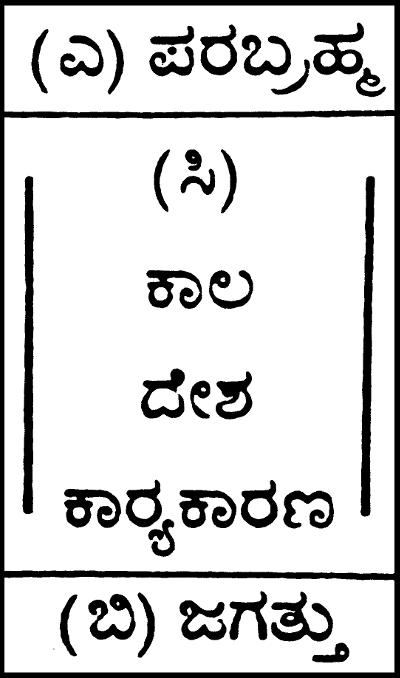
\includegraphics{images/001.jpg}
ಇಲ್ಲಿ (ಎ) ಎಂಬ ಪರಬ್ರಹ್ಮವಿದೆ. ಕೆಳಗೆ (ಬಿ) ಎಂಬ ಜಗತ್ತಿದೆ. ಪರಬ್ರಹ್ಮವು ಜಗತ್ತಾಗಿದೆ. ಜಗತ್ತು ಎಂದರೆ ಕೇವಲ ಜಡಜಗತ್ತು ಮಾತ್ರವಲ್ಲ; ಜೊತೆಗೆ ಮಾನಸಿಕ, ಆಧ್ಯಾತ್ಮಿಕ, –ಈ ವಿಶ್ವಗಳಲ್ಲಿ ಮತ್ತು ಸ್ವರ್ಗದಲ್ಲಿ ಏನಿವೆಯೊ ಅವೆಲ್ಲ. ಮನಸ್ಸು ಎಂಬುದು ಬದಲಾವಣೆಯ ಒಂದು ಹೆಸರು; ದೇಹ ಎಂಬುದು ಮತ್ತೊಂದು ಬದಲಾವಣೆಯ ಹೆಸರು. ಇಂಥ ಬದಲಾವಣೆಗಳೆಲ್ಲ ಸೇರಿ ವಿಶ್ವವಾಗಿದೆ. “ಎ” ಎಂಬ ಪರಬ್ರಹ್ಮ “ಸಿ” ಎಂಬ ಕಾಲ ದೇಶಗಳ–ಕಾರ್ಯ ಕಾರಣಗಳ ಮೂಲಕ ಪ್ರವೇಶಿಸಿ “ಬಿ” ಎಂಬ (ಎ) ಪರಬ್ರಹ್ಮ ಜಗತ್ತಾಗಿದೆ. ಇದೇ ಅದ್ವೈತದ ಮುಖ್ಯ ಭಾವನೆ. ಪರಬ್ರಹ್ಮನನ್ನು ನೋಡುವ ಗಾಜಿನಂತೆ ಇವೆ ಕಾಲ ದೇಶ ಕಾರ್ಯಕಾರಣ ಎಂಬುವು. ಅದನ್ನು ಕೆಳಗಿನ ದೃಷ್ಟಿಯಿಂದ ನೋಡಿದಾಗ ವಿಶ್ವದಂತೆ ತೋರುವುದು. ಆದ್ದರಿಂದ ಪರಬ್ರಹ್ಮನಲ್ಲಿ ಕಾಲ ದೇಶ ಕಾರಣಗಳಿಲ್ಲ ಎಂಬುದು ತಕ್ಷಣ ನಮಗೆ ಅರ್ಥವಾಗುತ್ತದೆ. ಮನಸ್ಸು, ಆಲೋಚನೆ ಅಲ್ಲಿ ಇಲ್ಲದುದರಿಂದ ಕಾಲದ ಭಾವನೆ ಅಲ್ಲಿ ಇರಲಾರದು. ಬಾಹ್ಯ ಬದಲಾವಣೆಗಳು ಅಲ್ಲಿ ಇಲ್ಲದೆ ಇರುವುದರಿಂದ ದೇಶದ ಭಾವನೆ ಅಲ್ಲಿ ಇರಲಾರದು. ಎಲ್ಲಿ ಒಂದು ಮಾತ್ರ ಇದೆಯೊ ಅಲ್ಲಿ ಚಲನೆ ಮತ್ತು ಕಾರಣ–ಇವು ಇರಲಾರವು. ನಾವು ಯಾವುದನ್ನು ಕಾರ್ಯಕಾರಣ ಸಂಬಂಧವೆನ್ನುವೆವೊ ಅದು ಪ್ರಾರಂಭವಾಗುವುದು, ಪರಬ್ರಹ್ಮವು ಇಂದ್ರಿಯ ಗೋಚರವಾಗುವಷ್ಟು ಅವನತಿಗೆ ಇಳಿದ ಮೇಲೆ, ಅದಕ್ಕೂ ಮೊದಲು ಅಲ್ಲ. ನಮ್ಮ ಇಚ್ಛೆ ಆಸೆ ಮುಂತಾದುವುಗಳೆಲ್ಲ ಅನಂತರ ಬರುವುವು. ಇದನ್ನು ನಾವು ಅರ್ಥಮಾಡಿಕೊಳ್ಳಬೇಕು; ಜ್ಞಾಪಕದಲ್ಲಿಡಬೇಕು. ಷೋಪನೇರನು ವೇದಾಂತ ತತ್ತ್ವವನ್ನು ವಿವರಿಸುವಾಗ ಒಂದು ತಪ್ಪು ಮಾಡಿರುವನೆಂದು ನನಗನ್ನಿಸುತ್ತದೆ. ಅದು ಇಚ್ಛೆಯನ್ನೇ ಸರ್ವಸ್ವವನ್ನಾಗಿ ಮಾಡಿರುವುದು. ಷೋಪನೇರ್​ ಪರ ಬ್ರಹ್ಮನ ಸ್ಥಾನದಲ್ಲಿ ಇಚ್ಛಾಶಕ್ತಿಯನ್ನು ನಿಲ್ಲಿಸುತ್ತಾನೆ. ಪರಬ್ರಹ್ಮನನ್ನು ಇಚ್ಛಾಶಕ್ತಿ ಎಂದು ಕರೆಯಲಾರೆವು. ಇಚ್ಛೆ ಬದಲಾಯಿಸುವಂತಹದು, ಇಂದ್ರಿಯ ಗೋಚರವಾದುದು. ದೇಶ, ಕಾಲ, ಕಾರ್ಯಕಾರಣಗಳು ಇವುಗಳ ಆಚೆ ಯಾವ ಬದಲಾವಣೆಯೂ ಇಲ್ಲ, ಯಾವ ಚಲನೆಯೂ ಇಲ್ಲ. ಅದರ ಆಚೆ ಮಾತ್ರ ಬಾಹ್ಯ ಚಲನೆ ಮತ್ತು ನಾವು ಆಲೋಚನೆ ಎಂದು ಕರೆಯುವ ಆಂತರಿಕ ಚಲನೆ ಪ್ರಾರಂಭವಾಗುವುದು. ಕಾಲ–ದೇಶ–ಕಾರ್ಯಕಾರಣಗಳಾಚೆ ಯಾವ ಇಚ್ಛಾಶಕ್ತಿಯೂ ಇರುವುದು ಸಾಧ್ಯವಿಲ್ಲ. ಆದಕಾರಣ ಇಚ್ಛೆ ಪ್ರಪಂಚಕ್ಕೆ ಹೇತುವಲ್ಲ. ನಾವಿನ್ನೂ ಸಮೀಪಕ್ಕೆ ಬಂದರೆ ನಮ್ಮ ದೇಹದಲ್ಲೆ ಆಗುವ ಪ್ರತಿಯೊಂದು ಬದಲಾವಣೆಗೂ ಇಚ್ಛೆಯೇ ಕಾರಣವಲ್ಲವೆಂಬುದು ತೇರುವುದು. ನಾನು ಕುರ್ಚಿಯನ್ನು ಚಲಿಸುತ್ತೇನೆ. ನನ್ನ ಇಚ್ಛೆಯೇ ಈ ಚಲನೆಗೆ ಕಾರಣ. ಈ ಇಚ್ಛಾಶಕ್ತಿ ಮಾಂಸಖಂಡದ ಚಲನೆಯಂತೆ ಮತ್ತೊಂದು ಕಡೆ ವ್ಯಕ್ತವಾಗುವುದು. ಕುರ್ಚಿಯನ್ನು ನೂಕುತ್ತಿರುವ ಶಕ್ತಿಯೇ, ಹೃದಯ ಶ್ವಾಸಕೋಶ ಇವುಗಳ ಚಲನೆಗೂ ಕಾರಣ. ಆದರೆ ಅದು ಪ್ರಜ್ಞಾಸ್ತರಕ್ಕೆ ಬಂದಾಗ ಮಾತ್ರ ಇಚ್ಛೆಯಾಗುವುದು. ಅದು ಈ ಸ್ಥಿತಿಗೆ ಬರುವುದಕ್ಕೆ ಮುಂಚೆ ಅದನ್ನು ಇಚ್ಛೆ ಎನ್ನುವುದು ತಪ್ಪು ಕಲ್ಪನೆಯಾಗುತ್ತದೆ. ಷೋಫನೇರನ ತತ್ತ್ವದಲ್ಲಿ ಇದರಿಂದಲೇ ಎಷ್ಟೋ ಗೊಂದಲವಾಗಿರುವುದು.

ಕಲ್ಲೊಂದು ಬೀಳುವುದು; ಏತಕ್ಕೆ ಎಂದು ನಾವು ಪ್ರಶ್ನಿಸುವೆವು. ಕಾರಣವಿಲ್ಲದೆ ಯಾವುದೂ ನಡೆಯದು ಎಂಬ ಊಹೆಯ ಆಧಾರದ ಮೇಲೆ ಈ ಪ್ರಶ್ನೆ ಸಾಧ್ಯ. ಮೊದಲು ಇದನ್ನು ಚೆನ್ನಾಗಿ ಗ್ರಹಿಸಿ ಎಂದು ಕೋರುತ್ತೇನೆ. ಯಾವಾಗಲಾದರೂ ಏತಕ್ಕೆ ಒಂದು ಘಟನೆ ಆಗುವುದು ಎಂದು ಪ್ರಶ್ನಿಸಿದಾಗ, ಪ್ರತಿಯೊಂದು ಘಟನೆಗೂ ಒಂದು ಕಾರಣವಿರಬೇಕು ಎಂದು ಊಹಿಸುವೆವು, ಎಂದರೆ ಇದಕ್ಕೆ ಮುಂಚೆ ಇದಕ್ಕೆ ಕಾರಣವಾದ ಯಾವುದೋ ಘಟನೆ ನಡೆದಿರಬೇಕು ಎಂದು ಅರ್ಥ. ಹಿಂದೆ ಆಗಿರುವುದನ್ನು ಮತ್ತು ಮುಂದೆ ಆಗುವುದನ್ನು ಕಾರ್ಯಕಾರಣ ಸಂಬಂಧ ಎನ್ನುವೆವು. ಎಂದರೆ ಪ್ರಪಂಚದಲ್ಲಿರುವ ಪ್ರತಿಯೊಂದೂ ಒಮ್ಮೆ ಕಾರಣವಾಗಿ ಅನಂತರ ಕಾರ್ಯವಾಗುವುದು. ಇದರ ಅನಂತರ ಬರುವುದಕ್ಕೆ ಇದೊಂದು ಕಾರಣವಾಗುವುದು. ಇದರ ಹಿಂದಿನದಕ್ಕೆ ಇದೇ ಒಂದು ಪರಿಣಾಮವಾಗುವುದು. ಇದೇ ಕಾರ್ಯಕಾರಣ ಸಂಬಂಧ. ನಮ್ಮ ಆಲೋಚನೆಗೆ ಇದು ಅತ್ಯಾವಶ್ಯಕ. ಪ್ರಪಂಚದಲ್ಲಿರುವ ಪ್ರತಿಯೊಂದು ಕಣವೂ, ಅದು ಏನಾದರೂ ಆಗಿರಲಿ, ಮತ್ತೊಂದು ಕಣದ ಸಂಬಂಧದ ದೃಷ್ಟಿಯಿಂದ ಮಾತ್ರ ಇದೆ ಎಂದು ನಂಬುತ್ತೇವೆ. ಈ ಭಾವನೆ ಹೇಗೆ ಬಂತು ಎಂದು ಬೇಕಾದಷ್ಟು ಚರ್ಚೆಯಾಗಿದೆ. ಯೂರೋಪಿನಲ್ಲಿ ಅಂತರ್​ದೃಷ್ಟಿಯುಳ್ಳ ತಾತ್ತ್ವಿಕರು ‘ಹಾಗೆ ನಂಬುವುದು ವ್ಯಕ್ತಿಯ ಸ್ವಭಾವದಲ್ಲೆ ಹುಟ್ಟಿಬಂದ ಗುಣ’ ಎನ್ನುವರು. ಮತ್ತೆ ಕೆಲವರು ಇದು ಅನುಭವದಿಂದ ಜನಿಸಿತು ಎನ್ನುವರು. ಈ ಪ್ರಶ್ನೆ ಇನ್ನೂ ಇತ್ಯರ್ಥವಾಗಿಲ್ಲ. ಈ ವಿಷಯದಲ್ಲಿ ವೇದಾಂತ ಏನು ಹೇಳುವುದೆಂಬುದನ್ನು ಮುಂದೆ ನೋಡೋಣ. ಆದರೆ ಮೊದಲು ನಾವು ಇದನ್ನು ತಿಳಿದುಕೊಳ್ಳಬೇಕು. ಅದೇನೆಂದರೆ ಏತಕ್ಕೆ ಎಂಬ ಪ್ರಶ್ನೆಯೇ ಸುತ್ತಲೂ ಇರುವ ಪ್ರತಿಯೊಂದು ವಸ್ತುಗಳ ಹಿಂದೆ ಏನು ಇದ್ದಿತು, ಅನಂತರ ಏನೊ ಇರುವುದು ಎಂಬ ಊಹೆಯ ಮೇಲೆ ನಿಂತಿದೆ ಎಂಬುದು. ಈ ಪ್ರಶ್ನೆಯಲ್ಲಿ ಸೇರಿರುವ ಮತ್ತೊಂದು ನಂಬಿಕೆ ಎಂದರೆ ಪ್ರಪಂಚದಲ್ಲಿ ಯಾವುದೂ ಸ್ವತಂತ್ರವಲ್ಲ, ಪ್ರತಿಯೊಂದೂ ಮತ್ತೊಂದು ವಸ್ತುವಿನ ಪ್ರಭಾವಕ್ಕೆ ಒಳಪಟ್ಟಿದೆ ಎಂಬುದು. ಅನ್ಯೋನ್ಯ ಆಶ್ರಯವೇ ವಿಶ್ವದ ನಿಯಮ. ಪರಬ್ರಹ್ಮವು ಯಾವುದರಿಂದಾಯಿತು ಎಂದು ಕೇಳುವುದರಿಂದ ಎಂತಹ ತಪ್ಪನ್ನು ಮಾಡುತ್ತಿರುವೆವು! ಈ ಪ್ರಶ್ನೆಯನ್ನು ಕೇಳಬೇಕಾದರೆ ಪರಬ್ರಹ್ಮ ಕೂಡ ಮತ್ತೊಂದರಿಂದ ಬದ್ಧವಾಗಿದೆ, ಮತ್ತೊಂದರ ಅಧೀನದಲ್ಲಿದೆ ಎಂದು ಊಹಿಸಬೇಕಾಗುತ್ತದೆ. ನಾವು ಹೀಗೆ ಊಹಿಸುವುದರಿಂದ ಬ್ರಹ್ಮವನ್ನು ಜಗತ್ತಿನ ಸ್ಥಿತಿಗೆ ಎಳೆಯುವೆವು. ನಿರಪೇಕ್ಷ ಸತ್ಯದಲ್ಲಿ ದೇಶಕಾಲ, ಕಾರ್ಯಕಾರಣ ಇವುಗಳಾವುವೂ ಇಲ್ಲ. ಏಕೆಂದರೆ ಅದು ಏಕವಾದುದು. ಯಾವುದು ಸ್ವತಃಸಿದ್ಧವಾಗಿರುವುದೊ ಅದಕ್ಕೆ ಮತ್ತಾವ ಕಾರಣವೂ ಬೇಕಾಗಿಲ್ಲ. ಸ್ವತಂತ್ರವಾದುದಕ್ಕೆ ಕಾರಣ ಮತ್ತಾವುದೂ ಇರಲಾರದು. ಇದ್ದರೆ ಅದು ಸ್ವತಂತ್ರವಾಗುತ್ತಿರಲಿಲ್ಲ; ಬದ್ಧವಾಗುತ್ತಿತ್ತು. ಸಾಪೇಕ್ಷವಾದುದು ಸ್ವತಂತ್ರವಾಗಲಾರದು. ನಿರಪೇಕ್ಷವಾದದ್ದು ಸಾಪೇಕ್ಷ ಹೇಗೆ ಆಯಿತು ಎಂದು ಕೇಳುವ ಪ್ರಶ್ನೆಯೇ ಅಸಹಜ; ಪರಸ್ಪರ ವಿರೋಧ. ಸೂಕ್ಷ್ಮದೃಷ್ಟಿಯನ್ನು ಬಿಟ್ಟು ವ್ಯಾವಹಾರಿಕವಾದ ಸಾಮಾನ್ಯ ಯುಕ್ತಿಯ ದೃಷ್ಟಿಯಿಂದ, ನಿರಪೇಕ್ಷವು ಸಾಪೇಕ್ಷ ಹೇಗೆ ಆಯಿತೆಂಬುದನ್ನು ನೋಡಬಹುದು. ಒಂದು ವೇಳೆ ಇದಕ್ಕೆ ಉತ್ತರ ಸಿಕ್ಕಿದರೆ ನಿರಪೇಕ್ಷವು ನಿರಪೇಕ್ಷವಾಗಿಯೆ ಉಳಿಯುವುದೆ? ಇಲ್ಲ, ಅದು ಸಾಪೇಕ್ಷವಾಗುವುದು. ನಮ್ಮ ಸಾಧಾರಣ ವ್ಯಾವಹಾರಿಕ ದೃಷ್ಟಿಯಿಂದ, ಜ್ಞಾನ ಎಂದರೇನು? ನಮ್ಮ ಮನಸ್ಸಿನ ಪರಿಮಿತಿಗೆ ಸಿಕ್ಕಿರುವ ಯಾವುದೊ ಒಂದು ವಸ್ತುವನ್ನು ನಾವು ತಿಳಿದಿರುವೆವು ಎನ್ನುವೆವು. ಅದು ನಮ್ಮ ಮನಸ್ಸನ್ನು ಮೀರಿಹೋಗಿದ್ದರೆ ಅದನ್ನು ನಾವು ತಿಳಿಯಲಾರೆವು. ಪರಬ್ರಹ್ಮವು ಮನಸ್ಸಿನ ಪರಿಮಿತಿಗೆ ಸಿಲುಕಿದರೆ ಅದು ಇನ್ನು ಪರಬ್ರಹ್ಮವಲ್ಲ, ಸಾಂತವಾಗುವುದು. ಮನಸ್ಸಿನ ಪರಿಮಿತಿಗೆ ಸಿಲುಕಿರುವುದೆಲ್ಲ ಸಾಂತವಾಗಿರುವುದು. ನಾನು ಪರಬ್ರಹ್ಮನನ್ನು ತಿಳಿಯುತ್ತೇನೆ ಎಂಬುದು ವಿರೋಧೋಕ್ತಿ. ಅದಕ್ಕೇ ಈ ಪ್ರಶ್ನೆಯನ್ನು ಬಗೆಹರಿಸುವುದು ಸಾಧ್ಯವಿಲ್ಲ. ಇದನ್ನು ಬಗೆಹರಿಸಲು ಸಾಧ್ಯವಾದರೆ ಅದು ಪರಬ್ರಹ್ಮವಾಗುವುದಿಲ್ಲ. ಜ್ಞಾತ ಬ್ರಹ್ಮನೇ ಅಲ್ಲ. ಅವನು ಕೂಡ ನಮ್ಮಂತೆ ಸಾಂತವಾಗಿರುವನು. ಅವನನ್ನು ತಿಳಿಯಲಾರೆವು. ಅವನು ಯಾವಾಗಲೂ ಅಜ್ಞಾತ.

ದೇವರೆಂಬುದು ಜ್ಞೇಯಕ್ಕಿಂತ ಮಿಗಿಲಾಗಿದೆ ಎಂದು ಅದ್ವೈತ ಹೇಳುವುದು. ಇದೊಂದು ತಿಳಿದುಕೊಳ್ಳಬೇಕಾದ ಮುಖ್ಯ ವಿಷಯ. ಆಜ್ಞೇಯತಾವಾದಿಗಳು ‘ನಾವು ದೇವರನ್ನು ತಿಳಿಯಲಾರೆವು’ ಎಂದು ಹೇಳುವ ದೃಷ್ಟಿಯಲ್ಲಿ ಇದನ್ನು ನೀವು ಅರ್ಥ ಮಾಡಿಕೊಳ್ಳಬಾರದು. ಉದಾಹರಣೆಗೆ ಇಲ್ಲೊಂದು ಕುರ್ಚಿ ಇದೆ. ಇದು ನಮಗೆ ಗೊತ್ತಿದೆ. ಆದರೆ ಆಕಾಶದ ಆಚೆ ಏನಿದೆ, ಅಲ್ಲಿ ಜನರಿರುವರೆ ಇಲ್ಲವೆ ಎಂಬುದನ್ನು ತಿಳಿಯುವುದು ಬಹುಶಃ ಅಸಾಧ್ಯ. ಈ ದೃಷ್ಟಿಯಲ್ಲಿ ದೇವರು ತಿಳಿದವನೂ ಅಲ್ಲ, ತಿಳಿಯದವನೂ ಅಲ್ಲ. ತಿಳಿದಿರುವುದಕ್ಕಿಂತ ಅವನು ಮಿಗಿಲು. ದೇವರು ನಮಗೆ ಗೊತ್ತಿಲ್ಲ, ಗೊತ್ತಾಗಲು ಸಾಧ್ಯವಿಲ್ಲ ಎಂಬುದರ ಅರ್ಥವೇ ಇದು. ಕೆಲವು ಪ್ರಶ್ನೆಗಳು ನಮಗೆ ಗೊತ್ತಿಲ್ಲ, ಗೊತ್ತಾಗಲು ಸಾಧ್ಯವಿಲ್ಲ ಎಂಬ ದೃಷ್ಟಿಯಿಂದ ಹೀಗೆ ಹೇಳಿಲ್ಲ. ದೇವರು ತಿಳಿದಿರುವುದಕ್ಕಿಂತ ಹೆಚ್ಚು. ಈ ಕುರ್ಚಿ ಗೊತ್ತಿದೆ. ಆದರೆ ದೇವರು ಇದಕ್ಕಿಂತಲೂ ಹೆಚ್ಚಾಗಿ ಗೊತ್ತಿರುವನು. ಏಕೆಂದರೆ ನಾವು ಅವನಿಂದ ಮಾತ್ರ, ಅವನ ಮೂಲಕ ಮಾತ್ರ ಕುರ್ಚಿಯನ್ನು ತಿಳಿದುಕೊಳ್ಳಬಹುದು. ಅವನು ಸಾಕ್ಷಿ, ಎಲ್ಲ ಜ್ಞಾನಕ್ಕೂ ನಿತ್ಯಸಾಕ್ಷಿ. ನಮಗೆ ಗೊತ್ತಿರುವುದೆಲ್ಲ ಅವನಿಂದ ಮಾತ್ರ, ಅವನ ಮೂಲಕ ಮಾತ್ರ. ಅವನೇ ನಮ್ಮ ಆತ್ಮದ ಸಾರ. ಅವನೇ ನಮ್ಮ ಅಹಂಕಾರದ ಮೂಲ. ನಾವು ಏನನ್ನು ಬೇಕಾದರೂ ಈ ಅಹಂಕಾರದ ಮೂಲಕ ಮಾತ್ರ ತಿಳಿಯಲು ಸಾಧ್ಯ. ಆದಕಾರಣವೇ ಪ್ರತಿಯೊಂದೂ ಬ್ರಹ್ಮನ ಮೂಲಕ ಮಾತ್ರ ಸಾಧ್ಯ. ಕುರ್ಚಿಯನ್ನು ತಿಳಿಯಬೇಕಾದರೆ ದೇವರಲ್ಲಿ ಮಾತ್ರ ದೇವರ ಮೂಲಕ ಮಾತ್ರ ಸಾಧ್ಯ. ಆದಕಾರಣವೆ ದೇವರು ಕುರ್ಚಿಗಿಂತಲೂ ಹೆಚ್ಚು ಸಮೀಪದಲ್ಲಿರುವನು. ಆದರೂ ಅದಕ್ಕಿಂತಲೂ ಅತ್ಯಂತ ಮೇಲಾಗಿರುವನು. ದೇವರೆಂಬುವನು ತಿಳಿದಿರುವುದೂ ಅಲ್ಲ, ತಿಳಿಯದುದೂ ಅಲ್ಲ. ಇವೆರಡಕ್ಕೂ ಅನಂತವಾಗಿ ಮೀರಿರುವನು. ಅವನೇ ಆತ್ಮ. “ಆ ಪುಣ್ಯಾತ್ಮ ವ್ಯಾಪಿಸದೇ ಇದ್ದರೆ ಈ ಪ್ರಪಂಚದಲ್ಲಿ ಯಾರು ಒಂದು ಕ್ಷಣವಾದರೂ ಬದುಕುತ್ತಿದ್ದರು, ಉಸಿರಾಡುತ್ತಿದ್ದರು?” ಅವನಿಂದ ಮಾತ್ರ, ಅವನ ಮೂಲಕ ಮಾತ್ರ ಉಸಿರಾಡುವೆವು, ಅವನಿಂದ ಮಾತ್ರ, ಅವನ ಮೂಲಕ ಮಾತ್ರ ಜೀವಿಸಿರುವೆವು. ಅವನೆಲ್ಲೊ ನಿಂತು ನನ್ನ ರಕ್ತವು ಚಲಿಸುವಂತೆ ಮಾಡುತ್ತಿರುವನು ಎಂದೇನೂ ಅಲ್ಲ. ಅವನೇ ಇವುಗಳೆಲ್ಲದರ ಸಾರ, ಆತ್ಮದ ಆತ್ಮ. ಅವನು ನಮಗೆ ಗೊತ್ತಿರುವನೆಂದು ಯಾವ ವಿಧದಲ್ಲಿಯೂ ಹೇಳಲಾರೆವು; ಹೇಳಿದರೆ ಅವನನ್ನು ಅಧೋಗತಿಗೆ ಒಯ್ದಂತೆ. ನೀವು ನಿಮ್ಮನ್ನು ಮೀರಿ ಹೋಗಲಾರಿರಿ. ಅದಕ್ಕೇ ನೀವು ಅವನನ್ನು ತಿಳಿಯಲಾರಿರಿ. ವಿಷಯೀಕರಣವೇ ಜ್ಞಾನ. ಉದಾಹರಣೆಗೆ, ನಿಮ್ಮ ನೆನಪಿನಲ್ಲಿ ಹಲವು ವಸ್ತುಗಳನ್ನು ಮೂರ್ತೀಕರಿಸುತ್ತಿರುವಿರಿ. ಅವನ್ನು ನಿಮ್ಮಿಂದ ಹೊರಗೆ ಆರೋಪ ಮಾಡುತ್ತಿರುವಿರಿ. ನನ್ನ ನೆನಪು ಎಂದರೆ ನಾನು ನೋಡಿದ ಮತ್ತು ತಿಳಿದ ವಿಷಯಗಳೆಲ್ಲ ನನ್ನ ಮನಸ್ಸಿನಲ್ಲಿರುವುವು ಎಂದು. ಅದನ್ನು ನಾನು ತಿಳಿಯಲು ಪ್ರಯತ್ನಪಟ್ಟಾಗ, ಆಲೋಚಿಸಲು ಪ್ರಯತ್ನಪಟ್ಟಾಗ, ಮಾಡುವ ಪ್ರಥಮ ಕ್ರಿಯೆಯೇ ಅದನ್ನು ಹೊರಗೆ ಆರೋಪಿಸುವುದು. ನಾವು ಬ್ರಹ್ಮನನ್ನು ಈ ದೃಷ್ಟಿಯಿಂದ ನೋಡಲು ಸಾಧ್ಯವಿಲ್ಲ. ಏಕೆಂದರೆ ಅವನೇ ನಮ್ಮ ಆತ್ಮದ ಸಾರ. ನಮ್ಮಿಂದ ಹೊರಗೆ ಅವನನ್ನು ಆರೋಪಿಸಲು ಸಾಧ್ಯವೇ ಇಲ್ಲ. ವೇದಾಂತದಲ್ಲೆಲ್ಲಾ ಅತಿಗಹನವಾದ ಭಾವನೆಯೇ ಇದು. “ಓ ಶ್ವೇತಕೇತು, ಯಾವನು ನಿನ್ನ ಜೀವದ ಸಾರವೊ ಅವನೇ ಸತ್ಯ, ಅವನೇ ಆತ್ಮ, ನೀನೆ ಅವನು, ನೀನೆ ಬ್ರಹ್ಮ” “ನೀನೇ ದೇವರು” ಎಂಬುದರ ಅರ್ಥ ಇದೇ. ಅವನನ್ನು ನೀವು ಮತ್ತಾವ ಭಾಷೆಯ ಮೂಲಕವೂ ವ್ಯಕ್ತಗೊಳಿಸಲಾರಿರಿ. ಅವನನ್ನು ನಮ್ಮ ತಂದೆ, ಸಹೋದರ, ಪ್ರೀತಿ ಪಾತ್ರ ಸಖ ಎಂದು ಕರೆಯುವ ಭಾಷೆಯ ಪ್ರಯತ್ನವೆಲ್ಲ ಅವನನ್ನು ಇಂದ್ರಿಯ ಗೋಚರನನ್ನಾಗಿ ಮಾಡುವ ಯತ್ನ. ನಾವು ಹಾಗೆ ಮಾಡಲಾರೆವು. ಅವನೇ ಎಲ್ಲಕ್ಕೂ ನಿತ್ಯಸಾಕ್ಷಿ. ನಾನು ಈ ಮೇಚಿನ ಜ್ಞಾತೃ, ನಾನು ಮೇಜನ್ನು ನೋಡುತ್ತೇನೆ. ಹಾಗೆಯೇ ಬ್ರಹ್ಮ ನನ್ನಾತ್ಮಾದ ನಿತ್ಯ ಜ್ಞಾತೃ. ನಿಮ್ಮ ಆತ್ಮದ ಸಾರವನ್ನೇ, ಸರ್ವದ ಸತ್ಯವನ್ನೇ ನೀವು ಹೇಗೆ ವಿಷಯೀಕರಿಸುವಿರಿ? ನಾನು ಮತ್ತೊಮ್ಮೆ ನಿಮಗೆ ಹೇಳುತ್ತೇನೆ–\break ಬ್ರಹ್ಮವನ್ನು ಜ್ಞೇಯವೆಂದು ಅಥವಾ ಅಜ್ಞೇಯವೆಂದು ಹೇಳಲಾಗುವುದಿಲ್ಲ. ಅವನು ಇವೆರಡನ್ನೂ ಅನಂತವಾಗಿ ಮೀರಿರುವನು. ಅವನು ನಮ್ಮೊಂದಿಗೆ ಒಂದಾಗಿರುವನು. ಯಾವುದು ಒಂದಾಗಿರುವುದೋ ಅದು ನಮ್ಮ ಆತ್ಮನಂತೆಯೇ ಜ್ಞೇಯವೂ ಅಲ್ಲ, ಅಜ್ಞೇಯವೂ ಅಲ್ಲ. ನೀವು ನಿಮ್ಮ ಆತ್ಮನನ್ನೇ ತಿಳಿಯಲಾರಿರಿ. ಅದನ್ನು ನೀವು ಹೊರಕ್ಕೆ ತಂದು ನೋಡಬೇಕಾದ ವಸ್ತುವನ್ನಾಗಿ ಮಾಡಲಾರಿರಿ. ಏಕೆಂದರೆ ನೀವೇ ಅದಾಗಿರುವಿರಿ. ನೀವು ಅದರಿಂದ ಬೇರೆ ಆಗಲಾರಿರಿ. ಅದು ಅಜ್ಞೇಯವೂ ಅಲ್ಲ. ನಿಮ್ಮ ಆತ್ಮನಿಗಿಂತ ಯಾವುದು ತಾನೇ ನಿಮಗೆ ಚೆನ್ನಾಗಿ ಗೊತ್ತಿದೆ? ಇದೇ ನಮ್ಮ ಜ್ಞಾನದ ಕೇಂದ್ರ. ಇದೇ ರೀತಿ ಬ್ರಹ್ಮವು ಜ್ಞೇಯವೂ ಅಲ್ಲ, ಅಜ್ಞೇಯವೂ ಅಲ್ಲ, ಆದರೆ ಅವರೆಡನ್ನೂ ಮೀರಿದುದು. ಏಕೆಂದರೆ ಬ್ರಹ್ಮವೇ ನಿಜವಾದ ನಮ್ಮ ಆತ್ಮ.

ಬ್ರಹ್ಮನಿಗೆ ಯಾವುದು ಕಾರಣ ಎಂಬ ಪ್ರಶ್ನೆಯೇ ಮೊದಲು ಅಸಮಂಜಸ, ಎರಡನೆಯದಾಗಿ ಅದ್ವೈತದಲ್ಲಿ ಬರುವ ಬ್ರಹ್ಮಭಾವನೆ ಏಕತೆ. ಆದಕಾರಣ ಅವನನ್ನು ನಾವು ವಿಷಯೀಕರಿಸಲಾರೆವು. ನಮಗೆ ಗೊತ್ತಿರಲಿ, ಇಲ್ಲದೆ ಇರಲಿ, ನಾವು ಯಾವಾಗಲೂ ಅವನಲ್ಲಿ ಜೀವಿಸಿ ಸಂಚರಿಸುತ್ತಿರುವೆವು. ನಾವು ಏನನ್ನು ಮಾಡಿದರೂ ಅದು ಯಾವಾಗಲೂ ಅವನಿಂದ. ದೇಶ ಕಾಲ ಕಾರ್ಯಕಾರಣ–ಇವುಗಳೆಂದರೇನು ಎಂಬುದೇ ಈಗಿನ ಪ್ರಶ್ನೆ. ಅದ್ವೈತವೆಂದರೆ ದ್ವೈತವಲ್ಲದುದು; ಎರಡಲ್ಲ ಒಂದೇ ಎಂಬುದು. ದೇಶಕಾಲ–ಕಾರ್ಯ ಕಾರಣಗಳ ಮೂಲಕ ಏಕವು ಅನೇಕವಾಗಿದೆ ಎಂಬ ಪ್ರಮೇಯವಿದೆ. ಬ್ರಹ್ಮ ಮತ್ತು ಮಾಯೆ (ದೇಶಕಾಲ–ಕಾರ್ಯ ಕಾರಣಗಳ ಮೊತ್ತ) ಎರಡೂ ಇರುವಂತೆ ತೋರುತ್ತಿದೆ. ಎರಡೂ ಇವೆ ಎಂದು ಸದ್ಯಕ್ಕೆ  ಒಪ್ಪುವಂತೆಯೇ ತೋರುತ್ತದೆ. ಅದ್ವೈತಿ ಅದನ್ನು ಎರಡು ಎಂದು ಹೇಳಲಾಗುವುದಿಲ್ಲ, ಎನ್ನುತ್ತಾನೆ. ಎರಡು ಇರಬೇಕಾದರೆ ಕಾರಣರಹಿತವಾದ ಎರಡು ಪ್ರತ್ಯೇಕ ನಿರಪೇಕ್ಷವಸ್ತುಗಳು ಇರಬೇಕಾಗುವುದು. ಮೊದಲನೆಯದಾಗಿ ಕಾಲದೇಶ ಕಾರ್ಯಕಾರಣ ಇವು ಸ್ವತಂತ್ರವೆನ್ನಲಾಗುವುದಿಲ್ಲ. ಕಾಲವು ಮತ್ತೊಂದನ್ನು ಆಶ್ರಯಿಸಬೇಕು. ನಮ್ಮ ಮನಸ್ಸು ಬದಲಾವಣೆಯನ್ನು ಹೊಂದಿದಂತೆ ಅದೂ ಬದಲಾಗುವುದು. ಕೆಲವು ವೇಳೆ ಸ್ವಪ್ನದಲ್ಲಿ ಹಲವು ವರುಷಗಳವರೆಗೆ ಬಾಳಿದಂತೆ ತೋರುತ್ತದೆ. ಮತ್ತೆ ಕೆಲವು ವೇಳೆ ಹಲವು ತಿಂಗಳುಗಳು ಒಂದು ಕ್ಷಣದಂತೆ ಕಳೆದುಹೋದವು ಎಂಬಂತೆ ಭಾಸವಾಗುತ್ತದೆ. ಆದುದರಿಂದ ಕಾಲವು ಸಂಪೂರ್ಣವಾಗಿ ನಮ್ಮ ಮನಸ್ಸನ್ನು ಆಶ್ರಯಿಸಿಕೊಂಡಿದೆ. ಎರಡನೆಯದಾಗಿ ಕೆಲವು ವೇಳೆ ಕಾಲದ ಭಾವನೆ ಸಂಪೂರ್ಣ ಮಾಯವಾಗುವುದು. ಇದರಂತೆಯೇ ದೇಶವೂ ಕೂಡ. ದೇಶವೆಂದರೇನೆಂಬುದು ನಮಗೆ ಗೊತ್ತಾಗುವುದಿಲ್ಲ. ಆದರೂ ಅದು ಇದೆ. ಅದನ್ನು ವಿವರಿಸಲಾಗುವುದಿಲ್ಲ. ಮತ್ತೊಂದರ ಆಶ್ರಯವಿಲ್ಲದೆ ಇದು ಇರಲಾರದು. ಇದರಂತೆಯೇ ಕಾರ್ಯಕಾರಣವೂ.

ಕಾಲ ದೇಶ ಕಾರ್ಯ ಕಾರಣ ಇವುಗಳ ವಿಶಿಷ್ಟ ಸ್ವಭಾವವೆಂದರೆ ಅವು ಮತ್ತೊಂದರ ಆಶ್ರಯವಿಲ್ಲದೆ ಇರಲಾರವು. ಬಣ್ಣ ಮೇರೆ ಇವುಗಳ ಮತ್ತು ಮತ್ತೊಂದರ ಸಂಬಂಧವಿಲ್ಲದ ಕೇವಲ ಆಕಾಶವನ್ನು (ದೇಶವನ್ನು) ಕುರಿತು ಯೋಚಿಸಲೆತ್ನಿಸಿ. ಅದು ಸಾಧ್ಯವೇ ಇಲ್ಲ.\break ದೇಶವನ್ನು ಎರಡು ಮೇರೆಗಳ ಮಧ್ಯದಲ್ಲಿರುವುದು ಅಥವಾ ಮೂರು ವಸ್ತುಗಳ ಮಧ್ಯದಲ್ಲಿರುವುದು ಎಂದು ಭಾವಿಸಬೇಕಾಗುವುದು. ಅದು ಇರಬೇಕಾದರೆ ಯಾವುದಾದರೊಂದು ವಸ್ತುವಿನ ಸಂಬಂಧವಿರಬೇಕು. ಇದರಂತೆಯೇ ಕಾಲವೂ ಕೂಡ. ಕೇವಲ ಸ್ವತಂತ್ರವಾದ ಕಾಲದ ಭಾವನೆ ನಮಗೆ ಸಾಧ್ಯವೇ ಇಲ್ಲ. ಹಿಂದೆ ಆದುದು, ಮುಂದೆ ಆಗುವುದು, ಎಂಬ ಎರಡು ಘಟನೆಗಳನ್ನು ತೆಗೆದುಕೊಂಡು ಅವನ್ನು ಅನುಕ್ರಮದಲ್ಲಿ ಜೋಡಿಸಬೇಕು. ದೇಶವನ್ನೂ ನಾವು ಹೇಗೆ ಹೊರಗೆ ಇರುವ ವಸ್ತುವಿನೊಂದಿಗೆ ಸಂಬಂಧಿಸಬೇಕೊ ಹಾಗೆಯೆ ಕಾಲಕ್ಕೂ ಎರಡು ಘಟನೆಗಳ ಆಶ್ರಯಬೇಕು. ಕಾರ್ಯಕಾರಣಗಳ ಭಾವನೆಯನ್ನು ಕಾಲದೇಶಗಳಿಂದ ಬೇರ್ಪಡಿಸಲಾಗುವುದೇ ಇಲ್ಲ. ಇದೇ ಅವುಗಳ ವಿಶಿಷ್ಟ ಸ್ವಭಾವ. ಅವಕ್ಕೆ ಸ್ವತಂತ್ರ ಅಸ್ತಿತ್ವವಿಲ್ಲ. ಕುರ್ಚಿ ಗೋಡೆಗಳಿಗೆ ಇರುವ ಅಸ್ತಿತ್ವ ಕೂಡ ಅವಕ್ಕೆ ಇಲ್ಲ. ಅವು ಎಲ್ಲ ವಸ್ತುಗಳ ಹಿಂದೆ ಇರುವ ಛಾಯೆಯಂತೆ ಇವೆ. ನೀವು ಅವನ್ನು ಹಿಡಿಯಲಾರಿರಿ. ಅವಕ್ಕೇ ಸ್ವತಂತ್ರ ಅಸ್ತಿತ್ವವಿಲ್ಲ. ಆದರೂ ಅವು ಇಲ್ಲವೆಂದಲ್ಲ, ಏಕೆಂದರೆ ಅವುಗಳ ಮೂಲಕ ಮಾತ್ರ ವಿಶ್ವವು ವ್ಯಕ್ತವಾಗುತ್ತಿದೆ. ಮೊದಲನೆಯದಾಗಿ ಕಾಲದೇಶ ಕಾರ್ಯಕಾರಣಗಳ ಸಂಯೋಗ ಇದೆ ಅಥವಾ ಇಲ್ಲ ಎಂದು ಹೇಳಲಾರೆವು. ಎರಡನೆಯದಾಗಿ ಕೆಲವು ವೇಳೆ ಅದು ಅದೃಶ್ಯವಾಗುವುದು. ಉದಾಹರಣೆಗೆ, ಸಮುದ್ರದಲ್ಲಿ ಒಂದು ಅಲೆ ಇದೆ ಎಂದು ಭಾವಿಸೋಣ. ನಿಜವಾಗಿ ಅಲೆಯೂ ಸಮುದ್ರವೇ ಆದರೂ ಅಲೆ ಸಮುದ್ರದಿಂದ ಬೇರೆ ಎಂದು ಭಾವಿಸುತ್ತೇವೆ. ಈ ವ್ಯತ್ಯಾಸಕ್ಕೆ ಕಾರಣವೇನು? ನಾಮರೂಪ, ಎಂದರೆ ಮನಸ್ಸಿನಲ್ಲಿ ಇರುವ ಅದರ ಭಾವನೆ ಮತ್ತು ರೂಪ. ಅಲೆ ಸಮುದ್ರದಿಂದ ಬೇರೆ ಎಂದು ಯೋಚಿಸಲು ಸಾಧ್ಯವೆ? ಎಂದಿಗೂ ಇಲ್ಲ. ಯಾವಾಗಲೂ ಅದಕ್ಕೆ ಸಮುದ್ರದ ಭಾವನೆಯೊಂದಿಗೆ ಸಂಬಂಧವಿದೆ. ಅಲೆ ನಿಂತರೆ ತಕ್ಷಣ ಅದರ ರೂಪ ಮಾಯವಾಗುವುದು. ಆದರೂ ಇದು ಒಂದು ಭ್ರಾಂತಿಯಲ್ಲ. ಎಲ್ಲಿಯವರೆಗೂ ಅಲೆ ಇತ್ತೊ ಅಲ್ಲಿಯವರೆಗೆ ರೂಪ ಇತ್ತು. ನಾವು ಅದನ್ನು ನೋಡಲೇಬೇಕಾಗಿತ್ತು; ಇದೇ ಮಾಯೆ.

ಆದುದರಿಂದ, ಈ ವಿಶ್ವವೆಲ್ಲ ಒಂದು ವಿಚಿತ್ರ ರೀತಿಯಲ್ಲಿದೆ. ಪರಬ್ರಹ್ಮವೇ ಒಂದು ಸಾಗರ. ನಾವು, ನೀವು, ಸೂರ್ಯ, ನಕ್ಷತ್ರ ಮುಂತಾದುವುಗಳೆಲ್ಲ ಆ ಸಾಗರದ ಅಲೆಗಳು. ಅಲೆಯನ್ನು ಬೇರ್ಪಡಿಸುವುದಾವುದು? ರೂಪವೊಂದೇ. ಅದೇ ಕಾಲ, ದೇಶ ಕಾರ್ಯಕಾರಣ. ಎಲ್ಲ ಅಲೆಯ ಆಧಾರದ ಮೇಲಿದೆ. ಅಲೆ ನಿಂತೊಡನೆ ಕಾಲ, ದೇಶ, ಕಾರ್ಯಕಾರಣಗಳೂ ಮಾಯವಾಗುತ್ತವೆ. ವ್ಯಕ್ತಿಯೆ ಮಾಯೆಯನ್ನು ತ್ಯಜಿಸಿದರೆ ಅವನು ಮುಕ್ತನಾಗುವನು. ತನ್ನ ಮಾರ್ಗದಲ್ಲಿ ಯಾವಾಗಲೂ ಕಂಟಕಪ್ರಾಯವಾಗಿರುವ ಕಾಲ ದೇಶ ಮತ್ತು ಕಾರ್ಯಕಾರಣ ಇವುಗಳ ಮೇಲಿರುವ ಆಸಕ್ತಿಯನ್ನು ತ್ಯಜಿಸುವುದಕ್ಕೆ ಮಾನವ ಹೋರಾಡುವನು. ವಿಕಾಸವಾದವೆಂದರೇನು? ಎರಡು ಮುಖ್ಯ ವಿಷಯಗಳು ಯಾವುವು? ಸುಪ್ತವಾಗಿರುವ ಅದ್ಭುತ ಶಕ್ತಿ ವ್ಯಕ್ತವಾಗಲು ಯತ್ನಿಸುತ್ತಿದೆ. ಪರಿಸ್ಥಿತಿ ಅದಕ್ಕೆ ಆತಂಕವನ್ನು ಉಂಟುಮಾಡುತ್ತದೆ; ವ್ಯಕ್ತಗೊಳ್ಳುವುದಕ್ಕೆ ಅವಕಾಶ ಕೊಡುತ್ತಿಲ್ಲ. ಪರಿಸ್ಥಿತಿಯೊಂದಿಗೆ ಹೋರಾಡಲು ಅದು ಹೊಸ ಹೊಸ ದೇಹಗಳನ್ನು ಧರಿಸುತ್ತದೆ. ಈ ಹೋರಾಟದಲ್ಲಿ ಜೀವಾಣು ಮತ್ತೊಂದು ದೇಹವನ್ನು ಪಡೆದು ಹಲವು ಆತಂಕಗಳಿಂದ ಪಾರಾಗುವುದು. ಹೀಗೆ ಮನುಷ್ಯನ ಜನ್ಮವನ್ನು ಪಡೆಯುವವರೆಗೂ ಬೇರೆ ಬೇರೆ ದೇಹಗಳನ್ನು ಪಡೆಯುತ್ತ ಹೋಗುವುದು. ತಾರ್ಕಿಕರೀತಿಯಲ್ಲಿ ಈ ಭಾವನೆಯ ಪರಾಕಾಷ್ಠೆಗೆ ನಾವು ಬಂದರೆ, ಯಾವ ಶಕ್ತಿ ಜೀವಾಣುವಿನಲ್ಲಿತ್ತೋ, ಯಾವುದು ಅದನ್ನು ಮಾನವನಂತೆ ಮಾಡಿತೋ ಅದೇ ಶಕ್ತಿ ಪ್ರಕೃತಿಯೊಡ್ಡುವ ಆತಂಕಗಳೆಲ್ಲದರಿಂದ ಪಾರಾಗಿ, ಪರಿಸ್ಥಿತಿಯಿಂದ ಮುಕ್ತವಾಗುವ ಒಂದು ಸಮಯಕ್ಕೂ ಬರಲೇಬೇಕಾಗುವುದು. ಇದನ್ನು ತಾತ್ತ್ವಿಕ ರೀತಿಯಲ್ಲಿ ವಿವರಿಸುವುದಾದರೆ, ಅದು ಈ ರೂಪವನ್ನು ಧಾರಣ ಮಾಡುವುದು: ಪ್ರತಿಯೊಂದು ಘಟನೆಗೂ ಎರಡು ಭಾಗಗಳಿವೆ. ಒಂದು ವಿಷಯಿ, ಮತ್ತೊಂದು ವಿಷಯ. ವಿಷಯಿಯು ವಿಷಯದ (ಬಾಹ್ಯವಸ್ತುವಿನ) ಸ್ವಾಮಿಯಾಗಬೇಕೆಂಬುದು ಜೀವನದ ಒಂದು ಗುರಿ. ಉದಾಹರಣೆಗೆ, ಒಬ್ಬ ನನ್ನನ್ನು ನಿಂದಿಸುತ್ತಾನೆ. ಅದರಿಂದ ನಾನು ದುಃಖಿಯಾಗುತ್ತೇನೆ. ಪರಿಸ್ಥಿತಿಯನ್ನು ಇದಿರಿಸುವಷ್ಟು ಸಮರ್ಥನಾಗುವುದೆ ನನ್ನ ಹೋರಾಟದ ಗುರಿಯಾಗುವುದು. ಅವನು ನನ್ನನ್ನು ನಿಂದಿಸಿದರೂ ನನ್ನ ಮೇಲೆ ಪರಿಣಾಮವಾಗಕೂಡದು. ನಾವೆಲ್ಲ ಇದರಿಂದ ಪಾರಾಗುವುದಕ್ಕೆ ಯತ್ನಿಸುತ್ತಿರುವುದೇ ಹೀಗೆ. ನೀತಿ ಎಂದರೇನು? ವಿಷಯಿಯನ್ನು ಪರಬ್ರಹ್ಮನೊಂದಿಗೆ ಸಮಶ್ರುತಿಗೊಳಿಸಿ ಅವನನ್ನು ಬಲಗೊಳಿಸುವುದೇ ನೀತಿ. ಇದರಿಂದ ಬಾಹ್ಯ ಪ್ರಕೃತಿಗೆ ನಮ್ಮ ಮೇಲೆ ಯಾವ ಸ್ವಾಧೀನತೆಯೂ ಇರುವುದಿಲ್ಲ. ಎಲ್ಲ ಸನ್ನಿವೇಶಗಳನ್ನೂ ಜಯಿಸುವ ಒಂದು ಸಮಯ ಬಂದೇ ಬರುವುದೆಂಬುದು ನಮ್ಮ ವೇದಾಂತದ ಸಿದ್ಧಾಂತ, ಏಕೆಂದರೆ, ಪ್ರಕೃತಿಯು ಸಾಂತವಾದದ್ದು.

ನಾವು ಇಲ್ಲಿ ಮತ್ತೊಂದು ವಿಷಯವನ್ನು ಕಲಿಯಬೇಕಾಗಿದೆ. ಪ್ರಕೃತಿ ಸಾಂತವೆಂದು ನಮಗೆ ಹೇಗೆ ಗೊತ್ತು? ಇದನ್ನು ನಾವು ಕೇವಲ ತತ್ತ್ವಶಾಸ್ತ್ರದಿಂದ ಮಾತ್ರ ತಿಳಿಯಬಹುದು. ಸಾಂತವಾಗಿರುವ ಆ ಅನಂತವೇ ಪ್ರಕೃತಿ. ಆದಕಾರಣ ಇದು ಸಾಂತ. ಪರಿಸ್ಥಿತಿಯನ್ನೆಲ್ಲ ಗೆಲ್ಲುವ ಒಂದು ಕಾಲ ಬಂದೇ ಬರುವುದು. ನಾವು ಅದನ್ನು ಗೆಲ್ಲುವುದು ಹೇಗೆ? ಎಲ್ಲ ವಾಸ್ತವಿಕ ಪರಿಸ್ಥಿತಿಗಳನ್ನೂ ನಾವು ಗೆಲ್ಲದೆ ಇರಬಹುದು; ಅದು ಸಾಧ್ಯವೇ ಇಲ್ಲ. ಕಿರುಮೀನೊಂದು ನೀರಿನಲ್ಲಿ ತನ್ನ ವೈರಿಗಳಿಂದ ಪಾರಾಗಲು ಯತ್ನಿಸುವುದು. ಅದನ್ನು ಹೇಗೆ ಮಾಡುವುದು? ರೆಕ್ಕೆಗಳನ್ನು ಬೆಳಸಿಕೊಂಡು ಒಂದು ಹಕ್ಕಿಯಾಗುವುದರಿಂದ. ನೀರನ್ನು ಅಥವಾ ಗಾಳಿಯನ್ನು ಮೀನು ಬದಲಾಯಿಸಲಿಲ್ಲ. ಬದಲಾವಣೆ ಅದರಲ್ಲಿಯೇ ಆಯಿತು. ಬದಲಾವಣೆ ಯಾವಾಗಲೂ ವ್ಯಕ್ತಿಗತವಾದುದು. ಪ್ರಕೃತಿಯ ಮೇಲೆ ಆಗುವ ಗೆಲುವು ವ್ಯಕ್ತಿಯಲ್ಲಿ ಆದ ಬದಲಾವಣೆಯಿಂದ ಉಂಟಾಗುವುದು ಎಂಬುದು ವಿಕಾಸದಲ್ಲೆಲ್ಲಾ ನಿಮಗೆ ಕಾಣುವುದು. ಇದನ್ನು ಧರ್ಮಕ್ಕೆ ಮತ್ತು ನೀತಿಗೆ ಅನ್ವಯಿಸಿದರೆ ಪಾಪವನ್ನು ಗೆಲ್ಲುವುದು ವ್ಯಕ್ತಿಯ ಬದಲಾವಣೆಯಿಂದ ಮಾತ್ರ ಸಾಧ್ಯ ಎಂಬುದು ಗೊತ್ತಾಗುತ್ತದೆ. ಆದಕಾರಣವೇ ಅದ್ವೈತ ವೇದಾಂತದಲ್ಲಿ ವ್ಯಕ್ತಿಗೆ ಇಷ್ಟೊಂದು ಪ್ರಾಧಾನ್ಯ. ಪಾಪ ಮತ್ತು ದುಃಖವನ್ನು ಕುರಿತು ಮಾತನಾಡುವುದರಲ್ಲಿ ಅರ್ಥವಿಲ್ಲ. ಏಕೆಂದರೆ ಅವು ಮನುಷ್ಯನಿಂದ ಹೊರಗೆ ಇಲ್ಲ. ನಾನು ಕೋಪಕ್ಕೆ ಒಗ್ಗಿಹೋದರೆ ಕೋಪಿಸಿಕೊಳ್ಳುವುದೇ ಇಲ್ಲ. ನಾನು ಯಾವ ದ್ವೇಷಕ್ಕೂ ಜಗ್ಗದವನಾದರೆ ನನ್ನಲ್ಲಿ ದ್ವೇಷವೇ ಇರುವುದಿಲ್ಲ.

ಆದುದರಿಂದ ವ್ಯಕ್ತಿಯ ಮೂಲಕ, ವ್ಯಕ್ತಿಯನ್ನು ಪೂರ್ಣಗೊಳಿಸುವ ಮೂಲಕ ಆ ದಿಗ್ವಿಜಯವನ್ನು ಸಂಪಾದಿಸಬಹುದು. ಭೌತಿಕ ಮತ್ತು ನೈತಿಕ ಮಾರ್ಗದಲ್ಲಿ ನವ ನವಾನ್ವೇಷಣೆಗಳನ್ನು ಒಪ್ಪಿಕೊಂಡು, ಕೆಲವು ವೇಳೆ ಅವನ್ನೂ ಮೀರಿಹೋಗಬಲ್ಲ ಕೆಚ್ಚು ಅದ್ವೈತ ವೇದಾಂತ ಒಂದಕ್ಕೇ ಇರುವುದು ಎಂದು ನಾನು ಧೈರ್ಯವಾಗಿ ಹೇಳುತ್ತೇನೆ. ಆಧುನಿಕ ವೈಜ್ಞಾನಿಕರಿಗೆ ಇದರ ಮೇಲೆ ಅಷ್ಟು ಒಲವು ಮೂಡುವುದಕ್ಕೂ ಇದೇ ಕಾರಣ. ಪುರಾತನ ದ್ವೈತಸಿದ್ಧಾಂತಗಳು ಅವರಿಗೆ ಸಾಲವು, ಅವರ ಆವಶ್ಯಕತೆಯನ್ನು ಅವು ಪೂರ್ಣಮಾಡಲಾರವು. ಮನುಷ್ಯನಿಗೆ ಶ್ರದ್ಧೆ ಮಾತ್ರವಲ್ಲ, ಯುಕ್ತಿಬದ್ಧ ಶ್ರದ್ಧೆಯೂ ಬೇಕು. ತಾನು ಹುಟ್ಟಿದ ಧರ್ಮವಲ್ಲದೆ ಬೇರಾವ ಧರ್ಮವೂ ಸತ್ಯವಲ್ಲ ಎಂಬ ಭಾವನೆ ಈ ಹತ್ತೊಂಬತ್ತನೇ ಶತಮಾನದ ಅಂತ್ಯ ಭಾಗದಲ್ಲಿ ಇನ್ನೂ ಇರುವುದು ನಮ್ಮ ದುರ್ಬಲತೆಗೆ ಒಂದು ಸಾಕ್ಷಿ. ಇಂತಹ ಭಾವನೆಗಳನ್ನು ನಾವು ತ್ಯಜಿಸಬೇಕು. ಇಂತಹ ಪರಿಸ್ಥಿತಿ ಈ ದೇಶದಲ್ಲಿ ಮಾತ್ರ ಇದೆ ಎಂದಲ್ಲ. ಎಲ್ಲ ದೇಶಗಳಲ್ಲಿಯೂ ಇದೆ. ಎಲ್ಲಕ್ಕಿಂತ ಹೆಚ್ಚಾಗಿ ನನ್ನ ದೇಶದಲ್ಲೆ ಇದೆ. ಸಾಧಾರಣ ಜನರು ಈ ಅದ್ವೈತ ಭಾವನೆಯ ಸಂಪರ್ಕಕ್ಕೆ ಬರಲು ಅವಕಾಶವೇ ಇರಲಿಲ್ಲ. ಮೊದಲು ಎಲ್ಲೊ ಕೆಲವು ಸಂನ್ಯಾಸಿಗಳಿಗೆ ಮಾತ್ರ ಇದು ಗೊತ್ತಾಯಿತು. ಅದನ್ನೆ ಅವರು ಕಾಡಿಗೆ ಒಯ್ದರು. ಅದಕ್ಕೆ “ಆರಣ್ಯಕ” ಎಂದು ಹೆಸರಾಯಿತು. ಭಗವಂತನ ದಯೆಯಿಂದ ಬುದ್ಧನು ಬಂದು ಜನಸಾಮಾನ್ಯರಿಗೆ ಇದನ್ನು ಬೋಧಿಸಿದನು. ಇಡೀ ದೇಶದ ಜನರು ಬೌದ್ಧರಾದರು. ಇದಾದ ಹಲವು ವರುಷಗಳ ಅನಂತರ ಪುನಃ ನಾಸ್ತಿಕರು ಮತ್ತು ಅಜ್ಞೇಯತಾವಾದಿಗಳು ದೇಶವನ್ನು ಹಾಳುಮಾಡಿದಾಗ, ಭರತ ಖಂಡವನ್ನು ಜಡವಾದದಿಂದ ಪಾರುಮಾಡಲು ಅದ್ವೈತ ಒಂದೇ ಉಪಾಯ ಎಂಬುದನ್ನು ಕಂಡುಕೊಂಡರು.

ಹೀಗೆ ಅದ್ವೈತವು ಭರತಖಂಡವನ್ನು ಎರಡು ಸಲ ಜಡವಾದದಿಂದ ಪಾರು ಮಾಡಿತು. ಬುದ್ಧನ ಆಗಮನಕ್ಕೆ ಮುಂಚೆ ಜಡವಾದವು ಭಯಂಕರವಾಗಿ ವ್ಯಾಪಿಸಿತ್ತು. ಅದು ಇಂದಿನಂತೆ ಅಲ್ಲ, ಇದಕ್ಕಿಂತ ಘೋರವಾದ ಅವಸ್ಥೆಯಲ್ಲಿತ್ತು. ನಾನೂ ಒಂದು ದೃಷ್ಟಿಯಿಂದ ಜಡವಾದಿಯೇ. ಏಕೆಂದರೆ ಇರುವುದು ಒಂದೇ ವಸ್ತುವೆಂದು ನಾನು ನಂಬುತ್ತೇನೆ. ಜಡವಾದಿಯೂ ಒಂದು ವಸ್ತುವನ್ನು ನಂಬಿ ಎನ್ನುತ್ತಾನೆ. ಅವನು ಅದನ್ನು ದ್ರವ್ಯ ಎನ್ನುವನು, ನಾನು ಅದನ್ನು ದೇವರು ಎನ್ನುತ್ತೇನೆ. ಜಡವಾದಿ ಈ ದ್ರವ್ಯ ಒಂದರಿಂದ ಧರ್ಮ, ಭರವಸೆ–ಇವೆಲ್ಲ ಬಂದಿವೆ ಎನ್ನುವನು. ಇವುಗಳೆಲ್ಲ ಬ್ರಹ್ಮನಿಂದ ಬಂದಿವೆ ಎಂದು ನಾನು ನಂಬುತ್ತೇನೆ. ಆದರೆ ಬುದ್ಧನ ಕಾಲಕ್ಕೆ ಮುಂಜೆ ಇದ್ದ ಜಡವಾದ ಅತಿ ಹೀನಸ್ಥಿತಿಗೆ ಸೇರಿದುದು. “ತಿನ್ನಿ, ಕುಡಿಯಿರಿ, ಸಂತೋಷವಾಗಿರಿ. ದೇವರು, ಆತ್ಮ, ಸ್ವರ್ಗವೆಂಬುದೇನೂ ಇಲ್ಲ. ಧರ್ಮವೆಂಬುದು ದುಷ್ಟಪೂಜಾರಿಗಳ ಕಲ್ಪನೆ” ಎಂದು ಅದು ಬೋಧಿಸುತ್ತಿತ್ತು. ಎಲ್ಲಿಯವರೆಗೂ ನೀವು ಬದುಕಿರುವಿರೊ ಅಲ್ಲಿಯವರೆಗೆ ನೀವು ಸುಖವಾಗಿರಬೇಕು. ಸಾಲಮಾಡಿಯಾದರೂ ಚೆನ್ನಾಗಿ ತಿನ್ನಿ, ಹಿಂತಿರುಗಿಕೊಡುವುದನ್ನು ಗಮನಿಸಬೇಕಾಗಿಲ್ಲ ಎಂದು ಬೋಧಿಸಿತು. ಇದೇ ಹಿಂದಿನ\break ಜಡವಾದ. ಇದು ದೇಶದಲ್ಲೆಲ್ಲಾ ವ್ಯಾಪಿಸಿತು. ಈಗಲೂ ಅದನ್ನು ಲೋಕಾಯತ ತತ್ತ್ವವೆನ್ನುವರು. ಬುದ್ಧನು ವೇದಾಂತವನ್ನು ಬೆಳಕಿಗೆ ತಂದು, ಜನರಿಗಿತ್ತು, ಭರತಖಂಡವನ್ನು ಉದ್ಧರಿಸಿದನು. ಅವನ ಅವಸಾನದ ಒಂದು ಸಾವಿರ ವರುಷಗಳಾದ ಮೇಲೆ ಹಿಂದಿನ ಸ್ಥಿತಿಯೇ ಪುನಃ ಪ್ರಾಪ್ತವಾಯಿತು. ಹಲವು ಜನಾಂಗಗಳ ಜನರ ಹಿಂಡುಗಳು ಬೌದ್ಧಮತಕ್ಕೆ ಸೇರಿದ್ದುವು. ಸ್ವಾಭಾವಿಕವಾಗಿಯೆ ಬುದ್ಧನ ಸಂದೇಶ ಕಾಲಕ್ರಮೇಣ ಅಧೋಗತಿಗೆ ಬಂತು. ಏಕೆಂದರೆ ಬಹು ಜನರು ಅಜ್ಞಾನಿಗಳಾಗಿದ್ದರು. ಬೌದ್ಧಧರ್ಮದಲ್ಲಿ ದೇವರಿಲ್ಲ, ಸೃಷ್ಟಿಪಾಲಕನಿಲ್ಲ; ಸಾಧಾರಣ ಜನರು ತಮ್ಮ ಹಳೆಯ ದೇವರನ್ನು, ಭೂತಪ್ರೇತಗಳನ್ನೆಲ್ಲ ಅದರೊಳಕ್ಕೆ ತಂದರು. ಭರತಖಂಡದಲ್ಲಿ ಬೌದ್ಧಧರ್ಮವು ಒಂದು ವಿಚಿತ್ರ ಕಲಸು ಮೇಲೋಗರವಾಯಿತು. ಪುನಃ ಜಡವಾದವು ಮೇಲಿನ ಅಂತಸ್ತಿನವರಲ್ಲಿ ಸ್ವಚ್ಛಂದವಾದದಂತೆ, ಕೆಳಗಿನವರಲ್ಲಿ ಮೂಢನಂಬಿಕೆಯಂತೆ ತಲೆದೋರಿತು. ಆಗ ಶಂಕರಾಚಾರ್ಯರು ಉದಯಿಸಿ ವೇದಾಂತ ತತ್ತ್ವಕ್ಕೆ ಪುನಃ ಪ್ರಾಣಪ್ರತಿಷ್ಠೆಯನ್ನು ಮಾಡಿದರು, ಅದನ್ನು ಯುಕ್ತಿಬದ್ಧ ತತ್ತ್ವವನ್ನಾಗಿ ಮಾಡಿದರು. ಉಪನಿಷತ್ತಿನ ವಾದಸರಣಿ ಅನೇಕ ವೇಳೆ ಬಹು ಅಸ್ಪಷ್ಟವಾಗಿದೆ. ಬುದ್ಧನು ತತ್ತ್ವದ ನೈತಿಕ ಪಕ್ಷಕ್ಕೆ ಪ್ರಾಧಾನ್ಯವನ್ನು ಕೊಟ್ಟ. ಶಂಕರಾಚಾರ್ಯರು ಅದರ ಯುಕ್ತಿಯ ಪಕ್ಷಕ್ಕೆ ಪ್ರಾಧಾನ್ಯವನ್ನು ಕೊಟ್ಟರು. ಅದನ್ನು ಒಂದು ಸುವ್ಯವಸ್ಥಿತ ಸ್ಥಿತಿಗೆ ತಂದು ಯುಕ್ತಿಬದ್ಧವಾಗಿ ಮಾಡಿ ಜನರಿಗೆ ಅದ್ಭುತವಾದ, ಸಮಂಜಸವಾದ ಅದ್ವೈತ ತತ್ತ್ವವನ್ನು ಕೊಟ್ಟರು.

ಇಂದು ಯೂರೋಪಿನಲ್ಲಿ ಜಡವಾದವು ಪ್ರಾಮುಖ್ಯವನ್ನು ಪಡೆದಿದೆ. ಆಧುನಿಕ ಸಂದೇಹವಾದಿಗಳ ಮೋಕ್ಷಕ್ಕೆ ನೀವು ಪ್ರಾರ್ಥಿಸಬಹುದು. ಆದರೆ ಅವರು ಅದಕ್ಕೆ ಸೋಲುವುದಿಲ್ಲ. ಅವರಿಗೆ ಯುಕ್ತಿ ಬೇಕಾಗಿದೆ. ಯುಕ್ತಿಬದ್ಧವಾದ ಧರ್ಮದ ಮೇಲೆ ಯೂರೋಪಿನ ಉದ್ಧಾರ ನಿಂತಿದೆ. ಅದ್ವೈತವಾದ–ನಿರಾಕಾರ ಪರಬ್ರಹ್ಮನ ಭಾವನೆ –ಮಾತ್ರ ಯುಕ್ತಿವಂತರಿಗೆ ತೃಪ್ತಿ ತರಬಲ್ಲದು. ಎಂದು ಧರ್ಮ ಮಾಯವಾದಂತೆ ತೋರುವುದೊ, ಅಧರ್ಮ ತಾಂಡವವಾಡುವುದೋ ಆಗ ಅದು ಬರುವುದು. ಆದಕಾರಣ ಇಂದು ಅದು ಯೂರೋಪು ಅಮೇರಿಕಾ ದೇಶಗಳಲ್ಲಿ ಬೇರುಬಿಟ್ಟಿರುವುದು.

ಈ ತತ್ತ್ವಕ್ಕೆ ಸಂಬಂಧಪಟ್ಟ ಮತ್ತೊಂದು ಮಾತನ್ನು ನಿಮಗೆ ಹೇಳುವೆನು. ಪುರಾತನ ಉಪನಿಷತ್ತಿನಲ್ಲಿ ಅತಿ ಭವ್ಯವಾದ ಕಾವ್ಯವನ್ನು ನೋಡುವೆವು. ಅದರ ಕರ್ತೃಗಳು ಕವಿಗಳು. ಜನರಿಗೆ ಸ್ಫೂರ್ತಿಯು ಕಾವ್ಯದ ಮೂಲಕ ಬರುವುದೆನ್ನುವನು ಪ್ಲೇಟೊ. ಈ ಪುರಾತನ ಋಷಿಗಳು ಮಂತ್ರದೃಷ್ಟಿಯುಳ್ಳವರು. ಕಾವ್ಯದ ಮೂಲಕ ಈ ಸತ್ಯವನ್ನು ವ್ಯಕ್ತಗೊಳಿಸಲು ಅವರು ಮಾನವತೆಯನ್ನು ಮೀರಿಹೋದರು ಎಂಬುದು ಸ್ಪಷ್ಟವಾಗಿದೆ. ಅವರು ಬೋಧಿಸಲಿಲ್ಲ, ಸಿದ್ಧಾಂತ ಮಾಡಲಿಲ್ಲ, ಬರೆಯಲಿಲ್ಲ. ಅವರ ಹೃದಯಾಂತರಾಳದಿಂದ ಗಾನಲಹರಿ ಹರಿದು ಬಂದಿತು. ಬುದ್ಧನಲ್ಲಿ ವಿಶ್ವಕ್ಕಾಗಿ ಮರುಗುವ ಹೃದಯವಿತ್ತು, ಅನಂತ ತಾಳ್ಮೆ ಇತ್ತು. ಅವನು ಧರ್ಮವನ್ನು ಅನುಷ್ಠಾನಯೋಗ್ಯವಾಗಿ ಮಾಡಿ ಎಲ್ಲರಿಗೂ ನಿಲುಕುವಂತೆ ಮಾಡಿದ. ಶಂಕರಾಚಾರ್ಯರಲ್ಲಿ ಪ್ರಚಂಡ ಬುದ್ಧಿ ಶಕ್ತಿಯನ್ನು ನೋಡಿದೆವು. ಎಲ್ಲದರ ಮೇಲೂ ಅದು ತನ್ನ ತೀಕ್ಷ್ಣಪ್ರಭೆಯನ್ನು ಬೀರುತ್ತಿತ್ತು. ದೇದೀಪ್ಯಮಾನ ಜ್ಞಾನಜ್ಯೋತಿ, ಅನಂತ ಅಪೂರ್ವ ಪ್ರೇಮದ ಮತ್ತು ದಯೆಯ ಮೂರ್ತಿಯಾದ ಬುದ್ಧನೊಂದಿಗೆ ಸಂಗಮವಾಗಬೇಕು. ಈ ಜ್ಞಾನ ಮತ್ತು ಪ್ರೇಮ ಇವುಗಳ ಸಂಗಮವು ನಮಗೆ ಅತಿಶ್ರೇಷ್ಠ ತತ್ತ್ವವನ್ನು ನೀಡುವುದು. ವಿಜ್ಞಾನ ಮತ್ತು ಧರ್ಮ ಇವು ಸಂಧಿಸಿ ಹಸ್ತಲಾಘವವನ್ನು ಕೊಡುವುವು. ಕಾವ್ಯ ಮತ್ತು ತತ್ತ್ವ ಸಖರಾಗುವುವು. ಇದೇ ಭವಿಷ್ಯದ ಧರ್ಮ. ಇದನ್ನೆಲ್ಲಾ ನಾವು ಯಶಸ್ವಿಯಾಗಿ ಮಾಡಿದರೆ ಇದು ಎಲ್ಲ ಕಾಲಕ್ಕೂ ಎಲ್ಲ ದೇಶಕ್ಕೂ ಅನ್ವಯಿಸುವುದು. ಇದು ಆಧುನಿಕ ವಿಜ್ಞಾನಕ್ಕೆ ಸರಿ ಹೊಂದುವ ಒಂದು ಮಾರ್ಗವಾಗುವುದು. ಏಕೆಂದರೆ ಇದು ಆ ಸ್ಥಿತಿಗೆ ಸಮೀಪಿಸಿದೆ. ಎಲ್ಲವೂ ಒಂದು ಶಕ್ತಿಯ ಆವಿರ್ಭಾವ ಎಂದು ವಿಜ್ಞಾನಿ ಸಾಧಿಸುವಾಗ, “ಒಂದು ಬೆಂಕಿ ಜಗತ್ತಿಗೆ ಬಂದು ಹಲವು ರೂಪಗಳಲ್ಲಿ ವ್ಯಕ್ತವಾಗುವಂತೆ ಒಂದೇ ಆತ್ಮವು ಹಲವು ಜೀವಿಗಳಲ್ಲಿ ವ್ಯಕ್ತವಾಗಿದೆ. ಆದರೂ ಅದು ಎಲ್ಲವನ್ನೂ ಮೀರಿದೆ” ಎಂಬ ಉಪನಿಷತ್ತಿನ ವಾಣಿ ನಿಮಗೆ ಜ್ಞಾಪಕವಾಗುವುದಿಲ್ಲವೆ? ವಿಜ್ಞಾನ ಎತ್ತ ಕಡೆ ಸಾಗುತ್ತಿದೆ ಎಂಬುದನ್ನು ನೀವು ನೋಡುವುದಿಲ್ಲವೆ? ಹಿಂದೂ ಜನಾಂಗದ ಮನಸ್ಸು ಅಧ್ಯಾತ್ಮ, ತರ್ಕ ಇವುಗಳ ಮಾರ್ಗದಲ್ಲಿ ಹರಿಯಿತು. ಐರೋಪ್ಯ ಜನಾಂಗಗಳು ಬಾಹ್ಯ ಜಗತ್ತಿನಿಂದ ಪ್ರಾರಂಭಿಸಿದವು. ಈಗ ಅವರೂ ಅದೇ ನಿರ್ಣಯಕ್ಕೆ ಬರುತ್ತಿರುವರು. ಮನಸ್ಸನ್ನು ಹುಡುಕಾಡಿ, ಕೊನೆಗೆ ಸರ್ವವ್ಯಾಪಿಯಾದ ಪ್ರತಿಯೊಂದು ವಸ್ತುವಿನ ಅಂತರಾತ್ಮವಾದ, ಸಾರವಾದ, ನಿತ್ಯಸತ್ಯವಾದ, ನಿತ್ಯ ಮುಕ್ತವಾದ, ನಿತ್ಯಾನಂದವಾಗಿ ನಿರಂತರವಾಗಿರುವ ಸತ್ಯಕ್ಕೇ ಬರುವೆವು. ಭೌತಶಾಸ್ತ್ರದ ಮೂಲಕವೂ ಕೊನೆಗೆ ನಾವು ಇದೇ ಅದ್ವೈತಕ್ಕೆ ಬರುವೆವು. ಇಂದು ವಿಜ್ಞಾನವು ಭೌತ ಶಾಸ್ತ್ರದ ಮೂಲಕವೂ ಕೊನೆಗೆ ನಾವು ಇದೇ ಅದ್ವೈತಕ್ಕೆ ಬರುವೆವು. ಭೌತ ಶಾಸ್ತ್ರದ ಪ್ರಪಂಚದಲ್ಲಿರುವುದೆಲ್ಲ ಒಂದೇ ವಸ್ತುವಿನ ಅಭಿವ್ಯಕ್ತಿಯೆಂದೂ, ಇರುವ ಎಲ್ಲಾ ವಸ್ತುಗಳ ಮೊತ್ತವೇ ಈ ಶಕ್ತಿಯೆಂದೂ, ಮಾನವನ ಗಮನ ಸ್ವಾತಂತ್ರ್ಯದೆಡೆಗೆ ಇದೆ, ಬಂಧನದೆಡೆಗೆ ಇಲ್ಲ ಎಂದೂ ಹೇಳುತ್ತಿರುವುದು. ಜನರೇಕೆ ನೀತಿವಂತರಾಗಬೇಕು? ಏಕೆಂದರೆ ಮುಕ್ತಿಗೆ ನೀತಿಯೇ ಮಾರ್ಗ, ಅನೀತಿಯೇ ಬಂಧನಕ್ಕೆ ಹೇತು.

ಅದ್ವೈತದರ್ಶನದ ಮತ್ತೊಂದು ವೈಶಿಷ್ಟ್ಯವೆಂದರೆ ಅದು ಮೊದಲಿನಿಂದಲೂ ಯಾವುದನ್ನೂ ಧ್ವಂಸಮಾಡುತ್ತಿಲ್ಲ. “ಯಾರ ಭಕ್ತಿಗೂ ಭಂಗವನ್ನು ತರಬೇಡಿ. ಅಜ್ಞಾನದಿಂದ ಕೆಳಗಿರುವವರು ಅನ್ಯದೇವತಾರಾಧನೆಯಲ್ಲಿ ಆಸಕ್ತರಾಗಿದ್ದರೂ ಚಿಂತೆಯಿಲ್ಲ” ಎಂದು ಧೈರ್ಯವಾಗಿ ಬೋಧಿಸುವುದೊಂದು ಇದರ ಮಹಿಮೆ. “ಯಾರ ಮನಸ್ಸನ್ನೂ ಕಲಕಬೇಡಿ, ಪ್ರತಿಯೊಬ್ಬರೂ, ಇಡೀ ಮಾನವಕೋಟಿಯೂ, ಮೇಲೆ ಮೇಲೆ ಹೋಗುವುದಕ್ಕೆ ಸಹಾಯಮಾಡಿ.” ಈ ತತ್ತ್ವ ಎಲ್ಲದರ ಸಮಷ್ಟಿಯಾದ ದೇವರನ್ನು ಬೋಧಿಸುವುದು. ಪ್ರತಿಯೊಬ್ಬರಿಗೂ ಅನ್ವಯಿಸುವ ವಿಶ್ವಧರ್ಮ ನಿಮಗೆ ಬೇಕಾದರೆ ಆ ಧರ್ಮದಲ್ಲಿ ಎಲ್ಲೊ ಕೆಲವು ಅಂಶಗಳಿದ್ದರೆ ಸಾಲದು; ಅದು ಎಲ್ಲದರ ಸಮಷ್ಟಿಯಾಗಿರಬೇಕು; ಎಲ್ಲ ಬಗೆಯ ಧಾರ್ಮಿಕ ಭಾವನೆಯ ಬೆಳವಣಿಗೆಯೂ ಅಲ್ಲಿ ಇರಬೇಕು.

ಮತ್ತಾವ ಧಾರ್ಮಿಕ ಸಿದ್ಧಾಂತದಲ್ಲಿಯೂ ಇದು ಅಷ್ಟು ಸ್ಪಷ್ಟವಾಗಿ ಕಾಣುವುದಿಲ್ಲ. ಇವೆಲ್ಲ ಪೂರ್ಣತೆಯನ್ನು ಪಡೆಯಲು ಸರಿಸಮನಾಗಿ ಪ್ರಯತ್ನಿಸುತ್ತಿರುವ ಅಂಶಗಳು. ಅಂಶವಿರುವುದು ಇದಕ್ಕಾಗಿ. ಪ್ರಾರಂಭದಿಂದಲೂ ಅದ್ವೈತಕ್ಕೆ ಭರತಖಂಡದಲ್ಲಿರುವ ಮತ್ತಾವ ಪಂಗಡದ ಮೇಲೂ ವಿರೋಧವಿರಲಿಲ್ಲ. ಇಂದು ದ್ವೈತಿಗಳು ಇರುವರು. ಭರತಖಂಡದಲ್ಲಿ ಅವರ ಸಂಖ್ಯೆಯೇ ಹೆಚ್ಚು. ಸಾಧಾರಣವಾಗಿ ದ್ವೈತ ಭಾವನೆ ಅಷ್ಟು ವಿದ್ಯಾವಂತರಲ್ಲದವರಿಗೆ ರುಚಿಸುವುದು. ಇದು ಜಗತ್ತನ್ನು ಕುರಿತಂತೆ ಸುಲಭವಾದ, ಸ್ವಾಭಾವಿಕವಾದ, ವ್ಯವಹಾರದೃಷ್ಟಿಯ ವಿವರಣೆ. ಅದ್ವೈತಕ್ಕೆ ಇಂತಹ ದ್ವೈತಿಗಳೊಡನೆ ಯಾವ ಹೋರಾಟವೂ ಇಲ್ಲ. ದೇವರು ಪ್ರಪಂಚದಾಚೆ ಎಲ್ಲೋ ಸ್ವರ್ಗದಲ್ಲಿರುವನು ಎಂದು ಒಬ್ಬನು ನಂಬುವನು. ಮತ್ತೊಬ್ಬನು ಅವನೇ ತನ್ನ ಆತ್ಮ; ಅವನು ತನ್ನಿಂದ ದೂರದಲ್ಲಿದ್ದಾನೆ ಎನ್ನುವುದು ಈಶ್ವರನಿಂದನೆ ಎನ್ನುವನು. ಪ್ರತ್ಯೇಕತಾ ಭಾವನೆ ಭಯಂಕರವಾಗಿರುವುದು. ಅವನು ಹತ್ತಿರಕ್ಕಿಂತ ಹತ್ತಿರದವನು. ಅದ್ವೈತ ಎಂಬ ಪದವಲ್ಲದೆ ಈ ನಿಕಟತೆಯನ್ನು ವ್ಯಕ್ತಗೊಳಿಸುವುದಕ್ಕೆ ಮತ್ತಾವ ಭಾಷೆಯಲ್ಲೂ ಬೇರೆ ಪದವೇ ಇಲ್ಲ. ದ್ವೈತಿಗೆ ಅದ್ವೈತಭಾವನೆಯಿಂದ ಗಾಬರಿಯಾಗಿ ಅದು ಈಶ್ವರನಿಂದೆ ಎಂದು ಭಾವಿಸುವನು. ಅದ್ವೈತಿಗೆ ಮತ್ತಾವ ಭಾವನೆಯೂ ತೃಪ್ತಿಯನ್ನು ತರಲಾರದು. ಇತರ ಭಾವನೆಗಳೂ ಇರಲೇಬೇಕು ಎಂದು ಅದ್ವೈತಿಗೆ ಗೊತ್ತಿದೆ. ಸರಿಯಾದ ಮಾರ್ಗದಲ್ಲಿರುವ ದ್ವೈತಿಗಳೊಂದಿಗೆ ಅವನು ವಾದಿಸುವುದೇ ಇಲ್ಲ. ಅವನ ದೃಷ್ಟಿಯಿಂದ ದ್ವೈತಿ ಅನೇಕವನ್ನು ನೋಡಲೇಬೇಕಾಗಿದೆ. ಇದು ಅವನ ಸ್ವಾಭಾವಿಕವಾದ ಆವಶ್ಯಕತೆ. ಅದನ್ನು ಇಟ್ಟುಕೊಳ್ಳಲಿ. ಅವನ ಸಿದ್ಧಾಂತವೇನಾದರೂ ಇರಲಿ, ತಾನು ಯಾವ ಗುರಿಯೆಡೆಗೆ ಹೋಗುತ್ತಿರುವನೊ ಅವನು ಕೂಡ ಅದೇ ಗುರಿಯೆಡೆಗೆ ಹೋಗುತ್ತಿರುವನು ಎಂದು ಅದ್ವೈತಿಗೆ ಗೊತ್ತಿದೆ. ಇಲ್ಲಿ ಅವನು ದ್ವೈತಿಗಿಂತ ಸಂಪೂರ್ಣ ಬೇರೆ. ಏಕೆಂದರೆ ದ್ವೈತಿ ತನ್ನ ದೃಷ್ಟಿಯಿಂದ, ತಾನಲ್ಲದೆ ಉಳಿದವರೆಲ್ಲ ತಪ್ಪು ಎಂದು ಭಾವಿಸಲೇಬೇಕಾಗುತ್ತದೆ. ಪ್ರಪಂಚದಲ್ಲಿರುವ ದ್ವೈತಿಗಳೆಲ್ಲ ಸಾಧಾರಣವಾಗಿ ಸಾಕಾರದೇವರನ್ನು ನಂಬುವರು. ಇದು ದೇವರ ಮೇಲೆ ಆರೋಪಿಸಿರುವ ಮನುಷ್ಯತ್ವದ ಭಾವನೆ. ಅವನು ಒಬ್ಬ ಪ್ರಪಂಚದಲ್ಲಿ ದೊಡ್ಡ ರಾಜನಂತೆ. ಅವನಿಗೆ ಕೆಲವರ ಮೇಲೆ ತೃಪ್ತಿ, ಮತ್ತೆ ಕೆಲವರ ಮೇಲೆ ಅತೃಪ್ತಿ. ಕೆಲವು ದೇಶಗಳನ್ನು ಅಥವಾ ಜನಾಂಗದವರನ್ನು ಕಂಡರೆ ಅವನಿಗೆ ಅವರ ಮೇಲೆ ಕಾರಣವಿಲ್ಲದೆ ಪ್ರೀತಿ ಉದಯಿಸಿ ಆಶೀರ್ವಾದವನ್ನು ವರ್ಷಿಸುವನು. ದೇವರಿಗೆ ಕೆಲವರು ಪ್ರೀತಿಪಾತ್ರರಿರುವರು. ಅವರಲ್ಲಿ ತಾನೂ ಒಬ್ಬನಾಗಬಹುದೆಂದು ದ್ವೈತಿ ಭಾವಿಸುವನು. ಪ್ರತಿಯೊಂದು ಧರ್ಮದಲ್ಲಿಯೂ ಈ ಭಾವನೆ ಇರುವುದು ನಿಮಗೆ ಕಾಣುತ್ತದೆ. “ನಾವೇ ನಮ್ಮ ದೇವರ ಪ್ರೀತಿಪಾತ್ರರು. ನಮ್ಮಂತೆ ನೀವು ನಂಬಿದರೆ ಮಾತ್ರ ಅವನ ವಿಶ್ವಾಸವನ್ನುಗಳಿಸಬಹುದು” ಎನ್ನುವರು. ದೇವರ ಆಶೀರ್ವಾದ ದೊರಕಬೇಕೆಂದು ಪೂರ್ವ ನಿರ್ಧಾರವುಳ್ಳವರು ಮಾತ್ರ ಉದ್ಧಾರವಾಗುವರು, ಉಳಿದವರು ಎಷ್ಟೇ ಪ್ರಯತ್ನಪಟ್ಟರೂ ದೇವರು ಅವರನ್ನು ಸ್ವೀಕರಿಸುವುದಿಲ್ಲ ಎಂಬ ಅತಿ ಸಂಕುಚಿತ ಭಾವನೆಯನ್ನು ಕೆಲವು ದ್ವೈತಿಗಳು ವ್ಯಕ್ತಪಡಿಸುವರು. ಈ ಸಂಕುಚಿತ ಭಾವನೆ (ಸ್ವಲ್ಪ ಹೆಚ್ಚು ಕಡಿಮೆ) ಇಲ್ಲದ ಯಾವುದಾದರೂ ದ್ವೈತಧರ್ಮವಿದ್ದರೆ ತೋರಿಸಿ ಎಂದು ನಾನು ಸವಾಲು ಹಾಕುತ್ತಿದ್ದೇನೆ. ಸ್ವಭಾವತಃ ದ್ವೈತಧರ್ಮಗಳಲ್ಲಿ ಪರಸ್ಪರ ಕಲಹಗಳಿದ್ದೇ ಇರುತ್ತವೆ. ಇದನ್ನು ಅವರು ಎಂದಿನಿಂದಲೂ ಮಾಡುತ್ತಿರುವರು.\break ಅವಿದ್ಯಾವಂತರ ಒಣ ಅಹಂಕಾರವನ್ನು ಉಬ್ಬಿಸಿ ದ್ವೈತಿಗಳು ಜನಪ್ರಿಯತೆಯನ್ನು ಪಡೆಯುವರು. ತಮಗೇ ಪ್ರತ್ಯೇಕ ಹಕ್ಕುಗಳಿವೆ ಎಂದು ಯೋಚಿಸಲು ಅವರಿಗೆ ಆಸೆ. ನಿಮ್ಮನ್ನು ಶಿಕ್ಷಿಸುವುದಕ್ಕೆ ಕೈಯಲ್ಲಿ ಬೆತ್ತವಿಲ್ಲದ ದೇವರು ಇಲ್ಲದೆ ಇದ್ದರೆ ನೀವು ನೀತಿವಂತರಾಗಿರಲಾರಿರಿ ಎಂದು ದ್ವೈತಿ ಭಾವಿಸುವನು. ವಿಚಾರಹೀನರಾದ ಜನಸಾಮಾನ್ಯರು ಸಾಧಾರಣವಾಗಿ ದ್ವೈತಿಗಳು. ಪಾಪ, ಪ್ರತಿದೇಶದಲ್ಲಿಯೂ ಸಾವಿರಾರು ವರ್ಷಗಳಿಂದಲೂ ಅವರು ತುಳಿತಕ್ಕೊಳಗಾಗಿರುವರು. ಆದಕಾರಣವೇ ಅವರ ಮುಕ್ತಿಯ ಭಾವನೆಯೆಂದರೆ ಶಿಕ್ಷೆಯ ಭಯದಿಂದ ಪಾರಾಗುವುದು. ಅಮೇರಿಕಾ ದೇಶದಲ್ಲಿ ಒಬ್ಬ ಪಾದ್ರಿ, “ಏನು! ನಿಮ್ಮ ಧರ್ಮದಲ್ಲಿ ಸೈತಾನನಿಲ್ಲವೆ? ಅದು ಹೇಗೆ ಸಾಧ್ಯ” ಎಂದು ಕೇಳಿದ. ಆದರೆ ಪ್ರಪಂಚದಲ್ಲಿ ಜನ್ಮವೆತ್ತಿದ ಅತಿ ಶ್ರೇಷ್ಠ ಮಾನ್ಯ ವ್ಯಕ್ತಿಗಳು ಉನ್ನತವಾದ ಅದ್ವೈತ ಭಾವನೆಯಿಂದ ಪ್ರೇರಿತರಾಗಿ ದುಡಿದಿರುವರು. “ನಾನು ಮತ್ತು ನನ್ನ ತಂದೆ ಒಂದೆ” ಎಂದು ಹೇಳಿದವನ ಶಕ್ತಿ ಕೋಟ್ಯಂತರ ಜನರಿಗೆ ಸ್ಫೂರ್ತಿದಾಯಕವಾಗಿದೆ. ಸಹಸ್ರಾರು ವರುಷಗಳಿಂದ ಇದು ಮಾನವ ಕೋಟಿಯ ಹಿತಕ್ಕೆ ಸಾಧಕವಾಗಿದೆ. ಏಸುವು ಅದ್ವೈತಿಯಾದುದರಿಂದ ಮತ್ತೊಬ್ಬರಿಗೆ ದಯೆತೋರಲು ಸಾಧ್ಯವಾಯಿತು. ಸಾಕಾರದೇವರಿಗಿಂತ ಉನ್ನತವಾದ ಭಾವನೆಯನ್ನು ಚಿಂತಿಸಲಾರದ ಸಾಮಾನ್ಯ ಜನರಿಗೆ “ಸ್ವರ್ಗದಲ್ಲಿರುವ ದೇವರಿಗೆ ಪ್ರಾರ್ಥಿಸಿ” ಎಂದು ಅವನು ಬೋಧಿಸಿದನು. ಇದಕ್ಕಿಂತ ಉತ್ತಮ ಭಾವನೆ ಗ್ರಹಿಸಲು ಶಕ್ಯವಿದ್ದವರಿಗೆ “ನಾನು ಬಳ್ಳಿ, ನೀವು ಅದರ ಶಾಖೆಗಳು” ಎಂದನು. ಯಾರಿಗೆ ತನ್ನ ಸ್ವರೂಪವನ್ನು ಹೆಚ್ಚು ವ್ಯಕ್ತಗೊಳಿಸಿದನೊ ತನ್ನ ಆ ಶಿಷ್ಯರಿಗೆ “ನಾನು ಮತ್ತು ನನ್ನ ತಂದೆ ಒಬ್ಬರೇ” ಎಂಬ ಶ್ರೇಷ್ಠ ತತ್ತ್ವವನ್ನು ಹೇಳಿದನು.

ಭಗವಾನ್​ ಬುದ್ಧನು ದ್ವೈತಿಯ ದೇವರುಗಳನ್ನು ಲೆಕ್ಕಿಸಲಿಲ್ಲ. ಜನರು ಅವನನ್ನು ನಾಸ್ತಿಕನು, ಜಡವಾದಿ ಎಂದು ಕರೆದಿರುವರು. ಆದರೂ ತನ್ನ ಪ್ರಾಣವನ್ನು ಒಂದು ಕುರಿಮರಿಗೆ ಬದಲಾಗಿ ಬಲಿ ಕೊಡಲು ಆತ ಸಿದ್ಧನಾಗಿದ್ದ. ಯಾವ ದೇಶದಲ್ಲಿಯೂ ಇಲ್ಲದ ಅತಿ ಶ್ರೇಷ್ಠ ನೈತಿಕ ಭಾವನೆಯನ್ನು ಪ್ರಚಾರಕ್ಕೆ ತಂದವನು ಅವನು. ಎಲ್ಲಿ ಒಂದು ನೀತಿ ನಿಯಮವಿದೆಯೊ ಅದು ಆ ಮಹಾವ್ಯಕ್ತಿಯ ಒಂದು ಕಿರಣ. ಮಹಾವ್ಯಕ್ತಿಗಳ ಹೃದಯವನ್ನು ಅತಿ ಸಂಕುಚಿತ ಕ್ಷೇತ್ರದಲ್ಲಿ ಬಂಧಿಸಿಡಲು ಅಸಾಧ್ಯ. ಅದರಲ್ಲೂ, ಇಂತಹ ಮಾನವನ ಇತಿಹಾಸದ ಕಾಲದಲ್ಲಿ, ನೂರು ವರುಷಗಳ ಹಿಂದೆ ನಾವು ಕನಸು ಕೂಡ ಕಾಣದ ವೈಜ್ಞಾನಿಕ ಜ್ಞಾನತರಂಗವೆದ್ದಿರುವಾಗ, ಇದು ಸಾಧ್ಯವೆ ಇಲ್ಲ. ಮನುಷ್ಯರನ್ನು ಬಲಾತ್ಕಾರವಾಗಿ ಸಂಕುಚಿತರನ್ನಾಗಿ ಮಾಡುವುದರಿಂದ ಅವರನ್ನು ಮೃಗಸಮಾನರಾಗಿ ಮಾಡುವೆವು; ವಿವೇಚನಾ ಹೀನರನ್ನಾಗಿ ಮಾಡುವೆವು. ನೀವು ಅವರ ನೈತಿಕ ಜೀವನವನ್ನು ನಾಶಮಾಡುವಿರಿ. ನಮಗಿಂದು ಬೇಕಾಗಿರುವುದು ಅದ್ಭುತ ಹೃದಯದ ಮತ್ತು ಪ್ರಚಂಡ ಪ್ರತಿಭೆಯ ಸಂಗಮ. ಅನಂತಜ್ಞಾನವು ಅನಂತಪ್ರೇಮದೊಂದಿಗೆ ಮಿಲನವಾಗಬೇಕು. ವೇದಾಂತಿಗಳು ಬ್ರಹ್ಮವನ್ನು ಸತ್​ ಚಿತ್​ ಆನಂದ ಎಂದು ಮಾತ್ರ ಕರೆಯುವರು. ಈ ಮೂರನ್ನೂ ಅವರು ಏಕವೆಂದು ಭಾವಿಸುವರು. ಸತ್​ ಎಂಬುದು ಚಿತ್​ ಅಥವಾ ಆನಂದ ಇಲ್ಲದೆ ಇರಲಾರದು. ಆನಂದವಿಲ್ಲದ ಚಿತ್ತಾಗಲಿ ಸತ್ಯವಿಲ್ಲದ ಆನಂದವಾಗಲಿ ಇರಲಾರದು. ನಮಗೆ ಇಂದು ಬೇಕಾಗಿರುವುದು ಸತ್​ ಚಿತ್​ ಆನಂದಗಳ ಸಾಮರಸ್ಯ. ಇದೇ ನಮ್ಮ ಗುರಿ. ನಮಗೆ ಸಾಮರಸ್ಯ ಬೇಕು, ಏಕಮುಖವಾದ ಪ್ರಗತಿಯಲ್ಲ ಶಂಕರಾಚಾರ್ಯರ ಬುದ್ಧಿಶಕ್ತಿಯನ್ನು ಮತ್ತು ಬುದ್ಧನ ಹೃದಯ ವೈಶಾಲ್ಯವನ್ನು ಪಡೆಯಲು ಸಾಧ್ಯವಿದೆ. ಇಂತಹ ಪವಿತ್ರ ಸಮನ್ವಯವನ್ನು ಪಡೆಯಲು ನಾವೆಲ್ಲ ಪ್ರಯತ್ನಿಸೋಣ.

\delimiter

\chapter{ದೇವರೆಲ್ಲದರಲ್ಲಿ}%%%೭

\centerline{\textbf{(ಲಂಡನ್ನಿನಲ್ಲಿ ೧೮೯೬ರ ಅಕ್ಟೋಬರ್​ ೨೭ರಂದು ನೀಡಿದ ಉಪನ್ಯಾಸ)}}

ನಮ್ಮ ಬದುಕಿನ ಬಹುಭಾಗ ದೋಷಯುಕ್ತವಾಗಿರುವುದು ಅನಿವಾರ್ಯವಾಗಿದೆ. ಅದನ್ನು ನಿವಾರಿಸಲು ನಾವು ಎಷ್ಟೇ ಪ್ರಯತ್ನಪಟ್ಟರೂ ಅದು ವ್ಯರ್ಥ. ಕಾರ್ಯತಃ ಈ ದೋಷಗಳ ಮೊತ್ತ ಅನಂತವಾಗಿಯೇ ತೋರುವುದು. ಅನಾದಿಕಾಲದಿಂದಲೂ ನಾವು ಇದನ್ನು ನಿವಾರಿಸಲು ಯತ್ನಿಸುತ್ತಿರುವೆವು. ಆದರೆ ಎಲ್ಲವೂ ಹೆಚ್ಚು ಕಡಿಮೆ ಹಾಗೆಯೆ ಇದೆ. ನಾವು ಪರಿಹಾರೋಪಾಯಗಳನ್ನು ಕಂಡುಹಿಡಿದಷ್ಟೂ ಬೇರೆಬೇರೆ ಸೂಕ್ಷ್ಮ ದೋಷಗಳ ಬಲೆಗೆ ಸಿಕ್ಕಿಬೀಳುವುದು ಕಾಣಬರುತ್ತದೆ. ಈ ತೊಂದರೆಯಿಂದ ಪಾರಾಗುವುದಕ್ಕೆ ಧರ್ಮಗಳೆಲ್ಲ ಒಬ್ಬ ದೇವರನ್ನು ಕಲ್ಪಿಸಿಕೊಳ್ಳುತ್ತವೆ. ಈಗಿನ ಕಾಲದ ವ್ಯವಹಾರ ಚತುರರು ಹೇಳುವಂತೆ ಪ್ರಪಂಚವನ್ನು ಅದು ಇರುವ ಹಾಗೆ ಸ್ವೀಕರಿಸಿದರೆ, ದೋಷವಲ್ಲದೆ ಮತ್ತಾವುದೂ ನಮ್ಮ ಪಾಲಿಗೆ ಉಳಿಯುವುದಿಲ್ಲ ಎಂದು ಧರ್ಮಗಳೆಲ್ಲ ಸಾರುವುವು. ಜಗತ್ತಿನ ಆಚೆ ಇನ್ನೇನೊ ಇರುವುದೆಂದು ಧರ್ಮಗಳು ಪ್ರತಿಪಾದಿಸುತ್ತವೆ. ಪಂಚೇಂದ್ರಿಯಗಳ ವಲಯದೊಳಗಿನ ಬದುಕು, ಜಡಜಗತ್ತಿನ ಬದುಕು–ಇದೇ ಸರ್ವಸ್ವವಲ್ಲ. ಇದೆಲ್ಲೊ ಅಲ್ಪ, ಕೇವಲ ತೋರಿಕೆಯದು. ಅದರ ಹಿಂದೆ ಮತ್ತು ಅದರಾಚೆ ಅನಂತವಾದದ್ದು ಇದೆ. ಅಲ್ಲಿ ಯಾವ ದೋಷವೂ ಇಲ್ಲ. ಕೆಲವರು ಅದನ್ನು ದೇವರು, ಅಲ್ಲಾ, ಯಹೋವ, ಮುಂತಾದ ಅನೇಕ ಹೆಸರುಗಳಿಂದ ಕರೆಯುವರು. ವೇದಾಂತಿಗಳು ಅದನ್ನು ಬ್ರಹ್ಮನೆಂದು ಕರೆಯುವರು.

ಈ ನಮ್ಮ ಬಾಳನ್ನು ಕೊನೆಗಾಣಿಸುವುದು ಒಳ್ಳೆಯದು ಎಂಬುದು ಧರ್ಮಗಳ ಉಪದೇಶ ಎಂದು ಮೊದಲಿಗೆ ಅನಿಸುತ್ತದೆ. ಜೀವನದ ದೋಷಗಳನ್ನು ನಿವಾರಿಸುವುದು ಹೇಗೆ ಎಂಬ ಪ್ರಶ್ನೆಗೆ ಜೀವನವನ್ನು ತೊರೆಯಿರಿ ಎಂಬುದೇ ಉತ್ತರವಾಗಿ ಮೇಲು ನೋಟಕ್ಕೆ ಕಾಣುತ್ತದೆ. ಇದು ಒಂದು ಹಳೆಯ ಕತೆಯನ್ನು ಜ್ಞಾಪಕಕ್ಕೆ ತರುತ್ತದೆ. ಸೊಳ್ಳೆಯೊಂದು ಒಬ್ಬನ ತಲೆಯ ಮೇಲೆ ಕುಳಿತುಕೊಂಡಿತು. ಆ ಸೊಳ್ಳೆಯನ್ನು ಕೊಲ್ಲಬೇಕೆಂದು ಬೇರೊಬ್ಬ ಮನುಷ್ಯ ಬಲವಾದ ಒಂದು ಪೆಟ್ಟು ಕೊಟ್ಟ. ಇದರಿಂದ ಮನುಷ್ಯ ಮತ್ತು ಸೊಳ್ಳೆ ಇಬ್ಬರನ್ನೂ ಕೊಂದ. ದೋಷ ನಿವಾರಣೆಗೆ ಸೂಚಿತವಾಗಿರುವ ಚಿಕಿತ್ಸೆಯು ಇಂಥದೆ ಎಂಬಂತೆ ತೋರುತ್ತದೆ. ಜೀವನದಲ್ಲಿ ಅನಂತ ಕಷ್ಟಗಳಿವೆ. ಪ್ರಪಂಚದಲ್ಲಿ ದೋಷ ತುಂಬಿತುಳುಕಾಡುತ್ತಿದೆ. ಜೀವನಾನುಭವ ಉಳ್ಳ ಯಾರೂ ಈ ಸತ್ಯವನ್ನು ಅಲ್ಲಗಳೆಯುವಂತಿಲ್ಲ.

ಧರ್ಮಗಳು ಯಾವ ನಿವಾರಣೋಪಾಯವನ್ನು ಸೂಚಿಸುತ್ತವೆ? ಈ ಪ್ರಪಂಚದಲ್ಲಿ ಏನೂ ಇಲ್ಲ; ಪ್ರಪಂಚದಾಚೆ ಅತ್ಯಂತ ಸತ್ಯವಾದದ್ದು ಯಾವುದೋ ಒಂದು ಇದೆ ಎಂದು ಧರ್ಮಗಳು ಹೇಳುತ್ತವೆ. ಇಲ್ಲೇ ಕಷ್ಟ ಬರುವುದು. ಚಿಕಿತ್ಸೆಯು ಸರ್ವವನ್ನು ನಾಶಗೊಳಿಸುವಂತೆ ತೋರುತ್ತದೆ. ಇದು ಹೇಗೆ ಚಿಕಿತ್ಸೆಯಾಗಬಲ್ಲುದು? ಹಾಗಾದರೆ ಬೇರೆ ದಾರಿಯೇ ಇಲ್ಲವೇ? ಧರ್ಮಗಳು ಏನನ್ನು ಸೂಚಿಸುವುವೊ ಅದು ಸತ್ಯ, ಆದರೆ ಅದನ್ನು ಸರಿಯಾದ ದೃಷ್ಟಿಯಲ್ಲಿ ಅರ್ಥಮಾಡಿಕೊಳ್ಳಬೇಕು ಎನ್ನುತ್ತದೆ ವೇದಾಂತ. ಅನೇಕ ವೇಳೆ ಇದನ್ನು ತಪ್ಪಾಗಿ ಅರ್ಥಮಾಡಿಕೊಳ್ಳುತ್ತೇವೆ. ಏಕೆಂದರೆ ಧರ್ಮಗಳ ಅರ್ಥ ಸ್ಪಷ್ಟವಾಗಿಲ್ಲ. ನಮಗಿಂದು ಬೇಕಾಗಿರುವುದು ಹೃದಯ ಮತ್ತು ಬುದ್ಧಿಗಳ ಸಮನ್ವಯ. ಹೃದಯವೇನೊ ಬಹಳ ಮುಖ್ಯವೇ ಸರಿ. ಜೀವನದಲ್ಲಿ ಅದ್ಭುತ ಸ್ಫೂರ್ತಿಯು ವ್ಯಕ್ತವಾಗುವುದು ಹೃದಯದ ಮೂಲಕ. ನಮ್ಮ ಹೃದಯವು ಶೂನ್ಯವಾಗಿ ಅತಿಯಾದ ಬುದ್ಧಿ ಇರುವುದಕ್ಕಿಂತಲೂ ಬುದ್ಧಿ ಶೂನ್ಯವಾಗಿದ್ದು ಅಲ್ಪ ಸ್ವಲ್ಪ ಹೃದಯವಿರುವುದು, ನನಗೆ ಸಾವಿರಪಾಲು ಹೆಚ್ಚು ಪ್ರಿಯವಾದುದು. ಯಾರಿಗೆ ಹೃದಯವಿದೆಯೋ ಅವರಿಗೆ ಜೀವನ ಸಾಧ್ಯ, ಬೆಳವಣಿಗೆ ಸಾಧ್ಯ. ಆದರೆ ಯಾರಿಗೆ ಹೃದಯವೇ ಇಲ್ಲವೋ ಯಾರು ಬರಿಯ ಬುದ್ಧಿವಂತರಾಗಿ ಶೂನ್ಯ ಹೃದಯದವರಾಗಿರುವರೊ ಅವರ ಜೀವನವು ಶುಷ್ಕವಾಗಿ ಅವರು ಸಾಯುತ್ತಾರೆ.

ಯಾರು ಹೃದಯದಿಂದ ಮಾತ್ರ ಪ್ರೇರೇಪಿತರಾಗಿರುವರೊ ಅವರು ಬಹಳ ಕಷ್ಟಪಡಬೇಕಾಗುವುದು. ಅನೇಕವೇಳೆ ಅವರು ವ್ಯಥೆಗೀಡಾಗುವುದನ್ನು ನೋಡುವೆವು. ನಮಗಿಂದು ಬೇಕಾಗಿರುವುದು ಹೃದಯ ಮತ್ತು ಬುದ್ಧಿ ಇವುಗಳ ಸಂಯೋಗ. ಮಾನವನು ಬುದ್ಧಿಗಾಗಿ ತನ್ನ ಹೃದಯವನ್ನು ತ್ಯಜಿಸಬೇಕಾಗಿಲ್ಲ, ಅಥವಾ ಹೃದಯಕ್ಕಾಗಿ ಬುದ್ಧಿಯನ್ನು ಬಿಡಬೇಕಾಗಿಲ್ಲ. ಪ್ರತಿಯೊಬ್ಬರಲ್ಲಿಯೂ ಬೇಕಾದಷ್ಟು ಅನುಕಂಪವಿರಲಿ, ಭಾವನೆಗಳಿರಲಿ, ಜೊತೆಗೆ ಬೇಕಾದಷ್ಟು ಬುದ್ಧಿಯೂ ಇರಲಿ. ಪ್ರಪಂಚದಲ್ಲಿ ನಾವು ಬಯಸುವುದಕ್ಕೆ ಒಂದು ಮಿತಿ ಇದೆಯೇ? ಪ್ರಪಂಚ ಅಮಿತವಲ್ಲವೇ? ಅನಂತಭಾವನೆಗೆ ಅವಕಾಶವಿದೆ. ಇದರ ಜೊತೆಗೆ ಅನಂತ ಸಂಸ್ಕೃತಿಗೂ ಮತ್ತು ಬುದ್ಧಿಗೂ ಅವಕಾಶವಿದೆ. ಯಾವ ಮಿತಿಯೂ ಇಲ್ಲದೆ ಇವು ಸಂಧಿಸಲಿ, ಸಮಾನಾಂತರದಲ್ಲಿ ಎರಡೂ ಜೊತೆಜೊತೆಯಾಗಿ ಸಂಚರಿಸುತ್ತಿರಲಿ.

ಹೆಚ್ಚಿನ ಧರ್ಮಗಳು ಈ ಸತ್ಯವನ್ನು ಕಂಡುಕೊಂಡಿದ್ದರೂ ಅವುಗಳೆಲ್ಲ ಮಾಡುವ ತಪ್ಪು ಒಂದೆ: ಕೇವಲ ಉದ್ವೇಗಪರವಶವಾಗುವುದು. ಪ್ರಪಂಚದಲ್ಲಿ ದೋಷವಿದೆ, ಆದ್ದರಿಂದ ಪ್ರಪಂಚವನ್ನು ತ್ಯಜಿಸಿ. ಇದು ಮಹತ್ವಪೂರ್ಣವಾದ ಏಕಮಾತ್ರ ಸಂದೇಶವೇನೊ ಸರಿ, ಇದರಲ್ಲಿ ಸಂಶಯವಿಲ್ಲ. ಪ್ರಪಂಚವನ್ನು ತ್ಯಜಿಸಿ. ಇದರಲ್ಲಿ ಭಿನ್ನಾಭಿಪ್ರಾಯವೇ ಇಲ್ಲ. ಸತ್ಯವನ್ನು ತಿಳಿಯಬೇಕಾದರೆ ಅಸತ್ಯವನ್ನು ತ್ಯಜಿಸಬೇಕು; ಒಳ್ಳೆಯದು ಬೇಕಾದರೆ ಕೆಟ್ಟದ್ದನ್ನು ತ್ಯಜಿಸಬೇಕು, ಜೀವನವು ಬೇಕಾದರೆ ಮರಣವನ್ನು ತ್ಯಜಿಸಬೇಕು.

ನಮಗೆ ತಿಳಿದಿರುವಂತೆ ಈ ಸಿದ್ಧಾಂತದ ಪ್ರಕಾರ ಇಂದ್ರಿಯ ಜೀವನವನ್ನು ತ್ಯಜಿಸಿದರೆ ನಮಗೆ ಉಳಿಯುವುದೇನು? ಜೀವನ ಎಂದರೆ ನಾವು ಏನೆಂದು ತಿಳಿದಿರುವೆವು? ಇದನ್ನು ಬಿಟ್ಟರೆ ನಮಗೆ ಉಳಿಯುವುದೇನು?

ಮುಂದೆ ವೇದಾಂತದ ಗಹನವಾದ ತತ್ತ್ವಭಾಗಕ್ಕೆ ಬಂದಾಗ ನಾವು ಇದನ್ನು ಚೆನ್ನಾಗಿ ತಿಳಿದುಕೊಳ್ಳಬಹುದು. ವೇದಾಂತದಿಂದ ಮಾತ್ರ ಸಮಸ್ಯೆಯನ್ನು ಯುಕ್ತಿ ಯುಕ್ತವಾಗಿ ಬಗೆಹರಿಸಲು ಸಾಧ್ಯ ಎಂದು ಸದ್ಯಕ್ಕೆ ಹೇಳುತ್ತೇನೆ. ವೇದಾಂತ ದರ್ಶನವು ಯಾವುದನ್ನು ಬೋಧಿಸಬೇಕೆಂದಿರುವುದೊ ಅದನ್ನು ಮಾತ್ರ ನಿಮ್ಮ ಮುಂದಿಡುವೆನು: ಅದು ಜಗತ್ತನ್ನು\break ದೈವೀಕರಣ ಮಾಡುವುದು. ವೇದಾಂತವೂ ನಿಜವಾಗಿ ಜಗತ್ತನ್ನು ತ್ಯಜಿಸುವುದಿಲ್ಲ.\break ವೇದಾಂತದ ಸಂದೇಶವನ್ನು ಬಿಟ್ಟರೆ ಮತ್ತೆಲ್ಲೂ ತ್ಯಾಗದ ಆದರ್ಶ ಅಷ್ಟು ಉಚ್ಚವರ್ಗಕ್ಕೆ ಏರದು. ಆದರೂ ಅದು ಶುಷ್ಕವಾದ ಆತ್ಮಹಾನಿಕರವಾದ ಸಂದೇಶವನ್ನು ನೀಡುವುದಿಲ್ಲ. ಅದು ನಿಜವಾಗಿ ಜಗತ್ತನ್ನು ದೈವೀದೃಷ್ಟಿಯಿಂದ ನೋಡುತ್ತದೆ. ನಮಗೆ ಹೇಗೆ ತೋರುತ್ತಿದೆಯೋ, ನಾವು ಹೇಗೆ ಭಾವಿಸುತ್ತಿದ್ದೇವೆಯೋ ಅಂಥ ಜಗತ್ತನ್ನು ತ್ಯಜಿಸಬೇಕು ಮತ್ತು ಜಗತ್ತಿನ ನಿಜವಾದ ಸ್ವರೂಪವನ್ನು ತಿಳಿಯಬೇಕು ಎಂದು ಅದು ಬೋಧಿಸುತ್ತದೆ. ‘ಅದನ್ನು ದೇವರನ್ನಾಗಿ ಮಾಡು; ಅದು ದೇವರೆ,’ ಇದನ್ನೇ ಒಂದು ಪುರಾತನ ಉಪನಿಷತ್ತಿನ ಪ್ರಾರಂಭದಲ್ಲಿ “ಪ್ರಪಂಚದಲ್ಲಿ ಏನಿರುವುದೊ ಅದನ್ನೆಲ್ಲ ದೇವರಿಂದ ವ್ಯಾಪಿಸಬೇಕು” ಎಂದು ಹೇಳಿದೆ.

ಪ್ರತಿಯೊಂದನ್ನೂ ಭಗವನ್ಮಯವಾಗಿ ಮಾಡಬೇಕು–ಸುಳ್ಳು ಆಶಾವಾದದಿಂದ ಅಲ್ಲ, ಪ್ರಪಂಚದ ದೋಷಕ್ಕೆ ಕಣ್ಣುಮುಚ್ಚುವುದರಿಂದ ಅಲ್ಲ, ನಿಜವಾಗಿ ದೇವರನ್ನು ಎಲ್ಲದರಲ್ಲೂ ನೋಡುವುದರಿಂದ. ಹೀಗೆ ನಾವು ಪ್ರಪಂಚವನ್ನು ತ್ಯಜಿಸಬೇಕು. ಪ್ರಪಂಚವನ್ನು ತ್ಯಜಿಸಿದರೆ ಉಳಿಯುವುದೇನು? ದೇವರು ಎಂದರೆ ಅರ್ಥವೇನು? ನೀವು ನಿಮ್ಮ ಪತ್ನಿಯೊಂದಿಗೆ ಇರಬಹುದು. ನೀವು ಅವಳನ್ನು ತ್ಯಜಿಸಬೇಕೆಂದು ಅರ್ಥವಲ್ಲ. ಹೆಂಡತಿಯಲ್ಲಿ ನೀವು ದೇವರನ್ನು ನೋಡಬೇಕು. ನಿಮ್ಮ ಮಕ್ಕಳನ್ನು ತ್ಯಜಿಸಿ; ಹಾಗೆಂದರೇನು? ಪ್ರತಿಯೊಂದು ದೇಶದಲ್ಲಿಯೂ ಕೆಲವು ರಾಕ್ಷಸೀ ವ್ಯಕ್ತಿಗಳು ಮಾಡುವಂತೆ, ಮಕ್ಕಳನ್ನು ಮನೆಯಿಂದ ಓಡಿಸಬೇಕೆಂದೆ? ನಿಜವಾಗಿಯೂ ಅಲ್ಲ. ಅದು ರಾಕ್ಷಸೀಕೃತ್ಯ, ಧರ್ಮವಲ್ಲ. ಆದರೆ ನಿಮ್ಮ ಮಕ್ಕಳಲ್ಲಿ ದೇವರನ್ನು ನೋಡಿ. ಅದರಂತೆಯೇ ಪ್ರತಿಯೊಂದು ವಸ್ತುವಿನಲ್ಲಿ, ಜನನಮರಣಗಳಲ್ಲಿ, ಸುಖದುಃಖಗಳಲ್ಲಿ ದೇವರು ಒಂದೇ ಸಮನಾಗಿರುವನು. ಇಡೀ ಪ್ರಪಂಚವು ಅವನಿಂದ ತುಂಬಿ ತುಳುಕಾಡುತ್ತಿದೆ. ಕಣ್ತೆರೆದು ಅವನನ್ನು ನೋಡಿ. ವೇದಾಂತ ಬೋಧಿಸುವುದೇ ಇದನ್ನು. ನೀವು ಕಲ್ಪಿಸಿಕೊಂಡಿರುವ ಪ್ರಪಂಚವನ್ನು ತ್ಯಜಿಸಿ. ಏಕೆಂದರೆ ನಿಮ್ಮ ಊಹೆ ಅಲ್ಪ ಅನುಭವದ ಮೇಲೆ ನಿಂತಿದೆ, ಯುಕ್ತಿ ಬಹಳ ದುರ್ಬಲವಾಗಿದೆ, ನಿಮ್ಮ ದೌರ್ಬಲ್ಯದ ಆಧಾರದ ಮೇಲಿದೆ. ಇಲ್ಲಿಯವರೆಗೂ ನೀವು ಭಾವಿಸುತ್ತಿದ್ದ ಪ್ರಪಂಚವನ್ನು, ಇಲ್ಲಿಯವರೆಗೆ ನೀವು ಆಸಕ್ತರಾಗಿದ್ದ ಪ್ರಪಂಚವನ್ನು ತ್ಯಜಿಸಿ. ಇದು ಸ್ವಯಂಕೃತ ಭ್ರಾಂತಿರೂಪದ ಜಗತ್ತು. ಅದನ್ನು ತ್ಯಜಿಸಿ. ಕಣ್ಣು ಬಿಟ್ಟು ನೋಡಿ, ಇದೆಂದಿಗೂ ಹಾಗೆ ಇರಲಿಲ್ಲ. ಇದೊಂದು ಮಾಯೆ, ಕನಸು. ಇರುವುದು ಭಗವಂತನೊಬ್ಬನೇ. ಅವನೇ ಮಗುವಿನಲ್ಲಿ, ಸತಿಯಲ್ಲಿ, ಪತಿಯಲ್ಲಿ ಇರುವುದು. ಅವನೇ ಒಳ್ಳೆಯವರಲ್ಲಿ ಮತ್ತು ಕೆಟ್ಟದರಲ್ಲಿ ಇರುವುದು, ಅವನೇ ಪಾಪದಲ್ಲಿ ಮತ್ತು ಪಾಪಿಯಲ್ಲಿ ಇರುವುದು. ಅವನೇ ಜನನ–ಮರಣಗಳಲ್ಲಿರುವುದು.

ಅದ್ಭುತ ಪ್ರತಿಪಾದನೆ! ಆದರೂ ವೇದಾಂತವು ತೋರಲು, ಬೋಧಿಸಲು, ಪ್ರಚಾರಮಾಡಲು ಇಚ್ಛಿಸುವುದು ಇದನ್ನೇ. ಇದು ಕೇವಲ ಪ್ರಾರಂಭ ಮಾತ್ರ.

ಜೀವನದ ಅಪಾಯಗಳಿಂದ ಮತ್ತು ದೋಷಗಳಿಂದ ನಾವು ಹೀಗೆ ಪಾರಾಗಬಹುದು: ಯಾವುದನ್ನೂ ಆಶಿಸಬೇಡಿ. ಯಾವುದು ನಮ್ಮನ್ನು ದುಃಖಿಗಳನ್ನಾಗಿ ಮಾಡುವುದು? ನಾವು ಅನುಭವಿಸುವ ದುಃಖಕ್ಕೆಲ್ಲ ಕಾರಣ ಆಸೆ. ಏನನ್ನೊ ಆಶಿಸುತ್ತೀರಿ; ಅದು ಈಡೇರುವುದಿಲ್ಲ, ವ್ಯಥೆಪಡುವಿರಿ. ಆಸೆ ಇಲ್ಲದೆ ಇದ್ದರೆ ವ್ಯಥೆ ಇರುತ್ತಿರಲಿಲ್ಲ. ಆದರೆ ಇಲ್ಲಿ ಕೂಡ ನನ್ನನ್ನು ನೀವು ತಪ್ಪು ತಿಳಿದುಕೊಳ್ಳುವ ಸಂಭವ ಇದೆ. ಆಸೆಯನ್ನು ತೊರೆದು ಎಲ್ಲಾ ದುಃಖಗಳಿಂದ ಪಾರಾಗುವುದೆಂದರೇನು ಎಂಬುದನ್ನು ವಿವರಿಸುವುದು ಆವಶ್ಯಕ. ಗೋಡೆಗಳಿಗೆ ಯಾವ ಆಸೆಯೂ ಇಲ್ಲ. ಅವು ವ್ಯಥೆಪಡುವುದಿಲ್ಲ, ನಿಜ. ಆದರೆ ಅದು ಅಭಿವೃದ್ಧಿಯಾಗುವುದೂ ಇಲ್ಲ. ಕುರ್ಚಿಗೆ ಯಾವ ಆಸೆಯೂ ಇಲ್ಲ, ಅದು ವ್ಯಥೆಪಡುವುದಿಲ್ಲ. ಆದರೆ ಅದು ಯಾವಾಗಲೂ ಕುರ್ಚಿಯಾಗಿಯೇ ಇರುವುದು. ಸುಖದಲ್ಲಿ ಒಂದು ಮಹಿಮೆ ಇದೆ, ದುಃಖದಲ್ಲಿಯೂ ಇದೆ. ಪಾಪದಿಂದಲೂ ಪ್ರಯೋಜನ ಉಂಟು ಎಂದು ನಾನು ಧೈರ್ಯವಾಗಿ ಹೇಳುತ್ತೇನೆ. ದುಃಖದಿಂದ ಬರುವ ದೊಡ್ಡ ನೀತಿ ನಿಮಗೆಲ್ಲ ಗೊತ್ತಿದೆ. ನಾವು ನೂರಾರು ಕೆಲಸಗಳನ್ನು ಜೀವನದಲ್ಲಿ ಮಾಡಿರುವೆವು. ಅವನ್ನು ಮಾಡದೆ ಇದ್ದರೆ ಚೆನ್ನಾಗಿರುತ್ತಿತ್ತು ಎನ್ನಿಸುವುದು. ಆದರೆ ಅವೂ ನಮಗೆ ದೊಡ್ಡ ಗುರುವಿನಂತೆ ಇವೆ. ಕೆಲವು ಒಳ್ಳೆಯದನ್ನು ಮಾಡುವುದರಿಂದ ನನಗೆ ಸಂತೋಷ. ಹಲವು ತಪ್ಪುಗಳನ್ನು ಮಾಡಿಯೂ ಸಂತೋಷವೆ. ಏಕೆಂದರೆ ಪ್ರತಿಯೊಂದೂ ನನಗೆ ನೀತಿದಾಯಕವಾಗಿದೆ. ಏನನ್ನು ಹಿಂದೆ ಮಾಡಿದೆನೊ, ಆಲೋಚಿಸಿದೆನೊ ಅವುಗಳೆಲ್ಲದರ ಪರಿಣಾಮವೇ ಈಗಿನ ನಾನು. ಈ ಕ್ಷಣದಲ್ಲಿ ನಾನು ಹೇಗೆ ಇರುವೆನೊ, ಯಾವ ರೀತಿಯ ಪ್ರಗತಿಯನ್ನು ಪಡೆದಿದ್ದೇನೆಯೋ ಅವೆಲ್ಲ ಹಿಂದೆ ನಾನು ಮಾಡಿದ ಎಲ್ಲ ಕರ್ಮಗಳ, ಎಲ್ಲ ಆಲೋಚನೆಗಳ ಸಂಘಟಿತ ಫಲ.

ಆಸೆ ಕೆಟ್ಟದ್ದು ಎಂದು ನಮಗೆಲ್ಲಾ ಗೊತ್ತಿದೆ. ಹಾಗಾದರೆ ಆಸೆಯನ್ನು ತ್ಯಜಿಸುವುದೆಂದರೇನು? ಜೀವನ ಹೇಗೆ ಸಾಧ್ಯ? ಈ ಮಾತು ಆಸೆಯನ್ನು ಮತ್ತು ಮನುಷ್ಯನನ್ನು ಕೊಲ್ಲುವಂತಹ ಆತ್ಮಹಾನಿಕರವಾದ ಉಪದೇಶದಂತೆಯೇ ಆಗುತ್ತದೆ. ಇದಕ್ಕೆ ಪರಿಹಾರವಿದೆ. ನಿಮಗೆ ಆಸ್ತಿ ಇರಬಾರದು, ಅವಶ್ಯಕ ವಸ್ತುಗಳಿರಬಾರದು, ಭೋಗಸಾಮಗ್ರಿಗಳಿರಬಾರದು ಎಂದಲ್ಲ. ನಿಮಗೆ ಬೇಕಾದುದನ್ನೆಲ್ಲ ಇಟ್ಟುಕೊಳ್ಳಿ. ಆದರೆ ಸತ್ಯವೇನು ಎಂದು ಯೋಚಿಸಿ ಅದನ್ನು ಸಾಕ್ಷಾತ್ಕಾರ ಮಾಡಿಕೊಳ್ಳಿ. ಐಶ್ವರ್ಯ ಯಾರಿಗೂ ಸೇರಿದ್ದಲ್ಲ. ಅದಕ್ಕೆ ‘ನಾನು ಒಡೆಯ ಎಂಬ ಅಭಿಮಾನ ಇಲ್ಲದೆ ಇರಲಿ. ನೀವು, ನಾನು ಅಥವಾ ಮತ್ತಾರೂ ಹೆಚ್ಚಲ್ಲ, ಇದೆಲ್ಲ ದೇವರಿಗೆ ಸೇರಿದ್ದು. ಏಕೆಂದರೆ ಪ್ರಾರಂಭದ ಶ್ಲೋಕವು ಪ್ರತಿಯೊಂದನ್ನೂ ದೇವರಿಂದ ಆವರಿಸಿ ಎಂದು ಹೇಳಿತು. ನೀವು ಅನುಭವಿಸುವ ಐಶ್ವರ್ಯದಲ್ಲಿ ದೇವರು ಇರುವನು. ನಿಮ್ಮ ಮನಸ್ಸಿನಲ್ಲಿ ಏಳುವ ಆಸೆಯಲ್ಲಿ ದೇವರು ಇರುವನು. ನಿಮ್ಮ ಆಸೆಯ ತೃಪ್ತಿಗಾಗಿ ಕೊಳ್ಳುವ ವಸ್ತುವಿನಲ್ಲಿ ಅವನಿರುವನು. ಅವನು ನಿಮ್ಮ ಸುಂದರ ವಸನಭೂಷಣಗಳಲ್ಲಿರುವನು. ನೋಡಬೇಕಾದ ರೀತಿ ಇದು. ನೀವು ಈ ದೃಷ್ಟಿಯಿಂದ ನೋಡಲು ಯತ್ನಿಸಿದೊಡನೆಯೆ ಎಲ್ಲವೂ ಬೇರೆ ರೂಪವನ್ನು ತಾಳುವುದು. ನಿಮ್ಮ ಚಲನವಲನಗಳಲ್ಲಿ ಮಾತುಕತೆಯಲ್ಲಿ, ನಿಮ್ಮ ಆಕಾರದಲ್ಲಿ, ಪ್ರತಿಯೊಂದರಲ್ಲಿಯೂ ದೇವರನ್ನು ನೀವು ಕಂಡರೆ ದೃಶ್ಯವೇ ಬದಲಾಯಿಸುವುದು. ಜಗತ್ತು ದುಃಖ ಸಂಕಟಗಳಂತೆ ತೋರದೆ ಸ್ವರ್ಗಸದೃಶವಾಗುವುದು.

\newpage

“ಸ್ವರ್ಗ ನಿನ್ನಲ್ಲಿರುವುದು” ಎಂದು ಯೇಸುವು ಹೇಳುವನು. ಇದನ್ನೇ ವೇದಾಂತವೂ ಮತ್ತು ಎಲ್ಲಾ ಪ್ರಖ್ಯಾತ ಗುರುವರ್ಯರೂ ಹೇಳುವರು. “ಯಾರಿಗೆ ನೋಡಲು ಕಣ್ಣುಗಳಿವೆಯೊ ಅವನು ನೋಡಲಿ, ಕೇಳಲು ಕಿವಿ ಇರುವವನು ಕೇಳಲಿ.” ಯಾವ ಸತ್ಯವನ್ನು ನಾವು ಇದುವರೆಗೂ ಅಲ್ಲಿ ಇಲ್ಲಿ ಹುಡುಕುತ್ತಿದ್ದೆವೊ ಅದಾಗಲೆ ಇರುವುದು. ಅದು ಸದಾಕಾಲವೂ ನಮ್ಮಲ್ಲೇ ಇತ್ತು. ನಮ್ಮ ಅಜ್ಞಾನದಿಂದ ಅದನ್ನು ಕಳೆದುಕೊಂಡೆವೆಂದು ಭಾವಿಸಿ ಅದನ್ನು ಹುಡುಕುವುದಕ್ಕೆ ಅಳುತ್ತ ಕರೆಯುತ್ತ ಅಲೆದಾಡುತ್ತಿದ್ದೆವು. ಆದರೆ ಅದು ಯಾವಾಗಲೂ ನಮ್ಮ ಹೃದಯಾಂತರಾಳದಲ್ಲೆ ಇತ್ತು. ಅಲ್ಲಿ ಮಾತ್ರ ನಾವು ಅದನ್ನು ಕಾಣಬಹುದು. ಹೀಗೆಂದು ವೇದಾಂತವು ಬೋಧಿಸುತ್ತದೆ.

ಪ್ರಾಚೀನ ಸ್ಥೂಲದೃಷ್ಟಿಯಿಂದ ನೋಡುವುದಾದರೆ, ಪ್ರಪಂಚವನ್ನು ತ್ಯಜಿಸುವುದೆಂದರೆ ನಾವು ಕೆಲಸ ಮಾಡಕೂಡದು, ಸೋಮಾರಿಗಳಾಗಿರಬೇಕು; ಆಲೋಚಿಸದೆ, ಏನೂ ಕೆಲಸ ಮಾಡದೆ, ಮಣ್ಣಿನ ಮುದ್ದೆಗಳಂತೆ ಸುಮ್ಮನೆ ಕುಳಿತು ಅದೃಷ್ಟವಾದಿಗಳಾಗಿ, ಪ್ರಕೃತಿಯ ಆಣತಿಯ ಘಟನೆಗಳಿಗೆ ಸಿಕ್ಕಿ ಹಾರಾಡುತ್ತಿರಬೇಕು – ಎಂದು ಆಗುವುದು. ಆದರೆ ಅದರ ಅರ್ಥ ಇದಲ್ಲ. ನಾವು ಕೆಲಸ ಮಾಡಬೇಕು. ಭ್ರಾಂತ ಆಸೆಗಳಿಂದ ಪ್ರೇರಿತರಾದವರಿಗೆ ಕೆಲಸವೆಂದರೇನು ಗೊತ್ತು? ತಮ್ಮ ಸ್ವಂತ ಉದ್ವೇಗಗಳಿಂದ ಮತ್ತು ಇಂದ್ರಿಯಗಳಿಂದ ಪ್ರೇರಿತರಾದವನಿಗೆ ಕೆಲಸದ ರಹಸ್ಯವೇನು ಗೊತ್ತು? ಯಾರು ಸ್ವಂತ ಇಚ್ಛೆಯಿಂದ ಪ್ರೇರಿತರಾಗಿಲ್ಲವೊ, ಸ್ವಾರ್ಥದಿಂದ ಪ್ರೇರಿತರಾಗಿಲ್ಲವೊ ಅವರು ಕರ್ಮ ಮಾಡಬಲ್ಲರು. ಯಾರಿಗೆ ಯಾವ ಪ್ರಾಪಂಚಿಕ ಉದ್ದೇಶವೂ ಇಲ್ಲವೊ ಅವರು ಕೆಲಸ ಮಾಡುವರು. ಕೆಲಸದಿಂದ ಏನನ್ನೂ ಯಾರು ಬಯಸರೊ ಅವರು ಕೆಲಸ ಮಾಡಬಲ್ಲರು.

ಯಾರು ಚಿತ್ರವನ್ನು ಕಂಡು ಆನಂದಿಸಬಲ್ಲರು? ಮಾರುವವನೆ, ಅಥವಾ ನೋಡುವವನೆ? ಮಾರುವವನು ಲೆಕ್ಕದಲ್ಲಿ ನಿರತನಾಗಿರುವನು. ಎಷ್ಟು ಲಾಭ ಈ ಚಿತ್ರದಿಂದ ಬರಬಹುದು ಎಂದು ಯೋಚಿಸುತ್ತಿರುವನು. ಅವನ ತಲೆಯೆಲ್ಲ ಇದರಿಂದ ತುಂಬಿಹೋಗಿದೆ. ಅವನ ಗಮನವೆಲ್ಲ ಹರಾಜಿನ ಕಡೆಗೇ, ಕೊಳ್ಳುವವರ ಸವಾಲನ್ನೇ ಕೇಳುತ್ತಿರುತ್ತಾನೆ. ಸವಾಲು ಎಷ್ಟು ಬೇಗ ಏರುತ್ತಿದೆಯೊ ಅದನ್ನು ನೋಡುವುದರಲ್ಲಿ ನಿರತನಾಗಿರುತ್ತಾನೆ. ಮಾರಲು ಅಥವಾ ಕೊಳ್ಳುವ ಇಚ್ಛೆ ಇಲ್ಲದೆ ಯಾವನು ಅಲ್ಲಿಗೆ ಹೋಗಿರುವನೊ ಅವನು ಮಾತ್ರ ಚಿತ್ರವನ್ನು ನೋಡಿ ಆನಂದಿಸುವನು. ಈ ಪ್ರಪಂಚವೆಲ್ಲ ಒಂದು ದೃಶ್ಯ. ಆಸೆಯು ಮಾಯವಾದಾಗ ಜನರು ಪ್ರಪಂಚವನ್ನು ನೋಡಿ ಆನಂದಿಸುವರು. ಆಗ, ಮಾರುವುದು ಕೊಳ್ಳುವುದು ಎಂಬ ವಸ್ತುವನ್ನು ಸ್ವಾಧೀನ ಪಡಿಸಿಕೊಳ್ಳುವುದು ಈ ಭ್ರಾಂತ ಭಾವನೆ ಎಲ್ಲ ಕೊನೆಗಾಣುವುದು. ಸಾಲ ಕೊಡುವವನು ಹೋದ, ಕೊಳ್ಳುವವನೂ ಹೋದ. ಈ ಪ್ರಪಂಚ ಒಂದು ಸುಂದರ ಚಿತ್ರವಾಗಿ ನಿಲ್ಲುವುದು. ಇದಕ್ಕಿಂತ ಸುಂದರವಾದ ಭಗವಂತನ ಭಾವನೆಯನ್ನು ನಾನು ಮತ್ತೆಲ್ಲಿಯೂ ಓದಿಲ್ಲ: “ಅವನೊಬ್ಬ ಮಹಾ ಕವಿ, ಪುರಾಣ ಕವಿ, ಅನಂತ ಆನಂದದಲ್ಲಿ ಸ್ವರ ಪ್ರಾಸಗಳಿಂದ ಕೂಡಿ ಬಂದ ಮಹಾಕಾವ್ಯ ಈ ಸೃಷ್ಟಿ.” ನಾವು ಆಸೆಯನ್ನು ತ್ಯಜಿಸಿದರೆ ಆಗ ಮಾತ್ರ ಭಗವಂತನ ಈ ವಿಶ್ವವನ್ನು ನೋಡಿ ಆನಂದಿಸಬಹುದು. ಆಗ ಎಲ್ಲವೂ ಭಗವತ್ಸ್ವರೂಪವನ್ನು ತಾಳುವುದು. ನಾವು ಕತ್ತಲೆ, ಅಪವಿತ್ರ ಎಂದು ಭಾವಿಸಿದ ಮೂಲೆ ಕೋನಗಳು, ಸಂದಿಗೊಂದಿಗಳು ಇವೆಲ್ಲ ದೈವೀಸ್ವರೂಪವನ್ನು ತಾಳುವುವು. ಆಗ ಅವೆಲ್ಲ ತಮ್ಮ ಸಹಜಸ್ವಭಾವವನ್ನು ತೋರುವುವು. ಆಗ ನಾವು ನಮ್ಮನ್ನೆ ನೋಡಿ ನಗುವೆವು ಮತ್ತು ಈ ಅಳು ಆಕ್ರಂದನ ಕರೆ ಎಲ್ಲ ಮಕ್ಕಳಾಟ, ಈ ಮಕ್ಕಳಾಟವನ್ನು ನೋಡುತ್ತ ಸುಮ್ಮನೆ ನಿಂತಿದ್ದೆವು ಎಂದು ತಿಳಿದುಕೊಳ್ಳುವೆವು.

ಅದಕ್ಕೇ ನಿಮ್ಮ ಕರ್ತವ್ಯವನ್ನು ಮಾಡಿ ಎನ್ನುವುದು ವೇದಾಂತ. ಮೊದಲು ತೋರಿಕೆಯ ಭ್ರಾಂತಿ ಜಗತ್ತನ್ನು ತ್ಯಜಿಸಿ ಕೆಲಸಮಾಡಿ ಎನ್ನುವುದು, ವೇದಾಂತ. ಹಾಗೆಂದರೇನು? ದೇವರನ್ನು ಸರ್ವತ್ರ ನೋಡುವುದು. ಹೀಗೆ ನೀವು ಕೆಲಸ ಮಾಡಬೇಕು. ನೂರು ವರುಷಗಳವರೆಗೆ ಜೀವಿಸಬೇಕಾದರೆ ಜೀವಿಸಿ; ಪ್ರಪಂಚದ ಸುಖ ಭೋಗಗಳನ್ನೆಲ್ಲ ಬೇಕಾದರೆ ಪಡೆಯಿರಿ. ಆದರೆ ಎಲ್ಲವನ್ನೂ ದೈವೀ ಸ್ವರೂಪಕ್ಕೆ ತನ್ನಿ, ಪಾವನ ಮಾಡಿ. ಮತ್ತೊಬ್ಬರಿಗೆ ಉಪಯೋಗಕರವಾಗುವಂತಹ ದೀರ್ಘ ಜೀವನವನ್ನು, ಆನಂದದಿಂದ ಮತ್ತು ಕರ್ಮನಿಷ್ಠೆಯಿಂದ ಕೂಡಿದ ಜೀವನವನ್ನು ಆಶಿಸಿ. ಹೀಗೆ ಕರ್ಮನಿರತರಾದರೆ ಮುಕ್ತರಾಗುವ ಮಾರ್ಗ ತೋರುವುದು. ಬೇರೆ ಮಾರ್ಗವೇ ಇಲ್ಲ. ಸತ್ಯವನ್ನು ಅರಿಯದೆ ಯಾರು ನಿಷ್ಟ್ರಯೋಜಕವಾದ ಇಂದ್ರಿಯ ಸುಖಗಳಲ್ಲಿ ತನ್ಮಯರಾಗುವರೊ, ಅವರು ತಮ್ಮ ನೆಲೆಯನ್ನು ಕಳೆದುಕೊಳ್ಳುವರು; ಗುರಿಯನ್ನು ಸೇರಲಾರರು. ಪ್ರಪಂಚವನ್ನು ದೂರುತ್ತ ಕಾಡಿಗೆ ಹೋಗಿ, ದೇಹಕ್ಕೆ ಯಾತನೆ ಕೊಟ್ಟು ಉಪವಾಸದಿಂದ ಸ್ವಲ್ಪಸ್ವಲ್ಪವಾಗಿ ಯಾರು ಸಾಯುವರೊ, ಹೃದಯವನ್ನು ಯಾರು ಒಂದು ಮರುಭೂಮಿಯಂತೆ ಮಾಡಿ ಎಲ್ಲಾ ಮೃದುಮಧುರಭಾವನೆಗಳನ್ನು ನಾಶ ಮಾಡಿ, ನಿಷ್ಠುರರಾಗಿ ಶುಷ್ಕರಾಗಿರುವರೊ ಅವರೂ ಕೂಡ ತಮ್ಮ ಮಾರ್ಗವನ್ನು ತಪ್ಪಿಹೋಗುವರು. ಇವೆರಡೂ ಅತಿರೇಕಗಳು; ಎರಡೂ ತಪ್ಪು. ಇಬ್ಬರೂ ತಮ್ಮ ಮಾರ್ಗವನ್ನು ಕಳೆದುಕೊಂಡಿರುವರು, ಗುರಿಯನ್ನು ಕಳೆದುಕೊಂಡಿರುವರು.

ದೇವರನ್ನು ಎಲ್ಲೆಲ್ಲಿಯೂ ಕಂಡುಕೊಂಡು, ಅವನೇ ಸರ್ವಸ್ವ ಎಂದು ಭಾವಿಸಿ, ಕೆಲಸಮಾಡಿ ಎನ್ನುವುದು ವೇದಾಂತ. ಜೀವನವನ್ನು ಪವಿತ್ರಗೊಳಿಸಿ, ಅದೇ ದೇವರೆಂದು ನೋಡಿ, ಬಿಡುವಿಲ್ಲದೆ ಕೆಲಸಮಾಡಿ. ನಾವು ಮಾಡಬೇಕಾದುದಿಷ್ಟೆ, ಕೇಳಬೇಕಾದುದಿಷ್ಟೆ ಎಂದು ತಿಳಿಯಿರಿ. ದೇವರೆ ಸರ್ವಸ್ವ. ಅವನನ್ನು ಅರಸಲು ಮತ್ತೆಲ್ಲಿ ಹೋಗಬೇಕು? ಅವನಾಗಲೆ ಪ್ರತಿಯೊಂದು ಕ್ರಿಯೆಯಲ್ಲಿಯೂ ಆಲೋಚನೆಯಲ್ಲಿಯೂ ಭಾವನೆಯಲ್ಲಿಯೂ ಇರುವನು. ಈ ದೃಷ್ಟಿಯಿಂದ ಕೆಲಸ ಮಾಡಬೇಕು. ಇದೊಂದೇ ಉಪಾಯ. ಅನ್ಯಥಾ ಮಾರ್ಗವೇ ಇಲ್ಲ. ಕರ್ಮಫಲ ಆಗ ನಮ್ಮನ್ನು ಬಂಧಿಸುವುದಿಲ್ಲ. ನಮ್ಮ ಸಂಕಟ ದೋಷ ಇವಕ್ಕೆಲ್ಲ ಕಾರಣ ಕೆಲಸಕ್ಕೆ ಬಾರದ ಆಸೆಗಳೆಂಬುದನ್ನು ನಾವು ಆಗಲೆ ನೋಡಿರುವೆವು. ಆದರೆ ಇದನ್ನು ಭಗವಂತನ ಮೂಲಕ ದೈವೀಸ್ವರೂಪಕ್ಕೆ ತಂದರೆ, ಪರಿಶುದ್ಧವಾಗಿ ಮಾಡಿದರೆ, ಯಾವ ದೋಷವೂ ಬರುವುದಿಲ್ಲ. ಯಾವ ದುಃಖವೂ ಬರುವುದಿಲ್ಲ. ಯಾರು ಈ ರಹಸ್ಯವನ್ನು ಅರಿತಿಲ್ಲವೊ ಅವರು ಇದನ್ನು ತಿಳಿಯುವವರೆಗೆ ಆಸುರೀ ಪ್ರಪಂಚದಲ್ಲಿರಬೇಕು. ತಮ್ಮ ಸುತ್ತಮುತ್ತಲೂ ಎಲ್ಲೆಲ್ಲೂ ಎಂತಹ ಒಂದು ಅಸೀಮ ಆನಂದದ ಗಣಿ ಇದೆ ಎಂಬುದು\break ಅನೇಕರಿಗೆ ಗೊತ್ತಿಲ್ಲ. ಅವರು ಅದನ್ನು ಇನ್ನೂ ಕಂಡುಹಿಡಿದಿಲ್ಲ. ಆಸುರೀ ಪ್ರಪಂಚವೆಂದರೇನು? ಅಜ್ಞಾನವೇ ಅದು, ಎನ್ನುವುದು ವೇದಾಂತ.

ನಾವು ಮಹಾನದಿಯ ತೀರದಲ್ಲಿ ಕುಳಿತುಕೊಂಡು ದಾಹದಿಂದ ಪರಿತಪಿಸುತ್ತಿದ್ದೇವೆ; ಆಹಾರದ ರಾಶಿಯ ಪಕ್ಕದಲ್ಲಿ ಕುಳಿತುಕೊಂಡು ಉಪವಾಸದಿಂದ ಅಳುತ್ತಿದ್ದೇವೆ. ಆನಂದಮಯ ವಿಶ್ವವಿಲ್ಲಿದೆ. ಆದರೂ ನಮಗದು ಕಾಣದು. ನಾವು ಯಾವಾಗಲೂ ಅದರಲ್ಲೆ ಇರುವೆವು. ಆದರೂ ನಾವು ಅದನ್ನು ಮರೆಯುವೆವು. ಧರ್ಮ ನಮಗೆ ಇದನ್ನು ಹುಡುಕಿಕೊಡುವುದು. ಎಲ್ಲರೂ ಈ ಆನಂದಮಯ ಜಗತ್ತಿಗಾಗಿ ಕಾತರಿಸುತ್ತಿರುವರು. ಎಲ್ಲ ಜನಾಂಗಗಳೂ ಹುಡುಕುವುದೇ ಇದನ್ನು. ಇದೇ ಧರ್ಮದ ಏಕಮಾತ್ರ ಗುರಿ. ಈ ಆದರ್ಶವನ್ನು ಬೇರೆ ಬೇರೆ ಧರ್ಮಗಳು ಬೇರೆ ಬೇರೆ ಮಾತುಗಳಲ್ಲಿ ವಿವರಿಸುತ್ತವೆ. ತೋರಿಕೆಯ ವ್ಯತ್ಯಾಸಕ್ಕೆಲ್ಲ ಕಾರಣ ಭಾಷಾವೈವಿಧ್ಯ, ಅಷ್ಟೆ. ಒಬ್ಬ ಒಂದು ವಿಧವಾಗಿ ವ್ಯಕ್ತಗೊಳಿಸುವನು. ಮತ್ತೊಬ್ಬ ಮತ್ತೊಂದು ಬಗೆಯಲ್ಲಿ ವ್ಯಕ್ತಗೊಳಿಸುವನು. ಬಹುಶಃ ಪ್ರತಿಯೊಬ್ಬನೂ ಅನ್ಯಭಾಷೆಯಲ್ಲಿ ಮತ್ತೊಬ್ಬನು ಹೇಳುತ್ತಿರುವುದನ್ನೇ ಮನಸ್ಸಿನಲ್ಲಿಟ್ಟುಕೊಂಡಿರಬಹುದು.

ಈ ವಿಷಯಕ್ಕೆ ಸಂಬಂಧಿಸಿದಂತೆ ಹಲವು ಪ್ರಶ್ನೆಗಳೇಳುವುವು. ಮಾತಾಡುವುದೇನೊ ಸುಲಭ. ಬಾಲ್ಯಾರಭ್ಯ ದೇವರನ್ನು ಎಲ್ಲೆಲ್ಲೂ, ಎಲ್ಲದರಲ್ಲೂ ನೋಡ ಬೇಕು, ಆಗ ಮಾತ್ರ ನಾನು ನಿಜವಾಗಿ ಪ್ರಪಂಚವನ್ನು ನೋಡಿ ಆನಂದಿಸಬಹುದೆಂದು ಕೇಳುತ್ತಿರುವೆನು. ಆದರೆ ಪ್ರಪಂಚದಲ್ಲಿ ಬೆರೆತು ಒಂದೆರಡು ಪೆಟ್ಟುಗಳನ್ನು ತಿಂದೊಡನೆಯೆ ಈ ಭಾವನೆ ಮಾಯವಾಗುವುದು. ಪ್ರತಿಯೊಬ್ಬರಲ್ಲಿಯೂ ದೇವರಿರುವನು ಎಂದು ಆಲೋಚಿಸುತ್ತಾ ನಾನು ದಾರಿಯಲ್ಲಿ ನಡೆದುಕೊಂಡು ಹೋಗುತ್ತಿರುತ್ತೇನೆ. ಒಬ್ಬ ಬಲಶಾಲಿ ಬಂದು ನನ್ನನ್ನು ನೂಕುವನು. ನಾನು ಕಾಲು ದಾರಿಯಲ್ಲಿ ಬೀಳುವೆನು. ಆಗ ಬಿಗಿದ ಮುಷ್ಟಿಯಿಂದ ಮೇಲೇಳುವೆನು. ಕೋಪ ಉಕ್ಕೇರುವುದು. ಹಿಂದೆ ಮೆಲುಕುತ್ತಿದ್ದ ಭಾವನೆ ಮಾಯವಾಗುವುದು. ತಕ್ಷಣ ನಾನು ಉನ್ಮತ್ತನಾಗುವೆನು. ಎಲ್ಲಾ ಮರೆತು ಹೋಗುವುದು. ದೇವರನ್ನು ನೋಡುವ ಬದಲು ಸೈತಾನನ್ನು ನೋಡುವೆನು. ನಮಗೆ ಹುಟ್ಟಿದಾಗಿನಿಂದ “ಎಲ್ಲರಲ್ಲಿ ದೇವರನ್ನು ನೋಡಿ” ಎಂದು ಬೋಧಿಸಿರುವರು. ಪ್ರತಿಯೊಂದು ಧರ್ಮವೂ ಎಲ್ಲೆಲ್ಲೂ, ಎಲ್ಲದರಲ್ಲಿಯೂ ದೇವರನ್ನು ನೋಡಿ ಎಂದು ಬೋಧಿಸುವುದು. ಬೈಬಲ್ಲಿನ ಹೊಸ ಒಡಂಬಡಿಕೆಯಲ್ಲಿ ಕ್ರಿಸ್ತ ಹೀಗೆ ಹೇಳುವುದು ಗೊತ್ತಿಲ್ಲವೆ? ನಮಗೆಲ್ಲ ಇದನ್ನು ಕಲಿಸಿರುವರು. ಆದರೆ ಕಾರ್ಯತಃ ಬಂದಾಗ ಮಾತ್ರ ಕಷ್ಟ. ಈ ಸೋಪನ ನೀತಿಕಥೆಗಳಲ್ಲಿ ಬರುವ ಒಂದು ಕಥೆ ನಿಮಗೆ ಜ್ಞಾಪಕವಿರಬಹುದು. ಒಂದು ಜಿಂಕೆ ನೀರಿನಲ್ಲಿ ಬಿದ್ದ ತನ್ನ ದೇಹದ ನೆರಳನ್ನು ನೋಡಿ ತನ್ನ ಮರಿಗೆ “ನಾನೆಷ್ಟು ಬಲಶಾಲಿ, ನನ್ನ ಸುಂದರವಾದ ತಲೆಯನ್ನು ನೋಡು, ಅಂಗಾಂಗಗಳನ್ನು ನೋಡು, ಅವೆಷ್ಟು ಬಲವಾಗಿ ದೃಢವಾಗಿವೆ. ನಾನೆಷ್ಟು ವೇಗವಾಗಿ ಓಡಬಲ್ಲೆ” ಎಂದು ಹೇಳಿಕೊಳ್ಳುತ್ತಿತ್ತು. ಅಷ್ಟರಲ್ಲಿ ದೂರದಲ್ಲಿ ನಾಯಿ ಬಗುಳುವುದು ಕೇಳಿಸಿತು. ತಕ್ಷಣವೆ ಜಿಂಕೆ ಓಡಿತು. ಹಲವು ಮೈಲಿಗಳವರೆಗೆ ಓಡಿದ ನಂತರ ಏದುಸಿರನ್ನು ಬಿಡುತ್ತಾ ಹಿಂತಿರುಗಿತು. ಮರಿ “ಈಗತಾನೆ ನಾನೆಷ್ಟು ಬಲಶಾಲಿ ಎಂದು ಹೇಳಿಕೊಂಡೆಯಲ್ಲ, ನಾಯಿ ಬಗುಳಿದಾಗ ನೀನೇಕೆ ಓಡಿದೆ?” ಎಂದು ಕೇಳಿತು. ಅದಕ್ಕೆ ತಾಯಿ “ಹೌದು ಮಗು, ನಾಯಿ ಬಗುಳಿದರೆ ನನ್ನ ಧೈರ್ಯವೆಲ್ಲ ಮಾಯವಾಗುವುದು” ಎಂದಿತು. ನಾವೂ ಹೀಗೆ. ಮಾನವಕುಲವೇ ಶ್ರೇಷ್ಠವೆನ್ನುವೆವು. ನಾವು ಬಲಶಾಲಿಗಳು, ಧೈರ್ಯಶಾಲಿಗಳು ಎಂದು ಭಾವಿಸುವೆವು. ದೊಡ್ಡ ದೊಡ್ಡ ಶಪಥಗಳನ್ನು ಮಾಡುವೆವು. ಆದರೆ ಪ್ರಲೋಭನೆ ಮತ್ತು ಕಷ್ಟ ಎಂಬ ನಾಯಿ ಬಗುಳಿದರೆ ಕಥೆಯ ಜಿಂಕೆಯಂತೆ ನಾವು ಆಗುವೆವು. ಸ್ಥಿತಿ ಹೀಗಿದ್ದರೆ ಇದನ್ನೆಲ್ಲ ಬೋಧಿಸಿ ಪ್ರಯೋಜನವೇನು? ಇದರಿಂದ ಮಹಾ ಪ್ರಯೋಜನವಿದೆ. ಬಿಡದೆ ಮುಂದುವರಿದರೆ ಜಯಿಸುವೆವು. ಇದೇ ಪ್ರಯೋಜನ. ಯಾವುದನ್ನೂ ದಿನ ಒಂದರಲ್ಲಿ ಸಾಧಿಸಲಾರೆವು.

“ಆತ್ಮನ ವಿಷಯವನ್ನು ಮೊದಲು ಕೇಳಬೇಕು, ಅನಂತರ ಮನನ, ತದನಂತರ ನಿದಿಧ್ಯಾಸನ”. ಪ್ರತಿಯೊಬ್ಬರೂ ಆಕಾಶವನ್ನು ನೋಡಬಹುದು, ಭೂಮಿಯ ಮೇಲೆ ತೆವಳುತ್ತಿರುವ ಕ್ರಿಮಿ ಕೂಡ ನೀಲಿ ಆಕಾಶವನ್ನು ನೋಡಬಹುದು. ಆದರೆ ಅದೆಷ್ಟು ದೂರದಲ್ಲಿರುವುದು! ಇದರಂತೆಯೇ ನಮ್ಮ ಆದರ್ಶ ಕೂಡ ದೂರದಲ್ಲಿದೆ, ಅದರಲ್ಲಿ ಸಂದೇಹವಿಲ್ಲ. ಆದರೆ ನಾವು ಆದರ್ಶವನ್ನು ಸೇರಬೇಕೆಂದೂ ನಮಗೆ ಗೊತ್ತಿದೆ. ನಮಗೆ ಪರಮೋತ್ಕೃಷ್ಟ ಆದರ್ಶವೂಬೇಕು. ದುರದೃಷ್ಟವಶಾತ್​ ಜೀವನದಲ್ಲಿ ಬಹುಮಂದಿ ಜನರು ಯಾವ ಆದರ್ಶವೂ ಇಲ್ಲದೆ ಅಜ್ಞಾನಾಂಧಕಾರದಲ್ಲಿ ತೊಳಲುತ್ತಿರುವರು ಎಂಬುದೂ ಗೊತ್ತಿದೆ. ಆದರ್ಶವಿರುವ ಮನುಷ್ಯ ಸಾವಿರ ತಪ್ಪುಗಳನ್ನು ಮಾಡಿದರೆ, ಆದರ್ಶ ಇಲ್ಲದವನು ಐವತ್ತು ಸಾವಿರ ತಪ್ಪುಗಳನ್ನು ಮಾಡುವನು. ಆದಕಾರಣ ಒಂದು ಆದರ್ಶವಿರುವುದು ಮೇಲು. ಈ ಆದರ್ಶ ನಮ್ಮ ಹೃದ್ಗತವಾಗಿ ನಮ್ಮ ರಕ್ತನಾಳಗಳಲ್ಲೆಲ್ಲ ಸಂಚರಿಸಿ ಪ್ರತಿಯೊಂದು ರಕ್ತ ಕಣವೂ ಈ ಭಾವನೆಯಿಂದ ಅನುರಣಿತವಾಗಿ ನಮ್ಮ ದೇಹದ ಅಂಗೋಪಾಂಗಗಳಲ್ಲೆಲ್ಲ ಸಂಚರಿಸುವ ತನಕ ಈ ಆದರ್ಶವನ್ನು ನಾವು ಕೇಳಬೇಕು. ನಾವು ಇದನ್ನು ಕುರಿತು ಧ್ಯಾನಿಸಬೇಕು. “ಹೃದಯ ತುಂಬಿ ತುಳುಕಾಡಿದಾಗ ಮಾತು ಹೊಮ್ಮುತ್ತದೆ,” ಕೈಗಳೂ ಕೆಲಸ ಮಾಡುತ್ತವೆ.

ಚಿಂತನೆ, ನಮ್ಮನ್ನು ಪ್ರಚೋದಿಸುವ ಶಕ್ತಿ. ಶ್ರೇಷ್ಠ ಚಿಂತನೆಗಳಿಂದ ಮನಸ್ಸನ್ನು ತುಂಬಿ, ದಿನಂಪ್ರತಿ ಅವನ್ನು ಕೇಳಿ, ತಿಂಗಳು ತಿಂಗಳು ಅವನ್ನು ಆಲೋಚಿಸಿ. ಸೋಲನ್ನು ಲೆಕ್ಕಿಸಬೇಡಿ. ಇದು ಸ್ವಾಭಾವಿಕ. ಈ ಸೋಲೇ ಜೀವನ ಸೌಂದರ್ಯ. ಇದಿಲ್ಲದೆ ಜೀವ ಹೇಗಿರುವುದು? ಹೋರಾಟಗಳನ್ನು ಮತ್ತು ತಪ್ಪುಗಳನ್ನು ಲೆಕ್ಕಿಸಬೇಡಿ. ಹಸು ಸುಳ್ಳು ಹೇಳುವುದನ್ನು ನಾನು ಕೇಳಿಲ್ಲ. ಆದರೆ ಅದೊಂದು ಹಸು, ಅಷ್ಟೆ. ಅದೆಂದಿಗೂ ಮನುಷ್ಯನಲ್ಲ. ಸೋಲುವುದು, ಸ್ವಲ್ಪ ಹಿಂದೆ ಜಾರುವುದು, ಇವನ್ನು ನೀವು ಗಮನಿಸಬೇಕಾಗಿಲ್ಲ. ಸಾವಿರ ವೇಳೆ ಆದರ್ಶವನ್ನು ಹಿಡಿದುಕೊಳ್ಳಿ. ಸಾವಿರಸಲ ಸೋತರೂ ಮತ್ತೊಮ್ಮೆ ಪ್ರಯತ್ನಿಸಿ. ಎಲ್ಲದರಲ್ಲಿಯೂ ದೇವರನ್ನು ನೋಡುವುದೇ ಮಾನವನ ಆದರ್ಶ. ಎಲ್ಲದರಲ್ಲೂ ನೋಡಲು ಸಾಧ್ಯವಿಲ್ಲದೆ ಇದ್ದರೆ ನೀವು ಯಾವುದನ್ನು ಹೆಚ್ಚು ಪ್ರೀತಿಸುವಿರೋ ಅದರಲ್ಲಾದರೂ ಮೊದಲು ನೋಡಿ, ಅನಂತರ ಮತ್ತೊಂದರಲ್ಲಿ ನೋಡಿ. ಹಾಗೆ ಮುಂದೆ ನೀವು ಸಾಗಬಹುದು. ಜೀವಿಯ ಮುಂದೆ ಅನಂತವಾದ ಜೀವನವಿದೆ; ಆತುರಪಡಬೇಕಾಗಿಲ್ಲ. ಕೊನೆಗೆ ನೀವು ಗುರಿಯನ್ನು ಸೇರುವಿರಿ.

“ಅವನು ಮನಸ್ಸಿಗಿಂತ ಹೆಚ್ಚು ವೇಗವಾಗಿ ಸ್ಪಂದಿಸುವನು. ಅವನು ಮನಸ್ಸಿಗೆ ಎಂದಿಗೂ ಸಾಧ್ಯವಿಲ್ಲದಷ್ಟು ವೇಗವಾಗಿ ಹೋಗುವನು. ಇಂದ್ರಿಯಗಳು ಕೂಡ ಅವನನ್ನು ಸೇರಲಾರವು. ಆಲೋಚನೆ ಅವನನ್ನು ಗ್ರಹಿಸಲಾರದು. ಅವನು ಚಲಿಸಿದರೆ ಎಲ್ಲವೂ ಚಲಿಸುವುದು. ಅವನಲ್ಲಿ ಸರ್ವವೂ ಇರುವುದು. ಅವನು ಚಲನೂ ಅಚಲನೂ ಆಗಿರುವನು. ಅವನು ಹತ್ತಿರದಕ್ಕಿಂತ ಹತ್ತಿರ, ದೂರದಕ್ಕಿಂತ ದೂರ. ಅವನು ಎಲ್ಲದರೊಳಗೆ ಇರುವನು. ಎಲ್ಲದರ ಹೊರಗೆ ಇರುವನು. ಎಲ್ಲದರಲ್ಲೂ ಹಾಸುಹೊಕ್ಕಾಗಿರುವನು. ಪ್ರತಿಯೊಬ್ಬರಲ್ಲಿಯೂ ಒಂದೇ ಆತ್ಮನನ್ನು ಯಾವನು ನೋಡಬಲ್ಲನೊ ಅವನೆಂದಿಗೂ ಆತ್ಮನಿಂದ ದೂರವಾಗನು. ಸರ್ವ ಜೀವನವನ್ನು ಮತ್ತು ವಿಶ್ವವನ್ನು ಈ ಆತ್ಮದಲ್ಲಿ ನೋಡಿದಾಗ ಮಾತ್ರ ಮಾನವನು ರಹಸ್ಯವನ್ನು ತಿಳಿಯುವನು. ಅವನಿಗೆ ಇನ್ನು ಭ್ರಮೆಯಿಲ್ಲ. ವಿಶ್ವದಲ್ಲಿ ಏಕತ್ವವನ್ನು ನೋಡುವವನಿಗೆ ಇನ್ನೆಲ್ಲಿಯ ದುಃಖ?”

ವೇದಾಂತದ ಮತ್ತೊಂದು ಗಹನ ಆದರ್ಶವೇ ಜೀವನದ ಏಕತೆ, ಸರ್ವ ವಸ್ತುಗಳ ಏಕತೆ. ನಮ್ಮ ದುಃಖಕ್ಕೆಲ್ಲಾ ಕಾರಣ ಅಜ್ಞಾನ. ಈ ಅಜ್ಞಾನಕ್ಕೆ ಮೂಲ ಅನೇಕತೆ. ಒಬ್ಬರಿಗೂ ಮತ್ತೊಬ್ಬರಿಗೂ, ಒಂದು ದೇಶಕ್ಕೂ ಮತ್ತೊಂದು ದೇಶಕ್ಕೂ, ಭೂಮಿಗೂ ಚಂದ್ರನಿಗೂ, ಚಂದ್ರನಿಗೂ ಸೂರ್ಯನಿಗೂ ಇರುವ ಪ್ರತ್ಯೇಕಭಾವನೆ, ಪ್ರತಿಯೊಂದು ಕಣಕಣಕ್ಕೂ ಇರುವ ಪ್ರತ್ಯೇಕಭಾವನೆ–ಇವುಗಳಿಂದ ದುಃಖವೆಲ್ಲ ಬರುವುದು. ಈ ಪ್ರತ್ಯೇಕತೆ ಸತ್ಯವಲ್ಲ ಎನ್ನುವುದು ವೇದಾಂತ. ಇದು ಕೇವಲ ಬಾಹ್ಯ ತೋರಿಕೆ. ವಸ್ತುವಿನ ಅಂತರಾಳದಲ್ಲಿ ಏಕತೆ ಇದೆ. ನೀವು ಸ್ವಲ್ಪ ಆಳಕ್ಕೆ ಹೋದರೆ, ಒಬ್ಬ ಮನುಷ್ಯ ಮತ್ತು ಮತ್ತೊಬ್ಬ ಮನುಷ್ಯನಿಗೆ, ಒಂದು ದೇಶಕ್ಕೆ ಮತ್ತು ಇನ್ನೊಂದು ದೇಶಕ್ಕೆ, ಉಚ್ಚ ಮತ್ತು ನೀಚರಿಗೆ, ಧನಿಕರಿಗೆ ಮತ್ತು ದರಿದ್ರರಿಗೆ, ಮಾನವರಿಗೆ ಮತ್ತು ದೇವತೆಗಳಿಗೆ, ಮನುಷ್ಯರಿಗೆ ಮತ್ತು ಪ್ರಾಣಿಗಳಿಗೆ ಇರುವ ಅಂತರದ ಹಿಂದೆಲ್ಲ ಒಂದು ಏಕತೆಯನ್ನು ಕಾಣುವಿರಿ. ನೀವು ಇನ್ನೂ ಸ್ವಲ್ಪ ಆಳಕ್ಕೆ ಹೋದರೆ ಎಲ್ಲವೂ ಒಂದರ ಆವಿರ್ಭಾವದಂತೆ ತೋರುವುದು. ಯಾವನಿಗೆ ಈ ಒಂದರ ಅರಿವಾಗಿದೆಯೋ ಅವನಿಗೆ ಇನ್ನು ಮೋಹವಿಲ್ಲ. ಯಾವುದೂ ಅವನನ್ನು ಮೋಹಗೊಳಿಸದು. ಅವನಿಗೆ ಎಲ್ಲ ವಸ್ತುಗಳ ಸತ್ಯದ ರಹಸ್ಯ ಗೊತ್ತಾಗಿದೆ. ಅವನಿಗಿನ್ನು ದುಃಖವೆಲ್ಲಿಯದು? ಅವನೇನು ಆಶಿಸುವನು? ಅವನು ಪ್ರಪಂಚದ ಸರ್ವವಸ್ತುಗಳ ಸತ್ಯವನ್ನು ಭಗವಂತನಲ್ಲಿ ಕಂಡುಕೊಂಡಿರುವನು. ಅವನೇ ಎಲ್ಲದರ ಕೇಂದ್ರ. ಎಲ್ಲದರ ಐಕ್ಯ. ಅವನೇ ಸತ್​ ಚಿತ್​–ಆನಂದ. ಅಲ್ಲಿ ಮರಣ ರೋಗಗಳಾಗಲಿ, ದುಃಖ ಸಂಕಟಗಳಾಗಲಿ, ಅತೃಪ್ತಿಯಾಗಲಿ ಇಲ್ಲ. ಅಲ್ಲಿ ಎಲ್ಲಾ ಪರಿಪೂರ್ಣ ಏಕತೆ, ಪರಿಪೂರ್ಣ ಆನಂದ. ಆಗ ಅವನು ಯಾರಿಗಾಗಿ ಮರುಗುವುದು? ಸತ್ಯವಾಗಿ ಮರಣದಲ್ಲಿ ದುಃಖದಲ್ಲಿ ಯಾರಿಗೂ ನಾವು ವ್ಯಥೆ ಪಡಬೇಕಾಗಿಲ್ಲ, ಅಳಬೇಕಾಗಿಲ್ಲ. ಅವನು ಪರಿಶುದ್ಧನು, ನಿರಾಕಾರನು, ನಿರ್ದೇಹಿ, ಅಕಳಂಕನು, ಎಲ್ಲವನ್ನೂ ತಿಳಿದವನು, ಪುರಾಣಕವಿ, ಸ್ವಯಂಭು. ಅವನು ಪ್ರತಿಯೊಬ್ಬರಿಗೂ ಅವರವರ ಕರ್ಮಕ್ಕೆ ತಕ್ಕಂತೆ ಪ್ರತಿಫಲವನ್ನು ಕೊಡುವವನು. ಅವನು ಸರ್ವವನ್ನು ಪ್ರವೇಶಿಸಿರುವನು. ಅಜ್ಞಾನಜನಿತ ಪ್ರಪಂಚವನ್ನು ಯಾರು ಸತ್ಯವೆಂದು ಆರಾಧಿಸುತ್ತಿರುವರೊ ಅವರು ಅಜ್ಞಾನದಲ್ಲಿ ತೊಳಲುತ್ತಿರುವರು. ಯಾರು ಅಜ್ಞಾನದಲ್ಲಿ ಆಸಕ್ತರಾಗಿ ಉತ್ತಮವಾದುದನ್ನು ಕಾಣಲಾರರೊ ಅವರು ಮಾತ್ರ ಘೋರವಾದ ಅಜ್ಞಾನದಲ್ಲಿ ನರಳುವರು. ಯಾರು ಪ್ರಕೃತಿಯ ರಹಸ್ಯವನ್ನು ಅರಿಯುವರೋ, ಪ್ರಕೃತಿಗೆ ಅತೀತವಾದುದನ್ನು ಪ್ರಕೃತಿಯ ಮೂಲಕ ನೋಡುವರೊ ಅವರು ಮೃತ್ಯುವನ್ನು ದಾಟುವರು. ಪ್ರಕೃತಿಗೆ ಅತೀತವಾಗಿರುವುದರ ಸಹಾಯದಿಂದ ಅನಂತಾ ನಂದವನ್ನು ಅನುಭವಿಸುವರು. ‘ಹೇ ಸೂರ್ಯನೇ! ಸತ್ಯವನ್ನು ಸ್ವರ್ಣ ಮಂಡಲದಿಂದ ಮುಚ್ಚಿರುವೆ. ಆ ಆವರಣವನ್ನು ಆಚೆ ಸರಿಸು. ನಿನ್ನಲ್ಲಿರುವ ಸತ್ಯವನ್ನು ನೋಡಲು ನನಗೆ ಸಾಧ್ಯವಾಗಲಿ. ನಿನ್ನಲ್ಲಿರುವ ಸತ್ಯವನ್ನು ನಾನರಿತೆ. ನಿನ್ನ ಕಿರಣದ ಮತ್ತು ಕಾಂತಿಯ ನಿಜವಾದ ಅರ್ಥ ನನಗೆ ತಿಳಿಯಿತು. ನಿನ್ನಲ್ಲಿ ಹೊಳೆಯುವುದನ್ನು ನೋಡಿದೆ. ನಿನ್ನಲ್ಲಿರುವ ಸತ್ಯವನ್ನು ಅರಿತೆ. ನಿನ್ನಲ್ಲಿ ಯಾವುದಿರುವುದೋ ಅದೇ ನನ್ನಲ್ಲಿಯೂ ಇರುವುದು. ಅದೇ ನಾನು.”

\chapter{ಅತ್ಮಸಾಕ್ಷಾತ್ಕಾರ}%%೮

\centerline{\textbf{(೧೮೯೬ರ ಅಕ್ಟೋಬರ್​ ೨೯ರಂದು ಲಂಡನ್ನಿನಲ್ಲಿ ನೀಡಿದ ಉಪನ್ಯಾಸ)}}

ಅತಿ ಸರಳವಾದ ಆದರೂ ಅತಿ ಶ್ರೇಷ್ಠಕಾವ್ಯದಂತಿರುವ ಒಂದು ಉಪನಿಷತ್ತಿನಿಂದ ನಿಮಗೆ ಓದಿಹೇಳುತ್ತೇನೆ. ಇದನ್ನು ಕಠೋಪನಿಷತ್​ ಎನ್ನುತ್ತಾರೆ. “ಸಾವಿನ ರಹಸ್ಯ” ಎಂದು ಎಡ್ವಿನ್​ ಆರ್ನಾಲ್ಡ್​ ಮಾಡಿದ ಆಂಗ್ಲಭಾಷಾನುವಾದವನ್ನು ನಿಮ್ಮಲ್ಲಿ ಕೆಲವರು ಓದಿರಬಹುದು. ಕಳೆದ ಉಪನ್ಯಾಸದಲ್ಲಿ, ಪ್ರಪಂಚದ ಆದಿ ಯಾವುದು ಮತ್ತು ಅದರ ಸೃಷ್ಟಿ ಹೇಗೆ ಆಯಿತು–ಈ ವಿಷಯಗಳನ್ನು ಕುರಿತಾದ ಅನ್ವೇಷಣೆಯು ಹೊರಗಿನಿಂದ ತೃಪ್ತಿಕರವಾದ ಉತ್ತರವನ್ನು ಪಡೆಯದೆ ಕೊನೆಗೆ ಅಂತರ್ಮುಖವಾದುದನ್ನು ನೋಡಿದೆವು. ಈ ಉಪನಿಷತ್ತು ಆ ಪ್ರಶ್ನೆಯನ್ನು ಮನಶ್ಶಾಸ್ತ್ರೀವಾಗಿ ಬಗೆಹರಿಸಲು ಯತ್ನಿಸುವುದು. ಮನುಷ್ಯನ ಆಂತರಿಕ ಸ್ವಭಾವವನ್ನು ಇದು ಪ್ರಶ್ನಿಸುವುದು. ಬಾಹ್ಯ ಜಗತ್ತನ್ನು ಯಾರು ಸೃಷ್ಟಿಸಿದರು? ಇದು ಹೇಗೆ ಬಂತು? ಎಂದು ಮೊದಲು ಪ್ರಶ್ನಿಸಿದರು. ಈಗಿನ ಪ್ರಶ್ನೆ ಮನುಷ್ಯ ಯಾವುದರಿಂದ ಬದುಕುತ್ತಾನೆ, ಚಲಿಸುತ್ತಾನೆ, ಅವನು ಕಾಲವಾದ ಮೇಲೆ ಏನಾಗುತ್ತಾನೆ ಎಂಬುದು. ಮೊದಲನೆಯವರು ವಾಸ್ತವಿಕ ಪ್ರಪಂಚವನ್ನು ಪರೀಕ್ಷಿಸಿ ಅದರ ಮೂಲಕ ಪರಮಸತ್ಯವನ್ನು ಅರಿಯಲು ಯತ್ನಿಸಿದರು. ಬಹಳ ಹೆಚ್ಚು ಎಂದರೆ ಅವರಿಗೆ ಮಾನವರಿಗಿಂತ ಕೋಟಿಪಾಲು ಹೆಚ್ಚಾದ ಮಾನವವ್ಯಕ್ತಿ, ಒಬ್ಬ ಸೃಷ್ಟಿಪಾಲಕ ದೊರೆತನು. ಉದ್ದೇಶದ ದೃಷ್ಟಿಯಿಂದ ಇದೊಂದು ಮಾನವವ್ಯಕ್ತಿ ಮಾತ್ರವಾಯಿತು. ಆದರೆ ಇದೇ ಪೂರ್ಣ ಸತ್ಯವಾಗಲಾರದು. ಹೆಚ್ಚು ಎಂದರೆ ಇದು ಸತ್ಯದ ಒಂದು ಅಂಶವಾಗುವುದು. ನಾವು ಈ ಸೃಷ್ಟಿಯನ್ನು ಮಾನವರಂತೆ ನೋಡುತ್ತೇವೆ. ದೇವರ ವಿಷಯವಾದ ನಮ್ಮ ಭಾವನೆ ವಿಶ್ವಕ್ಕೆ ನಾವಿತ್ತ ಮಾನವೀಯ ವಿವರಣೆ.

ಹಸುವಿಗೆ ತಾತ್ತ್ವಿಕಶಕ್ತಿ ಇದ್ದು ಅದಕ್ಕೊಂದು ಧರ್ಮವಿದ್ದರೆ ಅದಕ್ಕೆ ಒಂದು ಹಸುವಿನ ಪ್ರಪಂಚ ಇರುವುದು. ಅದು ಸಮಸ್ಯೆಯನ್ನು ಬಗೆಹರಿಸುವುದಕ್ಕೆ ಹಸುವಿನ ಪರಿಹಾರಮಾರ್ಗ ಒಂದನ್ನು ಕೊಡುವುದು. ನಮ್ಮ ದೇವರನ್ನು ನೋಡಲು ಅದಕ್ಕೆ ಸಾಧ್ಯವೇ ಇರುವುದಿಲ್ಲ. ಬೆಕ್ಕುಗಳು ದಾರ್ಶನಿಕರಾದರೆ, ಅವಕ್ಕೆ ಒಂದು ಬೆಕ್ಕಿನ ಪ್ರಪಂಚ ಕಾಣುವುದು. ವಿಶ್ವಸಮಸ್ಯೆಯನ್ನು ಬಗೆಹರಿಸುವುದಕ್ಕೆ ಅವು ಒಂದು ಮಾರ್ಜಾಲ ಪರಿಹಾರವನ್ನು ಕೊಡುವುವು. ಈ ದೃಷ್ಟಿಯಿಂದ ನೋಡಿದರೆ ನಮ್ಮ ವಿವರಣೆ ಸಮಸ್ಯೆಯನ್ನೆಲ್ಲಾ ಪೂರ್ಣವಾಗಿ ಬಗೆಹರಿಸಲಾರದು. ನಮ್ಮ ಭಾವನೆ ಕೂಡ ವಿಶ್ವವನ್ನೆಲ್ಲಾ ಗ್ರಹಿಸಲಾರದು. ಮನುಷ್ಯನು ಅತ್ಯಂತ ಸ್ವಾರ್ಥ ದೃಷ್ಟಿಯನ್ನು ಇಟ್ಟುಕೊಳ್ಳುವ ಪ್ರವೃತ್ತಿಯುಳ್ಳವನು. ಈ ಸ್ವಾರ್ಥ ದೃಷ್ಟಿಯನ್ನು ಒಪ್ಪಿಕೊಳ್ಳುವುದು ಒಂದು ದೊಡ್ಡ ತಪ್ಪು. ಬಾಹ್ಯ ಪರೀಕ್ಷೆಯಿಂದ ವಿಶ್ವಸಮಸ್ಯೆಯನ್ನು ಪರಿಹರಿಸುವ ಪ್ರಯತ್ನದಲ್ಲಿ ಈ ಕುಂದು ಇದೆ; ನಾವು ನೋಡುವ ಪ್ರಪಂಚ, ಕೇವಲ ನಮ್ಮ ದೃಷ್ಟಿಗೆ ಮಾತ್ರ ಅನ್ವಯಿಸುವ ಪ್ರಪಂಚ. ಇದು ಸತ್ಯವನ್ನು ನಾವು ನೋಡುವ ರೀತಿ. ನಾವು ಆ ಸತ್ಯವನ್ನು ಇಂದ್ರಿಯಗಳ ಮೂಲಕ ನೋಡಲಾರೆವು, ಗ್ರಹಿಸಲಾರೆವು. ಪಂಚೇಂದ್ರಿಯಗಳನ್ನು ಪಡೆದ ಮನುಷ್ಯರ ದೃಷ್ಟಿಗೆ ಕಾಣುವ ಪ್ರಪಂಚದಂತೆ ಮಾತ್ರ ನಾವು ಅದನ್ನು ನೋಡುತ್ತೇವೆ. ನಮಗೆ ಮತ್ತೊಂದು ಇಂದ್ರಿಯ ದೊರೆತರೆ ಪ್ರಪಂಚ ನಮಗೆ ಬೇರೆಯಾಗಿ ಕಾಣುವುದು. ಕಾಂತತೆಯ ಇಂದ್ರಿಯ ಒಂದು ನಮಗೆ ಇದ್ದರೆ, ಆಗ ನಮಗೆ ಈಗ ಅರಿವಾಗದಿರುವ (ಅದನ್ನು ಅರಿಯು ವುದಕ್ಕೆ ತಕ್ಕ ಸಾಧನ ನಮ್ಮಲ್ಲಿ ಈಗ ಇಲ್ಲ) ಕೋಟ್ಯಂತರ ಶಕ್ತಿಗಳು ಗೋಚರಿಸಬಹುದು. ನಮ್ಮ ಇಂದ್ರಿಯಗಳಿಗೊಂದು ಪರಿಮಿತಿ ಇದೆ. ನಿಜವಾಗಿ ಅವು ಕೆಲಸ ಮಾಡುವ ಎಲ್ಲೆ ಅತಿ ಕಿರಿದು. ನಾವು ಯಾವುದನ್ನು ವಿಶ್ವವೆನ್ನುವೆವೊ ಅದು ಈ ಪರಿಮಿತಿಯ ಎಲ್ಲೆಯೊಳಗಿದೆ. ನಮ್ಮ ದೇವರ ಕಲ್ಪನೆ ಆ ವಿಶ್ವದ ಪರಿಹಾರ. ಆದರೆ ಇದೇ ಒಟ್ಟು ಸಮಸ್ಯೆಗೆ ಪರಿಹಾರವಾಗಲಾರದು. ಮನುಷ್ಯ ಇಲ್ಲೆ ನಿಲ್ಲಲಾರ. ಅವನು ಆಲೋಚನಾ ಜೀವಿ. ವಿಶ್ವವನ್ನೆಲ್ಲಾ ಆಮೂಲಾಗ್ರವಾಗಿ ವಿವರಿಸಬಲ್ಲ ಒಂದು ಉತ್ತರ ಅವನಿಗೆ ಬೇಕಾಗಿದೆ. ಮನುಷ್ಯ, ದೇವತೆ ಮತ್ತು ಸಾಧ್ಯವಾದ ಎಲ್ಲಾ ಜೀವಿಗನ್ನೂ ಒಳಗೊಳ್ಳುವ ವಿಶ್ವವನ್ನು ಮಾನವ ನೋಡಬಯಸುವನು. ಎಲ್ಲಾ ಸಮಸ್ಯೆಗಳನ್ನು ಬಗೆಹರಿಸಬಲ್ಲ ಒಂದು ಪರಿಹಾರೋಪಾಯ ಅವನಿಗೆ ಬೇಕಾಗಿದೆ.

ಎಲ್ಲ ವಿಶ್ವಗಳನ್ನು ಒಳಗೊಂಡ ವಿಶ್ವವನ್ನು ನಾವು ಮೊದಲು ಕಂಡುಹಿಡಿಯಬೇಕಾಗಿದೆ. ಈ ಎಲ್ಲ ಅಸ್ತಿತ್ವದ ಸ್ತರಗಳನ್ನೂ ಒಂದೇ ಸಮನಾಗಿ ವ್ಯಾಪಿಸಿರುವ ಒಂದು ವಸ್ತುವನ್ನು ಕಂಡುಹಿಡಿಯಬೇಕು. ಇಂದ್ರಿಯಗಳ ನೆರವಿನಿಂದ ಅದನ್ನು ಅರಿಯುತ್ತೇವೆಯೋ ಇಲ್ಲವೋ ಎಂಬುದು ಮುಖ್ಯವಲ್ಲ. ಉಚ್ಛ ಮತ್ತು ನೀಚ ಪ್ರಪಂಚದಲ್ಲಿ ಸಾಮಾನ್ಯವಾಗಿರುವ ಯಾವುದಾದರೊಂದು ವಸ್ತುವನ್ನು ನಮಗೆ ಕಂಡು ಹಿಡಿಯಲು ಸಾಧ್ಯವಾದರೆ ಆಗ ನಮ್ಮ ಸಮಸ್ಯೆ ಬಗೆಹರಿಯುವುದು. ಕೇವಲ ತರ್ಕಸಿದ್ಧಾಂತದಿಂದ ಎಲ್ಲ ಅಸ್ತಿತ್ವಕ್ಕೂ ಒಂದು ಮೂಲವಸ್ತುವಿರಬೇಕೆಂಬ ಒಂದು ನಿರ್ಣಯಕ್ಕೆ ಬಂದರೂ ನಮ್ಮ ಸಮಸ್ಯೆ ಸ್ವಲ್ಪ ಬಗೆಹರಿದಂತೆಯೆ. ಆದರೆ ನಾವು ಈಗ ನೋಡುವ ಮತ್ತು ತಿಳಿದುಕೊಂಡಿರುವ ಪ್ರಪಂಚದಿಂದ ಮಾತ್ರವೆ ಇದಕ್ಕೆ ಪರಿಹಾರ ದೊರಕಲಾರದು. ಏಕೆಂದರೆ ಇದು ಸಮಷ್ಟಿಯ ಒಂದು ಆಂಶಿಕದೃಷ್ಟಿ ಮಾತ್ರ.

ಇನ್ನೂ ಆಳಕ್ಕೆ ಹೋದರೆ ಮಾತ್ರ ಇದು ಸಾಧ್ಯವೆಂದು ತೋರುತ್ತದೆ. ಕೇಂದ್ರದಿಂದ ದೂರವಿದ್ದಷ್ಟೂ ವೈವಿಧ್ಯ ಹೆಚ್ಚು ಕಾಣುತ್ತಿದ್ದು ಕೇಂದ್ರಕ್ಕೆ ಸಮೀಪಿಸಿದಷ್ಟೂ ತಾವು ಏಕತೆಗೆ ಹತ್ತಿರ ಬರುವುದನ್ನು ಮೊದಲಿನ ದಾರ್ಶನಿಕರು ಕಂಡುಹಿಡಿದರು. ಒಂದು ವೃತ್ತದ ಕೇಂದ್ರದ ಹತ್ತಿರ ಹೋದಷ್ಟೂ ವ್ಯಾಸಾರ್ಧರೇಖೆಗಳು ಸಂಧಿಸುವ ಸ್ಥಳದ ಸಮೀಪಕ್ಕೆ ಹೋಗುವೆವು. ದೂರ ಹೋದಷ್ಟೂ ಅಂತಹ ಸಂಧಿಸ್ಥಳದಿಂದ ದೂರ ಹೋಗುವೆವು. ಬಾಹ್ಯ ಜಗತ್ತು ಕೇಂದ್ರದಿಂದ ಬಹಳ ದೂರದಲ್ಲಿದೆ. ಆದಕಾರಣ ಅಸ್ತಿತ್ವವೆಲ್ಲ ಸಂಧಿಸುವ ಒಂದು ಸಾಮಾನ್ಯವಾದ ಹಿನ್ನೆಲೆ ಅದರಲ್ಲಿಲ್ಲ. ಹೆಚ್ಚು ಎಂದರೆ ಬಾಹ್ಯಜಗತ್ತು ಇಡೀ ಬ್ರಹ್ಮಾಂಡದ ಒಂದು ಅಂಶ. ಮಾನಸಿಕ, ನೈತಿಕ, ಬೌದ್ಧಿಕ ಮೊದಲಾದ ವಿವಿಧ ಕ್ಷೇತ್ರಗಳ ಅಸ್ತಿತ್ವವೆಲ್ಲಾ ಅದರ ಇತರ ಅಂಶಗಳು. ಅದರಲ್ಲಿ ಯಾವುದೋ ಒಂದು ಅಂಶವನ್ನು ತೆಗೆದುಕೊಂಡು ಅದರ ಆಧಾರದ ಮೇಲೆ ಇಡೀ ವಿಶ್ವಸಮಸ್ಯೆಯನ್ನು ಬಗೆಹರಿಸುವುದು ಅಸಾಧ್ಯ. ಆದಕಾರಣ ಯಾವ ಒಂದು ಕೇಂದ್ರದಿಂದ ಎಲ್ಲಾ ಅಸ್ತಿತ್ವ ಪ್ರಾರಂಭವಾಗುವುದೊ ಅದರ ಆಧಾರದ ಮೇಲೆ ನಿಂತು ಅದರ ಮೂಲಕ ಸಮಸ್ಯಾಪರಿಹಾರಕ್ಕೆ ಯತ್ನಿಸಬೇಕು. ಅದೇ ಪ್ರಮೇಯ. ಕೇಂದ್ರವೆಲ್ಲಿರುವುದು? ಅದು ನಮ್ಮಲ್ಲಿರುವುದು. ಹಿಂದಿನ ಋಷಿಗಳು ಆಳದಿಂದ ಆಳಕ್ಕೆ ಹೋಗಿ ಮನುಷ್ಯನ ಹೃದಯಾಂತರಾಳದಲ್ಲಿ ಇಡೀ ವಿಶ್ವದ ಕೇಂದ್ರವನ್ನು ಕಂಡುಹಿಡಿದರು. ಎಲ್ಲಾ ವಿಭಿನ್ನ ಅಸ್ತಿತ್ವವೂ ಅಲ್ಲಿ ಸಂಧಿಸುವುದು. ಇದೇ ಸಾಮಾನ್ಯ ಸ್ಥಳ. ಇದರ ಆಧಾರದ ಮೇಲೆ ಮಾತ್ರ ಎಲ್ಲದಕ್ಕೂ ಅನ್ವಯಿಸುವ ಪರಿಹಾರ ಸಾಧ್ಯ. ಈ ಪ್ರಪಂಚವನ್ನು ಯಾರು ಸೃಷ್ಟಿಸಿದರು ಎಂಬ ಪ್ರಶ್ನೆ ಅಷ್ಟು ತಾತ್ತ್ವಿಕವಲ್ಲ. ಇದಕ್ಕೆ ಒಂದು ಉತ್ತರವನ್ನು ಕಂಡುಹಿಡಿಯುವುದರಿಂದಲೂ ಹೆಚ್ಚು ಉಪಯೋಗವೇನೂ ಆಗುವಂತಿಲ್ಲ.

ಇದನ್ನು ಕಠೋಪನಿಷತ್ತು ಅಲಂಕಾರಿಕ ಭಾಷೆಯಲ್ಲಿ ಹೇಳುವುದು. ಹಿಂದಿನ ಕಾಲದಲ್ಲಿ ಒಬ್ಬ ಐಶ್ವರ್ಯವಂತನಿದ್ದ. ಅವನೊಂದು ದೊಡ್ಡಯಾಗ ಮಾಡಿದ. ಆ ಯಾಗದಲ್ಲಿ ತನ್ನಲ್ಲಿ ಇದ್ದುದನ್ನೆಲ್ಲಾ ದಾನಮಾಡಬೇಕಾಗಿತ್ತು. ಆತ ಅಷ್ಟು ಸತ್ಯಸಂಧನಾಗಿರಲಿಲ್ಲ. ಈ ಮಹಾಯಾಗವನ್ನು ತಾನು ಮಾಡಿದೆ ಎಂಬ ಕೀರ್ತಿ, ಯಶಸ್ಸು ಮಾತ್ರ ಅವನಿಗೆ ಬೇಕಾಗಿದ್ದುವು. ಅದರಲ್ಲಿ ಯಾವುವು ತನಗೆ ಉಪಯೋಗಕರವಾದುವಲ್ಲವೊ ಅಂತಹ ವಸ್ತುಗಳನ್ನು ಮಾತ್ರ ದಾನವಾಗಿ ಕೊಡುತ್ತಿದ್ದ. ವಯಸ್ಸಾದ, ಇನ್ನುಮುಂದೆ ಕರುಹಾಕಲಾರದ, ಕುರುಡ, ಕುಂಟ ಹಸುಗಳನ್ನು ಮಾತ್ರ ಕೊಡುತ್ತಿದ್ದ. ಅವನಿಗೆ ನಚಿಕೇತನೆಂಬ ಮಗನಿದ್ದ. ಅವನು ತಂದೆ ಸರಿಯಾದುದನ್ನು ದಾನಮಾಡದೆ ವ್ರತಭಂಗಮಾಡುತ್ತಿರುವುದನ್ನು ಕಂಡನು. ಆದರೆ ತಂದೆಗೆ ಏನು ಹೇಳಬೇಕೆಂದು ಮಗನಿಗೆ ಗೊತ್ತಾಗಲಿಲ್ಲ. ಭರತಖಂಡದಲ್ಲಿ ತಂದೆ ತಾಯಿಗಳು ಮಕ್ಕಳಿಗೆ ಪ್ರತ್ಯಕ್ಷದೇವರಂತೆ. ಮಗ ಅತಿಗೌರವದಿಂದ ತಂದೆಯ ಹತ್ತಿರ ಬಂದು ಅತಿವಿನಯದಿಂದ “ತಂದೆ, ನೀವು ನನ್ನನ್ನು ಯಾರಿಗೆ ಕೊಡಬೇಕೆಂದಿರುವಿರಿ. ನಿಮ್ಮ ಯಾಗದಲ್ಲಿ ಎಲ್ಲವನ್ನೂ ನೀವು ಕೊಡಬೇಕಾಗಿದೆ” ಎಂದು ಕೇಳಿದನು. ತಂದೆ ಮಗನ ಪ್ರಶ್ನೆಯನ್ನು ಕೇಳಿ ಕುಪಿತನಾಗಿ “ಮಗು, ಏನು ಹೇಳುತ್ತಿ, ತಂದೆ ತನ್ನ ಸ್ವಂತ ಮಗುವನ್ನು ಕೊಡುವುದೆ?” ಎಂದನು. ಹುಡುಗ ಎರಡನೆಯ ಸಲ ಮೂರನೆಯ ಸಲ ಇದೇ ಪ್ರಶ್ನೆಯನ್ನು ಕೇಳಿದನು. ಆಗ ಕುಪಿತನಾದ ತಂದೆ “ನಿನ್ನನ್ನು ಮೃತ್ಯುವಿಗೆ ಕೊಡುತ್ತೇನೆ” ಎಂದನು. ಕಥೆಯಲ್ಲಿ ನಚಿಕೇತ ಯಮರಾಜನ ಬಳಿಗೆ ಹೋದನೆಂದು ಹೇಳಿದೆ. ಮೊದಲು ಸತ್ತ ಮನುಷ್ಯನೆ ಯಮ. ಅವನು ಸ್ವರ್ಗಕ್ಕೆ ಹೋಗಿ ಪಿತೃಗಳ ಅಧಿಕಾರಿಯಾದವನು. ಸತ್ತ ಸತ್ಪುರುಷರೆಲ್ಲಾ ಅಲ್ಲಿಗೆ ಹೋಗಿ ಬಹಳ ಕಾಲ ಅವನೊಂದಿಗೆ ಇರುವರು. ಅವನು ಯಮಧರ್ಮರಾಯ. ಅವನು ಪವಿತ್ರನು, ಶುದ್ಧನು, ಜಿತೇಂದ್ರಿಯನು. ಅವನ ಹೆಸರೇ ಇದನ್ನು ವ್ಯಕ್ತಗೊಳಿಸುವುದು. ಹುಡುಗನು ಯಮಲೋಕಕ್ಕೆ ಹೋದನು.ದೇವತೆಗಳು ಕೂಡ ಕೆಲವು ವೇಳೆ ಮನೆಯಲ್ಲಿರುತ್ತಿರಲಿಲ್ಲ. ಈ ಹುಡುಗ ಮೂರು ದಿನ ಅವನಿಗಾಗಿ ಕಾಯಬೇಕಾಯಿತು. ಮೂರನೆಯ ದಿನವು ಕಳೆದ ಮೇಲೆ ಯಮ ಬಂದ. ಯಮ, “ಪೂಜ್ಯರೆ, ಊಟವಿಲ್ಲದೆ ಮನೆಯಲ್ಲಿ ಮೂರು ದಿನ ಕಾದು ಕುಳಿತುಕೊಂಡಿರುವಿರಿ.ನೀವು ಗೌರವಾರ್ಹ ಅತಿಥಿಗಳು. ಬ್ರಾಹ್ಮಣರೇ, ನಿಮಗೆ ನಮಸ್ಕಾರ ನನಗೆ ಶುಭವಾಗಲಿ!. ಮನೆಯಲ್ಲಿ ಇರದೇ ಇದ್ದುದಕ್ಕೆ ತುಂಬಾ ವ್ಯಥೆಯಾಗುತ್ತಿದೆ. ಅದಕ್ಕಾಗಿ ಕ್ಷಮೆ ಬೇಡುತ್ತೇನೆ. ದಿನಕ್ಕೆ ಒಂದೊಂದರಂತೆ ಮೂರು ವರ ಕೇಳಿ” ಎಂದನು. ಬಾಲಕನು “ನನ್ನ ಮೊದಲಿನ ವರವೆ ತಂದೆಗೆ ನನ್ನ ಮೇಲಿರುವ ಕೋಪ ಶಾಂತವಾಗಬೇಕು, ನೀನು ನನ್ನನ್ನು ಮನೆಗೆ ಹಿಂತಿರುಗಿ ಕಳುಹಿಸಿದ ಮೇಲೆ ಅವನು ನನ್ನನ್ನು ಗುರುತಿಸಬೇಕು ನನ್ನನ್ನು ಪ್ರೀತಿಯಿಂದ ನೋಡಿಕೊಳ್ಳಬೇಕು” ಎಂದು ಬೇಡಿಕೊಂಡನು. ಯಮ ಇದನ್ನು ಕರುಣಿಸಿದನು. ಅನಂತರ ಜನರನ್ನು ಸ್ವರ್ಗಕ್ಕೆ ಒಯ್ಯುವ ಒಂದು ಯಜ್ಞವನ್ನು ಕುರಿತು ತಿಳಿಯಲಿಚ್ಛಿಸಿದನು. ವೇದದ ಸಂಹಿತಾಭಾಗದಲ್ಲಿ ನಮಗೆ ದೊರಕುವ ಪ್ರಾಚೀನತಮ ಭಾವನೆಯೇ ಸ್ವರ್ಗ. ಅಲ್ಲಿ ಜನರಿಗೆ ಆಕರ್ಷಣೀಯವಾದ ದೇಹಗಳಿದ್ದು ಪಿತೃಗಳೊಂದಿಗೆ ದೀರ್ಘಕಾಲ ಬಾಳುವರು. ಕ್ರಮೇಣ ಇತರ ಭಾವನೆಗಳೂ ಬಂದುವು. ಆದರೆ ಇದರಿಂದಲೂ ತೃಪ್ತಿಯಾಗಲಿಲ್ಲ. ಇದಕ್ಕೂ ಶ್ರೇಷ್ಠವಾದುದು ಆವಶ್ಯಕವಿತ್ತು. ಸ್ವರ್ಗದಲ್ಲಿ ಬಾಳುವುದು ಪ್ರಪಂಚದ ಜೀವನಕ್ಕಿಂತ ಹೆಚ್ಚು ಬೇರೆಯಾಗಿರಲಿಲ್ಲ. ಬಹಳ ಹೆಚ್ಚು ಎಂದರೆ ಆರೋಗ್ಯಶಾಲಿಯಾದ ಐಶ್ವರ್ಯವಂತನ ಜೀವನದಂತೆ ಬೇಕಾದಷ್ಟು ಭೋಗವಸ್ತುಗಳು, ರೋಗರುಜಿನಗಳಿಲ್ಲದ ದೇಹ ಇಷ್ಟು ಮಾತ್ರ. ಅದೂ ಈಗಿರುವ ಪ್ರಪಂಚದಂತೆಯೇ, ಇದಕ್ಕಿಂತ ಸ್ವಲ್ಪ ಹೆಚ್ಚು ನಾಜೂಕಾಗಿರುತ್ತದೆ ಅಷ್ಟೇ. ಬಾಹ್ಯ ಜಡಜಗತ್ತು ಸಮಸ್ಯೆಯನ್ನು ಎಂದಿಗೂ ಪರಿಹರಿಸಲಾರದು, ಯಾವ ಸ್ವರ್ಗವೂ ಬಗೆಹರಿಸದು. ಈ ಪ್ರಪಂಚವು ಸಮಸ್ಯೆಯನ್ನು ಬಗೆಹರಿಸದೆ ಇದ್ದರೆ ಇಂತಹ ಅನೇಕ ಪ್ರಪಂಚಗಳ ಮೊತ್ತವೂ ಅದನ್ನು ಬಗೆಹರಿಸಲಾರದು. ಏಕೆಂದರೆ ಜಡಜಗತ್ತು ಇಡೀ ವಿಶ್ವದ ಯಾವುದೋ ಒಂದು ಅಂಶ ಮಾತ್ರ. ನಾವು ನಿಜವಾಗಿ ಗ್ರಹಿಸುವ ಪ್ರಕೃತಿಯ ಬಹುಭಾಗ ಜಡವಲ್ಲ. ಉದಾಹರಣೆಗೆ ನಮ್ಮ ಜೀವನದ ಪ್ರತಿಯೊಂದು ಕ್ಷಣದಲ್ಲಿಯೂ ಆಲೋಚನೆ ಮತ್ತು ಭಾವನೆ ಬಾಹ್ಯ ಜಗತ್ತಿಗಿಂತ ಎಷ್ಟೊಂದು ದೊಡ್ಡ ಪಾತ್ರವನ್ನು ವಹಿಸುವುವು! ಪ್ರಚಂಡ ಚಟುವಟಿಕೆಯಿಂದ ಕೂಡಿದ ಆಂತರಿಕ ಜೀವನ ಎಷ್ಟೊಂದು ವಿಶಾಲವಾಗಿರುವುದು! ಇದರೊಂದಿಗೆ ಹೋಲಿಸಿ ನೋಡಿದರೆ ಪಂಚೇಂದ್ರಿಯಗಳಿಗೆ ದೊರಕುವ ಪ್ರಪಂಚ ಬಹಳ ಅಲ್ಪ. ಸ್ವರ್ಗವು ಪರಿಹಾರ ಎಂಬುದು ಒಂದು ತಪ್ಪು. ಅದು ಎಲ್ಲವೂ ಪಂಚೇಂದ್ರಿಯಗಳಲ್ಲಿದೆ ಎನ್ನುವುದು. ಆದಕಾರಣವೇ ಈ ಸ್ವರ್ಗಭಾವನೆ ಪೂರ್ಣತೃಪ್ತಿಯನ್ನು ನೀಡಲಿಲ್ಲ. ಆದರೂ ನಚಿಕೇತ ಎರಡನೆಯ ವರವಾಗಿ ಸ್ವರ್ಗಕ್ಕೆ ಹೋಗುವ ಯಜ್ಞವನ್ನು ಕೇಳುವನು. ಇಂತಹ ಯಾಗಯಜ್ಞಗಳಿಂದ ದೇವತೆಗಳಿಗೆ ತೃಪ್ತಿಯಾಗಿ ಅವರು ಮನುಷ್ಯರನ್ನು ಸ್ವರ್ಗಕ್ಕೆ ಒಯ್ಯುವರು ಎಂಬ ಭಾವನೆ ವೇದಗಳಲ್ಲಿದೆ.

ನೀವು ಧರ್ಮಗಳನ್ನು ಪರೀಕ್ಷಿಸಿದರೆ ಹಳೆಯದೆಲ್ಲ ಪವಿತ್ರ ಎನ್ನುವ ಒಂದು ಭಾವನೆ ಕಾಣುವುದು. ಉದಾಹರಣೆಗೆ, ನಮ್ಮ ಪೂರ್ವಿಕರು ಓಲೆಗರಿಯ ಮೇಲೆ ಬರೆಯುತ್ತಿದ್ದರು. ಕ್ರಮೇಣ ಕಾಗದ ತಯಾರುಮಾಡುವುದನ್ನು ಕಲಿತರು. ಆದರೂ ಓಲೆಗರಿ ಅತಿಪವಿತ್ರ ಎಂಬ ಭಾವನೆ ಈಗಲೂ ಇರುವುದು. ಹಿಂದಿನ ಕಾಲದಲ್ಲಿ ಅಡಿಗೆ ಮಾಡುತ್ತಿದ್ದ ಒರಟು ಪಾತ್ರೆ, ಕಾಲಕ್ರಮೇಣ ನಾಜೂಕಾಗಿ ಮಾಡಿದ ಪಾತ್ರೆ ಆದಮೇಲೂ, ಪವಿತ್ರವಾಗಿ ಉಳಿದಿದೆ. ಇಂತಹ ಭಾವನೆಯನ್ನು ಭರತಖಂಡದಷ್ಟು ಮತ್ತೆಲ್ಲಿಯೂ ರಕ್ಷಿಸಿಲ್ಲ. ಒಂಬತ್ತು ಹತ್ತು ಸಾವಿರ ವರ್ಷಗಳ ಹಿಂದೆ ಕೊರಡುಗಳನ್ನು ಉಜ್ಜಿ ಬೆಂಕಿಯನ್ನು ಮಾಡುವ ಪದ್ಧತಿಯನ್ನು ಈಗಲೂ ಅನುಸರಿಸುತ್ತಾರೆ. ಯಜ್ಞಕಾಲದಲ್ಲಿ ಅನ್ಯಥಾರೀತಿಗೆ ಅವಕಾಶವಿಲ್ಲ. ಇದರಂತೆಯೆ ಏಷ್ಯಾಖಂಡದ ಬೇರೆ ಬೇರೆ ಆರ್ಯಪಂಗಡಗಳಲ್ಲಿ ಕೂಡ. ಅವರ ಆಧುನಿಕ ವಂಶಜರು ಈಗಲೂ ಮಿಂಚಿನಿಂದ ಬೆಂಕಿಯನ್ನು ಪಡೆಯಲು ಇಚ್ಚಿಸುತ್ತಾರೆ, ತಮ್ಮ ಪೂರ್ವಜರು ಮಿಂಚಿನಿಂದ ಬೆಂಕಿ ಪಡೆಯುತ್ತಿದ್ದರು ಎಂಬುದನ್ನು ಈಗಲೂ ಅವರು ತೋರಲು ಯತ್ನಿಸುತ್ತಾರೆ. ಇತರ ವಿಧಗಳನ್ನು ಕಲಿತರೊ ಹಿಂದಿನದನ್ನು ಬಿಡಲಿಲ್ಲ. ಅವು ಪವಿತ್ರವಾದವು. ಹಿಬ್ರುಗಳೂ ಕೂಡ, ಚರ್ಮದ ಹಾಳೆಗಳ ಮೇಲೆ ಬರೆಯುತ್ತಿದ್ದರು. ಅವರೀಗ ಕಾಗದದ ಮೇಲೆ ಬರೆಯುವರು. ಆದರೆ ಚರ್ಮದ ಹಾಳೆ ಪವಿತ್ರ. ಇದರಂತೆಯೇ ಎಲ್ಲ ಜನಾಂಗಗಳೂ. ಈಗ ನೀವು ಪವಿತ್ರವೆಂದು ಭಾವಿಸುವ ಪ್ರತಿಯೊಂದು ಆಚಾರವೂ ಹಿಂದಿನ ಆಚರಣೆಗಳೇ. ಯಜ್ಞವೆಂಬುದು ಈ ಗುಂಪಿಗೆ ಸೇರಿದುದು. ಕಾಲಕ್ರಮೇಣ ಉತ್ತಮ ಮಾರ್ಗಗಳನ್ನು ಕಂಡುಹಿಡಿದು ಈ ಭಾವನೆ ವಿಕಾಸವಾದರೂ ಹಳೆಯ ರೂಢಿಗಳು ಇನ್ನೂ ಇದ್ದುವು. ಕಾಲಕಾಲಕ್ಕೆ ಅವನ್ನು ಆಚರಿಸುತ್ತಿದ್ದರು. ಅವನ್ನು ಅತಿ ಪವಿತ್ರವೆಂದೂ ಭಾವಿಸುತ್ತಿದ್ದರು.

ಅನಂತರ ಒಂದು ಗುಂಪಿನವರು ಈ ಯಾಗಯಜ್ಞಗಳ ಆಚರಣೆಯನ್ನು ಒಂದು ವೃತ್ತಿಯನ್ನಾಗಿ ಮಾಡಿಕೊಂಡರು. ಅವರೇ ಪುರೋಹಿತರು. ಯಾಗಯಜ್ಞಾದಿಗಳೇ ಅವರ ಸರ್ವಸ್ವವಾಯಿತು. ಯಾಗಯಜ್ಞಗಳ ಗಂಧಾಸ್ವಾದನಕ್ಕೆ ದೇವತೆಗಳು ಬರುತ್ತಿದ್ದರು. ಯಾಗಯಜ್ಞಗಳಿಂದ ಏನನ್ನು ಬೇಕಾದರೂ ಪ್ರಪಂಚದಲ್ಲಿ ಪಡೆಯಬಹುದೆಂದು ಜನರು ಭಾವಿಸಿದರು. ಕೆಲವು ವಸ್ತುಗಳನ್ನು ಅರ್ಪಿಸಿದರೆ, ಕೆಲವು ಮಂತ್ರಗಳನ್ನು ಉಚ್ಚರಿಸಿದರೆ, ಕೆಲವು ಬಗೆಯ ಯಜ್ಞವೇದಿಕೆಗಳನ್ನು ರಚಿಸಿದರೆ ದೇವತೆಗಳು ಬೇಕಾದುದನ್ನೆಲ್ಲ ಕರುಣಿಸುತ್ತಿದ್ದರು ಎಂದು ಭಾವಿಸಲಾಗಿತ್ತು. ಆದಕಾರಣವೇ ಯಾವ ಯಜ್ಞವನ್ನು ಮಾಡಿದರೆ ಸ್ವರ್ಗಕ್ಕೆ ಹೋಗಬಹುದು ಎಂದು ನಚಿಕೇತ ಕೇಳುತ್ತಾನೆ. ಯಮನು ಎರಡನೇ ವರವನ್ನು ಕೂಡ ತಕ್ಷಣವೇ ಕರುಣಿಸಿ ಆ ಯಾಗವನ್ನು ಮುಂದೆ ನಚಿಕೇತನ ಹೆಸರಿನಿಂದಲೇ ಕರೆಯಬೇಕೆಂದು ಹೇಳಿದನು.

ಮೂರನೆಯ ವರದಿಂದ ನಿಜವಾದ ಉಪನಿಷತ್ತು ಪ್ರಾರಂಭವಾಗುವುದು. ಹುಡುಗನು ಹೀಗೆ ಕೇಳಿದನು: “ಇದೊಂದು ಅನುಮಾನವಿದೆ. ಮನುಷ್ಯನು ಸತ್ತರೆ ಕೆಲವರು ಅವನಿರುವನು ಎನ್ನುವರು. ಮತ್ತೆ ಕೆಲವರು ಇಲ್ಲವೆನ್ನುವರು. ಇದರ ಸತ್ಯವನ್ನು ನಾನು ನಿಮ್ಮ ಮುಖದಿಂದ ತಿಳಿಯಬಯಸುವೆನು.” ಹಿಂದಿನ ಎರಡು ವರಗಳನ್ನು ಸಂತೋಷದಿಂದ ಕರುಣಿಸಿದ ಯಮನಿಗೆ ಅಂಜಿಕೆಯಾಯಿತು. “ಹಿಂದಿನ ಕಾಲದಲ್ಲಿ ಇದನ್ನು ದೇವತೆಗಳಿಗೆ ಇತ್ಯರ್ಥಮಾಡಲಾಗಲಿಲ್ಲ. ಈ ಸೂಕ್ಷ್ಮ ವಿಷಯವನ್ನು ಅರ್ಥಮಾಡಿಕೊಳ್ಳುವುದು ಸುಲಭವಲ್ಲ. ಬೇರೆ ಯಾವುದಾದರೂ ವರವನ್ನು ಕೇಳು. ಈ ವರಕ್ಕಾಗಿ ನನ್ನನ್ನು ಪೀಡಿಸಬೇಡ. ನನ್ನನ್ನು ಬಿಟ್ಟುಕೊಡು” ಎಂದು ಅವನು ನಚಿಕೇತನನ್ನು ಕೇಳಿಕೊಂಡ.

ಹುಡುಗನಾದರೋ ದೃಢಸಂಕಲ್ಪ ಮಾಡಿದ್ದ. “ದೇವತೆಗಳಿಗೇ ಈ ವಿಷಯದಲ್ಲಿ ಅನುಮಾನವಿದೆ ಮತ್ತು ಇದನ್ನು ತಿಳಿದುಕೊಳ್ಳುವುದು ಸುಲಭವಲ್ಲ ಎಂದು ನೀವು ಹೇಳುವುದು ನಿಜ. ಆದರೆ ನಿಮ್ಮಂತಹ ಗುರು ನನಗೆ ಮತ್ತೊಬ್ಬ ದೊರಕಲಾರ. ಇದಕ್ಕೆ ಸರಿಸಮನಾದವರ ಮತ್ತೊಂದಿಲ್ಲ” ಎಂದ ನಚಿಕೇತ.

ಮೃತ್ಯು ಹೀಗೆಂದನು: “ನೂರು ವರುಷ ಬದುಕುವ ಮಕ್ಕಳನ್ನೂ, ಮೊಮ್ಮಕ್ಕಳನ್ನೂ ಬೇಕಾದರೆ ಕೇಳು. ಧನ, ಕುದುರೆ, ಐಶ್ವರ್ಯ ಇವನ್ನು ಬೇಕಾದರೆ ಕೇಳು. ಪ್ರಪಂಚದಲ್ಲಿರುವ ಯಾವ ರಾಜ್ಯವನ್ನಾದರೂ ಕೇಳು. ನೀನು ಇಚ್ಛಿಸಿದಷ್ಟು ವರ್ಷಗಳವರೆಗೆ ಜೀವಿಸು. ಐಶ್ವರ್ಯ, ದೀರ್ಘಾಯುಸ್ಸು ಇವುಗಳಿಗೆ ಸರಿಸಮನಾದ ಮತ್ತಾವ ವರವನ್ನಾದರೂ ಕೇಳು. ಈ ವಿಶಾಲ ಪೃಥ್ವಿಗೆ ರಾಜನಾಗು, ನಚಿಕೇತ. ಎಲ್ಲ ಆಸೆಗಳನ್ನೂ ಬೇಕಾದರೆ ಭೋಗಿಸುವಂತೆ ಮಾಡುವೆನು. ಪ್ರಪಂಚದಲ್ಲಿ ಪಡೆಯಲು ಅಸಾಧ್ಯವಾದ ಈ ಆಸೆಗಳೆಲ್ಲವನ್ನೂ ಬೇಕಾದರೆ ಕೇಳು. ಈ ಗಂಧರ್ವ ಕನ್ಯೆಯರು, ರಥ, ನೃತ್ಯ, ಗೀತೆಗಳು ಮನುಜರಿಗೆ ಅಲಭ್ಯ. ಇವೆಲ್ಲ ನಿನ್ನವು. ಓ ನಚಿಕೇತ, ಮರಣಾನಂತರ ಏನಾಗುವುದೆಂಬುದನ್ನು ಮಾತ್ರ ಪ್ರಶ್ನಿಸಬೇಡ.”

ನಚಿಕೇತ, “ಹೇ ಮೃತ್ಯು, ಇವೆಲ್ಲ ಕ್ಷಣಿಕ ವಸ್ತುಗಳು. ಇವು ಇಂದ್ರಿಯಗಳನ್ನು ಶಿಥಿಲಗೊಳಿಸುವುವು. ಅತಿ ದೀರ್ಘಜೀವನ ಕೂಡ ಅಲ್ಲ. ಕುದುರೆ, ರಥ, ನೃತ್ಯ, ಗೀತೆ ಇವೆಲ್ಲ ನಿನ್ನಲ್ಲೇ ಇರಲಿ. ಮನುಷ್ಯನು ಐಶ್ವರ್ಯದಿಂದ ತೃಪ್ತನಾಗಲಾರ. ನಿನ್ನನ್ನು ನೋಡಿದರೆ ನಮ್ಮ ಐಶ್ವರ್ಯ ಉಳಿಯುವುದೆ? ನೀನು ಇಚ್ಛಿಸಿದಷ್ಟು ಕಾಲ ಮಾತ್ರ ನಾವು ಇರಬಲ್ಲೆವು. ಯಾವ ವರವನ್ನು ಕೇಳಿದೆನೋ ಅದು ಮಾತ್ರ ನನಗೆ ಬೇಕು” ಎಂದನು.

ಯಮನಿಗೆ ಈ ಉತ್ತರವನ್ನು ಕೇಳಿ ಸಂತೋಷವಾಯಿತು. “ಶ್ರೇಯಸ್ಸು ಬೇರೆ; ಪ್ರೇಯಸ್ಸು ಬೇರೆ. ಇವೆರಡರ ಗುರಿ ಬೇರೆಬೇರೆಯಾಗಿರುವುದರಿಂದ ಬೇರೆ ಬೇರೆ ಕಾರ್ಯಗಳಿಗೆ ಪ್ರಚೋದಿಸುವುವು. ಯಾರು ಶ್ರೇಯಸ್ಸನ್ನು ಆಶಿಸುವರೋ ಅವರು ಪರಿಶುದ್ಧರಾಗುವರು. ಯಾರು ಪ್ರೇಯಸ್ಸನ್ನು ಆರಿಸಿಕೊಳ್ಳುವರೋ ಅವರು ಗುರಿಯನ್ನು ಕಳೆದುಕೊಳ್ಳುವರು. ಶ್ರೇಯಸ್ಸು ಪ್ರೇಯಸ್ಸುಗಳೆರಡೂ ಮಾನವನ ಮುಂದೆ ನಿಲ್ಲುತ್ತವೆ. ಅವೆರಡನ್ನೂ ಜ್ಞಾನಿಗಳು ಪರೀಕ್ಷಿಸಿ, ಪ್ರೇಯಸ್ಸಿಗಿಂತ ಶ್ರೇಯಸ್ಸು ಮೇಲೆಂದು ಅದನ್ನು ಆಶಿಸುವರು. ಆದರೆ ಅಜ್ಞಾನಿಗಳು ದೇಹಸುಖವನ್ನು ಕೊಡುವ ಭೋಗವನ್ನು ಆರಿಸಿಕೊಳ್ಳುವರು. ಹೇ ನಚಿಕೇತ, ತೋರಿಕೆಗೆ ಸುಂದರವಾಗಿ ಕಾಣುವ ವಸ್ತುವನ್ನು ನೀನು ಪರೀಕ್ಷಿಸಿ ವಿವೇಕದಿಂದ ಅದನ್ನು ತ್ಯಜಿಸಿರುವೆ” ಎಂದು ಯಮನು ನಚಿಕೇತನಿಗೆ ಬೋಧಿಸಲು ಉಪಕ್ರಮಿಸುವನು.

ವೇದಾಂತದ ನೀತಿಯಲ್ಲಿ ಮತ್ತು ತ್ಯಾಗದಲ್ಲಿ ಅತಿ ಮುಂದುವರಿದ ಭಾವನೆಯೊಂದು ನಮಗೀಗ ದೊರಕುವುದು. ಅದು ಸುಖವನ್ನು ಪಡೆಯಬೇಕೆಂಬ ಆಸೆಯನ್ನು ನಿಗ್ರಹಿಸುವ ತನಕ ಸತ್ಯಜ್ಯೋತಿ ಮಾನವನಲ್ಲಿ ಪ್ರಕಾಶಿಸದು ಎಂಬುದು. ಎಲ್ಲಿಯವರೆಗೆ ಕೆಲಸಕ್ಕೆ ಬಾರದ ಆಸೆಗಳಿಗಾಗಿ ಇಂದ್ರಿಯ ಸುಖಗಳು ನಮ್ಮನ್ನು ಬಲಾತ್ಕರಿಸಿ ಹೊರಗೆ ಸೆಳೆಯುತ್ತಿರುವುವೋ, ನಾವೆಷ್ಟೇ ಜಂಭ ಕೊಚ್ಚಿಕೊಂಡರೂ, ನಮ್ಮನ್ನು ಅವು ಬಣ್ಣ, ರುಚಿ, ಸ್ಪರ್ಶ ಇವುಗಳಿಗೆ ಅಲ್ಪ ಗುಲಾಮರನ್ನಾಗಿ ಮಾಡುತ್ತವೆಯೋ, ಅಲ್ಲಿಯವರೆಗೆ ಸತ್ಯವು ನಮ್ಮಲ್ಲಿ ಹೇಗೆ ಪ್ರಕಟವಾದೀತು?

\newpage

ಯಮ ಹೇಳುವನು: “ಐಶ್ವರ್ಯದ ವ್ಯಾಮೋಹದಲ್ಲಿ ಸಿಲುಕಿರುವ, ವಿವೇಚನೆ ಇಲ್ಲದ ಮಕ್ಕಳಿಗೆ ಯಾವುದು ಅತೀತವಾಗಿರುವುದೋ ಅದೆಂದೂ ತೋರುವುದೇ ಇಲ್ಲ. ‘ಈ ಪ್ರಪಂಚವು ಇದೆ; ಇನ್ನೊಂದು ಪ್ರಪಂಚವಿಲ್ಲ’ ಎಂದು ಭಾವಿಸಿ ಪುನಃ ಪುನಃ ನನ್ನ ವಶರಾಗುವರು. ಈ ಸತ್ಯವನ್ನು ತಿಳಿದುಕೊಳ್ಳುವುದು ಬಹಳ ಕಷ್ಟ, ಅನೇಕರು ಇದನ್ನು ಸತತವಾಗಿ ಕೇಳುತ್ತಿದ್ದರೂ ಅರ್ಥ ಮಾಡಿಕೊಳ್ಳಲಾರರು. ಏಕೆಂದರೆ ಗುರು ಕುಶಲಿಯಾಗಿರಬೇಕು; ಅಷ್ಟೇ ಕುಶಲಿಯಾಗಿರಬೇಕು, ಶಿಷ್ಯ. ಗುರು ಅದ್ಭುತ ವ್ಯಕ್ತಿಯಾಗಿರಬೇಕು. ಶಿಷ್ಯನೂ ಅಷ್ಟೇ ಪ್ರತಿಭಾಶಾಲಿಯಾಗಿರಬೇಕು. ಮನಸ್ಸನ್ನು ಸುಮ್ಮನೆ ವಾದದಿಂದ ಚಂಚಲಗೊಳಿಸುವುದು ವ್ಯರ್ಥ. ಇದು ವಾದ ವಸ್ತುವಲ್ಲ; ಅನುಭವವೇದ್ಯವಾದ ವಸ್ತು.” ಪ್ರತಿಯೊಂದು ಧರ್ಮವೂ ಶ್ರದ್ಧೆ ಇರಬೇಕೆಂದು ಹೇಳುವುದನ್ನು ನಾವೆಲ್ಲ ಆಗಲೆ ಕೇಳಿರುವೆವು. ವಿಚಾರಕ್ಕೆ ತೊಡಗದೆ ನಂಬಿ ಎಂದು ನಮಗೆ ಬೋಧಿಸುವರು. ನಿಜವಾಗಿ ಈ ಮೂಢಭಕ್ತಿಯೇನೋ ಆಕ್ಷೇಪಣೀಯವಾದುದೇ ಸರಿ. ಆದರೆ ಅದನ್ನು ವಿಶ್ಲೇಷಣೆಮಾಡಿ ನೋಡಿದರೆ ಅದರ ಹಿಂದೆ ದೊಡ್ಡ ಸತ್ಯವಿದೆ ಎಂದು ಕಂಡುಬರುತ್ತದೆ. ಅದರ ಅರ್ಥ ಮನಸ್ಸು ವೃಥಾ ವಾದದಿಂದ ಕ್ಷೋಭೆಗೆ ಈಡಾಗಬಾರದು. ವಾದವು ಭಗವತ್ಸಾಕ್ಷಾತ್ಕಾರಕ್ಕೆ ಸಹಾಯ ಮಾಡಲಾರದು. ಇದು ಅನುಭವವೇದ್ಯವಾದ ವಸ್ತು, ವಾದದ ವಸ್ತುವಲ್ಲ. ಎಲ್ಲ ತರ್ಕ ಮತ್ತು ಯುಕ್ತಿಗಳು ಅನುಭವವನ್ನು ಅವಲಂಬಿಸಿವೆ. ಇದಿಲ್ಲದೆ ಯಾವ ತರ್ಕವೂ ಅಸಾಧ್ಯ. ತರ್ಕ ಎಂದರೆ, ನಾವು ಆಗಲೇ ಪರಿಶೀಲಿಸಿರುವ ವಾಸ್ತವಾಂಶಗಳನ್ನು ಪರಸ್ಪರ ಹೋಲಿಸಿ ನೋಡುವ ವಿಧಾನ. ನಾವು ಕಂಡುಕೊಂಡ ವಾಸ್ತವಾಂಶಗಳು ಇರದಿದ್ದರೆ ತರ್ಕವೇ ಸಾಧ್ಯವಾಗುತ್ತಿರಲಿಲ್ಲ. ಇವು ಬಾಹ್ಯ ಜಗತ್ತಿನಲ್ಲಿ ಸತ್ಯವಾದರೆ ಆಂತರಿಕ ಜಗತ್ತಿನಲ್ಲಿಯೂ ಏತಕ್ಕೆ ಸತ್ಯವಾಗಬಾರದು? ರಸಾಯನಶಾಸ್ತ್ರಜ್ಞನು ಕೆಲವು ರಾಸಾಯನಿಕ ದ್ರವ್ಯಗಳಿಂದ ಕೆಲವು ಫಲಗಳನ್ನು ಕಂಡುಹಿಡಿಯುತ್ತಾನೆ. ಇದು ಸತ್ಯ. ನೀವು ಅದನ್ನು ನೋಡುತ್ತೀರಿ, ಮುಟ್ಟುತ್ತೀರಿ. ನಿಮ್ಮ ರಾಸಾಯನಿಕ ವಾದಕ್ಕೆಲ್ಲಾ ಅದನ್ನು ಆಧಾರಭೂತವನ್ನಾಗಿ ಮಾಡುತ್ತೀರಿ. ಇದರಂತೆಯೆ ಭೌತಶಾಸ್ತ್ರಜ್ಞ ಮತ್ತು ಇತರ ವೈಜ್ಞಾನಿಕರೂ ಕೂಡ. ಎಲ್ಲ ಜ್ಞಾನವೂ ಕೆಲವು ವಾಸ್ತವಾಂಶಗಳ ಗ್ರಹಿಕೆಯ ಮೇಲೆ ನಿಂತಿರಬೇಕು. ಅದರ ಆಧಾರದ ಮೇಲೆ ನಮ್ಮ ಯುಕ್ತಿಯನ್ನು ನಾವು ಬೆಳೆಸಬೇಕು. ಆದರೆ, ವಿಚಿತ್ರವೇನೆಂದರೆ, ಈಗಿನ ಕಾಲದಲ್ಲಿ ಮುಕ್ಕಾಲು ಪಾಲು ಜನರು ‘ಧರ್ಮದಲ್ಲಿ ಇಂತಹ ಅನುಭವ ಅಸಾಧ್ಯ; ಕೇವಲ ವಾದದ ಮೂಲಕ ಮಾತ್ರ ಇದನ್ನು ಅರ್ಥ ಮಾಡಿಕೊಳ್ಳಬೇಕು’ ಎಂದು ಭಾವಿಸುತ್ತಾರೆ. ಆದಕಾರಣವೇ ‘ಮನಸ್ಸನ್ನು ಕೆಲಸಕ್ಕೆ ಬಾರದ ವಾದದಿಂದ ಕೆಡಿಸಿಕೊಳ್ಳಬೇಡಿ’ ಎಂದು ಉಪದೇಶಿಸಲಾಗಿದೆ. ಧರ್ಮವೆನ್ನುವುದು ಸತ್ಯಸಂಗತಿ; ಬರಿಯ ಬಾಯಿ ಮಾತಲ್ಲ. ನಮ್ಮ ಆತ್ಮವನ್ನೇ ಪರೀಕ್ಷಿಸಿ ಅಲ್ಲೇನಿದೆ ಎಂಬುದನ್ನು ತಿಳಿದುಕೊಳ್ಳಬೇಕು; ತಿಳಿದುಕೊಂಡದ್ದನ್ನು ಅನುಷ್ಠಾನಕ್ಕೆ ತರಬೇಕು. ಅದೇ ಧರ್ಮ. ಅದನ್ನು ಬಿಟ್ಟು ನಾವು ಎಷ್ಟು ಮಾತನಾಡಿದರೂ ಅದು ಧರ್ಮವಾಗುವುದಿಲ್ಲ. ದೇವರಿರುವನೆ ಇಲ್ಲವೆ ಎಂಬುದನ್ನು ಕೇವಲ ವಾದದಿಂದ ನಿಷ್ಕರ್ಷಿಸಲಾಗುವುದಿಲ್ಲ. ದೇವರು ಇದ್ಧಾನೆ ಎನ್ನುವವರ ವಾದ ಎಷ್ಟು ಬಲಯುತವಾಗಿದೆಯೋ ದೇವರು ಇಲ್ಲ\break ಎನ್ನುವವರ ವಾದವೂ ಅಷ್ಟೇ ಬಲಯುತವಾಗಿದೆ. ದೇವರಿದ್ದರೆ ಅವನು ನಮ್ಮ ಹೃದಯದಲ್ಲಿರಬೇಕು. ಎಂದಾದರೂ ನೀವು ಅವನನ್ನು ನೋಡಿರುವಿರಾ? ಪ್ರಪಂಚ ಇದೆಯೆ ಇಲ್ಲವೆ ಎಂಬ ಪ್ರಶ್ನೆ ಇನ್ನೂ ಇತ್ಯರ್ಥವಾಗಿಲ್ಲ. ಭಾವಸತ್ತಾವಾದಿ ಮತ್ತು ವಸ್ತುಸತ್ತಾ ವಾದಿಗಳ ಚರ್ಚೆಗೆ ಅಂತ್ಯವಿಲ್ಲ. ಆದರೂ ಪ್ರಪಂಚವಿದೆ, ಅದು ನಡೆಯುತ್ತಿದೆ ಎಂಬುದು ನಮಗೆ ಗೊತ್ತು. ನಾವು ಪದಗಳ ಅರ್ಥವನ್ನು ಮಾತ್ರ ಬದಲಾಯಿಸುವೆವು. ಅದರಂತೆಯೇ ಜೀವನದ ಎಲ್ಲಾ ಸಮಸ್ಯೆಗಳ ಸತ್ಯಾಂಶವನ್ನು ನಾವು ತಿಳಿಯಬೇಕು. ವಿಜ್ಞಾನದಲ್ಲಿ ಸತ್ಯವನ್ನು ಕಾಣುವಂತೆ ಕೆಲವು ಧಾರ್ಮಿಕ ಸತ್ಯಗಳನ್ನು ಗ್ರಹಿಸಿ ಅವುಗಳ ಆಧಾರದ ಮೇಲೆ ಧರ್ಮ ನಿಲ್ಲಬೇಕಾಗಿದೆ. ಧರ್ಮದ ಪ್ರತಿಯೊಂದು ಸಿದ್ಧಾಂತವನ್ನೂ ನೀವು ಒಪ್ಪಬೇಕು ಎಂದು ಹೇಳುವುದು ಮಾನವನಿಗೆ ಅಪಮಾನ ಮಾಡಿದಂತೆ. ಪ್ರತಿಯೊಂದನ್ನೂ ನಂಬಬೇಕೆಂದು ಹೇಳುವವನು ಅಧೋಗತಿಗೆ ಇಳಿಯುವನು, ಅವನು ಹೇಳುವುದನ್ನು ಕೇಳಿದರೆ ನೀವೂ ಅಧೋಗತಿಗೆ ಇಳಿಯುವಿರಿ. ಮಹಾತ್ಮರು ತಮ್ಮ ಮನಸ್ಸನ್ನು ವಿಶ್ಲೇಷಣೆ ಮಾಡಿರುವರು; ಸತ್ಯಗಳನ್ನು ಕಂಡುಹಿಡಿದಿರುವರು. ಅಷ್ಟನ್ನು ಬೋಧಿಸುವುದಕ್ಕೆ ಮಾತ್ರ ಅವರಿಗೆ ಅಧಿಕಾರವಿದೆ. ನಾವೂ ಹಾಗೆ ಮಾಡಿದರೆ ನಾವೂ ಕೂಡ ನಂಬಬಹುದು; ಅದಕ್ಕೆ ಮುಂಚೆ ಅಲ್ಲ. ಧರ್ಮದಲ್ಲಿರುವುದೆಲ್ಲ ಇಷ್ಟೆ. ಸಾಧಾರಣವಾಗಿ ಧರ್ಮವನ್ನು ವಿರೋಧಿಸುವವರಲ್ಲಿ ಶೇಕಡ ೯೯.೯ ಮಂದಿ ತಮ್ಮ ಮನಸ್ಸನ್ನು ಎಂದೂ ವಿಶ್ಲೇಷಣೆ ಮಾಡಿಲ್ಲ; ಸತ್ಯವನ್ನು ಕಂಡುಹಿಡಿಯು ವುದಕ್ಕೆ ಎಂದಿಗೂ ಪ್ರಯತ್ನಪಟ್ಟಿಲ್ಲ ಎಂಬುದನ್ನು ನೀವು ನೆನಪಿನಲ್ಲಿಡಬೇಕು. “ಸೂರ್ಯನನ್ನು ನಂಬುವ ನೀವೆಲ್ಲರೂ ಮೂರ್ಖರು” ಎನ್ನುವ ಕುರುಡನ ವಾದದಂತೆ ಧರ್ಮವನ್ನು ವಿರೋಧಿಸುವವರ ವಾದ ಕೂಡ ಹುರುಳಿಲ್ಲದ್ದು.

ಆತ್ಮಸಾಕ್ಷಾತ್ಕಾರವೆಂಬ ಮಹಾ ಆದರ್ಶವನ್ನು ನಾವು ತಿಳಿಯಬೇಕು. ಅದನ್ನು ಎಂದಿಗೂ ತ್ಯಜಿಸಕೂಡದು. ಧರ್ಮದ ವಿಷಯವಾಗಿ ಇರುವ ಗೊಂದಲ, ಹೋರಾಟ, ಭಿನ್ನಾಭಿಪ್ರಾಯಗಳು, ಧರ್ಮವು ಶಾಸ್ತ್ರದಲ್ಲಿಲ್ಲ, ದೇವಸ್ಥಾನದಲ್ಲಿಲ್ಲ ಎಂದು ತಿಳಿದಾಗ ಮಾತ್ರ ನಿಲ್ಲುವುವು. ಧರ್ಮವೆಂದರೆ ಸಾಕ್ಷಾತ್ಕಾರ. ಯಾರು ನಿಜವಾಗಿ ದೇವರನ್ನು ಮತ್ತು ಆತ್ಮನನ್ನು ನೋಡಿರುವರೋ ಅವರೇ ಧಾರ್ಮಿಕರು. ಹಲವು ಗ್ರಂಥ ರಾಶಿಗಳನ್ನು ಉದ್ಧರಿಸಬಲ್ಲ ಪ್ರಚಂಡ ಧಾರ್ಮಿಕ ವಿದ್ವಾಂಸನಿಗೂ ಅತಿ ಕೆಳಗಿರುವ ದಡ್ಡ ಜಡವಾದಿಗೂ ನಿಜವಾಗಿ ಏನೂ ವ್ಯತ್ಯಾಸವಿಲ್ಲ. ನಾವೆಲ್ಲರೂ ನಾಸ್ತಿಕರು. ಇದನ್ನು ಒಪ್ಪಿಕೊಳ್ಳೋಣ. ಕೇವಲ ಯುಕ್ತಿಯನ್ನು ಅವಲಂಬಿಸಿ ಒಪ್ಪಿಕೊಳ್ಳುವುದರಿಂದ ನಾವು ಧಾರ್ಮಿಕರಾಗಲಾರೆವು. ಪ್ರಪಂಚದಲ್ಲಿ ಕ್ರೈಸ್ತ, ಮಹಮ್ಮದೀಯ ಅಥವಾ ಇನ್ನು ಯಾವುದಾದರೂ ಮತದ ಅನುಯಾಯಿಗಳನ್ನು ತೆಗೆದುಕೊಳ್ಳಿ. ಕ್ರಿಸ್ತನ ‘ಗುಡ್ಡದ ಮೇಲಿನ ಉಪದೇಶ’ವನ್ನು ಯಾವನು ನಿಜವಾಗಿ ಸಾಕ್ಷಾತ್ಕಾರ ಮಾಡಿ ಕೊಂಡಿರುವನೊ, ಅವನು ಪೂರ್ಣನಾಗುವನು, ತಕ್ಷಣವೇ ದೇವನಾಗುವನು. ಆದರೂ ಪ್ರಪಂಚದಲ್ಲಿ ಕೋಟ್ಯಂತರ ಕ್ರೈಸ್ತರು ಇರುವರು ಎನ್ನುವರು. ಅಂದರೆ ಮಾನವರು ಯಾವುದಾದರೊಂದು ಕಾಲದಲ್ಲಿ ಆ ಉಪದೇಶವನ್ನು ಸಾಕ್ಷಾತ್ಕಾರಮಾಡಿಕೊಳ್ಳುವರು ಎಂದು ಅರ್ಥ. ಎರಡುಕೋಟಿಗೆ ಒಬ್ಬ ಕೂಡ ನಿಜವಾದ ಕ್ರೈಸ್ತನಿಲ್ಲ.

ಇದರಂತೆಯೆ ಭಾರತದಲ್ಲಿ ಕೂಡ ಮೂವತ್ತು ಕೋಟಿ ವೇದಾಂತಿಗಳಿರುವರು ಎನ್ನುವರು. ಆದರೆ ಅವರಲ್ಲಿ ಸಾವಿರಕ್ಕೆ ಒಬ್ಬನಾದರೂ ಧರ್ಮವನ್ನು ಸಾಕ್ಷಾತ್ಕಾರ ಮಾಡಿಕೊಂಡಿದ್ದರೆ ಈ ಪ್ರಪಂಚ ಎಷ್ಟೋ ಮೇಲಾಗುತ್ತಿತ್ತು. ನಾವೆಲ್ಲ ನಾಸ್ತಿಕರೇ, ಆದರೂ ಯಾರು ತಾವು ನಾಸ್ತಿಕರೆಂದು ಒಪ್ಪಿಕೊಳ್ಳುವರೊ ಅವರೊಂದಿಗೆ ನಾವೆಲ್ಲ ಹೋರಾಡುವೆವು. ನಾವೆಲ್ಲ ಅಜ್ಞಾನದಲ್ಲಿರುವೆವು. ಧರ್ಮವು ನಮಗೆ ಕೇವಲ ಯುಕ್ತಿಯ ಒಪ್ಪಿಗೆ, ಮಾತು, ಮತ್ತೇನೂ ಅಲ್ಲ. ಯಾರು ಚೆನ್ನಾಗಿ ಮಾತನಾಡಬಲ್ಲರೊ ಅವರನ್ನು ಧಾರ್ಮಿಕರೆಂದು ನಾವು ಅನೇಕ ವೇಳೆ ಭಾವಿಸುವೆವು. ಆದರೆ ಧರ್ಮ ಇದಲ್ಲ. “ವಾಗ್ವೈಖರೀ ಶಬ್ದಝರೀ ಶಾಸ್ತ್ರ ವ್ಯಾಖ್ಯಾನ ಕೌಶಲಂ.... ಭುಕ್ತಯೇ ನ ತು ಮುಕ್ತಯೇ”. ಶಬ್ದಗಳನ್ನು ಅದ್ಭುತವಾಗಿ ಜೋಡಿಸುವ ಶಕ್ತಿ, ವಾಕ್​ಝರೀ, ಶಾಸ್ತ್ರ ವ್ಯಾಖ್ಯಾನ ಕೌಶಲ, ಇವು ಪಂಡಿತ ರಂಜನೆಯೇ ಹೊರತು ಧರ್ಮವಲ್ಲ. ನಮ್ಮ ಹೃದಯಾಂತರಾಳದಲ್ಲಿ ಸಾಕ್ಷಾತ್ಕಾರದ ಅರುಣೋದಯವಾದಾಗ ಧರ್ಮವು ಪ್ರಾರಂಭವಾಗುವುದು. ಅದೇ ಧರ್ಮೋದಯ; ಆಗ ಮಾತ್ರ ನಾವು ನೀತಿವಂತರಾಗಬಲ್ಲೆವು. ನಾವೀಗ ಮೃಗಗಳಿಗಿಂತ ಹೆಚ್ಚು ನೀತಿವಂತರಲ್ಲ. ನಾವೀಗ ಸಮಾಜದ ಚಾವಟಿಯ ಏಟಿಗೆ ಮಾತ್ರ ಅಂಜುತ್ತಿರುವೆವು. ಸಮಾಜವು ಇಂದು “ನೀನು ಕದ್ದರೆ ಶಿಕ್ಷಿಸುವುದಿಲ್ಲ” ಎಂದರೆ ಮತ್ತೊಬ್ಬರ ಆಸ್ತಿಯನ್ನು ದೋಚಲು ಧಾವಿಸುವೆವು. ನಮ್ಮನ್ನು ನೀತಿವಂತರನ್ನಾಗಿ ಮಾಡಿರುವವನು ಪೋಲೀಸಿನವನು. ಸಮಾಜದ ಅಭಿಪ್ರಾಯ ನಮ್ಮ ನೀತಿಗೆ ಕಾರಣ. ಪ್ರಾಣಿಗಳಿಗಿಂತ ನಾವೇನೂ ಬಹಳ ಮೇಲಿಲ್ಲ. ನಮ್ಮ ಹೃದಯಾಂತರಾಳದಲ್ಲೆ ಇದು ಎಷ್ಟು ಸತ್ಯವೆನ್ನುವುದು ನಮಗೆ ಗೊತ್ತಾಗುವುದು. ನಾವು ಕಪಟಿಗಳಾಗದಿರೋಣ. ನಾವು ಧಾರ್ಮಿಕರಲ್ಲವೆಂದು ಒಪ್ಪಿಕೊಳ್ಳೋಣ. ಇತರರನ್ನು ಕೀಳಾಗಿ ಕಾಣಲು ನಮಗೆ ಅಧಿಕಾರವಿಲ್ಲ. ನಾವೆಲ್ಲ ಸಹೋದರರು. ನಾವು ಧರ್ಮವನ್ನು ಸಾಕ್ಷಾತ್ಕಾರ ಮಾಡಿಕೊಂಡಾಗ ಮಾತ್ರ ನಿಜ ವಾದ ನೀತಿವಂತರಾಗುವೆವು.

\vskip 5pt

ನೀವು ಒಂದು ದೇಶವನ್ನು ನೋಡಿದ್ದರೆ, ಯಾರೋ ನಿಮಗೆ ಅದನ್ನು ನೋಡಿಲ್ಲ ಎಂದು ಹೇಳು ಎಂದು ಬಲಾತ್ಕರಿಸಿದರೆ, ನಿಮ್ಮ ಮನಸ್ಸಿನ ಅಂತರಾಳದಲ್ಲಿ ಅದನ್ನು ನೋಡಿದ್ದೇನೆ ಎಂಬುದು ಗೊತ್ತೇ ಇರುತ್ತದೆ. ನೀವು ಈ ಪ್ರಪಂಚವನ್ನು ನೋಡುವುದಕ್ಕಿಂತ ಹೆಚ್ಚು ತೀವ್ರವಾಗಿ ಮತ್ತು ಸತ್ಯವಾಗಿ ದೇವರನ್ನು ಮತ್ತು ಧರ್ಮವನ್ನು ಕಂಡಿದ್ದರೆ, ಆ ನಂಬಿಕೆಯನ್ನು ಯಾವುದೂ ಅಲುಗಾಡಿಸದು. ಆಗಮಾತ್ರ ನಿಜವಾದ ಶ್ರದ್ಧೆ ಬರುವುದು. “ಸಾಸಿವೆಕಾಳಿನಷ್ಟು ಶ್ರದ್ಧೆ ನಿಮ್ಮಲ್ಲಿ ಯಾರಿಗೆ ಇದೆಯೊ” ಎಂದು ನಿಮ್ಮ ಬೈಬಲ್ಲು ಹೇಳಿರುವ ಮಾತಿಗೆ ಇದೇ ಅರ್ಥ. ಆಗ ನಿಮಗೆ ಸತ್ಯದ ಅರಿವುಂಟಾಗುವುದು. ಏಕೆಂದರೆ ನೀವೇ ಸತ್ಯವಾಗಿರುವಿರಿ.

\vskip 5pt

ಧರ್ಮವನ್ನು ಸಾಕ್ಷಾತ್ಕಾರಮಾಡಿಕೊಳ್ಳಿ, ಮಾತಿನಿಂದ ಪ್ರಯೋಜನವಿಲ್ಲ. ಇದೇ\break ವೇದಾಂತದ ಬೋಧನೆಯ ಪಲ್ಲವಿ. ಆದರೆ ಇದನ್ನು ಬಹಳ ಕಷ್ಟದಿಂದ ಸಾಧಿಸಬೇಕಾಗಿದೆ. ಮಾನವಜೀವಿಯ ಹೃದಯಾಂತರಾಳದಲ್ಲಿರುವ ಪುರಾಣ ಪುರುಷನು ಸೂಕ್ಷ್ಮಕಣದ ಅಂತರಾಳದಲ್ಲಿ ಹುದುಗಿರುವನು. ಋಷಿಗಳು ಅಂತರಂಗ ವೀಕ್ಷಣೆಯಿಂದ ಅವನನ್ನು ಅರಿತರು; ಸುಖದುಃಖಗಳಾಚೆ, ಪಾಪಪುಣ್ಯಗಳಾಚೆ, ಅಸ್ತಿನಾಸ್ತಿಗಳ ಆಚೆ ಹೋದರು. ಯಾರು ಅವನನ್ನು ನೋಡಿರುವರೋ ಅವರು ಸತ್ಯವನ್ನು ಕಂಡಿರುವರು. ಹಾಗಾದರೆ ಸ್ವರ್ಗವೆಂದರೇನು? ದುಃಖವಿಲ್ಲದ ಸುಖವೆಂಬ ಭಾವನೆ. ಅಂದರೆ, ನಮಗೆ ಬೇಕಾಗಿರುವುದು ದುಃಖವಿಲ್ಲದಿರುವ ಈ ಪ್ರಪಂಚದ ಸುಖ. ನಿಸ್ಸಂಶಯವಾಗಿ ಇದು ಒಳ್ಳೆಯ ಭಾವನೆಯೇ ಸರಿ. ಇದು ಸ್ವಾಭಾವಿಕವಾಗಿ ಬರುವುದು. ಆದರೆ ಇದರಲ್ಲಿ ದೊಡ್ಡ ದೋಷವಿದೆ. ಏನೆಂದರೆ ಕೇವಲ ಒಳ್ಳೆಯದು ಅಥವಾ ಕೆಟ್ಟದ್ದು ಎಂಬುದೇ ಇಲ್ಲ.

\vskip 5pt

ರೋಮಿನ ಒಬ್ಬ ಶ‍್ರೀಮಂತನ ಕಥೆಯನ್ನು ನೀವೆಲ್ಲ ಕೇಳಿರಬಹುದು. ಒಂದು ದಿನ ಅವನು ತನ್ನ ಆಸ್ತಿಯಲ್ಲಿ ಕೇವಲ ಹತ್ತು ಲಕ್ಷ ಪೌಂಡುಗಳು ಮಾತ್ರ ಉಳಿದಿವೆ ಎಂಬುದನ್ನು ಕೇಳಿ “ನಾಳೆ ನನ್ನ ಗತಿ ಏನು?” ಎಂದು ತಕ್ಷಣ ಆತ್ಮಹತ್ಯೆ ಮಾಡಿಕೊಂಡನು. ಹತ್ತು ಲಕ್ಷ ಪೌಂಡುಗಳು ಅಂದರೆ ಅವನಿಗೆ ದಾರಿದ್ರ್ಯ. ಸುಖವೆಂದರೇನು? ದುಃಖವೆಂದರೇನು? ಇದು ನಿರಂತರ ಬದಲಾಗುತ್ತಿರುವ ಭಾವನೆ. ನಾನು ಹುಡುಗನಾಗಿದ್ದಾಗ ನಾನೊಬ್ಬ ಕುದುರೆಗಾಡಿ ಹೊಡೆಯುವವನಾದರೆ ಅದರಲ್ಲಿ ಕುಳಿತು ಗಾಡಿ ಹೊಡೆಯುವುದೇ ಸುಖದ ಪರಾಕಾಷ್ಠೆ ಎಂದು ಭಾವಿಸಿದ್ದೆ. ಈಗ ನಾನು ಹಾಗೆ ಭಾವಿಸುವುದಿಲ್ಲ. ಯಾವ ಸುಖವನ್ನು ನೀವು ನೆಚ್ಚಿಕೊಂಡಿರಬಲ್ಲಿರಿ? ಇದು ನಾವೆಲ್ಲ ಅರ್ಥಮಾಡಿಕೊಳ್ಳುವುದಕ್ಕೆ ಪ್ರಯತ್ನಿಸಬೇಕಾದ ಒಂದು ವಿಷಯ. ಇದು ನಮ್ಮನ್ನು ತ್ಯಜಿಸುವ ಕಟ್ಟಕಡೆಯ ಮೂಢನಂಬಿಕೆ. ಪ್ರತಿಯೊಬ್ಬನ ಸುಖದ ಆದರ್ಶವೂ ಬೇರೆಬೇರೆಯಾಗಿದೆ. ಪ್ರತಿದಿನ ಒಂದು ಚೂರು ಓಪಿಯಂ ತಿನ್ನದೆ ಇದ್ದರೆ ಸಂತೋಷವೇ ಇಲ್ಲದ ಒಬ್ಬನನ್ನು ನಾನು ನೋಡಿದ್ದೇನೆ. ಬರೀ ಓಪಿಯಂಮಯವಾದ ಸ್ವರ್ಗವನ್ನೇ ಅವನು ಕನಸು ಕಾಣಬಹುದು. ಅವನ ಸ್ವರ್ಗದಿಂದ ನನಗೇನೂ ಪ್ರಯೋಜನವಿಲ್ಲ. ಅರೇಬಿಯಾ ದೇಶದ ಕವನಗಳಲ್ಲಿ, ಸ್ವರ್ಗವನ್ನು ನದಿಗಳು ಹರಿಯುತ್ತಿರುವ ಸುಂದರ ತೋಟವೆಂದು ಮತ್ತೆ ಮತ್ತೆ ಚಿತ್ರಿಸುವರು. ನೀರಿನ ಸಮೃದ್ಧಿಯಿರುವ ದೇಶದಲ್ಲಿ ನಾನು ಜೀವನದ ಬಹುಭಾಗವನ್ನು ಕಳೆದೆ. ಅಲ್ಲಿ ಪ್ರತಿವರುಷ ನೀರಿನಿಂದ ಹಲವು ಹಳ್ಳಿಗಳು ಕೊಚ್ಚಿಕೊಂಡು ಹೋಗುತ್ತವೆ. ಸಾವಿರಾರು ಪ್ರಾಣಗಳ ಆಹುತಿಯಾಗುತ್ತಿರುವುದು. ಆದಕಾರಣ ನನ್ನ ಸ್ವರ್ಗದಲ್ಲಿ ನದಿಗಳಿಂದ ಕೂಡಿದ ಉದ್ಯಾನವನವಿರುವುದಿಲ್ಲ. ಬಹಳ ಕಡಿಮೆ ಮಳೆ ಬೀಳುವ ದೇಶವನ್ನು ನಾನು ಆಶಿಸುತ್ತೇನೆ. ನಮ್ಮ ಸುಖ ಕೂಡ ಯಾವಾಗಲೂ ಬದಲಾಯಿಸುತ್ತಿರುವುದು. ಯುವಕನು ಸ್ವರ್ಗವನ್ನು ಕಲ್ಪಿಸಿಕೊಂಡರೆ, ಅದರಲ್ಲಿ ಸುಂದರ ಯುವತಿಯಾದ ಹೆಂಡತಿಯನ್ನು ಕಲ್ಪಿಸಿಕೊಳ್ಳುತ್ತಾನೆ. ಅದೇ ಮನುಷ್ಯ ವೃದ್ಧನಾದರೆ ಅವನಿಗೆ ಹೆಂಡತಿ ಬೇಡ. ನಮ್ಮ ಆವಶ್ಯಕತೆಯೇ ನಮ್ಮ ಸ್ವರ್ಗಕ್ಕೆ ಕಾರಣ. ನಮ್ಮ ಆವಶ್ಯಕತೆ ಬದಲಾಯಿಸಿದಂತೆ ನಮ್ಮ ಸ್ವರ್ಗವೂ ಬದಲಾಯಿಸುವುದು. ಇಂದ್ರಿಯಸುಖ ಭೋಗವೇ ತಮ್ಮ ಸರ್ವಸ್ವವೆಂದು ಭಾವಿಸುವ ಜನರ ಸ್ವರ್ಗ ನಮಗೆ ದೊರೆತರೆ ನಾವು ಮುಂದುವರಿಯಲಾರೆವು. ನಮಗೆ ಇದೊಂದು ಭಯಂಕರ ಅಭಿಶಾಪವಾಗುವುದು. ಕೊನೆಗೆ ನಾವು ಬರುವ ನಿರ್ಧಾರ ಇದೇಯೇನು? ಸ್ವಲ್ಪ ಅಳುವುದು, ಕುಣಿದಾಡುವುದು, ಅನಂತರ ಒಂದು ನಾಯಿಯಂತೆ ಸಾಯುವುದು! ಇಂತಹ ವಸ್ತುಗಳನ್ನು ನೀವು ಆಶಿಸುವಾಗ ಮಾನವಕೋಟಿಗೆ ಎಂತಹ ಶಾಪವನ್ನು ಕೊಡುವಿರಿ! ಈ ಪ್ರಪಂಚದ ಸುಖಗಳಿಗೆ ನೀವು ಕಾತರರಾಗಿರುವಿರಿ. ನೀವು ಮಾಡುವುದೇ ಇದನ್ನು. ಯಾವುದು ನಿಜವಾದ ಸಂತೋಷವೆನ್ನುವುದು ನಿಮಗೆ ಗೊತ್ತಿಲ್ಲ. ದರ್ಶನಶಾಸ್ತ್ರವು ಸಂತೋಷವನ್ನು ತ್ಯಜಿಸಿ ಎನ್ನುವುದಿಲ್ಲ; ನಿಜವಾದ ಸಂತೋಷ ಯಾವುದು ಎಂಬುದನ್ನು ತಿಳಿಯಿರಿ ಎನ್ನುತ್ತದೆ. ನಾರ್ವೆದೇಶದ ಜನರ ಸ್ವರ್ಗವು ಒಂದು ರಣಾಂಗಣ. ಅವರು ‘ಓಡಿನ್ನಿ’ ನ ಮುಂದೆ ಕುಳಿತುಕೊಳ್ಳುವರು; ಕಾಡುಹಂದಿಗಳನ್ನು ಬೇಟೆ ಆಡುವರು; ಅನಂತರ ಒಬ್ಬರೊಡನೊಬ್ಬರು ಕಾದಾಡಿ ಒಬ್ಬರನ್ನೊಬ್ಬರು ಸಿಗಿದು ಹಾಕುವರು. ಹೀಗೆ ಕಾದಾಡಿ ಕೆಲವು ಗಂಟೆಗಳು ಕಳೆದ ಮೇಲೆ ಗಾಯಗಳು ಮಾಯವಾಗುವುವು. ಆಮೇಲೆ ಅವರೆಲ್ಲ ಪ್ರಾಂಗಣಕ್ಕೆ ಹೋಗುವರು. ಅಲ್ಲಿ ಆಗಲೆ ಬೇಯಿಸಿದ ಹಂದಿಮಾಂಸ ಸಿದ್ಧವಾಗಿರುವುದು. ಅದನ್ನು ತಿಂದು ಕುಡಿಯುವರು. ಕಾಡುಹಂದಿ ಪುನಃ ರೂಪತಾಳಿ ಬೇಟೆ ಆಡಿಸಿಕೊಳ್ಳುವುದಕ್ಕೆ ಸಿದ್ಧವಾಗಿರುವುದು. ಇದು ನಮ್ಮ ಸ್ವರ್ಗದಂತೆಯೇ, ಅದಕ್ಕಿಂತ ಏನೂ ಹೆಚ್ಚು ಕೇಡಲ್ಲ. ನಮ್ಮ ಭಾವನೆ ಅದಕ್ಕಿಂತ ಸ್ವಲ್ಪ ನಾಗರಿಕವಾಗಿರಬಹುದು. ನಾವೂ ಕಾಡುಹಂದಿಯನ್ನು ಬೇಟೆ ಆಡಬಯಸುತ್ತೇವೆ. ಎಲ್ಲಾ ಸುಖಗಳು ಕೊನೆಗಾಣದ ಒಂದು ಸ್ಥಳಕ್ಕೆ ಹೋಗಲು ಇಚ್ಛಿಸುತ್ತೇವೆ, ನಾರ್ವೆಯವರು ಪ್ರತಿದಿನ ಹಂದಿಯನ್ನು ಬೇಟೆಯಾಡಬಯಸುವಂತೆ, ಅದೇ ಹಂದಿ ಮಾರನೆ ದಿನ ಪುನಃ ಬೇಟೆಗೆ ಸಿದ್ಧವಾಗುವುದು ಎಂದು ಭಾವಿಸುವಂತೆ.

\vskip 6pt

ನಿರಪೇಕ್ಷವಾದ ಆನಂದ ಒಂದಿದೆ, ಅದೆಂದಿಗೂ ಬದಲಾಯಿಸುವುದಿಲ್ಲವೆಂದು ತತ್ತ್ವಶಾಸ್ತ್ರವು ಹೇಳುತ್ತದೆ. ಈ ಪ್ರಪಂಚದ ಸುಖ ಸಂತೋಷಗಳಂತೆ ಅಲ್ಲ ಅದು. ಆದರೂ ಪ್ರಪಂಚದಲ್ಲಿ ಸಂತೋಷದಾಯಕವಾದುದೆಲ್ಲ ಆ ಆನಂದದ ಒಂದು ಅಣು ಮಾತ್ರ ಎಂದು ವೇದಾಂತವು ಸಾರುತ್ತದೆ. ಏಕೆಂದರೆ ಬೇರೆ ಆನಂದವೇ ಇಲ್ಲ. ನಾವು ಪ್ರತಿಕ್ಷಣವೂ ಅನಂತಾನಂದವನ್ನೇ ಅನುಭವಿಸುತ್ತಿರುವೆವು. ನಾವು ಅದನ್ನು ಮುಚ್ಚಿರಬಹುದು, ಅದನ್ನು ವಿಕೃತಗೊಳಿಸಿರಬಹುದು. ಎಲ್ಲಿಯಾದರೂ ಆಶೀರ್ವಾದ, ಆನಂದ, ಸಂತೋಷ ಇವು ಇದ್ದರೆ, ಅವು ಕಳ್ಳನು ಕದಿಯುವುದರಿಂದಲೂ ಬರಬಹುದು, ಅವು ಕೂಡ ಆ ಅನಂತಾನಂದವೇ. ಆದರೆ ಹಲವು ಬಾಹ್ಯ ವಿಶೇಷಣಗಳಿಂದ ಆವೃತವಾಗಿ, ಕಾಣದೆ, ಇತರ ವಸ್ತುಗಳಲ್ಲಿ ಮಿಶ್ರವಾಗಿರುವ ಅದನ್ನು ನಾವು ತಪ್ಪಾಗಿ ಭಾವಿಸಿದ್ದೇವೆ. ಅದನ್ನು ತಿಳಿದುಕೊಳ್ಳಬೇಕಾದರೆ ನೇತಿ ಮಾರ್ಗದಲ್ಲಿ ಹೋಗಬೇಕು. ಅನಂತರ ಇತಿ ಪ್ರಾರಂಭವಾಗುವುದು. ಅಜ್ಞಾನವನ್ನು ಮತ್ತು ಅಸತ್ಯವನ್ನು ನಾವು ತ್ಯಜಿಸಬೇಕು; ಅನಂತರ ಸತ್ಯವು ತಾನೇ ವ್ಯಕ್ತವಾಗಲು ಪ್ರಾರಂಭವಾಗುವುದು. ನಾವು ಸತ್ಯವನ್ನು ಗ್ರಹಿಸಿದ ಮೇಲೆ ಮೊದಲು ನಾವು ತ್ಯಜಿಸಿದ ವಸ್ತುವು ಬೇರೆ ಆಕಾರದಿಂದ ತೋರುವುದು; ಅದು ಬೇರೆ ದೃಷ್ಟಿಯಿಂದ ನಮಗೆ ಕಾಣುವುದು; ದೈವೀ ಸ್ವರೂಪವನ್ನು ತಾಳುವುದು. ಆಗ ನಾವು ಅದನ್ನು ನಿಜವಾದ ದೃಷ್ಟಿಯಲ್ಲಿ ತಿಳಿದುಕೊಳ್ಳಬಹುದು. ಅದನ್ನು ತಿಳಿದುಕೊಳ್ಳಬೇಕಾದರೆ ಮೊದಲು ನಾವು ಅದನ್ನು ತ್ಯಜಿಸಬೇಕು. ಆದರೆ ಅನಂತರ ಅದನ್ನು ಪುನಃ ದೈವೀ ಸ್ವರೂಪದಲ್ಲಿ ಸ್ವೀಕರಿಸುವೆವು. ನಮ್ಮ ದುಃಖ, ಸಂಕಟ, ಅಲ್ಪಸುಖ ಇವನ್ನೆಲ್ಲ ಮೊದಲು ತ್ಯಜಿಸಬೇಕು.

\vskip 5pt

“ಯಾವುದನ್ನು ಎಲ್ಲ ವೇದಗಳು ಸಾರುವುವೊ, ಯಾವುದಕ್ಕಾಗಿ ಎಲ್ಲರೂ ತಪಸ್ಸನ್ನು ಮಾಡುವರೋ, ಯಾವುದನ್ನು ಪಡೆಯುವುದಕ್ಕೆ ಜನರು ಬ್ರಹ್ಮಚರ್ಯ ವ್ರತವನ್ನು\break ಆಚರಿಸುವರೋ, ಅದನ್ನು ಒಂದು ಪದದಲ್ಲಿ ಹೇಳುತ್ತೇನೆ; ಅದೆ ‘ಓಂ’. ವೇದಗಳು ಈ ಪದವನ್ನು ಶ್ಲಾಘಿಸುತ್ತವೆ. ಇದು ಅತಿ ಪವಿತ್ರವೆಂದು ಭಾವಿಸಲಾಗಿದೆ”.

\vskip 6pt

ದೇಹವು ಕಾಲವಾದ ಮೇಲೆ ಜೀವವು ಏನಾಗುವುದು ಎಂಬ ಪ್ರಶ್ನೆಗೆ ಯಮನು ಈಗ ಉತ್ತರ ಕೊಡುವನು. “ಆ ಅಂತರಾತ್ಮವು ಎಂದಿಗೂ ಸಾಯುವುದೂ ಇಲ್ಲ, ಹುಟ್ಟುವುದೂ ಇಲ್ಲ. ಅದು ಯಾವುದರಿಂದಲೂ ಹುಟ್ಟುವುದಿಲ್ಲ, ಯಾವುದೂ ಅದರಿಂದ ಹುಟ್ಟುವುದಿಲ್ಲ. ಅದು ಅಜ, ಸನಾತನ. ಶಾಶ್ವತವಾದ ಈ ಪುರಾಣ ಪುರುಷನು ದೇಹ ನಾಶದಿಂದ ಎಂದಿಗೂ ಸಾಯುವುದಿಲ್ಲ. ಕೊಲ್ಲುವವನು ತಾನು ಕೊಲ್ಲುತ್ತೇನೆ ಎಂದು ಭಾವಿಸಿದರೆ, ಕೊಲ್ಲಿಸಿಕೊಳ್ಳುವವನು ತನ್ನನ್ನು ಕೊಲ್ಲುವರು ಎಂದು ಭಾವಿಸಿದರೆ, ಅವರಿಬ್ಬರಿಗೂ ಸತ್ಯ ತಿಳಿಯದು. ಆತ್ಮವು ಎಂದಿಗೂ ಕೊಲ್ಲುವುದಿಲ್ಲ ಅಥವಾ ಕೊಲ್ಲಿಸಿಕೊಳ್ಳುವುದಿಲ್ಲ.” ಇದೊಂದು ಅದ್ಭುತವಾದ ಸ್ಥಿತಿ. ಆತ್ಮ ಎಂಬ ಪದದ ಮೊದಲಿನ ಗುಣವಾಚಕದ ಕಡೆ ಲಕ್ಷ್ಯವಿರಿಸಿ. ಆತ್ಮವನ್ನು ‘ಜ್ಞಾನಿ’ ಎಂದು ಕರೆಯಲಾಗಿದೆ. ನಾವು ಮುಂದೆ ಹೋದಂತೆ ವೇದಾಂತದ ಆದರ್ಶವಾದ ಜ್ಞಾನ ಪಾವಿತ್ರ್ಯಗಳೆಲ್ಲ ಆಗಲೆ ಆತ್ಮನಲ್ಲಿರುವುದು ಗೊತ್ತಾಗುತ್ತದೆ. ಕೆಲವು ವೇಳೆ ಅವು ಅಸ್ಪಷ್ಟವಾಗಿ, ಕೆಲವು ವೇಳೆ ಸ್ಪಷ್ಟವಾಗಿ ಗೊತ್ತಾಗುತ್ತವೆ. ಮನುಷ್ಯ ಮನುಷ್ಯರಿಗೆ, ಪೃಥ್ವಿಯಲ್ಲಿರುವ ಸಮಸ್ತ ವಸ್ತುಗಳಿಗೆ, ಇರುವ ಭೇದ ತರತಮದಲ್ಲಿಯಲ್ಲದೆ, ವರ್ಗದಲ್ಲಿ ಅಲ್ಲ. ಪ್ರತಿಯೊಂದರ ಹಿನ್ನೆಲೆಯೂ ನಿತ್ಯ ಶುದ್ಧವೂ, ನಿತ್ಯಪರಿಪೂರ್ಣವೂ ಆಗಿರುವ ಆ ಆತ್ಮವೇ ಆಗಿದೆ. ಪಾಪಿ–ಪುಣ್ಯವಂತರಲ್ಲಿ, ಸುಖಿ–ದುಃಖಿಗಳಲ್ಲಿ, ಸುಂದರ–ಕುರೂಪಿಗಳಲ್ಲಿ, ಮಾನವ–ಮೃಗಗಳಲ್ಲಿ, ಈ ಆತ್ಮವೊಂದೇ ಪ್ರಕಾಶಿಸುತ್ತಿರುವುದು, ಈ ಸ್ವಯಂಪ್ರಭೆಯೊಂದೇ ಇರುವುದು. ವ್ಯತ್ಯಾಸವಿರುವುದು ಅಭಿವ್ಯಕ್ತಿಯ ತರತಮದಲ್ಲಿ ಮಾತ್ರ. ಕೆಲವರಲ್ಲಿ ಇದು ಹೆಚ್ಚು ವ್ಯಕ್ತವಾಗಿರುವುದು, ಕೆಲವರಲ್ಲಿ ಕಡಿಮೆ. ಈ ಹೆಚ್ಚು ಕಡಿಮೆಯಿಂದ ಆತ್ಮನಿಗೇನೂ ದೋಷವಿಲ್ಲ. ಒಬ್ಬನ ಪೋಷಾಕು ಅವನ ದೇಹದ ಹೆಚ್ಚು ಭಾಗವನ್ನು ಹೊರಗೆ ತೋರುವುದು, ಮತ್ತೊಬ್ಬನದು ಕಡಮೆ ತೋರುವುದು. ಇದರಿಂದ ದೇಹಕ್ಕೆ ಯಾವ ವ್ಯತ್ಯಾಸವೂ ಆಗುವುದಿಲ್ಲ. ಉಡುಪಿನಲ್ಲಿ ಮಾತ್ರ ವ್ಯತ್ಯಾಸ. ವೇದಾಂತ ತತ್ತ್ವದಲ್ಲೆಲ್ಲೂ ಒಳ್ಳೆಯದು ಕೆಟ್ಟದು ಎಂಬ ಎರಡು ಪದಗಳಿಲ್ಲ ಎಂಬುದನ್ನು ನಾವು ನೆನಪಿನಲ್ಲಿಡಬೇಕು. ಒಂದೇ ಒಬ್ಬರಿಗೆ ಒಳ್ಳೆಯದಾಗಬಹುದು, ಮತ್ತೊಬ್ಬರಿಗೆ ಕೆಟ್ಟದ್ದಾಗಬಹುದು. ತರತಮದಲ್ಲಿ ಮಾತ್ರ ವ್ಯತ್ಯಾಸ. ನಾನು ಯಾವುದನ್ನು ಇಂದು ಸುಖ ಎಂದು ಕರೆಯುತ್ತೇನೆಯೋ ಅದನ್ನೇ ನಾಳೆ ಉತ್ತಮ ಸ್ಥಿತಿಯಲ್ಲಿ ದುಃಖವೆನ್ನಬಹುದು. ನಮಗೆ ಶಾಖ ಕೊಡುವ ಬೆಂಕಿ ನಮ್ಮನ್ನು ಸುಡಲೂಬಹುದು. ಇದು ಬೆಂಕಿಯ ತಪ್ಪಲ್ಲ. ಆತ್ಮವು ಶುದ್ಧವಾಗಿ ಪರಿಪೂರ್ಣವಾಗಿರುವುದರಿಂದ, ಯಾರು ಕೆಟ್ಟದ್ದನ್ನು ಮಾಡುವರೋ ಅವರು ತಮಗೆ ತಾವೇ ಸುಳ್ಳನ್ನು ಹೇಳಿಕೊಳ್ಳುತ್ತಿರುವರು. ಅವರಿಗೆ ತಮ್ಮ ಸ್ವಭಾವವೆ ಗೊತ್ತಿಲ್ಲ. ಕೊಲೆಪಾತಕಿಯಲ್ಲಿಯೂ ಪರಿಶುದ್ಧಾತ್ಮವಿದೆ. ಅದೆಂದಿಗೂ ನಾಶವಾಗುವುದಿಲ್ಲ. ಅದನ್ನು ವ್ಯಕ್ತಪಡಿಸಲಾರದೆಹೋದುದು ಅವನ ತಪ್ಪು. ಅದನ್ನು ಮುಚ್ಚಿದ್ದನು. ತಾನು ಸತ್ತೆ ಎಂದು ಭಾವಿಸುವವನಲ್ಲಿಯೂ ಆತ್ಮ ಸಾಯುವುದಿಲ್ಲ, ಅದು ಅಮರವಾದುದು. ಅದನ್ನೆಂದಿಗೂ ನಾಶಮಾಡಲಾಗುವುದಿಲ್ಲ. “ಅಣುವಿಗಿಂತ ಅಣು, ವಿಭುವಿಗಿಂತ ವಿಭು ಅದು. ಸರ್ವೇಶ್ವರನು ಎಲ್ಲರ ಹೃದಯಾಂತರಾಳದಲ್ಲಿಯೂ ಇರುವನು. ಪರಿಶುದ್ಧಾತ್ಮರು ದುಃಖದಿಂದ ಪಾರಾಗಿ ಭಗವಂತನ ದಯೆಯಿಂದ ಅವನನ್ನು ನೋಡುವರು. ಅವನು ನಿರ್ದೇಹಿಯಾದರೂ ದೇಹದಲ್ಲಿರುವನು, ನಿರ್ದೇಶಿಯಾದರೂ ದೇಶದಲ್ಲಿರುವಂತೆ ಕಾಣುವನು. ಅನಂತನು ಮತ್ತು ಸರ್ವವ್ಯಾಪಿ ಅವನು. ಆತ್ಮ ಇಂತಹುದೆಂದು ಅರಿತ ಜ್ಞಾನಿಗಳೆಂದಿಗೂ ದುಃಖಿಸುವುದಿಲ್ಲ.”

\vskip 6pt

“ಮಾತಿನಿಂದ, ಬುದ್ಧಿಯಿಂದ ಅಥವಾ ವೇದಗಳಿಂದಲೂ ಆತ್ಮನನ್ನು ಅರಿಯಲಾಗುವು\break ದಿಲ್ಲ.” ಇದು ಅತಿ ಧೀರವಾಣಿ. ನಾನು ನಿಮಗೆ ಹಿಂದೆಯೆ ಹೇಳಿದಂತೆ ಋಷಿಗಳು ಧೀರ ತತ್ತ್ವಜ್ಞರು. ಅವರೆಲ್ಲಿಯೂ ನಿಲ್ಲುತ್ತಿರಲಿಲ್ಲ. ಭಾರತದಲ್ಲಿ ಜನರು ವೇದವನ್ನು, ಕ್ರೈಸ್ತರು ಬೈಬಲ್ಲನ್ನು ನೋಡುವುದಕ್ಕಿಂತಲೂ ಹೆಚ್ಚು ಪವಿತ್ರ ದೃಷ್ಟಿಯಿಂದ ನೋಡುವರು. ನಿಮ್ಮಲ್ಲಿ ‘ಅಪೌರುಷೇಯ’ ಎಂದರೆ ದೇವರಿಂದ ಸ್ಫೂರ್ತಿಗೊಂಡವನು ಎಂದು ಅರ್ಥ. ಆದರೆ ಪ್ರಪಂಚದಲ್ಲಿ ಇವೆಲ್ಲ ಇರುವುದಕ್ಕೆ ಕಾರಣ ಅವು ವೇದದಲ್ಲಿ ಇರುವುದರಿಂದ ಎಂದು ಭಾರತೀಯರ ಮತ. ವೇದದಿಂದ, ವೇದದ ಮೂಲಕ ಈ ಸೃಷ್ಟಿಯೆಲ್ಲ ಬಂದಿದೆ. ಜ್ಞಾನವೆನ್ನುವುದೆಲ್ಲ ವೇದದಲ್ಲಿದೆ. ಅದರ ಪ್ರತಿಯೊಂದು ಶಬ್ದವೂ ಪವಿತ್ರ, ಅಮರ. ಆತ್ಮನಂತೆ ಆದ್ಯಂತರಹಿತ. ಸೃಷ್ಟಿಕರ್ತನ ಮನಸ್ಸೆಲ್ಲಾ ವೇದದಲ್ಲಿರುವಂತೆ ಇದೆ. ವೇದವನ್ನು ನೋಡುವ ದೃಷ್ಟಿ ಇದು. ಇದೇಕೆ ಧರ್ಮ? ವೇದ ಹಾಗೆ ಹೇಳುವುದರಿಂದ. ಅದೇಕೆ ಅಧರ್ಮ? ವೇದ ಹಾಗೆ ಹೇಳುವುದರಿಂದ. ಆದರೂ ವೇದಾಧ್ಯಯನದಿಂದ ಸತ್ಯ ದೊರಕದು ಎಂಬ ಧೀರನುಡಿಗಳನ್ನು ಗಮನಿಸಿ. “ಆತ್ಮನಿಗೆ ಯಾರು ಪ್ರೀತಿಪಾತ್ರರೋ ಅವರಿಗೆ ಇದು ವ್ಯಕ್ತವಾಗುವುದು.” ಇದನ್ನು ಪಕ್ಷಪಾತವೆಂದು ಬೇಕಾದರೆ ಆಕ್ಷೇಪಣೆ ಮಾಡಬಹುದು. ಆದರೆ ಯಮನು ‘ಯಾರು ದುಷ್ಕರ್ಮಿಗಳೋ, ಅಶಾಂತರೊ ಅವರೆಂದಿಗೂ ಜ್ಞಾನವನ್ನು ಪಡೆಯಲಾರರು. ಯಾರು ಪರಿಶುದ್ಧರೋ, ಸತ್ಕರ್ಮಿಗಳೊ, ಜಿತೇಂದ್ರಿಯರೊ ಅವರಲ್ಲಿ ಮಾತ್ರ ಆತ್ಮ ವ್ಯಕ್ತವಾಗುವುದು’ ಎನ್ನುವನು.

\vskip 4pt

ಇದೊಂದು ಸುಂದರ ಚಿತ್ರವನ್ನು ಕಲ್ಪಿಸಿಕೊಳ್ಳಿ. ಆತ್ಮನೇ ರಥಿ, ದೇಹ ರಥ, ಬುದ್ಧಿಯೇ ಸಾರಥಿ, ಮನಸ್ಸೇ ಲಗಾಮು, ಇಂದ್ರಿಯಗಳೇ ಕುದುರೆಗಳು. ಯಾರ ಕುದುರೆಗಳು ಪಳಗಿವೆಯೋ, ಲಗಾಮು ಬಿಗಿಯಾಗಿ ಸಾರಥಿಯ ಕೈಯಲ್ಲಿರುವುದೋ, ಅವರು ಸರ್ವವ್ಯಾಪಿಯ ಗುರಿಯನ್ನು ಸೇರುವರು. ಯಾರ ಕುದುರೆ ಪಳಗಿಲ್ಲವೊ, ಲಗಾಮು ನಿಗ್ರಹದಲ್ಲಿ ಇಲ್ಲವೊ, ಅವರು ನಾಶವಾಗುವರು. ಎಲ್ಲದರಲ್ಲಿಯೂ ಇರುವ ಆತ್ಮವು ಇಂದ್ರಿಯಗಳಿಗೆ ಗೋಚರಿಸುವುದಿಲ್ಲ. ಯಾರ ಮನಸ್ಸು ಶುದ್ಧವಾಗಿದೆಯೋ, ಸೂಕ್ಷ್ಮವಾಗಿದೆಯೊ ಅವರು ಸಾಕ್ಷಾತ್ಕಾರ ಮಾಡಿಕೊಳ್ಳುವರು. ಯಾವನು ಎಲ್ಲ ಶಬ್ದದ ಆಚೆ, ರೂಪದ ಆಚೆ, ಆಕಾರದ ಆಚೆ, ನಿರಪೇಕ್ಷನಾಗಿರುವನೊ, ರುಚಿಸ್ಪರ್ಶಗಳನ್ನು ಮೀರಿ ಅನಂತನಾಗಿರುವನೊ, ಆದ್ಯಂತ ರಹಿತನೋ, ಪ್ರಕೃತಿಗೆ ಅತೀತನಾಗಿರುವನೋ, ಅಂತಹವನನ್ನು ಯಾರು ಸಾಕ್ಷಾತ್ಕಾರ ಮಾಡಿಕೊಳ್ಳಬಲ್ಲರೊ, ಅವರು ಮೃತ್ಯುಪಾಶದಿಂದ ಪಾರಾಗುವರು. ಆದರೆ ಇದು ಬಹಳ ಕಷ್ಟ. ಹಿರಿದ ಅಲಗಿನ ಮೇಲೆ ನಡೆದಂತೆ, ಇದು. ಮಾರ್ಗ ಬಹುದೂರ, ಕಷ್ಟ. ಆದರೆ ಹೋರಾಡಿ, ನಿರಾಶರಾಗಬೇಡಿ. ಏಳಿ, ಜಾಗ್ರತರಾಗಿ, ಗುರಿ ಸೇರುವವರೆಗೂ ನಿಲ್ಲಬೇಡಿ.

\vskip 4pt

ಉಪನಿಷತ್ತುಗಳಲ್ಲೆಲ್ಲಾ ಬರುವ ಒಂದು ಮುಖ್ಯಭಾವನೆ ಆತ್ಮಸಾಕ್ಷಾತ್ಕಾರ. ಈ ವಿಚಾರವನ್ನು ಕುರಿತು ಹಲವು ಪ್ರಶ್ನೆಗಳು ಪುನಃ ಪುನಃ ಏಳುತ್ತವೆ, ಅದರಲ್ಲಿಯೂ ಆಧುನಿಕರಿಗೆ. ಪ್ರಯೋಜನ ದೃಷ್ಟಿಯ, ಮತ್ತು ಇನ್ನೂ ಇತರ ರೀತಿಯ ಪ್ರಶ್ನೆಗಳೇಳುತ್ತವೆ. ಎಲ್ಲದರಲ್ಲಿಯೂ ನಾವು ಹಿಂದಿನ ಸಂಸರ್ಗಗಳಿಂದ ಪ್ರೇರಿತರಾಗುತ್ತೇವೆ. ಭಾವನೆಗಳ ಪರಸ್ಪರ ಸಂಸರ್ಗಕ್ಕೆ ನಮ್ಮ ಮನಸ್ಸಿನ ಮೇಲೆ ಅದ್ಭುತವಾದ ಪ್ರಭುತ್ವ ಇದೆ. ಯಾರು ಬಾಲ್ಯಾರಭ್ಯ ಸಾಕಾರದೇವರನ್ನು ಕೇಳಿರುವರೋ, ಜೀವಿಗೆ ಒಂದು ವ್ಯಕ್ತಿತ್ವವಿದೆ ಎಂದು ನಂಬುವರೋ, ಅವರಿಗೆ ಈ ಭಾವನೆ ಬಹಳ ಕಠೋರವಾಗಿ ಕಾಣುತ್ತದೆ. ಆದರೆ ಅವರು ಈ ಭಾವನೆಯನ್ನು ಕೇಳಿ, ಇದನ್ನು ಕುರಿತು ಆಳವಾಗಿ ಆಲೋಚಿಸಿದರೆ ಇದು ಅವರ ಬಾಳಿನ ಒಂದು ಭಾಗವಾಗುವುದು; ಅವರಿನ್ನು ಅಂಜುವುದಿಲ್ಲ. ಇಂತಹ ತತ್ತ್ವದಿಂದ ಏನು ಪ್ರಯೋಜನ ಎನ್ನುವುದು ಸಾಧಾರಣವಾಗಿ ಏಳುವ ಒಂದು ಪ್ರಶ್ನೆ. ಅದಕ್ಕೆ ಒಂದೇ ಒಂದು ಉತ್ತರ ಮಾತ್ರ ಸಾಧ್ಯ. ಪ್ರಯೋಜನ ದೃಷ್ಟಿಯಿಂದ ಸುಖವನ್ನು ಅರಸುವುದು ಮನುಷ್ಯನಿಗೆ ಒಳ್ಳೆಯದಾದರೆ, ಯಾರ ಸುಖ ಆಧ್ಯಾತ್ಮಿಕ ಆವಿಷ್ಕಾರದಲ್ಲಿದೆಯೋ ಅವರು ಏತಕ್ಕೆ ಅದನ್ನು ಮಾಡಬಾರದು? ಇಂದ್ರಿಯಸುಖ ಹಲವರಿಗೆ ತೃಪ್ತಿಯನ್ನು ತರುವುದು; ಅದನ್ನು ಎಲ್ಲರೂ ಅರಸುವರು. ಆದರೆ ಕೆಲವರಿಗೆ ಇದರಿಂದ ತೃಪ್ತಿ ಇಲ್ಲ. ಅವರಿಗೆ ಉತ್ತಮ ಆನಂದಬೇಕು. ನಾಯಿಯ ಆನಂದವೆಲ್ಲಾ ತಿನ್ನುವುದರಲ್ಲಿದೆ ಮತ್ತು ಕುಡಿಯುವುದರಲ್ಲಿದೆ. ಎಲ್ಲವನ್ನೂ ತ್ಯಜಿಸಿ ಎಲ್ಲೊ ಒಂದು ಬೆಟ್ಟದ ಮೇಲೆ ಕುಳಿತು ನಕ್ಷತ್ರಗಳ ಗತಿಯನ್ನು ನೋಡುತ್ತಿರುವ ವಿಜ್ಞಾನಿಯ ಆನಂದ ನಾಯಿಗೆ ತಿಳಿಯದು. ನಾಯಿ ಅವನನ್ನು ನೋಡಿ ಹುಚ್ಚನೆಂದು ಭಾವಿಸಬಹುದು. ಬಹುಶಃ ಈ ವಿಜ್ಞಾನಿಗೆ ಮದುವೆಮಾಡಿಕೊಳ್ಳುವುದಕ್ಕೂ ಸಾಕಾದಷ್ಟು ಹಣವಿಲ್ಲದೆ ಅತಿಸರಳವಾಗಿ ಅವನು ಜೀವಿಸುತ್ತಿರಬಹುದು. ನಾಯಿ ಅವನನ್ನು ಅಣಿಕಿಸಬಹುದು. ಆದರೆ ವಿಜ್ಞಾನಿ “ನನ್ನ ಪ್ರಿಯ ನಾಯಿಯೆ, ನಿನ್ನ ಸುಖವೆಲ್ಲ ಇಂದ್ರಿಯದಲ್ಲಿದೆ. ಅದನ್ನು ನೀನು ಆನಂದಿಸುವೆ. ಅದಕ್ಕೆ ಮೀರಿದುದು ನಿನಗೇನೂ ಗೊತ್ತಿಲ್ಲ. ಆದರೆ ನನಗೆ ಇದು ಅತಿ ಸಂತೋಷದಾಯಕ. ನಿನ್ನ ದೃಷ್ಟಿಯಿಂದ ಸಂತೋಷ ಹುಡುಕುವುದಕ್ಕೆ ನಿನಗೆ ಅಧಿಕಾರವಿದ್ದರೆ, ನನಗೂ ಹಾಗೆಯೇ ಇದೆ” ಎನ್ನುವನು. ಎಲ್ಲರನ್ನೂ ನಮ್ಮ ದೃಷ್ಟಿಗೆ ಸೆಳೆಯಲೆತ್ನಿಸುವುದೇ ನಾವು ಮಾಡುವ ತಪ್ಪು. ನಾವು ಪ್ರಪಂಚವನ್ನೆಲ್ಲ ನಮ್ಮ ದೃಷ್ಟಿಯಿಂದ ಪರೀಕ್ಷಿಸುವೆವು. ನಿಮಗೆ ಹಳೆಯ ಇಂದ್ರಿಯ ವಿಷಯಗಳು ಪರಮಸುಖವನ್ನು ಕೊಡಬಹುದು. ಆದರೆ ನನ್ನ ಸುಖ ನಿಮ್ಮದರಂತೆಯೇ ಇರಬೇಕಾಗಿಲ್ಲ. ನೀವು ನಿಮ್ಮದೇ ಸರಿ ಎಂದರೆ ನಾನು ಒಪ್ಪುವುದಿಲ್ಲ. ಪ್ರಾಪಂಚಿಕ ಉಪಯೋಗ ದೃಷ್ಟಿಯವನಿಗೂ ಧಾರ್ಮಿಕನಿಗೂ ಇರುವ ವ್ಯತ್ಯಾಸ ಅದೇ. ಮೊದಲನೆಯವನು “ನೋಡಿ ನಾನೆಷ್ಟು ಸುಖಿಯಾಗಿರುವೆನು. ನನಗೆ ಹಣ ಸಿಕ್ಕುವುದು. ಧರ್ಮದಿಂದ ತಲೆಕೆಡಿಸಿಕೊಳ್ಳುವುದಿಲ್ಲ. ಅದು ನಮಗೆ ದುಸ್ಸಾಧ್ಯ. ಅದಿಲ್ಲದೆ ನಾನು ಸುಖಿಯಾಗಿರುವೆನು” ಎನ್ನುವನು. ಪ್ರಯೋಜನ ದೃಷ್ಟಿಯವರಿಗೆಲ್ಲಾ ಇದು ಎಷ್ಟೋ ಒಳ್ಳೆಯದು. ಆದರೆ ಈ ಪ್ರಪಂಚ ಭಯಾನಕ. ತನ್ನ ಸಹೋದ್ಯೋಗಿಗಳಿಗೆ ತೊಂದರೆ ಕೊಡದೆ ಯಾವುದಾದರೂ ರೀತಿಯಲ್ಲಿ ಸುಖವನ್ನು ಪಡೆಯಲು ಸಾಧ್ಯವಾದರೆ ದೇವರು ಅವನನ್ನು ಹಾಗೆಯೆ ಇಡಲಿ. ಆದರೆ ಅವನು ನನ್ನ ಹತ್ತಿರ ಬಂದು “ನೀನೂ ಹೀಗೆಯೇ ಮಾಡಬೇಕು, ಇಲ್ಲದಿದ್ದರೆ ನೀನೊಬ್ಬ ಮೂರ್ಖ” ಎಂದರೆ ನಾನು “ಇಲ್ಲ, ನೀನು ತಪ್ಪು ತಿಳಿದುಕೊಂಡಿರುವೆ. ಯಾವುದು ನಿನಗೆ ಸುಖದಾಯಕವೊ ಅದರ ಮೇಲೆ ನನಗೆ ಸ್ವಲ್ಪವೂ ಇಷ್ಟವಿಲ್ಲ. ಸ್ವಲ್ಪ ಹಣಕ್ಕಾಗಿ ಜೀವನವನ್ನು ವ್ಯರ್ಥಮಾಡಿದರೆ ಅದರಿಂದ ಏನೂ ಪ್ರಯೋಜನವಿಲ್ಲ, ನಾನು ಸಾಯಲಿಚ್ಛಿಸುವೆನು” ಎನ್ನುವೆನು. ಆಧ್ಯಾತ್ಮಿಕ ವ್ಯಕ್ತಿ ಕೊಡುವ ಉತ್ತರ ಇದು. ಯಾರು ಕೀಳುವಿಷಯಗಳನ್ನು ದೂರ ಮಾಡಿರುವರೋ ಅವರಿಗೆ ಮಾತ್ರ ಧರ್ಮ ಸಾಧ್ಯ. ನಮಗೇ ಸ್ವಂತ ಅನುಭವ ಬೇಕು, ನಾವು ಅದನ್ನು ಪೂರ್ತಿ ಅನುಭವಿಸಲೇಬೇಕು. ನಾವು ಇದನ್ನು ಪೂರೈಸಿದ ಮೇಲೆ ಮಾತ್ರ ನಮಗೆ ಬೇರೊಂದು ಪ್ರಪಂಚದ ಅರಿವಾಗುವುದು.

\vskip 4pt

ಇಂದ್ರಿಯಸುಖಭೋಗ ಕೆಲವು ವೇಳೆ ಬೇರೆ ರೂಪವನ್ನು ತಾಳುವುದು. ಅದು ಬಹಳ ಅಪಾಯಕರ, ಪ್ರಲೋಭನಕಾರಿ. ಒಂದು ಕಾಲಕ್ಕೆ ಪ್ರಪಂಚದ ದುಃಖವೆಲ್ಲಾ ಹೋಗಿ, ಕೇವಲ ಸುಖ ಮತ್ತು ಒಳ್ಳೆಯದು ಮಾತ್ರ ನಿಲ್ಲುವುದು ಎಂಬ ಮಾತನ್ನು ನೀವು ಪ್ರತಿಯೊಂದು ಧರ್ಮದಲ್ಲಿಯೂ, ಪುರಾತನ ಕಾಲದಿಂದಲೂ ಕೇಳುತ್ತಿರುವಿರಿ. ಈ ಪ್ರಪಂಚವೇ ಆಗ ಸ್ವರ್ಗವಾಗುವುದೆನ್ನುವರು. ಇದನ್ನು ನಾನು ನಂಬುವುದಿಲ್ಲ. ಪ್ರಪಂಚ ಯಾವಾಗಲೂ ಹೀಗೆಯೇ ಇರುವುದು. ಇದನ್ನು ಹೇಳುವುದು ಬಹಳ ಭಯಂಕರವಾದುದೇ ಸರಿ; ಆದರೂ ಬೇರೆ ಮಾರ್ಗವೇ ಇಲ್ಲ. ದುಃಖವು ದೇಹದಲ್ಲಿರುವ ನಿತ್ಯ ವಾತರೋಗದಂತೆ. ಒಂದು ಕಡೆಯಿಂದ ಓಡಿಸಿದರೆ ಮತ್ತೊಂದು ಕಡೆಗೆ ಹೋಗುವುದು. ನೀವು ಏನು ಮಾಡಿದರೂ ಅದು ಅಲ್ಲೆ ಇರುವುದು. ಹಿಂದಿನ ಕಾಲದಲ್ಲಿ ಜನರು ಕಾಡಿನಲ್ಲಿ ವಾಸಿಸುತ್ತಿದ್ದರು. ಒಬ್ಬರು ಇನ್ನೊಬ್ಬರನ್ನು ತಿನ್ನುತ್ತಿ ದ್ದರು. ಈಗಿನ ಕಾಲದಲ್ಲಿ ತಿನ್ನುವುದಿಲ್ಲ, ಆದರೆ ಪರಸ್ಪರ ಮೋಸಮಾಡುವರು. ದೇಶಗಳು, ನಗರಗಳು ಇವೆಲ್ಲ ಮೋಸದಿಂದ ನಾಶವಾಗುತ್ತಿವೆ. ಇದು ನಾವು ಮುಂದುವರಿದ ಚಿಹ್ನೆಯಲ್ಲ. ನೀವು ಯಾವುದನ್ನು ಪ್ರಗತಿ ಎನ್ನುವಿರೊ ಅದು ಆಸೆಯ ವೃದ್ಧಿ ಅಲ್ಲದೆ ಮತ್ತೇನೂ ಅಲ್ಲವೆಂದು ಕಾಣುತ್ತದೆ. ನನಗೆ ಅತಿ ಸ್ಪಷ್ಟವಾಗಿ ಕಾಣುವ ಒಂದು ವಿಷಯವೆಂದರೆ ಆಸೆಯೆ ದುಃಖಗಳಿಗೆಲ್ಲಾ ಕಾರಣ ಎಂಬುದು. ಇದು ಭಿಕ್ಷುಕನ ಸ್ಥಿತಿ, ಅವನು ಯಾವಾಗಲೂ ಏನನ್ನಾದರೂ ಬೇಡುತ್ತಿರುವನು, ಲಾಭದೃಷ್ಟಿ ಇಲ್ಲದೆ ಯಾವುದನ್ನೂ ನೋಡಲಾರ. ಅವನು ಯಾವಾಗಲೂ ಹೆಚ್ಚು ಹೆಚ್ಚಾಗಿ ಆಶಿಸುತ್ತಿರುವನು. ನಮ್ಮ ಆಶೆಯನ್ನು ತೃಪ್ತಿಪಡಿಸುವ ಶಕ್ತಿ ಒಂದು ಪ್ರಮಾಣದಲ್ಲಿ ವೃದ್ಧಿಯಾದರೆ ಆಶೆಯ ಶಕ್ತಿ ಎರಡು ಪ್ರಮಾಣಗಳಲ್ಲಿ ವೃದ್ಧಿಯಾಗುತ್ತದೆ. ಈ ಪ್ರಪಂಚದಲ್ಲಿ ಇರುವ ಸುಖ ದುಃಖಗಳ ಮೊತ್ತ ಯಾವಾಗಲೂ ಸುಮಾರು ಒಂದೇ ಸಮನಾಗಿರುವುದು. ಸಾಗರದಲ್ಲಿ ಒಂದು ಅಲೆ ಎದ್ದರೆ ಮತ್ತೆಲ್ಲಿಯೋ ಇಳಿಯುವುದು. ಒಬ್ಬನಿಗೆ ಸುಖ ಬಂದರೆ ಮತ್ತೊಬ್ಬನಿಗೆ ದುಃಖ ಅಥವಾ ಮತ್ತೊಂದು ಪ್ರಾಣಿಗೆ ಹಾನಿ. ಮನುಷ್ಯರ ಸಂಖ್ಯೆ ಹೆಚ್ಚುತ್ತಿದೆ. ಪ್ರಾಣಿಗಳ ಸಂಖ್ಯೆ ಕುಗ್ಗುತ್ತಿದೆ. ನಾವು ಅವುಗಳನ್ನು ಕೊಂದು ಅವುಗಳ ಸ್ಥಳವನ್ನು ಅಪಹರಿಸುತ್ತಿರುವೆವು. ಎಲ್ಲ ವಿಧಗಳಿಂದಲೂ ಅವುಗಳ ಆಹಾರವನ್ನು ದೋಚುತ್ತಿರುವೆವು. ಸುಖ ಹೆಚ್ಚಾಗುತ್ತಿದೆ ಎಂದು ಹೇಗೆ ಹೇಳುವುದು? ಬಲಾಢ್ಯ ಜನಾಂಗ ದುರ್ಬಲ ಜನಾಂಗವನ್ನು ಆಹುತಿ ತೆಗೆದುಕೊಳ್ಳುವುದು. ಆದರೆ ಆ ಬಲಾಢ್ಯ ಜನಾಂಗ ಬಹಳ ಸುಖಿಯಾಗಿರುವುದೆಂದು ಭಾವಿಸಿರುವಿರೇನು? ಇಲ್ಲ, ಒಬ್ಬರು ಮತ್ತೊಬ್ಬರನ್ನು ಕೊಲ್ಲುವರು. ವ್ಯವಹಾರದೃಷ್ಟಿಯಲ್ಲಿ ಈ ಪ್ರಪಂಚ ಹೇಗೆ ಸ್ವರ್ಗವಾಗಬಲ್ಲದೊ ನನಗೆ ತಿಳಿಯದು. ಸತ್ಯಾಂಶ ಇದಕ್ಕೆ ವಿರೋಧವಾಗಿದೆ. ಸೈದ್ಧಾಂತಿಕವಾಗಿಯೂ ಇದು ಸಾಧ್ಯವಿಲ್ಲವೆಂದು ತೋರುವುದು.

\vskip 4pt

ಪೂರ್ಣತೆ ಯಾವಾಗಲೂ ಅನಂತವಾದುದು. ನಾವಾಗಲೇ ಈ ಅನಂತವಾಗಿದ್ದೇವೆ; ಇದನ್ನು ವ್ಯಕ್ತಗೊಳಿಸಲು ಯತ್ನಿಸುತ್ತಿದ್ದೇವೆ. ನೀವು, ನಾನು, ಮತ್ತೆಲ್ಲರೂ ಇದನ್ನು ವ್ಯಕ್ತಗೊಳಿಸಲು ಪ್ರಯತ್ನಿಸುತ್ತಿರುವೆವು. ಇಲ್ಲಿಯವರೆಗೆ ಇದೇನೋ ಸರಿ. ಆದರೆ ಇದರ ಆಧಾರದ ಮೇಲೆ ಜರ್ಮನಿಯ ಕೆಲವು ತಾತ್ತ್ವಿಕರು ಒಂದು ವಿಚಿತ್ರ ಸಿದ್ಧಾಂತವನ್ನು ತಂದಿರುವರು. ಅದಾವುದೆಂದರೆ ಈ ಅಭಿವ್ಯಕ್ತಿ ಕ್ರಮೇಣ ಉತ್ತಮವಾಗುತ್ತ ಬರುತ್ತದೆ, ನಾವು ಪರಿಪೂರ್ಣರಾಗಿ ಪರಿಶುದ್ಧಾತ್ಮರಾಗುವವರೆಗೆ ಇದೂ ಪೂರ್ಣವಾಗುತ್ತ ಬರುತ್ತದೆ, ಎಂಬ ಸಿದ್ಧಾಂತ. ಪೂರ್ಣ ಅಭಿವ್ಯಕ್ತಿ ಎಂದರೆ ಅರ್ಥವೇನು? ಪರಿಪೂರ್ಣ ಎಂದರೆ ಅನಂತ; ಅಭಿವ್ಯಕ್ತಿ ಎಂದರೆ ಅಂತವುಳ್ಳದ್ದು. ಅಂದರೆ ಅನಂತರಾದ ನಾವು ಸಾಂತವಾಗುವೆವು ಎಂದಾಯಿತು. ಇದು ಪರಸ್ಪರ ವಿರೋಧಿಯಾದದ್ದು. ಮಕ್ಕಳಿಗೆ ಇಂತಹ ಸಿದ್ಧಾಂತ ಪ್ರಿಯವಾಗಬಹುದು. ಆದರೆ ಅವರ ಮನಸ್ಸನ್ನು ಸುಳ್ಳಿನ ವಿಷದಿಂದ ಹಾಳು ಮಾಡುತ್ತಿರುವೆವು. ಇದು ಧರ್ಮಕ್ಕೆ ಹಾನಿಕರ. ಈ ಪ್ರಪಂಚ ಒಂದು ಅಧೋಗತಿಯ ಅವಸ್ಥೆ, ಮಾನವನು ದೇವರ ಒಂದು ಪತಿತ ಸ್ಥಿತಿ. ಆದಿಮಾನವ ಪತಿತನಾದನು. ಮನುಷ್ಯನು ತನ್ನ ಹಿಂದಿನ ಸ್ಥಿತಿಯ ಒಂದು ಪತಿತಾವಸ್ಥೆ ಎಂದು ಸಾರದ ಧರ್ಮವಿಲ್ಲ. ನಾವು ಪ್ರಾಣಿಗಳ ಅಧೋಸ್ಥಿತಿಗೆ ಇಳಿದಿರುವೆವು. ಈ ಬಂಧನದಿಂದ ಪಾರಾಗಲು ನಾವೀಗ ಮೇಲಕ್ಕೆ ಏಳುತ್ತಿರುವೆವು. ಆದರೆ ಇಲ್ಲಿ ಪರಿಪೂರ್ಣತೆಯನ್ನು ಸಂಪೂರ್ಣವಾಗಿ ವ್ಯಕ್ತಗೊಳಿಸಲಾರೆವು. ನಾವು ಬೇಕಾದಷ್ಟು ಪ್ರಯತ್ನಪಡುವೆವು. ಆದರೆ ಎಲ್ಲಿಯವರೆಗೂ ನಾವು ಇಂದ್ರಿಯಗಳ ಪರಿಮಿತಿಯಲ್ಲಿರುವೆವೊ ಅಲ್ಲಿಯವರೆಗೆ ಪರಿಪೂರ್ಣರಾಗಲು ಸಾಧ್ಯವಿಲ್ಲವೆಂಬುದು ಗೊತ್ತಾಗುವುದು. ಆಗ ನಮ್ಮ ಹಿಂದಿನ ಅನಂತ ಸ್ಥಿತಿಗೆ ಹಿಂತಿರುಗಬೇಕಾಗುವುದು.

\vskip 4pt

ಇದೇ ತ್ಯಾಗ. ನಾವು ಬಂದ ದಾರಿಯಲ್ಲೆ ಹಿಂತಿರುಗಿ ಹೋಗಿ ಕಷ್ಟದಿಂದ ಪಾರಾಗಬೇಕಾಗಿದೆ. ಆಗ ನೀತಿ, ದಯೆ ಮುಂತಾದವು ಪ್ರಾರಂಭವಾಗುವುವು. ಎಲ್ಲ ನೀತಿ ನಿಯಮಗಳ ಪಲ್ಲವಿ ಏನು? “ನಾನಲ್ಲ ನೀನು” ಎಂಬುದು. ನಾನೆಂಬುದು ಹಿಂದಿರುವ ಅನಂತದಿಂದ ಜನಿಸಿದೆ. ಅದು ಬಾಹ್ಯ ಜಗತ್ತಿನಲ್ಲಿ ವ್ಯಕ್ತವಾಗಲು ಯತ್ನಿಸುತ್ತಿದೆ. ಈ ಅಲ್ಪ ಅಹಂಕಾರವೆ ಆ ಪ್ರಯತ್ನದ ಫಲ. ಇದು ಹಿಂತಿರುಗಿ ಹೋಗಿ ತನ್ನ ಸ್ವಭಾವವಾದ ಅನಂತದಲ್ಲಿ ಲೀನವಾಗಬೇಕು. ಪ್ರತಿಸಲ “ನಾನಲ್ಲ ಸಹೋದರನೆ, ನೀನು” ಎಂದು ಹೇಳುವಾಗಲೂ ನೀವು ಹಿಂತಿರುಗಿ ಹೋಗಲು ಯತ್ನಿಸುತ್ತಿರುವಿರಿ. “ನೀನಲ್ಲ, ನಾನು” ಎಂದು ಪ್ರತಿಸಲ ಹೇಳಿದಾಗಲೂ ಪಂಚೇಂದ್ರಿಯಗಳ ಮೂಲಕ ಅನಂತವನ್ನು ವ್ಯಕ್ತಪಡಿಸುವ ತಪ್ಪು ಹಾದಿಯನ್ನು ಹಿಡಿದಿರುವಿರಿ. ಇದರಿಂದಲೇ ಪ್ರಪಂಚದಲ್ಲಿ ಹೋರಾಟ ದ್ವೇಷಗಳು. ಸ್ವಲ್ಪ ಕಾಲವಾದ ಮೇಲೆ ತ್ಯಾಗ ಮತ್ತು ವೈರಾಗ್ಯ ಬಂದೇ ಬರಬೇಕು. ಈ ಅಲ್ಪವಾದ ನಾನೆಂಬುದು ಸತ್ತು ನಾಶವಾಗುತ್ತದೆ. ಈ ಕ್ಷುದ್ರ ಬಾಳುವೆಗಾಗಿ ಏಕಿಷ್ಟು ಉತ್ಸಾಹ? ಇಲ್ಲೋ ಅಥವಾ ಬೇರೆ ಲೋಕದಲ್ಲೊ ಬಾಳಿ ಭೋಗಿಸಬೇಕೆಂಬ ಆಸೆಯ ಭ್ರಾಂತಿ ಮೃತ್ಯುವನ್ನು ತರುವುದು.

\vskip 4pt

ನಾವು ಪ್ರಾಣಿಗಳಿಂದ ವಿಕಾಸವಾದ ಮನುಷ್ಯರಾದರೆ ಪ್ರಾಣಿಗಳು ಕೂಡ ಅಧೋಗತಿಗೆ ಇಳಿದ ಮನುಷ್ಯರಾಗಬೇಕು. ಇದು ಹೀಗಲ್ಲ ಎಂದು ನಿಮಗೆ ಹೇಗೆ ಗೊತ್ತು? ನಿಮ್ಮ ವಿಕಾಸವಾದಕ್ಕೆ ಆಧಾರ ಇದು: ಅತಿ ಕೀಳುಮೃಗದಿಂದ ಶ್ರೇಷ್ಠತಮ ಮೃಗದವರೆಗೆ ನೀವು ಕ್ರಮೇಣ ವಿಕಾಸವಾಗುತ್ತಿರುವ ದೇಹವನ್ನು ನೋಡುವಿರಿ. ಇದರಿಂದ ನೀವು ಯಾವಾಗಲೂ ಕೀಳು ಮೇಲಾಗುತ್ತಿದೆ, ಮೇಲು ಕೀಳಾಗುತ್ತಿಲ್ಲ ಎಂದು ಹೇಗೆ ಊಹಿಸುತ್ತೀರಿ? ಈ ವಾದಸರಣಿ ಎರಡಕ್ಕೂ ಅನ್ವಯಿಸುವುದು. ಅದರಲ್ಲಿ ಏನಾದರೂ ಸತ್ಯವಿದ್ದರೆ, ಈ ಕ್ರಮವು ಕೆಲವು ವೇಳೆ ಮೇಲೆ ಹೋಗುತ್ತಲೂ ಕೆಲವು ವೇಳೆ ಕೆಳಗೆ ಬರುತ್ತಲೂ ಇದೆ ಎನ್ನಬೇಕಾಗುವುದು. ತಿರೋಭಾವವಿಲ್ಲದೆ ಆವಿರ್ಭಾವ ಅಥವಾ ವಿಕಾಸವಾಗುವುದು ಹೇಗೆ? ಉತ್ತಮ ಜೀವನಕ್ಕೆ ನಾವು ನಡೆಸುವ ಹೋರಾಟವೇ ಹಿಂದೆ ನಾವು ಉಚ್ಛಸ್ಥಿತಿಯಲ್ಲಿದ್ದೆವೆಂಬುದನ್ನು ತೋರುವುದು. ಅದು ಹೀಗೆಯೇ ಇದ್ದಿರಬೇಕು. ವಿವರಗಳು ಸ್ವಲ್ಪ ಬದಲಾಗಿರಬಹುದು. ಕ್ರೈಸ್ತ–ಬೌದ್ಧ–ವೇದಾಂತಿಗಳೆಲ್ಲಾ ಸಾರುವ “ನಾವೆಲ್ಲ ಒಂದು ದಿನ ಪರಿಪೂರ್ಣರಾಗಬೇಕು” ಎಂಬುದನ್ನು ಒಪ್ಪಿಕೊಳ್ಳುತ್ತೇನೆ. ಆದರೆ ನಮ್ಮ ಇಂದಿನ ಅಪೂರ್ಣತೆಯನ್ನು ತೊರೆಯಬೇಕು. ಈ ಪ್ರಪಂಚದಲ್ಲಿ ಸತ್ಯವಿಲ್ಲ, ಹೆಚ್ಚು ಎಂದರೆ ಇದು ಸತ್ಯದ ಛಾಯೆ, ಭಯಾನಕವಾದ ವಿಕೃತಿ. ನಾವು ಸತ್ಯಕ್ಕೆ ಹೋಗಬೇಕಾಗಿದೆ. ತ್ಯಾಗವು ಅಲ್ಲಿಗೆ ನಮ್ಮನ್ನು ಒಯ್ಯುವುದು. ತ್ಯಾಗವೇ ನಮ್ಮ ಸತ್ಯಜೀವನದ ಆಧಾರ. ನಮ್ಮ ಅಲ್ಪ ಅಹಂಕಾರವನ್ನು ನಂಬದಾಗ ಮಾತ್ರ ನಾವು ಸುಖ ಸಂತೋಷಗಳನ್ನು ನಿಜವಾಗಿ ಅನುಭವಿಸುವೆವು. ಬೇರೆಯಾದ ಈ ಅಲ್ಪಜೀವನವು ನಾಶವಾಗಬೇಕು. ಆಗ ಮಾತ್ರ ನಾವು ಸತ್ಯದಲ್ಲಿರುವೆವು. ಸತ್ಯವೇ ದೇವರು, ಅದೇ ನಮ್ಮ ನಿಜವಾದ ಸ್ವಭಾವ; ಅವನು ಯಾವಾಗಲೂ ನಮ್ಮಲ್ಲಿ, ನಮ್ಮ ಮೂಲಕ ಇರುವನೆಂಬುದು ಗೊತ್ತಾಗುವುದು. ನಾವು ಅವನಲ್ಲಿ ಬಾಳೋಣ, ಅವನಲ್ಲಿ ನಿಲ್ಲೋಣ. ನಮ್ಮ ಬಾಳುವೆಯ ಆನಂದದ ಸ್ಥಿತಿ ಇದೊಂದೇ. ಆಧ್ಯಾತ್ಮಿಕ ತಳಹದಿಯ ಮೇಲೆ ನಿಂತ ಜೀವನವೇ ನಿಜವಾದ ಜೀವನ. ನಾವೆಲ್ಲ ಈ ಸಾಕ್ಷಾತ್ಕಾರವನ್ನು ಪಡೆಯಲು ಯತ್ನಿಸೋಣ.

\chapter{ವಿವಿಧತೆಯಲ್ಲಿ ಏಕತೆ}%%೯

\centerline{\textbf{(೧೮೯೬ನೆಯ ಇಸವಿ ನವೆಂಬರ್​ ೩ ರಂದು ಲಂಡನ್ನಿನಲ್ಲಿ ನೀಡಿದ ಉಪನ್ಯಾಸ)}}

“ಸ್ವಯಂಭುವು ಇಂದ್ರಿಯಗಳನ್ನು ಬಹಿರ್ಮುಖಮಾಡಿರುವುದರಿಂದ ಮನುಷ್ಯನು ಹೊರಗೆ ನೋಡುವನು; ಅವನು ಅಂತರ್ಮುಖನಾಗುವುದಿಲ್ಲ. ಅಮೃತತ್ತ್ವವನ್ನು ಇಚ್ಛಿಸಿದ ಧೀರನೊಬ್ಬನು ಅಂತರ್ಮುಖಿಯಾಗಿ ತನ್ನಲ್ಲಿ ಆತ್ಮವನ್ನು ದರ್ಶಿಸಿದನು.” ನಾನು ಆಗಲೆ ಹೇಳಿದಂತೆ ವೇದಗಳಲ್ಲಿ ಬರುವ ಪ್ರಥಮ ಪ್ರಶ್ನೆಯೇ ಬಾಹ್ಯ ಜಗತ್ತನ್ನು ಕುರಿತದ್ದು. ಅನಂತರ ವಸ್ತುವಿನ ಸತ್ಯವು ಬಾಹ್ಯ ಜಗತ್ತಿನಲ್ಲಿ ದೊರೆಯುವುದಿಲ್ಲ ಎಂಬ ಭಾವನೆ ಬರುವುದು. ಹೊರಗೆ ನೋಡುವುದರಿಂದ ಅಲ್ಲ; ಅಂತರ್ಮುಖತ್ವದಿಂದ ಮಾತ್ರ ಇದು ಸಾಧ್ಯ. ಆತ್ಮನ ಸಂಬಂಧವಾಗಿ ಇಲ್ಲಿ ಉಪಯೋಗಿಸಿರುವ ಪದ ಬಹಳ ಮುಖ್ಯವಾಗಿದೆ: ಅವನು ಗುಹೆಯ ಅಂತರಾಳಕ್ಕೆ ಹೋಗಿರುವನು. ಅವನೇ ನಮ್ಮ ಅಂತರತಮ ಸತ್ಯ, ಹೃದಯದ ಕೇಂದ್ರ. ಅಲ್ಲಿಂದಲೇ ಸರ್ವವೂ ಹೊರಬರುವಂತೆ ಇರುವುದು. ಕೇಂದ್ರದಲ್ಲಿರುವವನೆ ಭಾನು; ನಮಗಿರುವ ದೇಹ ಮನಸ್ಸು ಇಂದ್ರಿಯಗಳು ಇವೆಲ್ಲ ಹೊರಗೆ ಹೋಗುತ್ತಿರುವ ಅವನ ಕಿರಣಗಳಿಗೆ ದ್ವಾರಗಳಂತಿವೆ.

\begin{verse}
\textbf{ಪರಾಚಃ ಕಾಮಾನನುಯಂತಿ ಬಾಲಾಸ್ತೇ ಮೃತ್ಯೋ ಯಂತಿ ವಿತತಸ್ಯ ಪಾಶಮ್​~।\\ಅಥ ಧೀರಾ ಅಮೃತತ್ತ್ವಂ ವಿದಿತ್ವಾ ಧ್ರುವಮಧ್ರುವೇಷ್ಟಿಹ ನ ಪ್ರಾರ್ಥಯಂತೇ~॥}
\end{verse}

“ಬಾಲ ಬುದ್ಧಿಯುಳ್ಳವರು, ಮಂದಬುದ್ಧಿಯುಳ್ಳವರು, ಬಾಹ್ಯ ಕಾಮಗಳನ್ನು ಅನುಸರಿಸಿ ಹೋಗುವರು; ಮೃತ್ಯುಬಲೆಯಲ್ಲಿ ಬೀಳುವರು. ಧೀರರು, ಅಮೃತತ್ವವನ್ನು ತಿಳಿದವರು, ನಶ್ವರದಲ್ಲಿ ಶಾಶ್ವತವನ್ನು ಎಂದಿಗೂ ತಿಳಿಯಹೊರಡರು.” ಸಾಂತವಸ್ತುಗಳಿಂದ ಕೂಡಿದ ಬಾಹ್ಯ ಜಗತ್ತಿನಲ್ಲಿ ಅನಂತವನ್ನು ಅರಸುವುದಕ್ಕೆ ಸಾಧ್ಯವಿಲ್ಲ ಎಂಬುದನ್ನು ಅವರು ಇನ್ನೂ ಸ್ಪಷ್ಟಮಾಡಿರುವರು. ಅನಂತದಲ್ಲಿ ಮಾತ್ರ ಅನಂತವನ್ನು ಹುಡುಕಬೇಕು. ನಮ್ಮ ಅಂತರಾಳದಲ್ಲಿರುವ ಆತ್ಮವು ಮಾತ್ರ ಅನಂತ. ದೇಹವಾಗಲಿ, ಮನಸ್ಸಾಗಲಿ, ಆಲೋಚನೆಯಾಗಲಿ ಅಥವಾ ನಮ್ಮ ಸುತ್ತಲೂ ಇರುವ ಜಗತ್ತಾಗಲಿ ಅನಂತವಲ್ಲ. ಇವೆಲ್ಲವೂ ಯಾರಿಗೆ ಸೇರಿರುವುವೋ ಆ ಆತ್ಮನೆ ನಿತ್ಯಸಾಕ್ಷಿ. ಯಾರು ಅಂತರಾಳದಲ್ಲಿ ಜಾಗ್ರತನಾಗಿರುವನೊ ಅಂತಹವನೊಬ್ಬನೇ ಅನಂತ. ಈ ವಿಶ್ವಕ್ಕೆ ಅನಂತವಾದ ಕಾರಣವನ್ನು ಅರಸಲು ನಾವು ಅಲ್ಲಿಗೆ ಹೋಗಬೇಕು. ಅನಂತಾತ್ಮವಾಗಿ ಮಾತ್ರ ನಮಗೆ ಅದು ದೊರೆಯಬಹುದು. “ಯಾವುದು ಇಲ್ಲಿದೆಯೊ ಅದು ಅಲ್ಲಿಯೂ ಇದೆ. ಅಲ್ಲಿರುವುದು ಇಲ್ಲಿಯೂ ಇದೆ. ಯಾರು ಇಲ್ಲಿ ಹಲವನ್ನು ನೋಡುವರೊ ಅವರು ಪುನಃ ಪುನಃ ಮೃತ್ಯುವಶರಾಗುವರು.” ಮೊದಲು ಸ್ವರ್ಗವನ್ನು ಇಚ್ಛಿಸುತ್ತಿದ್ದರೆಂಬುದನ್ನು ನೋಡಿದೆವು. ಹಿಂದಿನ ಆರ್ಯರಿಗೆ ಸುತ್ತಲೂ ಇರುವ ಪ್ರಪಂಚದಿಂದ ಅತೃಪ್ತಿಯಾದಾಗ, ಸತ್ತಮೇಲೆ ಎಲ್ಲ ಸುಖಮಯವಾದ, ದುಃಖವೇ ಇಲ್ಲದ ಒಂದು ಲೋಕಕ್ಕೆ ಹೋಗುತ್ತೇವೆ ಎಂದು ಭಾವಿಸಿದರು. ಇದನ್ನೇ ವೃದ್ಧಿಗೊಳಿಸಿ ಸ್ವರ್ಗವೆಂದು ಕರೆದರು. ಅಲ್ಲಿ ಯಾವಾಗಲೂ ಅವರಿಗೆ ಸಂತೋಷವೆ; ದೇಹ ಮನಸ್ಸುಗಳು ದೃಢವಾಗಿದ್ದು ಅಲ್ಲಿ ತಮ್ಮ ಪಿತೃಗಳೊಡನೆ ಅವರು ಜೀವಿಸುವರು. ಆದರೆ ತತ್ತ್ವವು ಉದಯಿಸಿದ ಮೇಲೆ ಇದು ಅಸಾಧ್ಯ, ಅಸಂಬದ್ಧ ಎಂದು ಭಾವಿಸಿದರು. ದೇಶದಲ್ಲಿ ಅನಂತವೆಂಬ ಭಾವನೆ ಅಸಂಬದ್ಧ. ಒಂದು ಸ್ಥಳವು ಕಾಲದಲ್ಲಿ ಮೊದಲಾಗಿ ಕಾಲದಲ್ಲಿ ಇರಬೇಕಾಗುವುದು. ಆದಕಾರಣವೆ ಅವರು ಸ್ವರ್ಗಭಾವನೆಯನ್ನು ತ್ಯಜಿಸಬೇಕಾಯಿತು. ಸ್ವರ್ಗದ ದೇವತೆಗಳು ಒಂದು ಕಾಲದಲ್ಲಿ ಮಾನವರಾಗಿದ್ದು ಸತ್ಕರ್ಮಗಳಿಂದ ದೇವತೆಗಳಾದರು ಎಂಬುದನ್ನು ಕಂಡುಕೊಂಡರು. ದೇವತೆಗಳೆಂದರೆ ಬೇರೆ ಬೇರೆ ಸ್ಥಾನಗಳು, ಅಂತಸ್ತುಗಳು. ವೇದಗಳಲ್ಲಿ ಬರುವ ಯಾವ ದೇವತೆಯೂ ಶಾಶ್ವತವಲ್ಲ.

ಇಂದ್ರ ವರುಣ ಎಂಬುವು ಕೆಲವು ವ್ಯಕ್ತಿಗಳ ಹೆಸರುಗಳಲ್ಲ; ಇವೆಲ್ಲ ಬೇರೆ ಬೇರೆ ಪದವಿಗಳ ಹೆಸರುಗಳು. ಹಿಂದೆ ಇದ್ದ ಇಂದ್ರ ಈಗ ಇರುವ ಇಂದ್ರನಲ್ಲ. ಅಂದಿನ ಇಂದ್ರ ಮಾಯವಾದ. ಭೂಮಿಯಿಂದ ಮತ್ತೊಬ್ಬ ಹೋಗಿ ಆ ಸ್ಥಳವನ್ನು ಆಕ್ರಮಿಸಿರುವನು. ಇದರಂತೆಯೇ ಎಲ್ಲ ದೇವತೆಗಳೂ ಕೂಡ. ಮಾನವ ಜೀವಿಗಳು ದೇವತೆಗಳಾಗಿ ಕ್ರಮೇಣ ಆಕ್ರಮಿಸುವ ಕೆಲವು ಪದವಿಗಳು ಅವು. ಅವರು ಕೂಡ ಕಾಲವಾಗುವರು. ಋಗ್ವೇದದಲ್ಲಿ ಈ ದೇವತೆಗಳನ್ನು ಅಮೃತರು ಎಂದು ಕರೆಯುವರು. ಆದರೆ ಕ್ರಮೇಣ ಈ ಮಾತನ್ನು ಸಂಪೂರ್ಣವಾಗಿ ಕೈಬಿಟ್ಟಿರುವರು. ಏಕೆಂದರೆ ಕಾಲದೇಶಗಳಾಚೆ ಇರುವ ಅಮೃತತ್ವವನ್ನು, ಎಷ್ಟೇ ಸೂಕ್ತವಾದ ಭೌತಿಕ ರೂಪಕ್ಕೂ ಅನ್ವಯಿಸಲಾಗುವುದಿಲ್ಲ. ಅದು ಎಷ್ಟೇ ಸೂಕ್ಷ್ಮವಾಗಿದ್ದರೂ ಅದಕ್ಕೆ ಕಾಲ ದೇಶಗಳಲ್ಲಿ ಒಂದು ಆದಿ ಇರಬೇಕು. ಏಕೆಂದರೆ ರೂಪವಾಗುವುದು ದೇಶದ ಎಲ್ಲೆಯೊಳಗೆ ಇದೆ. ಅಂತರವಿಲ್ಲದೆ ಆಕಾರವನ್ನು ಯೋಚಿಸಲು ಯತ್ನಿಸಿ, ಅದು ಅಸಾಧ್ಯ. ರೂಪ ನಿರ್ಮಾಣದ ಕಾರ್ಯದಲ್ಲಿ ಭಾಗವಹಿಸುವ ವಸ್ತುಗಳಲ್ಲಿ ಆಕಾಶವೂ ಒಂದು ಎಂದು ಹೇಳಬಹುದು. ಈ ರೂಪವು ಅನವರತವೂ ಬದಲಾಗುತ್ತದೆ. ಕಾಲದೇಶಗಳು ಮಾಯೆಯಲ್ಲಿವೆ. “ಇಲ್ಲಿರುವುದೇ ಅಲ್ಲಿರುವುದು” ಎಂಬ ಭಾವನೆಯಲ್ಲಿ ಇದನ್ನು ವ್ಯಕ್ತಗೊಳಿಸಿರುವರು. ಅಲ್ಲಿ ದೇವತೆಗಳಿದ್ದರೆ, ಇಲ್ಲಿ ಜಾರಿಯಲ್ಲಿರುವ ನಿಯಮಗಳಿಗೆ ಅವರೂ ಬದ್ಧರಾಗಿರಲೇಬೇಕು. ಪುನಃ ಪುನಃ ಆಗುವ ಸೃಷ್ಟಿ ಪ್ರಳಯಗಳು ನಿಯಮಗಳ ಅಧೀನದಲ್ಲಿವೆ. ಈ ನಿಯಮಗಳು ವಸ್ತುಗಳಿಗೆ ಹಲವು ಆಕಾರಗಳನ್ನಿತ್ತು ಅನಂತರ ಧ್ವಂಸಮಾಡುತ್ತಿವೆ. ಹುಟ್ಟಿರುವುದೆಲ್ಲ ನಾಶವಾಗಲೇಬೇಕು. ಸ್ವರ್ಗವಿದ್ದರೆ ಇದೇ ನಿಯಮ ಅಲ್ಲಿಯೂ ಜಾರಿಯಲ್ಲಿರಬೇಕು.

ಈ ಪ್ರಪಂಚದಲ್ಲಿ ಎಲ್ಲ ಸುಖವನ್ನೂ ದುಃಖವು ಛಾಯೆಯಂತೆ ಅನುಸರಿಸುತ್ತಿರುವುದನ್ನು ನೋಡುವೆವು. ಜೀವನಕ್ಕೆ ಮರಣವು ಛಾಯೆ. ಅವರೆಡೂ ಒಟ್ಟಿಗೆ ಹೋಗಬೇಕು. ಅವು ಪರಸ್ಪರ ವಿರೋಧವಾದುವಲ್ಲ, ಅವೆರಡೂ ಬೇರೆ ಅಸ್ತಿತ್ವಗಳಲ್ಲ. ಜನನ ಮತ್ತು ಮರಣ, ಸುಖ ಮತ್ತು ದುಃಖ, ಒಳ್ಳೆಯದು ಮತ್ತು ಕೆಟ್ಟದ್ದು– ಎಲ್ಲ ಒಂದೇ ವಸ್ತುವಿನ ಬೇರೆಬೇರೆ\break ಸ್ಥಿತಿಗಳು ಮಾತ್ರ. ಒಳ್ಳೆಯದು ಕೆಟ್ಟದ್ದು ಇವೆರಡೂ ಬೇರೆಬೇರೆ, ಇವೆರಡೂ ನಿತ್ಯವಾಗಿರುವುವು ಎಂಬ ಭಾವನೆಯೇ ಅಸಂಬದ್ಧ. ಇವರೆಡೂ ಒಂದೇ ವಸ್ತುವಿನ ವಿಭಿನ್ನ ಅಭಿವ್ಯಕ್ತಿಗಳು. ಒಮ್ಮೆ ಕೆಟ್ಟದರಂತೆ ತೋರುವುದೆ, ಮತ್ತೊಮ್ಮೆ ಒಳ್ಳೆಯದರಂತೆ ತೋರುವುದು. ವಸ್ತುತಃ ಅವುಗಳಲ್ಲಿ ವ್ಯತ್ಯಾಸವಿಲ್ಲ. ವ್ಯತ್ಯಾಸವಿರುವುದು ತರತಮದಲ್ಲಿ ಮಾತ್ರ; ತೀವ್ರತೆಯಲ್ಲಿ ಮಾತ್ರ. ಒಂದೇ ಸ್ನಾಯುಜಾಲ ಒಳ್ಳೆಯ ಮತ್ತು ಕೆಟ್ಟ ವೇದನೆಗಳನ್ನು ಒಯ್ಯುವುದು. ಸ್ನಾಯುಜಾಲಕ್ಕೆ ಅಪಾಯ ತಟ್ಟಿದರೆ ನಮಗೆ ಯಾವುದೂ ಬರುವುದಿಲ್ಲ. ಒಂದು ನರ ನಿರ್ಜೀವವಾದರೆ ನಮಗೆ ಅದರ ಮೂಲಕ ಬರುತ್ತಿದ್ದ ಸುಖವಾಗಲಿ, ಯಾತನೆಯಾಗಲಿ ಇನ್ನು ಬರುವುದಿಲ್ಲ. ಅದೆಂದಿಗೂ ಎರಡಲ್ಲ, ಒಂದು. ಒಂದೇ ವಸ್ತು ಕೆಲವು ಸಮಯಗಳಲ್ಲಿ ಸುಖವನ್ನು ಕೆಲವು ಸಮಯಗಳಲ್ಲಿ ದುಃಖವನ್ನು ಕೊಡುವುದು. ಒಂದೇ ದೃಶ್ಯ ಕೆಲವರಿಗೆ ಸುಖವನ್ನೂ ಕೆಲವರಿಗೆ ದುಃಖವನ್ನೂ ತರುವುದು. ಮಾಂಸಾಹಾರ ಮನುಷ್ಯನಿಗೆ ಸುಖದಾಯಕ. ಆದರೆ ಕೊಂದ ಪ್ರಾಣಿಗೆ ಯಾತನೆ. ಎಲ್ಲರಿಗೂ ಒಂದೇ ಸಮನಾಗಿ ಸುಖ ಕೊಡುವ ಯಾವುದೊಂದು ಪ್ರಪಂಚದಲ್ಲಿ ಇಲ್ಲ. ಕೆಲವರಿಗೆ ತೃಪ್ತಿ, ಕೆಲವರಿಗೆ ಅತೃಪ್ತಿ. ಇದು ಹೀಗೆಯೇ ಎಂದೆಂದಿಗೂ ಇರುವುದು. ಆದಕಾರಣವೆ ಅಸ್ತಿತ್ವದ ದ್ವಿರೂಪತೆಯನ್ನು ಅಲ್ಲಗಳೆಯುವರು. ಇದರಿಂದ ಏನು ತಿಳಿಯುತ್ತದೆ? ಈ ಪ್ರಪಂಚದಲ್ಲಿ ಕೊನೆಗೆ ಎಲ್ಲ ಸುಖವೇ ಉಳಿಯುವುದು, ದುಃಖವೇ ಇರುವುದಿಲ್ಲ ಎಂಬುದು ಸಾಧ್ಯವಿಲ್ಲವೆಂಬುದನ್ನು ಕಳೆದ ಉಪನ್ಯಾಸದಲ್ಲಿ ಹೇಳಿದೆ. ನಿಮ್ಮಲ್ಲಿ ಕೆಲವರಿಗೆ ಇದರಿಂದ ನಿರಾಶೆಯಾಗಿರಬಹುದು, ಅಂಜಿಕೆಯಾಗಿರಬಹುದು; ಆದರೆ ವಿಧಿಯಿಲ್ಲ. ಸತ್ಯ ಬೇರೆ ಎಂದು ತೋರಿದರೆ ನನ್ನ ಅಭಿ ಪ್ರಾಯವನ್ನು ಬದಲಾಯಿಸಲು ನಾನು ಸಿದ್ಧ. ಆದರೆ ಇದೇ ಸತ್ಯವೆಂದು ನಾನು ತಿಳಿಯುವೆನು. ಇದಕ್ಕೆ ವಿರೋಧವಾಗಿರುವುದೇ ಸತ್ಯವೆಂದು ಸಿದ್ಧಪಡಿಸುವತನಕ ನಾನು ಹಾಗೆ ಹೇಳದೆ ಇರಲಾರೆ.

ನನ್ನ ಹೇಳಿಕೆಗೆ ವಿರೋಧವಾದ ಒಂದು ವಾದವು ತೋರಿಕೆಗೆ ತೃಪ್ತಿಕರವಾಗಿ ಕಾಣಬಹುದು. ವಿಕಾಸವಾಗುತ್ತ ಹೋದರೆ ನಮ್ಮ ಸುತ್ತಲೂ ಇರುವ ದೋಷಗಳೆಲ್ಲ ಕಾಲಕ್ರಮೇಣ ಕಡಮೆಯಾಗುತ್ತ ಹೋಗುವುದು; ಹೀಗೆಯೇ ಕೋಟ್ಯಂತರ ವರ್ಷಗಳವರೆಗೆ ನಡೆಯುತ್ತ ಇದ್ದರೆ ದೋಷಗಳೆಲ್ಲ ಮಾಯವಾಗಿ ಒಳ್ಳೆಯದು ಮಾತ್ರ ಉಳಿಯುವ ಒಂದು ದಿನ ಬರುವುದು’ – ಎಂಬ ಈ ವಾದ ತೋರಿಕೆಗೆ ಯುಕ್ತಿಬದ್ಧವಾಗಿರುವಂತಿದೆ. ಇದು ಸತ್ಯವಾದರೆ ದೇವರಿಗೆ ಧನ್ಯವಾದ! ಆದರೆ ಈ ವಾದದಲ್ಲಿ ಒಂದು ದೋಷವಿದೆ. ಅದೇನೆಂದರೆ ಒಳ್ಳೆಯದು ಕೆಟ್ಟದ್ದು ಎಂಬುವು ಎರಡೂ ಬೇರೆ ಬೇರೆ ನಿರ್ದಿಷ್ಟವಾದ ಮೊತ್ತ ಎಂದು ಭಾವಿಸುವುದು. ನಿರ್ದಿಷ್ಟವಾದ ದೋಷ ರಾಶಿ ಸುಮಾರು ನೂರರಷ್ಟು ಇದೆ, ಅಷ್ಟೇ ಒಳ್ಳೆಯದೂ ಇದೆ ಎಂದು ಇದು ಊಹಿಸುವುದು. ಈ ದೋಷರಾಶಿ ಕ್ರಮೇಣ ಕಡಮೆಯಾಗುತ್ತಿದೆ ಎಂದು ಭಾವಿಸುವರು. ಆದರೆ ಇದು ಹೀಗಿದೆಯೆ? ಪ್ರಪಂಚದ ದೋಷ ಹೆಚ್ಚುತ್ತಿದೆ, ಒಳ್ಳೆಯದೂ ಹೆಚ್ಚುತ್ತಿದೆ ಎಂಬುದನ್ನು ಇತಿಹಾಸ ತೋರುವುದು. ಅತಿ ಕೀಳು ಮನುಷ್ಯನನ್ನು ತೆಗೆದುಕೊಳ್ಳಿ. ಅವನು ಅರಣ್ಯದಲ್ಲಿ ವಾಸಿಸುವನು. ಅವನ ಭೋಗವಲಯ ಅತಿ ಕಿರಿದು. ಅದರಂತೆಯೇ ಅವನು ದುಃಖಿಸುವುದು ಕೂಡ ಕಡಮೆ. ಅವನ ದುಃಖಗಳೆಲ್ಲಾ ಇಂದ್ರಿಯಗಳ ಮೇಲೆ ಅವಲಂಬಿಸಿವೆ. ಸಾಕಾದಷ್ಟು ಆಹಾರ ಸಿಕ್ಕದೇ ಇದ್ದರೆ ಅವನು ದುಃಖಿಸುವನು. ಅವನಿಗೆ ಬೇಕಾದಷ್ಟು ಆಹಾರ ಕೊಟ್ಟು ಬೇಟೆಗೆ ಅವಕಾಶಮಾಡಿ ಕೊಟ್ಟರೆ ಅವನು ಪೂರ್ಣ ತೃಪ್ತನಾಗುವನು. ಅವನ ಸುಖವೆಲ್ಲ ಇಂದ್ರಿಯಗಳ ಮೇಲೆ ನಿಂತಿದೆ. ಅದರಂತೆಯೇ ದುಃಖ ಕೂಡ. ಅವನ ಜ್ಞಾನ ವಿಶಾಲವಾದರೆ ಅವನ ಸುಖವೂ ವಿಶಾಲವಾಗುವುದು, ಅವನ ಬುದ್ಧಿಯ ಕ್ಷೇತ್ರ ವಿಶಾಲವಾಗುವುದು; ಇಂದ್ರಿಯಸುಖ ಬೌದ್ಧಿಕಸುಖವಾಗಿ ಪರಿವರ್ತನವಾಗುವುದು. ಒಂದು ಸುಂದರ ಕವನವನ್ನು ಓದಲು ಅವನಿಗೆ ಅತ್ಯಾನಂದ; ಅವನು ಒಂದು ಗಣಿತ ಸಮಸ್ಯೆಯನ್ನು ಬಗೆಹರಿಸಲು ಉತ್ಸಾಹಭರಿತವಾದ ಆಸಕ್ತಿಯನ್ನು ತೋರುವನು. ಇದರ ಜೊತೆಗೆ ಸೂಕ್ಷ್ಮನರಗಳು ಮಾನಸಿಕ ದುಃಖಕ್ಕೆ ಹೆಚ್ಚು ಹೆಚ್ಚು ಆಸ್ಪದಕೊಡುತ್ತ ಬರುವುವು. ಇದನ್ನು ಕಾಡುಮನುಷ್ಯ ಆಲೋಚಿಸುವುದೇ ಇಲ್ಲ. ಒಂದು ಸರಳವಾದ ಉದಾಹರಣೆಯನ್ನು ತೆಗೆದುಕೊಳ್ಳಿ. ಟಿಬೆಟ್ಟಿನಲ್ಲಿ ಮದುವೆಯಿಲ್ಲ; ಅಲ್ಲಿ ಅಸೂಯೆಯೂ ಇಲ್ಲ. ಆದರೂ ಮದುವೆ ಎಂಬುದು ಉತ್ತಮ ಸ್ಥಿತಿ ಎಂಬುದು ನಮಗೆ ಗೊತ್ತಿದೆ. ಟಿಬೆಟ್ಟಿನವರಿಗೆ ಪಾತಿವ್ರತ್ಯದ ಆನಂದ ತಿಳಿಯದು. ಪರಿಶುದ್ಧಳಾದ ಸತಿಯನ್ನು ಹೊಂದುವುದಾಗಲೀ, ಗುಣವಂತನಾದ ಗಂಡನನ್ನು ಪಡೆಯುವ ಆತ್ಮೀಯ ಆನಂದವಾಗಲೀ ಅವರ ಪಾಲಿಗೆ ಇಲ್ಲ. ಈ ಜನರು ಇದನ್ನು ಯೋಚಿಸುವುದೇ ಇಲ್ಲ. ಅದರಂತೆಯೇ ಪರಿಶುದ್ಧ ಸತಿಯ ಅಥವಾ ಪತಿಯ ತೀವ್ರ ಅಸೂಯೆಯನ್ನೂ ಅನುಭವಿಸುವುದಿಲ್ಲ. ಪಾತಿವ್ರತ್ಯದಲ್ಲಿ ನಂಬಿಗೆಯುಳ್ಳವರು ಪರಸ್ಪರ ವಂಚನೆಯಿಂದ ಅನುಭವಿಸುವ ದುಃಖವನ್ನೂ, ಹೊಟ್ಟೆಕಿಚ್ಚನ್ನೂ ಇವರು ಅನುಭವಿಸುವುದಿಲ್ಲ. ಒಂದು ಕಡೆ ಸುಖ ಪ್ರಾಪ್ತಿ, ಇನ್ನೊಂದು ಕಡೆ ಜೊತೆಯಲ್ಲಿ ದುಃಖವನ್ನೂ ಅನುಭವಿಸಬೇಕಾಗುವುದು.

ಪ್ರಪಂಚದ ಐಶ್ವರ್ಯಭೋಗಗಳಲ್ಲಿ ಎಲ್ಲ ದೇಶಗಳಿಗಿಂತ ಮಿಗಿಲಾದ ನಿಮ್ಮ ದೇಶವನ್ನೆ (ಅಮೆರಿಕ) ತೆಗೆದುಕೊಳ್ಳಿ. ಇತರ ದೇಶಗಳೊಂದಿಗೆ ಹೋಲಿಸಿ ನೋಡಿದರೆ ನಿಮ್ಮ ದುಃಖ ಎಷ್ಟು ತೀವ್ರವಾಗಿದೆ, ನಿಮ್ಮಲ್ಲಿ ಹುಚ್ಚರ ಸಂಖ್ಯೆ ಎಷ್ಟೊಂದು ಹೆಚ್ಚಿದೆ! ಅದಕ್ಕೆ ಕಾರಣ, ಆಸೆ ಅಷ್ಟು ಉತ್ಕಟವಾಗಿರುವುದು. ಇಲ್ಲಿಯ ಒಬ್ಬ ವ್ಯಕ್ತಿ ಉತ್ತಮ ದರ್ಜೆಯಲ್ಲಿ ಬಾಳಲೆಂದು ಒಂದು ವರ್ಷಕ್ಕೆ ಮಾಡುವ ಖರ್ಚು ಭಾರತದಲ್ಲಿ ಒಬ್ಬನ ಮಹದೈಶ್ವರ್ಯವಾಗುವುದು. ಸರಳ ಜೀವನವನ್ನು ನಡೆಸು ಎಂದು ನೀವು ನಿಮ್ಮವನಿಗೆ ಬೋಧಿಸಲಾರಿರಿ; ಏಕೆಂದರೆ ಸಮಾಜವು ಅವನಿಂದ ಹೆಚ್ಚು ನಿರೀಕ್ಷಿಸುವುದು. ಸಮಾಜದ ಚಕ್ರ ಉರುಳುತ್ತಿದೆ. ಅದು ವಿಧವೆಯ ಕಣ್ಣೀರಿಗಾಗಲಿ ತಬ್ಬಲಿಯ ಕ್ರಂದನಕ್ಕಾಗಲಿ ನಿಲ್ಲುವುದಿಲ್ಲ. ಎಲ್ಲ ದೇಶಗಳಲ್ಲಿಯೂ ಹೀಗೆಯೆ. ನಿಮ್ಮ ಸಂತೋಷಸಾಧನಗಳು ಉತ್ತಮಗೊಂಡಿವೆ. ನಿಮ್ಮ ಸಮಾಜವು ಇತರ ಸಮಾಜಗಳಿಗಿಂತ ಹೆಚ್ಚು ಸುಂದರವಾಗಿದೆ. ಅನುಭವಿಸುವುದಕ್ಕೆ ನಿಮ್ಮಲ್ಲಿ ಎಷ್ಟೋ ವಸ್ತುಗಳಿವೆ. ಆದರೆ ಯಾರಿಗೆ ಕಡಮೆ ಇವೆಯೊ ಅವರಿಗೆ ದುಃಖವೂ ಕಡಮೆ. ಉತ್ತಮ ಆದರ್ಶವಿದ್ದಷ್ಟೂ ಹೆಚ್ಚು ಆನಂದಿಸಬಹುದು, ಅಷ್ಟೇ ಹೆಚ್ಚು ದುಃಖ ಪಡಬೇಕಾಗುವುದೆಂದು ನೀವು ಕೊನೆಯವರೆಗೂ ವಾದಿಸಬಹುದು. ಒಂದು ಮತ್ತೊಂದರ ಛಾಯೆಯಂತೆ.\break ದೋಷಗಳು ಕಡಮೆಯಾಗುತ್ತಿವೆ ಎಂಬುದು ನಿಜವಿರಬಹುದು. ಅದು ಹೌದಾದರೆ ಅದರ ಒಡನೆ ಒಳ್ಳೆಯದೂ ಕಡಮೆಯಾಗುತ್ತಿರಬೇಕು. ‘ಕೆಟ್ಟದ್ದು ಬೇಗ ವೃದ್ಧಿಯಾಗುತ್ತಿದೆ; ಒಳ್ಳೆಯದು ಕಡಮೆಯಾಗುತ್ತಿದೆ’ ಎಂದು ನಾನೇಕೆ ಹೇಳಬಾರದು? ಒಳ್ಳೆಯದು ಒಂದರಷ್ಟು ಹೆಚ್ಚುತ್ತಾ ಹೋದರೆ ಕೆಟ್ಟದ್ದು ಎರಡರಷ್ಟು ವೃದ್ಧಿಯಾಗುತ್ತಾ ಹೋಗುವುದು. ಇದೇ ಮಾಯೆ. ಇದು ಆಶಾವಾದವೂ ಅಲ್ಲ ನಿರಾಶಾವಾದವೂ ಅಲ್ಲ. ಈ ಪ್ರಪಂಚವೆಲ್ಲಾ ದುಃಖಮಯ ಎಂದು ವೇದಾಂತ ಸಾರುವುದಿಲ್ಲ. ಹಾಗೆ ಹೇಳುವುದು ಅಸತ್ಯ. ಆದರೆ ಪ್ರಪಂಚವೆಲ್ಲ ಶಾಂತಿ ಸಮಾಧಾನಗಳಿಂದ ತುಂಬಿ ತುಳುಕಾಡುತ್ತಿದೆ ಎಂಬುದು ಕೂಡ ತಪ್ಪು. ಈ ಪ್ರಪಂಚವೆಲ್ಲ ಒಳ್ಳೆಯದೆ, ಇದರಲ್ಲೆಲ್ಲ ಹೂವು, ಹಾಲು, ಜೇನು ಮಾತ್ರ ಇವೆ ಎಂದು ಮಕ್ಕಳಿಗೆ ಹೇಳುವುದು ಭ್ರಾಂತಿ; ಇದೆಲ್ಲ ನಮ್ಮ ಕನಸು. ಆದರೆ ಒಬ್ಬನು ಮತ್ತೊಬ್ಬನಿಗಿಂತ ಹೆಚ್ಚು ಕಷ್ಟ ಅನುಭವಿಸಿರುವುದರಿಂದ ಎಲ್ಲ ದುಃಖಮಯ ಎಂದು ಹೇಳುವುದೂ ತಪ್ಪು. ಒಳ್ಳೆಯದು ಕೆಟ್ಟುದು ಇವುಗಳ ದ್ವಂದ್ವವೇ ನಾವು ಅನುಭವಿಸುವ ಪ್ರಪಂಚವಾಗುವುದು. ಹಾಗೆಯೇ ವೇದಾಂತವು, “ಒಳ್ಳೆಯದು ಮತ್ತು ಕೆಟ್ಟದ್ದು ಬೇರೆ ಬೇರೆ ಎಂದು ಭಾವಿಸಬೇಡಿ. ಇವೆರಡೂ ಒಂದೇ–ಒಂದೇ ಮನಸ್ಸಿನಲ್ಲಿ ತಾರತಮ್ಯತೆಯಿಂದ ಬೇರೆ ಬೇರೆ ರೂಪದಲ್ಲಿ ಬೇರೆ ಬೇರೆ ಅನುಭವಗಳನ್ನು ನೀಡುತ್ತಿವೆ,” ಎನ್ನುತ್ತದೆ. ಆದ್ದರಿಂದ ಬಾಹ್ಯಜಗತ್ತಿನಲ್ಲಿ ಏಕತೆಯನ್ನು ಅರಸುವುದೇ ವೇದಾಂತದ ಪ್ರಥಮ ಉದ್ದೇಶ. ಅಭಿವ್ಯಕ್ತಿಯಲ್ಲಿ ಎಷ್ಟೇ ವ್ಯತ್ಯಾಸವಾದರೂ ಒಂದೇ ಹಲವು ವಿಧವಾಗಿ ವ್ಯಕ್ತವಾಗುತ್ತಿದೆ. ಪರ್ಷಿಯನ್ನರ ಹಳೆಯ ಅನಾಗರಿಕ ಭಾವನೆಯನ್ನು ತೆಗೆದುಕೊಳ್ಳಿ: ‘ಇಬ್ಬರು ದೇವರುಗಳು ಸೃಷ್ಟಿಸುತ್ತಿರುವರು; ಒಳ್ಳೆಯ ದೇವರು ಒಳ್ಳೆಯದನ್ನು ಸೃಷ್ಟಿಸುತ್ತಿರುವನು. ಕೆಟ್ಟ ದೇವರು ಕೆಟ್ಟದ್ದನ್ನೆಲ್ಲ ಸೃಷ್ಟಿಸುತ್ತಿರುವನು.’ ಇದನ್ನು ನೋಡಿ ದೊಡನೆ ಇದರ ಅಸಂಬದ್ಧತೆ ಗೊತ್ತಾಗುವುದು. ಏಕೆಂದರೆ ಇದು ಜಾರಿಗೆ ಬಂದರೆ ಪ್ರತಿಯೊಂದು ಪ್ರಕೃತಿ ನಿಯಮಕ್ಕೂ ಎರಡು ಭಾಗಗಳಿರಬೇಕಾಗುತ್ತದೆ. ಒಂದು ಭಾಗವನ್ನು ಒಂದು ದೇವರು ಮಾಡುವನು, ಮತ್ತೊಂದನ್ನು ಮತ್ತೊಂದು ದೇವರು ಮಾಡುವನು. ಇಲ್ಲಿ ಬರುವ ತೊಂದರೆಯೆಂದರೆ ಇಬ್ಬರೂ ಒಂದೇ ಪ್ರಪಂಚದಲ್ಲಿ ಕೆಲಸ ಮಾಡುತ್ತಿರುವರು; ಒಬ್ಬರು ಒಳ್ಳೆಯದನ್ನು ಮಾಡುತ್ತ, ಮತ್ತೊಬ್ಬರು ಕೆಟ್ಟದ್ದನ್ನು ಮಾಡುತ್ತಾ ಇಬ್ಬರೂ ಹೊಂದಿಕೊಂಡು ಹೋಗಬೇಕು. ಇದೇನೋ ಬಹಳ ಅನಾಗರಿಕ ಭಾವನೆ–ಸೃಷ್ಟಿಯಲ್ಲಿರುವ ದ್ವಂದ್ವವನ್ನು ವಿವರಿಸುವ ಅಸಂಸ್ಕೃತ ರೀತಿ. ಇದಕ್ಕಿಂತ ಮುಂದುವರಿದ, ಸೂಕ್ಷ್ಮತತ್ತ್ವವಾದ, ಪ್ರಪಂಚದಲ್ಲಿ ಸ್ವಲ್ಪ ಒಳ್ಳೆಯದು ಸ್ವಲ್ಪ ಕೆಟ್ಟದ್ದು ಇದೆ ಎಂಬ ಭಾವನೆಯನ್ನು ತೆಗೆದುಕೊಳ್ಳಿ. ಇದೇ ದೃಷ್ಟಿಯಿಂದ ವಾದಿಸುವುದಾದರೆ ಇದೂ ಅಸಮಂಜಸವೇ. ನಮಗೆ ಆಹಾರ ಕೊಡುವುದೂ ಏಕತೆಯ ನಿಯಮವೇ, ಮತ್ತೆ ಆ ನಿಯಮವೇ ಆಕಸ್ಮಿಕ ಘಟನೆಗಳಿಂದ ಮತ್ತು ಅನರ್ಥಗಳಿಂದ ಹಲವರನ್ನು ಕೊಲ್ಲುವುದು.

ಈ ಪ್ರಪಂಚವು ಸುಖಮಯವೂ ಅಲ್ಲ, ದುಃಖಮಯವೂ ಅಲ್ಲ, ಎರಡರ ಮಿಶ್ರಣ ಎಂದು ತೋರುವುದು. ನಾವು ಮುಂದುವರಿದು ಹೋದಂತೆ ಪ್ರಕೃತಿಯನ್ನು ನಿಂದಿಸುವ ಬದಲು ನಾವೇ ಪ್ರಪಂಚದ ಈ ಹೊಣೆಗಾರರಾಗುವೆವು. ಜೊತೆಗೆ ವೇದಾಂತವೂ\break ಪರಿಹಾರದ ಒಂದು ಮಾರ್ಗವನ್ನು ತೋರುವುದು. ಅದು ದೋಷವನ್ನು ಅಲ್ಲಗಳೆಯುವುದರಿಂದ ಅಲ್ಲ; ಏಕೆಂದರೆ ಅದು ಪ್ರಪಂಚದಲ್ಲಿ ಕಂಡದ್ದನ್ನು ಕಂಡಂತೆಯೇ ಧೈರ್ಯವಾಗಿ ಪರೀಕ್ಷಿಸುವುದು; ಯಾವುದನ್ನೂ ಬಚ್ಚಿಡಲು ಯತ್ನಿಸುವುದಿಲ್ಲ ಇದು ನಿರಾಶಾದಾಯಕವಲ್ಲ, ಆಜ್ಞೇಯವಾದವಲ್ಲ. ಇದು ಒಂದು ಪರಿಹಾರವನ್ನು ಕಂಡುಹಿಡಿದು, ಅದನ್ನು ಭದ್ರವಾದ ತಳಹದಿಯ ಮೇಲೆ ಇಡಲು ಯತ್ನಿಸುವುದು. ಮಗುವಿನ ಬಾಯಿಗೆ ಬಟ್ಟೆಕಟ್ಟಿ ಸುಮ್ಮನಿರಿಸುವುದಲ್ಲ, ಕಣ್ಣಿಗೆ ಸುಳ್ಳಿನ ಬಟ್ಟೆಕಟ್ಟಿ ಕಾಣದಂತೆ ಮಾಡುವುದಲ್ಲ. ಏಕೆಂದರೆ ಮಗು ಸ್ವಲ್ಪ ದಿನಗಳಲ್ಲಿ ಅದನ್ನು ತಿಳಿದುಕೊಳ್ಳುವುದು. ನಾನು ಸಣ್ಣ ಹುಡುಗನಾಗಿದ್ದಾಗ ನಡೆದ ಒಂದು ಪ್ರಸಂಗ ಜ್ಞಾಪಕಕ್ಕೆ ಬರುತ್ತಿದೆ. ಒಬ್ಬ ಯುವಕನ ತಂದೆ ಕಾಲವಾದ. ಅವನು ಬಹಳ ಬಡವ, ದೊಡ್ಡ ಸಂಸಾರವನ್ನು ನೋಡಿಕೊಳ್ಳಬೇಕಾಗಿತ್ತು. ತಂದೆಯ ಸ್ನೇಹಿತರು ಸಹಾಯಮಾಡಲು ಮುಂದೆ ಬರಲಿಲ್ಲ. ಒಬ್ಬ ಪಾದ್ರಿಯೊಂದಿಗೆ ಮಾತನಾಡಿದಾಗ ಅವನು ಈ ಸಮಾಧಾನವನ್ನು ಇವನಿಗೆ ಕೊಟ್ಟನು: “ಓ, ಇದೆಲ್ಲ ಒಳ್ಳೆಯದು, ಒಳ್ಳೆಯದಕ್ಕಾಗಿ ದೇವರು ನಮಗೆ ಇದನ್ನೆಲ್ಲಾ ಕೊಡುವುದು” ಎಂದ. ಗಾಯದ ಮೇಲೆ ಚಿನ್ನದ ರೇಕನ್ನು ಇಟ್ಟು ಮುಚ್ಚುವ ಹಳೆಯ ಪದ್ಧತಿ ಇದು. ನಮ್ಮ ದುರ್ಬಲತೆಯನ್ನು ಅಸಮಂಜಸತೆಯನ್ನು ಒಪ್ಪಿಕೊಳ್ಳುವೆವು. ಯುವಕ ಹೊರಟು ಹೋದ. ಆರು ತಿಂಗಳುಗಳಾದ ಮೇಲೆ ಪಾದ್ರಿಗೆ ಒಬ್ಬ ಮಗ ಹುಟ್ಟಿದ. ಇದಕ್ಕಾಗಿ ಧನ್ಯವಾದವನ್ನು ಅರ್ಪಿಸುವ ಕೂಟಕ್ಕೆ ಆ ಯುವಕನನ್ನು ಪಾದ್ರಿ ಕರೆದ. ಪಾದ್ರಿಯು ದೇವರು ತನಗೆ ತೋರಿದ ಕರುಣೆಗೆ ಧನ್ಯವಾದ ಅರ್ಪಿಸಿದ. ಯುವಕ ಎದ್ದುನಿಂತು “ಸಾಕು ನಿಲ್ಲಿಸು, ಇದೆಲ್ಲ ದುಃಖ” ಎಂದ. ಪಾದ್ರಿ ‘ಏಕೆ?’ ಎಂದ. “ಏಕೆಂದರೆ ನನ್ನ ತಂದೆ ಸತ್ತಾಗ ತೋರಿಕೆಗೆ ದುಃಖವಾಗಿದ್ದರೂ ಅದು ಒಳ್ಳೆಯದಕ್ಕೆ ಆಯಿತು ಎಂದಿರಿ. ಈಗ ತೋರಿಕೆಗೆ ಇದು ಒಳ್ಳೆಯದು, ಆದರೆ ಸತ್ಯವಾಗಿ ದುಃಖ” ಎಂದ. ಪ್ರಪಂಚದ ದುಃಖ ಪರಿಹಾರಕ್ಕೆ ಇದೇ ಮಾರ್ಗ? ಒಳ್ಳೆಯವರಾಗಿ, ದುಃಖಿಸುವವರಲ್ಲಿ ದಯೆಯನ್ನು ತಾಳಿ. ಅದನ್ನು ಹೇಗೋ ಮುಚ್ಚಲು ಯತ್ನಿಸಬೇಡಿ. ಯಾವುದೂ ಪ್ರಪಂಚವನ್ನು ನೇರಮಾಡಲಾರದು. ಅದನ್ನು ಮೀರಿ ಹೋಗಲೇಬೇಕು.

ಈ ಜಗತ್ತು ಒಳ್ಳೆಯದರ ಮತ್ತು ಕೆಟ್ಟದರ ಮಿಶ್ರಣ. ಎಲ್ಲಿ ಒಳ್ಳೆಯದುಂಟೊ ಅದನ್ನು ಕೆಟ್ಟದ್ದೂ ಅನುಸರಿಸುವುದು. ಆದರೆ ಈ ವಿವಿಧತೆಯ ಹಿಂದೆ, ಈ ವಿರೋಧಗಳ ಹಿಂದೆ ಹಿಂದೆಲ್ಲ ಏಕತೆಯನ್ನು ವೇದಾಂತ ಕಂಡುಹಿಡಿಯುವುದು. “ಒಳ್ಳೆಯದನ್ನು ಮತ್ತು ಕೆಟ್ಟದ್ದನ್ನು ತ್ಯಜಿಸಿ” ಎನ್ನುವುದು. ಕೊನೆಗೆ ಉಳಿಯುವುದೇನು? ಒಳ್ಳೆಯದರ ಮತ್ತು ಕೆಟ್ಟದ್ದರ ಹಿಂದೆ ಸ್ವಂತ ನಿಮ್ಮದೇ ಆದುದೊಂದು ಇದೆ. ಅದೇ ಸತ್ಯ. ಅದು ಒಳ್ಳೆಯದರ ಮತ್ತು ಕೆಟ್ಟದರ ಆಚೆ ಇದೆ. ಅದೇ ಒಳ್ಳೆಯದರಂತೆ ಮತ್ತು ಕೆಟ್ಟದರಂತೆ ಕಾಣುತ್ತಿರುವುದು. ಮೊದಲು ಅದನ್ನು ತಿಳಿಯಿರಿ. ಆಗ ಮಾತ್ರ ನೀವು ನಿಜವಾದ ಆಶಾವಾದಿಗಳು; ಅದಕ್ಕೆ ಮುಂಚೆ ಅಲ್ಲ. ಆಗ ನೀವು ಎಲ್ಲವನ್ನೂ ನಿಗ್ರಹಿಸಬಹುದು. ಈ ಅಭಿವ್ಯಕ್ತಿಗಳನ್ನು ನೀವು ನಿಗ್ರಹಿಸಿದರೆ ನಿಮ್ಮ ನಿಜವಾದ ಸತ್ಯವನ್ನು ವ್ಯಕ್ತಗೊಳಿಸಲು ಸಾಧ್ಯವಾಗುವುದು. ಮೊದಲು ನಿಮಗೆ ನೀವು ಒಡೆಯರಾಗಿ. ಎದ್ದು ನಿಲ್ಲಿ; ಸ್ವತಂತ್ರರಾಗಿ ಈ ನಿಯಮಗಳಾಚೆ ಹೋಗಿ. ಈ ನಿಯಮ ನಿಮ್ಮನ್ನು ಆಳುವುದಿಲ್ಲ. ಇವು ನಿಮ್ಮ ಒಂದು ಅಂಶ ಮಾತ್ರ. ನೀವು ಪ್ರಕೃತಿಯ ದಾಸರಲ್ಲ ಎಂಬುದನ್ನು ಮೊದಲು ಅರಿತುಕೊಳ್ಳಿ ನೀವೆಂದಿಗೂ ಬದ್ಧರಾಗಿಲ್ಲ, ಬದ್ಧರಾಗುವುದಿಲ್ಲ; ಈ ಪ್ರಕೃತಿಯನ್ನು ಅನಂತವೆಂದು ನೀವು ಭಾವಿಸಿದರೂ ಇದು ಸಾಂತವಾದುದು; ಸಿಂಧುವಿನಲ್ಲಿ ಒಂದು ಬಿಂದು. ನಿಮ್ಮ ಆತ್ಮವೇ ಆ ಸಿಂಧು. ನೀವು ನಕ್ಷತ್ರ, ಸೂರ್ಯ, ಚಂದ್ರರನ್ನು ಮೀರಿರುವಿರಿ. ಅನಂತದೊಂದಿಗೆ ಇವನ್ನು ಹೋಲಿಸಿದಾಗ ಇವೆಲ್ಲ ಗುಳ್ಳೆಗಳಂತೆ. ಇದನ್ನು ತಿಳಿಯಿರಿ. ಒಳ್ಳೆಯದನ್ನು ಮತ್ತು ಕೆಟ್ಟದ್ದನ್ನು ಆಗ ನಿಗ್ರಹಿಸುವಿರಿ. ಆಗ ಮಾತ್ರ ದೃಶ್ಯವೆಲ್ಲ ಬದಲಾಯಿಸುವುದು. ಆಗ ಮಾತ್ರ ಎದ್ದುನಿಂತು “ಒಳ್ಳೆಯದು ಎಷ್ಟು ಸುಂದರವಾಗಿದೆ! ಕೆಟ್ಟದ್ದು ಎಷ್ಟು ಅದ್ಭುತವಾಗಿದೆ!” ಎನ್ನುವಿರಿ.

ವೇದಾಂತ ಬೋಧಿಸುವುದೇ ಇದನ್ನು. ಗಾಯದ ಮೇಲೆ ಚಿನ್ನದ ರೇಕನ್ನು ಮುಚ್ಚುವ ಅನರ್ಥ ಕೆಲಸವನ್ನು ಅದು ಮಾಡುವುದಿಲ್ಲ. ಗಾಯವು ಹೆಚ್ಚು ಕೆರಳಿದಷ್ಟೂ ಹೆಚ್ಚು, ರೇಕುಗಳನ್ನು ಮುಚ್ಚುವ ಕೆಲಸವನ್ನು ಅದು ಮಾಡುವುದಿಲ್ಲ. ಈ ಜೀವನ ಕಠಿಣ ಸತ್ಯ ಧೀರರಾಗಿ ಇದರ ಮೂಲಕ ಒಂದು ಮಾರ್ಗವನ್ನು ಮಾಡಿಕೊಳ್ಳಬೇಕಾಗಿದೆ. ಇದು ಎಷ್ಟೇ ಅಭೇದ್ಯವಾದರೂ ಚಿಂತೆಯಿಲ್ಲ. ಆತ್ಮವು ಇದಕ್ಕಿಂತ ಬಲವಾದುದು. ವೇದಾಂತವು ಅಲ್ಪ ದೇವತೆಗಳನ್ನು ಹೊಣೆಗಾರರನ್ನಾಗಿ ಮಾಡುವುದಿಲ್ಲ. ನೀವೇ ನಿಮ್ಮ ಅದೃಷ್ಟಕ್ಕೆ ಜವಾಬ್ದಾರರು. ನೀವೇ ನಿಮ್ಮ ಕಷ್ಟಕ್ಕೆ ಕಾರಣ. ನೀವೆ ಒಳ್ಳೆಯದನ್ನು ಮತ್ತು ಕೆಟ್ಟದ್ದನ್ನು ಮಾಡುವವರು. ನೀವೇ ಕಣ್ಣನ್ನು ಮುಚ್ಚಿಕೊಂಡು ‘ಕತ್ತಲೆ’ ಎಂದು ಕೂಗಿಕೊಳ್ಳುವುದು. ಕೈ ತೆಗೆಯಿರಿ, ಬೆಳಕನ್ನು ನೋಡಿ. ನೀವು ಸ್ವಯಂಪ್ರಕಾಶಮಾನರು. ನೀವಾಗಲೆ ಆದಿಯಿಂದಲೂ ಪರಿ ಪೂರ್ಣರು. “ಅನೇಕವನ್ನು ಯಾರು ಇಲ್ಲಿ ನೋಡುವರೊ ಅವರು ಮೃತ್ಯುವಿನಿಂದ ಮೃತ್ಯುವಿಗೆ ಹೋಗುವರು” ಎಂಬ ಶ್ಲೋಕ ಈಗ ಅರ್ಥವಾಗುವುದು. ಆ ಒಂದನ್ನು ನೋಡಿ ಮುಕ್ತರಾಗಿ.

ನಾವು ಅದನ್ನು ನೋಡುವುದು ಹೇಗೆ? ಇಷ್ಟು ಭ್ರಾಂತಿಗೊಳಗಾದ, ದುರ್ಬಲವಾದ, ಸುಲಭವಾಗಿ ಬಲೆಗೆ ಬೀಳುವ ಮನಸ್ಸು ಕೂಡ ದೃಢವಾಗಬಲ್ಲದು, ಪುನಃ ಪುನಃ ಮರಣದಿಂದ ತಪ್ಪಿಸುವ ಆ ಏಕದ ಜ್ಞಾನವನ್ನು ಕ್ಷಣಕಾಲವಾದರೂ ಪಡೆಯಬಹುದು. ಬೆಟ್ಟದ ಮೇಲೆ ಬೀಳುವ ಮಳೆ ಕೆಳಗೆ ಹಲವು ಪ್ರವಾಹಗಳಾಗಿ ಹರಿದುಹೋಗುವಂತೆ, ನೀವು ಇಲ್ಲಿ ನೋಡುವ ಶಕ್ತಿಗಳೆಲ್ಲಾ ಆ ಒಂದರ ಅಭಿವ್ಯಕ್ತಿ. ಮಾಯೆಯ ಫಲವಾಗಿ ಇದು ವಿವಿಧವಾಗಿರುವುದು. ವಿವಿಧತೆಯನ್ನು ಅನುಸರಿಸಬೇಡಿ. ಏಕದೆಡೆಗೆ ಹೋಗಿ. “ಅವನು ಚಲಿಸುವುದರಲ್ಲೆಲ್ಲಾ ಇರುವನು. ಅವನು ಪರಿಶುದ್ಧವಾಗಿರುವುದರಲ್ಲೆಲ್ಲ ಇರುವನು. ಅವನು ವಿಶ್ವವನ್ನೆಲ್ಲಾ ವ್ಯಾಪಿಸಿರುವನು. ಅವನು ಯಜ್ಞದಲ್ಲಿರುವನು. ಮನೆಯಲ್ಲಿರುವ ಅತಿಥಿಯೂ ಅವನೇ. ಅವನು ಮನುಷ್ಯ, ಜಲ, ಪ್ರಾಣಿ, ಸಸ್ಯ, ಎಲ್ಲದರಲ್ಲಿಯೂ ಇರುವನು. ಅವನೇ ವಿಭು. ಬೆಂಕಿಯು ಪ್ರಪಂಚಕ್ಕೆ ಬಂದು ಹಲವು ರೀತಿಗಳಲ್ಲಿ ವ್ಯಕ್ತವಾಗುತ್ತಿರುವಂತೆ, ಗಾಳಿಯು ಪ್ರಪಂಚಕ್ಕೆ ಬಂದು ಹಲವು ವಿಧಗಳಲ್ಲಿ ಕಾಣಿಸುತ್ತಿರುವಂತೆ ಆ ಪರಮಾತ್ಮನು ಹಲವು ರೂಪಗಳಲ್ಲಿ ಕಂಗೊಳಿಸುತ್ತಿರುವನು.” ಈ ಏಕತೆಯನ್ನು ನೀವು ತಿಳಿದಾಗ ಮಾತ್ರ ನಿಮಗೆ ಇದು ಸತ್ಯವಾಗುವುದು, ಅದಕ್ಕೆ ಮುಂಚೆ ಅಲ್ಲ. ಆಗ ಎಲ್ಲವೂ ಆಶಾವಾದ. ಏಕೆಂದರೆ ಅವನು ಎಲ್ಲೆಲ್ಲಿಯೂ ಕಾಣುವನು. ಇದೆಲ್ಲ ಸತ್ಯವಾದರೆ, ಆ ಪರಿಶುದ್ಧನಾದ ಅನಂತನಾದ ಆತ್ಮವು ಇದೆಲ್ಲವನ್ನೂ ಪ್ರವೇಶಿಸಿದ್ದರೆ, ಅವನೇಕೆ ವ್ಯಥೆಪಡುವುದು? ದುಃಖಿಸುವುದು? ಅಶುದ್ಧನಾಗಿರುವುದು? ಇಲ್ಲ, ಅವನು ಇವಾವುದೂ ಆಗುವುದಿಲ್ಲ ಎನ್ನುತ್ತದೆ ಉಪನಿಷತ್ತು. “ಸೂರ್ಯನ ಕಾಂತಿಯು ಎಲ್ಲರೂ ನೋಡುವುದಕ್ಕೆ ಕಾರಣವಾದರೂ ನಮ್ಮ ಕಣ್ಣಿನಲ್ಲಿರುವ ದೋಷಗಳಿಂದ ಅವನು ದೂಷಿತನಾಗುವುದಿಲ್ಲ. ಇದರಂತೆಯೇ ಎಲ್ಲರ ಆತ್ಮನೂ ದೇಹದ ಅಥವಾ ಮತ್ತಾವುದರ ದುಃಖದಿಂದಲೂ ಬಾಧಿತನಾಗುವುದಿಲ್ಲ.” ನನಗೆ ಕಾಮಾಲೆ ಬಂದು ನಾನು ಎಲ್ಲವನ್ನು ಹಳದಿಯಾಗಿ ನೋಡಬಹುದು. ಆದರೆ ಇದರಿಂದ ಸೂರ್ಯನಿಗೆ ಯಾವ ಕುಂದೂ ಇಲ್ಲ. “ಅವನು ಏಕ, ಸೃಷ್ಟಿಕರ್ತ, ಎಲ್ಲರನ್ನೂ ಆಳುವವನು. ಪ್ರತಿಯೊಬ್ಬರ ಹೃದಯಾಂತರಾಳದಲ್ಲೂ ಇರುವವನು. ಅವನು ತನ್ನ ಏಕವನ್ನು ಬಹುವಾಗಿಮಾಡಿ ಕೊಳ್ಳುವನು. ತಮ್ಮ ಆತ್ಮದ ಆತ್ಮ ಇದು ಎಂದು ಯಾವ ಋಷಿಗಳು ಕಂಡುಕೊಳ್ಳುವರೊ ಅವರಿಗೆ ಮಾತ್ರ ಶಾಶ್ವತ ಶಾಂತಿ. ಇತರರಿಗೆ ಇಲ್ಲ. ಅನಿತ್ಯದಲ್ಲಿ ಯಾರು ನಿತ್ಯವನ್ನು ನೋಡುವರೊ, ಅಚೇತನದಲ್ಲಿ ಯಾರು ಚೇತನವನ್ನು ನೋಡುವರೊ, ವಿವಿಧತೆಯಲ್ಲಿ ಯಾರು ಏಕವನ್ನು ನೋಡುವರೊ, ಯಾರು ಅದನ್ನು ತಮ್ಮ ಅಂತರಾತ್ಮ ಎಂದು ಭಾವಿಸುವರೊ ಅವರಿಗೆ ಮಾತ್ರ ಶಾಶ್ವತ ಶಾಂತಿ, ಇತರರಿಗೆ ಅಲ್ಲ.” ಹೊರಗೆ ಎಲ್ಲಿ ಅವನನ್ನು ಕಾಣುವುದು? ಸೂರ್ಯ–ಚಂದ್ರ–ನಕ್ಷತ್ರಗಳಲ್ಲಿ ಎಲ್ಲಿ ಅವನನ್ನು ಕಾಣುವುದು? “ಅಲ್ಲಿ ಸೂರ್ಯ ಬೆಳಗಲಾರ, ಚಂದ್ರ ಬೆಳಗಲಾರ, ನಕ್ಷತ್ರ ಬೆಳಗದು, ಮಿಂಚು ಪ್ರಕಾಶಿಸದು. ಈ ಬೆಂಕಿಯ ವಿಷಯವನ್ನು ಇನ್ನು ಏನು ಹೇಳುವುದು? ಅವನು ಪ್ರಕಾಶಿಸುವುದರಿಂದ ಪ್ರತಿಯೊಂದೂ ಪ್ರಕಾಶಿಸುವುದು. ಅವನ ಕಾಂತಿಯನ್ನು ಉಳಿದವರೆಲ್ಲಾ ಎರವಲಾಗಿ ತೆಗೆದುಕೊಂಡಿರುವರು, ಅವನು ಇವುಗಳೆಲ್ಲದರ ಮೂಲಕ ಬೆಳಗುತ್ತಿರುವನು.” ಇಲ್ಲಿ ಮತ್ತೊಂದು ಸುಂದರ ಉಪಮಾನವಿದೆ. ಭಾರತದಲ್ಲಿ, ಆಲದಮರವು ಒಂದು ಬಿಳಲಿನಿಂದ ಹುಟ್ಟಿ ಹೇಗೆ ಹಬ್ಬುತ್ತಾ ಹೋಗುವುದೆಂಬುದನ್ನು ಯಾರು ನೋಡಿರುವರೊ ಅವರು ಇದನ್ನು ತಿಳಿದುಕೊಳ್ಳಬಲ್ಲರು. ಭಗವಂತನೇ ಈ ಆಲದಮರ. ಅವನೇ ಎಲ್ಲಕ್ಕೂ ಮೂಲ. ಅವನೇ ವಿಶ್ವದಂತೆ ಹರಡಿರುವವನು. ಅದು ಎಷ್ಟೇ ದೂರ ಹರಡಿದ್ದರೂ ರೆಂಬೆ ಕೊಂಬೆಗಳೆಲ್ಲಕ್ಕೂ ಒಂದು ಸಂಬಂಧವಿದೆ.

ವೇದಗಳ ಬ್ರಾಹ್ಮಣಭಾಗದಲ್ಲಿ ಹಲವು ಸ್ವರ್ಗಗಳ ಬಗ್ಗೆ ಹೇಳಲಾಗಿದೆ. ಆದರೆ ಉಪನಿಷತ್ತಿನ ತಾತ್ತ್ವಿಕ ಭಾಗ ಸ್ವರ್ಗಕ್ಕೆ ಹೋಗುವುದನ್ನೂ ತ್ಯಜಿಸಿರುತ್ತದೆ. ಸುಖವು ಈ ಸ್ವರ್ಗದಲ್ಲಿಯೂ ಇಲ್ಲ, ಆ ಸ್ವರ್ಗದಲ್ಲಿಯೂ ಇಲ್ಲ. ಅದು ಆತ್ಮನಲ್ಲಿರುವುದು. ಕೇವಲ ಸ್ಥಳ ಬದಲಾವಣೆ ಎಂಬುದಕ್ಕೆ ಯಾವ ಅರ್ಥವೂ ಇಲ್ಲ. ಆತ್ಮಸಾಕ್ಷಾತ್ಕಾರದ ವಿವಿಧ ಹಂತಗಳನ್ನು ತೋರಿಸುವ ಮತ್ತೊಂದು ಶ್ಲೋಕವಿದೆ. “ಪಿತೃಲೋಕದಲ್ಲಿ, ಒಬ್ಬನು ಸ್ವಪ್ನದಲ್ಲಿ ವಸ್ತುವನ್ನು ನೋಡುವಂತೆ, ಸತ್ಯವನ್ನು ನೋಡುವನು.” ನಾವು ಸ್ವಪ್ನದಲ್ಲಿ ವಸ್ತುವನ್ನು ಮಂಕಾಗಿ ನೋಡುವಂತೆ ಅಲ್ಲಿ ಸತ್ಯವನ್ನು ಅಸ್ಪಷ್ಟವಾಗಿ ನೋಡುವೆವು. ಗಂಧರ್ವಲೋಕವೆಂಬ ಮತ್ತೊಂದು ಸ್ವರ್ಗವಿದೆ. ಅಲ್ಲಿ ಸ್ವಲ್ಪ ಸ್ವಷ್ಪ; ಒಬ್ಬನು ನೀರಿನಲ್ಲಿ ತನ್ನ ನೆರಳನ್ನು ನೋಡುವಂತೆ ಸತ್ಯವನ್ನು ನೋಡುವನು. ಹಿಂದೂಗಳೂ ಕಲ್ಪಿಸಿಕೊಳ್ಳುವ ಶ್ರೇಷ್ಠ ಸ್ವರ್ಗವೇ ಬ್ರಹ್ಮಲೋಕ. ಅಲ್ಲಿ ಸತ್ಯವನ್ನು ಬಹಳ ಸ್ಪಷ್ಟವಾಗಿ, ನೆರಳು–ಬೆಳಕುಗಳಂತೆ ನೋಡುವೆವು, ಆದರೂ ಪೂರ್ಣ ಸ್ಪಷ್ಟವಾಗಿ ಅಲ್ಲ. ಒಬ್ಬನು ಕನ್ನಡಿಯಲ್ಲಿ ತನ್ನ ಪ್ರತಿಬಿಂಬವನ್ನು ನೋಡಿ ಕೊಂಡಾಗ ಸ್ಪಷ್ಟವಾಗಿ ಶುದ್ಧವಾಗಿ ಕಾಣುವಂತೆ ಮಾನವನು ಸತ್ಯವನ್ನು ತನ್ನ ಆತ್ಮನಲ್ಲಿ ಕಾಣುವನು. ಆದ್ದರಿಂದ ಶ್ರೇಷ್ಠ ಸ್ವರ್ಗವು ನಮ್ಮ ಆತ್ಮನಲ್ಲಿರುವುದು. ಮಾನವನ ಆತ್ಮವೇ ಅತಿ ಶ್ರೇಷ್ಠವಾದ ದೇವಾಲಯ. ಇದೇ ಎಲ್ಲ ಸ್ವರ್ಗಗಳಿಗಿಂತ ಶ್ರೇಷ್ಠ ಎನ್ನುತ್ತದೆ ವೇದಾಂತ. ಬೇರೆ ಯಾವ ಸ್ವರ್ಗಜೀವನದಲ್ಲಿಯೂ ನಮ್ಮ ಆತ್ಮನಲ್ಲಿ ಕಾಣುವಂತೆ ಸತ್ಯವು ಸ್ಪಷ್ಟವಾಗಿ ಕಾಣುವುದಿಲ್ಲ. ಸ್ಥಳವನ್ನು ಬದಲಾಯಿಸುವುದರಿಂದ ಅಷ್ಟೇನೂ ಪ್ರಯೋಜನವಾಗುವುದಿಲ್ಲ. ನಾನು ಭಾರತದಲ್ಲಿದ್ದಾಗ ಗುಹೆಯು ತನಗೆ ಹೆಚ್ಚು ಸ್ಪಷ್ಟವಾದ ದರ್ಶನವನ್ನು ಕೊಡುವುದೆಂದು ಭಾವಿಸಿದ್ದೆ. ಇದು ಸಾಧ್ಯವಿಲ್ಲವೆಂದು ಗೊತ್ತಾಯಿತು. ಕಾಡಿನಲ್ಲಿ ದೊರಕಬಹುದೆಂದು ಯೋಚಿಸಿದೆ. ಅನಂತರ ಕಾಶಿಯಲ್ಲಿ ಸಾಧ್ಯವೆಂದು ಭಾವಿಸಿದೆ. ಇದೂ ಸಾಧ್ಯವಿಲ್ಲವೆಂದು ಗೊತ್ತಾಯಿತು. ಆದರೆ ಎಲ್ಲ ಕಡೆಗಳಲ್ಲಿಯೂ ಒಂದೇ ಕಷ್ಟ. ಏಕೆಂದರೆ ನಾವೇ ನಮ್ಮ ಪ್ರಪಂಚವನ್ನು ಸೃಷ್ಟಿಸಿಕೊಳ್ಳುತ್ತೇವೆ. ನಾನು ಕೆಟ್ಟವನಾದರೆ ಇಡೀ ಪ್ರಪಂಚವೇ ನನ್ನ ಪಾಲಿಗೆ ಕೆಟ್ಟದ್ದಾಗುತ್ತದೆ. ಇದನ್ನೇ ಉಪನಿಷತ್ತು ಹೇಳುವುದು. ಎಲ್ಲ ಪ್ರಪಂಚಕ್ಕೂ ಇದೇ ಅನ್ವಯಿಸುವುದು. ನಾನು ಸತ್ತು ಸ್ವರ್ಗಕ್ಕೆ ಹೋದರೆ ಅಲ್ಲಿಯೂ ಇದನ್ನೇ ನೋಡುತ್ತೇನೆ. ಪರಿಶುದ್ಧನಾಗುವವರೆಗೆ ಗುಹೆ, ಅರಣ್ಯ, ಕಾಶಿ ಅಥವಾ ಸ್ವರ್ಗ ಇವುಗಳಿಗೆ ಹೋಗಿ ಪ್ರಯೋಜನ ಇಲ್ಲ. ನಾನು ಕನ್ನಡಿಯನ್ನು ಶುದ್ಧಮಾಡಿದ್ದರೆ ಎಲ್ಲಿದ್ದರೂ ಚಿಂತೆಯಿಲ್ಲ; ಸತ್ಯ ಹೇಗಿದೆಯೋ ಹಾಗೆ ಕಾಣುವುದು. ಸುಮ್ಮನೆ ಅಲ್ಲಿಗೆ ಇಲ್ಲಿಗೆ ಓಡಿ ಶಕ್ತಿಯನ್ನು ಹಾಳುಮಾಡಿಕೊಳ್ಳುವುದು ವ್ಯರ್ಥ. ಅದೇ ಶಕ್ತಿಯನ್ನು ಕನ್ನಡಿಯನ್ನು ಶುಭ್ರ ಮಾಡುವುದಕ್ಕೆ ಉಪಯೋಗಿಸಬೇಕು. ಇದೇ ಭಾವವನ್ನು ಪುನಃ ಈ ರೀತಿ ವಿವರಿಸುವರು: “ಕಣ್ಣಿನಿಂದ ಯಾರೂ ಅವನ ಆಕಾರವನ್ನು ನೋಡಲಾರರು. ಪರಿಶುದ್ಧ ಹೃದಯದಲ್ಲಿ ಮಾತ್ರ ಅವನು ಗೋಚರಿಸುವನು. ಅಮೃತತ್ವವನ್ನು ಪಡೆಯುವುದು ಹೀಗೆ.”

ರಾಜಯೋಗದ ಮೇಲೆ ಬೇಸಿಗೆಯಲ್ಲಿ ನಾನು ಕೊಟ್ಟ ಉಪನ್ಯಾಸವನ್ನು ಯಾರು ಕೇಳಿರುವರೋ ಅವರು ಕುತೂಹಲಿಗಳಾಗಬಹುದು, ಅದು ಬೇರೆ ಯೋಗವೆಂದು ತಿಳಿದು. ನಾವು ಈಗ ಪ್ರಸ್ತಾಪಿಸುತ್ತಿರುವ ಯೋಗಕ್ಕೆ ಕೇವಲ ಇಂದ್ರಿಯ ನಿಗ್ರಹವೇ ಮುಖ್ಯ. ಯಾವಾಗ ವ್ಯಕ್ತಿಯೂ ಇಂದ್ರಿಯಗಳನ್ನು ಸ್ವಾಧೀನಕ್ಕೆ ತರುತ್ತಾನೋ, ಯಾವಾಗ ಅವು ಮನಸ್ಸನ್ನು ಅಶಾಂತಗೊಳಿಸುವುದಿಲ್ಲವೊ, ಆಗ ಅವನು ಗುರಿಯನ್ನು ಸೇರುವನು. “ಮನಸ್ಸಿನ ಕ್ಷುದ್ರ ಆಸೆಗಳನ್ನೆಲ್ಲಾ ತ್ಯಜಿಸಿದ ಮೇಲೆ ಈ ಮರ್ತ್ಯನೇ ಅಮೃತನಾಗುವನು. ಇಲ್ಲೆ ಅವನು ದೇವರಲ್ಲಿ ಐಕ್ಯನಾಗುವನು. ಹೃದಯದ ಬಂಧನಗಳನ್ನೆಲ್ಲಾ ಭೇದಿಸಿದ ಮೇಲೆ ಮರ್ತ್ಯನು ಅಮೃತನಾಗುವನು. ಅವನು ಬ್ರಹ್ಮವನ್ನು ಅನುಭವಿಸುವನು. ಇಲ್ಲಿ, ಈ ಪ್ರಪಂಚದಲ್ಲಿ ಅಲ್ಲದೆ ಮತ್ತೆಲ್ಲಿಯೂ ಅಲ್ಲ.”

ಇಲ್ಲಿ ಕೆಲವು ಮಾತುಗಳನ್ನು ಹೇಳಬೇಕಾಗಿದೆ. ಈ ವೇದಾಂತ ಮತ್ತು ಇತರ ಪ್ರಾಚ್ಯ ದರ್ಶನಗಳನ್ನು, ಈ ಪ್ರಪಂಚದ ಸುಖಭೋಗಗಳನ್ನು ತ್ಯಜಿಸಿ, ಹೋರಾಟವನ್ನು ತ್ಯಜಿಸಿ, ಅತೀತವಾಗಿರುವ ಬೇರಾವುದನ್ನೊ ನಿರೀಕ್ಷಿಸುತ್ತವೆ ಎಂದು ನೀವು ಸಾಧಾರಣವಾಗಿ\break ಕೇಳಿರುವಿರಿ. ಈ ಭಾವನೆ ಸಂಪೂರ್ಣವಾಗಿ ತಪ್ಪು. ಪ್ರಾಚ್ಯ ಭಾವನೆಯನ್ನು ಸಂಪೂರ್ಣ ತಿಳಿಯದ ಮೂಢರು. ಅದರ ಸತ್ಯಸಾರವನ್ನು ತಿಳಿದುಕೊಳ್ಳಲಾರದವರು ಹೀಗೆ ಹೇಳುವರು. ನಮ್ಮ ದಾರ್ಶನಿಕರು ಬೇರೆ ಲೋಕಗಳಿಗೆ ಹೋಗಲು ಇಚ್ಛಿಸುವುದಿಲ್ಲ ಎಂಬುವುದನ್ನು ನಮ್ಮ ಶಾಸ್ತ್ರಗಳಲ್ಲಿ ಓದುತ್ತೇವೆ. ಕೆಲವು ಕಾಲ ನಕ್ಕು, ಅತ್ತು, ಕೊನೆಗೆ ಸಾಯುವ ಒಂದು ಸ್ಥಳ ಎಂದು ಅವನ್ನು ಶಾಸ್ತ್ರಗಳು ಅಲ್ಲಗಳೆಯುತ್ತವೆ. ನಾವು ಎಲ್ಲಿಯವರೆಗೆ ದುರ್ಬಲರೊ ಅಲ್ಲಿಯವರೆಗೆ ಈ ಅನುಭವದ ಮೂಲಕ ಸಾಗಿಹೋಗಬೇಕಾಗಿದೆ. ಆದರೆ ಯಾವುದು ಸತ್ಯವಾಗಿದೆಯೋ ಅದು ಇಲ್ಲೇ ಇರುವುದು. ಅದೇ ಮಾನವನ ಆತ್ಮ. ಕೇವಲ ಆತ್ಮಹತ್ಯೆಯಿಂದ ಅನಿವಾರ್ಯವಾಗಿರುವ ಈ ಸ್ಥಿತಿಯಿಂದ ಪಾರಾಗಲು ಸಾಧ್ಯವಿಲ್ಲ ಎಂದೂ ಹೇಳಲಾಗಿದೆ. ಆದರೆ ಸರಿಯಾದ ಮಾರ್ಗವನ್ನು ಕಂಡುಹಿಡಿಯುವುದು ಕಷ್ಟ. ಪಾಶ್ಚಾತ್ಯನಷ್ಟೇ ಹಿಂದೂ ಕೂಡ ವ್ಯವಹಾರಕುಶಲಿ. ಆದರೆ ವ್ಯತ್ಯಾಸವಿರುವುದು ನಮ್ಮ ಜೀವನ ದೃಷ್ಟಿಯಲ್ಲಿ ಮಾತ್ರ. ಒಬ್ಬನು ಒಳ್ಳೆಯ ಮನೆಯನ್ನು ಕಟ್ಟಿ, ಚೆನ್ನಾಗಿ ಆಹಾರ ಬಟ್ಟೆ ಬುದ್ಧಿ ಸಂಸ್ಕೃತಿ ಮುಂತಾದುವನ್ನು ಬಯಸುವನು. ಏಕೆಂದರೆ ಅವೇ ಜೀವನದ ಸರ್ವಸ್ವ ಎನ್ನುವನು. ಅವನು ಇದರಲ್ಲಿ ವ್ಯವಹಾರ ಚತುರ. ಅದೇ ಹಿಂದೂವಿಗೆ ನಿಜವಾದ ಪ್ರಪಂಚಜ್ಞಾನ ಎಂದರೆ ಆತ್ಮಜ್ಞಾನ, ಆಧ್ಯಾತ್ಮವಿದೆ. ಅವನು ಅಂತಹ ಜೀವನವನ್ನು ಅನುಭವಿಸಲು ಇಚ್ಛಿಸುವನು. ಅಮೇರಿಕಾದಲ್ಲಿ ಒಬ್ಬ ಪ್ರಖ್ಯಾತ ಆಜ್ಞೇಯತಾವಾದಿ ಇದ್ದರು. ಬಹಳ ಉದಾರ ಹೃದಯಿ, ಒಳ್ಳೆಯವರು, ದೊಡ್ಡ ವಾಗ್ಮಿ, “ಧರ್ಮದಿಂದ ಏನೂ ಪ್ರಯೋಜನವಿಲ್ಲ; ಬೇರೆ ಪ್ರಪಂಚಕ್ಕಾಗಿ ಏಕೆ ನಿಮ್ಮ ತಲೆಗಳನ್ನು ಕೆಡಿಸಿಕೊಳ್ಳುವಿರಿ” ಎಂದು ಉಪನ್ಯಾಸ ಮಾಡಿದರು. ಅವರು ಈ ಉಪಮಾನವನ್ನು ಬಳಸುತ್ತಿದ್ದರು: “ಇಲ್ಲೊಂದು ಕಿತ್ತಳೆಹಣ್ಣು ನಮ್ಮ ಹತ್ತಿರ ಇದೆ. ಅದರ ರಸವನ್ನೆಲ್ಲಾ ಹಿಂಡಬೇಕಾಗಿದೆ.” ನಾನು ಅವರನ್ನು ಒಂದು ದಿನ ಸಂಧಿಸಿ ಹೇಳಿದೆ. “ನಾನೂ ಕೂಡ ಇದನ್ನು ಒಪ್ಪುತ್ತೇನೆ. ನನ್ನ ಹತ್ತಿರವೂ ಹಣ್ಣು ಇದೆ. ನಾನೂ ಅದರ ರಸವನ್ನು ಹಿಂಡಬೇಕಾಗಿದೆ. ಯಾವ ಹಣ್ಣು ಬೇಕೊ ಆ ವಿಷಯದಲ್ಲೆ ದೃಷ್ಟಿಭೇದ ಇರುವುದು. ನಿಮಗೆ ಒಂದು ಕಿತ್ತಳೆಹಣ್ಣು ಸಾಕು. ನನಗೆ ಮಾವು ಬೇಕು. ಇಲ್ಲಿ ಸುಮ್ಮನೆ ಹೇಗೋ ಬಾಳಿ, ತಿಂದು, ಕುಡಿದು ಸ್ವಲ್ಪ ವೈಜ್ಞಾನಿಕ ವಿಷಯವನ್ನು ತಿಳಿದುಕೊಂಡರೆ ಸಾಕು ಎಂದು ನೀವು ತಿಳಿದಿದ್ದೀರಿ. ಆದರೆ ಇದೇ ಎಲ್ಲರಿಗೂ ಹಿಡಿಸುವುದು ಎನ್ನುವುದಕ್ಕೆ ನಿಮಗೆ ಅಧಿಕಾರವಿಲ್ಲ. ನನಗೆ ಅಂತಹ ಜೀವನ ದೃಷ್ಟಿಯಿಂದ ಪ್ರಯೋಜನವೇ ಇಲ್ಲ. ಸೇಬು ಹೇಗೆ ಬೀಳುತ್ತದೆ, ವಿದ್ಯುತ್​ ಪ್ರವಾಹ ಹೇಗೆ ನನ್ನ ನರವನ್ನು ಅಲ್ಲಾಡಿಸುವುದು ಎಂಬುದಿಷ್ಟನ್ನೇ ನಾನು ಕಲಿಯಬೇಕಾದರೆ, ನಾನು ಆತ್ಮಹತ್ಯೆಯನ್ನು ಮಾಡಿಕೊಳ್ಳುವೆನು. ನನಗೆ ವಸ್ತುವಿನ ರಹಸ್ಯ ಗೊತ್ತಾಗಬೇಕು. ಅದರ ಸಾರ ಗೊತ್ತಾಗಬೇಕು. ಜೀವನದ ಅಭಿವ್ಯಕ್ತಿ ನಿಮ್ಮ ಅಧ್ಯಯನದ ಗುರಿ. ನನ್ನ ಅಧ್ಯಯನದ ಗುರಿ ಪ್ರತ್ಯಕ್ಷ ಜೀವನ. ನೀವು ಜೀವನದ ರಹಸ್ಯವನ್ನು ತಿಳಿದುಕೊಳ್ಳಬೇಕು, ನಿಮ್ಮ ಮನಸ್ಸಿನಿಂದ ನಾಕ ನರಕ ಮತ್ತು ಇತರ ಮೂಢನಂಬಿಕೆಗಳನ್ನು ದೂರಮಾಡಬೇಕು, ಅವು ಹೊರಗಿರುವ ಬಾಹ್ಯಜಗತ್ತಿನಷ್ಟೇ ಸತ್ಯವಾಗಿದ್ದರೂ ಅವನ್ನು ತ್ಯಜಿಸಬೇಕು ಎನ್ನುತ್ತದೆ ನನ್ನ ತತ್ತ್ವಶಾಸ್ತ್ರ. ನನಗೆ ಈ ಜೀವನದ ರಹಸ್ಯ, ಸಾರ, ತಿಳಿಯಬೇಕು. ಅದು ಹೇಗೆ ಕೆಲಸ ಮಾಡುವುದು, ಅದರ ಅಭಿವ್ಯಕ್ತಿಗಳೇನು, ಎಂಬುದನ್ನು ಮಾತ್ರವಲ್ಲ, ಜೀವನವೇನು ಎನ್ನುವುದನ್ನು ತಿಳಿಯಬೇಕು. ಪ್ರತಿಯೊಂದು ವಸ್ತುವಿನ ಬಗ್ಗೆಯೂ ‘ಏಕೆ’ ಎಂಬುದನ್ನು ತಿಳಿಯಬಯಸುವೆನು. ‘ಹೇಗೆ’ ಎಂಬುದನ್ನು ಮಕ್ಕಳಿಗೆ ಬಿಡುವೆನು. ನಿಮ್ಮ ದೇಶದವನೊಬ್ಬ ‘ನಾನು ಸಿಗರೇಟು ಸೇದುವಾಗ, ನಡೆಯುವುದೆಲ್ಲವನ್ನು ಬರೆದಿಟ್ಟರೆ ಅದು ಸಿಗರೇಟಿನ ವಿಜ್ಞಾನವಾಗುವುದು’ ಎಂದ. ವಿಜ್ಞಾನಿಯಾಗುವುದು ಒಳ್ಳೆಯದು, ದೊಡ್ಡದು. ದೇವರು ಅಂಥ ಅನ್ವೇಷಣೆಯ ಮಹಾಕಾರ್ಯವನ್ನು ಆಶೀರ್ವದಿಸಲಿ. ಆದರೆ ಏಕೆ ಬಾಳಬೇಕು, ಜೀವನ ಎಂದರೇನು ಎಂಬುದನ್ನು ತಿಳಿಯದೆ, ಇದೇ ಸಾರಸರ್ವಸ್ವ ಎಂದರೆ ಹಾಸ್ಯಾಸ್ಪದವಾಗುವುದು. ನಿಮ್ಮ ಜ್ಞಾನಕ್ಕೆ ಒಂದು ಆಧಾರವಿಲ್ಲ, ಇದು ನಿಷ್ಪ್ರಯೋಜಕ ಎಂದು ನಾನು ವಾದಿಸಬಹುದು. ಜೀವನದ ಗುರಿ ಏನು ಎಂದು ನಾನು ನಿಮ್ಮನ್ನು ಕೇಳಿದರೆ ನನಗೆ ಗೊತ್ತಿಲ್ಲ ಎನ್ನುವಿರಿ. ನಿಮ್ಮ ಅಧ್ಯಯನಕ್ಕೆ ನನ್ನ ಅಡ್ಡಿಯಿಲ್ಲ. ನನ್ನ ಅಧ್ಯಯನಕ್ಕೆ ನನಗೆ ಅವಕಾಶ ಕೊಡಿ.”

ನನ್ನ ದೃಷ್ಟಿಯಲ್ಲಿ ನಾನೂ ಒಬ್ಬ ವ್ಯವಹಾರಚತುರ. ಪಾಶ್ಚಾತ್ಯರು ಮಾತ್ರ ವ್ಯವಹಾರಚತುರರೆಂಬ ನಿಮ್ಮ ಭಾವನೆಗೆ ಬುಡವಿಲ್ಲ. ನೀವು ಒಂದು ವಿಧದಲ್ಲಿ ವ್ಯವಹಾರಚತುರರು, ನಾವು ಬೇರೊಂದು ವಿಧದಲ್ಲಿ ವ್ಯವಹಾರಚತುರರು. ವಿವಿಧ ರೀತಿಯ ಜನರು ಇರುವರು. ವಿವಿಧ ರೀತಿಯ ಮನಸ್ಸುಗಳೂ ಇವೆ. ಪ್ರಾಚ್ಯ ದೇಶದ ಯಾರಿಗಾದರೂ ಬದುಕಿರುವ ತನಕ ಒಂಟಿಕಾಲಿನ ಮೇಲೆ ನಿಂತರೆ ದೇವರು ಪ್ರತ್ಯಕ್ಷನಾಗುವನೆಂದರೆ, ಅವನು ಅದನ್ನು ಅನುಸರಿಸುವನು. ಪಾಶ್ಚಾತ್ಯರು ಎಲ್ಲೊ ಅನಾಗರಿಕ ಪ್ರದೇಶ ಒಂದರಲ್ಲಿ ಚಿನ್ನವಿದೆ ಎಂದು ಕೇಳಿದರೆ ಚಿನ್ನಕ್ಕಾಗಿ ಸಹಸ್ರಾರು ಜನರು ಪ್ರಾಣಾಪಾಯವನ್ನೂ ಇದಿರಿಸುವರು. ಬಹುಶಃ ಅವರಲ್ಲಿ ಒಬ್ಬ ಜಯಶಾಲಿಯಾಗಬಹುದು. ಅದೇ ಜನರು ತಮಗೆ ಒಂದು ಆತ್ಮವಿದೆ ಎಂಬುದನ್ನೂ ಕೇಳಿರುವರು; ಆದರೆ ಅದನ್ನು ಚರ್ಚಿನ ವಶಕ್ಕೆ ಕೊಡುವುದರಲ್ಲೇ ತೃಪ್ತರಾಗಿರುವರು. ಪೂರ್ವ ದೇಶದವರು ಕಾಡುಮನುಷ್ಯನ ಹತ್ತಿರ ಹೋಗುವುದಿಲ್ಲ, ಅದು ಬಹಳ ಅಪಾಯಕರವೆಂದು ಭಾವಿಸುವನು. ಆದರೆ ಅವನಿಗೆ ಬೆಟ್ಟದ ಶಿಖರದ ಮೇಲೆ ಒಬ್ಬ ಮಹಾಜ್ಞಾನಿ ಇರುವನು, ಅವನು ಆತ್ಮಜ್ಞಾನವನ್ನು ತನಗೆ ಕೊಡಬಲ್ಲ ಎಂದು ಕೇಳಿದರೆ, ಅವನ ಸಮೀಪಕ್ಕೆ ಹತ್ತಿ ಹೋಗಲು ಯತ್ನಿಸುವರು. ಆ ಪ್ರಯತ್ನದಲ್ಲಿ ಪ್ರಾಣ ಹೋದರೂ ಅವನು ಲೆಕ್ಕಿಸುವುದಿಲ್ಲ. ಇಬ್ಬರೂ ವ್ಯವಹಾರಚತುರರೆ. ಆದರೆ ಈ ಪ್ರಪಂಚವೇ ಜೀವನ ಸರ್ವಸ್ವವೆಂದು ಭಾವಿಸುವುದೇ ದೊಡ್ಡ ತಪ್ಪು ನಿಮ್ಮದು ಮಾಯವಾಗುವ ಇಂದ್ರಿಯ ಭೋಗ. ಅಲ್ಲಿ ಶಾಶ್ವತವಾದುದಾವುದೂ ಇಲ್ಲ. ಅದು ಇನ್ನೂ ಹೆಚ್ಚು ದುಃಖವನ್ನು ಮಾತ್ರ ತರುವುದು. ಆದರೆ ನನ್ನದು ಶಾಶ್ವತ ಶಾಂತಿಯನ್ನು ನೀಡುವುದು.

ನಿಮ್ಮ ದೃಷ್ಟಿ ತಪ್ಪು ಎಂದೂ ನಾನು ಹೇಳುವುದಿಲ್ಲ. ನಿಮ್ಮ ದೃಷ್ಟಿಯನ್ನು ಇಟ್ಟುಕೊಂಡಿರಿ. ಅದರಿಂದ ಎಷ್ಟೇ ಒಳ್ಳೆಯದಾಗುವುದು. ಆದರೆ ನನ್ನ ದೃಷ್ಟಿಯನ್ನು ದೂರಬೇಡಿ. ನನ್ನದೂ ಒಂದು ದೃಷ್ಟಿಯಲ್ಲಿ ವ್ಯವಹಾರ ಸಾಧ್ಯವೆ. ನಾವೆಲ್ಲ ನಮ್ಮ ನಮ್ಮ ಕಾರ್ಯಕ್ಷೇತ್ರಗಳಲ್ಲಿ ಕೆಲಸಮಾಡೋಣ. ದೇವರ ದಯೆಯಿಂದ ಎರಡು ಕಾರ್ಯಕ್ಷೇತ್ರಗಳಲ್ಲಿಯೂ ನಾವು ಅನುಷ್ಠಾನ ನಿಪುಣರಾದರೆ ಅದು ಒಳ್ಳೆಯದೆ! ನಾನು ಕೆಲವು ವಿಜ್ಞಾನಿಗಳನ್ನು ನೋಡಿರುವೆನು. ಅವರು ವಿಜ್ಞಾನ ಮತ್ತು ಆಧ್ಯಾತ್ಮಿಕ ವಿದ್ಯೆ ಎರಡರಲ್ಲಿಯೂ ಚತುರರಾಗಿದ್ದರೂ. ಕಾಲಕ್ರಮೇಣ ಇಡೀ ಮಾನವಕೋಟಿ ಹೀಗೆಯೇ ನಿಪುಣವಾಗುವುದೆಂದು ನಾನು ಆಶಿಸುತ್ತೇನೆ. ಒಂದು ಪಾತ್ರೆಯಲ್ಲಿರುವ ನೀರು ಕುದಿಯುವುದಕ್ಕೆ ಬರುವುದನ್ನು ನೀವು ನೋಡುವಾಗ, ಮೊದಲು ಒಂದು ಗುಳ್ಳೆ ಮೇಲೇಳುವುದು; ಅನಂತರ ಮತ್ತೊಂದು, ನಂತರ ಮತ್ತೊಂದು, ಕೊನೆಗೆ ಎಲ್ಲಾ ಸೇರಿ ಒಟ್ಟಿಗೆ ಕುದಿಯಲು ಆರಂಭವಾಗುವುದು. ಈ ಪ್ರಪಂಚವೂ ಹಾಗೆಯೆ. ಪ್ರತಿಯೊಬ್ಬನೂ ಒಂದು ಗುಳ್ಳೆಯಂತೆ. ದೇಶಗಳು ಹಲವು ಗುಳ್ಳೆಗಳಂತೆ. ಕ್ರಮೇಣ ಈ ದೇಶಗಳೆಲ್ಲ ಒಂದಾಗುವುವು. ಬೇರೆ ಬೇರೆ ದೇಶಗಳೆಲ್ಲ ಮಾಯವಾಗಿ ನಾವೆಲ್ಲ ಸೇರುವುದಕ್ಕೆ ಹೋಗುತ್ತಿರುವ ಆ ಏಕತ್ವ ವ್ಯಕ್ತವಾಗುವ ಕಾಲವೊಂದು ಬರುವುದೆಂದು ನಾನು ಹಾರೈಸುವೆನು. ಪ್ರತಿಯೊಬ್ಬರೂ ವೈಜ್ಞಾನಿಕ ಪ್ರಪಂಚದಲ್ಲಿ ಹೇಗೆ ನಿಪುಣರೊ ಹಾಗೆಯೇ ಆಧ್ಯಾತ್ಮಿಕ ಪ್ರಪಂಚದಲ್ಲಿಯೂ ನಿಪುಣರಾಗುವಂತಹ ಒಂದು ಕಾಲ ಬಂದೇ ಬರುವುದು. ಆಗ ಏಕತೆ, ಏಕತೆಯ ಸಮನ್ವಯ, ವಿಶ್ವದಲ್ಲೆಲ್ಲಾ ತಾಂಡವವಾಡುವುದು. ಮಾನವರೆಲ್ಲ ಜೀವನ್ಮುಕ್ತರಾಗುವರು. ಈ ಗುರಿಯೆಡೆಗೆ ನಾವೆಲ್ಲ ಅಸೂಯೆ ದ್ವೇಷಗಳ ಮೂಲಕ, ಸಹಕಾರದ ಮತ್ತು ಪ್ರೇಮದ ಮೂಲಕ ಸೇರಲು ಸಾಧನೆ ಮಾಡುತ್ತಿರುವೆವು. ಒಂದು ಮಹಾ ಪ್ರವಾಹ ನಮ್ಮನ್ನೆಲ್ಲಾ ಹೊತ್ತುಕೊಂಡು ಸಾಗರದೆಡೆ ಧಾವಿಸುತ್ತಿದೆ. ನಾವು ಕೆಲವು ವೇಳೆ ಹುಲ್ಲು, ಕಾಗದಗಳ ಚೂರುಗಳಂತೆ ಗೊತ್ತುಗುರಿಯಿಲ್ಲದೆ ಅದರ ಮೇಲೆ ತೇಲುತ್ತಿದ್ದರೂ ನಾವೆಲ್ಲಾ ಕೊನೆಗೆ ಚಿದಾನಂದಸಾಗರವನ್ನು ಸೇರುವುದರಲ್ಲಿ ಸಂದೇಹವಿಲ್ಲ.

\chapter{ಆತ್ಮ ಸ್ವಾತಂತ್ರ್ಯ}%%೧೦

\centerline{\textbf{(ಲಂಡನ್ನಿನಲ್ಲಿ ೧೮೯೬ರ ನವೆಂಬರ್​ ೫ ರಂದು ನೀಡಿದ ಉಪನ್ಯಾಸ)}}

\vskip 6pt

ನಾವು ಇದುವರೆಗೂ ಅಧ್ಯಯನ ಮಾಡಿದ ಕಠೋಪನಿಷತ್ತು ಈಗ ಓದಬೇಕೆಂದಿರುವ ಛಾಂದೋಗ್ಯ ಉಪನಿಷತ್ತಿಗಿಂತ ಬಹಳ ಈಚಿನದು. ಕಠೋಪನಿಷತ್ತಿನ ಭಾಷೆ ಈಚಿನದು; ಅದರ ಚಿಂತನೆ ಹೆಚ್ಚು ಸುವ್ಯವಸ್ಥಿತವಾಗಿದೆ. ಹಳೆಯ ಉಪನಿಷತ್ತುಗಳ ಭಾಷೆ ವೇದಗಳ ಭಾಷೆಯಂತೆ ಅತಿ ಪ್ರಾಚೀನ. ಸಾರಸ್ವರೂಪವಾದ ಸಿದ್ಧಾಂತಗಳನ್ನು ಪಡೆಯುವುದಕ್ಕೆ ಮುಂಚೆ ಎಷ್ಟೋ ಅನಾವಶ್ಯಕವಾದ ಅಂಶಗಳ ಮೂಲಕ ಹೋಗಬೇಕಾಗುವುದು. ನಾನು ನಿಮಗೆ ಹೇಳಿದ ವೇದದ ಎರಡನೆಯ ಭಾಗವಾದ ಕರ್ಮಕಾಂಡ ಈ ಉಪನಿಷತ್ತಿನಲ್ಲಿ ಬಹಳವಾಗಿದೆ. ಇದರ ಅರ್ಧಕ್ಕಿಂತ ಹೆಚ್ಚು ಭಾಗ ಈಗಲೂ ಕರ್ಮಕಾಂಡವೇ ಆಗಿದೆ. ಬಹಳ ಪುರಾತನವಾದ ಉಪನಿಷತ್ತುಗಳನ್ನು ಓದುವುದರಲ್ಲಿ ಒಂದು ಪ್ರಯೋಜನವಿದೆ. ಆಧ್ಯಾತ್ಮಿಕ ಭಾವನೆಗಳ ಚಾರಿತ್ರಿಕ ಬೆಳವಣಿಗೆಯನ್ನು ಅಲ್ಲಿ ಗುರುತಿಸಬಹುದು. ಇತ್ತೀಚಿನ ಉಪನಿಷತ್ತುಗಳಲ್ಲಿ ಆಧ್ಯಾತ್ಮಿಕ ಭಾವನೆಗಳನ್ನೆಲ್ಲಾ ಸಂಗ್ರಹಿಸಿ ಒಂದು ಕಡೆ ತಂದಿರುವರು. ಭಗವದ್ಗೀತೆ ಇದಕ್ಕೆ ಉದಾಹರಣೆ. ಇದನ್ನೇ ಬಹುಶಃ ಕಡೆಯ ಉಪನಿಷತ್ತೆಂದು ಪರಿಗಣಿಸಬಹುದು. ಅಲ್ಲಿ ಕರ್ಮಕಾಂಡದ ಚಿಹ್ನೆಯೇ ಇಲ್ಲ. ಉಪನಿಷತ್ತಿನಿಂದ ಸಂಗ್ರಹಿಸಿದ ಹಲವು ಆಧ್ಯಾತ್ಮಿಕ ಭಾವನೆಗಳೆಂಬ ಹೂವುಗಳ ಒಂದು ತುರಾಯಿಯಂತೆ ಇರುವುದು, ಇದು. ಆದರೆ ಗೀತೆಯಲ್ಲಿ ಆಧ್ಯಾತ್ಮಿಕ ಭಾವನೆ ವಿಕಾಸವಾದ ಬಗೆಯನ್ನು ನೀವು ನೋಡಲಾರಿರಿ, ಅವುಗಳ ಮೂಲವನ್ನು ಕಂಡುಹಿಡಿಯಲಾರಿರಿ. ಅದನ್ನು ಮಾಡಲು, ಅನೇಕರು ಹೇಳುವಂತೆ, ವೇದಗಳನ್ನು ಓದಬೇಕು. ಈ ಗ್ರಂಥಗಳನ್ನು ಅತಿ ಪವಿತ್ರ ದೃಷ್ಟಿಯಿಂದ ನೋಡುವ ಕಾರಣದಿಂದಾಗಿ ಪ್ರಪಂಚದ ಉಳಿದೆಲ್ಲ ಗ್ರಂಥಗಳಿಗಿಂತಲೂ ಅವು ಅತ್ಯಂತ ಕಡಮೆ ವಿಕೃತಿಗೆ ಒಳಗಾಗಿವೆ ಎಂದು ಹೇಳಬಹುದು. ವೇದಗಳಲ್ಲಿ ಅತ್ಯಂತ ಶ್ರೇಷ್ಠವಾದ ಚಿಂತನೆಗಳಿರುವಂತೆ ಕನಿಷ್ಠವಾದ ಭಾವನೆಗಳೂ ಇವೆ. ಮುಖ್ಯವಾದುದು, ಅಲ್ಲದುದು ಎರಡೂ ಇವೆ. ಅತಿ ಉದಾತ್ತ ಬೋಧನೆಗಳು ಮತ್ತು ಪ್ರಮುಖವಲ್ಲದ ವಿವರಗಳು ಜೊತೆಜೊತೆಯಲ್ಲಿಯೇ ಇವೆ. ಯಾರಿಗೂ ಅವನ್ನು ಮುಟ್ಟಲು ಧೈರ್ಯವಿರಲಿಲ್ಲ. ಭಾಷ್ಯಕಾರರು ಬಂದು ಅದರಲ್ಲಿ ಸಾಮರಸ್ಯ ಬರುವಂತೆ ಪ್ರಯತ್ನಿಸಿ ಹಳೆಯದರಿಂದ ಅತ್ಯದ್ಭುತವಾದ ಹೊಸ ಭಾವನೆಗಳು ಬರುವಂತೆ ಮಾಡಿದರು. ಅತಿ ಸಾಧಾರಣ ಮಾತುಗಳಲ್ಲಿಯೂ ಅತಿ ಅದ್ಭುತ ಆಧ್ಯಾತ್ಮಿಕ ಸತ್ಯಗಳಿವೆಯೇನೊ ಎಂದು ಹುಡುಕಲು ಯತ್ನಿಸಿದರು. ಆದರೆ ಮೂಲಗ್ರಂಥಗಳು ಮಾತ್ರ ಹಾಗೆಯೇ ಉಳಿದವು. ಆದಕಾರಣವೇ ಅವು ಅದ್ಭುತ ಐತಿಹಾಸಿಕ ಅಧ್ಯಯನವಾದುವು. ಪ್ರತಿಯೊಂದು ಧರ್ಮದ ಗ್ರಂಥಗಳಲ್ಲಿಯೂ, ಅನಂತರ ಬೆಳೆದ ಆಧ್ಯಾತ್ಮಿಕ ಭಾವನಾವಿಕಾಸಕ್ಕೆ ತಕ್ಕಂತೆ ಮಾರ್ಪಾಡುಗಳನ್ನು ಮಾಡಿದರೆಂಬುದು ನಮಗೆಲ್ಲಾ ಗೊತ್ತಿದೆ. ಒಂದು ಪದ ಇಲ್ಲಿ ಬದಲಾಯಿಸಿದರು, ಮತ್ತೊಂದು ಕಡೆ ಹೊಸದೊಂದನ್ನು ಸೇರಿಸಿದರು. ಹೀಗೆ ಹಲವು ಬದಲಾವಣೆಗಳಾಗಿವೆ. ವೇದಸಾಹಿತ್ಯದಲ್ಲಿ ಬಹುಶಃ ಹೀಗೆ ಮಾಡಿರಲಾರರು. ಒಂದು ವೇಳೆ ಮಾಡಿದ್ದರೂ ಅದು ಅತ್ಯಲ್ಪ. ಆದಕಾರಣ ನಮಗೊಂದು ಅನುಕೂಲತೆಯಿದೆ. ನಾವು ಚಿಂತನೆಗಳನ್ನು ಆಯಾಯ ಕಾಲದ ಮೂಲ ವೈಶಿಷ್ಟ್ಯದ ದೃಷ್ಟಿಯಲ್ಲಿ ನೋಡಬಹುದು. ಅವು ಹೇಗೆ ವೃದ್ಧಿಯಾದವು, ಜಡ ವಾಸ್ತವಿಕ ಭಾವನೆಗಳಿಂದ, ಸೂಕ್ಷ್ಮತರವಾದ ಆಧ್ಯಾತ್ಮಿಕ ಭಾವನೆಗಳು ಬೆಳೆಯುತ್ತಾ ಬಂದು ಹೇಗೆ ವೇದಾಂತದಲ್ಲಿ ಅತ್ಯುಚ್ಚ ಶಿಖರವನ್ನು ಮುಟ್ಟಿದವು ಎಂಬುದನ್ನು ನೋಡಬಹುದು. ಹಿಂದಿನ ಕಾಲದ ರೀತಿನೀತಿಗಳ ವರ್ಣನೆಯೂ ಅಲ್ಲಿವೆ. ಆದರೆ ಅವು ಉಪನಿಷತ್ತಿನಲ್ಲಿ ಅಷ್ಟು ಹೆಚ್ಚು ಕಾಣುವುದಿಲ್ಲ. ಅಲ್ಲಿ ಉಪಯೋಗಿಸಿರುವ ಭಾಷೆಯೂ ಕಷ್ಟವಾದ ಸೂತ್ರಭಾಷೆ.

ಈ ಗ್ರಂಥಕರ್ತರು ಆಗಲೆ ಎಲ್ಲರಿಗೂ ತಿಳಿದಿದೆ ಎಂದು ಊಹಿಸಿದ ಕೆಲವು ವಿಷಯಗಳನ್ನು ಜ್ಞಾಪಕದಲ್ಲಿ ಇಟ್ಟುಕೊಳ್ಳುವುದಕ್ಕಾಗಿ ಅಲ್ಲೊಂದು ಇಲ್ಲೊಂದು ಬರೆದಿಟ್ಟರು. ಬಹುಶಃ ಅವರು ತಾವು ಹೇಳುವ ವಿಷಯಗಳು ಆಗಲೆ ಎಲ್ಲರಿಗೂ ಗೊತ್ತಿದೆ ಎಂದು ಅವರು ಭಾವಿಸಿದ್ದರು. ಇಲ್ಲೊಂದು ದೊಡ್ಡ ಕಷ್ಟ ಬರುವುದು. ಈಗ ಆ ಕಥೆಗಳಲ್ಲಿ ಯಾವುದೊಂದರ ಅರ್ಥವೂ ನಮಗೆ ಸರಿಯಾಗಿ ಗೊತ್ತಾಗುವುದಿಲ್ಲ. ಏಕೆಂದರೆ ಪೂರ್ವ ಸಂಪ್ರದಾಯವು ಮುಕ್ಕಾಲು ಪಾಲು ನಾಶವಾಗಿದೆ. ಇದ್ದ ಸ್ವಲ್ಪವೂ ಉತ್ಪ್ರೇಕ್ಷೆಯಿಂದ ಬೇರೆ ರೂಪವನ್ನು ತಾಳಿದೆ. ಅವಕ್ಕೆ ಹೊಸಹೊಸ ವ್ಯಾಖ್ಯಾನಗಳನ್ನು ಮಾಡಿರುವರು. ಅವು ಪುರಾಣಗಳಲ್ಲಿ ಆಗಲೆ ಕಾವ್ಯ ರೂಪವನ್ನು ತಾಳಿವೆ. ಪಾಶ್ಚಾತ್ಯ ಜನಾಂಗದ ರಾಜಕೀಯ ಬೆಳವಣಿಗೆಯಲ್ಲಿ ನಮಗೆ ಒಂದು ಮುಖ್ಯ ಭಾವನೆ ತೋರುವುದು. ಅವರು ನಿರಂಕುಶ ಪ್ರಭುತ್ವವನ್ನು ಸಹಿಸಲಾರರು. ಒಬ್ಬ ವ್ಯಕ್ತಿಯು ಎಲ್ಲರನ್ನೂ ಆಳುವುದನ್ನು ಅವರು ಸಾಧ್ಯವಾದಷ್ಟು ತಪ್ಪಿಸಲು ಯತ್ನಿಸುವರು. ಕ್ರಮೇಣ ಪ್ರಜಾಪ್ರಭುತ್ವದ ಗಹನಭಾವನೆಗೆ ಬರುತ್ತಿರುವರು; ಬಾಹ್ಯಸ್ವಾತಂತ್ರ್ಯದ ಶ್ರೇಷ್ಠತರ ಭಾವನೆಗೆ ಬರುತ್ತಿರುವರು. ಇದರಂತೆಯೇ ಹಿಂದೂ ದರ್ಶನಗಳಲ್ಲಿಯೂ ಆಧ್ಯಾತ್ಮಿಕ ಭಾವನೆಯ ಬೆಳವಣಿಗೆಯನ್ನು ನೋಡುವೆವು. ಹಲವು ದೇವರುಗಳು ಒಬ್ಬ ದೇವರಿಗೆ ಎಡೆಕೊಟ್ಟವು. ಉಪನಿಷತ್ತಿನಲ್ಲಿ ಆ ಒಂದು ದೇವರ ವಿರುದ್ಧವೂ ದಂಗೆ ಏಳುವರು. ಹಲವು ದೇವತೆಗಳು ತಮ್ಮ ಅದೃಷ್ಟಕ್ಕೆ ಹೊಣೆಗಾರರಾಗಿದ್ದುದನ್ನು ಸಹಿಸದೆ ಇರುವುದು ಮಾತ್ರವಲ್ಲ, ಒಬ್ಬನು ಇಡೀ ವಿಶ್ವವನ್ನು ಆಳುತ್ತಿರುವನೆಂಬ ಭಾವನೆಯನ್ನೂ ಕೂಡ ಸಹಿಸಲು ಅಸದಳವಾಯಿತು. ನಮಗೆ ಮೊದಲು ತೋರುವ ಭಾವನೆಯೇ ಇದು. ಈ ಭಾವನೆ ಬೆಳೆದು ಬೆಳೆದು ತನ್ನ ಪರಾಕಾಷ್ಠೆಯನ್ನು ಮುಟ್ಟುವುದು. ಮುಕ್ಕಾಲುಪಾಲು ಎಲ್ಲಾ ಉಪನಿಷತ್ತುಗಳಲ್ಲಿಯೂ ಈ ಭಾವನೆ ಪರಾಕಾಷ್ಠೆಗೆ ಏರಿದಾಗ ದೇವರನ್ನು ಪದಚ್ಯುತನನ್ನಾಗಿ ಮಾಡುವರು. ಸಾಕಾರದೇವರು ಮಾಯವಾಗುವನು; ನಿರಾಕಾರದೇವರು ಬರುವನು.\break ದೇವರೊಂದು ವ್ಯಕ್ತಿಯಲ್ಲ; ಆತ ಈ ವಿಶ್ವವನ್ನಾಳುವ ಮಹಾಮಹೀಮನಾದರೂ ಅವನೊಬ್ಬ ವ್ಯಕ್ತಿಯಲ್ಲ. ಪ್ರತಿಯೊಂದು ಜೀವದಲ್ಲಿರುವ ಒಂದು ತತ್ತ್ವವಾಗಿರುವನು, ವಿಶ್ವವನ್ನೆಲ್ಲ ವ್ಯಾಪಿಸಿರುವನು. ಸಾಕಾರ ದೇವರಿಂದ ನಿರಾಕಾರ ದೇವರೆಡೆಗೆ ಹೋಗಿ\break ಮಾನವನನ್ನು ಮಾತ್ರ ಸಾಕಾರ ವ್ಯಕ್ತಿತ್ವದಿಂದ ನಿರಾಕಾರ ತತ್ತ್ವಕ್ಕೆ ಒಯ್ಯದೆ ಬಿಡುವುದು ಯಕ್ತಿಯುಕ್ತವಲ್ಲ. ಸಾಕಾರವ್ಯಕ್ತಿ ಮಾಯವಾಗಿ, ಅವನೊಂದು ನಿರಾಕಾರ ತತ್ತ್ವವಾಗುವನು. ವ್ಯಕ್ತಿ ಕೇವಲ ಒಂದು ಘಟನೆ. ತತ್ತ್ವವು ಅದರ ಹಿಂದೆ ಇದೆ. ಎರಡು ಕಡೆಗಳಿಂದಲೂ ವ್ಯಕ್ತಿತ್ವವು ಏಕಕಾಲದಲ್ಲಿ ನಾಶವಾಗಿ ತತ್ತ್ವವಾಗುವುದನ್ನು ನೋಡುವೆವು. ಸಾಕಾರದೇವರು ನಿರಾಕಾರನಾಗುವನು, ಸಾಕಾರ ವ್ಯಕ್ತಿಯು ನಿರಾಕಾರನಾಗುವನು. ಅನಂತರ ನಿರಾಕರ ದೇವರು ಮತ್ತು ನಿರಾಕಾರ ವ್ಯಕ್ತಿಯು ಕ್ರಮೇಣ ಪರಬ್ರಹ್ಮನಲ್ಲಿ ಲೀನವಾಗುವುದನ್ನು ನೋಡುವೆವು. ಈ ಎರಡು ಒಂದಾಗುವ ಸ್ಥಿತಿಯೇ ಉಪನಿಷತ್ತಿನಲ್ಲಿ ಇರುವುದು. ಪ್ರತಿಯೊಂದು ಉಪನಿಷತ್ತಿನ ಕೊನೆಯ ಬೋಧನೆಯೇ “ತತ್ತ್ವಮಸಿ.” ಸನಾತನ ಆನಂದಮಯ ತತ್ತ್ವ ಒಂದೇ; ಅದು ಅನೇಕದಂತೆ ಕಾಣುತ್ತಿದೆ.

ದಾರ್ಶನಿಕರು ಅನಂತರ ಬಂದರು. ಈ ವೇಳೆಗೆ ಉಪನಿಷತ್ತುಗಳ ಕೆಲಸ ಪೂರೈಸಿದಂತೆ ತೋರುತ್ತದೆ. ಉಳಿದುದನ್ನು ದಾರ್ಶನಿಕರು ತೆಗೆದುಕೊಂಡರು. ಉಪನಿಷತ್ತುಗಳು ಅವರಿಗೆ ಚೌಕಟ್ಟನ್ನು ಒದಗಿಸಿದುವು. ಅವರು ವಿವರಗಳನ್ನು ಭರ್ತಿ ಮಾಡಬೇಕಾಯಿತು. ಹಲವು ಪ್ರಶ್ನೆಗಳು ಈಗ ಸ್ವಾಭಾವಿಕವಾಗಿ ಏಳುವುವು. ಒಂದು ಸನಾತನತತ್ತ್ವ ಹಲವಾಗಿ ಕಾಣಿಸುತ್ತಿದೆ ಎಂಬುದು ಸತ್ಯವಾದರೆ ಒಂದು ಹೇಗೆ ಅನೇಕವಾಗುವುದು? ಇದು ದೋಷ ಮುಂತಾದುವುಗಳಿಗೆ ಕಾರಣವೇನು ಎಂಬ ಅಸಂಸ್ಕೃತ ಹಳೆಯ ಪ್ರಶ್ನೆಯಂತೆಯೇ ಇದೆ. ಕೆಟ್ಟದ್ದು ಪ್ರಪಂಚದಲ್ಲಿರುವುದು ಏತಕ್ಕೆ? ಅದಕ್ಕೆ ಕಾರಣವೇನು? ಆದರೆ ಇದೇ ಪ್ರಶ್ನೆ ಈಗ ಸುಸಂಸ್ಕೃತವಾಗಿದೆ, ಸೂಕ್ಷ್ಮವಾಗಿದೆ. ಇಂದ್ರಿಯಗಳ ಹಂತದಿಂದ ನಾವೇಕೆ ಅಸುಖಿಯಾಗಿರುವೆವು ಎಂದು ಪ್ರಶ್ನಿಸುವುದಿಲ್ಲ. ಅದರ ಬದಲು ತಾತ್ತ್ವಿಕ ದೃಷ್ಟಿಯಿಂದ ಕೇಳುವೆವು ‘ಏಕ ಹೇಗೆ ಅನೇಕವಾಗುವುದು’ ಎಂದು. ನಾವು ನೋಡಿದಂತೆ ಇದಕ್ಕೆ ಕೊಡಬಹುದಾದ ಬಹಳ ಶ್ರೇಷ್ಠ ಉತ್ತರವೇ ಮಾಯಸಿದ್ದಾಂತ. ಅದು ಹೇಳುತ್ತದೆ: ನಿಜವಾಗಿಯೂ ಏಕ ಅನೇಕವಾಗಿಲ್ಲ, ಅದು ತನ್ನ ಯಾವ ಸ್ವಭಾವವನ್ನೂ ಕಳೆದುಕೊಂಡಿಲ್ಲ. ವೈವಿಧ್ಯ ಕೇವಲ ತೋರಿಕೆಗೆ, ಮಾನವ ಕೇವಲ ತೋರಿಕೆಗೆ ಒಂದು ವ್ಯಕ್ತಿ. ಆದರೆ ನಿಜವಾಗಿ ಅವನು ನಿರ್ಗುಣ. ದೇವರು ಕೇವಲ ತೋರಿಕೆಗೆ ಸಾಕಾರನು, ಆದರೆ ನಿಜವಾಗಿ ಅವನು ನಿರಾಕಾರನು.

ಈ ಉತ್ತರದಲ್ಲಿಯೂ ಹಲವು ಹಂತಗಳಿವೆ. ತಾತ್ತ್ವಿಕರಲ್ಲಿ ಎಷ್ಟೋ ಭಿನ್ನಮತಗಳಿವೆ. ಭಾರತೀಯ ತಾತ್ತ್ವಿಕರೆಲ್ಲಾ ಈ ಮಾಯಸಿದ್ಧಾಂತವನ್ನು ಒಪ್ಪುವುದಿಲ್ಲ. ಬಹುಶಃ ಅನೇಕರು ಇದನ್ನು ಒಪ್ಪುತ್ತಲೇ ಇರಲಿಲ್ಲ. ಇನ್ನೂ ಪ್ರವೃದ್ಧಮಾನಕ್ಕೆ ಬರದ ಒಂದು ಬಗೆಯ ದ್ವೈತಿಗಳಿರುವರು. ಅವರು ಈ ಪ್ರಶ್ನೆಗೆ ಅವಕಾಶವನ್ನೇ ಕೊಡುತ್ತಿರಲಿಲ್ಲ. ಅಂಕುರಾವಸ್ಥೆಯಲ್ಲೇ ಅವರು ಅದನ್ನು ನಾಶ ಮಾಡಿದರು. ಅವರು ಹೀಗೆ ಹೇಳುವರು: “ಇಂತಹ ಪ್ರಶ್ನೆಯನ್ನು ಕೇಳಲು ನಿಮಗೆ ಅಧಿಕಾರವಿಲ್ಲ. ಇದಕ್ಕೆ ವಿವರಣೆ ಕೇಳಲು ನಿಮಗೆ ಅಧಿಕಾರವಿಲ್ಲ. ಇದು ದೈವೇಚ್ಛೆ. ನಾವು ಅದಕ್ಕೆ ಬಾಗಬೇಕು. ಮಾನವನಿಗೆ ಸ್ವಾತಂತ್ರ್ಯವಿಲ್ಲ. ಎಲ್ಲವೂ ಮುಂಚೆಯೇ ನಿಶ್ಚಿತವಾಗಿದೆ. ನಾವೇನು ಮಾಡಬೇಕು, ನಮಗೆ ಏನು ಇರಬೇಕು, ಯಾವುದನ್ನು ಆನಂದಿಸಬೇಕು, ಯಾವುದನ್ನು ಅನುಭವಿಸಬೇಕು ಎನ್ನುವುದೆಲ್ಲಾ ಆಗಲೆ ನಿರ್ಧರಿಸಲ್ಪಟ್ಟಿದೆ.ದುಃಖ ಬಂದರೆ ಸಮಾಧಾನದಿಂದ ಅನುಭವಿಸಬೇಕು. ಇಲ್ಲದೆ ಇದ್ದರೆ ಹೆಚ್ಚು ಶಿಕ್ಷೆಗೆ ಒಳಗಾಗಬೇಕು. ಇದು ನಮಗೆ ಹೇಗೆ ಗೊತ್ತು? ವೇದ ಹೇಳುವುದರಿಂದ.” ತಮಗೆ ಅನುಕಾಲವಾದ ವೇದಭಾಗಗಳನ್ನು ತೆಗೆದುಕೊಂಡು ತಮ್ಮದೇ ರೀತಿಯಲ್ಲಿ ಅವಕ್ಕೆ ವಿವರಣೆಯಿತ್ತು ಈ ಅಭಿಪ್ರಾಯವನ್ನು ಜನರ ಮೇಲೆ ಹೇರಲು ಬಯಸುತ್ತಾರೆ.

ಮತ್ತೆ ಕೆಲವರು ಮಾಯಾಸಿದ್ಧಾಂತವನ್ನು ಒಪ್ಪದೆ ಇದ್ದರೂ ಮಧ್ಯದಲ್ಲಿ ನಿಲ್ಲುವರು. ಅವರು ಈ ಸೃಷ್ಟಿಯೆಲ್ಲಾ ಭಗವಂತನ ದೇಹದಂತೆ ಎನ್ನುವರು. ದೇವರೇ ಪರಮಾತ್ಮ; ಇಡೀ ವಿಶ್ವಕ್ಕೆ ಒಡೆಯ. ಪ್ರತ್ಯೇಕವಾಗಿರುವ ಜೀವಿಗಳು ಪಾಪಗಳನ್ನು ಮಾಡುವುದರಿಂದ ಸಂಕೋಚವಾಗುವರು. ಒಬ್ಬನು ಏನಾದರೊಂದು ಪಾಪವನ್ನು ಮಾಡಿದರೆ ಅವನ ಆತ್ಮ ಸಂಕುಚಿತವಾಗುವುದು. ಅವನ ಶಕ್ತಿ ಕೂಡ ಉಡುಗುವುದು, ಹಾಗೆಯೆ ಕಡಿಮೆಯಾಗುತ್ತಾ ಬರುವುದು. ಅವನು ಒಳ್ಳೆಯದನ್ನು ಮಾಡುತ್ತಾ ಹೋದರೆ ಆತ್ಮ ವಿಕಾಸ ಹೊಂದುವುದು. ಮಾನವನು ಸ್ವಭಾವತಃ ದಿವ್ಯ ಎಂಬುದು ಮಾನವನ ಪಾವಿತ್ರ್ಯ ಎಂಬುದು ಎಲ್ಲ ಹಿಂದೂದರ್ಶನಗಳಲ್ಲಿಯೂ ಸಾಮಾನ್ಯವಾಗಿರುವ ಒಂದು ಭಾವನೆ. (ಪ್ರಪಂಚದ ಎಲ್ಲ ಧರ್ಮಗಳಲ್ಲಿಯೂ ಇದು ಸಾಮಾನ್ಯ ಭಾವನೆ ಎಂದು ಊಹಿಸುತ್ತೇನೆ.)ಮಾನವನ ಆತ್ಮ ಏನಾದರೂ ಆಗಿರಲಿ, ದೇವರೊಂದಿಗೆ ಅದರ ಸಂಬಂಧ ಏನಾದರೂ ಇರಲಿ, ಅದು ಸ್ವಭಾವತಃ ಶುದ್ಧವಾದುದು, ಪೂರ್ಣವಾದುದು ಎಂದು ಎಲ್ಲ ಧರ್ಮದ ಜನರೂ ನಂಬುವರು. ಯಾವ ತತ್ತ್ವವಾಗಲಿ, ಧರ್ಮವಾಗಲಿ ಇದನ್ನು ನಂಬದೆ ಇಲ್ಲ. ಈ ಭಾವನೆಯನ್ನು ಪುರಾಣಗಳು ರೂಪಕಗಳ ಅಥವಾ ತತ್ತ್ವದ ಮೂಲಕ ವಿವರಿಸಬಹುದು. ಅದರ ಸಹಜ ಸ್ವರೂಪವೇ ಆನಂದ, ಶಕ್ತಿ, ದುಃಖ, ದುರ್ಬಲತೆ ಅಲ್ಲ. ಹೇಗೋ ಈ ದುಃಖ ಬಂದಿದೆ. ಅಪ್ರಬುದ್ಧ ಸಿದ್ಧಾಂತಗಳು ಪಾಪಪುರುಷ, ಸೈತಾನ್​, ಅಹ್ರಿಮಾನ್​ ಮುಂತಾದ ಹೆಸರುಗಳಿಂದ, ಈ ದೋಷ ಹೇಗೆ ಬಂತು ಎಂಬುದನ್ನು ವಿವರಿಸಬಹುದು. ಇತರ ಧರ್ಮಗಳು, ದೇವರು ಮತ್ತು ಸೈತಾನ್​ ಈ ಇಬ್ಬರನ್ನೂ ಮಿಶ್ರಮಾಡುವುವು. ಆ ದೇವರು ಯಾವ ಕಾರಣವೂ ಇಲ್ಲದೆ ಕೆಲವರನ್ನು ಸುಖಿಗಳನ್ನಾಗಿಯೂ ಮತ್ತೆ ಕೆಲವರನ್ನು ದುಃಖಿಗಳನ್ನಾಗಿಯೂ ಮಾಡುವನು. ಮತ್ತೆ ಕೆಲವರು ಆಲೋಚನಾಪರರು ಮಾಯಾಸಿದ್ಧಾಂತ ಮುಂತಾದುವನ್ನು ತರುವರು. ಆದರೆ ಒಂದು ಭಾವನೆ ಸ್ಪಷ್ಟವಾಗಿ ಎದ್ದು ನಿಲ್ಲುವುದು. ಇದನ್ನೇ ನಾವು ಈಗ ವಿವರಿಸಬೇಕಾಗಿದೆ. ಈ ತತ್ತ್ವಭಾವನೆ, ಸಿದ್ಧಾಂತ ಎಲ್ಲಾ ಕೇವಲ ಯುಕ್ತಿಯ ಕಸರತ್ತು, ಬುದ್ಧಿಗೆ ಒಂದು ಅಂಗಸಾಧನೆ, ಅಷ್ಟೆ. ಪ್ರತಿಯೊಂದು ದೇಶದ ಮತ್ತು ಧರ್ಮದ ಮೂಢನಂಬಿಕೆಯ ರಾಶಿಯಿಂದ ಎದ್ದ ಅತಿ ಸ್ಪಷ್ಟವಾದ ಮತ್ತು ಉಜ್ವಲವಾದ ಒಂದು ಚಿಂತನೆ ನನಗೆ ಕಾಣುವುದು. ಮಾನವನು ಪವಿತ್ರಾತ್ಮನು, ಪವಿತ್ರತೆಯ ನಮ್ಮ ಸ್ವಭಾವ ಎಂಬುದೇ ಆ ಚಿಂತನೆ.

ಮತ್ತೇನು ಬಂದರೂ ಅದೆಲ್ಲ ಅಧ್ಯಾಸ ಎನ್ನುವುದು ವೇದಾಂತ. ಪವಿತ್ರ ಸ್ವಭಾವದ ಮೇಲೆ ಬೇರೊಂದರ ಆರೋಪವಾಗಿದೆ. ಆದರೆ ಆ ಪವಿತ್ರ ಸ್ವಭಾವ ಎಂದೂ ನಾಶವಾಗುವುದಿಲ್ಲ. ಅತಿ ನೀಚನಿಂದ ಹಿಡಿದು ಅತ್ಯುತ್ತಮನವರೆಗೆ ಅದು ಯಾವಾಗಲೂ ಇದೆ. ಅದನ್ನು ನಾವು ಜಾಗೃತಗೊಳಿಸಬೇಕಾಗಿದೆ. ಹಾಗೆ ಮಾಡಿದರೆ ಅದು ತಾನೇ ಕೆಲಸ ಮಾಡುವುದು, ಅದು ತಾನೇ ವ್ಯಕ್ತವಾಗುವುದು. ಒಣಗಿದ ಸೌದೆಯಲ್ಲಿ ಮತ್ತು ಚಕಮುಕಿ ಕಲ್ಲಿನಲ್ಲಿ ಬೆಂಕಿಯಿದೆ ಎಂದು ಹಿಂದಿನವರಿಗೆ ಗೊತ್ತಿತ್ತು. ಆದರೆ ಅದು ವ್ಯಕ್ತವಾಗಬೇಕಾದರೆ ಘರ್ಷಣೆ ಆವಶ್ಯಕ. ಸ್ವಾತಂತ್ರ ಮತ್ತು ದಿವ್ಯತೆ ಪ್ರತಿಯೊಂದು ಜೀವಿಯ ಸ್ವಭಾವ. ಇವು ಗುಣಗಳಲ್ಲ. ಏಕೆಂದರೆ ಗುಣವನ್ನು ಹೊಸದಾಗಿ ಪಡೆದುಕೊಳ್ಳಬಹುದು. ಹೊಸದಾಗಿ ಪಡೆದುಕೊಂಡದ್ದು ನಾಶವಾಗಲೂಬಹುದು. ಆತ್ಮವು ಸ್ವಾತಂತ್ರ್ಯದಲ್ಲಿ ಐಕ್ಯವಾಗಿದೆ, ಸತ್ಯದಲ್ಲಿ ಐಕ್ಯವಾಗಿದೆ, ಜ್ಞಾನದಲ್ಲಿ ಐಕ್ಯವಾಗಿದೆ. ಸಚ್ಚಿದಾನಂದಸ್ವರೂಪವೇ ಆತ್ಮನ ಸ್ವಭಾವ, ಆಜನ್ಮಸಿದ್ಧಹಕ್ಕು. ನಮ್ಮ ಕಣ್ಣೆದುರಿಗೆ ಮಂದವಾಗಿಯೋ ತೀವ್ರವಾಗಿಯೋ ಪ್ರಕಾಶಿಸುತ್ತಿರುವುದು ಅದರ ಒಂದು ಅಭಿವ್ಯಕ್ತಿ. ಮರಣವೂ ಆ ನೈಜ ಅಸ್ತಿತ್ವದ ಒಂದು ಅಭಿವ್ಯಕ್ತಿ. ಜನನ ಮರಣ ಬಾಳು ಅಳಿವು ಉನ್ನತಿ ಅವನತಿ ಇವೆಲ್ಲ ಒಂದೇ ಅಸ್ತಿತ್ವದ (ಸತ್​) ಅಭಿವ್ಯಕ್ತಿಗಳು. ಅಜ್ಞಾನದಂತಾಗಲಿ ಪಾಂಡಿತ್ಯದಂತಾಗಲಿ ಹೇಗೆ ವ್ಯಕ್ತವಾದರೂ ಅದೆಲ್ಲ ಜ್ಞಾನಸಾರವಾದ ಚಿತ್ತಿನ ಅಭಿವ್ಯಕ್ತಿ ಮಾತ್ರ. ಭೇದ ವಸ್ತುತಃ ಇಲ್ಲ, ತರತಮದಲ್ಲಿ ಮಾತ್ರ ಉಂಟು. ನಮ್ಮ ಕಾಲಿನ ಕೆಳಗೆ ಹರಿದಾಡುವ ಕ್ಷುದ್ರತಮ ಕೀಟದಿಂದ ಹಿಡಿದು ಪ್ರಪಂಚದ ಶ್ರೇಷ್ಠ ಪ್ರತಿಭಾವಂತನವರೆಗೆ ಜ್ಞಾನದಲ್ಲಿರುವ ವ್ಯತ್ಯಾಸ ತರತಮದಲ್ಲಲ್ಲದೆ ವಸ್ತುತಃ ಅಲ್ಲ. ವೇದಾಂತ ತತ್ತ್ವಜ್ಞರು ಅತಿ ಹೀನವಾದ ಆನಂದವು ಕೂಡ ಆತ್ಮ ಸಾರವಾದ ಆ ಪರಮಾನಂದದ ಅಭಿವ್ಯಕ್ತಿ ಎಂದು ಅತ್ಯಂತ ಧೈರ್ಯದಿಂದ ಹೇಳುತ್ತಾರೆ.

ವೇದಾಂತದ ಅತಿ ಮುಖ್ಯ ಭಾವನೆಯೇ ಇದು, ನಾನು ಹಿಂದೆಯೇ ಹೇಳಿದಂತೆ ಪ್ರತಿಯೊಂದು ಧರ್ಮವೂ ಇದನ್ನೇ ಸಾರುವುದು ಎಂದು ನನಗೆ ತೋರುತ್ತದೆ. ಇದಿಲ್ಲದ ಧರ್ಮವನ್ನು ನಾನಿನ್ನೂ ನೋಡಬೇಕಾಗಿದೆ. ಎಲ್ಲ ಧರ್ಮಗಳಲ್ಲಿಯೂ ವ್ಯಕ್ತವಾಗಿ ಕೆಲಸ ಮಾಡುತ್ತಿರುವುದೇ ಈ ಒಂದು ವಿಶ್ವಭಾವನೆ. ಉದಾಹರಣೆಗೆ ಬೈಬಲ್ಲನ್ನು ತೆಗೆದುಕೊಳ್ಳಿ: ಅದರಲ್ಲಿ ಬರುವ ಆ್ಯಡಮ್​ನ ಅವನತಿಯ ರೂಪಕ ಕಥೆ ನೋಡಿ. ಪ್ರಥಮ ಮಾನವ ಆ್ಯಡಮ್​ ಪರಿಶುದ್ಧನಾಗಿದ್ದ. ಅವನ ಹೀನ ನಡೆತೆಗಳಿಂದ ಅವನ ದಿವ್ಯತೆ ಅನಂತರ ಮಂಕಾಯಿತು. ಈ ರೂಪಕ ಕಥೆಯಿಂದ ಆದಿ ಮಾನವ ಪರಿಶುದ್ಧನಾಗಿದ್ದ ಎಂದು ಅವರು ಭಾವಿಸುವುದು ಸ್ಪಷ್ಟವಾಗಿದೆ. ನಮಗೆ ಕಾಣುವ ಅಶುದ್ಧತೆಗಳೆಲ್ಲ ಆ ಸ್ವಭಾವದ ಮೇಲೆ ಆಗಿರುವ ಅಭ್ಯಾಸಗಳು. ಆ ದಿವ್ಯತೆವನ್ನು ಹಿಂತಿರುಗಿ ಪಡೆಯಬಹುದು. ಅದರಲ್ಲಿ ಸಂದೇಹವೇ ಇಲ್ಲ ಎನ್ನುವುದನ್ನು ಅನಂತರ ಕ್ರೈಸ್ತಧರ್ಮದ ಚರಿತ್ರೆ ಮತ್ತು ಹಳೆಯ ಮತ್ತು ಹೊಸ ಒಡಂಬಡಿಕೆಗಳ ಚರಿತ್ರೆಯೇ ತೋರಿಸುತ್ತದೆ. ಹಳೆಯ ಮತ್ತು ಹೊಸ ಒಡಂಬಡಿಕೆಗಳ ಚರಿತ್ರೆಯೆಲ್ಲ ಇದೇ. ಇದರಂತೆಯೇ ಮಹಮ್ಮದೀಯರೂ ಕೂಡ ಆ್ಯಡಮ್​ ಮತ್ತು ಅವನ ಪರಿಶುದ್ಧತೆಯಲ್ಲಿ ನಂಬಿಕೆ ಇಟ್ಟಿದ್ದರು. ಕಳೆದುಕೊಂಡ ಆ ಸ್ಥಿತಿಯನ್ನು ಪುನಃ ಪಡೆಯಲು ಮಹಮ್ಮದನು ದಾರಿ ತೋರಿಸಿದನು. ಇದರಂತೆಯೆ ಬೌದ್ಧರೂ ಕೂಡ. ಈ ಸಾಪೇಕ್ಷ ಪ್ರಪಂಚಕ್ಕೆ ಅತೀತವಾದ ನಿರ್ವಾಣವನ್ನು ಅವರು ನಂಬುವರು. ಇದೂ ವೇದಾಂತಿಗಳ ಬ್ರಹ್ಮನ ಸ್ಥಿತಿಯೆ. ಕಳೆದುಹೋದ ನಿರ್ವಾಣ ಸ್ಥಿತಿಯನ್ನು ಮತ್ತೆ ಪಡೆಯುವ ತಳಹದಿಯ ಮೇಲೆ ಬೌದ್ಧ ಸಿದ್ಧಾಂತಗಳೆಲ್ಲಾ ನಿಂತಿವೆ. ಯಾವುದು ಆಗಲೇ ನಮ್ಮದಲ್ಲವೊ ಅದನ್ನು ಯಾರೂ ಪಡೆಯಲಾರರು ಎಂಬ ಸಿದ್ಧಾಂತವು ಎಲ್ಲ\break ಧರ್ಮಗಳಲ್ಲಿಯೂ ಇದೆ. ಈ ಪ್ರಪಂಚದಲ್ಲಿ ನೀವು ಯಾರಿಗೂ ಋಣಿಗಳೆಲ್ಲ ನೀವು ನಿಮ್ಮ ಆಜನ್ಮ ಸಿದ್ಧ ಹಕ್ಕನ್ನು ಮಾತ್ರ ಕೇಳುತ್ತೀರಿ. ಪ್ರಖ್ಯಾತ ವೇದಾಂತ ತಾತ್ವಿಕರೊಬ್ಬರು ಇದನ್ನೇ “ಸ್ವಾರಾಜ್ಯಸಿದ್ಧಿ” ಎಂಬ ಒಂದು ಗ್ರಂಥದಲ್ಲಿ ಅತಿ ಒಂದು ಸುಂದರವಾಗಿ ಕಾವ್ಯರೂಪದಲ್ಲಿ ವಿವರಿಸಿರುವರು. ಆ ರಾಜ್ಯ ನಮ್ಮದು. ನಾವು ಅದನ್ನು ಕಳೆದುಕೊಂಡಿರುವೆವು. ಅದನ್ನು ಪುನಃ ಪಡೆಯಬೇಕಾಗಿದೆ. ಸ್ವಾರಾಜ್ಯವನ್ನು ಕಳೆದುಕೊಂಡೆ ಎಂಬುದು ಒಂದು ಭ್ರಾಂತಿ. ನೀವು ಅದನ್ನು ಎಂದಿಗೂ ಕಳೆದು ಕೊಂಡಿಲ್ಲ. ಎಂದು ಮಾಯಾವಾದಿ ಹೇಳುವನು. ಇದೇ ವ್ಯತ್ಯಾಸ.

ನಮಗೆ ಸ್ವರಾಜ್ಯವಿತ್ತು. ನಾವು ಅದನ್ನು ಕಳೆದುಕೊಂಡಿರುವೆವು ಎಂದು ಎಲ್ಲಾ ಸಿದ್ಧಾಂತಗಳು ಒಪ್ಪಿಕೊಂಡಿವೆ. ಅದನ್ನು ನಾವು ಹೇಗೆ ಪುನಃ ಪಡೆಯಬಹುದು ಎಂಬುದಕ್ಕೆ ಹಲವು ಸಲಹೆಗಳನ್ನು ಕೊಡುವರು. ಹಲವರು ಅದನ್ನು ಪುನಃ ಪಡೆಯಬೇಕಾದರೆ ಕೆಲವು ವ್ರತಾದಿಗಳನ್ನು ಮಾಡಬೇಕು, ಕೆಲವು ವಿಗ್ರಹಗಳಿಗೆ ಮುಡುಪು ಕೊಡಬೇಕು, ಕೆಲವು ಬಗೆಯ ಆಹಾರಗಳನ್ನು ಸೇವಿಸಬೇಕು, ಒಂದು ರೀತಿಯ ಆಚಾರ ವ್ಯವಹಾರಗಳನ್ನು ರೂಢಿಗೆ ತರಬೇಕು ಎನ್ನುವರು. ಮತ್ತೊಬ್ಬರು ಪ್ರಕೃತಿಗೆ ಅತೀತನಾದವನೊಬ್ಬನನ್ನು ಉದ್ದೇಶಿಸಿ ನೀವು ಆರ್ತರಾಗಿ ಪ್ರಾರ್ಥಿಸಿ, ಅವನ ಕ್ಷಮಾಪಣೆಯನ್ನು ಬೇಡಿದರೆ ಪುನಃ ನೀವು ಅದನ್ನು ಪಡೆಯಬಹುದು ಎನ್ನುವರು. ನೀವು ಅಂತಹ ವ್ಯಕ್ತಿಯನ್ನು ಹೃತ್ಪುರ್ವಕವಾಗಿ ಪ್ರೀತಿಸಿದರೆ ನೀವು ಅದನ್ನು ಪಡೆಯಬಹುದು ಎಂದು ಮತ್ತೆ ಕೆಲವರು ಹೇಳುವರು. ಇಂತಹ ವಿವಿಧ ಸಲಹೆಗಳೆಲ್ಲ ಉಪನಿಷತ್ತಿನಲ್ಲಿವೆ. ನೀವು ಮುಂದುವರಿದಂತೆ ಇವೆಲ್ಲ ನಿಮಗೆ ಗೊತ್ತಾಗುವುದು. ಕೊನೆಯ ಅತಿ ಶ್ರೇಷ್ಠ ಉಪದೇಶವೆಂದರೆ ನೀವು ಅಳಬೇಕಾಗಿಯೇ ಇಲ್ಲವೆನ್ನುವುದು. ನೀವು ಯಾವ ವ್ರತನಿಯಮಾದಿಗಳನ್ನೂ ಅನುಸರಿಸಬೇಕಾಗಿಲ್ಲ, ಸ್ವಾರಾಜ್ಯವನ್ನು ಹೇಗೆ ಸಂಪಾದಿಸಬೇಕು ಎನ್ನುವುದನ್ನು ಸ್ವಲ್ಪವೂ ಗಮನಿಸ ಬೇಕಾಗಿಲ್ಲ. ಏತಕ್ಕೆಂದರೆ ನೀವು ಅದನ್ನು ಎಂದಿಗೂ ಕಳೆದುಕೊಂಡಿಲ್ಲ. ಯಾವುದನ್ನು ನೀವು ಕಳೆದುಕೊಂಡಿಲ್ಲವೋ ಅದನ್ನು ಹುಡುಕಲು ಏಕೆ ಹೋಗಬೇಕು? ನೀವಾಗಲೇ ಪರಿಶುದ್ಧರು, ಮುಕ್ತರು. ಮುಕ್ತರೆಂದು ಭಾವಿಸಿದರೆ ನೀವು ಈ ಕ್ಷಣವೇ ಮುಕ್ತರಾಗುವಿರಿ; ಬದ್ಧರೆಂದು ಭಾವಿಸಿದರೆ ಬದ್ಧರಾಗಿಯೇ ಇರುವಿರಿ. ಅತಿ ಧೀರನುಡಿಗಳಿವು. ನಾನು ನಿಮಗೆ ಮೊದಲೇ ಹೇಳಿದಂತೆ ಅತಿ ಧೈರ್ಯದಿಂದ ಮಾತಾನಾಡಬೇಕಾಗಿದೆ. ನಿಮಗೆ ಈಗ ಅಂಜಿಕೆಯಾಗಬಹುದು. ಆದರೆ ಇದನ್ನು ನೀವು ಮನನ ಮಾಡಿ ನಿಮ್ಮ ಜೀವನದಲ್ಲಿ ಕಂಡುಕೊಂಡಾಗ, ನಾನೇನು ಹೇಳಿರುವೆನೊ ಅದು ಸತ್ಯವೆಂದು ಗೊತ್ತಾಗುವುದು. ಸ್ವಾತಂತ್ರ್ಯ ನಿಮ್ಮ ಸ್ವಭಾವವಲ್ಲದೆ ಇದ್ದರೆ, ನೀವು ಯಾವ ವಿಧದಲ್ಲಿಯೂ ಮುಕ್ತರಾಗಲಾರಿರಿ. ಮೊದಲು ನೀವು ಸ್ವತಂತ್ರರಾಗಿದ್ದು ಅನಂತರ ಅದನ್ನು ನೀವು ಹೇಗೊ ಕಳೆದುಕೊಂಡೆವು ಎಂದು ಭಾವಿಸಿದರೆ, ನೀವು ಮೊದಲೂ ಸ್ವತಂತ್ರರಾಗಿರಲಿಲ್ಲವೆಂದು ತೋರುವುದು. ನೀವು ಸ್ವತಂತ್ರರಾಗಿದ್ದರೆ ಯಾವುದು ನಿಮ್ಮನ್ನು ಕಳೆದುಕೊಳ್ಳುವಂತೆ ಮಾಡುವುದು? ಸ್ವತಂತ್ರವಾದುದು ಎಂದಿಗೂ ಬದ್ಧವಾಗಲಾರದು. ಅದು ನಿಜವಾಗಿಯೂ ಬದ್ಧವಾಗಿದ್ದರೆ ಸ್ವಾತಂತ್ರ್ಯ ವೆಂಬುದೊಂದು ಭ್ರಾಂತಿ ಮಾತ್ರ.

ಎರಡರಲ್ಲಿ ನೀವು ಯಾವುದನ್ನು ಸ್ವೀಕರಿಸುವಿರಿ? ಆತ್ಮವು ಸ್ವಭಾವತಃ ಶುದ್ಧವಾಗಿದ್ದರೆ, ಮುಕ್ತವಾಗಿದ್ದರೆ, ಪ್ರಕೃತಿಯಲ್ಲಿ ಯಾವುದಕ್ಕೂ ಅದನ್ನು ಬಂಧಿಸಲು, ಸಾಂತದಲ್ಲಿಡಲು ಸಾಧ್ಯವಾಗಲಾರದು. ಆದರೆ ಆತ್ಮನನ್ನು ಬಂಧಿಸುವಂತಹದು ಯಾವುದಾದರೂ ಪ್ರಕೃತಿಯಲ್ಲಿ ಇದೆ ಎಂದು ಹೇಳಿದರೆ ಆತ್ಮವು ಎಂದಿಗೂ ಮುಕ್ತವಾಗಿರಲಿಲ್ಲ ಎನ್ನುವುದು ಸ್ವಾಭಾವಿಕವಾಗಿ ಸಿದ್ಧವಾಗುವುದು. ಅದನ್ನು ಮುಕ್ತವೆಂದು ಹೇಳುವುದೊಂದು ಭ್ರಾಂತಿ. ನಾವು ಮುಕ್ತರಾಗಲು ಸಾಧ್ಯವಾದರೆ ಆತ್ಮವು ಎಂದಿಗೂ ಬದ್ಧವಾಗಿರಲಿಲ್ಲವೆಂಬುದೆ ನಿರ್ಣಯವಾಗುವುದು. ಇದು ಅನ್ಯಥಾ ಇರಲಾರದು. ಸ್ವಾತಂತ್ರ್ಯವೆಂದರೆ ಯಾವುದರ ಅಧೀನದಲ್ಲಿಯೂ ಇಲ್ಲದೆ ಇರುವುದು. ಅಂದರೆ ಹೊರಗಿರುವ ಯಾವುದೂ ಆತ್ಮದ ಮೇಲೆ ಕಾರಣದಂತೆ ಪರಿಣಾಮವನ್ನು ಉಂಟು ಮಾಡಲಾರದು. ಆತ್ಮನಿಗೆ ಕಾರಣವಿಲ್ಲ. ಇದರಿಂದಲೇ ಮಹಾಚಿಂತನೆಗಳೆಲ್ಲ ಸಿದ್ದಿಸುವುವು. ಆತ್ಮವು ಸ್ವಭಾವತಃ ನಿತ್ಯಮುಕ್ತ ಅಥವಾ ಬೇರೆ ಮಾತಿನಲ್ಲಿ ಹೇಳಬಹುದಾದರೆ, ಅದು ಯಾವ ಹೊರಗಿನ ಪ್ರಭಾವಕ್ಕೂ ಒಳಗಾಗದು ಎಂದು ಒಪ್ಪುವವರೆಗೆ, ಆತ್ಮನ ಅಮರತ್ವವನ್ನು ಸ್ಥಾಪಿಸಲಾರೆವು. ಸಾವು ಎಂಬುದು ಬಾಹ್ಯಕಾರಣದಿಂದ ಉಂಟಾಗುವ ಒಂದು ಪರಿಣಾಮ. ನಾನು ವಿಷವನ್ನು ಕುಡಿದು ಸಾಯುತ್ತೇನೆ ಎಂದರೆ ಹೊರಗಿರುವ ವಿಷವು ನನ್ನ ದೇಹದ ಮೇಲೆ ಪರಿಣಾಮ ಬೀರುತ್ತದೆ ಎಂದು ಅರ್ಥ. ಆತ್ಮವು ನಿತ್ಯಮುಕ್ತವಾಗಿದ್ದರೆ, ಯಾವುದೂ ಅದರ ಮೇಲೆ ತನ್ನ ಪ್ರಭಾವವನ್ನು ಬೀರಲಾರದು, ಅದೆಂದಿಗೂ ನಾಶವಾಗದು ಎಂಬುದು ಸ್ವಾಭಾವಿಕವಾಗಿ ಸಿದ್ಧವಾಗುತ್ತದೆ. ಸ್ವಾತಂತ್ರ್ಯ, ಅಮೃತತ್ವ, ಆನಂದ ಇವೆಲ್ಲ, ಆತ್ಮವು ಕಾರ್ಯಕಾರಣ ಪ್ರಪಂಚವನ್ನು ಮೀರಿದ್ದರೆ, ಮಾಯೆಯನ್ನು ಮೀರಿದ್ದರೆ ಮಾತ್ರ ಸಾಧ್ಯ. ಇವೆರಡರಲ್ಲಿ ನೀವು ಯಾವುದನ್ನು ಸ್ವೀಕರಿಸುವಿರಿ? ಮೊದಲನೆಯದು ಮಿಥ್ಯೆ ಎನ್ನಿ, ಇಲ್ಲವೆ ಎರಡನೆಯದು ಮಿಥ್ಯೆ ಎನ್ನಿ. ನಿಜವಾಗಿ ನಾನು ಎರಡನೆಯದನ್ನು ಮಿಥ್ಯೆ ಎನ್ನುತ್ತೇನೆ. ಇದು ನನ್ನ ಭಾವನೆ; ಆದರ್ಶದೊಂದಿಗೆ ಇದು ಹೊಂದಿಕೊಳ್ಳುವುದು. ನಾನು ಸ್ವಭಾವತಃ ನಿತ್ಯಮುಕ್ತನೆನ್ನುವುದರಲ್ಲಿ ಸ್ವಲ್ಪವೂ ಅನುಮಾನವಿಲ್ಲ. ಬಂಧನವು ಸತ್ಯ, ಸ್ವಾತಂತ್ರ್ಯವು ಭ್ರಾಂತಿ ಎಂಬುದನ್ನು ನಾನು ಒಪ್ಪುವುದಿಲ್ಲ.

ಈ ವಾದವು ಎಲ್ಲ ದರ್ಶನಗಳಲ್ಲಿಯೂ ಒಂದಲ್ಲ ಒಂದು ವಿಧದಲ್ಲಿ ಇದ್ದೇ ಇದೆ. ಅತ್ಯಂತ ಆಧುನಿಕ ದರ್ಶನಗಳಲ್ಲಿಯೂ ಇದೇ ಚರ್ಚೆ ನಡೆಯುತ್ತಿದೆ. ಎರಡು ಪಕ್ಷಗಳಿವೆ: ಒಬ್ಬರು “ಆತ್ಮವಿಲ್ಲ, ಆತ್ಮವೆನ್ನುವ ಭಾವನೆ ಒಂದು ಭ್ರಾಂತಿ; ಕಣಗಳ ನಿರಂತರ ಚಲನೆ ದೇಹದ ಮತ್ತು ಮೆದುಳಿನ ಸಂಯೋಗವನ್ನು ಸೃಷ್ಟಿಸಿದೆ. ಈ ಕಣಗಳ ನಿರಂತರ ಚಲನೆಯೇ ಸ್ವಾತಂತ್ರ್ಯ ಎಂಬ ಭ್ರಾಂತಿಯ ಭಾವನೆಯನ್ನು ನೀಡುವುದು” ಎನ್ನುವರು. ಇದೇ ಭಾವನೆಯನ್ನು ಹೊಂದಿದ್ದ ಬೌದ್ಧದಾರ್ಶನಿಕರಿದ್ದರು. ಅವರು ಇದನ್ನೇ ಒಂದು ಉದಾಹರಣೆಯ ಮೂಲಕ ವಿವರಿಸುತ್ತಿದ್ದರು. ನೀವು ಒಂದು ಉರಿಯುತ್ತಿರುವ ಪಂಜನ್ನು ಹಿಡಿದು ವೇಗವಾಗಿ ತಿರುಗಿಸಿದರೆ, ಬೆಂಕಿಯ ವೃತ್ತವಾಗುವುದು. ಈ ಬೆಂಕಿಯ ವೃತ್ತ ನಿಜವಾಗಿಯೂ ಇಲ್ಲ. ಏಕೆಂದರೆ ಈ ಪಂಜು ಪ್ರತಿಕ್ಷಣವೂ ಚಲಿಸುತ್ತಿದೆ. ನಾವೆಲ್ಲ ಸಣ್ಣ ಕಣಗಳ ರಾಶಿ. ಅವು ವೇಗವಾಗಿ ಚಲಿಸುವಾಗ ಶಾಶ್ವತವಾದ ಆತ್ಮದ ಒಂದು ಭಾವನೆಯನ್ನು ನೀಡುತ್ತವೆ, ಅಷ್ಟೆ. ಮತ್ತೊದು ಪಕ್ಷದವರು, “ಚಿಂತನೆಗಳು ಒಂದನ್ನೊಂದು ಶೀಘ್ರವಾಗಿ ಹಿಂಬಾಲಿಸುವುದರಿಂದ ಭೌತವಸ್ತುವೊಂದಿದೆ ಎಂಬ ಭ್ರಾಂತಿ ಉಂಟಾಗುತ್ತದೆ. ಅದು ನಿಜವಾಗಿಯೂ ಇಲ್ಲ” ಎನ್ನುವರು. ಹೀಗೆ, ಆತ್ಮವು ಒಂದು ಭ್ರಾಂತಿ ಎಂದು ಒಂದು ಪಕ್ಷವು ಹೇಳಿದರೆ ಮತ್ತೊಂದು ಪಕ್ಷವು ಭೌತವಸ್ತುವು ಒಂದು ಭ್ರಾಂತಿ ಎನ್ನುತ್ತದೆ. ನೀವು ಯಾವ ಪಕ್ಷವನ್ನು ವಹಿಸುತ್ತೀರಿ? ನಾವೇನೊ ಆತ್ಮತತ್ತ್ವವನ್ನು ಸ್ವೀಕರಿಸಿ ಭೌತವಸ್ತುವನ್ನು ನಿರಾಕರಿಸುತ್ತೇವೆ. ಇಬ್ಬರ ವಾದಗಳೂ ಒಂದೇ ರೀತಿ ಯಾದವು. ಆತ್ಮನ ಪಕ್ಷವಾದ ವಾದವು ಹೆಚ್ಚು ಬಲಯುತವಾಗಿದೆ. ಏಕೆಂದರೆ ಭೌತವಸ್ತುವೆಂದರೆ ಏನೆಂದು ಇದುವರೆಗೆ ಯಾರೂ ನೋಡಿಲ್ಲ. ನಮ್ಮ ಅಸ್ತಿತ್ವದ ಅರಿವು ಮಾತ್ರ ನಮಗೆ ಉಂಟಾಗುವುದು ಸಾಧ್ಯ. ತನ್ನಿಂದ ಹೊರಗೆ ವಸ್ತುವನ್ನು ಅನುಭವಿಸಬಲ್ಲವನನ್ನು ನಾನು ಇದುವರೆಗೆ ನೋಡಿಲ್ಲ. ಯಾರೂ ತಮ್ಮಿಂದ ಹೊರಕ್ಕೆ  ನೆಗೆಯಲಾರರು. ಆದಕಾರಣವೇ ಆತ್ಮನ ಕಡೆ ವಾದವು ಹೆಚ್ಚು ಬಲವಾಗಿದೆ. ಎರಡನೆಯದಾಗಿ ಆತ್ಮ ಸಿದ್ಧಾಂತವು ಪ್ರಪಂಚವನ್ನು ವಿವರಿಸುವುದು, ಜಡವಾದವು ವಿವರಿಸಲಾರದು. ಆದಕಾರಣವೇ ಜಡವಾದಿಯ ವಿವರಣೆ ಯುಕ್ತಿಯುಕ್ತವಲ್ಲ. ನೀವು ಎಲ್ಲಾ ಸಿದ್ಧಾಂತಗಳನ್ನೂ ಭಟ್ಟಿ ಇಳಿಸಿದರೆ, ಅವು ಈ ಎರಡರಲ್ಲಿ ಯಾವುದಾದರೂ ಒಂದು ಪಕ್ಷಕ್ಕೆ ಬರುವುವು. ಅಲ್ಲಿ ಇರುವುದು ಕೂಡ ಆತ್ಮನ ಸಹಜ ಶುದ್ಧತೆ ಮತ್ತು ಸ್ವಾತಂತ್ರ್ಯವನ್ನು ಕುರಿತ ಪ್ರಶ್ನೆಯೇ, ಆದರೆ ಅದು ಜಟಿಲವೂ ಹೆಚ್ಚು ತಾತ್ತ್ವಿಕವೂ ಆದ ಸ್ವರೂಪದಲ್ಲಿದೆ. ಒಂದು ಪಕ್ಷದವರು ಮೊದಲನೆಯದು ಭ್ರಾಂತಿ ಎನ್ನುವರು, ಇನ್ನೊಂದು ಪಕ್ಷದವರು ಎರಡನೆಯದು ಭ್ರಾಂತಿ ಎನ್ನುವರು. ನಾವೇನೊ ಎರಡನೆಯ ಪಕ್ಷ ವಹಿಸುತ್ತೇವೆ, ನಮ್ಮ ಬಂಧನ ಒಂದು ಭ್ರಾಂತಿ ಎಂದು ಭಾವಿಸುತ್ತೇವೆ.

ನಾವು ಬದ್ಧರಲ್ಲ, ಆಗಲೇ ಮುಕ್ತರು ಎಂಬುದೇ ವೇದಾಂತವು ನೀಡುವ ಪರಿಹಾರ. ಇದು ಮಾತ್ರವಲ್ಲ, ನಾವು ಬದ್ಧರೆಂದು ಭಾವಿಸುವುದು, ಹಾಗೆ ಹೇಳುವುದು ಕೂಡ ಅಪಾಯಕರ, ತಪ್ಪು, ಮನಸ್ಸಿನ ಭ್ರಾಂತಿ. “ನಾನು ಬದ್ಧ”, “ನಾನು ದುರ್ಬಲ”, “ನನಗೆ ಗತಿಯಿಲ್ಲ” ಎಂದು ಹೇಳಿದೊಡನೆ ಅದೊಂದು ಶೋಚನೀಯ ಸ್ಥಿತಿ, ನಿಮಗೆ; ಮತ್ತೊಂದು ಬಂಧನ ನಿಮಗೆ ಒದಗುವುದು. ಇದನ್ನು ಹೇಳಬೇಡಿ, ಹೀಗೆ ಆಲೋಚಿಸಬೇಡಿ. ಕಾಡಿನಲ್ಲಿ ಒಬ್ಬ ಹಗಲೂ ರಾತ್ರಿ “ಶಿವೋಹಂ” ಎಂದು ಉಚ್ಚರಿಸುತ್ತಿದ್ದನೆಂದು ಕೇಳಿದ್ದೆ. ಒಂದು ದಿನ ಹುಲಿ ಅವನ ಮೇಲೆ ಬಿದ್ದು ಕೊಲ್ಲಲು ಎಳೆದುಕೊಂಡುಹೋಯಿತು. ನದಿಯ ಅತ್ತಕಡೆ ಇದ್ದ ಜನರು ಇದನ್ನು ನೋಡಿದರು. ಪ್ರಜ್ಞೆ ಇರುವತನಕ ಅವನ ಶಿವೋಹಂ ಎಂದು ಹುಲಿಯ ದವಡೆಯಲ್ಲಿರುವಾಗಲೂ ಹೇಳುತ್ತಿದ್ದುದನ್ನು ಕೇಳಿದರು. ಇಂತಹ ಎಷ್ಟೋ ಜನರಿರುವರು. ಅವರನ್ನು ಚೂರು ಚೂರಾಗಿ ಕತ್ತರಿಸಿದಾಗಲೂ ವೈರಿಗಳನ್ನು ಆಶೀರ್ವದಿಸಿದವರು ಇರುವರು. “ನಾನು ಅವನೆ, ನಾನು ಅವನೆ, ನೀನು ಕೂಡ ಅವನೇ, ನಾನು ಶುದ್ಧ ಮುಕ್ತ. ಹಾಗೆಯೆ ನನ್ನ ವೈರಿಗಳು ಕೂಡ. ನೀವು ಅವನೆ, ನಾನೂ ಅವನೆ” ಎನ್ನುವವರು ಇರುವರು. ಇದು ಧೀರನ ಸ್ಥಿತಿ. ದ್ವೈತಿಗಳ ಧರ್ಮದಲ್ಲಿಯೂ ಅತಿ ಅಮೋಘವಾದ ಅದ್ಭುತ ಸತ್ಯಗಳಿವೆ. ಪ್ರಕೃತಿಯಿಂದ ಬೇರೆಯಾದ, ನಾವು ಪ್ರಾರ್ಥಿಸುವ, ಪ್ರೀತಿಸುವ ದೇವರ ಭಾವನೆ ಅದ್ಭುತವಾದುದು. ಕೆಲವು ವೇಳೆ ಮನಸ್ಸಿಗೆ ಈ ಭಾವನೆ ಎಷ್ಟೋ ಸಮಾಧಾನಕರವಾಗಿರುತ್ತದೆ. ಆದರೆ ಅಂತಹ ಸಮಾಧಾನ ಆಪೀಮು ಸೇವನೆಯಿಂದಲೂ ಬರುವುದು. ಇದು ಸ್ವಾಭಾವಿಕವಲ್ಲ ಎನ್ನುತ್ತದೆ ವೇದಾಂತ. ಕೊನೆಗೆ ಇದರಿಂದ ದುರ್ಬಲತೆ ಪ್ರಾಪ್ತವಾಗುತ್ತದೆ. ಈ ಪ್ರಪಂಚಕ್ಕೆ ಇಂದು ಎಂದಿಗಿಂತ ಹೆಚ್ಚು ಬೇಕಾಗಿರುವುದು ಶಕ್ತಿ. ದುರ್ಬಲತೆಯೇ ಎಲ್ಲಾ ದುಃಖಕ್ಕೂ ಕಾರಣ ಎನ್ನುತ್ತದೆ ವೇದಾಂತ. ದುರ್ಬಲತೆಯೇ ದುಃಖಕ್ಕೆ ಏಕಮಾತ್ರ ಕಾರಣ. ನಾವು ದುರ್ಬಲರಾದುದರಿಂದ ದುಃಖಿಗಳಾಗಿರುವೆವು. ನಾವು ದುರ್ಬಲರಾದುದರಿಂದ ಸುಳ್ಳು ಹೇಳುತ್ತೇವೆ, ಕದಿಯುತ್ತೇವೆ, ಕೊಲ್ಲುತ್ತೇವೆ, ಇನ್ನೂ ಹಲವು ಪಾಪಕೃತ್ಯಗಳನ್ನು ಮಾಡುತ್ತೇವೆ. ನಾವು ದುರ್ಬಲರಾದುದರಿಂದ ವ್ಯಥೆಗೀಡಾಗುತ್ತೇವೆ, ಸಾಯುತ್ತೇವೆ; ನಮ್ಮನ್ನು ದುರ್ಬಲಗೊಳಿಸುವುದು ಯಾವುದೂ ಇಲ್ಲದೆ ಇದ್ದರೆ, ನಮಗೆ ಸಾವಿಲ್ಲ, ವ್ಯಸನವಿಲ್ಲ. ಭ್ರಾಂತಿಯಿಂದ ನಾವು ದುಃಖಿಗಳು. ಭ್ರಾಂತಿಯನ್ನು ಬಿಡಿ; ಇವೆಲ್ಲ ಮಾಯವಾಗುವೆವು. ಇದು ಪ್ರತ್ಯಕ್ಷವಾಗಿದೆ, ಸರಳವಾಗಿದೆ. ಇಷ್ಟೊಂದು ತಾತ್ತ್ವಿಕ ಚರ್ಚೆಯಾದ ಮೇಲೆ, ಬೇಕಾದಷ್ಟು ಯುಕ್ತಿಯ ಶ್ರಮಸಾಧನೆಯಾದ ಮೇಲೆ ಇಡೀ ವಿಶ್ವದಲ್ಲಿ ಅತಿ ಸರಳವಾದ ಈ ಧಾರ್ಮಿಕ ಭಾವನೆಯನ್ನು ಕಾಣುತ್ತೇವೆ.

ಅದ್ವೈತ ವೇದಾಂತವು ಈ ಸತ್ಯವನ್ನು ಅತ್ಯಂತ ಸರಳವಾದ ರೀತಿಯಲ್ಲಿ ತಿಳಿಸುತ್ತದೆ. ಭರತಖಂಡದಲ್ಲೂ ಇತರ ಕಡೆಗಳಲ್ಲೂ ದ್ವೈತವನ್ನು ಬೋಧಿಸಿದುದೆ ಒಂದು ದೊಡ್ಡ ತಪ್ಪು. ಏಕೆಂದರೆ ಜನರು ಪರಮಸತ್ಯವನ್ನು ಗ್ರಹಿಸಲಿಲ್ಲ, ಜಟಿಲವಾದ ಮಾರ್ಗವನ್ನು ಮಾತ್ರ ಗಮನಿಸಿದರು. ಅನೇಕರನ್ನು ಅದ್ಭುತ ತಾತ್ವಿಕ ಮತ್ತು ನೈಯಾಯಿಕ ಪ್ರಮೇಯಗಳು ತಲ್ಲಣಗೊಳಿಸಿದುವು. ಅದ್ವೈತವನ್ನು ಎಲ್ಲರಿಗೂ ಅನ್ವಯಿಸುವುದಕ್ಕೆ ಆಗುವುದಿಲ್ಲ, ಇದು ನಿತ್ಯಜೀವನದಲ್ಲಿ ಅನುಷ್ಟಾನ ಸಾಧ್ಯವಲ್ಲ, ದೊಡ್ಡ ತತ್ತ್ವದ ಹೆಸರಿನಲ್ಲಿ ಜನರು ಸ್ವಚ್ಛಂದವಾಗಿ ವರ್ತಿಸುವರು ಎಂದು ಅವರು ಭಾವಿಸಿದರು.

ಆದರೆ ಪ್ರಪಂಚಕ್ಕೆ ಅದ್ವೈತವನ್ನು ಬೋಧಿಸುವುದರಿಂದ ಅನೀತಿ ಮತ್ತು ದುರ್ಬಲತೆಗಳು ಉಂಟಾಗುವುವು ಎಂಬುದನ್ನು ನಾನು ನಂಬುವುದಿಲ್ಲ. ಅದಕ್ಕೆ ವಿರೋಧವಾಗಿ ಜಗತ್ತಿನ ಕಷ್ಟಗಳಿಗೆ ಏಕಮಾತ್ರ ಪರಿಹಾರವೇ ಇದು ಎಂದು ನಂಬುತ್ತೇನೆ. ಇದು ಸತ್ಯವಾದರೆ ಜೀವವನ್ನು ದಾನ ಮಾಡುವ ಅಮೃತ ಹರಿಯುತ್ತಿರುವಾಗ ಜನರು ಬಚ್ಚಲಿನ ನೀರನ್ನು ಏಕೆ ಕುಡಿಯಬೇಕು? ಅವರೆಲ್ಲ ಪರಿಶುದ್ಧರು ಎಂಬುದು ಸತ್ಯವಾದರೆ ಈ ಕ್ಷಣವೇ ಅದನ್ನು ಜನರಿಗೆ ಏಕೆ ಬೋಧಿಸಬಾರದು? ಹುಟ್ಟಿದ ಎಲ್ಲರಿಗೂ, ಸಂತರಿಗೂ–ಪಾಪಿಗಳಿಗೂ, ಸ್ತ್ರೀಯರಿಗೂ ಪುರುಷರಿಗೂ ಮಕ್ಕಳಿಗೂ ಸಿಂಹಾಸನದ ಮೇಲಿರುವವನಿಗೂ, ಬೀದಿಯ ಕಸವನ್ನು ಗುಡಿಸುವವರಿಗೂ ಇದನ್ನು ಏಕೆ ಸಿಡಿಲಿನ ಧ್ವನಿಯಲ್ಲಿ ಬೋಧಿಸಬಾರದು?

ಇದೊಂದು ಅದ್ಭುತ ಅಸಾಧ್ಯ ಸಾಹಸವೆಂದು ತೋರುವುದು. ಅನೇಕರಿಗೆ ಇದರಿಂದ ದಿಗ್ಬ್ರಮೆಯುಂಟಾಗಬಹುದು. ಆದರೆ ಇದಕ್ಕೆ ಕಾರಣ ಮೂಢನಂಬಿಕೆಯಿಲ್ಲದೆ ಬೇರೆಯಲ್ಲ. ಕೆಲಸಕ್ಕೆ ಬಾರದ, ಜೀರ್ಣಿಸಿಕೊಳ್ಳಲಾರದ ಆಹಾರವನ್ನು ತಿಂದೋ ಅಥವಾ ಉಪವಾಸದಿಂದ ನರಳಿಯೋ ನಾವು ಒಳ್ಳೆಯ ಆಹಾರವನ್ನು ಈಗ ಸೇವಿಸಲು ಅಯೋಗ್ಯರಾಗಿರುವೆವು. ನಾವು ಬಾಲ್ಯಾರಭ್ಯ ದುರ್ಬಲಕಾರಕ ಉಪದೇಶವನ್ನು ಕೇಳಿರುವೆವು. ತಮಗೆ ಭೂತಗಳಲ್ಲಿ ನಂಬಿಕೆಯಿಲ್ಲ ಎಂದು ಜನರು ಹೇಳುವುದನ್ನು ಕೇಳಿದ್ದೇವೆ. ಆದರೆ ಕತ್ತಲೆಯಲ್ಲಿ ಸ್ವಲ್ಪವೂ ಅಂಜದವರು ಬಹಳ ಅಪರೂಪ. ಇದು ಬರಿಯ ಮೂಢನಂಬಿಕೆ. ಇದರಂತೆಯೇ ಎಲ್ಲಾ ಧಾರ್ಮಿಕ ಮೂಢನಂಬಿಕೆಗಳೂ ಕೂಡ. ಸೈತಾನನಿಲ್ಲ ಎಂದರೆ ಧರ್ಮ ಸರ್ವನಾಶವಾಯಿತು ಎಂದು ಭಾವಿಸುವ ಜನರು ಇಲ್ಲಿ (ಅಮೆರಿಕದಲ್ಲಿ) ಇರುವರು. ಸೈತಾನನಿಲ್ಲದೆ ಧರ್ಮ ಹೇಗೆ ಸಾಧ್ಯ ಎಂದು ಜನರು ನನ್ನನ್ನು ಕೇಳಿರುವರು. ನಮಗೆ ಮಾರ್ಗ ತೋರಿಸುವವರಿಲ್ಲದೆ ಧರ್ಮ ಹೇಗೆ ಸಾಧ್ಯ? ಮತ್ತೊಬ್ಬರಿಂದ ಆಳಿಸಿಕೊಳ್ಳದೆ ನಾವು ಹೇಗೆ ಬದುಕಬಲ್ಲೆವು? ನಮಗೆ ಯಾವಾಗಲೂ ಹೀಗೆಯೇ ಇದ್ದು ಅಭ್ಯಾಸ. ಹೀಗೆಯೇ ಇರಬೇಕೆಂದು ಆಶಿಸುತ್ತೇವೆ. ಪ್ರತಿದಿನ ಯಾರೂ ನಮ್ಮನ್ನು ಬೈಯ್ಯದೆ ಇದ್ದರೆ ಮನಸ್ಸಿಗೆ ನೆಮ್ಮದಿ ಇಲ್ಲ. ಅದೇ ಹಳೆಯ ಮೂಢನಂಬಿಕೆ! ಅದು ಈಗ ಎಷ್ಟೇ ಭಯಂಕರವಾಗಿ ಕಂಡರೂ, ನಾವು ಪ್ರತಿಯೊಬ್ಬರೂ ಹಿಂತಿರುಗಿ ಪರಿಶುದ್ಧಾತ್ಮನನ್ನು ಆವರಿಸಿರುವ ಮೂಢನಂಬಿಕೆಗಳಲ್ಲಿ ಪ್ರತಿಯೊಂದನ್ನು ನೋಡಿ ನಗುವ ಒಂದು ಸಮಯ ಬಂದೇ ಬರುವುದು. ಆಗ ಸಂತೋಷದಿಂದ ಮತ್ತು ಧೈರ್ಯದಿಂದ “ನಾನು ಈಗ ಮುಕ್ತ, ಹಿಂದೆಯೂ ಮುಕ್ತನಾಗಿದ್ದೆ, ಎಂದೆಂದಿಗೂ ಮುಕ್ತನಾಗಿರುವೆ” ಎನ್ನುವೆವು. ವೇದಾಂತದಿಂದ ಈ ಅದ್ವೈತ ಭಾವನೆ ಉದಯಿಸುವುದು. ಪ್ರಪಂಚದಲ್ಲಿ ಬಾಳಲು ಯೋಗ್ಯವಾದ ಭಾವನೆ ಇದೊಂದೇ. ಶಾಸ್ತ್ರಗಳು ನಾಳೆ ನಾಶವಾಗಿ ಹೋಗಬಹುದು. ಈ ಭಾವನೆ ಮೊದಲು ಹಿಬ್ರುಗಳಿಗೆ ಹೊಳೆಯಿತೋ ಅಥವಾ ಧ್ರುವದ ಸಮೀಪದಲ್ಲಿ ವಾಸಿಸುವ ಜನರಿಗೆ ಹೊಳೆಯಿತೋ ಎಂಬುದನ್ನು ಯಾರೂ ಲೆಕ್ಕಿಸುವುದಿಲ್ಲ ಇದು ಸತ್ಯ; ಸತ್ಯ ಸನಾತನವಾದುದು. ಇದು ಯಾವ ವ್ಯಕ್ತಿಯ ಅಥವಾ ದೇಶದ ವಿಶೇಷ ಆಸ್ತಿಯಲ್ಲ. ಈ ಸತ್ಯ, ಮನುಷ್ಯ, ಮೃಗ, ದೇವತೆ ಇವರೆಲ್ಲರಿಗೂ ಸೇರಿದುದು. ಅವರೆಲ್ಲರೂ ಇದನ್ನು ಸ್ವೀಕರಿಸಲಿ. ಜೀವನವನ್ನೇಕೆ ದುಃಖಮಯವನ್ನಾಗಿ ಮಾಡುವಿರಿ? ಕೆಲಸಕ್ಕೆ ಬಾರದ ಮೂಢನಂಬಿಕೆಗಳ ಪಾಲಾಗುವುದಕ್ಕೆ ಜನರಿಗೆ ಏಕೆ ಅವಕಾಶ ಕೊಡುತ್ತೀರಿ. ಇಪ್ಪತ್ತು ಜನರು ತಮ್ಮ ಮೂಢನಂಬಿಕೆಗಳನ್ನು ತ್ಯಜಿಸುವುದಾದರೆ ನಾನು ಹತ್ತು ಸಹಸ್ರ ಜನ್ಮಗಳನ್ನು ಧಾರೆ ಎರೆಯಲು ಸಿದ್ಧ. ಈ ದೇಶದಲ್ಲಿ ಮಾತ್ರವಲ್ಲ, ಈ ಸಿದ್ಧಾಂತದ ತೌರೂರಿನಲ್ಲಿಯೂ, ಜನರಿಗೆ ಇದನ್ನು ಬೋಧಿಸಿದರೆ ಅವರು ಅಂಜುವರು. “ಈ ತತ್ತ್ವವು ಪ್ರಪಂಚವನ್ನು ತ್ಯಜಿಸಿ ಕಾಡಿನಲ್ಲಿ ವಾಸಿಸುವ ಸಂನ್ಯಾಸಿಗಳಿಗೆ ಮಾತ್ರ; ನಮ್ಮಂತಹ ಬಡ ಗೃಹಸ್ಥರಿಗೆಲ್ಲ ಒಂದು ವಿಧದ ಅಂಜಿಕೆ ಇರಲೇಬೇಕು, ಆಚಾರ ಇರಬೇಕು” ಎಂದು ಮುಂತಾಗಿ ಹೇಳುವರು.

ಪ್ರಪಂಚವನ್ನು ಬೇಕಾದಷ್ಟು ಕಾಲ ದ್ವೈತಭಾವನೆ ಆಳಿದೆ. ಅದರ ಫಲವೇ ಇದು. ಬೇರೊಂದು ಹೊಸ ಪ್ರಯೋಗವನ್ನೇಕೆ ಮಾಡಬಾರದು? ಎಲ್ಲರೂ ಅದ್ವೈತವನ್ನು ಸ್ವೀಕರಿಸಲು ಯೋಗ್ಯರಾಗಬೇಕಾದರೆ ಶತಶತಮಾನಗಳು ಬೇಕಾಗಬಹುದು. ಅದನ್ನು ಇಂದಿನಿಂದ ಏತಕ್ಕೆ ಪ್ರಾರಂಭಿಸಬಾರದು? ನಮ್ಮ ಜೀವನದಲ್ಲಿ ಇದನ್ನು ಇಪ್ಪತ್ತು ಜನರಿಗೆ ತಿಳಿಯಹೇಳಿದರೆ ಒಂದು ಮಹಾಕಾರ್ಯವನ್ನು ಸಾಧಿಸಿದಂತೆ.

\newpage

ಅನೇಕ ವೇಳೆ ಇದನ್ನು ವಿರೋಧಿಸುವ ಒಂದು ಭಾವನೆ ಇದು: “ನಾನೇ ಪರಿಶುದ್ಧ ಆನಂದಮಯ ಎನ್ನುವದೇನೋ ಸರಿ. ಆದರೆ ಯಾವಾಗಲೂ ನನ್ನ ಜೀವನದಲ್ಲಿ ಅದನ್ನು ವ್ಯಕ್ತಗೊಳಿಸಲಾರೆ”. ಅದು ನಿಜ, ಆದರ್ಶ ಯಾವಾಗಲೂ ಕಠಿನವೇ. ಹುಟ್ಟಿದ ಪ್ರತಿಯೊಂದು ಮಗುವೂ ಬಹಳ ದೂರದಲ್ಲಿ ಮೇಲಿರುವ ಆಕಾಶವನ್ನು ನೋಡುವುದು. ಅದು ಸಿಕ್ಕುವುದಿಲ್ಲ. ಆದರೆ ಆಕಾಶವನ್ನು ನೋಡುವುದು ತಪ್ಪೆ? ಮೂಢನಂಬಿಕೆಯನ್ನು ಸ್ವೀಕರಿಸಿದರೆ ಸುಲಭವಾಗುವುದೆ? ಅಮೃತ ಸಿಕ್ಕಲಿಲ್ಲವೆಂದು ವಿಷವನ್ನು ಕುಡಿದರೆ ಸಮಸ್ಯೆ ಬಗೆಹರಿಯುವುದೆ? ತಕ್ಷಣ ನಾವು ಸತ್ಯವನ್ನು ಸಾಕ್ಷಾತ್ಕಾರ ಮಾಡಿಕೊಳ್ಳಲು ಆಗುವುದಿಲ್ಲವೆಂದು ಅಜ್ಞಾನದಲ್ಲಿ ನಿರತರಾಗಿ, ದುರ್ಬಲತೆಗೆ ಮತ್ತು ಮೂಢನಂಬಿಕೆಗೆ ವಶರಾಗುವುದರಿಂದ ಏನಾದರೂ ಹಿತವಾಗುವುದೆ?

ದ್ವೈತತತ್ತ್ವದ ಹಲವು ಭಾವನೆಗಳಿಗೆ ನನ್ನ ಆಕ್ಷೇಪಣೆ ಏನೂ ಇಲ್ಲ. ಅವುಗಳಲ್ಲಿ ಬಹುಭಾಗವನ್ನು ನಾನು ಮೆಚ್ಚುತ್ತೇನೆ. ಆದರೆ ಮಾನವರನ್ನು ದುರ್ಬಲರನ್ನಾಗಿ ಮಾಡುವ ಪ್ರತಿಯೊಂದು ಭಾವನೆಯನ್ನೂ ನಾನು ವಿರೋಧಿಸುತ್ತೇನೆ. ದೈಹಿಕವಾಗಿಯಾಗಲಿ, ಮಾನಸಿಕವಾಗಿಯಾಗಲಿ, ಆಧ್ಯಾತ್ಮಿಕವಾಗಿಯಾಗಲಿ ಸಾಧನೆ ಮಾಡುವ ಪ್ರತಿಯೊಬ್ಬ ಸ್ತ್ರೀ–ಪುರುಷ–ಬಾಲಕರನ್ನೂ ನಾನು ಈ ಒಂದು ಪ್ರಶ್ನೆಯನ್ನು ಕೇಳುತ್ತೇನೆ: ನೀವು ಬಲಾಢ್ಯರಾಗಿರುವಿರಾ? ಬಲಾಢ್ಯರೆಂದು ಭಾವಿಸುವಿರಾ? ಸತ್ಯ ಒಂದೇ ಬಲವನ್ನು ನೀಡಬಲ್ಲದೆಂಬುದು ನನಗೆ ಗೊತ್ತಿದೆ. ಸತ್ಯವೊಂದೇ ಜೀವನವನ್ನು ಕೊಡಬಲ್ಲದೆಂದು ನನಗೆ ಗೊತ್ತಿದೆ. ಸತ್ಯದೆಡೆಗೆ ಹೋಗುವುದರಿಂದ ಮಾತ್ರ ನಾವು ಬಲಾಢ್ಯರಾಗಬಹುದು. ಬಲಶಾಲಿಯಾಗುವವರೆಗೆ ಯಾರೂ ಸತ್ಯವನ್ನು ಸೇರಲಾರರು. ಯಾವ ಸಿದ್ಧಾಂತವು ಮನಸ್ಸನ್ನು ದುರ್ಬಲಗೊಳಿಸುವುದೊ, ಮಂಕು ಕವಿದವನನ್ನಾಗಿ ಮಾಡುವುದೊ, ಅಸಾಧ್ಯವಾದ ರಹಸ್ಯವಾದ ಮೌಢ್ಯಗಳನ್ನೆಲ್ಲ ಆಶಿಸುವಂತೆ ಮಾಡುವುದೊ, ಅದನ್ನು ನಾನು ಗೌರವಿಸುವುದಿಲ್ಲ. ಅದರ ಪರಿಣಾಮ ಅಪಾಯಕರ. ಇಂತಹ ಸಿದ್ಧಾಂತದಿಂದ ಎಂದಿಗೂ ಮಂಗಳವಾಗುವುದಿಲ್ಲ. ಇಂತಹ ಭಾವನೆ ಮನಸ್ಸಿಗೆ ಒಂದು ಜಾಡ್ಯದಂತೆ; ಅದು ಮನಸ್ಸನ್ನು ದುರ್ಬಲವಾಗಿ ಮಾಡುವುದು; ಕಾಲಕ್ರಮೇಣ ಸತ್ಯವನ್ನು ಸ್ವೀಕರಿಸುವುದಕ್ಕೆ, ಅದರಂತೆ ಬಾಳುವುದಕ್ಕೆ ಸಾಧ್ಯವೇ ಆಗದಷ್ಟು ಮನಸ್ಸು ದುರ್ಬಲವಾಗುವುದು. ನಮಗಿಂದು ಆವಶ್ಯಕವಾಗಿ ಬೇಕಾಗಿರುವುದು ಶಕ್ತಿ. ಭವರೋಗಕ್ಕೆ ಔಷಧ ಶಕ್ತಿ. ಶ‍್ರೀಮಂತರ ದಬ್ಬಾಳಿಕೆಗೆ ಸಿಕ್ಕಿದಾಗ ದೀನರಾದವರಿಗೆ ಶಕ್ತಿರೂಪದ ಔಷಧಿಬೇಕು. ವಿದ್ಯಾವಂತರ ತುಳಿತಕ್ಕೆ ಸಿಲುಕಿದ ಅನಕ್ಷರಸ್ಥರಿಗೆ ಶಕ್ತಿಯೇ ಔಷಧಿ. ಪಾಪಿಗಳು ಇತರ ಪಾಪಿಗಳ ಉಪಟಳಕ್ಕೆ ಸಿಕ್ಕಿದಾಗ ಅವರಿಗೆ ಶಕ್ತಿಬೇಕು. ಅದ್ವೈತಭಾವನೆ ಶಕ್ತಿಯನ್ನು ನೀಡುವಂತೆ ಮತ್ತಾವುದೂ ಶಕ್ತಿಯನ್ನು ನೀಡಲಾರದು; ಅದರಷ್ಟು ನಮ್ಮನ್ನು ಮತ್ತಾವುದೂ ನೀತಿವಂತರನ್ನಾಗಿ ಮಾಡಲಾರದು. ನಾವೆ ಎಲ್ಲಕ್ಕೂ ಹೊಣೆಗಾರರಾದಾಗ ಮಾತ್ರ ನಮಗೆ ಅತಿ ಶ್ರೇಷ್ಠವಾದ ಕೆಲಸವನ್ನು ಮಾಡಲು ಸಾಧ್ಯವಾಗುತ್ತದೆ. ನಾನು ನಿಮ್ಮನ್ನೆಲ್ಲಾ ಕೇಳುತ್ತೇನೆ. ನಿಮ್ಮ ಕೈಗೆ ಒಂದು ಸಣ್ಣ ಮಗುವನ್ನು ಕೊಟ್ಟರೆ ನೀವು ಹೇಗೆ ವರ್ತಿಸುತ್ತೀರಿ? ತತ್ಕಾಲಕ್ಕೆ ನಿಮ್ಮ ಇಡೀ ಜೀವನ ಬದಲಾಯಿಸುವುದು. ನೀವು ಏನಾದರೂ ಆಗಿರಿ. ತಾತ್ಕಾಲಿಕವಾಗಿಯಾದರೂ ನೀವು ನಿಃಸ್ವಾರ್ಥಿಗಳಾಗಬೇಕು. ಜವಾಬ್ದಾರಿ ನಿಮ್ಮ ಮೇಲೆ ಬಿದ್ದರೆ ನಿಮ್ಮ ದುಷ್ಟ ಸ್ವಭಾವವನ್ನೆಲ್ಲ ಬಿಡುವಿರಿ. ನಿಮ್ಮ ಇಡೀ ಶೀಲ ಬದಲಾಯಿಸುವುದು. ನಾವೇ ಎಲ್ಲಕ್ಕೂ ಎಂದು ಹೊಣೆಗಾರರಾಗುವೆವೊ ಆಗ ನಮ್ಮ ಅತಿ ಶ್ರೇಷ್ಠಶೀಲ ವ್ಯಕ್ತವಾಗುವುದು. ನಾವು ಮತ್ತಾರನ್ನೂ ಸೆಳೆಯದೆ ಇರುವಾಗ, ದೂರುವುದಕ್ಕೆ ಯಾವ ದೆವ್ವವೂ ಇಲ್ಲದೆ ಇರುವಾಗ, ನಮ್ಮ ಹೊರೆಯನ್ನು ಹೊರುವುದಕ್ಕೆ ಯಾವ ಸಾಕಾರ ದೇವರೂ ಇಲ್ಲದೆ ಇರುವಾಗ, ನಾವೇ ಎಲ್ಲಕ್ಕೂ ಹೊಣೆಗಾರರಾದಾಗ, ನಾವು ನಮ್ಮ ಶೀಲದ ಭವ್ಯ ಶಿಖರಕ್ಕೆ ಏರುವೆವು. ನನ್ನ ಅದೃಷ್ಟಕ್ಕೆ ನಾನೇ ಹೊಣೆ. ನಾನೇ ನನ್ನ ಒಳ್ಳೆಯದಕ್ಕೆ ಕಾರಣ, ನಾನೆ ನನ್ನ ಕೆಟ್ಟದಕ್ಕೆ ಕಾರಣ. ನಾನು ನಿತ್ಯ–ಶುದ್ಧ–ಮುಕ್ತಸ್ವಭಾವದವನು. ಇದನ್ನು ವಿರೋಧಿಸುವ ಭಾವನೆಗಳನ್ನೆಲ್ಲಾ ನಾವು ತ್ಯಜಿಸಬೇಕು. “ನನಗೆ ಅಂಜಿಕೆ ಮರಣಗಳಿಲ್ಲ, ನನಗೆ ಕುಲಗೋತ್ರಗಳಿಲ್ಲ, ನನಗೆ ತಾಯಿ ತಂದೆಗಳಿಲ್ಲ, ಮಿತ್ರಶತ್ರುಗಳಿಲ್ಲ, ಸಹೋದರರಿಲ್ಲ. ನಾನು ಸಚ್ಚಿದಾನಂದಸ್ವರೂಪನು. ನಾನೆ ಶಿವ, ನಾನೆ ಶಿವ. ಪಾಪಪುಣ್ಯಗಳಿಂದ, ಸುಖ ದುಃಖಗಳಿಂದ ನಾನು ಬದ್ಧನಾಗಿಲ್ಲ. ತೀರ್ಥ–ಶಾಸ್ತ್ರ–ಯಾಗಾದಿಗಳು ನನ್ನನ್ನು ಬಂಧಿಸಲಾರವು. ನನಗೆ ಹಸಿವು ದಾಹಗಳಿಲ್ಲ. ದೇಹ ನನ್ನದಲ್ಲ. ದೇಹಕ್ಕೆ ಬರುವ ಭ್ರಾಂತಿ ಮತ್ತು ನಾಶ ಇವಾವುವೂ ನನಗೆ ಇಲ್ಲ. ನಾನೆ ಸಚ್ಚಿದಾನಂದ, ಶಿವೋಽಹಂ”.

ಇದೊಂದೆ ನಮ್ಮ ಪ್ರಾರ್ಥನೆಯಾಗಬೇಕೆನ್ನುವುದು ವೇದಾಂತ. ನಾವು ಪವಿತ್ರರೆಂದು ಭಾವಿಸುವುದು, ಇತರರಿಗೂ ಅವರು ಪವಿತ್ರರೆಂದು ಬೋಧಿಸುವುದು, ಇದೊಂದೆ ಗುರಿಯ ಕಡೆಗೆ ಒಯ್ಯುವ ದಾರಿ. ನಾವು ಇದನ್ನು ಮಾಡುತ್ತಿದ್ದರೆ ಶಕ್ತಿ ಬರುವುದು. ಯಾರು ಮೊದಲು ಹಿಂಜರಿಯುವರೋ ಅವರು ಬರಬರುತ್ತಾ ಧೀರರಾಗುವರು. ಸತ್ಯವು ನಮ್ಮ ಹೃದಯವನ್ನು ಆಕ್ರಮಿಸಿ, ರಕ್ತದಲ್ಲಿ ಸಂಚರಿಸಿ, ದೇಹವನ್ನೆಲ್ಲಾ ವ್ಯಾಪಿಸುವವರೆಗೆ ಆ ವಾಣಿಯ ಪ್ರಮಾಣವು ಹೆಚ್ಚುತ್ತಾ ಹೋಗುತ್ತದೆ. ಜ್ಞಾನ ಹೆಚ್ಚಿದಂತೆ ಭ್ರಾಂತಿ ತಗ್ಗುವುದು; ಅಜ್ಞಾನದ ಹೊರೆ ಮಾಯವಾಗುವುದು. ಅಂಧಕಾರವೆಲ್ಲ ಮಾಯವಾಗಿ ಆ ಪರಂಜ್ಯೋತಿಯೊಂದೆ ಪ್ರಕಾಶಿಸುವ ಒಂದು ಸಮಯ ಬರುವುದು.

\chapter{ಬ್ರಹ್ಮಾಂಡ}%%೧೧

\centerline{\textbf{(೧೮೯೬ನೆಯ ಜನವರಿ ೧೯ರಂದು ನ್ಯೂಯಾರ್ಕಿನಲ್ಲಿ ನೀಡಿದ ಉಪನ್ಯಾಸ)}}

ನಮ್ಮ ಸುತ್ತಲಿರುವ ಹೂವುಗಳು ಸುಂದರವಾಗಿವೆ; ಸೂರ್ಯೋದಯ ಸುಂದರವಾಗಿದೆ; ಪ್ರಕೃತಿಯ ನಾನಾ ವರ್ಣಗಳು ಸುಂದರವಾಗಿವೆ; ಇಡೀ ವಿಶ್ವ ಸುಂದರವಾಗಿದೆ. ಮಾನವನು ಹುಟ್ಟಿದಂದಿನಿಂದಲೂ ಇವನ್ನು ನೋಡಿ ಆನಂದಿಸುತ್ತಿರುವನು. ಉತ್ತುಂಗ ಗಿರಿಶಿಖರಗಳು, ಸಾಗರಾಭಿಮುಖವಾಗಿ ಧಾವಿಸುತ್ತಿರುವ ಮಹಾನದಿಗಳು, ಅಸೀಮ ಮರುಭೂಮಿ, ಅನಂತಸಾಗರ, ತಾರಾಖಚಿತ ಗಗನ–ಇವುಗಳೆಲ್ಲ ಸುಂದರವಾಗಿವೆ, ಭವ್ಯವಾಗಿವೆ; ಭಯ–ಭಕ್ತಿಗಳನ್ನು ಹುಟ್ಟಿಸುತ್ತವೆ. ಅನಾದಿಕಾಲದಿಂದಲೂ ಪ್ರಕೃತಿ ಎನ್ನುವ ಬಾಹ್ಯವಿಶ್ವವೆಲ್ಲ ಮಾನವರ ಮನಸ್ಸಿನ ಮೇಲೆ ತನ್ನ ಪ್ರಭಾವವವನ್ನು ಬೀರುತ್ತಿದೆ. ಇದರ ಪರಿಣಾಮವಾಗಿಯೇ “ಇವೇನು? ಎಲ್ಲಿಂದ ಬಂದವು?” ಎಂಬ ಪ್ರಶ್ನೆಗಳು ಎದ್ದಿವೆ. ಅತಿ ಪ್ರಾಚೀನ ಮಾನವ–ಕೃತ ವೇದಗಳ ಕಾಲದಲ್ಲೂ “ಇವೆಲ್ಲಿಂದ ಬಂದುವು? ಅಸ್ತಿನಾಸ್ತಿಗಳಿಲ್ಲದೆ ಇರುವಾಗ, ಕತ್ತಲೆ ಕತ್ತಲೆಯಲ್ಲಿ ಆವೃತವಾಗಿದ್ದಾಗ, ಯಾರು ಈ ಸೃಷ್ಟಿಯನ್ನು ಸೃಜಿಸಿದರು? ಹೇಗೆ? ಯಾರಿಗೆ ಇದು ಗೊತ್ತು?” ಎಂಬ ಪ್ರಶ್ನೆಗಳೆದ್ದುವು. ಈಗಿನವರೆಗೂ ಆ ಪ್ರಶ್ನೆಗಳನ್ನು ಬಗೆಹರಿಸಲು ಕೋಟ್ಯಂತರ ವೇಳೆ ಅವಕ್ಕೆ ಉತ್ತರ ಕೊಡಲಾಗಿದೆ. ಯಾವುದೊಂದು ಉತ್ತರವೂ ಸಮರ್ಪಕವಾಗಿಲ್ಲ ಎಂದು ಅರ್ಥವಲ್ಲ. ಆ ಪ್ರಶ್ನೆಗೆ ಕೊಟ್ಟ ಪ್ರತಿಯೊಂದು ಉತ್ತರದಲ್ಲಿಯೂ ಸತ್ಯಾಂಶಗಳಿದ್ದವು. ಸತ್ಯವು ಕಾಲ ಕಳೆದಂತೆ ಹೆಚ್ಚು ಹೆಚ್ಚು ಪ್ರಬಲವಾಗುತ್ತ ಬರುವುದು. ಪ್ರಾಚೀನ ದಾರ್ಶನಿಕರು ಇವಕ್ಕೆ ಇತ್ತ ಉತ್ತರಗಳ ಸಾರಾಂಶವನ್ನು ಭಾರತೀಯ ಆಧುನಿಕ ಜ್ಞಾನಕ್ಕೆ ವಿರೋಧವಾಗದಂತೆ ನಿಮ್ಮ ಮುಂದೆ ಇಡಲು ಯತ್ನಿಸುತ್ತೇನೆ.

ಈ ಅತಿ ಪುರಾತನ ಪ್ರಶ್ನೆಯ ಕೆಲವು ಅಂಶಗಳು ಆಗಲೇ ಬಗೆಹರಿದಿರುವುದು ನಮಗೆ ತೋರುವುದು. ಮೊದಲನೆಯದೆಂದರೆ ಆಸ್ತಿ ನಾಸ್ತಿಗಳಿಲ್ಲದ ಒಂದು ಕಾಲವಿತ್ತು ಎನ್ನುವುದು. ಈ ಪ್ರಪಂಚ ಆಗ ಇರಲಿಲ್ಲ, ಸಾಗರ ನದಿ ಗಿರಿ ನಗರ ಗ್ರಾಮ ಮಾನವ ಪ್ರಾಣಿ ವೃಕ್ಷ ಪಕ್ಷಿ ಇವುಗಳಿಂದ ಕೂಡಿದ ನಮ್ಮ ಪೃಥ್ವೀಮಾತೆ ಇರಲಿಲ್ಲ. ಗ್ರಹನಕ್ಷತ್ರಾದಿಗಳಾವುವೂ ಇರಲಿಲ್ಲ. ಇದು ಸತ್ಯವೆಂದು ನಮಗೆ ಗೊತ್ತೆ? ಈ ನಿರ್ಣಯಕ್ಕೆ ಹೇಗೆ ಬಂದರು ಎಂಬುದನ್ನು ತಿಳಿಯಲು ಯತ್ನಿಸೋಣ. ಮಾನವನು ತನ್ನ ಸುತ್ತಲೂ ಏನನ್ನು ನೋಡುತ್ತಾನೆ? ಒಂದು ಸಣ್ಣ ಗಿಡವನ್ನು ತೆಗೆದುಕೊಳ್ಳಿ. ಅವನು ಒಂದು ಬೀಜವನ್ನು ನೆಲಕ್ಕೆ ಹಾಕುತ್ತಾನೆ. ಕೊಂಚ ಕಾಲದ ಮೇಲೆ ಒಂದು ಸಸಿಯಾಗುವುದನ್ನು ನೋಡುವನು. ಕ್ರಮೇಣ ನೆಲದಿಂದ ಮೇಲೆ ಎದ್ದು ಬೆಳೆದು ಬೆಳೆದು ಅದು ಒಂದು ಭೀಮವೃಕ್ಷವಾಗುವುದು. ಅನಂತರ ಅದು ಬೀಜವನ್ನು ಮಾತ್ರ ಬಿಟ್ಟು ಸಾಯುವುದು. ಅಲ್ಲಿಗೆ ವೃತ್ತ ಪೂರ್ತಿಯಾಯಿತು. ಬೀಜದಿಂದ ಒಂದು ಮರವಾಗಿ ಪುನಃ ಬೀಜದಲ್ಲೇ ಪರ್ಯವಸಾನವಾಗುವುದು. ಹಕ್ಕಿಯನ್ನು ನೋಡಿ. ಅದು ಮೊಟ್ಟೆಯಿಂದ ಬಂದು, ಬೆಳೆದು, ಮುಂದಿನ ಹಕ್ಕಿಗಳಿಗೆ ಮೊಟ್ಟೆ ಇಟ್ಟು, ಸಾಯುವುದು. ಇದರಂತೆಯೇ ಪ್ರಾಣಿಗಳು ಮತ್ತು ಮನುಷ್ಯರು ಕೂಡ. ಪ್ರಕೃತಿಯಲ್ಲಿ ಪ್ರತಿಯೊಂದೂ ಕೆಲವು ಬೀಜದಿಂದ, ಮೂಲ ಶಾಕೆಯಿಂದ, ಸೂಕ್ಷ್ಮಾಕಾರದಿಂದ ಮೊದಲಾಗಿ ಸ್ಥೂಲವಾಗಿ ಕೆಲವು ಕಾಲ ಬೆಳೆದು ಸೂಕ್ಷ್ಮದಲ್ಲಿಯೇ ಪರ್ಯವಸಾನವಾಗುವುದು. ಸುಂದರ ರವಿಕಿರಣದಿಂದ ಮಿನುಗುತ್ತಿರುವ ಮಳೆಯ ಹನಿಯು ಸಾಗರದಿಂದ ಆವಿಯಂತೆ ಆಕಾಶಕ್ಕೆ ಮೇಲೇರಿ, ಅಲ್ಲಿ ಮಳೆಹನಿಯಾಗಿ, ಈಗ ನಮ್ಮೆದುರಿಗಿರುವ ಹನಿಯಂತೆ ಬಿದ್ದಿದೆ. ಅದು ಪುನಃ ಆವಿಯಾಗುವುದು. ಪ್ರಪಂಚದಲ್ಲಿ ನಮ್ಮ ಸುತ್ತಲೂ ಇರುವ ಪ್ರತಿಯೊಂದು ವಸ್ತುವೂ ಹೀಗೆಯೆ. ಮಹಾಪರ್ವತಗಳು ಹರಿಯುವ ನೀರ್ಗಲ್ಲ ರಾಶಿಗಳ ಮತ್ತು ನದಿಗಳ ಪ್ರಭಾವಕ್ಕೆ ಸಿಕ್ಕಿ ನಿಧಾನವಾಗಿ ಧೂಳಿಯ ಕಣಗಳಾಗಿ ಸಾಗರಕ್ಕೆ ಹರಿದುಹೋಗುತ್ತಿವೆ. ಅಲ್ಲಿ ಸಾಗರದ ಅಡಿಯಲ್ಲಿ ಪದರಪದರಗಳಾಗಿ ಹರಡಿ, ಬಂಡೆಯಂತೆ ಗಟ್ಟಿಯಾಗಿ ಒಂದು ಸಲ ಬೆಟ್ಟದಂತೆ ಏಳುವುದಕ್ಕೆ ಅಣಿಯಾಗುತ್ತವೆ. ಪುನಃ ಅವು ಘರ್ಷಣೆಗೆ ಸಿಕ್ಕಿ ಧೂಳಿಯ ಕಣಗಳಾಗುವುವು. ಹೀಗೆ ಘಟನೆಗಳು ಪುನರಾವೃತ್ತಿಯಾಗುತ್ತಿರುವುವು. ಮರಳಿನಿಂದ ಬೆಟ್ಟಗಳೇಳುವುವು. ಪುನಃ ಮರಳಿಗೆ ಹಿಂತಿರುಗುವುವು.

ಪ್ರಕೃತಿಯು ಒಂದೇ ಕ್ರಮವನ್ನನುಸರಿಸುವುದು ಸತ್ಯವಾದರೆ, (ಇದುವರೆಗೂ ಯಾವ ಮನುಷ್ಯನ ಅನುಭವವೂ ಇದನ್ನು ವಿರೋಧಿಸಿಲ್ಲ) ಒಂದು ಸಣ್ಣ ಮರಳಿನ ಕಣ ಹೇಗೆ ಆಗುವುದೋ ಅದರಂತೆಯೇ ಬೃಹತ್​ ಸೂರ್ಯ ನಕ್ಷತ್ರಾವಳಿಗಳೆಲ್ಲಾ ಆಗುವುವು. ಒಂದು ಕಣ ಹೇಗೆ ಆಗಿದೆಯೋ ಹಾಗೆಯೇ ವಿಶ್ವವೆಲ್ಲ ಸೃಷ್ಟಿಯಾಗುವುದು ಸತ್ಯವಾಗಿದ್ದರೆ, ವಿಶ್ವದಲ್ಲೆಲ್ಲಾ ಒಂದೇ ನಿಯಮ ಜಾರಿಯಲ್ಲಿರುವುದು ಸತ್ಯವಾದರೆ, ವೇದದಲ್ಲಿ ಹೇಳುವಂತೆ “ಒಂದು ಹಿಡಿ ಮಣ್ಣನ್ನು ತಿಳಿಯುವುದರಿಂದ ಪ್ರಪಂಚದ ಮಣ್ಣನ್ನೆಲ್ಲಾ ತಿಳಿಯಬಹುದು.” ಒಂದು ಸಣ್ಣ ಸಸಿಯ ಜೀವನವನ್ನು ಪರೀಕ್ಷಿಸಿ ನೋಡಿ. ಅದರಿಂದ ಇಡೀ ಪ್ರಪಂಚ ಹೇಗಿದೆ ಎಂಬುದನ್ನು ತಿಳಿಯಬಹುದು. ಇದೇ ವಾದಸರಣಿಯನ್ನು ವಿಶ್ವಕ್ಕೆ ಅನ್ವಯಿಸಿದರೆ ನಮಗೆ ಮೊದಲು ತೋರುವುದೆಂದರೆ ಪ್ರತಿಯೊಂದೂ ಆದಿಯಲ್ಲಿ ಮತ್ತು ಅಂತ್ಯದಲ್ಲಿ ಒಂದೇ ಸಮನಾಗಿರುವುದು ಎಂಬುದು. ಬೆಟ್ಟವು ಮರಳಿನಿಂದ ಆಗುವುದು, ಪುನಃ ಮರಳಿಗೆ ತೆರಳುವುದು. ನದಿ ಆವಿಯಿಂದ ಆಗುವುದು, ಪುನಃ ಆವಿಗೇ ಹಿಂತಿರುಗಿ ಹೋಗುವುದು. ಸಸ್ಯಗಳು ಬೀಜದಿಂದ ಬಂದು ಬೀಜಕ್ಕೆ ಹಿಂತಿರುಗಿ ಹೋಗುವುವು. ಮಾನವನು ಜೀವಾಣುವಿನಿಂದ ಬಂದು ಜೀವಾಣುವಿಗೆ ಹಿಂತಿರುಗಿ ಹೋಗುವನು. ಗ್ರಹತಾರಾವಳಿಗಳಿಂದ ಕೂಡಿದ ವಿಶ್ವವು ನೀಹಾರಿಕೆಯಿಂದ ಬಂದು ತಿರುಗಿ ಅಲ್ಲಿಗೆಯೇ ಹೋಗಬೇಕಾಗಿದೆ. ಇದರಿಂದ ನಾವೇನು ಕಲಿಯುವೆವು? ವ್ಯಕ್ತವಾಗಿರುವುದು ಅಥವಾ ಸ್ಥೂಲವಾಗಿರುವುದು ಪರಿಣಾಮ; ಸೂಕ್ಷ್ಮವೇ ಕಾರಣ. ಸಾವಿರಾರು ವರ್ಷಗಳ ಹಿಂದೆ ಎಲ್ಲ ತತ್ತ್ವಗಳ ಜನಕನಂತಿದ್ದ ಕಪಿಲ, “ನಾಶವೆಂದರೆ ಮೂಲಕಾರಣಕ್ಕೆ ಹಿಂತಿರುಗುವುದು” ಎಂದು ಸಾರಿದ. ಇಲ್ಲಿರುವ ಮೇಜು ನಾಶವಾದರೆ, ಅದು ಯಾವ ಸೂಕ್ಷ್ಮಕಣಗಳಿಂದಾಗಿ ಮೇಜು ಎಂಬ ಆಕಾರವನ್ನು ಧರಿಸುವುದೋ ಆ ಕಣಗಳ ಸ್ಥಿತಿಗೆ ತೆರಳುವುದು. ಮನುಷ್ಯನು ಕಾಲವಾದರೆ, ಅವನು ಯಾವ ಪಂಚಭೂತಗಳಿಂದ ಆಗಿರುವನೋ ಅವುಗಳಿಗೇ ಹಿಂತಿರುಗಿ ಹೋಗುವನು. ಈ ಭೂಮಿ ನಾಶವಾದರೆ ಯಾವ ಸೂಕ್ಷ್ಮ ವಸ್ತುವಿನಿಂದ ಭೂಮಿಯಾಯಿತೋ ಅಲ್ಲಿಗೆಯೆ ಹಿಂತೆರಳುವುದು. ಇದನ್ನೇ ನಾವು ನಾಶವೆನ್ನುವುದು; ಕಾರಣಕ್ಕೆ ಹಿಂತಿರುಗುವುದು. ಕಾರ್ಯವು ಕಾರಣಕ್ಕಿಂತ ಬೇರೆ ಅಲ್ಲ ಎಂಬುದನ್ನು ಇದರಿಂದ ನಾವು ತಿಳಿಯುವೆವು. ಇದು ಬೇರೊಂದು ರೂಪದಲ್ಲಿದೆ. ಈ ಗಾಜಿನ ಲೋಟ ಒಂದು ಪರಿಣಾಮ. ಇದಕ್ಕೆ ಒಂದು ಕಾರಣವಿತ್ತು. ಆ ಕಾರಣವು ಈ ಆಕಾರದಲ್ಲಿ ಇದೆ. ಗಾಜು ಎನ್ನುವ ಒಂದು ಮೂಲವಸ್ತು, ಜೊತೆಗೆ ಅದನ್ನು ತಯಾರಿಸುವವನ ಶಕ್ತಿ ಇವೆರಡೂ ಉಪಾದಾನ ಕಾರಣ ಮತ್ತು ನಿಮಿತ್ತ ಕಾರಣ. ಇವೆರಡೂ ಸೇರಿ ಗಾಜಿನ ಲೋಟ ಆಯಿತು. ತಯಾರಿಸುವವನ ಕೈಯ್ಯಲ್ಲಿದ್ದ ಶಕ್ತಿ ಗಾಜಿನಲ್ಲಿ ಒಂದು ಕಣವು ಮತ್ತೊಂದಕ್ಕೆ ಅಂಟಿಕೊಳ್ಳುವಂತೆ ಮಾಡಿದೆ. ಆ ಶಕ್ತಿ ಇಲ್ಲದೆ ಇದ್ದರೆ ಲೋಟವು ಈ ರೀತಿಯಲ್ಲಿ ಇರುತ್ತಿರಲಿಲ್ಲ. ಜೊತೆಗೆ ಗಾಜಿನ ಮೂಲವಸ್ತುವೂ ಇದೆ. ಲೋಟ ಎಂಬುದು ಸೂಕ್ಷ್ಮ ಕಣಗಳ ಹೊಸದೊಂದು ಅಭಿವ್ಯಕ್ತಿಯಾಗಿದೆ. ಇದನ್ನು ಒಡೆದು ಹಾಕಿದರೆ ಪರಸ್ಪರ ಅಂಟಿಕೊಳ್ಳುವ ಶಕ್ತಿ ಮೂಲರೂಪಕ್ಕೆ ಹೋಗುವುದು. ಹೊಸ ದೊಂದು ರೂಪವನ್ನು ತಾಳುವ ತನಕ ಗಾಜಿನ ಕಣಗಳು ಅದೇ ರೂಪದಲ್ಲಿರುವುವು.

ಕಾರ್ಯವು ಕಾರಣಕ್ಕಿಂತ ಬೇರೆಯಲ್ಲ ಎಂಬುದನ್ನು ನೋಡಿ ಆಯಿತು. ಸೂಕ್ಷ್ಮವಾಗಿರುವ ಕಾರಣದ ಸ್ಥೂಲ ಅಭಿವ್ಯಕ್ತಿಯೇ ಕಾರ್ಯ. ಮನುಷ್ಯ ಮೃಗ ವೃಕ್ಷಗಳೆಂಬ ಆಕಾರಗಳೆಲ್ಲಾ ಪುನಃ ಪುನಃ ಬಂದು ಹೋಗುತ್ತಿರುವುವು. ಬೀಜವು ಮರವನ್ನು ಸೃಷ್ಟಿಸುವುದು, ಮರವು ಬೀಜವನ್ನು ಉಂಟುಮಾಡುವುದು, ಅದು ಪುನಃ ಮತ್ತೊಂದು ಮರವಾಗುವುದು. ಹೀಗೆ ಇದಕ್ಕೆ ಅಂತ್ಯವಿಲ್ಲ. ನೀರಿನ ಹನಿ ಬೆಟ್ಟದಿಂದುರುಳಿ ಸಾಗರಕ್ಕೆ ಹರಿಯುವುದು; ಅಲ್ಲಿಂದ ಆವಿಯಂತೆ ಮೇಲೆದ್ದು ಹನಿಯಾಗಿ ಬಿದ್ದು ಪುನಃ ಬೆಟ್ಟವನ್ನು ಸೇರುವುದು. ಅನಂತರ ಮತ್ತೆ ಸಾಗರಕ್ಕೆ ಹರಿದು ಬರುವುದು. ಹೀಗೆ ಏಳುತ್ತ ಬೀಳುತ್ತ ವೃತ್ತ ಸಾಗುವುದು. ಇದರಂತೆ ನಾವು ನೋಡುವ ಅನುಭವಿಸುವ ಕೇಳುವ ಕಲ್ಪಿಸಿಕೊಳ್ಳುವ ಪ್ರತಿಯೊಂದು ವಸ್ತುವೂ ಕೂಡ. ನಮ್ಮ ಜ್ಞಾನದ ಮೇರೆಯಲ್ಲಿರುವ ಪ್ರತಿಯೊಂದು ವಸ್ತುವೂ ಉಚ್ಛ್ವಾಸ ನಿಃಶ್ವಾಸಗಳಂತೆ ಬಂದು ಹೋಗುತ್ತಿರುವುದು. ಸೃಷ್ಟಿಯಲ್ಲಿ ಪ್ರತಿಯೊಂದು ವಸ್ತುವೂ ಹೀಗೆಯೇ ಆಗುತ್ತಿದೆ. ಒಂದು ಅಲೆ ಏಳುವುದು, ಒಂದು ಅಲೆ ಬೀಳುವುದು, ಪುನಃ ಏಳುವುದು, ಪುನಃ ಬೀಳುವುದು. ಪ್ರತಿಯೊಂದು ಏರಿಗೂ ಇಳಿತವಿದೆ, ಪ್ರತಿಯೊಂದು ಇಳಿತಕ್ಕೂ ಏರಿದೆ. ಇದೇ ನಿಯಮವು ಸಮಷ್ಟಿವಿಶ್ವಕ್ಕೂ ಅನ್ವಯಿಸಬೇಕು. ಏಕೆಂದರೆ ಇದರಲ್ಲಿ ಏಕ ರೂಪತೆ ಇದೆ. ಈ ಸೃಷ್ಟಿ ಮೂಲಕಾರಣಕ್ಕೆ ಹಿಂತಿರುಗಬೇಕು. ಸೂರ್ಯ ಚಂದ್ರ ತಾರಾವಳಿ ಪೃಥ್ವಿ, ದೇಹ ಮನಸ್ಸು, ವಿಶ್ವದ ಪ್ರತಿಯೊಂದೂ, ತನ್ನ ಸೂಕ್ಷ್ಮಕಾರಣಕ್ಕೆ ಹಿಂತಿರುಗಬೇಕು, ಮಾಯವಾಗಬೇಕು, ನಾಶವಾಗಬೇಕು. ಆದರೆ ಅವು ಕಾರಣಗಳಲ್ಲಿ ಸೂಕ್ಷ್ಮರೂಪದಲ್ಲಿ ಇರುತ್ತವೆ. ಈ ಸೂಕ್ಷ್ಮ ಕಾರಣಗಳಿಂದ ಅವು ಪುನಃ ಹೊಸ ಭೂಮಿ ಸೂರ್ಯ ಚಂದ್ರ ತಾರೆಗಳಂತೆ ವ್ಯಕ್ತವಾಗುವುವು.

\vskip 2pt

ಈ ಏರಿಳಿತಗಳ ವಿಷಯದಲ್ಲಿ ನಾವು ಮತ್ತೊಂದು ಅಂಶವನ್ನು ತಿಳಿದುಕೊಳ್ಳಬೇಕಾಗಿದೆ. ಬೀಜವು ಮರದಿಂದಾಗುವುದು. ಅದು ತಕ್ಷಣವೇ ಮರವಾಗುವುದಿಲ್ಲ. ಕೊಂಚಕಾಲ ಅಕರ್ಮದಲ್ಲಿರುವುದು. ಅಥವಾ ಅತಿ ಸೂಕ್ಷ್ಮವಾದ ಅವ್ಯಕ್ತ ಕ್ರಿಯಾ ರೂಪದಲ್ಲಿರುವುದು. ಬೀಜವು ನೆಲದೊಳಗೆ ಕೆಲವು ಕಾಲ ಕೆಲಸ ಮಾಡಬೇಕು. ಅದು ಚೂರುಚೂರಾಗಿ ಅವನತಿ ಹೊಂದುವುದು. ಆ ಅವನತಿಯಿಂದ ಪುನಃ ಜೀವನವು ಏಳುವುದು. ಆ ರೀತಿಯಲ್ಲಿ ಕೆಲವು ಕಾಲ ಸೃಷ್ಟಿಯು ಹಾಗೆ ಕೆಲಸ ಮಾಡಬೇಕು; ಅವ್ಯಕ್ತ ಅದೃಶ್ಯ ಸೂಕ್ಷ್ಮಾವಸ್ಥೆಯಲ್ಲಿರಬೇಕು. ಇದನ್ನೇ ಸಂಪೂರ್ಣ ಪ್ರಳಯ ಎನ್ನುವುದು. ಇದರಿಂದ ಹೊಸ ಸೃಷ್ಟಿಯಾಗುವುದು. ಸೂಕ್ಷ್ಮಾವಸ್ಥೆಗೆ ಹೋಗಿ ಅಲ್ಲಿ ಕೆಲವು ಕಾಲವಿದ್ದು ಪುನಃ ವ್ಯಕ್ತವಾಗುವ ಒಂದು ಅವಧಿಯನ್ನು ಸಂಸ್ಕೃತದಲ್ಲಿ ಕಲ್ಪವೆಂದು ಕರೆಯುತ್ತಾರೆ. ಅನಂತರ ಬರುವ ಪ್ರಶ್ನೆಯೇ ಆಧುನಿಕರಿಗೆ ಅತಿ ಮುಖ್ಯವಾದುದು. ಸೂಕ್ಷ್ಮ ವಸ್ತುಗಳು ಕ್ರಮೇಣ ಅಭಿವೃದ್ಧಿಯಾಗಿ ಸ್ಥೂಲವಾಗುತ್ತಾ ಬರುವುದನ್ನು ನೋಡುವೆವು. ಕಾರಣವೇ ಕಾರ್ಯ ಮತ್ತು ಕಾರ್ಯವೇ ಮತ್ತೊಂದು ರೂಪದಲ್ಲಿ ಕಾರಣ ಎಂಬುದನ್ನು ನಾವು ನೋಡಿದೆವು. ಆದಕಾರಣ ಈ ಸೃಷ್ಟಿ ಶೂನ್ಯದಿಂದ ಬರಲಾರದು. ಯಾವುದೂ ಕಾರಣವಿಲ್ಲದೆ ಬರಲಾರದು. ಕಾರಣವೇ ಮತ್ತೊಂದು ರೂಪದಲ್ಲಿರುವ ಕಾರ್ಯ.

\vskip 4pt

ಹಾಗಾದರೆ ವಿಶ್ವವು ಯಾವುದರಿಂದ ಆಯಿತು? ಅದಕ್ಕಿಂತ ಹಿಂದೆ ಇದ್ದ ಮತ್ತೊಂದು ಸೂಕ್ಷ್ಮವಿಶ್ವದಿಂದ. ಮಾನವನು ಯಾವುದರಿಂದ ಆದ? ಅವನಿಗಿಂತ ಮುಂಚೆ ಇದ್ದ ಸೂಕ್ಷ್ಮಸ್ಥಿತಿಯಿಂದ. ಮರವು ಯಾವುದರಿಂದ ಆಯಿತು? ಬೀಜದಿಂದ. ಮರವೆಲ್ಲ ಆಗಲೆ ಬೀಜದಲ್ಲಿತ್ತು. ಅದು ಹೊರಗೆ ಬಂದು ವ್ಯಕ್ತವಾಗುವುದು. ಇಡೀ ವಿಶ್ವವೆಲ್ಲಾ ಅದೇ ವಿಶ್ವದ ಸೂಕ್ಷ್ಮಸ್ಥಿತಿಯಿಂದ ಜನಿಸಿತು. ಅದು ಈಗ ವ್ಯಕ್ತವಾಗಿದೆ. ಪುನಃ ಸೂಕ್ಷ್ಮಕ್ಕೆ ಹಿಂತಿರುಗುವುದು. ಪುನಃ ವ್ಯಕ್ತವಾಗುವುದು. ಸೂಕ್ಷ್ಮ ವಸ್ತುಗಳು ವ್ಯಕ್ತವಾಗಿ, ಕ್ರಮೇಣ ಸ್ಥೂಲವಾಗುತ್ತಾ ತಮ್ಮ ಮಿತಿಯನ್ನು ಮುಟ್ಟಿದ ಮೇಲೆ ಪುನಃ ಸೂಕ್ಷ್ಮವಾಗುವುವು. ಈ ರೀತಿ ಸೂಕ್ಷ್ಮವು ಸ್ಥೂಲವಾಗುವುದನ್ನೇ. ಅವಯವಗಳ ಕ್ರಮ ಬದಲಾವಣೆಯನ್ನೇ ಆಧುನಿಕ ಕಾಲದಲ್ಲಿ ವಿಕಾಸವಾದ ಎನ್ನುವುದು. ಇದು ನಿಜವಾದ ಸತ್ಯ; ಪೂರ್ಣ ಸತ್ಯ ನಾವು ನಮ್ಮ ಜೀವನದಲ್ಲೇ ಇದನ್ನು ನೋಡುತ್ತೇವೆ. ಯಾವ ವಿಚಾರಪರನೂ ವಿಕಾಸವಾದಿಗಳೊಂದಿಗೆ ಜಗಳವಾಡುವುದು ಸಾಧ್ಯವಿಲ್ಲ. ಆದರೆ ನಾವು ಮತ್ತೊಂದು ವಿಷಯವನ್ನು ತಿಳಿದುಕೊಳ್ಳಬೇಕು; ಮತ್ತೊಂದು ಹೆಜ್ಜೆ ಮುಂದೆ ಹೋಗಬೇಕು. ಅದೇನು? ಪ್ರತಿಯೊಂದು ವಿಕಾಸದ ಹಿಂದೆ ಅವಿಕಸಿತ ಸ್ಥಿತಿಯೊಂದು ಇರಬೇಕು. ಬೀಜವು ಮರದ ತಾಯಿ. ಮತ್ತೊಂದು ಮರವೇ ಆ ಬೀಜಕ್ಕೆ ತಾಯಿಯಾಗಿರುವುದು. ಬೀಜ ಸೂಕ್ಷ್ಮ. ಅದರಿಂದ ದೊಡ್ಡ ಮರ ಬರುವುದು. ಮತ್ತೊಂದು ದೊಡ್ಡಮರ ಆಗಲೇ ಬೀಜದಲ್ಲಿ ಅಂತರ್ಗತವಾಗಿದೆ. ಈ ಬ್ರಹ್ಮಾಂಡವೆಲ್ಲಾ ಸೂಕ್ಷ್ಮ ಜಗತ್ತಿನಲ್ಲಿತ್ತು. ಸೂಕ್ಷ್ಮವಾದ ಜೀವಕಣ ಅನಂತರ ಮನುಷ್ಯನಾಗುವುದು. ಎಂದರೆ ಮನುಷ್ಯನು ಮೊದಲು ಜೀವಕಣದಲ್ಲಿ ಸುಪ್ತವಾಗಿರುವ ಸ್ಥಿತಿಯಲ್ಲಿದ್ದು ಅನಂತರ ಮನುಷ್ಯನಂತೆ ವಿಕಾಸವಾಗುವನು. ಇದು ಸ್ಪಷ್ಟವಾದರೆ ವಿಕಾಸವಾದಿಗಳೊಂದಿಗೆ ನಮಗೆ ಜಗಳವೇ ಇಲ್ಲ. ಅವರು ಇದೊಂದು ವಿಷಯವನ್ನೊಪ್ಪಿಕೊಂಡರೆ ಧರ್ಮಧ್ವಂಸಕರಾಗುವ ಬದಲು ಶ್ರೇಷ್ಠ ಧರ್ಮ ರಕ್ಷಕರಾಗುವರು.

\vskip 4pt

ಶೂನ್ಯದಿಂದ ನಾವೇನನ್ನೂ ಸೃಷ್ಟಿಸಲಾರೆವೆಂಬುದನ್ನು ನೋಡಿದೆವು. ಪ್ರತಿಯೊಂದೂ ಎಂದೆಂದಿಗೂ ಇತ್ತು. ಮುಂದೆಯೂ ಎಂದೆಂದಿಗೂ ಇರುವುದು. ಏಳು ಬೀಳುಗಳಂತೆ ಮಾತ್ರ ಇವುಗಳ ಪರಿವರ್ತನೆ. ಸೂಕ್ಷ್ಮಕ್ಕೆ ಹೋಗುವುದು, ಪುನಃ ಸ್ಥೂಲವಾಗಿ ವ್ಯಕ್ತವಾಗುವುದು. ಈ ಸಂಕೋಚನ ಮತ್ತು ವಿಕಾಸ ವಿಶ್ವದಲ್ಲೆಲ್ಲಾ ಆಗುತ್ತಿರುವುದು. ಅತಿ ಕ್ಷುದ್ರತಮ ಜೀವದಿಂದ ಹಿಡಿದು ಅತಿಶ್ರೇಷ್ಠತಮ ಪರಿಪೂರ್ಣ ಮಾನವನವರೆಗೆ ಆಗಿರುವ ವಿಕಾಸವೆಲ್ಲ ಸಂಕೋಚದಿಂದ ಬರಬೇಕು. ಪ್ರಶ್ನೆಯೆಂದರೆ ಯಾವುದರ ಸಂಕೋಚನ. ಸಂಕೋಚನಗೊಂಡದ್ದು ಯಾವುದು? ಸಂಕೋಚನಗೊಂಡದ್ದು ದೇವರು. ಅದು ದೇವರು ಎಂಬ ಭಾವನೆ ತಪ್ಪು ಎಂದು ವಿಕಾಸವಾದಿ ಹೇಳುವನು. ಏತಕ್ಕೆ? ಏಕೆಂದರೆ ನೀವು ದೇವರನ್ನು ಚಿತ್​ಸ್ವರೂಪ ಎನ್ನುವಿರಿ. ಆದರೆ ಚಿತ್ತು ವಿಕಾಸದ ಮೇಲಿನ ಹಂತದಲ್ಲಿ ಮಾತ್ರ ಬೆಳೆಯುವಂಥದ್ದು. ಅದು ಮನುಷ್ಯನಲ್ಲಿ ಮತ್ತು ಮೇಲಿನ ವರ್ಗದ ಪ್ರಾಣಿಗಳಲ್ಲಿ ಮಾತ್ರ ವ್ಯಕ್ತವಾಗುವುದು. ಈ ಚಿತ್ತು ಬರುವುದಕ್ಕೆ ಕೋಟ್ಯಂತರ ವರ್ಷಗಳಾದವು. ನಮ್ಮ ವಾದಸರಣಿಯನ್ನು ಉಪಯೋಗಿಸಿದರೆ ವಿಕಾಸವಾದಿಯ ಈ ಆಕ್ಷೇಪಣೆಗೆ ಬುಡವಿಲ್ಲವೆಂದು ಗೊತ್ತಾಗುವುದು. ಮರ ಬೀಜದಿಂದ ಬಂದು ಪುನಃ ಬೀಜಕ್ಕೆ ಹೋಗುವುದು. ಮೊದಲು ಮತ್ತು ಕೊನೆ ಎರಡೂ ಒಂದೇ. ಭೂಮಿಯು ಕಾರಣದಿಂದ ಬಂದು ಪುನಃ ಅಲ್ಲಿಗೇ ಹಿಂತಿರುಗುತ್ತದೆ. ಆದಿಯು ಸಿಕ್ಕಿದರೆ ಅಂತ್ಯವೂ ಸಿಕ್ಕುವುದೆಂದು ನಮಗೆ ಗೊತ್ತಿದೆ. ಹಾಗೆಯೇ ಕೊನೆಯು ಸಿಕ್ಕಿದರೆ ಮೂಲ ಸಿಕ್ಕುವುದು. ಇದು ಹಾಗಿದ್ದರೆ ವಿಕಾಸದ ಶ್ರೇಣಿಯನ್ನೆಲ್ಲಾ ಒಟ್ಟಿಗೆ ತೆಗೆದುಕೊಳ್ಳಿ. ಜೀವಾಣುವಿನಿಂದ ಹಿಡಿದು ಸಿದ್ಧಮಾನವನವರೆಗೂ ತೆಗೆದುಕೊಂಡರೆ ಈ ಶ್ರೇಣಿಯೆಲ್ಲ ಒಂದೇ ಜೀವನದ ವಿಕಸನ ಕೊನೆಗೆ ನಮಗೆ ಸಿದ್ಧಮಾನವ ದೊರಕುವನು. ಆದಕಾರಣ ಆದಿಯಲ್ಲಿಯೂ ಹಾಗೆಯೇ ಆಗಿರಬೇಕು. ಜೀವಾಣವು ಮಹಾ ಚಿತ್​ಶಕ್ತಿಯ ಸಂಕೋಚನದ ಸ್ಥಿತಿಯಾಗಿರಬೇಕು. ಅದು ನಮಗೆ ಗೊತ್ತಾಗದೆ ಇರಬಹುದು ಅವಿಕಸಿತ ಚಿತ್ತು ಮತ್ತು ಪೂರ್ಣ ಸಿದ್ಧಾತ್ಮನಾಗುವವರೆಗೆ ವಿಕಾಸವಾಗುತ್ತಾ ಹೋಗುವುದು. ಇದನ್ನು ಗಣಿತಶಾಸ್ತ್ರದ ಮೂಲಕ ಬೇಕಾದರೆ ತೋರಿಸಬಹುದು. ಶಕ್ತಿ ಸ್ಥಾಯಿತ್ವ ಸಿದ್ಧಾಂತವು ಸತ್ಯವಾದರೆ, ಯಂತ್ರಕ್ಕೆ ಮುಂಚೆ ನೀವು ಏನನ್ನೂ ಹಾಕದೆ ಇದ್ದರೆ ಏನೂ ದೊರಕುವುದಿಲ್ಲ. ನಿಮಗೆ ಎಂಜಿನ್ನಿನಿಂದ ಅದಕ್ಕೆ ಹಾಕಿದ ಕಲ್ಲಿದ್ದಲಿನ ಮತ್ತು ನೀರಿನ ಪ್ರಮಾಣದಲ್ಲಿ ಶಕ್ತಿ ದೊರಕುವುದು. ಅದಕ್ಕಿಂತ ಕಡಿಮೆಯೂ ಇಲ್ಲ, ಹೆಚ್ಚೂ ಇಲ್ಲ. ನಾನು ಈಗ ಮಾಡುತ್ತಿರುವ ಕೆಲಸವು ನನ್ನ ದೇಹದೊಳಗೆ ಗಾಳಿ ಆಹಾರ ಮತ್ತು ಇನ್ನೂ ಇತರ ವಸ್ತುಗಳನ್ನು ಹಾಕಿದ ಪ್ರಮಾಣಕ್ಕೆ ಸರಿಯಾಗಿದೆ. ಇದು ಬದಲಾವಣೆಯಾಗಿ ವ್ಯಕ್ತವಾಗುವುದು ಅಷ್ಟೆ. ಈ ಬ್ರಹ್ಮಾಂಡಕ್ಕೆ ನಾವು ಒಂದು ಕಣ ವಸ್ತುವನ್ನಾಗಲಿ ಅಥವಾ ಒಂದು ಪೌಂಡಿನಷ್ಟು ಶಕ್ತಿಯನ್ನಾಗಲೀ ಹಾಕಲಾರೆವು ಅಥವಾ ಅಷ್ಟನ್ನು ಬ್ರಹ್ಮಾಂಡದಿಂದ ತೆಗೆಯಲಾರೆವು. ಇದು ಹಾಗಿದ್ದರೆ ಈ ಚಿತ್ತು ಎಂದರೇನು? ಇದು ಜೀವಾಣುವಿನಲ್ಲಿ ಇಲ್ಲದೆ ಇದ್ದರೆ ಅದು ಅಕಸ್ಮಾತ್ತಾಗಿ ಬಂದಿರಬೇಕು.\break ಶೂನ್ಯದಿಂದ ಏನಾದರೂ ಬರುವುದೆಂಬುದು ಅಸಂಬದ್ಧ. ಆದಕಾರಣ ಸಿದ್ಧಪುರುಷ, ಮುಕ್ತಾತ್ಮ, ಪ್ರಕೃತಿಯ ನಿಯಮಗಳಾಚೆ ಹೋಗಿರುವ, ಎಲ್ಲವನ್ನೂ ಮೀರಿರುವ, ಜನನ ಮತ್ತು ಮರಣಗಳನ್ನು ಅತಿಕ್ರಮಿಸಿರುವ, ಯಾರನ್ನು ಕ್ರೈಸ್ತರು ಕ್ರಿಸ್ತನೆನ್ನುವರೊ, ಬೌದ್ಧರು ಬುದ್ಧನೆನ್ನುವರೊ, ಯೋಗಿಗಳು ಮುಕ್ತನೆನ್ನುವರೊ, ಈತನೇ ವಿಕಾಸದ ಆದಿಯಲ್ಲಿ\break ಜೀವಾಣುವಿನಲ್ಲಿ ಸಂಕುಚಿತ ಸ್ಥಿತಿಯಲ್ಲಿದ್ದನು ಎಂದು ನಿರ್ವಿವಾದವಾಗಿ ಹೇಳಬಹುದು.

\vskip 4pt

ಇದೇ ವಾದವನ್ನು ಇಡೀ ಬ್ರಹ್ಮಾಂಡಕ್ಕೆ ಅನ್ವಯಿಸಿದರೆ ಚಿತ್ತೇ ಸೃಷ್ಟಿಗೆ ಒಡೆಯನಾಗಿರಬೇಕು. ಕಾರಣವಾಗಿರಬೇಕು ಎಂದು ತೋರುವುದು. ಈ ವಿಶ್ವದಲ್ಲಿ ವಿಕಸಿತವಾದ ಶ್ರೇಷ್ಠಭಾವನೆ ಯಾವುದು? ಅದೇ ಚಿತ್ತು. ಒಂದು ಭಾಗವು ಮತ್ತೊಂದಕ್ಕೆ ಹೊಂದಿಕೊಂಡು ಹೋಗುವಂತೆ ಮಾಡುವುದೇ ಚಿತ್ತಿನ ಕ್ರಿಯೆ. ಪುರಾತನ ಸೃಷ್ಟಿ ರಚನಾಸಿದ್ಧಾಂತವು ಇದನ್ನು ವ್ಯಕ್ತಗೊಳಿಸಲು ಮಾಡಿದ ಒಂದು ಪ್ರಯತ್ನವಾಗಿತ್ತು. ಆದಕಾರಣ ಚಿತ್ತೇ ಮೂಲ. ಆದಿಯಲ್ಲಿ ಅದು ಅವಿಕಸಿತವಾಗಿದ್ದು, ಕೊನೆಗೆ ಅದು ವಿಕಾಸವಾಯಿತು. ವಿಶ್ವದಲ್ಲಿ ವ್ಯಕ್ತವಾಗಿರುವ ಚಿತ್ತಿನ ಮೊತ್ತ ಈಗ ವಿಕಾಸವಾಗುತ್ತಿರುವ ಅವಿಕಸವಾಗಿದ್ದ ವಿಶ್ವ ಚಿತ್​ ಆಗಿರಬೇಕು. ಈ ವಿಶ್ವ ಚಿತ್ತನ್ನೇ ನಾವು ದೇವರೆಂದು ಕರೆಯುವುದು. ನೀವು ಅದನ್ನು ಯಾವ ಹೆಸರಿನಿಂದ ಕರೆದರೂ ಆದಿಯಲ್ಲಿ ಆ ಅನಂತ ವಿಶ್ವಚೈತನ್ಯವಿತ್ತು ಎಂಬುದು ನಿರ್ವಿವಾದವಾದುದು. ಆ ವಿಶ್ವಚಿತ್​ ವ್ಯಕ್ತವಾಗಿ ಕ್ರಿಸ್ತನಂತೆ, ಬುದ್ಧನಂತೆ ಆಗುವವರೆಗೂ ವಿಕಾಸವಾಗುತ್ತಿರುವುದು. ಅನಂತರ ಅದು ತನ್ನ ಮೂಲಕ್ಕೆ ತೆರಳುವುದು. ಆದಕಾರಣವೆ ಎಲ್ಲ ಶಾಸ್ತ್ರಗಳೂ “ನಾವು ಅವನಲ್ಲಿ ಬಾಳಿ ಬದುಕುತ್ತೇವೆ” ಎನ್ನುವುವು. ಎಲ್ಲ ಧರ್ಮಗ್ರಂಥಗಳೂ “ನಾವು ದೇವರಿಂದ ಬಂದೆವು, ದೇವರೆಡೆಗೆ ಹೋಗುವೆವು” ಎನ್ನುವುವು. ಇಂತಹ ದೇವತಾ ಶಾಸ್ತ್ರದ ಪದಗಳಿಗೆ ನೀವು ಅಂಜಬೇಕಾಗಿಲ್ಲ. ಪದಗಳು ನಿಮ್ಮನ್ನು ಅಂಜಿಸಿದರೆ ನೀವು ತತ್ತ್ವಜ್ಞರಾಗಲು ಯೋಗ್ಯರಲ್ಲ. ಈ ವಿಶ್ವಚಿತ್ತನ್ನೇ ಧರ್ಮಾನುಯಾಯಿಗಳು “ದೇವರು” ಎನ್ನುವರು.

\vskip 4pt

“ದೇವರು ಎಂಬ ಹಳೆಯ ಪದವನ್ನೇತಕ್ಕೆ ಉಪಯೋಗಿಸುತ್ತೀರಿ?” ಎಂದು ಅನೇಕ ವೇಳೆ ನನ್ನನ್ನು ಕೇಳಿರುವರು. ಏಕೆಂದರೆ ಇದು ನಮ್ಮ ಕೆಲಸಕ್ಕೆ ಒದಗುವ ಅತಿ ಶ್ರೇಷ್ಠಪದ. ಇದಕ್ಕಿಂತ ಉತ್ತಮಪದ ನಿಮಗೆ ದೊರಕಲಾರದು. ಮಾನವ ಕೋಟಿಯ ಆಕಾಂಕ್ಷೆ ಭರವಸೆ ಸಂತೋಷ–ಇವುಗಳೆಲ್ಲಾ ಆ ಒಂದು ಪದದಲ್ಲಿ ನೆಲಸಿವೆ. ಈಗ ಬದಲಾಯಿಸುವುದಕ್ಕೆ ಸಾಧ್ಯವೇ ಇಲ್ಲ. ಇಂತಹ ಪದಗಳ ಅರ್ಥ ತಿಳಿದುಕೊಂಡು ಸಾಕ್ಷಾತ್ಕಾರ ಮಾಡಿಕೊಂಡವರು ಈ ಪದಗಳನ್ನು ಮೊದಲು ಸೃಷ್ಟಿಸಿದರು. ಆದರೆ ಈ ಪದಗಳು ಸಮಾಜದಲ್ಲಿ ಪ್ರಚಾರವಾದ ಮೇಲೆ, ಅಜ್ಞಾನಿಗಳು ಈ ಪದಗಳನ್ನು ಬಳಸಿದರು. ಇದರ ಪರಿಣಾಮವಾಗಿಯೆ ಇವುಗಳ ಅಂತರಾರ್ಥ ಮತ್ತು ಮಹಿಮೆ ನಷ್ಟವಾದುವು. ಅನಾದಿಕಾಲದಿಂದಲೂ “ದೇವರು” ಎಂಬ ಪದವನ್ನು ಬಳಸುತ್ತಿರುವರು. ವಿಶ್ವಚಿತ್ತಿನ ಭಾವನೆ, ಪವಿತ್ರವಾದುದು, ಮಹಿಮಾನ್ವಿತವಾದುದು, ಎಲ್ಲವೂ ದೇವರು ಎಂಬ ಪದದೊಂದಿಗೆ ಸಂಬಂಧ ಪಡೆದಿವೆ. ಆ ಪದವು ಸರಿಯಿಲ್ಲವೆಂದು ಕೆಲವು ಮೂರ್ಖರು ಹೇಳಿದರೆ ನೀವು ಅದನ್ನು ಆಚೆಗೆ ಎಸೆಯಬೇಕೆ? ಇನ್ನೊಬ್ಬ ಬಂದು ನನ್ನ ಪದ ತೆಗೆದುಕೊಳ್ಳಿ ಎನ್ನುವನು. ಮತ್ತೊಬ್ಬ ಬಂದು ನನ್ನ ಪದ ತೆಗೆದುಕೊಳ್ಳಿ ಎನ್ನುವನು. ಹೀಗೆ ಕೆಲಸಕ್ಕೆ ಬಾರದ ಪದಗಳಿಗೆ ಒಂದು ಅಂತ್ಯವೇ ಇರುವುದಿಲ್ಲ. ಹಳೆಯ ಪದವನ್ನೇ ಬಳಸಿ, ಆದರೆ ಅದನ್ನು ಸರಿಯಾದ ಅರ್ಥದಲ್ಲಿ ಬಳಸಿ. ಅದನ್ನು ಆವರಿಸಿರುವ ಮೂಢನಂಬಿಕೆಯನ್ನು ತೊರೆಯಿರಿ. ಈ ಪುರಾತನ ಪವಿತ್ರ ಪದದ ಅರ್ಥವನ್ನು ಪೂರ್ಣವಾಗಿ ತಿಳಿಯಿರಿ. ಸಾಹಚರ್ಯ ನಿಯಮಶಕ್ತಿ ನಿಮಗೆ ಅರಿವಾದರೆ ಈ ಪದಗಳು ಅನಂತವೂ ಭವ್ಯವೂ ಆದ ಸಮರ್ಥ ಭಾವಗಳೊಂದಿಗೆ ಮಾನಸಿಕ ಸಂಬಂಧವನ್ನು ಪಡೆದಿರುವುದು ಗೊತ್ತಾಗುವುದು. ಕೋಟ್ಯಂತರ ಜೀವಿಗಳು ಇದನ್ನು ಉಪಯೋಗಿಸಿರುವರು, ಆರಾಧಿಸಿರುವರು. ಅತಿ ಶ್ರೇಷ್ಠವಾದುದೆಲ್ಲ, ಭವ್ಯವಾದುದೆಲ್ಲ, ನ್ಯಾಯಸಮ್ಮತವಾದುದೆಲ್ಲ, ಮಾನವರಲ್ಲಿ ಪ್ರೀತಿಗೆ ಯೋಗ್ಯವಾದದೆಲ್ಲ, ಮಹತ್ವಪೂರ್ಣವಾದುದೆಲ್ಲ, ವೈಭವಯುಕ್ತವಾದುದೆಲ್ಲ “ದೇವರು” ಎಂಬ ಪದದೊಂದಿಗೆ ಮಾನಸಿಕ ಸಂಬಂಧವನ್ನು ಹೊಂದಿದೆ. ಆ ಸಂಬಂಧದಿಂದ ಇಂತಹ ಭವ್ಯಭಾವನೆಗಳು ಉದಯಿಸುತ್ತವೆ; ಅದನ್ನು ನಾವು ತ್ಯಜಿಸಲಾರೆವು. ದೇವರು ಈ ವಿಶ್ವವನ್ನು ಸೃಷ್ಟಿಸಿದನು ಎಂದಷ್ಟೆ ಹೇಳುವುದರ ಮೂಲಕ ಇವುಗಳನ್ನು ವಿವರಿಸಲು ನಾನು ಯತ್ನಿಸಿದರೆ ನಿಮಗೆ ಏನೂ ಅರ್ಥವಾಗುತ್ತಿರಲಿಲ್ಲ. ಆದರೆ ನಮ್ಮ ಹೋರಾಟವೆಲ್ಲ ಕೊನೆಗೊಂಡ ಮೇಲೆ ಆ ಸನಾತನ ಈಶ್ವರನೆಡೆಗೆ ಬರಲೇಬೇಕು.

\vskip 4pt

ವಸ್ತು ಆಲೋಚನೆ ವೇಗ ಚೈತನ್ಯ ಮುಂತಾದುವೆಲ್ಲ ವಿಶ್ವಶಕ್ತಿಯ ಹಲವು ಅಭಿವ್ಯಕ್ತಿಗಳೆಂದು ಈಗ ನಮಗೆ ಅರಿವಾಗುವುದು. ಅಥವಾ ಇನ್ನು ಮೇಲೆ ಅದನ್ನು “ಪರಮೇಶ್ವರ” ಎಂದು ಬೇಕಾದರೂ ಹೇಳಬಹುದು. ನೀವು ನೋಡುವ, ಕೇಳುವ ಅನುಭವಿಸುವ ಇಡೀ ಬ್ರಹ್ಮಾಂಡವೆಲ್ಲ ಅವನ ಸೃಷ್ಟಿ; ನಾವು ಇನ್ನೂ ಸ್ಪಷ್ಟವಾಗಿ ಹೇಳಬೇಕಾದರೆ ಇವೆಲ್ಲವೂ ಈಶ್ವರನಿಂದಲೇ ಹೊರಹೊಮ್ಮಿರುವುದು. ವಾಸ್ತವವಾಗಿ, ಅಥವಾ ಇನ್ನೂ ಸ್ಪಷ್ಟವಾಗಿ ಹೇಳಬೇಕಾದರೆ ಸ್ವಯಂ ಈಶ್ವರನೇ ಅವು. ಅವನೇ ಸೂರ್ಯ ನಕ್ಷತ್ರಗಳಂತೆ ರಾರಾಜಿಸುತ್ತಿರುವನು. ಅವನೇ ಭೂಮಿತಾಯಿ, ಅವನೇ ಸಾಗರ, ಅವನೇ ಮಂದಗಮನದಿಂದ ಮಳೆಯಂತೆ ಬೀಳುವನು. ನಾವು ಉಸಿರಾಡುವ ಮಂದಾನಿಲನು ಅವನೆ. ಅವನೇ ದೇಹದಲ್ಲಿ ಪ್ರಾಣದಂತೆ ಕೆಲಸ ಮಾಡುತ್ತಿರುವನು. ಆಡಿದ ಮಾತೂ ಅವನೆ, ಮಾತಾಡುತ್ತಿರುವ ಮನುಷ್ಯನೂ ಅವನೆ, ಇಲ್ಲಿರುವ ಪ್ರೇಕ್ಷಕನೂ ಅವನೆ. ನಾನು ನಿಂತಿರುವ ವೇದಿಕೆಯೂ ಅವನೆ. ನಿಮ್ಮನ್ನು ನೋಡಲು ಸಹಾಯಮಾಡುವ ಬೆಳಕೂ ಅವನೆ. ಎಲ್ಲಾ ಅವನೆ. ವಿಶ್ವದ ಉಪಾದಾನ ಕಾರಣ ಮತ್ತು ನಿಮಿತ್ತ ಕಾರಣ, ಎಲ್ಲಾ ಅವನೆ. ಅತಿಕ್ಷುದ್ರ ಜೀವಾಣುವಿನಲ್ಲಿ ಅವಿಕಸಿತನಾಗಿರುವವನೂ ಅವನೆ, ಮತ್ತೊಂದು ಕಡೆಯಲ್ಲಿ ವಿಕಾಸವಾಗಿ ದೇವರಾಗುವವನೂ ಅವನೆ. ಅವರೋಹಣದಿಂದ ಕ್ಷುದ್ರತಮ ಅಣುವಾಗುವುದು. ಕ್ರಮೇಣ ಆರೋಹಣದಿಂದ ತನ್ನ ಸ್ವಭಾವವನ್ನು ವ್ಯಕ್ತಗೊಳಿಸುತ್ತಾ ಕೊನೆಗೆ ತನ್ನನ್ನೇ ಸೇರುವುದು; ಇದೇ ವಿಶ್ವರಹಸ್ಯ. “ನೀನೇ ಪುರುಷ, ನೀನೇ ಸ್ತ್ರೀ, ನೀನೇ ಯೌವನದ ಮದದಲ್ಲಿ ನಡೆಯುತ್ತಿರುವ ಯುವಕ, ನೀನೇ ಕೋಲೂರಿ ನಡೆಯುವ ವೃದ್ಧ, ನೀನೇ ಸರ್ವ, ಹೇ ದೇವ; ನೀನೇ ಸರ್ವ.” ಬ್ರಹ್ಮಾಂಡ ಸಮಸ್ಯೆಗೆ ಮಾನವನ ಯುಕ್ತಿಯನ್ನು ತೃಪ್ತಿಪಡಿಸಬಲ್ಲ ನಿವಾರಣೋಪಾಯ ಇದೊಂದೇ. ಒಂದು ಮಾತಿನಲ್ಲಿ ಹೇಳುವುದಾದರೆ, ನಾವು ಅವನಿಂದ ಬಂದೆವು, ಅವನಲ್ಲಿರುವೆವು, ಅವನ ಬಳಿಗೆ ತೆರಳುವೆವು.

\chapter{ಜೀವ}%%೧೨

\centerline{\textbf{(ನ್ಯೂಯಾರ್ಕಿನಲ್ಲಿ ೧೮೯೬ರ ಜನವರಿ ೨೬ ರಂದು ನೀಡಿದ ಉಪನ್ಯಾಸ)}}

ಮಾನವನ ಮನಸ್ಸು ಸ್ವಾಭಾವಿಕವಾಗಿ ದೇಹದಿಂದ ಇಂದ್ರಿಯಗಳ ಮೂಲಕ ಹೊರಗೆ ಹೋಗಲು ಇಚ್ಛಿಸುವುದು. ಕಣ್ಣು ನೋಡಬೇಕು, ಕಿವಿ ಕೇಳಬೇಕು, ಇಂದ್ರಿಯಗಳು ಬಾಹ್ಯ ಜಗತ್ತನ್ನು ಅನುಭವಿಸಬೇಕು. ಸ್ವಾಭಾವಿಕವಾಗಿ ಪ್ರಕೃತಿಯ ಸೌಂದರ್ಯ ಮತ್ತು ಭವ್ಯತೆಗಳು ಮನುಷ್ಯನನ್ನು ಮೊದಲು ಆಕರ್ಷಿಸುವುವು. ಮನುಷ್ಯರಲ್ಲಿ ಮೊದಲೆದ್ದ ಪ್ರಶ್ನೆ ಬಾಹ್ಯ ಜಗತ್ತಿಗೆ ಸಂಬಂಧಿಸಿದ್ದು. ಆಕಾಶ ತಾರಾವಳಿ ಗ್ರಹ ಭೂಮಿ ನದಿ ಗಿರಿ ಸಾಗರ ಇವುಗಳ ರಹಸ್ಯದ ಪರಿಹಾರಕ್ಕೆ ಮಾನವನು ಮೊದಲು ಪ್ರಯತ್ನಿಸಿದನು. ಮಾನವನ ಮನಸ್ಸು ಬಾಹ್ಯ ವಸ್ತುಗಳಿಂದ ಮೊದಲು ಆಕರ್ಷಿತವಾದುದನ್ನು ಎಲ್ಲ ಧರ್ಮಗಳಲ್ಲಿಯೂ ನೋಡುವೆವು. ನದಿಗೆ ಒಬ್ಬ ದೇವರು, ಆಕಾಶಕ್ಕೆ ಒಬ್ಬ ದೇವರು, ಮೇಘಕ್ಕೆ ಒಬ್ಬ ದೇವರು, ಮಳೆಗೆ ಒಬ್ಬ ದೇವರು ಇದ್ದರು. ನಾವು ಯಾವುದನ್ನು ಪ್ರಕೃತಿಯ ಶಕ್ತಿ ಎನ್ನುವೆವೊ ಆ ಬಾಹ್ಯ ವಸ್ತುಗಳೆಲ್ಲ ಸಂಕಲ್ಪ ಶಕ್ತಿಗಳಾಗಿ, ದೇವತೆಗಳಾಗಿ ಮಾರ್ಪಾಟು ಹೊಂದಿದವು. ಪ್ರಶ್ನೆಗಳು ಗಾಢವಾಗುತ್ತ ಬಂದ ಹಾಗೆ ಬಾಹ್ಯವಸ್ತುಗಳು ಅವರಿಗೆ ತೃಪ್ತಿಯನ್ನು ಕೊಡಲಿಲ್ಲ. ಕೊನೆಗೆ ಮಾನವನ ಆಲೋಚನಾಶಕ್ತಿಯು ಅಂತರ್ಮುಖವಾಯಿತು. ಮನುಷ್ಯನ ಜೀವ ಎಂದರೇನು ಎಂದು ಪ್ರಶ್ನೆಯನ್ನು ಕೇಳಿದರು. ಪ್ರಶ್ನೆಯು ಬ್ರಹ್ಮಾಂಡದಿಂದ ಪಿಂಡಾಂಡದ ಕಡೆ ತಿರುಗಿತು. ಬಾಹ್ಯವಾದ ಪ್ರಶ್ನೆಯು ಅಂತರ್ಮುಖವಾಯಿತು. ಬಾಹ್ಯ ಪ್ರಕೃತಿಯ ವಿಶ್ಲೇಷಣೆಯಿಂದ ತೊಡಗಿ ಕ್ರಮೇಣ ಅಂತರ್ಜಗತ್ತನ್ನು ವಿಶ್ಲೇಷಣೆ ಮಾಡಬೇಕಾಯಿತು. ಸಂಸ್ಕೃತಿಯು ಮೇಲಿನ ಮಟ್ಟಕ್ಕೆ ಮುಟ್ಟಿ ಪ್ರಕೃತಿಯನ್ನು ವಿಶಾಲವಾಗಿ ತಿಳಿದುಕೊಂಡು ಬುದ್ಧಿ ವಿಕಾಸವಾದ ಮೇಲೆ ಅಂತರ್ಜಗತ್ತಿನ ಪ್ರಶ್ನೆ ಎದ್ದಿತು.

ಇಂದಿನ ಉಪನ್ಯಾಸದ ವಿಷಯವು ವ್ಯಕ್ತಿಯ ಅಂತರಂಗ ಜಗತ್ತು. ಯಾವ ಪ್ರಶ್ನೆಯೂ, ಮಾನವನ ಹೃದಯಕ್ಕೆ, ಅವನ ಅಂತರಂಗದ ಜಗತ್ತಿಗೆ ಸಂಬಂಧಿಸಿದ ಪ್ರಶ್ನೆಯಷ್ಟು ಪ್ರಿಯವಾದುದಲ್ಲ. ಎಷ್ಟು ದೇಶಗಳಲ್ಲಿ ಎಷ್ಟು ಕೋಟಿ ವೇಳೆ ಈ ಪ್ರಶ್ನೆಯನ್ನು ಕೇಳಿರುವರು! ಋಷಿಗಳು ರಾಜರು ಬಡವರು ಬಲ್ಲಿದರು ಪಾಪಿಗಳು ಯತಿಗಳು ಪ್ರತಿಯೊಬ್ಬ ಸ್ತ್ರೀಪುರುಷರೂ ಕಾಲಕಾಲಕ್ಕೆ ಈ ಪ್ರಶ್ನೆಯನ್ನು ಕೇಳಿರುವರು. ಈ ಕ್ಷಣಿಕವಾದ ಮಾನವನ ಬಾಳುವೆಯಲ್ಲಿ ಯಾವುದಾದರೂ ಶಾಶ್ವತವಾದುದು ಇದೆಯೇ? ನಮ್ಮ ದೇಹ ಮಣ್ಣು ಪಾಲಾದರೆ, ಮಣ್ಣು ಪಾಲಾಗದ ಮತ್ತೊಂದು ಇಲ್ಲವೆ? ದೇಹವನ್ನು ಭಸ್ಮೀಭೂತಮಾಡುವ ಬೆಂಕಿಯಿಂದ ದಹಿಸಲಾಗದ ಮತ್ತೊಂದು ಇದೆಯೇ? ಇದ್ದರೆ ಅದರ ಗುರಿ ಯಾವುದು? ಎಲ್ಲಿಗೆ ಹೋಗುವುದು? ಅದು ಎಲ್ಲಿಂದ ಬಂತು? ಪುನಃಪುನಃ ಈ ಪ್ರಶ್ನೆಗಳನ್ನು ಕೇಳಿರುವರು. ಸೃಷ್ಟಿ ಇರುವವರೆಗೆ, ಆಲೋಚಿಸುವ ಮನುಷ್ಯನಿರುವವರೆಗ, ಈ ಪ್ರಶ್ನೆಯನ್ನು ಕೇಳಲೇಬೇಕಾಗಿದೆ. ಇದಕ್ಕೆ ಉತ್ತರ ಬರಲೇ ಇಲ್ಲ ಎಂದು ಅರ್ಥವಲ್ಲ. ಪ್ರತಿಯೊಂದು ಸಲವೂ ಉತ್ತರ ಬಂದಿತು. ಕಾಲಕಳೆದಂತೆ ಉತ್ತರ ಹೆಚ್ಚುಹೆಚ್ಚು ಸ್ಪಷ್ಟವಾಗುತ್ತ ಬಂದಿತು. ಸಾವಿರಾರು ವರ್ಷಗಳ ಹಿಂದೆಯೇ ಈ ಪ್ರಶ್ನೆಯನ್ನು ಒಂದೇ ಸಲಕ್ಕೆ ಬಗೆಹರಿಸಿರುವರು. ಅಂದಿನಿಂದ ಇಲ್ಲಿಯವರೆಗೆ ಅದನ್ನೇ ಮತ್ತೆ ಮತ್ತೆ ಹೇಳಿರುವರು, ಉದಾಹರಿಸಿರುವರು, ಮತ್ತೂ ಸ್ಪಷ್ಟ ಮಾಡಿರುವರು. ನಾವು ಉತ್ತರವನ್ನು ಈಗ ಪುನಃ ವಿವರಿಸಬೇಕಾಗಿದೆ. ಈ ಸ್ವಾರಸ್ಯವಾದ ಸಮಸ್ಯೆಯ ಮೇಲೆ ನಾವು ಹೆಚ್ಚು ಬೆಳಕನ್ನು ಬೀರುತ್ತೇವೆ ಎಂದು ನಟಿಸುವುದಿಲ್ಲ; ಪುರಾತನ ಸತ್ಯವನ್ನು ಆಧುನಿಕ ಭಾಷೆಯಲ್ಲಿ ವಿವರಿಸುತ್ತೇವೆ; ಆಧುನಿಕ ಭಾಷೆಯಲ್ಲಿ ಪುರಾತನ ಭಾವನೆಯನ್ನು ವಿವರಿಸುತ್ತೇವೆ. ತಾತ್ತ್ವಿಕ ಭಾವನೆಗಳನ್ನು ಸಾಧಾರಣ ಜನರ ಭಾಷೆಯಲ್ಲಿ ವಿವರಿಸುತ್ತೇವೆ; ದೇವದೂತರ ಭಾವನೆಯನ್ನು ಮಾನವ ಭಾಷೆಯಲ್ಲಿ ವ್ಯಕ್ತಗೊಳಿಸುತ್ತೇವೆ ಅಷ್ಟೆ.ದೇವತೆಗಳ ಭಾವನೆಯನ್ನು ದೀನಮಾನವನು ಅರ್ಥಮಾಡಿಕೊಳ್ಳಲೆಂದು ಅವನ ಭಾಷೆಯಲ್ಲಿ ಹೇಳುತ್ತೇವೆ. ಈ ಭಾವನೆಗಳು ಯಾರಲ್ಲಿ ಉದ್ಭವಿಸಿದವೊ ಆ ಪರಮಾತ್ಮನ ಸಾರವು ಮಾನವನಲ್ಲಿ ಯಾವಾಗಲೂ ಇರುವುದು. ಆದಕಾರಣವೆ ಅವನು ಅದನ್ನು ಯಾವಾಗಲೂ ಅರ್ಥಮಾಡಿಕೊಳ್ಳಬಲ್ಲ.

ನಾನು ನಿಮ್ಮನ್ನು ನೋಡುತ್ತಿರುವೆನು. ಈ ನೋಟಕ್ಕೆ ಎಷ್ಟು ವಸ್ತುಗಳು ಆವಶ್ಯಕ? ಮೊದಲು ಕಣ್ಣು. ನಾನು ಎಲ್ಲಾ ವಿಧದಲ್ಲೂ ಚೆನ್ನಾಗಿದ್ದು ಕಣ್ಣುಗಳಿಲ್ಲದೆ ಇದ್ದರೆ ನನಗೆ ನಿಮ್ಮನ್ನು ನೋಡುವುದಕ್ಕೆ ಆಗುತ್ತಿರಲಿಲ್ಲ. ಎರಡನೆಯದೆ ನಿಜವಾದ ದೃಷ್ಟಿ ಕೇಂದ್ರ; ಏಕೆಂದರೆ ಕಣ್ಣುಗಳು ನಿಜವಾದ ಇಂದ್ರಿಯಗಳಲ್ಲ, ಅವು ಕೇವಲ ನೋಟದ ಉಪಕರಣಗಳು. ಅವುಗಳ ಹಿಂದೆ ಮೆದುಳಿನಲ್ಲಿರುವ ನೋಟದ ಸ್ನಾಯುಕೇಂದ್ರ ಮುಖ್ಯವಾದ ಅವಯವ. ಆ ಕೇಂದ್ರಕ್ಕೆ ಅಪಾಯ ತಗಲಿದ್ದರೆ ಮನುಷ್ಯನಿಗೆ ಅತಿ ಸ್ಪಷ್ಟವಾದ ಕಣ್ಣುಗಳಿದ್ದರೂ ಅವನು ಏನನ್ನೂ ನೋಡಲಾರ. ಆದಕಾರಣ ಈ ನೋಟದ ನಿಜವಾದ ಕೇಂದ್ರವಾದ ಅವಯವ ಅಲ್ಲಿರಬೇಕು. ಹೀಗೆಯೇ ನಮ್ಮ ಎಲ್ಲ ಇಂದ್ರಿಯಗಳೂ ಕೂಡ. ಹೊರಗೆ ಇರುವ ಕಿವಿಯು ಶಬ್ದದ ತರಂಗಗಳನ್ನು ಮೆದುಳಿನ ಕೇಂದ್ರಕ್ಕೆ ಒಯ್ಯುವ ಯಂತ್ರ. ಆದರೆ ಇವಿಷ್ಟೇ ಸಾಲದು. ನೀವು ಪುಸ್ತಕಾಲಯದಲ್ಲಿ ತುಂಬಾ ಆಸಕ್ತಿಯಿಂದ ಏನನ್ನೋ ಓದುತ್ತಿರುವಿರಿ ಎಂದು ಭಾವಿಸೋಣ. ಗಡಿಯಾರ ಹೊಡೆಯುವುದು. ಆದರೂ ಅದು ನಿಮಗೆ ಕೇಳುವುದಿಲ್ಲ. ಶಬ್ದವಿದೆ, ಆಕಾಶದಲ್ಲಿ ಅದರ ಸ್ಪಂದನ ಇದೆ, ಕಿವಿ ಇದೆ, ಕೇಳುವ ಕೇಂದ್ರವೂ ಇದೆ. ಈ ಸ್ಪಂದನವನ್ನು ಆ ಕೇಂದ್ರಕ್ಕೆ ನರಗಳು ಒಯ್ದಿವೆ. ಆದರೂ ನಿಮಗೆ ಕೇಳಿಸಲಿಲ್ಲ. ಯಾವುದರ ಕೊರತೆ ಇತ್ತು? ಮನಸ್ಸು ಆಲ್ಲಿರಲಿಲ್ಲ. ಆವಶ್ಯಕವಾಗಿದ್ದ ಮೂರನೆಯದೆ ಮನಸ್ಸು ಎಂದು ಇದರಿಂದ ಗೊತ್ತಾಗುವುದು. ಮೊದಲು ಬಾಹ್ಯ ಯಂತ್ರಗಳು; ಈ ಬಾಹ್ಯ ಯಂತ್ರಗಳು ಸುದ್ದಿಯನ್ನು ಎಲ್ಲಿಗೆ ಒಯ್ಯುವುವೋ ಆ ಕೇಂದ್ರ ಎರಡನೆಯದು. ಕೊನೆಯದಾಗಿ ಆ ಕೇಂದ್ರವು ಮನಸ್ಸಿನೊಡನೆ ಸಂಬಂಧವನ್ನು ಕಲ್ಪಿಸಿಕೊಂಡಿರಬೇಕು. ಮನಸ್ಸು ಆ ಕೇಂದ್ರದೊಡನೆ ಸಂಬಂಧವನ್ನು ಕಲ್ಪಿಸಿಕೊಂಡಿಲ್ಲದೆ ಇದ್ದರೆ ಕಿವಿ ಮತ್ತು ಆ ಕೇಂದ್ರವು ಶಬ್ದವನ್ನು ಕೇಳಬಹುದಾದರೂ ಅದು ನಮಗೆ ಗೊತ್ತಾಗುವುದಿಲ್ಲ. ಮನಸ್ಸು ಕೂಡ ಬರಿಯ ಒಂದು ವಾಹಕ. ಅದು ಈ ಸಂವೇದನೆಗಳನ್ನು ಇನ್ನೂ ಮುಂದಕ್ಕೆ ಅಂದರೆ ಬುದ್ಧಿಗೆ ಒಯ್ಯಬೇಕಾಗಿದೆ. ಮನಸ್ಸು ತಂದಿರುವ ಸಂವೇದನೆಗಳನ್ನು ಬುದ್ಧಿಯೇ ನಿಷ್ಕರ್ಷಿಸಬೇಕು. ತನಗೆ ಬಂದುದರ ಆಧಾರದ ಮೇಲೆ ಅದು ನಿಶ್ಚಯವನ್ನು ಕೈಗೊಳ್ಳುತ್ತದೆ. ಆದರೂ ಇದೂ ಪೂರ್ಣವಲ್ಲ. ಬುದ್ಧಿ ಇನ್ನೂ ಮುಂದೆ ಒಯ್ಯಬೇಕು. ದೇಹದ ಅಧಿಪತಿಯಾದ ಜೀವಾತ್ಮ–ರಾಜನಿಗೆ ಒಪ್ಪಿಸಬೇಕು. ಅವನ ಮುಂದೆ ಇದನ್ನು ಒಪ್ಪಿಸಬೇಕು. ಅವನಿಂದ ಏನು ಮಾಡಬೇಕು, ಏನು ಮಾಡಬಾರದು ಎಂದು ಅಪ್ಪಣೆ ಬರುವುದು. ಅಪ್ಪಣೆಯೂ ಇದೇ ಕ್ರಮದಲ್ಲಿ ಬುದ್ಧಿ ಮನಸ್ಸು ಮೆದುಳಿನ ಕೇಂದ್ರ ಇವುಗಳ ಮೂಲಕ ಅದಕ್ಕೆ ಸಂಬಂಧಪಟ್ಟ ಇಂದ್ರಿಯಕ್ಕೆ ಹೋಗುವುದು. ಆಗ ಇಂದ್ರಿಯ ಗ್ರಹಣ ಪೂರ್ಣವಾಗುವುದು.

ಇಂದ್ರಿಯಗಳು ಮನುಷ್ಯನ ಸ್ಥೂಲ ದೇಹದಲ್ಲಿವೆ. ಆದರೆ ಮನಸ್ಸು ಮತ್ತು ಬುದ್ಧಿಗಳು ಅಲ್ಲಿ ಇಲ್ಲ. ಇವು ಹಿಂದೂ ದಾರ್ಶನಿಕರು ಹೇಳುವಂತೆ ಸೂಕ್ಷ್ಮ ಶರೀರದಲ್ಲಿವೆ. ಇದನ್ನೇ ಕ್ರೈಸ್ತಧರ್ಮದಲ್ಲಿ ಮಾನವನ ಆಧ್ಯಾತ್ಮಿಕ ದೇಹ ಎನ್ನುವರು. ಇದು ದೇಹಕ್ಕಿಂತ ಸೂಕ್ಷ್ಮ, ಆದರೆ ಆತ್ಮವಲ್ಲ. ಆತ್ಮವು ಇದನ್ನು ಮೀರಿದೆ. ಬಾಹ್ಯ ಶರೀರವು ಕೆಲವು ವರ್ಷಗಳಲ್ಲಿ ನಾಶವಾಗುವುದು. ಒಂದು ಸಣ್ಣ ಕಾರಣವು ಅದನ್ನು ಕೆರಳಿಸಿ ನಾಶಮಾಡಬಲ್ಲದು. ಸೂಕ್ಷ್ಮಶರೀರವು ಇಷ್ಟು ಸುಲಭವಾಗಿ ನಾಶವಾಗುವುದಿಲ್ಲ. ಆದರೂ ಇದು ಕೆಲವು ವೇಳೆ ಉನ್ನತಿಗೆ, ಕೆಲವು ವೇಳೆ ಅವನತಿಗೆ ಬರುವುದು. ವೃದ್ಧರಲ್ಲಿ ಮನಸ್ಸು ತನ್ನ ಪಟುತ್ವವನ್ನು ಕಳೆದುಕೊಳ್ಳುವುದನ್ನು ನೋಡುವೆವು. ಶರೀರ ದಾರ್ಢ್ಯವಿರುವಾಗ ಮನಸ್ಸು ದೃಢವಾಗಿರುವುದು. ಮನಸ್ಸಿನ ಮೇಲೆ ಹಲವು ಔಷಧಿಗಳು ಪರಿಣಾಮವನ್ನು ಉಂಟುಮಾಡಬಲ್ಲವು. ಪ್ರತಿಯೊಂದು ಬಾಹ್ಯವಸ್ತುವೂ ಅದರ ಮೇಲೆ ತನ್ನ ಪ್ರಭಾವವನ್ನು ಬೀರಬಲ್ಲದು. ಮನಸ್ಸು ಬಾಹ್ಯವಸ್ತುವಿನ ಮೇಲೆ ತನ್ನ ಪ್ರತಿಕ್ರಿಯೆಯನ್ನು ಉಂಟುಮಾಡಬಲ್ಲದು. ದೇಹಕ್ಕೆ ವೃದ್ಧಿಕ್ಷಯಗಳಿರುವಂತೆ ಮನಸ್ಸಿಗೂ ಇರುವುವು. ಆದಕಾರಣವೇ ಮನಸ್ಸು ಆತ್ಮವಲ್ಲ. ಏಕೆಂದರೆ ಆತ್ಮವು ವೃದ್ಧಿಕ್ಷಯಗಳಿಗೆ ಒಳಗಾಗದು. ಇದು ನಮಗೆ ಹೇಗೆ ಗೊತ್ತು? ಈ ಮನಸ್ಸಿನ ಹಿಂದೆ ಮತ್ತೊಂದು ಇದೆ ಎಂದು ನಮಗೆ ಹೇಗೆ ಗೊತ್ತು? ಜ್ಞಾನವು ಸ್ವಯಂವೇದ್ಯ, ಚೈತನ್ಯಕ್ಕೆ ಮೂಲ. ಆದುದರಿಂದ ಅದು ಜಡವಾದ ಮನಸ್ಸಿಗೆ ಸೇರಿದ್ದಲ್ಲ. ಚೈತನ್ಯವೇ ಸಾರವಾಗಿರುವ ಯಾವ ಜಡ ವಸ್ತುವನ್ನೂ ಯಾರೂ ಕಂಡಿಲ್ಲ. ಯಾವ ಜಡ ಅಚೇತನ ವಸ್ತುವೂ ಸ್ವಯಂ ವೇದ್ಯವಾಗಲಾರದು. ಚೇತನವೇ ಜಡವನ್ನು ಅರಿಯುವುದು. ಈ ಸಭಾ ಭವನವು ಚೈತನ್ಯದ ಮೂಲಕ ಇಲ್ಲಿದೆ. ಏಕೆಂದರೆ ಚೈತನ್ಯವು ಅದನ್ನು ನಿರ್ಮಿಸದೆ ಇದ್ದಿದ್ದರೆ ಅದರ ಅಸ್ತಿತ್ವವು ತಿಳಿಯುತ್ತಿರಲಿಲ್ಲ. ಈ ದೇಹವು ಸ್ವಯಂವೇದ್ಯವಲ್ಲ. ಇದು ಹಾಗಿದ್ದಿದ್ದರೆ ಸತ್ತ ಮನುಷ್ಯ ನಲ್ಲಿಯೂ ಸ್ವಯಂ ವೇದ್ಯತೆಯು ಇರಬೇಕಾಗುತ್ತಿತ್ತು. ಮನಸ್ಸಾಗಲಿ ಸೂಕ್ಷ್ಮಶರೀರವಾಗಲಿ ಸ್ವಯಂ ಪ್ರಕಾಶಿತವಾಗಲಾರದು. ಅದು ಚೈತನ್ಯದ ಸಾರವಲ್ಲ. ಯಾವುದು ಸ್ವಯಂಪ್ರಕಾಶಿತವಾಗಿರುವುದೋ ಅದು ನಾಶವಾಗಲಾರದು. ಎರವಲಾಗಿ ಪಡೆದ ಕಾಂತಿ ಬರುವುದು ಮತ್ತು ಹೋಗುವುದು. ಆದರೆ ಯಾವುದು ಸ್ವಯಂ ಜ್ಯೋತಿಯೆ ಆಗಿರುವುದೊ ಅದನ್ನು ಬಂದು ಹೋಗುವಂತೆ ಮಾಡುವುದು ಯಾವುದು? ವೃದ್ಧಿ ಕ್ಷಯಗಳಿಗೆ ಸಿಲುಕುವಂತೆ ಮಾಡುವುದು ಯಾವುದು? ಚಂದ್ರನ ಕಾಂತಿ ಹೆಚ್ಚು ಕಡಿಮೆಯಾಗುವುದು. ಏಕೆಂದರೆ ಅದು ಸೂರ್ಯನಿಂದ ಎರವಲಾಗಿ ತಂದ ಬೆಳಕಿನಿಂದ ಪ್ರಕಾಶಿಸಬೇಕಾಗಿದೆ. ಕಬ್ಬಿಣದ ಚೂರನ್ನು ಬೆಂಕಿಗೆ ಹಾಕಿದರೆ ಅದು ಕಾದು ಕೆಂಪಾಗಿ ಹೊಳೆಯುವುದು. ಆದರೆ ಆ ಬೆಳಕು ನಾಶವಾಗುವುದು. ಏಕೆಂದರೆ ಅದು ಎರವಲಾಗಿ ತಂದ ಬೆಳಕು. ಯಾವುದು ನಮ್ಮದಲ್ಲವೊ, ಯಾವುದನ್ನು ಎರವಲಾಗಿ ತೆಗೆದುಕೊಂಡಿರುವೆವೊ, ಅದಕ್ಕೆ ಮಾತ್ರ ಕ್ಷಯವು ಸಾಧ್ಯ. ಯಾವುದರಿಂದ ಅದನ್ನು ತೆಗೆದುಕೊಂಡಿರುವೆವೊ, ಅದಕ್ಕೆ ಅಲ್ಲ.

ದೇಹಕ್ಕೆ, ಬಾಹ್ಯಾಕಾರಕ್ಕೆ ಜ್ಞಾನವಿಲ್ಲ, ಸ್ವಯಂಪ್ರಕಾಶತ್ವವಿಲ್ಲ. ಅದು ತನ್ನನ್ನು ತಾನೇ ತಿಳಿದುಕೊಳ್ಳಲಾರದು. ಇದರಂತೆಯೇ ಮನಸ್ಸೂ ಕೂಡ. ಏತಕ್ಕೆ? ಮನಸ್ಸಿಗೆ ವೃದ್ಧಿ ಕ್ಷಯಗಳಿವೆ. ಕೆಲವು ವೇಳೆ ದೃಢವಾಗಿರುವುದು, ಕೆಲವು ವೇಳೆ ಕ್ಷೀಣವಾಗಿರುವುದು. ಪ್ರತಿಯೊಂದು ಪ್ರಭಾವಕ್ಕೂ ಇದು ಒಳಗಾಗುವುದು. ಆದಕಾರಣ ಮನಸ್ಸಿನ ಮೂಲಕ ಪ್ರಕಾಶಿಸುವ ಕಾಂತಿ ಮನಸ್ಸಿಗೆ ಸೇರಿಲ್ಲ. ಹಾಗಾದರೆ ಇದು ಯಾವುದರದು? ಇದು ಯಾವುದರ ಸಾರವೊ ಅದಕ್ಕೆ ಸೇರಿರಬೇಕು. ಹಾಗಾದರೆ ಆ ಸಾರವಸ್ತುವಿಗೆ ಕ್ಷಯ ನಾಶಗಳಿಲ್ಲ. ಎಂದಿಗೂ ಅದು ಸಬಲ ಅಥವಾ ನಿರ್ಬಲವಾಗುವುದಿಲ್ಲ. ಅದು ಸ್ವಯಂಪ್ರಕಾಶಮಾನವಾಗಿರುವುದು. ಅದು ಪ್ರಕಾಶವೇ ಆಗಿರುವುದು. ಆತ್ಮನಿಗೆ ಇದು ಗೊತ್ತಿದೆ ಎನ್ನಲಾಗುವುದಿಲ್ಲ. ಇದು ಜ್ಞಾನವೇ ಆಗಿದೆ. ಆತ್ಮ ಇದೇ ಎನ್ನಲಾರೆವು. ಇರವೇ ಆತ್ಮ. ಅದು ಆನಂದವಾಗಿದೆ ಎನ್ನಲಾರೆವು. ಆನಂದವೇ ಆತ್ಮ. ಯಾವುದಕ್ಕೆ ಆನಂದವಿದೆಯೋ ಅದು ಆನಂದವನ್ನು, ಯಾವುದಕ್ಕೆ ಜ್ಞಾನವಿದೆಯೊ ಅದು ಜ್ಞಾನವನ್ನು ಎರವಲಾಗಿ ಪಡೆದಿದೆ. ಯಾವುದಕ್ಕೆ ಸಾಪೇಕ್ಷ ಅಸ್ತಿತ್ವವಿದೆಯೊ ಅದರ ಆ ಅಸ್ತಿತ್ವವು ಕೇವಲ ತೋರಿಕೆಯ ಇರವು. ಎಲ್ಲಿ ಗುಣಗಳಿವೆಯೊ ಅಲ್ಲಿ ಗುಣಗಳು ದ್ರವ್ಯದ ಮೇಲೆ ಪ್ರತಿಬಿಂಬಿತವಾಗಿವೆ. ಸತ್​ ಚಿತ್​–ಆನಂದಗಳೆಂಬುವು ಆತ್ಮದ ಗುಣಗಳಲ್ಲ. ಅವು ಆತ್ಮದ ಸ್ವರೂಪವೇ ಆಗಿವೆ.

ಇದು ನಿಜ ಎಂದು ನಾವೇಕೆ ಒಪ್ಪಿಕೊಳ್ಳಬೇಕೆಂಬ ಪ್ರಶ್ನೆಯನ್ನು ಬೇಕಾದರೆ ಕೇಳಬಹುದು. ಸತ್​–ಚಿತ್​–ಆನಂದ ಆತ್ಮನ ಸಾರವಾಗಿದೆ, ಅದನ್ನು ಎರವಲಾಗಿ ತಂದಿಲ್ಲ ಎಂದು ಏತಕ್ಕೆ ಒಪ್ಪಿಕೊಳ್ಳಬೇಕು? ಆತ್ಮದ ಸ್ವಯಂಪ್ರಭೆ, ಅದರ ಆನಂದ, ಅದರ ಅಸ್ತಿತ್ವ–ಇವು, ಹೇಗೆ ದೇಹವು ಮನಸ್ಸಿನಿಂದ ಪ್ರಭೆಯನ್ನು ಎರವಲಾಗಿ ಪಡೆದು ಬೆಳಗುವುದೋ ಹಾಗೆಯೇ, ಮತ್ತೊಂದರಿಂದ ಪಡೆದುಕೊಂಡಿರುವುದೆಂದು ಏಕೆ ವಾದಿಸಬಾರದು? ಈ ರೀತಿ ವಾದ ಮಾಡಿದರೆ ಇದಕ್ಕೆ ಒಂದು ಅಂತ್ಯವೇ ಇಲ್ಲ. ಇದೇ ಅದರ ಅಸಂಬದ್ಧತೆ. ಯಾರಿಂದ ಇವನ್ನು ಎರವಲಾಗಿ ಪಡೆದುದು? ಮತ್ತೊಂದು ವಸ್ತುವಿನಿಂದ ಎಂದರೆ, ಅದಕ್ಕೆ ಇವು ಎಲ್ಲಿಂದ ಬಂದುವು ಎಂದು ಕೇಳಬೇಕಾಗುವುದು. ಕೊನೆಗೆ ಸ್ವಯಂಪ್ರಕಾಶಮಾನವಾದ ಯಾವುದಾದರೂ ಒಂದನ್ನು ಒಪ್ಪಲೇಬೇಕಾಗುತ್ತದೆ. ಸಂಕ್ಷಿಪ್ತವಾಗಿ ಹೇಳಬೇಕಾದರೆ, ತಾರ್ಕಿಕ ರೀತಿಯಲ್ಲಿ, ಸ್ವಯಂಪ್ರಕಾಶ ಎಲ್ಲಿ ದೊರಕುವುದೋ ಅಲ್ಲಿ ನಿಲ್ಲಿಸಬೇಕು; ಅಲ್ಲಿಂದ ಮುಂದಕ್ಕೆ ಹೋಗಕೂಡದು.

\newpage

ಮಾನವನು ಮೊದಲು ಸ್ಥೂಲದಿಂದಾಗಿರುವನು. ಎರಡನೆಯದಾಗಿ ಮನಸ್ಸು ಬುದ್ಧಿ ಅಹಂಕಾರ–ಇವುಗಳಿಂದ ಕೂಡಿದ ಸೂಕ್ಷ್ಮದೇಹವಾಗಿರುವನು. ಅದರ ಹಿಂದೆ ನಿಜವಾದ ಆತ್ಮನಿರುವನು. ಸ್ಥೂಲದೇಹದ ಗುಣಶಕ್ತಿಗಳೆಲ್ಲ ಮನಸ್ಸಿನಿಂದ ಬಂದಿವೆ. ಈ ಸೂಕ್ಷ್ಮದೇಹವೆಂಬ ಮನಸ್ಸು ತನ್ನ ಹಿಂದೆ ಇರುವ ಆತ್ಮನಿಂದ ತನ್ನ ಶಕ್ತಿಗಳನ್ನೆಲ್ಲ ಪಡೆಯುತ್ತದೆ.

ಆತ್ಮನ ಸ್ವಭಾವವನ್ನು ಕುರಿತು ಹಲವು ಪ್ರಶ್ನೆಗಳೇಳುವುವು. ಆತ್ಮನು ಸ್ವಯಂ ಪ್ರಕಾಶಮಾನನಾದುದರಿಂದ ಅವನು ಇದ್ದಾನೆ, ಸತ್​–ಚಿತ್​–ಆನಂದವೇ ಅವನ ಸಾರ ಎಂದು ನಾವು ನಿರ್ಣಯಿಸಿದರೆ, ಇಂತಹ ಆತ್ಮವು ಎಂದಿಗೂ ಹೊಸದಾಗಿ ಹುಟ್ಟಲಿಲ್ಲ ಎಂಬುದು ಸ್ವಾಭಾವಿಕವಾಗಿ ಸಿದ್ಧವಾಗುವುದು. ಸ್ವಯಂಪ್ರಕಾಶಮಾನವಾದ, ನಿರಪೇಕ್ಷವಾದ ಯಾವೂದೂ ಮತ್ತೊಂದರಿಂದ ಬಂದಿರಲಾರದು. ಅದು ಯಾವಾಗಲೂ ಇತ್ತು. ಅದು ಇಲ್ಲದ ಕಾಲವೇ ಇರಲಿಲ್ಲ. ಆ ಆತ್ಮವು ಇಲ್ಲದೆ ಇದ್ದರೆ ಕಾಲವೆಲ್ಲಿ ಇರುತ್ತಿತ್ತು? ಕಾಲವು ಆತ್ಮನಲ್ಲಿದೆ. ಆತ್ಮವು ಮನಸ್ಸಿನ ಮೇಲೆ ತನ್ನ ಶಕ್ತಿಯನ್ನು ಹರಿಸಿದಾಗ, ಮನಸ್ಸು ಆಲೋಚಿಸುವಾಗ ಕಾಲ ಬರುವುದು. ಆತ್ಮ ಇಲ್ಲದೇ ಇದ್ದರೆ ಯಾವ ಆಲೋಚನೆಯೂ ನಿಜವಾಗಿ ಇರುತ್ತಿರಲಿಲ್ಲ. ಆಲೋಚನೆ ಇಲ್ಲದೆ ಕಾಲವಿರುತ್ತಿರಲಿಲ್ಲ. ಕಾಲವೇ ಆತ್ಮನಲ್ಲಿರುವಾಗ ಆತ್ಮ ಕಾಲದಲ್ಲಿದೆ ಎಂದು ಹೇಗೆ ಹೇಳುವುದು? ಅದಕ್ಕೆ ಜನನಮರಣಗಳಿಲ್ಲ. ಆದರೆ ಅದು ಈ ಹಲವು ಸ್ಥಿತಿಗಳ ಮೂಲಕ ಹೋಗುತ್ತಿದೆ. ಕ್ರಮೇಣ ಕೆಳಗಿನಿಂದ ಮೇಲಕ್ಕೆ ನಿಧಾನವಾಗಿ ವಿಕಾಸವಾಗುತ್ತಿದೆ. ಇದು ಮನಸ್ಸಿನ ಮೂಲಕ ದೇಹದಲ್ಲಿ ಕೆಲಸ ಮಾಡುತ್ತ ದೇಹದ ಮೂಲಕ ಬಾಹ್ಯಜಗತ್ತನ್ನು ಅರಿಯುತ್ತ ತನ್ನ ಮಹಿಮೆಯನ್ನು ವ್ಯಕ್ತಗೊಳಿಸುತ್ತಿದೆ. ಅದೊಂದು ದೇಹವನ್ನು ಪಡೆದು ಕೆಲಸಮಾಡಿದ ಮೇಲೆ ದೇಹ ದುರ್ಬಲವಾದಾಗ ಅದು ಮತ್ತೊಂದು ದೇಹವನ್ನು ಧಾರಣಮಾಡುವುದು. ಹೀಗೆಯೇ ಮಾಡುತ್ತಾ ಹೋಗುವುದು.

ಇಲ್ಲಿ ಮತ್ತೊಂದು ಸ್ವಾರಸ್ಯವಾದ ಪ್ರಶ್ನೆ ಏಳುವುದು. ಅದು ಸಾಧಾರಣವಾಗಿ ಗೊತ್ತಿರುವ ಜೀವಿಯ ಪುನರ್ಜನ್ಮ ಎಂಬುದು. ಕೆಲವು ವೇಳೆ ಜನರು ಈ ಭಾವನೆಯನ್ನು ಕೇಳಿದರೇ ಅಂಜುವರು. ವಿವೇಚನಾಪರರೂ ತಾವು ಶೂನ್ಯದಿಂದ ಬಂದೆವೆಂದು ನಂಬುವರು. ಮೂಢನಂಬಿಕೆಯ ಪ್ರಭಾವ ಇಂತಹದು. ತಾವು ಶೂನ್ಯದಿಂದ ಬಂದರೂ ಅನಂತರ ಎಂದೆಂದಿಗೂ ಇರುವೆವು ಎಂದು ಅವರು ಬಹಳ ಯುಕ್ತಿಯಿಂದ ಸಾಧಿಸುವರು. ಯಾರು ಶೂನ್ಯದಿಂದ ಬಂದಿರುವರೊ ಅವರು ನಿಜವಾಗಿ ಶೂನ್ಯಕ್ಕೇ ಹೋಗಬೇಕಾಗಿದೆ. ನೀವಾಗಲಿ ನಾನಾಗಲಿ ಅಥವಾ ಇನ್ನು ಯಾರಾದರೂ ಆಗಲಿ ಯಾರೂ ಶೂನ್ಯದಿಂದ ಬಂದಿಲ್ಲ; ಶೂನ್ಯಕ್ಕೆ ಹೋಗುವುದಿಲ್ಲ. ನಾವು ಯಾವಾಗಲೂ ಇದ್ದೆವು. ಇರುವೆವು. ನಿಮ್ಮನ್ನು, ನಮ್ಮನ್ನು ನಾಶಮಾಡುವ ಅಥವಾ ಶೂನ್ಯಕ್ಕೆ ಕಳಿಸುವ ಯಾವ ಶಕ್ತಿಯೂ ಪೃಥ್ವಿಯಲ್ಲಿ ಅಥವಾ ಅದರ ಹೊರಗೆ ಇಲ್ಲ. ಈ ಪುನರ್ಜನ್ಮದ ಭಾವನೆ ಅಂಜಿಕೆಯನ್ನು ಹುಟ್ಟಿಸುವುದಿಲ್ಲ; ಮಾನವಕೋಟಿಯ ಕಲ್ಯಾಣಕ್ಕೆ ಇದು ಅತ್ಯಾವಶ್ಯಕ. ವಿಚಾರಪರರು ನಿರ್ಣಯಕ್ಕೆ ಬರಬಹುದಾದ ಏಕ ಮಾತ್ರ ತರ್ಕಸಮ್ಮತ ಸಿದ್ಧಾಂತವಿದು. ನೀವು ಇನ್ನು ಮೇಲೆ ಅನಂತವಾಗಿ ಬಾಳುವಿರಾದರೆ ನೀವು ಹಿಂದೆಯೂ ಅನಂತವಾಗಿಯೇ ಇರಬೇಕಾಯಿತು; ಅನ್ಯಥಾ ಇರಲಾಗದು. ಈ ಸಿದ್ಧಾಂತಕ್ಕೆ ವಿರೋಧವಾಗಿ ತರುವ ಕೆಲವು ಆಕ್ಷೇಪಣೆಗಳಿಗೆ ನಾನು ಉತ್ತರ ಕೊಡುತ್ತೇನೆ. ಅವು ನಿರಾಧಾರವಾದ ಆಕ್ಷೇಪಣೆಗಳು ಎಂದು ನಿಮ್ಮಲ್ಲಿ ಅನೇಕರಿಗೆ ತಿಳಿದಿದ್ದರೂ ನಾನು ಅವುಗಳಿಗೆ ಸಮಾಧಾನ ಕೊಡಬೇಕಾಗಿದೆ. ಏಕೆಂದರೆ ಪ್ರಪಂಚದಲ್ಲಿ ಕೆಲವು ವೇಳೆ ಅತಿ ಬುದ್ಧಿವಂತರೆ ಅಸಂಜಸವಾದ ಭಾವನೆಗಳನ್ನು ಪ್ರಚಾರಗೊಳಿಸುವರು. ತನ್ನ ಸಮರ್ಥನೆಗೆ ಅವಶ್ಯಕವಾದ ತಾತ್ತ್ವಿಕರನ್ನು ಒಟ್ಟು ಗೂಡಿಸಲಾರದ ಯಾವುದೇ ಅಸಂಬದ್ಧವಾದವು ಎಂದೂ ಇರಲೇ ಇಲ್ಲ ಎಂದು ಹೇಳುವುದರಲ್ಲಿ ಅರ್ಥವಿದೆ! ಮೊದಲನೆಯ ಆಕ್ಷೇಪಣೆಯೆ, ನಾವು ನಮ್ಮ ಹಿಂದಿನದನ್ನು ಏಕೆ ಜ್ಞಾಪಿಸಿಕೊಳ್ಳಲಾರೆವು ಎಂಬುದು. ಈ ಜೀವನದ ಹಿಂದಿನದೆಲ್ಲವನ್ನೂ ನಾವು ಜ್ಞಾಪಿಸಿಕೊಳ್ಳಬಲ್ಲೆವೆ? ನೀವು ಸಣ್ಣ ಮಗುವಾಗಿರುವಾಗ ಏನು ಮಾಡಿದಿರಿ? ಅದೆಲ್ಲ ನಿಮಗೆ ಗೊತ್ತಿದೆಯೆ? ನಿಮ್ಮ ಬಾಲ್ಯಾವಸ್ಥೆ ನಿಮ್ಮಲ್ಲಿ ಯಾರಿಗೂ ನೆನಪಿಲ್ಲ. ಜ್ಞಾಪಕದ ಮೇಲೆ ಆಸ್ತಿತ್ವ ಇರುವ ಹಾಗೆ ಇದ್ದರೆ ಈ ವಾದದಿಂದ, ನೀವು ಮಕ್ಕಳಾಗಿದ್ದಾಗ ಇರಲಿಲ್ಲ ಎನ್ನಬೇಕಾಗುವುದು. ಏಕೆಂದರೆ ನಿಮ್ಮ ಬಾಲ್ಯ ನಿಮಗೆ ಜ್ಞಾಪಕವಿಲ್ಲ. ನಮ್ಮ ನೆನಪಿನ ಆಧಾರದ ಮೇಲೆ ನಮ್ಮ ಇರವು ಇದೆ ಎಂದು ಹೇಳುವುದು ಪರಿಹಾಸ್ಯ, ಮೂರ್ಖತನ. ನಾವು ಹಿಂದಿನದನ್ನು ಏತಕ್ಕೆ ಜ್ಞಾಪಿಸಿಕೊಳ್ಳಬೇಕು? ಆಗ ಇದ್ದ ಮಿದುಳು ಈಗ ಇಲ್ಲ; ಹೊಸ ಮಿದುಳಿದೆ. ಈ ಮಿದುಳಿನಲ್ಲಿ ಈಗ ಇರುವುದೆಲ್ಲ ನಮ್ಮ ಪೂರ್ವವಾಸನೆಗಳ ಮೊತ್ತ. ಈ ವಾಸನೆಗಳೊಂದಿಗೆ ಮನಸ್ಸು ನಮ್ಮ ದೇಹದಲ್ಲಿರಲು ಬಂದಿರುವುದು.

ನಿಮ್ಮೆದುರಿಗೆ ಇರುವ ನಾನು ನನ್ನ ಹಿಂದಿರುವ ಅನಂತಕಾಲದ ಪರಿಣಾಮ, ಫಲ. ನನ್ನ ಹಿಂದಿನದನ್ನೆಲ್ಲ ಜ್ಞಾಪಕದಲ್ಲಿಟ್ಟುಕೊಳ್ಳಬೇಕಾದ ಆವಶ್ಯಕತೆಯೇನು? ಒಬ್ಬ ಪುರಾತನ ಪ್ರಖ್ಯಾತ ಮಹಾತ್ಮ, ಋಷಿ ಅಥವಾ ದೇವದೂತ, ಸತ್ಯವನ್ನು ಸಾಕ್ಷಾತ್ಕಾರ ಮಾಡಿಕೊಂಡಿರುವವನು ಏನಾದರೂ ಹೇಳಿದರೆ, ಆಧುನಿಕರು ಅವನೊಬ್ಬ ಮೂರ್ಖ ಎಂದು ತಿರಸ್ಕರಿಸುವರು. ಆದರೆ ಹಕ್ಸ್​ಲೇ ಹೇಳುತ್ತಾನೆ, ಟೆಂಡಲ್​ ಹೇಳುತ್ತಾನೆ ಎನ್ನಿ. ಅದು ಸತ್ಯವಾಗಿರಬೇಕೆಂದು ಅದನ್ನು ಸ್ವೀಕರಿಸುತ್ತಾರೆ. ಪೂರ್ವದ ಮೂಢನಂಬಿಕೆಗಳ ಬದಲು ಆಧುನಿಕ ಮೂಢನಂಬಿಕೆಗಳನ್ನು ಸೃಷ್ಟಿಸಿದ್ದಾರೆ. ಹಿಂದಿನ ಕಾಲದ ಧರ್ಮಾಧಿಕಾರಿಗಳ ಬದಲು ಆಧುನಿಕ ವೈಜ್ಞಾನಿಕ ಪೋಪರನ್ನು ಸೃಷ್ಟಿಸಿರುವರು. ನೆನಪಿನ ಆಧಾರದ ಮೇಲೆ ಇರುವ ಈ ಆಕ್ಷೇಪಣೆ ಸರಿಯಲ್ಲ. ಈ ಸಿದ್ಧಾಂತಕ್ಕೆ ವಿರೋಧವಾಗಿ ತರುವ ಮುಖ್ಯ ಆಕ್ಷೇಪಣೆಯೇ ಇದು. ಈ ಸಿದ್ಧಾಂತವನ್ನು ಸಿದ್ಧಪಡಿಸಲು ನಮ್ಮ ಹಿಂದಿನ ಜೀವನದ ನೆನಪನ್ನು ತಿಳಿದು ಕೊಳ್ಳುವುದು ಆವಶ್ಯಕವಲ್ಲವಾದರೂ ಕೆಲವು ವೇಳೆ ಇಂತಹ ನೆನಪು ಬರುವುದು. ನಾವು ಮುಕ್ತರಾದಾಗ ಈ ನೆನಪೆಲ್ಲ ನಮಗೆ ಬರುವುದು. ಆಗ ಮಾತ್ರ ಈ ಜಗತ್ತು ಒಂದು ಸ್ವಪ್ನದಂತೆ ತೋರುವುದು. ಆಗ ಮಾತ್ರ ನಿಮ್ಮ ಹೃದಯಾಂತರಾಳದಲ್ಲಿ ನೀವು ಕೇವಲ ಪಾತ್ರಧಾರಿಗಳು, ಜಗತ್ತು ಒಂದು ರಂಗಭೂಮಿ ಎಂದುಗೊತ್ತಾಗುವುದು. ಆಗ ಮಾತ್ರ ನಿಮ್ಮಲ್ಲಿ ಪ್ರಚಂಡ ಶಕ್ತಿಯೊಂದಿಗೆ ಅನಾಸಕ್ತಿ ಉದ್ಭವಿಸಿ ಬರುವುದು. ಆಗ ಭೋಗೇಚ್ಛೆ, ಜೀವಾಸಕ್ತಿ ಮತ್ತು ಪ್ರಪಂಚದ ಮೇಲಿನ ಆಸಕ್ತಿ ಇವು ಎಂದೆಂದಿಗೂ ಮಾಯವಾಗುವುವು. ಆಗ ಮನಸ್ಸು ಹಗಲಿನಷ್ಟು ಸ್ಪಷ್ಟವಾಗಿ ಈ ವಿಷಯಗಳೆಲ್ಲ ನಮಗಾಗಿ ಎಷ್ಟೋ ವೇಳೆ ಇದ್ದುವು, ಎಷ್ಟೋ ಕೋಟಿ ವೇಳೆ ನಮಗೆ ತಂದೆ ತಾಯಿ ಮಗಳು ಮಗ ಗಂಡ ಹೆಂಡತಿ ಬಂಧು ಬಳಗ ಐಶ್ವರ್ಯ ಅಧಿಕಾರ ಇದ್ದುವು. ಎಂಬುದನ್ನು ತಿಳಿಯುವುದು. ಅವು ಬಂದು ಹೋದವು. ಎಷ್ಟೋ ವೇಳೆ ನೀವು ಭರವಸೆಯ ಅಲೆಯ ತುತ್ತತುದಿಯಲ್ಲಿದ್ದಿರಿ. ನೀವು ಎಷ್ಟೋ ವೇಳೆ ನಿರಾಶೆಯ ಕೂಪದಲ್ಲಿದ್ದಿರಿ. ನೆನಪು ನಿಮಗೆ ಇದನ್ನೆಲ್ಲಾ ತಂದಾಗ ಮಾತ್ರ ನೀವು ಧೀರರಂತೆ ನಿಂತು ಬದ್ಧಭ್ರುಕುಟಿಯಿಂದ, ಚುಚ್ಚುತ್ತಿರುವ ಪ್ರಪಂಚವನ್ನು ನೋಡಿ ನಗುವಿರಿ. ಆಗ ಮಾತ್ರ ನೀವು ಎದ್ದು ನಿಂತು, “ಮೃತ್ಯು, ನಾನು ನಿನ್ನನ್ನು ಲೆಕ್ಕಿಸುವುದಿಲ್ಲ. ಏನಿದೆ ನಿನ್ನ ಪ್ರತಾಪ?” ಎನ್ನುವಿರಿ. ಇದು ಎಲ್ಲರಿಗೂ ಬರುವುದು.

ಈ ಪುನರ್ಜನ್ಮವನ್ನು ಸಮರ್ಥಿಸುವುದಕ್ಕೆ ಏನಾದರೂ ವಾದಗಳಿವೆಯೆ? ತರ್ಕಬದ್ಧವಾದ ಕಾರಣಗಳಿವೆಯೆ? ಇದುವರೆಗೆ ಪ್ರತಿಪಕ್ಷದವರ ಅಭಿಪ್ರಾಯ ಸರಿಯಲ್ಲ ಎಂದು ಮಾತ್ರ ಹೇಳುತ್ತಿದ್ದೆವು. ಅದು ನಿಷೇಧರೂಪವಾಗಿತ್ತು. ಇತ್ಯಾತ್ಮಕವಾದ ಯಾವುದಾದರೂ ಕಾರಣಗಳಿವೆಯೇ? ಇವೆ, ಬಹಳ ಯುಕ್ತಿಪೂರ್ವಕವಾದ ಕಾರಣಗಳೆ ಇವೆ. ಪ್ರತಿಯೊಬ್ಬನಲ್ಲಿಯೂ ಜ್ಞಾನಾರ್ಜನೆಗೆ ಇರುವ ವ್ಯತ್ಯಾಸಕ್ಕೆ ಕಾರಣವನ್ನು ಪುನರ್ಜನ್ಮ ಸಿದ್ಧಾಂತವಲ್ಲದೆ ಮತ್ತಾವುದೂ ಕೊಡಲಾರದು. ಮೊದಲು ನಾವು ಜ್ಞಾನವನ್ನು ಹೇಗೆ ಪಡೆಯುತ್ತೇವೆ ಎಂಬುದನ್ನು ವಿಚಾರಿಸೋಣ. ನಾನು ರಸ್ತೆಗೆ ಹೋಗಿ ಒಂದು ನಾಯಿಯನ್ನು ನೋಡುತ್ತೇನೆ ಎಂದು ಭಾವಿಸೋಣ. ಅದೊಂದು ನಾಯಿ ಎಂದು ಹೇಗೆ ಗೊತ್ತು? ಅದನ್ನು ನನ್ನ ಮನಸ್ಸಿಗೆ ಒಪ್ಪಿಸುತ್ತೇನೆ. ನನ್ನ ಮನಸ್ಸಿನಲ್ಲಿ ಹಿಂದಿನ ಅನುಭವಗಳೆಲ್ಲ ಬೇರೆ ಬೇರೆ ವರ್ಗೀಕರಣವಾಗಿ ಜೋಡಿಸಲ್ಪಟ್ಟಿವೆ. ನನಗೊಂದು ಹೊಸ ಅನುಭವ ಆದೊಡನೆ ಅದನ್ನು ಹಳೆಯ ಅನುಭವದೊಂದಿಗೆ ಹೋಲಿಸುವೆನು. ಆಗಲೆ ಇಂತಹ ನೆನಪು ಅಲ್ಲಿದ್ದರೆ ಇದನ್ನು ಅದರೊಂದಿಗೆ ಜೋಡಿಸುವೆನು. ಆಗಲೆ ನನಗೆ ತೃಪ್ತಿಯಾಗುವುದು. ಅದು ಹಿಂದೆ ಇದ್ದ ಅನುಭವಗಳೊಂದಿಗೆ ಹೊಂದಿಕೊಂಡಾಗ ಅದು ನಾಯಿ ಎಂದು ಗೊತ್ತಾಗುವುದು. ಇದನ್ನು ಹೋಲುವ ಹಳೆಯ ಅನುಭವ ಅಲ್ಲಿ ಇಲ್ಲದೇ ಇದ್ದರೆ ನನಗೆ ಅಸಮಾಧಾನ. ಇದನ್ನೇ ಅಜ್ಞಾನ ಎನ್ನುವುದು. ಇಂತಹ ನೆನಪು ಆಗಲೆ ಅಲ್ಲಿದ್ದರೆ ನನಗೆ ಸಮಾಧಾನವಾಗಿ ಇದನ್ನು ಜ್ಞಾನ ಎನ್ನುವೆನು. ಒಂದು ಸೇಬು ನೆಲಕ್ಕೆ ಬಿದ್ದಾಗ ಮನುಷ್ಯನಿಗೆ ಅತೃಪ್ತಿಯಾಯಿತು. ಕ್ರಮೇಣ ಆ ಅನುಭವದ ವರ್ಗವನ್ನು ಕಂಡುಹಿಡಿದರು. ಅವರಿಗೆ ದೊರೆತ ಗುಂಪು ಯಾವುದು? ಎಲ್ಲಾ ಸೇಬುಗಳೂ ಬೀಳುವುವು ಎಂಬುದೇ ಅದು. ಅದನ್ನೇ ಗುರುತ್ವಾಕರ್ಷಣ ಎಂದರು. ಆಗಲೆ ಒಂದು ಅನುಭವದ ನಿಧಿ ಇಲ್ಲದೆ ಇದ್ದರೆ ಹೊಸ ಹೊಸ ಅನುಭವಗಳು ಸಾಧ್ಯವಿಲ್ಲ. ಏಕೆಂದರೆ ಹೊಸ ಅನುಭವವನ್ನು ಹೋಲಿಸುವುದಕ್ಕೆ ಹಿಂದಿನ ಜ್ಞಾನರಾಶಿಯೇ ಇರುವುದಿಲ್ಲ. ಕೆಲವು ಪಾಶ್ಚಾತ್ಯ ತತ್ತ್ವಜ್ಞರು ಆಲೋಚಿಸುವಂತೆ ಮಗುವು ಪ್ರಪಂಚಕ್ಕೆ ಜ್ಞಾನಶೂನ್ಯವಾಗಿ ಬರುವುದು ಎಂಬುದು ನಿಜವಾದರೆ, ಆ ಮಗು ಎಂದಿಗೂ ಬುದ್ಧಿವಂತನಾಗಲಾರದು. ಏಕೆಂದರೆ ಅದರ ಹೊಸ ಅನುಭವವನ್ನು ಹೋಲಿಸುವುದಕ್ಕೆ ಯಾವ ಹಿಂದಿನ ಅನುಭವ ವರ್ಗವೂ ಇರುವುದಿಲ್ಲ. ಪ್ರತಿಯೊಬ್ಬನಲ್ಲಿಯೂ ಜ್ಞಾನವನ್ನು ಸಂಪಾದಿಸುವ ಶಕ್ತಿ ವ್ಯತ್ಯಾಸವಾಗುವುದು. ಇದರಿಂದ ಪ್ರತಿಯೊಬ್ಬರೂ ಪ್ರಪಂಚಕ್ಕೆ ಬೇರೆಬೇರೆ ಜ್ಞಾನ ರಾಶಿಯೊಂದಿಗೆ ಬರುವರು ಎನ್ನುವುದು ಸಿದ್ಧಾಂತವಾಯಿತು. ಜ್ಞಾನವು ಅನುಭವದ ಮೂಲಕ ಮಾತ್ರ ಸಿದ್ಧಿಸುವುದು. ಬೇರೆ ಮಾರ್ಗವೇ ಇಲ್ಲ. ನಾವು ಈ ಜನ್ಮದಲ್ಲಿ ಅನುಭವಿಸಿರಬೇಕು. ಈ ಜನ್ಮದಲ್ಲಿ ಅನುಭವಿಸಿರದಿದ್ದರೆ ಹಿಂದಿನ ಯಾವ ಜನ್ಮಗಳಲ್ಲಾದರೂ ಅನುಭವ ಪಡೆದಿರಲೇಬೇಕು. ಎಲ್ಲಾ ಕಡೆಗಳಲ್ಲಿಯೂ ಮೃತ್ಯು ಭಯವೇಕೆ ಇರುವುದು? ಕೋಳಿಮರಿ ಈಗತಾನೆ ಮೊಟ್ಟೆಯಿಂದ ಹೊರಬಂದಿದೆ. ಅದನ್ನು ಹಿಡಿಯಲು ಒಂದು ಹದ್ದು ಬರುವುದು. ಆಗಲೇ ಅದು ರಕ್ಷಣೆಗೆ ಓಡುವುದು. ಇದನ್ನು ಹುಟ್ಟುಗುಣ ಎನ್ನುವರು. ಈಗ ತಾನೆ ಮೊಟ್ಟೆಯಿಂದ ಹೊರಗೆ ಬಂದ ಮರಿ ಸಾವಿಗೆ ಅಂಜುವಂತೆ ಮಾಡುವುದಾವುದು? ಬಾತಿನ ಮರಿ ಮೊಟ್ಟೆಯಿಂದ ಬಂದೊಡನೆಯೆ ನೀರಿನ ಹತ್ತಿರ ಬಂದರೆ ಅದರಲ್ಲಿ ಬಿದ್ದು ಹೇಗೆ ಈಜಬಲ್ಲದು? ಅದು ಹಿಂದೆ ಎಂದೂ ಈಜಿರಲಿಲ್ಲ. ಅಥವಾ ಈಜುವವರನ್ನು ನೋಡಿಯೂ ಇರಲಿಲ್ಲ. ಜನರು ಇದನ್ನು ಹುಟ್ಟುಗುಣ ಎನ್ನುವರು. ಇದೊಂದು ಆಡಂಬರದ ಪದ. ಆದರೂ ಇದರಿಂದ ನಮ್ಮ ಅಜ್ಞಾನವು ಎಳ್ಳಷ್ಟೂ ಕಡಿಮೆಯಾಗುವುದಿಲ್ಲ. ಈ ಹುಟ್ಟುಗುಣವೆಂಬ ಸಂಗತಿಯನ್ನು ಸ್ವಲ್ಪ ವಿಚಾರ ಮಾಡಿ ನೋಡೋಣ. ಮಗು ಪಿಯಾನೋ ಬಾರಿಸುವುದು. ಮೊದಲು ಪ್ರತಿಯೊಂದು ಮನೆಯನ್ನೂ ನೋಡಿ ಅದು ಒತ್ತಬೇಕು. ಹೀಗೆ ಹಲವು ವರುಷಗಳ ಅಭ್ಯಾಸವಾದ ಮೇಲೆ ಅದು ನಮ್ಮ ಅರಿವಿಲ್ಲದ ಹುಟ್ಟುಗುಣವಾಗುವುದು. ಮೊದಲು ನಾವು ಯಾವುದನ್ನು ಪ್ರಜ್ಞಾಪೂರ್ವಕವಾಗಿ ಮಾಡಿರುವೆವೊ ಅದಕ್ಕೆ ಅನಂತರ ಅಂತಹ ಪ್ರಯತ್ನ ಬೇಕಿಲ್ಲ. ಇದು ಇನ್ನೂ ಪೂರ್ಣ ಸಮರ್ಥನೆಯಲ್ಲ. ಇನ್ನರ್ಧ ಭಾಗ ಉಳಿದಿರುವುದು. ಈಗ ಹುಟ್ಟುಗುಣ ಎಂದು ಭಾವಿಸುವ ಎಲ್ಲ ಕ್ರಿಯೆಗಳನ್ನೂ ಇಚ್ಛೆಯ ಅಧೀನಕ್ಕೆ ಒಳಪಡಿಸಬಹುದು. ದೇಹದ ಪ್ರತಿಯೊಂದು ಮಾಂಸಖಂಡವನ್ನೂ ನಮ್ಮ ಇಚ್ಛೆಗೆ ಅಧೀನಗೊಳಿಸಬಹುದು. ಇದು ಎಲ್ಲರಿಗೂ ಚೆನ್ನಾಗಿ ಗೊತ್ತಿದೆ. ಈ ಎರಡು ಮಾರ್ಗಗಳಿಂದ ವಿವರಣೆ ಪೂರ್ಣವಾಗುವುದು. ಈಗ ನಾವು ಯಾವುದನ್ನು ಹುಟ್ಟುಗುಣ ಎನ್ನುವೆವೋ ಅದು ಐಚ್ಛಿಕ ಕ್ರಿಯೆಗಳ ಅವನತಿ. ಈ ಉಪಮಾನವನ್ನು ನಾವು ಇಡೀ ವಿಶ್ವಕ್ಕೆ ಅನ್ವಯಿಸಿದರೆ, ಪ್ರಕೃತಿಯು ಎಲ್ಲಾ ಕಡೆಗಳಲ್ಲಿಯೂ ಒಂದೇ ಸಮನಾಗಿದ್ದರೆ, ಯಾವುದು ಕೆಳವರ್ಗದ ಪ್ರಾಣಿಗಳಲ್ಲಿ ಮತ್ತು ಮನುಷ್ಯರಲ್ಲಿ ಹುಟ್ಟುಗುಣವಾಗಿದೆಯೊ ಅದು ಇಚ್ಛೆಯ ಅವನತಿಯಾಗಿರಬೇಕು.

ಬ್ರಹ್ಮಾಂಡದಲ್ಲಿ ಪ್ರತಿಯೊಂದು ಅವಿಕಸಿತ ಸ್ಥಿತಿಗೂ ಒಂದು ವಿಕಾಸವನ್ನೂ, ಪ್ರತಿಯೊಂದು ವಿಕಾಸಕ್ಕೂ ಒಂದು ಅವಿಕಸಿತ ಸ್ಥಿತಿಯನ್ನೂ ಊಹಿಸಬೇಕೆಂಬ ನಿಯಮವನ್ನು ಇಲ್ಲಿ ಅನ್ವಯಿಸಿದರೆ, ಹುಟ್ಟುಗುಣವೆಂದರೆ ಯುಕ್ತಿಯ ಅವಿಕಸಿತ ಸ್ಥಿತಿ ಎನ್ನಬೇಕಾಗುವುದು. ಮನುಷ್ಯರಲ್ಲಿ ಮತ್ತು ಪ್ರಾಣಿಗಳಲ್ಲಿ ಯಾವುದನ್ನು ಹುಟ್ಟುಗುಣ ಎನ್ನುವೆವೊ ಅದು ಐಚ್ಛಿಕ ಕ್ರಿಯೆಗಳ ಅವನತಿಯಾಗಿರಬೇಕು. ಐಚ್ಛಿಕ ಕ್ರಿಯೆಗಳು ಅನುಭವವಿಲ್ಲದೆ ಸಾಧ್ಯವಿಲ್ಲ. ಅನುಭವವೇ ಆ ಜ್ಞಾನಕ್ಕೆ ಮೂಲ, ಆ ಜ್ಞಾನ ಅಲ್ಲಿದೆ. ಎಲ್ಲರಲ್ಲಿರುವ ಮರಣ ಭಯ, ಬಾತಿನ ಮರಿ ನೀರಿನಲ್ಲಿ ಈಜುವುದು, ಇವೇ ಮುಂತಾದ ಎಲ್ಲಾ ಅನೈಚ್ಛಿಕ ಕ್ರಿಯೆಗಳೂ ಹಿಂದಿನ ಅನುಭವದ ಪರಿಣಾಮ. ನಾವು ಇಲ್ಲಿಯವರೆಗೆ ಬಹಳ ಸ್ಪಷ್ಟವಾಗಿ ಮುಂದುವರಿದಿರುವೆವು. ಇಲ್ಲಿಯವರೆವಿಗೂ ಅತಿ ಆಧುನಿಕ ವಿಜ್ಞಾನವು ನಿಮ್ಮ ಬೆಂಬಲಕ್ಕಿದೆ. ಆದರೆ ಇಲ್ಲಿ ಮತ್ತೊಂದು ಕಷ್ಟ ಬರುವುದು. ಅತ್ಯಾಧುನಿಕ ವಿಜ್ಞಾನಿಗಳು ಪುರಾತನ ಋಷಿಗಳ ಭಾವನೆಯ ಸಮೀಪಕ್ಕೆ ಬರುತ್ತಿರುವರು. ಇಲ್ಲಿಯವರೆಗೆ ಪರಸ್ಪರ ಸಾಮರಸ್ಯವಿದೆ. ಪ್ರತಿಯೊಬ್ಬ ಮನುಷ್ಯ ಮತ್ತು ಪ್ರಾಣಿ ಎಲ್ಲರೂ ಪೂರ್ವಸಂಸ್ಕಾರಗಳೊಂದಿಗೆ ಹುಟ್ಟುವರು ಎಂಬುದನ್ನು ಒಪ್ಪಿಕೊಳ್ಳುವರು. ಮನಸ್ಸಿನ ಚಟುವಟಿಕೆಗೆಲ್ಲ ಹಿಂದಿನ ಅನುಭವವೇ ಮೂಲ ಎನ್ನುವರು. “ಆದರೆ ಅನುಭವ ಜೀವಕ್ಕೆ ಸೇರಿದೆ ಎಂದು ಏಕೆ ಹೇಳಬೇಕು, ದೇಹಕ್ಕೆ ಸೇರಿದೆ ಎಂದು ಏಕೆ ಹೇಳಬಾರದು? ನಾನು ಹುಟ್ಟುವಾಗ ಬರುವ ಅನುಭವವೆಲ್ಲ ನನ್ನ ಪೂರ್ವಿಕರ ಅನುಭವದ ಪರಿಣಾಮ ಎಂದು ಏಕೆ ಹೇಳಬಾರದು? ಜೀವಾಣುವಿನಿಂದ ಹಿಡಿದು ಅತಿ ಶ್ರೇಷ್ಠ ಮಾನವನವರೆಗೆ ಆದ ಅನುಭವವೆಲ್ಲ ನನ್ನಲ್ಲಿದೆ, ಇದು ಒಂದು ದೇಹದಿಂದ ಮತ್ತೊಂದು ದೇಹಕ್ಕೆ ಅನುವಂಶಿಕವಾಗಿ ಹರಿದು ಬಂದಿದೆ”, ಎಂದರೆ ಏನು ತೊಂದರೆ? ಎಂಬ ಪ್ರಶ್ನೆ ಏಳುವುದು. ಈ ಪ್ರಶ್ನೆಯೇನೋ ಚೆನ್ನಾಗಿದೆ. ನಾವು ಕೂಡ ಇದರಲ್ಲಿ ಸ್ವಲ್ಪ ಭಾಗ ಅನುವಂಶಿಕವೆಂದು ಒಪ್ಪುತ್ತೇವೆ. ಆದರೆ ಎಷ್ಟು? ನಮಗೆ ಒಂದು ದೇಹವನ್ನು ಕೊಡುವಷ್ಟು ಮಾತ್ರ. ನಮ್ಮ ಪೂರ್ವ ಕರ್ಮಗಳ ಫಲವಾಗಿ ನಾವು ಯಾವುದೋ ಒಂದು ಮನೆಯಲ್ಲಿ ದೇಹಧಾರಣ ಮಾಡಬೇಕಾಗಿದೆ. ಆ ದೇಹಕ್ಕೆ ಬೇಕಾದ ವಸ್ತು ತಂದೆ ತಾಯಿಗಳಿಂದ ಬರುವುದು. ಅವರು ಅಂತಹ ಶಿಶುವಿನ ಜನನಕ್ಕೆ ತಮ್ಮ ಕರ್ಮದಿಂದ ಯೋಗ್ಯತೆಯನ್ನು ಪಡೆದಿರುವರು.

\vskip 2pt

ಆನುವಂಶಿಕ ಸಿದ್ಧಾಂತ, ಮಾನಸಿಕ ಅನುಭವವನ್ನು ಭೌತ ವಸ್ತುವಿನಲ್ಲಿ ಶೇಖರಿಸಬಹುದು ಮತ್ತು ಮಾನಸಿಕ ಅನುಭವಗಳು ಭೌತವಸ್ತುವಿನಲ್ಲಿ ಅಡಗಿರುವುದು ಸಾಧ್ಯ ಎಂಬ ಅತಿವಿಚಿತ್ರವಾದ ಭಾವನೆಯನ್ನು ಯಾವುದೇ ಪ್ರಮಾಣವಿಲ್ಲದೆ ಒಪ್ಪಿಕೊಳ್ಳುವುದು. ನಾನು ನಿಮ್ಮನ್ನು ನೋಡಿದಾಗ ನನ್ನ ಚಿತ್ತಸರೋವರದಲ್ಲಿ ಒಂದು ಅಲೆ ಏಳುವುದು. ಆ ಅಲೆ ಮಾಯವಾಗುವುದು. ಆದರೆ ಅದೊಂದು ಅನುಭವದಂತೆ ಸೂಕ್ಷ್ಮ ರೂಪದಲ್ಲಿರುವುದು. ದೇಹದಲ್ಲಿ ಒಂದು ಭೌತಿಕ ಸಂಸ್ಕಾರ ಉಳಿಯುವುದೆಂಬುದನ್ನು ನಾವು ಬೇಕಾದರೆ ಒಪ್ಪಿಕೊಳ್ಳಬಹುದು. ಆದರೆ ಮಾನಸಿಕ ಸಂಸ್ಕಾರವು ದೇಹದಲ್ಲಿ ಉಳಿಯುತ್ತದೆ ಎಂಬುದಕ್ಕೆ ಆಧಾರವೇನು? ದೇಹವು ನಾಶವಾಗಿ ಹೋದಮೇಲೆ ಯಾವುದು ಅದನ್ನು ಹೊತ್ತುಕೊಂಡು ಹೋಗುವುದು? ಒಂದು ವೇಳೆ ಪ್ರತಿಯೊಂದು ಮಾನಸಿಕ ಭಾವನೆಯೂ ದೇಹದಲ್ಲಿ ತನ್ನ ಛಾಯೆಯನ್ನು ಬಿಡುವುದೆಂಬುದನ್ನು ಒಪ್ಪಿಕೊಂಡರೂ ಆದಿಮಾನವನಿಂದ ಹಿಡಿದು ನನ್ನ ತಂದೆಯವರೆಗೂ ಎಲ್ಲರ ಅನುಭವಗಳೂ ನನ್ನ ತಂದೆಯಲ್ಲಿದ್ದರೆ ಅವನ್ನು ಹೇಗೆ ನನಗೆ ವರ್ಗಾಯಿಸಲು ಸಾಧ್ಯ? ರೇತಸ್ಸಿನ ಮೂಲಕವೆ? ಇದು ಹೇಗೆ ಸಾಧ್ಯ? ತಂದೆಯ ದೇಹವೆಲ್ಲ ಮಗುವಿಗೆ ಬರುವುದಿಲ್ಲ. ಒಂದೇ ತಾಯಿ ತಂದೆಗಳಿಗೆ ಹಲವು ಮಕ್ಕಳು ಇರಬಹುದು. ಈ ಅನುವಂಶಿಕ ವರ್ಗಾವಣೆಯ ಸಿದ್ಧಾಂತದಿಂದ ಸಂಸ್ಕಾರ ಮತ್ತು ಅದು ಯಾವುದರ ಮೇಲೆ ಮುದ್ರಿತವಾಗಿದೆಯೋ ಅದು ಇವೆರಡೂ ಒಂದೇ ಆದರೆ, ಪ್ರತಿಯೊಂದು ಮಗುವು ಜನಿಸಿದ ಮೇಲೆ ತಂದೆತಾಯಿಗಳು ತಮ್ಮ ಸಂಸ್ಕಾರದ ಮೊತ್ತವನ್ನು ಸ್ವಲ್ಪ ಕಳೆದುಕೊಳ್ಳಬೇಕು. ಅಥವಾ ತಂದೆತಾಯಿಗಳು ತಮ್ಮ ಸಂಸ್ಕಾರವನ್ನೆಲ್ಲಾ ಮಗುವಿಗೆ ಧಾರೆ ಎರೆದರೆ ಮೊದಲಿನ ಶಿಶು\break ಜನಿಸಿದ ಮೇಲೆ ಅವರ ಮನಸ್ಸೆಲ್ಲ ಖಾಲಿಯಾಗುವುದು.

\vskip 2pt

ವೀರ್ಯಕಣದಲ್ಲಿ ಅನಾದಿಕಾಲದ ಅನಂತ ಅನುಭವವೆಲ್ಲ ಸೇರಿದ್ದರೆ ಅದು ಎಲ್ಲಿದೆ? ಹೇಗೆ ಬಂತು? ಇದು ಅಸಾಧ್ಯವಾದ ಸ್ಥಿತಿ. ಆ ಜೀವಕಣದಲ್ಲಿ ಈ ಅನುಭವಗಳೆಲ್ಲ ಎಲ್ಲಿವೆ ಮತ್ತು ಅವು ಅಲ್ಲಿಗೆ ಹೇಗೆ ಬಂದವು? ಜೀವಕೋಶದಲ್ಲಿ ಮಾನಸಿಕ ಸಂಸ್ಕಾರಗಳು ನಿದ್ರಿಸುತ್ತಿವೆ ಎಂದರೆ ಏನು ಎಂಬುದನ್ನು ವಿಜ್ಞಾನಿಗಳು ವಿವರಿಸುವವರೆಗೆ ಅವರ ಪಕ್ಷವನ್ನು ಒಪ್ಪಿಕೊಳ್ಳುವಂತೆ ಇಲ್ಲ. ಇದಿಷ್ಟು ಈಗ ಸ್ಪಷ್ಟವಾಗಿದೆ: ಈ ಸಂಸ್ಕಾರಗಳು ಮನಸ್ಸಿನಲ್ಲಿವೆ; ಈ ಮನಸ್ಸು ಜನ್ಮಗಳನ್ನು ಧರಿಸಲು ಬರುವುದು; ತನಗೆ ಯೋಗ್ಯವಾದ ವಸ್ತುವನ್ನು ಅದು ಆರಿಸಿಕೊಳ್ಳುವುದು ಮತ್ತು ಯಾವುದೋ ಒಂದು ದೇಹದಲ್ಲಿ ಹುಟ್ಟುವುದಕ್ಕೆ ಸಾಧ್ಯವಾದ ಮನಸ್ಸು ಆ ದೇಹ ಅದಕ್ಕೆ ಸಿಕ್ಕುವತನಕ ಕಾಯಬೇಕಾಗುವುದು. ಇದನ್ನು ನಾವು ತಿಳಿದುಕೊಳ್ಳಬಹುದು. ಈ ಸಿದ್ದಾಂತ ಅನಂತರ ಹೀಗೆ ಆಗುವುದು: ಜೀವಿಗೆ ಒಂದು ದೇಹವನ್ನು ಒದಗಿಸುವಷ್ಟರ ಮಟ್ಟಿಗೆ ಮಾತ್ರ ಆನುವಂಶಿಕ ವರ್ಗಾವಣೆ ಇದೆ. ಆದರೆ ಜೀವಿಯು ಆ ದೇಹವನ್ನು ಬಿಟ್ಟುಹೋಗಿ ಹಲವು ದೇಹಗಳನ್ನು ತಯಾರು ಮಾಡಿಕೊಳ್ಳುವುದು. ನಾವು ಮಾಡಿದ ಪ್ರತಿಯೊಂದು ಕೆಲಸ ಮತ್ತು ಆಲೋಚನೆ ಕೂಡ ಅಲ್ಲಿ ಸೂಕ್ಷ್ಮಾವಸ್ಥೆಯಲ್ಲಿರುವುದು; ಅದು ಮತ್ತೆ ಎದ್ದು ಹೊಸ ಆಕಾರವನ್ನು ತಾಳುವುದಕ್ಕೆ ಸಿದ್ಧವಾಗಿರುವುದು. ನಾನು ನಿಮ್ಮನ್ನು ನೋಡಿದಾಗ ಮನಸ್ಸಿನಲ್ಲಿ ಒಂದು ಅಲೆ ಏಳುವುದು. ಅದು ಕೆಳಗೆ ಹೋಗಿ ಸೂಕ್ಷ್ಮವಾಗಿ ಉಳಿಯುವುದು, ಆದರೆ ನಾಶವಾಗುವುದಿಲ್ಲ. ಅದು ನೆನಪಿನಂತೆ ಬೇರೊಂದು ಅಲೆಯಾಗುವುದಕ್ಕೆ ಸಿದ್ಧವಾಗಿರುವುದು. ಈ ಸಂಸ್ಕಾರಗಳೆಲ್ಲ ನನ್ನ ಮನಸ್ಸಿನಲ್ಲಿವೆ. ನಾನು ಕಾಲವಾದರೆ ಇವೆಲ್ಲದರ ಒಟ್ಟು ಪರಿಣಾಮ ನನ್ನಲ್ಲಿರುವುದು. ಒಂದು ಚೆಂಡು ಕೋಣೆಯಲ್ಲಿರುವುದು. ಒಂದು ದಾಂಡಿನಿಂದ ಪ್ರತಿಯೊಬ್ಬರೂ ಚೆಂಡನ್ನು ಎಲ್ಲ ಕಡೆಗಳಿಂದಲೂ ಹೊಡೆಯುವರು. ಚೆಂಡು ಕೋಣೆಯಲ್ಲಿ ಹಲವು ಕಡೆ ತಗುಲಿ ಬಾಗಿಲ ಹತ್ತಿರ ಬಂದಾಗ ಹಾರಿ ಹೋಗುವುದು. ಅದು ಏನನ್ನು ಹೊತ್ತುಕೊಂಡು ಹೋಗುವುದು? ಬಿದ್ದ ಪೆಟ್ಟಿನ ಸಂಸ್ಕಾರಗಳನ್ನೆಲ್ಲ ಹೊತ್ತುಕೊಂಡು ಹೋಗುವುದು. ಇದೇ ಯಾವ ಕಡೆ ಚೆಂಡು ಹೋಗಬೇಕೆಂಬುದನ್ನು ನಿಷ್ಕರ್ಷಿಸುವುದು. ದೇಹವು ನಾಶವಾದರೆ ಜೀವವನ್ನು ಯಾವುದು ನಿರ್ದೇಶಿಸುವುದು? ಅದು ಮಾಡಿದ ಕೆಲಸ ಮತ್ತು ಆಲೋಚನೆಯ ಫಲದ ಮೊತ್ತ ಅದನ್ನು ನಿರ್ದೇಶಿಸುವುದು. ಈ ಒಟ್ಟು ಸಂಘಟಿತ ಫಲದಿಂದ ಮತ್ತೊಂದು ದೇಹವು ಆ ಜೀವಿಯ ಅನುಭವಕ್ಕೆ ಆವಶ್ಯಕವೆಂದು ತೋರಿದರೆ ಇಂತಹ ಜೀವಕ್ಕೆ ಒಂದು ದೇಹವನ್ನು ನೀಡಲು ಸಿದ್ಧರಾಗಿರುವ ತಂದೆತಾಯಿಗಳ ಬಳಿಗೆ ಅದು ಹೋಗುವುದು. ಜೀವವು ಹೀಗೆ ದೇಹದಿಂದ ದೇಹಕ್ಕೆ ಹೋಗುತ್ತಿರುವುದು. ಕೆಲವು ವೇಳೆ ಸ್ವರ್ಗಕ್ಕೆ ಹೋಗುವುದು. ಪುನಃ ಕೆಲವು ವೇಳೆ ಭೂಮಿಗೆ ಬರುವುದು. ಅದು ಮನುಷ್ಯನಾಗುವುದು ಅಥವಾ ಕೆಲವು ವೇಳೆ ಪ್ರಾಣಿಯಾಗುವುದು. ತನ್ನ ಅನುಭವವನ್ನು ಪೂರೈಸಿಕೊಳ್ಳುವವರೆಗೆ ಹೀಗೆಯೆ ಹೋಗುತ್ತಿದ್ದು ವೃತ್ತವನ್ನು ಪೂರ್ಣ ಮಾಡುವುದು. ಆಗ ಅದಕ್ಕೆ ತನ್ನ ಸ್ವಭಾವದ ಅರಿವಾಗುವುದು. ಅಜ್ಞಾನ ಮಾಯವಾಗುವುದು. ಅದರ ಶಕ್ತಿ ವ್ಯಕ್ತವಾಗಿ ಅದು ಪೂರ್ಣವಾಗುವುದು. ಜೀವವು ಇನ್ನು ದೇಹದ ಮೂಲಕ ಹೆಚ್ಚು ಕೆಲಸಮಾಡಬೇಕಾಗಿಲ್ಲ. ಮನಸ್ಸು ಮತ್ತು ಸೂಕ್ಷ್ಮ ಶರೀರದ ಮೂಲಕ ಅದು ಕೆಲಸಮಾಡಬೇಕಾದ ಆಶ್ಯಕತೆಯಿಲ್ಲ. ಅದು ತನ್ನ ಸ್ವಯಂಪ್ರಭೆಯಿಂದ ಪ್ರಕಾಶಿಸುವುದು, ಮುಕ್ತವಾಗುವುದು. ಅದು ಇನ್ನು ಹುಟ್ಟಿ ಅಳಿಯಬೇಕಾಗಿಲ್ಲ.

\vskip 2pt

ಇವುಗಳ ವಿಶದವಾದ ವಿವರಣೆಗೆ ಈಗ ಹೋಗುವುದಿಲ್ಲ. ಈ ಪುನರ್ಜನ್ಮ ಸಿದ್ಧಾಂತದ ವಿಷಯದಲ್ಲಿ ಮತ್ತೊಂದು ಅಂಶವನ್ನು ಹೇಳುತ್ತೇನೆ. ಜೀವಿಯ ಸ್ವಾತಂತ್ರ್ಯವನ್ನು ಸಾರುವ ಸಿದ್ಧಾಂತ ಅದು. ನಮ್ಮ ಮಾನವ ದೌರ್ಬಲ್ಯಗಳಿಗೆ ಇತರರನ್ನು ದೂರುವುದು ಮಾನವನ ಸಾಮಾನ್ಯವಾದ ದೋಷ. ಈ ಸಿದ್ಧಾಂತವು ಅದಕ್ಕೆ ಅವಕಾಶ ಕೊಡುವುದಿಲ್ಲ. ನಮ್ಮ ತಪ್ಪುಗಳನ್ನು ನಾವು ನೋಡುವುದಿಲ್ಲ. ಕಣ್ಣು ತನ್ನನ್ನು ನೋಡಿಕೊಳ್ಳುವುದಿಲ್ಲ. ಅದು ಇತರರ ಕಣ್ಣುಗಳನ್ನೆಲ್ಲ ನೋಡುವುದು. ಮಾನವನು ಎಲ್ಲಿಯವರೆಗೆ ಇತರರನ್ನು ದೂರುವುದಕ್ಕೆ ಸಾಧ್ಯವೋ ಅಲ್ಲಿಯವರೆಗೆ ತನ್ನ ದುರ್ಬಲತೆಯನ್ನು ಮತ್ತು ದೋಷವನ್ನು ತಿಳಿದುಕೊಳ್ಳಲಾರನು. ಇದು ಮಾನವ ಸಹಜ ದೋಷ. ಸಾಧಾರಣವಾಗಿ ಜನರು ತಪ್ಪನ್ನೆಲ್ಲ ಇತರರ ಮೇಲೆ ಹೊರಿಸುವರು, ತಪ್ಪಿದರೆ ದೇವರು ಇಲ್ಲವೆ ದೆವ್ವ ಅಥವಾ ಅದೃಷ್ಟ ಎನ್ನುವರು. ಅದೃಷ್ಟವೆಲ್ಲಿದೆ? ಅದೃಷ್ಟ ಯಾವುದು? ನಾವು ಬಿತ್ತಿದುದನ್ನು ಬೆಳೆಯುತ್ತೇವೆ. ನಮ್ಮ ಅದೃಷ್ಟಕ್ಕೆ ನಾವೇ ಹೊಣೆ. ಇತರರನ್ನು ನಿಂದಿಸಬೇಕಾಗಿಲ್ಲ, ಹೊಗಳಬೇಕಾಗಿಲ್ಲ. ಗಾಳಿ ಬೀಸುತ್ತಿದೆ. ಯಾವ ದೋಣಿಗಳು ತಮ್ಮ ಪಟಗಳನ್ನು ಹರಡಿವೆಯೊ ಅವು ಗಾಳಿಯ ಸಹಾಯವನ್ನು ಪಡೆದು ಮುಂದೆ ಹೋಗುವುವು. ಯಾವುವು ಪಟವನ್ನು ಹರಡಿಲ್ಲವೊ ಅವು ಗಾಳಿಯ ಪ್ರಯೋಜನವನ್ನು ಪಡೆಯಲಾರವು. ಇದು ಗಾಳಿಯ ತಪ್ಪೆ? ದಯಾಮಯನಾದ ತಂದೆಯ ತಪ್ಪೆ ಇದು? ಹಗಲು ರಾತ್ರಿ ಎಡೆಬಿಡದೆ ದಯೆ ಎಂಬ ಅವನ ತಂಗಾಳಿ ಬೀಸುತ್ತಿದೆ. ಅವನ ದಯೆ ಎಂದಿಗೂ ಬತ್ತುವುದಿಲ್ಲ. ಕೆಲವರು ಸುಖಿಗಳಾಗಿರುವುದಕ್ಕೆ, ಮತ್ತೆ ಕೆಲವರು ದುಃಖಿಗಳಾಗಿರುವುದಕ್ಕೆ ಅವನದೇನು ತಪ್ಪು? ನಮ್ಮ ಅದೃಷ್ಟಕ್ಕೆ ನಾವೆ ಹೊಣೆಗಾರರು. ಅವನ ಸೂರ್ಯಪ್ರಭೆ ದುರ್ಬಲರಿಗೆ, ಸಬಲರಿಗೆ, ಪಾಪಿಗಳಿಗೆ ಮತ್ತು ಯತಿಗಳಿಗೆ ಒಂದೇ ಸಮನಾಗಿರುವುದು. ಅವನು ಸರ್ವೇಶ್ವರ, ಲೋಕಪಿತ, ದಯಾಮಯ, ನಿಷ್ಪಕ್ಷಪಾತಿ. ಸೃಷ್ಟಿಕರ್ತನಾದ ದೇವರು ನಾವು ನೋಡುವ ದೃಷ್ಟಿಯಲ್ಲೆ ಜೀವನದ ಸಾಧಾರಣ ವಿಷಯಗಳನ್ನು ನೋಡುತ್ತಾನೆ ಎಂದು ಭಾವಿಸುವಿರೇನು? ಅದು ಎಂತಹ ಅಧೋಗತಿಗೆ ಇಳಿದ ದೇವರ ಭಾವನೆ? ನಾವು ನಾಯಿಮರಿಗಳಂತೆ ಉಳಿವು ಅಳಿವುಗಳಿಗಾಗಿ ಹೋರಾಡುತ್ತಿರುವೆವು. ನಮ್ಮಂತೆಯೇ ದೇವರೂ ಕೂಡ ಇದನ್ನು ಅಷ್ಟೇ ಗಂಭೀರವಾಗಿ ನೋಡುವನು ಎಂದು ಭ್ರಾಂತಿಪಡುವೆವು. ಅವನಿಗೆ ಗೊತ್ತಿದೆ ನಾಯಿಯ ಚೆಲ್ಲಾಟ. ದೇವರನ್ನು ದೂರುವುದು, ಅವನನ್ನು ವರ ಅಥವಾ ಶಾಪ ಕೊಡುವಂತೆ ಮಾಡುವುದು, ಎಲ್ಲ ಮೂರ್ಖತನ. ಅವನು ಯಾರನ್ನೂ ಶಿಕ್ಷಿಸುವುದಿಲ್ಲ; ವರವನ್ನೂ ಕೊಡುವುದಿಲ್ಲ. ಅವನ ಅನಂತ ದಯಾ ಮಾರುತ ಎಲ್ಲ ಕಾಲಗಳಲ್ಲಿ ಎಲ್ಲ ದೇಶಗಳಲ್ಲಿ ಎಲ್ಲ ಸ್ಥಿತಿಗಳಲ್ಲಿ ಎಂದಿಗೂ ಬಿಡದೆ ನಿರಂತರವಾಗಿ ಬೀಸುತ್ತಿದೆ. ಅದನ್ನು ಹೇಗೆ ಉಪಯೋಗಿಸಿಕೊಳ್ಳಬೇಕೆಂಬುದು ನಮ್ಮ ಮೇಲಿದೆ. ಮನುಷ್ಯರನ್ನೂ ದೇವರನ್ನೂ ಅಥವಾ ಇನ್ನು ಯಾರನ್ನೂ ಪ್ರಪಂಚದಲ್ಲಿ ದೂರಬೇಡಿ. ನೀವು ವ್ಯಥೆಗೀಡಾದರೆ ನೀವೆ ಅದಕ್ಕೆ ಕಾರಣ. ಉತ್ತಮರಾಗಲು ಪ್ರಯತ್ನಿಸಿ.

\vskip 2pt

ಸಮಸ್ಯೆಗೆ ಇದೊಂದೇ ಪರಿಹಾರ. ಯಾರು ಅನ್ಯರನ್ನು ದೂರುವರೊ (ದುರ ದೃಷ್ಟವಶದಿಂದ ಅಂತಹವರ ಸಂಖ್ಯೆ ಕ್ರಮೇಣ ಹೆಚ್ಚುತ್ತಿದೆ) ಅಸಹಾಯಕರೂ ಆಲೋಚಿಸಲಾರದವರೂ ಆದ ಅವರು ಸಾಧಾರಣವಾಗಿ ದುಃಖಿಗಳು. ತಮ್ಮ ತಪ್ಪಿನಿಂದ ತಾವೇ ಆ ಸ್ಥಿತಿಗೆ ಬಂದಿದ್ದಾರೆ; ಇತರರನ್ನು ದೂರುತ್ತಾರೆ. ಇದರಿಂದ ಅವರ ಸ್ಥಿತಿ ಮೇಲಾಗುವುದಿಲ್ಲ. ಯಾವ ವಿಧದಲ್ಲಿಯೂ ಇದು ಅವರಿಗೆ ಸಹಾಯ ಮಾಡಲಾರದು. ಇತರರನ್ನು ದೂರಿ ತಾವು ಮತ್ತಷ್ಟು ದುರ್ಬಲರಾಗುವುರು. ಆದ್ದರಿಂದ ನಿಮ್ಮ ದೋಷಗಳಿಗೆ ಯಾರನ್ನೂ ದೂರಬೇಡಿ. ನಿಮ್ಮ ಸ್ವಂತ ಕಾಲಿನ ಮೇಲೆ ನಿಲ್ಲಿ. ಜವಾಬ್ದಾರಿಯನ್ನೆಲ್ಲ ನೀವು ತೆಗೆದುಕೊಳ್ಳಿ. “ನಾನು ಅನುಭವಿಸುತ್ತಿರುವ ದುಃಖಕ್ಕೆಲ್ಲ ನಾನೆ ಕಾರಣ. ಆದಕಾರಣ ಈ ದುಃಖವನ್ನು ನಾನು ನಿವಾರಿಸಬೇಕಾಗಿದೆ.” ನಾನು ಸೃಷ್ಟಿಸಿದುದನ್ನು ನಾನು ನಾಶಮಾಡಬಲ್ಲೆ. ಇತರರು ಸೃಷ್ಟಿಸಿದುದನ್ನು ನಾನೆಂದಿಗೂ ನಾಶಮಾಡಲಾರೆ. ಎದ್ದುನಿಲ್ಲಿ! ಧೀರರಾಗಿ! ಬಲಾಢ್ಯರಾಗಿ! ಜವಾಬ್ದಾರಿಯನ್ನೆಲ್ಲಾ ನೀವು ವಹಿಸಿ, ನಿಮ್ಮ ಅದೃಷ್ಟಕ್ಕೆ ನೀವೆ ಹೊಣೆ ಎಂದು ತಿಳಿದುಕೊಳ್ಳಿ. ನಿಮಗೆ ಬೇಕಾದ ಶಕ್ತಿ ಸಹಾಯವೆಲ್ಲ ನಿಮ್ಮಲ್ಲೆ ಇದೆ! ಆದಕಾರಣ ನಿಮ್ಮ ಭವಿಷ್ಯವನ್ನು ನೀವೆ ನಿರ್ಮಿಸಿಕೊಳ್ಳಿ. ಕಳೆದುದನ್ನು ಕುರಿತು ವ್ಯಥೆಪಡಬೇಡಿ. ಅನಂತ ಭವಿಷ್ಯ ನಿಮ್ಮೆದುರಿಗೆ ಇದೆ. ಪ್ರತಿಯೊಂದು ಮಾತು, ಆಲೋಚನೆ, ಕೆಲಸ ನಿಮಗಾಗಿ ಕಾದುಕೊಂಡಿದೆ. ಕೆಟ್ಟ ಆಲೋಚನೆ, ಕೆಟ್ಟ ಕೆಲಸ ಇವು ರಕ್ಕಸರಂತೆ ನಿಮ್ಮ ಮೇಲೆ ಬೀಳಲು ಕಾಯ್ದುಕೊಂಡಿರುವಂತೆ, ಒಳ್ಳೆಯ ಆಲೋಚನೆ, ಒಳ್ಳೆಯ ಕಾರ್ಯ ಇವು ಸಾವಿರಾರು ದೇವದೂತರ ಶಕ್ತಿಯೊಂದಿಗೆ ನಿಮ್ಮನ್ನು ಎಂದೆಂದಿಗೂ ರಕ್ಷಿಸಲು ಕಾಯ್ದುಕೊಂಡಿವೆ ಎನ್ನುವುದು ಉತ್ತೇಜನಕಾರಿಯಾದ ಭರವಸೆ.

\chapter{ಅಮರತ್ವ}%%೧೩

\centerline{\textbf{(ಅಮೆರಿಕದಲ್ಲಿ ನೀಡಿದ ಉಪನ್ಯಾಸ)}}

ಯಾವ ಪ್ರಶ್ನೆಯನ್ನು ಅನೇಕ ವೇಳೆ ಪುನಃಪುನಃ ಕೇಳಿರುವರು? ಯಾವ ಭಾವನೆಯು ಉತ್ತರಕ್ಕಾಗಿ ಸಂಶೋಧನೆ ಮಾಡುವಂತೆ ಪ್ರೇರೇಪಿಸುತ್ತಿರುವುದು? ಯಾವ ಪ್ರಶ್ನೆಯು ಮಾನವನಿಗೆ ಅವನಿಂದ ಪ್ರತ್ಯೇಕಿಸಲಾಗದಷ್ಟು ಅತಿ ನಿಕಟವಾಗಿ ಪ್ರಿಯವಾಗಿರುವುದು? ಜೀವಾತ್ಮನ ಅಮರತ್ವಕ್ಕೆ ಸಂಬಂಧಿಸಿದ ಪ್ರಶ್ನೆಯೇ ಅದು. ಇದು ಕವಿಗಳ ಋಷಿಗಳ ಪುರೋಹಿತರ ದೇವದೂತರ ಆಲೋಚನಾ ವಿಷಯವಾಗಿದೆ. ಸಿಂಹಾಸನದ ಮೇಲೆ ಕುಳಿತ ರಾಜರು ಇದನ್ನು ಚರ್ಚಿಸಿರುವರು. ದಾರಿಯಲ್ಲಿ ಹೋಗುವ ಭಿಕಾರಿಗಳು ಇದನ್ನು ಆಲೋಚಿಸಿರುವರು. ಅತಿ ಉಚ್ಚಮಾನವರು ಇದನ್ನು ಸಮೀಪಿಸಿದ್ದಾರೆ. ಅತಿ ನಿಕೃಷ್ಟ ಮಾನವರು ಇದನ್ನು ಆಶಿಸುವರು. ಈ ವಿಷಯದ ಮೇಲಿನ ಆಸಕ್ತಿ ಇನ್ನೂ ಮಾಯವಾಗಿಲ್ಲ. ಎಲ್ಲಿಯವರೆಗೆ ಮಾನವ ಸ್ವಭಾವ ಎಂಬುದು ಇರುವುದೊ ಅಲ್ಲಿಯವರೆಗೆ ಇದು ಮಾಯವಾಗುವಂತೆಯೂ ಇಲ್ಲ. ಹಲವಾರು ಉತ್ತರವನ್ನು ಇದಕ್ಕೆ ಕೊಟ್ಟಿರುವರು. ಪ್ರತಿಯೊಂದು ಕಾಲದಲ್ಲಿಯೂ ಸಹಸ್ರಾರು ಜನರು ಇದರ ಚರ್ಚೆಯನ್ನು ಬಿಟ್ಟು ಬಿಟ್ಟಿರುವರು. ಆದರೂ ಪ್ರಶ್ನೆ ಎಂದಿನಂತೆಯೆ ಚಿರನೂತನವಾಗಿದೆ. ಕೆಲವೊಮ್ಮೆ ಜೀವನದ ಹೋರಾಟದಲ್ಲಿ, ಗೊಂದಲದಲ್ಲಿ ನಾವು ಇದನ್ನು ಮರೆತಂತೆ ತೋರುವುದು. ತಕ್ಷಣ ಯಾರಾದರೂ ಸಾಯುವರು. ನಾವು ಪ್ರೀತಿಸಿದ, ನಮ್ಮ ಜೀವನಕ್ಕೆ ಅತಿ ಸಮೀಪವಾದವರೊಬ್ಬರು, ಪ್ರಿಯವಾದವರೊಬ್ಬರು ನಮ್ಮಿಂದ ಕಣ್ಮರೆಯಾಗುವರು. ಕೆಲವು ಕಾಲ ನಮ್ಮ ಸುತ್ತಲಿರುವ ಜಗತ್ತಿನ ಗೊಂದಲ ಸ್ತಬ್ಧವಾಗುವುದು. “ಇದಾದ ಮೇಲೆ ಜೀವ ಏನಾಗುವುದು?” ಎಂಬ ಹಳೆಯ ಪ್ರಶ್ನೆಯನ್ನೇ ಮಾನವನು ಕೇಳುವನು.

ಮಾನವನ ಜ್ಞಾನವೆಲ್ಲ ಅನುಭವದಿಂದ ಜನಿಸುವುದು. ಅನುಭವದ ವಿನಃ ನಮಗೆ ಏನೂ ತಿಳಿಯದು. ನಮ್ಮ ಯುಕ್ತಿಯೆಲ್ಲ ಸಾಮಾನ್ಯರೂಪಕ್ಕೆ ತಂದ ಅನುಭವದ ಮೇಲೆ ನಿಂತಿದೆ. ನಮ್ಮ ಜ್ಞಾನವು ಪರಸ್ಪರ ಸಮನ್ವಯಗೊಂಡ ಅನುಭವವಾಗಿದೆ. ಸುತ್ತಲೂ ನೋಡಿದರೆ ನಮಗೇನು ಕಾಣುವುದು? ನಿರಂತರ ಬದಲಾವಣೆ. ಗಿಡ ಬೀಜದಿಂದ ಹೊಮ್ಮಿ ಮರವಾಗಿ ಬೆಳೆಯುವುದು. ಬೀಜವು ಮರವಾಗಿ ತನ್ನ ವೃತ್ತವನ್ನು ಪೂರೈಸಿ ಪುನಃ ಬೀಜದ ಸ್ಥಿತಿಗೆ ಬರುವುದು. ಪ್ರಾಣಿ ಜನಿಸುವುದು, ಕೆಲವು ಕಾಲ ಬಾಳುವುದು, ಅನಂತರ ಅಳಿಯುವುದು, ತನ್ನ ಬಾಳಿನ ವೃತ್ತವನ್ನು ಪೂರೈಸುವುದು. ಅದರಂತೆಯೆ ಮನುಷ್ಯ. ಗಿರಿಗಳು ನಿಧಾನವಾಗಿ ಆದರೆ ನಿಸ್ಸಂದೇಹವಾಗಿ ಧೂಳೀಕಣಗಳಾಗುತ್ತಿರುವುವು. ನದಿಗಳು ನಿಧಾನವಾಗಿ ಆದರೆ ನಿಸ್ಸಂದೇಹವಾಗಿ ಒಣಗಿಹೋಗುವುವು. ಮಳೆ ಸಾಗರದಿಂದ ಬಂದು ಪುನಃ ಸಾಗರಕ್ಕೆ ಹೋಗುವುದು. ಎಲ್ಲೆಡೆಯಲ್ಲಿಯೂ ಜನನ, ವೃದ್ಧಿ, ಕ್ಷಯ ಒಂದಾದ ಮೇಲೊಂದು ಬಂದು ತಮ್ಮ ಬಾಳಿನ ಗತಿಯ ವೃತ್ತವನ್ನು ಗಣಿತದ ನಿಷ್ಕೃಷ್ಟತೆಯಿಂದ ಪೂರೈಸುತ್ತಿರುವುವು. ಇದೆ ನಮ್ಮ ಅನುದಿನದ ಅನುಭವ. ಕ್ಷುದ್ರತಮ ಜೀವಾಣುವಿನಿಂದ ಹಿಡಿದು ಪುಣ್ಯತಮ ಪುರುಷನವರೆಗೆ ಇರುವ ಜೀವವೆನ್ನುವ ಕೋಟ್ಯಂತರ ಜಾತಿ ವರ್ಗಗಳ ಅಂತರಾಳದಲ್ಲೆಲ್ಲಾ ಒಂದು ಏಕತೆಯನ್ನು ನಾವು ಕಾಣುತ್ತೇವೆ. ಪ್ರತಿದಿನ ಒಂದನ್ನು ಮತ್ತೊಂದರಿಂದ ಬೇರೆ ಮಾಡಿದೆ ಎಂದು ಭಾವಿಸಿದ ಗೋಡೆ ಕುಸಿಯುತ್ತಿದೆ. ಎಲ್ಲಾ ವಸ್ತುಗಳೂ ಒಂದೇ ಭೌತದ್ರವ್ಯದಿಂದ ಆಗಿವೆ ಎಂದು ಆಧುನಿಕ ವಿಜ್ಞಾನಿಗಳು ಇಂದು ಒಪ್ಪುವರು. ಅದು ಹಲವು ರೀತಿಗಳಲ್ಲಿ ಅಭಿವ್ಯಕ್ತವಾಗುತ್ತಿದೆ. ನಿರಂತರ ಸರಪಳಿಯಂತೆ ಒಂದು ಜೀವನ ಎಲ್ಲದರ ಅಂತರಾಳದಲ್ಲಿ ಇದೆ. ಅದರಲ್ಲಿ ಭಿನ್ನ ಭಿನ್ನ ಅಭಿವ್ಯಕ್ತಿಗಳೆಲ್ಲ ಒಂದೇ ಸರಪಳಿಯಲ್ಲಿರುವ ಅನಂತ ಕೊಂಡಿಗಳಂತೆ ಇವೆ. ಇದನ್ನೇ ವಿಕಾಸವೆನ್ನುವುದು. ಇದೊಂದು ಬಹಳ ಪುರಾತನ ಭಾವನೆ. ಮಾನವ ಸಮಾಜದಷ್ಟೇ ಹಳೆಯದಿದು. ಮಾನವನ ಜ್ಞಾನದ ಸೀಮೆ ಹೆಚ್ಚಿದಂತೆ ಇದು ಹೊಸ ಹೊಸ ರೂಪಗಳನ್ನು ಧಾರಣಮಾಡುತ್ತಿದೆ, ಅಷ್ಟೆ. ಮತ್ತೊಂದು ವಿಷಯವಿದೆ, ಅದನ್ನು ಹಿಂದಿನವರು ನೋಡಿದರು; ಆದರೆ ಆಧುನಿಕ ಕಾಲದಲ್ಲಿ ಅದು ಅಷ್ಟು ಸ್ಪಷ್ಟವಾಗಿ ಕಂಡಿಲ್ಲ. ಅದೇ ಅವಿಕಸಿತ ಸ್ಥಿತಿ. ಬೀಜವು ಮರವಾಗುವುದು; ಮರಳಿನ ಕಣವು ಎಂದಿಗೂ ಮರವಾಗುವುದಿಲ್ಲ. ತಂದೆಯಲ್ಲಿರುವುದು ಮಗುವಾಗುವುದು. ಮಣ್ಣಿನ ಮುದ್ದೆ ಎಂದಿಗೂ ಮಗುವಾಗುವುದಿಲ್ಲ. ಈ ವಿಕಾಸವಾಗುವುದು ಯಾವುದು? ಇದೇ ಪ್ರಶ್ನೆ. ಯಾವುದು ಬೀಜ? ಅದು ಮರದಂತೆಯೇ ಇತ್ತು. ಮುಂದೆ ಮರವಾಗುವ ಶಕ್ತಿಯೆಲ್ಲ ಆ ಬೀಜದಲ್ಲಿ ಸುಪ್ತವಾಗಿರುವುದು. ಮುಂದೆ ಮನುಷ್ಯನಾಗುವ ಸಾಧ್ಯತೆಗಳೆಲ್ಲ ಸಣ್ಣ ಮಗುವಿನಲ್ಲಿರುವುವು. ಭವಿಷ್ಯ ಜೀವನದ ಸಾಧ್ಯತೆಗಳೆಲ್ಲ ಜೀವಾಣುವಿನಲ್ಲಿರುವುವು. ಇದೇನು? ಪುರಾತನ ಭಾರತೀಯರ ಈ ಭಾವನೆಯನ್ನು “\enginline{involution}” ಎಂದು ಕರೆಯಬಹುದು. ಪ್ರತಿಯೊಂದು ವಿಕಾಸದ ಹಿಂದೆ ಒಂದು ಅವಿಕಸಿತ ಸ್ಥಿತಿ ಇದೆ ಎಂದು ಊಹಿಸಬೇಕಾಗಿ ಬರುವುದೆಂಬುದನ್ನು ನಾವು ನೋಡಿದ್ದೇವೆ. ಯಾವುದು ಆಗಲೆ ಇಲ್ಲವೊ ಅದೆಂದಿಗೂ ವಿಕಾಸವಾಗಲಾರದು. ಇಲ್ಲಿ ಆಧುನಿಕ ವಿಜ್ಞಾನವು ನಮ್ಮ ಸಹಾಯಕ್ಕೆ ಬರುವುದು. ಗಣಿತಶಾಸ್ತ್ರದ ಪ್ರಕಾರ ವಿಶ್ವದಲ್ಲಿ ವ್ಯಕ್ತವಾಗುವ ಶಕ್ತಿಯ ಮೊತ್ತ ಯಾವಾಗಲೂ ಒಂದೇ ಎಂಬುದು ನಿಮಗೆ ಗೊತ್ತಿದೆ. ನೀವು ಒಂದು ಕಣ ಭೌತ ದ್ರವ್ಯವನ್ನಾಗಲಿ, ಒಂದು ಫುಟ್​–ಪೌಂಡು ಶಕ್ತಿಯನ್ನಾಗಲಿ ಕಡಮೆ ಮಾಡಲಾರಿರಿ. ಒಂದು ಕಣವನ್ನಾಗಲಿ ಒಂದು ಫುಟ್​–ಪೌಂಡು ಶಕ್ತಿಯನ್ನಾಗಲಿ ನೀವು ಹೊಸದಾಗಿ ಸೇರಿಸಲಾರಿರಿ. ಆದಕಾರಣ ವಿಕಾಸವೆಂಬುದು ಶೂನ್ಯದಿಂದ ಬರಲಾರದು. ಹಾಗಾದರೆ ಅದು ಎಲ್ಲಿಂದ ಬರುತ್ತದೆ? ಹಿಂದಿನ ಅವಿಕಸಿತ ಸ್ಥಿತಿಯಿಂದ. ಶಿಶುವು ಅವಿಕಸಿತ ಮಾನವ. ಮಾನವನು ವಿಕಾಸವಾದ ಮಗು. ಬೀಜವು ಅವಿಕಸಿತ ಮರ, ಮರವು ಪರಿಣಾಮವನ್ನು ಹೊಂದಿದ ಬೀಜ. ಜೀವನದ ಸಾಧ್ಯತೆಗಳೆಲ್ಲ ಜೀವಾಣುವಿನಲ್ಲಿ ಇವೆ. ಸಮಸ್ಯೆ ಈಗ ಸ್ವಲ್ಪ ಸ್ಪಷ್ಟವಾಗುತ್ತದೆ. ಇದರ ಜೊತೆಗೆ ಜೀವನದ ಮುನ್ನಡೆಯನ್ನೂ ತೆಗೆದುಕೊಳ್ಳಿ. ಅತಿಕ್ಷುದ್ರ ಜೀವಾಣುವಿನಿಂದ ಅತ್ಯುಚ್ಚ ಮಾನವನವರೆಗೆ ನಿಜವಾಗಿ ಒಂದೇ ಜೀವನ ಇರುವುದು. ಒಂದು ಜೀವನದಲ್ಲೆ ಹಲವಾರು ಅಭಿವ್ಯಕ್ತಿಗಳನ್ನು ನೋಡುವೆವು. ಜೀವಾಣು ಶಿಶುವಾಗುವುದು, ಮಗುವಾಗುವುದು, ಯುವಕನಾಗುವುದು, ವೃದ್ಧನಾಗುವುದು. ಈ ಜೀವಾಣುವಿನಿಂದ ಹಿಡಿದು ಸಿದ್ಧ ಮಾನವನವರೆಗೆ ನಿರಂತರ ಜೀವನಪ್ರವಾಹದ ಒಂದು ಅಖಂಡ ಸರಪಳಿ ದೊರಕುವುದು. ಇದೇ ವಿಕಾಸ. ಪ್ರತಿಯೊಂದು ವಿಕಾಸವೂ ಒಂದು ಅವಿಕಸಿತ ಸ್ಥಿತಿ ಸೂಚಿಸುವುದೆಂಬುದನ್ನು ನಾವು ನೋಡಿದೆವು. ಜೀವಾಣುವಿನಿಂದ ಹಿಡಿದು ಸಿದ್ಧಪುರುಷನವರೆಗೆ, ಅವತಾರದವರೆಗೆ ವಿಕಾಸವಾಗುವ ಜೀವನವೆಲ್ಲ ಒಂದೇ. ಈ ಅಭಿವ್ಯಕ್ತಿಯೆಲ್ಲ ಆ ಜೀವಾಣುವಿನಲ್ಲಿ ಅಂತರ್ನಿಹಿತವಾಗಿರಬೇಕು. ಇಡೀ ಜೀವನ, ಭೂಮಿಯ ಮೇಲಿರುವ ಪ್ರತ್ಯಕ್ಷ ದೇವರು ಅದರಲ್ಲಿ ಅಂತರ್ ನಿಹಿತವಾಗಿತ್ತು. ಕ್ರಮೇಣ ನಿಧಾನವಾಗಿ ಅದು ವಿಕಾಸವಾಗುತ್ತ ಬಂದಿತು. ಜೀವಾಣುವಿನಲ್ಲಿ ಸೂಕ್ಷ್ಮವಾಗಿ ಅತಿಶ್ರೇಷ್ಠ ಅಭಿವ್ಯಕ್ತಿಯು ಭ್ರೂಣಸ್ಥಿತಿಯಲ್ಲಿರಬೇಕು. ಆದಕಾರಣ ಈ ಒಂದು ಶಕ್ತಿ, ಜೀವನದ ಈ ಅಖಂಡ ಸರಪಳಿ ವಿಶ್ವವ್ಯಾಪಿಯಾದ ಆ ಚೈತನ್ಯದ ಅವಿಕಸಿತ ಸ್ಥಿತಿ. ಚೈತನ್ಯ ರಾಶಿಯೊಂದೆ ಜೀವದ್ರವ್ಯದಿಂದ ಪೂರ್ಣಾತ್ಮನವರೆಗೆ ನಿಧಾನವಾಗಿ ವ್ಯಕ್ತವಾಗುತ್ತಿದೆ. ಅದು ಬೆಳೆಯುತ್ತದೆ ಎಂದು ಅಲ್ಲ. ಬೆಳವಣಿಗೆ ಎಂಬ ಭಾವನೆಯನ್ನು ನಿಮ್ಮ ಮನಸ್ಸಿನಿಂದ ತೊಡೆದುಹಾಕಿ. ಬೆಳವಣಿಗೆಯ ಭಾವನೆಯಲ್ಲಿ ಹೊರಗಿನಿಂದ ಏನೋ ಬರುತ್ತದೆ ಎಂಬ ಅರ್ಥದ ಸಂಬಂಧವಿದೆ. ಇದು ಎಲ್ಲಾ ಜೀವಿಗಳಲ್ಲೂ ಸುಪ್ತವಾಗಿರುವ ಅನಂತವು ಬಾಹ್ಯ ಧರ್ಮಗಳಿಂದ ಸ್ವತಂತ್ರವಾಗಿದೆ ಎಂಬ ಸತ್ಯವನ್ನು ಅಲ್ಲಗಳೆಯುವುದು. ಅದೆಂದಿಗೂ ಬೆಳೆಯಲಾರದು. ಅದು ಯಾವಾಗಲೂ ಅಲ್ಲಿತ್ತು. ಅದು ಕ್ರಮೇಣ ವ್ಯಕ್ತವಾಗುವುದು ಅಷ್ಟೆ.

ಪರಿಣಾಮ ಎಂದರೆ ಅಭಿವ್ಯಕ್ತವಾದ ಕಾರಣ. ಕಾರ್ಯಕಾರಣಗಳ ನಡುವೆ ಮುಖ್ಯವಾದ ವ್ಯತ್ಯಾಸವೇನೂ ಇಲ್ಲ. ಉದಾಹರಣೆಗೆ ಈ ಗಾಜಿನಲೋಟವನ್ನು ತೆಗೆದುಕೊಳ್ಳಿ. ಅದಕ್ಕೆ ಒಂದು ಮೂಲ ಭೌತದ್ರವ್ಯವಿದೆ. ಅದು ಮತ್ತು ತಯಾರು ಮಾಡುವವನ ಇಚ್ಛಾಶಕ್ತಿ ಇವು ಸೇರಿ ಒಂದು ಲೋಟವಾಗಿದೆ. ಇವೆರಡೂ ಅದಕ್ಕೆ ಕಾರಣ. ಅವು ಅಲ್ಲಿವೆ. ಯಾವ ಸ್ಥಿತಿಯಲ್ಲಿ? ಪರಸ್ಪರ ಅಂಟಿಕೊಂಡಿರುವ ಸ್ಥಿತಿಯಲ್ಲಿ. ಆ ಶಕ್ತಿ ಇಲ್ಲದೆ ಇದ್ದರೆ ಗಾಜಿನ ಪ್ರತಿಯೊಂದು ಕಣವೂ ಬೇರೆ ಬೇರೆ ಆಗುತ್ತಿತ್ತು. ಹಾಗಾದರೆ ಪರಿಣಾಮ ಎಂದರೆ ಏನು? ಅದು ಕಾರಣದಂತೆಯೆ; ಆದರೆ ಬೇರೊಂದು ರೂಪವನ್ನು ಧರಿಸಿರುವುದು. ಕಾರಣವು ಬದಲಾವಣೆ ಹೊಂದಿ, ಕಾಲದಲ್ಲಿ ಒಂದು ಮಿತಿಗೆ ಸಿಕ್ಕಿದರೆ ಅದು ಕಾರ್ಯವಾಗುವುದು. ನಾವು ಇದನ್ನು ಜ್ಞಾಪಕದಲ್ಲಿಡಬೇಕು. ಇದನ್ನು ನಮ್ಮ ಜೀವನದ ಭಾವನೆಗೆ ಹೋಲಿಸಿದರೆ ಜೀವ ದ್ರವ್ಯದಿಂದ ಪೂರ್ಣಾತ್ಮನವರೆಗೆ ಆದ ಅಭಿವ್ಯಕ್ತಿಗಳೆಲ್ಲ ವಿಶ್ವಚೈತನ್ಯವೇ ಇರಬೇಕು ಎನ್ನುವುದು ಸ್ಪಷ್ಟವಾಗುವುದು. ಮೊದಲು ಅದು ಸಂಕೋಚನಗೊಂಡು ಸೂಕ್ಷ್ಮವಾಯಿತು; ಈ ಸೂಕ್ಷ್ಮವು ಕಾರಣಾವಸ್ಥೆಯಿಂದ ವಿಕಾಸವಾಗುತ್ತ, ವ್ಯಕ್ತವಾಗುತ್ತ, ಸ್ಥೂಲವಾಗುತ್ತ ಬಂದಿತು.

ಅಮರತ್ವದ ಪ್ರಶ್ನೆ ಇನ್ನೂ ಇತ್ಯರ್ಥವಾಗಿಲ್ಲ. ಪ್ರಪಂಚದಲ್ಲಿ ಎಲ್ಲವೂ ಅವಿನಾಶಿ ಎಂಬುದನ್ನು ನೋಡಿದೆವು. ಯಾವುದೂ ಹೊಸದಿಲ್ಲ, ಮುಂದೆ ಯಾವುದೂ ಹೊಸದಿರಲಾರದು. ಒಂದೇ ಅಭಿವ್ಯಕ್ತಿಯು ಒಂದಾದ ಮೇಲೊಂದು ಚಕ್ರದಂತೆ ಮೇಲೆದ್ದು ಕೆಳಗೆ ಉರುಳಿ ಹೋಗುತ್ತಿರುವುದು. ಪ್ರಪಂಚದಲ್ಲಿ ಇರುವ ಚಲನೆಯೆಲ್ಲ ಕ್ರಮವಾಗಿ ಅಲೆಯಂತೆ ಎದ್ದು ಬೀಳುತ್ತಿದೆ. ಹಲವು ವ್ಯವಸ್ಥಿತ ವ್ಯೂಹಗಳೆಲ್ಲ ಸೂಕ್ಷ್ಮ ಸ್ಥಿತಿಯಿಂದ ಬಂದು, ವಿಕಾಸವಾಗಿ, ಸ್ಥೂಲರೂಪವನ್ನು ಧಾರಣಮಾಡಿ ಪುನಃ ಸೂಕ್ಷ್ಮ ಸ್ಥಿತಿಗೆ ಕರಗಿ ಹೋಗುವಂತೆ ಇರುವುವು. ಪುನಃ ಅವುಗಳಿಂದ ಎದ್ದು ವಿಕಾಸವಾಗಿ ಕ್ರಮೇಣ ಕಾರಣಕ್ಕೆ ಮರಳುವುವು. ಇವುಗಳಂತೆ ಎಲ್ಲ ಜೀವನವೂ. ಪ್ರತಿಯೊಂದು ಜೀವನದ ಅಭಿವ್ಯಕ್ತಿಯೂ ಮೇಲೇಳುವುದು, ಪುನಃ ಮರಳುವುದು. ಯಾವುದು ಮಾಯವಾಗುವುದು? ಆಕಾರ. ಆಕಾರವು ಧ್ವಂಸವಾಗುವುದು, ಪುನಃ ಬರುವುದು. ಒಂದು ದೃಷ್ಟಿಯಿಂದ ದೇಹ ಮತ್ತು ಆಕಾರಗಳೆರಡೂ ಶಾಶ್ವತ. ಹೇಗೆ? ನಾವು ಕೆಲವು ದಾಳಗಳನ್ನು ತೆಗೆದುಕೊಂಡು ಎಸೆಯೋಣ. ಅವು ೬, ೫, ೩, ೪ ಕ್ರಮದಲ್ಲಿ ಬೀಳುವುವು ಎನ್ನೋಣ. ನಾವು ದಾಳಗಳನ್ನು ತೆಗೆದುಕೊಂಡು ಪುನಃ ಎಸೆಯೋಣ. ಪುನಃ ಅದೇ ಗರ, ಅದೇ ಕ್ರಮ, ಬರುವ ಒಂದು ಕಾಲ ಬರಲೇಬೇಕು. ಈ ಪ್ರಪಂಚದಲ್ಲಿರುವ ಪ್ರತಿಯೊಂದು ಕಣವೂ ಅಂತಹ ದಾಳದಂತೆ; ಇದನ್ನು ಪುನಃ ಪುನಃ ಎಸೆಯುತ್ತಿರುವೆವು. ನಿಮ್ಮ ಎದುರಿಗೆ ಇರುವ ಆಕಾರಗಳೆಲ್ಲ ಒಂದು ಸಂಯೋಗ – ಗ್ಲಾಸು, ಮೇಜು, ನೀರಿನ ಪಾತ್ರೆ ಇತ್ಯಾದಿ. ಕಾಲ ಕ್ರಮೇಣ ಇದು ನಾಶವಾಗುವುದು. ಈಗಿರುವ ಕ್ರಮದಂತೆಯೇ ಮುಂದೆ ಸಂಯೋಗವಾಗುವ ಒಂದು ಕಾಲ ಬಂದೇ ಬರಬೇಕು. ಈಗ ನೀವು ಇಲ್ಲಿರುವಂತೆಯೇ ಮುಂದೆ ಒಂದು ಕಾಲದಲ್ಲಿ ಇರುವಿರಿ, ಈ ಆಕಾರ ಇಲ್ಲಿರುವುದು, ಇದೇ ಉಪನ್ಯಾಸವಾಗುವುದು, ಇದೇ ಪಾತ್ರೆ ಇಲ್ಲಿರುವುದು. ಇದು ಅನೇಕ ವೇಳೆ ಹಾಗೆ ಆಗಿದೆ, ಮುಂದೆ ಆಗುವುದು. ಇಷ್ಟೂ ಬಾಹ್ಯ ಆಕಾರದ ಮಾತು ಆಯಿತು. ನಮಗೆ ಏನು ಕಾಣುವುದು? ಭೌತಿಕ ಆಕಾರಗಳ ಸಂಯೋಗವು ಕೂಡ ಅನೇಕ ವೇಳೆ ಪುನರಾವರ್ತನೆಯಾಗುತ್ತಿರುವುದು.

ಈ ಸಿದ್ಧಾಂತದ ಮೂಲಕ ಬರುವ ಒಂದು ಸ್ವಾರಸ್ಯವಾದ ನಿರ್ಣಯವೇ ಈ ಕೆಳಗಿನ ವಿಷಯಗಳ ವಿವರಣೆ: ನಿಮ್ಮಲ್ಲಿ ಕೆಲವರು ಜ್ಯೋತಿಷ್ಯ ಹೇಳುವವರನ್ನು ನೋಡಿರಬಹುದು. ಅವರು ನಿಮ್ಮ ಜೀವನದಲ್ಲಿ ಹಿಂದೆ ಏನಾಯಿತು, ಮುಂದೆ ಏನಾಗಬಹುದು ಎಂಬುದನ್ನು ಹೇಳುವರು. ಒಂದು ಸುವ್ಯವಸ್ಥಿತ ಕ್ರಮವಿಲ್ಲದೆ ಇದ್ದರೆ ಯಾರ ಭವಿಷ್ಯವನ್ನಾದರೂ ಹೇಳುವುದು ಹೇಗೆ? ಹಿಂದಿನ ಕರ್ಮಫಲ ಮುಂದೆ ಸಿದ್ಧಿಸುವುದು. ಇದು ನಿಜವೆಂಬುದನ್ನು ನಾವು ನೋಡುವೆವು. ಚಿಕಾಗೊ ನಗರದ ದೊಡ್ಡ ಫೇರಿಸ್​ ಚಕ್ರವನ್ನು ನೀವು ನೋಡಿರಬಹುದು. ಚಕ್ರ ಸುತ್ತುತ್ತಿರುವುದು. ಅದರಲ್ಲಿರುವ ತೊಟ್ಟಿಲುಗಳು ಒಂದಾದ ಮೇಲೊಂದು ಬರುತ್ತಿರುವುವು. ಒಂದು ಗುಂಪು ಜನರು ಹತ್ತುವರು, ಅವರ ಸರದಿ ಆದಮೇಲೆ ಅವರಿಳಿಯುವರು, ಹೊಸಬರು ಏರುವರು. ಪ್ರತಿಯೊಂದು ಗುಂಪೂ ಕೂಡ, ಕ್ಷುದ್ರತಮ ಪ್ರಾಣಿಯಿಂದ ಮುಕ್ತಾತ್ಮನವರೆಗೆ ಇರುವ ಅಭಿವ್ಯಕ್ತಿ. ಪ್ರಕೃತಿಯೇ ಫೇರಿಸ್​ ಚಕ್ರದ ಸರಣಿಯಂತೆ. ಅದಕ್ಕೆ ಆದಿ ಅಂತ್ಯಗಳಿಲ್ಲ. ಅದರಲ್ಲಿರುವ ಸಣ್ಣಸಣ್ಣ ತೊಟ್ಟಿಲುಗಳೇ ದೇಹ ಅಥವಾ ಆಕಾರ. ಅದರಲ್ಲಿ ಹೊಸ ಹೊಸ ಜನರು ಪ್ರತಿಸಲವೂ ಕುಳಿತುಕೊಳ್ಳುವರು; ಮುಕ್ತರಾಗುವವರೆಗೂ ಮೇಲೆ ಮೇಲೆ ಹೋಗಿ ಅನಂತರ ಹೊರಗೆ ಬರುವರು. ಆದರೆ ಚಕ್ರ ತಿರುಗುತ್ತಿರುವುದು. ಎಲ್ಲಿಯವರೆಗೆ ದೇಹವು ಚಕ್ರದಲ್ಲಿದೆಯೊ ಅಲ್ಲಿಯವರೆಗೆ ಅದು ಎಲ್ಲಿಗೆ ಹೋಗುತ್ತದೆ ಎಂಬುದನ್ನು ಶಾಸ್ತ್ರೀಯವಾಗಿ ಹೇಳಬಹುದು. ಆತ್ಮನ ವಿಷಯದಲ್ಲಿ ಇದನ್ನು ಹೇಳಲಾಗುವುದಿಲ್ಲ. ಹೀಗೆ ಒಬ್ಬನ ಭೂತಭವಿಷ್ಯಗಳನ್ನು ನಿರ್ದಿಷ್ಟವಾಗಿ ಹೇಳುವುದು ಸಾಧ್ಯ. ಕೆಲವು ವೇಳೆ ಕೆಲವು ಭೌತಿಕ ಘಟನೆಗಳು ಒಂದೇ ಕ್ರಮದಲ್ಲಿ ಕೂಡಿ ಬರುವುವು. ಆ ಕ್ರಮವು ಅನೇಕ ವೇಳೆ ಹಾಗೆ ನಡೆದಿರುವುದು ಎಂಬುದನ್ನು ನಾವು ಮಾಡುತ್ತೇವೆ. ಆದರೆ ಇದು ಆತ್ಮನ ಅಮರತ್ವವಲ್ಲ. ಯಾವ ಶಕ್ತಿಯೂ ನಾಶವಾಗಲಾರದು, ಯಾವ ದ್ರವ್ಯವೂ ನಾಶವಾಗಲಾರದು. ಅದೇನಾಗುವುದು? ಅದು ಬಂದ ಸ್ಥಳಕ್ಕೆ ಹಿಂತಿರುಗುವವರೆಗೆ ಹಿಂದಕ್ಕೆ ಮುಂದಕ್ಕೆ ಅಲೆದಾಡುತ್ತಿರುವುದು. ಸರಳರೇಖೆಯಲ್ಲಿ ಚಲನೆ ಎಂಬುದಿಲ್ಲ. ಪ್ರತಿಯೊಂದೂ ವೃತ್ತಾಕಾರದಲ್ಲಿ ಚಲಿಸುತ್ತದೆ. ಸರಳರೇಖೆಯನ್ನು ಅನಂತವಾಗಿ ಮುಂದುವರಿಸಿದರೆ ಅದೊಂದು ವೃತ್ತವಾಗುವುದು. ಹೀಗಿದ್ದರೆ ಯಾವ ಜೀವಿಗೂ ಅನಂತ ನರಕವಿರಲಾರದು; ಅದು ಸಾಧ್ಯವೇ ಇಲ್ಲ. ಪ್ರತಿಯೊಂದೂ ವೃತ್ತವನ್ನು ಪೂರೈಸಬೇಕು. ಹೊರಟ ಸ್ಥಳಕ್ಕೆ ಹಿಂತಿರುಗಬೇಕು. ನಾನು, ನೀವು ಮತ್ತು ಉಳಿದ ಜೀವಿಗಳೆಲ್ಲ ಏನೆಂದು ಭಾವಿಸಿದಿರಿ? ವಿಕಾಸ ಮತ್ತು ಅವಿಕಾಸದ ವಿಷಯವನ್ನು ಚರ್ಚಿಸುತ್ತಿದ್ದಾಗ ನಾವು ನೀವುಗಳೆಲ್ಲ ಅವಿಕಸಿತಗೊಂಡ ವಿಶ್ವಚೈತನ್ಯ, ವಿಶ್ವಜೀವನ, ವಿಶ್ವಮನಸ್ಸಿನ ಅಂಶಗಳೆಂಬುದನ್ನು ನೋಡಿದೆವು. ನಾವು ವೃತ್ತವನ್ನು ಪೂರೈಸಿ ವಿಶ್ವಚೈತನ್ಯವಾದ ದೇವರ ಬಳಿಗೆ ಹೋಗಬೇಕು. ಈ ವಿಶ್ವಚೈತನ್ಯವನ್ನೇ ಜನರು ಈಶ್ವರ, ದೇವರು, ಕ್ರಿಸ್ತ, ಬುದ್ಧ, ಬ್ರಹ್ಮ ಎಂದು ಕರೆದರು. ಭೌತವಾದಿಗಳು ಶಕ್ತಿ ಎಂದು ಹೇಳುವುದೂ ಇದನ್ನೇ. ಅಜ್ಞೇಯತಾವಾದಿಗಳು ನಾವು ವ್ಯಕ್ತಗೊಳಿಸಲಾಗದ ಅನಂತ ಎನ್ನುವುದೂ ಇದನ್ನೇ. ನಾವೆಲ್ಲ ಇದರ ಅಂಶಗಳು.

ಇದೇ ಎರಡನೆಯ ಭಾವನೆ. ಆದರೂ ಇದಿಷ್ಟೇ ಸಾಲದು. ಇನ್ನೂ ಹಲವು ಸಂದೇಹಗಳು ಇರುವುವು. ಯಾವ ಶಕ್ತಿಯೂ ನಾಶವಾಗುವುದಿಲ್ಲ ಎನ್ನುವುದೇನೊ ಸರಿ. ನಾವು ನೋಡುವ ಶಕ್ತಿ ಆಕಾರಗಳೆಲ್ಲಾ ಸಂಯೋಗದಿಂದ ಆದುವು. ನಮ್ಮೆದುರಿಗೆ ಇರುವ ಆಕಾರ ಹಲವು ಭಾಗಗಳ ಒಂದು ಸಂಯೋಗ. ಹಾಗೆಯೇ ನಮ್ಮ ಎದುರಿಗೆ ಇರುವ ಪ್ರತಿಯೊಂದು ಶಕ್ತಿಯೂ ಒಂದುಮಿಶ್ರಣ ವಿಜ್ಞಾನದಲ್ಲಿ ಬರುವ ಶಕ್ತಿಯ ಭಾವನೆಯನ್ನು ತೆಗೆದುಕೊಂಡು, ಶಕ್ತಿ ಎಂಬುದು ಹಲವು ಶಕ್ತಿಗಳ ಮೊತ್ತ ಎಂದು ಹೇಳಿದರೆ ನಿಮ್ಮ ವೈಯಕ್ತಿಕತೆ ಏನಾಗುವುದು? ಮಿಶ್ರವಾಗಿರುವ ಪ್ರತಿಯೊಂದೂ ಬೇಗವಾಗಿಯೊ ನಿಧಾನವಾಗಿಯೊ ತಮ್ಮ ಮೂಲಾವಸ್ಥೆಗೆ ಹಿಂತಿರುಗಬೇಕು. ಈ ಪ್ರಪಂಚದಲ್ಲಿ ಯಾವುದು ದ್ರವ್ಯದಿಂದ ಅಥವಾ ಶಕ್ತಿಯಿಂದ ಆಗಿದೆಯೋ ಅದು ಸಾಯಬೇಕು, ನಾಶವಾಗಬೇಕು; ಅದು ಧ್ವಂಸವಾಗಿ ಮೂಲಕಾರಣಕ್ಕೆ ಹಿಂತಿರುಗುವುದು. ಆತ್ಮವು ಒಂದು ಶಕ್ತಿಯಲ್ಲ. ಅದೊಂದು ಭಾವನೆಯೂ ಅಲ್ಲ. ಅದು ಭಾವನೆಯನ್ನು ಸೃಷ್ಟಿಸುವುದು; ಅದೇ ಭಾವನೆಯಲ್ಲ. ಅದು ದೇಹವನ್ನು ಸೃಷ್ಟಿಸುವುದು; ಅದೇ ದೇಹವಲ್ಲ. ಇದು ಹೇಗೆ? ದೇಹವು ಆತ್ಮವಾಗಲಾರದು. ಏಕೆ? ಏಕೆಂದರೆ ಅದು ಚೇತನ ವಸ್ತುವಲ್ಲ. ಶವಕ್ಕೆ ಚೈತನ್ಯವಿಲ್ಲ. ಕಟುಕನ ಅಂಗಡಿಯಲ್ಲಿರುವ ಒಂದು ಚೂರು ಮಾಂಸದಲ್ಲಿ ಚೈತನ್ಯವಿಲ್ಲ. ಚೈತನ್ಯ ಎಂದರೆ ನಾವು ಏನೆಂದು ಭಾವಿಸಿರುವೆವು? ಪ್ರತಿಕ್ರಿಯಾ ಶಕ್ತಿ. ನಾವು ಇದನ್ನು ಸ್ವಲ್ಪ ಆಳವಾಗಿ ವಿಚಾರಮಾಡಬೇಕಾಗಿದೆ. ಇಲ್ಲೊಂದು ಪಾತ್ರೆ ಇದೆ. ನಾನು ಅದನ್ನು ನೋಡುತ್ತೇನೆ. ಹೇಗೆ? ಪಾತ್ರೆಯ ಕಿರಣ ನನ್ನ ಕಣ್ಣುಮೇಲೆ ಬಿದ್ದು ಅಕ್ಷಿಪಟದ ಮೇಲೆ ಒಂದು ಚಿತ್ತವಾಗುವುದು. ಅದು ಮೆದುಳಿಗೆ ತಲುಪುವುದು. ಆದರೂ ಅಲ್ಲಿ ದೃಶ್ಯವಿಲ್ಲ. ಶರೀರಶಾಸ್ತ್ರಜ್ಞರು ಜ್ಞಾನವಾಹಕವೆಂದು ಕರೆಯುವ ನರಗಳು ಈ ಸಂವೇದನೆಗಳನ್ನು ಮತ್ತೂ ಒಳಗೆ ಒಯ್ಯುವುವು. ಇಲ್ಲಿಯವರೆಗೆ ಯಾವ ಪ್ರತಿಕ್ರಿಯೆಯೂ ಇರುವುದಿಲ್ಲ. ಮಿದುಳಿನಲ್ಲಿನ ಸ್ನಾಯುಕೇಂದ್ರವು ಇದನ್ನು ಮನಸ್ಸಿಗೆ ಒಯ್ಯುವುದು. ಆಗ ಮನಸ್ಸು ಪ್ರತಿಕ್ರಿಯೆಯನ್ನು ಸೂಚಿಸುವುದು. ತಕ್ಷಣ ಆ ವಸ್ತು ಹೊಳೆಯುವುದು. ಮತ್ತೊಂದು ಸಾಧಾರಣ ಉದಾಹರಣೆಯನ್ನು ತೆಗೆದುಕೊಳ್ಳಿ. ನೀವು ತುಂಬಾ ಆಸಕ್ತಿಯಿಂದ ನನ್ನ ಉಪನ್ಯಾಸವನ್ನು ಕೇಳುತ್ತಿರುವಿರಿ ಎಂದು ಭಾವಿಸೋಣ. ಒಂದು ಸೊಳ್ಳೆ ನಿಮ್ಮ ಮೂಗಿನ ಮೇಲೆ ಕುಳಿತುಕೊಂಡು ನಿಮ್ಮನ್ನು ಕಚ್ಚುತ್ತಿದೆ ಎಂದೂ ಭಾವಿಸೋಣ. ನೀವು ಅಷ್ಟು ಆಸಕ್ತಿಯಿಂದ ಕೇಳುತ್ತಿರುವುದರಿಂದ ಸೊಳ್ಳೆಯ ಅರಿವಾಗುವುದೇ ಇಲ್ಲ. ಏಕೆ? ಸೊಳ್ಳೆ ನಿಮ್ಮ ಚರ್ಮವನ್ನು ಕಚ್ಚಿದೆ. ಅಲ್ಲಿ ಕೆಲವು ನರಗಳಿವೆ. ಅವು ವೇದನೆಗಳನ್ನು ಮೆದುಳಿಗೆ ಒಯ್ದಿವೆ. ಆದರೆ ಮನಸ್ಸು ಬೇರೆ ಕಡೆ ನಿರತವಾಗಿರುವುದರಿಂದ ಪ್ರತಿಕ್ರಿಯೆಯನ್ನು ತೋರಿಸಲಿಲ್ಲ. ಅದಕ್ಕೇ ಸೊಳ್ಳೆಯ ಅರಿವು ನಿಮಗೆ ಆಗಲಿಲ್ಲ. ಒಂದು ಹೊಸ ಅನುಭವವಾದರೆ, ಮನಸ್ಸಿನಿಂದ ಪ್ರತಿಕ್ರಿಯೆ ಆಗದೆ ಇದ್ದರೆ, ನಮಗೆ ಅದರ ಅರಿವು ಆಗುವುದೇ ಇಲ್ಲ. ಪ್ರತಿಕ್ರಿಯೆ ಆದೊಡನೆಯೇ ನಮಗೆ ಅದರ ಅರಿವಾಗುವುದು, ನಾವು ಅದನ್ನು ನೋಡುವೆವು. ಕೇಳುವೆವು. ಈ ಪ್ರತಿಕ್ರಿಯೆಯಿಂದ ಸಾಂಖ್ಯ ದಾರ್ಶನಿಕರು ಹೇಳುವಂತೆ ಜ್ಞಾನ ಪ್ರಾಪ್ತವಾಗುವುದು. ದೇಹವು ಜ್ಞಾನವನ್ನು ಕೊಡಲಾರದು. ಏಕೆಂದರೆ ಲಕ್ಷ್ಯವಿಲ್ಲದೆ ಇದ್ದರೆ ಯಾವ ಇಂದ್ರಿಯಸಂವೇದನೆಯೂ ಸಾಧ್ಯವಿಲ್ಲ. ಕೆಲವು ನಿರ್ದಿಷ್ಟ ಸ್ಥಿತಿಗಳಲ್ಲಿ ಒಂದು ಭಾಷೆಯ ಪರಿಚಯವೆ ಇಲ್ಲದವನು ಅದನ್ನು ಮಾತನಾಡಿದ ಪ್ರಸಂಗಗಳು ಕೆಲವು ಇವೆ. ಅನಂತರ ವಿಚಾರಿಸಿದಾಗ ಬಾಲ್ಯದಲ್ಲಿ ಆ ಭಾಷೆ ಮಾತನಾಡುವವರ ಹತ್ತಿರ ಅವನು ಬೆಳದಿದ್ದನೆಂದೂ ಆ ಭಾವನೆಗಳೆಲ್ಲ ಮನಸ್ಸಿನಲ್ಲಿ ಸುಪ್ತವಾಗಿದ್ದವೆಂದೂ ತಿಳಿದುಬಂದಿದೆ. ಕೆಲವು ಕಾರಣಗಳಿಂದ ಮನಸ್ಸು ಪ್ರತಿಕ್ರಿಯೆಗೆ ಒಳಗಾದಾಗ ಅದು ನೆನಪಿಗೆ ಬಂದು ಅದನ್ನು ಮಾತನಾಡತೊಡಗಿದ. ಮನಸ್ಸೊಂದೆ ಸಾಲದು, ಇದು ಮತ್ತೊಂದರ ಕೈಯ್ಯಲ್ಲಿ ಇರುವ ಒಂದು ಉಪಕರಣ ಎಂದು ಇದರಿಂದ ಗೊತ್ತಾಗುವುದು. ಆ ಹುಡುಗನ ಮನಸ್ಸಿನಲ್ಲಿ ಆ ಭಾಷೆ ಇತ್ತು. ಆದರೂ ಅವನಿಗೆ ಅದು ಗೊತ್ತಿರಲಿಲ್ಲ. ಕೆಲವು ಕಾರಣಗಳಿಂದ ಗೊತ್ತಾಗುವ ಕಾಲ ಬಂತು. ಮನಸ್ಸಿಗಿಂತ ಬೇರೊಂದು ಅಲ್ಲಿದೆ ಎಂಬುದನ್ನು ಇದು ತೋರಿಸುವುದು. ಆತ ಸಣ್ಣ ಮಗುವಾಗಿದ್ದಾಗ ಆ ಶಕ್ತಿಯನ್ನು ಉಪಯೋಗಿಸಲಿಲ್ಲ. ದೊಡ್ಡವನಾದ ಮೇಲೆ ಅದನ್ನು ಉಪಯೋಗಿಸಿದ. ಮೊದಲು ದೇಹ, ಎರಡನೆಯದು ಮನಸ್ಸು ಅಥವಾ ಭಾವನೆಯ ಉಪಕರಣ, ಮೂರನೆಯದೆ ಇದರ ಹಿಂದೆ ಇರುವ ಜೀವಾತ್ಮ. ಆಧುನಿಕ ತತ್ತ್ವಶಾಸ್ತ್ರಜ್ಞರು ಆಲೋಚನೆಯನ್ನು ಮಿದುಳಿನಲ್ಲಿ ಆಗುವ ಸೂಕ್ಷ್ಮಕಣಗಳ ಚಲನೆಯೊಂದಿಗೆ ಸಂಬಂಧಿಸಿರುವುದರಿಂದ ಈ ಆತ್ಮನನ್ನು ವಿವರಿಸುವುದಕ್ಕೆ ಆಗಲಿಲ್ಲ. ಅವರು ಸಾಧಾರಣವಾಗಿ ಅದನ್ನು ಅಲ್ಲಗಳೆಯುವರು. ಮನಸ್ಸಿಗೆ ಮಿದುಳಿನೊಂದಿಗೆ ಅತಿ ನಿಕಟಸಂಬಂಧವಿದೆ. ದೇಹವು ಬದಲಾವಣೆ ಹೊಂದಿದಾಗಲೆಲ್ಲ ಮಿದುಳು ನಾಶವಾಗುವುದು. ಆತ್ಮನೇ ಜ್ಞಾತೃ, ಮನಸ್ಸು ಅದರ ಕೈಯಲ್ಲಿ ಒಂದು ಉಪಕರಣ. ಆ ಉಪಕರಣದ ಮೂಲಕ ಬಾಹ್ಯಯಂತ್ರದೊಡನೆ ಆತ್ಮನು ಸಂಬಂಧವನ್ನು ಬೆಳೆಸಿಕೊಂಡಾಗ ಇಂದ್ರಿಯಗ್ರಹಣವಾಗುವುದು. ಬಾಹ್ಯ ಇಂದ್ರಿಯಗಳು ಸಂವೇದನೆಗಳನ್ನು ಮಿದುಳಿನಲ್ಲಿರುವ ಆಯಾಯ ಕೇಂದ್ರಕ್ಕೆ ಒಯ್ಯುವುವು. ಕಣ್ಣು ಕಿವಿ ಮೊದಲಾದ ಬಾಹ್ಯೇಂದ್ರಿಯಗಳು ಕೇವಲ ಸಂವೇದನೆಗಳನ್ನು ಸ್ವೀಕರಿಸುವುವು ಮತ್ತು ಆಂತರಿಕ ಕೇಂದ್ರಗಳನ್ನು ಪ್ರಚೋದಿಸುವುವು ಎಂಬುದನ್ನು ನೀವು ಜ್ಞಾಪಕದಲ್ಲಿಡ ಬೇಕು. ಈ ಆಂತರಿಕ ಕೇಂದ್ರಗಳೇ ನಿಜವಾದ ಇಂದ್ರಿಯಗಳು. ಇವು ಮನಸ್ಸಿಗೆ ಸಂವೇದನೆಗಳನ್ನು ಒಯ್ಯುವುವು. ಮನಸ್ಸು ಅವನ್ನು ಚಿತ್ತಕ್ಕೆ ಒಯ್ಯುವುದು. ಅಲ್ಲಿ ಅವು ಇಚ್ಛೆಯಾಗಿ ಪರಿವರ್ತನೆಗೊಂಡು ಒಳಗೆ ಎಲ್ಲರನ್ನೂ ಆಳುವ ಸರ್ವೇಶ್ವರನಾದ ಆತ್ಮನೆಡೆಗೆ ಒಯ್ಯಲ್ಪಡುವುವು. ಅವನು ಅವನ್ನು ನೋಡಿ ಅಪ್ಪಣೆ ನೀಡುವನು. ಆಗ ಮನಸ್ಸು ತಕ್ಷಣ ಇಂದ್ರಿಯಗಳನ್ನು ಪ್ರಚೋದಿಸುವುದು. ಇಂದ್ರಿಯಗಳು ಬಾಹ್ಯದೇಹವನ್ನು ಪ್ರಚೋದಿಸುವುವು. ನಿಜವಾಗಿ ನೋಡುವವನು, ಆಳುವವನು, ಎಲ್ಲವನ್ನು ಸೃಷ್ಟಿಸುವವನು, ಎಲ್ಲವನ್ನೂ ನಡೆಸುವವನು ಆತ್ಮ.

ಹಾಗಾದರೆ ಮನುಷ್ಯನ ಆತ್ಮವು ದೇಹವಲ್ಲ, ಅದು ಆಲೋಚನೆಯೂ ಅಲ್ಲ ಎಂಬುದನ್ನು ನೋಡಿದೆವು. ಅದೊಂದು ಸಂಯೋಗವಲ್ಲ. ಏಕೆ? ಏಕೆಂದರೆ ಪ್ರತಿಯೊಂದು ಸಂಯೋಗವನ್ನೂ ನಾವು ನೋಡಬಹುದು, ಊಹಿಸಬಹುದು. ನಾವು ಯಾವುದನ್ನು ನೋಡಲಾರೆವೊ, ಕಲ್ಪಿಸಿಕೊಳ್ಳಲಾರೆವೊ, ಯಾವುದನ್ನು ಒಟ್ಟಿಗೆ ಸಂಗ್ರಹಿಸಲಾರೆವೋ ಅದು ಶಕ್ತಿಯಲ್ಲ ಅಥವಾ ದ್ರವ್ಯವಲ್ಲ; ಕಾರ್ಯವಲ್ಲ ಅಥವಾ ಕಾರಣವಲ್ಲ. ಅದೊಂದು ಸಂಯೋಗವಾಗಲಾರದು. ಈ ಸಂಯೋಗದ ವ್ಯಾಪ್ತಿ ಇರುವುದು ನಮ್ಮ ಮನೋಲೋಕದಲ್ಲಿ ಮಾತ್ರ, ಆಲೋಚನಾ ರಾಜ್ಯದೊಳಗೆ ಮಾತ್ರ ಇದರಾಚೆ ಅದಕ್ಕೆ ಬೆಲೆಯಿಲ್ಲ. ನಿಯಮ ಆಳುವುದು ಇಲ್ಲಿ ಮಾತ್ರ. ನಿಯಮಕ್ಕೆ ಅತೀತವಾಗಿರುವುದು ಯಾವುದಾದರೂ ಇದ್ದರೆ ಅದು ಸಂಯೋಗವಾಗಲಾರದು. ಮಾನವನ ಆತ್ಮವು ಕಾರ್ಯಕಾರಣಗಳ ನಿಯಮವನ್ನೂ ಮೀರಿರುವುದರಿಂದ ಅದೊಂದು ಸಂಯೋಗವಲ್ಲ. ಅದು ನಿತ್ಯಮುಕ್ತ, ನಿಯಮಕ್ಕೆ ಒಳಪಟ್ಟಿರುವುದನ್ನೆಲ್ಲಾ ಆಳುವುದು. ಅದೆಂದಿಗೂ ನಾಶವಾಗಲಾರದು. ಏಕೆಂದರೆ ನಾಶವೆಂದರೆ ಯಾವುದರಿಂದ ಅದು ಆಗಿದೆಯೋ ಆ ಮೂಲಭೂತಗಳಿಗೆ ಅದು ಹಿಂತಿರುಗಿ ಹೋಗುವುದು. ಯಾವುದು ಎಂದಿಗೂ ಒಂದು ಮಿಶ್ರಣವಾಗಿರಲಿಲ್ಲವೊ ಅದೆಂದಿಗೂ ನಾಶವಾಗದು. ಅದು ನಾಶವಾಗುತ್ತದೆ. ಎಂದು ಹೇಳುವುದು ಮೂರ್ಖತನ.

ನಾವೀಗ ಅತಿ ಸೂಕ್ಷ್ಮಭಾವನೆಗಳನ್ನು ಅವಲೋಕಿಸುತ್ತಿರುವೆವು. ನಿಮ್ಮಲ್ಲಿ ಕೆಲವರಿಗೆ ಅಂಜಿಕೆಯಾಗಬಹುದು. ಆತ್ಮವು ದ್ರವ್ಯ, ಶಕ್ತಿ ಮತ್ತು ಆಲೋಚನೆಯ ಕಿರಿಯ ಜಗತ್ತಿನ ಹೊರಗೆ ಇರುವುದರಿಂದ ಅಮಿಶ್ರವಾದುದು. ಆದಕಾರಣ ಅದು ನಾಶವಾಗಲಾರದು. ಯಾವುದು ಸಾಯಲಾರದೊ ಅದು ಬದುಕಿಯೂ ಇರಲಾರದು. ಜನನಮರಣಗಳು ಒಂದು ನಾಣ್ಯದ ಎರಡು ಮುಖಗಳು. ಜೀವನವು ಮರಣಕ್ಕೆ ಬೇರೊಂದು ಹೆಸರು. ಮರಣವು ಜೀವನಕ್ಕೆ ಬೇರೊಂದು ಹೆಸರು. ಒಂದೇ ವಸ್ತುವಿನ ಒಂದು ಬಗೆಯ ಅಭಿವ್ಯಕ್ತಿಯನ್ನು ಜನನವೆನ್ನುವೆವು, ಮತ್ತೊಂದು ಬಗೆಯ ಅಭಿವ್ಯಕ್ತಿಯನ್ನು ಮರಣವೆನ್ನುವೆವು. ಅಲೆ ಮೇಲೆದ್ದಾಗ ಜೀವನ, ಅದು ಕೆಳಗೆ ಬಿದ್ದಾಗ ಮರಣ. ಯಾವುದಾದರೂ ಮರಣದ ಆಚೆ ಇದ್ದರೆ ಅದು ಜೀವನದ ಆಚೆಯೂ ಇರಬೇಕು. ಮಾನವನ ಆತ್ಮವು ಭಗವಂತನೆಂಬ ವಿಶ್ವಚೈತನ್ಯದ ಒಂದು ಅಂಶ ಎಂಬ ಮೊದಲಿನ ಸಿದ್ಧಾಂತವನ್ನು ನಿಮಗೆ ಜ್ಞಾಪಿಸುತ್ತೇನೆ. ಆತ್ಮವು ಜನನಮರಣಾತೀತವೆಂಬುದು ನಮಗೆ ಈಗ ತೋರುವುದು. ನೀವು ಎಂದೂ ಹುಟ್ಟಲಿಲ್ಲ, ನೀವು ಎಂದೂ ಸಾಯುವುದಿಲ್ಲ. ನಮ್ಮ ಸುತ್ತಲೂ ನಾವು ನೋಡುತ್ತಿರುವ ಜನನ ಮರಣ ಎಂಬ ಇವು ಏನು? ಇವು ಕೇವಲ ದೇಹಕ್ಕೆ ಸೇರಿದವುಗಳು. ಆತ್ಮವು ಸರ್ವವ್ಯಾಪಿ. ಇದು ಹೇಗೆ ಸಾಧ್ಯವೆಂದು ನೀವು ಕೇಳಬಹುದು. ಇಲ್ಲಿ ಎಷ್ಟೋ ಜನರು ಕುಳಿತಿರುವರು, ಆದರೂ ಆತ್ಮವು ಸರ್ವವ್ಯಾಪಿ ಎಂದು ಹೇಳುವಿರಲ್ಲ? ಎಂದು ನೀವು ಕೇಳಬಹುದು. ಕಾರ್ಯಕಾರಣ ನಿಯಮದ ಆಚೆ ಇರುವುದಕ್ಕೆ ಯಾವುದು ಮಿತಿಯನ್ನು ಕಲ್ಪಿಸಬಲ್ಲದೆಂದು ನಾನು ಕೇಳುತ್ತೇನೆ. ಗ್ಲಾಸು ಮಿತವಾಗಿದೆ. ಇದು ಸರ್ವವ್ಯಾಪಿಯಲ್ಲ. ಸುತ್ತಲೂ ಇರುವ ದ್ರವ್ಯವು ಆಕಾರವನ್ನು ತೆಗೆದುಕೊಳ್ಳುವಂತೆ ಅದನ್ನು ಬಲಾತ್ಕರಿಸುವುದು, ವಿಸ್ತಾರವಾಗುವುದಕ್ಕೆ ಅದಕ್ಕೆ ಅವಕಾಶ ಕೊಡುವುದಿಲ್ಲ. ಅದು ಎಲ್ಲದರಿಂದಲೂ ನಿಯಮಬದ್ಧವಾಗಿದೆ. ಆದ್ದರಿಂದ ಅದು ಮಿತವಾಗಿದೆ. ಆದರೆ ಯಾವುದು ನಿಯಮದ ಆಚೆ ಇದೆಯೊ, ಯಾವುದರ ಮೇಲೆ ಇನ್ನು ಯಾವುದೂ ತನ್ನ ಪ್ರಭಾವವನ್ನು ಬೀರಲಾರದೋ, ಅದು ಹೇಗೆ ಮಿತವಾಗಬಲ್ಲದು? ಅದು ಸರ್ವವ್ಯಾಪಿಯಾಗಿರಬೇಕು. ನೀವು ವಿಶ್ವದಲ್ಲಿ ಎಲ್ಲ ಕಡೆಯೂ ಇದ್ದೀರಿ. ಹಾಗಾದರೆ ಹುಟ್ಟುವುದು ಸಾಯುವುದು ಇವೆಲ್ಲ ಏನು? ಅವು ಅಜ್ಞಾನ; ಮಿದುಳಿನ ಭ್ರಾಂತಿ. ನೀವು ಎಂದೂ ಹುಟ್ಟಲಿಲ್ಲ, ಎಂದಿಗೂ ಸಾಯುವುದಿಲ್ಲ. ನಿಮಗೆ ಜನನವಾಗಲಿ ಪುನರ್ಜನ್ಮವಾಗಲಿ ಇಲ್ಲ. ನಿಮಗೆ ಜೀವನ ಅವತಾರ ಮುಂತಾದುವಾವುವೂ ಇಲ್ಲ. ಬಂದು ಹೋಗುವುದೆಂದರೆ ಅರ್ಥವೇನು? ಎಲ್ಲ ತಿರುಳಿಲ್ಲದ ಮಾತು. ನೀವು ಸರ್ವತ್ರ ಇರುವಿರಿ. ಹಾಗಾದರೆ ಬಂದು ಹೋಗುವುದರ ಅರ್ಥವೇನು? ಮನಸ್ಸೆನ್ನುವ ಸೂಕ್ಷ್ಮದೇಹದ ಬದಲಾವಣೆಯಿಂದ ಜನಿಸಿದ ಭ್ರಾಂತಿ, ಅಷ್ಟೆ. ಅದು ಹೋಗುತ್ತಿದೆ. ಆಕಾಶದಲ್ಲಿ ಒಂದು ಸಣ್ಣ ಮೋಡ ಸಂಚರಿಸುತ್ತಿದೆ. ಅದು ಮುಂದೆ ಮುಂದೆ ಸಂಚರಿಸಿದಂತೆ ಆಕಾಶವು ಚಲಿಸುತ್ತಿದೆ ಎಂಬ ಭ್ರಾಂತಿಯನ್ನು ಹುಟ್ಟಿಸಬಹುದು. ಕೆಲವು ವೇಳೆ ಚಂದ್ರನ ಮುಂದೆ ಮೋಡವು ಚಲಿಸುವುದನ್ನು ನೋಡುವೆವು. ಚಂದ್ರನು ಚಲಿಸುತ್ತಿರುವನು ಎಂದು ಭಾವಿಸುವೆವು. ನಾವು ರೈಲಿ ನಲ್ಲಿರುವಾಗ ನೆಲವು ಹಾರುತ್ತಿರುವಂತೆ ತೋರುವುದು. ನೀವು ದೋಣಿಯಲ್ಲಿರುವಾಗ ನೀರು ಸಂಚರಿಸಿದಂತೆ ತೋರುವುದು. ನಿಜವಾಗಿ ನೀವು ಹೋಗುತ್ತಲೂ ಇಲ್ಲ, ಬರುತ್ತಲೂ ಇಲ್ಲ, ನಿಮಗೆ ಹುಟ್ಟೂ ಇಲ್ಲ, ನೀವು ಪುನರ್ಜನ್ಮವನ್ನು ಪಡೆಯುವುದೂ ಇಲ್ಲ. ನೀವು ಅನಂತ. ಯಾವಾಗಲೂ ಇರುವಿರಿ; ಎಲ್ಲಾ ಕಾರ್ಯಕಾರಣಗಳಾಚೆ ಇರುವಿರಿ. ನೀವು ನಿತ್ಯಮುಕ್ತರು. ಹುಟ್ಟೇ ಇಲ್ಲದ ಮೇಲೆ ಸಾವು ಹೇಗೆ ಸಾಧ್ಯ?

ನಾವು ತಾರ್ಕಿಕ ನಿರ್ಣಯವನ್ನು ತಲುಪಬೇಕಾದರೆ ಮತ್ತೊಂದು ಹೆಜ್ಜೆ ಮುಂದೆ ಹೋಗಬೇಕು. ಅರ್ಧ ದಾರಿಯಲ್ಲಿ ನಿಲ್ಲುವಂತೆ ಇಲ್ಲ. ನೀವು ತತ್ತ್ವಜ್ಞರು, ನೀವು ದುಃಖಿಸುವುದಕ್ಕೆ ಅವಕಾಶವಿಲ್ಲ. ನಾವು ಎಲ್ಲ ನಿಯಮಗಳಾಚೆ ಇದ್ದರೆ ನಾವು ಸರ್ವಜ್ಞರಾಗಿರಬೇಕು, ನಿತ್ಯಮುಕ್ತರಾಗಿರಬೇಕು. ಎಲ್ಲ ಜ್ಞಾನ, ಶಕ್ತಿ, ಮಂಗಳ ನಮ್ಮಲ್ಲಿರಬೇಕು. ನಿಜವಾಗಿಯೂ ನೀವೇ ಸರ್ವಜ್ಞರು, ಸರ್ವವ್ಯಾಪಿಗಳು. ಇಂತಹವರು ಹಲವರು ಇರಲು ಸಾಧ್ಯವೆ? ಒಂದು ಸಹಸ್ರ ಕೋಟಿ ಸರ್ವವ್ಯಾಪಿಗಳು ಇರಲು ಸಾಧ್ಯವೇ? ಎಂದಿಗೂ ಇಲ್ಲ. ಹಾಗಾದರೆ ನಮ್ಮೆಲ್ಲರ ಗತಿ ಏನಾಗುವುದು? ನೀನೊಬ್ಬನೇ; ಇಂತಹ ಆತ್ಮ ಒಂದೇ ಇರುವುದು. ಆ ಆತ್ಮವೆ ನೀನು. ಈ ಪ್ರಕೃತಿಯ ಹಿಂದೆ ನಿಂತಿರುವುದನ್ನೇ ನಾವು ಆತ್ಮವೆನ್ನುವುದು. ಒಬ್ಬನೇ ಇರುವುದು, ಅಸ್ತಿತ್ವ ಒಂದೇ ಇರುವುದು. ಅವನು ನಿತ್ಯಶುದ್ಧನು, ಸರ್ವವ್ಯಾಪಿಯು, ಸರ್ವಜ್ಞನು ಮತ್ತು ಜನನಮರಣಾತೀತನು. “ಅವನ ಆಜ್ಞೆಯಿಂದ ಆಕಾಶವು ವಿಸ್ತರಿಸುವುದು. ಅವನ ಆಜ್ಞೆಯಂತೆ ಗಾಳಿ ಬೀಸುವುದು. ಅವನ ಆಜ್ಞೆಯಂತೆ ಸೂರ್ಯ ಬೆಳಗುವನು. ಅವನ ಆಜ್ಞೆಯಂತೆ ಎಲ್ಲರೂ ಜೀವಿಸುವರು. ಆತನೆ ಪ್ರಕೃತಿಯಲ್ಲಿನ ಸತ್ಯ. ಆತನೆ ನಿನ್ನ ಆತ್ಮನ ಆತ್ಮ. ಇಲ್ಲ, ಅದಕ್ಕಿಂತ ಹೆಚ್ಚು; ನೀನೆ ಅವನು.” ಎಲ್ಲಿ ಎರಡು ಇರುವುದೊ ಅಲ್ಲಿ ಅಂಜಿಕೆ, ಅಪಾಯ, ಘರ್ಷಣೆ, ಮನಸ್ತಾಪ. ಎಲ್ಲ ಒಂದಾದರೆ ದ್ವೇಷಿಸುವವರಾರು? ಹೋರಾಡುವವರಾರು? ಎಲ್ಲ ಆತ್ಮನೇ ಆದರೆ ಯಾರೊಂದಿಗೆ ನೀವು ಹೋರಾಡಬೇಕು? ಜೀವನದ ನೈಜಸ್ವಭಾವವನ್ನು ಇದು ವಿವರಿಸುವುದು; ಅಸ್ತಿತ್ವವನ್ನು ವಿವರಿಸುವುದು. ಇದೇ ಪೂರ್ಣತೆ, ಇದೇ ದೇವರು. ಎಲ್ಲಿಯವರೆಗೆ ನೀವು ಹಲವನ್ನು ನೋಡುವಿರೋ ಅಲ್ಲಿಯವರೆಗೆ ನೀವು ಭ್ರಾಂತಿಯಲ್ಲಿರುವಿರಿ. “ಈ ವೈವಿಧ್ಯಮಯ ಪ್ರಪಂಚದಲ್ಲಿ ಯಾರು ಒಂದನ್ನು ನೋಡುವರೊ, ಅನವರತ ಬದಲಾಗುತ್ತಿರುವ ಜಗತ್ತಿನಲ್ಲಿ ಬದಲಾಗದೆ ಇರುವುದನ್ನು ಯಾರು ನೋಡುವರೊ, ಯಾರು ಆತನನ್ನು ಆತ್ಮದ ಆತ್ಮನೆಂದು ಭಾವಿಸುವರೊ, ತಮ್ಮ ಸ್ವಂತ ಆತ್ಮನೆಂದು ಭಾವಿಸುವರೊ ಅವರೆ ಮುಕ್ತರು, ಅವರೆ ಶುದ್ಧರು, ಅವರೆ ಗುರಿಯನ್ನು ಮುಟ್ಟಿರುವವರು.” ಆದಕಾರಣವೆ ಮೊದಲು ನೀವೇ ಅವನೆಂದು ತಿಳಿಯಿರಿ. ನೀವೇ ಈ ಪ್ರಪಂಚದ ದೇವರು. ತತ್ತ್ವಮಸಿ. ನಾನು ಗಂಡಸು, ಹೆಂಗಸು, ರೋಗಿಷ್ಠನು ಅಥವಾ ಆರೋಗ್ಯವಾಗಿರುವವನು, ಬಲಿಷ್ಠ ಅಥವಾ ದುರ್ಬಲ, ನಾನು ದ್ವೇಷಿಸುತ್ತೇನೆ ಅಥವಾ ಪ್ರೀತಿಸುತ್ತೇನೆ, ನನಗೆ ಅಧಿಕಾರವಿದೆ ಎಂಬುದೆಲ್ಲ ಭ್ರಾಂತಿ. ಇವುಗಳಿಂದ ಪಾರಾಗಿ. ಯಾವುದು ನಿಮ್ಮನ್ನು ದುರ್ಬಲರನ್ನಾಗಿ ಮಾಡುವುದು? ಯಾವುದಕ್ಕೆ ನೀವು ಅಂಜುವುದು? ನೀವೊಬ್ಬರೆ ಪ್ರಪಂಚದಲ್ಲಿರುವವರು. ಯಾವುದು ನಿಮ್ಮನ್ನು ಅಂಜಿಸುವುದು? ಎದ್ದು ನಿಂತು ಮುಕ್ತರಾಗಿ! ನಿಮ್ಮನ್ನು ಪ್ರಪಂಚದಲ್ಲಿ ಯಾವ ಆಲೋಚನೆ ಅಥವಾ ಕ್ರಿಯೆ ದುರ್ಬಲರನ್ನಾಗಿ ಮಾಡುವುದೊ ಅದೊಂದೆ ಪ್ರಪಂಚದಲ್ಲಿರುವ ಪಾಪ. ಯಾವುದು ಜನರನ್ನು ದುರ್ಬಲರನ್ನಾಗಿ ಮಾಡುವುದೊ, ಅಂಜಿಸುವುದೊ ಅದೊಂದೇ ಸಾವು; ಅದೊಂದೇ ಪಾರಾಗಬೇಕಾದ ಮಹಾಪಾತಕ. ಯಾವುದು ನಿಮ್ಮನ್ನು ಅಂಜಿಸುವುದು? ಸೂರ್ಯ ಬಿದ್ದರೆ, ಚಂದ್ರ ಪುಡಿಯಾಗಿ ಹೋದರೆ, ಅನಂತವ್ಯೂಹಗಳು ನಾಶವಾಗಿ ಹೋದರೆ, ನಿಮಗೇನಂತೆ? ಬಂಡೆಯಂತೆ ನಿಲ್ಲಿ. ನೀವು ಅವಿನಾಶಿಗಳು. ನೀವೇ ಆತ್ಮ. “ವಿಶ್ವದ ದೇವರು ನಾನೆ. ನಾನೆ ಸಚ್ಚಿದಾನಂದ ಸ್ವರೂಪ, ನಾನೇ ಅವನು” ಎನ್ನಿ. ಸಿಂಹವು ಪಂಜರವನ್ನು ಸೀಳುವಂತೆ ನಿಮ್ಮ ಶೃಂಖಲೆಯನ್ನು ಕಿತ್ತೊಗೆದು ಎಂದೆಂದಿಗೂ ಮುಕ್ತರಾಗಿ. ಯಾವುದು ನಿಮ್ಮನ್ನು ಅಂಜಿಸುವುದು; ಯಾವುದು ನಿಮ್ಮನ್ನು ಬಂಧಿಸುವುದು? ಭ್ರಾಂತಿ ಅಥವಾ ಅಜ್ಞಾನ; ಮತ್ತಾವುದೂ ನಿಮ್ಮನ್ನು ಬಂಧಿಸಲಾರದು. ನೀವು ನಿತ್ಯಶುದ್ಧರು, ಮಂಗಳ ಸ್ವರೂಪರು.

ಕೆಲಸಕ್ಕೆ ಬಾರದ ಮೂರ್ಖರು ಪಾಪಿಗಳೆಂದು ನಿಮ್ಮನ್ನು ಕರೆಯುವರು. ನೀವು ಒಂದು ಮೂಲೆಯಲ್ಲಿ ಕುಳಿತು ಅಳುವಿರಿ. ಪಾಪಿಗಳೆಂದು ನಿಮ್ಮನ್ನು ಕರೆಯುವುದು ಶುದ್ಧ ಮೂರ್ಖತನ, ದುಷ್ಟತನ, ಠಕ್ಕತನ. ನೀವೆಲ್ಲಾ ದೇವರು; ನಿಮಗೆ ದೇವರು ಕಾಣುವುದಿಲ್ಲವೆ! ಮನುಷ್ಯನೆಂದು ಕರೆಯುತ್ತೀರಲ್ಲ? ಧೈರ್ಯವಿದ್ದರೆ ಈ ಸತ್ಯದ ಮೇಲೆ ನಿಂತು ನಿಮ್ಮ ಜೀವನವನ್ನು ರೂಪಿಸಿಕೊಳ್ಳಿ. ನಿಮ್ಮ ಕತ್ತನ್ನು ಕತ್ತರಿಸಿದರೆ ಬೇಡ ಎನ್ನಬೇಡಿ. ಏಕೆಂದರೆ ನೀವೆ ನಿಮ್ಮ ಕತ್ತನ್ನು ಕತ್ತರಿಸಿಕೊಳ್ಳುವಿರಿ. ನೀವು ದೀನರಿಗೆ ಸಹಾಯ ಮಾಡಿದರೆ ಸ್ವಲ್ಪವೂ ಅಹಂಕಾರಪಡಬೇಡಿ. ಅದು ನಿಮಗೊಂದು ಪೂಜೆಯಂತೆ, ಅಹಂಕಾರಪಡಲು ಕಾರಣವಿಲ್ಲ. ಇಡೀ ವಿಶ್ವವೆ ನೀವಲ್ಲವೆ? ನೀವಲ್ಲದೆ ಇರುವುದು ಯಾವುದಿದೆ? ನೀವೇ ಈ ವಿಶ್ವದ ಆತ್ಮ. ನೀವೇ ಸೂರ್ಯ, ಚಂದ್ರ ನಕ್ಷತ್ರಾವಳಿ. ನೀವೇ ಎಲ್ಲಾ ಕಡೆಗಳಲ್ಲಿಯೂ ಪ್ರಕಾಶಿಸುತ್ತಿರುವುದು. ಇಡೀ ವಿಶ್ವವೆ ನೀವು. ನೀವು ದ್ವೇಷಿಸುವುದು ಯಾರನ್ನು? ಯಾರೊಂದಿಗೆ ಹೋರಾಡುವುದು? ನೀವೇ ಅವನೆಂದು ತಿಳಿದು ಇಡೀ ಜೀವನದಲ್ಲಿ ಅಭ್ಯಾಸಮಾಡಿ. ಯಾರು ಇದನ್ನು ತಿಳಿದು ತಮ್ಮ ಜೀವನವನ್ನು ಇದರಂತೆ ರೂಪಿಸಿಕೊಳ್ಳುವರೊ ಅವರು ಎಂದಿಗೂ ಅಜ್ಞಾನದಲ್ಲಿ ತೊಳಲುವುದಿಲ್ಲ.

\chapter{ಆತ್ಮ}

\centerline{\textbf{(ಅಮೆರಿಕದಲ್ಲಿ ನೀಡಿದ ಉಪನ್ಯಾಸ)}}

ಮ್ಯಾಕ್ಸ್​ ಮುಲ್ಲರ್​ ಬರೆದಿರುವ “ಮೂರು ವೇದಾಂತ ಉಪನ್ಯಾಸಗಳು” ಎಂಬ ಪ್ರಖ್ಯಾತ ಪುಸ್ತಕವನ್ನು ನಿಮ್ಮಲ್ಲಿ ಹಲವರು ಓದಿರಬಹುದು. ನಿಮ್ಮಲ್ಲಿ ಕೆಲವರು ಇದೇ ತತ್ವದ ಮೇಲೆ ಬರೆದ ಫ್ರೊಫೆಸರ್​ ಡಾಯ್​ಸನ್​ ಅವರ ಜರ್ಮನ್​ ಭಾಷೆಯ ಗ್ರಂಥವನ್ನು ಓದಿರಬಹುದು. ಭಾರತೀಯ ಧರ್ಮದ ವಿಚಾರವಾಗಿ ಪಾಶ್ಚಾತ್ಯರು ಬರೆದ ಗ್ರಂಥಗಳಲ್ಲಿ ಮತ್ತು ಪ್ರಚಾರವಾದ ಭಾವನೆಗಳಲ್ಲಿ ಅದ್ವೈತ ವೆಂಬ ಒಂದು ಭಾಗವನ್ನು ಮಾತ್ರ ಮುಖ್ಯವಾಗಿ ವಿವರಿಸಿರುವರು. ಕೆಲವು ವೇಳೆ ವೇದಾಂತ ಬೋಧನೆ ಎಂದರೆ ಅದ್ವೈತ ಒಂದೇ ಎಂದು ಭಾವಿಸುವರು. ಆದರೆ ಅನೇಕ ಹಿಂದೂ ತತ್ತ್ವಗಳಿವೆ. ಅವುಗಳಲ್ಲಿ ಅದ್ವೈತಾನುಯಾಯಿಗಳು ಕಡಮೆ ಸಂಖ್ಯೆಯವರಾಗಿರಬಹುದು. ಪ್ರಾಚೀನಕಾಲದಿಂದಲೂ ಭರತಖಂಡದಲ್ಲಿ ಎಷ್ಟೋ ತಾತ್ತ್ವಿಕ ಸಂಪ್ರದಾಯಗಳಿವೆ. ಪ್ರತಿಯೊಬ್ಬರೂ ಯಾವ ಸಿದ್ಧಾಂತವನು ನಂಬಬೇಕೆಂದು ಜನರಿಗೆ ತಿಳಿಸುವ ಸುವ್ಯವಸ್ಥಿತ ಸಂಸ್ಥೆ ಅಥವಾ ಸಂಘ ಇಲ್ಲದೇ ಇದ್ದುದರಿಂದ ಜನರು ತಮಗೆ ಇಷ್ಟವಾದ ತತ್ತ್ವವನ್ನು ಆರಿಸಿಕೊಂಡು ತಮ್ಮ ಮತವನ್ನು ಪ್ರತಿಪಾದಿಸಬಹುದಾಗಿತ್ತು. ಆದಕಾರಣವೇ ಅತಿ ಪ್ರಾಚೀನ ಕಾಲದಿಂದಲೂ ಭರತಖಂಡದಲ್ಲಿ ಬೇಕಾದಷ್ಟು ಪಂಥಗಳಿವೆ. ಈಗ ಸಧ್ಯದಲ್ಲಿ ಎಷ್ಟು ಸಹಸ್ರ ಪಂಥಗಳಿವೆಯೊ ನನಗೆ ಗೊತ್ತಿಲ್ಲ. ಪ್ರತಿ ವರ್ಷವೂ ಹೊಸ ಹೊಸ ಪಂಥಗಳು ಹುಟ್ಟುತ್ತಿವೆ. ಆ ಜನಾಂಗದ ಧಾರ್ಮಿಕ ಚಟುವಟಿಕೆಗಳಿಗೆ ಅಂತ್ಯವೆ ಇಲ್ಲದಂತೆ ತೋರುವುದು.

ವಿಭಿನ್ನ ಪಂಥಗಳನ್ನು ಮೊದಲು ಎರಡು ಗುಂಪುಗಳಾಗಿ ಮಾಡಬಹುದು: ಆಸ್ತಿಕ ಮತ್ತು ನಾಸ್ತಿಕ ಸಂಪ್ರದಾಯಗಳು ಎಂದ. ವೇದವು ಸನಾತನ ತತ್ತ್ವವನ್ನು ವ್ಯಕ್ತಗೊಳಿಸುವುದು ಎಂದು ಯಾರು ನಂಬುತ್ತಾರೊ ಅವರು ಆಸ್ತಿಕರು. ವೇದವನ್ನು ತ್ಯಜಿಸಿ ಬೇರೆ ಪ್ರಮಾಣವನ್ನು ಒಪ್ಪುವವರು ನಾಸ್ತಿಕರು. ಮುಖ್ಯ ಆಧುನಿಕ ನಾಸ್ತಿಕ ಸಂಪ್ರದಾಯಗಳೆ ಬೌದ್ಧ ಮತ್ತು ಜೈನ ಧರ್ಮಗಳು. ಆಸ್ತಿಕರಲ್ಲಿ ಕೆಲವರು ಯುಕ್ತಿಗಿಂತ ಶಾಸ್ತ್ರಪ್ರಮಾಣಕ್ಕೆ ಹೆಚ್ಚು ಪ್ರಾಧಾನ್ಯವನ್ನು ಕೊಡುವರು. ಮತ್ತೆ ಕೆಲವರು ಶಾಸ್ತ್ರದಲ್ಲಿ ಯಾವುದು ಯುಕ್ತಿಯುಕ್ತವಾಗಿದೆಯೊ ಅದನ್ನು ಮಾತ್ರ ಸ್ವೀಕರಿಸಿ ಉಳಿದುದನ್ನು ತಿರಸ್ಕರಿಸಬೇಕು ಎನ್ನುವರು. ಸಾಂಖ್ಯ, ನ್ಯಾಯ, ಮೀಮಾಂಸ ಎಂಬ ಮೂರು ಆಸ್ತಿಕ ಸಂಪ್ರದಾಯಗಳಲ್ಲಿ, ಮೊದಲನೆಯ ಎರಡು ದರ್ಶನಗಳಾಗಿದ್ದರೂ ಒಂದು ಪಂಥವಾಗಿರಲಿಲ್ಲ. ಈಗ ಭಾರತ ದೇಶದಲ್ಲಿ ಇರುವ ಪಂಥಗಳಲ್ಲೆಲ್ಲಾ ಮುಖ್ಯವಾಗಿರುವುದೆ ಉತ್ತರ ಮೀಮಾಂಸ ಮತ ಅಥವಾ ವೇದಾಂತ. ಎಲ್ಲ ಹಿಂದೂದರ್ಶನಗಳೂ ವೇದಾಂತದಿಂದ ಅಥವಾ ಉಪನಿಷತ್ತಿನಿಂದ ಪ್ರಾರಂಭವಾಗುವುವು. ಆದರೆ ಅದ್ವೈತಿಗಳು ವಿಶೇಷವಾಗಿ ಈ ಹೆಸರನ್ನು ತಾವೇ ತೆಗೆದು ಕೊಳ್ಳುವುದು. ಇದಕ್ಕೆ ಕಾರಣ ಅವರು ತಮ್ಮ ಮತತತ್ತ್ವವೆಲ್ಲವನ್ನು ಮತ್ತಾವುದರ ಮೇಲೂ ಅಲ್ಲದೆ ವೇದಾಂತದ ಆಧಾರದ ಮೇಲೆ ಮಾತ್ರ ಸ್ಥಾಪಿಸಲು ಯತ್ನಿಸಿದರು. ಕೊನೆಗೆ ವೇದಾಂತ ಒಂದೇ ಉಳಿಯಿತು. ಈಗ ಭರತಖಂಡದಲ್ಲಿರುವ ಪಂಥಗಳನ್ನೆಲ್ಲಾ ವೇದಾಂತದಲ್ಲಿ ಯಾವುದಾದರೂ ಒಂದು ಶಾಖೆಗೆ ಸೇರಿಸಬಹುದು. ಆದರೂ ಈ ಶಾಖೆಯವರೆಲ್ಲ ತಮ್ಮ ಅಭಿಪ್ರಾಯದಲ್ಲಿ ಏಕಮತೀಯರಲ್ಲ.

ವೇದಾಂತಿಗಳಲ್ಲಿ ಮೂರು ಮುಖ್ಯ ವ್ಯತ್ಯಾಸಗಳು ನಮಗೆ ತೋರಿಬರುವುದು. ಒಂದು ವಿಷಯದಲ್ಲಿ ಮಾತ್ರ ಅವರೆಲ್ಲರೂ ಏಕಮತೀಯರು. ಅವರೆಲ್ಲರೂ ದೇವರನ್ನು ನಂಬುವರು. ವೇದಾಂತಿಗಳೆಲ್ಲ ವೇದವು ದೇವೋಕ್ತ ಎಂದೂ ನಂಬುವರು. ಕ್ರೈಸ್ತರು ಅಥವಾ ಮಹಮ್ಮದೀಯರು ನಂಬುವಂತೆ ಅಲ್ಲ; ಬೇರೊಂದು ವಿಶೇಷ ದೃಷ್ಟಿಯಿಂದ ಅವರ ಅಭಿಪ್ರಾಯದಲ್ಲಿ ವೇದಗಳು ಭಗವಂತನ ಜ್ಞಾನವನ್ನು ವ್ಯಕ್ತಗೊಳಿಸುವುವು. ದೇವರು ಅನಾದಿಯಾಗಿರುವಂತೆ ಅವನ ಜ್ಞಾನವೂ ಕೂಡ ಅನಾದಿ. ಆದ್ದರಿಂದ ವೇದಗಳೂ ಅನಾದಿ. ಇವರೆಲ್ಲರಿಗೂ ಸರ್ವಸಾಮಾನ್ಯವಾದ ಮತ್ತೊಂದು ಭಾವನೆ ಇದೆ. ಅದೇ ಸೃಷ್ಟಿತತ್ವ. ಇಡೀ ಜಗತ್ತು ವ್ಯಕ್ತವಾಗುವುದು, ಮಾಯವಾಗುವುದು. ಅದು ವ್ಯಕ್ತವಾಗಿ ಸ್ಥೂಲವಾಗುವುದು. ಎಷ್ಟೋ ಕೋಟ್ಯಂತರ ವರುಷಗಳಾದ ಮೇಲೆ ಸೂಕ್ಷ್ಮಸೂಕ್ಷ್ಮವಾಗಿ, ಕಡೆಗೆ ಅವ್ಯಕ್ತವಾಗುವುದು. ಅನಂತರ ಸುಪ್ತಾವಸ್ಥೆ ಬರುವುದು. ಪುನಃ ವ್ಯಕ್ತವಾಗಿ ಅದೇ ಕ್ರಮದಲ್ಲಿ ನಡೆಯುವುದು. ವೇದಾಂತಿಗಳು ಈಗಿನ ವೈಜ್ಞಾನಿಕರು ಈಥರ್​ ಎಂದು ಕರೆಯುವ ವಸ್ತುವನ್ನು ಹೋಲುವ ಆಕಾಶವೂ ಮತ್ತು ಶಕ್ತಿರೂಪವಾದ ಪ್ರಾಣವೂ ಇವೆಯೆಂದು ಪ್ರತಿಪಾದಿಸುತ್ತಾರೆ. ಪ್ರಾಣದ ಸ್ಪಂದನದಿಂದ ಸೃಷ್ಟಿ ಉಂಟಾಗುವುದು ಎನ್ನುವರು. ಒಂದು ಕಲ್ಪ ಮುಗಿದರೆ ಪ್ರಕೃತಿಯ ಅವಿರ್ಭಾವಗಳೆಲ್ಲ ಸೂಕ್ಷ್ಮಸೂಕ್ಷ್ಮವಾಗಿ ಆಕಾಶದಲ್ಲಿ ತಲ್ಲೀನವಾಗುವುವು. ಆಕಾಶವನ್ನು ನೋಡಲಾರೆವು, ಅನುಭವಿಸಲಾರೆವು. ಆದರೂ ಎಲ್ಲಾ ಅದರಿಂದ ಆಗಿರುವುದು. ಪ್ರಕೃತಿಯಲ್ಲಿ ನಮಗೆ ಕಾಣುವ ಗುರುತ್ವಾಕರ್ಷಣ, ಆಕರ್ಷಣ ಮತ್ತು ವಿಕರ್ಷಣ, ಆಲೋಚನೆ, ಭಾವನೆ ಮತ್ತು ಸ್ನಾಯುಗತಿ ಇವೆಲ್ಲಾ ಪ್ರಾಣದಲ್ಲಿ ಐಕ್ಯವಾಗುವುವು. ಪ್ರಾಣದ ಸ್ಪಂದನ ನಿಲ್ಲುವುದು. ಇದೇ ಸ್ಥಿತಿಯಲ್ಲಿ ಮತ್ತೊಂದು ಕಲ್ಪದವರೆಗೂ ಹಾಗೆಯೆ ಇರುವುದು. ಪುನಃ ಪ್ರಾಣ ಸ್ಪಂದಿಸುವುದು. ಈ ಸ್ಪಂದನವು ಆಕಾಶದ ಮೇಲೆ ತನ್ನ ಪ್ರಭಾವವನ್ನು ಬೀರುವುದು. ಆಗ ಈ ಎಲ್ಲ ಆಕಾರಗಳು ಕ್ರಮವಾಗಿ ವ್ಯಕ್ತವಾಗುವುವು.

ನಾನು ನಿಮಗೆ ಹೇಳುವ ಮೊದಲನೆಯ ಸಿದ್ಧಾಂತವನ್ನು ‘ದ್ವೈತ’ ಎನ್ನುವರು. ದ್ವೈತಿಗಳು ವಿಶ್ವವನ್ನು ಸೃಷ್ಟಿಸುವವನು ದೇವರು ಎಂದು ನಂಬುವರು. ಅವನೇ ಈಶ್ವರ. ಅವನು ಜಗತ್ತು ಮತ್ತು ಜೀವ ಇವಕ್ಕಿಂತ ಎಂದೆಂದಿಗೂ ಬೇರೆ ಎಂದು ನಂಬುವರು. ದೇವರು ಆದಿಅಂತ್ಯರಹಿತ. ಜಗತ್ತೂ ಆದಿಅಂತ್ಯರಹಿತ. ಹಾಗೆ ಜೀವರೂ ಕೂಡ. ಜೀವಜಗತ್ತುಗಳು ವ್ಯಕ್ತವಾಗಿ ಬದಲಾಗುವುವು. ಆದರೆ ದೇವರು ಹಾಗೆಯೆ ಇರುವನು. ದ್ವೈತಿಗಳ ದೃಷ್ಟಿಯಲ್ಲಿ ದೇವರು ಸಗುಣನು. ಅಂದರೆ ಅವನಿಗೆ ಆಕಾರವಿದೆ ಎಂದು ಅಲ್ಲ. ಅವನಿಗೆ ಗುಣಗಳಿವೆ. ಅವನಿಗೆ ಮಾನವೀಯ ಗುಣಗಳಿವೆ. ಅವನು ದಯಾಮೂರ್ತಿ, ನ್ಯಾಯಪರ; ಅವನು ಪರಾಕ್ರಮಶಾಲಿ, ಸರ್ವಶಕ್ತ. ಅವನ ಹತ್ತಿರ ಹೋಗಬಹುದು, ಅವನನ್ನು ಪ್ರಾರ್ಥಿಸಬಹುದು; ನಾವು ಅವನನ್ನು ಪ್ರೀತಿಸಬಹುದು. ಅವನು ಅದಕ್ಕೆ ಪ್ರತಿಯಾಗಿ ನಮ್ಮನ್ನು ಪ್ರೀತಿಸುವನು. ಒಂದು ಮಾತಿನಲ್ಲಿ ಹೇಳುವುದಾದರೆ ಅವನು ಮಾನವೀಯ ದೇವರು. ಆದರೆ ಮನುಷ್ಯನಿಗಿಂತ ಬಹಳ ದೊಡ್ಡವನು. ಮನುಷ್ಯರಲ್ಲಿರುವ ದೋಷಗಳಾವುವೂ ಅವನಲ್ಲಿ ಇಲ್ಲ. “ಅವನು ಅನಂತ ಕಲ್ಯಾಣಗುಣಗಣಿ.” ಇದೇ ದೇವರ ವಿಷಯದಲ್ಲಿ ದ್ವೈತಿಗಳ ವಿವರಣೆ. ದ್ರವ್ಯವಿಲ್ಲದೆ ಅವನು ಸೃಷ್ಟಿಸಲಾರ. ವಿಶ್ವವನ್ನು ಸೃಷ್ಟಿಸುವುದಕ್ಕೆ ಪ್ರಕೃತಿಯೆ ಅವನಿಗೆ ದ್ರವ್ಯ. ಕಣಾದಿಗಳೆಂಬ ಕೆಲವು ಅವೈದಿಕ ದ್ವೈತಿಗಳಿರುವರು. ಪ್ರಕೃತಿ ಎಂದರೆ ಅನಂತ ಕಣರಾಶಿ, ಭಗವಂತನು ತನ್ನ ಇಚ್ಛೆಯಿಂದ ಇವುಗಳ ಮೂಲಕ ಜಗತ್ತನ್ನು ಸೃಷ್ಟಿಸುವನು ಎಂದು ಅವರು ನಂಬುವರು. ವೇದಾಂತಿಗಳು ಈ ಕಣ ಸಿದ್ಧಾಂತವನ್ನು ಒಪ್ಪುವುದಿಲ್ಲ. ಇದು ಅಸಂಬದ್ಧ ಎನ್ನುವರು. ಉದ್ದ–ಅಗಲ–ಗಾತ್ರಗಳಿಲ್ಲದ ಅವಿಭಾಜ್ಯ ಕಣಗಳನ್ನ ಎಷ್ಟು ಅಂಕೆಯಿಂದ ಗುಣಿಸಿದರೂ ಒಂದೇ ಸಮನಾಗಿರುವುವು. ಭಾಗವಿಲ್ಲದುದು ಭಾಗವಿರುವ ಯಾವುದನ್ನೂ ಸೃಷ್ಟಿಸಲಾರದು. ಎಷ್ಟು ಸೊನ್ನೆಗಳನ್ನು ಸೇರಿಸಿದರೂ ಒಂದು ಆಗುವುದಿಲ್ಲ. ಕಣಕ್ಕೆ ಗಾತ್ರ ಭಾಗಗಳಿಲ್ಲದಿದ್ದರೆ ಅವುಗಳಿಂದ ಜಗತ್ತು ಸೃಷ್ಟಿಯಾಗುವುದು ಅಸಂಭವ. ದ್ವೈತವೇದಾಂತಿಗಳು, ಅವ್ಯಕ್ತ ಪ್ರಕೃತಿ ಇದೆ, ಅದರಿಂದ ದೇವರು ಸೃಷ್ಟಿಸುವನು ಎನ್ನುವರು. ಭರತಖಂಡದಲ್ಲಿ ಬಹುಜನರು ದ್ವೈತಿಗಳು. ಮಾನವರು ಇದಕ್ಕಿಂತ ಮೇಲಿನ ಯಾವುದನ್ನೂ ಸ್ವಾಭಾವಿಕವಾಗಿ ಕಲ್ಪಿಸಿಕೊಳ್ಳಲಾರರು. ಧರ್ಮವನ್ನು ನಂಬುವ ಜನರಲ್ಲಿ ಶೇಕಡ ತೊಂಬತ್ತು ಮಂದಿ ದ್ವೈತಿಗಳು. ಯೂರೋಪಿನ ಮತ್ತು ಏಷ್ಯಾಖಂಡದ ಪಶ್ಚಿಮ ಭಾಗದವರೆಲ್ಲರೂ ದ್ವೈತ ಧರ್ಮಾವಲಂಬಿಗಳು. ಅವರು ದ್ವೈತಿಗಳೆ ಆಗಬೇಕಾಗಿದೆ. ಸಾಧಾರಣ ಮನುಷ್ಯನು ಸ್ಥೂಲವಾಗಿಲ್ಲದ ಯಾವುದನ್ನೂ ಯೋಚಿಸಲಾರ. ತನ್ನ ಬುದ್ಧಿ ಯಾವುದನ್ನು ಗ್ರಹಿಸಬಲ್ಲುದೊ ಸಾಧಾರಣವಾಗಿ ಅದರಲ್ಲೆ ಅವನು ಆಸಕ್ತನು. ಗಹನ ಆಧ್ಯಾತ್ಮ ವಿಷಯಗಳನ್ನು ಮೇಲಿನಿಂದ ತನ್ನ ಹಂತಕ್ಕೆ ಎಳೆದುತಂದಾಗ ಮಾತ್ರ ಅವನು ಅವನ್ನು ಗ್ರಹಿಸಬಲ್ಲನು. ಸೂಕ್ಷ್ಮ ಆಧ್ಯಾತ್ಮಿಕ ಭಾವನೆಗಳನ್ನು ಸ್ಥೂಲವಾಗಿ ಮಾಡಿದಾಗ ಮಾತ್ರ ಅವನು ಅವನ್ನು ಗ್ರಹಿಸಬಲ್ಲನು. ಪ್ರಪಂಚದಲ್ಲೆಲ್ಲಾ ಜನಸಾಮಾನ್ಯರ ಧರ್ಮವೆ ಇದು. ತಮ್ಮಿಂದ ಬೇರೆಯಾದ ಒಬ್ಬ ದೊಡ್ಡ ಪರಾಕ್ರಮಶಾಲಿ ಚಕ್ರವರ್ತಿಯಂತಿರುವ ಸಗುಣನಾದ ದೇವರನ್ನು ಮಾತ್ರ ಅವರು ನಂಬುವರು. ಆದರೆ ಅವನನ್ನು ಮಾನವ ಚಕ್ರವರ್ತಿಗಿಂತ ಹೆಚ್ಚು ಪರಿಶುದ್ಧನನ್ನಾಗಿ ಕಲ್ಪಿಸಿಕೊಳ್ಳುವರು. ಎಲ್ಲಾ ಕಲ್ಯಾಣ ಗುಣಗಳನ್ನೂ ಅವನಿಗೆ ನೀಡಿ ಅವಗುಣಗಳನ್ನು ಅವನಿಂದ ತೆಗೆಯುವರು– ಕೆಟ್ಟದಿಲ್ಲದೆ ಒಳ್ಳೆಯದೇ ಇರುವುದಕ್ಕೆ ಸಾಧ್ಯವಿರುವಂತೆ! ಕತ್ತಲೆಯ ಭಾವನೆಯೆ ಇಲ್ಲದೆ ಬೆಳಕಿನ ಭಾವನೆ ಇರುವುದಕ್ಕೆ ಸಾಧ್ಯವೇನೊ ಎನ್ನುವಂತೆ!

ಇಂತಹ ದಯಾಮಯನಾದ ನ್ಯಾಯಮೂರ್ತಿಯಂತಿರುವ ಅನಂತಕಲ್ಯಾಣ ಗುಣಾಶ್ರಯನಾದ ದೇವರ ಆಳ್ವಿಕೆಯಲ್ಲಿರುವ ಪ್ರಪಂಚದಲ್ಲಿ ಇಷ್ಟೊಂದು ದೋಷಗಳು ಹೇಗೆ ಇರುವುದಕ್ಕೆ ಸಾಧ್ಯ? ಇದೇ ಎಲ್ಲ ದ್ವೈತಸಿದ್ಧಾಂತಗಳಲ್ಲಿಯೂ ಏಳುವ ಮೊದಲಿನ ಕಷ್ಟ. ಎಲ್ಲ ದ್ವೈತಸಿದ್ಧಾಂತಗಳಲ್ಲಿಯೂ ಈ ಪ್ರಶ್ನೆ ಎದ್ದಿತು. ಆದರೆ ಹಿಂದೂಗಳು ಇದಕ್ಕೆ ಉತ್ತರವಾಗಿ ಒಬ್ಬ ಸೈತಾನನನ್ನು ಸೃಷ್ಟಿಸಲಿಲ್ಲ; ಒಮ್ಮತದಿಂದ ಮನುಷ್ಯನನ್ನೆ ಇದಕ್ಕೆ ಕಾರಣ\break ಕರ್ತನನ್ನಾಗಿ ಮಾಡಿದರು. ಹೀಗೆ ಮಾಡುವುದು ಅವರಿಗೆ ಸುಲಭವಾಗಿತ್ತು. ಏಕೆ? ನಾನು ಈಗತಾನೆ ಹೇಳಿದಂತೆ ಆತ್ಮವು ಶೂನ್ಯದಿಂದ ಜನಿಸಿತು ಎಂದು ಅವರು ನಂಬಲಿಲ್ಲ. ಈ ಜೀವನದಲ್ಲಿ ಪ್ರತಿಯೊಬ್ಬರೂ ತಮ್ಮ ಭವಿಷ್ಯವನ್ನು ನಿರ್ಧರಿಸಲು ನೋಡುತ್ತಾರೆ. ಇಂದು ನಾವು ನಾಳೆಯ ಅದೃಷ್ಟವನ್ನು ನಿರ್ಧರಿಸುವೆವು. ನಾಳೆ ಅದರ ಮಾರನೆಯ ದಿನದ ಭವಿಷ್ಯವನ್ನು ನಿರ್ಧರಿಸುವೆವು. ಯುಕ್ತಿಯನ್ನು ಹಿಂದಕ್ಕೆ ತೆಗೆದುಕೊಂಡು ಹೋಗುವುದು ಕೂಡ ಯುಕ್ತಿಯುಕ್ತವಾಗಿದೆ. ನಮ್ಮ ಸ್ವಪ್ರಯತ್ನದಿಂದ ನಾಳೆಯ ಭವಿಷ್ಯವನ್ನು ನಿರ್ಧರಿಸಿದರೆ ಇದೇ ಯುಕ್ತಿಯನ್ನು ಭೂತಕಾಲಕ್ಕೆ ಏಕೆ ಅನ್ವಯಿಸಬಾರದು? ಅನಂತ ಸರಪಳಿಯಲ್ಲಿ ಒಂದು ಬಗೆಯ ಕೊಂಡಿ, ಒಂದು ಕ್ರಮದಲ್ಲಿ ಬರುತ್ತಿದ್ದರೆ, ಇಂತಹ ಕೆಲವು ಕೊಂಡಿಗಳ ವರ್ಗವನ್ನು ವಿವರಿಸಿದರೆ ಇಡೀ ಸರಪಳಿಯನ್ನೆಲ್ಲಾ ವಿವರಿಸಬಹುದು. ಇದರಂತೆಯೇ ಅನಂತ ಕಾಲದಲ್ಲಿ ಕೂಡ ಒಂದು ಭಾಗವನ್ನು ಪ್ರತ್ಯೇಕಿಸಿ ಅದನ್ನು ವಿವರಿಸಿ ತಿಳಿದುಕೊಂಡರೆ, ಪ್ರಕೃತಿ ಒಂದೇ ಸಮನಾಗಿರುವುದು ಸತ್ಯವಾದರೆ, ಇದೇ ವಿವರಣೆ ಎಲ್ಲಾ ಕಾಲಗಳಿಗೆ ಅನ್ವಯಿಸಬೇಕು. ಈ ಅಲ್ಪಕಾಲದಲ್ಲಿ ನಾವು ನಮ್ಮ ಕರ್ಮವನ್ನು ಸವೆಯಿಸುತ್ತಿದ್ದರೆ, ನಮಗೆ ಈಗ ಕಾಣುವಂತೆ ಪ್ರತಿಯೊಂದಕ್ಕೂ ಒಂದು ಕಾರಣ ಇರಬೇಕಾದರೆ, ನಾವು ಈಗ ಇರುವ ಸ್ಥಿತಿಗೆ ನಮ್ಮ ಹಿಂದಿನದೆಲ್ಲ ಕಾರಣ ಎಂಬುದೂ ಸತ್ಯವಾಗಬೇಕು. ಮಾನವನ ಭವಿಷ್ಯ ನಿರ್ಮಾಣಕ್ಕೆ ಮಾನವನಲ್ಲದೆ ಬೇರಾವುದೂ ಆವಶ್ಯಕವಿಲ್ಲ. ಪ್ರಪಂಚದಲ್ಲಿರುವ ಪಾಪವೆಲ್ಲ ನಮ್ಮಿಂದ ಅಲ್ಲದೆ ಬೇರಾವುದರಿಂದಲೂ ಆಗಿಲ್ಲ. ನಾವೆ ಈ ಪಾಪವನ್ನೆಲ್ಲಾ ಮಾಡಿದೆವು. ಈಗ ನಾವು ಪಾಪಕೃತ್ಯದಿಂದ ದುಃಖ ಬರುವುದನ್ನು ಪದೇಪದೇ ನೋಡುತ್ತಿರುವಂತೆ ಪ್ರಪಂಚದಲ್ಲಿರುವ ಬಹು ಪಾಲು ದುಃಖವೆಲ್ಲಾ ಮನುಷ್ಯನ ಹಿಂದಿನ ಪಾಪಕರ್ಮದ ಫಲ. ಈ ಸಿದ್ಧಾಂತದ ಪ್ರಕಾರ ಮನುಷ್ಯನೊಬ್ಬನೆ ಇದಕ್ಕೆ ಹೊಣೆ. ದೇವರು ಇದಕ್ಕೆ ಹೊಣೆಗಾರನಲ್ಲ. ನಿತ್ಯ ದಯಾಮಯನಾದ ತಂದೆಗೆ ದೂರು ಸಲ್ಲದು. “ಬಿತ್ತಿದಂತೆ ಬೆಳೆ!”

ದ್ವೈತಿಗಳ ಮತ್ತೊಂದು ಸಿದ್ಧಾಂತ ವಿಶೇಷವೆ ಪ್ರತಿಯೊಂದು ಜೀವಿಯೂ ಕೊನೆಗೆ ಮುಕ್ತಿಯನ್ನುಗಳಿಸಬೇಕೆನ್ನುವುದು. ಯಾರೂ ಇದಕ್ಕೆ ಬಾಹಿರರಲ್ಲ. ಹಲವು ಏರಿಳಿತಗಳ ಮೂಲಕ, ಹಲವು ಸುಖದುಃಖಗಳ ಮೂಲಕ ಕೊನೆಗೆ ಹೊರಬರುವರು. ಎಲ್ಲಿಂದ ಹೊರಗೆ ಬರುವರು? ಹಿಂದೂ ಸಿದ್ಧಾಂತಗಳಲೆಲ್ಲಾ ಒಂದು ಸಾಮಾನ್ಯ ಅಭಿಪ್ರಾಯವಿದೆ. ಅದು ಜೀವಿಗಳೆಲ್ಲ ಈ ವಿಶ್ವದಿಂದ ಹೊರಗೆ ಬರಬೇಕು ಎಂಬುದು. ನಾವು ನೋಡುವ ಮತ್ತು ಅನುಭವಿಸುವ ಜಗತ್ತಾಗಲಿ, ನಮ್ಮ ಕಾಲ್ಪನಿಕ ಜಗತ್ತಾಗಲೀ ಸರಿಯಾದುದಲ್ಲ, ಸತ್ಯವಾದುದಲ್ಲ. ಎರಡರಲ್ಲಿಯೂ ಒಳ್ಳೆಯದು ಕೆಟ್ಟದು ಮಿಶ್ರವಾಗಿರುವುದು. ದ್ವೈತಿಗಳ ದೃಷ್ಟಿಯಲ್ಲಿ ಈ ಸಂಸಾರದ ಆಚೆ ಕೇವಲ ಆನಂದದಿಂದ ಮತ್ತು ಒಳಿತಿನಿಂದ ತುಂಬಿದ ಲೋಕ ಒಂದಿದೆ. ಅದನ್ನು ಪಡೆದರೆ ಪುನರ್ಜನ್ಮ ಪಡೆಯಬೇಕಾಗಿಲ್ಲ, ಹುಟ್ಟಿ ಸಾಯಬೇಕಾಗಿಲ್ಲ. ದ್ವೈತಿಗಳಿಗೆ ಈ ಭಾವನೆ ಅತಿಪ್ರಿಯವಾದುದು. ಅಲ್ಲಿ ರೋಗರುಜಿನಗಳಿಲ್ಲ, ಮರಣ ಭಯವಿಲ್ಲ. ಅಲ್ಲಿ ಅನಂತಾನಂದ ವಿರುವುದು. ಅನವರತ ದೇವರ ಸಾನ್ನಿಧ್ಯದಲ್ಲಿದ್ದು ಅವನ ಕೃಪಾನಂದವನ್ನು ಎಂದೆಂದಿಗೂ ಅನುಭವಿಸಬಹುದು. ಕ್ಷುದ್ರತಮ ಕೀಟದಿಂದ ಹಿಡಿದು ಶ್ರೇಷ್ಠತಮ ದೇವದೂತ, ದೇವತೆಗಳವರೆಗೆ ಎಲ್ಲರೂ ನಿಧಾನವಾಗಿಯೊ ವೇಗವಾಗಿಯೊ ದುಃಖವಿಲ್ಲದ ಆ ಲೋಕವನ್ನು ಸೇರುವರು. ಆದರೆ ನಮ್ಮ ಈ ಸಂಸಾರಕ್ಕೆ ಅಂತ್ಯವಿಲ್ಲ. ಅಲೆಯಂತೆ ಇದು ಸಂಚರಿಸುತ್ತಿದ್ದರೂ ಅದೆಂದಿಗೂ ಕೊನೆಗಾಣುವುದೇ ಇಲ್ಲ. ಉದ್ಧಾರವಾಗಬೇಕಾದ, ಪೂರ್ಣತೆಯನ್ನು ಪಡೆಯಬೇಕಾದ ಜೀವಿಗಳು ಅನಂತವಾಗಿವೆ. ಕೆಲವು ಸಸ್ಯಗಳ ರೂಪದಲ್ಲಿವೆ, ಕೆಲವು ಕೀಳು ಮೃಗಗಳ ರೂಪದಲ್ಲಿವೆ, ಕೆಲವು ಮನುಷ್ಯರ ರೂಪದಲ್ಲಿವೆ. ಕೆಲವು ದೇವರೂಪದಲ್ಲಿವೆ. ಎಲ್ಲರೂ, ಅತಿಶ್ರೇಷ್ಠ ದೇವತೆಗಳು ಕೂಡ ಅಪೂರ್ಣರು, ಬದ್ಧರು. ಬಂಧನ ಎಂದರೇನು? ಹುಟ್ಟಬೇಕಾದ, ಸಾಯಬೇಕಾದ ಆವಶ್ಯಕತೆ. ಅತಿ ಶ್ರೇಷ್ಠ ದೇವನೂ ಸಾಯುವನು. ಈ ದೇವತೆಗಳು ಯಾರು? ದೇವತೆಗಳೆಂದರೆ ಕೆಲವು ಸ್ಥಿತಿಗಳು, ಕೆಲವು ಅಧಿಕಾರ ಸ್ಥಾನಗಳು. ಉದಾಹರಣೆಗೆ ದೇವೇಂದ್ರ ಎಂಬುದು ಒಂದು ಅಧಿಕಾರಸ್ಥಾನ. ಈ ಕಲ್ಪದಲ್ಲಿ ಯಾವ ಜೀವ ಬಹಳ ಉತ್ತಮವಾಗಿತ್ತೊ ಅದು ಆ ಅಧಿಕಾರವನ್ನು ವಹಿಸಿಕೊಂಡಿರುವುದು. ಈ ಕಲ್ಪವಾದ ಮೇಲೆ ಮನುಷ್ಯನಂತೆ ಜನಿಸುವುದು. ಈ ಕಲ್ಪದಲ್ಲಿ ಯಾರು ಒಳ್ಳೆಯ ಮನುಷ್ಯನಾಗಿರುವನೋ ಅವನು ಮುಂದಿನ ಕಲ್ಪದಲ್ಲಿ ದೇವೇಂದ್ರನಾಗುವನು. ಇದರಂತೆಯೆ ಎಲ್ಲಾ ದೇವತೆಗಳು. ಕೋಟ್ಯಂತರ ಜೀವಿಗಳು ಒಬ್ಬರಾದ ಮೇಲೊಬ್ಬರು ಅಧಿಕಾರವನ್ನು ಪಡೆದು ಅನುಭವಿಸಿ ಪುನಃ ಮಾನವರಾಗಿ ಜನಿಸುವರು. ಯಾರು ಸತ್ಕರ್ಮಗಳನ್ನು ಮಾಡುವರೊ, ಸ್ವರ್ಗವನ್ನು ಪಡೆಯಬೇಕೆಂಬ ಮತ್ತು ಜನರ ಕೀರ್ತಿಯನ್ನು ಪಡೆಯಬೇಕೆಂಬ ಫಲಾಪೇಕ್ಷೆಯಿಂದ ಸತ್ಕರ್ಮ ಮಾಡುವರೊ ಅವರು ಸತ್ತ ಅನಂತರ ಆ ಕರ್ಮಫಲವನ್ನು ಅನುಭವಿಸಬೇಕಾಗುವುದು. ಅವರೇ ಇಂತಹ ದೇವತೆಗಳಾಗುವುದು. ಆದರೆ ಇದು ಮುಕ್ತಿಯಲ್ಲ. ಫಲಾಪೇಕ್ಷೆಯಿಂದ ಮುಕ್ತಿ ಎಂದಿಗೂ ಲಭಿಸದು. ಮನುಷ್ಯನು ಏನು ಇಚ್ಛಿಸಿದರೂ ಅದನ್ನು ದೇವರು ಕೊಡುವನು. ಕೀರ್ತಿ, ಗೌರವ ಅಧಿಕಾರ ದೇವತೆಗಳ ಆ ಸ್ವರ್ಗಸುಖ– ಇವನ್ನೆ ಮನುಷ್ಯರು ಇಚ್ಛಿಸುವರು. ಅವರು ಇವನ್ನೇ ಪಡೆಯುವರು. ಯಾವ ಕರ್ಮಪರಿಣಾಮವೂ ಶಾಶ್ವತವಾಗಿ ಇರಲಾರದು. ಕೆಲವು ಕಾಲವಾದ ಮೇಲೆ ಆ ಫಲ ಮುಗಿದು ಹೋಗುವುದು. ಸಹಸ್ರಾರು ವರ್ಷಗಳವರೆಗೆ ಉಳಿದರೂ ಅದು ಕೊನೆಗೆ ಮಾಯವಾಗುವುದು. ದೇವತೆಗಳು ಪುನಃ ಮಾನವರಾಗಬೇಕು. ಮುಕ್ತಿಗೆ ಮತ್ತೊಂದು ಅವಕಾಶವನ್ನು ಪಡೆಯಬೇಕು. ಕೆಳಗಿರುವ ಪ್ರಾಣಿಗಳು ಮೇಲೆ ಬಂದು ಮನುಷ್ಯರಾಗುವುವು, ಬಹುಶಃ ದೇವತೆಗಳೂ ಆಗುವರು. ಕೊನೆಗೆ ಪುನಃ ಮನುಷ್ಯರಾಗುವರು ಅಥವಾ ಮೃಗಗಳಾಗುವರು. ನಾನು, ನನ್ನದು ಎಂಬುದರಲ್ಲಿ ಇರುವ ಆಸಕ್ತಿ ಮಾಯವಾಗಿ, ಭೋಗಸುಖವನ್ನೆ ನಿಕೃಷ್ಟ ದೃಷ್ಟಿಯಿಂದ ನೋಡಿ, ಜೀವನಾಸಕ್ತಿಯನ್ನು ಕಳೆದುಕೊಳ್ಳುವವರೆಗೆ ಹೀಗೆ ಸುತ್ತಾಡುತ್ತಿರಬೇಕು. “ನಾನು, ನನ್ನದು” ಎಂಬುದೇ ಜಗತ್ತಿನ ಪಾಪಗಳೆಲ್ಲಕ್ಕೂ ಮೂಲ. ನೀವು ದ್ವೈತಿಗಳನ್ನು “ಈ ಮಗು ನಿನ್ನದು” ಎಂದರೆ “ಇಲ್ಲ, ಇದು ದೇವರದು” ಎನ್ನುವರು. “ಆಸ್ತಿ ನನ್ನದಲ್ಲ, ಇದು ದೇವರದು.” ಪ್ರತಿಯೊಂದನ್ನೂ ದೇವರದು ಎಂದು ಇಟ್ಟುಕೊಂಡಿರಬೇಕು.

\newpage

ಈ ದ್ವೈತ ಸಂಪ್ರದಾಯದವರು ಶಾಕಾಹಾರಿಗಳು, ಅಹಿಂಸೋಪಾಸಕರು. ಆದರೆ ಇದು ಬೌದ್ಧರ ಭಾವನೆಯಂತೆ ಅಲ್ಲ. ನೀವು ಬೌದ್ಧರನ್ನು “ಏತಕ್ಕೆ ಪ್ರಾಣಿಹತ್ಯೆಗೆ ವಿರೋಧವಾಗಿ ಬೋಧಿಸುತ್ತೀರಿ?” ಎಂದು ಕೇಳಿದರೆ, ಅವರು “ಪ್ರಾಣಿಗಳನ್ನು ಕೊಲ್ಲುವ ಅಧಿಕಾರವಿಲ್ಲ ನಮಗೆ” ಎನ್ನುವರು. ದ್ವೈತಿಯನ್ನು ಕೇಳಿದರೆ, “ಇವೆಲ್ಲ ದೇವರಿಗೆ ಸೇರಿದ್ದು” ಎನ್ನುವನು. ದ್ವೈತಿಗಳು “ನಾನು, ನನ್ನದು” ಎಂಬುದನ್ನು ದೇವರಿಗೆ ಮಾತ್ರ ಅನ್ವಯಿಸಬೇಕು ಎನ್ನುವರು. ಆತನೊಬ್ಬನೇ “ನಾನು,” ಎಲ್ಲವೂ ಅವನವು. ಒಬ್ಬ ಈ ಸ್ಥಿತಿಗೆ ಬಂದಾಗ, ಅವನಲ್ಲಿ ನಾನು, ನನ್ನದು ಇಲ್ಲದಾಗ, ಎಲ್ಲವನ್ನೂ ಭಗವಂತನಿಗೆ ನಿವೇದಿಸಿದಾಗ, ಎಲ್ಲರನ್ನೂ ಪ್ರೀತಿಸಿ ಒಂದು ಪ್ರಾಣಿಗಾದರೂ ಫಲಾಪೇಕ್ಷೆಯಿಲ್ಲದೆ ತನ್ನ ಪ್ರಾಣವನ್ನು ಕೊಡಲು ಸಿದ್ಧನಾಗಿರುವಾಗ, ಅವನ ಹೃದಯ ಶುದ್ಧವಾಗುವುದು. ಹೃದಯ ಶುದ್ಧವಾದ ಮೇಲೆ ಅಲ್ಲಿ ಭಗವಂತನ ಪ್ರೇಮ ಉದಯಿಸುವುದು. ದೇವರು ಎಲ್ಲಾ ಜೀವಿಗಳ ಆಕರ್ಷಣೆಯ ಕೇಂದ್ರ. “ಮಣ್ಣಿನಿಂದ ಮೆತ್ತಿಕೊಂಡಿರುವ ಸೂಜಿ ಆಯಸ್ಕಾಂತ ಶಿಲೆಯ ಆಕರ್ಷಣೆಗೆ ಒಳಗಾಗುವುದಿಲ್ಲ. ಆದರೆ ಸೂಜಿಯನ್ನು ತೊಳೆದೊಡನೆಯೆ ಅದು ಆಕರ್ಷಿಸಲ್ಪಡುವುದು” ಎನ್ನುವನು ದ್ವೈತಿ. ದೇವರು ಅಯಸ್ಕಾಂತ ಶಿಲೆ, ಜೀವಿ ಸೂಜಿ, ಪಾಪಕರ್ಮವೇ ಅವನನ್ನು ಮೆತ್ತಿದ ಮಲ, ಜೀವಿ ಪರಿಶುದ್ಧನಾದೊಡನೆಯೆ ಸ್ವಭಾವತಃ ದೇವರ ಆಕರ್ಷಣೆಗೆ ಒಳಗಾಗಿ ಅವನ ಸಮೀಪಕ್ಕೆ ಬರುತ್ತಾನೆ. ಆದರೆ ಎಂದೆಂದಿಗೂ ಬೇರೆಯಾಗಿಯೇ ಇರುತ್ತಾನೆ. ಪೂರ್ಣಾತ್ಮ ಇಚ್ಛಿಸಿದರೆ ಯಾವ ದೇಹವನ್ನಾದರೂ ಪಡೆಯಬಲ್ಲ. ಇಚ್ಛಿಸಿದರೆ ನೂರು ದೇಹಗಳನ್ನು ಏಕಕಾಲದಲ್ಲಿ ಧರಿಸಬಲ್ಲ, ಇಲ್ಲವೆ ಯಾವುದೂ ಇಲ್ಲ. ಸೃಷ್ಟಿಸುವ ಶಕ್ತಿಯ ವಿನಃ ಉಳಿದ ಅನಂತಶಕ್ತಿಯನ್ನೆಲ್ಲ ಗಳಿಸಬಲ್ಲನು. ಸೃಷ್ಟಿಶಕ್ತಿಯು ದೇವರೊಬ್ಬನಿಗೆ ಸೇರಿದ್ದು. ಯಾರು ಎಷ್ಟೇ ಪರಿಪೂರ್ಣರಾಗಿದ್ದರೂ ಪ್ರಪಂಚ ಪಾಲನೆಯ ಕೆಲಸವನ್ನು ನಿರ್ವಹಿಸಲಾರರು, ಅದು ದೇವರೊಬ್ಬನಿಗೇ ಸೇರಿದ್ದು. ಎಲ್ಲಾ ಜೀವರೂ ಪೂರ್ಣಾತ್ಮರಾದಾಗ ನಿತ್ಯಸುಖಿಗಳಾಗಿ ಭಗವಂತನೊಡನೆ ಸದಾ ಇರುವರು. ಇದೇ ದ್ವೈತ ಸಿದ್ಧಾಂತ.

ಮತ್ತೊಂದು ಭಾವನೆಯನ್ನು ದ್ವೈತಿಗಳು ಬೋಧಿಸುವರು. “ಇದನ್ನು ಕೊಡು, ಅದನ್ನು ಕೊಡು” ಎಂದು ದೇವರನ್ನು ಬೇಡುವುದನ್ನು ಅವರು ತಿರಸ್ಕರಿಸುವರು. ಹೀಗೆ ಬೇಡಬಾರದೆಂದು ಅವರು ಭಾವಿಸುವರು. ಯಾವುದಾದರೂ ಪ್ರಾಪಂಚಿಕ ವಸ್ತುಗಳು ಬೇಕಾದರೆ ಕೆಳಗಿರುವ ದೇವತೆಗಳನ್ನು ಬೇಡಬೇಕು. ದೇವತೆಗಳೊ ದೇವದೂತರೊ ಅಥವಾ ಯಾರಾದರೂ ಸಿದ್ಧರೊ ಇಂತಹವರಿಂದ ಬೇಕಾದರೆ ಪ್ರಾಪಂಚಿಕ ವರಗಳನ್ನು ಬೇಡಬಹುದು. ದೇವರು ಇರುವುದು ಪ್ರೀತಿಸುವುದಕ್ಕೆ ಮಾತ್ರ. “ದೇವರೆ, ನನಗೆ ಇದನ್ನು ಕೊಡು, ಅದನ್ನು ಕೊಡು” ಎಂದು ಬೇಡುವುದು ಈಶ್ವರನಿಂದೆ. ದ್ವೈತಿಗಳ ಪ್ರಕಾರ ಮನುಷ್ಯರಿಗೆ ಏನು ಬೇಕೊ ಅದು ಬೇಗವಾಗಿಯೊ ನಿಧಾನವಾಗಿಯೊ ಇತರ ದೇವತೆಗಳನ್ನು ಬೇಡಿದರೆ ದೊರಕಿಯೇ ದೊರಕುವುದು. ಆದರೆ ಅವನಿಗೆ ಮೋಕ್ಷ ದೊರಕಬೇಕಾದರೆ ದೇವರನ್ನೇ ಪೂಜಿಸಬೇಕು. ಇದೇ ಭಾರತದ ಸಾಮಾನ್ಯ ಜನರ ಧರ್ಮ.

\newpage

ನಿಜವಾದ ವೇದಾಂತತತ್ತ್ವವು ವಿಶಿಷ್ಟಾದ್ವೈತಿಗಳಿಂದ ಪ್ರಾರಂಭವಾಗುವುದು. ಅವರು, ಕಾರ್ಯವು ಕಾರಣದಿಂದ ಬೇರೆ ಅಲ್ಲ, ಮತ್ತೊಂದು ರೂಪದಲ್ಲಿರುವ ಕಾರಣವೆ ಕಾರ್ಯ ಎನ್ನುವರು. ದೇವರು ಕಾರಣನಾಗಿ ಜಗತ್ತು ಕಾರ್ಯವಾಗಿದ್ದರೆ ಅದು ದೇವರೇ ಆಗಿರಬೇಕು, ಮತ್ತಾವುದೂ ಅಲ್ಲ. ದೇವರೇ ಉಪಾದಾನ ಮತ್ತು ನಿಮಿತ್ತ ಕಾರಣ ಎಂದು ಹೇಳುವುದರೊಂದಿಗೆ ಅವರು ಪ್ರಾರಂಭಿಸುವರು. ಅವನೇ ಸೃಷ್ಟಿಕರ್ತ, ಇಡೀ ಪ್ರಕೃತಿ ಅವನಿಂದಲೇ ಬಂದಿದೆ. ನಿಮ್ಮ ಭಾಷೆಯಲ್ಲಿರುವ "\enginline{Creation}" ಎಂಬುದಕ್ಕೆ ಸಮಾನಾರ್ಥದ ಪದ ಸಂಸ್ಕೃತ ಭಾಷೆಯಲ್ಲಿ ಇಲ್ಲ. ಪಾಶ್ಚಾತ್ಯರಲ್ಲಿ “ಸೃಷ್ಟಿ” ಎಂದರೆ ಶೂನ್ಯದಿಂದ ಏನೊ ಬಂದಿದೆ ಎಂದು ಭಾವಿಸುವರು. ಆದರೆ ಭಾರತದ ತತ್ತ್ವಸಂಪ್ರದಾಯಗಳಾವುವೂ ಹಾಗೆ ನಂಬುವುದಿಲ್ಲ. ಹಾಗೆ ಭಾವನೆ ಇಟ್ಟುಕೊಂಡಿದ್ದ ಕೆಲವರು ಇದ್ದಿರಬಹುದು. ಆದರೆ ಅವರು ಬಹಳ ಬೇಗ ಸೋಲನ್ನು ಒಪ್ಪಿಕೊಳ್ಳಬೇಕಾಯಿತು. ಈಗ ಅದನ್ನು ನಂಬುವ ಪಂಥ ಇರುವುದು ನನಗೆ ಗೊತ್ತಿಲ್ಲ. ಸೃಷ್ಟಿ ಎಂದರೆ ಆಗಲೆ ಇರುವ ವಸ್ತುವಿನಿಂದ ವ್ಯಕ್ತವಾಗುವುದು ಎಂದು ನಮ್ಮ ಅರ್ಥ. ವಿಶಿಷ್ಟಾದ್ವೈತ ಸಂಪ್ರದಾಯದ ಪ್ರಕಾರ ವಿಶ್ವವೆಲ್ಲ ಭಗವಂತನೆ. ಅವನೇ ಈ ವಿಶ್ವದ ದ್ರವ್ಯ. ನಾವು ಉಪನಿಷತ್ತಿನಲ್ಲಿ “ಜೇಡವು ತನ್ನ ದೇಹದಿಂದ ತಂತುವನ್ನು ಮಾಡುವಂತೆ ಇಡೀ ವಿಶ್ವ ಅವನಿಂದ ಬಂದಿದೆ” ಎಂದು ಓದುವೆವು.

ಪರಿಣಾಮವು ಕಾರಣದ ಪುನಃಸೃಷ್ಟಿಯಾದರೆ, “ನಿತ್ಯ ಚೈತನ್ಯಸ್ವರೂಪನಾದ ದೇವರಿಂದ ಸೃಷ್ಟಿಯಾದ ಈ ಪ್ರಪಂಚ ಏಕೆ ಜಡವಾಗಿದೆ, ಚೇತನಹೀನವಾಗಿದೆ? ಕಾರಣವು ಪರಿಶುದ್ಧವಾಗಿ ಪರಿಪೂರ್ಣವಾಗಿದ್ದರೆ ಪರಿಣಾಮವು ಏತಕ್ಕೆ ವಿರೋಧವಾಗಿರುವುದು?” ಎಂಬ ಪ್ರಶ್ನೆಯು ಏಳುವುದು. ವಿಶಿಷ್ಟಾದ್ವೈತಿಗಳು ಇದಕ್ಕೆ ಏನು ಹೇಳುತ್ತಾರೆ? ಅವರದೊಂದು ವಿಶೇಷ ಸಿದ್ಧಾಂತ, ಜೀವ ಜಗತ್ತು ದೇವರು ಮೂರು ಒಂದೇ ಎನ್ನುವುದು. ದೇವರು ಆತ್ಮನಂತೆ, ಜೀವ ಮತ್ತು ಪ್ರಕೃತಿ ದೇವರ ದೇಹದಂತೆ. ನನಗೆ ಹೇಗೆ ಒಂದು ದೇಹವಿದೆಯೋ, ಜೀವವಿದೆಯೋ ಹಾಗೆಯೆ ಜೀವಿಗಳಿಂದ ಕೂಡಿದ ವಿಶ್ವವೆಲ್ಲ ದೇವರ ದೇಹ. ದೇವರು ಜೀವಿಯ ಜೀವ. ದೇವರು ಹೀಗೆ ಉಪಾದಾನಕಾರಣ. ದೇಹ ಬದಲಾಗಬಹುದು, ಯುವಕ ಅಥವಾ ವೃದ್ಧನಾಗಿರಬಹುದು, ದುರ್ಬಲ ಅಥವಾ ಸಬಲನಾಗಿರಬಹುದು. ಆದರೆ ಇದರಿಂದ ಆತ್ಮ ನಿಗೇನೂ ಹಾನಿಯಿಲ್ಲ. ದೇಹದ ಮೂಲಕ ವ್ಯಕ್ತವಾಗುತ್ತಿರುವುದೆ ಆ ಪರಾತ್ಪರ ತತ್ತ್ವ. ದೇಹ ಬಂದು ಹೋಗುವುದು, ಆದರೆ ಆತ್ಮ ಬದಲಾಗುವುದಿಲ್ಲ. ಇದರಂತೆಯೇ ಇಡೀ ವಿಶ್ವ ದೇವರ ದೇಹವಾಗಿದೆ. ಈ ದೃಷ್ಟಿಯಿಂದ ಅದು ದೇವರು.ವಿಶ್ವದ ಬದಲಾವಣೆಯಿಂದ ದೇವರ ಮೇಲೆ ಯಾವ ಬದಲಾವಣೆಯೂ ಆಗುವುದಿಲ್ಲ. ಈ ದ್ರವ್ಯದಿಂದ ದೇವರು ವಿಶ್ವವನ್ನು ಸೃಷ್ಟಿಸುವನು. ಕಲ್ಪದ ಅಂತ್ಯದಲ್ಲಿ ದೇಹವು ಸೂಕ್ಷ್ಮವಾಗಿ ಸಂಕುಚಿತವಾಗುವುದು. ಮತ್ತೊಂದು ಕಲ್ಪದ ಪ್ರಾರಂಭದಲ್ಲಿ ಅದು ಪುನಃ ವಿಕಾಸಗೊಳ್ಳುವುದು. ವಿಕಾಸದಿಂದ ಜಗತ್ತಿನಲ್ಲಿ ವೈವಿಧ್ಯ ಜನಿಸುವುದು.

ದ್ವೈತಿಗಳು ಮತ್ತು ವಿಶಿಷ್ಟಾದ್ವೈತಿಗಳು–ಇಬ್ಬರೂ, ಆತ್ಮವು ಸ್ವಭಾವತಃ ಪರಿಶುದ್ಧ, ಆದರೆ ತನ್ನ ಕರ್ಮದಿಂದ ಅಶುದ್ಧವಾಗುವುದೆಂದು ನಂಬುವರು. ವಿಶಿಷ್ಟಾದ್ವೈತಿಗಳು ದ್ವೈತಿಗಳಿಗಿಂತ ಇದನ್ನು ಹೆಚ್ಚು ಸುಂದರವಾಗಿ ವಿವರಿಸುವರು. ಆತ್ಮನ ಪರಿಪೂರ್ಣತೆ ಮತ್ತು ಪರಿಶುದ್ಧತೆ ಸಂಕೋಚವಾಗಿ ಪುನಃ ವ್ಯಕ್ತವಾಗುವುದು ಎನ್ನುವರು. ನಾವು ಈಗ ಆತ್ಮನ ನೈಜಗುಣವಾದ ಜ್ಞಾನ ಪವಿತ್ರತೆ ಮತ್ತು ಶಕ್ತಿ – ಇವನ್ನು ಪುನಃ ವ್ಯಕ್ತಗೊಳಿಸಲು ಯತ್ನಿಸುತ್ತಿರುವೆವು. ಆತ್ಮನಿಗೆ ಹಲವು ಗುಣಗಳಿವೆ. ಆದರೆ ಅನಂತ ಶಕ್ತಿ ಮತ್ತು ಅನಂತ ಜ್ಞಾನವಿಲ್ಲ. ಪ್ರತಿಯೊಂದು ಹೀನ ಕರ್ಮವೂ ಆತ್ಮನನ್ನು ಸಂಕೋಚಮಾಡುವುದು, ಪ್ರತಿಯೊಂದು ಸತ್ಕರ್ಮವೂ ವಿಕಾಸಗೊಳಿಸುವುದು. ಈ ಆತ್ಮಗಳೆಲ್ಲ ದೇವರ ಅಂಗ. “ಅಗ್ನಿಕುಂಡದಿಂದ ಅದರ ಸ್ವಭಾವದಂತೆಯೆ ಇರುವ ಸಹಸ್ರಾರು ಕಿಡಿಗಳೇಳುವಂತೆ ಅನಂತ ಬ್ರಹ್ಮನಿಂದ ಈ ಜೀವಾತ್ಮಗಳು ಬಂದಿವೆ.” ಪ್ರತಿಯೊಂದರ ಗುರಿಯೂ ಒಂದೇ. ವಿಶಿಷ್ಟಾದ್ವೈತಿಗಳ ಪ್ರಕಾರ ದೇವರು ಸಗುಣನು, ಅನಂತಕಲ್ಯಾಣಗುಣಗಣಿ ಅವನು, ಅವನು ಪ್ರಪಂಚದಲ್ಲೆಲ್ಲಾ ಓತಪ್ರೋತನಾಗಿರುವನು, ಅವನು ಎಲ್ಲದರಲ್ಲಿಯೂ, ಎಲ್ಲಾ ಕಡೆಗಳಲ್ಲಿಯೂ ಅಂತರ್ಯಾಮಿಯಾಗಿರುವನು. ಶಾಸ್ತ್ರವು ದೇವರನ್ನು ಸರ್ವವ್ಯಾಪಿ ಎಂದರೆ ದೇವರು ಸರ್ವದಲ್ಲಿಯೂ ಅಂತರ್ಯಾಮಿಯಾಗಿ ಇರುವನು ಎಂದು ಅರ್ಥ. ದೇವರು ಗೋಡೆ ಆಗಿರುವನು ಎಂದು ಅಲ್ಲ, ದೇವರು ಗೋಡೆಯಲ್ಲಿರುವನು ಎಂದು ಅರ್ಥ. ಅವನಿಲ್ಲದ ಕಣವೊಂದೂ ಜಗತ್ತಿನಲ್ಲಿ ಇಲ್ಲ. ಜೀವಿಗಳೆಲ್ಲ ಸಾಂತ. ಅವು ಸರ್ವ ವ್ಯಾಪಿಯಲ್ಲ. ತಮ್ಮ ಶಕ್ತಿಯ ವಿಕಾಸದಿಂದ ಜೀವರು ಪರಿಪೂರ್ಣರಾದರೆ ಅವರಿಗಿನ್ನು ಜನನ ಮರಣಗಳಿಲ್ಲ. ಅವರು ದೇವರೊಂದಿಗೆ ಎಂದೆಂದಿಗೂ ನೆಲಸುವರು.

ನಾವೀಗ ಅದ್ವೈತಕ್ಕೆ ಬರುವೆವು. ಇದೇ ತತ್ತ್ವದ ಮತ್ತು ಧರ್ಮದ ಚರಮ ಸೀಮೆ. ಮತ್ತಾವ ದೇಶವಾಗಲಿ ಮಾನವಕೋಟಿಯ ಇಂತಹ ಶ್ರೇಷ್ಠ ಭಾವನಾ ಕುಸುಮವನ್ನು ಸೃಷ್ಟಿಸಿಲ್ಲ. ಮಾನವ ಯುಕ್ತಿ ತನ್ನ ಪರಾಕಾಷ್ಠೆಯನ್ನು ಮುಟ್ಟುವುದು ಇಲ್ಲಿ. ಇದು ಅಭೇದ್ಯವಾದ ರಹಸ್ಯವನ್ನು ಕೂಡ ಭೇದಿಸಿಕೊಂಡು ಹೋಗುವುದು. ಇದೇ ಅದ್ವೈತ ವೇದಾಂತ. ಇದು ಬಹಳ ಸೂಕ್ಷ್ಮವೂ ಅತಿ ಗಹನವೂ ಆಗಿರುವುದರಿಂದ ಜನ ಸಾಮಾನ್ಯರ ಧರ್ಮವಾಗಲಾರದು. ಎಲ್ಲಿ ಕಳೆದ ಮೂರುಸಾವಿರ ವರುಷಗಳಿಂದ ಪರಮಾಧಿಪತ್ಯದಲ್ಲಿ ನಿರ್ವಿವಾದವಾಗಿ ರಾರಾಜಿಸುತ್ತಿರುವುದೊ ಅಂತಹ ಅದ್ವೈತ ತತ್ವದ ತೌರೂರಾದ ಭರತಖಂಡದಲ್ಲೇ ಜನ ಸಾಮಾನ್ಯರಲ್ಲಿ ಅದನ್ನು ಹರಡಲು ಸಾಧ್ಯವಾಗಲಿಲ್ಲ. ಯಾವುದೇ ದೇಶದಲ್ಲಾಗಲಿ ಅದ್ವೈತವನ್ನು ಅರ್ಥಮಾಡಿಕೊಳ್ಳಬೇಕಾದರೆ ಅತಿ ಮೇಧಾವಂತ ಸ್ತ್ರೀಪುರುಷರಿಗೂ ಕೂಡ ಅತಿ ಕಷ್ಟವೆನ್ನುವುದು ನಾವು ಮುಂದುವರಿದಂತೆ ಗೊತ್ತಾಗುವುದು. ನಾವಷ್ಟು ದುರ್ಬಲರಾಗಿರುವೆವು, ದೀನರಾಗಿರುವೆವು. ನಮಗೆ ಸಮಾನರಾದ ಪೌರುಷವಂತರಿಲ್ಲ ಎಂದು ಹೆಮ್ಮೆ ಕೊಚ್ಚಿಕೊಳ್ಳಬಹುದು. ಆದರೂ ಸ್ವಾಭಾವಿಕವಾಗಿ ನಮಗೆ ಇತರರ ಆಸರೆ ಬೇಕು. ನಾವು ಸಣ್ಣ ದುರ್ಬಲ ಸಸಿಗಳು. ಯಾವಾಗಲೂ ನಮಗೆ ಆಸರೆಬೇಕು. “ಸುಖವಾದ ಧರ್ಮ” ಕೊಡಿ ಎಂದು ಎಷ್ಟೋ ವೇಳೆ ಜನರು ನನ್ನನ್ನು ಕೇಳಿರುವರು! ಸತ್ಯವನ್ನು ಕೇಳಿರುವವರು ಅತಿ ವಿರಳ, ಅದನ್ನು ತಿಳಿದುಕೊಳ್ಳುವವರು ಮತ್ತೂ ವಿರಳ. ಅದನ್ನು ಎಲ್ಲಾ ವಿಧಗಳಲ್ಲಿಯೂ ಅನುಷ್ಠಾನ ಮಾಡತಕ್ಕವರು ಅತ್ಯಲ್ಪ ಮಂದಿ ಮಾತ್ರ. ಇದು ಅವರ ತಪ್ಪಲ್ಲ. ಅವರ ಮಿದುಳು ದುರ್ಬಲವಾಗಿದೆ. ಯಾವ ಹೊಸ ಭಾವನೆಯಾಗಲಿ, ಅದರಲ್ಲೂ ಉತ್ತಮ ಭಾವನೆಯಾದರೆ, ಅದು ಮನಸ್ಸಿನಲ್ಲಿ ಒಂದು ಆಂದೋಳನವನ್ನು ಉಂಟುಮಾಡುವುದು. ಅದು ಮಿದುಳಿನಲ್ಲಿ ಹೊಸದೊಂದು ಮಾರ್ಗವನ್ನು ಮಾಡಿಕೊಂಡಂತೆ ಇರುವುದು. ಇದರಿಂದ ಜನರು ತಮ್ಮ ಸ್ವಾಸ್ಥ್ಯವನ್ನು ಕಳೆದುಕೊಳ್ಳುವರು. ಅವರು ಒಂದು ವಾತಾವರಣದಲ್ಲಿ ಬೆಳೆದಿರುವರು. ಹಲವು ಹಿಂದಿನ ಮೂಢನಂಬಿಕೆಗಳು, ಪೂರ್ವಜರ ಮೂಢನಂಬಿಕೆಗಳು, ಕೋಮಿನ ಮೂಢನಂಬಿಕೆಗಳು, ನಗರ ದೇಶಗಳ ಮೂಢನಂಬಿಕೆಗಳು–ಇವುಗಳಿಂದ ಪಾರಾಗಬೇಕಾಗಿದೆ. ಇದೆಲ್ಲಕ್ಕಿಂತ ಪ್ರತಿಯೊಬ್ಬನಲ್ಲಿಯೂ ಜನ್ಮತಃ ಬಂದ ಮೂಢನಂಬಿಕೆಯ ರಾಶಿ ಎಷ್ಟೋ ಇದೆ. ಅದರಿಂದಲೂ ಪಾರಾಗಬೇಕಾಗಿದೆ. ಆದರೂ ಪ್ರಪಂಚದಲ್ಲಿ ಕೆಲವರು ಧೀರರಿರುವರು. ಅವರು ಧೈರ್ಯವಾಗಿ ಸತ್ಯವನ್ನು ಆಲೋಚಿಸುವರು, ಧೈರ್ಯವಾಗಿ ಸ್ವೀಕರಿಸುವರು, ಕೊನೆಯವರೆಗೆ ಧೈರ್ಯವಾಗಿ ಅನುಸರಿಸುವರು.

ಅದ್ವೈತಿ ಸಾರುವುದೇನು? ದೇವರೊಬ್ಬನು ಇದ್ದರೆ ಅವನು ಜಗತ್ತಿನ ಉಪಾದಾನ ಮತ್ತು ನಿಮಿತ್ತಕಾರಣ ಎರಡೂ ಆಗಬೇಕು ಎನ್ನುವನು. ಅವನು ಸೃಷ್ಟಿಕರ್ತ ಮಾತ್ರ ಅಲ್ಲ, ಸೃಷ್ಟಿಯೂ ಕೂಡ ಅವನೆ ಆಗಿರಬೇಕು. ಅವನೇ ಜಗತ್ತಾಗಬೇಕು. ಇದು ಹೇಗೆ ಸಾಧ್ಯ? ಅಜ್ಞಾನಿಗಳೆಲ್ಲ ಯಾವುದನ್ನು ಪ್ರಪಂಚದಂತೆ ನೋಡುತ್ತಿರುವರೊ ಅದು ನಿಜವಾಗಿಯೂ ಇಲ್ಲ. ಹಾಗಾದರೆ ನಾನು ನೀವು ಮತ್ತು ನಾವು ನೋಡುವ ಸಕಲವೂ ಏನು? ಇದು ಕೇವಲ ಮನಸ್ಸಿನ ಭ್ರಾಂತಿ. ಇರುವುದೊಂದೇ; ಅದು ಅನಂತವಾಗಿದೆ; ಶಿವಮಯವಾಗಿರುವುದು. ಆ ಒಂದು ಅಸ್ತಿತ್ವದಲ್ಲಿ ನಾವು ಈ ಕನಸನ್ನೆಲ್ಲಾ ಕಾಣುವೆವು. ಅದೇ ಆತ್ಮ, ಎಲ್ಲಕ್ಕೂ ಅತೀತವಾಗಿದೆ, ಜ್ಞೇಯ ಜ್ಞಾನಗಳಿಗೆ ಅತೀತವಾಗಿದೆ. ಅದರ ಮೂಲಕ ನಾವು ಜಗತ್ತನ್ನು ನೋಡುವೆವು. ಅದೊಂದೇ ಸತ್ಯ. ಅದೇ ಮೇಜು, ನನ್ನೆದುರಿಗಿರುವ ಪ್ರೇಕ್ಷಕರ, ಗೋಡೆ ಆಗಿದೆ. ನಾಮರೂಪಗಳನ್ನು ಕಳೆದರೆ ಉಳಿವುದೆಲ್ಲವೂ ಆತ್ಮ, ಮೇಜಿನ ನಾಮರೂಪಗಳನ್ನು ಕಳೆದರೆ ಏನು ಉಳಿಯುವುದೊ ಅದೇ ಸತ್ಯ. ವೇದಾಂತಿಗಳು ಅದನ್ನು ‘ಅವನು’ ಅಥವಾ ‘ಅವಳು’ ಎಂದು ಕರೆಯುವುದಿಲ್ಲ. ಇವೆಲ್ಲ ಕಲ್ಪನೆ, ಮನಸ್ಸಿನ ಭ್ರಾಂತಿ. ಆತ್ಮನಲ್ಲಿ ಲಿಂಗಭೇದವಿಲ್ಲ. ಮೃಗಗಳಂತೆ ಇರುವ ಭ್ರಾಂತರು ಪುರುಷರನ್ನು ಮತ್ತು ಸ್ತ್ರೀಯರನ್ನು ನೋಡುವರು. ಆದರೆ ಜಾಗೃತರಾಗಿರುವವರು ಸ್ತ್ರೀಪುರುಷರನ್ನು ನೋಡುವುದಿಲ್ಲ. ಯಾರು ಎಲ್ಲಕ್ಕೂ ಅತೀತರಾಗಿರುವರೊ ಅವರಿಗೆ ಲಿಂಗಭೇದ ಭಾವನೆ ಹೇಗೆ ಸಾಧ್ಯ? ಪ್ರತಿಯೊಬ್ಬರೂ, ಪ್ರತಿಯೊಂದು ವಸ್ತುವೂ ಆತ್ಮ, ಲಿಂಗಾತೀತ ಪರಿಶುದ್ಧ ನಿತ್ಯಮುಕ್ತ. ನಾಮರೂಪ ದೇಹ ಮುಂತಾದ ವ್ಯತ್ಯಾಸಗಳಿಗೆಲ್ಲಾ ದ್ರವ್ಯವೆ ಕಾರಣ. ಇರುವುದು ಒಂದೇ, ಎರಡಲ್ಲ, ಎಲ್ಲೆಡೆಯಲ್ಲಿಯೂ ಏಕವೇ. ನೀನು ಮತ್ತು ನಾನು ಏಕವೇ. ದೇವರಾಗಲಿ, ಪ್ರಕೃತಿಯಾಗಲಿ, ವಿಶ್ವವಾಗಲಿ ಇಲ್ಲ. ಅನಂತ ಒಂದೇ ಇರುವುದು, ಇದೇ ನಾಮರೂಪಗಳಾಗಿ ತೋರುತ್ತಿರುವುದು. ನೋಡುವವನನ್ನು ತಿಳಿಯುವುದು ಹೇಗೆ? ಅದನ್ನು ತಿಳಿದುಕೊಳ್ಳುವುದಕ್ಕೆ ಆಗುವುದಿಲ್ಲ. ನಿಮ್ಮ ಆತ್ಮವನ್ನು ನೀವು ಹೇಗೆ ಬಲ್ಲಿರಿ? ನೀವು ನಿಮ್ಮನ್ನು ಪ್ರತಿಬಿಂಬಿಸಬಲ್ಲಿರಿ. ಈ ವಿಶ್ವವೆಲ್ಲ ಆ ಪರಮಾತ್ಮನ ಪ್ರತಿಬಿಂಬ. ಒಳ್ಳೆಯ ಮತ್ತು ಕೆಟ್ಟ ಬಿಂಬಗಳು ಪ್ರತಿಬಿಂಬಕದ ಮೇಲೆ ಬಿದ್ದಾಗ ಒಳ್ಳೆಯ ಮತ್ತು ಕೆಟ್ಟ ಪ್ರತಿಬಿಂಬಗಳು ವ್ಯಕ್ತವಾಗುವುವು. ಕೊಲೆ ಪಾತಕಿಯಲ್ಲಿರುವ ಪ್ರತಿಬಿಂಬಕವು ಕೆಟ್ಟದ್ದು, ಆತ್ಮನು ಕೆಟ್ಟವನಲ್ಲ. ಸಾಧುವಿನಲ್ಲಿರುವ ಪ್ರತಿಬಿಂಬವು ಶುದ್ಧವಾದುದು. ಆತ್ಮನು ಸ್ವಭಾವತಃ ಪರಿಶುದ್ಧ. ವಿಶ್ವದ ಏಕಮಾತ್ರ ಸತ್ಯವೆ ಕ್ಷುದ್ರತಮಕೀಟದಿಂದ ಶ್ರೇಷ್ಠತಮ ಪುಣ್ಯಾತ್ಮನವರೆಗೆ ಪ್ರತಿಬಿಂಬಿಸುತ್ತಿರುವುದು. ಈ ವಿಶ್ವವೆಲ್ಲ ಒಂದು; ಅಸ್ತಿತ್ವ ದೈಹಿಕವಾಗಿ ಮಾನಸಿಕವಾಗಿ ನೈತಿಕವಾಗಿ ಮತ್ತು ಆಧ್ಯಾತ್ಮಿಕವಾಗಿ ಒಂದು. ನಾವು ಏಕವನ್ನು ಹಲವು ಆಕಾರಗಳಲ್ಲಿ ನೋಡುತ್ತಿರುವೆವು. ಈ ಚಿತ್ರಗಳನ್ನೆಲ್ಲ ಅದರ ಮೇಲೆ ಚಿತ್ರಿಸುತ್ತಿರುವೆವು. ಯಾವನು ಮನುಷ್ಯನ ಸ್ಥಿತಿಗೆ ಬಂದಿರುವನೊ ಅವನಿಗೆ ಅದು ಮಾನವ ಜಗತ್ತಿನಂತೆ ತೋರುವುದು. ಯಾರು ಉತ್ತಮ ಸ್ಥಿತಿಯಲ್ಲಿರುವರೊ ಅವರಿಗೆ ಅದು ಸ್ವರ್ಗವಾಗಿ ಭಾಗವಾಗಬಹುದು. ವಿಶ್ವದಲ್ಲಿರುವುದು ಒಂದೇ ಆತ್ಮ, ಎರಡಲ್ಲ. ಅದು ಬರುವುದೂ ಇಲ್ಲ, ಹೋಗುವುದೂ ಇಲ್ಲ. ಅದು ಹುಟ್ಟುವುದೂ ಇಲ್ಲ, ಸಾಯುವುದೂ ಇಲ್ಲ. ಪುನರ್ಜನ್ಮ ತಾಳುವುದೂ ಇಲ್ಲ. ಅದು ಸಾಯುವುದು ಹೇಗೆ? ಅದು ಹೋಗುವುದೆಲ್ಲಿಗೆ? ಸ್ವರ್ಗ ಮರ್ತ್ಯ ಈ ಲೋಕಗಳೆಲ್ಲ ಬಯಲಭ್ರಾಂತಿ. ಅವು ಈಗ ಇಲ್ಲ, ಹಿಂದೆಯೂ ಇರಲಿಲ್ಲ, ಮುಂದೆಯೂ ಇರುವುದಿಲ್ಲ.

ನಾನು ವಿಶ್ವವ್ಯಾಪಿಯಾದ ಅನಂತಾತ್ಮ. ಹೋಗುವುದೆಲ್ಲಿಗೆ? ನಾನು ಆಗಲೆ ಎಲ್ಲಿ ಇಲ್ಲ? ನಾನು ಪ್ರಕೃತಿಯೆಂಬ ಗ್ರಂಥವನ್ನು ಓದುತ್ತಿರುವೆನು. ಜೀವನ ಒಂದು ಕನಸಾದ ಮೇಲೆ ಮತ್ತೊಂದು ಕನಸಾಗಿ ಹೋಗುತ್ತಿದೆ. ಜೀವನದ ಒಂದು ಪುಟ ತೆಗೆದರೆ ಮತ್ತೊಂದು ಕನಸು ಬರುವುದು; ಅದೂ ಉರುಳುರುಳಿ ಹೋಗುವುದು. ನಾನು ಓದಿಯಾದ ಮೇಲೆ ಪುಸ್ತಕವನ್ನು ಎಸೆದು ಸಾಕ್ಷಿಯಾಗಿ ನಿಲ್ಲುವೆನು, ಆಗ ಎಲ್ಲ ಸಮಾಪ್ತವಾಗುವುದು. ಅದ್ವೈತವು ಬೋಧಿಸುವುದೇನು? ಇದುವರೆಗೆ ಇದ್ದ ಮತ್ತು ಇರಬಲ್ಲ ದೇವರನ್ನು ಪದಚ್ಯುತರನ್ನಾಗಿ ಮಾಡಿ, ಅಲ್ಲಿ ಮಾನವನ ಆತ್ಮವನ್ನು ಪ್ರತಿಷ್ಠೆ ಮಾಡುವುದು. ಸೂರ್ಯಚಂದ್ರರಿಗಿಂತ, ಸ್ವರ್ಗಲೋಕಗಳಿಗಿಂತ, ಮಹಾ ವಿಶ್ವಕ್ಕಿಂತ ಮಿಗಿಲಾಗಿರುವನು ಅವನು. ಮನುಷ್ಯರಂತೆ ತೋರುವ ಆತ್ಮನ ಮಾಹಾತ್ಮ್ಯ ಎಲ್ಲ ಶಾಸ್ತ್ರಗ್ರಂಥಗಳಿಗಿಂತ ಮತ್ತು ವಿಜ್ಞಾನಕ್ಕಿಂತ ಅತೀತವಾದುದು. ಇವನಿಗಿಂತ ಮಹಿಮಾಮಯ ದೇವರು ಎಂದಿಗೂ ಇರಲಿಲ್ಲ. ಹಿಂದೆ ಇದ್ದ, ಈಗ ಇರುವ, ಮುಂದೆ ಇರಬಲ್ಲ, ಏಕಮಾತ್ರ ದೇವನು ಅವನೊಬ್ಬನೆ. ನಾನು ನನ್ನನ್ನು ಅಲ್ಲದೆ ಮತ್ತಾವುದನ್ನು ಆರಾಧಿಸಬೇಕಾಗಿಲ್ಲ. “ನಾನು ನನ್ನನ್ನೇ ಪೂಜೆ ಮಾಡಿಕೊಳ್ಳುವೆನು” ಎನ್ನುವನು ಅದ್ವೈತಿ. ನಾನಾರಿಗೆ ಬಾಗುವುದು? ಆತ್ಮನಿಗೆ ನಮಸ್ಕಾರ. ನಾನು ಸಹಾಯಕ್ಕೆ ಯಾರ ಹತ್ತಿರ ಹೋಗುವುದು? ವಿಶ್ವದ ಅನಂತಾತ್ಮನಾದ ನನಗೆ ಯಾರು ಸಹಾಯ ಮಾಡಬಲ್ಲರು? ಇದೆಲ್ಲ ಕನಸು, ವ್ಯರ್ಥ ಭ್ರಾಂತಿ. ಯಾರು ಮತ್ತೊಬ್ಬರಿಗೆ ಸಹಾಯ ಮಾಡಿದರು? ಯಾರೂ ಇಲ್ಲ. ಒಬ್ಬ ದುರ್ಬಲ ದ್ವೈತಿ ಎಲ್ಲೊ ಮುಗಿಲಿನ ಆಚೆ ಇರುವ ಭಗವಂತನ ಸಹಾಯಕ್ಕಾಗಿ ಕಂಬನಿಗರೆದು ಪ್ರಾರ್ಥಿಸುತ್ತಿದ್ದರೆ ಅದು ಆ ಆಕಾಶವೂ ತನ್ನಲ್ಲಿದೆ ಎಂಬುದು ಅವನಿಗೆ ಗೊತ್ತಿಲ್ಲದೆ ಇರುವುದರಿಂದ. ಅವನಿಗೆ ಮೇಲಿನಿಂದ ಸಹಾಯ ಬೇಕು. ಸಹಾಯ ಬರುವುದು. ಸಹಾಯ ಬಂದೊದಗುವುದನ್ನು ನಾವು ನೋಡುವೆವು. ಆದರೆ ಅದು ತನ್ನ ಅಂತರಾಳದಿಂದಲೇ\break ಬರುವುದು. ಅದು ಹೊರಗಿನಿಂದ ಬರುತ್ತಿದೆ ಎಂದು ತಪ್ಪು ತಿಳಿದುಕೊಳ್ಳುವನು. ರೋಗಿಯೊಬ್ಬ ಹಾಸಿಗೆಯಲ್ಲಿ ಮಲಗಿದ್ದಾಗ ಬಾಗಿಲಿನ ಶಬ್ದ ಕೇಳುವನು. ಅವನು ಎದ್ದು ಬಾಗಿಲನ್ನು ತೆರೆದಾಗ ಯಾರೂ ಇರುವುದಿಲ್ಲ. ಅವನು ಮತ್ತೆ ಮಲಗಲು ಹೋಗುವನು. ಪುನಃ ಅದೇ ಶಬ್ದವನ್ನು ಕೇಳುವನು. ಪುನಃ ಎದ್ದು ಬಾಗಿಲನ್ನು ತೆರೆಯುವನು. ಯಾರೂ ಕಾಣುವುದಿಲ್ಲ. ಕೊನೆಗೆ ಅದು ತನ್ನ ಹೃದಯದ ಶಬ್ದವೆಂದು, ಅದು ಹೊರಬಾಗಿಲಿನ ಸದ್ದು ಎಂದು ತಪ್ಪು ತಿಳಿದುಕೊಂಡಿದ್ದನೆಂದು ಗೊತ್ತಾಗುವುದು. ಹೀಗೆಯೆ ಮನುಷ್ಯ ತನ್ನಿಂದ ಹೊರಗೆ ಇರುವ ದೇವರನ್ನು ಹುಡುಕಿಹುಡುಕಿ ನಿರಾಶನಾಗಿ ತಾನು ಹೊರಟ ಸ್ಥಳಕ್ಕೆ ಎಂದರೆ ಆತ್ಮನೆಡೆಗೆ ಪುನಃ ಬರುವನು. ಯಾವ ದೇವರನ್ನು ಬೆಟ್ಟದ ಕಣಿವೆಯಲ್ಲಿ ಅರಸುತ್ತಿದ್ದನೊ, ಯಾವ ದೇವರನ್ನು ಗ್ರಂಥಗಳಲ್ಲಿ, ಗುಡಿಗಳಲ್ಲಿ, ಸ್ವರ್ಗಗಳಲ್ಲಿ ಹುಡುಕುತ್ತಿದ್ದನೊ, ಯಾವ ದೇವರು ಸ್ವರ್ಗದಲ್ಲಿ ಕುಳಿತು ಮರ್ತ್ಯಲೋಕವನ್ನು ಆಳುತ್ತಿದ್ದನೆಂದು ಊಹಿಸಿದ್ದನೊ, ಅವನೆ ತನ್ನ ಆತ್ಮವೆಂದು ಗೊತ್ತಾಗುವುದು. ನಾನೇ ಅವನು, ಅವನೇ ನಾನು. ನಾನಲ್ಲದೆ ಅನ್ಯರು ದೇವರಾಗಿರಲಿಲ್ಲ. ಈ ಕ್ಷುದ್ರ ಅಹಂಕಾರ ಎಂದೂ ಇರಲಿಲ್ಲ.

ಆದರೂ ಈ ಪೂರ್ಣಾತ್ಮ ಹೇಗೆ ಭ್ರಾಂತನಾದ? ಅವನೆಂದಿಗೂ ಆಗಿರಲಿಲ್ಲ ಪೂರ್ಣಾತ್ಮ ಹೇಗೆ ತಾನೆ ಕನಸು ಕಾಣುತ್ತಿದ್ದ? ಅವನೆಂದಿಗೂ ಕನಸನ್ನು ಕಂಡಿರಲಿಲ್ಲ. ಸತ್ಯವೆಂದಿಗೂ ಕನಸು ಕಾಣುವುದಿಲ್ಲ. ಈ ಭ್ರಾಂತಿಯು ಎಲ್ಲಿಂದ ಮೂಡಿತು ಎಂಬ ಪ್ರಶ್ನೆಯೇ ಅಸಂಬದ್ಧವಾದುದು. ಈ ಭ್ರಾಂತಿಯು ಭ್ರಾಂತಿಯಿಂದಲೇ ಜನಿಸುವುದು. ಸತ್ಯವನ್ನು ನೋಡಿದೊಡನೆಯೆ ಮಿಥ್ಯೆ ಪಲಾಯನವಾಗುವುದು. ಭ್ರಾಂತಿಗೆ ಭ್ರಾಂತಿಯೇ ಆಸರೆ; ಅದೆಂದಿಗೂ ದೇವರನ್ನು ಸತ್ಯವನ್ನು ಆತ್ಮವನ್ನು ಅವಲಂಬಿಸಿರಲಿಲ್ಲ. ನೀವು ಎಂದಿಗೂ ಭ್ರಾಂತಿಯಲ್ಲಿರಲಿಲ್ಲ. ಭ್ರಾಂತಿ ನಿಮ್ಮಲ್ಲಿರುವುದು, ನಿಮ್ಮೆದುರಿಗೆ ಇರುವುದು. ಮೋಡವೊಂದು ಇಲ್ಲಿದೆ. ಇನ್ನೊಂದು ಬಂದು ಅದನ್ನು ತಳ್ಳಿ ಅದರ ಸ್ಥಳವನ್ನು ಆಕ್ರಮಿಸುವುದು. ಪುನಃ ಮತ್ತೊಂದು ಮೋಡವು ಹಾಗೆಯೇ ಮಾಡುವುದು. ನೀಲಿಯ ಆಕಾಶದಲ್ಲಿ ಹಲವು ಬಣ್ಣದ ಮೋಡಗಳು ಬಂದು ಕೆಲವು ಕಾಲವಿದ್ದು ಮಾಯವಾಗಿ ಪುನಃ ಅದೇ ನೀಲಿಯಾಕಾಶ ಕಾಣುವಂತೆ ನೀವು ನಿತ್ಯಮುಕ್ತರು, ನಿತ್ಯಶುದ್ಧರು ನೀವೇ ಸಾಕ್ಷಾತ್​ ವಿಶ್ವದ ದೇವರು. ಎಂದಿಗೂ ಎರಡಿರಲಿಲ್ಲ. ಒಂದೇ ಒಂದು. ನಾನು ಮತ್ತು ನೀನು ಎನ್ನುವುದು ಭ್ರಾಂತಿ. ಕೇವಲ “ನಾನು” ಎನ್ನಿ. ಕೋಟ್ಯಂತರ ವದನಗಳ ಮೂಲಕ ಆಹಾರ ಸೇವಿಸುತ್ತಿರುವವನು ನಾನು. ನನಗೆ ಹೇಗೆ ಹಸಿವಾಗುವುದು? ಅನಂತ ಕರಗಳ ಮೂಲಕ ಕೆಲಸ ಮಾಡುತ್ತಿರುವವನು ನಾನು. ನಾನು ಹೇಗೆ ಅಕರ್ಮಿಯಾಗಬಲ್ಲೆ? ನಾನೇ ವಿಶ್ವದ ಬಾಳನ್ನೆಲ್ಲ ಬಾಳುತ್ತಿರುವುದು. ನಾನು ಎಲ್ಲಾ ಜನನಮರಣಗಳಿಗೆ ಅತೀತ. ನಾನು ಸ್ವಾತಂತ್ರ್ಯವನ್ನು ಅರಸುವುದೆಲ್ಲಿ? ನಾನು ಸ್ವಭಾವತಃ ಮುಕ್ತನೇ ಆಗಿರುವೆನು. ವಿಶ್ವಾಧಿಪತಿಯಾದ ನನ್ನನ್ನು ಬಂಧಿಸುವವರಾರು? ಪ್ರಪಂಚದ ಶಾಸ್ತ್ರಗಳೆಲ್ಲ ವಿಶ್ವದ ಏಕಮಾತ್ರ ಸತ್ಯವಾದ ನನ್ನ ಮಹಿಮೆಯನ್ನು ವಿವರಿಸುವ ಕಿರಿಯ ಭೂಪಟಗಳು. ಈ ಶಾಸ್ತ್ರಗಳಿಂದ ನನಗೇನು? ಅದ್ವೈತ ವೇದಾಂತಿಯು ಹೇಳುವುದು ಹೀಗೆ.

“ಸತ್ಯವನ್ನು ಅರಿತುಕೊ, ತಕ್ಷಣ ಮುಕ್ತನಾಗು.” ಆಗ ಅಜ್ಞಾನವೆಲ್ಲ ಮಾಯವಾಗುವುದು. ಮಾನವನು ತಾನೆ ವಿಶ್ವಾತ್ಮನೆಂದು ಅರಿತಾಗ; ಭಿನ್ನತೆಯೆಲ್ಲ ಮಾಯವಾದಾಗ; ಸ್ತ್ರೀ, ಪುರುಷ, ದೇವದೇವತೆಗಳು, ಪ್ರಾಣಿಗಳು, ಸಸ್ಯರಾಶಿಗಳು–ಇಡೀ ವಿಶ್ವವೆಲ್ಲ ಆ ಒಂದರಲ್ಲಿ ಕರಗಿದಾಗ; ಅಂಜಿಕೆಯೆಲ್ಲ ಮಾಯವಾಗುವುದು. ನನಗೆ ನಾನೆ ತೊಂದರೆ ಕೊಟ್ಟುಕೊಳ್ಳಬಲ್ಲೆನೆ? ಕೊಂದುಕೊಳ್ಳಬಲ್ಲೆನೆ? ಗಾಯಮಾಡಿಕೊಳ್ಳಬಲ್ಲೆನೆ? ಅಂಜುವುದಾರಿಗೆ? ನಿನಗೆ ನೀನೆ ಅಂಜುವೆಯ? ಆಗ ದುಃಖ ನಾಶವಾಗುವುದು. ನಾನೇ ವಿಶ್ವದ ಏಕಮಾತ್ರ ಅಸ್ತಿತ್ವ. ಆಗ ಅಸೂಯೆಯೆಲ್ಲ ಮಾಯವಾಗುವುದು. ಯಾರ ಮೇಲೆ ಅಸೂಯೆಪಡುವುದು? ನನ್ನ ಮೇಲೆಯೆ? ಆಗ ಹೀನ ಭಾವನೆಗಳೆಲ್ಲ ಮಾಯವಾಗುವುವು. ಯಾರೊಂದಿಗೆ ನಾನು ಹೀನ ಭಾವನೆ ಇಟ್ಟುಕೊಳ್ಳಲಿ? ನನ್ನೊಡನೆಯೆ? ವಿಶ್ವದಲ್ಲಿ ನಾನಲ್ಲದೆ ಅನ್ಯರಿಲ್ಲ. ಇದು ಜ್ಞಾನಾರ್ಜನೆಗೆ ಏಕಮಾತ್ರ ಮಾರ್ಗ ಎನ್ನುವನು ಅದ್ವೈತ ವೇದಾಂತಿ. ವೈವಿಧ್ಯವನ್ನು ನಾಶಮಾಡಿ. “ಬಹುತ್ವದಲ್ಲಿ ಯಾರು ಏಕವನ್ನು ನೋಡುವರೊ, ಅಚೇತನದಲ್ಲಿ ಯಾರು ಚೇತನವನ್ನು ನೋಡುವರೊ, ಅನಿತ್ಯದಲ್ಲಿ ಯಾರು ನಿತ್ಯವನ್ನು ನೋಡುವರೊ ಅವರಿಗೆ ಮಾತ್ರ ಶಾಶ್ವತ ಶಾಂತಿ; ಇತರರಿಗಿಲ್ಲ.”

ಭಾರತದ ದರ್ಶನಗಳು ದೇವರ ವಿಷಯದಲ್ಲಿ ಸಾರಿದ ಮೂರು ಮುಖ್ಯ ಭಾವನೆಗಳು ಇವು. ವಿಶ್ವದಾಚೆಗೆ ಇರುವ ಸಾಕಾರದೇವರಿಂದ ಈ ಭಾವನೆ ಪ್ರಾರಂಭವಾದುದನ್ನು ನೋಡಿದೆವು. ಬಾಹ್ಯದಿಂದ ವಿಶ್ವವ್ಯಾಪಿಯಾದ ಅಂತರ್ಯಾಮಿಯ ಕಲ್ಪನೆಗೆ ಬಂದಿತು; ಮುಂದೆ ಆತ್ಮನೆ ಪರಮಾತ್ಮ, ಅವನೆ ವಿಶ್ವವಾಗಿ ತೋರುತ್ತಿರುವನು ಎಂಬುದರಲ್ಲಿ ಪರ್ಯವಸಾನವಾಯಿತು. ವೇದಗಳ ಕೊನೆಯ ಮಾತು ಇದು. ದ್ವೈತದಿಂದ ಪ್ರಾರಂಭವಾಗಿ, ವಿಶಿಷ್ಟಾದ್ವೈತದ ಮೂಲಕ ಸಾಗಿ, ಅದ್ವೈತದಲ್ಲಿ ಪರ್ಯವಸಾನವಾಗುವುದು. ಪ್ರಪಂಚದಲ್ಲಿ ಕೊನೆಯ ಮೆಟ್ಟಲಿಗೆ ಬರುವವರು ಕಡಮೆ. ಅದನ್ನು ನಂಬುವವರು ಕೂಡ ವಿರಳ, ಅದನ್ನು ಅನುಷ್ಠಾನಕ್ಕೆ ತರುವವರು ಅದಕ್ಕೂ ವಿರಳ. ಆದರೂ ಅಲ್ಲಿ ಮಾತ್ರ ಪ್ರಪಂಚದ ಧರ್ಮ ನೀತಿ ಆಧ್ಯಾತ್ಮಿಕತೆ ಇವುಗಳಿಗೆಲ್ಲ ವಿವರಣೆ ದೊರಕುವುದು. ಇತರರಿಗೆ ಉಪಕಾರಮಾಡಿ ಎಂದು ಎಲ್ಲರೂ ಏಕೆ ಹೇಳುವರು, ಇದಕ್ಕೆ ಕಾರಣವೇನು? ಜಗತ್ತಿನ ಮಹಾಪುರುಷರೆಲ್ಲ ವಿಶ್ವದ ಸಹೋದರತ್ವವನ್ನು ಏಕೆ ಬೋಧಿಸುವರು? ಅವರಿಗೆ ಗೊತ್ತಿರಲಿ, ಗೊತ್ತಿಲ್ಲದೆ ಇರಲಿ, ಅವರ ವಿಚಾರಗಳ ಮೂಲಕ ಮತ್ತು ಸ್ವಂತ ಮೂಢನಂಬಿಕೆಗಳ ಮೂಲಕ ಆತ್ಮನ ಪರಂಜ್ಯೋತಿಯೇ ಬೆಳಗುತ್ತಿರುವುದು; ವೈವಿಧ್ಯವೆಲ್ಲವನ್ನು ಅಲ್ಲಗೆಳೆದು ಇಡೀ ವಿಶ್ವವೇ ಏಕ ಎಂಬ ಭಾವನೆಯೇ ವ್ಯಕ್ತವಾಗಿರುವುದು.

ಕೊನೆಯ ಬೋಧನೆ ನಮಗೆ ಒಂದು ವಿಶ್ವವನ್ನು ಕೊಟ್ಟಿತು. ಅದನ್ನು ಇಂದ್ರಿಯಗಳ ಮೂಲಕ ದ್ರವ್ಯದಂತೆ, ಬುದ್ದಿಯ ಮೂಲಕ ಜೀವಿಯಂತೆ, ಆತ್ಮನ ಮೂಲಕ ದೇವರಂತೆ ನೋಡುವೆವು. ಪ್ರಪಂಚವು ಪಾಪ, ದೌರ್ಜನ್ಯವೆಂದು ಕರೆಯುವ ತೆರೆಗಳನ್ನು ಮನುಷ್ಯನು ತನ್ನ ಮೇಲೆ ಆರೋಪ ಮಾಡಿಕೊಂಡಾಗ, ಈ ಪ್ರಪಂಚವು ಬದಲಾಗಿ ಒಂದು ನರಕಕುಂಡವಾಗುವುದು. ಸುಖವನ್ನು ಅನುಭವಿಸಬೇಕೆನ್ನುವವನಿಗೆ ಈ ಪ್ರಪಂಚವು ಸ್ವರ್ಗವಾಗುವುದು. ಪೂರ್ಣಾತ್ಮನಿಗೆ ಈ ಪ್ರಪಂಚವೆಲ್ಲ ಮಾಯವಾಗಿ ತನ್ನ ಸ್ವಂತ ಆತ್ಮವಾಗುವುದು.

ಈ ಸಮಾಜವಿರುವ ಸ್ಥಿತಿಯಲ್ಲಿ ಈ ಮೂರು ಹಂತಗಳೂ ಅತ್ಯಾವಶ್ಯಕ. ಒಂದು ಮತ್ತೊಂದನ್ನು ನಿಷೇಧಿಸುವುದಿಲ್ಲ, ಒಂದು ಮತ್ತೊಂದನ್ನೂ ಪೂರ್ಣಗೊಳಿಸುವುದು.\break ಅದ್ವೈತಿ ಅಥವಾ ವಿಶಿಷ್ಟಾದ್ವೈತಿ, ದ್ವೈತವನ್ನು ತಪ್ಪು ಎನ್ನುವುದಿಲ್ಲ ಇದೇನೊ ಸರಿ. ಆದರೆ ಕೆಳಗಿನದು ಎನ್ನುವನು. ಇದು ಸತ್ಯದ ಗುರಿಯೆಡೆಗೆ ಹೋಗುತ್ತಿದೆ. ಪ್ರತಿಯೊಬ್ಬನು ತನ್ನ ತನ್ನ ಭಾವನೆಗೆ ದೊರಕುವ ಪ್ರಪಂಚದಲ್ಲಿ ಮುಂದುವರಿಯಲಿ. ಯಾರಿಗೂ ತೊಂದರೆ ಕೊಡಬೇಡಿ. ಯಾರ ಪಕ್ಷವನ್ನೂ ಅಲ್ಲಗಳೆಯಬೇಡಿ. ಮನುಷ್ಯ ಎಲ್ಲಿರುವನೊ ಅಲ್ಲಿಂದ ಕರೆದುಕೊಳ್ಳಿ. ಸಾಧ್ಯವಾದರೆ ಸಹಾಯ ಮಾಡಿ, ಮೇಲಿನ ಸ್ಥಿತಿಗೆ ಒಯ್ಯಿರಿ. ಆದರೆ ಆತನಿಗೆ ತೊಂದರೆಕೊಡಬೇಡಿ, ನಾಶಮಾಡಬೇಡಿ. ಕೊನೆಗೆ ಎಲ್ಲರೂ ಸತ್ಯಕ್ಕೆ ಬರುವರು. “ಹೃದಯದ ಆಸೆಯೆಲ್ಲ ಮಾಯವಾದ ಮೇಲೆ ಈ ಮರ್ತ್ಯನೇ ಅಮೃತನಾಗುವನು,” ಈ ಮಾನವನೇ ದೇವನಾಗುವನು.

\chapter{ಆತ್ಮ: ಅದರ ಬಂಧನ ಮತ್ತು ಮುಕ್ತಿ}%%೧೫

\centerline{\textbf{(ಅಮೆರಿಕದಲ್ಲಿ ನೀಡಿದ ಉಪನ್ಯಾಸ)}}

ಅದ್ವೈತಸಿದ್ಧಾಂತದ ಪ್ರಕಾರ ಜಗತ್ತಿನಲ್ಲಿರುವುದು ಒಂದೇ ಒಂದು ಸತ್ಯ, ಅದು ಬ್ರಹ್ಮ. ಉಳಿದುದೆಲ್ಲ ಮಿಥ್ಯೆ, ಬ್ರಹ್ಮನಿಂದ ಮಾಯೆಯ ಮೂಲಕ ಅಭಿವ್ಯಕ್ತವಾದದ್ದು. ಆ ಬ್ರಹ್ಮನನ್ನು ಸೇರುವುದೆ ನಮ್ಮ ಗುರಿ. ನಮ್ಮಲ್ಲಿ ಪ್ರತಿಯೊಬ್ಬರೂ ಆ ಬ್ರಹ್ಮ ಮತ್ತು ಮಾಯೆ ಇವುಗಳ ಸಂಯೋಗ. ನಾವು ಈ ಮಾಯೆ ಅಥವಾ ಅಜ್ಞಾನದಿಂದ ಪಾರಾದರೆ ನಮ್ಮ ನೈಜಸ್ಥಿತಿಗೆ ಬರುವೆವು. ಈ ಸಿದ್ಧಾಂತದ ಪ್ರಕಾರ ಪ್ರತಿಯೊಬ್ಬರಿಗೂ ದೇಹ, ಮನಸ್ಸು ಮತ್ತು ಆತ್ಮವೆಂಬ ಮೂರು ಭಾಗಗಳಿವೆ. ದೇಹವು ಬಾಹ್ಯಕವಚ. ಮನಸ್ಸು ಆತ್ಮನ ಒಳಗಿನ ಕವಚ. ಆತ್ಮನೇ ನಿಜವಾದ ಜ್ಞಾತೃ, ಭೋಕ್ತೃ. ಅವನು ಸೂಕ್ಷ್ಮದೇಹದ ಅಥವಾ ಮನಸ್ಸಿನ ಮೂಲಕ ಸ್ಥೂಲ ದೇಹದಲ್ಲಿ ಕೆಲಸ ಮಾಡುತ್ತಿರುವನು.

ಮಾನವದೇಹದಲ್ಲಿರುವ ಅದ್ರವ್ಯ ವಸ್ತು ಆತ್ಮ ಒಂದೇ. ಅದು ಅದ್ರವ್ಯವಾಗಿರುವುದ\break ರಿಂದ ಅದೊಂದು ಸಂಯೋಗವಾಗಿರುವುದು ಸಾಧ್ಯವಿಲ್ಲ. ಅದು ಸಂಯೋಗವಲ್ಲದಿರುವುದರಿಂದ ಕಾರ್ಯಕಾರಣಗಳ ನಿಯಮಗಳಿಗೆ ಅತೀತವಾಗಿರುವುದು; ಆದಕಾರಣ ಅಮೃತವಾಗಿರುವುದು. ಯಾವುದು ಅಮೃತವಾಗಿರುವುದು. ಅದಕ್ಕೆ ಆದಿಯಿಲ್ಲ. ಏಕೆಂದರೆ ಆದಿ ಇರುವುದಕ್ಕೆಲ್ಲ ಒಂದು ಅಂತ್ಯವಿರಲೇಬೇಕು. ಇದರಿಂದ ಅದು ನಿರಾಕಾರವೆಂದು ಕೂಡಾ ಗೊತ್ತಾಗುತ್ತದೆ. ದ್ರವ್ಯವಿಲ್ಲದೆ ಯಾವ ಆಕಾರವೂ ಇರಲಾರದು. ಆಕಾರವಿರುವುದಕ್ಕೆಲ್ಲ ಒಂದು ಆದಿ ಮತ್ತು ಅಂತ್ಯವಿರಬೇಕು. ನಮ್ಮಲ್ಲಿ ಯಾರೂ ಆದಿ ಅಂತ್ಯಗಳಿಲ್ಲದ ಆಕಾರವನ್ನು ನೋಡಿಲ್ಲ. ಒಂದು ಆಕಾರವು ದ್ರವ್ಯ ಮತ್ತು ಶಕ್ತಿ ಇವುಗಳ ಸಂಯೋಗದಿಂದಾಗುವುದು. ಕುರ್ಚಿಗೆ ಒಂದು ವಿಶೇಷ ಆಕಾರವಿದೆ. ಅಂದರೆ ಒಂದು ಮೊತ್ತದ ಶಕ್ತಿಯು ಒಂದು ಮೊತ್ತದ ದ್ರವ್ಯದ ಮೇಲೆ ತನ್ನ ಪರಿಣಾಮವನ್ನು ಬೀರಿ ಅದಕ್ಕೆ ವಿಶೇಷ ಆಕೃತಿಯನ್ನು ಕೊಟ್ಟಿದೆ. ಆಕಾರವು ದ್ರವ್ಯ ಮತ್ತು ಶಕ್ತಿ ಇವುಗಳ ಸಂಯೋಗದ ಫಲ; ಸಂಯೋಗವು ಶಾಶ್ವತವಾಗಿರಲಾರದು. ಪ್ರತಿಯೊಂದು ಸಂಯೋಗವೂ ನಾಶವಾಗುವ ಒಂದು ಕಾಲ ಬಂದೇ ಬರಬೇಕು. ಆದಕಾರಣ ಪ್ರತಿಯೊಂದು ಆಕಾರಕ್ಕೂ ಒಂದು ಆದಿ ಮತ್ತು ಒಂದು ಅಂತ್ಯವಿದೆ. ನಮ್ಮ ದೇಹವು ನಾಶವಾಗುವುದೆಂದು ನಮಗೆ ಗೊತ್ತಿದೆ. ಅದಕ್ಕೆ ಒಂದು ಆದಿ ಇತ್ತು, ಒಂದು ಅಂತ್ಯವಿರಲೇಬೇಕು. ಆದರೆ ಯಾವ ಆಕಾರವೂ ಇಲ್ಲದ ಆತ್ಮವು ಆದಿಅಂತ್ಯಗಳ ನಿಯಮದಿಂದ ಬದ್ಧವಾಗಲಾರದು. ಅನಾದಿಯಿಂದಲೂ ಅದು ಇದೆ. ಕಾಲವು ಹೇಗೆ ಅನಂತವೊ ಹಾಗೆಯೆ ಆತ್ಮವೂ ಅನಂತ. ಎರಡನೆಯದಾಗಿ ಇದು ಸರ್ವವ್ಯಾಪಿಯಾಗಿರಬೇಕು. ಆಕಾರವು ಮಾತ್ರ ದೇಶದಿಂದ ಸೀಮಿತವಾಗಿರುವುದು. ಆಕಾರಹೀನವಾದುದು ದೇಶದ ಮಿತಿಯಲ್ಲಿರಲಾರದು. ಅದ್ವೈತದ ಪ್ರಕಾರ ನನ್ನಲ್ಲಿ ನಿಮ್ಮಲ್ಲಿ ಮತ್ತು ಎಲ್ಲರಲ್ಲಿ ಇರುವ ಆತ್ಮವು ಸರ್ವವ್ಯಾಪಿಯಾಗಿರುವುದು. ನೀವು ಈಗ ಸೂರ್ಯನಲ್ಲಿರುವಷ್ಟೇ ಭೂಮಿಯಲ್ಲಿರುವಿರಿ, ಅಮೆರಿಕಾದಲ್ಲಿರುವಷ್ಟೆ ಇಂಗ್ಲೆಂಡಿನಲ್ಲಿರುವಿರಿ. ಆದರೆ ಮನಸ್ಸಿನ ಮತ್ತು ದೇಹದ ಮೂಲಕ ಆತ್ಮವು ಕೆಲಸಮಾಡುವುದು. ಅವು ಎಲ್ಲಿವೆಯೊ ಅಲ್ಲಿ ಇದರ ಕಾರ್ಯ ವ್ಯಕ್ತವಾಗುವುದು.

ನಾವು ಮಾಡುವ ಪ್ರತಿಯೊಂದು ಕೆಲಸ ಮತ್ತು ಆಲೋಚನೆ ಮನಸ್ಸಿನ ಮೇಲೆ ಒಂದು ಪರಿಣಾಮವನ್ನು ಬಿಡುವುದು. ಇದೇ ಸಂಸ್ಕಾರ. ಈ ಸಂಸ್ಕಾರಗಳ ಮೊತ್ತವೇ ಶೀಲವೆಂಬ ಪ್ರಚಂಡ ಶಕ್ತಿ. ಮನುಷ್ಯನ ಶೀಲವು ತಾನೇ ಸಂಪಾದನೆ ಮಾಡಿಕೊಂಡಿದ್ದು ಅವನು ತನ್ನ ಜೀವನದಲ್ಲಿ ದೇಹ ಮತ್ತು ಮನಸ್ಸು ಇವುಗಳ ಮೂಲಕ ಮಾಡಿದ ಕಾರ್ಯಗಳ ಪರಿಣಾಮ. ಈ ಜೀವನದ ಒಟ್ಟು ಸಂಸ್ಕಾರಗಳ ಮೊತ್ತವೇ ಮುಂದಿನ ಜನ್ಮಕ್ಕೆ ಒಂದು ರೂಪವನ್ನು ಕೊಡುವ ಶಕ್ತಿ. ಮಾನವನು ಸಾಯುವನು. ದೇಹವು ಪಂಚಭೂತಗಳಾಗಿ ಹೋಗುವುದು. ಆದರೆ ಸಂಸ್ಕಾರವು ಮನಸ್ಸಿಗೆ ಅಂಟಿಕೊಂಡಿರುವುದು. ಮನಸ್ಸು ಸೂಕ್ಷ್ಮವಸ್ತುವಿನಿಂದ ಆಗಿರುವುದರಿಂದ ಅದು ಬೇಗ ನಾಶವಾಗುವುದಿಲ್ಲ. ಸೂಕ್ಷ್ಮವಾದಷ್ಟೂ ಹೆಚ್ಚು ಕಾಲ ಇರುವುದು. ಕೊನೆಗೆ ಮನಸ್ಸೂ ನಾಶವಾಗುವುದು. ನಾವು ಇದಕ್ಕಾಗಿಯೇ ಈಗ ಹೋರಾಡುತ್ತಿರುವುದು. ಈ ವಿಷಯದಲ್ಲಿ ನನ್ನ ಮನಸ್ಸಿಗೆ ಬರುವ ಅತ್ಯುತ್ತಮ ಉಪಮಾನವು ಸುಂಟರಗಾಳಿ. ಹಲವು ವಾಯುತರಂಗಗಳು ಬೇರೆಬೇರೆ ಕಡೆಗಳಿಂದ ಬಂದು ಒಂದು ಕಡೆ ಸಂಧಿಸುವುವು, ಅಲ್ಲಿ ಕಲೆತು ಸುತ್ತುತ್ತಿರುವುವು. ಸುತ್ತುವಾಗ ಧೂಳಿನಿಂದ ದೇಹವನ್ನು ಕಲ್ಪಿಸಿಕೊಂಡು, ಒಂದು ಕಡೆಯಿಂದ ಕಾಗದದ ಚೂರು ಹುಲ್ಲು ಮುಂತಾದುವನ್ನೆಲ್ಲ ಸೆಳೆದುಕೊಂಡು ಮತ್ತೊಂದು ಕಡೆಗೆ ಹಾರುತ್ತ ಅವನ್ನೆಲ್ಲ ಚೆಲ್ಲುತ್ತಾ ಹೋಗುವುವು. ಹೀಗೆ ತಮಗೆ ಸಿಕ್ಕಿದ ದ್ರವ್ಯದಿಂದ ಆಕಾರವನ್ನು ಮಾಡಿಕೊಂಡು ಹೋಗುವುವು. ಇದರಂತೆ ಪ್ರಾಣ ಕೂಡ ದ್ರವ್ಯದ ಮೂಲಕ ದೇಹಮನಸ್ಸುಗಳನ್ನು ಮಾಡಿಕೊಂಡು ದೇಹ ಬೀಳುವವರೆಗೆ ಹೋಗುವುದು. ಒಂದು ದೇಹವು ಬಿದ್ದಮೇಲೆ ಇತರ ದ್ರವ್ಯಗಳಿಂದ ಬೇರೆ ದೇಹವನ್ನು ಮಾಡಿಕೊಂಡು ಹೋಗುವುದು. ಹೀಗೆಯೇ ದ್ರವ್ಯವಿಲ್ಲದೆ ಶಕ್ತಿ ಸಂಚರಿಸಲಾರದು. ದೇಹವು ಬಿದ್ದುಹೋದರೆ ಮನಸ್ಸು ಇರುವುದು. ಪ್ರಾಣವು ಸಂಸ್ಕಾರ ರೂಪದಿಂದ ಮನಸ್ಸಿನ ಮೇಲೆ ಪ್ರಭಾವವನ್ನು ಬೀರುವುದು. ಮನಸ್ಸು ಬೇರೊಂದು ಕಡೆಗೆ ಹೋಗಿ ಹೊಸ ದ್ರವ್ಯಗಳಿಂದ ಬೇರೊಂದು ಸುಳಿಯನ್ನು ಸೃಷ್ಟಿಸಿ ಪುನಃ ಚಲಿಸುವುದು. ಹೀಗೆ ಶಕ್ತಿಯೆಲ್ಲ ವ್ಯಯವಾಗುವವರಿಗೆ ಅದು ಒಂದು ಕಡೆಯಿಂದ ಮತ್ತೊಂದು ಕಡೆಗೆ ಚಲಿಸುತ್ತಿರುವುದು. ಹೀಗೆ ಅದು ಶಕ್ತಿ ಮುಗಿದಾಗ ಬಿದ್ದು ಹೋಗುವುದು. ಯಾವ ಸಂಸ್ಕಾರವನ್ನೂ ಬಿಡದೆ ಮನಸ್ಸು ಪೂರ್ಣಲಯವಾಗಿ ಹೋದರೆ ನಾವು ಸಂಪೂರ್ಣ ಮುಕ್ತರಾಗುವೆವು. ಅಲ್ಲಿಯವರೆಗೆ ನಾವು ಬಂಧನದಲ್ಲಿರುವೆವು. ಅಲ್ಲಿಯವರೆಗೆ ಆತ್ಮವು ಮನಸ್ಸೆಂಬ ಸುಂಟರಗಾಳಿಯಿಂದ ಆವೃತವಾಗಿರುವುದು, ಒಂದು ಸ್ಥಳದಿಂದ ಮತ್ತೊಂದು ಸ್ಥಳಕ್ಕೆ ತಾನು ಒಯ್ಯಲ್ಪಡುತ್ತಿರುವೆ ಎಂದು ಭಾವಿಸುವುದು. ಸುಂಟರಗಾಳಿ ನಿಂತಾಗ ಆತ್ಮಕ್ಕೆ ತಾನು ಸರ್ವವ್ಯಾಪಿ ಎನ್ನುವುದು ಗೊತ್ತಾಗುವುದು. ತನಗೆ ಇಚ್ಛೆ ಬಂದ ಕಡೆಗೆ ಅದು ಹೋಗುವುದು. ನಿತ್ಯ ಸ್ವತಂತ್ರವಾದ ಅದು ತನಗೆ ತೋರಿದಷ್ಟು ಮನಸ್ಸು\break ದೇಹಗಳನ್ನು ಸೃಷ್ಟಿಸಿಕೊಳ್ಳಬಹುದು. ಆದರೆ ಅಲ್ಲಿಯವರೆಗೆ ಇದು ಸುಂಟರಗಾಳಿಯಂತೆ ಮಾತ್ರ ಸಂಚರಿಸಬಲ್ಲದು. ಈ ಸ್ವಾತಂತ್ರ್ಯದ ಗುರಿಯೆಡೆಗೇ ನಾವೆಲ್ಲಾ ಧಾವಿಸುತ್ತಿರುವುದು.

ಈ ಕೋಣೆಯಲ್ಲಿ ಒಂದು ಚೆಂಡು ಇದೆ ಎಂದು ಭಾವಿಸೋಣ. ನಮ್ಮಲ್ಲಿ ಪ್ರತಿಯೊಬ್ಬರ ಕೈಯಲ್ಲಿಯೂ ಒಂದು ದಾಂಡು ಇದೆ. ಪ್ರತಿಯೊಬ್ಬರೂ ಅದನ್ನು ಹೊಡೆದು ಮೂಲೆಯಿಂದ ಮೂಲೆಗೆ ಅಟ್ಟುತ್ತಿದ್ದರೆ ಕೊನೆಗೆ ಅದು ಕೋಣೆಯಿಂದ ಹೊರಗೆ ಹೋಗುವುದು. ಅದು ಯಾವ ವೇಗದಲ್ಲಿ ಯಾವ ಕಡೆ ಹೊರಗೆ ಹೋಗುವುದು? ಕೋಣೆಯಲ್ಲಿ ಅದರ ಮೇಲೆ ಪ್ರಭಾವ ಬೀರುತ್ತಿದ್ದ ಶಕ್ತಿಗಳ ಮೊತ್ತ ಅದನ್ನು ನಿರ್ಧರಿಸುವುದು. ಅದಕ್ಕೆ ಬಿದ್ದ ಪ್ರತಿಯೊಂದೂ ಪೆಟ್ಟೂ ತನ್ನ ಪರಿಣಾಮವನ್ನು ಬೀರಿರುತ್ತದೆ. ನಮ್ಮ ಪ್ರತಿಯೊಂದೂ ದೈಹಿಕ ಮಾನಸಿಕ ಕ್ರಿಯೆಯೂ ಅಂತಹ ಒಂದು ಪೆಟ್ಟು. ಮನುಷ್ಯನ ಮನಸ್ಸೇ ನಾವು ಏಟು ಕೊಡುತ್ತಿರುವ ಚೆಂಡು. ಪ್ರಪಂಚವೆಂಬ ಕೋಣೆಯಲ್ಲಿ ಪ್ರತಿಕ್ಷಣವೂ ನಮಗೆ ಪೆಟ್ಟು ಬೀಳುತ್ತಿದೆ. ಈ ಪೆಟ್ಟುಗಳ ಪರಿಣಾಮಗಳ ಮೊತ್ತವೆ ಚೆಂಡು ಹೊರಗೆ ಹೋಗುವುದನ್ನು ನಿರ್ಧರಿಸುವುದು. ಪ್ರತಿಸಲವೂ ಬಿದ್ದ ಪೆಟ್ಟು ಚೆಂಡಿನ ವೇಗವನ್ನು ಮತ್ತು ದಿಕ್ಕನ್ನು ನಿರ್ದೇಶಿಸುವುದು. ನಾವು ಈ ಪ್ರಪಂಚದಲ್ಲಿ ಮಾಡಿದ ಕರ್ಮಗಳ ಮೊತ್ತವೆ ನಮ್ಮ ಮುಂದಿನ ಜನ್ಮವನ್ನು ನಿರ್ಧರಿಸುವುದು. ನಮ್ಮ ಈಗಿನ ಜನ್ಮವು ಹಿಂದಿನದರ ಪರಿಣಾಮ. ಇನ್ನೊಂದು ಉದಾಹರಣೆಯನ್ನು ತೆಗೆದುಕೊಳ್ಳಿ. ನಾನು ನಿಮಗೆ ಕೊನೆಮೊದಲಿಲ್ಲದ ಒಂದು ಸರಪಳಿಯನ್ನು ಕೊಡುತ್ತೇನೆ. ಅದರಲ್ಲಿ ಕ್ರಮವಾಗಿ ಒಂದು ಕಪ್ಪು ಕೊಂಡಿ ಮತ್ತು ಒಂದು ಬಿಳಿಕೊಂಡಿ ಇರುವುದು. ಈ ಸರಪಳಿಯ ಸ್ವಭಾವವೇನು ಎಂದು ನಿಮ್ಮನ್ನು ಪ್ರಶ್ನೆ ಮಾಡುವೆನು. ಮೊದಲು ನಿಮಗೆ ಸ್ವಲ್ಪ ತೊಂದರೆಯಾಗುವುದು. ಏಕೆಂದರೆ ಸರಪಳಿಗೆ ಕೊನೆಮೊದಲಿಲ್ಲ. ಆದರೆ ಕ್ರಮೇಣ ಅದೊಂದು ಸರಪಳಿ ಎಂಬುದನ್ನು ಕಂಡುಹಿಡಿಯುವಿರಿ. ಈ ಸರಪಳಿಯಲ್ಲಿ ಬಿಳಿ ಮತ್ತು ಕಪ್ಪು ಕೊಂಡಿಗಳಿವೆ. ಅವನ್ನು ಅನಂತವಾಗಿ ಮಾಡಿದರೆ ಸರಪಳಿಯಾಗುವುದೆಂದು ಬೇಗನೆ ತಿಳಿಯುವಿರಿ. ನಿಮಗೆ ಆಗ ಸರಪಳಿಯ ಸ್ವರೂಪವೆಲ್ಲ ಗೊತ್ತಾಗುವುದು. ಏಕೆಂದರೆ ಇದು ಪೂರ್ಣವಾಗಿ ಪುನರಾವೃತ್ತಿ. ನಮ್ಮ ಭೂತ ವರ್ತಮಾನ ಭವಿಷ್ಯ ಜೀವನವೆಲ್ಲ ಒಂದು ಅನಂತವಾದ ಸರಪಳಿಯಾಗುವುದು. ಅದರಲ್ಲಿ ಪ್ರತಿಕೊಂಡಿಯೂ ಒಂದೊಂದು ಜನ್ಮ. ಅದಕ್ಕೆ ಒಂದು ಕಡೆ ಜನನ, ಒಂದು ಕಡೆ ಮರಣವಿದೆ. ಈ ಸರಪಳಿಗೆ ಆದಿಅಂತ್ಯಗಳಿಲ್ಲ. ಈಗ ನಾವು ಏನಾಗಿರುವೆವೊ, ಏನು ಮಾಡುವೆವೊ, ಅದನ್ನೆ ಪುನಃ ಪುನಃ ಮಾಡುವೆವು. ವ್ಯತ್ಯಾಸ ಸ್ವಲ್ಪ ಮಾತ್ರ ನಾವು ಎರಡು ಕೊಂಡಿಗಳನ್ನು ತಿಳಿದುಕೊಂಡರೆ ಪ್ರಪಂಚದಲ್ಲಿ ಸಾಗಿಹೋಗಬೇಕಾದ ಮಾರ್ಗವನ್ನೆಲ್ಲ ತಿಳಿದುಕೊಳ್ಳುವೆವು. ನಾವು ಈ ಜನ್ಮಕ್ಕೆ ಬರುವುದಕ್ಕೆ ಕಾರಣವನ್ನು ಹಿಂದಿನ ಜನ್ಮದಲ್ಲಿ ಮಾಡಿದ ಕರ್ಮಗಳು ಸರಿಯಾಗಿ ನಿರ್ಧರಿಸುವುವು. ನಾವು ನಮ್ಮ ಕರ್ಮಫಲದಿಂದ ಈ ಪ್ರಪಂಚದಲ್ಲಿರುವೆವು. ನಾವು ಇಲ್ಲಿಂದ ನಮ್ಮ ಕರ್ಮಫಲಗಳ ಮೊತ್ತದೊಂದಿಗೆ ಹೇಗೆ ಹೋಗುವೆವೊ ಹಾಗೆಯೆ ನಾವು ಈ ಪ್ರಪಂಚಕ್ಕೆ ಹಿಂದಿನ ಕರ್ಮಫಲಗಳ ಮೊತ್ತದೊಂದಿಗೆ ಬರುವೆವು. ಯಾವುದು ನಮ್ಮನ್ನು ಆಚೆಗೊಯ್ಯುವುದೊ ಅದೇ ನಮ್ಮನ್ನು ಒಳಕ್ಕೆ ತರುವುದು. ಯಾವುದು ನಮ್ಮನ್ನು ತರುವುದು? ನಮ್ಮ ಪೂರ್ವಕರ್ಮ. ಯಾವುದು ನಮ್ಮನ್ನು ಕರೆದುಕೊಂಡು ಹೋಗುವುದು? ಇಲ್ಲಿನ ನಮ್ಮ ಕರ್ಮಫಲಗಳೆ. ಹೀಗೆ ಮುಂದೆ ಮುಂದೆ ಹೋಗುತ್ತಿರುವೆವು. ಕಂಬಳಿಯ ಹುಳು ತನ್ನ ಬಾಯಿಯಿಂದ ನೂಲನ್ನು ತೆಗೆದು ಗೂಡುಮಾಡಿ ಕೊನೆಗೆ ಅದರಲ್ಲೆ ಸಿಕ್ಕಿಕೊಂಡ ಹಾಗೆ ನಾವು ನಮ್ಮ ಕರ್ಮತಂತುವಿನಿಂದ ಬದ್ಧರಾಗಿರುವೆವು. ನಾವೇ ಕರ್ಮಬಲೆಯನ್ನು ನಮ್ಮ ಸುತ್ತಲೂ ಬೀಸಿಕೊಂಡಿರುವೆವು. ಕಾರ್ಯಕಾರಣಗಳ ಚಕ್ರದ ಗತಿಗೆ ನಾವೇ ಕಾರಣ. ಅದರಿಂದ ಪಾರಾಗಲು ಈಗ ಕಷ್ಟವಾಗಿ ಕಾಣುವುದು. ನಾವೆ ಆ ಚಕ್ರವನ್ನು ಚಲಿಸುವಂತೆ ಮಾಡಿ ಅದರಡಿಗೆ ಸಿಕ್ಕಿ ಜರ್ಝರಿತರಾಗುತ್ತಿರುವೆವು. ನಾವು ಒಂದೇ ಸಮನಾಗಿ ನಮ್ಮ ಕೆಟ್ಟ ಮತ್ತು ಒಳ್ಳೆಯ ಕರ್ಮಗಳಿಂದ ಬದ್ಧರಾಗಿರುವೆವು ಎಂದು ಈ ಸಿದ್ಧಾಂತವು ಸಾರುವುದು.

ಆತ್ಮವು ಬರುವುದೂ ಇಲ್ಲ, ಹೋಗುವುದೂ ಇಲ್ಲ, ಹುಟ್ಟುವುದೂ ಇಲ್ಲ, ಸಾಯುವುದೂ ಇಲ್ಲ. ಈ ಚಲನೆಯ ಪ್ರತಿಬಿಂಬ ಆತ್ಮನಲ್ಲಿರುವುದು. ಆತ್ಮವು ಭ್ರಾಂತಿಯಿಂದ “ನಾನು ಸಂಚರಿಸುತ್ತಿರುವೆನು, ಪ್ರಕೃತಿಯಲ್ಲ” ಎಂದು ಭಾವಿಸುವುದು. ಆತ್ಮ ಹೀಗೆ ಭಾವಿಸಿದರೆ ಅದೇ ಬಂಧನ. “ನಾನು ಎಂದೂ ಚಲಿಸುವುದಿಲ್ಲ, ನಾನು ಸರ್ವವ್ಯಾಪಿ’ ಎಂದು ಭಾವಿಸಿದರೆ ಅದೇ ಮುಕ್ತಿ. ಬಂಧನದಲ್ಲಿರುವ ಆತ್ಮವನ್ನೇ ಜೀವ ಎಂದು ಕರೆಯುವುದು ‘ಆತ್ಮ ಹೋಗುತ್ತದೆ’ ಎಂಬುದು ಅರ್ಥಮಾಡಿಕೊಳ್ಳುವುದಕ್ಕೆ ಸುಲಭವಾಗಲಿ ಎಂದು ಹೇಳಿದ ಮಾತು. ಖಗೋಳಶಾಸ್ತ್ರವನ್ನು ನಾವು ಅಧ್ಯಯನ ಮಾಡುವಾಗ, ಅರ್ಥಮಾಡಿಕೊಳ್ಳುವುದಕ್ಕೆ ಸುಲಭವಾಗಲೆಂದು, ಸತ್ಯವಲ್ಲದೆ ಇದ್ದರೂ ಸೂರ್ಯನು ಭೂಮಿ ಸುತ್ತಲೂ ಸುತ್ತುತ್ತಿರುವನು ಎಂದು ಊಹಿಸಿಕೊಳ್ಳುವಂತೆ ಈ ಮಾತು. ಇದರಂತೆಯೆ ಜೀವವು ಉತ್ತಮ ಅಥವಾ ಅಧಮ ವರ್ಗಕ್ಕೆ ಬರುವುದು. ಇದೇ ಪ್ರಖ್ಯಾತ ಪುನರ್ಜನ್ಮ ಸಿದ್ಧಾಂತ. ಇದು ಸೃಷ್ಟಿಯನ್ನೆಲ್ಲಾ ತನ್ನ ವಜ್ರಮುಷ್ಟಿಯಲ್ಲಿ ಬಿಗಿಯುವುದು.

ಈ ದೇಶದಲ್ಲಿ ಜನರು, ಮನುಷ್ಯ ಪ್ರಾಣಿಯಿಂದ ಬರುವನೆನ್ನುವುದು ತುಂಬಾ ಹೇಯವೆಂದು ಭಾವಿಸುವರು. ಏಕೆ? ಆ ಕೋಟ್ಯಂತರ ಪ್ರಾಣಿಗಳ ಗುರಿಯೇನು? ಅವು ಕೆಲಸಕ್ಕೆ ಬಾರದವುಗಳೆ? ನಮಗೆ ಆತ್ಮವಿದ್ದರೆ ಅವಕ್ಕೂ ಆತ್ಮವಿದೆ. ಅವಕ್ಕೆ ಇಲ್ಲದೆ ಇದ್ದರೆ ನಮಗೂ ಇಲ್ಲ. ಮನುಷ್ಯನಿಗೆ ಮಾತ್ರ ಆತ್ಮವಿದೆ, ಅವಕ್ಕೆ ಇಲ್ಲ ಎನ್ನುವುದು ಮೌಢ್ಯ, ಪ್ರಾಣಿಗಳಿಗಿಂತ ಕೀಳಾದ ಮಾನವರನ್ನು ನಾನು ನೋಡಿದ್ದೇನೆ.

ಮಾನವ ಜೀವವು ತನ್ನ ಸಂಸ್ಕಾರಕ್ಕೆ ಅನುಗುಣವಾಗಿ ಕೆಳಮಟ್ಟದ ಮತ್ತು ಮೇಲ್ಮಟ್ಟದ ಆಕಾರಗಳನ್ನು ಪಡೆಯುತ್ತ ಬಂದುಹೋಗುತ್ತಿದೆ. ಮಾನವನಂತೆ ಇರುವ ಅತಿ ಶ್ರೇಷ್ಠ ಆಕಾರದಲ್ಲಿ ಮಾತ್ರ ಮುಕ್ತಿ ಸಾಧ್ಯ. ದೇವತೆಗಳಿಗಿಂತ ಮಾನವನ ದೇಹ ಶ್ರೇಷ್ಠ. ಎಲ್ಲ ದೇಹಗಳಿಗಿಂತ ಮಾನವನ ದೇಹ ಅತಿ ಶ್ರೇಷ್ಠ. ಮಾನವನು ಸೃಷ್ಟಿಯಲ್ಲಿ ಅತ್ಯಂತ ಶ್ರೇಷ್ಠ ಜೀವಿ, ಏಕೆಂದರೆ ಅವನೇ ಮುಕ್ತಿಯನ್ನು ಪಡೆಯುವವನು.

ಈ ವಿಶ್ವವೆಲ್ಲ ಬ್ರಹ್ಮನಲ್ಲಿತ್ತು. ಇದೆಲ್ಲ ಅವನಿಂದ ಹೊರಹೊಮ್ಮಿದಂತೆ ಇದೆ. ಡೈನಮೋದಿಂದ ಬರುವ ವಿದ್ಯುತ್​–ಶಕ್ತಿಯು ಸಂಚಾರ ಮುಗಿಸಿ ಪುನಃ ಬಂದಲ್ಲಿಗೆ ಹೋಗುವಂತೆ, ಈ ಸೃಷ್ಟಿಯೆಲ್ಲಾ ಎಲ್ಲಿಂದ ಬಂದಿತೊ ಅಲ್ಲಿಗೆ ಹಿಂತಿರುಗುವುದಕ್ಕೆ ಯತ್ನಿಸುತ್ತಿದೆ. ಇದರಂತೆಯೆ ಆತ್ಮವು ಕೂಡ ಬ್ರಹ್ಮನಿಂದ ಹೊರಗೆ ಬಂದು, ಸಸ್ಯ ಪ್ರಾಣಿವರ್ಗದಲ್ಲೆಲ್ಲಾ ಸಾಗಿ, ಈ ಮನುಷ್ಯ ರೂಪದಲ್ಲಿರುವುದು.ಮನುಷ್ಯನು ಬ್ರಹ್ಮನಿಗೆ ಅತ್ಯಂತ ಸಮೀಪ. ಜನರಿಗೆ ಇದು ತಿಳಿದಿರಲಿ, ಇಲ್ಲದಿರಲಿ, ನಾವು ಬ್ರಹ್ಮನೆಡೆಗೆ ಹೋಗುವುದಕ್ಕೇ ಈ ಮಹಾ ಹೋರಾಟವೆಲ್ಲ. ನಾವು ಈ ವಿಶ್ವದಲ್ಲಿ, ಖನಿಜ ಸಸ್ಯ ಪ್ರಾಣಿವರ್ಗದಲ್ಲಿ, ಏನೇನು ಚಲನೆ ಹೋರಾಟ ನೋಡುವೆವೊ ಅದೆಲ್ಲ ಕೇಂದ್ರಕ್ಕೆ ಹೋಗಿ ಶಾಂತಿಯನ್ನು ಅನುಭವಿಸುವ ಪ್ರಯತ್ನ. ಹಿಂದೆ ಸಮತ್ವ ಇತ್ತು. ಅದು ಈಗ ನಾಶವಾಗಿ ಹೋಗಿದೆ. ಎಲ್ಲಾ ಭಾಗಗಳು, ಕಣಗಳು ತಾವು ಕಳೆದುಕೊಂಡ ಸಮತ್ವವನ್ನು ಪುನಃ ಪಡೆಯುವುದಕ್ಕೆ ಯತ್ನಿಸುತ್ತಿವೆ. ಈ ಹೋರಾಟದಲ್ಲಿ ಅವು ಸಂಯೋಗವಾಗಿ ಹಲವು ಆಕಾರಗಳಾಗಿ ಸೃಷ್ಟಿಯ ಅದ್ಭುತ ದೃಶ್ಯಗಳಾಗಿ ಪರಿಣಮಿಸಿವೆ. ಪ್ರಾಣಿ, ಸಸ್ಯ ಮತ್ತು ಇತರ ವರ್ಗಗಳಲ್ಲಿ ನಡೆಯುವ ಹೋರಾಟ, ಸ್ಪರ್ಧೆ – ಇವೆಲ್ಲ, ಮತ್ತು ಸಮಾಜದಲ್ಲಿ ಆಗುವ ಆಂದೋಳನ ಮತ್ತು ಘೋರ ಯುದ್ಧಗಳೆಲ್ಲ, ಈ ಸಮತ್ವವನ್ನು ಪಡೆಯುವುದಕ್ಕೆ ನಡೆಯು\break ತ್ತಿರುವ ನಿರಂತರ ಹೋರಾಟದ ಚಿಹ್ನೆ.

ಜನನದಿಂದ ಮರಣದೆಡೆಗೆ ಹೋಗುವುದನ್ನೆ, ಈ ಪ್ರಯಾಣವನ್ನೆ ಸಂಸ್ಕೃತದಲ್ಲಿ ಸಂಸಾರ ಎನ್ನುವುದು; ಎಂದರೆ ಜನನಮರಣಗಳ ಚಕ್ರ. ಸೃಷ್ಟಿಯೆಲ್ಲ ಈ ವೃತ್ತದಲ್ಲಿ ಸಂಚರಿಸಿ ಬೇಗವಾಗಿಯೋ ನಿಧಾನವಾಗಿಯೊ ಮುಕ್ತವಾಗುವುದು. ನಾವೆಲ್ಲ ಮುಕ್ತಿ ಪಡೆಯುವ ಹಾಗೆ ಇದ್ದರೆ, ಅದನ್ನು ಹೊಂದಲು ಪ್ರಯತ್ನವೇಕೆಪಡಬೇಕೆಂದು ಪ್ರಶ್ನೆ ಕೇಳಬಹುದು. ಎಲ್ಲರೂ ಮುಕ್ತರಾಗುವ ಹಾಗಿದ್ದರೆ ಕುಳಿತು ನಮ್ಮ ಸರದಿ ಕಾಯೋಣ. ಪ್ರತಿಯೊಂದು ಜೀವವೂ ಇಂದೊ ನಾಳೆಯೊ ಮುಕ್ತವಾಗುವುದೇನೊ ನಿಜ. ಯಾರೂ ಕಳೆದುಕೊಳ್ಳುವುದಿಲ್ಲ; ಯಾವುದೂ ನಾಶವಾಗಲಾರದು. ಎಲ್ಲರೂ ಮೇಲೆ ಬರಬೇಕು. ಹೀಗಿದ್ದರೆ ನಾವೇಕೆ ಪ್ರಯತ್ನ ಪಡಬೇಕು? ಮೊದಲನೆಯದಾಗಿ ಈ ಹೋರಾಟ ಮಾತ್ರ ನಮ್ಮನ್ನು ಗುರಿಯ ಎಡೆಗೆ ತರುವುದು. ಎರಡನೆಯದಾಗಿ ನಾವು ಏತಕ್ಕೆ ಹೋರಾಡುವೆವೊ ಅದು ನಮಗೆ ಗೊತ್ತಿಲ್ಲ. ನಾವು ಹೋರಾಡಲೇಬೇಕು. “ಸಹಸ್ರಾರು ಜನರಲ್ಲಿ ತಾವು ಮುಕ್ತರಾಗಬೇಕು ಎಂದು ಕೆಲವರು ಮಾತ್ರ ಜಾಗ್ರತರಾಗುವರು.” ಪ್ರಪಂಚದ ಬಹಳ ಮಂದಿ ಜನರು ಪ್ರಾಪಂಚಿಕ ವಸ್ತುಗಳಲ್ಲಿ ತೃಪ್ತರಾಗಿರುವರು. ಕೆಲವರು ಜಾಗ್ರತರಾಗಿ ತಾವು ಬೇಕಾದಷ್ಟು ಪ್ರಪಂಚದಲ್ಲಿ ಆಡಿ ಆಗಿದೆ ಎಂದು ಹಿಂತಿರುಗಲು ಕಾತುರರಾಗಿರುವರು. ಇಂತಹವರು ಅರಿತು ಹೋರಾಡುವರು. ಉಳಿದವರು ಅರಿಯದೆ ಹೋರಾಡುವರು.

ವೇದಾಂತ ತತ್ತ್ವದ ಸಾರಸರ್ವಸ್ವವೆ ಪ್ರಪಂಚವನ್ನು ತ್ಯಜಿಸುವುದು. ಅಸತ್ಯವನ್ನು ತ್ಯಜಿಸಿ ಸತ್ಯವನ್ನು ಸ್ವೀಕರಿಸಿ. ಯಾರು ಪ್ರಪಂಚಕ್ಕೆ ಮಾರುಹೋಗಿರುವರೊ ಅವರು “ಏಕೆ ಇದರಿಂದ ಪಾರಾಗಬೇಕು? ಕೇಂದ್ರಕ್ಕೇಕೆ ಹಿಂತಿರುಗಬೇಕು? ನಾವೆಲ್ಲ ದೇವರಿಂದ ಬಂದಿರಬಹುದು. ಆದರೆ ಪ್ರಪಂಚ ಸುಖವಾಗಿದ್ದರೆ ಏತಕ್ಕೆ ನಾವು ಇದನ್ನೆ ಹೆಚ್ಚು ಆಶಿಸಬಾರದು? ಇದರಿಂದ ನಾವು ಏತಕ್ಕೆ ಪಾರಾಗಬೇಕು?” ಎಂದು ಕೇಳಬಹುದು. ಪ್ರಪಂಚದಲ್ಲಿ ಪ್ರತಿದಿನವೂ ಆಗುತ್ತಿರುವ ಮಾರ್ಪಾಡನ್ನು ನೋಡಿ. ಎಷ್ಟೊಂದು ಸೌಲಭ್ಯಗಳನ್ನು ಪ್ರಪಂಚಕ್ಕಾಗಿ ತಯಾರುಮಾಡುತ್ತಿರುವರು! ಇದು ಸಂತೋಷದಾಯಕವಾಗಿದೆ. ನಾವೇಕೆ ಇದನ್ನು ತ್ಯಜಿಸಿ ಮತ್ತಾವುದನ್ನೊ ಅರಸಬೇಕು? ಇದಕ್ಕೆ ಉತ್ತರ, ಪ್ರಪಂಚವು ನಾಶವಾಗಿ, ಚೂರುಚೂರಾಗುವುದರಲ್ಲಿ ಸಂದೇಹವಿಲ್ಲ ಎಂಬುದು. ಹಲವು ವೇಳೆ ಆಗಲೆ ಇಂತಹ ವಸ್ತುಗಳನ್ನು ಪಡೆದಿದ್ದೆವು. ಈಗ ನಮ್ಮೆದುರಿಗಿರುವ ವಸ್ತುಗಳೆಲ್ಲ ಪುನಃ ವ್ಯಕ್ತವಾಗಿವೆ. ಈಗ ನಾವಿರುವ ಪ್ರಪಂಚ ಹಿಂದೆ ಎಷ್ಟೋ ಸಲ ಇತ್ತು. ನಾವೂ ಹಿಂದೆ ಇದ್ದೆ, ಎಷ್ಟೋ ಸಲ ನಿಮ್ಮೊಡನೆ ಮಾತನಾಡಿರುವೆ. ಇದು ಹೀಗೆ ಇದ್ದಿರಬೇಕೆಂಬುದನ್ನು ನೀವು ತಿಳಿಯುವಿರಿ. ನೀವು ಈಗ ಏನನ್ನು ಕೇಳುತ್ತಿರುವಿರೊ ಅದನ್ನೆ ಹಿಂದೆ ಎಷ್ಟೋ ವೇಳೆ ಕೇಳಿದ್ದೀರಿ. ಪುನಃ ಇದನ್ನು ಎಷ್ಟೋ ವೇಳೆ ಕೇಳುವಿರಿ. ಆತ್ಮವು ಎಂದಿಗೂ ಬೇರೆ ಆಗಿರಲಿಲ್ಲ. ದೇಹವು ನಿರಂತರ ಹುಟ್ಟಿ ಸಾಯುತ್ತಿದೆ. ಈ ಸೃಷ್ಟಿಯು ಕಾಲಕಾಲಕ್ಕೆ ಆಗುತ್ತಿರುತ್ತದೆ. ಇಲ್ಲಿ ಮೂರು ನಾಲ್ಕು ದಾಳಗಳಿವೆ ಎಂದು ಇಟ್ಟುಕೊಳ್ಳೋಣ. ಅವನ್ನು ಎಸೆದರೆ ಒಂದು ದಾಳದಲ್ಲಿ ಐದು, ಎರಡನೆಯದರಲ್ಲಿ ನಾಲ್ಕು, ಮೂರನೆಯದರಲ್ಲಿ ಮೂರು, ನಾಲ್ಕನೆಯದರಲ್ಲಿ ಎರಡು ಬೀಳುವುದು ಎಂದು ಭಾವಿಸೋಣ. ನೀವು ಹೀಗೆ ಎಸೆಯುತ್ತಾ ಹೋದರೆ ಹಿಂದಿನಂತೆ ಗರ ಮತ್ತೊಂದು ಸಲ ಬೀಳುವ ಸಮಯ ಬಂದೇ ಬರುವುದು. ಎಷ್ಟು ಸಲ ಎಸೆಯುವುದರಲ್ಲಿ ಅದು ಬರುತ್ತದೆ ಎಂದು ನಿಷ್ಕರ್ಷೆ ಮಾಡಲಾರೆವು. ಇದು ಅನಿರೀಕ್ಷಿತ ನಿಯಮ. ಕಾಲದ ಅಂತರ ಎಷ್ಟೇ ಇದ್ದರೂ ಜೀವಿಗಳು ಮತ್ತು ಅವುಗಳ ಸಂಬಂಧಗಳು ಕೂಡ ಒಂದೇ ಬಗೆಯ ಸಂಯೋಗದ ಮತ್ತು ವಿಯೋಗದ ರೂಪದಲ್ಲಿ ಅನೇಕ ವೇಳೆ ಆಗುವುವು. ಇದೇ ಜೀವನ– ಕುಡಿಯುವುದು, ತಿನ್ನುವುದು, ಸಾಯುವುದು, ಪುನಃ ಪುನಃ ಬರುತ್ತಿರುವುದು. ಕೆಲವರಿಗೆ ಪ್ರಪಂಚದಲ್ಲಿ ಭೋಗಕ್ಕಿಂತ ಮಿಗಿಲಾದುದು ಏನೂ ಕಾಣುವುದಿಲ್ಲ. ಆದರೆ ಯಾರು ಮುಂದುವರಿಯಬೇಕೆಂದು ಆಶಿಸುವರೊ ಅವರಿಗೆ ಇದು ಕೇವಲ ಮಾರ್ಗಮಧ್ಯದ ಸ್ಥಿತಿ ಮಾತ್ರ, ಇದೇ ಗುರಿಯಲ್ಲ ಎಂಬುದು ಗೊತ್ತಾಗುತ್ತದೆ.

ಕ್ಷುದ್ರ ಕೀಟದಿಂದ ಹಿಡಿದು ಮಾನವನವರೆಗೆ ಪ್ರತಿಯೊಂದು ಆಕಾರವೂ ಚಿಕಾಗೋ ನಗರದಲ್ಲಿರುವ ಗಿರಿಗಿಟ್ಟೆಯ ಒಂದೊಂದು ತೊಟ್ಟಿಲಿನಂತೆ. ಅದು ಯಾವಾಗಲೂ ತಿರುಗುತ್ತಿರುವುದು. ಜನರು ಮಾತ್ರ ಬದಲಾಗುತ್ತಿರುವರು. ಮನುಷ್ಯನು ಅದರಲ್ಲಿ ಕುಳಿತು ಸುತ್ತಿ ಹಿಂತಿರುಗಿ ಬರುವನು. ಚಕ್ರ ಸುತ್ತುತ್ತಿರುವುದು. ಜೀವ ಒಂದೇ ದೇಹವನ್ನು ಪ್ರವೇಶಿಸಿ ಅಲ್ಲಿ ಕೆಲವು ಕಾಲ ಇದ್ದು ಅದನ್ನು ಬಿಟ್ಟು ಮತ್ತೊಂದಕ್ಕೆ ಹೋಗುವುದು. ಚಕ್ರದಿಂದ ಪಾರಾಗಿ ಮುಕ್ತರಾಗುವವರೆಗೂ ಹೀಗೆಯೆ ಸಾಗುತ್ತಿರುವುದು.

ಪ್ರತಿಯೊಂದು ದೇಶದಲ್ಲಿಯೂ ಮತ್ತು ಪ್ರತಿಯೊಂದು ಕಾಲದಲ್ಲಿಯೂ ಭವಿಷ್ಯವನ್ನು ಹೇಳುವ ಅದ್ಭುತಶಕ್ತಿ ಕೆಲವರಿಗೆ ಇರುವುದು ನಿಮಗೆ ಗೊತ್ತಿದೆ. ಆತ್ಮವು ಕಾರ್ಯಕಾರಣ ಜಗತ್ತಿನೊಳಗೆ ಇರುವವರೆಗೆ – ಅದರ ಮೂಲ ಸ್ವಾತಂತ್ರ್ಯವು ಪೂರ್ತಿಯಾಗಿ ನಾಶವಾಗದೆ ಇದ್ದರೂ ಮತ್ತು ಅವಶ್ಯವಿದ್ದಾಗ ಆ ಸ್ವಾತಂತ್ರ್ಯವು ಆತ್ಮವನ್ನು ಕಾರ್ಯಕಾರಣ–ಜಗತ್ತಿನ ಆಚೆ ಒಯ್ಯುವಷ್ಟು ಶಕ್ತಿಯುಳ್ಳದ್ದಾಗಿ ವ್ಯಕ್ತವಾಗುತ್ತದೆಯಾದರೂ (ಇದು ಮುಕ್ತ ಪುರುಷರ ಜೀವನದಿಂದ ಗೊತ್ತಾಗುತ್ತದೆ)– ಅದರ ಚಟುವಟಿಕೆಗಳು ಕಾರ್ಯ–ಕಾರಣನಿಯಮಕ್ಕೆ ಒಳಪಟ್ಟಿರುವುವು. ಕರ್ಮಫಲಗಳ ಗತಿಯನ್ನು ಕಾಣಬಲ್ಲ ಅಂತರ್​ದೃಷ್ಟಿಉಳ್ಳವರಿಗೆ ಭೂತ–ಭವಿಷ್ಯತ್ತುಗಳನ್ನು ವಿವರಿಸಲು ಸಾಧ್ಯವಾಗುವುದಕ್ಕೆ ಇದೇ ಕಾರಣ.

ಆಸೆ ಆಕಾಂಕ್ಷೆಗಳಿರುವುದು ಅಪೂರ್ಣತೆಯ ಲಕ್ಷಣ. ನಿತ್ಯಮುಕ್ತನಿಗೆ ಯಾವ ಆಸೆಯೂ ಇಲ್ಲ. ದೇವರಿಗೆ ಏನೂ ಬೇಕಾಗಿಲ್ಲ. ಅವನಿಗೆ ಆಸೆಗಳಿದ್ದರೆ ಅವನು ದೇವನಾಗಲಾರ. ಅವನೂ ಅಪೂರ್ಣನಾಗುವನು. ದೇವರಿಗೆ ಅದು ಬೇಕು, ಇದು ಬೇಕು, ಅವನಿಗೆ ಒಂದು ಸಲ ಕೋಪ, ಒಂದು ಸಲ ತೃಪ್ತಿ ಎನ್ನುವುದು ಪೊಳ್ಳು ಹರಟೆ. ಅದರಲ್ಲಿ ಸತ್ಯವೇನೊ ಇಲ್ಲ. ಆದಕಾರಣವೇ ಮಹಾಪುರುಷರೆಲ್ಲ “ಏನನ್ನೂ ಆಶಿಸಬೇಡಿ, ಆಸೆಯನ್ನೆಲ್ಲ ತ್ಯಜಿಸಿ, ನಿತ್ಯತೃಪ್ತರಾಗಿ” ಎನ್ನುವುದು.

ಮಗು ತೆವಳುತ್ತ ಹಲ್ಲಿಲ್ಲದೆ ಜಗತ್ತಿಗೆ ಬರುವುದು. ವೃದ್ಧನು ಹಲ್ಲಿಲ್ಲದೆ ತೆವಳುತ್ತ ಜಗತ್ತಿನಿಂದ ಸಾಗುವನು. ಎರಡು ಕೊನೆಗಳೂ ಒಂದೇ ರೀತಿಯವು. ಮಗುವಿಗೆ ಜೀವನದ ಪರಿಚಯವೆ ಇರುವುದಿಲ್ಲ. ವೃದ್ಧನು ಜೀವನವನ್ನೆಲ್ಲಾ ಅನುಭವಿಸಿರುವನು. ಆಕಾಶದಲ್ಲಿ ಸ್ಪಂದನ ಅತಿ ಕನಿಷ್ಠವಾದಾಗ ನಮಗೆ ಬೆಳಕು ಕಾಣುವುದಿಲ್ಲ. ಎಲ್ಲ ಕತ್ತಲೆ. ಸ್ಪಂದನ ವಿಪರೀತ ಜಾಸ್ತಿಯಾದಾಗಲೂ ಕತ್ತಲೆ. ಎರಡಕ್ಕೂ ಧ್ರುವಗಳಷ್ಟು ಅಂತರವಿದ್ದರೂ ಒಂದೇ ಸಮನಾಗಿರುವಂತೆ ತೋರುವುದು. ಗೋಡೆಗೆ ಯಾವ ಆಸೆಯೂ ಇಲ್ಲ. ಅದರಂತೆ ಮುಕ್ತಾತ್ಮನಿಗೂ ಆಸೆ ಪಡುವುದಕ್ಕೆ ಏನೂ ಇಲ್ಲ. ಆಸೆ ಇಲ್ಲದ ಕೆಲವು ಮೂರ್ಖರಿರುವರು; ಏಕೆಂದರೆ ಅವರ ಮಿದುಳು ಇನ್ನೂ ವೃದ್ಧಿಯಾಗಿಲ್ಲ. ಆದರೆ ಅತಿ ಶ್ರೇಷ್ಠ ಸ್ಥಿತಿಯು ದೊರಕುವುದು ಕೂಡ ನಮ್ಮಲ್ಲಿ ಆಸೆ ಸಂಪೂರ್ಣ ಮಾಯವಾದಾಗಲೆ. ಎರಡೂ ಒಂದೇ ಅಸ್ತಿತ್ವದ ಉತ್ತರ ಮತ್ತು ದಕ್ಷಿಣ ಧ್ರುವಗಳಂತೆ. ಒಂದು ಮೃಗದ ಸಮೀಪವಿದೆ, ಮತ್ತೊಂದು ದೇವರ ಸಮೀಪವಿದೆ.

\chapter{ಮಾನವನ ನೈಜ ಮತ್ತು ತೋರಿಕೆಯ ಸ್ಥಿತಿ}%%೧೬

\centerline{\textbf{(ನ್ಯೂಯಾರ್ಕಿನಲ್ಲಿ ನೀಡಿದ ಉಪನ್ಯಾಸ)}}

ನಾವಿಲ್ಲಿ ನಿಂತಿರುವೆವು. ಕೆಲವು ವೇಳೆ ನಮ್ಮ ಕಣ್ಣುಗಳು ಕೆಲವು ಮೈಲಿಗಳ ದೂರದವರೆಗೆ ಮುಂದೆ ನೋಡುವುವು. ಮಾನವನು ಆಲೋಚನೆ ಮಾಡುವುದಕ್ಕೆ ಪ್ರಾರಂಭಿಸಿದಂದಿನಿಂದಲೂ ಹೀಗೆ ಮಾಡುತ್ತಿರುವನು. ಅವನು ಯಾವಾಗಲೂ ಮುಂದೆ ಮುಂದೆ ನೋಡುತ್ತಿರುವನು. ಮನುಷ್ಯನು ತನ್ನ ದೇಹವು ನಾಶವಾದ ಮೇಲೆ ಎಲ್ಲಿಗೆ ಹೋಗುತ್ತೇನೆ ಎಂಬುದನ್ನು ಅರಿಯಲಿಚ್ಛಿಸುವನು. ಅದನ್ನು ವಿವರಿಸುವುದಕ್ಕೆ ಹಲವು ಸಿದ್ಧಾಂತಗಳನ್ನು ಮಂಡಿಸಿರುವರು, ಹಲವು ತತ್ತ್ವಗಳನ್ನು ಸೃಷ್ಟಿಸಿರುವರು. ಕೆಲವನ್ನು ತಿರಸ್ಕರಿಸುವರು, ಮತ್ತೆ ಕೆಲವನ್ನು ಸ್ವೀಕರಿಸುವರು. ಮನುಷ್ಯನು ಪ್ರಪಂಚದಲ್ಲಿ ಇರುವವರೆಗೆ ಹೀಗೆಯೆ ಆಗುತ್ತಿರುವುದು. ಎಲ್ಲ ಸಿದ್ಧಾಂತಗಳಲ್ಲಿಯೂ ಸತ್ಯಾಂಶಗಳಿವೆ, ಕೆಲಸಕ್ಕೆ ಬಾರದವೂ ಎಷ್ಟೋ ಇವೆ. ಈ ವಿಷಯದ ಮೇಲೆ ಭರತ ಖಂಡದಲ್ಲಿ ಮಾಡಿರುವ ವಿಚಾರಗಳ ಸಾರವನ್ನು ನಿಮ್ಮ ಮುಂದಿಡಲು ಯತ್ನಿಸುವೆನು. ಮನಶ್ಶಾಸ್ತ್ರಜ್ಞರು ಮತ್ತು ತಾತ್ತ್ವಿಕರ ನಡುವೆ ರಾಜಿಮಾಡಲು ಯತ್ನಿಸುತ್ತೇನೆ. ಸಾಧ್ಯವಾದರೆ ಅವರಿಗೂ ಆಧುನಿಕ ವಿಜ್ಞಾನಿಗಳಿಗೂ ರಾಜಿಮಾಡಲು ಯತ್ನಿಸುವೆನು.

ವೇದಾಂತ ದಾರ್ಶನಿಕರ ಮುಖ್ಯ ಧ್ಯೇಯವೆ ಏಕತೆಯ ಅನ್ವೇಷಣೆ. ಹಿಂದೂ ಹೃದಯವು ವಿವರಗಳನ್ನು ಅಷ್ಟು ಗಮನಿಸುವುದಿಲ್ಲ. ಅದು ಯಾವಾಗಲೂ ಅರಸುವುದು ಸರ್ವಸಾಮಾನ್ಯ ಸಿದ್ಧಾಂತವನ್ನು, ವಿಶ್ವಸಿದ್ಧಾಂತವನ್ನು, “ಯಾವುದನ್ನು ತಿಳಿದರೆ ನಾವು ಎಲ್ಲವನ್ನೂ ತಿಳಿಯಬಹುದೋ ಅದಾವುದು?” ಎಂಬುದೆ ಅವರ ಗುರಿ. “ಒಂದು ಹಿಡಿ ಮೃತ್ತಿಕೆಯನ್ನು ತಿಳಿಯುವುದರಿಂದ ಮೃತ್ತಿಕೆಯಿಂದ ಆದ ಸಮಸ್ತವನ್ನೂ ತಿಳಿಯುವಂತೆ, ಯಾವುದನ್ನು ತಿಳಿದರೆ ಇಡೀ ವಿಶ್ವವನ್ನು ತಿಳಿಯಬಲ್ಲೆವೋ ಅದಾವುದು?” ಈ ಅನ್ವೇಷಣೆಯೊಂದೆ ಅವರ ಗುರಿ. ಹಿಂದೂ ದಾರ್ಶನಿಕರ ಮತದಂತೆ ಇಡೀ ವಿಶ್ವವನ್ನು ಒಂದರಲ್ಲಿ ಐಕ್ಯಗೊಳಿಸಬಹುದು. ಅದೇ ಆಕಾಶ. ನಾವು ನಮ್ಮ ಸುತ್ತಲೂ ನೋಡುವ, ಅನುಭವಿಸುವ, ಸ್ಪರ್ಶ ಮಾಡುವ, ರುಚಿ ನೋಡುವ ಪ್ರತಿಯೊಂದೂ ಆಕಾಶದ ವಿಭಿನ್ನ ಅಭಿವ್ಯಕ್ತಿ. ಇದು ಸರ್ವವ್ಯಾಪಿ, ಸೂಕ್ಷ್ಮ. ಘನ, ದ್ರವ, ಅನಿಲ, ದೇಹ, ಆಕಾರ, ಪೃಥ್ವಿ, ಸೂರ್ಯ, ಚಂದ್ರ, ತಾರಾವಳಿ ಎಲ್ಲವೂ ಆಕಾಶದಿಂದ ಆಗಿವೆ.

ಆಕಾಶದ ಮೇಲೆ ಯಾವ ಶಕ್ತಿ ತನ್ನ ಪ್ರಭಾವವನ್ನು ಬೀರಿ ಈ ವಿಶ್ವವನ್ನು ಸೃಷ್ಟಿಸುವುದು? ಆಕಾಶದೊಂದಿಗೆ ವಿಶ್ವ–ಶಕ್ತಿ ಇದೆ. ಪ್ರಪಂಚದಲ್ಲಿರುವ ಎಲ್ಲ ಶಕ್ತಿ, ಆಕರ್ಷಣೆ, ಆಲೋಚನೆಯೂ ಕೂಡ ಈ ವಿಶ್ವ–ಶಕ್ತಿಯ ಅಭಿವ್ಯಕ್ತಿ. ಇದನ್ನೇ ಹಿಂದೂಗಳು ಪ್ರಾಣ ಎಂದು ಕರೆಯುವುದು. ಪ್ರಾಣವು ಆಕಾಶದ ಮೇಲೆ ತನ್ನ ಕ್ರಿಯಾಶಕ್ತಿಯನ್ನು ಬೀರಿ ಇಡೀ ಬ್ರಹ್ಮಾಂಡವನ್ನು ರಚಿಸುತ್ತಿರುವುದು. ಕಲ್ಪದ ಆದಿಯಲ್ಲಿ ಪ್ರಾಣವು ಆಕಾಶದ ಅನಂತ ಸಾಗರದಲ್ಲಿ ಸುಪ್ತವಾದಂತೆ ಇರುವುದು. ಆದಿಯಲ್ಲಿ ಅದು ಚಲಿಸದೆ ಇತ್ತು. ಅನಂತರ ಪ್ರಾಣದ ಕ್ರಿಯೆಯಿಂದ ಆಕಾಶದ ಮಹಾ ಸಾಗರದಲ್ಲಿ ಚಲನೆ ಪ್ರಾರಂಭವಾಗುವುದು. ಆಗ ಹಲವು ಬಗೆಯ ಲೋಕಗಳು, ಸೂರ್ಯ ಚಂದ್ರ ನಕ್ಷತ್ರಮಂಡಲ ಪೃಥ್ವಿ, ಮನುಷ್ಯ ಪ್ರಾಣಿ ಸಸ್ಯ ಮತ್ತು ಹಲವು ಬಗೆಯ ಶಕ್ತಿಗಳು ಮತ್ತು ದೃಶ್ಯಗಳು ಆವಿರ್ಭವಿಸುವುವು. ಅವರ ಪ್ರಕಾರ ಶಕ್ತಿಯ ಪ್ರತಿಯೊದು ಅಭಿವ್ಯಕ್ತಿಯೂ ಪ್ರಾಣವೆ, ಹಾಗೆಯೆ ಪ್ರತಿಯೊಂದು ದ್ರವ್ಯವಸ್ತುವೂ ಆಕಾಶದ ಆವಿರ್ಭಾವ. ಈ ಕಲ್ಪದ ಅಂತ್ಯದಲ್ಲಿ ಘನವಸ್ತುಗಳೆಲ್ಲ ಸೂಕ್ಷ್ಮದ್ರವ್ಯವಾಗುವುವು, ಅನಂತರ ಅನಿಲವಾಗುವುವು, ಮುಂದೆ ಸಮಾನ ಶಾಖದ ಸ್ಪಂದನವಾಗುವುವು, ಕೊನೆಯಲ್ಲಿ ಎಲ್ಲವೂ ಮೂಲ ಆಕಾಶದಲ್ಲಿ ಲಯಹೊಂದು ವುವು. ಆಕರ್ಷಣ ಅಪಕರ್ಷಣ ಚಲನೆ ಮುಂತಾದುವೆಲ್ಲ ಕ್ರಮೇಣ ಮೂಲ ಪ್ರಾಣದಲ್ಲಿ ಲೀನವಾಗುವುವು. ಆಗ ಪ್ರಾಣವು ಕೆಲವು ಕಾಲ ಸುಪ್ತಾವಸ್ಥೆಯಲ್ಲಿದ್ದು ಪುನಃ ಈ ವಿಶ್ವವನ್ನೆಲ್ಲಾ ವ್ಯಕ್ತಗೊಳಿಸುವುದು. ಆ ಕಲ್ಪವು ಕೊನೆಗೊಂಡರೆ ಎಲ್ಲವೂ ಪುನಃ ಅವ್ಯಕ್ತವಾಗುವುದು. ಈ ಸೃಷ್ಟಿ ಮೇಲೇಳುತ್ತಿದೆ, ಕೆಳಗೆ ಬೀಳುತ್ತಿದೆ. ಹಿಂದೆ ಮುಂದೆ ಓಲಾಡುತ್ತಿದೆ. ಆಧುನಿಕ ವೈಜ್ಞಾನಿಕ ಭಾಷೆಯಲ್ಲಿ, ಕೆಲವು ಕಾಲ ಅದು ಅವ್ಯಕ್ತವಾಗುವುದು, ಕೆಲವು ಕಾಲ ಅದು ವ್ಯಕ್ತವಾಗುವುದು. ಕೆಲವು ವೇಳೆ ಅದು ಅಂತಸ್ಥವಾಗುವುದು. ಕೆಲವು ವೇಳೆ ಬಾಹ್ಯಪ್ರಕಟಿತವಾಗುವುದು. ಅನಾದಿಯಿಂದಲೂ ಈ ಪರ್ಯಾಯ ಕ್ರಮವು ಸಾಗುತ್ತಿದೆ.

ಆದರೂ ಈ ವಿಶ್ಲೇಷಣೆ ಅಸಂಪೂರ್ಣ. ಇಷ್ಟು ಆಧುನಿಕ ವೈಜ್ಞಾನಿಕರಿಗೂ ಗೊತ್ತು. ವೈಜ್ಞಾನಿಕ ಆವಿಷ್ಕಾರಗಳು ಇದನ್ನು ಮೀರಿ ಹೋಗಲಾರವು. ಆದರೆ ಅನ್ವೇಷಣೆ ಇಲ್ಲಿಗೆ ನಿಲ್ಲುವುದಿಲ್ಲ. ಯಾವುದನ್ನು ತಿಳಿದರೆ ಎಲ್ಲವನ್ನೂ ತಿಳಿಯಬಹುದೊ ಅದನ್ನು ನಾವು ಇನ್ನೂ ಕಂಡುಹಿಡಿದಿಲ್ಲ. ವಿಶ್ವವನ್ನೆಲ್ಲಾ ದ್ರವ್ಯ ಮತ್ತು ಶಕ್ತಿ ಅಥವಾ ಹಿಂದೂ ದಾರ್ಶನಿಕರು ಹೇಳುವಂತೆ, ಪ್ರಾಣ ಮತ್ತು ಆಕಾಶ ಎಂಬ ಎರಡು ರೂಪಗಳಿಗೆ ತಂದದ್ದಾಯಿತು. ಅನಂತರದ ಪ್ರಯತ್ನ ಆಕಾಶವನ್ನು ಮತ್ತು ಪ್ರಾಣವನ್ನು ಅವುಗಳ ಮೂಲಕ್ಕೆ ಒಯ್ಯುವುದು. ಎರಡನ್ನೂ ಮನಸ್ಸು ಎಂಬ ಮತ್ತೊಂದು ಉನ್ನತತರ ಅಂಶದಲ್ಲಿ ಐಕ್ಯಗೊಳಿಸಬಹುದು. ಅದೇ ಮಹತ್ತು. ಮಹತ್ತಿನಿಂದ (ಸಮಷ್ಟಿ ಆಲೋಚನಾ ಶಕ್ತಿ) ಆಕಾಶ ಮತ್ತು ಪ್ರಾಣ ಇವು ಆಗಿರುವುವು. ಆಕಾಶಕ್ಕಿಂತ ಮತ್ತು ಪ್ರಾಣಕ್ಕಿಂತ ಆಲೋಚನೆ ಮತ್ತು ಸೂಕ್ಷ್ಮವಾಗಿರುವುದು. ಮಹತ್ತೇ ಆಕಾಶದಂತೆ ಮತ್ತು ಪ್ರಾಣದಂತೆ ವಿಭಾಗವಾಗುವುದು. ಆದಿಯಲ್ಲಿದ್ದ ಮಹತ್ತು ವ್ಯಕ್ತವಾಗಿ, ಬದಲಾವಣೆಯಾಗಿ ಆಕಾಶದಂತೆ ಮತ್ತು ಪ್ರಾಣದಂತೆ ರೂಪವನ್ನು ಧಾರಣ ಮಾಡಿತು. ಈ ಎರಡರ ಸಂಯೋಗದಿಂದ ವಿಶ್ವದ ಸೃಷ್ಟಿಯಾಗಿದೆ.

ಅನಂತರ ಮನಶ್ಯಾಸ್ತ್ರಕ್ಕೆ ಬರುವೆವು. ನಾನು ನಿಮ್ಮನ್ನು ನೋಡುತ್ತಿರುವೆನು. ಕಣ್ಣುಗಳು ನನಗೆ ಬಾಹ್ಯ ಸಂವೇದನೆಗಳನ್ನು ತರುವುವು. ಅವುಗಳನ್ನು ಸಂವೇದನ ವಾಹಕ ನರಗಳು ಮಿದುಳಿಗೆ ಒಯ್ಯುವುವು. ಕಣ್ಣುಗಳು ನಿಜವಾಗಿ ನೋಡುವ ಇಂದ್ರಿಯಗಳಲ್ಲ. ಅವು ಕೇವಲ ಬಾಹ್ಯ ಉಪಕರಣಗಳು. ಕಣ್ಣುಗಳ ಹಿಂದೆ ಇರುವ ನರ ಮುಖ್ಯ. ಅದು ಸುದ್ದಿಯನ್ನು ಮಿದುಳಿಗೆ ಒಯ್ಯದೆ ಇದ್ದರೆ ನನಗೆ ಇಪ್ಪತ್ತು ಕಣ್ಣುಗಳಿದ್ದರೂ ನೋಡಲಾರೆ. ಅಕ್ಷಿಪಟಲದ ಮೇಲೆ ಚಿತ್ರವು ಚೆನ್ನಾಗಿ ಬಿದ್ದಿರಬಹುದು. ಆದರೂ ನಾನು ನಿಮ್ಮನ್ನು ನೋಡಲಾರೆ. ಆದಕಾರಣ ಇಂದ್ರಿಯವು ಬಾಹ್ಯ ಉಪಕರಣಕ್ಕಿಂತ ಬೇರೆ. ಕಣ್ಣಿನ ಹಿಂದೆ ಇಂದ್ರಿಯಗಳಿರಬೇಕು. ಇದರಂತೆಯೆ ಎಲ್ಲಾ ಸಂವೇದನೆಗಳೂ ಕೂಡ. ಮೂಗು ವಾಸನೆಯನ್ನು ಗ್ರಹಿಸುವ ಕೇವಲ ಒಂದು ಉಪಕರಣ. ಅದರ ಹಿಂದೆ ಮೂಗಿನ ಇಂದ್ರಿಯವಿದೆ. ನಮ್ಮ ಪ್ರತಿಯೊಂದು ಇಂದ್ರಿಯಗಳಿಗೂ ಇದು ಅನ್ವಯಿಸುತ್ತದೆ: ಮೊದಲು ದೇಹದಲ್ಲಿ ಬಾಹ್ಯಯಂತ್ರಗಳಿವೆ. ಅವುಗಳ ಹಿಂದೆ ಅದೇ ದೇಹದಲ್ಲಿ ನಿಜವಾದ ಇಂದ್ರಿಯಗಳಿವೆ. ಆದರೂ ಇವೇ ಸಾಲದು.ನಾನು ನಿಮ್ಮೊಡನೆ ಆತನಾಡುತ್ತಿರುವೆ ಎಂದು ಭಾವಿಸಿ. ನೀವು ಆಸಕ್ತಿಯಿಂದ ಅದನ್ನು ಕೇಳುತ್ತಿರುವಿರಿ. ಆಗ ಏನೊ ಆಗುವುದು. ಗಂಟೆ ಶಬ್ದ ಮಾಡುವುದು ಎಂದು ಇಟ್ಟುಕೊಳ್ಳೋಣ. ನಿಮಗೆ ಅದು ಕೇಳಿಸುವುದಿಲ್ಲ. ಆ ಧ್ವನಿಯ ಸ್ಪಂದನೆ ನಿಮ್ಮ ಕಿವಿಗೆ ಬಂತು, ಒಳಗೆ ಇರುವ ಪರೆಗೆ ತಾಕಿತು. ಆ ಪ್ರತಿಕ್ರಿಯೆಯನ್ನು ಮಿದುಳಿಗೂ ಒಯ್ದಾಯಿತು. ಮಿದುಳಿಗೆ ಒಯ್ಯುವವರೆಗೂ ಕ್ರಮವು ಸರಿಯಾಗಿದ್ದರೆ ನಿಮಗೆ ಏಕೆ ಕೇಳಿಸಲಿಲ್ಲ? ಮತ್ತೇನೊ ಬೇಕಾಗಿತ್ತು. ಮನಸ್ಸು ಇಂದ್ರಿಯಕ್ಕೆ ಹೊಂದಿಕೊಂಡಿಲ್ಲ. ಮನಸ್ಸಿಗೆ ಇಂದ್ರಿಯ ಸಂಬಂಧವಿಲ್ಲದೆ ಇದ್ದರೆ, ಇಂದ್ರಿಯಗಳು ಎಷ್ಟೋ ಸಮಾಚಾರವನ್ನು ತಂದರೂ ಮನಸ್ಸು ಸ್ವೀಕರಿಸುವುದಿಲ್ಲ. ಮನಸ್ಸು ಇಂದ್ರಿಯದೊಂದಿಗೆ ಸಂಬಂಧವನ್ನು ಕಲ್ಪಿಸಿಕೊಂಡಾಗ ಮಾತ್ರ ಸುದ್ದಿಯನ್ನು ಸ್ವೀಕರಿಸಲು ಸಾಧ್ಯ. ಆದರೆ ಇದು ಕೂಡ ದೃಶ್ಯವನ್ನು ಪೂರ್ಣಮಾಡುವುದಿಲ್ಲ. ಉಪಕರಣವೂ ಹೊರಗಿನಿಂದ ಸ್ಪಂದನೆಯನ್ನು ತರಬಹುದು. ಇಂದ್ರಿಯವು ಅದನ್ನು ಮಿದುಳಿಗೆ ಒಯ್ಯಬಹುದು, ಮನಸ್ಸು ಅದರೊಂದಿಗೆ ಸಂಬಂಧವನ್ನೂ ಇಟ್ಟುಕೊಂಡಿರಬಹುದು. ಆದರೂ ಇಂದ್ರಿಯಗ್ರಹಣವು ಪೂರ್ಣವಾಗುವುದಿಲ್ಲ. ಮತ್ತೂ ಒಂದು ಆವಶ್ಯಕ, ಅದೇ ಆಂತರ್ಯದಲ್ಲಿ ಆಗುವ ಪ್ರತಿಕ್ರಿಯೆ. ಈ ಪ್ರತಿಕ್ರಿಯೆಯಿಂದ ಜ್ಞಾನವು ಸಿದ್ಧಿಸುವುದು. ಹೊರಗೆ ಇರುವಂಥದು ಸುದ್ದಿಯ ಪ್ರವಾಹವನ್ನು ಮಿದುಳಿಗೆ ಕಳುಹಿಸುತ್ತದೆ. ಮನಸ್ಸು ಇದನ್ನು ಬುದ್ಧಿಗೆ ಒಪ್ಪಿಸುವುದು.ಬುದ್ಧಿಯು ಇದನ್ನು ಆಗಲೆ ನೋಡಿದ ಅನುಭವ ದೊಂದಿಗೆ ಜೋಡಿಸಿ ಪ್ರತಿಕ್ರಿಯೆಯನ್ನು ಕಳುಹಿಸುವುದು. ಆ ಪ್ರತಿಕ್ರಿಯೆಯಿಂದ ಗ್ರಹಣವಾಗುವುದು. ಇಲ್ಲೇ ಇಚ್ಛಾಶಕ್ತಿ ಇದೆ. ಪ್ರತಿಕ್ರಿಯಾರೂಪವಾದುದೆ ಬುದ್ಧಿ. ಆದರೆ ಇದೂ ಕೂಡ ಚಿತ್ರವನ್ನು ಪೂರ್ಣಗೊಳಿಸುವುದಿಲ್ಲ. ಮತ್ತೊಂದು ಸ್ಥಿತಿ ಆವಶ್ಯಕ. ಇಲ್ಲಿ ಒಂದು ಕ್ಯಾಮೆರಾ ಇದೆ; ಅಲ್ಲಿ ಒಂದು ತೆರೆ ಇದೆ. ನಾನು ತೆರೆಯ ಮೇಲೆ ಚಿತ್ರವನ್ನು ಬಿಡಬೇಕಾಗಿದೆ. ನಾನು ಏನು ಮಾಡಬೇಕು? ನಾನು ಕ್ಯಾಮೆರಾ ಮೂಲಕ ಬೆಳಕಿನ ಕಿರಣಗಳನ್ನೆಲ್ಲಾ ಕೇಂದ್ರೀಕರಿಸಿ, ಅದನ್ನು ತೆರೆಯ ಮೇಲೆಬಿಡಬೇಕು. ನಾವು ಚಿತ್ರವನ್ನು ತೋರಿಸಬೇಕಾದರೆ ಚಲಿಸದೆ ಇರುವ ಯಾವುದಾದರೂ ಒಂದರ ಮೇಲೆ ಅದು ಬೀಳಬೇಕು. ಚಲಿಸುತ್ತಿರುವುದರ ಮೇಲೆ ಚಿತ್ರವನ್ನು ಜೋಡಿಸುವುದಕ್ಕೆ ಆಗುವುದಿಲ್ಲ. ಅದು ಸ್ಥಿರವಾಗಿರಬೇಕು. ಬೀಳುತ್ತಿರುವ ಬೆಳಕಿನ ಕಿರಣ ಚಲಿಸುತ್ತಿದೆ. ಇವೆಲ್ಲ ಒಂದು ಕಡೆ ಸೇರಿ ಆಕಾರವನ್ನು ತಾಳಿ ಪೂರ್ಣವಾಗಬೇಕಾಗಿದೆ. ಅದು ಎಲ್ಲಿ ಬೀಳುವುದೊ ಅಲ್ಲಿ ಸ್ಥಿರತೆ ಇರಬೇಕು. ಇದರಂತೆಯೆ ಇಂದ್ರಿಯ ಮನಸ್ಸಿಗೆ ಒಯ್ಯುವುದು, ಮನಸ್ಸು ಪುನಃ ಬುದ್ಧಿಗೆ ಒಯ್ಯುವುದು. ಚಿತ್ರವೆಲ್ಲ ಪೂರ್ಣವಾಗಿ ಹೊಂದಿಕೊಳ್ಳುವುದಕ್ಕೆ ಸ್ಥಿರವಾದ ಹಿನ್ನೆಲೆ ಇದ್ದೇ ಇರಬೇಕು. ಬದಲಾಗುತ್ತಿರುವ ನಮ್ಮ ವ್ಯಕ್ತಿತ್ವಕ್ಕೆ ಒಂದು ಏಕತೆಯನ್ನು ಕೊಡುವುದಾವುದು? ನಮ್ಮ ಹಲವು ಸಂವೇದನೆಗಳನ್ನು ಒಂದುಕೂಡಿಸಿ ಭಾವನೆಯನ್ನಾಗಿ ಸಂಪೂರ್ಣಗೊಳಿಸುವುದು ಯಾವುದು? ಇಂತಹ ಗುರಿಯನ್ನು ಸಾಧಿಸಬೇಕಾದರೆ ಮತ್ತಾವುದೊ ಇರಬೇಕು. ಅದನ್ನು ದೇಹದೊಂದಿಗೆ ಮತ್ತು ಮನಸ್ಸಿನೊಂದಿಗೆ ಹೋಲಿಸಿದಾಗ ಅದು ಚಲಿಸುತ್ತಿಲ್ಲ ಎನ್ನುವಂತೆ ಇರಬೇಕು. ಕ್ಯಾಮೆರಾ ಯಾವ ತೆರೆಯ ಮೇಲೆ ಚಿತ್ರವನ್ನು ಬೀರುವುದೊ ಆ ತೆರೆ, ಚಲಿಸುತ್ತಿರುವ ಕಿರಣಕ್ಕೆ ಹೋಲಿಸಿ ದರೆ ಸ್ಥಿರವಾಗಿರಬೇಕು. ಸ್ಥಿರವಾಗಿಲ್ಲದೆ ಇದ್ದರೆ ಚಿತ್ರವೆ ಬೀಳುವುದಿಲ್ಲ. ಅಂದರೆ ಗ್ರಾಹಕ ಒಂದು ವ್ಯಕ್ತಿಯಾಗಿರಬೇಕು. ಯಾವುದರ ಮೇಲೆ ಮನಸ್ಸು ಚಿತ್ರವನ್ನೆಲ್ಲಾ ರಚಿಸುತ್ತಿದೆಯೊ, ಯಾವುದು ಮನಸ್ಸು ಬುದ್ಧಿ ತಂದ ಸಂವೇದನೆಗಳನ್ನೆಲ್ಲ ಕಲೆಸಿ ವರ್ಗೀಕರಣ ಮಾಡಿ ಭಾವೈಕ್ಯವನ್ನು ನೀಡುವುದೋ ಅದೇ ಮಾನವನ ಜೀವಾತ್ಮ.

ಮಹತ್​ ಅಥವಾ ವಿಶ್ವವ್ಯಾಪಿಯಾದ ಮನಸ್ಸೆ ಆಕಾಶ ಮತ್ತು ಪ್ರಾಣ ಇವುಗಳಂತೆ ಕವಲೊಡೆಯುವುದು ಎಂಬುದನ್ನು ನೋಡಿದೆವು. ಮನಸ್ಸಿನಾಚೆ ನಮ್ಮಲ್ಲಿ ಜೀವಾತ್ಮನಿರುವನು ಎಂಬುದನ್ನು ನೋಡಿದೆವು. ವಿಶ್ವದಲ್ಲಿ ಮಹತ್ತಿನ ಹಿಂದೆ ಆತ್ಮವಿದೆ. ಇದೇ ದೇವರು ಅಥವಾ ಪರಮಾತ್ಮ. ಮನುಷ್ಯನಲ್ಲಿ ಇದು ಜೀವಾತ್ಮ. ಈ ಬ್ರಹ್ಮಾಂಡದಲ್ಲಿ ಮಹತ್ತು ಆಕಾಶ ಮತ್ತು ಪ್ರಾಣವಾಗುವುದು. ಪರಮಾತ್ಮನೆ ಮಹತ್ತು (ವಿಶ್ವ ಮನಸ್ಸು) ಆಗುತ್ತಾನೆ. ಇದು ವ್ಯಕ್ತಿಗೂ ಅನ್ವಯಿಸುವುದೆ? ಅವನ ಆತ್ಮ ಮನಸ್ಸಿಗೆ ಕಾರಣವೆ? ಮನಸ್ಸು ದೇಹಕ್ಕೆ ಕಾರಣವೆ? ಅಂದರೆ ಅವನ ದೇಹ, ಮನಸ್ಸು, ಆತ್ಮ ಇವು ಮೂರು ಬೇರೆ ಬೇರೆಯ ಅಥವಾ ಒಂದರಲ್ಲೆ ಮೂರು ಇವೆಯೆ ಅಥವಾ ಒಂದೇ ವ್ಯಕ್ತಿಯ ಅಭಿವ್ಯಕ್ತಿಯ ಬಿನ್ನಭಿನ್ನ ಸ್ಥಿತಿಗಳೆ? ಕ್ರಮೇಣ ಇದಕ್ಕೆ ಉತ್ತರವನ್ನು ಕಂಡುಹಿಡಿಯಲು ಯತ್ನಿಸೋಣ. ನಮಗೆ ಮೊದಲು ಸಿದ್ಧಿಸಿದ ವಿಷಯಗಳು ಇವು ಬಾಹ್ಯ ದೇಹವಿದೆ, ಇದರ ಹಿಂದೆ ಮನಸ್ಸು ಬುದ್ಧಿ ಜೀವಗಳು ಇವೆ. ಮೊದಲನೆಯದಾಗಿ ಜೀವಾತ್ಮ ದೇಹದಿಂದ ಬೇರೆ, ಮನಸ್ಸಿನಿಂದ ಬೇರೆ ಎಂಬುದನ್ನು ತಿಳಿದಾಯಿತು. ಇಲ್ಲಿಂದ ಮುಂದಕ್ಕೆ ಬೇರೆ ಬೇರೆ ಸಿದ್ಧಾಂತಗಳಲ್ಲಿ ಅಭಿಪ್ರಾಯ ಭೇದವಿದೆ. ದ್ವೈತಿಗಳೆಂದು ಹೇಳಿಕೊಳ್ಳುವ ಮುಕ್ಕಾಲುಪಾಲು ಜನರು ಜೀವಾತ್ಮನನ್ನು ಸಗುಣ ಎನ್ನುವರು. ಸುಖ–ದುಃಖ ಭಾವನೆಗಳೆಲ್ಲ ಜೀವಿಗೆ ಸೇರಿದವು ಎನ್ನುವರು. ಅದ್ವೈತಿಗಳು ಆತ್ಮನಿಗೆ ಇಂತಹ ಗುಣಗಳಿವೆ ಎಂಬುದನ್ನು ಒಪ್ಪಿ ಕೊಳ್ಳುವುದಿಲ್ಲ; ಅದು ನಿರ್ಗುಣ ಎನ್ನುವರು.

ಮೊದಲು ದ್ವೈತಿಗಳನ್ನು ತೆಗೆದುಕೊಳ್ಳೋಣ. ಜೀವನದ ಮತ್ತು ಅದರ ಗುರಿಯ ವಿಷಯದಲ್ಲಿ ಅವರ ಅಭಿಪ್ರಾಯವನ್ನು ಈಗ ತಿಳಿಸುತ್ತೇನೆ. ಅನಂತರ ಅದನ್ನು ವಿರೋಧಿಸುವ ಸಿದ್ಧಾಂತ, ಕೊನೆಗೆ ಅದ್ವೈತ ನೀಡುವ ಸಾಮರಸ್ಯದ ಭಾವನೆಯನ್ನು ಪರೀಕ್ಷಿಸೋಣ. ಜೀವಾತ್ಮವು ದೇಹ ಮನಸ್ಸುಗಳಿಗಿಂತ ಬೇರೆ ಆಗಿರುವುದರಿಂದ, ಅದು ಆಕಾಶ ಪ್ರಾಣಗಳಿಂದ ನಿರ್ಮಿತವಾಗಿದೆ ಇರುವುದರಿಂದ, ಅದು ಜನನ ಮರಣರಹಿತವಾಗಿರಬೇಕು. ಏಕೆ? ನಾಶ ಎಂದರೆ ಏನು ಅರ್ಥ? ಕ್ಷಯಿಸುವುದು. ಸಂಯೋಗದಿಂದಾದ ವಸ್ತುಗಳಿಗೆ ಮಾತ್ರ ಇದು ಸಾಧ್ಯ. ಎರಡು ಮೂರು ವಸ್ತುಗಳ ಸಂಯೋಗದಿಂದ ಯಾವುದೆಲ್ಲ ಆಗಿರುವುದೊ ಅದೆಲ್ಲ ನಾಶವಾಗಬೇಕು. ಯಾವುದು ಸಂಯೋಗದಿಂದ ಆಗಿಲ್ಲವೊ ಅದು ಮಾತ್ರ ಕ್ಷಯಿಸುವುದಿಲ್ಲ; ಆದಕಾರಣ ನಾಶವಾಗುವುದಿಲ್ಲ. ಅದು ಮಾತ್ರ ಅಮರವಾದುದು. ಅನಾದಿಯಿಂದಲೂ ಅದು ಇದೆ. ಅದು ಸೃಷ್ಟಿಸಲ್ಪಟ್ಟದ್ದಲ್ಲ. ಪ್ರತಿಯೊಂದು ಸೃಷ್ಟಿಯೂ ಸಂಯೋಗದ ಫಲ. ಶೂನ್ಯದಿಂದ ಸೃಷ್ಟಿಯಾಗುವುದನ್ನು ಇದುವರೆಗೂ ಯಾರೂ ನೋಡಿಲ್ಲ. ನಮಗೆ ತಿಳಿದಿರುವ ಸೃಷ್ಟಿಯ ವಸ್ತುಗಳೆಲ್ಲ ಆಗಲೇ ಇರುವ ವಸ್ತುಗಳ ಸಂಯೋಜನೆ. ಆದಕಾರಣ ಜೀವಾತ್ಮವು ಮಿಶ್ರಣವಲ್ಲದೆ ಇರುವುದರಿಂದ ಹಿಂದೆ ಎಂದೆಂದೂ ಅದು ಇದ್ದೇ ತೀರಬೇಕು, ಮುಂದೆ ಎಂದೆಂದಿಗೂ ಇರಲೇಬೇಕು. ದೇಹವು ನಾಶವಾದರೆ ಆತ್ಮವು ಜೀವಿಸಿರುವುದು. ವೇದಾಂತಿಗಳ ದೃಷ್ಟಿಯಲ್ಲಿ ದೇಹವು ನಾಶವಾದರೆ ಜೀವದ ಶಕ್ತಿಯು ಮನಸ್ಸಿನಲ್ಲಿ ಐಕ್ಯವಾಗುವುದು. ಮನಸ್ಸು ಪ್ರಾಣದಲ್ಲಿ ಲೀನವಾಗುವುದು. ಆ ಪ್ರಾಣವು ಜೀವಾತ್ಮನಲ್ಲಿ ಐಕ್ಯವಾಗುವುದು. ಜೀವಾತ್ಮವು ಸೂಕ್ಷ್ಮ ದೇಹ ಅಥವಾ ಆಧ್ಯಾತ್ಮಿಕ ದೇಹ ಅಥವಾ ಮಾನಸಿಕ ದೇಹ ಎಂದು ಎನ್ನಿಸಿಕೊಳ್ಳುವ ದೇಹದೊಂದಿಗೆ ಉಳಿಯುವುದು. ನೀವು ಈ ದೇಹವನ್ನು ಹೇಗೆ ಬೇಕಾದರೂ ಕರೆಯಬಹುದು. ಈ ದೇಹದಲ್ಲೆ ಮನುಷ್ಯನ ಸಂಸ್ಕಾರಗಳೆಲ್ಲ ಇವೆ. ಸಂಸ್ಕಾರಗಳೆಂದರೇನು? ಮನಸ್ಸು ಸರೋವರದಂತೆ. ಪ್ರತಿಯೊಂದು ಆಲೋಚನೆಯೂ ಅದರ ಮೇಲೆ ಇರುವ ಅಲೆಯಂತೆ. ಹೇಗೆ ಸರೋವರದಲ್ಲಿ ಅಲೆಗಳು ಎದ್ದು ಪುನಃ ಮಾಯವಾಗುವುವೋ ಅದರಂತೆಯೆ ಚಿತ್ತಸರೋವರದಲ್ಲಿ ಅನವರತವೂ ಅಲೆಗಳು ಎದ್ದು ಬೀಳುತ್ತಿರುವುವು. ಆದರೆ ಅವು ಎಂದೆಂದಿಗೂ ಮಾಯವಾಗುವುದಿಲ್ಲ. ಅವುಗಳೆಲ್ಲ ಸೂಕ್ಷ್ಮಾತಿಸೂಕ್ಷ್ಮಸ್ಥಿತಿಯಲ್ಲಿರುತ್ತವೆ. ಮತ್ತೊಂದು ಸಮಯದಲ್ಲಿ ಇಚ್ಚಿಸಿದಾಗ ಎದ್ದು ಬರಲು ಸಿದ್ಧವಾಗಿರುತ್ತವೆ. ಸೂಕ್ಷಾವಸ್ಥೆಯಲ್ಲಿರುವ ಸಂಸ್ಕಾರಗಳನ್ನು ಪುನಃ ಅಲೆಯ ರೂಪಕ್ಕೆ ತರುವುದೆ ಸ್ಮೃತಿ. ನಾವು ಆಲೋಚಿಸಿದ ಪ್ರತಿಯೊಂದು ವಿಷಯವೂ, ನಾವು ಮಾಡಿದ ಪ್ರತಿಯೊಂದು ಕ್ರಿಯೆಯೂ ನಮ್ಮ ಮನಸ್ಸಿನಲ್ಲಿದೆ. ಇವೆಲ್ಲಾ ಅಲ್ಲಿ ಸೂಕ್ಷ್ಮಾವಸ್ಥೆಯಲ್ಲಿವೆ. ಮನುಷ್ಯನು ಕಾಲವಾದರೆ ಅವನ ಸಂಸ್ಕಾರಗಳ ಮೊತ್ತವೆಲ್ಲ ಮನಸ್ಸಿನಲ್ಲಿರುವುದು. ಅವು ಪುನಃ ಸೂಕ್ಷ್ಮವಸ್ತುಗಳ ಮೂಲಕ ಕೆಲಸಮಾಡುವುವು. ಅಂತಹ ಸಂಸ್ಕಾರಗಳಿಂದ ಅಲಂಕೃತವಾದಂತೆ ಇರುವ ಆತ್ಮವು ಸೂಕ್ಷ್ಮದೇಹದೊಂದಿಗೆ ಹೊರಗೆ ಹೋಗುವುದು. ಹಲವು ಸಂಸ್ಕಾರಗಳ ಮೊತ್ತದ ಪರಿಣಾಮ ಅವನ ಭವಿಷ್ಯವನ್ನು ನಿರ್ಧರಿಸುವುದು. ನಮ್ಮ ದೃಷ್ಟಿಯಲ್ಲಿ ಜೀವನಿಗೆ ಮೂರು ಗತಿಗಳಿವೆ.

ಯಾರು ಹೆಚ್ಚು ಆಧ್ಯಾತ್ಮಿಕ ಜೀವಿಗಳೋ ಅವರು ಕಾಲವಾದರೆ ಸೂರ್ಯ ರಶ್ಮಿಯ ಮೂಲಕ ಸೂರ್ಯಲೋಕಕ್ಕೆ ಹೋಗುವರು. ಅಲ್ಲಿಂದ ಅವರು ಚಂದ್ರ ಲೋಕಕ್ಕೆ ಹೋಗುವುರು. ಅಲ್ಲಿಂದ ವಿದ್ಯುತ್​ಲೋಕಕ್ಕೆ ಹೋಗುವರು. ಅಲ್ಲಿ ಆಗಲೆ ಮುಕ್ತಾತ್ಮನಾದ ಒಬ್ಬ ಜೀವಿಯನ್ನು ಅವರು ಸಂಧಿಸುವರು. ಆ ಮುಕ್ತಜೀವಿ ಅವರನ್ನು ಲೋಕಗಳಲ್ಲೆಲ್ಲಾ ಶ್ರೇಷ್ಠವಾದ ಬ್ರಹ್ಮಲೋಕಕ್ಕೆ ಒಯ್ಯುವನು. ಅಲ್ಲಿ ಅವರು ದೇವರಿಗೆ ಹೆಚ್ಚು ಕಡಿಮೆ ಸರಿಸಮವಾಗಿ ಸರ್ವಜ್ಞತೆಯನ್ನು ಮತ್ತು ಸರ್ವ ಶಕ್ತಿಯನ್ನು ಪಡೆದುಕೊಳ್ಳುವರು. ದ್ವೈತಿಗಳ ದೃಷ್ಟಿಯಲ್ಲಿ ಅಲ್ಲಿ ಅವರು ಎಂದೆಂದಿಗೂ ಇರುವರು. ಅಥವಾ ಅದ್ವೈತಿಗಳ ದೃಷ್ಟಿಯಲ್ಲಿ ಕಲ್ಪಾಂತ್ಯದಲ್ಲಿ ದೇವರಲ್ಲಿ ಐಕ್ಯರಾಗುವರು. ಎರಡನೆಯ ಬಗೆಯ ಮಾನವರು ಫಲಾಪೇಕ್ಷೆಯಿಂದ ಕೆಲಸಮಾಡುತ್ತಿರುವವರು. ಕಾಲವಾದ ಮೇಲೆ ಅವರ ಸತ್ಕರ್ಮಗಳು ಅವರನ್ನು ಚಂದ್ರಲೋಕಕ್ಕೆ ಒಯ್ಯುವುವು. ಅಲ್ಲಿ ಹಲವು ಬಗೆಯ ಸ್ವರ್ಗಗಳಿವೆ. ಅಲ್ಲಿ ಅವರು ದೇವತೆಗಳ ಸೂಕ್ಷ್ಮ ದೇಹವನ್ನು ಪಡೆದು ಸ್ವರ್ಗಸುಖವನ್ನು ಬಹಳಕಾಲ ಅನುಭವಿಸುವರು. ಆ ಸಮಯ ಕಳೆದ ಮೇಲೆ ಹಿಂದಿನ ಕರ್ಮಗಳು ಪುನಃ ಅವರ ಬೆನ್ನು ಹತ್ತುವುವು. ಅವರು ಸ್ವರ್ಗದಿಂದ ಕೆಳಗೆ ಬೀಳುವರು. ಅವರು ಗಾಳಿ–ಮೋಡಗಳ ಮೂಲಕ ಮಳೆಯಲ್ಲಿ ಭೂಮಿಗೆ ಇಳಿಯುವರು. ಭೂಮಿಯಲ್ಲಿ ಯಾವುದಾದರೂ ಧಾನ್ಯದಲ್ಲಿರುವರು. ಅನಂತರ ಅವರಿಗೆ ಬೇರೆ ಒಂದು ಶರೀರವನ್ನು ಕೊಡಲು ಯೋಗ್ಯರಾದಂತಹವರು ಅದನ್ನು ತಿನ್ನುವರು. ಕೊನೆಯ ಗುಂಪಿನವರೆ ದುಷ್ಟರು. ಅವರು ಕಾಲವಾದರೆ ಭೂತಪ್ರೇತಗಳಾಗುವರು. ಚಂದ್ರಲೋಕಕ್ಕೂ ಭೂಮಿಗೆ ಮಧ್ಯದ ಲೋಕದಲ್ಲಿ ಅವರು ಇರುವರು. ಅವುಗಳಲ್ಲಿ ಕೆಲವು ಮಾನವರಿಗೆ ಒಳ್ಳೆಯವು, ಮತ್ತೆ ಕೆಲವು ಕೆಟ್ಟವು. ಅವರು ಕೂಡ ಕೆಲವು ಕಾಲ ಅಲ್ಲಿದ್ದು ಭೂಮಿಗೆ ಬಿದ್ದು ಮೃಗಗಳಾಗುವರು. ಮೃಗದೇಹದಲ್ಲಿ ಕೆಲವು ಕಾಲ ಇದ್ದಾದ ಮೇಲೆ ಅಲ್ಲಿಂದ ಬಿಡುಗಡೆ ಹೊಂದಿ ಪುನಃ ಮನುಷ್ಯರಾಗುವರು. ಪುನಃ ಮುಕ್ತಿಗೆ ಪ್ರಯತ್ನಿಸುವುದಕ್ಕೆ ಮತ್ತೊಂದು ಅವಕಾಶ ಅವರಿಗೆ ದೊರಕುವುದು. ಯಾರು ಪರಿಪೂರ್ಣ ಸ್ಥಿತಿಯನ್ನು ಸಮೀಪಿಸಿರುವರೊ, ಯಾರಲ್ಲಿ ದೋಷ ಅತಿ ಅಲ್ಪವಾಗಿರುವುದೊ ಅವರು ಸೂರ್ಯ ರಶ್ಮಿಯ ಮೂಲಕ ಬ್ರಹ್ಮಲೋಕಕ್ಕೆ ಹೋಗುವರು. ಫಲಾಪೇಕ್ಷೆಯಿಂದ ಸತ್ಕರ್ಮ ಮಾಡುವವರು ಚಂದ್ರಲೋಕಕ್ಕೆ ಹೋಗಿ ಅಲ್ಲಿ ದೇವತೆಗಳ ದೇಹವನ್ನು ಧರಿಸುವರು. ಅವರೂ ಕೂಡ ಪುನಃ ಮಾನವರಾಗಬೇಕಾಗಿದೆ. ಪೂರ್ಣತೆ ಪಡೆಯಲು ಮತ್ತೊಂದು ಅವಕಾಶ ಅವರಿಗೆ ದೊರಕುವುದು. ಯಾರು ಅತಿ ದುಷ್ಟರಾಗಿರುವರೊ ಅವರು ಭೂತಪ್ರೇತಗಳಾಗುವರು. ಅನಂತರ ಅವರು ಮೃಗಗಳಾಗಿ ಹುಟ್ಟಿ ಪುನಃ ಮಾನವರಾಗಿ ಮುಕ್ತಿ ಪಡೆಯಲು ಮತ್ತೊಂದು ಅವಕಾಶವನ್ನು ಪಡೆಯುವರು. ಪೃಥ್ವಿಯು ಕರ್ಮಭೂಮಿ. ಇಲ್ಲಿ ಮಾತ್ರ ಮಾನವನು ಒಳ್ಳೆಯ ಅಥವಾ ಕೆಟ್ಟ ಕರ್ಮದ ಫಲವನ್ನು ಸಂಪಾದಿಸಬಲ್ಲ. ಒಬ್ಬ ವ್ಯಕ್ತಿಯು ಸ್ವರ್ಗಲೋಕದ ಸುಖಕ್ಕಾಗಿ ಸತ್ಕರ್ಮ ಮಾಡಿದರೆ, ಭೂಮಿಯಲ್ಲಿ ಮಾಡಿದ ಒಳ್ಳೆಯ ಕೆಲಸದ ಫಲವನ್ನು ಸ್ವರ್ಗದಲ್ಲಿ ಅವನು ಅನುಭವಿಸುವನು. ಒಳ್ಳೆಯ ಕರ್ಮಫಲ ತೀರಿದ ಮೇಲೆ, ಹಿಂದೆ ಮಾಡಿದ ಪಾಪಕರ್ಮಗಳ ಪರಿಣಾಮವಾಗಿ ಅವನು ಪುನಃ ಭೂಮಿಗೆ ಬರುವನು. ಹಾಗೆಯೇ ಭೂತಪ್ರೇತಾದಿಗಳು ಆದವರೂ ಅದೇ ಸ್ಥಿತಿಯಲ್ಲಿರುವರು. ಹೊಸ ಕರ್ಮವನ್ನು ಅವರು ಮಾಡುವುದಿಲ್ಲ. ತಮ್ಮ ಹಿಂದಿನ ತಪ್ಪುಗಳಿಗೆ ಶಿಕ್ಷೆಯನ್ನು ಅನುಭವಿಸುವರು. ಅನಂತರ ಪ್ರಾಣಿಗಳಂತೆ ಹೊಸ ಕರ್ಮವನ್ನು ಮಾಡದೆ ಕೆಲವು ಕಾಲ ಇರುವರು. ಆ ಸ್ಥಿತಿ ಪೂರ್ಣವಾದ ಅನಂತರ ಅವರೂ ಮನುಷ್ಯರಾಗುವರು. ಕೆಟ್ಟ ಮತ್ತು ಒಳ್ಳೆಯ ಕರ್ಮಗಳಿಗೆ ಫಲವಾಗಿ ಪಡೆದ ಶಿಕ್ಷೆ ಅಥವಾ ಬಹುಮಾನದ ಸ್ಥಿತಿಯಲ್ಲಿ ಅವರಿಗೆ ಹೊಸ ಕರ್ಮಗಳನ್ನು ಮಾಡುವ ಪ್ರೇರೇಪಣಾ ಶಕ್ತಿ ಇರುವುದಿಲ್ಲ. ಅವರು ಅನುಭವಿಸಬೇಕು, ಅಷ್ಟೆ. ಒಂದು ವಿಶೇಷವಾದ ಒಳ್ಳೆಯ ಅಥವಾ ಕೆಟ್ಟಕರ್ಮವಿದ್ದರೆ ತಕ್ಷಣವೇ ಅದರ ಫಲಪ್ರಾಪ್ತಿಯಾಗುವುದು. ಒಬ್ಬನು ಜೀವಾವಧಿ ಹೀನಕರ್ಮಗಳನ್ನು ಮಾಡುತ್ತಿದ್ದು ಒಂದು ಸತ್ಕರ್ಮವನ್ನು ಮಾತ್ರ ಮಾಡಿದರೆ ಆ ಸತ್ಕರ್ಮದ ಫಲವು ತಕ್ಷಣವೆ ಬರುವುದು. ಇದನ್ನು ಅನುಭವಿಸಿದ ಮೇಲೆ ಆ ಹೀನಕರ್ಮಗಳೂ ತಮ್ಮ ಫಲವನ್ನು ನೀಡುತ್ತವೆ. ಯಾರು ಕೆಲವು ಒಳ್ಳೆಯ ಮಹಾಕಾರ್ಯಗಳನ್ನು ಮಾಡುತ್ತಾರೆಯೊ, ಆದರೆ ಯಾರ ನಿತ್ಯ ಜೀವನವು ಅಷ್ಟು ಪರಿಶುದ್ಧವಾಗಿರುವುದಿಲ್ಲವೊ ಅವರು ದೇವತೆಗಳಾಗುವರು. ದೇವತೆಗಳ ದೇಹದಲ್ಲಿದ್ದು ಅವರ ಶಕ್ತಿಯನ್ನು ಕೆಲವು ಕಾಲ ಅನುಭವಿಸಿದ ಮೇಲೆ ಅವರು ಪುನಃ ಮಾನವರಾಗುವರು. ಸತ್ಕರ್ಮಫಲ ತೀರಿ ಹೋದಮೇಲೆ ಪೂರ್ವ ಪಾಪಕರ್ಮಗಳ ಫಲವನ್ನು ಅನುಭವಿಸಬೇಕಾಗುವುದು. ಯಾರು ಅತಿ ನೀಚ ಪಾಪಕಾರ್ಯಗಳನ್ನು ಮಾಡುವರೊ ಅವರು ಭೂತಪ್ರೇತಗಳ ಜನ್ಮಧಾರಣ ಮಾಡಬೇಕಾಗುವುದು. ಪಾಪಕರ್ಮಗಳ ಪರಿಣಾಮ ತೀರಿಹೋದ ಮೇಲೆ ಅವರು ಮಾಡಿದ ಕಿಂಚಿತ್​ ಸತ್ಕರ್ಮ ಅವರನ್ನು ಪುನಃ ಮಾನವರನ್ನಾಗಿ ಮಾಡುವುದು. ಬ್ರಹ್ಮಲೋಕಕ್ಕೆ ಹೋಗುವ ಮಾರ್ಗವೇ ‘ದೇವಯಾನ’ ಬ್ರಹ್ಮ ಲೋಕಕ್ಕೆ ಹೋದರೆ ಮನುಷ್ಯನು ಹಿಂತಿರುಗುವುದಿಲ್ಲ. ಪಿತೃ ಲೋಕಕ್ಕೆ ಹೋಗುವ ಮಾರ್ಗವೇ ‘ಪಿತೃಯಾನ’.

ಹೀಗೆ ವೇದಾಂತ ಸಿದ್ಧಾಂತದ ಪ್ರಕಾರ ಮಾನವನು ವಿಶ್ವದಲ್ಲಿ ಸರ್ವಶ್ರೇಷ್ಠವಾದ ಪ್ರಾಣಿ. ಈ ಕರ್ಮಭೂಮಿಯೇ ಶ್ರೇಷ್ಠಲೋಕ. ಒಬ್ಬನು ಪೂರ್ಣನಾಗುವುದಕ್ಕೆ ಇಲ್ಲಿ ಮಾತ್ರ ಶ್ರೇಷ್ಠ ಅವಕಾಶವಿರುವುದು. ದೇವತೆಗಳು, ದೇವದೂತರು ಇಂತಹವರೆಲ್ಲರೂ ಪೂರ್ಣರಾಗಬೇಕಾದರೆ ಮಾನವರಾಗಬೇಕು. ಈ ಮಾನವ ಜೀವನವೆ ಮಹಾಕೇಂದ್ರ ಇದೊಂದೆ ಅತ್ಯುತ್ತಮ ಸ್ಥಿತಿ ಮತ್ತು ಅತಿ ಶ್ರೇಷ್ಠ ಅವಕಾಶ.

ಸಿದ್ಧಾಂತದ ಬೇರೊಂದು ಭಾಗಕ್ಕೆ ಈಗ ಬರುವೆವು. ನಾನು ಈಗ ವಿವರಿಸುತ್ತಿದ್ದ ಆತ್ಮ ಸಿದ್ಧಾಂತವನ್ನು ನಂಬದ ಬೌದ್ಧರಿರುವರು. ಅವರು “ದೇಹಕ್ಕೆ ಮತ್ತು ಮನಸ್ಸಿಗೆ ಒಂದು ಸ್ಥಿರ ಹಿನ್ನೆಲೆ ಇದೆ ಎಂದು ಏಕೆ ಊಹಿಸಬೇಕು? ಸುಮ್ಮನೆ ಏಕೆ ಆಲೋಚನೆ ಸಂಚರಿಸುತ್ತಿರಬಾರದು? ದೇಹಮನಸ್ಸುಗಳಿಗಿಂತ ಮೂರನೆಯದಾದ ಆತ್ಮನನ್ನು ಏಕೆ ಊಹಿಸಬೇಕು? ಇದರ ಪ್ರಯೋಜನವೇನು? ಶರೀರ ಒಂದೆ ಸಾಲದೆ ವಿವರಿಸುವುದಕ್ಕೆ? ಮೂರನೆಯದನ್ನು ಏಕೆ ತೆಗೆದುಕೊಳ್ಳುತ್ತೀರಿ?” ಎನ್ನುವರು. ಇವು ಬಹಳ ಪ್ರಬಲವಾದ ಆಕ್ಷೇಪಣೆಗಳು; ಅವರ ಯುಕ್ತಿಸರಣಿ ಸಾಧುವಾಗಿಯೆ ತೋರುವುದು. ಹೊರಗಿನ ಅನ್ವೇಷಣಾ ದೃಷ್ಟಿಯಿಂದ ದೇಹ ಮನಸ್ಸುಗಳೇ ಎಲ್ಲವನ್ನೂ ವಿವರಿಸುವುವು ಎಂದು ತೋರುವುದು. ನಮ್ಮಲ್ಲಿ ಹಲವರು ಈ ರೀತಿಯೆ ಭಾವಿಸುವರು. ಹಿಂದೆ ಒಂದು ಆತ್ಮ ಏಕೆ ಇರಬೇಕು? ದೇಹ ಮನಸ್ಸುಗಳಲ್ಲದೆ ಅವಕ್ಕೆ ಹಿನ್ನೆಲೆಯಂತೆ ಮತ್ತೊಂದು ಏತಕ್ಕೆ ಇರಬೇಕು? ದೇಹ–ಮನಸ್ಸುಗಳು ಮಾತ್ರ ಇರಲಿ. ಅನವರತ ಬದಲಾಗುತ್ತಿರುವ ದ್ರವ್ಯ ಪ್ರವಾಹಕ್ಕೆ ದೇಹ ಎಂದು ಹೆಸರು. ಅನವರತ ಬದಲಾಗುತ್ತಿರುವ ಆಲೋಚನಾ ಪ್ರವಾಹಕ್ಕೆ ಮನಸ್ಸು ಎಂದು ಹೆಸರು. ಇವುಗಳಲ್ಲಿ ತೋರಿಕೆಯ ಏಕತೆಯನ್ನು ಯಾವುದು ಉಂಟುಮಾಡುವುದು? ಇಂತಹ ಏಕತೆ ಇಲ್ಲವೇ ಇಲ್ಲ ಎನ್ನೋಣ. ಒಂದು ಉರಿಯುತ್ತಿರುವ ಪಂಜನ್ನು ವೇಗವಾಗಿ ತಿರುಗಿಸಿ. ಆಗ ಬೆಂಕಿಯ ಒಂದು ವೃತ್ತವನ್ನು ನೀವು ನೋಡುವಿರಿ. ಆದರೆ ನಿಜವಾಗಿ ನೋಡಿದರೆ ಬೆಂಕಿಯ ವೃತ್ತವಿಲ್ಲ. ಪಂಜು ಸುತ್ತುತ್ತಿರುವುದರಿಂದ ವೃತ್ತವಿದ್ದ ಹಾಗೆ ಕಾಣುವುದು. ಇದರಂತೆಯೆ ಈ ಜೀವನದಲ್ಲಿ ಏಕತೆ ಇಲ್ಲ. ಎಲ್ಲವೂ ಅನವರತ ಹರಿಯುತ್ತಿರುವ ದ್ರವ್ಯರಾಶಿ. ಈ ಇಡೀ ದ್ರವ್ಯದ ರಾಶಿಯನ್ನು ಏಕ ಎಂದು ಬೇಕಾದರೆ ಕರೆಯಬಹುದೇ ಹೊರತು ಇದಕ್ಕಿಂತ ಹೆಚ್ಚೇನೂ ಇಲ್ಲ. ಇದರಂತೆಯೆ ಮನಸ್ಸು ಕೂಡ. ಪ್ರತಿಯೊಂದು ಆಲೋಚನೆಯೂ ಇತರ ಆಲೋಚನೆಗಳಿಗಿಂತ ಬೇರೆ. ಧಾವಿಸುತ್ತಿರುವ ಆಲೋಚನಾ ಪ್ರವಾಹವು ಏಕತೆಯ ಒಂದು ಭ್ರಾಂತಿಯನ್ನು ಹುಟ್ಟಿಸುವುದು. ಮೂರನೆಯ ವಸ್ತುವಿನ ಆವಶ್ಯಕತೆಯೇ ಇಲ್ಲ. ವಿಶ್ವಾದ್ಯಂತವೂ ದೇಹ ಮತ್ತು ಮನಸ್ಸು ಇವು ಮಾತ್ರ ಇರುವುದು. ಇವುಗಳ ಹಿಂದೆ ಮತ್ತೊಂದನ್ನು ಊಹಿಸಬೇಡಿ. ಆಧುನಿಕ ಕಾಲದ ಕೆಲವು ದಾರ್ಶನಿಕರು ಇಂತಹ ಬೌದ್ಧರ ಭಾವನೆಗಳನ್ನು ತೆಗೆದುಕೊಂಡಿರುವರು. ಪ್ರತಿಯೊಬ್ಬರೂ ಇವು ಹೊಸವು, ತಮ್ಮ ಸ್ವಂತ ಸೃಷ್ಟಿ ಎಂದು ಭಾವಿಸುವರು. ಮುಕ್ಕಾಲುಪಾಲು ಬೌದ್ಧದಾರ್ಶನಿಕರ ಮುಖ್ಯ ಭಾವನೆ – ಈ ಪ್ರಪಂಚವೆ ಸಾಕು ವಿವರಿಸುವುದಕ್ಕೆ, ಬೇರೊಂದು ಹಿನ್ನೆಲೆ ಅನಾವಶ್ಯಕ ಎಂಬುದು. ಇರುವುದೆಲ್ಲ ಇಂದ್ರಿಯ ಜಗತ್ತು ಮಾತ್ರ. ಈ ವಿಶ್ವಕ್ಕೆ ಮತ್ತೊಂದು ಆಧಾರವಿದೆ ಎಂದು ಏಕೆ ಯೋಚಿಸಬೇಕು? ಎಲ್ಲವೂ ಗುಣಗಳ ಒಂದು ಸಂಯೋಗ. ಈ ಗುಣಗಳೆಲ್ಲಾ ಇರುವುದಕ್ಕೆ ಒಂದು ಕಾಲ್ಪನಿಕ ದ್ರವ್ಯ ಏಕೆ ಇರಬೇಕು? ಗುಣಗಳು ಬಹಳ ಬೇಗ ಬದಲಾಗುವುದರಿಂದ ದ್ರವ್ಯದ ಭಾವನೆ ಬರುವುದು. ಬದಲಾಗದ ಯಾವುದೊ ಒಂದು ಗುಣ ಅದರಲ್ಲಿರುವುದೆಂದು ಅಲ್ಲ. ಕೆಲವರ ವಾದಸರಣಿ ಎಷ್ಟು ಚಮತ್ಕಾರವಾಗಿದೆ ಎಂಬುದನ್ನು ನೋಡಿ. ಮಾನವನ ಸಾಧಾರಣ ಸ್ವಭಾವಕ್ಕೆ ಇದು ಸುಲಭವಾಗಿ ಹಿಡಿಸುವುದು. ನಿಜವಾಗಿ ಕೋಟಿಗೊಬ್ಬನೂ ಕೂಡ ದೃಶ್ಯವಲ್ಲದೆ ಬೇರಾವುದನ್ನೂ ಆಲೋಚಿಸುವುದೇ ಇಲ್ಲ. ಜನಸಾಧಾರಣಕ್ಕೆ ಬದಲಾಗುತ್ತಿರುವ, ಸುತ್ತುತ್ತಿರುವ ಮಿಶ್ರವಾಗುತ್ತಿರುವ ಚಲನೆಯ ಮೊತ್ತದಂತೆ ಕಾಣುವುದು ಪ್ರಕೃತಿ. ಅದರ ಹಿಂದೆ ಇರುವ ಶಾಂತಸಾಗರದ ಅನುಭವ ನಮ್ಮಲ್ಲಿ ಕೆಲವರಿಗೂ ಆಗಿಲ್ಲ. ನಮಗೆ ಅದು ಯಾವಾಗಲೂ ಅಲೆಗಳ ಸ್ತೋಮವೆ. ನಮಗೆ ಪ್ರಪಂಚ ಏಳು ಬೀಳುತ್ತಿರುವ ಅಲೆಗಳ ಸಮೂಹದಂತೆ ಕಾಣುವುದು. ಎರಡು ಅಭಿಪ್ರಾಯಗಳಿವೆ:ಒಂದು ದೇಹ–ಮನಸ್ಸುಗಳ ಹಿಂದೆ ಅವಿಕಾರಿಯಾದ, ಅಚಲವಾದ ವಸ್ತುವೊಂದಿದೆ ಎನ್ನುವುದು. ಮತ್ತೊಂದು ಅಭಿಪ್ರಾಯ–ಅವಿಕಾರಿಯಾದುದು ಅಚಲವಾದುದು ಯಾವುದೂ ಇಲ್ಲ, ಬದಲಾವಣೆಯಲ್ಲದೆ ಮತ್ತಾವುದೂ ಇಲ್ಲ ಎಂಬುದು. ಈ ಭಿನ್ನಾಭಿಪ್ರಾಯಗಳಿಗೆ ಪರಿಹಾರ ದೊರಕುವುದು ಮತ್ತೊಂದು ಭಾವನೆಯಿಂದ. ಅದೇ ಅದ್ವೈತ.

ಬದಲಾಗದೆ ಇರುವ ಒಂದು ಹಿನ್ನೆಲೆಯನ್ನು ದ್ವೈತಿಗಳು ಊಹಿಸುವುದು ಸರಿ. ಅವಿಕಾರಿಯಾಗದೆ ಇರುವುದು ಒಂದು ಇಲ್ಲದೆ ಇದ್ದರೆ ವಿಕಾರವಾಗುತ್ತಿರುವುದನ್ನು ನಾವು ಊಹಿಸಲಾರೆವು. ಒಂದು ಬದಲಾಗುತ್ತಿರುವುದನ್ನು ನೋಡಬೇಕಾದರೆ ಅದಕ್ಕಿಂತ ಕಡಿಮೆ ಬದಲಾಗುವ ಮತ್ತೊಂದರಿಂದ ಮಾತ್ರ ಸಾಧ್ಯ. ಇದಕ್ಕಿಂತ ಕಡಮೆ ಬದಲಾಗುವುದರ ದೃಷ್ಟಿಯಿಂದ ಮೊದಲನೆಯದು ಕೂಡ ಬದಲಾಗುತ್ತಿರುವುದು ಎಂದು ಹೇಳಬಹುದು. ಹೀಗೆಯೇ ಮುಂದುವರಿದರೆ ಕೊನೆಗೆ ಸ್ವಲ್ಪವೂ ಬದಲಾಗದೆ ಇರುವ ಒಂದನ್ನು ನಾವು ಒಪ್ಪಿಕೊಳ್ಳಬೇಕಾಗುವುದು. ಈ ಸಮಸ್ತ ಅಭಿವ್ಯಕ್ತಿಯೂ ಹಿಂದೆ ಮೌನವಾಗಿ, ನಿಸ್ಪಂದಿತವಾಗಿ, ಪರಸ್ಪರ ವಿರೋಧವಾದ ಶಕ್ತಿಗಳ ಸಮನ್ವಯ ರೂಪದಲ್ಲಿ, ಸಮಕಟ್ಟಿನಲ್ಲಿ ಇದ್ದಿರಬೇಕು. ಆಗ ಯಾವ ಶಕ್ತಿಯೂ ಕೆಲಸ ಮಾಡುತ್ತಿರಲಿಲ್ಲ. ಸಮತ್ವದಲ್ಲಿ ಬದಲಾವಣೆಯಾದರೆ ಮಾತ್ರ ಶಕ್ತಿ ಕ್ರಿಯಾರೂಪವನ್ನು ತಾಳುವುದು. ಈ ವಿಶ್ವವು ತನ್ನ ಹಿಂದಿನ ಸಮತ್ವದ ಸ್ಥಿತಿಗೆ ಹಿಂತಿರುಗುವುದಕ್ಕೆ ಧಾವಿಸುತ್ತಿದೆ. ನಮಗೆ ಯಾವುದಾದರೂ ನಿಶ್ಚಯವಾಗಿ ಗೊತ್ತಿದ್ದರೆ ಅದೇ ಇದು. ದ್ವೈತಿಗಳು ಅವಿಕಾರಿಯಾದುದು ಇದೆ ಎಂದು ಸಾಧಿಸಿದರೆ ಅವರು ಹೇಳುವುದು ಸರಿ. ಆದರೆ ಅದು ದೇಹ ಮತ್ತು ಮನಸ್ಸು ಅಲ್ಲದುದು, ಅದಕ್ಕಿಂತ ಬೇರೆ ಎನ್ನುವ ಅವರ ವಿಶ್ಲೇಷಣೆ ಮಾತ್ರ ತಪ್ಪು. ವಿಶ್ವವೆಲ್ಲ ಬರಿಯ ಬದಲಾವಣೆ ಎಂದು ಬೌದ್ಧರು ವಾದಿಸಿದರೆ ಅವರು ನಿಜವಾಗಿ ಸರಿ; ಏಕೆಂದರೆ ನಾನು ಎಲ್ಲಿಯವರೆವಿಗೂ ವಿಶ್ವದಿಂದ ಬೇರೆಯಾಗಿರುವೆನೊ, ನಾನು ಎಲ್ಲಿಯವರೆಗೆ ಹಿಂದೆ ನಿಂತು ನನ್ನ ಮುಂದಿರುವುದನ್ನು ನೋಡುವೆನೊ, ಎಲ್ಲಿಯವರೆಗೆ ದೃಗ್​ದೃಶ್ಯಗಳೆಂಬ ಎರಡು ಇವೆಯೊ, ಅಲ್ಲಿಯವರೆಗೆ ಪ್ರಪಂಚ ನಿರಂತರ ಬದಲಾಗುವಂತೆ ತೋರುವುದು. ಆದರೆ ನಿಜವಾಗಿ ಪ್ರಪಂಚದಲ್ಲಿ ವಿಕಾರ ಮತ್ತು ಅವಿಕಾರ ಎರಡೂ ಇವೆ. ಜೀವ ಮನಸ್ಸು ದೇಹ ಈ ಮೂರು ಬೇರೆ ಬೇರೆ ಅಲ್ಲ, ಈ ಮೂರು ನಿಜವಾಗಿಯೂ ಒಂದೆ. ದೇಹದಂತೆ ಮನಸ್ಸಿನಂತೆ ತೋರಿ, ದೇಹ ಮನಸ್ಸುಗಳಿಗೆ ಅತೀತವಾಗಿರುವಂತೆ ಇರುವುದೆಲ್ಲ ಒಂದೇ ವಸ್ತು. ಆದರೆ ಒಂದು ದೃಷ್ಟಿಯಿಂದ ಅದು ಇದಾವುದೊ ಅಲ್ಲ. ಯಾರು ದೇಹವನ್ನು ನೋಡುವರೊ ಅವರು ಮನಸ್ಸನ್ನು ನೋಡಲಾರರು; ಯಾರು ಮನಸ್ಸನ್ನು ನೋಡುವರೊ ಅವರು ಆತ್ಮನನ್ನು ನೋಡಲಾರರು. ಯಾರು ಆತ್ಮನನ್ನು ನೋಡುವರೊ ಅವರಿಗೆ ದೇಹ ಮತ್ತು ಮನಸ್ಸು ಇಲ್ಲದಂತೆಯೆ. ಯಾರು ಚಲನೆಯನ್ನು ನೋಡುವರೊ ಅವರು ಅಚಲವಾದುದನ್ನು ನೋಡಲಾರರು. ಯಾರು ಸಂಪೂರ್ಣ ಅಚಲವಾಗಿರುವುದನ್ನು ನೋಡುವರೊ ಅವರಿಗೆ ಚಾಲನೆ ತಿಳಿಯದು. ಹಗ್ಗವನ್ನು ಹಾವೆಂದು ಭ್ರಮಿಸುವರು. ಯಾರು ಹಗ್ಗವನ್ನು ಹಾವೆಂದು ಭ್ರಮಿಸುವರೊ ಅವರಿಗೆ ಹಗ್ಗ ಮಾಯವಾಗಿದೆ. ಭ್ರಾಂತಿಯು ಹೋಗಿ ಅವರು ಹಗ್ಗವನ್ನು ನೋಡಿದಾಗ ಹಾವು ಮಾಯವಾಗಿರುವುದು.

ವಿಶ್ವವ್ಯಾಪಿಯಾದ ಅಸ್ತಿತ್ವವೊಂದು ಇರುವುದು. ಅದೇ ಹಲವೆಂಬಂತೆ ತೋರುತ್ತಿದೆ. ಆತ್ಮ ಜೀವ ಅಥವಾ ವಸ್ತುವೊಂದೇ ಪ್ರಪಂಚದಲ್ಲಿರುವುದು. ಅದ್ವೈತಿಗಳು ಇದನ್ನೇ ಬ್ರಹ್ಮ ಎನ್ನುವರು. ಕಾಲ ದೇಶಗಳ ಮೂಲಕ ಅದು ವಿವಿಧವಾಗಿ ಕಾಣುತ್ತಿದೆ. ಸಾಗರದ ಅಲೆಗಳನ್ನು ನೋಡಿ. ಒಂದು ಅಲೆಯೂ ಸಾಗರದಿಂದ ಬೇರೆಯಲ್ಲ. ಆದರೆ ತೋರಿಕೆಗೆ ಅಲೆ ಬೇರೆ ಎಂದು ಕಾಣುವಂತೆ ಮಾಡುವುದು ಯಾವುದು? ನಾಮ ಮತ್ತು ರೂಪ; ಅಲೆಯ ರೂಪ ಮತ್ತು ಅದಕ್ಕೆ ಕೊಡುವ ಅಲೆಯೆಂಬ ಹೆಸರು; ಇವೇ ಸಾಗರದಿಂದ ಅದನ್ನು ಬೇರೆ ಮಾಡುವುದು. ನಾಮರೂಪಗಳು ಹೋದರೆ ಅದೇ ಸಾಗರವಾಗುವುದು. ಅಲೆಗೂ ಸಾಗರಕ್ಕೂ ಭಿನ್ನತೆಯನ್ನು ಯಾರು ಕಲ್ಪಿಸಬಲ್ಲರು? ಈ ವಿಶ್ವವೆಲ್ಲ ಅಖಂಡ ಬ್ರಹ್ಮ. ನಾಮರೂಪಗಳು ಈ ವೈವಿಧ್ಯವನ್ನೆಲ್ಲ ಸೃಷ್ಟಿಸಿವೆ. ಸೂರ್ಯನು ಕೋಟ್ಯಂತರ ಹಿಮಮಣಿಗಳ ಮೇಲೆ ಬೆಳಗಿದಾಗ ಪ್ರತಿಯೊಂದರಲ್ಲಿಯೂ ಇಡೀ ಸೂರ್ಯನ ಪ್ರತಿಬಿಂಬ ಇರುವಂತೆ ಪ್ರಪಂಚದಲ್ಲಿರುವ ಒಂದು ಆತ್ಮ, ಒಂದು ಜೀವ, ಒಂದೇ ವಸ್ತು ವಿಭಿನ್ನ ನಾಮ ರೂಪಗಳಲ್ಲಿಯೂ ಪ್ರತಿಬಿಂಬಿತವಾಗಿ ಬೇರೆಬೇರೆ ಆದಂತೆ ತೋರುವುದು. ಆದರೆ ಸತ್ಯವಾಗಿ ಇರುವುದು ಒಂದೇ. ನಾನು ಇಲ್ಲ, ನೀವು ಇಲ್ಲ. ಇರುವುದೆಲ್ಲ ಅಖಂಡ, ಏಕ. ಅದು ಸಂಪೂರ್ಣ ‘ನಾನು’ ಅಥವಾ ಸಂಪೂರ್ಣ ‘ನೀನು’ ಆಗಿರಬೇಕು. ಎರಡು ಎಂಬ ದ್ವೈತಭಾವನೆ ಅಸತ್ಯ. ನಾವು ಸಾಧಾರಣವಾಗಿ ನೋಡುವಂತೆ ಇಡೀ ವಿಶ್ವವು ನಮ್ಮ ಭ್ರಾಂತಿಯ ಪರಿಣಾಮ. ವಿವೇಕ ಬಂದಾಗ, ನಿತ್ಯವಸ್ತು ಮತ್ತು ಅನಿತ್ಯವಸ್ತು ಎಂದು ಎರಡಿಲ್ಲ, ಇರುವುದೊಂದೆ ಎಂದು ಅರಿತಾಗ, ನಾನೇ ವಿಶ್ವದಂತೆ ತೋರುತ್ತೇನೆ. ಈಗ ಪ್ರತಿಕ್ಷಣವೂ ವಿಕಾರವಾಗುತ್ತಿರುವ ವಿಶ್ವದಂತೆ ತೋರುವವನೂ ನಾನೆ. ನಾನು ಎಲ್ಲ ಗುಣ–ವಿಕಾರಗಳಿಗೆ ಅತೀತ. ನನ್ನ ಸ್ವಭಾವವೇ ನಿತ್ಯಮುಕ್ತತೆ, ನಿತ್ಯಶುದ್ಧತೆ.

ಆದಕಾರಣ ಆತ್ಮ ಒಂದೇ ಇರುವುದು. ಅದು ನಿತ್ಯಶುದ್ಧ, ನಿತ್ಯಪೂರ್ಣ, ಅವಿಕಾರಿ. ಇದು ಎಂದಿಗೂ ವಿಕಾರವಾಗಿಲ್ಲ. ವಿಶ್ವದಂತೆ ಕಾಣುವ ಹಲವು ಬದಲಾವಣೆಗಳೆಲ್ಲ ಆತ್ಮನಲ್ಲಿರುವ ತೋರಿಕೆ ಮಾತ್ರ.

ಆತ್ಮನ ಮೇಲೆ ನಾಮರೂಪಗಳು ಈ ಕನಸನ್ನೆಲ್ಲಾ ಕಲ್ಪಿಸಿವೆ. ಸಮುದ್ರದಿಂದ ಅಲೆ ಬೇರೆಯಾದಂತೆ ಮಾಡುವುದು ರೂಪ. ಅಲೆ ನಿಂತರೆ ರೂಪ ಉಳಿಯುವುದೆ? ಇಲ್ಲ, ಅದೂ ಮಾಯವಾಗುವುದು. ಅಲೆ ಇರಬೇಕಾದರೆ ಸಮುದ್ರ ಇರಬೇಕು. ಆದರೆ ಸಮುದ್ರ ಇರಬೇಕಾದರೆ ಅಲೆ ಇರಬೇಕಾಗಿಲ್ಲ. ಅಲೆ ಇರುವವರೆಗೆ ರೂಪ ಇರುವುದು. ಅಲೆ ಮಾಯವಾದೊಡನೆ ಅದೂ ಮಾಯವಾಗುವುದು, ನಿಲ್ಲಲಾರದು. ನಾಮರೂಪಗಳು ಮಾಯೆಯಿಂದ ಬಂದುವುಗಳು. ಈ ಮಾಯೆಯೇ ಅಭಿವ್ಯಕ್ತಿಗೆ ಕಾರಣ, ಒಂದು ಮತ್ತೊಂದರಿಂದ ಬೇರೆ ಎನ್ನುವ ಭಾವನೆ ಬರುವುದಕ್ಕೆ ಕಾರಣ. ಆದರೂ ಅದು ನಿಜವಲ್ಲ. ಮಾಯೆ ಇದೆ ಎನ್ನಲಾಗುವುದಿಲ್ಲ. ರೂಪ ಇದೆ ಎಂದು ಹೇಳಲಾಗುವುದಿಲ್ಲ. ಏಕೆಂದರೆ ಅದು ಇರಬೇಕಾದರೆ ಮತ್ತೊಂದು ಇರಬೇಕು. ಇದನ್ನು ಇಲ್ಲ ಎಂದು ಹೇಳಲೂ ಆಗುವುದಿಲ್ಲ. ಇದೇ ಈ ವ್ಯತ್ಯಾಸಕ್ಕೆಲ್ಲಾ ಕಾರಣ ಭೂತವಾಗಿದೆ. ಅದ್ವೈತ ವೇದಾಂತದ ರೀತ್ಯಾ ಈ ಮಾಯೆ, ಅಜ್ಞಾನ ಅಥವಾ ನಾಮ ರೂಪ, ಅಥವಾ ಐರೋಪ್ಯರು ಕರೆಯುವಂತೆ ಕಾಲದೇಶನಿಮಿತ್ತ – ಇವೆಲ್ಲ ಬಂದಿರುವುದು ಒಂದು ಅಖಂಡ ಅಸ್ತಿತ್ವದಿಂದ. ಈ ವೈವಿಧ್ಯಪೂರ್ಣ ವಿಶ್ವವನ್ನು ಅದು ನಮಗೆ ತೋರುತ್ತಿದೆ. ವಸ್ತುತಃ ಈ ವಿಶ್ವವೆಲ್ಲ ಒಂದೆ.ಎಲ್ಲಿಯವರೆಗೆ ಯಾವನಾದರೂ ಎರಡು ಪರಮಸತ್ಯಗಳಿವೆ ಎಂದು ಭಾವಿಸುವನೊ ಅಲ್ಲಿಯವರೆಗೆ ಅವನ ಭಾವನೆ ತಪ್ಪು. ಇರುವುದೊಂದೇ ಎಂದು ಯಾವಾಗ ತಿಳಿಯುತ್ತಾನೊ, ಆವಾಗ ಅವನ ತಿಳುವಳಿಕೆ ಸತ್ಯ. ದೈಹಿಕ, ಮಾನಸಿಕ ಮತ್ತು ಆಧ್ಯಾತ್ಮಿಕ ಕ್ಷೇತ್ರಗಳಲ್ಲಿ ಪ್ರತಿದಿನ ಇದು ಉದಾಹರಿತವಾಗುತ್ತಿದೆ. ನೀವು ನಾನು ಸೂರ್ಯ ಚಂದ್ರ ತಾರಾವಳಿ ಒಂದೇ ದ್ರವ್ಯದಲ್ಲಿರುವ ವಿಭಿನ್ನ ಕಣಗಳ ಹೆಸರುಗಳು ಮತ್ತು ಈ ದ್ರವ್ಯವು ಯಾವಾಗಲೂ ಬದಲಾಗುತ್ತಿದೆ – ಎಂಬುದನ್ನು ಇಂದು ಪ್ರಮಾಣೀಕರಿಸಲಾಗಿದೆ. ಸೂರ್ಯನಲ್ಲಿ ಕೆಲವು ತಿಂಗಳ ಹಿಂದೆ ಇದ್ದ ಶಕ್ತಿ ಒಂದು ಅಂಶ ಈಗ ನನ್ನಲ್ಲಿರಬಹುದು, ನಾಳೆ ಅದು ಮೃಗದಲ್ಲಿರಬಹುದು, ನಾಡಿದ್ದು ಸಸ್ಯದಲ್ಲಿರಬಹುದು. ಇದು ಯಾವಾಗಲೂ ಬಂದು ಹೋಗುತ್ತದೆ. ನಾಮರೂಪಗಳಿಂದ ವ್ಯತ್ಯಾಸವಾದ ಅನಂತ ಅಖಂಡ ದ್ರವ್ಯರಾಶಿ ಇದು. ಅಲ್ಲಿ ಒಂದು ಬಿಂದು ಸೂರ್ಯ, ಮತ್ತೊಂದು ಚಂದ್ರ, ಇನ್ನೊಂದು ನಕ್ಷತ್ರ, ಮನುಷ್ಯ, ಪ್ರಾಣಿ, ಸಸ್ಯಗಳಾಗಿವೆ. ಈ ಹೆಸರುಗಳೆಲ್ಲ ಕಾಲ್ಪನಿಕ. ಅವುಗಳಲ್ಲಿ ಸತ್ಯವಿಲ್ಲ. ಏಕೆಂದರೆ ಎಲ್ಲವೂ ನಿರಂತರ ವಿಕಾರವಾಗುತ್ತಿರುವ ದ್ರವ್ಯರಾಶಿ. ಮತ್ತೊಂದು ದೃಷ್ಟಿಯಿಂದ ಈ ವಿಶ್ವವೆ ಭಾವಸಾಗರವಾಗುವುದು. ಅಲ್ಲಿ ಪ್ರತಿಯೊಂದು ಬಿಂದುವಿಗೂ ಬೇರೊಂದು ಮನಸ್ಸೆಂಬ ಹೆಸರಿದೆ. ನೀವೊಂದು ಮನಸ್ಸು, ನಾನೊಂದು ಮನಸ್ಸು, ಪ್ರತಿಯೊಬ್ಬರೂ ಒಂದೊಂದು ಪ್ರತ್ಯೇಕ ಮನಸ್ಸು. ಭ್ರಾಂತಿ ಅಳಿದಾಗ, ಮನಸ್ಸು ಶುದ್ಧವಾದಾಗ, ಜ್ಞಾನದೃಷ್ಟಿಯಿಂದ ನೋಡಿದಾಗ, ಇದೇ ವಿಶ್ವ ನಿತ್ಯಶುದ್ಧ, ಅವಿಕಾರಿ, ಅಮೃತ, ಅಖಂಡ ಪರಬ್ರಹ್ಮನಂತೆ ಕಾಣುವುದು.

ದ್ವೈತಿಗಳ ಮೂರು ಬಗೆಯ ಅಂತಿಮ ಗತಿ ಏನಾಗುವುದು? ಮನುಷ್ಯ ಸತ್ತರೆ ಸ್ವರ್ಗಕ್ಕೆ ಅಥವಾ ಇನ್ನು ಯಾವುದಾದರೂ ಲೋಕಕ್ಕೆ ಹೋಗುವನು, ದುಷ್ಟರು ಸತ್ತರೆ ಭೂತಪ್ರೇತಗಳೊ ಮೃಗಗಳೊ ಆಗುವರು ಎಂಬ ಭಾವನೆ ಏನಾಗುವುದು? ಯಾರೂ ಬರುವುದಿಲ್ಲ ಮತ್ತು ಹೋಗುವುದಿಲ್ಲ ಎನ್ನುವನು ಅದ್ವೈತಿ. ನೀನು ಹೇಗೆ ಬಂದು ಹೋಗುವೆ? ನೀನು ಅನಂತ. ನೀನು ಹೋಗುವುದಕ್ಕೆ ಸ್ಥಳವೆಲ್ಲಿರುವುದು? ಒಂದು ಶಾಲೆಯಲ್ಲಿ ಕೆಲವು ಮಕ್ಕಳನ್ನು ಪರೀಕ್ಷಿಸುತ್ತಿದ್ದರು. ಪರೀಕ್ಷಕ ಹಲವು ಕಷ್ಟಕರವಾದ ಪ್ರಶ್ನೆಗಳನ್ನು ಮಕ್ಕಳಿಗೆ ಬುದ್ಧಿಯಿಲ್ಲದೆ ಕೇಳುತ್ತಿದ್ದ. ಆ ಪ್ರಶ್ನೆಗಳಲ್ಲಿ ಇದೊಂದು: “ಭೂಮಿ ಏತಕ್ಕೆ ಬೀಳುವುದಿಲ್ಲ?” ಗುರುತ್ವಾಕರ್ಷಣೆಯನ್ನು ಅಥವಾ ಮತ್ತಾವುದಾದರೂ ಸೂಕ್ಷ್ಮ ವೈಜ್ಞಾನಿಕ ಸಿದ್ಧಾಂತವನ್ನು ಮಕ್ಕಳ ಬಾಯಿಂದ ಹೇಳಿಸಬೇಕೆಂಬುದು ಅವನ ಮನೋಭೀಷ್ಟವಾಗಿತ್ತು. ಅನೇಕರಿಗೆ ಪ್ರಶ್ನೆಯೇ ಅರ್ಥವಾಗಲಿಲ್ಲ. ಹಲವು ಬಗೆಯ ತಪ್ಪು ಉತ್ತರಗಳನ್ನು ಕೊಟ್ಟರು. ಅವರಲ್ಲಿ ಒಬ್ಬಳು ಬುದ್ಧಿವಂತಳಾದ ಸಣ್ಣ ಹುಡುಗಿ ಮತ್ತೊಂದು ಪ್ರಶ್ನೆಯಿಂದ ಇದಕ್ಕೆ ಉತ್ತರವಿತ್ತಳು, “ಭೂಮಿ ಎಲ್ಲಿ ಬೀಳಬೇಕು?” ಎಂದು. ಪರೀಕ್ಷಕರ ಪ್ರಶ್ನೆಯೆ ಅಸಂಬದ್ಧವಾಗಿತ್ತು. ವಿಶ್ವದಲ್ಲಿ ಮೇಲು ಕೆಳಗೆ ಎಂಬುದಿಲ್ಲ. ಇದು ಕೇವಲ ಸಾಂಬಂಧಿಕ ಪದ. ಇದರಂತೆಯೆ ಆತ್ಮನೂ ಕೂಡ. ಆತ್ಮನಿಗೆ ಜನನ ಅಥವಾ ಮರಣ ಎಂಬುದಕ್ಕೆ ಅರ್ಥವೇ ಇಲ್ಲ. ಹೋಗುವವರಾರು? ಬರುವವರಾರು? ನೀನು ಆಗಲೆ ಎಲ್ಲಿ ಇಲ್ಲ? ನೀನು ಆಗಲೆ ಇಲ್ಲದೆ ಇರುವ ಸ್ವರ್ಗವೆಲ್ಲಿದೆ? ಮಾನವನ ಆತ್ಮ ಸರ್ವವ್ಯಾಪಿ. ಅದು ಹೋಗುವುದೆಲ್ಲಿಗೆ? ಅದು ಎಲ್ಲಿಗೆ ಹೋಗಬಾರದು? ಅದು ಎಲ್ಲಾ ಕಡೆಗಳಲ್ಲಿಯೂ ಇದೆ. ಮುಕ್ತಾತ್ಮನಿಗೆ ಜನನ ಮರಣ ಸ್ವರ್ಗ ಪಾತಾಳ ಇವೆಲ್ಲ ಮಾಯವಾಗುವುವು. ಮುಕ್ತಿಯನ್ನು ಸಮೀಪಿಸಿದವರಿಗೆ ಬ್ರಹ್ಮಲೋಕದವರೆಗಿನ ದೃಶ್ಯಗಳನ್ನು ತೋರಿ ಈ ಭ್ರಾಂತಿ ಮಾಯವಾಗುವುದು. ಅಜ್ಞಾನಿಗಳಿಗೆ ಅದು ಇರುವುದು.

ಇಡೀ ಜಗತ್ತಿನ ಜನರು ಸ್ವರ್ಗಕ್ಕೆ ಹೋಗುವುದರಲ್ಲಿ ಮತ್ತು ಜನನ ಮರಣಗಳಲ್ಲಿ ನಂಬಿಕೆ ಇಟ್ಟಿದ್ದಾರೆ. ಅದು ಹೇಗೆ? ನಾನು ಒಂದು ಪುಸ್ತಕವನ್ನು ಓದುತ್ತಿರುವೆನು. ಪುಟವಾದ ಮೇಲೆ ಪುಟವನ್ನು ನಾನು ಮುಗಿಸುತ್ತಿರುವೆನು. ಯಾರು ಬದಲಾಗುವವರು? ಬರುವವರಾರು? ಹೋಗುವವರಾರು? ನಾನಲ್ಲ, ಪುಸ್ತಕ, ಪ್ರಕೃತಿಯೆಲ್ಲ ಆತ್ಮನೆದುರಿಗೆ ಒಂದು ಪುಸ್ತಕದಂತೆ. ಅಧ್ಯಾಯಗಳ ಅನಂತರ ಅಧ್ಯಾಯಗಳನ್ನು ಓದಿ ಮುಗಿಸುತ್ತಿರುವೆವು. ಪದೇಪದೇ ಹೊಸ ದೃಶ್ಯ ಪ್ರಾರಂಭಿಸುವುದು. ಅದನ್ನು ಓದಿ ಮುಗಿಸುವೆವು. ಹೊಸದೊಂದು ಬರುವುದು. ಆದರೆ ಆತ್ಮ ಮಾತ್ರ ಅನಂತ. ಪ್ರಕೃತಿ ಬದಲಾಗುತ್ತಿರುವುದು. ಮಾನವನ ಆತ್ಮನಲ್ಲ. ಆತ್ಮ ಎಂದಿಗೂ ವಿಕಾರ ಹೊಂದುವುದಿಲ್ಲ. ಜನನಮರಣಗಳು ಪ್ರಕೃತಿಯಲ್ಲಿವೆ, ಮಾನವನಲ್ಲಿ ಅಲ್ಲ. ಆದರೂ ಅಜ್ಞರು ಭ್ರಾಂತರಾಗುವರು. ನಾವು ಹೇಗೆ ಭ್ರಾಂತಿಯಿಂದ ಸೂರ್ಯ ಚಲಿಸುತ್ತಿರುವನು, ಭೂಮಿಯಲ್ಲ ಎಂದು ಭಾವಿಸುವೆವೊ ಹಾಗೆ ನಾವು ಸಾಯುತ್ತಿದ್ದೇವೆ ಪ್ರಕೃತಿಯಲ್ಲ ಎಂದು ಯೋಚಿಸುತ್ತೇವೆ. ಇವೆಲ್ಲವೂ ಭ್ರಾಂತಿ. ನಾವು ಪ್ರಯಾಣವನ್ನು ಮಾಡುತ್ತಿರುವಾಗ ಸುತ್ತಲೂ ಇರುವ ಹೊಲ ಚಲಿಸುತ್ತಿದೆ, ನಾವು ಪ್ರಯಾಣ ಮಾಡುತ್ತಿರುವ ರೈಲುಗಾಡಿಯಲ್ಲ ಎಂದು ತಿಳಿಯುವಂತೆಯೇ ಜನನ ಮರಣಗಳೂ ಕೂಡ. ಮನುಷ್ಯರು ಒಂದು ಮಾನಸಿಕ ಸ್ಥಿತಿಯಲ್ಲಿರುವಾಗ ಅವರು ಅಸ್ತಿತ್ವವನ್ನು ಸೂರ್ಯ ಚಂದ್ರ ತಾರೆ ಎಂದು ನೋಡುವರು. ಯಾರು ಅದೇ ಸ್ಥಿತಿಯಲ್ಲಿರುವರೊ ಅವರೆಲ್ಲ ಹಾಗೆಯೆ ನೋಡುವರು. ನನ್ನ ಮತ್ತು ನಿಮ್ಮ ಮಧ್ಯದಲ್ಲಿ ಅಸ್ತಿತ್ವದ ಬೇರೆ ಬೇರೆ ಸ್ತರದಲ್ಲಿರುವ ಕೋಟ್ಯಂತರ ಜೀವಿಗಳು ಇರಬಹುದು. ನಾವು ಅವರನ್ನು ನೋಡಲಾರೆವು. ಅವರು ನಮ್ಮನ್ನು ನೋಡಲಾರರು. ಯಾರು ನಮ್ಮ ಕ್ಷೇತ್ರದಲ್ಲಿರುವರೊ, ಯಾರ ಮನಸ್ಸು ನಮ್ಮ ಸ್ಥಿತಿಯಲ್ಲಿರುವುದೊ ಅಂತಹವರನ್ನು ಮಾತ್ರ ನೋಡುವೆವು. ಸಮವಾಗಿ ಶ್ರುತಿ ಮಾಡಿದ ವಾದ್ಯಗಳು ಏಕಕಾಲದಲ್ಲಿ ಸ್ಪಂದಿಸುವುವು. ಮನುಷ್ಯನ ಶ್ರುತಿಯನ್ನು ಬದಲಾಯಿಸಿದರೆ ಅವನಿಗಿನ್ನು ಮನುಷ್ಯರೇ ಕಾಣಿಸುವುದಿಲ್ಲ. ಮನುಷ್ಯ ಪ್ರಪಂಚವೆ ಮಾಯವಾಗುವುದು. ಅದರ ಬದಲು ಬೇರೊಂದು ಲೋಕ ಬರುವುದು. ದೇವತೆಗಳ ಲೋಕ ಬರಬಹುದು. ದುಷ್ಟನಿಗೆ ಭೂತಪ್ರೇತಗಳ ಲೋಕ ಗೋಚರವಾಗಬಹುದು. ಆದರೆ ಇವೆಲ್ಲಾ ಒಂದೇ ವಿಶ್ವದ ವಿಭಿನ್ನ ದೃಶ್ಯಗಳು. ಈ ವಿಶ್ವವೇ ಮಾನವ ದೃಷ್ಟಿಯಿಂದ ಪೃಥ್ವಿ–ಸೂರ್ಯ–ಚಂದ್ರ–ತಾರೆಗಳಂತೆ ಕಾಣುವುದು. ದುಷ್ಟನ ದೃಷ್ಟಿಯಿಂದ ನೋಡಿದಾಗ ಇದೇ ನರಕದಂತೆ ಕಾಣುವುದು. ಸ್ವರ್ಗವನ್ನು ಅಪೇಕ್ಷಿಸುವವರು ಇದೇ ವಿಶ್ವವನ್ನು ಸ್ವರ್ಗದಂತೆ ಕಾಣುವರು. ಯಾರು ಎಲ್ಲೋ ಸಿಂಹಾಸನದ ಮೇಲೆ ಕುಳಿತ ದೇವನ ಹತ್ತಿರ ಹೋಗಿ ಜೀವಾವಧಿ ಅವನನ್ನು ಹೊಗಳುತ್ತಿರಬೇಕೆಂದು ಬಯಸುವರೊ ಅವರು ಕಾಲವಾದರೆ ತಮ್ಮ ಮನಸ್ಸಿನ ದೃಶ್ಯವನ್ನೇ ಹೊರಗೆ ನೋಡುವರು. ಇಡೀ ವಿಶ್ವವು ಹಾರುವ ದೇವದೂತರಿಂದ ತುಂಬಿದ, ಸಿಂಹಾಸನದ ಮೇಲೆ ದೇವರು ಕುಳಿತಿರುವ ಸ್ವರ್ಗದಂತೆ ಮಾರ್ಪಡುವುದು. ಈ ಲೋಕಗಳೆಲ್ಲ ಮಾನವಕೃತ. ದ್ವೈತಿ ಹೇಳುವುದು ನಿಜ, ಆದರೆ ಅದೆಲ್ಲಾ ಅವನ ಮನಸ್ಸಿನ ಕಲ್ಪನೆ ಎನ್ನುವನು ಅದ್ವೈತಿ. ಹಲವು ಲೋಕಗಳು, ಭೂತಪ್ರೇತಗಳು, ಪುನರ್ಜನ್ಮಾದಿಗಳು–ಇವೆಲ್ಲಾ ಕಂತೆಪುರಾಣ. ಇದರಂತೆಯೆ ಮಾನವಜೀವನ ಕೂಡ. ಮನುಷ್ಯರು ಯಾವಾಗಲೂ ಮಾಡುವ ದೊಡ್ಡ ತಪ್ಪೆಂದರೆ ಈ ಜೀವನವೆ ಸತ್ಯ ಎಂದು ಭಾವಿಸುವುದು. ಇತರರ ಭಾವನೆಗಳನ್ನು ಕಂತೆಪುರಾಣ ಎಂದರೆ ಅವರಿಗೆ ಅರ್ಥವಾಗುವುದು. ಆದರೆ ತಮ್ಮ ಸ್ಥಿತಿಗೂ ಅದೇ ಗತಿ ಎಂಬುದನ್ನು ಅವರೆಂದಿಗೂ ಒಪ್ಪಿಕೊಳ್ಳಲಿಚ್ಛಿಸುವುದಿಲ್ಲ. ಈಗ ನಮಗೆ ಕಾಣುವ ವಿಶ್ವವೆಲ್ಲ ಮಿಥ್ಯೆ. ಇದರಲ್ಲೆಲ್ಲಾ ದೊಡ್ಡ ಅನೃತವೇ ನಾವು ದೇಹ ಎಂಬುದು. ನಾವೆಂದಿಗೂ ದೇಹವಾಗಿರಲಿಲ್ಲ. ದೇಹವಾಗುವುದಿಲ್ಲ. ನಾವು ಮನುಷ್ಯರೆಂಬುದೆ ಎಲ್ಲಕ್ಕಿಂತ ಮಿಗಿಲಾದ ಸುಳ್ಳು. ನಾವು ಸೃಷ್ಟಿಯ ದೇವರು. ದೇವರನ್ನು ಪೂಜಿಸುವಾಗ ನಾವು ಯಾವಾಗಲೂ ನಮ್ಮ ಸುಪ್ತ ಆತ್ಮವನ್ನು ಪೂಜಿಸುತ್ತಿದ್ದೆವು. ನಿಮಗೆ ನೀವು ಹೇಳಿಕೊಳ್ಳುವ ಅತಿಹೀನ ಸುಳ್ಳು ಎಂದರೆ ನೀವು ಹುಟ್ಟು ಪಾಪಿಗಳು, ದುಷ್ಟರು ಎಂದು ಭಾವಿಸುವುದು. ಇತರರನ್ನು ಪಾಪಿಗಳಂತೆ ಯಾರು ನೋಡುವರೊ ಅವರು ಮಾತ್ರ ಪಾಪಿಗಳು. ಇಲ್ಲಿ ಒಂದು ಮಗು ಇದೆ ಎಂದು ಭಾವಿಸೋಣ. ಚಿನ್ನದ ಗಂಟನ್ನು ಮೇಜಿನ ಮೇಲೆ ಇಡುವಿರಿ. ಒಬ್ಬ ಕಳ್ಳ ಬಂದು ಇದನ್ನೆಲ್ಲ ಹೊತ್ತುಕೊಂಡು ಹೋಗುವನು. ಮಗುವಿಗೆ ಇದೆಲ್ಲ ಒಂದೆ. ಅದರ ಒಳಗೆ ಕಳ್ಳನಿಲ್ಲ; ಹೊರಗೂ ಇಲ್ಲ. ಪಾಪಿಗಳಿಗೆ, ಕಪಟಿಗಳಿಗೆ ಹೊರಗೆ ಕಾಪಟ್ಯವಿದೆ. ಆದರೆ ಸತ್ಪುರುಷರಿಗೆ ಇಲ್ಲ. ದುಷ್ಟರು ಈ ಪ್ರಪಂಚವನ್ನು ನರಕದಂತೆ ನೋಡುವರು. ಸದ್ಗುಣ ಮಿಶ್ರವಾಗಿರುವವರು ಇದನ್ನೆ ಸ್ವರ್ಗದಂತೆ ನೋಡುವರು. ಪುಣ್ಯಾತ್ಮರು ಇದನ್ನು ದೇವರಂತೆಯೆ ಕಾಣುವರು. ಆಗ ಮಾತ್ರ ಭ್ರಾಂತಿಯ ತೆರೆ ಕಳಚಿ ಬೀಳುವುದು. ಪರಿಶುದ್ಧನಾದ ಮನುಷ್ಯನ ದೃಷ್ಟಿಯೆ ಬದಲಾಗುವುದು. ಕೋಟ್ಯಂತರ ವರ್ಷಗಳಿಂದ ಅವನನ್ನು ಕಾಡುತ್ತಿರುವ ಸ್ವಪ್ನವೆಲ್ಲ ಮಾಯವಾಗುವುದು. ಯಾರು ತಾನು ಮನುಷ್ಯ ದೇವತೆ ಅಥವಾ ಭೂತ ಎಂದು ಭಾವಿಸುತ್ತಿದ್ದನೊ, ಅವನು ತಾನು ನಿಜವಾದ ಸರ್ವವ್ಯಾಪಿ ಎಂದು ತಿಳಿಯುವನು. ಕಾಲ ತನ್ನಲ್ಲಿರುವುದು, ತಾನು ಕಾಲದಲ್ಲಿಲ್ಲ. ಎಲ್ಲ ಸ್ವರ್ಗಗಳೂ ತನ್ನಲ್ಲಿರುವುದು. ತಾನು ಸ್ವರ್ಗದಲ್ಲಿ ಇಲ್ಲ. ಮಾನವನು ಹಿಂದಿನಿಂದಲೂ ಪೂಜಿಸಿದ ದೇವತೆಗಳೆಲ್ಲ ತನ್ನಲ್ಲಿರುವರು. ತಾನು ಯಾರಲ್ಲಿಯೂ ಇಲ್ಲ ಎನ್ನುವುದು ಆಗ ಗೊತ್ತಾಗುವುದು. ದೇವಾಸುರರು ಮನುಷ್ಯರು ಸಸ್ಯಗಳು ಪ್ರಾಣಿಗಳು ಬೆಟ್ಟಗಳು ಕಲ್ಲುಗಳು–ಇವನ್ನೆಲ್ಲ ಸೃಷ್ಟಿಸಿದವನೇ ಮಾನವನು. ಈಗ ಮಾನವನಿಗೆ ತನ್ನ ನೈಜ ಸ್ವಭಾವ ಗೊತ್ತಾಗುವುದು. ಅದು ಸ್ವರ್ಗಕ್ಕಿಂತ ಮಿಗಿಲು, ನಮ್ಮ ಮರ್ತ್ಯಲೋಕಕ್ಕಿಂತಲೂ ಉತ್ತಮ. ಹೀಗೆ ಮಾತ್ರ ಮಾನವ ನಿರ್ಭಯನಾಗುವನು, ಮುಕ್ತನಾಗುವನು. ಆಗ ಭ್ರಾಂತಿ ಕೊನೆಗಾಣುವುದು, ದುಃಖ ಕೊನೆಗಾಣುವುದು. ಅಂಜಿಕೆಗಳೆಲ್ಲ ಒಂದೇ ಸಲ ಮಾಯವಾಗುವುವು. ಜನನ ಹೋಗುವುದು, ಅದರೊಂದಿಗೆ ಮರಣವೂ ಹೋಗುವುದು. ಯಾತನೆಗಳು ಹೋಗುವುವು, ಅವುಗಳೊಂದಿಗೆ ಸುಖವೂ ಹೋಗುವುದು; ಮರ್ತ್ಯಲೋಕ ಹೋಗುವುದು, ಅದರೊಂದಿಗೆ ಸ್ವರ್ಗವೂ ಹೋಗುವುದು. ದೇಹ ತೊಲಗುವುದು, ಅದರೊಂದಿಗೆ ಮನಸ್ಸೂ ತೊಲಗುವುದು. ಆ ಮನುಷ್ಯನಿಗೆ ಇಡೀ ವಿಶ್ವ ಮಾಯವಾಗುವುದು. ಹುಡುಕುತ್ತಿರುವುದು, ಶಕ್ತಿಗಳ ನಿರಂತರ ಹೋರಾಟ ಇವೆಲ್ಲ ಎಂದೆಂದಿಗೂ ನಿಲ್ಲುವುದು. ಪ್ರಾಣದಂತೆ ಮತ್ತು ದ್ರವ್ಯದಂತೆ ಯಾವುದು ವ್ಯಕ್ತವಾಗುತ್ತಿತ್ತೊ, ಯಾವುದೆಲ್ಲ ಪ್ರಕೃತಿಯ ಹೋರಾಟದಂತೆ ಇತ್ತೋ, ಯಾವುದೆಲ್ಲ ಸ್ವರ್ಗ ಮರ್ತ್ಯ ಪ್ರಾಣಿ ಸಸ್ಯ ಮಾನವ ದೇವತೆಗಳು – ಇವುಗಳಂತೆ ಇತ್ತೊ, ಅವೆಲ್ಲ ಅನಂತ ಅಖಂಡ ಅವಿಕಾರಿಯಾದ ಅಸ್ತಿತ್ವವಾಗುವುದು. ಜ್ಞಾನಿಯು ತಾನು ಆ ಅಸ್ತಿತ್ವದೊಡನೆ ಒಂದು ಎಂದು ಕಂಡುಕೊಳ್ಳುವನು. ಆಕಾಶದ ಮುಂದೆ ವಿವಿಧ ವರ್ಣದ ಮೋಡಗಳು ಚಲಿಸಿ ಮಾಯವಾಗುವಂತೆ, ಈ ಆತ್ಮದ ಮುಂದೆ ಈ ಎಲ್ಲ ದೃಶ್ಯಗಳು ಭೂಸ್ವರ್ಗಗಳು, ದೇವದೇವತೆಗಳು, ಸುಖದುಃಖಗಳು ಸುಳಿದು ಮಾಯವಾಗುವುವು. ಆದರೆ ಅವಿಕಾರವಾದ ಅನಂತ ನೀಲಾಕಾಶ ಹಾಗೆಯೇ ಉಳಿಯುವುದು. ಆಕಾಶ ಬದಲಾಗುತ್ತದೆ ಎಂಬುದೊಂದು ಭ್ರಾಂತಿ. ಬದಲಾಗುತ್ತಿರುವುದು ಮೋಡಗಳು ಮಾತ್ರ. ನಾವು ಅಶುದ್ಧರು, ನಾವು ಮಿತಿಯುಳ್ಳವರು, ನಾವು ಬೇರೆ ಎಂದು ಭಾವಿಸುವುದು ತಪ್ಪು. ನಿಜವಾದ ಮನುಷ್ಯ ಅಖಂಡ ಅಸ್ತಿತ್ವವಾಗಿದ್ದಾನೆ.

ಎರಡು ಪ್ರಶ್ನೆಗಳು ಈಗ ಏಳುವುವು. ಮೊದಲನೆಯದು: “ಇದನ್ನು ಸಾಕ್ಷಾತ್ಕಾರ ಮಾಡಿಕೊಳ್ಳಲು ಸಾಧ್ಯವೇ? ಇದೇನೊ ಒಂದು ತತ್ತ್ವವಾಯಿತು, ಸಿದ್ಧಾಂತವಾಯಿತು ಸರಿ. ಆದರೆ ಇದನ್ನು ಸಾಕ್ಷಾತ್ಕಾರ ಮಾಡಿಕೊಳ್ಳಲು ಸಾಧ್ಯವೆ?” ಇದು ಸಾಧ್ಯ. ಭ್ರಾಂತಿಯಿಂದ ಎಂದೆಂದಿಗೂ ಪಾರಾದ ಕೆಲವರು ಈಗಲೂ ಜೀವಿಸುತ್ತಿರುವರು. ಅವರು ಸಾಕ್ಷಾತ್ಕಾರ ಮಾಡಿಕೊಂಡ ತಕ್ಷಣ ಕಾಲವಾಗುವರೇ? ನಾವು ಯೋಚಿಸುವಷ್ಟು ಬೇಗ ಹೋಗುವುದಿಲ್ಲ. ಒಂದು ಕೋಲಿಗೆ ಸಿಕ್ಕಿಸಿದ ಎರಡು ಗಾಲಿಗಳು ಚಲಿಸುತ್ತಿವೆ. ನಾನು ಅದರಲ್ಲಿ ಒಂದು ಚಕ್ರವನ್ನು ಹಿಡಿದು, ಮತ್ತೊಂದು ಚಕ್ರವನ್ನು ಸೇರಿಸಿರುವ ಕೋಲನ್ನು ಕೊಡಲಿಯಿಂದ ಕಡಿದರೆ, ನಾನು ಹಿಡಿದುಕೊಂಡ ಚಕ್ರ ನಿಲ್ಲುವುದು. ಆದರೆ ಮತ್ತೊಂದು ಚಕ್ರದ ಮೇಲೆ ಅದರ ಹಿಂದಿನ ವೇಗವಿದೆ. ಅದು ಸ್ವಲ್ಪ ದೂರ ಹೋಗಿ ನಂತರ ಬೀಳುವುದು. ನಿತ್ಯಶುದ್ಧ ಬುದ್ಧ ಆತ್ಮ ಒಂದು ಚಕ್ರ. ದೇಹ ಮನಸ್ಸು ಎಂಬ ಬಾಹ್ಯ ಭ್ರಾಂತಿ ಮತ್ತೊಂದು ಚಕ್ರ. ಇವೆರಡೂ ಕರ್ಮವೆಂಬ ಕೋಲಿನಿಂದ ಒಟ್ಟಿಗೆ ಸೇರಿವೆ. ಜ್ಞಾನವೆ ಇವೆರಡನ್ನೂ ಛೇದಿಸುವ ಕೊಡಲಿ. ಆತ್ಮವೆಂಬ ಚಕ್ರ ನಿಲ್ಲುವುದು. ನಾನು ಬರುತ್ತಿರುವೆ ಹೋಗುತ್ತಿರುವೆ ಎಂದು ಆಲೋಚಿಸುವುದನ್ನು ನಿಲ್ಲಿಸುವುದು. ತಾನು ಪ್ರಕೃತಿ, ಆಸೆ ಆಕಾಂಕ್ಷೆಗಳು ತನಗೆ ಇವೆ ಎಂಬುದನ್ನು ತ್ಯಜಿಸುವುದು. ತಾನು ನಿತ್ಯಪೂರ್ಣ, ಯಾವ ಆಸೆಯೂ ತನ್ನಲ್ಲಿ ಇಲ್ಲವೆಂಬುದನ್ನು ಅದು ತಿಳಿಯುವುದು. ಆದರೆ ಮತ್ತೊಂದು ಚಕ್ರವಾದ ದೇಹ ಮನಸ್ಸುಗಳ ಮೇಲೆ ಹಿಂದಿನ ಕರ್ಮಗಳ ವೇಗವಿದೆ. ಈ ವೇಗವು ಮುಗಿಯುವವರೆಗೆ ಅದು ಇರುವುದು. ಅನಂತರ ಅದು ಬೀಳುವುದು ಮತ್ತು ಆತ್ಮವು ಮುಕ್ತವಾಗುವುದು. ಸ್ವರ್ಗಕ್ಕೂ, ಬ್ರಹ್ಮಲೋಕಕ್ಕೂ, ಅದಕ್ಕೂ ಮಿಗಿಲಾದ ಲೋಕಗಳಿಗೂ ಹೋಗುವುದಾಗಲಿ ಬರುವುದಾಗಲಿ ಇರುವುದಿಲ್ಲ. ಹೋಗಿ ಬರುವುದಾದರೂ ಎಲ್ಲಿಗೆ? ಯಾವ ಮನುಷ್ಯ ಈ ಸ್ಥಿತಿಯನ್ನು ಈ ಜೀವನದಲ್ಲಿ ಪಡೆದಿದ್ದಾನೊ, ಯಾರಿಗೆ ಒಂದು ನಿಮಿಷವಾದರೂ ಪ್ರಪಂಚದ ಸಾಧಾರಣ ದರ್ಶನವು ಬದಲಾಯಿಸಿ ಸತ್ಕದರ್ಶನವಾಗಿದೆಯೊ ಅವನು “ಜೀವನ್ಮುಕ್ತ”. ಇದೇ ವೇದಾಂತಿಗಳ ಗುರಿ, ಬದುಕಿರುವಾಗಲೇ ಮುಕ್ತಿಯನ್ನು ಪಡೆಯುವುದು.

ನಾನು ಒಮ್ಮೆ ಭರತಖಂಡದ ಪಶ್ಚಿಮ ಭಾಗದಲ್ಲಿ ಸಮುದ್ರತೀರದಲ್ಲಿರುವ ಮರಳು ಕಾಡಿನಲ್ಲಿ ಸಂಚರಿಸುತ್ತಿದ್ದೆ. ಹಲವು ದಿನಗಳವರೆಗೆ ನಾನು ಮರಳುಗಾಡಿನಲ್ಲಿ ಅಲೆದಾಡುತ್ತಿದ್ದೆ. ಪ್ರತಿದಿನ ಸುಂದರವಾದ ಒಂದು ಸರೋವರವನ್ನೂ ಅದರ ಸುತ್ತಲೂ ಮರಗಳನ್ನೂ ಅವುಗಳ ಛಾಯೆ ನೀರಿನಲ್ಲಿ ಪ್ರತಿಬಿಂಬಿತವಾಗಿ ಅಲುಗಾಡುತ್ತಿದ್ದುದನ್ನೂ ನೋಡಿ ಆಶ್ಚರ್ಯವಾಯಿತು. “ಇದೆಷ್ಟು ಸುಂದರವಾಗಿ ಕಾಣುವುದು, ಆದರೂ ಇದನ್ನು ಮರಳುಗಾಡು ಎನ್ನುವರಲ್ಲ!” ಎಂದುಕೊಂಡೆ. ಸುಮಾರು ಒಂದು ತಿಂಗಳಿನವರೆಗೆ ಆ ಸುಂದರ ಸರೋವರದ ಗಿಡಮರಗಳನ್ನು ನೋಡುತ್ತಾ ಸಂಚರಿಸುತ್ತಿದ್ದೆ. ಒಂದು ದಿನ ನನಗೆ ಬಾಯಾರಿಕೆ ಆಯಿತು. ಸ್ವಲ್ಪ ನೀರು ಕುಡಿಯ ಬೇಕು ಎನ್ನಿಸಿತು. ನಾನು ಸ್ಪಷ್ಟವಾಗಿ ಕಾಣುತ್ತಿದ್ದ ಸುಂದರ ಸರೋವರದ ತೀರಕ್ಕೆ ಹೊರಟೆ. ನಾನು ಸಮೀಪಿಸುತ್ತಲೆ ಅದು ಮಾಯವಾಯಿತು. ತಕ್ಷಣ ನನಗೆ “ನಾನು ಇಡೀ ಜೀವನ ಓದಿದ ಮರೀಚಿಕೆ ಇದು!” ಎಂದು ಭಾಸವಾಯಿತು. ಇದರೊಡನೆ, ಒಂದು ತಿಂಗಳಿನಿಂದ ನಾನು ಈ ಮರೀಚಿಕೆಯನ್ನೇ ನೋಡುತ್ತಿದ್ದೆ, ಆದರೆ ಅದು ನನಗೆ ಗೊತ್ತಾಗಲಿಲ್ಲ ಎಂಬ ಜ್ಞಾನವೂ ಬಂದಿತು. ಮಾರನೆಯ ದಿನ ಪುನಃ ನಡೆಯಲುಪಕ್ರಮಿಸಿದೆ. ಪುನಃ ಸರೋವರ ಕಂಡುಬಂತು. ಆದರೆ ಅದರೊಡನೆ ಇದು ಮರೀಚಿಕೆ, ನಿಜವಾದ ಸರೋವರವಲ್ಲ ಎಂಬ ಭಾವನೆಯೂ ಬಂದಿತು. ಇದರಂತೆಯೆ ವಿಶ್ವ ಕೂಡ. ನಾವೆಲ್ಲ ಪ್ರಪಂಚವೆಂಬ ಮರೀಚಿಕೆಯಲ್ಲಿ ದಿನಗಟ್ಟಲೆ, ತಿಂಗಳುಗಟ್ಟಲೆ, ವರ್ಷಗಟ್ಟಲೆ ಸಂಚರಿಸುತ್ತಿರುವೆವು. ಆದರೂ ಇದು ಮರೀಚಿಕೆ ಎಂಬ ಅರಿವಿಲ್ಲ. ಒಂದು ದಿನ ಅದು ಮಾಯವಾಗುವುದು. ಆದರೆ ಪುನಃ ಅದು ಬರುವುದು. ದೇಹಕ್ಕೆ ಹಿಂದಿನ ಕರ್ಮ ವಿಶೇಷವಿರುವುದು. ಆದಕಾರಣವೆ ಮರೀಚಿಕೆ ತೋರುವುದು. ನಾವು ಎಲ್ಲಿಯವರೆಗೆ ಕರ್ಮಕ್ಕೆ ಬದ್ದರೊ ಅಲ್ಲಿಯವರೆಗೆ ಪ್ರಪಂಚವೂ ಇರುವುದು. ಸ್ತ್ರೀ, ಪುರುಷ, ಪ್ರಾಣಿ, ಸಸ್ಯ, ನಮ್ಮ ಆಸಕ್ತಿ, ಕರ್ತವ್ಯ, ಇವೆಲ್ಲ ಪುನಃ ಹಿಂತಿರುಗಿ ಬರುವುವು. ಆದರೆ ಹಿಂದಿನಷ್ಟು ಪ್ರಬಲವಾಗಿ ಬರುವುದಿಲ್ಲ. ಹೊಸ ಜ್ಞಾನದ ಪ್ರಭಾವದಿಂದ ಕರ್ಮವೇಗ ತಗ್ಗುವುದು, ಅದರ ವಿಷ ಹೋಗುವುದು. ಅದು ಬೇರೆ ರೂಪವನ್ನು ತಾಳುವುದು. ಅದರೊಂದಿಗೆ ಅದರ ನೈಜಸ್ವಭಾವವಾದ ಜ್ಞಾನ ಬರುತ್ತದೆ. ಸತ್ಯಕ್ಕೆ ಮತ್ತು ಮಿಥ್ಯೆಗೆ ಇರುವ ವ್ಯತ್ಯಾಸ ಗೊತ್ತಾಗುತ್ತದೆ.

ಆಗ ಪ್ರಪಂಚ ಈಗಿರುವಂತೆ ಇರುವುದಿಲ್ಲ. ಆದರೆ ಇಲ್ಲೊಂದು ಅಪಾಯವಿದೆ. ಪ್ರತಿಯೊಂದು ದೇಶದಲ್ಲಿಯೂ ಜನರು ಈ ತತ್ತ್ವವನ್ನು ತೆಗೆದುಕೊಂಡು “ನಾನು ಎಲ್ಲಾ ಪಾಪಪುಣ್ಯಗಳ ಆಚೆ ಇರುವೆ. ನಾನು ಯಾವ ನೀತಿನಿಯಮಗಳಿಂದಲೂ ಬದ್ಧನಾಗಿಲ್ಲ. ನನಗೆ ತೋಚಿದುದನ್ನು ನಾನು ಮಾಡಬಲ್ಲೆ” ಎನ್ನಬಹುದು. ಈಗಲೂ ಈ ದೇಶದಲ್ಲಿ ಹಲವು ಮೂರ್ಖರು “ನಾನು ಬದ್ಧನಲ್ಲ, ಸ್ವಯಂ ಭಗವಂತ. ನನಗೆ ತೋಚಿದುದನ್ನು ನಾನು ಮಾಡುತ್ತೇನೆ” ಎನ್ನಬಹುದು. ಇದು ಸರಿಯಲ್ಲ. ಆತ್ಮವು ದೈಹಿಕ, ನೈತಿಕ ಮತ್ತು ಮಾನಸಿಕ ನಿಯಮಗಳನ್ನು ಮೀರಿರುವುದೇನೊ ನಿಜ. ನಿಯಮದಲ್ಲಿ ಬಂಧನ, ನಿಯಮದ ಆಚೆ ಸ್ವಾತಂತ್ರ್ಯ. ಆತ್ಮನ ಸ್ವಭಾವವೆ ಸ್ವಾತಂತ್ರ್ಯ; ಸ್ವಾತಂತ್ರ್ಯವು ಅದರ ಆಜನ್ಮ ಸಿದ್ಧವಾದ ಹಕ್ಕು. ಆತ್ಮನ ನಿಜವಾದ ಸ್ವಾತಂತ್ರ್ಯವು ದ್ರವ್ಯದ ತೆರೆಯ ಮೂಲಕ ಮನುಷ್ಯನ ತಾತ್ಕಾಲಿಕ ಸ್ವಾತಂತ್ರ್ಯದಂತೆ ತೋರುತ್ತಿದೆ. ಪ್ರತಿಕ್ಷಣ ನೀವು ಸ್ವತಂತ್ರರೆಂದು ಭಾವಿಸುವಿರಿ. ನಾವು ಸ್ವತಂತ್ರ್ಯರೆಂದು ಭಾವಿಸದೆ ಒಂದು ಕ್ಷಣವಾದರೂ ಬದುಕಲಾರೆವು. ಮಾತನಾಡಲಾರೆವು. ಉಸಿರಾಡಲಾರೆವು. ಆದರೆ ಸ್ವಲ್ಪ ಆಲೋಚಿಸಿದರೆ ನಾವು ಯಂತ್ರದಂತೆ ಸ್ವಾತಂತ್ರ್ಯಹೀನರೆಂದು ಗೊತ್ತಾಗುವುದು. ಹಾಗಾದರೆ ಯಾವುದು ಸತ್ಯ? ಸ್ವಾತಂತ್ರ್ಯವೆಂಬ ಭಾವನೆ ಭ್ರಾಂತಿಯೆ? ಒಂದು ಪಕ್ಷದವರು ಸ್ವಾತಂತ್ರ್ಯವೆಂಬುದು ಭ್ರಾಂತಿ ಎನ್ನುವರು. ಮತ್ತೊಂದು ಪಕ್ಷದವರು ಬಂಧನ ಎಂಬುದು ಭ್ರಾಂತಿ ಎನ್ನುವರು. ಇದು ಹೇಗೆ ಸಾಧ್ಯ? ಮನುಷ್ಯ, ನಿಜವಾದ ಮನುಷ್ಯ ನಿತ್ಯಸ್ವತಂತ್ರನು, ಅವನು ಮಾಯಾವರಣದೊಳಗೆ ಬಂದಾಗ, ನಾಮರೂಪಗಳ ಬೇಲಿಯೊಳಗೆ ಬಂದಾಗ, ಬದ್ಧನಾಗುವನು. ಇಚ್ಛಾ ಸ್ವಾತಂತ್ರ್ಯ ಎನ್ನುವುದು ಭ್ರಾಂತಿ. ಇಚ್ಛೆ ಎಂದಿಗೂ ಸ್ವತಂತ್ರವಾಗಿರದು. ಇದು ಹೇಗೆ ಸಾಧ್ಯ? ನಿಜವಾದ ಮನುಷ್ಯ ಎಂದು ಬದ್ಧನಾಗುವನೋ ಆಗ ಇಚ್ಛೆ ಬರುವುದು. ಅದಕ್ಕೆ ಮುಂಚೆ ಇಲ್ಲ. ಮನುಷ್ಯನ ಇಚ್ಛೆ ಬದ್ಧ. ಆದರೆ ಇಚ್ಛೆಗೆ ಯಾವುದು ಮೂಲವೊ ಅದು ನಿತ್ಯಸ್ವತಂತ್ರ. ಆದ ಕಾರಣ ನಾವು ಸ್ವರ್ಗ–ಮರ್ತ್ಯ ಲೋಕಗಳಲ್ಲಿ ದೇವ ಮಾನವರಂತೆ ಬಂಧನದಲ್ಲಿ ಇರುವಾಗಲೂ ನಮ್ಮ ಆಜನ್ಮ ಸಿದ್ಧವಾದ ಸ್ವಾತಂತ್ರ್ಯದ ನೆನಪು ಇರುವದು. ನಾವೆಲ್ಲ ಅರಿತೊ ಅರಿಯದೆಯೊ ಅದರೆಡೆಗೆ ಹೋಗಲು ಹೋರಾಡುತ್ತಿರುವೆವು. ಮಾನವ ಮುಕ್ತನಾದ ಮೇಲೆ ಹೇಗೆ ನಿಯಮಗಳಿಗೆ ಅಡಿಯಾಳಾಗುವನು? ಈ ವಿಶ್ವದ ಯಾವ ನಿಯಮವೂ ಅವನನ್ನು ಬಂಧಿಸಬಾರದು. ಏಕೆಂದರೆ ಈ ವಿಶ್ವವೆ ಅವನದು.

ಅವನೇ ಇಡೀ ವಿಶ್ವ. ಅವನೇ ಇಡೀ ವಿಶ್ವವೆನ್ನಿ, ಇಲ್ಲವೆ ಅವನಿಗೆ ವಿಶ್ವವೇ ಇಲ್ಲ ಎನ್ನಿ. ಆಗ ಲಿಂಗ ದೇಶಗಳ ಕ್ಷುದ್ರಭಾವನೆ ಅವನಿಗೆ ಹೇಗೆ ಸಾಧ್ಯ? ಅವನು ತಾನು ಪುರುಷ ಸ್ತ್ರೀ ಬಾಲಕ ಎಂದು ಆಗ ಹೇಗೆ ಹೇಳಬಲ್ಲ? ಇವೆಲ್ಲ ಸುಳ್ಳಲ್ಲವೆ? ಇದು ಅನೃತವೆಂದು ಅವನಿಗೆ ಗೊತ್ತು. ಇವು ಪುರುಷರ ಹಕ್ಕು, ಅವು ಸ್ತ್ರೀಯರ ಹಕ್ಕು, ಎಂದು ಅವನು ಆಗ ಹೇಗೆ ಹೇಳಬಲ್ಲ? ಯಾರಿಗೂ ಹಕ್ಕಿಲ್ಲ, ಯಾರೂ ಬೇರೆ ಇಲ್ಲ. ಪುರುಷನೂ ಇಲ್ಲ, ಸ್ತ್ರೀಯೂ ಇಲ್ಲ. ಆತ್ಮವು ಲಿಂಗಾತೀತ, ನಿತ್ಯ ಶುದ್ಧ. ನಾನು ಗಂಡಸು ಅಥವಾ ಹೆಂಗಸು ಎಂದು ಹೇಳುವುದಾಗಲಿ, ನಾನು ಈ ದೇಶಕ್ಕೆ ಅಥವಾ ಆ ದೇಶಕ್ಕೆ ಸೇರಿದವನೆಂದು ಹೇಳುವುದಾಗಲಿ ಎಲ್ಲ ಸುಳ್ಳು. ಪ್ರಪಂಚವೆಲ್ಲ ನನ್ನ ದೇಶ. ಇಡೀ ವಿಶ್ವ ನನ್ನದು. ಅದು ನನ್ನ ದೇಹದಂತೆ ಇದೆ. ಆದರೂ ಪ್ರಪಂಚದಲ್ಲಿ ಈ ಸಿದ್ಧಾಂತಗಳನ್ನು ಸಾರುತ್ತಾ, ಜೊತೆಗೆ ನಾವು ಯಾವುದನ್ನು ಪಾಪವೆನ್ನುವೆವೊ ಅದನ್ನು ಮಾಡುವವರನ್ನು ನೋಡುವೆವು. ಏಕೆ ಹೀಗೆ ಮಾಡುತ್ತೀರಿ ಎಂದು ಅವರನ್ನು ಕೇಳಿದರೆ, ಅದು ನಿಮ್ಮ ಭ್ರಾಂತಿ, ನಾವೆಂದಿಗೂ ತಪ್ಪನ್ನು ಮಾಡುವವರಲ್ಲ ಎನ್ನುವರು. ಅವರನ್ನು ಪರೀಕ್ಷಿಸುವುದು ಹೇಗೆ? ಅದು ಇಲ್ಲಿದೆ.

ಪಾಪಪುಣ್ಯಗಳೆರಡೂ ಆತ್ಮನ ತೋರಿಕೆಯ ಆವಿರ್ಭಾವಗಳಾದರೂ ಪಾಪ ಅತಿ ಹೊರಗಿನ ಕವಚ, ಪುಣ್ಯ ಮಾನವನ ನೈಜತೆಗೆ ಸಮೀಪದಲ್ಲಿರುವುದು. ಮನುಷ್ಯ ಪಾಪದಿಂದ ಪಾರಾದ ಹೊರತು ಪುಣ್ಯವನ್ನು ಸೇರಲಾರ. ಅವನು ಪಾಪಪುಣ್ಯಗಳೆರಡರಿಂದಲೂ ಪಾರಾಗದೆ ಆತ್ಮನನ್ನು ಸೇರಲಾರ. ಯಾರು ಆತ್ಮಸಾಕ್ಷಾತ್ಕಾರವನ್ನು ಪಡೆಯುವರೊ ಅವರಲ್ಲಿ ಯಾವುದು ಅಂಟಿಕೊಂಡಿರಲೊಲ್ಲದು? ಸ್ವಲ್ಪ ಕರ್ಮ ಉಳಿದಿರಬಹುದು. ಅದು ಹಿಂದಿನ ಸಂಸ್ಕಾರಗಳ ಅವಶೇಷ. ಆದರೆ ಅದೆಲ್ಲ ಒಳ್ಳೆಯ ಕರ್ಮ. ತನ್ನ ಹೀನ ಕರ್ಮಗಳನ್ನು ಸವೆಯಿಸಿ, ಹಿಂದಿನ ದೋಷಗಳೆಲ್ಲ ದಗ್ಧವಾದ ಹೊರತು ಯಾರೂ ಸತ್ಯವನ್ನು ಅರಿಯಲಾರರು. ಯಾರು ಆತ್ಮಸಾಕ್ಷಾತ್ಕಾರವನ್ನು ಪಡೆದಿರುವರೊ, ಸತ್ಯವನ್ನು ಮನಗಂಡಿರುವರೊ ಅವರಲ್ಲಿ ಉಳಿದಿರುವುದು ಹಿಂದಿನ ಉತ್ತಮ ಸಂಸ್ಕಾರಗಳ ಅವಶೇಷ ಮಾತ್ರ. ಅವನು ದೇಹಧಾರಿಯಾಗಿ ಕೆಲಸಮಾಡಿದರೂ ಅದು ಇತರರ ಹಿತಕ್ಕೆ. ಅವನಿಂದ ಎಲ್ಲರಿಗೂ ಆಶೀರ್ವಾದ ಮಾತ್ರ ದೊರಕುವುದು. ಅವನ ಕರಗಳು ಸತ್ಕಾರ್ಯವನ್ನು ಮಾತ್ರ ಮಾಡುವುವು. ಅವನ ಮನಸ್ಸು ಒಳ್ಳೆಯದನ್ನು ಮಾತ್ರ ಆಲೋಚಿಸುವುದು. ಅವನೆಲ್ಲಿಗೆ ಹೋದರೂ ಅವನ ಇರವೆ ಮಂಗಳಕಾರಿ, ಅವನೇ ಸಚೇತನ ಕಲ್ಯಾಣಕಾರಿ. ಅಂತಹ ವ್ಯಕ್ತಿಯ ಸಾನ್ನಿಧ್ಯ ಕೂಡ ಅತಿಹೀನ ಮನುಜರನ್ನೂ ಪುಣ್ಯವಂತರನ್ನಾಗಿ ಮಾರ್ಪಡಿಸುವುದು. ಅವನು ಮಾತನಾಡದೆ ಇದ್ದರೂ ಕೇವಲ ಅವನ ಸಮ್ಮುಖವೇ ಮಾನವ ಕೋಟಿಗೆ ಆಶೀರ್ವಾದಪ್ರಾಯವಾಗಿರುವುದು. ಅವನು ಏನಾದರೂ ಪಾಪವನ್ನು ಮಾಡುವನೆ? ಕೆಟ್ಟದ್ದನ್ನು ಮಾಡುವನೆ? ಬರಿಯ ಮಾತಿಗೂ ಸಾಕ್ಷಾತ್ಕಾರಕ್ಕೂ ಧ್ರುವದಷ್ಟು ಅಂತರವಿದೆ. ಎಂತಹ ಮೂರ್ಖ ಬೇಕಾದರೂ ಮಾತನಾಡಬಹುದು. ಅರಗಿಳಿಗಳೂ ಮಾತನಾಡುತ್ತವೆ. ಮಾತು ಬೇರೆ, ಸಾಕ್ಷಾತ್ಕಾರ ಬೇರೆ. ತತ್ತ್ವ, ಸಿದ್ಧಾಂತ, ವಾದ, ಗ್ರಂಥ, ಚರ್ಚು, ಪಂಗಡ ಇವುಗಳೆಲ್ಲ ಒಂದು ದೃಷ್ಟಿಯಿಂದ ಒಳ್ಳೆಯವೆ. ಆದರೆ ಸಾಕ್ಷಾತ್ಕಾರವಾದಾಗ ಇವುಗಳೆಲ್ಲ ಬಿದ್ದು ಹೋಗುವುವು. ಉದಾಹರಣೆಗೆ ಭೂಪಟವೇನೊ ಒಳ್ಳೆಯದೆ. ಆದರೆ ನೀವೇ ದೇಶವನ್ನು ಪ್ರತ್ಯಕ್ಷ ನೋಡಿ ಅನಂತರ ಭೂಪಟವನ್ನು ನೋಡಿದರೆ ಎಷ್ಟು ವ್ಯತ್ಯಾಸ ಕಾಣುವುದು! ಯಾರು ಸತ್ಯ ಸಾಕ್ಷಾತ್ಕಾರವನ್ನು ಪಡೆದಿರುವರೊ ಅವರಿಗೆ ಅದನ್ನು ತಿಳಿದುಕೊಳ್ಳಲು ತರ್ಕದ ಅಥವಾ ಬುದ್ಧಿಯ ಯಾವ ಕಸರತ್ತೂ ಬೇಕಿಲ್ಲ. ಅದು ಅವರ ಜೀವನದ ಜೀವ, ಜೀವಂತ ಸತ್ಯ. ಅದು ಅವರಿಗೆ ಹಸ್ತಾಮಲಕದಂತೆ. ಯಾರು ಸತ್ಯವನ್ನು ಸಾಕ್ಷಾತ್ಕಾರ ಮಾಡಿಕೊಂಡಿರುವರೋ ಅವರು ಎದ್ದುನಿಂತು “ಆತ್ಮವಿಲ್ಲಿದೆ” ಎನ್ನುವರು. ನೀವು ವರುಷಗಟ್ಟಲೆ ಅವರೊಂದಿಗೆ ವಾದ ಮಾಡಬಹುದು. ಆದರೆ ಅವರು ನಿಮ್ಮನ್ನು ನೋಡಿ ನಗುವರು, ಇದನ್ನು ಬಾಲಭಾಷೆಯಂತೆ ಪರಿಗಣಿಸುವರು, ಮಗು ಹರಟಲಿ ಎಂದು ಸುಮ್ಮನೆ ಇರುವರು. ಅವರು ಸತ್ಯವನ್ನರಿತು ಪೂರ್ಣರಾಗುವರು. ನೀವು ಒಂದು ದೇಶವನ್ನು ನೋಡಿರುವಿರಿ ಎಂದು ಭಾವಿಸೋಣ. ಮತ್ತೊಬ್ಬ ಬಂದು ಆ ದೇಶವನ್ನು ನೀವು ನೋಡಿಲ್ಲ ಎಂದು ನಿಮ್ಮ ಹತ್ತಿರ ವಾದ ಮಾಡುತ್ತ ಹೋಗಬಹುದು. ಆದರೆ ನೀವು ಅವನನ್ನು ನೋಡುವ ಏಕಮಾತ್ರ ದೃಷ್ಟಿಯೆ, ಅವನು ಹುಚ್ಚರ ಆಸ್ಪತ್ರೆಗೆ ಸೇರಲು ಯೋಗ್ಯ ಎಂಬುದು. ಆದಕಾರಣ ಸಿದ್ಧ “ತಮ್ಮ ತಮ್ಮ ಮತವನ್ನು ಕುರಿತು ಜನರು ಆಡುವ ಮಾತೆಲ್ಲ ಶುದ್ಧ ಹರಟೆ. ಸಾಕ್ಷಾತ್ಕಾರವೇ ಗುರಿ. ಅದೇ ಧರ್ಮದ ತಿರುಳು” ಎನ್ನುವನು. ಧರ್ಮವನ್ನು ಸಾಕ್ಷಾತ್ಕಾರ ಮಾಡಿಕೊಳ್ಳಬಹುದು. ನೀವು ಸಿದ್ಧರಾಗಿರುವಿರಾ? ಅದು ನಿಮಗೆ ಬೇಕೆ? ನಿಮಗೆ ಅದು ಬೇಕಾಗಿದ್ದರೆ ಅದು ದೊರಕುವುದು. ಆಗ ನೀವು ನಿಜವಾಗಿಯೂ ಧಾರ್ಮಿಕರಾಗುವಿರಿ. ಸಾಕ್ಷಾತ್ಕಾರ ಪಡೆಯುವವರೆಗೂ ನಿಮಗೂ ನಾಸ್ತಿಕರಿಗೂ ಏನೂ ಭೇದವಿಲ್ಲ. ನಾಸ್ತಿಕನು ನಿಷ್ಕಪಟಿ. ಆದರೆ, ಯಾರು ತಾವು ಧರ್ಮದಲ್ಲಿ ನಂಬುವೆವು ಎನ್ನುವರೊ ಮತ್ತು ಸಾಕ್ಷಾತ್ಕಾರಕ್ಕೆ ಸ್ವಲ್ಪವೂ ಪ್ರಯತ್ನಪಡುವುದಿಲ್ಲವೊ ಅವರು ಪ್ರಾಮಾಣಿಕರಲ್ಲ.

ಸಾಕ್ಷಾತ್ಕಾರವಾದ ಮೇಲೆ ಏನಾಗುವುದೆಂಬುದು ಅನಂತರದ ಪ್ರಶ್ನೆ. ವಿಶ್ವದ ಅಖಂಡ ಅಸ್ತಿತ್ವ ನಮಗೆ ಗೊತ್ತಾಗಿದೆ. ನಾವೆ ಅಖಂಡ–ಅನಂತ–ಸ್ವರೂಪದವರಾಗಿರುವೆವು; ಈ ಆತ್ಮವೊಂದೆ ಇರುವುದು, ಇದೇ ಪ್ರಪಂಚದ ವೈವಿಧ್ಯದಲ್ಲೆಲ್ಲ ಪ್ರಕಾಶಿಸುತ್ತಿರುವುದು ಎಂಬುದು ನಮಗೆ ಗೊತ್ತಾದ ಮೇಲೆ ನಾವೇನು ಆಗುವೆವು? ಸೋಮಾರಿಗಳಾಗಿ ಒಂದು ಮೂಲೆಯಲ್ಲಿ ಕುಳಿತು ಸಾಯುವೆವೆ? “ಇದರಿಂದ ಪ್ರಪಂಚಕ್ಕೆ ಏನು ಪ್ರಯೋಜನ?” ಅದೇ ಹಳೆಯ ಪ್ರಶ್ನೆ! ಮೊದಲನೆಯದಾಗಿ ಇದರಿಂದ ಪ್ರಪಂಚಕ್ಕೆ ಏಕೆ ಒಳ್ಳೆಯದಾಗಬೇಕು? ಅದು ಹಾಗೆ ಪ್ರಪಂಚಕ್ಕೆ ಒಳ್ಳೆಯದಾಗಬೇಕು ಎನ್ನುವುದಕ್ಕೆ ಕಾರಣವಿದೆಯೆ? “ಪ್ರಪಂಚಕ್ಕೆ ಇದರಿಂದ ಏನು ಪ್ರಯೋಜನ?” ಎಂದು ಪ್ರಶ್ನಿಸುವುದಕ್ಕೆ ಇತರರಿಗೆ ಏನು ಅಧಿಕಾರವಿದೆ? ಹೀಗೆಂದರೆ ಅರ್ಥವೇನು? ಮಗುವಿಗೆ ಕಲ್ಲುಸಕ್ಕರೆ ಇಷ್ಟ. ನೀವು ವಿದ್ಯುತ್​ ಶಕ್ತಿಯ ಮೇಲೆ ಕೆಲವು ಪ್ರಯೋಗ ಮಾಡುತ್ತಿರುವಿರಿ ಎಂದು ಭಾವಿಸೋಣ. ಮಗು ಬಂದು “ಇದರಿಂದ ಕಲ್ಲುಸಕ್ಕರೆ ಸಿಗುವುದೆ?” ಎಂದು ಕೇಳುವುದು. “ಇಲ್ಲ” ಎನ್ನುವಿರಿ ನೀವು, ಮಗು “ಹಾಗಾದರೆ ಇದರಿಂದ ಏನು ಪ್ರಯೋಜನ?” ಎನ್ನುವುದು. ಇದರಂತೆಯೆ ಪ್ರಪಂಚದಲ್ಲಿ ಮನುಷ್ಯರು “ಇದರಿಂದ ಏನು ಪ್ರಯೋಜನ? ಇದರಿಂದ ಹಣ ದೊರಕುವುದೆ?” ಎಂದು ಪ್ರಶ್ನಿಸುವರು. “ಇಲ್ಲ.” ಹಾಗಾದರೆ ಏನು ಪ್ರಯೋಜನ?” ಪ್ರಪಂಚಕ್ಕೆ ಒಳ್ಳೆಯದು ಎಂದರೆ ಅವರಿಗೆ ಅದೇ ಅರ್ಥ.

ಆದರೂ ಆತ್ಮ ಸಾಕ್ಷಾತ್ಕಾರ ಪ್ರಪಂಚಕ್ಕೇ ಕಲ್ಯಾಣಕಾರಿ. ಇದನ್ನು ಪಡೆದರೆ, ಪ್ರಪಂಚದಲ್ಲಿ ಇರುವುದೊಂದು ಆತ್ಮ ಎಂದು ಅರಿತರೆ, ತಮ್ಮ ಪ್ರೇಮಚಿಲುಮೆಯೆಲ್ಲ ಬತ್ತಿಹೋಗುವುದು, ಇಲ್ಲಿ ಮತ್ತು ಮುಂದೆ ತಾನು ಪ್ರೀತಿಸುವುದೆಲ್ಲ ಮಂಗಮಾಯವಾಗುವುದು ಎಂದು ಜನರು ಅಂಜುವರು. ತಮ್ಮ ವೈಯಕ್ತಿಕತೆಯನ್ನು ಕಡೆಗಣಿಸಿದವರೇ ಪ್ರಪಂಚದಲ್ಲಿ ಪ್ರಚಂಡ ಕರ್ಮಪಟುಗಳೆಂಬುದನ್ನು ಜನ ಅರಿಯರು. ತಾನು ಯಾವುದನ್ನು ಪ್ರೀತಿಸುತ್ತಾನೆಯೊ ಅದು ಕ್ಷುದ್ರ ಅಲ್ಲ ಮರ್ತ್ಯ ವಸ್ತುವಲ್ಲ ಎಂದು ಅರಿತಾಗ ಮಾತ್ರ ಮನುಷ್ಯನು ಅದನ್ನು ಪೂರ್ಣವಾಗಿ ಪ್ರೀತಿಸಬಲ್ಲ. ತಾನು ಪ್ರೀತಿಸುವ ವಸ್ತು ಬೊಗಸೆಮಣ್ಣಿನಿಂದಾದುದಲ್ಲ, ಅದು ಸಾಕ್ಷಾತ್​ ಭಗವಂತ ಎಂದು ಅರಿತಾಗ ಮಾತ್ರ ಅವನು ನೈಜವಾಗಿ ಪೂರ್ಣವಾಗಿ ಪ್ರೀತಿಸಬಲ್ಲ. ಗಂಡನು ಸ್ವಯಂ ಭಗವಂತ ಎಂದು ಹೆಂಡತಿ ಅರಿತಾಗ ಅವಳು ಗಂಡನನ್ನು ಹೆಚ್ಚು ಪ್ರೀತಿಸಬಲ್ಲಳು. ಹೆಂಡತಿ ಸ್ವಯಂ ಭಗವಂತ ಎಂದು ಗಂಡ ಅರಿತಾಗ ಅವನು ಅವಳನ್ನು ಹೆಚ್ಚು ಪ್ರೀತಿಸಬಲ್ಲನು. ಮಕ್ಕಳನ್ನು ಭಗವಂತನೆಂದೇ ತಿಳಿದ ತಾಯಿ ತನ್ನ ಮಕ್ಕಳನ್ನು ಹೆಚ್ಚು, ಪ್ರೀತಿಸುವಳು. ವೈರಿಯೂ ದೇವರೆ ಎಂದು ಯಾರು ಅರಿತಿರುವನೊ ಅವನು ತನ್ನ ಪರಮ ಶತ್ರುವನ್ನೂ ಪ್ರೀತಿಸುವನು. ಸಾಧು ದೇವರೆಂದು ಯಾರಿಗೆ ಗೊತ್ತಿದೆಯೊ ಅವನು ಸಾಧುವನ್ನು ಪ್ರೀತಿಸುವನು. ಅವನು ಅಸಾಧುವನ್ನೂ ಪ್ರೀತಿಸುವನು. ಅಸಾಧುವಿನ ಹಿನ್ನೆಲೆಯೂ ಕೂಡ ಸ್ವಯಂ ಭಗವಂತನೆ ಆಗಿರುವನು. ಯಾರಲ್ಲಿ ಕ್ಷುದ್ರ ಅಹಂಕಾರ ಮಾಯವಾಗಿದೆಯೊ ಅಲ್ಲಿ ದೇವರಿರುವನು. ಅವನೆ ಪ್ರಪಂಚವನ್ನು ಚಲಿಸುವ ವ್ಯಕ್ತಿಯಾಗಿರುವನು. ಇಡೀ ಬ್ರಹ್ಮಾಂಡ ಅವನಿಗೆ ಬೇರೆ ರೂಪದಲ್ಲಿ ಕಾಣಿಸುವುದು. ಆಗ ಯಾತನಾಮಯವಾಗಿರುವುದು, ದುಃಖಕರವಾಗಿರುವುದು ಎಲ್ಲ ಮಾಯವಾಗುವುದು. ಹೋರಾಟವೆಲ್ಲ ಕೊನೆಗಾಣುವುದು. ನಾವು ಅನುದಿನ ಒಂದು ತುತ್ತು ಕೂಳಿಗಾಗಿ, ಹೋರಾಡಿ ಕಾದಾಡಿ ಸ್ಪರ್ಧಿಸುವ ಜಗತ್ತು ಲೀಲಾಭೂಮಿಯಾಗುವುದು. ಆಗ ಈ ಪ್ರಪಂಚ ಸುಂದರವಾಗುವುದು! ಅಂತಹ ಮನುಷ್ಯನಿಗೆ ಮಾತ್ರ ಎದ್ದು ನಿಂತು, “ಈ ಪ್ರಪಂಚ ಎಷ್ಟು ಚೆನ್ನಾಗಿದೆ” ಎಂದು ಹೇಳುವ ಅಧಿಕಾರವಿದೆ. ಇಂತಹ ಆತ್ಮಸಾಕ್ಷಾತ್ಕಾರದಿಂದ ಸಿದ್ಧಿಸುವ ಸೌಭಾಗ್ಯವಿದು. ಅನುದಿನ ಪ್ರಪಂಚದಲ್ಲಿ ಆಗುತ್ತಿರುವ ಸ್ಪರ್ಧೆ ಹೋರಾಟಗಳನ್ನು ತೊರೆದು, ಆ ಮಹಾಸತ್ಯದ ಒಂದು ಅಂಶವನ್ನಾದರೂ ಮಾನವಕೋಟಿ ಮನಗಂಡರೆ, ಇಡೀ ಪ್ರಪಂಚವು ಬೇರೆ ರೂಪವನ್ನು ತಾಳುವುದು. ಜಗಳ, ಕದನಗಳ ಬದಲು ಶಾಂತಿ ನೆಲೆಸುವುದು. ಎಲ್ಲರನ್ನೂ ಮೀರಿಸಿ ನಾವು ಹೋಗಬೇಕೆಂದು ಪಡುತ್ತಿರುವ ಮೃಗೀಯ ಆತುರ ಆಗ ಪ್ರಪಂಚದಿಂದ ಮಾಯವಾಗುವುದು. ಇದರೊಂದಿಗೆ ಎಲ್ಲಾ ಹೋರಾಟ, ದ್ವೇಷ, ಅಸೂಯೆ, ಪಾಪ–ಇವೆಲ್ಲ ಮಾಯವಾಗುವುವು. ಆಗ ದೇವತೆಗಳು ಈ ಭೂಮಿಯ ಮೇಲೆ ವಾಸಿಸುತ್ತಾರೆ. ಆಗ ಈ ಮರ್ತ್ಯಲೋಕವೆ ಸ್ವರ್ಗಧಾಮವಾಗುವುದು. ದೇವರು ದೇವರೊಂದಿಗೆ ಆಡುವಾಗ, ದೇವರು ದೇವರೊಂದಿಗೆ ಕೆಲಸ ಮಾಡುವಾಗ, ದೇವರು ದೇವರನ್ನು ಪ್ರೀತಿಸುವಾಗ ಏನು ಪಾಪವಿರಬಲ್ಲದು? ಆತ್ಮಸಾಕ್ಷಾತ್ಕಾರದ ಪ್ರಯೋಜನವೆ ಇದು. ಈಗ ಸಮಾಜದಲ್ಲಿ ಕಾಣುತ್ತಿರುವುದೆಲ್ಲ ಬೇರೆ ರೂಪವನ್ನು ತಾಳುವುದು, ಮಾರ್ಪಾಡನ್ನು ಹೊಂದುವುದು. ನೀವು ಮನುಷ್ಯನನ್ನು ಪಾಪಿ ಎಂದು ಇನ್ನು ಮೇಲೆ ಆಲೋಚಿಸುವುದಿಲ್ಲ. ಇದೇ ಪ್ರಥಮ ಮಹಾ ಪ್ರಯೋಜನ. ದೀನ ಜಾರ ಸ್ತ್ರೀಯರನ್ನು ಇನ್ನು ಮೇಲೆ ನೀವು ತಿರಸ್ಕಾರಭಾವದಿಂದ ನೋಡಲಾರಿರಿ! ಏಕೆಂದರೆ ಅಲ್ಲಿ ಕೂಡ ನೀವು ದೇವರನ್ನೇ ನೋಡುವಿರಿ. ಅಸೂಯೆ, ಶಿಕ್ಷೆ ಎಂಬ ಆಲೋಚನೆಗಳನ್ನೇ ಇನ್ನು ಮೇಲೆ ಮಾಡುವುದಿಲ್ಲ. ಇವೆಲ್ಲಾ ಮಾಯವಾಗುವುವು. ಪ್ರೇಮ ಒಂದೇ ಮಹಾ ಪ್ರೇಮಾದರ್ಶ ಒಂದೇ ಪ್ರಬಲವಾಗುವುದು. ಮಾನವನನ್ನು ದಾರಿಗೆ ತರುವ ಚಾವಟಿ–ಸರಪಳಿಗಳು ಇನ್ನುಮೇಲೆ ಬೇಕಾಗುವುದಿಲ್ಲ.

ಈ ಪ್ರಪಂಚದಲ್ಲಿರುವ ಸ್ತ್ರೀಪುರುಷರಲ್ಲಿ ಕೋಟಿಗೆ ಒಬ್ಬರು ಸುಮ್ಮನೆ ಕುಳಿತು ಕೆಲವು ನಿಮಿಷ “ನೀವೆಲ್ಲ ದೇವತೆಗಳು, ಹೇ ಮಾನವರೇ, ಪ್ರಾಣಿಗಳೆ, ಪಶುಪಕ್ಷಿಗಳೆ, ನೀವೆಲ್ಲಾ ಒಬ್ಬನೇ ಭಗವಂತನ ಆವಿರ್ಭಾವ” ಎಂದರೆ, ಪೃಥ್ವಿ, ಅರ್ಧ ಗಂಟೆಯಲ್ಲಿ ಬದಲಾಗುವುದು. ಆವಾಗ ಮೂಲೆ ಮೂಲೆಗಳಿಗೆ ದ್ವೇಷದ ಸಿಡಿಗುಂಡನ್ನು ಎಸೆಯುವ ಬದಲು, ಅಸೂಯಾದಿಹೀನಭಾವ–ತರಂಗಗಳಿಂದ ಜಗತ್ತನ್ನು ಕೆರಳಿಸುವ ಬದಲು, ಪ್ರಪಂಚದ ಜನರೆಲ್ಲ, ಎಲ್ಲವೂ ಭಗವಂತನೇ ಆಗಿರುವನು ಎಂದು ಭಾವಿಸುವರು. ನೀವು ನೋಡುವ ಮತ್ತು ಅನುಭವಿಸುವ ವಸ್ತುವೆಲ್ಲ ಅವನೆ. ನಿಮ್ಮಲ್ಲಿ ಪಾಪವಿಲ್ಲದೆ ಇದ್ದರೆ ಅದನ್ನು ಹೊರಗೆ ಎಲ್ಲಿ ನೋಡುತ್ತಿದ್ದಿರಿ. ಕಳ್ಳ ನಿಮ್ಮ ಹೃದಯಾಂತರಾಳದಲ್ಲಿ ಇಲ್ಲದೆ ಇದ್ದರೆ ನೀವು ಹೊರಗೆ ಎಲ್ಲಿ ನೋಡುತ್ತಿದ್ದಿರಿ. ನೀವೇ ಕೊಲೆಪಾತಕಿಗಳಾಗುವವರೆಗೆ ಅನ್ಯ ಕೊಲೆಪಾತಕಿಗಳನ್ನು ನೀವು ಹೇಗೆ ನೋಡಬಲ್ಲಿರಿ? ಪುಣ್ಯಾತ್ಮರಾಗಿ; ಪಾಪ ನಿಮ್ಮಿಂದ ಪಲಾಯನವಾಗುವುದು. ಇಡೀ ವಿಶ್ವ ಬದಲಾಗುವುದು. ಸಮಾಜಕ್ಕೆ ಇದು ಶ್ರೇಷ್ಠ ಲಾಭ. ಇದರಿಂದ ಮಾನವಕೋಟಿಗೆ ಎಷ್ಟೋ ಶ್ರೇಯಸ್ಸು ಭರತಖಂಡದಲ್ಲಿ ಅತಿ ಪ್ರಾಚೀನಕಾಲದಲ್ಲಿ ಕೆಲವು ವ್ಯಕ್ತಿಗಳು ಇದನ್ನು ಆಲೋಚಿಸಿದರು, ಇದನ್ನು ಅನುಷ್ಠಾನಕ್ಕೆ ತಂದರು. ಗುರುಗಳ ಸಂಕುಚಿತ ದೃಷ್ಟಿ ಮತ್ತು ನಾವು ಸ್ವಾತಂತ್ರ್ಯವನ್ನು ಕಳೆದುಕೊಂಡು ಅನ್ಯರಿಗೆ ದಾಸರಾದುದು ಇವುಗಳ ನಿಮಿತ್ತವಾಗಿ ಈ ಭಾವನೆ ಪ್ರಪಂಚದಲ್ಲಿ ಹೆಚ್ಚು ಹರಡಲು ಸಾಧ್ಯವಾಗಲಿಲ್ಲ. ಆದರೂ ಇವು ಮಹಾಸತ್ಯಗಳು. ಎಲ್ಲಿ ಇವು ವ್ಯಕ್ತವಾಗಿವೆಯೊ ಅಲ್ಲಿ ಮಾನವ ದೇವನಾಗಿರುವನು. ಇಂತಹ ಒಬ್ಬ ಮಹಾಪುರುಷರ ಸ್ಪರ್ಶ ಒಂದರಿಂದ ನನ್ನ ಇಡೀ ಜೀವನ ಬದಲಾಗಿದೆ. ಅವರ ವಿಷಯವಾಗಿ ನಿಮಗೆ ಬರುವ ಭಾನುವಾರ ಹೇಳುವೆನು. ಇಡೀ ಪ್ರಪಂಚದಲ್ಲೆಲ್ಲಾ ಈ ಭಾವನೆಗಳು ಪ್ರಚಾರವಾಗಬೇಕಾದ ಸಮಯ ಸನ್ನಿಹಿತವಾಗುತ್ತಿದೆ. ಕೇವಲ ಮಠಗಳಲ್ಲಿ ಮಾತ್ರ ಇರದೆ, ಕೆಲವು ಪಂಡಿತರು ಅಧ್ಯಯನಮಾಡುವ ಶಾಸ್ತ್ರ ಗ್ರಂಥಗಳಲ್ಲಿ ಮಾತ್ರ ಅಡಗಿರದೆ, ಯಾವುದೊ ಒಂದು ಕೋಮಿನ ಅಥವಾ ಕೆಲವು ವಿದ್ಯಾವಂತರಿಗೆ ಮೀಸಲಾಗದೆ, ಪ್ರಪಂಚದಲ್ಲೆಲ್ಲ ಈ ಭಾವನೆಗಳನ್ನು ಬಿತ್ತಬೇಕಾಗಿದೆ. ಇವು ಪಾಪಿ–ಪುಣ್ಯವಂತರ ಸ್ತ್ರೀ–ಪುರುಷ–ಬಾಲರ ಪಂಡಿತ–ಪಾಮರರ ಸಾಮಾನ್ಯ ಆಸ್ತಿ ಆಗಬೇಕಾಗಿದೆ. ಆಗ ಇದು ಇಡೀ ವಿಶ್ವವನ್ನು ವ್ಯಾಪಿಸುವುದು. ನಾವು ಉಸಿರಾಡುವ ಗಾಳಿ ಕೂಡ ಪ್ರತಿಸಾರಿಯೂ “ತತ್ತ್ವಮಸಿ” ಎಂದು ಉಚ್ಚರಿಸುವುದು. ಅನಂತ ಸೂರ್ಯಚಂದ್ರಾವಳಿಗಳಿಂದ ಕೂಡಿದ ವಿಶ್ವ, ಮಾತನಾಡುವ ಪ್ರತಿಯೊಂದು ವ್ಯಕ್ತಿ ಕೂಡ, ಎಲ್ಲರೂ ಏಕಕಂಠದಿಂದ “ತತ್ತ್ವಮಸಿ” ಎಂದು ಸಾರುವರು.

\chapter{ವಿಶ್ವಧರ್ಮ ಸಾಕ್ಷಾತ್ಕಾರಕ್ಕೆ ಮಾರ್ಗ\protect\footnote{* The Complete Works of Swami Vivekananda Vol.II, P.359}}

\begin{center}
\textbf{(ಅಮೆರಿಕದ ಕ್ಯಾಲಿಫೋರ್ನಿಯಾ ಸಂಸ್ಥಾನದ ಪ್ಯಾಸಡೇನಾದ ಯೂನಿವರ್ಸಲಿಸ್ಟ್​ \\ ಚರ್ಚಿನಲ್ಲಿ ೧೯೦೦ರ ಜನವರಿ ೨೮ ರಂದು ನೀಡಿದ ಉಪನ್ಯಾಸ)}
\end{center}

ಭಗವಂತನಿಂದ ಬೆಳಕು ತರುವ ವಿದ್ಯೆಯಷ್ಟು ಮತ್ತಾವುದೂ ಮಾನವನಿಗೆ ಪ್ರಿಯತಮವಾಗಿಲ್ಲ. ಹಿಂದಿನ ಕಾಲವಾಗಲಿ ಅಥವಾ ಈಗಾಗಲಿ ಮಾನವನು ಆತ್ಮ, ದೇವರು, ತನ್ನ ಜೀವನದ ಗುರಿ–ಇವಕ್ಕೆ ಕೊಟ್ಟಷ್ಟು ಕಾಲವನ್ನು ಮತ್ತಾವ ವಿದ್ಯೆಗೂ ಕೊಟ್ಟಿಲ್ಲ. ನಿತ್ಯಜೀವನದಲ್ಲಿ ನಾವೆಷ್ಟೇ ನಿರತರಾಗಿರಲಿ, ನಮ್ಮ ಆಸೆ ಆಕಾಂಕ್ಷೆ ಕರ್ಮಕಷ್ಟಗಳು ಹೋರಾಟಗಳು–ಇವುಗಳಲ್ಲಿ ಎಷ್ಟು ಮಗ್ನರಾಗಿದ್ದರೂ, ಕೆಲವು ವೇಳೆ ಮನಸ್ಸು ಸ್ತಬ್ದವಾಗುವುದು, ಪ್ರಪಂಚದಲ್ಲಿ ಇಂದ್ರಿಯಾತೀತವಾದುದನ್ನು ತಿಳಿಯಲಿಚ್ಛಿಸುವುದು. ಕೆಲವು ವೇಳೆ ಅಂತಹ ದರ್ಶನದ ಕ್ಷಣಿಕನೋಟ ದೊರಕುವುದು. ಇದರ ಪರಿಣಾಮವಾಗಿಯೇ ಮಾನವನು ಅದನ್ನು ಪಡೆಯಬೇಕೆಂದು ಹೋರಾಡುವನು. ಎಲ್ಲ ದೇಶಕಾಲಗಳಲ್ಲಿಯೂ ಇದು ಹೀಗೆಯೆ ಇರುವುದು. ಮಾನವನು ಅತೀತವಾದುದನ್ನು ಅರಿಯಲು ಇಚ್ಛಿಸಿದ್ದನು, ತಾನು ವಿಕಾಸ\break ವಾಗಲು ಇಚ್ಛಿಸಿದ್ದನು. ಮಾನವನು ಜೀವನದ ಗುರಿಗಾಗಿ ಮತ್ತು ಭಗವದನ್ವೇಷಣೆಗಾಗಿ ಎಷ್ಟು ಹೋರಾಡುವನೊ ಅದರ ಮೇಲೆ ಅವನ ಉನ್ನತಿಯನ್ನು ಮತ್ತು ಪ್ರಗತಿಯನ್ನು ನಿರ್ಧರಿಸುತ್ತೇವೆ.

\vskip 5pt

ಬೇರೆ ಬೇರೆ ದೇಶಗಳ ಸಮಾಜದ ಹೋರಾಟಗಳು ಅಲ್ಲಿಯ ವ್ಯವಸ್ಥಿತ ಸಂಸ್ಥೆಗಳಲ್ಲಿ ಪ್ರತಿಬಿಂಬಿತವಾಗುವಂತೆ, ಮಾನವನ ಆಧ್ಯಾತ್ಮಿಕ ಹೋರಾಟಗಳೂ ವಿಭಿನ್ನ ಧರ್ಮಗಳಲ್ಲಿ ಪ್ರಕಟಿತವಾಗಿವೆ. ಸಾಮಾಜಿಕ ಸಂಸ್ಥೆಗಳು ಹೇಗೆ ಪರಸ್ಪರ ಹೋರಾಡುತ್ತಿರುವುವೊ ಹಾಗೆಯೇ ಧಾರ್ಮಿಕ ಸಂಸ್ಥೆಗಳೂ ಪರಸ್ಪರ ಸರ್ವದಾ ಹೋರಾಡುತ್ತಿರುವುವು. ಸಮಾಜದ ಯಾವುದೊ ಒಂದು ಸಂಸ್ಥೆಗೆ ಸೇರಿದ ಜನರು ಬದುಕುವುದಕ್ಕೆ ತಮಗೆ ಮಾತ್ರ ಅಧಿಕಾರವಿದೆ ಎಂದು ಭಾವಿಸಿ, ಸಾಧ್ಯವಾದರೆ ದುರ್ಬಲರನ್ನು ಮೂಲೆಗೊತ್ತಿ ತಾವು ಬಾಳಲು ಯತ್ನಿಸುವರು. ಇಂತಹ ಒಂದು ಘೋರ ಹೋರಾಟ ಈಗ ದಕ್ಷಿಣ ಆಫ್ರಿಕಾದಲ್ಲಿ ನಡೆಯುತ್ತಿರುವುದು ನಮಗೆ ಗೊತ್ತಿದೆ. ಇದರಂತೆಯೆ ಪ್ರತಿಯೊಂದು ಧಾರ್ಮಿಕ ಪಂಗಡದವರೂ ತಾವೊಬ್ಬರೆ ಇರಬೇಕೆಂದು ಆಶಿಸುವರು. ಆದಕಾರಣವೆ ಧರ್ಮದಷ್ಟು ಕಲ್ಯಾಣವನ್ನು ಮತ್ತಾವುದೂ ನೀಡದಿದ್ದರೂ ಧರ್ಮದಷ್ಟು ಭಯಾನಕವಾದುದೂ ಮತ್ತೊಂದಿಲ್ಲ. ಅದರಂತೆಯೆ ಪ್ರೇಮ ಮತ್ತು ಶಾಂತಿಗಾಗಿ ಧರ್ಮವು ದುಡಿದಿರುವಷ್ಟು ಮತ್ತಾವುದೂ ದುಡಿದಿಲ್ಲ. ಹಾಗೆಯೇ ಧರ್ಮದ ಹೆಸರಿನಲ್ಲಿ ಬಿತ್ತಿದ ಘೋರವೈಮನಸ್ಯವನ್ನು ಮೀರಿದುದೂ ಯಾವುದೂ ಇಲ್ಲ. ಮಾನವ–ಸಹೋದರತ್ವದ ಭಾವನೆ ನೆಲಸುವುದಕ್ಕೆ ಧರ್ಮ ಮಾಡಿದಷ್ಟು ಸಹಾಯವನ್ನು ಮತ್ತಾವುದೂ ಮಾಡಿಲ್ಲ. ಧರ್ಮ ಬಿತ್ತಿದಷ್ಟು ಅಸಹನೀಯ ದ್ವೇಷವನ್ನೂ ಮತ್ತಾವುದೂ ಬಿತ್ತಿಲ್ಲ. ಧರ್ಮಾರ್ಥದ ಸಂಸ್ಥೆಗಳು, ಔಷಧಾಲಯಗಳು, ಪ್ರಾಣಿಗಳಿಗೂ ಕೂಡ ಚಿಕಿತ್ಸಾಲಯಗಳು ಇವನ್ನು ಧರ್ಮ ಮಾಡಿದಷ್ಟು ಮತ್ತೊಂದು ಮಾಡಿಲ್ಲ. ಧರ್ಮದಷ್ಟು ಮತ್ತಾವುದೂ ಪ್ರಪಂಚವನ್ನು ರಕ್ತದಲ್ಲಿ ತೋಯಿಸಿಲ್ಲ. ವಿಭಿನ್ನ ವೈಮನಸ್ಯದ ಪಂಗಡಗಳಲ್ಲಿ ಸಾಮರಸ್ಯ ಉದಯಿಸುವಂತೆ ಹಲವು ಅಗೋಚರ ಭಾವನಾತರಂಗಗಳಿವೆ. ಹಲವು ಪಂಗಡಗಳು, ತಾತ್ತ್ವಿಕರು, ಧರ್ಮಗಳನ್ನು ತುಲನಾತ್ಮಕ ದೃಷ್ಟಿಯಿಂದ ನೋಡುವ ಹಲವಾರು ಪರಸ್ಪರ ಹೋರಾಡುತ್ತಿರುವ ಪಂಥಗಳ ನಡುವೆ ಸೌಹಾರ್ದಭಾವನೆಯನ್ನು ತರಲು ಹಿಂದೆ ಪ್ರಯತ್ನಿಸಿದ್ದರು. ಈಗಲೂ ಪ್ರಯತ್ನಿಸುತ್ತಿರುವರೆಂದೂ ಗೊತ್ತಿದೆ. ಕೆಲವು ದೇಶಗಳಲ್ಲಿ ಈ ಪ್ರಯತ್ನ ಶ್ರೇಯಸ್ಕರವಾಗಿದೆ. ಆದರೆ ಒಟ್ಟು ಪ್ರಪಂಚದಲ್ಲಿ ಇದು ವಿಫಲವಾಗಿದೆ.

\vskip 5pt

ಅನಾದಿಕಾಲದಿಂದಲೂ ಕೆಲವು ಧರ್ಮಗಳು ಬಂದಿವೆ. ಎಲ್ಲ ಪಂಥಗಳೂ ಬಾಳಬೇಕೆಂಬ ಭಾವನೆಯಿಂದ ಇವು ಪ್ರೇರೇಪಿತವಾಗಿವೆ. ಪ್ರತಿಯೊಂದು ಪಂಥದ ಅಂತರಾಳದಲ್ಲಿಯೂ ಒಂದು ಮಹಾಭಾವವಿದೆ, ಅರ್ಥವಿದೆ. ಜನರ ಹಿತದೃಷ್ಟಿಯಿಂದ ಈ ಪಂಥಗಳಿಗೆ ಸಹಾಯ ನೀಡುವುದು ಆವಶ್ಯಕವೆಂದು ಅವು ಸಾರಿವೆ. ಆಧುನಿಕ ಕಾಲದಲ್ಲಿ ಇದೇ ಭಾವನೆ ಪ್ರಚಲಿತವಾಗಿದೆ. ಇದನ್ನು ಕಾರ್ಯರೂಪಕ್ಕೆ ತರುವುದಕ್ಕೂ ಹಲವು ವೇಳೆ ಪ್ರಯತ್ನ ನಡೆದಿದೆ. ಹಲವು ವೇಳೆ ಈ ಪ್ರಯತ್ನಗಳಲ್ಲಿ ನಾವು ನಿರೀಕ್ಷಿಸಿದಷ್ಟು ಸಾಮರ್ಥ್ಯ ಕಂಡುಬರುವುದಿಲ್ಲ. ಅವು ಅಷ್ಟು ಪರಿಣಾಮಕಾರಿಯಾಗಿಲ್ಲ. ಅದು ಮಾತ್ರವಲ್ಲ, ಕೆಲವು ವೇಳೆ ಎಂದಿಗಿಂತ ಹೆಚ್ಚಾಗಿ ಧರ್ಮದ ಹೆಸರಿನಲ್ಲಿ ನಾವು ಹೋರಾಡುತ್ತೇವೆ. ಇದು ದುರದೃಷ್ಟಕರ.

\vskip 5pt

ಮತಭ್ರಾಂತಿಯನ್ನು ಬಿಟ್ಟು ಕೇವಲ ವ್ಯಾವಹಾರಿಕ ದೃಷ್ಟಿಯಿಂದ ನೋಡಿದರೆ,\break ಪ್ರಪಂಚದ ಎಲ್ಲ ಮುಖ್ಯ ಧರ್ಮಗಳಲ್ಲಿಯೂ ಅದ್ಭುತವಾದ ಸಚೇತನ ಶಕ್ತಿ ನಮಗೆ ಗೋಚರಿಸುವುದು. ಕೆಲವರು ತಮಗೆ ಅದು ಅರಿಯದೆಂದು ಹೇಳುವರು. ಆದರೆ ಅಜ್ಞಾನ ಕ್ಷಮಾರ್ಹವಲ್ಲ. ಒಬ್ಬ “ಬಾಹ್ಯಜಗತ್ತಿನಲ್ಲಿ ಏನಾಗುತ್ತಿದೆಯೊ ಅದು ನನಗೆ ಗೊತ್ತಿಲ್ಲ, ಆದಕಾರಣ ಬಾಹ್ಯ ಜಗತ್ತಿನಲ್ಲಿ ನಡೆಯುತ್ತಿರುವುದು ಯಾವುದೂ ಅಸ್ತಿತ್ವದಲ್ಲಿ ಇಲ್ಲ” ಎಂದು ಹೇಳಲಾರ. ಅವನು ಕ್ಷಮೆಗೆ ಅರ್ಹನಲ್ಲ. ಈ ಪ್ರಪಂಚದಲ್ಲೆಲ್ಲಾ ಧಾರ್ಮಿಕ ಜಾಗೃತಿಯನ್ನು ಪರಿಶೀಲಿಸುವವರು, ಯಾವ ಒಂದು ದೊಡ್ಡ ಧರ್ಮವು ಕೂಡ ಪ್ರಪಂಚದಿಂದ ಕಣ್ಮರೆ\break ಯಾಗಿಲ್ಲವೆಂಬುದನ್ನು ನೋಡಬಹುದು. ಅದು ಮಾತ್ರವಲ್ಲ, ಪ್ರತಿಯೊಂದೂ ಮುಂದುವರಿಯುತ್ತಿದೆ. ಕ್ರೈಸ್ತರೂ ಮಹಮ್ಮದೀಯರೂ ವೃದ್ಧಿಯಾಗುತ್ತಿರುವರು. ಹಿಂದೂಗಳೂ ಪ್ರಬಲವಾಗುತ್ತಿದ್ದಾರೆ. ಯೆಹೂದ್ಯರೂ ಪ್ರಪಂಚದ ಹಲವು ಭಾಗಗಳಲ್ಲಿ ಬಹಳ ಶೀಘ್ರವಾಗಿ ಹರಡುತ್ತ ದಿನೇದಿನೇ ವೃದ್ಧಿಯಾಗುತ್ತಿರುವರು.

\vskip 5pt

ವಿಶ್ವದ ಧರ್ಮಗಳಲ್ಲಿ ಅತಿ ಪ್ರಾಚೀನವಾದ, ಪ್ರಖ್ಯಾತವಾದ ಒಂದು ಧರ್ಮ ಮಾತ್ರ ಕುಗ್ಗುತ್ತಾ ಹೋಗಿದೆ. ಅದೇ ಜಾರತೂಷ್ಟ್ರ ಧರ್ಮ, ಪುರಾತನ ಪಾರ್ಸೀ ಧರ್ಮ. ಪರ್ಷಿಯಾದೇಶವನ್ನು ಮಹ್ಮದೀಯರು ಗೆದ್ದ ಮೇಲೆ ಲಕ್ಷಾಂತರ ಪರ್ಷಿಯನ್ನರು ಭರತಖಂಡದಲ್ಲಿ ಬಂದು ನೆಲಸಿದರು. ಉಳಿದ ಕೆಲವರು ಪ್ರಾಚೀನ ಪರ್ಷಿಯಾ ದೇಶದಲ್ಲಿಯೇ ಇದ್ದರು. ಪರ್ಷಿಯಾದಲ್ಲಿ ಅನವರತ ಮಹಮ್ಮದೀಯರ ದಬ್ಬಾಳಿಕೆಗೆ ತುತ್ತಾಗಿ ಅವರ ಜನಸಂಖ್ಯೆ ಕ್ರಮೇಣ ಕಡಮೆಯಾಯಿತು. ಈಗ ಅಲ್ಲಿ ಹೆಚ್ಚು ಎಂದರೆ ಹತ್ತು ಸಾವಿರ ಮಂದಿ ಪರ್ಷಿಯನ್ನರು ಇರಬಹುದು. ಭರತಖಂಡದಲ್ಲಿ ಸುಮಾರು ಎಂಭತ್ತು ಸಹಸ್ರ ಜನರಿರುವರು. ಆದರೆ ಅವರು ವೃದ್ಧಿಯಾಗುವುದಿಲ್ಲ. ಅವರಲ್ಲಿ ಮೊದಲೆ ಒಂದು ತೊಂದರೆ ಇದೆ. ಅವರು ಇತರರನ್ನು ತಮ್ಮ ಧರ್ಮಕ್ಕೆ ಸೇರಿಸಿಕೊಳ್ಳುವುದಿಲ್ಲ. ಭರತಖಂಡದಲ್ಲಿರುವ ಉಳಿದ ಕೆಲವರು ತಮ್ಮ ರಕ್ತಸಂಬಂಧಿಗಳಲ್ಲಿಯೆ ಮದುವೆಯಾಗುವರು. ಸೋದರಿಕೆಯಲ್ಲಿ ಮದುವೆಯಾಗುವ ಒಂದು ಕಾರಣದಿಂದ ಅವರು ವೃದ್ಧಿಯಾಗುವುದೆ ಇಲ್ಲ. ಈ ಒಂದು ಧರ್ಮದವಿನಾ ಉಳಿದ ದೊಡ್ಡ ಧರ್ಮಗಳೆಲ್ಲ ಬದುಕಿವೆ, ವಿಕಾಸವಾಗುತ್ತಿವೆ, ಹರಡುತ್ತಿವೆ. ಪ್ರಪಂಚದ ದೊಡ್ಡ ಧರ್ಮಗಳೆಲ್ಲ ಅತಿ ಪ್ರಾಚೀನವೆಂಬುದನ್ನು ನಾವು ನೆನಪಿನಲ್ಲಿಡಬೇಕು. ಅವುಗಳಾವುವೂ ಈಗ ಆದವುಗಳಲ್ಲ. ಪ್ರತಿಯೊಂದು ಧರ್ಮದ ಮೂಲಸ್ಥಾನವೂ ಗಂಗಾ ಮತ್ತು ಯೂಫ್ರೇಟಿಸ್​ ನದಿಗಳ ಮಧ್ಯಭೂಮಿ. ಯಾವ ಒಂದು ಮಹಾಧರ್ಮವೂ ಯೂರೋಪಿನಲ್ಲಿ ಉದಯಿಸಲಿಲ್ಲ, ಅಮೆರಿಕಾದಲ್ಲಿ ಉದಯಿಸಲಿಲ್ಲ. ಪ್ರತಿಯೊಂದು ಧರ್ಮಕ್ಕೂ ಏಷ್ಯಾಖಂಡವೇ ತೌರೂರು. ಪ್ರತಿಯೊಂದೂ ಧರ್ಮವೂ ಪ್ರಪಂಚದ ಆ ಭಾಗದಿಂದ ಬಂದಿದೆ. ‘ಸತ್ವವುಳ್ಳವುಗಳೇ ಉಳಿಯುವುದು ಕೊನೆಗೆ’ ಎಂಬ ಆಧುನಿಕ ವೈಜ್ಞಾನಿಕರ ಅಭಿಪ್ರಾಯ ಸತ್ಯವಾಗಿದ್ದರೆ, ಈ ಧರ್ಮಗಳು ಇನ್ನೂ ಉಳಿದಿರುವುದರಿಂದ ಕೆಲವರಿಗೆ ಇನ್ನೂ ಇವು ಪ್ರಯೋಜನಕಾರಿ ಎಂಬುದನ್ನು ತೋರುವುದು. ಮಹಮ್ಮದೀಯರನ್ನು ನೋಡಿ! ದಕ್ಷಿಣ ಏಷ್ಯಾದಲ್ಲಿ ಹೇಗೆ ಹರಡುತ್ತಿರುವರು! ಆಫ್ರಿಕಾ ದೇಶದಲ್ಲಿ ಕಾಡ್ಗಿಚ್ಚಿನಂತೆ ಹೇಗೆ ಹರಡುತ್ತಿರುವರು! ಬೌದ್ಧರು ಇಂದಿಗೂ ಮಧ್ಯ ಏಷ್ಯಾದಲ್ಲಿ ಹರಡುತ್ತಿರುವರು. ಹಿಂದೂಗಳು ಯೆಹೂದ್ಯರಂತೆ ಇತರರನ್ನು ತಮ್ಮ ಧರ್ಮಕ್ಕೆ ಸೇರಿಸಿಕೊಳ್ಳುವುದಿಲ್ಲ. ಆದರೂ ಇತರ ಜನಾಂಗಗಳೂ ಹಿಂದೂಗಳ ಪ್ರಭಾವಕ್ಕೆ ಬರುತ್ತಿವೆ; ಅವರ ಆಚಾರ ವ್ಯವಹಾರಗಳನ್ನು ಅನುಸರಿಸುತ್ತಾ ಹಿಂದೂಗಳಂತೆ ಆಗುತ್ತಿವೆ. ನಿಮಗೆಲ್ಲರಿಗೂ ತಿಳಿದಿರುವಂತೆ ಕ್ರೈಸ್ತಧರ್ಮ ವೃದ್ಧಿಯಾಗುತ್ತಿದೆ. ಈ ವೃದ್ಧಿ ಅವರು ಪಡುವ ಪ್ರಯತ್ನಕ್ಕೆ ತಕ್ಕಷ್ಟು ಇದೆಯೆ ಎಂಬುದು ಅನುಮಾನಾಸ್ಪದವಾಗಿರಬಹುದು. ಕ್ರೈಸ್ತರ ಪ್ರಚಾರದಲ್ಲಿ ದೊಡ್ಡದೊಂದು ನ್ಯೂನತೆಯಿದೆ. ಅದೇ ಎಲ್ಲಾ ಪಾಶ್ಚಾತ್ಯ ಸಂಸ್ಥೆಗಳ ನ್ಯೂನತೆ. ಶಕ್ತಿಯ ತೊಂಬತ್ತು ಪಾಲನ್ನು ಪ್ರಚಾರಣಾಯಂತ್ರ ಸಾಮಗ್ರಿ ಹೀರಿಕೊಳ್ಳುತ್ತದೆ. ಅವುಗಳಲ್ಲಿ ವಿಪರೀತ ಯಂತ್ರಜಾಲವಿದೆ. ಬೋಧನೆ ಯಾವಾಗಲೂ ಏಷ್ಯಾ ಜನರ ಕರ್ತವ್ಯವಾಗಿತ್ತು. ಪಾಶ್ಚಾತ್ಯರು ಯಾವಾಗಲೂ ಸಂಸ್ಥೆ, ಸಮಾಜರಚನೆ, ಸೈನ್ಯ, ಸರ್ಕಾರ ಇವುಗಳಲ್ಲಿ ನಿಪುಣರು. ಆದರೆ ಧಾರ್ಮಿಕ ಪ್ರಚಾರ ಬಂದಾಗ ಅವರು ಏಷ್ಯಾಖಂಡದ ಜನರೆದುರಿಗೆ ನಿಲ್ಲಲಾರರು. ಇದು ಯಾವಾಗಲೂ ಏಷ್ಯಾ ಖಂಡದ ಜನರ ಕರ್ತವ್ಯವಾಗಿತ್ತು. ಅವರಿಗೆ ಇದರಲ್ಲಿ ಚೆನ್ನಾಗಿ ಪರಿಶ್ರಮವಿದೆ. ಅವರು ಹೆಚ್ಚು ಸಲಕರಣೆಯನ್ನು ಇದಕ್ಕಾಗಿ ಉಪಯೋಗಿಸುವುದಿಲ್ಲ.

\newpage

ಮಹಾಧರ್ಮಗಳೆಲ್ಲ ಇನ್ನೂ ಇವೆ ಮತ್ತು ಅಭಿವೃದ್ಧಿಯಾಗುತ್ತಿವೆ ಎಂಬುದು ಮಾನವ ಜನಾಂಗದ ಚರಿತ್ರೆಯಿಂದ ತಿಳಿದುಬರುವ ವಿಷಯ. ಇದಕ್ಕೆ ನಿಜವಾಗಿಯೂ ಒಂದು ಅರ್ಥವಿದೆ! ಒಂದು ಧರ್ಮ ಮಾತ್ರ ನಿಂತು ಉಳಿದುವು ನಾಶವಾಗ ಬೇಕೆಂಬುದು ಅನಂತದಯಾಸಿಂಧುವಾದ ಸರ್ವಜ್ಞನಾದ ಸೃಷ್ಟಿಕರ್ತನ ಇಚ್ಛೆಯಾಗಿದ್ದರೆ ಇದು ಎಂದೊ ನಿಜವಾಗುತ್ತಿತ್ತು. ಇವುಗಳಲ್ಲಿ ಒಂದು ಧರ್ಮ ಮಾತ್ರ ಸತ್ಯವಾಗಿದ್ದು ಮಿಕ್ಕವುಗಳು ಮಿಥ್ಯೆಯಾಗಿದ್ದರೆ ಆ ಒಂದು ಧರ್ಮ ಪ್ರಪಂಚದಲ್ಲೆಲ್ಲ ಹರಡಬೇಕಾಗಿತ್ತು.

\vskip 5pt

ಆದರೆ ಇದು ಹಾಗಾಗಿಲ್ಲ. ಯಾವ ಒಂದು ಧರ್ಮವೂ ವಿಶ್ವವನ್ನೆಲ್ಲಾ ವ್ಯಾಪಿಸಿಲ್ಲ. ಎಲ್ಲ ಧರ್ಮಗಳು ಕೆಲವು ವೇಳೆ ಮುಂದುವರಿಯುವುವು, ಕೆಲವು ವೇಳೆ ಹಿಂದೆ ಬೀಳುವುವು. ಈಗ ಇದನ್ನು ಗಮನಿಸಿ: ನಿಮ್ಮ ದೇಶದಲ್ಲೆ ಆರು ಕೋಟಿಗಿಂತ ಹೆಚ್ಚು ಪ್ರಜೆಗಳಿರುವರು. ಅವರಲ್ಲಿ ಕೇವಲ ಎರಡು ಕೋಟಿ ಜನರು ಮಾತ್ರ ಯಾವುದಾದರೂ ಒಂದು ಧರ್ಮಕ್ಕೆ ಸೇರಿರುವರು. ಆದಕಾರಣ ಇದು ಯಾವಾಗಲೂ ಪ್ರಗತಿ ಅಲ್ಲ. ಪ್ರತಿಯೊಂದು ದೇಶದಲ್ಲಿಯೂ ಸಂಖ್ಯೆಯನ್ನು ಪರಿಶೀಲಿಸಿದರೆ ಧರ್ಮಗಳು ಕೆಲವು ವೇಳೆ ಮುಂದುವರಿಯುತ್ತಿರುವುದು, ಕೆಲವು ವೇಳೆ ಹಿಂದೆ ಸರಿಯುತ್ತಿರುವುದು ಕಾಣುವುದು. ಪಂಗಡಗಳು ಯಾವಾಗಲೂ ಹೆಚ್ಚುತ್ತಿವೆ. ಒಂದು ಧರ್ಮವು ಸತ್ಯವೆಲ್ಲಾ ತನಗೇ ಮೀಸಲು, ಅದನ್ನು ದೇವರು ಒಂದು ಪುಸ್ತಕದಲ್ಲಿ ಕೊಟ್ಟಿರುವನು ಎಂದು ಹೇಳುವುದು ಸತ್ಯವಾದರೆ ಏತಕ್ಕೆ ಇಷ್ಟೊಂದು ಪಂಗಡಗಳಿವೆ? ಐವತ್ತು ವರುಷಗಳು ಆಗುವುದೇ ತಡ, ಆಗಲೇ ಒಂದೇ ಶಾಸ್ತ್ರದ ಆಧಾರದ ಮೇಲೆ ಇಪ್ಪತ್ತು ಪಂಗಡಗಳು ಹುಟ್ಟುವುವು. ದೇವರು ಸತ್ಯವನ್ನೆಲ್ಲಾ ಒಂದೇ ಶಾಸ್ತ್ರದಲ್ಲಿ ಅಡಕಮಾಡಿದ್ದಾರೆ, ನಾವೆಲ್ಲ ಗ್ರಂಥಪಾಠಗಳನ್ನು ಕುರಿತು ನಮ್ಮ ನಮ್ಮಲ್ಲಿ ಹೋರಾಡಬಹುದು ಎಂದು ಅವನು ನಮಗೆ ಆ ಶಾಸ್ತ್ರವನ್ನು ಕೊಡುತ್ತಿರಲಿಲ್ಲ. ಇದೇ ನಿಜವಾಗಿ ಕಾಣುವುದು. ಏಕೆ? ದೇವರು ಧಾರ್ಮಿಕ ಸತ್ಯವನ್ನು ಮತ್ತು ವಿಷಯಗಳನ್ನು ಒಳಗೊಂಡ ಒಂದು ಗ್ರಂಥವನ್ನು ಮನುಷ್ಯನಿಗೆ ಕೊಟ್ಟರೂ ಪ್ರಯೋಜನವಿಲ್ಲ. ಏಕೆಂದರೆ ಅವನು ಅದನ್ನು ಅರ್ಥಮಾಡಿಕೊಳ್ಳಲಾರ. ಉದಾಹರಣೆಗೆ ಬೈಬಲನ್ನು ಮತ್ತು ಕ್ರೈಸ್ತಧರ್ಮದಲ್ಲಿರುವ ಎಲ್ಲಾ ಪಂಗಡಗಳನ್ನು ತೆಗೆದುಕೊಳ್ಳಿ.ಪ್ರತಿಯೊಬ್ಬರೂ ಧರ್ಮಶಾಸ್ತ್ರಕ್ಕೆ ತಮ್ಮದೆ ಆದ ಅರ್ಥವನ್ನು ಕೊಡುವರು, ಮತ್ತು ತಾವೇ ಶಾಸ್ತ್ರವನ್ನು ಪೂರ್ಣವಾಗಿ ಅರ್ಥ ಮಾಡಿಕೊಂಡವರು, ಉಳಿದವರಲ್ಲ ಎನ್ನುವರು. ಇದರಂತೆಯೆ ಎಲ್ಲಾ ಧರ್ಮಗಳು. ಮಹಮ್ಮದೀಯರಲ್ಲಿ ಮತ್ತು ಬೌದ್ಧರಲ್ಲಿ ಹಲವು ಪಂಗಡಗಳಿವೆ. ಹಿಂದೂಗಳಲ್ಲಿ ನೂರಾರು ಪಂಗಡಗಳಿವೆ. ಮಾನವರೆಲ್ಲ ಧಾರ್ಮಿಕ ವಿಷಯದಲ್ಲಿ ಒಂದೇ ರೀತಿ ಆಲೋಚಿಸುವಂತೆ ಮಾಡಿದ ಪ್ರಯತ್ನಗಳೆಲ್ಲ ವ್ಯರ್ಥವಾಗಿವೆ, ಮುಂದೆ ಹಾಗೆ ವ್ಯರ್ಥವಾಗುವುದೂ ಸಿದ್ಧ. ಈಗಿನ ಕಾಲದಲ್ಲಿ ಕೂಡ, ಒಂದು ಸಿದ್ಧಾಂತವನ್ನು ಜಾರಿಗೆ ತರುವವನು ತನ್ನ ಅನುಯಾಯಿಗಳಿಂದ ಇಪ್ಪತ್ತು ಮೈಲಿದೂರ ಹೋಗುವುದರೊಳಗೆ ಅವರು ಆಗಲೇ ಇಪ್ಪತ್ತು ಪಂಗಡಗಳನ್ನು ಮಾಡಿರುತ್ತಾರೆ. ಇದು ಯಾವಾಗಲೂ ಆಗುತ್ತಿರುವುದನ್ನು ನೀವು ನೋಡುವಿರಿ. ಎಲ್ಲರನ್ನೂ ಒಂದೇ ಎರಕದಲ್ಲಿ ಹಾಕಲು ಆಗುವುದಿಲ್ಲ. ಅದು ನಿಜ. ಹೀಗಿರುವುದಕ್ಕಾಗಿ ದೇವರಿಗೆ ಧನ್ಯವಾದಗಳು. ನಾನು ಯಾವ ಪಂಗಡಕ್ಕೂ ವಿರೋಧಿಯಲ್ಲ. ಪಂಗಡಗಳಿರುವುದರಿಂದ ನನಗೆ ಸಂತೋಷ. ಅವಿನ್ನೂ ವೃದ್ಧಿಯಾಗಲೆಂಬುದೆ ನನ್ನ ಆಶಯ ಏಕೆ? ಅದಕ್ಕೆ ಕಾರಣ ಇಷ್ಟೆ: ಇಲ್ಲಿರುವವರೆಲ್ಲ ಒಂದೇ ಆಲೋಚನೆ ಮಾಡುವುದಾದರೆ ಆಲೋಚಿಸುವುದಕ್ಕೆ ವಿಚಾರವೆ ಇರುವುದಿಲ್ಲ. ಚಲನೆ ಸಾಧ್ಯವಾಗಬೇಕಾದರೆ ಎರಡು ಮೂರು ಶಕ್ತಿಗಳ ಸಂಘರ್ಷಣೆ ಆಗಬೇಕು. ಭಾವನೆಗಳ ಘರ್ಷಣೆ, ಭಾವನೆಗಳ ವ್ಯತ್ಯಾಸ ಇವು ಆಲೋಚನೆಯನ್ನು ನಮ್ಮಲ್ಲಿ ಉದ್ದೀಪನಗೊಳಿಸುವುವು. ನಾವೆಲ್ಲಾ ಒಂದೇ ಸಮನಾಗಿ ಆಲೋಚಿಸಿದರೆ, ಒಬ್ಬರು ಇನ್ನೊಬ್ಬರ ಮುಖವನ್ನು ಯಾವ ಅರ್ಥವೂ ಇಲ್ಲದೆ ನೋಡುತ್ತಿರುವ ಈಜಿಪ್ಟಿನ ಮಮ್ಮಿಗಳಾಗುವೆವು, ಅದಕ್ಕಿಂತ ಹೆಚ್ಚೇನೂ ಅಲ್ಲ! ಚಲಿಸುತ್ತಿರುವ ಜೀವನದಿಗಳಲ್ಲಿ ಮಾತ್ರ ಸುಳಿಗಳು ಮತ್ತು ತರಂಗಗಳು ಏಳುವುವು. ನಿಂತ, ಚಲಿಸದ ನೀರಿನಲ್ಲಿ ಯಾವ ಸುಳಿಯೂ ಇರುವುದಿಲ್ಲ. ಧರ್ಮ ನಿರ್ಮೂಲವಾದರೆ ಪಂಗಡಗಳಾವುವೂ ಇರುವುದಿಲ್ಲ. ಅಲ್ಲಿರುವುದು ಸ್ಮಶಾನ ಸದೃಶವಾದ ಮೌನವಾದ ಸಾಮರಸ್ಯ. ಎಲ್ಲಿಯವರೆಗೆ ಮಾನವ ಆಲೋಚಿಸುವನೊ ಅಲ್ಲಿಯವರೆಗೆ ಪಂಗಡಗಳಿರುತ್ತವೆ. ವ್ಯತ್ಯಾಸವೆ ಜೀವನದ ಚಿಹ್ನೆ. ಅದು ಇದ್ದೇ ತೀರಬೇಕು. ಕೊನೆಗೆ ಎಷ್ಟು ಜನರಿರುವರೋ ಅಷ್ಟು ಪಂಗಡಗಳಾಗಲಿ ಎಂದು ಪ್ರಾರ್ಥಿಸುತ್ತೇನೆ. ಆಗ ಧರ್ಮದಲ್ಲಿ ತಮ್ಮದೇ ಮಾರ್ಗ, ತಮ್ಮದೇ ರೀತಿ ದೊರಕುವುದು.

\vskip 5pt

ಆದರೆ ಇದು ಆಗಲೆ ಇದೆ. ಪ್ರತಿಯೊಬ್ಬನೂ ತನ್ನದೇ ರೀತಿಯಲ್ಲಿ ಆಲೋಚಿಸುತ್ತಿರು\break ವನು. ಆದರೆ ಈ ಸ್ವಾಭಾವಿಕ ಮಾರ್ಗಕ್ಕೆ ಯಾವಾಗಲೂ ಅಡಚಣೆ ಇತ್ತು. ಈಗಲೂ ಇದೆ. ಪ್ರತ್ಯಕ್ಷವಾಗಿ ಖಡ್ಗವನ್ನು ಉಪಯೋಗಿಸದೆ ಇದ್ದರೂ ಬೇರೆ ರೀತಿಯನ್ನು ಅನುಸರಿಸುವರು. ನ್ಯೂಯಾರ್ಕಿನ ಒಬ್ಬ ಶ್ರೇಷ್ಠ ಬೋಧಕನು ಹೇಳುವುದನ್ನು ಕೇಳಿ: “ಫಿಲಿಪಿನೋ ಜನರನ್ನು ಗೆಲ್ಲಬೇಕು, ಕ್ರೈಸ್ತಧರ್ಮವನ್ನು ಬೋಧಿಸುವುದಕ್ಕೆ ಅದೊಂದೇ ಮಾರ್ಗ!” ಅವರಾಗಲೆ ಕ್ಯಾಥೊಲಿಕ್​ ಆಗಿರುವರು. ಆದರೆ ಅವರನ್ನು ಪ್ರೆಸ್ಬಿಟೇರಿಯನ್ನಾಗಿ ಮಾಡಲಿಚ್ಛಿಸುವನು. ಇದಕ್ಕಾಗಿ ರಕ್ತವನ್ನು ಹರಿಸುವ ಮಹಾಪಾಪದಿಂದ ತನ್ನ ಧರ್ಮವನ್ನು ಕಲುಷಿತ ಮಾಡುವುದಕ್ಕೂ ಹಿಂಜರಿಯುವುದಿಲ್ಲ. ಎಂತಹ ಕ್ರೌರ್ಯ? ಈತ ಈ ದೇಶದಲ್ಲಿ ಶ್ರೇಷ್ಠ ಬೋಧಕ; ವಿಷಯವನ್ನು ಚೆನ್ನಾಗಿ ತಿಳಿದವನು. ಇಂತಹ ಪ್ರಸಿದ್ಧರು ನಿಂತು ಕೆಲಸಕ್ಕೆ ಬಾರದ ಮಾತನ್ನು ನಾಚಿಕೆಯಿಲ್ಲದೆ ಆಡಿದರೆ ಆ ದೇಶ ಎಂತಹ ಸ್ಥಿತಿಯಲ್ಲಿದೆ ಎಂಬುದನ್ನು ನೀವೆ ಗಮನಿಸಿ. ಪ್ರೇಕ್ಷಕರು ಇಂತಹವನನ್ನು ಪ್ರೋತ್ಸಾಹಿಸಿದರೆ ಆ ದೇಶದ ಗತಿಯನ್ನು ಏನೆಂದು ಹೇಳೋಣ? ಇದು ನಾಗರಿಕತೆಯೆ? ಇದು ವ್ಯಾಘ್ರಗಳ, ನರಭಕ್ಷಕರ, ಕಾಡುಜನರ, ರಕ್ತದಾಹ. ಇದು ಬೇರೊಂದು ಹೆಸರಿನಲ್ಲಿ, ಬೇರೊಂದು ಸನ್ನಿವೇಶದಲ್ಲಿ ಬರುತ್ತಿದೆ. ಇದು ಮತ್ತೇನು? ಈಗಲೆ ಪ್ರಪಂಚದ ಸ್ಥಿತಿ ಹೀಗಿದ್ದರೆ, ಹಿಂದೆ ಪ್ರತಿಯೊಂದು ಧರ್ಮವೂ ತನ್ನ ಶಕ್ತಿ, ಸಾಮರ್ಥ್ಯವಿದ್ದಷ್ಟು ಅನ್ಯ ಧರ್ಮವನ್ನು ನಿರ್ಮೂಲ ಮಾಡಲು ಯತ್ನಿಸುತ್ತಿದ್ದ ಅಮಾನುಷ ಯಾತನೆಯ ಮೂಲಕ ಸಾಗಿ ಬಂದ ಸ್ಥಿತಿಯನ್ನು ನೀವೆ ಊಹಿಸಿ! ಚರಿತ್ರೆ ಇದನ್ನು ತೋರುವುದು. ನಮ್ಮಲ್ಲಿರುವ ವ್ಯಾಘ್ರ ಇನ್ನೂ ನಿದ್ರಿಸುತ್ತಿದೆ, ನಾಶವಾಗಿಲ್ಲ. ಅವಕಾಶ ಒದಗಿದರೆ ಪುನಃ ನೆಗೆಯುವುದು, ನಖಗಳನ್ನು ಹಿಂದಿನಂತೆ ಉಪಯೋಗಿಸುವುದು. ಖಡ್ಗಗಳಲ್ಲದೆ, ಶಸ್ತ್ರಾಸ್ತ್ರಗಳಲ್ಲದೆ, ಇದಕ್ಕಿಂತ ಘೋರವಾದ ಅಸ್ತ್ರಗಳಿವೆ. ನಮ್ಮಂತೆ ಯಾರು ಆಲೋಚಿಸುವುದಿಲ್ಲವೊ ಅವರ ಮೇಲೆ ಎಸೆಯುವ ಅಸ್ತ್ರಗಳೆ ತಿರಸ್ಕಾರ, ದ್ವೇಷ, ಸಮಾಜ ಬಹಿಷ್ಕಾರ ನಮ್ಮಂತೆ ಯಾರು ಆಲೋಚಿಸುವುದಿಲ್ಲವೋ ಅವರಿಗೆ ನೀಡಬಹುದಾದ, ಎಲ್ಲಕ್ಕಿಂತ ಘೋರವಾದ ಶಿಕ್ಷೆ ಇವು. ಎಲ್ಲರೂ ನಮ್ಮಂತೆಯೆ ಏಕೆ ಆಲೋಚಿಸಬೇಕು? ಇದಕ್ಕೆ ಕಾರಣ ನನಗೆ ಕಾಣದು. ನಾನು ಆಲೋಚನಾ ಜೀವಿಯಾದರೆ ಮತ್ತೊಬ್ಬ ನನ್ನಂತೆ ಆಲೋಚಿಸದೆ ಇದ್ದರೆ ಸಂತೋಷಪಡಬೇಕು. ನಾನೊಂದು ಶ್ಮಶಾನದಲ್ಲಿ ಬಾಳಲು ಇಚ್ಛಿಸುವುದಿಲ್ಲ. ನಾನೊಬ್ಬ ಮನುಷ್ಯನಾಗಬೇಕು, ಮಾನವ ಪ್ರಪಂಚದಲ್ಲಿ ಬಾಳಬೇಕು. ಆಲೋಚನಾ ಜೀವಿಗಳಲ್ಲಿ ಭಿನ್ನ ಮತಗಳಿರಬೇಕು. ಭಿನ್ನತೆಯೇ ಆಲೋಚನೆಯ ಪ್ರಥಮ ಚಿಹ್ನೆ. ನಾನು ಆಲೋಚನಾ ಜೀವಿಯಾದರೆ, ಭಿನ್ನ ಮತಗಳಿರುವ ಆಲೋಚನಾಪರರೊಂದಿಗೆ ಇರಲು ನಾನು ಆಶಿಸುತ್ತೇನೆ.

\vskip 5pt

ವೈವಿಧ್ಯಗಳೆಲ್ಲ ಹೇಗೆ ಸತ್ಯವೆಂಬ ಪ್ರಶ್ನೆಯೊಂದು ಉದಯಿಸುವುದು. ಒಂದು ಸತ್ಯವಾದರೆ, ಅದನ್ನು ನಿಷೇಧಿಸುವಂತಹದು ಅಸತ್ಯವಾಗಬೇಕು. ಏಕಕಾಲದಲ್ಲಿ ವಿರೋಧ ಅಭಿಪ್ರಾಯಗಳು ಹೇಗೆ ಸತ್ಯವಾಗಬಲ್ಲವು? ನಾನು ಉತ್ತರ ಹೇಳಬೇಕೆಂದಿರುವ ಪ್ರಶ್ನೆಯೆ ಇದು. ಪ್ರಪಂಚದ ಧರ್ಮಗಳೆಲ್ಲ ಪರಸ್ಪರ ವಿರೋಧವಾಗಿವೆಯೆ ಎಂಬುದೆ ನಾನು ನಿಮ್ಮನ್ನು ಮೊದಲು ಕೇಳುವುದು. ಮಹಾಭಾವನೆಗಳನ್ನು ಒಳಕೊಂಡ ಬಾಹ್ಯ ಆಕಾರವನ್ನು ನಾನು ಉದ್ದೇಶಿಸುತ್ತಿಲ್ಲ. ಬೇರೆಬೇರೆ ಧರ್ಮಗಳಲ್ಲಿ ಪ್ರಚಾರದಲ್ಲಿರುವ ಕಟ್ಟಡ, ಭಾಷೆ, ಆಚಾರ ವ್ಯವಹಾರ, ಶಾಸ್ತ್ರ ಇವುಗಳನ್ನು ಹೇಳುತ್ತಿಲ್ಲ. ಧರ್ಮದ ಅಂತರ್ಗತಭಾವನೆ ನಿಜವಾಗಿ ಬೇರೆಯಾಗಿದೆಯೆ ಎಂದು ನಾನು ಕೇಳುವುದು. ಪ್ರತಿಯೊಂದು ಧರ್ಮದ ಹಿಂದೆಯೂ ಒಂದು ಚೈತನ್ಯವಿದೆ. ಅದು ಮತ್ತೊಂದು ಧರ್ಮದ ಚೈತನ್ಯದಂತೆ ಇಲ್ಲ. ಆದರೆ ಅವು ಪರಸ್ಪರ ವಿರೋಧವೆ? ಅವು ಪರಸ್ಪರ ವಿರೋಧವಾಗಿವೆಯೆ ಅಥವಾ ಪೂರಕವಾಗಿವೆಯೆ? ಅದೇ ಪ್ರಶ್ನೆ. ನಾನು ಸಣ್ಣ ಹುಡುಗನಾಗಿದ್ದಾಗ ಈ ಪ್ರಶ್ನೆಯನ್ನು ತೆಗೆದುಕೊಂಡೆ. ಅಂದಿನಿಂದ ಇಂದಿನವರೆಗೂ ನಾನು ಇದನ್ನು ಪರೀಕ್ಷಿಸುತ್ತಿರುವೆನು. ಅದರ ಮೇಲೆ ಮಾಡಿದ ನನ್ನ ನಿರ್ಧಾರದಿಂದ ನಿಮಗೆ ಸ್ವಲ್ಪ ಸಹಾಯವಾದೀತೆಂದು ಅದನ್ನು ನಿಮಗೆ ಹೇಳುವೆನು. ಈ ಧರ್ಮಗಳು ಪರಸ್ಪರ ವಿರೋಧಿಗಳಲ್ಲ, ಪೂರಕಗಳು ಎಂದು ನಾನು ನಂಬುತ್ತೇನೆ. ಪ್ರತಿಯೊಂದು ಧರ್ಮವೂ ವಿಶ್ವ–ಸತ್ಯದ ಒಂದು ಅಂಶವನ್ನು ತೆಗೆದುಕೊಂಡು ಅದನ್ನು ವಿವರಿಸಿ ಅನುಷ್ಠಾನಕ್ಕೆ ತರಲು ತನ್ನ ಶಕ್ತಿಯನ್ನೆಲ್ಲಾ ವಿನಿಯೋಗಿಸುವುದು. ಆದಕಾರಣ ಇದರಿಂದ ಲಾಭವೆ ಹೊರತು ನಷ್ಟವಲ್ಲ. ಇದೇ ನನ್ನ ಭಾವನೆ. ಸಿದ್ಧಾಂತಗಳ ಮೇಲೆ ಸಿದ್ಧಾಂತಗಳು ಉದಯಿಸುವುವು. ಪ್ರತಿಯೊಂದೂ ಒಂದು ಮಹಾ ಭಾವನೆಯನ್ನು ಒಳಗೊಂಡಿದೆ. ಬೇರೆ ಬೇರೆ ಆದರ್ಶಗಳು ಒಂದಾಗಬೇಕು, ಮಾನವನ ಪ್ರಗತಿಯ ಮಾರ್ಗವಿದು. ಮನುಷ್ಯ ಅಸತ್ಯದಿಂದ ಸತ್ಯದೆಡೆಗೆ ಹೋಗುತ್ತಿಲ್ಲ; ಸತ್ಯದಿಂದ ಮತ್ತೊಂದು ಸತ್ಯಕ್ಕೆ ಹೋಗುತ್ತಿರುವನು, ಕನಿಷ್ಠ ಸತ್ಯದಿಂದ ಶ್ರೇಷ್ಠ ಸತ್ಯದೆಡೆಗೆ ಹೋಗುತ್ತಿರುವನು. ಆದರೆ ಎಂದಿಗೂ ಅಸತ್ಯದಿಂದ ಸತ್ಯಕ್ಕೆ ಅಲ್ಲ. ಮಗ ತಂದೆಗಿಂತ ಮುಂದೆ ಹೋಗಬಹುದು. ಆದರೆ ತಂದೆ ಬರಿಯ\break ದಡ್ಡನಾಗಿದ್ದನೆ? ಮಗ ತಂದೆಯ ಜೊತೆಗೆ ಮತ್ತೇನೋ ಸೇರಿ ಆದವನು. ನಿಮ್ಮ ಬಾಲ್ಯಾವಸ್ಥೆಯ ಜ್ಞಾನಕ್ಕಿಂತ ಈಗ ಜ್ಞಾನ ಭಂಡಾರ ವಿಸ್ತಾರವಾಗಿದ್ದರೆ, ಆ ಕಾರಣದಿಂದ ನೀವು ಬಾಲ್ಯಾವಸ್ಥೆಯನ್ನು ಈಗ ನಿಕೃಷ್ಟದೃಷ್ಟಿಯಿಂದ ನೋಡುವಿರಾ? ಈಗಿನ ನಿಮ್ಮ ಸ್ಥಿತಿ ಬಾಲ್ಯಾವಸ್ಥೆಯದರ ಜೊತೆಗೆ ಮತ್ತೇನೊ ಸೇರಿ ಆಗಿದೆ.

\vskip 5pt

ಪುನಃ ಒಂದೇ ವಸ್ತುವಿಗೆ ಪರಸ್ಪರ ವಿರೋಧಿಯಾದ ಎಷ್ಟೋ ಮುಖಗಳಿರಬಹುದು ಎಂಬುದೂ ನಮಗೆ ಗೊತ್ತಿದೆ. ಆದರೆ ಅವೆಲ್ಲಾ ಒಂದೇ ವಸ್ತುವನ್ನು ನಿರ್ದೇಶಿಸುತ್ತವೆ. ಒಬ್ಬನು ಸೂರ್ಯನೆಡೆಗೆ ಹೋಗುತ್ತಿರುವನು ಎಂದು ಭಾವಿಸೋಣ. ಅವನು ಮುಂದುವರಿಯುತ್ತಾ ಅನೇಕ ಸ್ಥಳಗಳಿಂದ ಸೂರ್ಯನ ಭಾವಚಿತ್ರಗಳನ್ನು ತೆಗೆದುಕೊಳ್ಳುತ್ತಾನೆ. ಅವನು ಹಿಂತಿರುಗಿದ ಮೇಲೆ ಸೂರ್ಯನ ಹಲವು ಭಾವಚಿತ್ರಗಳನ್ನು ನಮ್ಮ ಮುಂದಿಡುವನು. ಯಾವ ಎರಡೂ ಹೋಲುವುದಿಲ್ಲ. ಆದರೂ ಬೇರೆ ಬೇರೆ ಕಡೆಗಳಿಂದ ತೆಗೆದ ಸೂರ್ಯನ ಚಿತ್ರಗಳೆ ಅವು ಎಂಬುದನ್ನು ಯಾರು ಅಲ್ಲಗಳೆಯಬಲ್ಲರು? ಚರ್ಚಿನ ಪೋಟೋಗಳನ್ನು ನಾಲ್ಕು ದಿಕ್ಕಿನಿಂದಲೂ ತೆಗೆದುಕೊಳ್ಳಿ. ಅವು ಎಷ್ಟು ವ್ಯತ್ಯಾಸವಾಗಿ ಕಾಣುವುವು? ಆದರೂ ಅವೆಲ್ಲ ಒಂದೇ ಚರ್ಚನ್ನೆ ನಿರ್ದೇಶಿಸುವುವು. ಇದರಂತೆಯೆ ನಾವೆಲ್ಲ ಸತ್ಯವನ್ನು ಬೇರೆ ಬೇರೆ ದೃಷ್ಟಿಗಳಿಂದ ನೋಡುತ್ತಿರುವೆವು. ನಾವು ಸತ್ಯವನ್ನೇ ನೋಡುತ್ತಿರುವೆವು. ಅವಕಾಶವಾದಷ್ಟು ನಾವು ಅದನ್ನು ಗ್ರಹಿಸುತ್ತಿರುವೆವು. ನಮ್ಮ ಭಾವನೆಗಳಿಂದ ಅದನ್ನು ಲೇಪಿಸುತ್ತಿರುವೆವು. ನಮ್ಮ ಬುದ್ಧಿಗೆ ತೋರಿದಂತೆ, ಮನಸ್ಸಿಗೆ ಹಿಡಿಯುವಂತೆ ಗ್ರಹಿಸುತ್ತಿರುವೆವು. ನಮಗೆ ಸಂಬಂಧಿಸಿದಷ್ಟು ಮಾತ್ರ, ನಮ್ಮ ಯೋಗ್ಯತೆಗೆ ತಕ್ಕಷ್ಟು ಮಾತ್ರ, ನಾವು ಗ್ರಹಿಸಬಲ್ಲೆವು. ಒಬ್ಬ ಮನುಷ್ಯನಿಗೂ ಮತ್ತೊಬ್ಬನಿಗೂ ಇರುವ ವ್ಯತ್ಯಾಸಕ್ಕೆ ಮತ್ತು ಕೆಲವು ವೇಳೆ ಇರುವ ಪರಸ್ಪರ ವಿರೋಧಭಾವನೆಗಳಿಗೆ ಇದೇ ಕಾರಣ. ಆದರೂ ನಾವೆಲ್ಲ ವಿಶ್ವವ್ಯಾಪಿಯಾದ ಒಂದೇ ಸತ್ಯಕ್ಕೆ ಸೇರಿರುವೆವು.

\vskip 5pt

ವಿಭಿನ್ನ ಧರ್ಮಗಳೆಲ್ಲ ಭಗವಂತನ ಶಕ್ತಿ, ಅವು ಮಾನವ ಕಲ್ಯಾಣಕ್ಕಾಗಿ ಕೆಲಸ ಮಾಡುತ್ತಿವೆ ಎಂಬುದು ನನ್ನ ಭಾವನೆ. ಇದರಲ್ಲಿ ಯಾವುದೊಂದೂ ನಾಶವಾಗಲಾರದು, ಯಾವುದೊಂದನ್ನೂ ನಾಶಮಾಡಲಾರೆವು. ನೀವು ಹೇಗೆ ಪ್ರಕೃತಿಯ ಯಾವ ಒಂದು ಶಕ್ತಿಯನ್ನೂ ನಾಶಮಾಡಲಾರಿರೊ ಹಾಗೆಯೆ ಯಾವ ಒಂದು ಆಧ್ಯಾತ್ಮಿಕ ಶಕ್ತಿಯನ್ನೂ ನಾಶಮಾಡಲಾರಿರಿ. ಪ್ರತಿಯೊಂದು ಧರ್ಮವೂ ಬದುಕಿರುವುದನ್ನು ನೀವು ನೋಡುತ್ತಿರುವಿರಿ. ಕಾಲಕಾಲಕ್ಕೆ ಅದು ಉನ್ನತಿಗೆ ಮತ್ತು ಅವನತಿಗೆ ಒಳಗಾಗಬಹುದು. ಕೆಲವು ವೇಳೆ ಅದರ ಮುಕ್ಕಾಲು ಪಾಲು ಬಾಹ್ಯ ಅಲಂಕಾರ ಮಾಯವಾಗಿರಬಹುದು. ಕೆಲವು ವೇಳೆ ಬಗೆಬಗೆಯ ಅಲಂಕಾರಗಳಿಂದ ಕಂಗೊಳಿಸುತ್ತಿರಬಹುದು. ಆದರೆ ಚೇತನವು ಯಾವಾಗಲೂ ಹಿಂದೆ ಇರುವುದು; ಅದೆಂದಿಗೂ ಮಾಯವಾಗುವುದಿಲ್ಲ. ಪ್ರತಿಯೊಂದು ಧರ್ಮವೂ ಯಾವ ಆದರ್ಶಕ್ಕೆ ಪ್ರತಿನಿಧಿಯಾಗಿದೆಯೊ ಅದೆಂದಿಗೂ ನಾಶವಾಗುವುದಿಲ್ಲ. ಆದಕಾರಣ ಪ್ರತಿಯೊಂದು ಧರ್ಮವೂ ಬುದ್ಧಿ ಪೂರ್ವಕವಾಗಿ ಮುಂದುವರಿಯುತ್ತಿದೆ.

\vskip 5pt

ಪ್ರತಿಯೊಂದು ದೇಶದಲ್ಲಿಯೂ ತಾತ್ತ್ವಿಕರು ಮತ್ತು ಇತರರು ಕಲ್ಪಿಸಿಕೊಂಡ ವಿಶ್ವಧರ್ಮ ಆಗಲೆ ಇದೆ. ಮಾನವನ ವಿಶ್ವಸಹೋದರತ್ವದ ಭಾವನೆ ಹೇಗೆ ಆಗಲೆ ಇದೆಯೊ ಅದರಂತೆಯೆ ವಿಶ್ವಧರ್ಮವೂ ಇದೆ. ಯಾರು ನಿಮ್ಮಲ್ಲಿ ಹೆಚ್ಚು ದೇಶಗಳನ್ನು ನೋಡಿರುವಿರೊ ಅವರಿಗೆ ಸಹೋದರ ಸಹೋದರಿಯರು ಸಿಕ್ಕದ ದೇಶ ಎಲ್ಲಿದೆ? ಪ್ರಪಂಚದಲ್ಲೆಲ್ಲಾ ಅವರು ನನಗೆ ದೊರೆತಿರುವರು. ಸಹೋದರತ್ವದ ಭಾವನೆ ಆಗಲೆ ಇದೆ. ಆದರೆ ಅನೇಕರು ಇದನ್ನು ನೋಡಲಾರರು. ಹೊಸ ಸಹೋದರತ್ವಕ್ಕೆ ಕೂಗಾಡಿ ಕೆಡಿಸುವರು, ಅಷ್ಟೆ. ವಿಶ್ವಧರ್ಮವು ಕೂಡ ಆಗಲೆ ಇದೆ. ತಮ್ಮ ತಮ್ಮ ಧರ್ಮಗಳನ್ನು ಪ್ರಚಾರಮಾಡುವುದು ತಮ್ಮ ಕರ್ತವ್ಯವೆಂದು ಭಾವಿಸುವ ಪಾದ್ರಿಗಳು ಮುಂತಾದವರು ಕೆಲವು ಕ್ಷಣಗಳ ಕಾಲ ಮೌನವಾಗಿದ್ದರೆ ಆಗ ವಿಶ್ವಧರ್ಮವಿರುವುದು ನಮಗೆ ಗೋಚರವಾಗುವುದು. ಅವರು ಯಾವಾಗಲೂ ಇದನ್ನು ಕೆಡಿಸುತ್ತಿರುವರು. ಏಕೆಂದರೆ ಇದರಿಂದ ಅವರಿಗೆ ಪ್ರಯೋಜನವುಂಟು. ಎಲ್ಲಾ ದೇಶಗಳಲ್ಲಿಯೂ ಪುರೋಹಿತ ವರ್ಗವು ಪೂರ್ವಾಚಾರಬದ್ಧರು. ಇದು ಏಕೆ? ಜನರಿಗೆ ಮಾರ್ಗದರ್ಶಕರಾದ ಪುರೋಹಿತ ವರ್ಗವು ಬಹಳ ಕಡಮೆ. ಜನರೇ ಅವರಿಗೆ ಮಾರ್ಗದರ್ಶಕರು. ಅವರು ಹೇಳಿದಂತೆ ಕೇಳುವರು; ಅವರ ಗುಲಾಮರು. ನೀವು ಶುಷ್ಕವೆಂದರೆ ಅವರು ಶುಷ್ಕವೆನ್ನುವರು, ನೀವು ಕಪ್ಪು ಎಂದರೆ ಅವರೂ ಕಪ್ಪು ಎನ್ನುವರು. ಜನರು ಮುಂದುವರಿದರೆ ಪುರೋಹಿತರೂ ಮುಂದುವರಿಯಬೇಕು. ಅವರು ಹಿಂದೆ ನಿಲ್ಲಲಾರರು. ಪುರೋಹಿತ ವರ್ಗವನ್ನು ದೂರುವುದಕ್ಕಿಂತ ಮುಂಚೆ (ಅವರನ್ನು ದೂರುವುದೊಂದು ಚಾಳಿಯಾಗಿದೆ) ನಮ್ಮನ್ನು ನಾವು ದೂರಿಕೊಳ್ಳಬೇಕು. ನೀವು ಯಾವುದಕ್ಕೆ ಯೋಗ್ಯರೊ ನಿಮಗೆ ಅದು ದೊರಕುವುದು. ಪುರೋಗಾಮಿಯಾದ ಹೊಸ ಭಾವನೆಗಳನ್ನು ಇತ್ತು ನಿಮಗೆ ಮಾರ್ಗದರ್ಶಿಯಾಗಲಿಚ್ಛಿಸುವ ಪುರೋಹಿತ ವರ್ಗದ ಗತಿ ಏನಾಗುವುದು? ಅವರ ಮಕ್ಕಳು ಉಪವಾಸದಿಂದ ನರಳಿ ಅವರು ಚಿಂದಿಬಟ್ಟೆಯನ್ನು ಉಟ್ಟುಕೊಳ್ಳಬೇಕಾಗುವುದು. ನೀವು ಹೇಗೆ ಪ್ರಪಂಚದ ನಿಯಮಗಳಿಗೆ ಬದ್ಧರಾಗಿರುವಿರೊ ಅದರಂತೆಯೆ ಅವರು ಕೂಡ. ನೀವು ಮುಂದೆ ಹೋದರೆ, ಆಗಲಿ ನಡೆಯೋಣ ಎನ್ನುವರು. ಆದರೆ ಬಹಿರಂಗ ಅಭಿಪ್ರಾಯಕ್ಕೆ ಬಾಗದ ಕೆಲವು ಮಹಾವ್ಯಕ್ತಿಗಳು ಇರುವರು. ಅವರು ಸತ್ಯವನ್ನು ನೋಡುವರು. ಅದನ್ನು ಮಾತ್ರ ಅವರು ಪರಿಗಣಿಸುವರು. ಸತ್ಯವು ಅವರನ್ನು ಮೆಟ್ಟಿಕೊಂಡಿದೆ, ಅವರನ್ನು ವಶಮಾಡಿಕೊಂಡಂತೆ ಇದೆ. ಅವರಿಗೆ ಮುಂದೆ ಹೋಗದೆ ವಿಧಿ ಇಲ್ಲ. ಅವರೆಂದೂ ಹಿಂದೆ ನೋಡುವುದಿಲ್ಲ. ಅವರ ಪಾಲಿಗೆ ಜನರಿಲ್ಲ, ದೇವರೊಬ್ಬನೆ ಅವರಿಗೆ ಇರುವುದು. ಅವರ ಮುಂದಿರುವ ಬೆಳಕೇ ಅವನು, ಅವರು ಈ ಬೆಳಕನ್ನು ಅನುಸರಿಸುತ್ತಿರುವರು.

\newpage

ಈ ದೇಶದಲ್ಲಿ ಮಾರ್​ಮಾನ್​ ಸಭ್ಯಮನುಷ್ಯನೊಬ್ಬನನ್ನು ಕಂಡೆ. ಆತ ನನ್ನನ್ನು ತನ್ನ ಧರ್ಮಕ್ಕೆ ಸೇರಿಸಿಕೊಳ್ಳಲು ಯತ್ನಿಸಿದ. ಅದಕ್ಕೆ ನಾನು “ನಿನ್ನ ಅಭಿಪ್ರಾಯಗಳಲ್ಲಿ, ನನಗೆ ತುಂಬ ಗೌರವವಿದೆ. ಆದರೆ ಕೆಲವು ವಿಷಯಗಳನ್ನು ನಾನು ಒಪ್ಪಿ ಕೊಳ್ಳುವುದಿಲ್ಲ. ನಾನು ಸಂನ್ಯಾಸಿಗಳ ಪಂಥಕ್ಕೆ ಸೇರಿದವನು. ಹಲವು ಹೆಂಡಿರನ್ನು ಮದುವೆ ಮಾಡಿಕೊಳ್ಳುವುದರಲ್ಲಿ ನಿನಗೆ ನಂಬಿಕೆಯಿದೆ. ನೀನು ಬೋಧಿಸಲು ಇಂಡಿಯಾ ದೇಶಕ್ಕೆ ಏಕೆ ಹೋಗಬಾರದು?” ಎಂದೆ. ಅವನಿಗೆ ಆಶ್ಚರ್ಯವಾಗಿ “ನೀವು ಮದುವೆಯನ್ನು ಒಪ್ಪಿಕೊಳ್ಳುವುದಿಲ್ಲ, ನಾವು ಹಲವು ಹೆಂಡಿರನ್ನು ಮದುವೆಯಾಗುವುದನ್ನು ಒಪ್ಪಿಕೊಳ್ಳುವೆವು. ಆದರೂ ನೀವು ನನ್ನನ್ನು ನಿಮ್ಮ ದೇಶಕ್ಕೆ ಹೋಗಿ ಎಂದು ಹೇಳುತ್ತೀರಲ್ಲ?” ಎಂದು ಕೇಳಿದ. ಅದಕ್ಕೆ ನಾನು “ಹೌದು, ನನ್ನ ದೇಶದವರು ಧರ್ಮದ ಹೆಸರಿನಲ್ಲಿ ಏನು ಹೇಳಿದರೂ ಕೇಳುವರು. ನೀನು ಇಂಡಿಯಾ ದೇಶಕ್ಕೆ ಹೋಗುವುದು ಒಳ್ಳೆಯದೆಂದು ನನಗೆ ತೋರುವುದು. ಮೊದಲನೆಯ ಕಾರಣ ಹಲವು ಪಂಥಗಳಲ್ಲಿ ನನಗೆ ನಂಬಿಕೆಯುಂಟು. ಎರಡನೆಯದಾಗಿ ಭರತಖಂಡದಲ್ಲಿ ಕೆಲವು ಜನರಿರುವರು, ಅವರಿಗೆ ಈಗ ಇರುವ ಯಾವ ಪಂಥದಿಂದಲೂ ತೃಪ್ತಿ ದೊರೆತಿಲ್ಲ. ಅದರಿಂದ ಅವರು ಧರ್ಮದ ಹವ್ಯಾಸಕ್ಕೆ ಹೋಗಿಲ್ಲ. ಬಹುಶಃ ಅವರಲ್ಲಿ ಕೆಲವರು ನಿನ್ನ ಪಂಥಕ್ಕೆ ಸೇರಬಹುದು” ಎಂದೆ. ಪಂಥಗಳು ಹೆಚ್ಚಿದಷ್ಟೂ ಜನರಿಗೆ ಧರ್ಮ ಸಿಕ್ಕುವ ಸೌಲಭ್ಯ ಹೆಚ್ಚುವುದು. ಹಲವು ಬಗೆಯ ಪದಾರ್ಥಗಳಿರುವ ಹೋಟೆಲಿನಲ್ಲಿ ಎಲ್ಲರ ಆಸೆಯೂ ತೃಪ್ತಿಯಾಗುವ ಸಂಭವವಿದೆ. ಪ್ರತಿದೇಶದಲ್ಲಿಯೂ ಪಂಥಗಳು ವೃದ್ಧಿಯಾಗಲೆಂಬುದೇ ನನ್ನ ಹಾರೈಕೆ. ಇದರಿಂದ ಹೆಚ್ಚು ಜನರು ಧಾರ್ಮಿಕರಾಗಲು ಅವಕಾಶವಾಗುವುದು. ಧರ್ಮವು ಜನರಿಗೆ ಇಷ್ಟವಾಗುವುದಿಲ್ಲವೆಂದು ತಿಳಿಯಬೇಡಿ. ನಾನು ಅದನ್ನು ನಂಬುವುದಿಲ್ಲ. ಅವರಿಗೆ ಬೇಕಾದುದನ್ನು ಬೋಧಕರು ಅವರಿಗೆ ಕೊಡಲಾರರು. ನಾಸ್ತಿಕ, ಜಡವಾದಿ ಮುಂತಾದ ಹೆಸರಿನಿಂದ ಕರೆಸಿಕೊಂಡವನೆ ಬೇರೊಬ್ಬನಿಂದ ತನಗೆ ಬೇಕಾದ ಸತ್ಯವನ್ನು ಪಡೆದು ಸಮಾಜದಲ್ಲಿ ಅತಿಶ್ರೇಷ್ಠ ಆಧ್ಯಾತ್ಮಿಕ ಜೀವಿಯಾಗಬಹುದು. ನಾವು ನಮ್ಮ ರೀತಿಯಲ್ಲಿ ಮಾತ್ರ ಭೋಜನ ಮಾಡಬಲ್ಲೆವು. ನಾವು ಹಿಂದೂಗಳು, ಕೈಬೆರಳುಗಳಿಂದ ಊಟಮಾಡುವೆವು. ನಮ್ಮ ಬೆರಳು ನಿಮ್ಮದಕ್ಕಿಂತ ನಾಜೂಕು. ನೀವು ನಮ್ಮಂತೆ ಬೆರಳನ್ನು ಉಪಯೋಗಿಸಲಾರಿರಿ. ಆಹಾರವನ್ನು ಒದಗಿಸುವುದು ಮಾತ್ರವಲ್ಲ, ಅದನ್ನು ನಮ್ಮದೇ ರೀತಿಯಲ್ಲಿ ಸ್ವೀಕರಿಸಬೇಕು. ನಿಮಗೆ ಆಧ್ಯಾತ್ಮಿಕ ಭಾವನೆಗಳು ಬೇಕಾಗಿರುವುದು ಮಾತ್ರವಲ್ಲ, ಅವು ನಿಮ್ಮ ರೀತಿಯಲ್ಲಿಯೇ ದೊರಕಬೇಕು. ಅವರು ನಿಮ್ಮ ಭಾಷೆಯಲ್ಲಿ, ನಿಮ್ಮ ಹೃದಯದ ಭಾಷೆಯಲ್ಲಿ ಮಾತನಾಡಬೇಕು. ಆಗ ಮಾತ್ರ ನಿಮಗೆ ತೃಪ್ತಿ. ನನ್ನ ಭಾಷೆಯನ್ನು ಮಾತನಾಡುವವನು ಬಂದರೆ, ಸತ್ಯವನ್ನು ನನ್ನ ಭಾಷೆಯಲ್ಲಿ ಕೊಟ್ಟರೆ, ಅದನ್ನು ತಕ್ಷಣ ಅರ್ಥಮಾಡಿಕೊಳ್ಳುವೆನು; ಎಂದೆಂದಿಗೂ ಅದನ್ನು ಸ್ವೀಕರಿಸುವೆನು. ಇದೊಂದು ದೊಡ್ಡ ವಿಷಯ.

\vskip 5pt

ಇದರಿಂದ, ಮಾನವರಲ್ಲಿ ಹಲವು ವರ್ಗಗಳಿರುವುವು, ಹಲವು ಹಂತಗಳಲ್ಲಿ ಅವರು ಇರುವರು ಎಂಬಂತೆ ಆಯಿತು. ಧರ್ಮವು ಎಂತಹ ಸಾಹಸದ ಕೆಲಸಕ್ಕೆ ಕೈ ಹಾಕುವುದು! ಒಬ್ಬನು ಒಂದೆರಡು ಸಿದ್ಧಾಂತಗಳನ್ನು ತರುವನು, ತನ್ನ ಧರ್ಮವು ಇಡೀ ಮಾನವಕೋಟಿಗೇ ತೃಪ್ತಿಯನ್ನು ನೀಡಬೇಕೆಂದು ಆಶಿಸುವನು. ಪ್ರಪಂಚಕ್ಕೆ ಇಳಿದು ಬಂದ ಒಬ್ಬ ದೇವದೂತನಂತೆ ಕೈಯಲ್ಲಿ ಒಂದು ಪಂಜರವನ್ನು ಹಿಡಿದುಕೊಂಡು ಹೋಗುವನು. “ದೇವರು, ಆನೆ, ಮನುಷ್ಯರೆಲ್ಲ ಇದರೊಳಗೆ ಹೋಗಬೇಕು. ಆನೆಯನ್ನು ಚೂರುಮಾಡಿದರೂ ಚಿಂತೆ ಇಲ್ಲ. ಅದೂ ಒಳಗೆ ಹೋಗಬೇಕು” ಎನ್ನುವನು. ಕೆಲವು ಪಂಗಡಗಳಲ್ಲಿ ಕೆಲವು ಒಳ್ಳೆಯ ಭಾವನೆಗಳಿರಬಹುದು. ಅವರು “ಎಲ್ಲರೂ ಒಳಗೆ ಬರಬೇಕು” ಎನ್ನುವರು. ಆದರೆ ಅವರಿಗೆಲ್ಲ ಸ್ಥಳವಿಲ್ಲ ಎಂದರೆ “ಚಿಂತೆ ಇಲ್ಲ, ಅವರನ್ನು ಚೂರುಮಾಡಿದರೂ ಚಿಂತೆ ಇಲ್ಲ. ಹೇಗೊ ಅವರನ್ನು ಒಳಗೆ ಸೇರಿಸಿ. ಅವರು ಒಳಗೆ ಹೋಗದೆ ಹೋದರೆ ನರಕದ ಪಾಲಾಗುವರು!” ಎನ್ನುವರು. ಯಾವ ಪಂಗಡದವನಾದರೂ ಆಗಲಿ, ಅವನು ಸ್ವಲ್ಪ ಅನುಮಾನಿಸಿ, “ಜನರು ನನ್ನ ಮಾತನ್ನು ಏಕೆ ಕೇಳುವುದಿಲ್ಲ?” ಎಂದು ತನ್ನನ್ನು ತಾನೇ ಪ್ರಶ್ನಿಸಿ ಕೊಳ್ಳುವುದಿಲ್ಲ. ಅದರ ಬದಲು ಜನರಿಗೆ ಶಾಪಕೊಟ್ಟು “ಜನರು ದುಷ್ಟರು” ಎನ್ನುವನು. “ಜನರು ಏಕೆ ನನ್ನ ಮಾತನ್ನು ಕೇಳುವುದಿಲ್ಲ? ಅವರು ಸತ್ಯವನ್ನು ನೋಡುವಂತೆ ಏಕೆ ನಾನು ಮಾಡಲಾರೆ? ಅವರ ಭಾಷೆಯಲ್ಲಿ ಏಕೆ ನನಗೆ ಮಾತನಾಡಲು ಆಗುವುದಿಲ್ಲ? ನಾನೇಕೆ ಅವರಿಗೆ ಜ್ಞಾನವನ್ನು ನೀಡಲಾರೆ?” ಎಂದು ಪ್ರಶ್ನಿಸಿಕೊಳ್ಳುವುದೇ ಇಲ್ಲ. ಅದಕ್ಕೆ ಕಾರಣ ಅವರಿಗೆ ಚೆನ್ನಾಗಿ ಗೊತ್ತಿರ\break ಬೇಕು. ಜನರು ಅವರ ಮಾತನ್ನು ಕೇಳದಿದ್ದರೆ, ಇತರರನ್ನು ದೂರುವುದಕ್ಕಿಂತ ತಮ್ಮನ್ನೇ ದೂರಿಕೊಳ್ಳುವುದು ಉತ್ತಮ. ಆದರೆ ಯಾವಾಗಲೂ ಇದು ಜನರ ತಪ್ಪು! ಎಂದಿಗೂ ಅವರು ಪ್ರತಿಯೊಬ್ಬರನ್ನೂ ಬಾಚಿ ತಬ್ಬುವಷ್ಟು ತಮ್ಮ ಪಂಥವನ್ನು ವಿಶಾಲ ಮಾಡುವುದಿಲ್ಲ.

\vskip 5pt

ಏಕೆ ಇಷ್ಟು ಸಂಕುಚಿತಭಾವ ಇದೆ ಎಂಬುದಕ್ಕೆ ಕಾರಣ ಈಗ ತಕ್ಷಣ ಗೊತ್ತಾಗುವುದು. ಅಂಶವು ತಾನೇ ಪೂರ್ಣ ಎಂದು ಹೇಳಿಕೊಳ್ಳುವುದು; ಕ್ಷುದ್ರವಾದುದು, ಅಲ್ಪವಾದುದು ತಾನು ಅನಂತ ಎಂದು ಭಾವಿಸುವುದು – ಇದೇ ಕಾರಣ. ಕೆಲವು ನೂರು ವರ್ಷಗಳ ಹಿಂದೆ, ತಪ್ಪು ಮಾಡಬಲ್ಲ ಮನುಷ್ಯನ ಮಿದುಳಿನಿಂದ ಜನಿಸಿದ ಈ ಪಂಥಗಳು, ಭಗವಂತನ ಅನಂತ ಸತ್ಯ ತಮಗಲ್ಲದೆ ಇತರರಿಗೆ ತಿಳಿಯದು ಎಂದು ಅವರಾಡುವ ಅಹಂಕಾರದ ಮಾತನ್ನು ಯೋಚಿಸಿ ನೋಡಿ! ಅವರ ಧೂರ್ತತನವನ್ನು ನೋಡಿ! ಇದು ಏನನ್ನಾದರೂ ತೋರಿದರೆ ಅದು ಈ ಮಾನವ ಎಂತಹ ನಿರರ್ಥಕ ಜೀವಿ ಎಂಬುದನ್ನು ವ್ಯಕ್ತಗೊಳಿಸುವುದು. ಇಂತಹ ಔದ್ಧತ್ಯ ಯಾವಾಗಲೂ ಫಲಕಾರಿಯಾಗಿಲ್ಲ. ಇದರಲ್ಲಿ ಆಶ್ಚರ್ಯವೇನೂ ಇಲ್ಲ. ದೇವರ ದಯೆಯಿಂದ ಇದು ಯಾವಾಗಲೂ ನಿರರ್ಥಕವಾಗುವುದರಲ್ಲಿ ಸಂದೇಹವಿಲ್ಲ. ಈ ಮಾರ್ಗದಲ್ಲಿ ಮಹಮ್ಮದೀಯರು ನಿಷ್ಣಾತರು. ಪ್ರತಿಯೊಂದು ಹೆಜ್ಜೆಯನ್ನು ಕತ್ತಿಯ ಬಲದ ಮೇಲೆ ಇಟ್ಟರು. ಒಂದು ಕೈಯಲ್ಲಿ ಖುರಾನ್​, ಇನ್ನೊಂದು ಕೈಯಲ್ಲಿ ಕತ್ತಿ ಹಿಡಿದೇ ನಡೆದರು. “ಖುರಾನನ್ನು ಸ್ವೀಕರಿಸಬೇಕು, ಇಲ್ಲವೆ ಮೃತ್ಯುವಶರಾಗಬೇಕು. ಬೇರೆ ಮಾರ್ಗವೇ ಇಲ್ಲ!” ಎಷ್ಟು ಬೇಗ ಅವರು ತಮ್ಮ ಧರ್ಮವನ್ನು ಹರಡಿದರು ಎಂಬುದು ಚರಿತ್ರೆಯ ಮೂಲಕ ನಿಮಗೆ ಗೊತ್ತಾಗುವುದು. ಆರುನೂರು ವರುಷಗಳವರೆಗೆ ಯಾವುದೂ ಅವರನ್ನು ತಡೆಗಟ್ಟುವಂತೆ ಇರಲಿಲ್ಲ. ಅನಂತರ ಅವರು ನಿಲ್ಲಬೇಕಾದ ಸಮಯ ಬಂದಿತು. ಇತರ ಧರ್ಮಗಳೂ ಕೂಡ ಇದೇ ಮಾರ್ಗವನ್ನು ಅನುಸರಿಸಿದರೆ ಹೀಗೆಯೇ ಆಗಬೇಕು. ನಾವೆಲ್ಲ ಮಕ್ಕಳಂತೆ! ನಮಗೆ ಮನುಷ್ಯ ಸ್ವಭಾವದ ಅರಿವೇ ಇಲ್ಲ. ನಾವು ಜೀವನವನ್ನು ಪ್ರಾರಂಭಿಸುವಾಗ ಭವಿಷ್ಯವು ಮಹತ್ತಾದುದು ಎಂದು ಭಾವಿಸುವೆವು. ನಾವು ಅದನ್ನು ಅನುಮಾನಿಸುವಂತೆ ಯಾವುದೂ ಮಾಡಲಾರದು. ಆದರೆ ನಮಗೆ ವಯಸ್ಸಾದಾಗ ಬೇರೆ ಆಲೋಚಿಸುವೆವು. ಇದರಂತೆಯೆ ಧರ್ಮವು ಕೂಡ ಪ್ರಾರಂಭದಲ್ಲಿ ಹರಡಿದಾಗ, ಕೆಲವು ದಿನಗಳಲ್ಲಿ ಇಡೀ ಮಾನವಕೋಟಿಯ ಮನಸ್ಸನ್ನೇ ಬದಲಾಯಿಸಬಹುದು ಎಂದು ಭಾವಿಸುವುದು. ಬಲಾತ್ಕಾರದಿಂದ ತಮ್ಮ ಜಾತಿಗೆ ಸೇರಿಸಲು ಸದೆಬಡಿಯುತ್ತಾ ಹೋಗುವರು. ಕೊನೆಗೆ ನಿರಾಶರಾಗುವುರು, ಬೇರೆ ರೀತಿಯಲ್ಲಿ ಆಲೋಚಿಸುವರು. ಈ ಪಂಗಡಗಳು ತಾವು ಏನನ್ನು ಸಾಧಿಸಬೇಕೆಂದು ಹೊರಟವೊ ಅದು ದೇವರ ದಯೆಯಿಂದ ಸಿದ್ಧಿಸಲಿಲ್ಲ. ಇಂತಹ ಒಂದು ಮತಭ್ರಾಂತ ಪಂಗಡವು ಪ್ರಪಂಚದಲ್ಲೆಲ್ಲಾ ಹರಡಿದ್ದರೆ ಪ್ರಪಂಚದ ಗತಿ ಏನಾಗುತ್ತಿತ್ತು ಎಂಬುದನ್ನು ನೀವೆ ಆಲೋಚಿಸಿ ನೋಡಿ. ದೇವರ ದಯೆಯಿಂದ ಅವರು ಜಯಶಾಲಿಗಳಾಗಲಿಲ್ಲ. ಆದರೆ ಪ್ರತಿಯೊಂದೂ ಮಹಾಸತ್ಯಕ್ಕೆ ಪ್ರತಿನಿಧಿಯಾಗಿದೆ. ಪ್ರತಿಯೊಂದು ಧರ್ಮದಲ್ಲಿಯೂ ಒಂದು ವೈಶಿಷ್ಟ್ಯವಿದೆ. ಅದೇ ಅದರ ಜೀವಾಳ. ಹಳೆಯ ಕಥೆಯೊಂದು ನನ್ನ ನೆನಪಿಗೆ ಬರುತ್ತಿದೆ. ಕೆಲವು ರಾಕ್ಷಸರಿದ್ದರು. ಅವರು ಜನರಿಗೆ ಬಹಳ ಹಿಂಸೆ ಕೊಡುತ್ತಿದ್ದರು. ಆದರೆ ಯಾರಿಗೂ ಅವರನ್ನು ಕೊಲ್ಲುವುದಕ್ಕೆ ಆಗುತ್ತಿರಲಿಲ್ಲ. ರಾಕ್ಷಸರ ಪ್ರಾಣಗಳು ಕೆಲವು ಪಕ್ಷಿಗಳಲ್ಲಿದ್ದುವು. ಎಲ್ಲಿಯವರೆಗೆ ಆ ಹಕ್ಕಿಗಳು ಸುರಕ್ಷಿತವಾಗಿರುವುವೊ ಅಲ್ಲಿಯವರೆಗೆ ಯಾರಿಗೂ ರಾಕ್ಷಸರನ್ನು ಕೊಲ್ಲಲು ಸಾಧ್ಯವಿಲ್ಲ ಎಂಬುದನ್ನು ಕೆಲವರು ಕಂಡುಹಿಡಿದರು. ಇದರಂತೆಯೆ ನಮ್ಮಲ್ಲಿ ಪ್ರತಿಯೊಬ್ಬರಿಗೂ ಪ್ರಾಣಪಕ್ಷಿ ಇದೆ. ಅದೇ ಆದರ್ಶ; ನಮ್ಮ ಜೀವನದ ಚರಮ ಉದ್ದೇಶ. ನೀವು ಮತ್ತೇನನ್ನು ಕಳೆದುಕೊಂಡರೂ ಎಲ್ಲಿಯವರೆಗೆ ಆದರ್ಶ ಮಾಯವಾಗಿಲ್ಲವೊ, ಆ ಉದ್ದೇಶ ಮಾಯವಾಗಿಲ್ಲವೊ, ಅಲ್ಲಿಯವರೆಗೆ ಯಾವುದೂ ನಿಮ್ಮನ್ನು ನಾಶಮಾಡಲಾರದು. ಐಶ್ವರ್ಯ ಬರಬಹುದು ಹೋಗಬಹುದು; ದುರದೃಷ್ಟದ ಪರ್ವತರಾಶಿಯೆ ನಿಮ್ಮನ್ನು ಮುತ್ತಿಕೊಳ್ಳಬಹುದು; ಆದರೆ ನಿಮ್ಮ ಆದರ್ಶವನ್ನು ಸರಿಯಾಗಿ ರಕ್ಷಿಸಿಕೊಂಡಿದ್ದರೆ ನಿಮ್ಮನ್ನು ಯಾವುದೂ ನಾಶಮಾಡಲಾರದು. ನೀವು ವೃದ್ಧರಾಗಬಹುದು, ನಿಮಗೆ ನೂರು ವರ್ಷ ವಯಸ್ಸಾಗಿರಬಹುದು, ಆದರೆ ಜೀವನದ ಉದ್ದೇಶ ನಿರ್ಮಲವಾಗಿ, ದೃಢವಾಗಿದ್ದರೆ ನಿಮ್ಮನ್ನು ಯಾವುದು ಕೊಲ್ಲಬಲ್ಲುದು? ಆದರೆ ಆ ಆದರ್ಶಕ್ಕೆ ಧಕ್ಕೆ ಬಂದರೆ, ಆ ಉದ್ದೇಶವೇ ಮಾಯವಾದರೆ, ಯಾವುದೂ ನಿಮ್ಮನ್ನು ರಕ್ಷಿಸಲಾರದು. ಪ್ರಪಂಚದ ಐಶ್ವರ್ಯವಾಗಲಿ ಅಧಿಕಾರವಾಗಲಿ ಯಾವುದೂ ನಿಮ್ಮನ್ನು ಉದ್ಧಾರಮಾಡುವುದಿಲ್ಲ. ಜನಾಂಗವೆಂದರೇನು? ವ್ಯಕ್ತಿಗಳ ಮೊತ್ತವಷ್ಠೆ. ಪ್ರತಿಯೊಂದು ಜನಾಂಗಕ್ಕೂ ಪ್ರಪಂಚದ ಜನಾಂಗದ ಸಾಮರಸ್ಯದಲ್ಲಿ ತಾನು ಮಾಡಬೇಕಾದ ಕರ್ತವ್ಯವಿದೆ. ಎಲ್ಲಿಯವರೆಗೆ ಆ ಜನಾಂಗವು ಆ ಧ್ಯೇಯವನ್ನು ತ್ಯಜಿಸುವುದಿಲ್ಲವೊ ಅಲ್ಲಿಯವರೆಗೆ ಆ ಜನಾಂಗವನ್ನು ಯಾವುದೂ ನಿರ್ಮೂಲ ಮಾಡಲಾರದು. ಆದರೆ ಆ ಜನಾಂಗವು ತನ್ನ ಉದ್ದೇಶವನ್ನು ತೊರೆದು ಅನ್ಯರನ್ನು ಅನುಸರಿಸಿಕೊಂಡು ಹೋದರೆ ಅದರ ಆಯುಸ್ಸು ಕ್ಷೀಣವಾಗಿ ಅದು ನಿರ್ನಾಮವಾಗುವುದು.

\vskip 5pt

ಇದರಂತೆಯೆ ಧರ್ಮವು ಕೂಡ. ಹಳೆಯ ಧರ್ಮಗಳೆಲ್ಲ ಇನ್ನೂ ಬದುಕಿರುವುದನ್ನು ನೋಡಿದರೆ ಅವು ತಮ್ಮ ಆದರ್ಶವನ್ನು ಅಚ್ಚಳಿಯದೆ ಉಳಿಸಿಕೊಂಡು ಬಂದಿವೆ ಎಂದು ಗೊತ್ತಾಗುವುದು. ಅವು ಎಷ್ಟೇ ತಪ್ಪು ಮಾಡಲಿ, ಅವಕ್ಕೆ ಎಷ್ಟೇ ಕಷ್ಟ ಬರಲಿ, ಎಷ್ಟೇ ಮೂಢನಂಬಿಕೆಯ ವಿಚಾರಗಳು ಅವುಗಳನ್ನು ಮುತ್ತಿರಲಿ, ಎಲ್ಲ ಧರ್ಮಗಳ ಹೃದಯದಲ್ಲೂ ಜೀವ ಮಿಡಿಯುತ್ತಿದೆ. ಯಾವ ಘನ ಉದ್ದೇಶಕ್ಕಾಗಿ ಅವು ಬಂದುವೋ ಅದನ್ನು ಇನ್ನೂ ಯಾವುದೊಂದೂ ಕಳೆದುಕೊಂಡಿಲ್ಲ. ಈ ಉದ್ದೇಶವನ್ನು ತಿಳಿದುಕೊಳ್ಳುವುದು ಲಾಭಕಾರಿ. ಉದಾಹರಣೆಗೆ, ಮಹಮ್ಮದೀಯರ ಧರ್ಮವನ್ನು ತೆಗೆದುಕೊಳ್ಳಿ. ಕ್ರೈಸ್ತರು ಮಹಮ್ಮದೀಯರನ್ನು ದ್ವೇಷಿಸುವಷ್ಟು ಮತ್ತಾರನ್ನೂ ದ್ವೇಷಿಸುವುದಿಲ್ಲ. ಅವರಷ್ಟು ಹೀನರು ಯಾರೂ ಇಲ್ಲವೆಂದು ತಿಳಿಯುವರು. ಒಬ್ಬನು ಮಹಮ್ಮದೀಯನಾದ ತಕ್ಷಣ, ಇಡೀ ಇಸ್ಲಾಂ ಪ್ರಪಂಚವು\break ಅವನನ್ನು ತಮ್ಮ ಸೋದರನಂತೆ ಯಾವ ವ್ಯತ್ಯಾಸವನ್ನೂ ಮಾಡದೆ ಸ್ವೀಕರಿಸುವುದು. ಮತ್ತಾವು ಧರ್ಮವೂ ಹೀಗೆ ಮಾಡಲಾರದು. ಒಬ್ಬ ಅಮೆರಿಕಾ ಇಂಡಿಯನ್ನನು ಮಹ\break ಮ್ಮದೀಯನಾದರೆ ತುರ್ಕಿ ಸುಲ್ತಾನನು ಅವನೊಂದಿಗೆ ಊಟ ಮಾಡುವುದಕ್ಕೆ ಯಾವ ಆಕ್ಷೇಪಣೆಯೂ ಇರುವುದಿಲ್ಲ. ಅವನಿಗೆ ಸಾಕಷ್ಟು ಬುದ್ಧಿ ಇದ್ದರೆ ಯಾವ ಅಧಿಕಾರವನ್ನು ಪಡೆಯುವುದಕ್ಕೂ ಆತಂಕವಿಲ್ಲ. ಈ ದೇಶದಲ್ಲಿ (ಅಮೇರಿಕಾದಲ್ಲಿ) ಬಿಳಿ ಮತ್ತು ಕಪ್ಪು ಮನುಷ್ಯರಿಬ್ಬರೂ ಒಟ್ಟಿಗೆ ಪ್ರಾರ್ಥನೆಗಾಗಿ ಸೇರುವುದನ್ನು ನಾನು ಇನ್ನೂ ಯಾವ ಚರ್ಚಿನಲ್ಲಿಯೂ ನೋಡಿಲ್ಲ. ಇದನ್ನು ಆಲೋಚಿಸಿ ನೋಡಿ. ಇಸ್ಲಾಂ ತನ್ನ ಮತಾನುಯಾಯಿಗಳನ್ನೆಲ್ಲಾ ಸಮದೃಷ್ಟಿಯಿಂದ ನೋಡುವುದು. ಇದೇ ಮಹಮ್ಮದೀಯರ ವಿಶೇಷ ಸದ್ಗುಣ. ಹಲವು ಕಡೆ ಖುರಾನಿನಲ್ಲಿ ಕೇವಲ ಇಂದ್ರಿಯಸುಖದ ಆದರ್ಶವನ್ನು ನೋಡುವಿರಿ. ಇದನ್ನು ಲೆಕ್ಕಿಸಬೇಕಾಗಿಲ್ಲ. ಮಹಮ್ಮದೀಯ ಧರ್ಮ ಬಂದುದು ತನ್ನ ಮತಾನುಯಾಯಿಗಳಲ್ಲಿ ಅನುಷ್ಠಾನ ಸಾಧ್ಯವಾದ ಒಂದು ಸಹೋದರ ಭಾವನೆಯನ್ನು ಸಾರುವುದಕ್ಕೆ. ಇದೇ ಮಹಮ್ಮದೀಯ ಧರ್ಮದ ತಿರುಳು. ಸ್ವರ್ಗ, ಜೀವನ ಮುಂತಾದುವುಗಳಿಗೆ ಸಂಬಂಧಿಸಿದ ಭಾಗಗಳಾವುವೂ ಮಹಮ್ಮದೀಯ ಧರ್ಮವಲ್ಲ, ಅವು ಹೊರಪದರ.

ಹಿಂದೂಗಳಲ್ಲಿ ನೀವು ಒಂದು ರಾಷ್ಟ್ರೀಯ ಭಾವನೆಯನ್ನು ನೋಡುವಿರಿ; ಅದು ಆಧ್ಯಾತ್ಮಿಕತೆ. ಮತ್ತಾವ ಧರ್ಮದಲ್ಲಿಯೂ, ಪ್ರಪಂಚದ ಮತ್ತಾವ ಶಾಸ್ತ್ರದಲ್ಲಿಯೂ ಭಗವಂತನನ್ನು ವಿವರಿಸುವುದಕ್ಕೆ ಅಷ್ಟೊಂದು ಶಕ್ತಿ ವ್ಯಯವಾಗಿಲ್ಲ. ಪ್ರಾಪಂಚಿಕತೆಯ ಸ್ಪರ್ಶದಿಂದ ಮಲಿನವಾಗದಂತೆ ಆತ್ಮವನ್ನು ವಿವರಿಸಲು ಯತ್ನಿಸಿದರು. ಆತ್ಮವು ದಿವ್ಯವಾದುದು. ಅದನ್ನು ದುರ್ಬಲ ಮಾನವನ ಅಧೋಗತಿಗೆ ತರಬಾರದು. ಏಕತೆ, ಭಗವತ್ಸಾಕ್ಷಾತ್ಕಾರ, ಅವನ ಸರ್ವವ್ಯಾಪಿತ್ವ ಇವನ್ನೇ ಎಲ್ಲಾ ಕಡೆಗಳಲ್ಲಿಯೂ ವಿವರಿಸಿರುವರು. ದೇವರು ಸ್ವರ್ಗ ಮುಂತಾದ ಕಡೆಗಳಲ್ಲಿ ಇರುವನು ಎಂದು ಹೇಳುವುದಕ್ಕೆ ಅರ್ಥವಿಲ್ಲ ಎನ್ನುವರು. ಇವೆಲ್ಲ ಕೇವಲ ಮಾನವೀಯ ದೃಷ್ಟಿ. ಇರುವ ಸ್ವರ್ಗವೆಲ್ಲ ಈಗ ಇಲ್ಲಿದೆ. ಅನಂತಕಾಲದಲ್ಲಿ ಒಂದು ಕ್ಷಣ ಮತ್ತೊಂದು ಕ್ಷಣದಂತೆಯೇ ಇರುವುದು. ನೀವು ದೇವರನ್ನು ನಂಬಿದರೆ ಈಗಲೂ ಅವನನ್ನು ನೋಡಬಹುದು. ನಾವು ಅವನನ್ನು ಸಾಕ್ಷಾತ್ಕಾರ ಮಾಡಿಕೊಂಡಾಗ ಮಾತ್ರ ಧರ್ಮ ಪ್ರಾರಂಭವಾಗುವುದೆಂದು ಭಾವಿಸುತ್ತೇವೆ. ಕೇವಲ ಸಿದ್ಧಾಂತವನ್ನು ನಂಬುವುದಲ್ಲ. ಯುಕ್ತಿಯ ಸಮ್ಮತಿಯನ್ನು ಈಯುವುದಲ್ಲ ಅಥವಾ ಬಹಿರಂಗವಾಗಿ ಸಾರುವುದಲ್ಲ; ದೇವರಿದ್ದರೆ ಅವನನ್ನು ನೀವು ನೋಡಿರುವಿರಾ? ಇಲ್ಲವಾದರೆ ಅವನನ್ನು ನಂಬುವುದಕ್ಕೆ ನಿಮಗೆ ಏನು ಅಧಿಕಾರವಿದೆ? ದೇವರು ಇರುವನೆ ಇಲ್ಲವೆ ಎಂಬ ಸಂಶಯ ನಿಮಗೆ ಇದ್ದರೆ ಅವನನ್ನು ನೋಡಲು ಏಕೆ ಹೋರಾಡಬಹುದು? ಈ ಒಂದು ಗುರಿಗಾಗಿ ಜೀವನವನ್ನು ಮುಡಿಪಾಗಿಟ್ಟು ಪ್ರಪಂಚವನ್ನೇಕೆ ತ್ಯಜಿಸಬಾರದು? ತ್ಯಾಗ ಮತ್ತು ಆಧ್ಯಾತ್ಮಿಕತೆ ಭರತಖಂಡದ ಎರಡು ಮಹಾಭಾವನೆಗಳು. ಭರತಖಂಡ ಇನ್ನೂ ಈ ಆದರ್ಶಗಳನ್ನು ತ್ಯಜಿಸದೆ ಇರುವುದರಿಂದ ಅದು ಮಾಡಿದ ತಪ್ಪುಗಳು ಅಷ್ಟು ಗಣನೆಗೆ ಬರುವುದಿಲ್ಲ.

\vskip 5pt

ಕ್ರೈಸ್ತರಲ್ಲಿ ಕೂಡ, ಅವರು ಸಾರಿದ ಮುಖ್ಯ ಭಾವನೆ “ಜಾಗೃತರಾಗಿ, ಪ್ರಾರ್ಥಿಸಿ, ಸ್ವರ್ಗ ಸಮೀಪದಲ್ಲೆ ಇರುವುದು” ಎನ್ನುವುದು. ಅಂದರೆ ನಿಮ್ಮ ಮನಸ್ಸನ್ನು ಶುದ್ಧಮಾಡಿ ಸಿದ್ಧರಾಗಿರಿ ಎನ್ನುವರು. ಆತ್ಮವು ಎಂದಿಗೂ ನಾಶವಾಗುವುದಿಲ್ಲ. ಕ್ರೈಸ್ತರು ಅತ್ಯಂತ ಸಂಕಷ್ಟಗಳ ಕಾಲದಲ್ಲಿಯೂ, ಅತ್ಯಂತ ಮೂಢನಂಬಿಕೆಗಳ ದೇಶಗಳಲ್ಲಿಯೂ ಕೂಡ, ಭಗವಂತನ ಬರವನ್ನು ಸ್ವಾಗತಿಸುವುದಕ್ಕಾಗಿ ಸಿದ್ಧರಾಗಲು ಇತರರಿಗೆ ಸಹಾಯಮಾಡುವುದು, ಔಷಧಾಲಯ ಕಟ್ಟುವುದು, ಇವೇ ಮುಂತಾದುವುಗಳಲ್ಲಿ ನಿರತರಾಗಿದ್ದುದನ್ನು ನೋಡಬಹುದು. ಎಲ್ಲಿಯವರೆಗೆ ಕ್ರೈಸ್ತರು ಈ ಆದರ್ಶವನ್ನು ತ್ಯಜಿಸುವುದಿಲ್ಲವೊ ಅಲ್ಲಿಯವರೆಗೆ ಆ ಧರ್ಮ ಉಳಿಯುವುದು.

\vskip 5pt

ಒಂದು ಆದರ್ಶವು ನನಗೆ ಹೊಳೆಯುತ್ತಿದೆ. ಇದು ಕೇವಲ ಒಂದು ಕನಸಾಗಿರಬಹುದು. ಈ ಪ್ರಪಂಚದಲ್ಲಿ ಅದು ಎಂದಾದರೂ ಅನುಷ್ಠಾನ ಸಾಧ್ಯವೆ ಎಂಬುದು ನನಗೆ ಗೊತ್ತಿಲ್ಲ. ಕೆಲವು ವೇಳೆ ನಿರ್ಜೀವ ವಾಸ್ತವಾಂಶಗಳನ್ನೆ ಮೆಲುಕು ಹಾಕುವುದಕ್ಕಿಂತ ಕನಸುಣಿಯಾಗುವುದು ಮೇಲು. ಕನಸಿನಲ್ಲಿಯಾದರೂ ಕೂಡ ಮಹಾಸತ್ಯಗಳು ಹಿತಕಾರಿ, ದುರ್ವಿಷಯಗಳಿಗಿಂತ ಮೇಲು. ಆದಕಾರಣ, ಕನಸನ್ನು ಕಲ್ಪಿಸಿಕೊಳ್ಳೋಣ.

\vskip 6pt

ಮನಸ್ಸಿನಲ್ಲಿ ಹಲವು ಸ್ಥಿತಿಗಳಿವೆ ಎಂಬುದು ನಿಮಗೆ ಗೊತ್ತಿದೆ. ನೀವು ನಡೆದ ಸಂಗತಿಯನ್ನಷ್ಟೆ ನಂಬುವಂತಹವರಿರಬಹುದು, ವ್ಯಾವಹಾರಿಕ ಬುದ್ಧಿಯವರಾಗಿರಬಹುದು, ನೀವು ಬಾಹ್ಯ ಆಚಾರಗಳನ್ನು ಮಂತ್ರ ತಂತ್ರಗಳನ್ನು ಲೆಕ್ಕಿಸದಿರಬಹುದು. ನಿಮಗೆ ಸ್ಪಷ್ಟವಾದ ಯುಕ್ತಿಯುಕ್ತವಾದ ವಾಸ್ತವಾಂಶಗಳು ಮಾತ್ರ ಬೇಕಾಗಬಹುದು. ಅನಂತರ ಬಾಹ್ಯಸಾಧನೆಗಳನ್ನೆಲ್ಲಾ ಲೆಕ್ಕಿಸದ ಮಹಮ್ಮದೀಯರಿರುವರು. ಅವರು ಪೂಜೆಮಾಡುವ ಸ್ಥಳದಲ್ಲಿ ಚಿತ್ರ ವಿಗ್ರಹ ಮೊದಲಾದ ಯಾವುದನ್ನೂ ಸೈರಿಸುವುದಿಲ್ಲ. ಒಳ್ಳೆಯದು! ಮತ್ತೊಬ್ಬ ಕಲೋಪಾಸಕನ ಸ್ವಭಾವದವನಿರುವನು. ಅವನಿಗೆ ಬೇಕಾದಷ್ಟು ಕಲೆ ಬೇಕು. ದೇವರ ದರ್ಶನಕ್ಕೆ ಸುಂದರವಾದ ಆಕಾರ, ಬಣ್ಣ, ಹೂವು, ದೀಪ, ಮಂಗಳಾರತಿ ಮತ್ತು ಬಾಹ್ಯಾಚಾರದ ಸಕಲ ಸಂಪತ್ತೂ ಅವನಿಗೆ ಬೇಕು. ನೀವು ದೇವರನ್ನು ಬುದ್ಧಿಯ ಮೂಲಕ ಕಲ್ಪಿಸಿಕೊಳ್ಳುವಂತೆ, ಅವನು ಇಂತಹ ಆಕಾರದ ಮೂಲಕ ದೇವರನ್ನು ಕಲ್ಪಿಸಿಕೊಳ್ಳುವನು. ಅನಂತರ ಭಕ್ತನಿರುವನು. ಭಗವಂತನಿಗಾಗಿ ಅಂಗಲಾಚಿ ಬೇಡಿಕೊಳ್ಳುವನು. ದೇವರನ್ನು ಪೂಜಿಸುವುದು ಮತ್ತು ಅವನನ್ನು ಹೊಗಳುವುದಲ್ಲದೆ ಅವನಿಗೆ ಬೇರೆ ಕೆಲಸವೇ ಇಲ್ಲ. ಕೊನೆಗೆ ಇವರಿಂದ ದೂರದಲ್ಲಿ ನಿಂತು ಇವರನ್ನು ಅಣಕಿಸುತ್ತಿರುವ ತಾತ್ತ್ವಿಕನಿರುವನು. “ಏನೂ ಕೆಲಸಕ್ಕೆ ಬಾರದ ಜನ! ದೇವರ ವಿಷಯದಲ್ಲಿ ಎಂತಹ ಭಾವನೆಯನ್ನು ಇಟ್ಟುಕೊಂಡಿರುವರು” ಎನ್ನುವನು.

\vskip 5pt

ಒಬ್ಬರು ಮತ್ತೊಬ್ಬರನ್ನು ನೋಡಿ ನಗಬಹುದು. ಆದರೆ ಪ್ರಪಂಚದಲ್ಲಿ ಪ್ರತಿಯೊಬ್ಬರಿಗೂ ಒಂದು ಸ್ಥಾನವಿದೆ. ಹಲವು ಜನರು ಹಲವು ರೀತಿ. ಇದು ಆವಶ್ಯಕ. ಒಂದು ಆದರ್ಶ ಧರ್ಮ ಎಂದಾದರೂ ಇರುವುದಾದರೆ ಅದು, ಇಂತಹ ವಿಭಿನ್ನ ಭಾವದವರನ್ನೆಲ್ಲಾ ಪೋಷಿಸುವಷ್ಟು ವಿಶಾಲವಾಗಿರಬೇಕು, ಉದಾರವಾಗಿರಬೇಕು. ತಾತ್ತ್ವಿಕನಿಗೆ ತತ್ತ್ವಶಕ್ತಿಯನ್ನು ನೀಡುವಂತಹದಿರಬೇಕು. ಭಕ್ತನಿಗೆ ಭಕ್ತನ ಹೃದಯವನ್ನು ನೀಡುವಂತಹದಿರಬೇಕು. ಆಚಾರಪರನಿಗೆ ಅದ್ಭುತ ಚಿಹ್ನೆ ಏನೇನನ್ನು ಒದಗಿಸಬಹುದೋ ಅದನ್ನೆಲ್ಲ ನೀಡುವಂತಹದಿರಬೇಕು. ಕವಿಗೆ ಬೇಕಾದಷ್ಟು ಕಲ್ಪನೆಗಳ ಜೊತೆಗೆ ಇನ್ನೂ ಹಲವು ವಸ್ತುಗಳನ್ನು ನೀಡುವಂತಹದಿರಬೇಕು. ಇಂತಹ ವಿಶಾಲ ಧರ್ಮವನ್ನು ನಿರ್ಮಿಸಬೇಕಾದರೆ ಧರ್ಮಗಳ ಮೂಲಕ್ಕೆ ಹೋಗಿ ಅವುಗಳೆಲ್ಲರನ್ನೂ ಸ್ವಾಗತಿಸಬೇಕು.

\vskip 5pt

ಹೊರಗಿಡುವುದಲ್ಲ, ಸ್ವೀಕಾರ ಎಂಬುದು ನಮ್ಮ ಪಲ್ಲವಿ. ಕೇವಲ ಸಹಿಷ್ಣುತೆ ಮಾತ್ರವಲ್ಲ. ಅನೇಕ ವೇಳೆ ಸಹಿಷ್ಣುತೆ ಎಂಬುದು ಈಶ್ವರನಿಂದೆ. ನಾನು ಅದನ್ನು ನಂಬುವುದಿಲ್ಲ. ನಾನು ಸ್ವೀಕಾರವನ್ನು ನಂಬುವೆನು. ನಾನೇಕೆ ಸಹಿಸಬೇಕು? ಸಹಿಸುವುದು ಎಂದರೆ, ನೀವು ತಪ್ಪು ಎಂಬುದು ನನಗೆ ಗೊತ್ತು; ಆದರೆ ಬದುಕುವುದಕ್ಕೆ ನಿಮಗೆ ಅವಕಾಶ ಕೊಡುತ್ತಿರುವೆನು ಎಂದು. ನಾನು ಮತ್ತು ನೀವು, ಇತರರು ಜೀವಿಸಲು ಅವಕಾಶಕೊಡುವುದು ಈಶ್ವರ ನಿಂದೆಯಲ್ಲವೇ? ಹಿಂದೆ ಇದ್ದ ಧರ್ಮಗಳನ್ನೆಲ್ಲಾ ಸ್ವೀಕರಿಸುತ್ತೇನೆ. ಅವರೊಂದಿಗೆ ನಾನೂ ಪೂಜಿಸುತ್ತೇನೆ. ಅವರು ಯಾವ ರೀತಿ ದೇವರನ್ನು ಆರಾಧಿಸಿದರೆ ನಾನೂ ಅದೇ ರೀತಿಯಲ್ಲಿ ಅವನನ್ನು ಆರಾಧಿಸುತ್ತೇನೆ. ನಾನು ಮಹಮ್ಮದೀಯರ ಮಸೀದಿಗೆ ಹೋಗುತ್ತೇನೆ, ಕ್ರೈಸ್ತರ ಚರ್ಚಿನಲ್ಲಿ ಶಿಲುಬೆಯ ಎದುರಿಗೆ ಬಾಗುತ್ತೇನೆ, ಬೌದ್ಧರ ವಿಹಾರಕ್ಕೆ ಹೋಗಿ ಬುದ್ಧನಲ್ಲಿ ಮತ್ತು ಅವನ ಧರ್ಮಗಳಲ್ಲಿ ಶರಣಾನಾಗುತ್ತೇನೆ, ಹಿಂದೂಗಳೊಂದಿಗೆ ಕಾಡಿಗೆ ಹೋಗಿ ಎಲ್ಲರಲ್ಲೂ ಬೆಳಗುತ್ತಿರುವ ಆ ಪರಂಜ್ಯೋತಿಯ ದರ್ಶನಕ್ಕಾಗಿ ಧ್ಯಾನ ಮಾಡು ವವರೊಂದಿಗೆ ನಾನು ಧ್ಯಾನಮಗ್ನನಾಗುತ್ತೇನೆ.

\newpage

ನಾನು ಇವನ್ನೆಲ್ಲಾ ಮಾಡುವುದು ಮಾತ್ರವಲ್ಲ. ಭವಿಷ್ಯದಲ್ಲಿ ಏನೇನು ಬರುವುದೋ ಅದನ್ನೆಲ್ಲ ಸ್ವೀಕರಿಸುವುದಕ್ಕೆ ನನ್ನ ಹೃದಯವನ್ನು ತೆರೆದಿರುವೆನು. ಭಗವಂತನ ಗ್ರಂಥ ಅಂತ್ಯವಾಯಿತೇನು? ಅಥವಾ ನಿರಂತರ ದರ್ಶನ ಇನ್ನೂ ಆಗುತ್ತಿದೆಯೊ? ಪ್ರಪಂಚದ ಆಧ್ಯಾತ್ಮಿಕ ದರ್ಶನಗಳು ಒಂದು ಅಮೋಘಶಾಸ್ತ್ರ. ಬೈಬಲ್ಲು, ವೇದ, ಖುರಾನ್​ ಮತ್ತು ಇತರ ಧರ್ಮಶಾಸ್ತ್ರಗಳೆಲ್ಲ ಅದರ ಕೆಲವು ಪುಟಗಳು ಮಾತ್ರ. ಇನ್ನೂ ವ್ಯಕ್ತವಾಗಲು ಅನಂತ ಪುಟಗಳಿವೆ. ಅವನ್ನೆಲ್ಲ ಸ್ವೀಕರಿಸಲು ನಾನು ಸಿದ್ಧನಾಗಿರುವೆನು. ನಾನು ವರ್ತಮಾನದಲ್ಲಿರುವೆನು. ಅನಂತ ಭವಿಷ್ಯಕ್ಕೆ ಬಾಗಿಲನ್ನು ತೆರೆದಿಡುವೆನು. ಹಿಂದೆ ಆಗಿರುವುದನ್ನೆಲ್ಲ ಸ್ವೀಕರಿಸುವೆನು, ಈಗಿರುವುದನ್ನು ಅನುಭವಿಸುವೆನು. ಭವಿಷ್ಯದಲ್ಲಿ ಬರುವುದನ್ನೆಲ್ಲಾ ಸ್ವೀಕರಿಸುವುದಕ್ಕೆ ಹೃದಯದ ಪ್ರತಿಯೊಂದು ಕಿಟಕಿಯನ್ನು ತೆರೆದಿಡುವೆನು. ಹಿಂದಿನ ಮಹಾತ್ಮರಿಗೆಲ್ಲಾ ವಂದನೆ, ಈಗಿರುವ ಮಹಾತ್ಮರಿಗೆಲ್ಲಾ ವಂದನೆ, ಮುಂದೆ ಬರಲಿರುವ ಮಹಾತ್ಮರಿಗೆಲ್ಲರಿಗೂ ವಂದನೆ.

\chapter{ವಿಶ್ವಧರ್ಮದ ಆದರ್ಶ\protect\footnote{* C.W.II, P.375}}

ನಮ್ಮ ಇಂದ್ರಿಯಗಳು ಎತ್ತ ನೋಡಿದರೂ, ಮನಸ್ಸು ಯಾವುದನ್ನು ಕಲ್ಪಿಸಿಕೊಂಡರೂ, ಅಲ್ಲೆಲ್ಲ ಕ್ರಿಯೆಯ ಮತ್ತು ಪ್ರತಿಕ್ರಿಯೆಯ ಅಭಿವ್ಯಕ್ತಿಗಳನ್ನು ನೋಡುವೆವು. ಅವು ನಾವು ನೋಡುವ ಆಲೋಚಿಸುವ ಮಿಶ್ರದೃಶ್ಯಗಳನ್ನು ಸೃಷ್ಟಿಸುತ್ತಿವೆ. ಬಾಹ್ಯಜಗತ್ತಿನಲ್ಲಿ ಇದು ಆಕರ್ಷಣ ಮತ್ತು ವಿಕರ್ಷಣ ರೂಪದಲ್ಲಿ ವ್ಯಕ್ತವಾಗುತ್ತಿದೆ. ಆಂತರ್ಯದಲ್ಲೂ ಇದು ಪ್ರೀತಿ ದ್ವೇಷ, ಒಳ್ಳೆಯದು ಕೆಟ್ಟದ್ದು ಎಂಬ ರೂಪಗಳಲ್ಲಿ ಕಾಣುತ್ತಿದೆ. ಕೆಲವರನ್ನು ನಾವು ಆಕರ್ಷಿಸುವೆವು, ಕೆಲವರನ್ನು ವಿಕರ್ಷಿಸುವೆವು, ಕೆಲವರಿಂದ ನಾವು ಆಕರ್ಷಿತರಾಗುವೆವು, ಮತ್ತೆ ಕೆಲವರಿಂದ ವಿಕರ್ಷಿತರಾಗುವೆವು. ಇದು ಎಲ್ಲರಿಗೂ ವೇದ್ಯವಾಗಿದೆ. ಕ್ರಿಯೆ ಮೇಲಿನ ಮಟ್ಟದಲ್ಲಿ ಇದ್ದಷ್ಟೂ ಈ ವಿರೋಧಶಕ್ತಿಗಳ ಪ್ರಭಾವ ಹೆಚ್ಚು ಪ್ರಬಲವಾಗಿರುವುದು, ಹೆಚ್ಚು ಪರಿಣಾಮಕಾರಿಯಾಗಿರುವುದು. ಮಾನವ ಜೀವನದಲ್ಲಿ ಅವನ ಭಾವನೆಯ ಅತಿಶ್ರೇಷ್ಠ ಕ್ಷೇತ್ರವೇ ಧರ್ಮ. ಇಲ್ಲಿ ಈ ಎರಡು ಶಕ್ತಿಗಳ ಕ್ರಿಯೆಯೂ ಹೆಚ್ಚು ಸ್ಪಷ್ಟವಾಗಿ ಕಾಣುವುದು. ಮಾನವನಿಗೆ ವೇದ್ಯವಾದ ಅತ್ಯಧಿಕ ಪ್ರೇಮವು ಧರ್ಮದಿಂದ ಬಂದಿರುವುದು. ಘೋರತಮ ಆಸುರೀದ್ವೇಷವು ಕೂಡ ಧರ್ಮದಿಂದ ಬಂದಿದೆ. ಧಾರ್ಮಿಕ ಕ್ಷೇತ್ರದವರಿಂದಲೇ ಜಗತ್ತು ಶಾಂತಿಯ ಶ್ರೇಷ್ಠ ಪದಗಳನ್ನು ಯಾವಾಗಲೂ ಆಲಿಸಿದೆ. ಪ್ರಪಂಚವು ಕೇಳಿದ ಅತಿಘೋರ ನಿಂದೆ ಕೂಡ ಧಾರ್ಮಿಕ ಕ್ಷೇತ್ರದಿಂದ ಬಂದದ್ದೇ. ಧರ್ಮವು ಭವ್ಯವಾದಷ್ಟೂ, ಅದರ ವ್ಯವಸ್ಥೆ ಸೂಕ್ಷ್ಮವಾದಷ್ಟೂ ಅದರ ಕಾರ್ಯ ಕಲಾಪಗಳು ಕೂಡ ಸ್ತುತ್ಯಾರ್ಹವಾಗುವುವು. ಮಾನವನ ಮತ್ತಾವ ಉದ್ದೇಶವೂ ಧರ್ಮದಷ್ಟು ರಕ್ತದ ಕೋಡಿಯನ್ನು ಪ್ರಪಂಚದಲ್ಲಿ ಹರಿಸಿಲ್ಲ. ಆದರೆ ಧರ್ಮಪ್ರೇರಣೆಯಿಂದ ಆದಷ್ಟು ಔಷಧಾಲಯಗಳು ಮತ್ತು ಅನಾಥಾಲಯಗಳು ಮತ್ತಾವುದರಿಂದಲೂ ಆಗಿಲ್ಲ. ಧರ್ಮವು ಮಾನವಕೋಟಿಗೆ ಮಾತ್ರವಲ್ಲ, ಇಡೀ ಪ್ರಾಣಿವರ್ಗದ ಸಂರಕ್ಷಣೆಗೆ ಹಿತಕಾರಿಯಾಗಿದೆ. ಧರ್ಮದಷ್ಟು ಮತ್ತಾವ ಪ್ರಭಾವವೂ ಫಲಕಾರಿಯಾಗಲಿಲ್ಲ. ಧರ್ಮವು ಮನುಷ್ಯರನ್ನು ಕ್ರೂರಿಗಳನ್ನಾಗಿ ಮಾಡಿರುವಷ್ಟು ಮತ್ತಾವುದೂ ಮಾಡುವುದಿಲ್ಲ. ಧರ್ಮವು ಮನುಷ್ಯನ ಹೃದಯವನ್ನು ಮೃದುಮಾಡುವಷ್ಟು ಮತ್ತೊಂದು ಮಾಡಿಲ್ಲ. ಹಿಂದೆ ಇದು ಹೀಗೆಯೇ ಇತ್ತು. ಬಹುಶಃ ಭವಿಷ್ಯದಲ್ಲೂ ಹೀಗೆಯೇ ಇರಬಹುದು. ಆದರೂ ಹಲವು ಧರ್ಮಗಳ ಪರಸ್ಪರ ತಿಕ್ಕಾಟಗಳ, ಗೊಂದಲಗಳ, ದ್ವೇಷಾಸೂಯೆಗಳ ಮಧ್ಯದಲ್ಲಿ ಕಾಲಕಾಲಕ್ಕೆ ಇತರ ಧ್ವನಿಗಳನ್ನು ಮೆಟ್ಟಿ ನಿಂತು ಇಡೀ ಪ್ರಪಂಚ ತಮ್ಮನ್ನು ಆಲಿಸುವಂತಹ ಶಾಂತಿ ಸೌಹಾರ್ದಗಳ ವಾಣಿಗಳು ಬಲಯುತವಾಗಿ ಮೊಳಗಿವೆ. ಅಂತಹ ವಾಣಿ ಮತ್ತೊಮ್ಮೆ ಬರುವುದೆ?

\newpage

ಮಹಾ ಧಾರ್ಮಿಕ ಆಂದೋಳನಾಕ್ಷೇತ್ರದಲ್ಲಿ ಅಖಂಡ ಸೌಹಾರ್ದ ಎಂದಾದರೂ ತಾಂಡವವಾಡುವುದಕ್ಕೆ ಸಾಧ್ಯವೆ? ಈ ಶತಾಬ್ದಿದ ಅಂತ್ಯದಲ್ಲಿ ಜಗತ್ತು ಸೌಹಾರ್ದಭಾವನೆಯನ್ನು ಕುರಿತು ಚಿಂತಿಸುತ್ತಿದೆ. ಸಮಾಜದಲ್ಲಿ ಎಷ್ಟೋ ಯೋಜನೆಗಳನ್ನು ಮಾಡುತ್ತಿರುವರು, ಅವುಗಳನ್ನು ಅನುಷ್ಠಾನಕ್ಕೆ ತರಲು ಪ್ರಯತ್ನಗಳೂ ಸಾಗುತ್ತಿವೆ. ಆದರೆ ಇದು ಎಷ್ಟು ಕಷ್ಟವೆಂಬುದು ನಮಗೆ ಗೊತ್ತಿದೆ. ಜೀವನದ ಹೋರಾಟದ ತೀವ್ರತೆಯನ್ನು ತಗ್ಗಿಸುವುದಕ್ಕೆ, ಮಾನವನ ಪ್ರಚಂಡ ಉದ್ವೇಗವನ್ನು ತಪ್ಪಿಸುವುದಕ್ಕೆ, ಸಾಧ್ಯವೇ ಇಲ್ಲದಂತೆ ತೋರುವುದು. ಸ್ಥೂಲವಾಗಿರುವ ಬಾಹ್ಯ ಜಗತ್ತಿನಲ್ಲಿ ಶಾಂತಿ ನೆಲಸುವಂತೆ ಮಾಡಲು ಇಷ್ಟು ಕಷ್ಟವಾದರೆ, ಮಾನವನ ಆಂತರಿಕ ಸ್ವಭಾವದಲ್ಲಿ ಶಾಂತಿಯನ್ನು ತರುವುದು ಒಂದು ಸಾವಿರಪಾಲು ಹೆಚ್ಚು ಕಷ್ಟ. ಸದ್ಯಕ್ಕೆ ಶಬ್ದಜಾಲದಿಂದ ಹೊರಗೆ ಬನ್ನಿ ಎನ್ನುತ್ತೇನೆ. ನಾವು ಬಾಲ್ಯಾರಭ್ಯ ಪ್ರೀತಿ, ಶಾಂತಿ, ದಯೆ, ಸಮತ್ವ, ವಿಶ್ವಭ್ರಾತೃತ್ವ ಮುಂತಾದುವನ್ನು ಕೇಳುತ್ತಿರುವೆವು. ಆದರೆ ನಮಗೆ ಅವು ಅರ್ಥವಿಲ್ಲದ ಪದಗಳಾಗಿವೆ. ಅರಗಿಳಿಗಳಂತೆ ನಾವು ಅವನ್ನು ಉಚ್ಛರಿಸುವೆವು. ಇದು ನಮ್ಮ ಸ್ವಭಾವವಾಗಿ ಹೋಗಿರುವುದು. ನಮಗೆ ಬೇರೆ ವಿಧಿಯೇ ಇಲ್ಲ. ಮಹಾಪುರುಷರು ಈ ಭಾವನೆಗಳನ್ನು ಮೊದಲು ಹೃದಯದಲ್ಲಿ ಅನುಭವಿಸಿ ಅನಂತರ ಪದಗಳನ್ನು ಸೃಷ್ಟಿಸಿದರು. ಆಗ ಹಲವರಿಗೆ ಇದರ ಅರ್ಥ ವೇದ್ಯವಾಗುತ್ತಿತ್ತು. ಅನಂತರ ಅಜ್ಞಾನಿಗಳು ಚಲ್ಲಾಟಕ್ಕೆ ಈ ಪದಗಳನ್ನು ಸ್ವೀಕರಿಸಿರುವರು. ಧರ್ಮವು ಕೇವಲ ಬಾಯಿ ಮಾತಾಯಿತು, ಅನುಷ್ಠಾನವಾಗಲಿಲ್ಲ. ಈಗ “ನಮ್ಮ ತಂದೆಯ ಧರ್ಮ” “ನಮ್ಮ ದೇಶದ ಧರ್ಮ” ಎಂಬಂತೆ ಆಗಿದೆ. ಯಾವುದಾದರೊಂದು ಧರ್ಮವನ್ನು ಒಪ್ಪಿಕೊಳ್ಳುವುದು ದೇಶಭಕ್ತಿಯ ಒಂದು ಭಾಗವಾಗಿ ಹೋಗಿದೆ. ದೇಶಭಕ್ತಿ ಯಾವಾಗಲೂ ಪಕ್ಷಪಾತಿ. ಧರ್ಮದಲ್ಲಿ ಸಾಮರಸ್ಯವನ್ನು ತರುವುದು ಯಾವಾಗಲೂ ಕಷ್ಟ. ಆದರೂ ಧರ್ಮಸಾಮರಸ್ಯದ ಸಮಸ್ಯೆಯನ್ನು ಚರ್ಚಿಸೋಣ.

ಪ್ರತಿಯೊಂದು ದೊಡ್ಡ ಧರ್ಮದಲ್ಲಿಯೂ ಮೂರು ಭಾಗಗಳಿವೆ. ಮೊದಲು ತತ್ತ್ವ ಇದರಲ್ಲಿ ಅದರ ಮೂಲ ತತ್ತ್ವದ ಗುರಿಯನ್ನು ಮತ್ತು ಅದನ್ನು ಸಾಧಿಸುವ ಬಗೆಯನ್ನು ವಿವರಿಸುವರು. ಎರಡನೆಯದು ಪುರಾಣಗಳು–ಇಲ್ಲಿ ತತ್ತ್ವವನ್ನು ಸ್ಥೂಲ ರೂಪಕ್ಕೆ ಇಳಿಸಿರುವರು. ಪುರಾಣಗಳಲ್ಲಿ ದೇವತೆಗಳಿಗೂ ಮಾನವರಿಗೂ ಸಂಬಂಧಪಟ್ಟ ಕಥೆ ಇತ್ಯಾದಿಗಳಿವೆ. ಕಾಲ್ಪನಿಕ ಮಾನವ ಮತ್ತು ದೇವತೆಗಳ ಮೂಲಕ ತತ್ತ್ವವನ್ನು ವಿವರಿಸಿರುವರು. ಮೂರನೆಯದು ಕ್ರಿಯಾವಿಧಿ. ಇದು ಮತ್ತೂ ಸ್ಥೂಲವಾಗಿದೆ. ಇದರಲ್ಲಿ ಹಲವು ಕ್ರಿಯೆಗಳು, ಅಂಗನ್ಯಾಸ, ಕರನ್ಯಾಸ, ಇಂದ್ರಿಯಗಳಿಗೆ ಪ್ರಿಯವಾದ ಹೂವು ಗಂಧ ಮುಂತಾದುವು ಇವೆ. ಎಲ್ಲ ಪ್ರಖ್ಯಾತ ಧರ್ಮಗಳಲ್ಲಿಯೂ ಇವು ಮೂರು ಇವೆ. ಕೆಲವರು ಒಂದಕ್ಕೆ ಹೆಚ್ಚು ಪ್ರಾಮುಖ್ಯವನ್ನು ಕೊಡುವರು, ಮತ್ತೆ ಕೆಲವರು ಮತ್ತೊಂದಕ್ಕೆ ಹೆಚ್ಚು ಪ್ರಾಮುಖ್ಯವನ್ನು ಕೊಡುವರು, ಮತ್ತೆ ಕೆಲವರು ಮತ್ತೊಂದಕ್ಕೆ ಹೆಚ್ಚು ಪ್ರಾಮುಖ್ಯವನ್ನು ಕೊಡುವರು. ಮೊದಲು ಪ್ರಥಮ ಭಾಗವಾದ ತತ್ತ್ವವನ್ನು ತೆಗೆದುಕೊಳ್ಳೋಣ. ಒಂದು ಸರ್ವಸಾಮಾನ್ಯ ತತ್ತ್ವ ಇದೆಯೆ? ಇನ್ನೂ ಇಲ್ಲ. ಪ್ರತಿಯೊಂದು ಧರ್ಮವೂ ತನ್ನ ಸಿದ್ಧಾಂತವೇ ಸತ್ಯ ಎಂದು ಸಾಧಿಸುವುದು. ಇದು ಮಾತ್ರವಲ್ಲ, ಯಾರು ಇದನ್ನು ನಂಬುವುದಿಲ್ಲವೊ ಅವರು ಘೋರ ನರಕಕ್ಕೆ ಹೋಗಬೇಕು, ಎನ್ನುವುದು. ತಮ್ಮಂತೆ ಇತರರೂ ನಂಬುವಂತೆ ಬಲಾತ್ಕಾರ ಮಾಡುವುದಕ್ಕೂ, ಬಲಪ್ರಯೋಗಕ್ಕೂ ಕೆಲವರು ಹಿಂಜರಿಯುವುದಿಲ್ಲ. ಇದು ದುಷ್ಟತನದಿಂದ ಅಲ್ಲ; ಮತಭ್ರಾಂತಿ ಎಂಬ ಮಾನವ ಮಿದುಳಿನ ಒಂದು ಜಾಡ್ಯದ ಪರಿಣಾಮದಿಂದ. ಈ ಮತಭ್ರಾಂತರು ತುಂಬಾ ಪ್ರಾಮಾಣಿಕರು, ಮನುಷ್ಯರಲ್ಲೆಲ್ಲ ಅತಿ ನಿಷ್ಕಪಟಿಗಳು. ಆದರೆ ಅವರು ಹುಚ್ಚರಂತೆ ಜವಾಬ್ದಾರಿಯಿಲ್ಲದವರು. ಮತಭ್ರಾಂತಿ ಎಂಬುದೊಂದು ಬಹಳ ಅಪಾಯಕರವಾದ ರೋಗ. ಮಾನವನ ಹೀನ ಸ್ವಭಾವವೆಲ್ಲ ಇದರಿಂದ ಜಾಗ್ರತವಾಗುವುದು, ಕೋಪವು ನೆತ್ತಿಗೇರಿ ಉದ್ವೇಗ ಪರವಶರಾಗಿ ವ್ಯಾಘ್ರಗಳಂತೆ ಆಗುವರು.

ಪುರಾಣಗಳಲ್ಲೇನಾದರೂ ಒಂದು ಸಾಮ್ಯವಿದೆಯೆ? ಎಲ್ಲರೂ ಒಪ್ಪುವ ಯಾವುದಾದರೂ ಪುರಾಣವಿದೆಯೆ? ಖಂಡಿತ ಇಲ್ಲ. ಪ್ರತಿಯೊಂದು ಧರ್ಮಕ್ಕೂ ತನ್ನದೇ ಆದ ಪುರಾಣವಿದೆ. ಪ್ರತಿಯೊಬ್ಬರೂ “ನಮ್ಮ ಪುರಾಣ ಕೇವಲ ಕಥೆಯಲ್ಲ” ಎನ್ನು ವರು. ಇದನ್ನು ಒಂದು ಉದಾಹರಣೆಯ ಮೂಲಕ ಅರ್ಥಮಾಡಿಕೊಳ್ಳೋಣ. ನಾನು ಇಲ್ಲಿ ಸುಮ್ಮನೆ ಉದಾಹರಿಸುತ್ತೇನೆ, ಯಾವ ಧರ್ಮವನ್ನೂ ಟೀಕಿಸುತ್ತಿಲ್ಲ. ಕ್ರೈಸ್ತರು ದೇವರು ಪಾರಿವಾಳದ ಹಕ್ಕಿಯಂತೆ ಭೂಲೋಕಕ್ಕೆ ಬಂದನು ಎಂದು ನಂಬುವರು. ಅವರಿಗೆ ಇದು ಶುದ್ಧ ಚರಿತ್ರೆ, ಪುರಾಣವಲ್ಲ. ಹಿಂದೂಗಳು ದೇವರು ಗೋವಿನಾಕಾರದಲ್ಲಿರುವನು ಎಂದು ನಂಬುವರು. ಕ್ರೈಸ್ತರು, “ಅದೆಲ್ಲ ಪೌರಾಣಿಕ, ಅದು ಚಾರಿತ್ರಿಕವಲ್ಲ, ಅದೆಲ್ಲ ಮೂಢನಂಬಿಕೆ” ಎನ್ನುವರು. ಒಂದು ಪೆಟ್ಟಿಗೆಯಂತೆ ಮಾಡಿ ಎರಡು ಕಡೆಗಳಲ್ಲಿಯೂ ಒಬ್ಬೊಬ್ಬ ದೇವದೂತನನ್ನು ನಿಲ್ಲಿಸಿದರೆ ಆ ವಿಗ್ರಹವನ್ನು ಎಂತಹ ಪವಿತ್ರ ಸ್ಥಳದಲ್ಲಾದರೂ ಇಡಬಹುದೆಂದು ಯೆಹೂದ್ಯರು ಭಾವಿಸುವರು. ಇದು ಯಹೋವನಿಗೆ ಪ್ರೀತಿಕರ. ಆದರೆ ವಿಗ್ರಹವನ್ನು ಸುಂದರ ಸ್ತ್ರೀಪುರುಷರಂತೆ ಮಾಡಿದರೆ, ಇದೊಂದು ಹೀನ ವಿಗ್ರಹ, ಇದನ್ನು ಧ್ವಂಸಮಾಡಿ ಎನ್ನುವರು. ನಮ್ಮಲ್ಲಿರುವ ಪೌರಾಣಿಕ ಸಾಮರಸ್ಯ ಇದು! ಒಬ್ಬ ತಮ್ಮ ಮತಸ್ಥಾಪಕ ಅದ್ಭುತ ಕೆಲಸಗಳನ್ನು ಮಾಡಿದ ಎಂದರೆ, ಇದೆಲ್ಲ ಮೂಢನಂಬಿಕೆ ಎಂದು ಅದನ್ನೇ ಇತರರು ಹಳಿಯುವರು. ಆದರೆ ಅವರೆ ತಮ್ಮ ಮತಸ್ಥಾಪಕ ಅದಕ್ಕಿಂತ ಮೀರಿದ ಮಹಾನ್​ ಕಾರ್ಯವನ್ನು ಸಾಧಿಸಿದರೆ ಅದೆಲ್ಲ ಐತಿಹಾಸಿಕ ಸತ್ಯ ಎಂದು ನಂಬುವರು. ಈ ಜನರಿಗೆ ಚರಿತ್ರೆ ಮತ್ತು ಪುರಾಣಕ್ಕೆ ಇರುವ ವ್ಯತ್ಯಾಸ ತಿಳಿದಿಲ್ಲ ಎಂದು ನನಗೆ ಅನಿಸುತ್ತದೆ. ಇಂತಹ ಕಥೆಗಳು ಯಾವ ಧರ್ಮಕ್ಕಾದರೂ ಸೇರಿರಲಿ, ಅವೆಲ್ಲ ನಿಜವಾಗಿ ಪೌರಾಣಿಕ ವಿಷಯ. ಕೆಲವು ವೇಳೆ ಸ್ವಲ್ಪ ಚರಿತ್ರಾಂಶ ಬೆರೆತಿರಬಹುದು.

ಅನಂತರವೆ ಕ್ರಿಯಾವಿಧಿ ಬರುವುದು. ಒಂದು ಪಂಗಡದವರಿಗೆ ಒಂದು ಬಗೆಯ ಕ್ರಿಯಾವಿಧಿ ಇದೆ. ಅದು ಬಹಳ ಪವಿತ್ರವಾದುದು ಎಂದು ಅವರು ಭಾವಿಸುವರು. ಮತ್ತೊಂದು ಪಂಗಡದ ಕ್ರಿಯಾವಿಧಿಗಳನ್ನು ಕೆಲಸಕ್ಕೆ ಬಾರದ ಮೌಢ್ಯವೆನ್ನುವರು. ಒಂದು ಪಂಗಡದವರು ಒಂದು ಬಗೆಯ ಚಿಹ್ನೆಯನ್ನು ಪೂಜಿಸಿದರೆ, ಮತ್ತೊಂದು ಪಂಗಡದವರು “ಓ ಇದು ದುಸ್ಸಹನೀಯ” ಎನ್ನುವರು. ಒಂದು ಸಾಧಾರಣ ಚಿಹ್ನೆಯನ್ನು ತೆಗೆದುಕೊಳ್ಳಿ. ಶಿವಲಿಂಗದ ಚಿಹ್ನೆ ನಿಜವಾಗಿಯೂ ಲೈಂಗಿಕ ಚಿಹ್ನೆ. ಆದರೆ ಕ್ರಮೇಣ ಆ ಭಾವನೆ ಮರೆತುಹೋಗಿ ಈಗ ಅದು ಸೃಷ್ಟಿಕರ್ತನ ಒಂದು ಚಿಹ್ನೆಯಾಗಿದೆ. ಯಾವ ದೇಶದ ಜನರಿಗೆ ಇದು ಚಿಹ್ನೆಯಾಗಿದೆಯೋ ಅವರು ಇದನ್ನು ಲೈಂಗಿಕವೆಂದು ಭಾವಿಸುವುದೇ ಇಲ್ಲ. ಅದು ಒಂದು ಚಿಹ್ನೆ ಮಾತ್ರವಾಗಿದೆ, ಅಷ್ಟೆ. ಬೇರೆ ಧರ್ಮಕ್ಕೆ ಅಥವಾ ಜನಾಂಗಕ್ಕೆ ಸೇರಿದ ಮತ್ತೊಬ್ಬನಿಗೆ ಲೈಂಗಿಕ ಭಾವವಲ್ಲದೆ ಅಲ್ಲಿ ಮತ್ತೇನೂ ಕಾಣುವುದಿಲ್ಲ. ಅದನ್ನು ದೂರುತ್ತಾನೆ. ಆದರೆ ಅದೇ ಕಾಲದಲ್ಲಿ ಅವನು ಮತ್ತೇನನ್ನೊ ಮಾಡುತ್ತಿರಬಹುದು. ಅದು ಲಿಂಗಾರ್ಚಕರಿಗೆ ಅತಿ ಹೇಯವಾಗಿ ಕಾಣುವುದು. ಉದಾಹರಣೆಗೆ ಎರಡು ವಿಷಯಗಳನ್ನು ತೆಗೆದುಕೊಳ್ಳೋಣ: ಹಿಂದೂಗಳ ಲಿಂಗಾರ್ಚನೆ, ಕ್ರೈಸ್ತರ ಪ್ರಭುಭೋಜನ ಸಂಸ್ಕಾರ. ಕ್ರೈಸ್ತರಿಗೆ ಲಿಂಗ ಅತಿ ಹೇಯವಾದುದು. ಕ್ರೈಸ್ತರ ಪ್ರಭುಭೋಜನ ಸಂಸ್ಕಾರವು ಹಿಂದೂಗಳಿಗೆ ಅತಿ ಹೇಯವಾದುದು. ಒಬ್ಬ ವ್ಯಕ್ತಿಯ ಒಳ್ಳೆಯ ಗುಣಗಳನ್ನು ಪಡೆಯಲು ಅವನನ್ನು ಕೊಂದು ಅವನ ರಕ್ತ ಮಾಂಸಗಳನ್ನು ಭಕ್ಷಿಸುವ ಪ್ರಾಚೀನ ನರಭಕ್ಷಕ ಪದ್ಧತಿಯ ಅವಶೇಷ ಎಂದು ಹಿಂದೂ ಹೇಳುವನು. ಕೆಲವು ಕಾಡು ಮನುಷ್ಯರು ಮಾಡುತ್ತಿದ್ದು ಹೀಗೆ. ಒಬ್ಬ ಬಹಳ ಧೈರ್ಯಶಾಲಿ ಇದ್ದರೆ ಅವನನ್ನು ಕೊಂದು, ಅವನ ಹೃದಯವನ್ನು ತಿನ್ನುವರು. ಇದರಿಂದ ಆ ಮನುಷ್ಯನ ಧೈರ್ಯ ಸ್ಥೈರ್ಯಗಳು ತಮಗೆ ಬರುವುವೆಂದು ಭಾವಿಸುವರು. ಕ್ರೈಸ್ತರ ಪ್ರಭುಭೋಜನ ಸಂಸ್ಕಾರದ ಮೂಲ ಅನಾಗರಿಕರ ಭಾವನೆ; ಅದು ನರಮಾಂಸಭಕ್ಷಣೆಯ ಅವಶೇಷ ಎಂದು ಸರ್​ ಜಾನ್​ ಲುಬಕ್​ ನಂತಹ ಕ್ರೈಸ್ತಭಕ್ತ ಕೂಡ ಒಪ್ಪಿಕೊಂಡಿರುವನು. ಕ್ರೈಸ್ತರೇನೊ ಈ ಮೂಲವನ್ನು ಒಪ್ಪಿಕೊಳ್ಳುವುದಿಲ್ಲ. ಅವರ ಮನಸ್ಸಿಗೆ ಇದರ ಅರ್ಥ ಹೊಳೆಯುವುದೇ ಇಲ್ಲ. ಅವರ ಪಾಲಿಗೆ ಇದೊಂದು ಪವಿತ್ರ ಚಿಹ್ನೆ. ಅದಷ್ಟೆ ಅವರಿಗೆ ಬೇಕಾಗಿರುವುದು. ಹೀಗೆ ಆಚಾರದಲ್ಲಿಯೂ ಎಲ್ಲರೂ ಒಪ್ಪಿಕೊಳ್ಳುವ ಸರ್ವಸಾಮಾನ್ಯ ಪ್ರತೀಕ ಯಾವುದೂ ಇಲ್ಲ. ಎಲ್ಲರಿಗೂ ಅನ್ವಯಿಸುವ ಭಾವನೆ ಮತ್ತೆಲ್ಲಿದೆ? ವಿಶ್ವಧರ್ಮವನ್ನು ಪಡೆಯಲು ಹೇಗೆ ಸಾಧ್ಯ! ಅದೇನೋ ಆಗಲೆ ಇದೆ. ಅದೇನು ಎಂಬುದನ್ನು ನೋಡೋಣ.

ವಿಶ್ವಬಾಂಧವ್ಯ ಎಂಬ ಮಾತನ್ನು ನಾವೆಲ್ಲ ಕೇಳಿರುವೆವು. ಇದನ್ನು ಸಾರುವುದಕ್ಕೆ ಸಮಾಜ ಹೇಗೆ ಕಾತರಗೊಂಡಿದೆ ಎಂಬುದು ಕೂಡ ನಮಗೆ ಗೊತ್ತಿದೆ. ಇದು ಒಂದು ಹಳೆಯ ಕಥೆಯನ್ನು ಜ್ಞಾಪಕಕ್ಕೆ ತರುತ್ತದೆ. ಭರತಖಂಡದಲ್ಲಿ ಮದ್ಯಪಾನ ಅತಿ ಹೇಯವಾದುದೆಂದು ಪರಿಗಣಿಸುವರು. ಇಬ್ಬರು ಸಹೋದರರು ಒಂದು ರಾತ್ರಿ ರಹಸ್ಯವಾಗಿ ಕುಡಿಯಬೇಕೆಂದು ಇಚ್ಛಿಸಿದರು. ಅವರ ಚಿಕ್ಕಪ್ಪ ಬಹಳ ದೊಡ್ಡ ಆಚಾರವಂತ. ಆತ ಅವರ ಕೋಣೆಯ ಪಕ್ಕದಲ್ಲಿಯೆ ಮಲಗಿಕೊಂಡಿದ್ದ. ಕುಡಿಯುವುದಕ್ಕೆ ಮುಂಚೆ ಒಬ್ಬನು ಮತ್ತೊಬ್ಬನಿಗೆ “ನಾವು ನಿಶ್ಯಬ್ದವಾಗಿರಬೇಕು. ಇಲ್ಲದೆ ಇದ್ದರೆ ಚಿಕ್ಕಪ್ಪ ಏಳುವನು” ಎಂದು ಹೇಳತೊಡಗಿದನು. ಕುಡಿಯುವಾಗಲೂ ಒಬ್ಬನು ಮತ್ತೊಬ್ಬನಿಗೆ “ಸುಮ್ಮನಿರು, ಚಿಕ್ಕಪ್ಪ ಏಳುತ್ತಾನೆ” ಎಂದು ಒಬ್ಬನಿಗಿಂತ ಮತ್ತೊಬ್ಬ ಗಟ್ಟಿಯಾಗಿ ಕೂಗಲು ಪ್ರಾರಂಭಿಸಿದನು. ಗದ್ದಲ ಹೆಚ್ಚಾಗಿ ಚಿಕ್ಕಪ್ಪ ಎದ್ದು ಬಂದು ನೋಡಿದಾಗ ಗುಟ್ಟೆಲ್ಲ ಬಯಲಿಗೆ ಬಂದಿತು. ನಾವೆಲ್ಲ ಆ ದಡ್ಡರಂತೆ ವಿಶ್ವಬಾಂಧವ್ಯ ಎಂದು ಅರಚಿಕೊಳ್ಳುತ್ತೇವೆ. ನಾವೆಲ್ಲ ಸಮಾನರು, ಆದಕಾರಣ ಒಂದು ಪಂಥವನ್ನು ಮಾಡಿಕೊಳ್ಳೋಣ. ನೀವು ಒಂದು ಪಂಥವಾದೊಡನೆಯೇ ಸಮಾನತೆಯನ್ನು ವಿರೋಧಿಸುವಿರಿ. ಅಲ್ಲಿನ್ನು ಸಮಾನತೆ ಇರುವುದಿಲ್ಲ. ಮಹಮ್ಮದೀಯರು ವಿಶ್ವಬಾಂಧವ್ಯದ ವಿಚಾರವಾಗಿ ಮಾತನಾಡುವರು. ಆದರೆ ಮಾತಿನಿಂದ ನಿಜವಾಗಿ ಏನೂ ಪ್ರಯೋಜನವಾಗುವುದಿಲ್ಲ. ಯಾವನು ಮಹಮ್ಮದೀಯನಲ್ಲವೋ ಅವನನ್ನು ತಮ್ಮ ಪಂಗಡಕ್ಕೆ ಸೇರಿಸಿಕೊಳ್ಳುವುದಿಲ್ಲ. ಅವನ ಪ್ರಾಣಕ್ಕೆ ಬಹುಶಃ ಅಪಾಯವಿರಬಹುದು. ಕ್ರೈಸ್ತರೂ ವಿಶ್ವಬಾಂಧವ್ಯವನ್ನು ಕುರಿತು ಮಾತನಾಡುವರು. ಆದರೆ ಯಾರು ಕ್ರೈಸ್ತ ರಲ್ಲವೊ ಅವರೆಲ್ಲ ನಿತ್ಯ ಯಾತನೆಯನ್ನು ಅನುಭವಿಸುವ ನರಕಕ್ಕೆ ಹೋಗಬೇಕು.

ಸಮಾನತೆ, ವಿಶ್ವಬಾಂಧವ್ಯ ಮುಂತಾದುವನ್ನು ಪ್ರಪಂಚದಲ್ಲಿ ಹುಡುಕಾಡುತ್ತಿರುವೆವು. ಇಂತಹ ಮಾತನ್ನು ನೀವು ಕೇಳಿದಾಗ ಸ್ವಲ್ಪ ಜಾಗರೂಕರಾಗಿರಿ. ಆ ಮಾತಿನ ಹಿಂದೆ ಅನೇಕ ವೇಳೆ ತೀವ್ರವಾದ ಸ್ವಾರ್ಥ ಇದೆ. ಚಳಿಗಾಲದಲ್ಲಿ ಕೆಲವು ವೇಳೆ ಮೋಡ ಆವರಿಸುವುದು. ಬೇಕಾದಷ್ಟು ಗುಡುಗು ಮಿಂಚಿನ ಆರ್ಭಟ ಇದ್ದರೂ ಒಂದು ಹನಿ ಮಳೆಯೂ ಇಲ್ಲ. ಆದರೆ ಮಳೆಗಾಲದಲ್ಲಿ ಮೋಡ ಶಬ್ದವನ್ನೆ ಮಾಡುವುದಿಲ್ಲ. ಆದರೂ ಅದು ನೀರಿನಿಂದ ಪ್ರಪಂಚವನ್ನೆಲ್ಲ ತೋಯಿಸುವುದು. ಇದರಂತೆಯೆ ಯಾರು ನಿಜವಾಗಿ ಕೆಲಸ ಮಾಡುತ್ತಿರುವರೋ, ವಿಶ್ವ ಬಾಂಧವ್ಯವನ್ನು ಹೃದಯದಲ್ಲಿ ಅನುಭವಿಸುವರೊ, ಅವರು ಹೆಚ್ಚು ಮಾತನಾಡುವುದಿಲ್ಲ. ವಿಶ್ವ ಬಾಂಧವ್ಯಕ್ಕಾಗಿ ಸಣ್ಣ ಪಂಥಗಳನ್ನು ಮಾಡುವುದಿಲ್ಲ. ಆದರೆ ಅವರ ಆಚಾರ ವ್ಯವಹಾರಗಳು, ಅವರ ಇಡೀ ಜೀವನ, ಅವರ ಹೃದಯದಲ್ಲಿ ನಿಜವಾಗಿಯೂ ವಿಶ್ವಬಾಂಧವ್ಯವಿದೆ, ಪ್ರೀತಿ ದಯೆ ಇವೆ ಎಂಬುದನ್ನು ವ್ಯಕ್ತಗೊಳಿಸುವುವು. ಅವರು ಮಾತನಾಡುವುದಿಲ್ಲ, ಅದರಂತೆ ಬಾಳುವರು, ಅದರಂತೆ ನಡೆಯುವರು. ಪ್ರಪಂಚದಲ್ಲಿ ಬೇಕಾದಷ್ಟು ಮಾತಿನ ಅಬ್ಬರವಿದೆ. ನಮಗಿಂದು ಶ್ರದ್ಧಾಪೂರ್ವಕವಾದ ಕಾರ್ಯ ಹೆಚ್ಚಾಗಬೇಕು, ಮಾತು ಕಡಿಮೆಯಾಗಬೇಕು.

ಧರ್ಮಕ್ಕೆ ಅನ್ವಯಿಸುವ ಒಂದು ಸಾರ್ವತ್ರಿಕ ವಿಷಯವು ದೊರಕುವುದು ಇದುವರೆಗೆ ದುಸ್ಸಾಧ್ಯವಾಗಿದೆ. ಆದರೂ ಅದು ಇದೆ ಎಂಬುದು ನಮಗೆ ಗೊತ್ತಿದೆ. ನಾವೆಲ್ಲ ಮಾನವರು, ಆದರೆ ಒಂದೇ ಸಮನಾಗಿರುವೆವೆ? ಎಂದಿಗೂ ಇಲ್ಲ. ಬರಿಯ ಹುಚ್ಚರು ಮಾತ್ರ ಹಾಗೆ ಹೇಳುವರು. ನಾವೆಲ್ಲ, ಬುದ್ಧಿಶಕ್ತಿಯಲ್ಲಿ ಮತ್ತು ದೇಹಬಲದಲ್ಲಿ ಒಂದೇ ಸಮನಾಗಿರುವೆವೆ? ಒಬ್ಬನು ಮತ್ತೊಬ್ಬನಿಗಿಂತ ಬಲಶಾಲಿ, ಒಬ್ಬನು ಮತ್ತೊಬ್ಬನಿಗಿಂತ ಹೆಚ್ಚು ಬುದ್ಧಿಶಾಲಿ. ನಾವೆಲ್ಲ ಸಮನಾಗಿದ್ದರೆ ಈ ತಾರತಮ್ಯವೇಕೆ? ಯಾರು ಇದನ್ನು ಮಾಡಿದರು? ನಾವೇ. ನಮ್ಮ ಶಕ್ತಿಯಲ್ಲಿ ಹೆಚ್ಚು ಕಡಮೆ ಇದೆ, ಬುದ್ಧಿಯಲ್ಲಿ, ಆರೋಗ್ಯದಲ್ಲಿ ಹೆಚ್ಚು ಕಡಿಮೆ ಇದೆ. ಇದರಿಂದ ಒಂದು ವ್ಯತ್ಯಾಸ ನಮ್ಮಲ್ಲಿ ಆಗಲೇಬೇಕು. ಆದರೂ ಸಮಾನತೆಯ ಸಿದ್ಧಾಂತ ನಮ್ಮೆಲ್ಲರ ಹೃದಯಕ್ಕೂ ಸಮ್ಮತವಾಗುವಂತಹುದು. ನಾವೆಲ್ಲ ಮಾನವರು. ಆದರೆ ಕೆಲವರು ಸ್ತ್ರೀಯರು, ಕೆಲವರು ಪುರುಷರು, ಇಲ್ಲೊಬ್ಬ ಕಪ್ಪು ಮನುಷ್ಯ, ಅಲ್ಲೊಬ್ಬ ಬಿಳಿ ಮನುಷ್ಯ. ಆದರೆ ಎಲ್ಲರೂ ಮನುಷ್ಯರು, ಒಂದು ಮಾನವಕೋಟಿಗೆ ಸೇರಿದವರು. ಒಬ್ಬೊಬ್ಬರ ಮುಖಚರ್ಯೆ ಒಂದೊಂದು ವಿಧ. ಯಾರಿಬ್ಬರೂ ಒಂದೇ ಸಮನಾಗಿಲ್ಲ. ಆದರೆ ನಾವೆಲ್ಲ ಮಾನವರು. ಈ ಒಂದು ಮಾನವಕೋಟಿ ಎಲ್ಲಿದೆ? ಒಬ್ಬನು ಸ್ತ್ರೀಯೊ ಪುರುಷನೊ ಕಪ್ಪಗೊ ಕೆಂಪಗೊ ಇರಬಹುದು. ಈ ಮುಖಗಳ ಹಿಂದೆ ಎಲ್ಲ ಮಾನವರಿಗೂ ಸಾಮಾನ್ಯವಾದ ಒಂದು ಸೂಕ್ಷ್ಮ ಮಾನವತೆ ಇದೆ ಎಂಬುದು ನನಗೆ ಗೊತ್ತಿದೆ. ನಾನು ಅದನ್ನು ನೋಡಬೇಕು, ಹಿಡಿಯಬೇಕು, ತಿಳಿಯಬೇಕೆಂದು ಯತ್ನಿಸಿದಾಗ ಅದು ಸಿಕ್ಕದೆ ಇರಬಹುದು. ಆದರೂ ಅದು ಅಲ್ಲಿದೆ. ನಾನು ಯಾವುದಾದರೂ ನಿಜವೆಂದು ನಂಬಿದ್ದರೆ ಅದು ಎಲ್ಲರಿಗೂ ಸಾಮಾನ್ಯವಾಗಿರುವ ಮಾನವೀಯತೆ. ಈ ಸಾರ್ವತ್ರಿಕ ದೃಷ್ಟಿಯಿಂದ ನಾನು ನಿಮ್ಮನ್ನು ಸ್ತ್ರೀಪುರುಷರಂತೆ ನೋಡುವುದು. ಹಲವು ಧರ್ಮಗಳಲ್ಲಿ ದೇವರಂತೆ ವ್ಯಾಪಿಸಿರುವ ವಿಶ್ವಧರ್ಮ ಭಾವನೆ ಕೂಡ ಇದರಂತೆಯೆ. ಇದು ಎಂದೆಂದಿಗೂ ಇದ್ದೇ ತೀರಬೇಕು “ಹಲವು ಮಣಿಗಳಲ್ಲಿರುವ ಸೂತ್ರ ನಾನು.” ಪ್ರತಿಯೊಂದು ಮಣಿಯೂ ಒಂದು ಧರ್ಮ, ಒಂದು ಪಂಥ. ಹಲವು ಧರ್ಮಗಳೆಲ್ಲ, ಇಂತಹ ಮಣಿಗಳು. ಇವುಗಳಲ್ಲೆಲ್ಲ ಸೂತ್ರದಂತೆ ಇರುವವನೆ ದೇವರು. ಹೆಚ್ಚಿನ ಮಾನವರಿಗೆ ಇದು ತಿಳಿಯದು, ಅಷ್ಟೆ.

\vskip 5pt

ವೈವಿಧ್ಯದಲ್ಲಿ ಏಕತೆಯೆ ವಿಶ್ವದ ನಿಯಮ. ನಾವೆಲ್ಲ ಮಾನವರು, ಆದರೂ ಬೇರೆಬೇರೆ. ಮಾನವ ದೃಷ್ಟಿಯಲ್ಲಿ ನೀವು ಪ್ರಾಣಿಗಿಂತ ಬೇರೆ. ಆದರೆ ಇಡೀ ಜೀವ ವರ್ಗದ ದೃಷ್ಟಿಯಿಂದ ಸ್ತ್ರೀ, ಪುರುಷ, ಪ್ರಾಣಿ, ಸಸ್ಯ ಎಲ್ಲರೂ ಒಂದೇ. ಅಸ್ತಿತ್ವದ ದೃಷ್ಟಿಯಿಂದ ನೀವು ಇಡೀ ಪ್ರಪಂಚದೊಂದಿಗೆ ಒಂದು. ಆ ವಿಶ್ವದ ಅಸ್ತಿತ್ವವೇ ದೇವರು, ವಿಶ್ವದ ಚರಮ ಐಕ್ಯವೇ ಅವನು. ಅವನಲ್ಲಿ ನಾವೆಲ್ಲ ಒಂದು, ಆದರೂ ಅಭಿವ್ಯಕ್ತಿಯ ದೃಷ್ಟಿಯಿಂದ ಈ ವ್ಯತ್ಯಾಸಗಳು ಯಾವಾಗಲೂ ಇದ್ದೇ ಇರುವುವು. ಹೊರಗೆ ವ್ಯಕ್ತವಾಗುವ ನಮ್ಮ ಶಕ್ತಿ, ಕ್ರಿಯೆ ಇವುಗಳಲ್ಲಿ ಈ ವ್ಯತ್ಯಾಸಗಳು ಇದ್ದೇ ತೀರಬೇಕು. ವಿಶ್ವಧರ್ಮವೆಂದರೆ ಒಂದು ಬಗೆಯ ಸಿದ್ಧಾಂತವನ್ನು ಇಡೀ ಮಾನವ ಕೋಟಿ ನಂಬುವುದು ಎಂದು ಭಾವಿಸಿದ್ದರೆ ಅದು ಎಂದಿಗೂ ಸಾಧ್ಯವಿಲ್ಲ. ಎಲ್ಲ ಮುಖಗಳೂ ಒಂದೇ ಸಮನಾಗಿರುವ ಕಾಲ ಬರುವುದಿಲ್ಲ. ಒಂದು ಸಾರ್ವತ್ರಿಕ ಪುರಾಣವನ್ನು ನಿರೀಕ್ಷಿಸಿದರೂ ಅದು ಅಸಾಧ್ಯ. ಇದರಂತೆಯೆ ಒಂದು ಸಾರ್ವತ್ರಿಕ ಆಚಾರವೂ ಇರಲಾರದು. ಇಂತಹ ಸ್ಥಿತಿ ಎಂದಿಗೂ ಬರುವುದಿಲ್ಲ. ಇದೇನಾದರೂ ಸಾಧ್ಯವಾದರೆ ಪ್ರಪಂಚವೇ ನಾಶವಾಗುವುದು. ಏಕೆಂದರೆ ವೈವಿಧ್ಯವೇ ಜೀವನದ ಪ್ರಥಮ ನಿಯಮ. ನಮ್ಮನ್ನು ಯಾವುದು ವ್ಯಕ್ತಿಗಳನ್ನಾಗಿ ಮಾಡುವುದು? ವೈವಿಧ್ಯ. ಪೂರ್ಣಸಮತ್ವ ನಮ್ಮನ್ನು ನಾಶ ಮಾಡುವುದು. ಉದಾಹರಣೆಗೆ ಈ ಕೋಣೆಯಲ್ಲಿ ಶಾಖವಿದೆ. ಸಮವಾಗಿ ವ್ಯಾಪಿಸುವುದು ಅದರ ಸ್ವಭಾವ. ಇದು ಹಾಗೆ ಪ್ರಸರಿಸಿದರೆ ವ್ಯಾವಹಾರಿಕ ದೃಷ್ಟಿಯಿಂದ ಶಾಖವಿಲ್ಲದಂತೆಯೆ ಆಗುವುದು. ಪ್ರಪಂಚದಲ್ಲಿ ಯಾವುದರಿಂದ ಚಲನೆ ಸಾಧ್ಯ? ಸಮತ್ವವು ನಾಶವಾಗುವುದರಿಂದ. ಸಮತ್ವದ ಏಕತೆ ವಿಶ್ವಪ್ರಳಯವಾದಾಗ ಮಾತ್ರ ಸಾಧ್ಯ. ಇಲ್ಲದೆ ಇದ್ದರೆ ಇದು ಸಾಧ್ಯವೇ ಇಲ್ಲ; ಸಾಧ್ಯವಿಲ್ಲ ಮಾತ್ರವಲ್ಲ, ಇದನ್ನು ಪಡೆಯುವುದು ಕೂಡ ಅಪಾಯಕರವೆ. ನಾವೆಲ್ಲರೂ ಒಂದೇ ಸಮನಾಗಿ ಆಲೋಚಿಸಬೇಕೆಂದು ಆಶಿಸಬಾರದು. ಆಗ ಯೋಚಿಸುವುದಕ್ಕೆ ಆಲೋಚನೆಯೇ ಇರುವುದಿಲ್ಲ. ನಾವೆಲ್ಲ ಆಗ ವಸ್ತುಪ್ರದರ್ಶನ ಶಾಲೆಯಲ್ಲಿರುವ ಈಜಿಪ್ಟಿನ ಮಮ್ಮಿಗಳಂತೆ ಆಗುವೆವು. ಆಲೋಚಿಸುವುದಕ್ಕೆ ಏನೂ ಇಲ್ಲದೆ ಒಬ್ಬರು ಮತ್ತೊಬ್ಬರ ಮುಖವನ್ನು ನೋಡುತ್ತಿರುತ್ತೇವೆ. ಈ ವೈವಿಧ್ಯವೇ, ನಮ್ಮ ಸಮತ್ವದ ನಷ್ಟವೇ, ನಮ್ಮ ಪ್ರಗತಿಯ ಜೀವಾಳ, ಭಾವನೆಯ ಜೀವಾಳ. ಇದು ಯಾವಾಗಲೂ ಇರಬೇಕು.

\vskip 5pt

ಹಾಗಾದರೆ ನಾನು ಯಾವುದನ್ನು ವಿಶ್ವಧರ್ಮದ ಆದರ್ಶವೆನ್ನುವುದು? ನಾನು ಒಂದು ಸಾರ್ವತ್ರಿಕ ತತ್ತ್ವವನ್ನಾಗಲೀ, ಪುರಾಣವನ್ನಾಗಲೀ, ಆಚಾರವನ್ನಾಗಲೀ ಹೇಳುವುದಿಲ್ಲ. ಅತಿ ಅದ್ಭುತವಾದ, ಅತಿ ನಾಜೂಕಾದ ಚಕ್ರದೊಳಗೆ ಚಕ್ರದಿಂದ ಕೂಡಿರುವ ಈ ಸೃಷ್ಟಿ ಯಂತ್ರ ಚಲಿಸಬೇಕೆಂಬುದು ನನಗೆ ಗೊತ್ತು. ಹಾಗಾದರೆ ನಾವೇನು ಮಾಡಬೇಕು? ಅದು ಗದ್ದಲವಿಲ್ಲದೆ ನಡೆಯುವಂತೆ ಮಾಡಬಹುದು. ಘರ್ಷಣೆಯನ್ನು ತಗ್ಗಿಸಬಹುದು, ಚಕ್ರಗಳಿಗೆ ಎಣ್ಣೆಯನ್ನು ಸವರಿದಂತೆ ಮಾಡಬಹುದು. ಇದು ಹೇಗೆ? ಸ್ವಾಭಾವಿಕವಾಗಿ ವೈವಿಧ್ಯ ಆವಶ್ಯಕ ಎಂಬುದನ್ನು ಒಪ್ಪಿಕೊಳ್ಳುವುದರಿಂದ ಇದು ಸಾಧ್ಯ. ನಮ್ಮ ಸ್ವರೂಪದಿಂದಲೇ ಏಕತೆಯನ್ನು ಹೇಗೆ ಒಪ್ಪಿಕೊಂಡಿರುವೆವೊ ಹಾಗೆಯೆ ವೈವಿಧ್ಯವನ್ನೂ ಒಪ್ಪಿಕೊಳ್ಳಬೇಕು. ಸತ್ಯವನ್ನು ಸಾವಿರ ವಿಧಗಳಲ್ಲಿ ಹೇಳಬಹುದೆಂಬುದನ್ನು ನಾವು ಕಲಿತುಕೊಳ್ಳಬೇಕು. ಪ್ರತಿಯೊಂದು ವಸ್ತುವನ್ನೂ ನೂರು ಕಡೆಗಳಿಂದ ನೋಡಬಹುದು. ಆದರೂ ವಸ್ತುವೊಂದೇ ಆಗಿರುವುದೆಂಬುದನ್ನು ನಾವು ಕಲಿತುಕೊಳ್ಳಬೇಕು. ಉದಾಹರಣೆಗೆ ಸೂರ್ಯನನ್ನು ತೆಗೆದುಕೊಳ್ಳಿ. ಭೂಮಿಯ ಮೇಲೆ ನಿಂತಿರುವ ಮನುಷ್ಯ ಸೂರ್ಯೋದಯವನ್ನು ನೋಡುತ್ತಾನೆ ಎಂದು ಭಾವಿಸಿ. ಅದು ಆಗ ಒಂದು ದೊಡ್ಡ ಚೆಂಡಿನಂತೆ ಇರುವುದು. ಸೂರ್ಯನೆಡೆಗೆ ಅವನು ಪ್ರಯಾಣಮಾಡುವಾಗ ಒಂದು ಕ್ಯಾಮರಾ ತೆಗೆದುಕೊಂಡು ಹೋಗುವನು ಎಂದು ಭಾವಿಸೋಣ. ಅವನು ತನ್ನ ಪ್ರಯಾಣದಲ್ಲಿ ಸೂರ್ಯನನ್ನು ಸೇರುವವರೆಗೆ ಹಲವು ಕಡೆ ಸೂರ್ಯನ ಫೋಟೋಗಳನ್ನು ತೆಗೆದುಕೊಳ್ಳುತ್ತಾನೆ. ಪ್ರತಿಯೊಂದು ಕಡೆಯ ಫೋಟೋ ಇತರ ಕಡೆಯ ಪೋಟೋಗಳಿಗಿಂತ ಬೇರೆಯಾಗಿರುವುದು. ಅವನು ಹಿಂತಿರುಗಿ ಬರುವಾಗ ಹಲವು ಸೂರ್ಯರ ಬೇರೆ ಬೇರೆ ಪೋಟೋಗಳನ್ನು ತಂದಂತೆ ಇರುವುದು. ಆದರೆ ಒಂದೇ ಸೂರ್ಯನ ಬೇರೆ ಬೇರೆ ಕಡೆಗಳಿಂದ ತೆಗೆದ ಫೋಟೋಗಳು ಇವು ಎನ್ನುವುದು ನಮಗೆ ಗೊತ್ತಿದೆ. ಇದರಂತೆಯೆ ದೇವರೂ ಕೂಡ. ಅತ್ಯುತ್ತಮ ತತ್ತ್ವದ ಮೂಲಕವಾಗಲಿ ಅಥವಾ ಅನಾಗರಿಕ ಕಥೆಯ ಮೂಲಕವಾಗಲಿ, ಅತಿ ಸುಸಂಸ್ಕೃತ ಆಚಾರದ ಮೂಲಕವಾಗಲಿ ಅಥವಾ ಅತಿ ಮೂಢಾಚಾರದ ಮೂಲಕವಾಗಿಯೇ ಆಗಲಿ, ಪ್ರತಿಯೊಂದು ಪಂಥ, ಪ್ರತಿಯೊಂದು ಜೀವ, ಪ್ರತಿಯೊಂದು ದೇಶ, ಪ್ರತಿಯೊಂದು ಧರ್ಮ, ತಿಳಿದೊ ತಿಳಿಯದೆಯೊ ದೇವರೆಡೆಗೆ ಹೋಗಲು ಯತ್ನಿಸುತ್ತಿದೆ. ಮನುಷ್ಯನಿಗೆ ದೊರೆತ ಪ್ರತಿಯೊಂದು ಸತ್ಯ ದರ್ಶನವೂ ದೇವರದೇ ಅಲ್ಲದೆ ಇತರರದಲ್ಲ. ಸರೋವರದಿಂದ ನೀರನ್ನು ತರಲು ಪ್ರತಿಯೊಬ್ಬರೂ ಒಂದೊಂದು ಪಾತ್ರೆಯನ್ನು ತೆಗೆದುಕೊಂಡು ಹೋಗುತ್ತೇವೆ ಎಂದು ಇಟ್ಟು ಕೊಳ್ಳೋಣ. ಒಬ್ಬನ ಕೈಯಲ್ಲಿ ಒಂದು ಬಟ್ಟಲು, ಇನ್ನೊಬ್ಬನ ಕೈಯಲ್ಲಿ ಒಂದು ಜಾಡಿ, ಮತ್ತೊಬ್ಬನ ಕೈಯಲ್ಲಿ ಒಂದು ಬಕೆಟ್ಟು ಇತ್ಯಾದಿಗಳಿವೆ. ನಾವೆಲ್ಲ ಪಾತ್ರೆಗಳಲ್ಲಿ ನೀರನ್ನು ತುಂಬುವೆವು. ಪ್ರತಿಯೊಂದು ಪಾತ್ರೆಯಲ್ಲಿರುವ ನೀರು ಸ್ವಾಭಾವಿಕವಾಗಿ ಪಾತ್ರೆಯ ಆಕಾರವನ್ನೇ ಧರಿಸುವುದು. ಬಟ್ಟಲು ತಂದವನಿಗೆ ನೀರು ಬಟ್ಟಲಿನ ಆಕಾರವಾಗಿದೆ. ಜಾಡಿಯವನಿಗೆ ನೀರು ಜಾಡಿ ಆಕಾರದಲ್ಲಿದೆ. ಹೀಗೆಯೇ ನೀರು ಅವರವರ ಪಾತ್ರೆಯ ಆಕಾರವನ್ನು ಧರಿಸುವುದು. ನಮ್ಮ ಮನಸ್ಸು ಈ ಪಾತ್ರೆಯಂತೆ ಪ್ರತಿಯೊಬ್ಬನೂ ಭಗವಂತನ ಸಾಕ್ಷಾತ್ಕಾರವನ್ನು ಪಡೆಯಲು ಯತ್ನಿಸುತ್ತಿರುವನು. ದೇವರು ಬೇರೆ ಬೇರೆ ಪಾತ್ರೆಯಲ್ಲಿರುವ ನೀರಿನಂತೆ. ಪ್ರತಿಯೊಂದು ಪಾತ್ರೆಯಲ್ಲಿಯೂ ದೇವರು ಪಾತ್ರೆಯ ರೂಪವನ್ನು ಧರಿಸುವನು. ಆದರೂ ಅದರಲ್ಲಿ ಇರುವುದೆಲ್ಲ ಒಬ್ಬನೇ ದೇವರು. ಪ್ರತಿಯೊಂದರಲ್ಲಿಯೂ ದೇವರು ಇರುವುದು. ನಮಗೆ ದೊರಕಬಹುದಾದ ವಿಶ್ವಧರ್ಮ ಭಾವನೆ ಇದೊಂದೆ.

\vskip 5pt

ಸಿದ್ಧಾಂತದ ದೃಷ್ಟಿಯಿಂದ ಇದೇನೊ ಸರಿ. ಧರ್ಮಗಳಲ್ಲಿ ಈ ಸೌಹಾರ್ದವನ್ನು ತರಲು ಯಾವುದಾದರೂ ಮಾರ್ಗವಿದೆಯೆ? ಧರ್ಮದ ವಿಭಿನ್ನ ಭಾವನೆಗಳೆಲ್ಲ ಸತ್ಯ ಎಂದು ಒಪ್ಪಿಕೊಂಡ ಭಾವನೆ ಬಹಳ ಪುರಾತನವಾದುದು. ಭರತಖಂಡ, ಅಲೆಗ್ಸಾಂಡ್ರಿಯ, ಯೂರೋಪ್​, ಚೈನಾ, ಟಿಬೆಟ್​, ಕೊನೆಗೆ ಅಮೇರಿಕಾ ದೇಶದಲ್ಲಿ ಎಲ್ಲಾ ಕಡೆಗಳಲ್ಲಿಯೂ ಒಂದು ಪರಸ್ಪರ ಸೌಹಾರ್ದ ಧರ್ಮವನ್ನು ಜಾರಿಗೆ ತಂದು ಎಲ್ಲಾ ಧರ್ಮಗಳೂ ಪ್ರೀತಿಯಿಂದ ಸಹಕರಿಸಲಿ ಎಂದು ಎಷ್ಟೋ ಪ್ರಯತ್ನಗಳಾಗಿವೆ; ಅವುಗಳೆಲ್ಲ ವ್ಯರ್ಥವಾದುವು. ಅವು ಯಾವ ಅನುಷ್ಠಾನಿಕ ಮಾರ್ಗವನ್ನೂ ಜಾರಿಗೆ ತರಲಿಲ್ಲ. ಹಲವರು ಎಲ್ಲಾ ಧರ್ಮಗಳೂ ಸತ್ಯ ಎನ್ನುವುದನ್ನು ಒಪ್ಪಿಕೊಂಡಿರುವರು. ಆದರೆ ಆ ಧರ್ಮಗಳನ್ನು ಒಟ್ಟಿಗೆ ಸೇರಿಸಿ, ಪ್ರತಿಯೊಂದು ತನ್ನ ವೈಶಿಷ್ಟ್ಯವನ್ನು ಕಾಪಾಡಿಕೊಂಡು ಬರುವುದಕ್ಕೆ ಯಾವ ಮಾರ್ಗವನ್ನೂ ತೋರಲಿಲ್ಲ. ಧರ್ಮದಲ್ಲಿ ಯಾವ ವ್ಯಕ್ತಿಯ ವೈಶಿಷ್ಟ್ಯವನ್ನೂ ನಾಶಮಾಡದೆ, ಇತರರೊಂದಿಗೆ ಒಂದು ಸಾಮರಸ್ಯವನ್ನು ಕಾಣುವಂತೆ ಮಾಡಬಲ್ಲ ಯೋಜನೆಯೆ ಅನುಷ್ಠಾನಯೋಗ್ಯವಾದುದು. ಆದರೆ ಇದುವರೆಗೆ ಪ್ರಯತ್ನಿಸಿದ ಧಾರ್ಮಿಕ ಸೌಹಾರ್ದತೆಯ ಯೋಜನೆಗಳೆಲ್ಲ, ಧರ್ಮದ ವಿಭಿನ್ನ ದೃಷ್ಟಿಗಳನ್ನೆಲ್ಲ ಸ್ವೀಕರಿಸುತ್ತೇವೆ ಎಂದು ಹೇಳಿದರೂ, ವ್ಯವಹಾರದಲ್ಲಿ ಕೆಲವು ಸಿದ್ಧಾಂತಗಳಿಗೆ ಧರ್ಮಗಳನ್ನೆಲ್ಲಾ ಬಂಧಿಸಲು ಪ್ರಯತ್ನಪಟ್ಟಿವೆ. ಇದರಿಂದ ಪರಸ್ಪರ ಕಾದಾಡುವ, ಸ್ಪರ್ಧಿಸುವ ಭಿನ್ನಾಭಿಪ್ರಾಯಗಳಿಂದ ಕೂಡಿದ ಪಂಥಗಳನ್ನು ಹೆಚ್ಚು ಮಾಡಿವೆ. ನನ್ನದೂ ಒಂದು ಸಣ್ಣಯ ಯೋಜನೆಯಿದೆ. ಇದು ಅನುಷ್ಠಾನ ಸಾಧ್ಯವೊ ಇಲ್ಲವೊ ನನಗೆ ಗೊತ್ತಿಲ್ಲ. ನಿಮ್ಮ ಅವಗಾಹನೆಗೆ ಇದನ್ನು ತರುವೆನು. ನನ್ನ ಯೋಜನೆ ಏನು? ಮೊದಲನೆಯದಾಗಿ ನಾನು ಮಾನವರನ್ನು, “ನಾಶ ಮಾಡಬೇಡಿ” ಎಂಬ ಸೂತ್ರವನ್ನು ಒಪ್ಪಿಕೊಳ್ಳುವಂತೆ ಕೋರುತ್ತೇನೆ. ಧ್ವಂಸ ಮಾರ್ಗವನ್ನು ಅನುಸರಿಸುವ ಸಮಾಜಸುಧಾರಕರಿಂದ ಪ್ರಪಂಚಕ್ಕೆ ಯಾವ ಪ್ರಯೋಜನವೂ ಆಗಲಾರದು. ಧ್ವಂಸಮಾಡಬೇಡಿ, ಯಾವುದನ್ನೂ ಕೆಳಗೆ ಎಳೆಯಬೇಡಿ. ಆದರೆ ನಿರ್ಮಿಸಿ. ಸಾಧ್ಯವಾದರೆ ಸಹಾಯಮಾಡಿ, ಇಲ್ಲದಿದ್ದರೆ ಕೈಕಟ್ಟಿ ಸುಮ್ಮನೆ ನಿಂತುಕೊಳ್ಳಿ. ಕೆಲಸ ಸಾಗುತ್ತಿರುವುದನ್ನು ನೋಡಿ. ಉಪಕಾರ ಮಾಡಲು ಸಾಧ್ಯವಿಲ್ಲದಿದ್ದರೆ ಅಪಕಾರ ಮಾಡಬೇಡಿ. ಯಾರ ಮನಸ್ಸಿನ\break ನಿಶ್ಚಯವನ್ನೂ, ಅವರು ಎಲ್ಲಿಯವರೆಗೆ ಪ್ರಾಮಾಣಿಕರಾಗಿರುವರೋ ಅಲ್ಲಿಯವರೆಗೆ, ದೂರಬೇಡಿ. ಎರಡನೆಯದಾಗಿ ಮನುಷ್ಯ ಎಲ್ಲಿರುವನೊ ಅಲ್ಲಿಂದ ಮುಂದೆ ಒಯ್ಯಿರಿ. ಸಾಧ್ಯವಾದರೆ ಅಲ್ಲಿಂದ ಮೇಲಕ್ಕೆ ಎತ್ತಿ. ದೇವರೆ ಎಲ್ಲಾ ಧರ್ಮಗಳ ಕೇಂದ್ರವಾದರೆ, ಪ್ರತಿಯೊಬ್ಬರೂ ಒಂದೊಂದು ವ್ಯಾಸಾರ್ಧರೇಖೆಯ ಮೂಲಕ ಅವನ ಕಡೆಗೆ ಹೋಗುತ್ತಿದ್ದರೆ, ನಾವುಗಳೆಲ್ಲ ಕೇಂದ್ರವನ್ನು ಸೇರುವುದರಲ್ಲಿ ಸಂಶಯವಿಲ್ಲ. ವ್ಯಾಸಾರ್ಧರೇಖೆಗಳೆಲ್ಲ ಸಂಧಿಸುವ ಕೇಂದ್ರದಲ್ಲಿ ನಮ್ಮ ಭಿನ್ನಾಭಿಪ್ರಾಯಗಳು ಕೊನೆಗೊಳ್ಳುವುವು. ನಾವು ಅಲ್ಲಿಗೆ ಸೇರುವತನಕ ವ್ಯತ್ಯಾಸಗಳು ಇರಲೇಬೇಕಾಗುವುದು. ವ್ಯಾಸಾರ್ಧರೇಖೆಗಳೆಲ್ಲ ಕೇಂದ್ರದಲ್ಲಿ ಸಂಧಿಸುವುವು. ಒಬ್ಬ ತನ್ನ ಸ್ವಭಾವಕ್ಕೆ ಅನುಗುಣವಾಗಿ ಒಂದು ವ್ಯಾಸಾರ್ಧರೇಖೆಯ ಮೂಲಕ ಹೋಗುವನು. ಮತ್ತೊಬ್ಬ ಮತ್ತೊಂದು ರೇಖೆಯ ಮೂಲಕ ಹೋಗುವನು. ಎಲ್ಲರೂ ತಮ್ಮ ತಮ್ಮ ದಾರಿಯಲ್ಲಿ ಮುಂದುವರಿದರೆ ನಾವು ನಿಸ್ಸಂಶಯವಾಗಿ ಕೇಂದ್ರವನ್ನು ಸೇರುವೆವು. ಏಕೆಂದರೆ ಎಲ್ಲ ಮಾರ್ಗಗಳು ಅಲ್ಲಿ ಸಂಧಿಸಬೇಕಾಗಿದೆ. ಪ್ರತಿಯೊಬ್ಬನೂ ತನ್ನ ಸ್ವಭಾವಕ್ಕೆ ಅನುಗುಣವಾಗಿ ವಿಕಾಸವಾಗುತ್ತಿರುವನು. ಕೊನೆಗೆ ಪ್ರತಿಯೊಬ್ಬನೂ ಶ್ರೇಷ್ಠ ಸತ್ಯವನ್ನು ಅರಿತೇ ಅರಿಯುವನು. ಅಂತೂ ಮನುಷ್ಯ ತನ್ನಷ್ಟಕ್ಕೆ ತಾನೆ ಕಲಿತುಕೊಳ್ಳಬೇಕಾಗಿದೆ. ನಾನು ನೀವು ಏನು ಮಾಡಬಲ್ಲೆವು? ಒಂದು ಮಗುವಿಗಾದರೂ ನೀವು ಕಲಿಸಬಲ್ಲಿರಿ ಎಂದು ಭಾವಿಸಿದ್ದೀರಾ? ಅದೆಂದಿಗೂ ನಿಮಗೆ ಸಾಧ್ಯವಾಗಲಾರದು. ಮಗು ತನ್ನಷ್ಟಕ್ಕೆ ತಾನೆ ಕಲಿತುಕೊಳ್ಳುವುದು. ನಿಮ್ಮ ಕರ್ತವ್ಯ ಅದಕ್ಕೆ ಅವಕಾಶ ಕಲ್ಪಿಸುವುದು, ಇರುವ ಆತಂಕವನ್ನು ತೆಗೆಯುವುದು, ಇಷ್ಟು ಮಾತ್ರ. ಒಂದು ಸಸಿ ಬೆಳೆಯುವುದು, ನೀವು ಗಿಡವನ್ನು ಬೆಳೆಯುವಂತೆ ಮಾಡುತ್ತೀರಾ? ಅದರ ಸುತ್ತಲೂ ಒಂದು ಬೇಲಿ ಕಟ್ಟಿ ದನ ತಿನ್ನದಿರಲಿ ಎಂದು ನೋಡಿಕೊಳ್ಳುವುದನ್ನು ಮಾಡಿದರೆ ನಿಮ್ಮ ಕರ್ತವ್ಯ ಮುಗಿಯಿತು. ಗಿಡ ತನ್ನ ನಿಯಮಾನುಸಾರ ಬೆಳೆಯುವುದು. ಪ್ರತಿಯೊಬ್ಬ ವ್ಯಕ್ತಿಯ ಆಧ್ಯಾತ್ಮಿಕ ಬೆಳವಣಿಗೆಯ ವಿಷಯವೂ ಹಾಗೆಯೇ. ಯಾರು ನಿಮಗೆ ಕಲಿಸಲಾರರು. ಯಾರೂ ನಿಮ್ಮನ್ನು ಆಧ್ಯಾತ್ಮಿಕ ಜೀವಿಯನ್ನಾಗಿ ಮಾಡಲಾರರು. ನೀವೆ ಹಾಗೆ ಆಗಬೇಕಾಗಿದೆ. ನಿಮ್ಮ ಬೆಳವಣಿಗೆ ನಿಮ್ಮಿಂದಲೇ ಆಗಬೇಕಾಗಿದೆ.

ಬಾಹ್ಯ ಗುರು ಏನು ಮಾಡಬಲ್ಲ? ಹೊರಗಿನ ಆತಂಕವನ್ನು ಸ್ವಲ್ಪ ನಿವಾರಿಸಬಲ್ಲ. ಅಲ್ಲಿಗೆ ಅವನ ಕರ್ತವ್ಯ ಕೊನೆಗಾಣುವುದು. ಸಾಧ್ಯವಾದರೆ ಸಹಾಯಮಾಡಿ; ಆದರೆ ಎಂದಿಗೂ ನಾಶಮಾಡಬೇಡಿ. ನೀವು ಜನರನ್ನು ಆಧ್ಯಾತ್ಮಿಕ ಜೀವಿಗಳನ್ನಾಗಿ ಮಾಡುತ್ತೀರಿ ಎಂಬ ಭಾವನೆಯನ್ನು ತ್ಯಜಿಸಿ. ಇದು ಅಸಾಧ್ಯ. ನಿಮ್ಮ ಆತ್ಮನ ವಿನಃ ಬೇರೊಬ್ಬ ಗುರು ನಿಮಗಿಲ್ಲ. ಇದನ್ನು ಒಪ್ಪಿಕೊಳ್ಳಿ. ಇದರ ಪರಿಣಾಮ ಏನಾಗುವುದು? ಸಮಾಜದಲ್ಲಿ ಹಲವು ಪ್ರಕೃತಿಯವರನ್ನು ನೋಡುವೆವು. ಸಹಸ್ರಾರು ಸ್ವಭಾವದವರಿರುವರು, ಭಿನ್ನ ಪ್ರಕೃತಿಯವರಿರುವರು. ಅವರನ್ನೆಲ್ಲ ವರ್ಗೀಕರಿಸುವುದು ಅಸಾಧ್ಯ. ಆದರೆ ನಮ್ಮ ಅನುಕೂಲಕ್ಕಾಗಿ ಅವರನ್ನು ನಾಲ್ಕು ವಿಧವಾಗಿ ವರ್ಗೀಕರಿಸಬಹುದು. ಮೊದಲು, ಚಟುವಟಿಕೆಯ ಸ್ವಭಾವದ ಕರ್ಮಿ ಇರುವನು. ಅವನು ಕೆಲವು ಮಾಡಬೇಕೆಂದು ಇಚ್ಛಿಸುವನು. ಕೆಲಸ ಮಾಡುವುದಕ್ಕೆ ಬೇಕಾದಷ್ಟು ಮಾನಸಿಕ ಶಾರೀರಿಕ ಶಕ್ತಿಗಳಿವೆ. ಕರ್ಮ ಮಾಡುವುದು ಅವನ ಗುರಿ. ಔಷಧಾಲಯವನ್ನು ಕಟ್ಟಿಸಬೇಕು, ಪರೋಪಕಾರ ಮಾಡಬೇಕು, ರಸ್ತೆಯನ್ನು ಮಾಡಿಸಬೇಕು. ಯೋಜನೆಯನ್ನು ತಯಾರಿಸುವುದು, ಅದನ್ನು ಕಾರ್ಯರೂಪಕ್ಕೆ ತರುವುದು ಇದರಲ್ಲೆ ನಿರತನಾಗಿರುವನು. ಭಾವಜೀವಿ ಇರುವನು; ಅವನು ಭವ್ಯವಾದುದನ್ನು ಸುಂದರವಾದುದನ್ನು ಮಿತಿಮೀರಿ ಪ್ರೀತಿಸುವನು. ಸುಂದರವಾಗಿರುವುದನ್ನು ಕುರಿತು ಆಲೋಚಿಸಲು ಅವನಿಗೆ ಆಸೆ; ಪ್ರಕೃತಿಯ ರಮ್ಯ ಮನೋಹರ ದೃಶ್ಯಗಳನ್ನು ನೋಡಿ ಆನಂದಿಸುವ ಆಸೆ. ಪ್ರಕೃತಿಯ ಮೇಲೆ ಪರಮಾಸಕ್ತಿ, ಪ್ರೇಮೇಶ್ವರನಾದ ದೇವರನ್ನು ಪ್ರೀತಿಸುವನು. ಹೃತ್ಪೂರ್ವಕವಾಗಿ ಎಲ್ಲಾ ಕಾಲದ ಮಹಾಪುರುಷರನ್ನೂ ದೇವದೂತರನ್ನೂ ಅವತಾರಗಳನ್ನೂ ಪ್ರೀತಿಸುವನು. ಕ್ರಿಸ್ತ ಅಥವಾ ಬುದ್ಧ ಇದ್ದ ಎಂದು ಯುಕ್ತಿ ತೋರುವುದೆ ಇಲ್ಲವೆ ಎನ್ನುವುದನ್ನು ಅವನು ಲೆಕ್ಕಿಸುವುದೇ ಇಲ್ಲ. ಖಚಿತವಾಗಿ ಯಾವ ದಿನ ಏಸುಕ್ರಿಸ್ತ ಗುಡ್ಡದ ಮೇಲೆ ಉಪನ್ಯಾಸವನ್ನು ಮಾಡಿದ ಎಂಬುದನ್ನು ಅವನ ಗಣನೆಗೇ ತರುವುದಿಲ್ಲ. ಸರಿಯಾಗಿ ಯಾವ ಕಾಲದಲ್ಲಿ ಶ‍್ರೀಕೃಷ್ಣ ಹುಟ್ಟಿದ ಎಂದು ತಿಳಿಯಲೂ ಅವನಿಗೆ ಆಸಕ್ತಿ ಇಲ್ಲ. ಅವನಿಗೆ ಬೇಕಾಗಿರುವುದು ಅವರ ವ್ಯಕ್ತಿತ್ವ, ಪ್ರೀತಿಸಲು ಯೋಗ್ಯವಾದ ಅವರ ರೂಪಗಳು. ಅವನ ಆದರ್ಶ ಇದು. ಭಾವಜೀವಿಯಾದ ಭಕ್ತನ ಸ್ವಭಾವ ಇದು. ಅನಂತರ ಯೋಗಿ ಇರುವನು. ಅವನು ತನ್ನ ಮನಸ್ಸನ್ನೇ ವಿಶ್ಲೇಷಣೆ ಮಾಡಿ, ಮನಸ್ಸು ಹೇಗೆ ಕೆಲಸ ಮಾಡುತ್ತಿದೆ ಎಂಬುದನ್ನು ತಿಳಿಯಲು ಇಚ್ಛಿಸುವನು. ಯಾವ ಯಾವ ಶಕ್ತಿಗಳು ಅಂತರಾಳದಲ್ಲಿ ಕೆಲಸ ಮಾಡುತ್ತಿವೆ, ಅವನ್ನು ಹೇಗೆ ತಿಳಿದುಕೊಳ್ಳುವುದು ಮತ್ತು ಸ್ವಾಧೀನಕ್ಕೆ ತರುವುದು, ಅವುಗಳಿಂದ ಹೇಗೆ ಉಪಯೋಗವನ್ನು ಪಡೆಯುವುದು ಇದನ್ನೆಲ್ಲ ತಿಳಿಯಲು ಆಶಿಸುವನು. ಇದು ಯೋಗಿಯ ಮನಸ್ಸು. ಅನಂತರ ತತ್ತ್ವಜ್ಞಾನಿ ಇರುವನು; ಪ್ರತಿಯೊಂದನ್ನೂ ಆತನು ವಿಮರ್ಶಿಸಲಿಚ್ಛಿಸುವನು; ಎಲ್ಲ ತತ್ತ್ವಶಾಸ್ತ್ರಗಳಿಗೂ ಅತೀತವಾದುದನ್ನು ಯುಕ್ತಿಯ ಮೂಲಕ ತಿಳಿಯಲಿಚ್ಛಿಸುವನು.

ಒಂದು ಧರ್ಮವು ಮಾನವಕೋಟಿಯ ಹೆಚ್ಚಿನ ಜನರನ್ನು ತೃಪ್ತಿಪಡಿಸಬೇಕಾದರೆ, ಇಂತಹ ವಿಭಿನ್ನ ಪ್ರಕೃತಿಯವರಿಗೆಲ್ಲ ಸಹಾಯಕವಾಗಿರಬೇಕು. ಇದು ಎಲ್ಲಿ ಸಾಧ್ಯವಿಲ್ಲವೊ ಅಲ್ಲಿ ಇರುವ ಧರ್ಮ ಸಂಕುಚಿತವಾಗುವುದು. ಪ್ರೀತಿಯನ್ನು ಮತ್ತು ಭಕ್ತಿಯನ್ನು ಬೋಧಿಸುವ ಒಂದು ಪಂಥಕ್ಕೆ ಹೋದಿರಿ ಎಂದು ಭಾವಿಸೋಣ. ಅವರು ಹಾಡುವರು, ಆಳುವರು, ಭಕ್ತಿಯನ್ನು ಬೋಧಿಸುವರು. ಆದರೆ ನೀವು “ಸ್ನೇಹಿತನೆ, ಇದೇನೊ ಸರಿ, ನನಗೆ ಇದಕ್ಕಿಂತ ಸ್ವಲ್ಪ ಶಕ್ತಿವರ್ಧಕವಾಗಿರುವುದು ಬೇಕು; ನನಗೆ ಸ್ವಲ್ಪ ತತ್ತ್ವ ಬೇಕು, ಯುಕ್ತಿ ಬೇಕು, ನಾನು ಪ್ರತಿಯೊಂದನ್ನೂ ಕ್ರಮವಾಗಿ ವಿಚಾರ ಸರಣಿಯ ಮೂಲಕ ತಿಳಿಯಲಿಚ್ಛಿಸುವೆ” ಎಂದರೆ, “ತೊಲಗು” ಎನ್ನುವರು ಅವರು. ತೊಲಗಿ ಆಚೆ ಎಂದು ಹೇಳುವುದು ಮಾತ್ರವಲ್ಲ, ಸಾಧ್ಯವಾದರೆ ನಿಮ್ಮನ್ನು ಪರಲೋಕಕ್ಕೆ ಕಳುಹಿಸಲೂ ಸಿದ್ಧರಾಗಿರುವರು. ಇದರ ಪರಿಣಾಮವಾಗಿ ಏನಾಗುವುದೆಂದರೆ ಆ ಪಂಥವು ಕೇವಲ ಭಾವಜೀವಿಗಳಿಗೆ ಮಾತ್ರ ಸಹಾಯ ಮಾಡಬಲ್ಲುದು; ಇತರರಿಗೆ ಸಹಾಯ ಮಾಡದಿರುವುದು ಮಾತ್ರವಲ್ಲ, ಅವರನ್ನು ನಾಶಮಾಡಲು ಹವಣಿಸುವುದು. ಇದರಲ್ಲೆಲ್ಲ ಬಹಳ ನೀಚವಾದುದೆ, ಇತರರಿಗೆ ಸಹಾಯಮಾಡದಿರುವುದು ಮಾತ್ರವಲ್ಲ, ಅವರ ಪ್ರಾಮಾಣಿಕತೆಯನ್ನೂ ನಂಬದಿರುವುದು. ಅನಂತರ ತತ್ತ್ವಜ್ಞಾನಿಗಳಿರುವರು; ಅವರು ಭರತಖಂಡ ಮತ್ತು ಪ್ರಾಚ್ಯ ಧರ್ಮದ ವಿಷಯವನ್ನು ಕುರಿತು ಮಾತನಾಡುವರು; ದೊಡ್ಡ ದೊಡ್ಡ ಐವತ್ತು ಮಾತ್ರೆಗಳುಳ್ಳ ಮಾನಸಿಕ ಶಾಸ್ತ್ರದ ಪದಗಳನ್ನು ಉಪಯೋಗಿಸುವರು. ನನ್ನಂತಹ ಒಬ್ಬ ಸಾಧಾರಣ ಮನುಷ್ಯ ಅವರ ಹತ್ತಿರ ಹೋಗಿ “ಆಧ್ಯಾತ್ಮಿಕ ಪ್ರವೃತ್ತಿಯವನಾಗಲು ನನಗೆ ಏನನ್ನಾದರೂ ಹೇಳುತ್ತೀರಾ? ಎಂದು ಪ್ರಶ್ನೆ ಮಾಡಿದರೆ, ಅವರು ಮೊದಲು ಮಾಡುವುದು ನಿಮ್ಮನ್ನು ನೋಡಿ ನಗುವುದು. “ಓ, ಬುದ್ಧಿಯಲ್ಲಿ ನೀನು ನಮಗಿಂತ ಬಹಳ ಕೀಳು, ತತ್ತ್ವವನ್ನು ಹೇಗೆ ತಿಳಿಯಬಲ್ಲೆ?” ಎನ್ನುವರು. ಇವರೇ ಮೇಧಾವಿಗಳು, ಉಚ್ಛವರ್ಗದ ತಾತ್ತ್ವಿಕರು. ಬಂದ ದಾರಿಯಲ್ಲಿ ಹಿಂತಿರುಗಿ ಹೋಗುವುದಕ್ಕೆ ಹೇಳುವರು. ಅನಂತರ ಯೋಗಿಗಳ ಪಂಗಡದವರು ಇರುವರು. ಹಲವು ಲೋಕಗಳು, ಮನಸ್ಸಿನ ಹಲವು ಸ್ಥಿತಿಗಳು, ಮನಶ್ಯಕ್ತಿ ಯಾವುದು ಯಾವುದನ್ನು ಸಾಧಿಸಬಲ್ಲುದು ಎಂಬ ಈ ವಿಷಯಗಳನ್ನು ಕುರಿತು ಅವರು ಮಾತನಾಡುವರು. ನೀವು ಸಾಧಾರಣ ಮನುಷ್ಯರಾಗಿದ್ದು ಅವರನ್ನು “ನಾನು ಏನಾದರೂ ಒಳ್ಳೆಯದನ್ನು ಮಾಡುವುದಕ್ಕೆ ಸಾಧ್ಯವಿದ್ದರೆ ಹೇಳಿ, ನಾನು ಹೆಚ್ಚು ಕಲ್ಪನಾಜೀವಿಯಲ್ಲ, ನನಗೆ ಯೋಗ್ಯವಾದುದನ್ನು ಕೊಡಬಲ್ಲಿರಾ” ಎಂದು ಕೇಳಿದರೆ ಅವರು ನಗುವರು. “ಕೇಳಿ ಆ ಮೂರ್ಖನ ಮಾತನ್ನು, ಅವನಿಗೆ ಏನೂ ಗೊತ್ತಿಲ್ಲ. ಅವನ ಬಾಳು ವ್ಯರ್ಥ” ಎನ್ನುವರು. ಇದು ಪ್ರಪಂಚದಲ್ಲೆಲ್ಲ ನಡೆಯುತ್ತಿದೆ. ವಿಭಿನ್ನ ಪಂಥಗಳನ್ನು ಸಾಧಿಸುವ ಈ ತೀವ್ರಗಾಮಿಗಳನ್ನೆಲ್ಲ ಒಂದು ಕೋಣೆಯಲ್ಲಿ ಸೇರಿಸಿ ಅವರ ಸುಂದರವಾದ ಅಣಕಿಸುವ ಭಾವಚಿತ್ರವನ್ನು ತೆಗೆಯಬೇಕೆಂದು ನನಗೆ ಇಚ್ಛೆಯಾಗುತ್ತದೆ!

ಇದೇ ಈಗಿನ ಧಾರ್ಮಿಕ ಸ್ಥಿತಿ. ಎಲ್ಲರ ಸ್ವೀಕಾರಕ್ಕೂ ಯೋಗ್ಯವಾಗಿರುವಂತಹ ಧರ್ಮವನ್ನು ನಾನು ಪ್ರಚಾರ ಮಾಡಬೇಕೆಂದಿರುವೆನು. ಅದು ಸಮಾನವಾಗಿ ತಾತ್ತ್ವಿಕವಾಗಿರಬೇಕು, ಭಕ್ತಿಯುಕ್ತವಾಗಿರಬೇಕು, ಯೋಗಸಹಿತವಾಗಿರಬೇಕು, ಕ್ರಿಯೋತ್ತೇಜನಕಾರಿಯಾಗಿರಬೇಕು. ಕಾಲೇಜಿನ ಪ್ರಾಧ್ಯಾಪಕರು, ವೈಜ್ಞಾನಿಕರು, ಭೌತ ಶಾಸ್ತ್ರಜ್ಞರು ಯುಕ್ತಿಯನ್ನು ಆಶಿಸುವರು. ಬೇಕಾದಷ್ಟು ಯುಕ್ತಿಯನ್ನು ಅವರು ಪಡೆಯಲಿ. ಯುಕ್ತಿಯಿಂದ ಪಾರಾಗದೆ ಮುಂದುವರಿಯಲು ಸಾಧ್ಯವಿಲ್ಲದ ಹಂತವೊಂದಿದೆ ಎಂದು ಅವರಿಗೆ ಗೊತ್ತಾಗುವುದು. ಅವರು “ದೇವರು, ಮೋಕ್ಷ ಎಂಬ ಭಾವನೆಗಳೆಲ್ಲ ಮೂಢನಂಬಿಕೆ. ಇವನ್ನೆಲ್ಲ ತ್ಯಜಿಸಿ” ಎನ್ನುವರು. ನಾನು “ಅಯ್ಯಾ, ತಾತ್ತ್ವಿಕನೆ, ದೇಹ ನಿನ್ನದೆಂಬುದೆ ದೊಡ್ಡ ಮೂಢನಂಬಿಕೆ, ಅದನ್ನು ತ್ಯಜಿಸು. ಊಟಕ್ಕೆ ಮನೆಗೂ ಹೋಗಬೇಡ, ಪಾಠಕ್ಕೆ ಕಾಲೇಜಿಗೂ ಹೋಗಬೇಡ. ದೇಹವನ್ನು ತ್ಯಜಿಸಲು ಸಾಧ್ಯವಿಲ್ಲದಿದ್ದರೆ ಸೋತೆನೆಂದು ತೆಪ್ಪಗೆ ಕುಳಿತುಕೋ” ಎನ್ನುವೆನು. ಈ ಪ್ರಪಂಚ ಒಂದೇ, ಇಲ್ಲೆಲ್ಲ ಒಂದೇ ಅಸ್ತಿತ್ವವಿದೆ ಎಂದು ತತ್ತ್ವ ಸಾರುವುದು. ಧರ್ಮ ಅದನ್ನು ಹೇಗೆ ಅನುಷ್ಠಾನಕ್ಕೆ ತರಬೇಕೆಂಬುದನ್ನು ತೋರುವುದು. ಇದರಂತೆಯೇ ಯೋಗಿ ಬಂದರೆ ಅವನನ್ನು ಸ್ವಾಗತಿಸಿ, ಅವನಿಗೆ ಮನೋವಿಶ್ಲೇಷಣೆಯ ಶಾಸ್ತ್ರವನ್ನು ಬೋಧಿಸಿ ಅದನ್ನು ಅನುಷ್ಠಾನದಲ್ಲಿ ಪ್ರದರ್ಶಿಸಬೇಕು. ಭಾವಜೀವಿಗಳು ಬಂದರೆ ನಾವೂ ಅವರೊಡನೆ ಕುಳಿತು, ದೇವರ ಹೆಸರಿನಲ್ಲಿ ನಗಬೇಕು, ಅಳಬೇಕು, ಪ್ರೇಮಾಮೃತವನ್ನು\break ಹೀರಿ ಉನ್ಮತ್ತರಾಗಬೇಕು. ಒಬ್ಬ ಕರ್ಮಪಟು ಬಂದರೆ ನಮ್ಮ ಶಕ್ತಿಮೀರಿ ಅವನೊಂದಿಗೆ ಕರ್ಮಮಾಡಲು ಸಿದ್ಧರಾಗಿರಬೇಕು. ಇವುಗಳ ಸಮ್ಮಿಶ್ರಣವೆ ವಿಶ್ವ ಧರ್ಮಕ್ಕೆ ಅತಿ ಸಮೀಪದಲ್ಲಿರುವ ಆದರ್ಶ. ದೇವರ ದಯೆಯಿಂದ ಎಲ್ಲರಲ್ಲಿಯೂ ಜ್ಞಾನ, ಯೋಗ, ಭಕ್ತಿ, ಕರ್ಮಗಳು ಸಮವಾಗಿ ಹೊಂದಿಕೊಂಡಿದ್ದರೆ! ಇದೇ ಆದರ್ಶ; ನನ್ನ ದೃಷ್ಟಿಯಲ್ಲಿ ಇದೇ ಪರಿಪೂರ್ಣ ವ್ಯಕ್ತಿಯೊಬ್ಬನ ಆದರ್ಶ. ಯಾರಲ್ಲಿ ಕೇವಲ ಒಂದು ಅಥವಾ ಎರಡು ಇಂತಹ ಗುಣಗಳಿರುವುವೊ ಅವರನ್ನು ಅಪೂರ್ಣರು ಎನ್ನುತ್ತೇವೆ. ಈ ಪ್ರಪಂಚದಲ್ಲಿ ಇಂತಹ ಏಕಪಕ್ಷದವರೇ ಹೆಚ್ಚು. ಅವರಿಗೆ ತಮ್ಮ ಮಾರ್ಗದ ಪರಿಚಯ ಒಂದೇ ಇರುವುದು. ಉಳಿದವೆಲ್ಲ ಅಪಾಯಕರ, ಅಸಹ್ಯಕರ ಎಂದು ಅವರು ಭಾವಿಸುವರು. ಈ ನಾಲ್ಕು ಪಥಗಳಿಗೂ ಸಮನಾಗಿ ಹೊಂದಿಕೊಂಡಿರುವುದು ನನ್ನ ಧರ್ಮದ ಆದರ್ಶ. ಇದು ನಮಗೆ ಭರತಖಂಡದಲ್ಲಿ ರೂಢಿಯಲ್ಲಿರುವ ಯೋಗದಿಂದ ಸಿದ್ಧಿಸುವುದು. ಕರ್ಮಯೋಗಿಯ ಪಾಲಿಗೆ ಇದು ಮಾನವರು ಇಡೀ ಮಾನವಕೋಟಿಯೊಂದಿಗೆ ಒಂದಾಗುವುದು, ಅನುಭಾವಿಗೆ ಇದು ತನ್ನ ಅಲ್ಪಾತ್ಮ ಪರಮಾತ್ಮನಲ್ಲಿ ಐಕ್ಯವಾಗುವುದು, ಭಕ್ತನಿಗೆ ಇದು ಭಗವಂತನ ಮತ್ತು ತನ್ನ ಏಕತೆ, ಮತ್ತು ಜ್ಞಾನಿಗೆ ವಿಶ್ವವೆಲ್ಲದರ ಐಕ್ಯತೆ. ಯೋಗ ಎಂದರೆ ಇದೇ ಅರ್ಥ. ಇದು ಸಂಸ್ಕೃತ ಶಬ್ದ. ಸಂಸ್ಕೃತದಲ್ಲಿ ನಾಲ್ಕು ಯೋಗಗಳಿಗೂ ಬೇರೆ ಬೇರೆ ಹೆಸರುಗಳಿವೆ. ಇಂತಹ ಏಕತೆಯನ್ನು ಭಕ್ತಿಯ ಮೂಲಕ ಬಯಸುವವನು ಭಕ್ತಿಯೋಗಿ, ಅನುಭಾವದ ಮೂಲಕ ಬಯಸುವವನು ರಾಜಯೋಗಿ, ಜ್ಞಾನದ ಮೂಲಕ ಬಯಸುವವನು ಜ್ಞಾನಯೋಗಿ, ಕರ್ಮದ ಮೂಲಕ ಬಯಸುವವನು ಕರ್ಮಯೋಗಿ. ಯೋಗಿ ಎಂಬ ಪದದಲ್ಲಿ ಇವರೆಲ್ಲ ಸೇರುತ್ತಾರೆ.

ಮೊದಲು ರಾಜಯೋಗವನ್ನು ತೆಗೆದುಕೊಳ್ಳೋಣ. ಮನೋನಿಗ್ರಹ ಅಥವಾ ರಾಜಯೋಗ ಎಂದರೇನು? ಈ ದೇಶದಲ್ಲಿ (ಅಮೆರಿಕದಲ್ಲಿ) ‘ಯೋಗ’ ಎಂಬ ಪದಕ್ಕೆ ಕೆಲಸಕ್ಕೆ ಬಾರದ ಅರ್ಥಗಳ ಸಂಬಂಧವೆಲ್ಲ ಇದೆ. ಇವಕ್ಕೂ ಯೋಗಕ್ಕೂ ಯಾವ ಸಂಬಂಧವೂ ಇಲ್ಲವೆಂದು ಹೇಳಿ ನಾನು ಪ್ರಾರಂಭಿಸಬೇಕಾಗಿದೆ. ಈ ಯೋಗಗಳಲ್ಲಿ ಯಾವುವೂ ‘ಯುಕ್ತಿಯನ್ನು ಆಚೆಗೆಸೆಯಿರಿ’ ಎನ್ನುವುದಿಲ್ಲ. ‘ಮೋಸಹೋಗಿ ಅಥವಾ ಪುರೋಹಿತ ವರ್ಗಕ್ಕೆ ನಿಮ್ಮ ವಿಚಾರದ ಜವಾಬ್ದಾರಿಯನ್ನೆಲ್ಲ ಕೊಟ್ಟುಬಿಡಿ’ ಎನ್ನುವುದಿಲ್ಲ. ಯಾರೋ ಒಬ್ಬ ಅತಿಮಾನುಷ ವ್ಯಕ್ತಿಯನ್ನು ಒಪ್ಪಿಕೊಳ್ಳಬೇಕೆಂದೂ ಹೇಳುವುದಿಲ್ಲ. ಎಲ್ಲ ಯೋಗಗಳೂ “ಯುಕ್ತಿಯನ್ನು ತ್ಯಜಿಸಬೇಡಿ, ಅದನ್ನು ಭದ್ರವಾಗಿ ಹಿಡಿದುಕೊಂಡಿರಿ” ಎನ್ನುವುವು. ಪ್ರತಿಯೊಬ್ಬರಲ್ಲಿಯೂ ಜ್ಞಾನಾರ್ಜನೆ ಮೂರು ಸಾಧನೆಗಳಿರುವುದು ನಮಗೆ ಕಾಣುವುದು. ಮೊದಲನೆಯದು ಹುಟ್ಟುಗುಣ. ಪ್ರಾಣಿಗಳಲ್ಲಿ ಇದು ಹೆಚ್ಚು ಅಭಿವೃದ್ಧಿಯಾಗಿರುತ್ತದೆ. ಇದೇ ಜ್ಞಾನದ ಅತಿ ಕೆಳಮಟ್ಟದ ಸಾಧನ. ಎರಡನೆಯ ಸಾಧನ ಯಾವುದು? ಯುಕ್ತಿ. ಮನುಷ್ಯನಲ್ಲಿ ಇದು ತನ್ನ ಪರಾಕಾಷ್ಠೆಯನ್ನು ಮುಟ್ಟಿದೆ. ಮೊದಲನೆಯದಾದ ಹುಟ್ಟುಗುಣ ಸಾಕಾಗುವುದಿಲ್ಲ. ಪ್ರಾಣಿಗಳ ಕಾರ್ಯಕ್ಷೇತ್ರ ಅತಿ ಕಿರಿದು. ಆ ಅಲ್ಪಕ್ಷೇತ್ರದಲ್ಲಿ ಹುಟ್ಟುಗುಣ ಕೆಲಸ ಮಾಡುವುದು. ಮನುಷ್ಯನನ್ನು ತೆಗೆದುಕೊಂಡರೆ ಅದು ಯುಕ್ತಿಯಾಗಿ ಪರಿಣಾಮವಾಗಿರುವುದು ತಿಳಿದುಬರುತ್ತದೆ. ಕಾರ್ಯವಲಯ ಇಲ್ಲಿ ವಿಸ್ತಾರವಾಗಿದೆ. ಆದರೆ ಯುಕ್ತಿ ಕೂಡ ಸಾಲದು. ಯುಕ್ತಿ ಸ್ವಲ್ಪ ದೂರ ಮುಂದೆ ಹೋಗಿ ಅಲ್ಲಿ ನಿಲ್ಲುವುದು. ಅದು ಇನ್ನು ಮುಂದಕ್ಕೆ ಹೋಗಲಾರದು. ಅದನ್ನು ಇನ್ನೂ ಮುಂದುವರಿಸಿದರೆ ಅದು ಭ್ರಾಂತಿಯಲ್ಲಿ ಪರ್ಯವಸಾನವಾಗುವುದು. ಯುಕ್ತಿ ಅಯುಕ್ತಿಯಾಗುವುದು. ತರ್ಕವು ಪ್ರಶ್ನೆಗಳ ಸುಳಿಯಲ್ಲಿಯೇ ಸಿಕ್ಕಿಕೊಳ್ಳುವುದು. ಉದಾಹರಣೆಗೆ ನಮ್ಮ ಗ್ರಹಣಕ್ಕೆ ಮೂಲವಾದ ದ್ರವ್ಯವನ್ನು ಮತ್ತು ಶಕ್ತಿಯನ್ನು ತೆಗೆದುಕೊಳ್ಳಿ. ದ್ರವ್ಯವೆಂದರೇನು? ಯಾವುದು ಶಕ್ತಿಯ ಪ್ರಭಾವಕ್ಕೆ ಒಳಗಾಗುವುದೊ ಅದು. ಶಕ್ತಿ ಎಂದರೇನು? ಯಾವುದು ದ್ರವ್ಯದ ಮೇಲೆ ಪರಿಣಾಮವನ್ನುಂಟುಮಾಡುವುದೊ ಅದು. ಈ ಜಟಿಲತೆಯನ್ನು ನೋಡಿ! ನ್ಯಾಯದಲ್ಲಿ ಇದನ್ನು ಅನ್ಯೋನ್ಯ ಆಶ್ರಯ ಎನ್ನುತ್ತಾರೆ. ಯುಕ್ತಿಯ ಮುಂದೆ ದೊಡ್ಡದೊಂದು ಅಡಚಣೆಯಿದೆ. ಅದನ್ನು ಯುಕ್ತಿ ಮೀರಿಹೋಗಲಾರದು. ಆದರೂ ಯಾವಾಗಲೂ ಅನಂತದೆಡೆಗೆ ಧಾವಿಸುವುದಕ್ಕೆ ಯುಕ್ತಿ ಕಾತರವಾಗಿರುವುದು. ನಮ್ಮ ಇಂದ್ರಿಯಗಳು ಅನುಭವಿಸುವ, ಮನಸ್ಸು ಆಲೋಚಿಸುವ ಪ್ರಪಂಚ ಅನಂತದ ಒಂದು ಅಂಶ. ಇದು ಮಾತ್ರ ನಮ್ಮ ಅರಿವಿಗೆ ನಿಲುಕಿದೆ. ನಮ್ಮ ಪ್ರಜ್ಞೆಯ ಬಲೆಗೆ ನಿಲುಕುವ ಈ ಸಣ್ಣ ಕ್ಷೇತ್ರದಲ್ಲಿ ಮಾತ್ರ ನಮ್ಮ ಯುಕ್ತಿ ಕೆಲಸ ಮಾಡುವುದು. ಇದನ್ನು ಮೀರಿ ಹೋಗಲಾರದು. ನಮ್ಮನ್ನು ಇದರಾಚೆ ಒಯ್ಯಬೇಕಾದರೆ ಮತ್ತೊಂದು ಸಾಧನವಿರಬೇಕು. ಇದೇ ಸ್ಫೂರ್ತಿ. ಹುಟ್ಟುಗುಣ, ಯುಕ್ತಿ ಮತ್ತು ಸ್ಫೂರ್ತಿ ಇವು ಮೂರು ಜ್ಞಾನದ ಸಾಧನಗಳು. ಹುಟ್ಟುಗುಣ, ಪ್ರಾಣಿಗಳಿಗೆ ಸೇರಿದ್ದು; ಯುಕ್ತಿ ಮನುಷ್ಯನಿಗೆ ಸೇರಿದ್ದು; ಸ್ಫೂರ್ತಿ ದೇವಮಾನವರಿಗೆ ಸೇರಿದ್ದು. ಎಲ್ಲ ಮಾನವ ಜೀವಿಗಳಲ್ಲಿಯೂ ಈ ಮೂರು ಯಂತ್ರಗಳೂ ಸ್ವಲ್ಪ ಹೆಚ್ಚು ಕಡಿಮೆ ಪ್ರಬುದ್ಧವಾಗಿರುವುದನ್ನು ನೋಡುತ್ತೇವೆ. ಈ ಮಾನಸಿಕ ಸಾಧನಗಳು ವಿಕಾಸವಾಗಬೇಕಾದರೆ ಆಗಲೆ ಅವುಗಳ ಬೀಜ ಅಲ್ಲಿರಬೇಕು. ಒಂದು ಮತ್ತೊಂದರ ಪೂರಕ, ಅಭಿವೃದ್ಧಿ; ಒಂದು ಮತ್ತೊಂದನ್ನು ವಿರೋಧಿಸುವುದಿಲ್ಲ ಎಂಬುದನ್ನು ಕೂಡ ನಾವು ಗಮನದಲ್ಲಿಡಬೇಕು. ಯುಕ್ತಿ ಸ್ಫೂರ್ತಿಯಾಗುವುದು; ಆದಕಾರಣವೆ ಸ್ಫೂರ್ತಿ ಯುಕ್ತಿಯನ್ನು ವಿರೋಧಿಸುವುದಿಲ್ಲ, ಪೂರ್ಣಗೊಳಿಸುವುದು. ಯುಕ್ತಿಗೆ ಯಾವುದು ನಿಲುಕುವುದಿಲ್ಲವೊ ಅದು ಸ್ಫೂರ್ತಿಯಿಂದ ಬೆಳಕಿಗೆ ಬರುವುದು. ಸ್ಫೂರ್ತಿ ಯುಕ್ತಿಯನ್ನು ವಿರೋಧಿಸುವುದಿಲ್ಲ. ವೃದ್ಧನು ಮಗುವನ್ನು ವಿರೋಧಿಸುವುದಿಲ್ಲ, ಅದರ ಪೂರಕ ಅವನು. ಕೆಳಗಿನ ಸಾಧನವೇ ಮೇಲಿನ ಸಾಧನವೆಂದು ತಪ್ಪು ತಿಳಿದುಕೊಳ್ಳುವುದೆ ದೊಡ್ಡ ಅಪಾಯ ಎಂಬುದನ್ನು ನೀವು ಯಾವಾಗಲೂ ನೆನಪಿನಲ್ಲಿಟ್ಟಿರಬೇಕು. ಅನೇಕರು ಹುಟ್ಟುಗುಣವನ್ನೇ ಸ್ಫೂರ್ತಿ ಎಂದು ಜಗತ್ತಿನ ಮುಂದೆ ಸಾರುವರು. ಅನಂತರ ಭವಿಷ್ಯವನ್ನು ಹೇಳುವುದಕ್ಕೆ ತಮಗೆ ಅಧಿಕಾರವಿದೆ ಎಂದು ವಂಚಿಸುವರು. ಮೂರ್ಖ ಅಥವಾ ಮರುಳ ತನ್ನ ಮನಸ್ಸಿನಲ್ಲಾಗುತ್ತಿರುವ ಆಂದೋಳನವನ್ನು ಸ್ಫೂರ್ತಿ ಎಂದು ಭಾವಿಸುವನು. ಜನ ತನ್ನನ್ನು ಅನುಸರಿಸಬೇಕು ಎನ್ನುವನು. ಪ್ರಪಂಚದಲ್ಲಿ ಬೋಧಿಸಿದ ಅತಿ ಪರಸ್ಪರ ವಿರೋಧ ಭಾವಗಳನ್ನೊಳಗೊಂಡ ಅಯುಕ್ತ ವಿಷಯಗಳು ಬುದ್ಧಿಕೆಟ್ಟವರು ಸ್ಫೂರ್ತಿಯ ಹೆಸರಿನಲ್ಲಿ ಆಡಿದ ಹುಟ್ಟುಗುಣದ ಅಸಂಬದ್ಧ ಪ್ರಲಾಪ.

ನಿಜವಾದ ಬೋಧನೆಯ ಪ್ರಥಮ ಪರೀಕ್ಷೆ ಎಂದರೆ ಅದು ಯುಕ್ತಿಯನ್ನು ವಿರೋಧಿಸದಿರುವುದು. ಎಲ್ಲಾ ಯೋಗಗಳ ತಳಹದಿಯೆ ಇದು ಎಂಬುದನ್ನು ನೀವು ನೋಡುವಿರಿ. ರಾಜಯೋಗದಲ್ಲಿ ಮನೋವಿಶ್ಲೇಷಣೆಯ ಮೂಲಕ ಏಕತೆಗೆ ಸೇರುವೆವು. ಇದು ದೊಡ್ಡ ವಿಷಯ. ಈಗ ನಾನು ನಿಮಗೆ ಈ ಯೋಗದ ಕೇಂದ್ರ ಭಾವನೆಯನ್ನು ಮಾತ್ರ ತೋರಬಲ್ಲೆ. ಜ್ಞಾನಾರ್ಜನೆಗೆ ನಮಗೆ ಒಂದೇ ಮಾರ್ಗವಿರುವುದು. ಅತಿ ಕೀಳುಮನುಷ್ಯನಿಂದ ಮಹೋತ್ತಮ ಯೋಗಿಯವರೆಗೆ ಎಲ್ಲರೂ ಒಂದೇ ಮಾರ್ಗವನ್ನು ಅನುಸರಿಸಬೇಕಾಗಿದೆ. ಅದನ್ನೇ ಏಕಾಗ್ರತೆ ಎನ್ನುವುದು. ಪ್ರಯೋಗಶಾಲೆಯಲ್ಲಿ ಕೆಲಸಮಾಡುವ ವಿಜ್ಞಾನಿ ತನ್ನ ಮನಸ್ಸನ್ನೆಲ್ಲ ಏಕಾಗ್ರತೆಯಿಂದ ದ್ರವ್ಯಗಳ ಮೇಲೆ ಕೇಂದ್ರೀಕರಿಸುವನು. ದ್ರವ್ಯಗಳು ತಮ್ಮ ರಹಸ್ಯವನ್ನು ಹೊರಗೆಡಹುವುವು. ಅವನ ಜ್ಞಾನ ಬರುವುದು ಹೀಗೆ. ಖಗೋಳಶಾಸ್ತ್ರಜ್ಞ ಕೂಡ ತನ್ನ ಮನಸ್ಸನ್ನು ಕೇಂದ್ರೀಕರಿಸಿ ದೂರದರ್ಶಕ ಯಂತ್ರದ ಮೂಲಕ ವಸ್ತುಗಳ ಮೇಲೆ ಬೀರುವನು. ತಾರೆ ನೀಹಾರಿಕೆಗಳು ಮುಂದೆ ಬಂದು ತಮ್ಮ ರಹಸ್ಯವನ್ನು ಅವನಿಗೆ ನೀಡುವುವು. ಇದರಂತೆಯೇ ಪ್ರತಿಯೊಬ್ಬರೂ ಕೂಡ. ಕುರ್ಚಿಯ ಮೇಲೆ ಕುಳಿತ ಪ್ರಾಧ್ಯಾಪಕ, ಪುಸ್ತಕದೊಡನೆ ಕುಳಿತ ವಿದ್ಯಾರ್ಥಿ ಮತ್ತು ಜ್ಞಾನಾರ್ಜನೆಗೆ ಹವಣಿಸುತ್ತಿರುವ ಪ್ರತಿಯೊಬ್ಬರೂ ಕೂಡ ಹಾಗೆಯೆ. ನೀವು ನನ್ನನ್ನು ಕೇಳುತ್ತಿರುವಿರಿ. ನನ್ನ ಮಾತಿನಲ್ಲಿ ನಿಮಗೆ ಆಸಕ್ತಿಯಿದ್ದರೆ ನಿಮ್ಮ ಮನಸ್ಸು ಅದರ ಮೇಲೆ ಏಕಾಗ್ರವಾಗುವುದು. ಆಗ ಗಡಿಯಾರ ಗಂಟೆ ಹೊಡೆದರೆ, ನಿಮ್ಮ ಮನಸ್ಸು ನಾನು ಹೇಳುವುದರ ಮೇಲೆ ಏಕಾಗ್ರವಾಗಿರುವುದರಿಂದ, ಶಬ್ದ ಕೇಳುವುದಿಲ್ಲ. ನೀವು ಮನಸ್ಸನ್ನು ಎಷ್ಟು ಏಕಾಗ್ರತೆಯಲ್ಲಿಡುವಿರೊ ಅಷ್ಟು ಹೆಚ್ಚು ವಿಷಯವನ್ನು ತಿಳಿದುಕೊಳ್ಳುವಿರಿ. ನನ್ನ ಪ್ರೀತಿ ಶಕ್ತಿಗಳನ್ನು ಎಷ್ಟು ಏಕಾಗ್ರಗೊಳಿಸಿದರೆ ಅಷ್ಟು ಚೆನ್ನಾಗಿ ನಿಮಗೆ ನಾನು ಹೇಳಬಲ್ಲೆ. ಹೆಚ್ಚು ಏಕಾಗ್ರತೆ ಇದ್ದಷ್ಟೂ ಹೆಚ್ಚು ಜ್ಞಾನಾರ್ಜನೆಯಾಗುವುದು. ಇದೊಂದೇ ಜ್ಞಾನಾರ್ಜನೆಗೆ ಇರುವ ಏಕಮಾತ್ರ ಮಾರ್ಗ. ಬೂಟ್ಸಿಗೆ ಬಣ್ಣ ಹಾಕುವ ಅತಿ ಹೀನ ವ್ಯಕ್ತಿ ಕೂಡ ಹೆಚ್ಚು ಏಕಾಗ್ರತೆಯಿಂದ ಕೆಲಸ ಮಾಡಿದರೆ ಚೆನ್ನಾಗಿ ಬೂಟ್ಸಿಗೆ ಬಣ್ಣ ಹಾಕಬಲ್ಲ. ಅಡಿಗೆ ಮಾಡುವವನಿಗೆ ಏಕಾಗ್ರತೆ ಹೆಚ್ಚು ಇದ್ದಷ್ಟೂ ಚೆನ್ನಾಗಿ ಅಡಿಗೆ ಮಾಡಬಲ್ಲ. ದ್ರವ್ಯಾರ್ಜನೆಯಾಗಲಿ, ದೇವರ ಪೂಜೆಯಾಗಲಿ ಅಥವಾ ಮತ್ತಾವ ಕೆಲಸವಾದರೂ ಆಗಲಿ, ಹೆಚ್ಚು ಏಕಾಗ್ರತೆ ಇದ್ದಷ್ಟೂ ಚೆನ್ನಾಗಿ ಅದನ್ನು ಮಾಡಬಹುದು. ಈ ಕರೆಯೊಂದೆ, ಈ ಶಬ್ದ ಒಂದೇ, ಪ್ರಕೃತಿಯ ದ್ವಾರಗಳನ್ನು ತೆರೆದು ಜ್ಞಾನ ಪ್ರವಾಹವನ್ನು ನೀಡುವುದು. ಏಕಾಗ್ರತೆಯೊಂದೇ ಜ್ಞಾನ ಭಂಡಾರಕ್ಕೆ ಇರುವ ಏಕಮಾತ್ರ ಬೀಗದಕೈ. ರಾಜಯೋಗ ಇದನ್ನು ಮಾತ್ರ ವಿಶದವಾಗಿ ವಿವರಿಸುವುದು. ನಮ್ಮ ಈಗಿನ ದೇಹದ ಸ್ಥಿತಿಯಲ್ಲಿ ನಾವು ತುಂಬ ಚಂಚಲಚಿತ್ತರಾಗಿರುವೆವು, ಮನಸ್ಸು ನೂರಾರು ವಿಷಯಗಳ ಮೇಲೆ ತನ್ನ ಶಕ್ತಿಯನ್ನು ವ್ಯಯಮಾಡುತ್ತಿದೆ. ನಾನು ಮನಸ್ಸನ್ನು ಶಾಂತಗೊಳಿಸಿ ಯಾವುದಾದರೊಂದು ವಸ್ತುವಿನ ಮೇಲೆ ಏಕಾಗ್ರ ಮಾಡಬೇಕೆಂದು ಬಯಸಿದರೆ ಸಾವಿರಾರು ಕೆಲಸಕ್ಕೆ ಬಾರದ ಆಲೋಚನೆಗಳು ಧಾಳಿ ಇಡುವುವು. ಇದನ್ನು ಹೇಗೆ ನಿಗ್ರಹಿಸುವುದು. ಮನಸ್ಸನ್ನು ಹೇಗೆ ಸ್ವಾಧೀನಕ್ಕೆ ತರುವುದು ಎಂಬುದೇ ರಾಜಯೋಗದ ಮುಖ್ಯ ವಿಷಯ.

ಈಗ ಕರ್ಮದ ಮೂಲಕ ದೇವರನ್ನು ಸಾಕ್ಷಾತ್ಕಾರ ಮಾಡಿಕೊಳ್ಳುವ ಕರ್ಮಯೋಗವನ್ನು ತೆಗೆದುಕೊಳ್ಳಿ. ಸಮಾಜದಲ್ಲಿ ಏನಾದರೂ ಕೆಲಸ ಮಾಡುವುದಕ್ಕಾಗಿಯೆ ಕೆಲವರು ಹುಟ್ಟಿರುವಂತೆ ತೋರುವುದು. ಕೇವಲ ಭಾವನಾ ಜಗತ್ತಿನಲ್ಲಿ ಅವರ ಮನಸ್ಸು ಏಕಾಗ್ರವಾಗುವುದಿಲ್ಲ. ಕಣ್ಣೆದುರಿಗೆ ಕಾಣುವ ಸ್ಥೂಲವಾದ ಕಾರ್ಯದಲ್ಲಿ ಮಾತ್ರ ಅವರಿಗೆ ಉತ್ಸಾಹ. ಇಂತಹ ಜೀವನಕ್ಕೂ ಒಂದು ಶಾಸ್ತ್ರವಿರಬೇಕು. ಪ್ರತಿಯೊಬ್ಬರೂ ಯಾವುದಾದರೊಂದು ಕೆಲಸದಲ್ಲಿ ನಿರತರಾಗಿರುವರು. ಆದರೆ ಬಹು ಮಂದಿ ಜನರು ಮನಸ್ಸಿನ ಎಷ್ಟೋ ಪಾಲು ಶಕ್ತಿಯನ್ನು ಪೋಲು ಮಾಡುವರು. ನಮಗೆ ಕರ್ಮರಹಸ್ಯ ಗೊತ್ತಿಲ್ಲ. ಕರ್ಮಯೋಗ ನಮಗೆ ಈ ರಹಸ್ಯವನ್ನು ಬೋಧಿಸುವುದು. ಎಲ್ಲಿ ಹೇಗೆ ಕೆಲಸಮಾಡಬೇಕು, ನಾವು ಮಾಡಬೇಕಾದ ಕೆಲಸದಲ್ಲಿ ನಮ್ಮ ಶಕ್ತಿಯ ಬಹುಪಾಲನ್ನು ಪ್ರಯೋಜನಕಾರಿಯಾಗಿ ಹೇಗೆ ಉಪಯೋಗಿಸಬೇಕು ಎಂಬುದನ್ನು ತಿಳಿಸುವುದು. ಆದರೆ ಈ ರಹಸ್ಯದೊಡನೆ, ಕರ್ಮ ನಮಗೆ ಯಾತನೆಯನ್ನುಂಟು ಮಾಡುವುದು ಎಂಬ ಆಕ್ಷೇಪಣೆಯನ್ನು ಗಮನಿಸೋಣ. ಆಸಕ್ತಿಯಿಂದ ದುಃಖ ಯಾತನೆ ಇವೆಲ್ಲ ಬರುವುವು. ನನಗೆ ಕರ್ಮಮಾಡಲು ಆಸೆ, ಒಬ್ಬನಿಗೆ ಒಳ್ಳೆಯದನ್ನು ಮಾಡಲು ಆಸೆ. ನನ್ನಿಂದ ಉಪಕಾರ ಪಡೆದ ಬಹುಮಂದಿ ಜನರು ಕೃತಘ್ನರಾಗಿ ನನಗೆ ವಿರೋಧವಾಗಿ ಹೋಗುವರು. ಇದರಿಂದ ದುಃಖವೇ ನನಗೆ ಪ್ರತಿಫಲ. ಇಂತಹ ಅನುಭವಗಳು ಕೆಲಸ ಮಾಡುವ ಉತ್ಸಾಹವನ್ನು ಕುಗ್ಗಿಸುವುವು. ದುಃಖ ಮತ್ತು ಯಾತನೆಯ ಅಂಜಿಕೆ ಇವು ಪ್ರಪಂಚದಲ್ಲಿ ಎಷ್ಟೋ ಒಳ್ಳೆಯ ಕೆಲಸವನ್ನು ಮತ್ತು ಮನುಷ್ಯನ ಶಕ್ತಿಯನ್ನು ಹಾಳುಮಾಡುವುವು. ಕರ್ಮಕ್ಕಾಗಿ ಕರ್ಮಮಾಡುವುದು ಹೇಗೆ, ಯಾರಿಗೆ ಏಕೆ ಸಹಾಯಮಾಡಿದೆವು ಎಂಬುದನ್ನು ಗಮನಿಸದೆ ಅನಾಸಕ್ತರಾಗಿರುವುದು ಹೇಗೆ ಎಂಬುದನ್ನು ಇದು ಬೋಧಿಸುವುದು. ಕರ್ಮಯೋಗಿ ಕೆಲಸ ಮಾಡುವನು, ಏಕೆಂದರೆ ಇದು ಅವನ ಸ್ವಭಾವ. ಹಾಗೆ ಕೆಲಸ ಮಾಡುವುದರಿಂದ ತನಗೆ ಒಳ್ಳೆಯದಾಗುವುದೆಂದು ಅವನು ಭಾವಿಸುವನು. ಇದರಾಚೆ ಅವನು ಏನನ್ನೂ ಅಪೇಕ್ಷಿಸುವುದಿಲ್ಲ. ಪ್ರಪಂಚದಲ್ಲಿ ಅವನ ಸ್ಥಿತಿ ಕೊಡುವವನದು. ಅವನು ಏನನ್ನೂ ಸ್ವೀಕರಿಸಲು ಆಶಿಸುವುದಿಲ್ಲ. ತಾನು ಕೊಡುತ್ತಿರುವೆ, ಪ್ರತಿಯಾಗಿ ಏನನ್ನೂ ಸ್ವೀಕರಿಸುತ್ತಿಲ್ಲ ಎಂಬುದು ಅವನಿಗೆ ಗೊತ್ತಿದೆ. ಇದರಿಂದ ಅವನು ದುಃಖದಿಂದ ಪಾರಾಗುವನು. ದುಃಖ ಎಲ್ಲಿ ಪ್ರಾಪ್ತವಾದರೂ ಅದು ಆಸಕ್ತಿಯ ಪರಿಣಾಮವೇ ಸರಿ.

ಭಾವಜೀವಿಗೆ, ಪ್ರೀತಿಸುವವನಿಗೆ ಭಕ್ತಿಯೋಗವಿದೆ. ಅವನಿಗೆ ದೇವರನ್ನು ಪ್ರೀತಿಸಲು ಆಸೆ. ಬಾಹ್ಯ ತಂತ್ರ ಮಂತ್ರ ಹೂವು ಗಂಧ ಸುಂದರವಾದ ಕಟ್ಟಡ, ವಿಗ್ರಹ ಇವುಗಳನ್ನೆಲ್ಲ ಅವನು ಆಶ್ರಯಿಸಿ ಉಪಯೋಗಿಸುವನು. ಇವೆಲ್ಲ ತಪ್ಪು ಎಂದು ಭಾವಿಸುವಿರೇನು? ಒಂದು ವಿಷಯವನ್ನು ನಾನು ನಿಮಗೆ ಹೇಳಬೇಕಾಗಿದೆ. ಅದರಲ್ಲಿಯೂ ಈ ದೇಶದಲ್ಲಿರುವವರು ಇದನ್ನು ಚೆನ್ನಾಗಿ ನೆನಪಿನಲ್ಲಿಡಬೇಕು. ಪ್ರಪಂಚದ ಶ್ರೇಷ್ಠ ಆಧ್ಯಾತ್ಮಿಕ ವೀರರೆಲ್ಲಾ ಬೇಕಾದಷ್ಟು ಪುರಾಣಗಳು ಮತ್ತು ಆಚಾರಗಳುಳ್ಳ ಧರ್ಮದಲ್ಲಿ ಜನ್ಮವೆತ್ತಿದರು. ದೇವರನ್ನು ಯಾವ ಆಕಾರವೂ ಅಥವಾ ಕ್ರಿಯಾವಿಧಿಗಳು ಇಲ್ಲದೆ ಆರಾಧಿಸಲು ಯತ್ನಿಸಿದ ಪಂಥಗಳೆಲ್ಲ ಧರ್ಮದಲ್ಲಿರುವ ಅತಿ ಭವ್ಯವಾದ ಸುಂದರವಾದ ವಿಷಯಗಳನ್ನೆಲ್ಲ ನಿರ್ದಯವಾಗಿ ನಾಶಮಾಡಿವೆ. ಅಂತಹವರ ಧರ್ಮ ಹೆಚ್ಚು ಎಂದರೆ ಬರಿಯ ಶುಷ್ಕ ಮತಭ್ರಾಂತಿ. ಪ್ರಪಂಚದ ಇತಿಹಾಸ ಇದನ್ನು ಉದಾಹರಿಸುತ್ತದೆ. ಆದಕಾರಣ ಕ್ರಿಯಾವಿಧಿ ಪುರಾಣಗಳನ್ನು ಎಂದಿಗೂ ಅಲ್ಲಗಳೆಯಬೇಡಿ. “ಮೂರ್ಖರು ಬೇಕಾದರೆ ಅವನ್ನು ಇಟ್ಟುಕೊಂಡಿರಲಿ” ಎಂಬ ತಾತ್ಸಾರದ ನಗೆಯಿಂದ ಅವನ್ನು ಅಲ್ಲಗಳೆಯಬೇಡಿ. ಅದು ಹಾಗಲ್ಲ, ನಾನು ಪ್ರಪಂಚದಲ್ಲಿ ನೋಡಿದ ಶ್ರೇಷ್ಠತಮ ವ್ಯಕ್ತಿಗಳು, ಅತಿ ಶ್ರೇಷ್ಠ ಆಧ್ಯಾತ್ಮಿಕವೀರರು ಈ ಆಚಾರದ ಶಿಸ್ತಿನ ಮೂಲಕ ಬಂದಿರುವರು. ನಾನು ಅವರ ಪದತಳದಲ್ಲಿ ಕುಳಿತುಕೊಳ್ಳಲೂ ಯೋಗ್ಯನಲ್ಲ. ಅಂತಹವನಾದ ನಾನು ಅವರನ್ನು ಟೀಕಿಸುವುದೆ? ಈ ಭಾವನೆ ಹೇಗೆ ಅವರ ಮನಸ್ಸಿನ ಮೇಲೆ ಪರಿಣಾಮವನ್ನು ಉಂಟುಮಾಡುವುದು, ಅದರಲ್ಲಿ ಯಾವುದನ್ನು ಸ್ವೀಕರಿಸುವುದು, ಯಾವುದನ್ನು ತಿರಸ್ಕರಿಸುವುದು ಎಂದು ನನಗೆ ಹೇಗೆ ಗೊತ್ತಾಗಬೇಕು? ಕಾರಣವಿಲ್ಲದೆ ಪ್ರಪಂಚದಲ್ಲಿ ಎಲ್ಲವನ್ನೂ ಟೀಕಿಸಲು ಹವಣಿಸುವೆವು. ಜನರು ಎಷ್ಟು ಬೇಕಾದರೂ ಪುರಾಣವನ್ನು ಇಟ್ಟುಕೊಂಡಿರಲಿ, ಅದರೊಂದಿಗೆ ಸ್ಫೂರ್ತಿಯನ್ನೂ ಬೇಕಾದರೆ ಇಟ್ಟುಕೊಂಡಿರಲಿ. ಭಾವಜೀವಿಗಳು ಸತ್ಯದ ಸೂಕ್ಷ್ಮ ವಿವರಣೆಯನ್ನು ಲೆಕ್ಕಿಸುವುದಿಲ್ಲವೆಂಬುದನ್ನು ನೀವು ಯಾವಾಗಲೂ ನೆನಪಿನಲ್ಲಿಡಬೇಕು. ದೇವರು ಅವರ ಕಣ್ಣಿಗೆ ಕಾಣಿಸುವನು. ಅದೊಂದೆ ಸತ್ಯ, ಅವರು ಅವನನ್ನು ನೋಡುವರು, ಅವನ ಮಾತನ್ನು ಕೇಳುವರು, ಅವನನ್ನು ಪ್ರೀತಿಸುವರು. ಅವರು ತಮ್ಮ ದೇವರನ್ನು ಇಟ್ಟುಕೊಂಡಿರಲಿ. ನಿಮ್ಮಲ್ಲಿ ವಿಚಾರಪರನಾದವನು ಸುಂದರ ವಿಗ್ರಹವನ್ನು ನೋಡಿ, ಅದು ಯಾವ ವಸ್ತುವಿನಿಂದ ಆಗಿದೆ ಎಂದು ಪರೀಕ್ಷಿಸುವುದಕ್ಕೆ ಅದನ್ನು ಒಡೆದ ಮೂರ್ಖನಂತೆ ತೋರುವನು, ಭಕ್ತರಿಗೆ. ಯಾವ ಪ್ರತಿಫಲಾಪೇಕ್ಷೆಯೂ ಇಲ್ಲದೆ ಹೇಗೆ ದೇವರನ್ನು ಪ್ರೀತಿಸಬೇಕೆಂಬುದನ್ನು ಭಕ್ತಿಯೋಗ ಬೋಧಿಸುವುದು. ಶ್ರೇಯಸ್ಸಿಗಾಗಿ ದೇವರನ್ನು ಮತ್ತು ಒಳ್ಳೆಯದನ್ನು ಪ್ರೀತಿಸುವರು, ಸ್ವರ್ಗ ಮಕ್ಕಳು ಐಶ್ವರ್ಯ ಮುಂತಾದವನ್ನು ಪಡೆಯುವುದಕ್ಕಾಗಿ ಅಲ್ಲ. ಪ್ರೀತಿಯೇ ಪರಮ ಫಲ. ದೇವರು ಪ್ರೇಮಸ್ವರೂಪನು ಎಂದು ಭಕ್ತಿ ಬೋಧಿಸುವುದು. ದೇವರನ್ನು ಸೃಷ್ಟಿಕರ್ತ, ಸರ್ವವ್ಯಾಪಿ, ಸರ್ವಜ್ಞ, ಸರ್ವೇಶ್ವರ, ನಮ್ಮ ತಂದೆ, ನಮ್ಮ ತಾಯಿ ಎಂದು ಯಾವ ರೀತಿಯಲ್ಲಿ ಬೇಕಾದರೂ ನೋಡಿ ಹೊಗಳಿ ಎನ್ನುವುದು. ಅವನನ್ನು ವಿವರಿಸುವ ಶ್ರೇಷ್ಠ ಪದವೇ, ಮಾನವ ಭಗವಂತನ ವಿಷಯವಾಗಿ ಕಲ್ಪಿಸಿ ಕೊಳ್ಳಬಹುದಾದ ಶ್ರೇಷ್ಠಭಾವನೆಯೇ, “ದೇವರು ಪ್ರೇಮ ಸ್ವರೂಪನು” ಎಂಬುದು. ಎಲ್ಲಿ ಪ್ರೇಮವಿದ್ದರೂ ಅದು ಅವನೇ. “ಎಲ್ಲಿಯಾದರೂ ಎಂತಹ ಪ್ರೀತಿಯಾದರೂ ಇದ್ದರೆ ಅಲ್ಲಿ ಭಗವಂತನಿರುವನು.” ಪತಿ ಸತಿಯನ್ನು ಚುಂಬಿಸುವಲ್ಲಿ ಅವನು ಆ ಚುಂಬನದಲ್ಲಿರುವನು. ತಾಯಿ ಮಗನನ್ನು ಚುಂಬಿಸುವಲ್ಲಿ ಅವನು ಆ ಚುಂಬನದಲ್ಲಿರುವನು. ಎಲ್ಲಿ ಸ್ನೇಹಿತರು ಸಂಧಿಸುವರೊ ಅಲ್ಲಿ ದೇವರು ಪ್ರೇಮೇಶ್ವರನಂತೆ ಇರುವನು. ಒಬ್ಬ ಮಹಾಪುರುಷ ಪ್ರೀತಿಯಿಂದ ಪ್ರಪಂಚಕ್ಕೆ ಸಹಾಯ ಮಾಡಲೆತ್ನಿಸಿದಾಗ ಅಲ್ಲಿ ದೇವರು ತನ್ನಲ್ಲಿರುವ ಮಾನವ ಪ್ರೇಮವನ್ನು ಉದಾರವಾಗಿ ಆ ಮಹಾಪುರುಷನಿಗೆ ಕರುಣಿಸುತ್ತಿರುವನು. ಎಲ್ಲಿ ಹೃದಯ ವಿಕಾಸವಾಗುವುದೊ ಅಲ್ಲೆಲ್ಲ ಅವನಿರುವನು. ಇದನ್ನೇ ಭಕ್ತಿಯೋಗ ಬೋಧಿಸುವುದು.

ಕೊನೆಗೆ ನಾವು ಜ್ಞಾನಯೋಗಕ್ಕೆ ಬರುತ್ತೇವೆ. ಜ್ಞಾನಯೋಗಿ ವಿಚಾರಪರ, ತತ್ತ್ವಜ್ಞ. ಅವನು ತೋರಿಕೆಯ ಜಗತ್ತನ್ನು ಮೀರಿ ಹೋಗಲೆತ್ನಿಸುವನು, ಪ್ರಪಂಚದ ಅಲ್ಪ ವಸ್ತುಗಳಿಂದ ಅವನಿಗೆ ತೃಪ್ತಿ ಇಲ್ಲ. ತಿನ್ನುವುದು ಕುಡಿಯುವುದು ಮುಂತಾದ ನಿತ್ಯ ದೈನಂದಿನ ಕರ್ಮಗಳನ್ನು ಮೀರಿ ಹೋಗಲಿಚ್ಛಿಸುವನು. ಸಹಸ್ರಾರು ಗ್ರಂಥಗಳ ಬೋಧನೆಯಿಂದಲೂ ಅವನಿಗೆ ತೃಪ್ತಿ ಇಲ್ಲ. ಯಾವ ವಿಜ್ಞಾನವೂ ಕೂಡ ಅವನಿಗೆ ತೃಪ್ತಿಯನ್ನುತಾರದು. ವಿಜ್ಞಾನವು ಹೆಚ್ಚು ಎಂದರೆ ಈ ಕ್ಷುದ್ರ ಜಗತ್ತನ್ನು ಅವನ ಮುಂದೆ ತರುವುದು ಅಷ್ಟೆ. ಮತ್ತಾವುದು ಅವನಿಗೆ ತೃಪ್ತಿಯನ್ನು ನೀಡುವುದು? ಸೃಷ್ಟಿವ್ಯೂಹವೂ ಅವನಿಗೆ ತೃಪ್ತಿಯನ್ನು ತಾರದು. ಇವೆಲ್ಲ ಅಸ್ತಿತ್ವಸಾಗರದ ಒಂದು ಬಿಂದು ಮಾತ್ರ. ಅವನ ಆತ್ಮ ಇದನ್ನೆಲ್ಲ ಮೀರಿ ಸತ್ಯ ಹೇಗಿದೆಯೊ ಹಾಗೆಯೆ ತಿಳಿದುಕೊಳ್ಳಲು ಬಯಸುವುದು, ಅದರ ಮೂಲವನ್ನು ಕಂಡುಹಿಡಿಯಲು, ಅದನ್ನು ಸಾಕ್ಷಾತ್ಕಾರ ಮಾಡಿಕೊಂಡು ಅದರಲ್ಲಿ ಒಂದಾಗಿ ವಿಶ್ವಾತ್ಮನಲ್ಲಿ ಐಕ್ಯವಾಗಲು ಯತ್ನಿಸುವುದು. ಇವನೇ ಜ್ಞಾನಿ. ದೇವರನ್ನು ತಂದೆ, ತಾಯಿ, ಸೃಷ್ಟಿಕರ್ತ, ಅದರ ಸಂರಕ್ಷಕ, ಅದರ ಮಾರ್ಗದರ್ಶಕ ಎನ್ನುವ ವರ್ಣನೆ ಪೂರ್ಣವಾಗಿ ದೇವರನ್ನು ವಿವರಿಸುವುದಿಲ್ಲ. ಅವನಿಗೆ ದೇವರು ತನ್ನ ಜೀವದ ಜೀವನ, ಆತ್ಮದ ಆತ್ಮ; ಅವನಿಗೆ ತನ್ನ ಆತ್ಮವೇ ದೇವರಾಗಿರುವುದು. ದೇವರಿಲ್ಲದ ಅನ್ಯ ವಸ್ತುವೇ ಇಲ್ಲ. ಜ್ಞಾನಾಘಾತಕ್ಕೆ ಅವನ ಮರ್ತ್ಯಭಾಗವೆಲ್ಲ ಜರ್ಝರಿತವಾಗಿ ಉದುರಿಹೋಗುವುದು. ಕೊನೆಗೆ ನಿಜವಾಗಿ ಏನು ಉಳಿಯುವುದೊ ಅದೇ ದೇವರು.

ಒಂದೇ ಮರದ ಮೇಲೆ ಎರಡು ಹಕ್ಕಿಗಳಿವೆ. ಒಂದು ಮೇಲಿನ ರೆಂಬೆಯಲ್ಲಿದೆ. ಮತ್ತೊಂದು ಕೆಳಗಿನ ರೆಂಬೆಯಲ್ಲಿದೆ. ಮೇಲಿರುವ ಹಕ್ಕಿ ಶಾಂತವಾಗಿ ಗಂಭೀರವಾಗಿ ತನ್ನ ಮಹಿಮೆಯಲ್ಲಿ ತಾನು ಪ್ರತಿಷ್ಠಿತವಾಗಿರುವುದು. ಕೆಳಗಿನ ರೆಂಬೆಯ ಮೇಲೆ ಇರುವ ಹಕ್ಕಿ ಸಿಹಿ, ಕಹಿ ಹಣ್ಣುಗಳನ್ನು ತಿನ್ನುತ್ತಲೆ ರೆಂಬೆಯಿಂದ ರೆಂಬೆಗೆ ನೆಗೆಯುತ್ತ ಒಮ್ಮೆ ದುಃಖದಿಂದ ಮತ್ತೊಮ್ಮೆ ಸುಖದಿಂದ ಇರುವುದು. ಕೆಲವು ವೇಳೆ ಕೆಳಗಿರುವ ಹಕ್ಕಿ ತುಂಬ ಕಹಿ ಹಣ್ಣುಗಳನ್ನು ತಿನ್ನುವುದು. ಆಗ ಜಿಗುಪ್ಸೆಯಿಂದ ತಲೆಯೆತ್ತಿ ಮೇಲಿರುವ ಹಕ್ಕಿಯನ್ನು ನೋಡುವುದು. ಹೊಂಗರಿಗಳ ಅದ್ಭುತವಾದ ಹಕ್ಕಿ ಅದು. ಅದು ಕಹಿಯಾಗಲಿ ಸಿಹಿಯಾಗಲಿ ಯಾವ ಹಣ್ಣನ್ನೂ ತಿನ್ನುವುದಿಲ್ಲ. ಸುಖಿಯಾಗಿಯೂ ಇಲ್ಲ, ದುಃಖಿಯಾಗಿಯೂ ಇಲ್ಲ. ಶಾಂತವಾಗಿ ತನ್ನಾತ್ಮನಲ್ಲಿ ತಾನು ಪ್ರತಿಷ್ಠಿವಾಗಿರುವುದು. ಅದು ತನ್ನಾತ್ಮವಲ್ಲದೆ ಮತ್ತಾವುದನ್ನೂ ನೋಡುವುದಿಲ್ಲ. ಕೆಳಗಿರುವ ಹಕ್ಕಿ ಇಂತಹ ಸ್ಥಿತಿಯನ್ನು ಆಶಿಸುವುದು. ಆದರೆ ಬೇಗ ಮರೆಯುವುದು. ಪುನಃ ಹಣ್ಣನ್ನು ತಿನ್ನಲು ಪ್ರಾರಂಭಿಸುವುದು. ಕೆಲವು ಕಾಲದ ಅನಂತರ ಮತ್ತೊಂದು ಅತಿ ಕಹಿ ಹಣ್ಣನ್ನು ತಿನ್ನುವುದು. ಆಗ ತುಂಬಾ ದುಃಖಗೊಂಡು ಮೇಲೆ ನೋಡಿ ಎರಡನೆ ಹಕ್ಕಿಯನ್ನು ಸಮೀಪಿಸಬೇಕೆಂದು ಯತ್ನಿಸುವುದು. ಕೆಲವು ಕಾಲದ ಅನಂತರ ಪುನಃ ಮರೆಯುವುದು. ಪುನಃ ಮೇಲೆ ನೋಡುವುದು. ಹೀಗೆ ಪುನಃ ಪುನಃ ಆಗುತ್ತಿರುವುದು. ಕೊನೆಗೆ ಆತ್ಮಾನಂದದಲ್ಲಿ ತಲ್ಲೀನವಾದ ಹಕ್ಕಿಯ ಸಮೀಪಕ್ಕೆ ಹೋಗುವುದು. ಆ ಹಕ್ಕಿಯ ಕಾಂತಿ ತನ್ನ ಮೇಲೆ ಬೀಳುವುದನ್ನು ನೋಡುವುದು. ಅದರಿಂದ ಆಗುವ ಬದಲಾವಣೆ ಅದಕ್ಕೆ ಗೋಚರವಾಗುವುದು. ತನ್ನ ಇರವನ್ನೇ ಮರೆಯುವುದು. ಇನ್ನೂ ಹತ್ತಿರ ಹೋಗುವುದು. ಆಗ ತನ್ನ ಸುತ್ತಲಿರುವುದೆಲ್ಲ ಮಾಯವಾಗುವುದು. ಕೊನೆಗೆ ಈ ಅದ್ಭುತ ಬದಲಾವಣೆ ಅರ್ಥವಾಗುವುದು. ಕೆಳಗಿರುವ ಹಕ್ಕಿ ಕೇವಲ ಒಂದು ಛಾಯೆ, ಮೇಲಿನ ಹಕ್ಕಿಯ ಪ್ರತಿಬಿಂಬ. ಇದುವರೆವಿಗೂ ತಾನೆ ನಿಜವಾಗಿ ಮೇಲಿದ್ದ ಹಕ್ಕಿಯಾಗಿದ್ದೆ ಎಂದು ತಿಳಿಯುವುದು. ಕೆಳಗಿರುವ ಹಕ್ಕಿ ಸಿಹಿ–ಕಹಿ ಹಣ್ಣುಗಳನ್ನು ತಿನ್ನುವುದು, ಸುಖದುಃಖಗಳನ್ನು ಒಂದಾದ ಮೇಲೊಂದು ಅನುಭವಿಸುವುದು–ಇವೆಲ್ಲ ಬರಿಯ ಭ್ರಾಂತಿ, ಕನಸು. ಯಾವಾಗಲೂ ನಿಜವಾದ ಹಕ್ಕಿ ಶಾಂತವಾಗಿ ಮೌನವಾಗಿ ಗಂಭೀರವಾಗಿ ಮಹಿಮಾಪೂರ್ಣವಾಗಿ ದುಃಖಶೋಕಾತೀತವಾಗಿ ಮೇಲಿತ್ತು. ಮೇಲಿನ ಹಕ್ಕಿಯೇ ದೇವರು, ವಿಶ್ವೇಶ್ವರ; ಕೆಳಗಿನ ಹಕ್ಕಿಯೇ ಜೀವಾತ್ಮ. ಜೀವಾತ್ಮನು ಪ್ರಪಂಚದ ಸಿಹಿ–ಕಹಿ ಹಣ್ಣುಗಳನ್ನು ತಿನ್ನುತ್ತಿರುವನು. ಯಾವಾಗಲಾದರೊಮ್ಮೆ ಜೀವಿಗೆ ದೊಡ್ಡದೊಂದು ಆಘಾತವಾಗುವುದು. ಕೆಲವು ಕಾಲ ತಿನ್ನುವುದನ್ನು ಬಿಟ್ಟು ದೇವರ ಸಮೀಪಕ್ಕೆ ಹೋಗುವನು. ಜ್ಞಾನಜ್ಯೋತಿ ಅಲ್ಲಿಂದ ಬರುವುದು. ಈ ಸೃಷ್ಟಿ ಒಂದು ಭ್ರಾಂತಿಯೆಂದು, ಒಂದು ಕನಸೆಂದು ಭಾವಿಸುವನು. ಆದರೆ ಪುನಃ ಇಂದ್ರಿಯಗಳು ಅವನನ್ನು ಕೆಳಕ್ಕೆ ಸೆಳೆಯುವುವು. ಹಿಂದಿನಂತೆ ಪ್ರಪಂಚದ ಸಿಹಿ–ಕಹಿ ಹಣ್ಣುಗಳನ್ನು ತಿನ್ನಲು ಉಪಕ್ರಮಿಸುವನು. ಪುನಃ ದೊಡ್ಡದೊಂದು ಪೆಟ್ಟು ಬೀಳುವುದು. ಅವನ ಹೃದಯ ಜ್ಞಾನಜ್ಯೋತಿಗಾಗಿ ಪುನಃ ತವಕಿಸುವುದು. ಹೀಗೆ ಕ್ರಮೇಣ ಅವನು ದೇವರನ್ನು ಸಮೀಪಿಸುವನು ಅವನ ಹತ್ತಿರ ಹತ್ತಿರ ಸಮೀಪಿಸಿದಂತೆ ಅವನ ಹಳೆಯ ಜೀವನ ಮಾಯವಾದಂತೆ ಭಾಸವಾಗುವುದು. ಅವನು ಬಹಳ ಸಮೀಪಕ್ಕೆ ಬಂದಮೇಲೆ ತಾನು ದೇವರಲ್ಲದೆ ಬೇರೆ ಅಲ್ಲ ಎನ್ನುವುದು ಅವನಿಗೆ ಗೊತ್ತಾಗುವುದು. ಅವನು “ಯಾರನ್ನು ನಾನು ವಿಶ್ವಚೇತನವೆಂದು ಭಾವಿಸಿದ್ದೆನೊ, ಯಾವನು ಅಣು ಸೂರ್ಯ ಚಂದ್ರ–ಇವುಗಳಲ್ಲಿ ಇರುವವನು ಎಂದು ಹೇಳಿದ್ದೆನೊ, ಅವನೇ ನನ್ನ ಜೀವನಾಧಾರ. ನನ್ನ ಆತ್ಮದ ಆತ್ಮ. ಇಲ್ಲ ನಾನೇ ಅವನು” ಎನ್ನುವನು. ಜ್ಞಾನಯೋಗ ಬೋಧಿಸುವುದು ಇದನ್ನು. ಮನುಷ್ಯ ಸ್ವಭಾವತಃ ಪವಿತ್ರ ಎಂದು ಇದು ಸಾರುವುದು. ಇದು ವ್ಯಕ್ತಿಯ ನಿಜವಾದ ಏಕತೆಯನ್ನು ತೋರುವುದು. ನಮ್ಮಲ್ಲಿ ಪ್ರತಿಯೊಬ್ಬರೂ ವಿಶ್ವದಲ್ಲಿ ಆವಿರ್ಭೂತರಾದ ದೇವರು. ನಮ್ಮ ಕಾಲಿನ ಕೆಳಗೆ ಹರಿದಾಡುವ ಕ್ಷುದ್ರತಮ ಕೀಟದಿಂದ ಹಿಡಿದು ನಾವು ಗೌರವಾಶ್ಚರ್ಯಗಳಿಂದ ನೋಡುವ ಪೂಜ್ಯತಮ ವ್ಯಕ್ತಿಯವರೆಗೆ ಎಲ್ಲರೂ ಒಬ್ಬನೇ ಭಗವಂತನ ಆವಿರ್ಭಾವಗಳು.

ಕೊನೆಯದಾಗಿ ಈ ಯೋಗಗಳನ್ನೆಲ್ಲ ನಾವು ಅನುಷ್ಠಾನಕ್ಕೆ ತರಬೇಕಾದುದು ಅತಿ ಮುಖ್ಯ. ಕೇವಲ ಇವುಗಳ ಸಿದ್ಧಾಂತದಿಂದ ಪ್ರಯೋಜನವಿಲ್ಲ. ಮೊದಲು ನಾವು ಅವುಗಳನ್ನು ಕೇಳಬೇಕು, ಅನಂತರ ಮನನ ಮಾಡಬೇಕು. ನಾವು ಅವನ್ನು ಕುರಿತು ಪರ್ಯಾಲೋಚಿಸಬೇಕು, ಅವನ್ನು ಚೆನ್ನಾಗಿ ಗ್ರಹಿಸಬೇಕು, ಅವುಗಳ ಮೇಲೆ ಧ್ಯಾನಮಾಡಬೇಕು. ಅವು ನಮ್ಮ ಬಾಳಿನ ಉಸಿರಾಗುವಂತೆ ಅವನ್ನು ಸಾಕ್ಷಾತ್ಕಾರ ಮಾಡಿಕೊಳ್ಳಬೇಕು. ಧರ್ಮವು ಆಗ ಕೇವಲ ಭಾವನೆಯ ಅಥವಾ ಸಿದ್ಧಾಂತದ ಹೊರೆಯಾಗಿ ಉಳಿಯುವುದಿಲ್ಲ; ಕೇವಲ ಯುಕ್ತಿಸಮ್ಮತವಾಗಿಯೂ ಇರುವುದಿಲ್ಲ. ಇದು ನಮ್ಮ ಬಾಳನ್ನು ಪ್ರವೇಶಿಸುವುದು. ನಾವು ಕೇವಲ ಯುಕ್ತಿಯ ಒಪ್ಪಿಗೆಯ ಆಧಾರದ ಮೇಲೆ ಇಂದು ಹಲವು ಕೆಲಸಕ್ಕೆ ಬಾರದ ವಿಷಯಗಳನ್ನು ಒಪ್ಪಿಕೊಳ್ಳಬಹುದು; ನಾಳೆ ಸಂಪೂರ್ಣವಾಗಿ ಇವುಗಳನ್ನೆಲ್ಲ ಬದಲಾಯಿಸಬಹುದು. ಆದರೆ ನಿಜವಾದ ಧರ್ಮ ಎಂದಿಗೂ ಬದಲಾಗುವುದಿಲ್ಲ. ಧರ್ಮವೆಂದರೆ ಸಾಕ್ಷಾತ್ಕಾರ, ಅದು ಬರಿಯ ಮಾತಲ್ಲ, ನಂಬಿಕೆಯಲ್ಲ, ಸಿದ್ಧಾಂತವಲ್ಲ. ಇವೆಲ್ಲ ಎಷ್ಟೇ ಸುಂದರವಾಗಿ ಬೇಕಾದರೂ ಇರಬಹುದು. ಬೋಧಿಸಿದಂತೆ ಇರುವುದು, ಅದರಂತೆ ಆಗುವುದು–ಇದೇ ಧರ್ಮ; ಕೇವಲ ಶ್ರವಣವಲ್ಲ, ಸಮ್ಮತಿಯಲ್ಲ; ಜೀವ ತಾನು ಯಾವುದನ್ನು ನಂಬುವುದೊ ಅದರಂತೆ ಪರಿವರ್ತನಗೊಳ್ಳುವುದು ಅದೇ ಧರ್ಮ.

